\documentclass[12pt,a3paper]{article}
\usepackage{pgfplots}

%% ── Packages ──────────────────────────────────────────────────────────
\usepackage{amsmath,amssymb}
\usepackage{geometry}
\usepackage{enumitem}
\usepackage{titlesec}
\usepackage[hidelinks,colorlinks=true,linkcolor=blue!70!black]{hyperref}
\usepackage{xcolor}
\usepackage{fancyhdr}
\usepackage{tcolorbox}
\usepackage{multicol}
\usepackage{needspace}
\usepackage[strings]{underscore}
\usepackage{array,booktabs}
\usepackage[american]{circuitikz}
\usepackage{karnaugh-map}
\usepackage{diagbox}
\usepackage{circuitikz}[american]
\usepackage{tikz}
\usepackage{tikz-timing}
\usepackage{multirow}
\usepackage{cancel}
\usepackage{booktabs}
\usepackage[table]{xcolor} 
\usepackage{makecell}      

\usetikzlibrary{circuits.logic.US, positioning, calc}
\usetikzlibrary{calc, positioning, backgrounds, fit}
\usetikzlibrary{positioning, arrows.meta, calc, shadows}


\newcounter{myboxcount}

\BeforeBeginEnvironment{tcolorbox}{%
  \stepcounter{myboxcount}% বক্স কাউন্টার ১ বাড়াবে
  \setcounter{equation}{0}% ইকুয়েশন নম্বর ০ করবে (অর্থাৎ ১ থেকে শুরু হবে)
  
  \renewcommand{\theHequation}{\themyboxcount.\arabic{equation}}%
}

% enhanced এবং breakable অপশন সচল করার জন্য লাইব্রেরি
\tcbuselibrary{skins, breakable}


\usetikzlibrary{matrix}
\usetikzlibrary{arrows.meta}
\tcbuselibrary{listings}
\usetikzlibrary{shapes.multipart, positioning, calc, arrows.meta}
\usetikzlibrary{decorations.pathreplacing}
\tcbuselibrary{skins,breakable}
\geometry{margin=2.5cm,headheight=20pt,top=3cm,bottom=3cm}
\tcbset{ansbox/.style={enlarge left by=-\leftmargin, width=\linewidth+\leftmargin}}
\usetikzlibrary{circuits.logic.US}


\newcommand{\mycircle}[1]{%
  \tikz[baseline=(char.base)]\node[anchor=south west, draw,circle, inner sep=1.5pt, minimum size=18pt, text height=1ex, text depth=0.2ex] (char) {#1};%
}



\newcommand{\circled}[1]{\tikz[baseline=(char.base)]{\node[shape=circle,draw,inner sep=1.5pt] (char) {#1};}}
\usetikzlibrary{automata, positioning, calc}

\usetikzlibrary{decorations.pathreplacing}
\tcbuselibrary{skins,breakable}
\geometry{margin=2.5cm,headheight=20pt,top=3cm,bottom=3cm}

%% ── Colors ────────────────────────────────────────────────────────────
\definecolor{pblue}{RGB}{13,71,161}
\definecolor{dgray}{RGB}{66,66,66}
\definecolor{cA}{RGB}{0,96,100}
\definecolor{cB}{RGB}{1,87,155}
\definecolor{cC}{RGB}{27,94,32}
\definecolor{cD}{RGB}{106,27,154}
\definecolor{cE}{RGB}{230,81,0}
\definecolor{cF}{RGB}{0,96,100}
\definecolor{cG}{RGB}{136,14,79}
\definecolor{cH}{RGB}{0,77,64}

%% ── Section headings ──────────────────────────────────────────────────
\titleformat{\section}{\large\bfseries\color{pblue}}{}{0em}{}[\titlerule]
\titleformat{\subsection}{\normalsize\bfseries}{}{0em}{}

%% ── Header / Footer ───────────────────────────────────────────────────
\pagestyle{fancy}\fancyhf{}
\renewcommand{\headrulewidth}{0.5pt}
\fancyhead[L]{\small\textcolor{pblue}{\textbf{BUET $|$ CSE 205 Question Bank}}}
\fancyhead[R]{\small\textcolor{dgray}{\textit{\nouppercase{\leftmark}}}}
\fancyfoot[C]{\small\thepage}

%% ── Utility macros ────────────────────────────────────────────────────
\newcommand{\yr}[1]{\hfill\textcolor{gray}{\small\textbf{[#1]}}}
\newcommand{\mk}[1]{\textcolor{orange!70!black}{\small\textbf{(#1 marks)}}}
\newcommand{\variant}[1]{\par\vspace{1pt}\textcolor{blue!50!black}%
  {\footnotesize\textit{$\hookrightarrow$ Similar: #1}}}

%% ── Subtopic heading macro ────────────────────────────────────────────
\newcommand{\subtopic}[2]{%
  \vspace{10pt}
  \noindent\begin{tcolorbox}[colback=#1!8,colframe=#1,boxrule=0.6pt,arc=4pt,
    left=6pt,right=6pt,top=4pt,bottom=4pt]
    \small\bfseries\textcolor{#1}{#2}
  \end{tcolorbox}
  \vspace{2pt}
}

%% ── Section divider page ──────────────────────────────────────────────
\newcommand{\secdivider}[4]{%
  \newpage\thispagestyle{empty}%
  \vspace*{\fill}%
  \begin{tcolorbox}[enhanced,colback=#4!7,colframe=#3,boxrule=1.5pt,arc=8pt,
    left=20pt,right=20pt,top=22pt,bottom=22pt,
    shadow={3pt}{-3pt}{0pt}{black!15}]
    \centering
    {\large\textcolor{gray}{\textbf{BUET $\cdot$ CSE 205 $\cdot$ Digital Logic Design}}}\\[8pt]
    {\fontsize{26}{32}\selectfont\bfseries\textcolor{#3}{Digital Logic Design}}\\[6pt]
    {\fontsize{15}{19}\selectfont\textcolor{dgray}{#1}}\\[12pt]
    \textcolor{#3!60}{\rule{0.5\textwidth}{0.5pt}}\\[6pt]
    {\small\textcolor{gray}{#2}}
  \end{tcolorbox}%
  \vspace*{\fill}\newpage%
}



%% ── List styles ───────────────────────────────────────────────────────
\setlist[enumerate,1]{label=\textbf{Q\arabic*.},leftmargin=*,itemsep=14pt,parsep=2pt}
\setlist[enumerate,2]{label=(\alph*),leftmargin=2em,itemsep=3pt}
\setlist[enumerate,3]{label=(\roman*),leftmargin=2.5em,itemsep=2pt}

\begin{document}

%% ══════════════════════════════════════════════════════════════════════
%%  COVER PAGE
%% ══════════════════════════════════════════════════════════════════════
\thispagestyle{empty}
\begin{tcolorbox}[enhanced,colback=cA!5,colframe=cA,boxrule=1.5pt,arc=6pt,
  top=28pt,bottom=28pt,left=22pt,right=22pt,
  shadow={4pt}{-4pt}{0pt}{black!20}]
  \centering
  
  % --- BUET Logo Added Here ---
  
\includegraphics[height=2.5cm]{images/buet_logo.png}\\[8pt]
  % ----------------------------
  
  {\Large\bfseries\textcolor{cA}{Bangladesh University of Engineering and Technology}}\\[4pt]
  {\normalsize\textcolor{dgray}{Department of Computer Science \& Engineering}}\\[18pt]
  \textcolor{cA}{\rule{\textwidth}{1pt}}\\[14pt]
  
  {\fontsize{22}{28}\selectfont\bfseries\textcolor{cA}{Digital Logic Design Question Bank}}\\[8pt]
  {\fontsize{14}{18}\selectfont\textcolor{dgray}{CSE 205 $\cdot$ Digital Logic Design}}\\[4pt]
  \textcolor{cA}{\rule{\textwidth}{0.5pt}}\\[14pt]
  
  {\small\textcolor{dgray}{Year Coverage:\;2011-12 to 2024--25\\Topics:\;Boolean Algebra, Logic Gates, Minimization, Combinational Logic,\\
  Flip-Flops, Sequential Circuits, Registers \& Counters, Memory \& PLDs}}\\[16pt]
  

    {\small\bfseries\textcolor{dgray}{Authors \& Contributors}}\\[6pt]
    \begin{tabular}{rl}
      \textcolor{dgray}{\textbf{Md Ratul Hasan}} \textcolor{dgray}{\small(2405009)} & --- Question Curation \& Organisation\\
      & --- \LaTeX\ Typesetting\\[3pt]
      \textbf{NotebookLM} & --- Research \& Extraction\\[3pt]
      \textbf{Claude AI} & --- \LaTeX\ Typesetting\\[3pt]
      \textbf{Gemini} & --- Diagram Generation\\[3pt]
    \end{tabular}

\end{tcolorbox}
\newpage

%% ══════════════════════════════════════════════════════════════════════
%%  TABLE OF CONTENTS
%% ══════════════════════════════════════════════════════════════════════
\thispagestyle{fancy}\markboth{Table of Contents}{}
\begin{center}
  {\LARGE\bfseries\textcolor{pblue}{Table of Contents}}\\[6pt]
  \textcolor{pblue}{\rule{0.6\textwidth}{0.8pt}}
\end{center}
\vspace{6pt}

%% Part I
\begin{tcolorbox}[breakable,colback=cA!5,colframe=cA,boxrule=1pt,arc=5pt,
  left=8pt,right=8pt,top=8pt,bottom=8pt,before skip=4pt]
  {\large\bfseries\textcolor{cA}{Part I --- Boolean Algebra \& Logic Fundamentals}}\\[5pt]
  \textcolor{cA!40}{\rule{\textwidth}{0.4pt}}\\[3pt]
  \small\begin{itemize}[leftmargin=1.2em,itemsep=1pt,label={\textcolor{cA}{$\triangleright$}}]
    \item \hyperref[sec:S1]{\textbf{S1.} Boolean Algebra, Theorems \& Logic Gates}
      \begin{itemize}[leftmargin=1.5em,itemsep=0pt,label={\textcolor{cA}{$\cdot$}}]
        \item \hyperref[sub:s1-bool-algebra]{Boolean Algebra \& Simplification}
        \item \hyperref[sub:s1-demorgan]{De Morgan's Theorem}
        \item \hyperref[sub:s1-logic-gates]{Logic Gates, Universal Gates \& Definitions}
        \item \hyperref[sub:s1-circuit-analysis]{Circuit Analysis}
        \item \hyperref[sub:s1-two-level]{Two-Level \& Multi-Level Logic Implementation}
        \item \hyperref[sub:s1-nor-impl]{NOR Gate Implementation}
        \item \hyperref[sub:s1-xor]{XOR Properties}
        \item \hyperref[sub:s1-parity]{Parity Checker and Generator}
      \end{itemize}
    \item \hyperref[sec:S2]{\textbf{S2.} Canonical Forms \& Boolean Functions}
      \begin{itemize}[leftmargin=1.5em,itemsep=0pt,label={\textcolor{cA}{$\cdot$}}]
        \item \hyperref[sub:s2-canonical]{Canonical vs Standard Forms}
        \item \hyperref[sub:s2-Min-Maxterms]{Minterms, Maxterms}
      \end{itemize}
    \item \hyperref[sec:S3]{\textbf{S3.} Minimization Techniques}
      \begin{itemize}[leftmargin=1.5em,itemsep=0pt,label={\textcolor{cA}{$\cdot$}}]
        \item \hyperref[sub:s3-prime-implicants]{Prime Implicants}
        \item \hyperref[sub:s3-kmap]{Karnaugh Map}
        \item \hyperref[sub:s3-tabulation]{Tabulation Method (Quine-McCluskey)}
      \end{itemize}
  \end{itemize}
\end{tcolorbox}

%% Part II
\begin{tcolorbox}[breakable,colback=cD!5,colframe=cD,boxrule=1pt,arc=5pt,
  left=8pt,right=8pt,top=8pt,bottom=8pt,before skip=4pt]
  {\large\bfseries\textcolor{cD}{Part II --- Combinational Logic}}\\[5pt]
  \textcolor{cD!40}{\rule{\textwidth}{0.4pt}}\\[3pt]
  \small\begin{itemize}[leftmargin=1.2em,itemsep=1pt,label={\textcolor{cD}{$\triangleright$}}]
    \item \hyperref[sec:S4]{\textbf{S4.} Arithmetic \& Data Handling Circuits, Decoders, Encoders, MUX/DEMUX}
      \begin{itemize}[leftmargin=1.5em,itemsep=0pt,label={\textcolor{cD}{$\cdot$}}]
        \item \hyperref[sub:s4-number-sys]{Number System \& Arithmetic Operations}
        \item \hyperref[sub:s4-adder-sub]{Binary Adder \& Subtractor}
        \item \hyperref[sub:s4-cla]{Carry Look-Ahead Adder (CLA)}
        \item \hyperref[sub:s4-2scomp]{2's Complement Circuit}
        \item \hyperref[sub:s4-overflow]{Overflow Detection}
        \item \hyperref[sub:s4-multiplier]{Binary Multiplier}
        \item \hyperref[sub:s4-incrementer]{Incrementer}
        \item \hyperref[sub:s4-encoders]{Encoders \& Decoders}
        \item \hyperref[sub:s4-bcd]{BCD to 7-Segment Decoder \& BCD Error Detector}
        \item \hyperref[sub:s4-mux]{Multiplexers \& Demultiplexers}
        \item \hyperref[sub:s4-comb-custom]{Custom Combinational Circuit Design}
        \item \hyperref[sub:s4-decoder-func]{Function Implementation using Decoder}
        \item \hyperref[sub:s4-demux]{Decoder as Demultiplexer}
        \item \hyperref[sub:s4-comparator]{Magnitude Comparator}
        \item \hyperref[sub:s4-bcd-addsub]{BCD Adder-Subtractor}
      \end{itemize}
  \end{itemize}
\end{tcolorbox}

%% Part III
\begin{tcolorbox}[breakable,colback=cE!5,colframe=cE,boxrule=1pt,arc=5pt,
  left=8pt,right=8pt,top=8pt,bottom=8pt,before skip=4pt]
  {\large\bfseries\textcolor{cE}{Part III --- Sequential Logic Design}}\\[5pt]
  \textcolor{cE!40}{\rule{\textwidth}{0.4pt}}\\[3pt]
  \small\begin{itemize}[leftmargin=1.2em,itemsep=1pt,label={\textcolor{cE}{$\triangleright$}}]
    \item \hyperref[sec:S5]{\textbf{S5.} Flip-Flops, Latches \& Race-Around Problems}
      \begin{itemize}[leftmargin=1.5em,itemsep=0pt,label={\textcolor{cE}{$\cdot$}}]
        \item \hyperref[sub:s5-sr]{SR Latch \& SR/JK Undefined Condition}
        \item \hyperref[sub:s5-jk]{JK Flip-Flop Characteristics}
        \item \hyperref[sub:s5-master-slave]{Master-Slave D Flip-Flop}
        \item \hyperref[sub:s5-latch-ff]{Latch vs Flip-Flop}
        \item \hyperref[sub:s5-conversion]{Flip-Flop Conversion}
        \item \hyperref[sub:s5-timing]{Sequential Circuit Timing Analysis}
      \end{itemize}
    \item \hyperref[sec:S6]{\textbf{S6.} Sequential Circuits, State Diagrams \& FSM (Mealy/Moore)}
      \begin{itemize}[leftmargin=1.5em,itemsep=0pt,label={\textcolor{cE}{$\cdot$}}]
        \item \hyperref[sub:s6-state-derivation]{State Diagram Derivation from Circuit}
        \item \hyperref[sub:s6-circuit-design]{Circuit Design from State Diagram}
        \item \hyperref[sub:s6-sequence]{Sequence Detector}
        \item \hyperref[sub:s6-mealy-moore]{Mealy \& Moore Model Comparison \& Block Diagrams}
        \item \hyperref[sub:s6-state-min]{State Minimization (Implication Table)}
        \item \hyperref[sub:s6-redundant]{Redundant States}
        \item \hyperref[sub:s6-output-assign]{Output Assignment in Flow Table}
        \item \hyperref[sub:s6-fundamental]{Fundamental Mode Design}
        \item \hyperref[sub:s6-race]{Race Around Condition}
        \item \hyperref[sub:s6-pulse]{Pulse Mode Logic}
        \item \hyperref[sub:s6-excitation]{Excitation Function \& Transition Table}
        \item \hyperref[sub:s6-hazards]{Hazards in Asynchronous Circuits}
        \item \hyperref[sub:s6-incomp]{Incompletely Specified Machine Minimization}
        \item \hyperref[sub:s6-parity]{Serial Parity Generation}
      \end{itemize}
  \end{itemize}
\end{tcolorbox}

%% Part IV
\begin{tcolorbox}[breakable,colback=cG!5,colframe=cG,boxrule=1pt,arc=5pt,
  left=8pt,right=8pt,top=8pt,bottom=8pt,before skip=4pt]
  {\large\bfseries\textcolor{cG}{Part IV --- Registers, Counters \& Advanced Topics}}\\[5pt]
  \textcolor{cG!40}{\rule{\textwidth}{0.4pt}}\\[3pt]
  \small\begin{itemize}[leftmargin=1.2em,itemsep=1pt,label={\textcolor{cG}{$\triangleright$}}]
    \item \hyperref[sec:S7]{\textbf{S7.} Registers \& Counters}
      \begin{itemize}[leftmargin=1.5em,itemsep=0pt,label={\textcolor{cG}{$\cdot$}}]
        \item \hyperref[sub:s7-ripple]{Ripple (Asynchronous) Counter}
        \item \hyperref[sub:s7-sync-counter]{Synchronous Counter Design}
        \item \hyperref[sub:s7-gray]{Synchronous Gray Code Counter}
        \item \hyperref[sub:s7-ring]{Switch-Tail Ring Counter}
        \item \hyperref[sub:s7-universal]{Universal Shift Register}
        \item \hyperref[sub:s7-serial]{Serial Adder \& Serial Subtractor}
        \item \hyperref[sub:s7-johnson]{Johnson Counter vs Ring Counter}
        \item \hyperref[sub:s7-direction]{Counter Direction Analysis}
        \item \hyperref[sub:s7-clock]{Clock Generator / Divider}
      \end{itemize}
    \item \hyperref[sec:S8]{\textbf{S8.} Memory \& Programmable Logic (RAM, ROM, PLA)}
      \begin{itemize}[leftmargin=1.5em,itemsep=0pt,label={\textcolor{cG}{$\cdot$}}]
        \item \hyperref[sub:s8-rom]{ROM Design \& Expansion}
        \item \hyperref[sub:s8-pla]{PLA Design}
      \end{itemize}
  \end{itemize}
\end{tcolorbox}

\newpage

%% ══════════════════════════════════════════════════════════════════════
%%  SECTION 1: BOOLEAN ALGEBRA, THEOREMS & LOGIC GATES
%% ══════════════════════════════════════════════════════════════════════
\secdivider{Boolean Algebra, Theorems \& Logic Gates}{Postulates, Duality, Truth Tables, Gate Implementations}{cA}{cA}

\markboth{S1: Boolean Algebra, Theorems \& Logic Gates}{S1: Boolean Algebra, Theorems \& Logic Gates}
\label{sec:S1}
\titleformat{\section}{\large\bfseries\color{cA}}{}{0em}{}[\titlerule]
\section*{S1 \quad Boolean Algebra, Theorems \& Logic Gates}
\addcontentsline{toc}{section}{S1: Boolean Algebra, Theorems \& Logic Gates}

%%──────────────────────────────────────────────────────────────────────
\subtopic{cA}{Boolean Algebra \& Simplification}
\label{sub:s1-bool-algebra}

\begin{enumerate}

    

\item Using laws and theorems of Boolean algebra, prove and simplify the following expression:
\[ xy + x'z + yz = xy + x'z \]
Apply relevant laws and theorems to show that the term $yz$ is redundant and obtain the simplified form.
\mk{7} \yr{CSE 205 | L-2/T-1 | 2024--25}

\begin{tcolorbox}[enhanced,breakable,ansbox,colback=cA!4,colframe=cA,boxrule=0.8pt,arc=5pt,title={\textbf{Answer}},fonttitle=\bfseries\color{white},colbacktitle=cA]

\textbf{Proof of the Consensus Theorem}

We are asked to algebraically prove the Consensus Theorem, which states that the term $yz$ is redundant in the expression $xy + x'z + yz$. 

\textbf{Step-by-step Derivation:}

We start with the Left Hand Side (LHS) of the equation and apply Boolean algebra postulates and theorems to simplify it to the Right Hand Side (RHS).

\begin{align*}
    \text{LHS} &= xy + x'z + yz \\
    &= xy + x'z + yz(1) \quad &&\text{(Identity Law: } A \cdot 1 = A \text{)} \\
    &= xy + x'z + yz(x + x') \quad &&\text{(Complementarity: } x + x' = 1 \text{)} \\
    &= xy + x'z + xyz + x'yz \quad &&\text{(Distributive Law: } A(B+C) = AB + AC \text{)} \\
    &= xy + xyz + x'z + x'yz \quad &&\text{(Commutative Law: Rearranging terms)} \\
    &= xy(1 + z) + x'z(1 + y) \quad &&\text{(Distributive Law: Factoring out } xy \text{ and } x'z \text{)} \\
    &= xy(1) + x'z(1) \quad &&\text{(Null/Annihilation Law: } 1 + A = 1 \text{)} \\
    &= xy + x'z \quad &&\text{(Identity Law: } A \cdot 1 = A \text{)} \\
    &= \text{RHS}
\end{align*}

\textbf{Conclusion:}

The algebraic manipulation clearly demonstrates that the term $yz$ (known as the consensus term) does not add any new logical conditions to the function, as its conditions are already fully covered by the terms $xy$ and $x'z$. 

\[
\boxed{xy + x'z + yz = xy + x'z}
\]

\end{tcolorbox}

\item Analyze whether the dual and the complement of the following function are the same:
\[ F = ABC + A(B+C) + A'B'C' \]
Justify your answer.
\mk{8} \yr{CSE 205 | L-2/T-1 | 2023--24}

\begin{tcolorbox}[enhanced,breakable,ansbox,colback=cA!4,colframe=cA,boxrule=0.8pt,arc=5pt,title={\textbf{Answer}},fonttitle=\bfseries\color{white},colbacktitle=cA]
\textbf{Analysis of the Function}

Given the Boolean function:
\[ F = ABC + A(B+C) + A'B'C' \]

To determine if the dual and the complement of the function are the same, we will first simplify the original function $F$, then derive its complement ($F'$) and its dual ($F^D$), and finally compare the two results.

\vspace{0.5cm}
\textbf{Step 1: Simplification of the Original Function ($F$)}

We can simplify $F$ using standard Boolean algebra theorems:
\begin{align*}
F &= ABC + A(B+C) + A'B'C' \\
F &= ABC + AB + AC + A'B'C' \quad &&\text{(Distributive Law)} \\
F &= AB(C + 1) + AC + A'B'C' \quad &&\text{(Factoring out } AB \text{)} \\
F &= AB(1) + AC + A'B'C' \quad &&\text{(Null Law: } C + 1 = 1 \text{)} \\
F &= AB + AC + A'B'C' \quad &&\text{(Identity Law)}
\end{align*}
Alternatively, we can express the simplified $F$ by factoring out $A$:
\[ F = A(B+C) + A'B'C' \]

\vspace{0.5cm}
\textbf{Step 2: Derivation of the Complement ($F'$)}

The complement of a function is obtained by applying De Morgan's Laws, which states that we invert all variables and swap AND ($\cdot$) with OR ($+$), and vice versa. Using the simplified form $F = A(B+C) + A'B'C'$:
\begin{align*}
F' &= \left( A(B+C) + A'B'C' \right)' \\
F' &= \left( A(B+C) \right)' \cdot \left( A'B'C' \right)' \quad &&\text{(De Morgan's Law)} \\
F' &= \left( A' + (B+C)' \right) \cdot (A + B + C) \quad &&\text{(De Morgan's Law)} \\
F' &= \left( A' + B'C' \right) \cdot (A + B + C) \quad &&\text{(De Morgan's Law)}
\end{align*}
Now, we expand the expression using the Distributive Law:
\begin{align*}
F' &= A'A + A'B + A'C + AB'C' + BB'C' + CB'C' \\
F' &= 0 + A'B + A'C + AB'C' + 0 + 0 \quad &&\text{(Complement Law: } XX' = 0 \text{)} \\
F' &= A'B + A'C + AB'C'
\end{align*}

\vspace{0.5cm}
\textbf{Step 3: Derivation of the Dual ($F^D$)}

The dual of a function is obtained by swapping AND ($\cdot$) with OR ($+$), and OR ($+$) with AND ($\cdot$), as well as swapping $0$s and $1$s. \textbf{Crucially, the literals themselves are not complemented.} Let us find the dual of the original unsimplified function:
\[ F = (A \cdot B \cdot C) + (A \cdot (B+C)) + (A' \cdot B' \cdot C') \]
Applying the duality principle:
\begin{align*}
F^D &= (A + B + C) \cdot (A + (B \cdot C)) \cdot (A' + B' + C')
\end{align*}
Now, we simplify $F^D$:
\begin{align*}
F^D &= [ (A+B+C)(A+BC) ] \cdot (A' + B' + C')
\end{align*}
Using the Absorption Law $Y(Y+Z) = Y$, let $Y = A+BC$ and $Z = B+C$. Notice that $A+BC$ is a subset of $A+B+C$ because $BC=1 \implies B=1 \text{ and } C=1 \implies B+C=1$. Thus, $(A+BC)(A+B+C) = A+BC$.
\begin{align*}
F^D &= (A + BC) \cdot (A' + B' + C') \\
F^D &= A(A' + B' + C') + BC(A' + B' + C') \quad &&\text{(Distributive Law)} \\
F^D &= AA' + AB' + AC' + A'BC + BB'C + BCC' \quad &&\text{(Distributive Law)} \\
F^D &= 0 + AB' + AC' + A'BC + 0 + 0 \quad &&\text{(Complement Law: } XX'=0 \text{)} \\
F^D &= AB' + AC' + A'BC
\end{align*}

\vspace{0.5cm}
\textbf{Step 4: Comparison and Verification}

Comparing the minimized expressions for $F'$ and $F^D$:
\begin{itemize}
    \item \textbf{Complement:} $F' = A'B + A'C + AB'C'$
    \item \textbf{Dual:} $F^D = AB' + AC' + A'BC$
\end{itemize}
The expressions are algebraically different. To conclusively prove this, we can evaluate both functions using a truth table.

\begin{center}
\renewcommand{\arraystretch}{1.2}
\begin{tabular}{|c|c|c||c|c|c|}
\hline
\textbf{A} & \textbf{B} & \textbf{C} & \textbf{$F = AB + AC + A'B'C'$} & \textbf{$F' = A'B + A'C + AB'C'$} & \textbf{$F^D = AB' + AC' + A'BC$} \\
\hline
0 & 0 & 0 & 1 & \textbf{0} & \textbf{0} \\
0 & 0 & 1 & 0 & \textbf{1} & \textbf{0} \\
0 & 1 & 0 & 0 & \textbf{1} & \textbf{0} \\
0 & 1 & 1 & 0 & \textbf{1} & \textbf{1} \\
1 & 0 & 0 & 0 & \textbf{1} & \textbf{1} \\
1 & 0 & 1 & 1 & \textbf{0} & \textbf{1} \\
1 & 1 & 0 & 1 & \textbf{0} & \textbf{1} \\
1 & 1 & 1 & 1 & \textbf{0} & \textbf{0} \\
\hline
\end{tabular}
\end{center}

\vspace{0.3cm}
\textbf{Conclusion}

As observed in both the derived algebraic expressions and the truth table, the outputs for $F'$ and $F^D$ do not match for multiple input combinations (e.g., for inputs $001$, $010$, $101$, and $110$). Therefore, the dual and the complement of the given function are \textbf{not the same}.
\end{tcolorbox}

\item Using Boolean algebra, show that $F = xyz' + wx'y' + (x'+z+w)(x'+z+w') + xyz + wx'y$ can be simplified to $F = xy + wx' + x' + z$.
\mk{11} \yr{CSE 205 | L-2/T-1 | 2023--24}

\begin{tcolorbox}[enhanced,breakable,ansbox,colback=cA!4,colframe=cA,boxrule=0.8pt,arc=5pt,title={\textbf{Answer}},fonttitle=\bfseries\color{white},colbacktitle=cA]
\textbf{Simplification of the Boolean Function}

Given the original Boolean function:
\[ F = xyz' + wx'y' + (x'+z+w)(x'+z+w') + xyz + wx'y \]

We will simplify this step-by-step using standard Boolean algebra theorems and laws to show that it reduces to $F = xy + wx' + x' + z$.

\vspace{0.5cm}
\textbf{Step 1: Rearrange and Group Terms}

First, we use the \textbf{Commutative Law} to rearrange the terms, bringing similar products together to make factoring easier:
\begin{align*}
F &= (xyz' + xyz) + (wx'y' + wx'y) + (x'+z+w)(x'+z+w')
\end{align*}

\vspace{0.3cm}
\textbf{Step 2: Simplify the Sum of Products (SOP) Terms}

Apply the \textbf{Distributive Law} to factor out the common literals from the grouped SOP terms:
\begin{align*}
F &= xy(z' + z) + wx'(y' + y) + (x'+z+w)(x'+z+w')
\end{align*}
Apply the \textbf{Complement Law} ($A + A' = 1$) to the terms inside the parentheses:
\begin{align*}
F &= xy(1) + wx'(1) + (x'+z+w)(x'+z+w')
\end{align*}
Apply the \textbf{Identity Law} ($A \cdot 1 = A$):
\begin{align*}
F &= xy + wx' + (x'+z+w)(x'+z+w')
\end{align*}

\vspace{0.3cm}
\textbf{Step 3: Simplify the Product of Sums (POS) Term}

Now we focus on the third component: $(x'+z+w)(x'+z+w')$. 
We can treat the sub-expression $(x'+z)$ as a single variable. Let $A = x'+z$. 
Using the \textbf{Distributive Law} $(A+B)(A+C) = A + BC$ in reverse, we get:
\begin{align*}
(x'+z+w)(x'+z+w') &= (x'+z) + (w \cdot w')
\end{align*}
Apply the \textbf{Complement Law} ($w \cdot w' = 0$):
\begin{align*}
(x'+z+w)(x'+z+w') &= (x'+z) + 0
\end{align*}
Apply the \textbf{Identity Law} ($A + 0 = A$):
\begin{align*}
(x'+z+w)(x'+z+w') &= x' + z
\end{align*}

\vspace{0.3cm}
\textbf{Step 4: Combine the Simplified Parts}

Substitute the simplified POS term back into the main expression for $F$:
\begin{align*}
F &= xy + wx' + (x' + z) \\
F &= xy + wx' + x' + z
\end{align*}

\vspace{0.5cm}
\textbf{Conclusion}

Through the step-by-step application of Boolean algebra laws, we have successfully demonstrated that:
\[ \mathbf{F = xy + wx' + x' + z} \]

\vspace{0.3cm}
\begin{center}
\hrulefill
\end{center}
\vspace{0.2cm}

\textit{\textbf{Instructor's Note for Full Minimization:}} \\
While we have successfully derived the requested target expression, it is important to recognize that this expression is not yet fully minimized for optimal circuit design. 
\begin{itemize}
    \item Using the \textbf{Absorption Law}: $wx' + x' = x'(w + 1) = x'(1) = x'$. 
    \item The function reduces to: $F = xy + x' + z$.
    \item Using the \textbf{Simplification (Redundancy) Law} ($A' + AB = A' + B$): $x' + xy = x' + y$.
    \item The ultimately minimized form of this function is \textbf{$F = x' + y + z$}.
\end{itemize}
\end{tcolorbox}

\item Simplify the following Boolean expressions to a minimum number of literals: $(A + B)'(A'+B')'$.
\mk{10} \yr{CSE 205 | L-2/T-1 | 2021--22}

\begin{tcolorbox}[enhanced,breakable,ansbox,colback=cA!4,colframe=cA,boxrule=0.8pt,arc=5pt,title={\textbf{Answer}},fonttitle=\bfseries\color{white},colbacktitle=cA]
\textbf{Simplification of the Boolean Expression}

Given the Boolean expression:
\[ F = (A + B)'(A' + B')' \]

We will simplify this expression step-by-step to a minimum number of literals using fundamental Boolean algebra laws.

\vspace{0.5cm}
\textbf{Step-by-Step Derivation:}

\begin{align*}
F &= (A + B)' \cdot (A' + B')' \\
F &= (A' \cdot B') \cdot (A' + B')' \quad &&\text{(De Morgan's Law: } (X+Y)' = X' \cdot Y' \text{)} \\
F &= (A' \cdot B') \cdot ((A')' \cdot (B')') \quad &&\text{(De Morgan's Law: } (X+Y)' = X' \cdot Y' \text{)} \\
F &= (A' \cdot B') \cdot (A \cdot B) \quad &&\text{(Involution Law: } (X')' = X \text{)} \\
F &= A' \cdot B' \cdot A \cdot B \quad &&\text{(Associative Law)} \\
F &= (A \cdot A') \cdot (B \cdot B') \quad &&\text{(Commutative Law)} \\
F &= (0) \cdot (0) \quad &&\text{(Complement Law: } X \cdot X' = 0 \text{)} \\
F &= 0 \quad &&\text{(Null Law: } 0 \cdot X = 0 \text{)}
\end{align*}

\vspace{0.5cm}
\textbf{Intuitive Explanation:}

We can also analyze the function logically. The expression consists of the product (AND) of two terms:
\begin{enumerate}
    \item $(A + B)'$: This is the NOR operation, which outputs $1$ only when both $A = 0$ and $B = 0$.
    \item $(A' + B')'$: By De Morgan's law, this is equivalent to $A \cdot B$ (the AND operation), which outputs $1$ only when both $A = 1$ and $B = 1$.
\end{enumerate}
Because it is impossible for the variables $A$ and $B$ to simultaneously be $0$ (to satisfy the NOR term) and $1$ (to satisfy the AND term), the intersection of these two conditions is an empty set. Thus, the product of these two terms will always yield $0$ regardless of the inputs.

\vspace{0.3cm}
\textbf{Conclusion:}

The Boolean expression logically evaluates to false for all input combinations. It simplifies entirely to the constant logic level \textbf{0}. Therefore, the minimum number of literals is zero.
\end{tcolorbox}

\item Simplify the following expression to POS and SOP: $ACD' + C'D + AB' + ABCD$.
\mk{5} \yr{CSE 205 | L-2/T-1 | 2018--19}

\begin{tcolorbox}[enhanced,breakable,ansbox,colback=cA!4,colframe=cA,boxrule=0.8pt,arc=5pt,title={\textbf{Answer}},fonttitle=\bfseries\color{white},colbacktitle=cA]

\textbf{Simplification of the Boolean Expression}

Given the Boolean function:
\[ F = ACD' + C'D + AB' + ABCD \]
We will simplify this expression into its minimum Sum of Products (SOP) and Product of Sums (POS) forms algebraically, and verify our results using Karnaugh Maps.

\vspace{0.3cm}
\textbf{Step 1: Algebraic Simplification to Sum of Products (SOP)}

We simplify the given expression step-by-step using fundamental Boolean algebra laws:
\begin{align*}
F &= C'D + AB' + ACD' + ABCD \quad &&\text{(Commutative Law)} \\
F &= C'D + AB' + AC(D' + BD) \quad &&\text{(Distributive Law: factoring } AC \text{)} \\
F &= C'D + AB' + AC(D' + B) \quad &&\text{(Simplification Law: } X' + XY = X' + Y \text{)} \\
F &= C'D + AB' + ACD' + ABC \quad &&\text{(Distributive Law)} \\
F &= C'D + A(B' + BC) + ACD' \quad &&\text{(Factoring } A \text{ from 2nd and 4th terms)} \\
F &= C'D + A(B' + C) + ACD' \quad &&\text{(Simplification Law: } X' + XY = X' + Y \text{)} \\
F &= C'D + AB' + AC + ACD' \quad &&\text{(Distributive Law)} \\
F &= C'D + AB' + AC(1 + D') \quad &&\text{(Factoring } AC \text{ from 3rd and 4th terms)} \\
F &= C'D + AB' + AC(1) \quad &&\text{(Null Law: } 1 + X = 1 \text{)} \\
F &= C'D + AB' + AC \quad &&\text{(Identity Law)}
\end{align*}
Thus, the simplified \textbf{SOP} expression is:
\[ \mathbf{F_{SOP} = C'D + AB' + AC} \]

\vspace{0.3cm}
\textbf{Step 2: Algebraic Simplification to Product of Sums (POS)}

We can derive the POS form directly from the simplified SOP expression by repeatedly applying the Distributive Law ($X + YZ = (X + Y)(X + Z)$):
\begin{align*}
F &= C'D + A(B' + C) \quad &&\text{(Factoring } A \text{ from } AB' + AC \text{)} \\
F &= (C'D + A) \cdot (C'D + B' + C) \quad &&\text{(Distributive Law)}
\end{align*}
Now, we simplify the two resulting terms separately. 
\newline First term:
\begin{align*}
C'D + A &= (A + C')(A + D) \quad &&\text{(Distributive Law)}
\end{align*}
Second term:
\begin{align*}
C'D + B' + C &= (C + C'D) + B' \quad &&\text{(Commutative Law)} \\
&= (C + C')(C + D) + B' \quad &&\text{(Distributive Law)} \\
&= (1)(C + D) + B' \quad &&\text{(Complement Law)} \\
&= B' + C + D
\end{align*}
Substituting these simplified factors back into the equation for $F$:
\[ \mathbf{F_{POS} = (A + C')(A + D)(B' + C + D)} \]

\vspace{0.3cm}
\textbf{Step 3: Karnaugh Map Verification}

To rigorously verify our algebraic minimizations, we plot the unsimplified function on a 4-variable K-map. We can derive SOP by grouping the $1$s and POS by grouping the $0$s.

\vspace{0.4cm}
\begin{center}
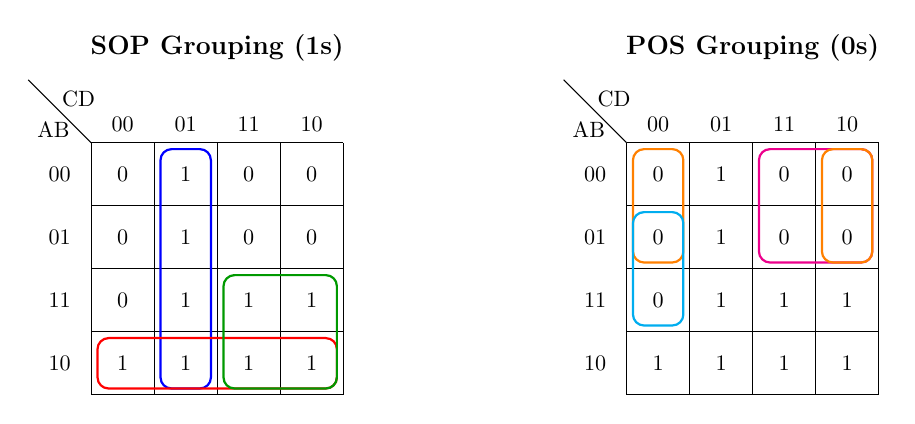
\begin{tikzpicture}[scale=0.8, every node/.style={transform shape}]
    % ---------------- LEFT K-MAP (SOP) ----------------
    \begin{scope}[xshift=0cm]
        \node at (2, 5.5) {\large \textbf{SOP Grouping (1s)}};
        \draw (0,0) grid (4,4);
        \draw (0,4) -- (-1,5);
        \node at (-0.6,4.2) {AB};
        \node at (-0.2,4.7) {CD};

        \node at (0.5,4.3) {00}; \node at (1.5,4.3) {01}; \node at (2.5,4.3) {11}; \node at (3.5,4.3) {10};
        \node at (-0.5,3.5) {00}; \node at (-0.5,2.5) {01}; \node at (-0.5,1.5) {11}; \node at (-0.5,0.5) {10};

        % Populate Cells
        \node at (0.5,3.5) {0}; \node at (1.5,3.5) {1}; \node at (2.5,3.5) {0}; \node at (3.5,3.5) {0};
        \node at (0.5,2.5) {0}; \node at (1.5,2.5) {1}; \node at (2.5,2.5) {0}; \node at (3.5,2.5) {0};
        \node at (0.5,1.5) {0}; \node at (1.5,1.5) {1}; \node at (2.5,1.5) {1}; \node at (3.5,1.5) {1};
        \node at (0.5,0.5) {1}; \node at (1.5,0.5) {1}; \node at (2.5,0.5) {1}; \node at (3.5,0.5) {1};

        % SOP Groupings
        \draw[rounded corners, blue, thick] (1.1, 0.1) rectangle (1.9, 3.9);
        \draw[rounded corners, red, thick] (0.1, 0.1) rectangle (3.9, 0.9);
        \draw[rounded corners, green!60!black, thick] (2.1, 0.1) rectangle (3.9, 1.9);
    \end{scope}

    % ---------------- RIGHT K-MAP (POS) ----------------
    \begin{scope}[xshift=8.5cm]
        \node at (2, 5.5) {\large \textbf{POS Grouping (0s)}};
        \draw (0,0) grid (4,4);
        \draw (0,4) -- (-1,5);
        \node at (-0.6,4.2) {AB};
        \node at (-0.2,4.7) {CD};

        \node at (0.5,4.3) {00}; \node at (1.5,4.3) {01}; \node at (2.5,4.3) {11}; \node at (3.5,4.3) {10};
        \node at (-0.5,3.5) {00}; \node at (-0.5,2.5) {01}; \node at (-0.5,1.5) {11}; \node at (-0.5,0.5) {10};

        % Populate Cells
        \node at (0.5,3.5) {0}; \node at (1.5,3.5) {1}; \node at (2.5,3.5) {0}; \node at (3.5,3.5) {0};
        \node at (0.5,2.5) {0}; \node at (1.5,2.5) {1}; \node at (2.5,2.5) {0}; \node at (3.5,2.5) {0};
        \node at (0.5,1.5) {0}; \node at (1.5,1.5) {1}; \node at (2.5,1.5) {1}; \node at (3.5,1.5) {1};
        \node at (0.5,0.5) {1}; \node at (1.5,0.5) {1}; \node at (2.5,0.5) {1}; \node at (3.5,0.5) {1};

        % POS Groupings
        \draw[rounded corners, magenta, thick] (2.1, 2.1) rectangle (3.9, 3.9);
        \draw[rounded corners, orange, thick] (0.1, 2.1) rectangle (0.9, 3.9);
        \draw[rounded corners, orange, thick] (3.1, 2.1) rectangle (3.9, 3.9);
        \draw[rounded corners, cyan, thick] (0.1, 1.1) rectangle (0.9, 2.9);
    \end{scope}
\end{tikzpicture}
\end{center}

\vspace{0.2cm}
\begin{itemize}
    \item \textbf{SOP Extraction:} By grouping the $1$s, we extract the minterms.
    \begin{itemize}
        \item \textcolor{blue}{\textbf{Blue Column (01):}} Constant $C=0, D=1 \implies C'D$
        \item \textcolor{red}{\textbf{Red Row (10):}} Constant $A=1, B=0 \implies AB'$
        \item \textcolor{green!60!black}{\textbf{Green 2x2 Square:}} Constant $A=1, C=1 \implies AC$
    \end{itemize}
    Summing these groups confirms $\mathbf{F_{SOP} = C'D + AB' + AC}$.

    \item \textbf{POS Extraction:} By grouping the $0$s, we extract the maxterms. Recall that for maxterms, logic is inverted ($0 \to$ uncomplemented, $1 \to$ complemented).
    \begin{itemize}
        \item \textcolor{magenta}{\textbf{Magenta 2x2 Square:}} Constant $A=0, C=1 \implies (A + C')$
        \item \textcolor{orange}{\textbf{Orange Edges (Top Corners):}} Constant $A=0, D=0 \implies (A + D)$
        \item \textcolor{cyan}{\textbf{Cyan 1x2 Rectangle:}} Constant $B=1, C=0, D=0 \implies (B' + C + D)$
    \end{itemize}
    Multiplying these groups confirms $\mathbf{F_{POS} = (A + C')(A + D)(B' + C + D)}$.
\end{itemize}

\end{tcolorbox}

\item Simplify the following expression to POS and SOP: $BCD' + ABC' + ACD$.
\mk{8} \yr{CSE 205 | L-2/T-1 | 2017--18}

\begin{tcolorbox}[enhanced,breakable,ansbox,colback=cA!4,colframe=cA,boxrule=0.8pt,arc=5pt,title={\textbf{Answer}},fonttitle=\bfseries\color{white},colbacktitle=cA]

\textbf{Simplification of the Boolean Expression}

Given the Boolean function:
\[ F = BCD' + ABC' + ACD \]
We will simplify this expression into its minimum Sum of Products (SOP) and Product of Sums (POS) forms algebraically, and then verify our results using Karnaugh Maps.

\vspace{0.3cm}
\textbf{Step 1: Algebraic Simplification to Sum of Products (SOP)}

We can simplify the given expression step-by-step using fundamental Boolean algebra laws, specifically relying on the \textbf{Consensus Theorem} ($XY + X'Z + YZ = XY + X'Z$). 

Observe the terms $BCD'$ and $ACD$. The variable $D$ is uncomplemented in the latter and complemented in the former. The consensus of these two terms is $(BC)(AC) = ABC$. By the Consensus Theorem, we can add this redundant term without changing the function's value:
\begin{align*}
F &= BCD' + ABC' + ACD \\
F &= BCD' + ABC' + ACD + ABC \quad &&\text{(Adding consensus of } BCD' \text{ and } ACD \text{)} \\
F &= BCD' + ACD + ABC' + ABC \quad &&\text{(Rearranging terms)} \\
F &= BCD' + ACD + AB(C' + C) \quad &&\text{(Factoring } AB \text{)} \\
F &= BCD' + ACD + AB(1) \quad &&\text{(Complement Law: } C' + C = 1 \text{)} \\
F &= BCD' + ACD + AB \quad &&\text{(Identity Law)}
\end{align*}
Rearranging to a standard order, the simplified \textbf{SOP} expression is:
\[ \mathbf{F_{SOP} = AB + ACD + BCD'} \]

\vspace{0.3cm}
\textbf{Step 2: Algebraic Simplification to Product of Sums (POS)}

We derive the POS form directly from our minimal SOP expression using the Distributive Law ($X + YZ = (X + Y)(X + Z)$) and the Consensus Theorem.
\begin{align*}
F &= AB + ACD + BCD' \\
F &= AB + C(AD + BD') \quad &&\text{(Factoring } C \text{ from the last two terms)} \\
F &= (AB + C)(AB + AD + BD') \quad &&\text{(Distributive Law)}
\end{align*}
Now, we simplify both factors:
\begin{enumerate}
    \item \textbf{First factor:} By the Distributive Law, $(AB + C) = (A + C)(B + C)$.
    \item \textbf{Second factor:} Notice that $AB$ is the consensus of $AD$ and $BD'$. Therefore, $AD + BD' + AB = AD + BD'$. We can use this property to eliminate $AB$:
    \[ AB + AD + BD' = AD + BD' \]
    Furthermore, we can factor $AD + BD'$ by recognizing it is the expanded form of $(A + D')(B + D)$:
    \[ (A + D')(B + D) = AB + AD + BD' + DD' = AB + AD + BD' = AD + BD' \]
\end{enumerate}
Substituting these simplified factors back into our expression for $F$:
\begin{align*}
F &= (A + C)(B + C) \cdot (A + D')(B + D)
\end{align*}
Thus, the simplified \textbf{POS} expression is:
\[ \mathbf{F_{POS} = (A + C)(B + C)(B + D)(A + D')} \]

\vspace{0.3cm}
\textbf{Step 3: Karnaugh Map Verification}

To rigorously verify our algebraic minimizations, we plot the function on a 4-variable K-map. We derive SOP by grouping the $1$s and POS by grouping the $0$s.

\vspace{0.4cm}
\begin{center}
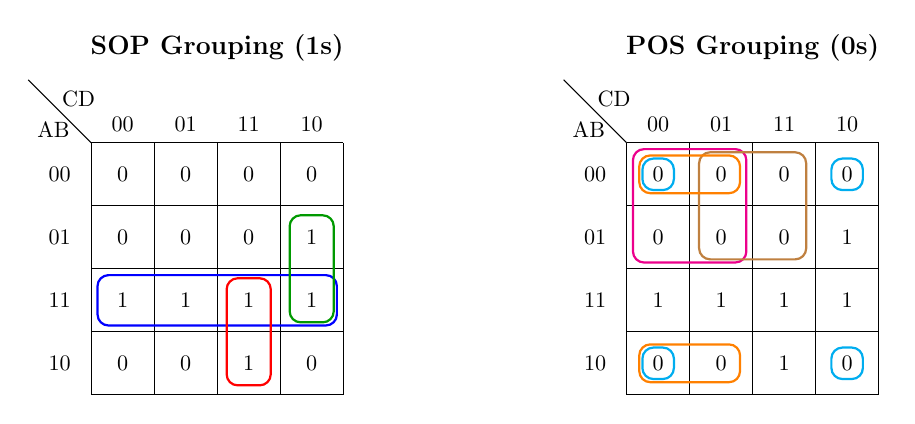
\begin{tikzpicture}[scale=0.8, every node/.style={transform shape}]
    % ---------------- LEFT K-MAP (SOP) ----------------
    \begin{scope}[xshift=0cm]
        \node at (2, 5.5) {\large \textbf{SOP Grouping (1s)}};
        \draw (0,0) grid (4,4);
        \draw (0,4) -- (-1,5);
        \node at (-0.6,4.2) {AB};
        \node at (-0.2,4.7) {CD};

        \node at (0.5,4.3) {00}; \node at (1.5,4.3) {01}; \node at (2.5,4.3) {11}; \node at (3.5,4.3) {10};
        \node at (-0.5,3.5) {00}; \node at (-0.5,2.5) {01}; \node at (-0.5,1.5) {11}; \node at (-0.5,0.5) {10};

        % Populate Cells
        \node at (0.5,3.5) {0}; \node at (1.5,3.5) {0}; \node at (2.5,3.5) {0}; \node at (3.5,3.5) {0};
        \node at (0.5,2.5) {0}; \node at (1.5,2.5) {0}; \node at (2.5,2.5) {0}; \node at (3.5,2.5) {1};
        \node at (0.5,1.5) {1}; \node at (1.5,1.5) {1}; \node at (2.5,1.5) {1}; \node at (3.5,1.5) {1};
        \node at (0.5,0.5) {0}; \node at (1.5,0.5) {0}; \node at (2.5,0.5) {1}; \node at (3.5,0.5) {0};

        % SOP Groupings
        \draw[rounded corners, blue, thick] (0.1, 1.1) rectangle (3.9, 1.9); % AB
        \draw[rounded corners, red, thick] (2.15, 0.15) rectangle (2.85, 1.85); % ACD
        \draw[rounded corners, green!60!black, thick] (3.15, 1.15) rectangle (3.85, 2.85); % BCD'
    \end{scope}

    % ---------------- RIGHT K-MAP (POS) ----------------
    \begin{scope}[xshift=8.5cm]
        \node at (2, 5.5) {\large \textbf{POS Grouping (0s)}};
        \draw (0,0) grid (4,4);
        \draw (0,4) -- (-1,5);
        \node at (-0.6,4.2) {AB};
        \node at (-0.2,4.7) {CD};

        \node at (0.5,4.3) {00}; \node at (1.5,4.3) {01}; \node at (2.5,4.3) {11}; \node at (3.5,4.3) {10};
        \node at (-0.5,3.5) {00}; \node at (-0.5,2.5) {01}; \node at (-0.5,1.5) {11}; \node at (-0.5,0.5) {10};

        % Populate Cells (Same grid)
        \node at (0.5,3.5) {0}; \node at (1.5,3.5) {0}; \node at (2.5,3.5) {0}; \node at (3.5,3.5) {0};
        \node at (0.5,2.5) {0}; \node at (1.5,2.5) {0}; \node at (2.5,2.5) {0}; \node at (3.5,2.5) {1};
        \node at (0.5,1.5) {1}; \node at (1.5,1.5) {1}; \node at (2.5,1.5) {1}; \node at (3.5,1.5) {1};
        \node at (0.5,0.5) {0}; \node at (1.5,0.5) {0}; \node at (2.5,0.5) {1}; \node at (3.5,0.5) {0};

        % POS Groupings
        \draw[rounded corners, magenta, thick] (0.1, 2.1) rectangle (1.9, 3.9); % (A+C)
        \draw[rounded corners, brown, thick] (1.15, 2.15) rectangle (2.85, 3.85); % (A+D')
        
        \draw[rounded corners, orange, thick] (0.2, 3.2) rectangle (1.8, 3.8); % (B+C) top
        \draw[rounded corners, orange, thick] (0.2, 0.2) rectangle (1.8, 0.8); % (B+C) bot
        
        \draw[rounded corners, cyan, thick] (0.25, 3.25) rectangle (0.75, 3.75); % (B+D) TL
        \draw[rounded corners, cyan, thick] (3.25, 3.25) rectangle (3.75, 3.75); % (B+D) TR
        \draw[rounded corners, cyan, thick] (0.25, 0.25) rectangle (0.75, 0.75); % (B+D) BL
        \draw[rounded corners, cyan, thick] (3.25, 0.25) rectangle (3.75, 0.75); % (B+D) BR
    \end{scope}
\end{tikzpicture}
\end{center}

\vspace{0.2cm}
\begin{itemize}
    \item \textbf{SOP Extraction (1s):} 
    \begin{itemize}
        \item \textcolor{blue}{\textbf{Blue Row:}} Constant $A=1, B=1 \implies AB$
        \item \textcolor{red}{\textbf{Red Column Pair:}} Constant $A=1, C=1, D=1 \implies ACD$
        \item \textcolor{green!60!black}{\textbf{Green Column Pair:}} Constant $B=1, C=1, D=0 \implies BCD'$
    \end{itemize}
    This confirms $\mathbf{F_{SOP} = AB + ACD + BCD'}$.

    \item \textbf{POS Extraction (0s):} (Note: $0 \to$ uncomplemented, $1 \to$ complemented)
    \begin{itemize}
        \item \textcolor{magenta}{\textbf{Magenta 2x2:}} Constant $A=0, C=0 \implies (A + C)$
        \item \textcolor{brown}{\textbf{Brown 2x2:}} Constant $A=0, D=1 \implies (A + D')$
        \item \textcolor{orange}{\textbf{Orange Split 2x2:}} Constant $B=0, C=0 \implies (B + C)$
        \item \textcolor{cyan}{\textbf{Cyan Four Corners:}} Constant $B=0, D=0 \implies (B + D)$
    \end{itemize}
    This confirms $\mathbf{F_{POS} = (A + C)(B + C)(B + D)(A + D')}$.
\end{itemize}

\end{tcolorbox}

\item Prove the following Boolean algebra theorem:
\[ (x + y)(x' + z)(y + z) = (x + y)(x' + z) \]
\mk{10} \yr{CSE 205 | L-2/T-1 | 2015--16}

\begin{tcolorbox}[enhanced,breakable,ansbox,colback=cA!4,colframe=cA,boxrule=0.8pt,arc=5pt,title={\textbf{Answer}},fonttitle=\bfseries\color{white},colbacktitle=cA]

\textbf{Proof of the Boolean Algebra Theorem (Consensus Theorem in POS Form)}

The given theorem is the Product of Sums (POS) form of the \textbf{Consensus Theorem}. We can prove this theorem using two rigorous methods: Algebraic Manipulation and Truth Table Verification.

\vspace{0.4cm}
\textbf{Method 1: Algebraic Proof}

We start with the Left-Hand Side (LHS) of the equation and apply standard Boolean algebra postulates and theorems to reduce it to the Right-Hand Side (RHS).

\begin{align*}
\text{LHS} &= (x + y)(x' + z)(y + z) \\
&= (x + y)(x' + z)(y + z + 0) && \text{(Identity Law: } A + 0 = A \text{)} \\
&= (x + y)(x' + z)(y + z + xx') && \text{(Complement Law: } xx' = 0 \text{)} \\
&= (x + y)(x' + z)(x + y + z)(x' + y + z) && \text{(Distributive Law: } A + BC = (A+B)(A+C) \text{)} \\
\end{align*}

Now, we rearrange the terms using the Commutative Law to group related sums together:
\begin{align*}
\text{LHS} &= \big[ (x + y)(x + y + z) \big] \cdot \big[ (x' + z)(x' + z + y) \big] && \text{(Commutative Law)} 
\end{align*}

Next, we apply the \textbf{Absorption Law}, which states that $A(A + B) = A$. 
\begin{itemize}
    \item For the first group, let $A = (x + y)$ and $B = z$. Thus, $(x + y)(x + y + z) = (x + y)$.
    \item For the second group, let $A = (x' + z)$ and $B = y$. Thus, $(x' + z)(x' + z + y) = (x' + z)$.
\end{itemize}

Substituting these absorbed expressions back into our main equation gives:
\begin{align*}
\text{LHS} &= (x + y)(x' + z) \\
&= \text{RHS}
\end{align*}
\textbf{Thus, the theorem is algebraically proven.}

\vspace{0.6cm}
\textbf{Method 2: Verification via Truth Table}

To ensure complete verification of the circuit behavior, we can exhaustively test all possible combinations of the variables $x, y,$ and $z$. 

\begin{center}
\renewcommand{\arraystretch}{1.3}
\begin{tabular}{|c|c|c||c|c|c|c||c|c|}
\hline
\textbf{$x$} & \textbf{$y$} & \textbf{$z$} & \textbf{$x'$} & \textbf{Term 1:} $(x+y)$ & \textbf{Term 2:} $(x'+z)$ & \textbf{Term 3:} $(y+z)$ & \textbf{LHS:} T1 $\cdot$ T2 $\cdot$ T3 & \textbf{RHS:} T1 $\cdot$ T2 \\
\hline
$0$ & $0$ & $0$ & $1$ & $0$ & $1$ & $0$ & \textbf{0} & \textbf{0} \\
\hline
$0$ & $0$ & $1$ & $1$ & $0$ & $1$ & $1$ & \textbf{0} & \textbf{0} \\
\hline
$0$ & $1$ & $0$ & $1$ & $1$ & $1$ & $1$ & \textbf{1} & \textbf{1} \\
\hline
$0$ & $1$ & $1$ & $1$ & $1$ & $1$ & $1$ & \textbf{1} & \textbf{1} \\
\hline
$1$ & $0$ & $0$ & $0$ & $1$ & $0$ & $0$ & \textbf{0} & \textbf{0} \\
\hline
$1$ & $0$ & $1$ & $0$ & $1$ & $1$ & $1$ & \textbf{1} & \textbf{1} \\
\hline
$1$ & $1$ & $0$ & $0$ & $1$ & $0$ & $1$ & \textbf{0} & \textbf{0} \\
\hline
$1$ & $1$ & $1$ & $0$ & $1$ & $1$ & $1$ & \textbf{1} & \textbf{1} \\
\hline
\end{tabular}
\end{center}

\vspace{0.2cm}
By comparing the last two columns of the truth table, we observe that the output values for the LHS $(x + y)(x' + z)(y + z)$ and the RHS $(x + y)(x' + z)$ are identical for every possible input combination of $x, y,$ and $z$. 

\textbf{Conclusion:} Both the rigorous algebraic derivation and the exhaustive truth table prove that the expression $(x + y)(x' + z)(y + z)$ accurately simplifies to $(x + y)(x' + z)$.
\end{tcolorbox}

\item How many distinct Boolean functions are there of $n$ Boolean variables?
\mk{5} \yr{CSE 205 | L-2/T-1 | 2015--16}

\begin{tcolorbox}[enhanced,breakable,ansbox,colback=cA!4,colframe=cA,boxrule=0.8pt,arc=5pt,title={\textbf{Answer}},fonttitle=\bfseries\color{white},colbacktitle=cA]

\textbf{Total Number of Distinct Boolean Functions}

For $n$ Boolean variables, the total number of distinct Boolean functions is given by the formula:
\[ \mathbf{2^{2^n}} \]

\vspace{0.3cm}
\textbf{Step-by-Step Derivation:}

To understand how this formula is derived mathematically, we can analyze the structure of a standard logic truth table.

\begin{enumerate}
    \item \textbf{Determine the number of input combinations:} 
    A Boolean function of $n$ variables (e.g., $x_1, x_2, \dots, x_n$) operates on inputs that can each take on exactly two possible values in binary logic: $0$ or $1$. Therefore, the total number of unique input combinations (which corresponds to the number of rows in the truth table) is:
    \[ \text{Number of Rows} = 2 \times 2 \times \dots \times 2 \text{ ($n$ times)} = 2^n \]
    
    \item \textbf{Determine the number of output assignments:}
    A specific Boolean function is uniquely defined by the output value it maps to each of these $2^n$ input combinations. For every single row in the truth table, the function's output can be either a $0$ or a $1$. This gives exactly $2$ independent choices per row.
    
    \item \textbf{Calculate the total possible functions:}
    Since there are $2$ choices for the output of the first row, $2$ choices for the second row, and so on, spanning across all $2^n$ rows, the fundamental counting principle dictates that we multiply the number of choices together:
    \[ \text{Total Functions} = \underbrace{2 \times 2 \times 2 \times \dots \times 2}_{2^n \text{ times}} = 2^{(2^n)} \]
\end{enumerate}

\vspace{0.3cm}
\textbf{Illustrative Examples:}

To verify this intuitively, we can evaluate the formula for small values of $n$.

\begin{itemize}
    \item \textbf{Case for $n = 1$ (One variable, e.g., $A$):}
    \begin{itemize}
        \item Number of input rows: $2^1 = 2$ rows (Inputs $A=0$ and $A=1$).
        \item Number of possible functions: $2^{2^1} = 2^2 = \mathbf{4}$ distinct functions.
        \item These 4 functions are: $F = 0$ (Constant 0), $F = 1$ (Constant 1), $F = A$ (Buffer/Identity), and $F = A'$ (NOT/Inverter).
    \end{itemize}
    
    \vspace{0.2cm}
    \item \textbf{Case for $n = 2$ (Two variables, e.g., $A, B$):}
    \begin{itemize}
        \item Number of input rows: $2^2 = 4$ rows (Inputs $00, 01, 10, 11$).
        \item Number of possible functions: $2^{2^2} = 2^4 = \mathbf{16}$ distinct functions.
        \item These 16 functions represent all possible 2-input logic mappings, including standard logic gates such as AND, OR, NAND, NOR, XOR, XNOR, Implications, Constants, and single-variable passes/inversions.
    \end{itemize}
    
    \vspace{0.2cm}
    \item \textbf{Case for $n = 3$ (Three variables):}
    \begin{itemize}
        \item Number of input rows: $2^3 = 8$ rows.
        \item Number of possible functions: $2^{2^3} = 2^8 = \mathbf{256}$ distinct Boolean functions.
    \end{itemize}
\end{itemize}

\vspace{0.3cm}
\textbf{Summary Table of Combinatorial Growth:}

The number of functions exhibits double exponential growth, as shown below:

\begin{center}
\renewcommand{\arraystretch}{1.4}
\begin{tabular}{|c|c|c|}
\hline
\textbf{Number of Variables ($n$)} & \textbf{Truth Table Rows ($2^n$)} & \textbf{Distinct Functions ($2^{2^n}$)} \\
\hline
$1$ & $2$ & $4$ \\
\hline
$2$ & $4$ & $16$ \\
\hline
$3$ & $8$ & $256$ \\
\hline
$4$ & $16$ & $65,536$ \\
\hline
$5$ & $32$ & $4,294,967,296$ \\
\hline
\end{tabular}
\end{center}

\end{tcolorbox}

\item Simplify the Boolean function using algebraic manipulation:
\[ f = A'BC + AB'C + ABC' + ABC \]
\mk{10} \yr{CSE 205 | L-2/T-1 | 2015--16}

\begin{tcolorbox}[enhanced,breakable,ansbox,colback=cA!4,colframe=cA,boxrule=0.8pt,arc=5pt,title={\textbf{Answer}},fonttitle=\bfseries\color{white},colbacktitle=cA]

\textbf{Algebraic Simplification of the Boolean Function}

The given Boolean function is:
\[ f = A'BC + AB'C + ABC' + ABC \]

This function represents the Sum of Products (SOP) form of the logical Majority Function (or the Carry-Out of a Full Adder). We can simplify this expression step-by-step using standard Boolean algebraic laws.

\vspace{0.3cm}
\textbf{Step-by-Step Derivation:}

\begin{align*}
f &= A'BC + AB'C + ABC' + ABC \\
\intertext{According to the \textbf{Idempotent Law} ($X + X = X$), we can duplicate the term $ABC$ multiple times without changing the value of the function. We will add two extra copies of $ABC$ to group with the other three terms:}
f &= A'BC + AB'C + ABC' + (ABC + ABC + ABC) \\
\intertext{Now, we use the \textbf{Commutative Law} to rearrange the terms, pairing one $ABC$ with each of the other terms:}
f &= (A'BC + ABC) + (AB'C + ABC) + (ABC' + ABC) \\
\intertext{Next, we apply the \textbf{Distributive Law} ($XY + XZ = X(Y + Z)$) to factor out the common variables in each grouped pair:}
f &= BC(A' + A) + AC(B' + B) + AB(C' + C) \\
\intertext{According to the \textbf{Complement Law}, the OR sum of a variable and its complement is always 1 ($X + X' = 1$):}
f &= BC(1) + AC(1) + AB(1) \\
\intertext{Finally, applying the \textbf{Identity Law} ($X \cdot 1 = X$), we remove the 1s to obtain the simplified minimal Sum of Products expression:}
f &= BC + AC + AB
\end{align*}

Rearranging the terms alphabetically for standard presentation, we get the final simplified expression:
\[ \mathbf{f = AB + BC + AC} \]

\vspace{0.4cm}
\textbf{Verification using Karnaugh Map (Visualization)}

To visually verify our algebraic simplification, we can map the original standard SOP function onto a 3-variable Karnaugh Map. 

The original function $f = A'BC + AB'C + ABC' + ABC$ corresponds to minterms $m_3, m_5, m_6,$ and $m_7$.

\begin{center}
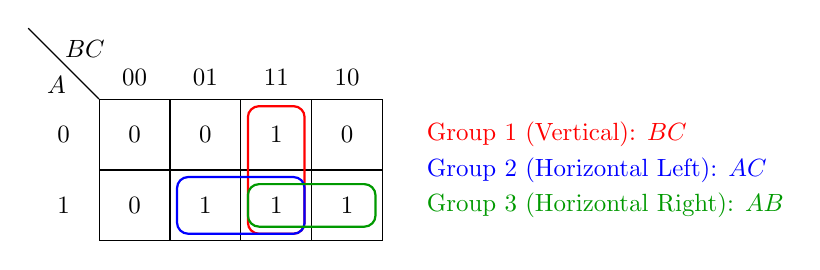
\begin{tikzpicture}[scale=0.9, every node/.style={transform shape}]
    % K-map Grid
    \draw (0,0) grid (4,2);
    \draw (0,2) -- (-1,3);
    \node at (-0.6,2.2) {$A$};
    \node at (-0.2,2.7) {$BC$};

    % Column labels (BC)
    \node at (0.5,2.3) {00}; \node at (1.5,2.3) {01}; \node at (2.5,2.3) {11}; \node at (3.5,2.3) {10};
    % Row labels (A)
    \node at (-0.5,1.5) {0}; \node at (-0.5,0.5) {1};

    % Minterm placements
    % A=0
    \node at (0.5,1.5) {0}; % 000
    \node at (1.5,1.5) {0}; % 001
    \node at (2.5,1.5) {1}; % 011 (m3) -> A'BC
    \node at (3.5,1.5) {0}; % 010
    
    % A=1
    \node at (0.5,0.5) {0}; % 100
    \node at (1.5,0.5) {1}; % 101 (m5) -> AB'C
    \node at (2.5,0.5) {1}; % 111 (m7) -> ABC
    \node at (3.5,0.5) {1}; % 110 (m6) -> ABC'

    % Groupings
    % Group 1: BC (m3, m7)
    \draw[rounded corners, red, thick] (2.1, 0.1) rectangle (2.9, 1.9);
    % Group 2: AC (m5, m7)
    \draw[rounded corners, blue, thick] (1.1, 0.1) rectangle (2.9, 0.9);
    % Group 3: AB (m7, m6)
    \draw[rounded corners, green!60!black, thick] (2.1, 0.2) rectangle (3.9, 0.8);
    
    % Legend
    \node[red, right] at (4.5, 1.5) {Group 1 (Vertical): $BC$};
    \node[blue, right] at (4.5, 1.0) {Group 2 (Horizontal Left): $AC$};
    \node[green!60!black, right] at (4.5, 0.5) {Group 3 (Horizontal Right): $AB$};
\end{tikzpicture}
\end{center}

\vspace{0.2cm}
From the K-map, we form three overlapping groups of two adjacent 1s:
\begin{itemize}
    \item \textcolor{red}{\textbf{Red Group}} covers $m_3$ and $m_7$, where $B$ and $C$ remain constant ($11$). This gives the term \textbf{$BC$}.
    \item \textcolor{blue}{\textbf{Blue Group}} covers $m_5$ and $m_7$, where $A$ and $C$ remain constant ($1$ and $1$). This gives the term \textbf{$AC$}.
    \item \textcolor{green!60!black}{\textbf{Green Group}} covers $m_6$ and $m_7$, where $A$ and $B$ remain constant ($11$). This gives the term \textbf{$AB$}.
\end{itemize}

Combining these groupings yields $f = AB + BC + AC$, which perfectly matches our algebraic derivation.

\end{tcolorbox}

\item Simplify the following Boolean function using algebraic manipulation:
\[ (A + BC)' + AB' \]
\mk{7} \yr{CSE 205 | L-2/T-1 | 2015--16}

\begin{tcolorbox}[enhanced,breakable,ansbox,colback=cA!4,colframe=cA,boxrule=0.8pt,arc=5pt,title={\textbf{Answer}},fonttitle=\bfseries\color{white},colbacktitle=cA]

\textbf{Algebraic Simplification of the Boolean Function}

The given Boolean expression is:
\[ f = (A + BC)' + AB' \]

We can simplify this function step-by-step using standard Boolean algebraic theorems and postulates.

\vspace{0.3cm}
\textbf{Step-by-Step Derivation:}

\begin{align*}
f &= (A + BC)' + AB' \\
\intertext{\textbf{Step 1:} Apply \textbf{De Morgan's Law} $(X + Y)' = X'Y'$ to the first term, treating $A$ as $X$ and $BC$ as $Y$.}
f &= A'(BC)' + AB' 
\intertext{\textbf{Step 2:} Apply \textbf{De Morgan's Law} $(XY)' = X' + Y'$ to the term $(BC)'$.}
f &= A'(B' + C') + AB' 
\intertext{\textbf{Step 3:} Apply the \textbf{Distributive Law} $X(Y + Z) = XY + XZ$ to expand the first part of the expression.}
f &= A'B' + A'C' + AB' 
\intertext{\textbf{Step 4:} Rearrange the terms using the \textbf{Commutative Law} ($X + Y = Y + X$) to place terms containing $B'$ adjacent to each other.}
f &= A'B' + AB' + A'C' 
\intertext{\textbf{Step 5:} Apply the \textbf{Distributive Law} in reverse to factor out the common literal $B'$ from the first two terms.}
f &= B'(A' + A) + A'C' 
\intertext{\textbf{Step 6:} Apply the \textbf{Complement Law}, which states that the logical OR of a variable and its complement is always true ($X' + X = 1$).}
f &= B'(1) + A'C' 
\intertext{\textbf{Step 7:} Finally, apply the \textbf{Identity Law} ($X \cdot 1 = X$) to eliminate the 1.}
f &= B' + A'C'
\end{align*}

The final simplified Boolean expression is:
\[ \mathbf{f = B' + A'C'} \]

\vspace{0.4cm}
\textbf{Verification using Truth Table}

To ensure the accuracy of our algebraic simplification, we can construct a truth table comparing the original function to our simplified result across all possible input combinations for $A$, $B$, and $C$.

\begin{center}
\renewcommand{\arraystretch}{1.3}
\begin{tabular}{|c|c|c||c|c|c|c|c||c||c|}
\hline
\textbf{$A$} & \textbf{$B$} & \textbf{$C$} & \textbf{$A'$} & \textbf{$B'$} & \textbf{$C'$} & \textbf{Term 1:} $(A+BC)'$ & \textbf{Term 2:} $AB'$ & \textbf{Original:} $(A+BC)'+AB'$ & \textbf{Simplified:} $B'+A'C'$ \\
\hline
$0$ & $0$ & $0$ & $1$ & $1$ & $1$ & $(0+0)' = 1$ & $0 \cdot 1 = 0$ & $1 + 0 = \textbf{1}$ & $1 + (1\cdot 1) = \textbf{1}$ \\
\hline
$0$ & $0$ & $1$ & $1$ & $1$ & $0$ & $(0+0)' = 1$ & $0 \cdot 1 = 0$ & $1 + 0 = \textbf{1}$ & $1 + (1\cdot 0) = \textbf{1}$ \\
\hline
$0$ & $1$ & $0$ & $1$ & $0$ & $1$ & $(0+0)' = 1$ & $0 \cdot 0 = 0$ & $1 + 0 = \textbf{1}$ & $0 + (1\cdot 1) = \textbf{1}$ \\
\hline
$0$ & $1$ & $1$ & $1$ & $0$ & $0$ & $(0+1)' = 0$ & $0 \cdot 0 = 0$ & $0 + 0 = \textbf{0}$ & $0 + (1\cdot 0) = \textbf{0}$ \\
\hline
$1$ & $0$ & $0$ & $0$ & $1$ & $1$ & $(1+0)' = 0$ & $1 \cdot 1 = 1$ & $0 + 1 = \textbf{1}$ & $1 + (0\cdot 1) = \textbf{1}$ \\
\hline
$1$ & $0$ & $1$ & $0$ & $1$ & $0$ & $(1+0)' = 0$ & $1 \cdot 1 = 1$ & $0 + 1 = \textbf{1}$ & $1 + (0\cdot 0) = \textbf{1}$ \\
\hline
$1$ & $1$ & $0$ & $0$ & $0$ & $1$ & $(1+0)' = 0$ & $1 \cdot 0 = 0$ & $0 + 0 = \textbf{0}$ & $0 + (0\cdot 1) = \textbf{0}$ \\
\hline
$1$ & $1$ & $1$ & $0$ & $0$ & $0$ & $(1+1)' = 0$ & $1 \cdot 0 = 0$ & $0 + 0 = \textbf{0}$ & $0 + (0\cdot 0) = \textbf{0}$ \\
\hline
\end{tabular}
\end{center}

\vspace{0.2cm}
\textbf{Conclusion:} 
By observing the last two columns of the truth table, we see that the output vectors for the original function $(A+BC)'+AB'$ and the simplified expression $B'+A'C'$ match perfectly for all $2^3 = 8$ possible input combinations. This conclusively proves that our algebraic simplification is correct.

\end{tcolorbox}

\item State and prove the consensus theorem using Boolean algebra.
\mk{8} \yr{CSE 205 | L-2/T-1 | 2014--15}

\begin{tcolorbox}[enhanced,breakable,ansbox,colback=cA!4,colframe=cA,boxrule=0.8pt,arc=5pt,title={\textbf{Answer}},fonttitle=\bfseries\color{white},colbacktitle=cA]

\textbf{Statement of the Consensus Theorem}

The Consensus Theorem is a powerful rule in Boolean algebra used to minimize logic expressions by eliminating redundant terms. It states that if a Boolean expression contains two terms where one variable appears uncomplemented in one term and complemented in the other, and a third term contains the remaining variables from the first two terms, this third term is redundant and can be omitted. The redundant third term is known as the \textbf{consensus term}.

The theorem exists in two dual forms:
\begin{itemize}
    \item \textbf{Sum of Products (SOP) Form:} \[ XY + X'Z + YZ = XY + X'Z \]
    \item \textbf{Product of Sums (POS) Form:} \[ (X + Y)(X' + Z)(Y + Z) = (X + Y)(X' + Z) \]
\end{itemize}

\vspace{0.4cm}
\textbf{Proof of the Sum of Products (SOP) Form}

We will prove the SOP form using standard Boolean algebraic postulates and theorems, starting with the Left-Hand Side (LHS) and simplifying it to match the Right-Hand Side (RHS).

\begin{align*}
\text{LHS} &= XY + X'Z + YZ \\
\intertext{\textbf{Step 1:} Multiply the consensus term ($YZ$) by $1$ using the \textbf{Identity Law} ($A \cdot 1 = A$).}
&= XY + X'Z + YZ \cdot 1 \\
\intertext{\textbf{Step 2:} Substitute $1$ with $(X + X')$ using the \textbf{Complement Law} ($A + A' = 1$).}
&= XY + X'Z + YZ(X + X') \\
\intertext{\textbf{Step 3:} Expand the expression using the \textbf{Distributive Law} ($A(B + C) = AB + AC$).}
&= XY + X'Z + XYZ + X'YZ \\
\intertext{\textbf{Step 4:} Rearrange the terms using the \textbf{Commutative Law} to group related terms together.}
&= XY + XYZ + X'Z + X'YZ \\
\intertext{\textbf{Step 5:} Factor out common variables using the \textbf{Distributive Law} in reverse.}
&= XY(1 + Z) + X'Z(1 + Y) \\
\intertext{\textbf{Step 6:} Apply the \textbf{Annulment Law} (also known as the Null Law), which states that $1 + A = 1$.}
&= XY(1) + X'Z(1) \\
\intertext{\textbf{Step 7:} Finally, apply the \textbf{Identity Law} ($A \cdot 1 = A$) to yield the RHS.}
&= XY + X'Z \\
&= \text{RHS}
\end{align*}
\textbf{Thus, the SOP form of the Consensus Theorem is algebraically proven.}

\vspace{0.4cm}
\textbf{Proof of the Product of Sums (POS) Form}

Similarly, we can prove the POS form by direct algebraic manipulation.

\begin{align*}
\text{LHS} &= (X + Y)(X' + Z)(Y + Z) \\
\intertext{\textbf{Step 1:} Add $0$ to the consensus term $(Y + Z)$ using the \textbf{Identity Law} ($A + 0 = A$).}
&= (X + Y)(X' + Z)(Y + Z + 0) \\
\intertext{\textbf{Step 2:} Substitute $0$ with $XX'$ using the \textbf{Complement Law} ($A \cdot A' = 0$).}
&= (X + Y)(X' + Z)(Y + Z + XX') \\
\intertext{\textbf{Step 3:} Expand using the \textbf{Distributive Law} ($A + BC = (A + B)(A + C)$).}
&= (X + Y)(X' + Z)(X + Y + Z)(X' + Y + Z) \\
\intertext{\textbf{Step 4:} Rearrange terms using the \textbf{Commutative Law} to pair terms efficiently.}
&= \big[ (X + Y)(X + Y + Z) \big] \cdot \big[ (X' + Z)(X' + Z + Y) \big] \\
\intertext{\textbf{Step 5:} Apply the \textbf{Absorption Law} $A(A + B) = A$. In the first bracketed group, let $A = X+Y$ and $B=Z$. In the second group, let $A = X'+Z$ and $B=Y$.}
&= (X + Y) \cdot (X' + Z) \\
&= \text{RHS}
\end{align*}
\textbf{Thus, the POS form of the Consensus Theorem is also algebraically proven.}

\end{tcolorbox}

\item Simplify the following function using Boolean algebra:
\[ F(A, B, C) = A'BC + AB'C + ABC \]
\mk{7} \yr{CSE 205 | L-2/T-1 | 2014--15}

\begin{tcolorbox}[enhanced,breakable,ansbox,colback=cA!4,colframe=cA,boxrule=0.8pt,arc=5pt,title={\textbf{Answer}},fonttitle=\bfseries\color{white},colbacktitle=cA]

\textbf{Algebraic Simplification of the Boolean Function}

The given Boolean function is:
\[ F(A, B, C) = A'BC + AB'C + ABC \]

We can simplify this expression step-by-step using standard Boolean algebraic postulates and theorems. There are multiple valid algebraic paths to reach the minimal form; we will use the highly effective Redundancy Law (also known as the Simplification Theorem).

\vspace{0.3cm}
\textbf{Step-by-Step Derivation:}

\begin{align*}
F &= A'BC + AB'C + ABC \\
\intertext{\textbf{Step 1:} Apply the \textbf{Distributive Law} ($XY + XZ = X(Y + Z)$) to factor out the common variables $AC$ from the second and third terms.}
F &= A'BC + AC(B' + B) \\
\intertext{\textbf{Step 2:} Apply the \textbf{Complement Law}, which states that the logical OR of a variable and its complement is always 1 ($X + X' = 1$). Here, $B' + B = 1$.}
F &= A'BC + AC(1) \\
\intertext{\textbf{Step 3:} Apply the \textbf{Identity Law} ($X \cdot 1 = X$) to eliminate the 1.}
F &= A'BC + AC \\
\intertext{\textbf{Step 4:} Apply the \textbf{Distributive Law} again to factor out the common variable $C$ from both remaining terms.}
F &= C(A'B + A) \\
\intertext{\textbf{Step 5:} Apply the \textbf{Commutative Law} to rearrange the terms inside the parenthesis for clarity.}
F &= C(A + A'B) \\
\intertext{\textbf{Step 6:} Apply the \textbf{Redundancy Law} (or Rule of Simplification), which states that $X + X'Y = X + Y$. Let $X = A$ and $Y = B$.}
F &= C(A + B) \\
\intertext{\textbf{Step 7:} Finally, expand the expression using the \textbf{Distributive Law} to present the answer in standard Sum of Products (SOP) form.}
F &= AC + BC
\end{align*}

The final simplified Boolean expression is:
\[ \mathbf{F = AC + BC} \quad \text{or} \quad \mathbf{F = C(A + B)} \]

\vspace{0.4cm}
\textbf{Verification using Karnaugh Map (Visualization)}

To rigorously verify our algebraic simplification, we can map the original function onto a 3-variable Karnaugh Map. 

The original function $F = A'BC + AB'C + ABC$ corresponds to the minterms $m_3$ ($011$), $m_5$ ($101$), and $m_7$ ($111$).

\begin{center}
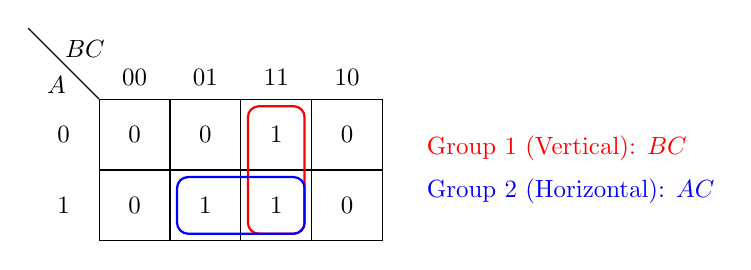
\begin{tikzpicture}[scale=0.9, every node/.style={transform shape}]
    % K-map Grid
    \draw (0,0) grid (4,2);
    \draw (0,2) -- (-1,3);
    \node at (-0.6,2.2) {$A$};
    \node at (-0.2,2.7) {$BC$};

    % Column labels (BC)
    \node at (0.5,2.3) {00}; \node at (1.5,2.3) {01}; \node at (2.5,2.3) {11}; \node at (3.5,2.3) {10};
    % Row labels (A)
    \node at (-0.5,1.5) {0}; \node at (-0.5,0.5) {1};

    % Minterm placements
    % A=0
    \node at (0.5,1.5) {0}; % 000
    \node at (1.5,1.5) {0}; % 001
    \node at (2.5,1.5) {1}; % 011 (m3) -> A'BC
    \node at (3.5,1.5) {0}; % 010
    
    % A=1
    \node at (0.5,0.5) {0}; % 100
    \node at (1.5,0.5) {1}; % 101 (m5) -> AB'C
    \node at (2.5,0.5) {1}; % 111 (m7) -> ABC
    \node at (3.5,0.5) {0}; % 110 (m6)

    % Groupings
    % Group 1: BC (m3, m7)
    \draw[rounded corners, red, thick] (2.1, 0.1) rectangle (2.9, 1.9);
    % Group 2: AC (m5, m7)
    \draw[rounded corners, blue, thick] (1.1, 0.1) rectangle (2.9, 0.9);
    
    % Legend
    \node[red, right] at (4.5, 1.3) {Group 1 (Vertical): $BC$};
    \node[blue, right] at (4.5, 0.7) {Group 2 (Horizontal): $AC$};
\end{tikzpicture}
\end{center}

\vspace{0.2cm}
By analyzing the K-map, we can form two optimal groups of adjacent 1s:
\begin{itemize}
    \item \textcolor{red}{\textbf{Red Group}} covers minterms $m_3$ and $m_7$. In this vertical group, $A$ changes from $0$ to $1$ (and is eliminated), while $B$ and $C$ remain constant at $11$. This yields the term \textbf{$BC$}.
    \item \textcolor{blue}{\textbf{Blue Group}} covers minterms $m_5$ and $m_7$. In this horizontal group, $B$ changes from $0$ to $1$ (and is eliminated), while $A$ and $C$ remain constant at $1$ and $1$. This yields the term \textbf{$AC$}.
\end{itemize}

Combining the terms derived from the logical groupings yields $F = AC + BC$. This visual minimization perfectly corroborates our step-by-step algebraic simplification.

\end{tcolorbox}

\item Simplify the following Boolean expressions to a minimum number of literals using Boolean algebra:
\begin{enumerate}
  \item $AB + A(CD + CD') + A'$
  \item $(A + B)'(A' + B')'$
\end{enumerate}
\mk{10} \yr{CSE 205 | L-2/T-1 | 2013--14}

\begin{tcolorbox}[enhanced,breakable,ansbox,colback=cA!4,colframe=cA,boxrule=0.8pt,arc=5pt,title={\textbf{Answer}},fonttitle=\bfseries\color{white},colbacktitle=cA]

\textbf{Boolean Algebra Simplification}

We are tasked with simplifying two Boolean expressions to their minimum number of literals. We will proceed step-by-step, clearly stating the Boolean theorems and postulates used at each stage.

\vspace{0.4cm}
\textbf{Part 1: Simplify } $\mathbf{AB + A(CD + CD') + A'}$

Let $F_1 = AB + A(CD + CD') + A'$. 

\begin{align*}
F_1 &= AB + A(CD + CD') + A' \\
\intertext{\textbf{Step 1:} Factor out the common variable $C$ from the terms inside the parentheses using the \textbf{Distributive Law} ($XY + XZ = X(Y + Z)$).}
&= AB + AC(D + D') + A' \\
\intertext{\textbf{Step 2:} Apply the \textbf{Complement Law}, which states that the logical OR of a variable and its complement is always $1$ ($X + X' = 1$). Here, $D + D' = 1$.}
&= AB + AC(1) + A' \\
\intertext{\textbf{Step 3:} Apply the \textbf{Identity Law} ($X \cdot 1 = X$) to eliminate the $1$.}
&= AB + AC + A' \\
\intertext{\textbf{Step 4:} Rearrange the terms using the \textbf{Commutative Law} ($X + Y = Y + X$) to position $A'$ next to $AB$.}
&= A' + AB + AC \\
\intertext{\textbf{Step 5:} Apply the \textbf{Distributive Law} in the form $X + YZ = (X + Y)(X + Z)$ to the first two terms: $A' + AB = (A' + A)(A' + B)$.}
&= (A' + A)(A' + B) + AC \\
\intertext{\textbf{Step 6:} Apply the \textbf{Complement Law} again ($A' + A = 1$).}
&= 1 \cdot (A' + B) + AC \\
\intertext{\textbf{Step 7:} Apply the \textbf{Identity Law} ($1 \cdot X = X$).}
&= A' + B + AC \\
\intertext{\textbf{Step 8:} Rearrange terms again using the \textbf{Commutative Law} to group $A'$ and $AC$.}
&= B + A' + AC \\
\intertext{\textbf{Step 9:} Apply the \textbf{Distributive Law} to $A' + AC$, expanding it to $(A' + A)(A' + C)$.}
&= B + (A' + A)(A' + C) \\
\intertext{\textbf{Step 10:} Use the \textbf{Complement Law} ($A' + A = 1$) and the \textbf{Identity Law} to simplify the term.}
&= B + 1 \cdot (A' + C) \\
&= B + A' + C
\end{align*}

Rearranging the variables alphabetically, the final simplified expression is:
\[ \mathbf{F_1 = A' + B + C} \]

\vspace{0.6cm}
\rule{\textwidth}{0.4pt}
\vspace{0.4cm}

\textbf{Part 2: Simplify } $\mathbf{(A + B)'(A' + B')'}$

Let $F_2 = (A + B)'(A' + B')'$.

\begin{align*}
F_2 &= (A + B)'(A' + B')' \\
\intertext{\textbf{Step 1:} Apply \textbf{De Morgan's Law} [$(X + Y)' = X'Y'$] to the first term, $(A + B)'$.}
&= (A'B') \cdot (A' + B')' \\
\intertext{\textbf{Step 2:} Apply \textbf{De Morgan's Law} again to the second term, $(A' + B')'$.}
&= (A'B') \cdot ((A')'(B')') \\
\intertext{\textbf{Step 3:} Apply the \textbf{Involution Law} (or Double Negation Law), which states $(X')' = X$, to simplify $(A')'$ to $A$ and $(B')'$ to $B$.}
&= (A'B') \cdot (AB) \\
\intertext{\textbf{Step 4:} Remove the parentheses using the \textbf{Associative Law} and rearrange the variables using the \textbf{Commutative Law} to group identical variables together.}
&= (A \cdot A') \cdot (B \cdot B') \\
\intertext{\textbf{Step 5:} Apply the \textbf{Complement Law} (AND form), which states that the logical AND of a variable and its complement is always $0$ ($X \cdot X' = 0$).}
&= 0 \cdot 0 \\
\intertext{\textbf{Step 6:} Apply the \textbf{Idempotent Law} (or Null Law) to conclude the simplification.}
&= 0
\end{align*}

The final simplified expression is:
\[ \mathbf{F_2 = 0} \]

\end{tcolorbox}

\item The Boolean expression for an X-OR gate is $AB' + A'B$. With this as a starting point, use DeMorgan's theorems and other rules or laws to find a simplified expression for an X-NOR gate.
\mk{8} \yr{CSE 205 | L-2/T-1 | 2011--12}

\begin{tcolorbox}[enhanced,breakable,ansbox,colback=cA!4,colframe=cA,boxrule=0.8pt,arc=5pt,title={\textbf{Answer}},fonttitle=\bfseries\color{white},colbacktitle=cA]

\textbf{Derivation of the X-NOR Expression}

The Exclusive-NOR (X-NOR) gate operates as the logical complement (inversion) of the Exclusive-OR (X-OR) gate. Therefore, we can derive the Boolean expression for the X-NOR gate by taking the complement of the given X-OR expression and simplifying it using Boolean algebra.

Given the X-OR expression:
\[ \text{X-OR} = AB' + A'B \]

The X-NOR expression is:
\[ \text{X-NOR} = (AB' + A'B)' \]

\vspace{0.3cm}
\textbf{Step-by-Step Algebraic Simplification:}

\begin{align*}
F_{\text{XNOR}} &= (AB' + A'B)' \\
\intertext{\textbf{Step 1:} Apply \textbf{De Morgan's Law} [$(X + Y)' = X' \cdot Y'$] to the entire expression, treating the term $AB'$ as $X$ and the term $A'B$ as $Y$.}
&= (AB')' \cdot (A'B)' \\
\intertext{\textbf{Step 2:} Apply \textbf{De Morgan's Law} [$(XY)' = X' + Y'$] individually to both grouped product terms.}
&= (A' + (B')') \cdot ((A')' + B') \\
\intertext{\textbf{Step 3:} Apply the \textbf{Involution Law} (Double Negation Law), which states that $(X')' = X$, to eliminate the double primes on variables $A$ and $B$.}
&= (A' + B) \cdot (A + B') \\
\intertext{\textbf{Step 4:} Apply the \textbf{Distributive Law} to expand the product of sums (multiplying out the terms: First, Outer, Inner, Last).}
&= A'A + A'B' + BA + BB' \\
\intertext{\textbf{Step 5:} Apply the \textbf{Commutative Law} to rearrange the term $BA$ to $AB$ for standard presentation.}
&= A'A + A'B' + AB + BB' \\
\intertext{\textbf{Step 6:} Apply the \textbf{Complement Law} (AND form), which states that a variable ANDed with its logical complement is always $0$ ($X \cdot X' = 0$). Therefore, $A'A = 0$ and $BB' = 0$.}
&= 0 + A'B' + AB + 0 \\
\intertext{\textbf{Step 7:} Apply the \textbf{Identity Law} ($X + 0 = X$) to remove the zeros from the sum.}
&= A'B' + AB \\
\intertext{\textbf{Step 8:} Apply the \textbf{Commutative Law} one final time to arrange the terms into the universally recognized standard format.}
&= AB + A'B'
\end{align*}

The simplified Boolean expression for an X-NOR gate is:
\[ \mathbf{F_{\text{XNOR}} = AB + A'B'} \]

\vspace{0.4cm}
\textbf{Verification via Truth Table}

To rigorously verify that this derived expression correctly models the X-NOR behavior (often called the Equivalence gate, outputting $1$ when inputs match), we can evaluate its truth table:

\begin{center}
\renewcommand{\arraystretch}{1.3}
\begin{tabular}{|c|c||c|c||c|c||c|}
\hline
\textbf{$A$} & \textbf{$B$} & \textbf{$A'$} & \textbf{$B'$} & \textbf{Term 1:} $AB$ & \textbf{Term 2:} $A'B'$ & \textbf{Output:} $AB + A'B'$ \\
\hline
$0$ & $0$ & $1$ & $1$ & $0$ & $1$ & \textbf{1} \\
\hline
$0$ & $1$ & $1$ & $0$ & $0$ & $0$ & \textbf{0} \\
\hline
$1$ & $0$ & $0$ & $1$ & $0$ & $0$ & \textbf{0} \\
\hline
$1$ & $1$ & $0$ & $0$ & $1$ & $0$ & \textbf{1} \\
\hline
\end{tabular}
\end{center}

\vspace{0.2cm}
\textbf{Conclusion:}
The truth table explicitly confirms that the output evaluates to $1$ only when both inputs are identical ($A=B=0$ or $A=B=1$). This fully validates that our algebraically derived expression $\mathbf{AB + A'B'}$ acts correctly as an X-NOR function.

\end{tcolorbox}

\item Give an example of the non-associativity of the 3-input NOR operator.
\mk{8} \yr{CSE 205 | L-2/T-1 | 2011--12}

\begin{tcolorbox}[enhanced,breakable,ansbox,colback=cA!4,colframe=cA,boxrule=0.8pt,arc=5pt,title={\textbf{Answer}},fonttitle=\bfseries\color{white},colbacktitle=cA]

\textbf{Non-Associativity of the 3-Input NOR Operator}

For a binary operator to be associative, the order in which grouping is applied must not affect the final result. That is, an operator $\downarrow$ (representing NOR) is associative if and only if for all possible Boolean values $A$, $B$, and $C$:
\[ (A \downarrow B) \downarrow C = A \downarrow (B \downarrow C) \]

We will demonstrate that the NOR operator is \textbf{non-associative} by using two methods: algebraic expansion and a definitive truth-table counterexample.

\vspace{0.3cm}
\textbf{1. Algebraic Demonstration}

The NOR operation between two variables is defined as the complement of their logical sum: 
\[ X \downarrow Y = (X + Y)' \]

Let us expand both sides of the associative equation using De Morgan's laws:

\begin{itemize}
    \item \textbf{Left-Hand Side (LHS):}
    \begin{align*}
    \text{LHS} &= (A \downarrow B) \downarrow C \\
    &= ((A + B)') \downarrow C \\
    &= \big((A + B)' + C\big)' \\
    \intertext{Applying De Morgan's Law $(X+Y)' = X'Y'$ and the Involution Law $(X'') = X$:}
    &= ((A + B)')' \cdot C' \\
    &= (A + B)C' \\
    &= AC' + BC'
    \end{align*}

    \item \textbf{Right-Hand Side (RHS):}
    \begin{align*}
    \text{RHS} &= A \downarrow (B \downarrow C) \\
    &= A \downarrow ((B + C)') \\
    &= \big(A + (B + C)'\big)' \\
    \intertext{Applying De Morgan's Law and the Involution Law:}
    &= A' \cdot ((B + C)')' \\
    &= A'(B + C) \\
    &= A'B + A'C
    \end{align*}
\end{itemize}

Since the expanded expressions $\mathbf{AC' + BC'}$ (LHS) and $\mathbf{A'B + A'C}$ (RHS) are distinct and not logically equivalent, the operator is non-associative.

\vspace{0.4cm}
\textbf{2. Concrete Truth Table Counterexample}

To explicitly prove non-associativity, we evaluate all $2^3 = 8$ combinations of inputs. A single mismatch between the LHS and RHS columns is sufficient to prove non-associativity.

\begin{center}
\renewcommand{\arraystretch}{1.3}
\begin{tabular}{|c|c|c||c|c||c|c||c|}
\hline
\textbf{$A$} & \textbf{$B$} & \textbf{$C$} & \textbf{$A \downarrow B$} & \textbf{$\text{LHS}: (A \downarrow B) \downarrow C$} & \textbf{$B \downarrow C$} & \textbf{$\text{RHS}: A \downarrow (B \downarrow C)$} & \textbf{Status} \\
\hline
$0$ & $0$ & $0$ & $1$ & $(1+0)' = \mathbf{0}$ & $1$ & $(0+1)' = \mathbf{0}$ & Match \\
\hline
$0$ & $0$ & $1$ & $1$ & $(1+1)' = \mathbf{0}$ & $0$ & $(0+0)' = \mathbf{1}$ & \textbf{Mismatch} \\
\hline
$0$ & $1$ & $0$ & $0$ & $(0+0)' = \mathbf{1}$ & $0$ & $(0+0)' = \mathbf{1}$ & Match \\
\hline
$0$ & $1$ & $1$ & $0$ & $(0+1)' = \mathbf{0}$ & $0$ & $(0+0)' = \mathbf{1}$ & \textbf{Mismatch} \\
\hline
$1$ & $0$ & $0$ & $0$ & $(0+0)' = \mathbf{1}$ & $1$ & $(1+1)' = \mathbf{0}$ & \textbf{Mismatch} \\
\hline
$1$ & $0$ & $1$ & $0$ & $(0+1)' = \mathbf{0}$ & $0$ & $(1+0)' = \mathbf{0}$ & Match \\
\hline
$1$ & $1$ & $0$ & $0$ & $(0+0)' = \mathbf{1}$ & $0$ & $(1+0)' = \mathbf{0}$ & \textbf{Mismatch} \\
\hline
$1$ & $1$ & $1$ & $0$ & $(0+1)' = \mathbf{0}$ & $0$ & $(1+0)' = \mathbf{0}$ & Match \\
\hline
\end{tabular}
\end{center}

\vspace{0.2cm}
As highlighted in the table, rows such as \textbf{$(A=0, B=0, C=1)$} clearly show a conflict where $\text{LHS} = 0$ while $\text{RHS} = 1$.

\vspace{0.4cm}
\textbf{3. Structural Visualization via Logic Circuits}

The structural asymmetry causing this functional difference can be easily understood by visualizing how the inputs cascade through the hardware connections in each grouping configuration.

\begin{center}
\begin{circuitikz}[scale=1, transform shape]

    % ==========================================
    % Circuit 1: ((A NOR B) NOR C)
    % ==========================================
    \node at (2, 3.5) {\textbf{Circuit 1: } $((A \downarrow B) \downarrow C)$};
    
    % NOR Gates for Circuit 1
    \node[nor port] (nor1) at (2, 2.2) {};
    \node[nor port] (nor2) at (4.5, 1.3) {};
    
    % Connections for Circuit 1
    \draw (nor1.in 1) -- ++(-1.5,0) node[left] {$A$};
    \draw (nor1.in 2) -- ++(-1.5,0) node[left] {$B$};
    
    \draw (nor1.out) |- (nor2.in 1);
    \draw (nor2.in 2) -- ++(-4,0) node[left] {$C$};
    
    \draw (nor2.out) -- ++(1,0) node[right] {$\text{Output}_{\text{LHS}}$};

\end{circuitikz}
\begin{circuitikz}[scale=1, transform shape]
    \node at (2, 3.5) {\textbf{Circuit 2: } $(A \downarrow (B \downarrow C))$};
    
    % NOR Gates for Circuit 2
    \node[nor port] (nor3) at (2, 1.3) {};
    \node[nor port] (nor4) at (4.5, 2.2) {};
    
    % Connections for Circuit 2
    \draw (nor3.in 1) -- ++(-1.5,0) node[left] {$B$};
    \draw (nor3.in 2) -- ++(-1.5,0) node[left] {$C$};
    
    \draw (nor3.out) |- (nor4.in 2);
    \draw (nor4.in 1) -- ++(-4,0) node[left] {$A$};
    
    \draw (nor4.out) -- ++(1,0) node[right] {$\text{Output}_{\text{RHS}}$};


\end{circuitikz}
\end{center}

\textbf{Conclusion:} 
Because the grouping changes the propagation structure and produces asymmetric Boolean sub-expressions, \textbf{the 3-input NOR operator is inherently non-associative}.

\end{tcolorbox}

\item Prove that $x(x + y) = x$.
\mk{5} \yr{CSE 205 | L-2/T-1 | 2011--12}

\begin{tcolorbox}[enhanced,breakable,ansbox,colback=cA!4,colframe=cA,boxrule=0.8pt,arc=5pt,title={\textbf{Answer}},fonttitle=\bfseries\color{white},colbacktitle=cA]

\textbf{Proof of the Absorption Law}

The given Boolean equation, $x(x + y) = x$, is formally known as the \textbf{Absorption Law}. It demonstrates how a term can "absorb" another term under specific logical conditions. We can prove this theorem rigorously using two standard methods: algebraic manipulation and perfect induction (truth table verification).

\vspace{0.4cm}
\textbf{Method 1: Algebraic Proof}

We begin with the Left-Hand Side (LHS) of the equation and apply fundamental Boolean postulates and theorems to reduce it to the Right-Hand Side (RHS).

\begin{align*}
\text{LHS} &= x(x + y) \\
\intertext{\textbf{Step 1:} Expand the expression using the \textbf{Distributive Law} ($A(B + C) = AB + AC$).}
&= x \cdot x + x \cdot y \\
\intertext{\textbf{Step 2:} Simplify the term $x \cdot x$ using the \textbf{Idempotent Law} ($A \cdot A = A$).}
&= x + xy \\
\intertext{\textbf{Step 3:} Express the single variable $x$ as $x \cdot 1$ using the \textbf{Identity Law} ($A \cdot 1 = A$). This makes factoring easier.}
&= x \cdot 1 + x \cdot y \\
\intertext{\textbf{Step 4:} Factor out the common variable $x$ by applying the \textbf{Distributive Law} in reverse.}
&= x(1 + y) \\
\intertext{\textbf{Step 5:} Apply the \textbf{Annulment Law} (also known as the Dominance Law), which states that the logical OR of $1$ and any Boolean variable is always $1$ ($1 + A = 1$).}
&= x(1) \\
\intertext{\textbf{Step 6:} Finally, apply the \textbf{Identity Law} ($A \cdot 1 = A$) to eliminate the $1$.}
&= x \\
&= \text{RHS}
\end{align*}

Thus, the algebraic equivalence is successfully proven.

\vspace{0.4cm}
\textbf{Method 2: Proof by Perfect Induction (Truth Table)}

Another definitive way to prove a Boolean theorem is by evaluating the expression for all possible input combinations of its variables. Since there are two variables ($x$ and $y$), there are $2^2 = 4$ possible combinations.

\begin{center}
\renewcommand{\arraystretch}{1.3}
\begin{tabular}{|c|c||c|c|}
\hline
\textbf{Input $x$} & \textbf{Input $y$} & \textbf{Intermediate Term: $x + y$} & \textbf{LHS Expression: $x(x + y)$} \\
\hline
$0$ & $0$ & $0 + 0 = 0$ & $0 \cdot 0 = \mathbf{0}$ \\
\hline
$0$ & $1$ & $0 + 1 = 1$ & $0 \cdot 1 = \mathbf{0}$ \\
\hline
$1$ & $0$ & $1 + 0 = 1$ & $1 \cdot 1 = \mathbf{1}$ \\
\hline
$1$ & $1$ & $1 + 1 = 1$ & $1 \cdot 1 = \mathbf{1}$ \\
\hline
\end{tabular}
\end{center}

\vspace{0.2cm}
\textbf{Conclusion:} 
By comparing the first column (\textbf{Input $x$}) with the last column (\textbf{LHS Expression: $x(x + y)$}), we observe that the logical values are identical for every possible combination of inputs. Because the output of $x(x+y)$ perfectly mirrors the input $x$, the identity $x(x + y) = x$ is unconditionally true.

\end{tcolorbox}

\end{enumerate}

%%──────────────────────────────────────────────────────────────────────
\subtopic{cA}{De Morgan's Theorem}
\label{sub:s1-demorgan}

\begin{enumerate}

\item Demonstrate the validity of the following identities by means of truth tables:
\begin{enumerate}
  \item De Morgan's theorem for three variables: $(x + y + z)' = x'y'z'$
  \item The distributive law: $x(y + z) = xy + xz$
\end{enumerate}
\mk{10} \yr{CSE 205 | L-2/T-1 | 2019--20}

\begin{tcolorbox}[enhanced,breakable,ansbox,colback=cA!4,colframe=cA,boxrule=0.8pt,arc=5pt,title={\textbf{Answer}},fonttitle=\bfseries\color{white},colbacktitle=cA]

\textbf{Proof of Boolean Identities Using Truth Tables}

To demonstrate the validity of a Boolean identity using a truth table, we evaluate both the Left-Hand Side (LHS) and the Right-Hand Side (RHS) expressions for all possible combinations of the input variables. Since both identities contain three binary variables ($x$, $y$, and $z$), there are $2^3 = 8$ distinct input combinations. If the column corresponding to the LHS is identical to the column corresponding to the RHS for every row, the identity is verified.

\vspace{0.4cm}
\textbf{Part (a): De Morgan's Theorem for Three Variables: $(x + y + z)' = x'y'z'$}

De Morgan's theorem states that the complement of a logical sum (OR) is equal to the logical product (AND) of the complements. The table below presents the step-by-step evaluation of both sides of the identity.

\begin{center}
\renewcommand{\arraystretch}{1.3}
\begin{tabular}{|c|c|c||c|c||c|c|c||c|}
\hline
\textbf{$x$} & \textbf{$y$} & \textbf{$z$} & \textbf{$x + y + z$} & \textbf{LHS: $(x + y + z)'$} & \textbf{$x'$} & \textbf{$y'$} & \textbf{$z'$} & \textbf{RHS: $x'y'z'$} \\
\hline
$0$ & $0$ & $0$ & $0$ & \textbf{1} & $1$ & $1$ & $1$ & \textbf{1} \\
\hline
$0$ & $0$ & $1$ & $1$ & \textbf{0} & $1$ & $1$ & $0$ & \textbf{0} \\
\hline
$0$ & $1$ & $0$ & $1$ & \textbf{0} & $1$ & $0$ & $1$ & \textbf{0} \\
\hline
$0$ & $1$ & $1$ & $1$ & \textbf{0} & $1$ & $0$ & $0$ & \textbf{0} \\
\hline
$1$ & $0$ & $0$ & $1$ & \textbf{0} & $0$ & $1$ & $1$ & \textbf{0} \\
\hline
$1$ & $0$ & $1$ & $1$ & \textbf{0} & $0$ & $1$ & $0$ & \textbf{0} \\
\hline
$1$ & $1$ & $0$ & $1$ & \textbf{0} & $0$ & $0$ & $1$ & \textbf{0} \\
\hline
$1$ & $1$ & $1$ & $1$ & \textbf{0} & $0$ & $0$ & $0$ & \textbf{0} \\
\hline
\end{tabular}
\end{center}

\vspace{0.2cm}
\textbf{Conclusion for Part (a):} 
Comparing the fifth column, \textbf{LHS: $(x + y + z)'$}, and the ninth column, \textbf{RHS: $x'y'z'$}, we observe that they contain identical values for all eight rows. \textbf{Thus, the identity $(x + y + z)' = x'y'z'$ is proven to be valid.}

\vspace{0.6cm}
\rule{\textwidth}{0.4pt}
\vspace{0.4cm}

\textbf{Part (b): The Distributive Law: $x(y + z) = xy + xz$}

The distributive law states that the logical AND operation distributes over the logical OR operation. The table below displays the logical operations to verify this distribution.

\begin{center}
\renewcommand{\arraystretch}{1.3}
\begin{tabular}{|c|c|c||c|c||c|c||c|}
\hline
\textbf{$x$} & \textbf{$y$} & \textbf{$z$} & \textbf{$y + z$} & \textbf{LHS: $x(y + z)$} & \textbf{$xy$} & \textbf{$xz$} & \textbf{RHS: $xy + xz$} \\
\hline
$0$ & $0$ & $0$ & $0$ & \textbf{0} & $0$ & $0$ & \textbf{0} \\
\hline
$0$ & $0$ & $1$ & $1$ & \textbf{0} & $0$ & $0$ & \textbf{0} \\
\hline
$0$ & $1$ & $0$ & $1$ & \textbf{0} & $0$ & $0$ & \textbf{0} \\
\hline
$0$ & $1$ & $1$ & $1$ & \textbf{0} & $0$ & $0$ & \textbf{0} \\
\hline
$1$ & $0$ & $0$ & $0$ & \textbf{0} & $0$ & $0$ & \textbf{0} \\
\hline
$1$ & $0$ & $1$ & $1$ & \textbf{1} & $0$ & $1$ & \textbf{1} \\
\hline
$1$ & $1$ & $0$ & $1$ & \textbf{1} & $1$ & $0$ & \textbf{1} \\
\hline
$1$ & $1$ & $1$ & $1$ & \textbf{1} & $1$ & $1$ & \textbf{1} \\
\hline
\end{tabular}
\end{center}

\vspace{0.2cm}
\textbf{Conclusion for Part (b):} 
Comparing the fifth column, \textbf{LHS: $x(y + z)$}, and the eighth column, \textbf{RHS: $xy + xz$}, we observe that they possess exactly the same truth values for every row configuration. \textbf{Thus, the identity $x(y + z) = xy + xz$ is proven to be valid.}

\end{tcolorbox}

\item Given De Morgan's theorem for two variables: $(A + B)' = A'B'$, prove De Morgan's theorem for three variables by successive substitution.
\mk{10} \yr{CSE 205 | L-2/T-1 | 2013--14}

\begin{tcolorbox}[enhanced,breakable,ansbox,colback=cA!4,colframe=cA,boxrule=0.8pt,arc=5pt,title={\textbf{Answer}},fonttitle=\bfseries\color{white},colbacktitle=cA]

\textbf{Proof by Successive Substitution}

De Morgan's theorem for three variables (in its NOR form) states that the complement of the logical sum of three variables is equal to the logical product of their individual complements:
\[ (A + B + C)' = A'B'C' \]

We are given the foundation of De Morgan's theorem for two variables:
\[ (X + Y)' = X'Y' \]

We can prove the three-variable theorem mathematically by temporarily grouping variables and applying the two-variable theorem in succession. 

\vspace{0.4cm}
\textbf{Step-by-Step Derivation:}

We start by defining the Left-Hand Side (LHS) of the three-variable theorem:
\begin{align*}
\text{LHS} &= (A + B + C)' \\
\intertext{\textbf{Step 1:} Apply the \textbf{Associative Law} of Boolean algebra for the OR operation ($A + B + C = (A + B) + C$) to group the first two variables together. Let us define a temporary substitute variable $X = A + B$. Substituting $X$ into the expression yields:}
&= (X + C)' \\
\intertext{\textbf{Step 2:} The expression is now in the form of the complement of two variables ($X$ and $C$). Apply the given two-variable \textbf{De Morgan's theorem} $(X + Y)' = X'Y'$.}
&= X' \cdot C' \\
\intertext{\textbf{Step 3:} Substitute the original sub-expression $(A + B)$ back in place of the temporary variable $X$.}
&= (A + B)' \cdot C' \\
\intertext{\textbf{Step 4:} Apply the two-variable \textbf{De Morgan's theorem} a second time, specifically to the first term $(A + B)'$.}
&= (A' \cdot B') \cdot C' \\
\intertext{\textbf{Step 5:} Finally, apply the \textbf{Associative Law} for the logical AND operation to drop the unnecessary parentheses, yielding the Right-Hand Side (RHS).}
&= A' \cdot B' \cdot C' \\
&= A'B'C'
\end{align*}

\textbf{Conclusion:}
By grouping variables and applying the two-variable De Morgan's theorem successively, we have rigorously proven that $\mathbf{(A + B + C)' = A'B'C'}$.

\vspace{0.6cm}
\rule{\textwidth}{0.4pt}
\vspace{0.4cm}

\textbf{Extension: The Dual Form (NAND Form)}

For absolute completeness in an exam setting, the dual of De Morgan's theorem for three variables states that $(ABC)' = A' + B' + C'$. This can be proven using the exact same successive substitution logic, provided the two-variable dual $(XY)' = X' + Y'$ is established.

\begin{align*}
(ABC)' &= ((AB)C)' & \text{(Associative Law)} \\
&= (AB)' + C' & \text{(Two-variable De Morgan's on } (AB) \text{ and } C \text{)} \\
&= (A' + B') + C' & \text{(Two-variable De Morgan's on } AB \text{)} \\
&= A' + B' + C' & \text{(Associative Law)}
\end{align*}

Both forms rely purely on the principle of extending a two-variable theorem to $n$-variables through strategic substitution.

\end{tcolorbox}

\item State and prove De Morgan's theorem using a truth table.
\mk{10} \yr{CSE 205 | L-2/T-1 | 2012--13}

\begin{tcolorbox}[enhanced,breakable,ansbox,colback=cA!4,colframe=cA,boxrule=0.8pt,arc=5pt,title={\textbf{Answer}},fonttitle=\bfseries\color{white},colbacktitle=cA]

\textbf{Statement of De Morgan's Theorems}

De Morgan's Theorems are two fundamental principles in Boolean algebra that relate the logical AND and OR operations through logical complementation (inversion). They are stated as follows:

\begin{itemize}
    \item \textbf{Theorem 1 (NAND to Negative-OR):} The complement of a logical product (AND) of variables is equal to the logical sum (OR) of their individual complements.
    \[ \mathbf{(A \cdot B)' = A' + B'} \]
    \item \textbf{Theorem 2 (NOR to Negative-AND):} The complement of a logical sum (OR) of variables is equal to the logical product (AND) of their individual complements.
    \[ \mathbf{(A + B)' = A' \cdot B'} \]
\end{itemize}

These theorems can be extended to any number of variables (e.g., $(A+B+C+\dots)' = A'B'C'\dots$).

\vspace{0.4cm}
\textbf{Proof by Perfect Induction (Truth Table)}

To prove a Boolean theorem using a truth table, we must evaluate both the Left-Hand Side (LHS) and the Right-Hand Side (RHS) of the equation for all possible combinations of the input variables. If the column representing the LHS matches the column representing the RHS for every row, the theorem is proven valid.

\vspace{0.3cm}
\textbf{Proof of Theorem 1:} $(A \cdot B)' = A' + B'$

\begin{center}
\renewcommand{\arraystretch}{1.3}
\begin{tabular}{|c|c||c|c||c|c||c|}
\hline
\textbf{$A$} & \textbf{$B$} & \textbf{$A'$} & \textbf{$B'$} & \textbf{$A \cdot B$} & \textbf{LHS: $(A \cdot B)'$} & \textbf{RHS: $A' + B'$} \\
\hline
$0$ & $0$ & $1$ & $1$ & $0$ & \textbf{1} & \textbf{1} \\
\hline
$0$ & $1$ & $1$ & $0$ & $0$ & \textbf{1} & \textbf{1} \\
\hline
$1$ & $0$ & $0$ & $1$ & $0$ & \textbf{1} & \textbf{1} \\
\hline
$1$ & $1$ & $0$ & $0$ & $1$ & \textbf{0} & \textbf{0} \\
\hline
\end{tabular}
\end{center}

\textit{Observation:} The values in the column for \textbf{$(A \cdot B)'$} are identical to the values in the column for \textbf{$A' + B'$} for all input combinations. Thus, Theorem 1 is proven.

\vspace{0.6cm}
\textbf{Proof of Theorem 2:} $(A + B)' = A' \cdot B'$

\begin{center}
\renewcommand{\arraystretch}{1.3}
\begin{tabular}{|c|c||c|c||c|c||c|}
\hline
\textbf{$A$} & \textbf{$B$} & \textbf{$A'$} & \textbf{$B'$} & \textbf{$A + B$} & \textbf{LHS: $(A + B)'$} & \textbf{RHS: $A' \cdot B'$} \\
\hline
$0$ & $0$ & $1$ & $1$ & $0$ & \textbf{1} & \textbf{1} \\
\hline
$0$ & $1$ & $1$ & $0$ & $1$ & \textbf{0} & \textbf{0} \\
\hline
$1$ & $0$ & $0$ & $1$ & $1$ & \textbf{0} & \textbf{0} \\
\hline
$1$ & $1$ & $0$ & $0$ & $1$ & \textbf{0} & \textbf{0} \\
\hline
\end{tabular}
\end{center}

\textit{Observation:} The values in the column for \textbf{$(A + B)'$} are identical to the values in the column for \textbf{$A' \cdot B'$} for all input combinations. Thus, Theorem 2 is proven.

\vspace{0.4cm}
\textbf{Conclusion}

Through the exhaustive evaluation of all binary states (perfect induction), both of De Morgan's theorems are structurally verified and proven universally valid.

\end{tcolorbox}

%% -- Q2: De Morgan's for three variables --
\end{enumerate}

%%──────────────────────────────────────────────────────────────────────
\subtopic{cA}{Logic Gates, Universal Gates \& Definitions}
\label{sub:s1-logic-gates}

\begin{enumerate}


\item Why are NAND and NOR gates called universal gates? Explain how hardware cost is related to Boolean simplification. If a function is already minimal, how can you verify it?
\mk{10} \yr{CSE 205 | L-2/T-1 | 2024--25}

\begin{tcolorbox}[enhanced,breakable,ansbox,colback=cA!4,colframe=cA,boxrule=0.8pt,arc=5pt,title={\textbf{Answer}},fonttitle=\bfseries\color{white},colbacktitle=cA]

\textbf{1. Universality of NAND and NOR Gates}

NAND and NOR gates are designated as \textbf{universal gates} because either one can be used exclusively to implement \textit{any} Boolean function, without requiring any other type of logic gate. 

Any Boolean expression can be written in standard forms such as Sum-of-Products (SOP) or Product-of-Sums (POS), which fundamentally only require NOT, AND, and OR operations. Because the NOT, AND, and OR gates can be constructed entirely out of NAND gates (or entirely out of NOR gates), it follows that any digital circuit can be implemented using only NAND or only NOR gates.

To demonstrate this universality, the realization of the basic gates using only \textbf{NAND gates} is shown below:

\begin{center}
\begin{circuitikz}[scale=0.9, every node/.style={transform shape}]
    
    % -----------------------------------------
    % 1. NOT Gate using NAND
    % -----------------------------------------
    \node at (1, 1.5) {\textbf{NOT Gate (Inverter)}};
    \node[nand port] (not1) at (1, 0) {};
    
    % Connecting the two inputs together
    \draw (not1.in 1) -- ++(-0.2,0) coordinate (not1_up);
    \draw (not1.in 2) -- ++(-0.2,0) coordinate (not1_down);
    \draw (not1_up) -- (not1_down) coordinate[midway] (not1_mid);
    \filldraw (not1_mid) circle (1.5pt);
    \draw (not1_mid) -- ++(-0.5,0) node[left] {$A$};
    
    % Output
    \draw (not1.out) -- ++(0.5,0) node[right] {$A'$};

    % -----------------------------------------
    % 2. AND Gate using NAND
    % -----------------------------------------
    \begin{scope}[shift={(6,0)}]
        \node at (2, 1.5) {\textbf{AND Gate}};
        \node[nand port] (and1) at (1, 0) {};
        \node[nand port] (and2) at (4, 0) {};

        % Inputs for the first NAND
        \draw (and1.in 1) -- ++(-0.5,0) node[left] {$A$};
        \draw (and1.in 2) -- ++(-0.5,0) node[left] {$B$};

        % Tying the inputs of the second NAND (acting as NOT)
        \draw (and2.in 1) -- ++(-0.2,0) coordinate (and2_up);
        \draw (and2.in 2) -- ++(-0.2,0) coordinate (and2_down);
        \draw (and2_up) -- (and2_down) coordinate[midway] (and2_mid);
        \filldraw (and2_mid) circle (1.5pt);
        
        % Connecting first NAND to second
        \draw (and1.out) -- (and2_mid);

        % Output
        \draw (and2.out) -- ++(0.5,0) node[right] {$A \cdot B$};
    \end{scope}

    % -----------------------------------------
    % 3. OR Gate using NAND
    % -----------------------------------------
    \begin{scope}[shift={(0,-4)}]
        \node at (2.5, 2) {\textbf{OR Gate}};
        \node[nand port] (or1) at (1, 1) {};
        \node[nand port] (or2) at (1, -1) {};
        \node[nand port] (or3) at (4, 0) {};

        % A input to or1 (acting as NOT)
        \draw (or1.in 1) -- ++(-0.2,0) coordinate (or1_up);
        \draw (or1.in 2) -- ++(-0.2,0) coordinate (or1_down);
        \draw (or1_up) -- (or1_down) coordinate[midway] (or1_mid);
        \filldraw (or1_mid) circle (1.5pt);
        \draw (or1_mid) -- ++(-0.5,0) node[left] {$A$};

        % B input to or2 (acting as NOT)
        \draw (or2.in 1) -- ++(-0.2,0) coordinate (or2_up);
        \draw (or2.in 2) -- ++(-0.2,0) coordinate (or2_down);
        \draw (or2_up) -- (or2_down) coordinate[midway] (or2_mid);
        \filldraw (or2_mid) circle (1.5pt);
        \draw (or2_mid) -- ++(-0.5,0) node[left] {$B$};

        % Connecting or1 and or2 to the inputs of or3
        \draw (or1.out) -- ++(0.5,0) |- (or3.in 1);
        \draw (or2.out) -- ++(0.5,0) |- (or3.in 2);

        % Final Output
        \draw (or3.out) -- ++(0.5,0) node[right] {$A + B$};
    \end{scope}

\end{circuitikz}
\end{center}


\vspace{0.4cm}
\textbf{2. Relationship Between Hardware Cost and Boolean Simplification}

In digital logic design, the mathematical structure of a Boolean expression directly correlates to the physical structure of its corresponding hardware circuit. Simplifying a Boolean expression reduces the hardware cost in several critical ways:

\begin{itemize}
    \item \textbf{Number of Terms:} In an SOP expression, each product term represents an AND gate. By minimizing the number of terms using Boolean algebra or K-maps, we directly reduce the \textit{total number of logic gates} required on the silicon chip or Printed Circuit Board (PCB).
    \item \textbf{Number of Literals:} A literal is a primed or unprimed variable in a term (e.g., $A'B$ has two literals). The number of literals in a term dictates the \textit{number of inputs} required for the corresponding gate. Minimizing literals reduces gate complexity, allowing the use of cheaper, standard 2-input or 3-input gates rather than custom multi-input gates.
    \item \textbf{Physical Footprint and Power:} Fewer gates and fewer inputs translate to fewer transistors. This reduces the physical area of the Integrated Circuit (IC), lowers static and dynamic power consumption, and decreases heat dissipation.
    \item \textbf{Propagation Delay:} Simplification often reduces the number of logical levels a signal must traverse, which decreases the overall propagation delay and improves circuit operational speed.
\end{itemize}

\vspace{0.4cm}
\textbf{3. Verifying the Minimality of a Boolean Function}

If a Boolean function is believed to be minimal, its minimality can be systematically verified using one of the following methods:

\begin{enumerate}
    \item \textbf{Karnaugh Map (K-map) Inspection (For up to 4-5 variables):}
    \begin{itemize}
        \item \textbf{Check for Prime Implicants:} Ensure that every grouping of 1s (for SOP) or 0s (for POS) is as large as possible (sizes of 1, 2, 4, 8, etc.). If any group can be expanded by combining it with adjacent groups, the function is not yet minimal.
        \item \textbf{Check for Essential Prime Implicants:} Ensure all selected groups are necessary. If all the 1s in a specific group are already covered by other necessary groups, that group is redundant. A strictly minimal expression contains only essential prime implicants and the minimum number of non-essential prime implicants required to cover any remaining 1s.
    \end{itemize}
    
    \item \textbf{Quine-McCluskey (Tabulation) Method (For any number of variables):}
    \begin{itemize}
        \item This is a rigorous algorithmic approach. You construct a prime implicant chart. If the given expression exactly matches the optimal selection of prime implicants derived from solving the chart (ensuring all minterms are covered with the lowest literal/term count), the expression is proven minimal. Since it is algorithmic, it provides an absolute mathematical proof of minimality, suitable for computer-aided verification.
    \end{itemize}
\end{enumerate}

\end{tcolorbox}

\item How does a three-state gate work? What can be the advantage of using a three-state gate?
\mk{6} \yr{CSE 205 | L-2/T-1 | 2024--25}

\begin{tcolorbox}[enhanced,breakable,ansbox,colback=cA!4,colframe=cA,boxrule=0.8pt,arc=5pt,title={\textbf{Answer}},fonttitle=\bfseries\color{white},colbacktitle=cA]

\textbf{Operation of a Three-State Gate}

A standard digital logic gate outputs one of two binary states: logic Low ($0$) or logic High ($1$). A \textbf{three-state gate} (or tri-state gate), however, exhibits a third stable state called the \textbf{High-Impedance state}, denoted by $\mathbf{Z}$. 

A three-state gate features two primary inputs: a standard \textbf{Data Input ($A$)} and a \textbf{Control/Enable Input ($E$)}. The operation depends entirely on the condition of the enable signal:

\begin{enumerate}
    \item \textbf{Enabled State ($E = 1$ for active-high):} The gate is fully functional and acts as a standard logic buffer. The output follows the input directly ($Y = A$). The gate actively drives the output line to either a low or high voltage.
    \item \textbf{Disabled/High-Impedance State ($E = 0$ for active-high):} The output is placed into the high-impedance state ($Z$). In this state, the internal output transistors are turned off simultaneously, effectively creating an \textbf{electrical open circuit}. The gate is disconnected from its output pin, meaning it neither sinks nor sources current, allowing external circuits to dictate the voltage level of the shared line.
\end{enumerate}

\vspace{0.3cm}
\textbf{Logic Symbol and Truth Table}

Below are the schematic representation and the corresponding functional truth table for an active-high three-state buffer:

\begin{center}

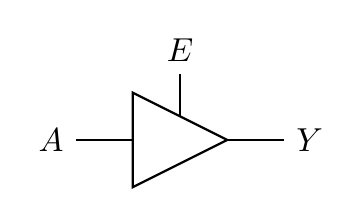
\begin{tikzpicture}[scale=1.2, transform shape]
    % Triangle for buffer
    \draw[thick] (0,0) -- (1,0.5) -- (0,1) -- cycle;
    % Input Line
    \draw[thick] (-0.6,0.5) -- (0,0.5) node[left, at start] {$A$};
    % Output Line
    \draw[thick] (1,0.5) -- (1.6,0.5) node[right] {$Y$};
    % Enable Line
    \draw[thick] (0.5,1.2) -- (0.5,0.75) node[above, at start] {$E$};
\end{tikzpicture}
\vspace{0.4cm}
\renewcommand{\arraystretch}{1.3}
\begin{tabular}{|c|c||c|c|}
\hline
\textbf{Enable ($E$)} & \textbf{Input ($A$)} & \textbf{Output ($Y$)} & \textbf{Operating State} \\
\hline
$0$ & $X$ (Don't Care) & $\mathbf{Z}$ & High-Impedance (Disconnected) \\
\hline
$1$ & $0$ & $\mathbf{0}$ & Logic Low (Active Drive) \\
\hline
$1$ & $1$ & $\mathbf{1}$ & Logic High (Active Drive) \\
\hline
\end{tabular}

\end{center}

\vspace{0.4cm}
\textbf{Advantages of Using Three-State Gates}

Three-state logic elements provide several critical structural and systemic benefits in modern digital architecture:

\begin{itemize}
    \item \textbf{Implementation of Shared Bus Architectures:} The foremost advantage of tri-state gates is their ability to connect multiple gate outputs to a single, common wire or communication bus. Under normal circumstances, connecting two standard gate outputs directly together is forbidden because if one outputs $1$ (high voltage) and the other outputs $0$ (low voltage), a damaging short-circuit occurs (known as bus contention). By ensuring that the control logic enables \textbf{only one tri-state gate at a time} while keeping all others disabled ($Z$), multiple components can safely share the same channel.
    
    \item \textbf{Bidirectional Data Transmission:} Tri-state gates allow a single physical pin or line to function both as an input and an output. This bidirectional capability is foundational for microprocessor data buses and memory interfaces (RAM/ROM modules), where data must be written to and read from the same location over the same wiring infrastructure.
    
    \item \textbf{Reduction in Routing Overhead and Area Optimization:} Without tri-state logic, multiplexing data from $N$ different registers would require large, multi-stage combinational multiplexing logic networks consisting of dozens of AND-OR gates. Tri-state gates allow multiplexing to occur right at the source directly onto the wire, eliminating excessive gating logic and drastically lowering routing complexity on modern silicon chips.
\end{itemize}

\vspace{0.3cm}
\textbf{Visualizing a Tri-State Shared Bus System}

The circuit diagram below demonstrates how two independent modules can safely drive a single shared bus line using mutual exclusion on their enable signals ($E_1 \cdot E_2 = 0$):

\begin{center}
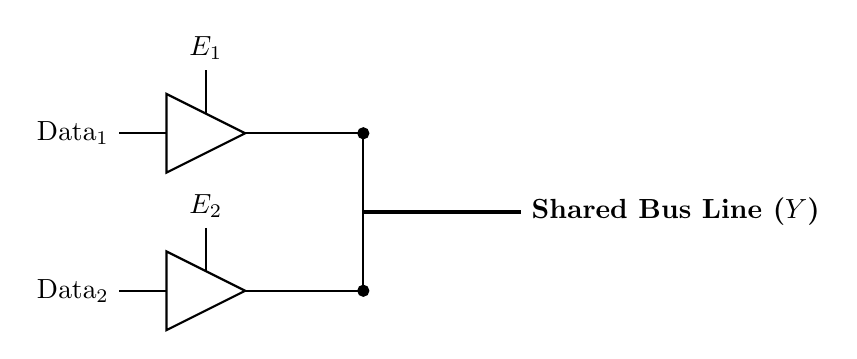
\begin{tikzpicture}[scale=1, transform shape]
    % Buffer 1
    \draw[thick] (0,1.5) -- (1,2) -- (0,2.5) -- cycle;
    \draw[thick] (-0.6,2) -- (0,2) node[left, at start] {$\text{Data}_1$};
    \draw[thick] (0.5,2.8) -- (0.5,2.25) node[above, at start] {$E_1$};
    \draw[thick] (1,2) -- (2.5,2) -- (2.5,1);
    
    % Buffer 2
    \draw[thick] (0,-0.5) -- (1,0) -- (0,0.5) -- cycle;
    \draw[thick] (-0.6,0) -- (0,0) node[left, at start] {$\text{Data}_2$};
    \draw[thick] (0.5,0.8) -- (0.5,0.25) node[above, at start] {$E_2$};
    \draw[thick] (1,0) -- (2.5,0) -- (2.5,1);

    % Common Bus
    \draw[very thick] (2.5,1) -- (4.5,1) node[right] {\textbf{Shared Bus Line ($Y$)}};
    \filldraw (2.5,2) circle (2pt);
    \filldraw (2.5,0) circle (2pt);
\end{tikzpicture}
\end{center}

\end{tcolorbox}

\item What do you mean by Universal gate? Show that both NAND gate and NOR gate are universal gates.
\mk{14} \yr{CSE 205 | L-2/T-1 | 2022--23, 2013--14} \variant{2019--20}

\begin{tcolorbox}[enhanced,breakable,ansbox,colback=cA!4,colframe=cA,boxrule=0.8pt,arc=5pt,title={\textbf{Answer}},fonttitle=\bfseries\color{white},colbacktitle=cA]

\textbf{1. Definition of a Universal Gate}

A \textbf{Universal Gate} is a logic gate that can be used to implement any Boolean function without requiring the use of any other type of logic gate. In digital logic design, any Boolean expression can be realized using a combination of the three fundamental logic gates: \textbf{NOT}, \textbf{AND}, and \textbf{OR}. 

Therefore, if we can demonstrate that a specific gate can successfully implement the NOT, AND, and OR operations purely by connecting multiple instances of itself, we prove that it is a universal gate. The two standard universal gates are the \textbf{NAND} gate and the \textbf{NOR} gate.

\vspace{0.5cm}
\textbf{2. Proof: NAND as a Universal Gate}

The NAND gate produces the complement of the logical product of its inputs: $Y = (A \cdot B)'$. We can construct the basic gates as follows:

\textbf{a) Implementing a NOT Gate using a NAND Gate}
To invert a signal, we apply the same input signal $A$ to all inputs of the NAND gate. According to the \textit{Idempotent Law} ($A \cdot A = A$), the operation simplifies to the logical complement.
\begin{align*}
    Y &= (A \cdot A)' \\
    Y &= A'
\end{align*}

\begin{center}
\begin{circuitikz}[scale=1, transform shape]
    \draw (0,0) node[nand port] (n1) {};
    % Input splitting with junction dot
    \draw (n1.in 1) -- ++(-0.3,0) coordinate (in1a);
    \draw (n1.in 2) -- ++(-0.3,0) coordinate (in2a);
    \draw (in1a) -- (in2a) coordinate[midway] (midA);
    \draw (midA) -- ++(-0.5,0) node[left] {$A$};
    \fill (midA) circle (1.5pt);
    
    \draw (n1.out) -- ++(0.5,0) node[right] {$Y = A'$};
\end{circuitikz}
\end{center}

\textbf{b) Implementing an AND Gate using NAND Gates}
An AND operation is simply a NAND operation followed by a NOT operation. Since we already know how to create a NOT gate using a NAND gate, we cascade two NAND gates.
\begin{align*}
    Y &= ((A \cdot B)')' \\
    \intertext{Using the \textit{Involution Law} $(X'') = X$:}
    Y &= A \cdot B
\end{align*}

\begin{center}
\begin{circuitikz}[scale=1, transform shape]
    \draw (0,0) node[nand port] (n1) {};
    \draw (3,0) node[nand port] (n2) {};
    
    \draw (n1.in 1) -- ++(-0.5,0) node[left] {$A$};
    \draw (n1.in 2) -- ++(-0.5,0) node[left] {$B$};
    
    % Connecting n1 output to both inputs of n2
    \draw (n1.out) -- ++(0.5,0) coordinate (junc1) node[above] {$(A \cdot B)'$};
    \draw (junc1) |- (n2.in 1);
    \draw (junc1) |- (n2.in 2);
    \fill (junc1) circle (1.5pt);
    
    \draw (n2.out) -- ++(0.5,0) node[right] {$Y = A \cdot B$};
\end{circuitikz}
\end{center}

\textbf{c) Implementing an OR Gate using NAND Gates}
To perform an OR operation, we first invert both inputs using NAND-based NOT gates, and then feed those inverted signals into a third NAND gate. We apply \textit{De Morgan's Theorem} to prove the equivalence.
\begin{align*}
    Y &= (A' \cdot B')' \\
    \intertext{Applying De Morgan's Law $(X \cdot Y)' = X' + Y'$:}
    Y &= (A')' + (B')' \\
    Y &= A + B
\end{align*}

\begin{center}
\begin{circuitikz}[scale=1, transform shape]
    \draw (0,1.2) node[nand port] (n1) {};
    \draw (0,-1.2) node[nand port] (n2) {};
    \draw (3,0) node[nand port] (n3) {};
    
    % A input splitting
    \draw (n1.in 1) -- ++(-0.3,0) coordinate (in1a);
    \draw (n1.in 2) -- ++(-0.3,0) coordinate (in2a);
    \draw (in1a) -- (in2a) coordinate[midway] (midA);
    \draw (midA) -- ++(-0.5,0) node[left] {$A$};
    \fill (midA) circle (1.5pt);
    
    % B input splitting
    \draw (n2.in 1) -- ++(-0.3,0) coordinate (in1b);
    \draw (n2.in 2) -- ++(-0.3,0) coordinate (in2b);
    \draw (in1b) -- (in2b) coordinate[midway] (midB);
    \draw (midB) -- ++(-0.5,0) node[left] {$B$};
    \fill (midB) circle (1.5pt);
    
    % Connecting n1 and n2 to n3
    \draw (n1.out) -- ++(0.5,0) node[midway, above] {$A'$} |- (n3.in 1);
    \draw (n2.out) -- ++(0.5,0) node[midway, below] {$B'$} |- (n3.in 2);
    
    \draw (n3.out) -- ++(0.5,0) node[right] {$Y = A + B$};
\end{circuitikz}
\end{center}

\rule{\textwidth}{0.4pt}
\vspace{0.3cm}

\textbf{3. Proof: NOR as a Universal Gate}

The NOR gate produces the complement of the logical sum of its inputs: $Y = (A + B)'$. The proofs follow a symmetric logic to the NAND gate implementations.

\textbf{a) Implementing a NOT Gate using a NOR Gate}
Applying the same input to all terminals of a NOR gate acts as an inverter. According to the \textit{Idempotent Law} ($A + A = A$).
\begin{align*}
    Y &= (A + A)' \\
    Y &= A'
\end{align*}

\begin{center}
\begin{circuitikz}[scale=1, transform shape]
    \draw (0,0) node[nor port] (n1) {};
    % Input splitting with junction dot
    \draw (n1.in 1) -- ++(-0.3,0) coordinate (in1a);
    \draw (n1.in 2) -- ++(-0.3,0) coordinate (in2a);
    \draw (in1a) -- (in2a) coordinate[midway] (midA);
    \draw (midA) -- ++(-0.5,0) node[left] {$A$};
    \fill (midA) circle (1.5pt);
    
    \draw (n1.out) -- ++(0.5,0) node[right] {$Y = A'$};
\end{circuitikz}
\end{center}

\textbf{b) Implementing an OR Gate using NOR Gates}
An OR operation is a NOR operation followed by an inversion (NOT gate created from a NOR gate).
\begin{align*}
    Y &= ((A + B)')' \\
    Y &= A + B
\end{align*}

\begin{center}
\begin{circuitikz}[scale=1, transform shape]
    \draw (0,0) node[nor port] (n1) {};
    \draw (3,0) node[nor port] (n2) {};
    
    \draw (n1.in 1) -- ++(-0.5,0) node[left] {$A$};
    \draw (n1.in 2) -- ++(-0.5,0) node[left] {$B$};
    
    % Connecting n1 output to both inputs of n2
    \draw (n1.out) -- ++(0.5,0) coordinate (junc1) node[above] {$(A + B)'$};
    \draw (junc1) |- (n2.in 1);
    \draw (junc1) |- (n2.in 2);
    \fill (junc1) circle (1.5pt);
    
    \draw (n2.out) -- ++(0.5,0) node[right] {$Y = A + B$};
\end{circuitikz}
\end{center}

\textbf{c) Implementing an AND Gate using NOR Gates}
To perform an AND operation, we invert both inputs using NOR gates, and then supply them to a third NOR gate. We prove this mathematically using \textit{De Morgan's Theorem}.
\begin{align*}
    Y &= (A' + B')' \\
    \intertext{Applying De Morgan's Law $(X + Y)' = X' \cdot Y'$:}
    Y &= (A')' \cdot (B')' \\
    Y &= A \cdot B
\end{align*}

\begin{center}
\begin{circuitikz}[scale=1, transform shape]
    \draw (0,1.2) node[nor port] (n1) {};
    \draw (0,-1.2) node[nor port] (n2) {};
    \draw (3,0) node[nor port] (n3) {};
    
    % A input splitting
    \draw (n1.in 1) -- ++(-0.3,0) coordinate (in1a);
    \draw (n1.in 2) -- ++(-0.3,0) coordinate (in2a);
    \draw (in1a) -- (in2a) coordinate[midway] (midA);
    \draw (midA) -- ++(-0.5,0) node[left] {$A$};
    \fill (midA) circle (1.5pt);
    
    % B input splitting
    \draw (n2.in 1) -- ++(-0.3,0) coordinate (in1b);
    \draw (n2.in 2) -- ++(-0.3,0) coordinate (in2b);
    \draw (in1b) -- (in2b) coordinate[midway] (midB);
    \draw (midB) -- ++(-0.5,0) node[left] {$B$};
    \fill (midB) circle (1.5pt);
    
    % Connecting n1 and n2 to n3
    \draw (n1.out) -- ++(0.5,0) node[midway, above] {$A'$} |- (n3.in 1);
    \draw (n2.out) -- ++(0.5,0) node[midway, below] {$B'$} |- (n3.in 2);
    
    \draw (n3.out) -- ++(0.5,0) node[right] {$Y = A \cdot B$};
\end{circuitikz}
\end{center}

\textbf{Conclusion:} Because we have successfully mapped the NOT, AND, and OR functional operators entirely to NAND gates and NOR gates, both are formally validated as universal logic gates.
\end{tcolorbox}

\item Show the circuit diagram of the expression $AB + CDE$ using only NAND gates.
\mk{10} \yr{CSE 205 | L-2/T-1 | 2021--22}

\begin{tcolorbox}[enhanced,breakable,ansbox,colback=cA!4,colframe=cA,boxrule=0.8pt,arc=5pt,title={\textbf{Answer}},fonttitle=\bfseries\color{white},colbacktitle=cA]

\textbf{1. Mathematical Derivation}

To implement a given Sum-of-Products (SOP) expression using only NAND gates, we must transform the expression into a form that exclusively uses the NAND operation ($(X \cdot Y)'$). We achieve this by applying double negation and De Morgan's laws.

Let the output function be $Y$:
\begin{align*}
Y &= AB + CDE & \text{(Original SOP expression)} \\
Y &= \left( (AB + CDE)' \right)' & \text{(Applying the Involution Law: $X = (X')'$)} \\
Y &= \left( (AB)' \cdot (CDE)' \right)' & \text{(Applying De Morgan's Law: $(X+Y)' = X' \cdot Y'$)}
\end{align*}

\textbf{Circuit Analysis:}
The resulting equation $Y = \left( (AB)' \cdot (CDE)' \right)'$ clearly defines a two-level NAND-NAND implementation:
\begin{itemize}
    \item \textbf{Level 1:} Two NAND gates generate the terms $(AB)'$ and $(CDE)'$. We will use a 2-input NAND gate for $AB$ and a 3-input NAND gate for $CDE$.
    \item \textbf{Level 2:} A final 2-input NAND gate takes the outputs from Level 1 and produces the target expression.
\end{itemize}

\vspace{0.5cm}
\textbf{2. Logic Circuit Diagram}

The circuit diagram below demonstrates the realization of the Boolean expression using standard 2-input and 3-input NAND gates.

\begin{center}
\begin{circuitikz}[scale=1.2, transform shape]
    % Level 1: First NAND gate (2-input) for (AB)'
    \node[nand port] (nand1) at (3, 2) {};
    \draw (nand1.in 1) -- ++(-1.5,0) node[left] {$A$};
    \draw (nand1.in 2) -- ++(-1.5,0) node[left] {$B$};
    
    % Level 1: Second NAND gate (3-input) for (CDE)'
    \node[nand port, number inputs=3] (nand2) at (3, -1) {};
    \draw (nand2.in 1) -- ++(-1.5,0) node[left] {$C$};
    \draw (nand2.in 2) -- ++(-1.5,0) node[left] {$D$};
    \draw (nand2.in 3) -- ++(-1.5,0) node[left] {$E$};
    
    % Level 2: Third NAND gate (2-input) for the final output
    \node[nand port] (nand3) at (6.5, 0.5) {};
    
    % Wiring from Level 1 to Level 2
    \draw (nand1.out) -- ++(1,0) |- (nand3.in 1);
    \draw (nand2.out) -- ++(1,0) |- (nand3.in 2);
    
    % Intermediate node labels
    \node[above] at (nand1.out) {$(AB)'$};
    \node[below] at (nand2.out) {$(CDE)'$};
    
    % Final output wiring
    \draw (nand3.out) -- ++(1,0) node[right] {$Y = AB + CDE$};
    
    % Add junction dots just for aesthetic alignment (optional here, but good practice if wires crossed)
\end{circuitikz}
\end{center}

\vspace{0.3cm}
\textit{Note:} If the design constraints strictly required only 2-input NAND gates, the 3-input NAND gate $(CDE)'$ would be expanded. We would first compute $(CD)'$, invert it using a NAND gate acting as a NOT gate to get $CD$, and then feed $CD$ and $E$ into another 2-input NAND gate to produce $(CDE)'$. However, 3-input NAND gates are standard components (e.g., the 7410 IC), so utilizing one directly provides the most optimal and generalized solution.

\end{tcolorbox}

\item A majority circuit is a combinational circuit whose output is equal to~1 if the input variables have more 1's than 0's, and 0 otherwise. Design a 3-input majority circuit by finding the circuit's truth table, simplified Boolean equation, and a logic diagram. Use only NAND gate(s) for your design.
\mk{18} \yr{CSE 205 | L-2/T-1 | 2019--20}



\begin{tcolorbox}[enhanced,breakable,ansbox,colback=cA!4,colframe=cA,boxrule=0.8pt,arc=5pt,title={\textbf{Answer}},fonttitle=\bfseries\color{white},colbacktitle=cA]

\section*{Design of a 3-Input Majority Circuit}

A majority circuit output is equal to 1 if the majority of its inputs are 1. For a 3-input combinational circuit with inputs $A$, $B$, and $C$, a majority occurs when two or more inputs are high ($\ge 2$).

---

\subsection*{1. Truth Table}
Based on the design criteria, the output $F$ is high for the minterms where the binary count of 1s is greater than or equal to 2. This corresponds to the minterms $m_3, m_5, m_6,$ and $m_7$.

\begin{center}
\begin{tabular}{ccccl}
\toprule
\multicolumn{3}{c}{\textbf{Inputs}} & \textbf{Output} & \\
\cmidrule(r){1-3} \cmidrule(l){4-4}
$A$ & $B$ & $C$ & $F$ & \textbf{Minterm} \\
\midrule
0 & 0 & 0 & 0 & $m_0$ \\
0 & 0 & 1 & 0 & $m_1$ \\
0 & 1 & 0 & 0 & $m_2$ \\
0 & 1 & 1 & 1 & $m_3 = \overline{A}BC$ \\
1 & 0 & 0 & 0 & $m_4$ \\
1 & 0 & 1 & 1 & $m_5 = A\overline{B}C$ \\
1 & 1 & 0 & 1 & $m_6 = AB\overline{C}$ \\
1 & 1 & 1 & 1 & $m_7 = ABC$ \\
\bottomrule
\end{tabular}
\end{center}

---

\subsection*{2. Boolean Simplification (Karnaugh Map)}
To find the simplified Sum-of-Products (SOP) expression, we map the 1s into a 3-variable Karnaugh Map:

\begin{center}
\begin{karnaugh-map}[4][2][1][$BC$][$A$]
    \minterms{3,5,6,7}
    \maxterms{0,1,2,4}
    \implicant{3}{7}
    \implicant{5}{7}
    \implicant{7}{6}
\end{karnaugh-map}
\end{center}

From the loops grouped above, we obtain three essential prime implicants:
\begin{itemize}
    \item Vertical loop grouping $m_3$ and $m_7$: $BC$
    \item Horizontal loop grouping $m_5$ and $m_7$: $AC$
    \item Bottom-right loop grouping $m_6$ and $m_7$: $AB$
\end{itemize}

Thus, the minimal SOP expression is:
\begin{equation*}
F = AB + BC + AC
\end{equation*}

---

\subsection*{3. Conversion to NAND-Only Logic}
To implement the circuit using exclusively NAND gates, we apply the Double Negation Law followed by De Morgan's Theorem to transform the SOP expression into a Product-of-Inversions format:

\begin{align*}
F &= AB + BC + AC \\
&= \overline{\overline{AB + BC + AC}} && \text{(Double Negation Law)} \\
&= \overline{\overline{AB} \cdot \overline{BC} \cdot \overline{AC}} && \text{(De Morgan's Law)}
\end{align*}

This final expression indicates that the circuit can be implemented using:
\begin{enumerate}
    \item Three 2-input NAND gates to generate $\overline{AB}$, $\overline{BC}$, and $\overline{AC}$.
    \item One 3-input NAND gate to combine the intermediate outputs.
\end{enumerate}

---

\subsection*{4. Logic Diagram}
The professional schematic below illustrates the NAND-only gate realization of the 3-input majority circuit.

\begin{center}
\begin{circuitikz}[scale=1.0, transform shape]
    % Draw vertical input rails
    \draw (0, 2.5) node[above] {$A$} -- (0, -2.5);
    \draw (0.8, 2.5) node[above] {$B$} -- (0.8, -2.5);
    \draw (1.6, 2.5) node[above] {$C$} -- (1.6, -2.5);
    
    % Place the three first-level 2-input NAND gates
    \node[nand port] (g1) at (4, 1.5) {};
    \node[nand port] (g2) at (4, 0) {};
    \node[nand port] (g3) at (4, -1.5) {};
    
    % Place the second-level 3-input NAND gate
    \node[nand port, number inputs=3] (gout) at (7, 0) {};
    
    % Connections for g1 (Inputs A and B)
    \draw (0,0 |- g1.in 1) to[short, *-] (g1.in 1);
    \draw (0.8,0 |- g1.in 2) to[short, *-] (g1.in 2);
    
    % Connections for g2 (Inputs B and C)
    \draw (0.8,0 |- g2.in 1) to[short, *-] (g2.in 1);
    \draw (1.6,0 |- g2.in 2) to[short, *-] (g2.in 2);
    
    % Connections for g3 (Inputs A and C)
    \draw (0,0 |- g3.in 1) to[short, *-] (g3.in 1);
    \draw (1.6,0 |- g3.in 2) to[short, *-] (g3.in 2);
    
    % Connections from first-level gates to output 3-input NAND gate
    \draw (g1.out) -- ++(0.6,0) |- (gout.in 1);
    \draw (g2.out) -- (gout.in 2);
    \draw (g3.out) -- ++(0.6,0) |- (gout.in 3);
    
    % Output Label
    \draw (gout.out) node[right] {$F$};
\end{circuitikz}
\end{center}

\end{tcolorbox}

\item Show that NAND gate is a universal logic gate. Also show that NAND operation does not follow the associative law.
\mk{5+5} \yr{CSE 205 | L-2/T-1 | 2015--16}

\begin{tcolorbox}[enhanced,breakable,ansbox,colback=cA!4,colframe=cA,boxrule=0.8pt,arc=5pt,title={\textbf{Answer}},fonttitle=\bfseries\color{white},colbacktitle=cA]

\section*{Part 1: Universality of the NAND Gate}

A logic gate is considered \textbf{universal} if it can be used to implement the three fundamental Boolean operations: \textbf{NOT}, \textbf{AND}, and \textbf{OR}. By demonstrating that a NAND gate can synthesize these three basic gates, we prove its universality. 

\subsection*{1. Implementing a NOT Gate}
A NOT gate (inverter) takes a single input $A$ and produces its complement $\overline{A}$. To achieve this using a 2-input NAND gate, we tie both inputs together.

\textbf{Boolean Derivation:}
\begin{align*}
F &= \text{NAND}(A, A) \\
F &= \overline{A \cdot A} && \text{(Definition of NAND)} \\
F &= \overline{A} && \text{(Idempotent Law: } A \cdot A = A \text{)}
\end{align*}

\textbf{Logic Diagram:}
\begin{center}
\begin{circuitikz}[scale=1.2, transform shape]
    \node[nand port] (n1) at (2,0) {};
    \draw (0,0) node[left] {$A$} -- (0.5,0);
    \draw (0.5,0) |- (n1.in 1);
    \draw (0.5,0) |- (n1.in 2);
    \fill (0.5,0) circle (1.5pt);
    \draw (n1.out) node[right] {$F = \overline{A}$};
\end{circuitikz}
\end{center}

\subsection*{2. Implementing an AND Gate}
An AND gate performs the Boolean product $A \cdot B$. Since a NAND gate produces $\overline{A \cdot B}$, we simply need to invert its output using a second NAND gate configured as a NOT gate.

\textbf{Boolean Derivation:}
\begin{align*}
F &= \text{NOT}(\text{NAND}(A, B)) \\
F &= \overline{(\overline{A \cdot B})} && \text{(Definition of NAND)} \\
F &= A \cdot B && \text{(Double Negation Law)}
\end{align*}

\textbf{Logic Diagram:}
\begin{center}
\begin{circuitikz}[scale=1.2, transform shape]
    \node[nand port] (n1) at (2,0) {};
    \node[nand port] (n2) at (5,0) {};
    
    \draw (n1.in 1) node[left] {$A$};
    \draw (n1.in 2) node[left] {$B$};
    
    \draw (n1.out) -- (3.5,0);
    \draw (3.5,0) |- (n2.in 1);
    \draw (3.5,0) |- (n2.in 2);
    \fill (3.5,0) circle (1.5pt);
    
    \draw (n2.out) node[right] {$F = A \cdot B$};
\end{circuitikz}
\end{center}

\subsection*{3. Implementing an OR Gate}
An OR gate performs the Boolean sum $A + B$. We can implement this by first inverting both inputs using NAND gates, and then passing those inverted signals into a third NAND gate.

\textbf{Boolean Derivation:}
\begin{align*}
F &= \text{NAND}(\text{NOT}(A), \text{NOT}(B)) \\
F &= \text{NAND}(\overline{A}, \overline{B}) && \text{(From NOT implementation)} \\
F &= \overline{\overline{A} \cdot \overline{B}} && \text{(Definition of NAND)} \\
F &= \overline{\overline{A}} + \overline{\overline{B}} && \text{(De Morgan's Law)} \\
F &= A + B && \text{(Double Negation Law)}
\end{align*}

\textbf{Logic Diagram:}
\begin{center}
\begin{circuitikz}[scale=1.2, transform shape]
    \node[nand port] (na) at (2,1) {};
    \node[nand port] (nb) at (2,-1) {};
    \node[nand port] (nout) at (5,0) {};
    
    % Input A
    \draw (0,1) node[left] {$A$} -- (0.5,1);
    \draw (0.5,1) |- (na.in 1);
    \draw (0.5,1) |- (na.in 2);
    \fill (0.5,1) circle (1.5pt);
    
    % Input B
    \draw (0,-1) node[left] {$B$} -- (0.5,-1);
    \draw (0.5,-1) |- (nb.in 1);
    \draw (0.5,-1) |- (nb.in 2);
    \fill (0.5,-1) circle (1.5pt);
    
    % Connections to final NAND
    \draw (na.out) node[above] {$\overline{A}$} -- (3.2,1) |- (nout.in 1);
    \draw (nb.out) node[below] {$\overline{B}$} -- (3.2,-1) |- (nout.in 2);
    
    \draw (nout.out) node[right] {$F = A + B$};
\end{circuitikz}
\end{center}

Because the NAND gate can implement NOT, AND, and OR functions, it is formally proven to be a \textbf{universal gate}.

\vspace{0.5cm}
\hrule
\vspace{0.5cm}

\section*{Part 2: Non-Associativity of the NAND Operation}

The associative law states that for a given binary operator $\uparrow$, the grouping of operands does not affect the result:
$$ (A \uparrow B) \uparrow C = A \uparrow (B \uparrow C) $$

Let the operator $\uparrow$ denote the NAND operation, where $A \uparrow B = \overline{A \cdot B}$. We will evaluate the Left-Hand Side (LHS) and Right-Hand Side (RHS) of the associative equation independently.

\textbf{Evaluating the Left-Hand Side (LHS):}
\begin{align*}
\text{LHS} &= (A \uparrow B) \uparrow C \\
&= (\overline{A \cdot B}) \uparrow C && \text{(Definition of NAND)} \\
&= \overline{(\overline{A \cdot B}) \cdot C} && \text{(Definition of NAND)} \\
&= \overline{(\overline{A \cdot B})} + \overline{C} && \text{(De Morgan's Law)} \\
&= (A \cdot B) + \overline{C} && \text{(Double Negation Law)}
\end{align*}

\textbf{Evaluating the Right-Hand Side (RHS):}
\begin{align*}
\text{RHS} &= A \uparrow (B \uparrow C) \\
&= A \uparrow (\overline{B \cdot C}) && \text{(Definition of NAND)} \\
&= \overline{A \cdot (\overline{B \cdot C})} && \text{(Definition of NAND)} \\
&= \overline{A} + \overline{(\overline{B \cdot C})} && \text{(De Morgan's Law)} \\
&= \overline{A} + (B \cdot C) && \text{(Double Negation Law)}
\end{align*}

Comparing the simplified expressions, we clearly see that:
$$ (A \cdot B) + \overline{C} \neq \overline{A} + (B \cdot C) $$

\textbf{Counterexample via Truth Values:}
To definitively prove the inequality, we can assign an arbitrary set of values, such as $A = 0$, $B = 0$, and $C = 1$.

\begin{itemize}
    \item \textbf{LHS:} $((0 \cdot 0) + \overline{1}) = (0 + 0) = \mathbf{0}$
    \item \textbf{RHS:} $(\overline{0} + (0 \cdot 1)) = (1 + 0) = \mathbf{1}$
\end{itemize}

Since $0 \neq 1$, the LHS and RHS do not yield the same result for the same input combination. Therefore, \textbf{the NAND operation does not follow the associative law.}

\end{tcolorbox}

\item Define: Odd Function, Even Function, Don't-care conditions.
\mk{5} \yr{CSE 205 | L-2/T-1 | 2013--14}

\begin{tcolorbox}[enhanced,breakable,ansbox,colback=cA!4,colframe=cA,boxrule=0.8pt,arc=5pt,title={\textbf{Answer}},fonttitle=\bfseries\color{white},colbacktitle=cA]

\section*{Definitions of Logic Function Properties}

\subsection*{1. Odd Function}
In digital logic, an \textbf{odd function} is a Boolean function that evaluates to logic $1$ if and only if an \textbf{odd number} of its input variables are equal to logic $1$. 
\begin{itemize}
    \item \textbf{Operation:} The multiple-input exclusive-OR (XOR) operation inherently implements an odd function.
    \item \textbf{Example (3-Variable):} $F_{\text{odd}}(A,B,C) = A \oplus B \oplus C = \sum m(1, 2, 4, 7)$
\end{itemize}

\subsection*{2. Even Function}
An \textbf{even function} is a Boolean function that evaluates to logic $1$ if and only if an \textbf{even number} of its input variables are equal to logic $1$. In binary logic, zero is considered an even number, so the function also outputs $1$ when all inputs are $0$.
\begin{itemize}
    \item \textbf{Operation:} For a $3$-variable system, the complement of the XOR function (which is the exclusive-NOR, or XNOR, evaluated sequentially) yields an even function.
    \item \textbf{Example (3-Variable):} $F_{\text{even}}(A,B,C) = (A \oplus B \oplus C)' = \sum m(0, 3, 5, 6)$
\end{itemize}

\vspace{0.3cm}
\textbf{Truth Table Comparison (3 Variables):}
\begin{center}
\begin{tabular}{ccccccc}
\toprule
\multicolumn{3}{c}{\textbf{Inputs}} & \textbf{Count} & \textbf{Odd Function} & \textbf{Even Function} & \\
\cmidrule(r){1-3}
$A$ & $B$ & $C$ & \textbf{of 1s} & $F = A \oplus B \oplus C$ & $F = (A \oplus B \oplus C)'$ & \textbf{Minterm} \\
\midrule
0 & 0 & 0 & 0 & \textbf{0} & \textbf{1} & $m_0$ \\
0 & 0 & 1 & 1 & \textbf{1} & \textbf{0} & $m_1$ \\
0 & 1 & 0 & 1 & \textbf{1} & \textbf{0} & $m_2$ \\
0 & 1 & 1 & 2 & \textbf{0} & \textbf{1} & $m_3$ \\
1 & 0 & 0 & 1 & \textbf{1} & \textbf{0} & $m_4$ \\
1 & 0 & 1 & 2 & \textbf{0} & \textbf{1} & $m_5$ \\
1 & 1 & 0 & 2 & \textbf{0} & \textbf{1} & $m_6$ \\
1 & 1 & 1 & 3 & \textbf{1} & \textbf{0} & $m_7$ \\
\bottomrule
\end{tabular}
\end{center}

\vspace{0.5cm}

\subsection*{3. Don't-Care Conditions}
In certain digital systems, specific input combinations may either never physically occur (e.g., states $1010$ to $1111$ in a BCD, Binary-Coded Decimal, system) or the system's output for those specific input combinations does not affect the overall circuit behavior. The unassigned output states for these combinations are defined as \textbf{don't-care conditions}.

\begin{itemize}
    \item \textbf{Notation:} They are typically denoted by \textbf{X}, \textbf{d}, or $\Phi$ in truth tables and Boolean expressions. For example: $F(A,B,C) = \sum m(0,1) + \sum d(2,3)$.
    \item \textbf{Application in Minimization:} During logic simplification (e.g., using Karnaugh Maps or the Quine-McCluskey algorithm), a designer can arbitrarily treat a don't-care condition as either a $1$ or a $0$. The strategic choice is to assign them the value that leads to the largest possible groupings (implicants), thereby yielding the most minimized and cost-effective logic circuit.
\end{itemize}

\textbf{Example of K-Map Optimization using Don't-Cares:}
Consider $F(A,B,C) = \sum m(0,1) + \sum d(2,3)$. Without don't-cares, $m_0$ and $m_1$ group to form $\overline{A}\overline{B}$. By treating the don't-cares ($d_2, d_3$) as $1$s, we can form a quad, simplifying the expression significantly to $F = \overline{A}$.

\begin{center}
\begin{karnaugh-map}[4][2][1][$BC$][$A$]
    \minterms{0,1}
    \indeterminants{2,3}
    \maxterms{4,5,6,7}
    \implicant{0}{3}
\end{karnaugh-map}
\end{center}

\end{tcolorbox}

\end{enumerate}

%%──────────────────────────────────────────────────────────────────────
\subtopic{cA}{Circuit Analysis}
\label{sub:s1-circuit-analysis}

\begin{enumerate}

\item Analyze the following circuit and determine the output $F$ as sum of minterms and product of maxterms.


\begin{center}
  \begin{circuitikz}[thick]
        % Gates
        \node[xnor port] (xnor) at (3, 2) {};
        \node[nand port] (nand) at (3, 0) {};
        \node[xor port] (xor) at (6, 1) {};

        % Input labels and connections to the left
        \node[left] at (-1, 2.28) {$A$};
        \draw (-1, 2.28) -- (xnor.in 1);
        
        \node[left] at (-1, 1) {$B$};
        \draw (-1, 1) -- (1, 1); % Main B line
        \draw (1, 1) |- (xnor.in 2); % B to XNOR
        \draw (1, 1) |- (nand.in 1); % B to NAND
        
        \node[left] at (-1, -0.28) {$C$};
        \draw (-1, -0.28) -- (nand.in 2);

        % Connect intermediate gates to final XOR gate
        \draw (xnor.out) -| (xor.in 1);
        \draw (nand.out) -| (xor.in 2);

        % Output F
        \draw (xor.out) -- ++(1.5,0) node[right] {$F$};
        
    \end{circuitikz}
\end{center}

\mk{9} \yr{CSE 205 | L-2/T-1 | 2011--12}

\begin{tcolorbox}[enhanced,breakable,ansbox,colback=cA!4,colframe=cA,boxrule=0.8pt,arc=5pt,title={\textbf{Answer}},fonttitle=\bfseries\color{white},colbacktitle=cA]

\section*{Circuit Analysis: Sum of Minterms and Product of Maxterms}

To determine the output $F$ in its canonical forms, we will first extract the Boolean expression from the logic circuit, simplify it algebraically, and verify the results using a Truth Table.

\subsection*{1. Boolean Expression Extraction}
Let us define the intermediate signals at the outputs of the first-stage gates as $X$ and $Y$.

\begin{center}
  \begin{circuitikz}[thick, scale=0.9, transform shape]
      % Gates
      \node[xnor port] (xnor) at (3, 2) {};
      \node[nand port] (nand) at (3, 0) {};
      \node[xor port] (xor) at (6, 1) {};

      % Input labels and connections
      \node[left] at (-1, 2.28) {$A$};
      \draw (-1, 2.28) -- (xnor.in 1);
      
      \node[left] at (-1, 1) {$B$};
      \draw (-1, 1) -- (1, 1); 
      \draw (1, 1) |- (xnor.in 2); 
      \draw (1, 1) |- (nand.in 1); 
      \fill (1,1) circle (2pt); % Junction dot
      
      \node[left] at (-1, -0.28) {$C$};
      \draw (-1, -0.28) -- (nand.in 2);

      % Intermediate labels
      \node[above] at (4.5, 2.2) {$X = A \odot B$};
      \node[below] at (4.5, -0.2) {$Y = \overline{BC}$};

      % Connect to XOR
      \draw (xnor.out) -| (xor.in 1);
      \draw (nand.out) -| (xor.in 2);

      % Output F
      \draw (xor.out) -- ++(1.5,0) node[right] {$F$};
  \end{circuitikz}
\end{center}

From the circuit diagram, we can write the equations for the intermediate nodes and the final output:
\begin{itemize}
    \item Top Gate (XNOR): $X = A \odot B$
    \item Bottom Gate (NAND): $Y = \overline{BC}$
    \item Output Gate (XOR): $F = X \oplus Y$
\end{itemize}

\subsection*{2. Algebraic Derivation}
Substitute $X$ and $Y$ into the XOR expression. By definition, $X \oplus Y = X\overline{Y} + \overline{X}Y$.

First, find the complements $\overline{X}$ and $\overline{Y}$:
\begin{align*}
    \overline{X} &= \overline{A \odot B} = A \oplus B = A\overline{B} + \overline{A}B \\
    \overline{Y} &= \overline{\overline{BC}} = BC && \text{(Double Negation Law)}
\end{align*}

Now, substitute $X$, $\overline{X}$, $Y$, and $\overline{Y}$ into the expression for $F$:
\begin{align*}
    F &= (A \odot B)(BC) + (A \oplus B)(\overline{BC}) \\
    F &= (AB + \overline{A}\overline{B})(BC) + (A\overline{B} + \overline{A}B)(\overline{B} + \overline{C}) && \text{(De Morgan's Law on } \overline{BC} \text{)}
\end{align*}

Expand both terms using the Distributive Law:
\begin{align*}
    \text{Term 1: } & (AB)(BC) + (\overline{A}\overline{B})(BC) \\
    &= ABC + \overline{A}(\overline{B}B)C && \text{(Idempotent Law: } BB=B \text{)} \\
    &= ABC + 0 && \text{(Complement Law: } \overline{B}B=0 \text{)} \\
    &= ABC
\end{align*}

\begin{align*}
    \text{Term 2: } & A\overline{B}\overline{B} + A\overline{B}\overline{C} + \overline{A}B\overline{B} + \overline{A}B\overline{C} \\
    &= A\overline{B} + A\overline{B}\overline{C} + 0 + \overline{A}B\overline{C} && \text{(Idempotent } \overline{B}\overline{B}=\overline{B} \text{, Complement } B\overline{B}=0 \text{)} \\
    &= A\overline{B}(1 + \overline{C}) + \overline{A}B\overline{C} && \text{(Factoring } A\overline{B} \text{)} \\
    &= A\overline{B}(1) + \overline{A}B\overline{C} && \text{(Identity Law: } 1+X=1 \text{)} \\
    &= A\overline{B} + \overline{A}B\overline{C}
\end{align*}

Combine the simplified terms:
\begin{equation*}
    F = ABC + A\overline{B} + \overline{A}B\overline{C}
\end{equation*}

To express $F$ as a sum of minterms, we expand the incomplete term ($A\overline{B}$) by multiplying it by $(C + \overline{C})$:
\begin{align*}
    F &= ABC + A\overline{B}(C + \overline{C}) + \overline{A}B\overline{C} \\
    F &= ABC + A\overline{B}C + A\overline{B}\overline{C} + \overline{A}B\overline{C}
\end{align*}

Translating the boolean products to their binary equivalents (where uncomplemented = 1, complemented = 0):
\begin{itemize}
    \item $ABC \rightarrow 111 = m_7$
    \item $A\overline{B}C \rightarrow 101 = m_5$
    \item $A\overline{B}\overline{C} \rightarrow 100 = m_4$
    \item $\overline{A}B\overline{C} \rightarrow 010 = m_2$
\end{itemize}

\subsection*{3. Truth Table Verification}
We construct a truth table to double-check the logic levels for all $8$ combinations of $A, B, C$.

\begin{center}
\begin{tabular}{cccccccc}
\toprule
\multicolumn{3}{c}{\textbf{Inputs}} & \textbf{XNOR} & \textbf{NAND} & \textbf{Output} & \multicolumn{2}{c}{\textbf{Canonical Forms}} \\
\cmidrule(r){1-3} \cmidrule(lr){4-4} \cmidrule(lr){5-5} \cmidrule(lr){6-6} \cmidrule(l){7-8}
$A$ & $B$ & $C$ & $X = A \odot B$ & $Y = \overline{BC}$ & $F = X \oplus Y$ & \textbf{Minterm} & \textbf{Maxterm} \\
\midrule
0 & 0 & 0 & 1 & 1 & \textbf{0} & & $M_0$ \\
0 & 0 & 1 & 1 & 1 & \textbf{0} & & $M_1$ \\
0 & 1 & 0 & 0 & 1 & \textbf{1} & $m_2$ & \\
0 & 1 & 1 & 0 & 0 & \textbf{0} & & $M_3$ \\
1 & 0 & 0 & 0 & 1 & \textbf{1} & $m_4$ & \\
1 & 0 & 1 & 0 & 1 & \textbf{1} & $m_5$ & \\
1 & 1 & 0 & 1 & 1 & \textbf{0} & & $M_6$ \\
1 & 1 & 1 & 1 & 0 & \textbf{1} & $m_7$ & \\
\bottomrule
\end{tabular}
\end{center}

\subsection*{4. Final Answer}
From both the algebraic derivation and the truth table, the function equals $1$ for minterms 2, 4, 5, and 7, and equals $0$ for maxterms 0, 1, 3, and 6. 

\vspace{0.3cm}
\noindent\textbf{Sum of Minterms ($\Sigma m$):}
\begin{equation*}
    F(A,B,C) = \sum m(2, 4, 5, 7)
\end{equation*}

\vspace{0.2cm}
\noindent\textbf{Product of Maxterms ($\Pi M$):}
\begin{equation*}
    F(A,B,C) = \prod M(0, 1, 3, 6)
\end{equation*}

\end{tcolorbox}

\end{enumerate}

%%──────────────────────────────────────────────────────────────────────
\subtopic{cA}{Two-Level \& Multi-Level Logic Implementation}
\label{sub:s1-two-level}

\begin{enumerate}

\item Simplify the following function and draw the circuit using only NAND gates:
\[ F(w,x,y,z) = \Sigma\,(0,1,2,4,5,6,8,9,12,13,14) \]
\mk{16} \yr{CSE 205 | L-2/T-1 | 2023--24}


\item Implement $F(x,y,z) = x'y'z' + xyz'$ using two-level forms of logic by using NAND-AND gates. Assume that the complement of $x$, $y$ and $z$ are readily available.
\mk{14} \yr{CSE 205 | L-2/T-1 | 2023--24}


\item Express $f(A,B,C,D) = \Sigma\,(0,4,8,9,10,11,12,14)$ with the two-level forms of logic ``NAND-AND'' and ``OR-NAND''.
\mk{6} \yr{CSE 205 | L-2/T-1 | 2018--19}

\begin{tcolorbox}[enhanced,breakable,ansbox,colback=cA!4,colframe=cA,boxrule=0.8pt,arc=5pt,title={\textbf{Answer}},fonttitle=\bfseries\color{white},colbacktitle=cA]

\section*{Two-Level Logic Design: NAND-AND and OR-NAND Forms}

To implement a logic function in specific two-level forms, we must first derive the simplified Boolean expressions for the function $f$ and its complement $f'$. We achieve this using Karnaugh Maps.

The given Boolean function is:
$$f(A,B,C,D) = \Sigma\,(0,4,8,9,10,11,12,14)$$

The unlisted minterms form the complement function $f'$:
$$f'(A,B,C,D) = \Sigma\,(1,2,3,5,6,7,13,15)$$

---

\subsection*{1. Karnaugh Map Simplification}

\textbf{Minimizing $\boldsymbol{f}$ (Sum of Products for $\boldsymbol{f}$):}
We plot the minterms of $f$ on a 4-variable K-Map to find the minimal Sum of Products (SOP).

\begin{center}
\begin{karnaugh-map}[4][4][1][$CD$][$AB$]
    \minterms{0,4,8,9,10,11,12,14}
    \maxterms{1,2,3,5,6,7,13,15}
    \implicant{0}{8}
    \implicant{8}{10}
    \implicantedge{12}{8}{14}{10}
\end{karnaugh-map}
\end{center}

From the groupings above, we extract three essential prime implicants:
\begin{itemize}
    \item Left column group $(0, 4, 12, 8)$: $C'D'$
    \item Bottom row group $(8, 9, 11, 10)$: $AB'$
    \item Wrapped edge quad $(12, 14, 8, 10)$: $AD'$
\end{itemize}
Thus, the simplified SOP expression for $f$ is:
\begin{equation}
    f = C'D' + AB' + AD'
\end{equation}

\vspace{0.5cm}

\textbf{Minimizing $\boldsymbol{f'}$ (Sum of Products for $\boldsymbol{f'}$):}
We plot the minterms of $f'$ to find its minimal SOP.

\begin{center}
\begin{karnaugh-map}[4][4][1][$CD$][$AB$]
    \minterms{1,2,3,5,6,7,13,15}
    \maxterms{0,4,8,9,10,11,12,14}
    \implicant{1}{7}
    \implicant{5}{15}
    \implicant{3}{6}
\end{karnaugh-map}
\end{center}

From the K-Map for $f'$, we obtain:
\begin{itemize}
    \item Group $(1, 3, 5, 7)$: $A'D$
    \item Group $(2, 3, 6, 7)$: $A'C$
    \item Group $(5, 7, 13, 15)$: $BD$
\end{itemize}
Thus, the simplified SOP expression for $f'$ is:
\begin{equation}
    f' = A'D + A'C + BD
\end{equation}

---

\subsection*{2. NAND-AND Logic Form}

The \textbf{NAND-AND} form requires the logic equation to be a product of inverted terms (First Level: NAND, Second Level: AND). We derive this naturally from the SOP of the complemented function $f'$.

By taking the complement of both sides of Equation (2):
\begin{align*}
    f &= (f')' \\
    f &= (A'D + A'C + BD)'
\end{align*}
Applying \textbf{De Morgan's Law} to distribute the inversion over the OR terms:
\begin{align*}
    f &= (A'D)' \cdot (A'C)' \cdot (BD)'
\end{align*}

This equation maps directly to a two-level NAND-AND circuit:

\begin{center}
\begin{circuitikz}[scale=1.0, transform shape, thick]
    % Inputs
    \node (Ap1) at (0, 3) {$A'$};
    \node (D1)  at (0, 2.5) {$D$};
    
    \node (Ap2) at (0, 1.5) {$A'$};
    \node (C)   at (0, 1) {$C$};
    
    \node (B)  at (0, 0) {$B$};
    \node (D2) at (0, -0.5) {$D$};

    % First Level: NAND Gates
    \node[nand port] (nand1) at (3, 2.75) {};
    \node[nand port] (nand2) at (3, 1.25) {};
    \node[nand port] (nand3) at (3, -0.25) {};

    % Connections to Level 1
    \draw (Ap1) -- (nand1.in 1);
    \draw (D1) -- (nand1.in 2);
    \draw (Ap2) -- (nand2.in 1);
    \draw (C) -- (nand2.in 2);
    \draw (B) -- (nand3.in 1);
    \draw (D2) -- (nand3.in 2);

    % Second Level: AND Gate
    \node[and port, number inputs=3] (and1) at (6.5, 1.25) {};

    % Connections to Level 2
    \draw (nand1.out) node[above right] {$(A'D)'$} -- ++(1,0) |- (and1.in 1);
    \draw (nand2.out) node[above right] {$(A'C)'$} -- (and1.in 2);
    \draw (nand3.out) node[below right] {$(BD)'$} -- ++(1,0) |- (and1.in 3);

    % Output
    \draw (and1.out) -- ++(0.5,0) node[right] {$f$};
\end{circuitikz}
\end{center}

---

\subsection*{3. OR-NAND Logic Form}

The \textbf{OR-NAND} form requires the logic equation to be an inverted product of sums (First Level: OR, Second Level: NAND). This is obtained by expressing $f'$ as a Product of Sums (POS), and then taking its complement.

The POS of $f'$ is the logical complement of the SOP of $f$ (Equation 1). Applying \textbf{De Morgan's Law} to Equation (1):
\begin{align*}
    f' &= (C'D' + AB' + AD')' \\
    f' &= (C+D) \cdot (A'+B) \cdot (A'+D) 
\end{align*}
To find $f$, we complement $f'$ again:
\begin{align*}
    f &= (f')' \\
    f &= \big( (C+D) \cdot (A'+B) \cdot (A'+D) \big)'
\end{align*}

This equation translates perfectly into a two-level OR-NAND circuit:

\begin{center}
\begin{circuitikz}[scale=1.0, transform shape, thick]
    % Inputs
    \node (C)  at (0, 3) {$C$};
    \node (D1) at (0, 2.5) {$D$};
    
    \node (Ap1) at (0, 1.5) {$A'$};
    \node (B)   at (0, 1) {$B$};
    
    \node (Ap2) at (0, 0) {$A'$};
    \node (D2)  at (0, -0.5) {$D$};

    % First Level: OR Gates
    \node[or port] (or1) at (3, 2.75) {};
    \node[or port] (or2) at (3, 1.25) {};
    \node[or port] (or3) at (3, -0.25) {};

    % Connections to Level 1
    \draw (C) -- (or1.in 1);
    \draw (D1) -- (or1.in 2);
    \draw (Ap1) -- (or2.in 1);
    \draw (B) -- (or2.in 2);
    \draw (Ap2) -- (or3.in 1);
    \draw (D2) -- (or3.in 2);

    % Second Level: NAND Gate
    \node[nand port, number inputs=3] (nand1) at (6.5, 1.25) {};

    % Connections to Level 2
    \draw (or1.out) node[above right] {$C+D$} -- ++(1,0) |- (nand1.in 1);
    \draw (or2.out) node[above right] {$A'+B$} -- (nand1.in 2);
    \draw (or3.out) node[below right] {$A'+D$} -- ++(1,0) |- (nand1.in 3);

    % Output
    \draw (nand1.out) -- ++(0.5,0) node[right] {$f$};
\end{circuitikz}
\end{center}

\end{tcolorbox}

\item Implement the function $F(w, x, y, z) = w'x' + w'x'z + w'yz'$ using two-level forms of logic by
\begin{enumerate}
  \item NOR gates only
  \item AND-NOR
  \item NAND gates only
  \item OR-NAND
\end{enumerate}
\mk{20} \yr{CSE 205 | L-2/T-1 | 2014--15}

\begin{tcolorbox}[enhanced,breakable,ansbox,colback=cA!4,colframe=cA,boxrule=0.8pt,arc=5pt,title={\textbf{Answer}},fonttitle=\bfseries\color{white},colbacktitle=cA]

\section*{Simplification and Two-Level Logic Implementations}

First, we simplify the given Boolean function $F(w, x, y, z)$ to its minimal Sum of Products (SOP) form. This will serve as the foundation for our derivations.

\begin{align*}
F &= w'x' + w'x'z + w'yz' \\
F &= w'x'(1 + z) + w'yz' && \text{(Distributive Law)} \\
F &= w'x'(1) + w'yz' && \text{(Null Element Law: } 1 + X = 1 \text{)} \\
F &= w'x' + w'yz' && \text{(Identity Law: } X \cdot 1 = X \text{)}
\end{align*}

\vspace{0.3cm}
\hrule
\vspace{0.3cm}

\subsection*{1. NOR Gates Only (NOR-NOR Form)}
A two-level NOR-NOR circuit requires the function to be in the form of a complemented sum of negated sums. This is derived from the Product of Sums (POS) form of $F$.

\textbf{Step 1: Find the POS of $\boldsymbol{F}$}
\begin{align*}
F &= w'x' + w'yz' \\
F &= w'(x' + yz') && \text{(Distributive Law)} \\
F &= w'(x' + y)(x' + z') && \text{(Distributive Law: } A+BC = (A+B)(A+C) \text{)}
\end{align*}

\textbf{Step 2: Convert to NOR-NOR logic}
\begin{align*}
F &= \overline{\overline{w'(x' + y)(x' + z')}} && \text{(Double Negation Law)} \\
F &= \overline{w + (x' + y)' + (x' + z')'} && \text{(De Morgan's Law)}
\end{align*}

\begin{center}
\begin{circuitikz}[thick]
    \node[nor port] (nor1) at (3, 1.5) {};
    \node[nor port] (nor2) at (3, -1.5) {};
    \node[nor port, number inputs=3] (nor3) at (6, 0) {};

    \draw (nor1.in 1) -- ++(-1,0) node[left] {$x'$};
    \draw (nor1.in 2) -- ++(-1,0) node[left] {$y$};

    \draw (nor2.in 1) -- ++(-1,0) node[left] {$x'$};
    \draw (nor2.in 2) -- ++(-1,0) node[left] {$z'$};

    \draw (nor1.out) node[above right] {$(x'+y)'$} -- ++(0.5,0) |- (nor3.in 1);
    \draw (nor3.in 2) -- ++(-4.5,0) node[left] {$w$};
    \draw (nor2.out) node[below right] {$(x'+z')'$} -- ++(0.5,0) |- (nor3.in 3);

    \draw (nor3.out) -- ++(0.5,0) node[right] {$F$};
\end{circuitikz}
\end{center}

\vspace{0.3cm}
\hrule
\vspace{0.3cm}

\subsection*{2. AND-NOR Form}
A two-level AND-NOR circuit is structurally equivalent to the complement of the SOP of $F'$. Therefore, we first find the SOP of the complemented function $F'$.

\textbf{Step 1: Find the SOP of $\boldsymbol{F'}$}
\begin{align*}
F' &= (w'(x' + y)(x' + z'))' && \text{(Complementing the POS of } F \text{)} \\
F' &= w + (x' + y)' + (x' + z')' && \text{(De Morgan's Law)} \\
F' &= w + xy' + xz && \text{(De Morgan's Law and Double Negation)}
\end{align*}

\textbf{Step 2: Express $\boldsymbol{F}$ as an AND-NOR equation}
\begin{align*}
F &= (F')' \\
F &= \overline{w + xy' + xz} && \text{(Substitution)}
\end{align*}

\begin{center}
\begin{circuitikz}[thick]
    \node[and port] (and1) at (3, 1.5) {};
    \node[and port] (and2) at (3, -1.5) {};
    \node[nor port, number inputs=3] (nor) at (6, 0) {};

    \draw (and1.in 1) -- ++(-1,0) node[left] {$x$};
    \draw (and1.in 2) -- ++(-1,0) node[left] {$y'$};

    \draw (and2.in 1) -- ++(-1,0) node[left] {$x$};
    \draw (and2.in 2) -- ++(-1,0) node[left] {$z$};

    \draw (and1.out) node[above right] {$xy'$} -- ++(0.5,0) |- (nor.in 1);
    \draw (nor.in 2) -- ++(-4.5,0) node[left] {$w$};
    \draw (and2.out) node[below right] {$xz$} -- ++(0.5,0) |- (nor.in 3);

    \draw (nor.out) -- ++(0.5,0) node[right] {$F$};
\end{circuitikz}
\end{center}

\vspace{0.3cm}
\hrule
\vspace{0.3cm}

\subsection*{3. NAND Gates Only (NAND-NAND Form)}
A two-level NAND-NAND circuit translates directly from the SOP form of $F$. 

\textbf{Step 1: Start with SOP of $\boldsymbol{F}$}
\begin{equation*}
F = w'x' + w'yz'
\end{equation*}

\textbf{Step 2: Convert to NAND-NAND logic}
\begin{align*}
F &= \overline{\overline{w'x' + w'yz'}} && \text{(Double Negation Law)} \\
F &= \overline{(w'x')' \cdot (w'yz')'} && \text{(De Morgan's Law)}
\end{align*}

\begin{center}
\begin{circuitikz}[thick]
    \node[nand port] (nand1) at (3, 1.5) {};
    \node[nand port, number inputs=3] (nand2) at (3, -1.5) {};
    \node[nand port] (nand3) at (6, 0) {};

    \draw (nand1.in 1) -- ++(-1,0) node[left] {$w'$};
    \draw (nand1.in 2) -- ++(-1,0) node[left] {$x'$};

    \draw (nand2.in 1) -- ++(-1,0) node[left] {$w'$};
    \draw (nand2.in 2) -- ++(-1,0) node[left] {$y$};
    \draw (nand2.in 3) -- ++(-1,0) node[left] {$z'$};

    \draw (nand1.out) node[above right] {$(w'x')'$} -- ++(0.5,0) |- (nand3.in 1);
    \draw (nand2.out) node[below right] {$(w'yz')'$} -- ++(0.5,0) |- (nand3.in 2);

    \draw (nand3.out) -- ++(0.5,0) node[right] {$F$};
\end{circuitikz}
\end{center}

\vspace{0.3cm}
\hrule
\vspace{0.3cm}

\subsection*{4. OR-NAND Form}
A two-level OR-NAND circuit corresponds to the inversion of the POS form of $F'$. We must derive the POS of the complement function.

\textbf{Step 1: Find the POS of $\boldsymbol{F'}$}
Using the SOP of $F'$ determined previously ($F' = w + xy' + xz$):
\begin{align*}
F' &= w + x(y' + z) && \text{(Distributive Law)} \\
F' &= (w + x)(w + y' + z) && \text{(Distributive Law: } A+BC = (A+B)(A+C) \text{)}
\end{align*}

\textbf{Step 2: Express $\boldsymbol{F}$ as an OR-NAND equation}
\begin{align*}
F &= (F')' \\
F &= \overline{(w + x)(w + y' + z)} && \text{(Substitution)}
\end{align*}

\begin{center}
\begin{circuitikz}[thick]
    \node[or port] (or1) at (3, 1.5) {};
    \node[or port, number inputs=3] (or2) at (3, -1.5) {};
    \node[nand port] (nand) at (6, 0) {};

    \draw (or1.in 1) -- ++(-1,0) node[left] {$w$};
    \draw (or1.in 2) -- ++(-1,0) node[left] {$x$};

    \draw (or2.in 1) -- ++(-1,0) node[left] {$w$};
    \draw (or2.in 2) -- ++(-1,0) node[left] {$y'$};
    \draw (or2.in 3) -- ++(-1,0) node[left] {$z$};

    \draw (or1.out) node[above right] {$w+x$} -- ++(0.5,0) |- (nand.in 1);
    \draw (or2.out) node[below right] {$w+y'+z$} -- ++(0.5,0) |- (nand.in 2);

    \draw (nand.out) -- ++(0.5,0) node[right] {$F$};
\end{circuitikz}
\end{center}

\end{tcolorbox}

\item Show the truth table for the following function:
\[ F(x, y, z) = (x+y+z)(x+y+z')(x+y'+z)(x'+y+z) \]
\mk{8} \yr{CSE 205 | L-2/T-1 | 2014--15}

\begin{tcolorbox}[enhanced,breakable,ansbox,colback=cA!4,colframe=cA,boxrule=0.8pt,arc=5pt,title={\textbf{Answer}},fonttitle=\bfseries\color{white},colbacktitle=cA]

\section*{Truth Table Derivation}

The given Boolean function is presented in its canonical \textbf{Product of Sums (POS)} form:
\[ F(x, y, z) = (x+y+z)(x+y+z')(x+y'+z)(x'+y+z) \]

In a POS expression, each sum term is called a \textbf{maxterm} ($M_i$). A maxterm evaluates to logic $0$ for exactly one combination of the input variables. To determine the binary value of each maxterm, we map uncomplemented variables to $0$ and complemented variables to $1$. 

Let us evaluate each term to identify its corresponding row in the truth table where the function outputs a $0$:
\begin{align*}
    (x + y + z)   &\implies 000_2 \implies M_0 \\
    (x + y + z')  &\implies 001_2 \implies M_1 \\
    (x + y' + z)  &\implies 010_2 \implies M_2 \\
    (x' + y + z)  &\implies 100_2 \implies M_4
\end{align*}

Thus, the function can be compactly written using the Pi-notation for maxterms:
\[ F(x, y, z) = \Pi\,(0, 1, 2, 4) \]

This analysis establishes that the function $F$ will output \textbf{0} for the decimal input combinations 0, 1, 2, and 4. For all remaining input combinations (3, 5, 6, and 7), the function will output \textbf{1}.

\vspace{0.5cm}

\subsection*{Truth Table}

Constructing the table based on our derived maxterms:

\begin{center}
\renewcommand{\arraystretch}{1.2}
\begin{tabular}{ccc|cc}
    \toprule
    \textbf{Decimal ($i$)} & \textbf{$x$} & \textbf{$y$} & \textbf{$z$} & \textbf{$F(x,y,z)$} \\
    \midrule
    0 & 0 & 0 & 0 & \textcolor{cA}{\textbf{0}} \\
    1 & 0 & 0 & 1 & \textcolor{cA}{\textbf{0}} \\
    2 & 0 & 1 & 0 & \textcolor{cA}{\textbf{0}} \\
    3 & 0 & 1 & 1 & 1 \\
    4 & 1 & 0 & 0 & \textcolor{cA}{\textbf{0}} \\
    5 & 1 & 0 & 1 & 1 \\
    6 & 1 & 1 & 0 & 1 \\
    7 & 1 & 1 & 1 & 1 \\
    \bottomrule
\end{tabular}
\end{center}

\end{tcolorbox}

\item Given function $F = A'B + BC + AC$:
\begin{enumerate}
  \item Implement $F$ using AND, OR and NOT gates.
  \item Minimize $F$ in SOP form using K-Map.
  \item Implement the minimized $F$ using only NAND gates.

\end{enumerate}
\mk{15} \yr{CSE 205 | L-2/T-1 | 2013--14}

\begin{tcolorbox}[enhanced,breakable,ansbox,colback=cA!4,colframe=cA,boxrule=0.8pt,arc=5pt,title={\textbf{Answer}},fonttitle=\bfseries\color{white},colbacktitle=cA]

\section*{Logic Circuit Design and Minimization}

Given the Boolean function:
\[ F(A, B, C) = A'B + BC + AC \]

\vspace{0.3cm}
\hrule
\vspace{0.3cm}

\subsection*{1. Implementation using AND, OR, and NOT gates}

To implement the unminimized function $F$, we analyze its structure:
\begin{itemize}
    \item One \textbf{NOT} gate is required to generate the complement of $A$ ($A'$).
    \item Three 2-input \textbf{AND} gates are required to generate the product terms $A'B$, $BC$, and $AC$.
    \item One 3-input \textbf{OR} gate is required to sum the product terms together.
\end{itemize}

\begin{center}
\begin{circuitikz}[american, thick , x=1.4cm]
    % ১. ইনপুট রেল (A, B, C) তৈরি করা
    \draw (-1.5, 4.5) node[above] {$A$} -- (-1.5, -0.5);
    \draw (-1.0, 4.5) node[above] {$B$} -- (-1.0, -0.5);
    \draw (-0.5, 4.5) node[above] {$C$} -- (-0.5, -0.5);

    % ২. AND গেটগুলোর পজিশন ঠিক করা
    \node[american and port] (and1) at (3, 3.5) {};
    \node[american and port] (and2) at (3, 1.75) {};
    \node[american and port] (and3) at (3, 0) {};

    % ৩. A' এর জন্য NOT গেটটি স্থাপন করা (and1.in 1 এর সাথে সোজা করে)
    \node[american not port, anchor=out] (notA) at ([xshift=-0.8cm]and1.in 1) {};

    % ৪. ৩-ইনপুটের OR গেট স্থাপন করা (and2.out এর সাথে সোজা করে)
    \node[american or port, number inputs=3, anchor=in 2] (or) at ([xshift=1.5cm]and2.out) {};

    % ৫. ইনপুট রেল থেকে গেটগুলোতে কানেকশন দেওয়া
    % Rail A থেকে NOT গেটের ইনপুটে কানেকশন
    \draw (notA.in 1) -- (-1.5, 0 |- notA.in 1) node[circ] {};
    
    % NOT গেটের আউটপুট থেকে AND1 এর ১ম ইনপুটে কানেকশন
    \draw (notA.out) -- (and1.in 1);
    
    % Rail B থেকে AND1 এর ২য় ইনপুটে কানেকশন
    \draw (and1.in 2) -- (-1.0, 0 |- and1.in 2) node[circ] {};

    % Rail B থেকে AND2 এর ১ম ইনপুটে কানেকশন
    \draw (and2.in 1) -- (-1.0, 0 |- and2.in 1) node[circ] {};
    
    % Rail C থেকে AND2 এর ২য় ইনপুটে কানেকশন
    \draw (and2.in 2) -- (-0.5, 0 |- and2.in 2) node[circ] {};

    % Rail A থেকে AND3 এর ১ম ইনপুটে কানেকশন
    \draw (and3.in 1) -- (-1.5, 0 |- and3.in 1) node[circ] {};
    
    % Rail C থেকে AND3 এর ২য় ইনপুটে কানেকশন
    \draw (and3.in 2) -- (-0.5, 0 |- and3.in 2) node[circ] {};

    % ৬. AND গেটগুলোর আউটপুট OR গেটের ইনপুটে কানেক্ট করা
    \draw (and1.out) |- (or.in 1);
    \draw (and2.out) -- (or.in 2);
    \draw (and3.out) |- (or.in 3);

    % ৭. ফাইনাল আউটপুট লেবেল
    \draw (or.out) -- ([xshift=0.6cm]or.out) node[right] {$F(A, B, C)$};
\end{circuitikz}

\end{center}

\vspace{0.3cm}
\hrule
\vspace{0.3cm}

\subsection*{2. K-Map Minimization in SOP Form}

To plot the function on a Karnaugh Map, we first expand the terms into canonical minterms (Sum of Minterms) by introducing missing variables:
\begin{align*}
    A'B &= A'B(C + C') = A'BC + A'BC' \implies m_3 + m_2 \\
    BC &= (A + A')BC = ABC + A'BC \implies m_7 + m_3 \\
    AC &= A(B + B')C = ABC + AB'C \implies m_7 + m_5
\end{align*}
Thus, the canonical function is $F(A, B, C) = \Sigma m(2, 3, 5, 7)$. Let us map these $1$s onto a 3-variable K-Map.

\begin{center}
\begin{karnaugh-map}[4][2][1][$BC$][$A$]
    \minterms{2,3,5,7}
    \maxterms{0,1,4,6}
    \implicant{3}{2}
    \implicant{5}{7}
\end{karnaugh-map}
\end{center}

\textbf{Group Extraction:}
\begin{itemize}
    \item \textbf{Group 1} (Cells 2, 3): This horizontal pair yields the term \textcolor{cA}{$\mathbf{A'B}$}.
    \item \textbf{Group 2} (Cells 5, 7): This horizontal pair yields the term \textcolor{cA}{$\mathbf{AC}$}.
\end{itemize}
Notice that cells 3 and 7 form a vertical pair ($BC$), but this is a \textit{redundant group} since all its $1$s are already covered by essential prime implicants. This visual redundancy perfectly illustrates the \textbf{Consensus Theorem}.

The minimized SOP function is:
\begin{equation*}
    F_{\text{min}} = A'B + AC
\end{equation*}

\vspace{0.3cm}
\hrule
\vspace{0.3cm}

\subsection*{3. Implementation of Minimized $F$ using only NAND gates}

To construct the circuit using strictly NAND gates, we must convert the minimized SOP expression into a NAND-NAND form. We achieve this by applying the \textbf{Double Negation Law} and \textbf{De Morgan's Laws}:

\begin{align*}
    F_{\text{min}} &= A'B + AC \\
    F_{\text{min}} &= \overline{\overline{A'B + AC}} && \text{(Double Negation Law)} \\
    F_{\text{min}} &= \overline{\overline{(A'B)} \cdot \overline{(AC)}} && \text{(De Morgan's Law: } \overline{X+Y} = \overline{X}\cdot\overline{Y} \text{)}
\end{align*}

This equation dictates a two-level NAND structure:
\begin{enumerate}
    \item The first level generates the terms $\overline{A'B}$ and $\overline{AC}$. Note that $A'$ must also be created by tying the inputs of a NAND gate together (since $\overline{A \cdot A} = A'$).
    \item The second level NAND gate takes these inverted products and produces the final output $F$.
\end{enumerate}

\begin{center}
\begin{circuitikz}[thick]
    % NAND Gates
    \node[nand port] (invA) at (2, 3.5) {};
    \node[nand port] (nand1) at (5, 3) {};
    \node[nand port] (nand2) at (5, 1) {};
    \node[nand port] (nand3) at (8, 2) {};

    % Inputs A, B, C
    \draw (0, 3.5) node[left] {$A$} -- ++(0.5,0) node[circle,fill,inner sep=1.5pt](a_split1){} |- (invA.in 1);
    \draw (a_split1) |- (invA.in 2);
    
    \draw (0, 2.72) node[left] {$B$} -- (nand1.in 2);
    
    \draw (0, 0.72) node[left] {$C$} -- (nand2.in 2);

    % Wiring inside
    \draw (invA.out) |- (nand1.in 1);
    \draw (0, 3.5) ++(0.5,0) |- (nand2.in 1);

    % Output Stage
    \draw (nand1.out) node[above right] {$\overline{A'B}$} |- (nand3.in 1);
    \draw (nand2.out) node[above right] {$\overline{AC}$} |- (nand3.in 2);

    % Final
    \draw (nand3.out) -- ++(1,0) node[right] {$F$};
\end{circuitikz}
\end{center}

\end{tcolorbox}

\item Given the Boolean function $F = xy + x'y' + y'z$, implement it with (i) AND, OR and NOT gates, and (ii) only NAND gates.
\mk{5+5} \yr{CSE 205 | L-2/T-1 | 2012--13}

\begin{tcolorbox}[enhanced,breakable,ansbox,colback=cA!4,colframe=cA,boxrule=0.8pt,arc=5pt,title={\textbf{Answer}},fonttitle=\bfseries\color{white},colbacktitle=cA]

\section*{Logic Circuit Implementations}

We are given the Boolean function in Sum of Products (SOP) form:
\[ F(x, y, z) = xy + x'y' + y'z \]

\vspace{0.2cm}
\hrule
\vspace{0.4cm}

\subsection*{(i) Implementation using AND, OR, and NOT gates}

To implement $F$ directly using standard logic gates, we require:
\begin{itemize}
    \item \textbf{NOT Gates:} To generate the complements $x'$ and $y'$.
    \item \textbf{AND Gates:} Three 2-input AND gates to compute the product terms $(xy)$, $(x'y')$, and $(y'z)$.
    \item \textbf{OR Gate:} One 3-input OR gate to sum the product terms together.
\end{itemize}

\begin{center}
\begin{circuitikz}[thick, scale=0.9, transform shape]
    % NOT Gates
    \node[not port] (notX) at (3, 4.5) {};
    \node[not port] (notY) at (3, 2.5) {};
    
    % AND Gates
    \node[and port] (and1) at (6.5, 5) {};
    \node[and port] (and2) at (6.5, 3) {};
    \node[and port] (and3) at (6.5, 1) {};
    
    % OR Gate
    \node[or port, number inputs=3] (or1) at (9.5, 3) {};

    % Input definitions and basic wiring
    \draw (0, 5.28) node[left] {$x$} -- ++(1,0) coordinate(x_branch) -- (and1.in 1);
    \draw (x_branch) |- (notX.in);
    \fill (x_branch) circle (1.5pt);
    
    \draw (0, 4.72) node[left] {$y$} -- ++(0.5,0) coordinate(y_branch) |- (and1.in 2);
    \draw (y_branch) |- (notY.in);
    \fill (y_branch) circle (1.5pt);

    % Wiring complements to AND gates
    \draw (notX.out) |- (and2.in 1);
    
    \draw (notY.out) -- ++(0.5,0) coordinate(ybar_branch) |- (and2.in 2);
    \draw (ybar_branch) |- (and3.in 1);
    \fill (ybar_branch) circle (1.5pt);

    % Z input wiring
    \draw (0, 0.72) node[left] {$z$} -- ++(4.5,0) |- (and3.in 2);
    
    % Connecting to OR gate
    \draw (and1.out) node[above right] {$xy$} |- (or1.in 1);
    \draw (and2.out) node[above right] {$x'y'$} -- (or1.in 2);
    \draw (and3.out) node[above right] {$y'z$} |- (or1.in 3);
    
    % Final output
    \draw (or1.out) -- ++(1,0) node[right] {$F$};
\end{circuitikz}
\end{center}

\vspace{0.4cm}
\hrule
\vspace{0.4cm}

\subsection*{(ii) Implementation using ONLY NAND gates}

To implement the circuit exclusively with NAND gates, we must convert the SOP expression into a \textbf{NAND-NAND} structure. We achieve this by applying the \textit{Double Negation Law} and \textit{De Morgan's Laws}:

\begin{align*}
    F &= xy + x'y' + y'z \\
    F &= \overline{\overline{xy + x'y' + y'z}} && \text{(Double Negation Law)} \\
    F &= \overline{\overline{(xy)} \cdot \overline{(x'y')} \cdot \overline{(y'z)}} && \text{(De Morgan's Law: } \overline{A+B+C} = \overline{A}\cdot\overline{B}\cdot\overline{C}\text{)}
\end{align*}

This equation dictates a two-level NAND structure. Additionally, the complements $x'$ and $y'$ must be generated using NAND gates with their inputs tied together (since $\overline{A \cdot A} = A'$).

\begin{center}
\begin{circuitikz}[thick, scale=0.9, transform shape]
    % NAND Gates acting as NOTs
    \node[nand port] (invX) at (3, 4.5) {};
    \node[nand port] (invY) at (3, 2.5) {};
    
    % First Level NAND Gates
    \node[nand port] (nand1) at (6.5, 5) {};
    \node[nand port] (nand2) at (6.5, 3) {};
    \node[nand port] (nand3) at (6.5, 1) {};
    
    % Second Level (Output) NAND Gate
    \node[nand port, number inputs=3] (nandOut) at (9.5, 3) {};

    % X Input and tied split
    \draw (0, 5.28) node[left] {$x$} -- ++(1,0) coordinate(x_branch) -- (nand1.in 1);
    \draw (x_branch) |- (1.5, 4.5) coordinate(tieX);
    \fill (x_branch) circle (1.5pt);
    \fill (tieX) circle (1.5pt);
    \draw (tieX) |- (invX.in 1);
    \draw (tieX) |- (invX.in 2);
    
    % Y Input and tied split
    \draw (0, 4.72) node[left] {$y$} -- ++(0.5,0) coordinate(y_branch) |- (nand1.in 2);
    \draw (y_branch) |- (1.5, 2.5) coordinate(tieY);
    \fill (y_branch) circle (1.5pt);
    \fill (tieY) circle (1.5pt);
    \draw (tieY) |- (invY.in 1);
    \draw (tieY) |- (invY.in 2);

    % Wiring generated complements
    \draw (invX.out) |- (nand2.in 1);
    
    \draw (invY.out) -- ++(0.5,0) coordinate(ybar_branch) |- (nand2.in 2);
    \draw (ybar_branch) |- (nand3.in 1);
    \fill (ybar_branch) circle (1.5pt);

    % Z input wiring
    \draw (0, 0.72) node[left] {$z$} -- ++(4.5,0) |- (nand3.in 2);
    
    % First Level NAND to Output NAND
    \draw (nand1.out) node[above right] {$\overline{xy}$} |- (nandOut.in 1);
    \draw (nand2.out) node[above right] {$\overline{x'y'}$} -- (nandOut.in 2);
    \draw (nand3.out) node[above right] {$\overline{y'z}$} |- (nandOut.in 3);
    
    % Final output
    \draw (nandOut.out) -- ++(1,0) node[right] {$F$};
\end{circuitikz}
\end{center}

\end{tcolorbox}

\item Using the two-level forms of logic (i) NOR-OR, and (ii) OR-NAND, implement the following Boolean function $F$:
\[ F(A,B,C,D) = \Sigma\,(0,4,8,9,10,11,12,14) \]
Assume that both the normal and complement inputs are available.
\mk{6+6} \yr{CSE 205 | L-2/T-1 | 2011--12}

\begin{tcolorbox}[enhanced,breakable,ansbox,colback=cA!4,colframe=cA,boxrule=0.8pt,arc=5pt,title={\textbf{Answer}},fonttitle=\bfseries\color{white},colbacktitle=cA]

\section*{Step 1: K-Map Minimization in SOP Form}

Before implementing the function in the required two-level forms, we must first minimize the Boolean function $F(A,B,C,D) = \Sigma\,(0,4,8,9,10,11,12,14)$ into its minimal Sum of Products (SOP) form. We map the given minterms onto a 4-variable Karnaugh Map:

\begin{center}
\begin{karnaugh-map}[4][4][1][$CD$][$AB$]
    \minterms{0,4,8,9,10,11,12,14}
    \maxterms{1,2,3,5,6,7,13,15}
    
    % Group 1: Column 00
    \implicant{0}{8}
    % Group 2: Row 10
    \implicant{8}{10}
    % Group 3: Edges/Corners for A=1, D=0
    \implicantedge{12}{8}{14}{10}
\end{karnaugh-map}
\end{center}

\textbf{Group Extraction:}
\begin{itemize}
    \item \textbf{Group 1 (Vertical Col 00):} Minterms (0, 4, 12, 8). This eliminates $A$ and $B$, yielding the prime implicant \textcolor{cA}{$\mathbf{C'D'}$}.
    \item \textbf{Group 2 (Horizontal Row 10):} Minterms (8, 9, 11, 10). This eliminates $C$ and $D$, yielding the prime implicant \textcolor{cA}{$\mathbf{AB'}$}.
    \item \textbf{Group 3 (Edges):} Minterms (12, 14, 8, 10). This forms a $2 \times 2$ block wrapping around the horizontal edges, eliminating $B$ and $C$, yielding the prime implicant \textcolor{cA}{$\mathbf{AD'}$}.
\end{itemize}

All three groups are essential prime implicants. The minimized SOP expression is:
\begin{equation}
    F = AB' + AD' + C'D'
\end{equation}

\vspace{0.3cm}
\hrule
\vspace{0.4cm}

\section*{Step 2: Implementation (i) NOR-OR Logic}

A \textbf{NOR-OR} implementation produces a Sum of Products (SOP) expression, but requires specific algebraic manipulation of the inputs. We analyze a single NOR gate: it computes the complement of an OR sum, which maps to a product term via De Morgan's Law ($\overline{X + Y} = X'Y'$).

To generate our required product terms using NOR gates, we complement the literals of each product term and feed them into the NOR gates:
\begin{align*}
    AB'  &= \overline{A' + B}  && \text{(NOR with inputs } A', B \text{)} \\
    AD'  &= \overline{A' + D}  && \text{(NOR with inputs } A', D \text{)} \\
    C'D' &= \overline{C + D}   && \text{(NOR with inputs } C, D \text{)}
\end{align*}

We then sum these terms together using a second-level OR gate. Since both normal and complement inputs are available, we construct the circuit directly:

\begin{center}
\begin{circuitikz}[thick, scale=0.9, transform shape]
    % Level 1: NOR Gates
    \node[nor port] (nor1) at (3, 4.5) {};
    \node[nor port] (nor2) at (3, 2.5) {};
    \node[nor port] (nor3) at (3, 0.5) {};
    
    % Level 2: OR Gate
    \node[or port, number inputs=3] (or1) at (7, 2.5) {};

    % Inputs to NOR 1
    \draw (nor1.in 1) -- ++(-1,0) node[left] {$A'$};
    \draw (nor1.in 2) -- ++(-1,0) node[left] {$B$};
    
    % Inputs to NOR 2
    \draw (nor2.in 1) -- ++(-1,0) node[left] {$A'$};
    \draw (nor2.in 2) -- ++(-1,0) node[left] {$D$};
    
    % Inputs to NOR 3
    \draw (nor3.in 1) -- ++(-1,0) node[left] {$C$};
    \draw (nor3.in 2) -- ++(-1,0) node[left] {$D$};

    % Connections to OR Gate
    \draw (nor1.out) node[above right] {$AB'$} |- (or1.in 1);
    \draw (nor2.out) node[above right] {$AD'$} -- (or1.in 2);
    \draw (nor3.out) node[above right] {$C'D'$} |- (or1.in 3);

    % Final Output
    \draw (or1.out) -- ++(1,0) node[right] {$F$};
\end{circuitikz}
\end{center}

\vspace{0.4cm}
\hrule
\vspace{0.4cm}

\section*{Step 3: Implementation (ii) OR-NAND Logic}

An \textbf{OR-NAND} structure is logically equivalent to the SOP form. To convert the SOP expression into an OR-NAND format, we apply the \textbf{Double Negation Law} followed by \textbf{De Morgan's Law} on the entire function:

\begin{align*}
    F &= AB' + AD' + C'D' \\
    F &= \overline{\overline{AB' + AD' + C'D'}} && \text{(Double Negation Law)} \\
    F &= \overline{ \overline{(AB')} \cdot \overline{(AD')} \cdot \overline{(C'D')} } && \text{(De Morgan's Law)}
\end{align*}

Next, we expand the inverted product terms internally using De Morgan's Law ($\overline{XY} = X' + Y'$):
\begin{align*}
    \overline{AB'}  &= A' + B  && \text{(OR with inputs } A', B \text{)} \\
    \overline{AD'}  &= A' + D  && \text{(OR with inputs } A', D \text{)} \\
    \overline{C'D'} &= C + D   && \text{(OR with inputs } C, D \text{)}
\end{align*}

Substituting these back yields the final OR-NAND equation:
\begin{equation*}
    F = \overline{ (A' + B) \cdot (A' + D) \cdot (C + D) }
\end{equation*}

This dictates a first level of OR gates generating sums, feeding into a final NAND gate:

\begin{center}
\begin{circuitikz}[thick, scale=0.9, transform shape]
    % Level 1: OR Gates
    \node[or port] (or1) at (3, 4.5) {};
    \node[or port] (or2) at (3, 2.5) {};
    \node[or port] (or3) at (3, 0.5) {};
    
    % Level 2: NAND Gate
    \node[nand port, number inputs=3] (nand1) at (7, 2.5) {};

    % Inputs to OR 1
    \draw (or1.in 1) -- ++(-1,0) node[left] {$A'$};
    \draw (or1.in 2) -- ++(-1,0) node[left] {$B$};
    
    % Inputs to OR 2
    \draw (or2.in 1) -- ++(-1,0) node[left] {$A'$};
    \draw (or2.in 2) -- ++(-1,0) node[left] {$D$};
    
    % Inputs to OR 3
    \draw (or3.in 1) -- ++(-1,0) node[left] {$C$};
    \draw (or3.in 2) -- ++(-1,0) node[left] {$D$};

    % Connections to NAND Gate
    \draw (or1.out) node[above right] {$A'+B$} |- (nand1.in 1);
    \draw (or2.out) node[above right] {$A'+D$} -- (nand1.in 2);
    \draw (or3.out) node[above right] {$C+D$} |- (nand1.in 3);

    % Final Output
    \draw (nand1.out) -- ++(1,0) node[right] {$F$};
\end{circuitikz}
\end{center}

\end{tcolorbox}

\end{enumerate}



%%──────────────────────────────────────────────────────────────────────
\subtopic{cA}{NOR Gate Implementation}
\label{sub:s1-nor-impl}

\begin{enumerate}


\item Express $f(A, B, C) = \Pi\,(0, 2, 3, 5, 7)$ with NOR gates.
\mk{5} \yr{CSE 205 | L-2/T-1 | 2020--21}

\begin{tcolorbox}[enhanced,breakable,ansbox,colback=cA!4,colframe=cA,boxrule=0.8pt,arc=5pt,title={\textbf{Answer}},fonttitle=\bfseries\color{white},colbacktitle=cA]

\section*{Step 1: K-Map Minimization in POS Form}

We are given the Boolean function in the Product of Maxterms (POS) form:
\[ f(A, B, C) = \Pi\,(0, 2, 3, 5, 7) \]

To express this function using \textbf{NOR gates}, it is most efficient to first minimize the function into its minimal Product of Sums (POS) form. We achieve this by mapping the Maxterms ($0$s) onto a 3-variable Karnaugh Map and grouping them.

\begin{center}
\begin{karnaugh-map}[4][2][1][$BC$][$A$]
    \maxterms{0,2,3,5,7}
    \minterms{1,4,6}
    
    % Group 1: Cells 0 and 2 (Edges)
    \implicantedge{0}{0}{2}{2}
    % Group 2: Cells 3 and 7
    \implicant{3}{7}
    % Group 3: Cells 5 and 7
    \implicant{5}{7}
\end{karnaugh-map}
\end{center}

\textbf{Maxterm Group Extraction (Grouping $0$s):}
\begin{itemize}
    \item \textbf{Group 1 (Cells 0, 2):} Located in row $A=0$, spanning columns $BC=00$ and $10$. The variable $B$ changes, while $A=0$ and $C=0$ remain constant. This yields the sum term \textcolor{cA}{$\mathbf{(A + C)}$}.
    \item \textbf{Group 2 (Cells 3, 7):} Located in column $BC=11$, spanning both rows. The variable $A$ changes, while $B=1$ and $C=1$ remain constant. This yields the sum term \textcolor{cA}{$\mathbf{(B' + C')}$}.
    \item \textbf{Group 3 (Cells 5, 7):} Located in row $A=1$, spanning columns $BC=01$ and $11$. The variable $B$ changes, while $A=1$ and $C=1$ remain constant. This yields the sum term \textcolor{cA}{$\mathbf{(A' + C')}$}.
\end{itemize}

The minimized function in POS form is:
\begin{equation}
    f(A, B, C) = (A + C)(B' + C')(A' + C')
\end{equation}

\vspace{0.2cm}
\hrule
\vspace{0.4cm}

\section*{Step 2: Conversion to NOR Logic}

A \textbf{NOR-NOR} architecture naturally implements a Product of Sums (POS) expression. To mathematically map the POS equation to NOR gates, we apply the \textbf{Double Negation Law} and \textbf{De Morgan's Laws}:

\begin{align*}
    f &= (A + C)(B' + C')(A' + C') \\
    f &= \overline{ \overline{ (A + C) \cdot (B' + C') \cdot (A' + C') } } && \text{(Double Negation Law: } \overline{\overline{X}} = X \text{)} \\
    f &= \overline{ \overline{(A + C)} + \overline{(B' + C')} + \overline{(A' + C')} } && \text{(De Morgan's Law: } \overline{X \cdot Y \cdot Z} = \overline{X} + \overline{Y} + \overline{Z} \text{)}
\end{align*}

This final equation dictates a two-level NOR structure:
\begin{enumerate}
    \item The first level consists of three 2-input NOR gates generating the terms $\overline{A+C}$, $\overline{B'+C'}$, and $\overline{A'+C'}$.
    \item The second level consists of a single 3-input NOR gate that sums and inverts these terms to produce the final output $f$.
\end{enumerate}

\vspace{0.2cm}
\hrule
\vspace{0.4cm}

\section*{Step 3: Circuit Diagram}

Below is the complete implementation of $f$ using exclusively NOR gates. 

\textit{Note: If the complemented literals ($A', B', C'$) are not directly available from the inputs, they can be generated using a 2-input NOR gate with its inputs tied together (e.g., $A' = \overline{A + A}$).}

\begin{center}
\begin{circuitikz}[thick, scale=0.9, transform shape]
    
    % Level 1: First Stage NOR Gates
    \node[nor port] (nor1) at (4, 5) {};
    \node[nor port] (nor2) at (4, 3) {};
    \node[nor port] (nor3) at (4, 1) {};
    
    % Level 2: Output NOR Gate
    \node[nor port, number inputs=3] (outNor) at (8, 3) {};
    
    % Wiring Inputs to NOR 1 (A, C)
    \draw (nor1.in 1) -- ++(-1.5,0) node[left] {$A$};
    \draw (nor1.in 2) -- ++(-1.5,0) node[left] {$C$};
    
    % Wiring Inputs to NOR 2 (A', C')
    \draw (nor2.in 1) -- ++(-1.5,0) node[left] {$A'$};
    \draw (nor2.in 2) -- ++(-1.5,0) node[left] {$C'$};
    
    % Wiring Inputs to NOR 3 (B', C')
    \draw (nor3.in 1) -- ++(-1.5,0) node[left] {$B'$};
    \draw (nor3.in 2) -- ++(-1.5,0) node[left] {$C'$};
    
    % Wiring First Level to Output NOR
    \draw (nor1.out) node[above right] {$\overline{A+C}$} |- (outNor.in 1);
    \draw (nor2.out) node[above right] {$\overline{A'+C'}$} -- (outNor.in 2);
    \draw (nor3.out) node[above right] {$\overline{B'+C'}$} |- (outNor.in 3);
    
    % Final System Output
    \draw (outNor.out) -- ++(1,0) node[right] {$f$};
\end{circuitikz}
\end{center}

\vspace{0.3cm}
\begin{center}
\begin{circuitikz}[thick, scale=0.8, transform shape]
    % Inset showing NOT as NOR
    \node[nor port] (notX) at (3, 0) {};
    \node[left, align=right] at (0, 0) {\textbf{Complement Generation}\\\textit{(Using NOR as NOT)}};
    
    \draw (1.5, 0) node[left] {$X$} -- ++(0.3,0) coordinate(split) |- (notX.in 1);
    \draw (split) |- (notX.in 2);
    \fill (split) circle (1.5pt);
    \draw (notX.out) -- ++(0.5,0) node[right] {$X'$};
\end{circuitikz}
\end{center}

\end{tcolorbox}

\item Express $f(A,B,C,D) = \mathrm{SOP}(0,4,8,9,10,11,12,14)$ with the two-level forms of logic ``NOR-OR'' and ``AND-NOR''.
\mk{8} \yr{CSE 205 | L-2/T-1 | 2017--18}

\begin{tcolorbox}[enhanced,breakable,ansbox,colback=cA!4,colframe=cA,boxrule=0.8pt,arc=5pt,title={\textbf{Answer}},fonttitle=\bfseries\color{white},colbacktitle=cA]

\section*{Step 1: K-Map Minimization for $f$ and $f'$}

To implement the target Boolean function using the required two-level forms, we need the minimal Sum of Products (SOP) for both the function $f$ and its complement $f'$.

The given function is $f(A,B,C,D) = \Sigma\,(0,4,8,9,10,11,12,14)$.
Its complement is $f'(A,B,C,D) = \Sigma\,(1,2,3,5,6,7,13,15)$.

We map both sets onto 4-variable Karnaugh Maps.

\subsection*{1.1 Minimized SOP for $f$}
We group the $1$s to find the SOP expression for $f$:

\begin{center}
\begin{karnaugh-map}[4][4][1][$CD$][$AB$]
    \minterms{0,4,8,9,10,11,12,14}
    \maxterms{1,2,3,5,6,7,13,15}
    
    % Group 1: Column 00
    \implicant{0}{8}
    % Group 2: Row 10
    \implicant{8}{10}
    % Group 3: Edges for A=1, D=0
    \implicantedge{12}{8}{14}{10}
\end{karnaugh-map}
\end{center}

\textbf{Group Extraction for $f$:}
\begin{itemize}
    \item \textbf{Group 1 (Col 00):} Minterms (0, 4, 12, 8) $\implies$ \textcolor{cA}{$\mathbf{C'D'}$}
    \item \textbf{Group 2 (Row 10):} Minterms (8, 9, 11, 10) $\implies$ \textcolor{cA}{$\mathbf{AB'}$}
    \item \textbf{Group 3 (Edges):} Minterms (12, 14, 8, 10) $\implies$ \textcolor{cA}{$\mathbf{AD'}$}
\end{itemize}
\begin{equation}
    f = C'D' + AB' + AD'
\end{equation}

\subsection*{1.2 Minimized SOP for $f'$}
We group the $0$s of $f$ (which are the $1$s of $f'$) to find the SOP expression for $f'$:

\begin{center}
\begin{karnaugh-map}[4][4][1][$CD$][$AB$]
    \minterms{1,2,3,5,6,7,13,15}
    \maxterms{0,4,8,9,10,11,12,14}
    
    % Group 1: 1, 3, 5, 7
    \implicant{1}{7}
    % Group 2: 2, 3, 6, 7
    \implicant{3}{6}
    % Group 3: 5, 7, 13, 15
    \implicant{5}{15}
\end{karnaugh-map}
\end{center}

\textbf{Group Extraction for $f'$:}
\begin{itemize}
    \item \textbf{Group 1:} Minterms (1, 3, 5, 7) $\implies$ \textcolor{cA}{$\mathbf{A'D}$}
    \item \textbf{Group 2:} Minterms (2, 3, 6, 7) $\implies$ \textcolor{cA}{$\mathbf{A'C}$}
    \item \textbf{Group 3:} Minterms (5, 7, 13, 15) $\implies$ \textcolor{cA}{$\mathbf{BD}$}
\end{itemize}
\begin{equation}
    f' = A'D + A'C + BD
\end{equation}

\vspace{0.2cm}
\hrule
\vspace{0.4cm}

\section*{Step 2: (i) NOR-OR Logic Implementation}

A \textbf{NOR-OR} implementation generates a Sum of Products (SOP). We start with the SOP equation for $f$ and apply the \textbf{Double Negation Law} and \textbf{De Morgan's Law} to convert the product terms into NOR operations.

\begin{align*}
    f &= AB' + AD' + C'D' \\
    f &= \overline{\overline{AB'}} + \overline{\overline{AD'}} + \overline{\overline{C'D'}} && \text{(Double Negation Law)} \\
    f &= \overline{(A' + B)} + \overline{(A' + D)} + \overline{(C + D)} && \text{(De Morgan's Law: } \overline{XY} = \overline{X} + \overline{Y} \text{)}
\end{align*}

This gives us a first level of NOR gates generating the required product terms, which are then summed using a second-level OR gate.

\begin{center}
\begin{circuitikz}[thick, scale=0.9, transform shape]
    % Level 1: NOR Gates
    \node[nor port] (nor1) at (3, 4.5) {};
    \node[nor port] (nor2) at (3, 2.5) {};
    \node[nor port] (nor3) at (3, 0.5) {};
    
    % Level 2: OR Gate
    \node[or port, number inputs=3] (or1) at (7, 2.5) {};

    % Inputs to NOR 1
    \draw (nor1.in 1) -- ++(-1,0) node[left] {$A'$};
    \draw (nor1.in 2) -- ++(-1,0) node[left] {$B$};
    
    % Inputs to NOR 2
    \draw (nor2.in 1) -- ++(-1,0) node[left] {$A'$};
    \draw (nor2.in 2) -- ++(-1,0) node[left] {$D$};
    
    % Inputs to NOR 3
    \draw (nor3.in 1) -- ++(-1,0) node[left] {$C$};
    \draw (nor3.in 2) -- ++(-1,0) node[left] {$D$};

    % Connections to OR Gate
    \draw (nor1.out) node[above right] {$AB'$} |- (or1.in 1);
    \draw (nor2.out) node[above right] {$AD'$} -- (or1.in 2);
    \draw (nor3.out) node[above right] {$C'D'$} |- (or1.in 3);

    % Final Output
    \draw (or1.out) -- ++(1,0) node[right] {$f$};
\end{circuitikz}
\end{center}

\vspace{0.2cm}
\hrule
\vspace{0.4cm}

\section*{Step 3: (ii) AND-NOR Logic Implementation}

An \textbf{AND-NOR} structure essentially performs an AND-OR-INVERT (AOI) operation. It computes the complement of the SOP expression fed into it. Therefore, to output $f$, we must implement $f'$ using a first level of AND gates and a second level NOR gate.

Taking the complement of both sides of our $f'$ equation:
\begin{align*}
    f' &= A'D + A'C + BD \\
    \overline{f'} &= \overline{A'D + A'C + BD} \\
    f &= \overline{ (A' \cdot D) + (A' \cdot C) + (B \cdot D) }
\end{align*}

This equation maps exactly to three AND gates (computing the products) feeding into a single NOR gate (computing the sum and inverting the result).

\begin{center}
\begin{circuitikz}[thick, scale=0.9, transform shape]
    % Level 1: AND Gates
    \node[and port] (and1) at (3, 4.5) {};
    \node[and port] (and2) at (3, 2.5) {};
    \node[and port] (and3) at (3, 0.5) {};
    
    % Level 2: NOR Gate
    \node[nor port, number inputs=3] (norOut) at (7, 2.5) {};

    % Inputs to AND 1
    \draw (and1.in 1) -- ++(-1,0) node[left] {$A'$};
    \draw (and1.in 2) -- ++(-1,0) node[left] {$D$};
    
    % Inputs to AND 2
    \draw (and2.in 1) -- ++(-1,0) node[left] {$A'$};
    \draw (and2.in 2) -- ++(-1,0) node[left] {$C$};
    
    % Inputs to AND 3
    \draw (and3.in 1) -- ++(-1,0) node[left] {$B$};
    \draw (and3.in 2) -- ++(-1,0) node[left] {$D$};

    % Connections to NOR Gate
    \draw (and1.out) node[above right] {$A'D$} |- (norOut.in 1);
    \draw (and2.out) node[above right] {$A'C$} -- (norOut.in 2);
    \draw (and3.out) node[above right] {$BD$} |- (norOut.in 3);

    % Final Output
    \draw (norOut.out) -- ++(1,0) node[right] {$f$};
\end{circuitikz}
\end{center}

\end{tcolorbox}

\item Using NOR gates, evaluate the following expression:
\[ p \oplus (q \vee r) \oplus ((p \wedge q) \to r) \]
\mk{5} \yr{CSE 205 | L-2/T-1 | 2016--17}

\begin{tcolorbox}[enhanced,breakable,ansbox,colback=cA!4,colframe=cA,boxrule=0.8pt,arc=5pt,title={\textbf{Answer}},fonttitle=\bfseries\color{white},colbacktitle=cA]

\section*{Step 1: Formal Algebraic Simplification}

We begin by evaluating and simplifying the given propositional expression $E$:
\[ E = p \oplus (q \vee r) \oplus ((p \wedge q) \to r) \]

First, we apply the \textbf{Material Implication} identity to rewrite the conditional term in terms of basic Boolean operators:
\begin{align*}
    (p \wedge q) \to r &= \neg(p \wedge q) \vee r && \text{(Material Implication: } X \to Y = \bar{X} \vee Y\text{)} \\
    &= \bar{p} \vee \bar{q} \vee r && \text{(De Morgan's Law)}
\end{align*}

Substituting this back into our primary expression yields:
\begin{equation}
    E = p \oplus (q \vee r) \oplus (\bar{p} \vee \bar{q} \vee r)
\end{equation}

\vspace{0.2cm}
\hrule
\vspace{0.4cm}

\section*{Step 2: Truth Table Evaluation}

To systematically evaluate the expression for all possible combinations of the input variables $p, q,$ and $r$, we construct a truth table. This enables us to determine the canonical minterms of the system.

\begin{center}
\begin{tabular}{cccccccc}
    \toprule
    $p$ & $q$ & $r$ & $q \vee r$ & $p \oplus (q \vee r)$ & $\bar{p} \vee \bar{q} \vee r$ & $E$ & Minterm \\
    \midrule
    0 & 0 & 0 & 0 & 0 & 1 & \textbf{\textcolor{cA}{1}} & $m_0$ \\
    0 & 0 & 1 & 1 & 1 & 1 & 0 & — \\
    0 & 1 & 0 & 1 & 1 & 1 & 0 & — \\
    0 & 1 & 1 & 1 & 1 & 1 & 0 & — \\
    1 & 0 & 0 & 0 & 1 & 1 & 0 & — \\
    1 & 0 & 1 & 1 & 0 & 1 & \textbf{\textcolor{cA}{1}} & $m_5$ \\
    1 & 1 & 0 & 1 & 0 & 0 & 0 & — \\
    1 & 1 & 1 & 1 & 0 & 1 & \textbf{\textcolor{cA}{1}} & $m_7$ \\
    \bottomrule
\end{tabular}
\end{center}

From the truth table, the function evaluates to $1$ at minterms $0, 5,$ and $7$. Thus, the canonical Sum-of-Products (SOP) expression is:
\begin{equation}
    E(p, q, r) = \Sigma\,(0, 5, 7) = \bar{p}\bar{q}\bar{r} + p\bar{q}r + pqr
\end{equation}

\vspace{0.2cm}
\hrule
\vspace{0.4cm}

\section*{Step 3: Karnaugh Map Minimization}

We map the extracted minterms onto a 3-variable Karnaugh Map to determine the minimal SOP expression.

\begin{center}
\begin{karnaugh-map}[4][2][1][$qr$][$p$]
    \minterms{0,5,7}
    \maxterms{1,2,3,4,6}
    
    % Grouping minterm 0
    \implicant{0}{0}
    % Grouping minterms 5 and 7
    \implicant{5}{7}
\end{karnaugh-map}
\end{center}

\textbf{Prime Implicant Extraction:}
\begin{itemize}
    \item \textbf{Group 1 (Cell 0):} Isolated minterm yields $\bar{p}\bar{q}\bar{r}$.
    \item \textbf{Group 2 (Cells 5, 7):} Combines to eliminate the variable $q$, yielding the product term $pr$.
\end{itemize}

The minimized SOP expression is:
\begin{equation}
    E = \bar{p}\bar{q}\bar{r} + pr
\end{equation}

\vspace{0.2cm}
\hrule
\vspace{0.4cm}

\section*{Step 4: Mathematical Conversion to NOR-Only Logic}

To realize the function using exclusively NOR gates, we must recall that a standard NOR gate computes the negated sum: $\text{NOR}(X, Y) = \overline{X + Y}$. We use Boolean algebra laws to massage our minimized equation into nested negated sums.

First, observe that our product terms can be rewritten via \textbf{De Morgan's Law} as purely inverted sums:
\begin{align*}
    \bar{p}\bar{q}\bar{r} &= \overline{p + q + r} \\
    pr &= \overline{\bar{p} + \bar{r}}
\end{align*}

Substituting these back into $E$:
\begin{equation*}
    E = \overline{(p + q + r)} + \overline{(\bar{p} + \bar{r})}
\end{equation*}

Currently, the outer operation is an OR. To convert this final step into NOR gates, we apply the \textbf{Double Negation Law} ($X = \overline{\overline{X}}$) to the entire expression:
\begin{equation}
    E = \overline{ \overline{ \overline{(p + q + r)} + \overline{(\bar{p} + \bar{r})} } }
\end{equation}

This maps perfectly to a multi-stage NOR architecture:
\begin{enumerate}
    \item $H_1 = \text{NOR}(p, q, r) = \overline{p + q + r}$
    \item $H_2 = \text{NOR}(\bar{p}, \bar{r}) = \overline{\bar{p} + \bar{r}}$
    \item $H_3 = \text{NOR}(H_1, H_2) = \overline{H_1 + H_2}$
    \item $E = \text{NOT}(H_3) = \text{NOR}(H_3, H_3)$ \textit{(Applying a final NOR gate as an inverter)}
\end{enumerate}

\vspace{0.2cm}
\hrule
\vspace{0.4cm}

\section*{Step 5: Logic Gate Schematic}

Below is the complete gate-level realization using only standard NOR gates. The required complements $\bar{p}$ and $\bar{r}$ are locally generated by using 2-input NOR gates with tied inputs.

\begin{center}
\begin{circuitikz}[thick, scale=0.9, transform shape]
    % Inverters (using NOR gates)
    \node[nor port] (invp) at (2, 4) {};
    \node[nor port] (invr) at (2, 2) {};

    % Wiring p to invp
    \draw (invp.in 1) -- ++(-0.3,0) coordinate(p1) |- (invp.in 2);
    \draw (invp.in 1) -- (p1) -- ++(-0.6,0) node[left] {$p$};
    \fill (p1) circle (1.5pt);

    % Wiring r to invr
    \draw (invr.in 1) -- ++(-0.3,0) coordinate(r1) |- (invr.in 2);
    \draw (invr.in 1) -- (r1) -- ++(-0.6,0) node[left] {$r$};
    \fill (r1) circle (1.5pt);

    % Level 1 Gates
    \node[nor port, number inputs=3] (nor1) at (6, 6) {};
    \node[nor port] (nor2) at (6, 3) {};

    % Wiring inputs directly to nor1 to avoid wire crossing clutter
    \draw (nor1.in 1) -- ++(-1,0) node[left] {$p$};
    \draw (nor1.in 2) -- ++(-1,0) node[left] {$q$};
    \draw (nor1.in 3) -- ++(-1,0) node[left] {$r$};

    % Wiring from inverters to nor2 (H2 logic)
    \draw (invp.out) node[above right] {$\bar{p}$} |- (nor2.in 1);
    \draw (invr.out) node[above right] {$\bar{r}$} |- (nor2.in 2);

    % Level 2 Gate (H3 Logic)
    \node[nor port] (nor3) at (9, 4.5) {};
    \draw (nor1.out) node[above right] {$H_1$} |- (nor3.in 1);
    \draw (nor2.out) node[above right] {$H_2$} |- (nor3.in 2);

    % Level 3 Gate (Final NOT using NOR)
    \node[nor port] (nor4) at (12, 4.5) {};
    \draw (nor3.out) node[above right] {$H_3$} -- ++(0.4,0) coordinate(h3) |- (nor4.in 1);
    \draw (nor3.out) -- (h3) |- (nor4.in 2);
    \fill (h3) circle (1.5pt);

    % Final System Output
    \draw (nor4.out) -- ++(0.5,0) node[right] {$E$};
\end{circuitikz}
\end{center}

\end{tcolorbox}

\item Implement the following Boolean function using only NOR gates:
\[ f = xy + yz \]
Your implementation should use as few NOR gates as possible.
\mk{6} \yr{CSE 205 | L-2/T-1 | 2015--16}

\begin{tcolorbox}[enhanced,breakable,ansbox,colback=cA!4,colframe=cA,boxrule=0.8pt,arc=5pt,title={\textbf{Answer}},fonttitle=\bfseries\color{white},colbacktitle=cA]

\section*{Step 1: Boolean Function Simplification}

We are given the Boolean function:
\[ f = xy + yz \]

To minimize the number of required logic gates, we first simplify the expression by factoring out the common variable $y$ using the \textbf{Distributive Law}:
\begin{equation}
    f = y(x + z)
\end{equation}

\vspace{0.2cm}
\hrule
\vspace{0.4cm}

\section*{Step 2: Conversion to NOR Logic}

A standard NOR gate performs the negated sum of its inputs: $\text{NOR}(A, B) = \overline{A + B}$. To implement our factored function using exclusively NOR gates, we must manipulate the equation using the \textbf{Double Negation Law} and \textbf{De Morgan's Laws} until all operations are in the form of negated sums.

Starting with the simplified function:
\begin{align*}
    f &= y(x + z) \\
    &= \overline{\overline{y(x + z)}} && \text{(Double Negation Law: } A = \overline{\overline{A}} \text{)} \\
    &= \overline{ \overline{y} + \overline{(x + z)} } && \text{(De Morgan's Law: } \overline{A \cdot B} = \overline{A} + \overline{B} \text{)}
\end{align*}

Let us analyze the components of this final equation to map them to NOR gates:
\begin{enumerate}
    \item \textcolor{cA}{$\overline{x + z}$}: This is the direct output of a NOR gate with inputs $x$ and $z$. Let $N_1 = \overline{x + z}$.
    \item \textcolor{cA}{$\overline{y}$}: We can generate the complement of $y$ by tying the two inputs of a NOR gate together. $\text{NOR}(y, y) = \overline{y + y} = \overline{y}$. Let $N_2 = \overline{y}$.
    \item \textcolor{cA}{$\overline{ N_2 + N_1 }$}: This is the final NOR gate that takes the outputs of $N_1$ and $N_2$ as its inputs.
\end{enumerate}

Thus, the function can be perfectly realized using exactly \textbf{three NOR gates}.

\vspace{0.2cm}
\hrule
\vspace{0.4cm}

\section*{Step 3: Logic Gate Implementation}

Below is the corresponding schematic drawing using the minimum number of NOR gates (3 gates).

\begin{center}
\begin{circuitikz}[thick, scale=1.0, transform shape]
    
    % Level 1: NOR gate for (x + z)'
    \node[nor port] (nor1) at (3, 5) {};
    % Level 1: NOR gate configured as NOT for y'
    \node[nor port] (nor2) at (3, 2.5) {};
    
    % Level 2: Final output NOR gate
    \node[nor port] (nor3) at (7, 3.75) {};

    % Wiring inputs to nor1
    \draw (nor1.in 1) -- ++(-1,0) node[left] {$x$};
    \draw (nor1.in 2) -- ++(-1,0) node[left] {$z$};

    % Wiring input y to nor2 (tied inputs for inversion)
    \draw (nor2.in 1) -- ++(-0.3,0) coordinate (y_split);
    \draw (nor2.in 2) -- ++(-0.3,0) -- (y_split);
    \draw (y_split) -- ++(-0.7,0) node[left] {$y$};
    \fill (y_split) circle (1.5pt);

    % Wiring Level 1 outputs to Level 2 inputs
    \draw (nor1.out) node[above right] {$\overline{x + z}$} |- (nor3.in 1);
    \draw (nor2.out) node[above right] {$\overline{y}$} |- (nor3.in 2);

    % Final output
    \draw (nor3.out) -- ++(1,0) node[right] {$f = \overline{ \overline{y} + \overline{(x + z)} }$};
    
\end{circuitikz}
\end{center}

\end{tcolorbox}

\item Implement the following Boolean function together with the don't-care conditions using only two-input NOR gates (complements of literals are available as input):
\[ F(A,B,C,D) = \Sigma\,(0,1,9,11), \quad d(A,B,C,D) = \Sigma\,(2,8,10,14,15) \]
\mk{15} \yr{CSE 205 | L-2/T-1 | 2013--14}

\begin{tcolorbox}[enhanced,breakable,ansbox,colback=cA!4,colframe=cA,boxrule=0.8pt,arc=5pt,title={\textbf{Answer}},fonttitle=\bfseries\color{white},colbacktitle=cA]

\section*{Step 1: Karnaugh Map Minimization}

We are given the minterms and don't-care conditions for a 4-variable function:
\begin{align*}
    F(A,B,C,D) &= \Sigma\,(0,1,9,11) \\
    d(A,B,C,D) &= \Sigma\,(2,8,10,14,15)
\end{align*}

We plot these on a 4-variable Karnaugh map to find the minimal Sum-of-Products (SOP) expression.

\begin{center}
\begin{karnaugh-map}[4][4][1][$CD$][$AB$]
    \minterms{0,1,9,11}
    \maxterms{3,4,5,6,7,12,13}
    \indeterminants{2,8,10,14,15}
    
    % Group 1: Cells 0, 1, 8, 9 (Wraps top to bottom)
    \implicantedge{0}{1}{8}{9}
    
    % Group 2: Cells 8, 9, 11, 10 (Entire bottom row)
    \implicant{8}{10}
\end{karnaugh-map}
\end{center}

\textbf{Prime Implicant Extraction:}
\begin{itemize}
    \item \textbf{\textcolor{cA}{Group 1}} (Cells 0, 1, 8, 9): Covers the top and bottom rows of the first two columns. The variables that remain constant are $B=0$ and $C=0$. This yields the term $\bar{B}\bar{C}$.
    \item \textbf{\textcolor{cA}{Group 2}} (Cells 8, 9, 10, 11): Covers the entire $AB=10$ row. The variables that remain constant are $A=1$ and $B=0$. This yields the term $A\bar{B}$.
\end{itemize}

The minimized SOP expression is:
\begin{equation}
    F = \bar{B}\bar{C} + A\bar{B}
\end{equation}

\vspace{0.2cm}
\hrule
\vspace{0.4cm}

\section*{Step 2: Boolean Factoring \& NOR Conversion}

Our goal is to implement this function using \textbf{only two-input NOR gates}. A NOR gate performs the negated sum of its inputs: $\text{NOR}(X, Y) = \overline{X + Y}$. To minimize the gate count, we first factor the SOP expression and then convert it into a nested negated-sum format.

\textbf{1. Factoring out common literals:}
\begin{align*}
    F &= \bar{B}\bar{C} + A\bar{B} \\
    F &= \bar{B}(A + \bar{C}) && \text{(Distributive Law)}
\end{align*}

\textbf{2. Applying Involution and De Morgan's Law:}
\begin{align*}
    F &= \overline{ \overline{ \bar{B} (A + \bar{C}) } } && \text{(Double Negation Law: } X = \overline{\overline{X}}\text{)} \\
    F &= \overline{ \overline{\bar{B}} + \overline{(A + \bar{C})} } && \text{(De Morgan's Law: } \overline{X \cdot Y} = \bar{X} + \bar{Y}\text{)} \\
    F &= \overline{ B + \overline{A + \bar{C}} }
\end{align*}

Let us analyze the required operations mapping perfectly to two-input NOR gates:
\begin{enumerate}
    \item $N_1 = \overline{A + \bar{C}}$ $\implies$ The output of a 2-input NOR gate with inputs $A$ and $\bar{C}$.
    \item $F = \overline{B + N_1}$ $\implies$ The output of a second 2-input NOR gate with inputs $B$ and $N_1$.
\end{enumerate}

Since we are given that the \textbf{complements of literals are available as input}, we do not need to use an additional NOR gate to generate $\bar{C}$. The complete function requires exactly \textbf{two} NOR gates.

\vspace{0.2cm}
\hrule
\vspace{0.4cm}

\section*{Step 3: Logic Gate Implementation}

Below is the highly optimized schematic using exclusively two-input NOR gates.

\begin{center}
\begin{circuitikz}[thick, scale=1.0, transform shape]
    
    % First stage NOR gate
    \node[nor port] (nor1) at (3, 5) {};
    
    % Second stage NOR gate
    \node[nor port] (nor2) at (7, 4) {};

    % Wiring inputs to nor1
    \draw (nor1.in 1) -- ++(-1.5,0) node[left] {$A$};
    \draw (nor1.in 2) -- ++(-1.5,0) node[left] {$\bar{C}$};

    % Wiring input B to nor2
    \draw (nor2.in 2) -- ++(-5.5,0) node[left] {$B$};

    % Connecting nor1 output to nor2 input 1
    \draw (nor1.out) node[above right] {$N_1 = \overline{A + \bar{C}}$} -| ++(0.8,-0.72) |- (nor2.in 1);

    % Final output
    \draw (nor2.out) -- ++(1.5,0) node[right] {$F = \overline{B + \overline{A + \bar{C}}}$};
    
\end{circuitikz}
\end{center}

\end{tcolorbox}

\end{enumerate}

%%──────────────────────────────────────────────────────────────────────
\subtopic{cA}{XOR Properties}
\label{sub:s1-xor}

\begin{enumerate}


\item Show that the dual of the exclusive-OR is equal to its complement.
\mk{7} \yr{CSE 205 | L-2/T-1 | 2022--23, 2019--20}

\begin{tcolorbox}[enhanced,breakable,ansbox,colback=cA!4,colframe=cA,boxrule=0.8pt,arc=5pt,title={\textbf{Answer}},fonttitle=\bfseries\color{white},colbacktitle=cA]

\section*{Step 1: Definition of the Exclusive-OR (XOR) Operation}

Let $f(A, B)$ represent the Boolean function for the Exclusive-OR (XOR) operation. By definition, the sum-of-products (SOP) expression for XOR is:
\begin{equation}
    f(A, B) = A \oplus B = A\bar{B} + \bar{A}B
\end{equation}

\vspace{0.2cm}
\hrule
\vspace{0.4cm}

\section*{Step 2: Deriving the Dual of the XOR Function}

The \textbf{Principle of Duality} states that the dual of a Boolean expression is obtained by:
\begin{itemize}
    \item Interchanging OR ($+$) and AND ($\cdot$) operators.
    \item Interchanging the constants $0$ and $1$ (though none are present in this specific equation).
    \item \textbf{Leaving all variables and their complements unchanged.}
\end{itemize}

Applying the duality principle to $f(A, B) = A\bar{B} + \bar{A}B$:
\begin{equation}
    f^D(A, B) = (A + \bar{B}) \cdot (\bar{A} + B)
\end{equation}

Now, we expand and simplify the dual expression using Boolean algebra laws:
\begin{align*}
    f^D(A, B) &= (A + \bar{B}) \cdot (\bar{A} + B) \\
    &= A\bar{A} + AB + \bar{B}\bar{A} + \bar{B}B && \text{(Distributive Law)} \\
    &= 0 + AB + \bar{A}\bar{B} + 0 && \text{(Complementarity Law: } X\bar{X} = 0 \text{)} \\
    &= AB + \bar{A}\bar{B} && \text{(Identity Law: } X + 0 = X \text{)}
\end{align*}

Thus, the minimized dual of the XOR function is:
\begin{equation}
    \textcolor{cA}{f^D(A, B) = AB + \bar{A}\bar{B}}
\end{equation}

\vspace{0.2cm}
\hrule
\vspace{0.4cm}

\section*{Step 3: Deriving the Complement of the XOR Function}

Now, we find the algebraic complement (NOT) of the original XOR function, denoted as $\overline{f(A, B)}$ or $\overline{A \oplus B}$. We apply \textbf{De Morgan's Laws} and Boolean simplification:

\begin{align*}
    \overline{f(A, B)} &= \overline{A\bar{B} + \bar{A}B} \\
    &= (\overline{A\bar{B}}) \cdot (\overline{\bar{A}B}) && \text{(De Morgan's Law: } \overline{X + Y} = \bar{X} \cdot \bar{Y} \text{)} \\
    &= (\bar{A} + \overline{\overline{B}}) \cdot (\overline{\overline{A}} + \bar{B}) && \text{(De Morgan's Law: } \overline{X \cdot Y} = \bar{X} + \bar{Y} \text{)} \\
    &= (\bar{A} + B) \cdot (A + \bar{B}) && \text{(Double Negation Law: } \overline{\overline{X}} = X \text{)}
\end{align*}

Notice that this expression is structurally identical to the unexpanded dual we found in Step 2. Expanding it yields:
\begin{align*}
    \overline{f(A, B)} &= \bar{A}A + \bar{A}\bar{B} + BA + B\bar{B} && \text{(Distributive Law)} \\
    &= 0 + \bar{A}\bar{B} + AB + 0 && \text{(Complementarity Law)} \\
    &= AB + \bar{A}\bar{B} && \text{(Commutative Law \& Identity Law)}
\end{align*}

Thus, the complement of the XOR function is the Exclusive-NOR (XNOR) function:
\begin{equation}
    \textcolor{cA}{\overline{f(A, B)} = AB + \bar{A}\bar{B}}
\end{equation}

\vspace{0.2cm}
\hrule
\vspace{0.4cm}

\section*{Step 4: Conclusion}

Comparing the results from Step 2 and Step 3:
\begin{align*}
    f^D(A, B) &= AB + \bar{A}\bar{B} \\
    \overline{f(A, B)} &= AB + \bar{A}\bar{B}
\end{align*}

Since $f^D(A, B) = \overline{f(A, B)}$, we have successfully demonstrated that the \textbf{dual of the Exclusive-OR operation is mathematically identical to its complement}.

\end{tcolorbox}

\item Show that XOR operation is not distributive over AND operation.
\mk{7} \yr{CSE 205 | L-2/T-1 | 2015--16}

\begin{tcolorbox}[enhanced,breakable,ansbox,colback=cA!4,colframe=cA,boxrule=0.8pt,arc=5pt,title={\textbf{Answer}},fonttitle=\bfseries\color{white},colbacktitle=cA]

\section*{Step 1: Formulating the Distributive Property}

To determine if an operation $\ast$ is distributive over another operation $\circ$, the following property must hold true for all possible values of the variables:
\[ A \ast (B \circ C) = (A \ast B) \circ (A \ast C) \]

Therefore, for the Exclusive-OR ($\oplus$) operation to be distributive over the AND ($\cdot$) operation, the following Boolean equation must be an identity:
\begin{equation}
    A \oplus (B \cdot C) \stackrel{?}{=} (A \oplus B) \cdot (A \oplus C)
\end{equation}

We will test this hypothesis using both algebraic expansion and a truth table.

\vspace{0.2cm}
\hrule
\vspace{0.4cm}

\section*{Step 2: Algebraic Expansion and Comparison}

We will expand both the Left-Hand Side (LHS) and the Right-Hand Side (RHS) of the proposed identity into Sum-of-Products (SOP) form to see if they are mathematically equivalent.

\textbf{Expanding the LHS:}
\begin{align*}
    \text{LHS} &= A \oplus (BC) \\
    &= A\overline{(BC)} + \bar{A}(BC) && \text{(Definition of XOR: } X \oplus Y = X\bar{Y} + \bar{X}Y \text{)} \\
    &= A(\bar{B} + \bar{C}) + \bar{A}BC && \text{(De Morgan's Law: } \overline{XY} = \bar{X} + \bar{Y} \text{)} \\
    \text{LHS} &= A\bar{B} + A\bar{C} + \bar{A}BC && \text{(Distributive Law)}
\end{align*}

\textbf{Expanding the RHS:}
\begin{align*}
    \text{RHS} &= (A \oplus B) \cdot (A \oplus C) \\
    &= (A\bar{B} + \bar{A}B) \cdot (A\bar{C} + \bar{A}C) && \text{(Definition of XOR)} \\
    &= (A\bar{B})(A\bar{C}) + (A\bar{B})(\bar{A}C) + (\bar{A}B)(A\bar{C}) + (\bar{A}B)(\bar{A}C) && \text{(Distributive Law / FOIL)} \\
    &= (AA)\bar{B}\bar{C} + (A\bar{A})\bar{B}C + (\bar{A}A)B\bar{C} + (\bar{A}\bar{A})BC && \text{(Commutative \& Associative Laws)} \\
    &= A\bar{B}\bar{C} + (0)\bar{B}C + (0)B\bar{C} + \bar{A}BC && \text{(Idempotent } AA=A \text{, Complementarity } A\bar{A}=0 \text{)} \\
    \text{RHS} &= A\bar{B}\bar{C} + \bar{A}BC && \text{(Identity Law: } X + 0 = X \text{)}
\end{align*}

\textbf{Comparison:}
Comparing the minimized forms, we clearly see that:
\[ A\bar{B} + A\bar{C} + \bar{A}BC \neq A\bar{B}\bar{C} + \bar{A}BC \]
Because the expressions are not identical, the XOR operation is \textbf{not} distributive over the AND operation.

\vspace{0.2cm}
\hrule
\vspace{0.4cm}

\section*{Step 3: Proof by Truth Table \& Counterexample}

To provide absolute proof, we evaluate both sides of the equation for all $2^3 = 8$ combinations of the variables $A, B$, and $C$. 

\begin{center}
\begin{tabular}{ccccccccc}
    \toprule
    $A$ & $B$ & $C$ & $B \cdot C$ & $\mathbf{A \oplus (B \cdot C)}$ & $A \oplus B$ & $A \oplus C$ & $\mathbf{(A \oplus B) \cdot (A \oplus C)}$ & Match? \\
    & & & & \textbf{(LHS)} & & & \textbf{(RHS)} & \\
    \midrule
    0 & 0 & 0 & 0 & 0 & 0 & 0 & 0 & Yes \\
    0 & 0 & 1 & 0 & 0 & 0 & 1 & 0 & Yes \\
    0 & 1 & 0 & 0 & 0 & 1 & 0 & 0 & Yes \\
    0 & 1 & 1 & 1 & 1 & 1 & 1 & 1 & Yes \\
    1 & 0 & 0 & 0 & 1 & 1 & 1 & 1 & Yes \\
    \textbf{\textcolor{cA}{1}} & \textbf{\textcolor{cA}{0}} & \textbf{\textcolor{cA}{1}} & \textbf{\textcolor{cA}{0}} & \textbf{\textcolor{cA}{1}} & \textbf{\textcolor{cA}{1}} & \textbf{\textcolor{cA}{0}} & \textbf{\textcolor{cA}{0}} & \textbf{\textcolor{cA}{No}} \\
    \textbf{\textcolor{cA}{1}} & \textbf{\textcolor{cA}{1}} & \textbf{\textcolor{cA}{0}} & \textbf{\textcolor{cA}{0}} & \textbf{\textcolor{cA}{1}} & \textbf{\textcolor{cA}{0}} & \textbf{\textcolor{cA}{1}} & \textbf{\textcolor{cA}{0}} & \textbf{\textcolor{cA}{No}} \\
    1 & 1 & 1 & 1 & 0 & 0 & 0 & 0 & Yes \\
    \bottomrule
\end{tabular}
\end{center}

\textbf{Counterexample Analysis:}
As highlighted in the truth table, consider the case where $A = 1, B = 0,$ and $C = 1$:
\begin{itemize}
    \item \textbf{LHS:} $1 \oplus (0 \cdot 1) = 1 \oplus 0 = \mathbf{1}$
    \item \textbf{RHS:} $(1 \oplus 0) \cdot (1 \oplus 1) = 1 \cdot 0 = \mathbf{0}$
\end{itemize}

Since $1 \neq 0$, the equality fails. \textbf{Thus, the XOR operation does not distribute over the AND operation.}

\end{tcolorbox}

\item Why is the XOR operation called an odd function? Convert the following Boolean expression to a canonical maxterm form:
\[ a \oplus b \oplus c \oplus d \]
\mk{10} \yr{CSE 205 | L-2/T-1 | 2015--16}

\begin{tcolorbox}[enhanced,breakable,ansbox,colback=cA!4,colframe=cA,boxrule=0.8pt,arc=5pt,title={\textbf{Answer}},fonttitle=\bfseries\color{white},colbacktitle=cA]

\section*{Part 1: Why the XOR Operation is an Odd Function}

The Exclusive-OR (XOR) operation, denoted by $\oplus$, is called an \textbf{odd function} (or an odd parity function) because its output evaluates to $1$ (TRUE) \textit{if and only if an odd number of its input variables are equal to $1$}. Conversely, if the number of inputs containing $1$ is even (including zero), the output evaluates to $0$ (FALSE). 

Mathematically, for a multiple-variable XOR function:
\begin{equation}
    f(x_1, x_2, \dots, x_n) = x_1 \oplus x_2 \oplus \dots \oplus x_n = 
    \begin{cases} 
        1, & \text{if } \sum_{i=1}^n x_i \text{ is odd} \\
        0, & \text{if } \sum_{i=1}^n x_i \text{ is even} 
    \end{cases}
\end{equation}
This property makes XOR gates the fundamental building blocks of parity generators and checkers in digital circuits.

\vspace{0.2cm}
\hrule
\vspace{0.4cm}

\section*{Part 2: Conversion to Canonical Maxterm Form}

We are tasked with converting the 4-variable Boolean expression into its canonical maxterm form (Product of Maxterms, $\Pi M$):
\[ F(a, b, c, d) = a \oplus b \oplus c \oplus d \]

Since XOR is an odd function, $F(a, b, c, d) = 1$ when an odd number of variables are $1$ (i.e., 1 or 3 inputs are $1$). The maxterms correspond to the input combinations where the function evaluates to \textbf{$0$}. Therefore, $F = 0$ when an \textbf{even number} of variables are $1$ (i.e., 0, 2, or 4 inputs are $1$).

\subsection*{Truth Table Analysis}
Let us evaluate all 16 possible combinations for the 4 variables to explicitly extract the maxterms ($M_i$).

\begin{center}
\renewcommand{\arraystretch}{1.1}
\begin{tabular}{ccccc|c|c|c}
    \toprule
    \textbf{Dec} & $\mathbf{a}$ & $\mathbf{b}$ & $\mathbf{c}$ & $\mathbf{d}$ & \textbf{Count of 1s} & $\mathbf{F = a \oplus b \oplus c \oplus d}$ & \textbf{Maxterm} ($M_i$) \\
    \midrule
    \textcolor{cA}{0} & \textcolor{cA}{0} & \textcolor{cA}{0} & \textcolor{cA}{0} & \textcolor{cA}{0} & \textcolor{cA}{0 (Even)} & \textcolor{cA}{0} & \textcolor{cA}{$M_0 = a + b + c + d$} \\
    1 & 0 & 0 & 0 & 1 & 1 (Odd)  & 1 & - \\
    2 & 0 & 0 & 1 & 0 & 1 (Odd)  & 1 & - \\
    \textcolor{cA}{3} & \textcolor{cA}{0} & \textcolor{cA}{0} & \textcolor{cA}{1} & \textcolor{cA}{1} & \textcolor{cA}{2 (Even)} & \textcolor{cA}{0} & \textcolor{cA}{$M_3 = a + b + \bar{c} + \bar{d}$} \\
    4 & 0 & 1 & 0 & 0 & 1 (Odd)  & 1 & - \\
    \textcolor{cA}{5} & \textcolor{cA}{0} & \textcolor{cA}{1} & \textcolor{cA}{0} & \textcolor{cA}{1} & \textcolor{cA}{2 (Even)} & \textcolor{cA}{0} & \textcolor{cA}{$M_5 = a + \bar{b} + c + \bar{d}$} \\
    \textcolor{cA}{6} & \textcolor{cA}{0} & \textcolor{cA}{1} & \textcolor{cA}{1} & \textcolor{cA}{0} & \textcolor{cA}{2 (Even)} & \textcolor{cA}{0} & \textcolor{cA}{$M_6 = a + \bar{b} + \bar{c} + d$} \\
    7 & 0 & 1 & 1 & 1 & 3 (Odd)  & 1 & - \\
    8 & 1 & 0 & 0 & 0 & 1 (Odd)  & 1 & - \\
    \textcolor{cA}{9} & \textcolor{cA}{1} & \textcolor{cA}{0} & \textcolor{cA}{0} & \textcolor{cA}{1} & \textcolor{cA}{2 (Even)} & \textcolor{cA}{0} & \textcolor{cA}{$M_9 = \bar{a} + b + c + \bar{d}$} \\
    \textcolor{cA}{10} & \textcolor{cA}{1} & \textcolor{cA}{0} & \textcolor{cA}{1} & \textcolor{cA}{0} & \textcolor{cA}{2 (Even)} & \textcolor{cA}{0} & \textcolor{cA}{$M_{10} = \bar{a} + b + \bar{c} + d$} \\
    11 & 1 & 0 & 1 & 1 & 3 (Odd)  & 1 & - \\
    \textcolor{cA}{12} & \textcolor{cA}{1} & \textcolor{cA}{1} & \textcolor{cA}{0} & \textcolor{cA}{0} & \textcolor{cA}{2 (Even)} & \textcolor{cA}{0} & \textcolor{cA}{$M_{12} = \bar{a} + \bar{b} + c + d$} \\
    13 & 1 & 1 & 0 & 1 & 3 (Odd)  & 1 & - \\
    14 & 1 & 1 & 1 & 0 & 3 (Odd)  & 1 & - \\
    \textcolor{cA}{15} & \textcolor{cA}{1} & \textcolor{cA}{1} & \textcolor{cA}{1} & \textcolor{cA}{1} & \textcolor{cA}{4 (Even)} & \textcolor{cA}{0} & \textcolor{cA}{$M_{15} = \bar{a} + \bar{b} + \bar{c} + \bar{d}$} \\
    \bottomrule
\end{tabular}
\end{center}

\subsection*{Final Canonical Maxterm Expression}

By gathering the indices where $F=0$, we form the canonical Product of Maxterms ($\Pi M$):
\begin{equation}
    F(a, b, c, d) = \prod M(0, 3, 5, 6, 9, 10, 12, 15)
\end{equation}

Expanded into its pure algebraic form (Product of Sums), this is:
\begin{align*}
    F(a, b, c, d) = \;& (a + b + c + d) \cdot (a + b + \bar{c} + \bar{d}) \cdot (a + \bar{b} + c + \bar{d}) \cdot (a + \bar{b} + \bar{c} + d) \cdot \\
    & (\bar{a} + b + c + \bar{d}) \cdot (\bar{a} + b + \bar{c} + d) \cdot (\bar{a} + \bar{b} + c + d) \cdot (\bar{a} + \bar{b} + \bar{c} + \bar{d})
\end{align*}

\end{tcolorbox}

\end{enumerate}

%%──────────────────────────────────────────────────────────────────────
\subtopic{cA}{Parity Checker and Generator}
\label{sub:s1-parity}

\begin{enumerate}


\item In a network, for a 3-bit data transmission, an error will be generated if there is an odd parity. Design this logical circuit.
\mk{5} \yr{CSE 205 | L-2/T-1 | 2020--21}

\begin{tcolorbox}[enhanced,breakable,ansbox,colback=cA!4,colframe=cA,boxrule=0.8pt,arc=5pt,title={\textbf{Answer}},fonttitle=\bfseries\color{white},colbacktitle=cA]

\section*{Step 1: Problem Analysis and Truth Table}

We need to design a logic circuit for a 3-bit data transmission system that generates an error signal when the data contains an \textbf{odd parity} (i.e., an odd number of 1s in the 3-bit sequence). 

Let the 3-bit input data be $A$, $B$, and $C$, and let the error output be $E$. The output $E$ will be $1$ when the number of $1$s in the input is exactly 1 or 3.

\begin{center}
\renewcommand{\arraystretch}{1.2}
\begin{tabular}{ccc|c|c}
    \toprule
    \textbf{$A$} & \textbf{$B$} & \textbf{$C$} & \textbf{Number of 1s} & \textbf{Error Output ($E$)} \\
    \midrule
    0 & 0 & 0 & 0 (Even) & 0 \\
    \textcolor{cA}{\textbf{0}} & \textcolor{cA}{\textbf{0}} & \textcolor{cA}{\textbf{1}} & \textcolor{cA}{\textbf{1 (Odd)}}  & \textcolor{cA}{\textbf{1}} \\
    \textcolor{cA}{\textbf{0}} & \textcolor{cA}{\textbf{1}} & \textcolor{cA}{\textbf{0}} & \textcolor{cA}{\textbf{1 (Odd)}}  & \textcolor{cA}{\textbf{1}} \\
    0 & 1 & 1 & 2 (Even) & 0 \\
    \textcolor{cA}{\textbf{1}} & \textcolor{cA}{\textbf{0}} & \textcolor{cA}{\textbf{0}} & \textcolor{cA}{\textbf{1 (Odd)}}  & \textcolor{cA}{\textbf{1}} \\
    1 & 0 & 1 & 2 (Even) & 0 \\
    1 & 1 & 0 & 2 (Even) & 0 \\
    \textcolor{cA}{\textbf{1}} & \textcolor{cA}{\textbf{1}} & \textcolor{cA}{\textbf{1}} & \textcolor{cA}{\textbf{3 (Odd)}}  & \textcolor{cA}{\textbf{1}} \\
    \bottomrule
\end{tabular}
\end{center}

From the truth table, the Sum-of-Minterms expression for the error function is:
\begin{equation}
    E(A, B, C) = \sum m(1, 2, 4, 7)
\end{equation}

\vspace{0.2cm}
\hrule
\vspace{0.4cm}

\section*{Step 2: Karnaugh Map Minimization}

We map the canonical expression onto a 3-variable Karnaugh Map to explore potential simplifications.

\begin{center}
\begin{karnaugh-map}[4][2][1][$BC$][$A$]
    \minterms{1,2,4,7}
    \maxterms{0,3,5,6}
\end{karnaugh-map}
\end{center}

The K-map reveals a classic \textbf{checkerboard pattern}. None of the $1$s are logically adjacent, which implies that no prime implicants can be grouped to eliminate variables. This specific diagonal pattern is the definitive signature of a parity function, indicating an Exclusive-OR (XOR) or Exclusive-NOR (XNOR) relationship.

\vspace{0.2cm}
\hrule
\vspace{0.4cm}

\section*{Step 3: Algebraic Derivation}

To implement this with standard logic gates, we will factor the unsimplified Sum-of-Products (SOP) expression algebraically:
\begin{equation}
    E = \bar{A}\bar{B}C + \bar{A}B\bar{C} + A\bar{B}\bar{C} + ABC
\end{equation}

Factor out $\bar{A}$ from the first two terms and $A$ from the last two terms:
\begin{align*}
    E &= \bar{A}(\bar{B}C + B\bar{C}) + A(\bar{B}\bar{C} + BC) && \text{(Distributive Law)}
\end{align*}

Recognizing the fundamental identities for XOR ($B \oplus C = \bar{B}C + B\bar{C}$) and XNOR ($\overline{B \oplus C} = \bar{B}\bar{C} + BC$), we substitute them into the equation:
\begin{align*}
    E &= \bar{A}(B \oplus C) + A(\overline{B \oplus C}) && \text{(Definition of XOR and XNOR)}
\end{align*}

Let $X = B \oplus C$. The equation simplifies structurally to:
\begin{align*}
    E &= \bar{A}X + A\bar{X} \\
    E &= A \oplus X && \text{(Definition of XOR)}
\end{align*}

Substituting $X$ back into the expression gives the final minimized logic equation:
\begin{equation}
    \textcolor{cA}{E = A \oplus B \oplus C}
\end{equation}

\vspace{0.2cm}
\hrule
\vspace{0.4cm}

\section*{Step 4: Logic Circuit Implementation}

The odd parity error-detection circuit can be cleanly implemented using a cascade of two 2-input XOR gates.

\begin{center}
\begin{circuitikz}[thick, scale=1.2, transform shape]
    
    % XOR Gate 1: Computes A XOR B
    \node[xor port] (xor1) at (3, 4) {};
    % XOR Gate 2: Computes (A XOR B) XOR C
    \node[xor port] (xor2) at (6.5, 3.25) {};
    
    % Input connections for A and B
    \draw (xor1.in 1) -- ++(-1.5,0) node[left] {$A$};
    \draw (xor1.in 2) -- ++(-1.5,0) node[left] {$B$};
    
    % Connection from XOR1 to XOR2
    \draw (xor1.out) -- node[above, yshift=2pt] {$A \oplus B$} ++(0.8,0) |- (xor2.in 1);
    
    % Input connection for C
    \draw (xor2.in 2) -- ++(-5,0) node[left] {$C$};
    
    % Final Output E
    \draw (xor2.out) -- ++(1.5,0) node[right, font=\bfseries] {$E = A \oplus B \oplus C$};
    
\end{circuitikz}
\end{center}

\end{tcolorbox}

\item What are the differences between an odd parity checker and an odd parity generator?
\mk{8} \yr{CSE 205 | L-2/T-1 | 2018--19}

\begin{tcolorbox}[enhanced,breakable,ansbox,colback=cA!4,colframe=cA,boxrule=0.8pt,arc=5pt,title={\textbf{Answer}},fonttitle=\bfseries\color{white},colbacktitle=cA]

\section*{1. Conceptual Differences}

Both parity generators and parity checkers are fundamental combinational logic circuits used for error detection in digital communication. However, they serve complementary roles at opposite ends of a transmission channel. 

\begin{itemize}
    \item An \textbf{\textcolor{cA}{Odd Parity Generator}} is located at the \textit{transmitter}. It evaluates the original data bits and generates an additional bit (the parity bit) to ensure that the total number of $1$s in the transmitted message (data + parity) is always \textbf{odd}.
    \item An \textbf{\textcolor{cA}{Odd Parity Checker}} is located at the \textit{receiver}. It evaluates the incoming data alongside the received parity bit to verify if the total number of $1$s remains odd. If it is even, it flags an error.
\end{itemize}

\vspace{0.2cm}

\section*{2. Comparative Analysis}

\begin{center}
\renewcommand{\arraystretch}{1.4}
\begin{tabular}{p{3.5cm} p{5.5cm} p{5.5cm}}
    \toprule
    \textbf{Feature} & \textbf{Odd Parity Generator} & \textbf{Odd Parity Checker} \\
    \midrule
    \textbf{Location} & Transmitter side. & Receiver side. \\
    \textbf{Primary Purpose} & To \textit{create} the parity bit before transmission. & To \textit{validate} the received bits and detect single-bit errors. \\
    \textbf{Input Data} & $n$ bits (Original message). & $n + 1$ bits (Message + Parity bit). \\
    \textbf{Output Data} & $1$ bit (The calculated Parity bit, $P$). & $1$ bit (The Error flag, $E$). \\
    \textbf{Output Condition} & Outputs $1$ if the message has an \textit{even} number of $1$s. Outputs $0$ if it is \textit{odd}. & Outputs $1$ (Error) if the received frame has an \textit{even} number of $1$s. \\
    \textbf{Logic Equivalent} & Exclusive-NOR (XNOR) of the $n$ data bits. & Exclusive-NOR (XNOR) of all $n+1$ received bits. \\
    \bottomrule
\end{tabular}
\end{center}

\vspace{0.4cm}

\section*{3. Mathematical Formulation (3-bit Example)}

Consider a 3-bit data message $A, B, C$.

\subsection*{The Odd Parity Generator}
The generator produces a parity bit $P$ such that the group $\{A, B, C, P\}$ contains an odd number of $1$s. 
\begin{align*}
    P &= \begin{cases} 
      1 & \text{if } A+B+C \text{ contains an even number of 1s} \\
      0 & \text{if } A+B+C \text{ contains an odd number of 1s}
   \end{cases} \\
    \textcolor{cA}{P} &\textcolor{cA}{= \overline{A \oplus B \oplus C}} && \text{(XNOR Function)}
\end{align*}

\subsection*{The Odd Parity Checker}
The checker receives the bits $A, B, C$ and the parity bit $P$. It produces an error signal $E$ that is $1$ if an error occurred (i.e., the total number of $1$s is now even).
\begin{align*}
    E &= \begin{cases} 
      1 \text{ (Error)} & \text{if } A+B+C+P \text{ contains an even number of 1s} \\
      0 \text{ (Valid)} & \text{if } A+B+C+P \text{ contains an odd number of 1s}
   \end{cases} \\
    \textcolor{cA}{E} &\textcolor{cA}{= \overline{A \oplus B \oplus C \oplus P}} && \text{(XNOR Function)}
\end{align*}

\vspace{0.4cm}

\section*{4. Logic Circuit Implementations}

Below are the logic circuit realizations for both the generator (transmitter side) and the checker (receiver side) using standard 2-input logic gates.

\begin{center}
\begin{circuitikz}[thick, scale=1.0, transform shape]
    
    % --- ODD PARITY GENERATOR ---
    \node at (2, 5.5) {\textbf{Odd Parity Generator}};
    
    \node[xor port] (xg1) at (2, 4) {};
    \node[xnor port] (xg2) at (4.5, 3.25) {};
    
    \draw (xg1.in 1) -- ++(-0.5,0) node[left] {$A$};
    \draw (xg1.in 2) -- ++(-0.5,0) node[left] {$B$};
    
    \draw (xg1.out) -- ++(0.5,0) |- (xg2.in 1);
    \draw (xg2.in 2) -- ++(-3,0) node[left] {$C$};
    
    \draw (xg2.out) -- ++(0.5,0) node[right, font=\bfseries] {$P$};

    % --- SEPARATOR ---
    \draw[dashed, gray] (6.5, 1.5) -- (6.5, 6);
    
    % --- ODD PARITY CHECKER ---
    \node at (10, 5.5) {\textbf{Odd Parity Checker}};
    
    \node[xor port] (xc1) at (9, 4.5) {};
    \node[xor port] (xc2) at (9, 2.5) {};
    \node[xnor port] (xc3) at (12, 3.5) {};
    
    \draw (xc1.in 1) -- ++(-0.5,0) node[left] {$A$};
    \draw (xc1.in 2) -- ++(-0.5,0) node[left] {$B$};
    
    \draw (xc2.in 1) -- ++(-0.5,0) node[left] {$C$};
    \draw (xc2.in 2) -- ++(-0.5,0) node[left] {$P$};
    
    \draw (xc1.out) -- ++(0.5,0) |- (xc3.in 1);
    \draw (xc2.out) -- ++(0.5,0) |- (xc3.in 2);
    
    \draw (xc3.out) -- ++(0.5,0) node[right, font=\bfseries] {$E$};
    
\end{circuitikz}
\end{center}

\end{tcolorbox}

\item For a 3-bit Excess-3 code, design an odd parity checker and odd parity generator.
\mk{8} \yr{CSE 205 | L-2/T-1 | 2017--18}

\begin{tcolorbox}[enhanced,breakable,ansbox,colback=cA!4,colframe=cA,boxrule=0.8pt,arc=5pt,title={\textbf{Answer}},fonttitle=\bfseries\color{white},colbacktitle=cA]

\section*{Conceptual Note on Data Encoding and Parity}

A critical principle in Digital Logic Design is that \textbf{parity generation and checking are independent of the semantic meaning of the data}. Whether the 3-bit data represents a standard binary number, a Gray code, or an \textbf{Excess-3 code}, the parity circuitry evaluates only the physical logic levels (0s and 1s) of the bits. Therefore, we will define our 3-bit Excess-3 code word as $X, Y,$ and $Z$, and design the standard 3-bit odd parity logic.

\vspace{0.2cm}
\hrule
\vspace{0.4cm}

\section*{Part 1: Odd Parity Generator Design (Transmitter Side)}

The odd parity generator evaluates the 3-bit data $(X, Y, Z)$ and produces a parity bit $P$ such that the total number of $1$s in the transmitted 4-bit message $(X, Y, Z, P)$ is \textbf{odd}.

\subsection*{1.1 Truth Table for Odd Parity Generator}
If the number of $1$s in the input data is even (0 or 2), $P$ must be $1$ to make the total count odd. If the number of $1$s in the input is odd (1 or 3), $P$ must be $0$.

\begin{center}
\renewcommand{\arraystretch}{1.2}
\begin{tabular}{ccc|c|c}
    \toprule
    \textbf{$X$} & \textbf{$Y$} & \textbf{$Z$} & \textbf{Number of 1s in Data} & \textbf{Generated Parity Bit ($P$)} \\
    \midrule
    0 & 0 & 0 & 0 (Even) & \textcolor{cA}{\textbf{1}} \\
    0 & 0 & 1 & 1 (Odd)  & 0 \\
    0 & 1 & 0 & 1 (Odd)  & 0 \\
    0 & 1 & 1 & 2 (Even) & \textcolor{cA}{\textbf{1}} \\
    1 & 0 & 0 & 1 (Odd)  & 0 \\
    1 & 0 & 1 & 2 (Even) & \textcolor{cA}{\textbf{1}} \\
    1 & 1 & 0 & 2 (Even) & \textcolor{cA}{\textbf{1}} \\
    1 & 1 & 1 & 3 (Odd)  & 0 \\
    \bottomrule
\end{tabular}
\end{center}

\subsection*{1.2 Boolean Algebra Derivation}
From the truth table, the Sum-of-Minterms expression is:
\begin{align*}
    P(X, Y, Z) &= \sum m(0, 3, 5, 6) \\
    &= \bar{X}\bar{Y}\bar{Z} + \bar{X}YZ + X\bar{Y}Z + XY\bar{Z}
\end{align*}

Factoring out $\bar{X}$ and $X$:
\begin{align*}
    P &= \bar{X}(\bar{Y}\bar{Z} + YZ) + X(\bar{Y}Z + Y\bar{Z}) && \text{(Distributive Law)} \\
    P &= \bar{X}(\overline{Y \oplus Z}) + X(Y \oplus Z) && \text{(Definition of XOR and XNOR)}
\end{align*}
Let $W = Y \oplus Z$. Substituting $W$ into the equation yields the standard definition of the XNOR operation:
\begin{align*}
    P &= \bar{X}\bar{W} + XW \\
    P &= \overline{X \oplus W} \\
    \textcolor{cA}{P} &\textcolor{cA}{= \overline{X \oplus Y \oplus Z}} && \text{(Odd Parity Generator Equation)}
\end{align*}

\vspace{0.2cm}
\hrule
\vspace{0.4cm}

\section*{Part 2: Odd Parity Checker Design (Receiver Side)}

The checker receives the 4-bit sequence $(X, Y, Z, P)$. If no error occurred, the total number of $1$s must be odd. If an error alters a bit, the total number of $1$s becomes \textbf{even}, and the circuit must flag an error ($E = 1$). 

\subsection*{2.1 Boolean Algebraic Logic}
An even parity condition across 4 variables $(X, Y, Z, P)$ triggers the error. The Boolean function that outputs $1$ for an even number of $1$s across $n$ variables is the generalized XNOR function. 
\begin{equation}
    \textcolor{cA}{E = \overline{X \oplus Y \oplus Z \oplus P}}
\end{equation}

To optimize the logic circuit implementation, we can group the terms:
\begin{equation}
    E = \overline{(X \oplus Y) \oplus (Z \oplus P)}
\end{equation}

\vspace{0.2cm}
\hrule
\vspace{0.4cm}

\section*{Part 3: Logic Circuit Implementations}

Below are the highly optimized schematic diagrams for both the generator and the checker using minimum logic gates.

\begin{center}
\begin{circuitikz}[thick, scale=1.0, transform shape]
    
    % --- ODD PARITY GENERATOR ---
    \node at (2, 5.5) {\textbf{Odd Parity Generator (Transmitter)}};
    
    \node[xor port] (g_xor) at (2, 4) {};
    \node[xnor port] (g_xnor) at (5, 3.25) {};
    
    % Inputs
    \draw (g_xor.in 1) -- ++(-1,0) node[left] {$X$};
    \draw (g_xor.in 2) -- ++(-1,0) node[left] {$Y$};
    
    % Interconnections
    \draw (g_xor.out) -- node[above, yshift=2pt] {$X \oplus Y$} ++(0.5,0) |- (g_xnor.in 1);
    \draw (g_xnor.in 2) -- ++(-4,0) node[left] {$Z$};
    
    % Output
    \draw (g_xnor.out) -- ++(1,0) node[right, font=\bfseries] {$P = \overline{X \oplus Y \oplus Z}$};

    % --- SEPARATOR ---
    \draw[dashed, gray] (-1, 1.5) -- (12, 1.5);
    
    % --- ODD PARITY CHECKER ---
    \node at (5, 0.5) {\textbf{Odd Parity Checker (Receiver)}};
    
    \node[xor port] (c_xor1) at (2, -1) {};
    \node[xor port] (c_xor2) at (2, -3) {};
    \node[xnor port] (c_xnor) at (6, -2) {};
    
    % Inputs
    \draw (c_xor1.in 1) -- ++(-1,0) node[left] {$X$};
    \draw (c_xor1.in 2) -- ++(-1,0) node[left] {$Y$};
    \draw (c_xor2.in 1) -- ++(-1,0) node[left] {$Z$};
    \draw (c_xor2.in 2) -- ++(-1,0) node[left] {$P$};
    
    % Interconnections
    \draw (c_xor1.out) -- node[above] {$X \oplus Y$} ++(1,0) |- (c_xnor.in 1);
    \draw (c_xor2.out) -- node[below] {$Z \oplus P$} ++(1,0) |- (c_xnor.in 2);
    
    % Output
    \draw (c_xnor.out) -- ++(1,0) node[right, font=\bfseries] {$E = \overline{X \oplus Y \oplus Z \oplus P}$};
    
\end{circuitikz}
\end{center}

\end{tcolorbox}

\item Design a negative logic 4-bit parity checker and generator.
\mk{6} \yr{CSE 205 | L-2/T-1 | 2016--17}

\begin{tcolorbox}[enhanced,breakable,ansbox,colback=cA!4,colframe=cA,boxrule=0.8pt,arc=5pt,title={\textbf{Answer}},fonttitle=\bfseries\color{white},colbacktitle=cA]

\section*{System Assumptions \& Negative Logic Principles}

We will design an \textbf{Even Parity} generator and checker for a \textbf{4-bit data word} ($A, B, C, D$). 

In \textbf{negative logic}, the logical states (True/False or $1/0$) are inversely mapped to physical voltage levels compared to standard positive logic. 
\begin{itemize}
    \item \textbf{Logical $1$} is represented by a \textbf{Low Voltage ($0$)}.
    \item \textbf{Logical $0$} is represented by a \textbf{High Voltage ($1$)}.
\end{itemize}

Mathematically, if $X_L$ represents the logical Boolean variable and $X_V$ represents the physical voltage state (the hardware gate behavior), their relationship is defined by:
\begin{equation}
    X_L = \overline{X_V}
\end{equation}

\vspace{0.2cm}
\hrule
\vspace{0.4cm}

\section*{Part 1: Negative Logic 4-Bit Parity Generator}

The generator calculates a parity bit $P$ such that the total number of logical $1$s in the 5-bit word $(A, B, C, D, P)$ is even. The logical Boolean equation for an even parity generator is the continuous XOR of the data bits:
\begin{equation}
    P_L = A_L \oplus B_L \oplus C_L \oplus D_L
\end{equation}

To determine the required physical logic gates (which are defined by positive voltage truth tables), we substitute the negative logic definition $X_L = \overline{X_V}$ into the equation:
\begin{align*}
    \overline{P_V} &= \overline{A_V} \oplus \overline{B_V} \oplus \overline{C_V} \oplus \overline{D_V}
\end{align*}

We apply the Boolean XOR property $\bar{X} \oplus \bar{Y} = X \oplus Y$:
\begin{align*}
    \overline{P_V} &= (\overline{A_V} \oplus \overline{B_V}) \oplus (\overline{C_V} \oplus \overline{D_V}) \\
    \overline{P_V} &= (A_V \oplus B_V) \oplus (C_V \oplus D_V) \\
    \overline{P_V} &= A_V \oplus B_V \oplus C_V \oplus D_V
\end{align*}

To isolate the physical output $P_V$, we invert both sides:
\begin{align}
    P_V &= \overline{A_V \oplus B_V \oplus C_V \oplus D_V} \nonumber \\
    \textcolor{cA}{P_V} &\textcolor{cA}{= (A_V \odot B_V) \odot (C_V \odot D_V)} && \text{(Hardware Equation)}
\end{align}

\textit{Conclusion for Generator:} Due to the dual nature of negative logic, an even parity generator for an \textbf{even} number of input bits requires physical \textbf{XNOR gates}.

\begin{center}
\begin{circuitikz}[thick, scale=1.1, transform shape]
    \node[xnor port] (xnor1) at (3, 4) {};
    \node[xnor port] (xnor2) at (3, 2) {};
    \node[xnor port] (xnor3) at (6, 3) {};
    
    \draw (xnor1.in 1) -- ++(-1,0) node[left] {$A_V$};
    \draw (xnor1.in 2) -- ++(-1,0) node[left] {$B_V$};
    \draw (xnor2.in 1) -- ++(-1,0) node[left] {$C_V$};
    \draw (xnor2.in 2) -- ++(-1,0) node[left] {$D_V$};
    
    \draw (xnor1.out) -- ++(0.5,0) |- (xnor3.in 1);
    \draw (xnor2.out) -- ++(0.5,0) |- (xnor3.in 2);
    
    \draw (xnor3.out) -- ++(1,0) node[right, font=\bfseries] {$P_V$ (Parity Out)};
\end{circuitikz}
\end{center}

\vspace{0.2cm}
\hrule
\vspace{0.4cm}

\section*{Part 2: Negative Logic 4-Bit Parity Checker}

The parity checker receives the 5 bits $(A, B, C, D, P)$. If the total number of logical $1$s is odd, it outputs an error flag $E_L = 1$. The logical equation is:
\begin{equation}
    E_L = A_L \oplus B_L \oplus C_L \oplus D_L \oplus P_L
\end{equation}

Substituting the negative logic mappings ($X_L = \overline{X_V}$):
\begin{align*}
    \overline{E_V} &= \overline{A_V} \oplus \overline{B_V} \oplus \overline{C_V} \oplus \overline{D_V} \oplus \overline{P_V}
\end{align*}

We group the first four terms and apply $\bar{X} \oplus \bar{Y} = X \oplus Y$ as derived previously:
\begin{align*}
    \overline{E_V} &= (A_V \oplus B_V \oplus C_V \oplus D_V) \oplus \overline{P_V}
\end{align*}

Next, we apply the property $X \oplus \bar{Y} = \overline{X \oplus Y}$:
\begin{align*}
    \overline{E_V} &= \overline{(A_V \oplus B_V \oplus C_V \oplus D_V) \oplus P_V} \\
    \overline{E_V} &= \overline{A_V \oplus B_V \oplus C_V \oplus D_V \oplus P_V}
\end{align*}

Inverting both sides to isolate the physical voltage output $E_V$:
\begin{align}
    \textcolor{cA}{E_V} &\textcolor{cA}{= A_V \oplus B_V \oplus C_V \oplus D_V \oplus P_V} && \text{(Hardware Equation)}
\end{align}

\textit{Conclusion for Checker:} Interestingly, because the checker evaluates an \textbf{odd} number of total variables (5), the negative logic inversions cancel out across the XOR boundaries. The physical implementation uses standard \textbf{XOR gates}.

\begin{center}
\begin{circuitikz}[thick, scale=1.1, transform shape]
    \node[xor port] (xor1) at (3, 5) {};
    \node[xor port] (xor2) at (3, 3) {};
    \node[xor port] (xor3) at (6, 4) {};
    \node[xor port] (xor4) at (9, 3) {};
    
    \draw (xor1.in 1) -- ++(-1,0) node[left] {$A_V$};
    \draw (xor1.in 2) -- ++(-1,0) node[left] {$B_V$};
    \draw (xor2.in 1) -- ++(-1,0) node[left] {$C_V$};
    \draw (xor2.in 2) -- ++(-1,0) node[left] {$D_V$};
    
    \draw (xor1.out) -- ++(0.5,0) |- (xor3.in 1);
    \draw (xor2.out) -- ++(0.5,0) |- (xor3.in 2);
    
    \draw (xor3.out) -- ++(0.5,0) |- (xor4.in 1);
    \draw (xor4.in 2) -- ++(-7,0) node[left] {$P_V$ (Parity In)};
    
    \draw (xor4.out) -- ++(1,0) node[right, font=\bfseries] {$E_V$ (Error Flag)};
\end{circuitikz}
\end{center}

\end{tcolorbox}

\end{enumerate}

%% ══════════════════════════════════════════════════════════════════════
%%  SECTION 2: CANONICAL FORMS & BOOLEAN FUNCTIONS
%% ══════════════════════════════════════════════════════════════════════
\secdivider{Canonical \& Standard Forms}{Minterms, Maxterms, SOP, POS, Conversion}{cB}{blue}

\markboth{S2: Canonical Forms \& Boolean Functions}{S2: Canonical Forms \& Boolean Functions}
\label{sec:S2}
\titleformat{\section}{\large\bfseries\color{cB}}{}{0em}{}[\titlerule]
\section*{S2 \quad Canonical Forms \& Boolean Functions}
\addcontentsline{toc}{section}{S2: Canonical Forms \& Boolean Functions}

%%──────────────────────────────────────────────────────────────────────
\subtopic{cB}{Canonical vs Standard Forms}
\label{sub:s2-canonical}

\begin{enumerate}

\item Compare the different types of canonical and standard forms used in Boolean Algebra with examples.
\mk{8} \yr{CSE 205 | L-2/T-1 | 2023--24}

\begin{tcolorbox}[enhanced,breakable,ansbox,colback=cB!4,colframe=cB,boxrule=0.8pt,arc=5pt,title={\textbf{Answer}},fonttitle=\bfseries\color{white},colbacktitle=cB]

\section*{Overview of Boolean Algebraic Forms}

In Boolean Algebra, logic functions can be expressed in various algebraic formats. These formats are broadly classified into two main categories: \textbf{\textcolor{cB}{Canonical Forms}} and \textbf{\textcolor{cB}{Standard Forms}}. Understanding the distinction between them is crucial for both theoretical analysis and practical logic gate minimization.

\vspace{0.2cm}
\hrule
\vspace{0.4cm}

\section*{1. Canonical Forms}

In a canonical form, every individual term in the expression \textbf{must contain all the variables} present in the function, either in their normal (uncomplemented) or complemented state. Canonical forms are unique for a given Boolean function, meaning a specific logic function has exactly one canonical Sum of Products and one canonical Product of Sums.

\subsection*{A. Sum of Minterms (Canonical SOP)}
A minterm is a product (AND) term that contains all variables of the function exactly once. The Canonical SOP form is the logical OR (Sum) of these minterms. It represents all the input combinations for which the function evaluates to $1$.
\begin{itemize}
    \item \textbf{Example:} For a 3-variable function $F(A, B, C)$, a canonical SOP expression is:
    \begin{align*}
        F(A, B, C) &= \bar{A}B\bar{C} + A\bar{B}C + ABC \\
        F(A, B, C) &= m_2 + m_5 + m_7 \\
        F(A, B, C) &= \sum m(2, 5, 7)
    \end{align*}
\end{itemize}

\subsection*{B. Product of Maxterms (Canonical POS)}
A maxterm is a sum (OR) term that contains all variables of the function exactly once. The Canonical POS form is the logical AND (Product) of these maxterms. It represents all the input combinations for which the function evaluates to $0$.
\begin{itemize}
    \item \textbf{Example:} For the same 3-variable function, the canonical POS expression consists of the missing terms from the sum of minterms:
    \begin{align*}
        F(A, B, C) &= (A+B+C) \cdot (A+B+\bar{C}) \cdot (A+\bar{B}+\bar{C}) \cdot (\bar{A}+B+C) \cdot (\bar{A}+\bar{B}+C) \\
        F(A, B, C) &= M_0 \cdot M_1 \cdot M_3 \cdot M_4 \cdot M_6 \\
        F(A, B, C) &= \prod M(0, 1, 3, 4, 6)
    \end{align*}
\end{itemize}

\vspace{0.2cm}
\hrule
\vspace{0.4cm}

\section*{2. Standard Forms}

In a standard form, the terms in the expression \textbf{do not necessarily contain all the variables}. Standard forms are generally the simplified or minimized versions of canonical forms (e.g., using Karnaugh Maps or Boolean algebraic theorems). They are heavily preferred for actual hardware implementation because they require fewer logic gates and inputs.

\subsection*{A. Sum of Products (Standard SOP)}
An expression consisting of two or more AND terms that are ORed together. Unlike minterms, these product terms can have any number of variables.
\begin{itemize}
    \item \textbf{Example:} A minimized version of a 3-variable function might look like:
    \begin{equation*}
        F(A, B, C) = AB + \bar{A}C
    \end{equation*}
    \textit{Note that the first term lacks $C$, and the second term lacks $B$.}
\end{itemize}

\subsection*{B. Product of Sums (Standard POS)}
An expression consisting of two or more OR terms that are ANDed together. These sum terms can contain any number of literals.
\begin{itemize}
    \item \textbf{Example:} A minimized POS expression for a function:
    \begin{equation*}
        F(A, B, C) = (A + C) \cdot (\bar{A} + B)
    \end{equation*}
\end{itemize}

\vspace{0.2cm}
\hrule
\vspace{0.4cm}

\section*{3. Summary Comparison Table}

\begin{center}
\renewcommand{\arraystretch}{1.5}
\begin{tabular}{p{4cm} p{5.5cm} p{5.5cm}}
    \toprule
    \textbf{Feature} & \textbf{\textcolor{cB}{Canonical Form}} & \textbf{\textcolor{cB}{Standard Form}} \\
    \midrule
    \textbf{Variable Presence} & Every term must contain \textbf{all} variables of the function. & Terms can contain \textbf{one, some, or all} variables of the function. \\
    \textbf{Uniqueness} & \textbf{Unique} for a specific Boolean function. & \textbf{Not necessarily unique} (multiple equivalent simplified forms can exist). \\
    \textbf{Hardware Implementation} & Requires maximum hardware (more gates and more inputs per gate). Highly inefficient. & Requires minimized hardware. Highly efficient and practical for IC design. \\
    \textbf{Derivation Method} & Derived directly from the Truth Table. & Derived using minimization techniques like K-Maps or Quine-McCluskey. \\
    \textbf{Notation} & Expressed easily using $\sum m$ (minterms) or $\prod M$ (maxterms). & Expressed purely as algebraic equations. \\
    \bottomrule
\end{tabular}
\end{center}

\end{tcolorbox}

\item
\begin{enumerate}
  \item What are the differences between canonical form and standard form?
  \item Which form is preferable when implementing a Boolean function with gates? Why?
  \item Which form is obtained when reading a function from a truth table?
\end{enumerate}
\mk{8+4+3} \yr{CSE 205 | L-2/T-1 | 2012--13}

\begin{tcolorbox}[enhanced,breakable,ansbox,colback=cB!4,colframe=cB,boxrule=0.8pt,arc=5pt,title={\textbf{Answer}},fonttitle=\bfseries\color{white},colbacktitle=cB]

\subsection*{(a) Differences between Canonical Form and Standard Form}

In Boolean Algebra, logic expressions can be written in different algebraic formats. The fundamental differences between \textbf{\textcolor{cB}{Canonical}} and \textbf{\textcolor{cB}{Standard}} forms revolve around variable presence, uniqueness, and structural complexity.

\begin{center}
\renewcommand{\arraystretch}{1.5}
\begin{tabular}{p{3.5cm} p{5.5cm} p{5.5cm}}
    \toprule
    \textbf{Criteria} & \textbf{Canonical Form} & \textbf{Standard Form} \\
    \midrule
    \textbf{Variable Inclusion} & Every individual term must contain \textbf{all} variables of the Boolean function (either in normal or complemented form). & Terms do \textbf{not} need to contain all variables. They can consist of one, some, or all variables. \\
    \textbf{Terminology} & Composed of \textit{Minterms} (Canonical Sum of Products) or \textit{Maxterms} (Canonical Product of Sums). & Composed of standard product terms (SOP) or standard sum terms (POS). \\
    \textbf{Uniqueness} & \textbf{Strictly Unique} for a given Boolean function. There is exactly one canonical SOP and one canonical POS. & \textbf{Not unique}. A function can have multiple equivalent standard forms depending on how it is simplified. \\
    \textbf{Complexity} & Generally longer, redundant, and more complex. & Generally simpler, often representing the minimized version of the function. \\
    \textbf{Example} (for 3 variables $A,B,C$) & $F = \bar{A}B\bar{C} + A\bar{B}C + ABC$ & $F = B\bar{C} + AC$ \\
    \bottomrule
\end{tabular}
\end{center}

\vspace{0.3cm}
\hrule
\vspace{0.3cm}

\subsection*{(b) Preferable Form for Logic Gate Implementation}

When implementing a Boolean function with physical hardware (logic gates), the \textbf{\textcolor{cA}{Standard Form}} (specifically the \textit{minimized} standard form) is vastly preferable. 

\textbf{Reasons for preferring the Standard Form:}
\begin{itemize}
    \item \textbf{Reduced Gate Count:} Standard forms eliminate redundant terms and literals using Boolean simplification techniques (like K-Maps or Quine-McCluskey). Fewer terms directly translate to fewer logic gates in the physical circuit.
    \item \textbf{Lower Fan-in:} Because standard terms contain fewer literals, the corresponding logic gates require fewer input pins. High fan-in gates are slower, consume more area, and are more difficult to manufacture reliably.
    \item \textbf{Cost and Area Efficiency:} Minimizing the gate count and internal wire routing drastically reduces the silicon real estate required on an Integrated Circuit (IC), which lowers the overall manufacturing cost.
    \item \textbf{Improved Performance:} A simpler circuit with fewer components generally exhibits lower power consumption and shorter propagation delays.
\end{itemize}

\vspace{0.3cm}
\hrule
\vspace{0.3cm}

\subsection*{(c) Form Obtained Directly from a Truth Table}

When extracting a Boolean function directly from a truth table, the \textbf{\textcolor{cA}{Canonical Form}} is inherently obtained.

\textbf{Explanation:}
A truth table exhaustively lists every possible combination of the input variables. Each individual row dictates a specific, unique state for \textit{all} variables. 
\begin{itemize}
    \item \textbf{Sum of Minterms (Canonical SOP):} If we write the function by taking the logical OR of all the rows where the output is $1$, we generate an AND term containing all variables for each row.
    \item \textbf{Product of Maxterms (Canonical POS):} If we write the function by taking the logical AND of all the rows where the output is $0$, we generate an OR term containing all variables for each row.
\end{itemize}
Because every row explicitly defines the state of every single variable in the system, the resulting algebraic expression is strictly canonical prior to any simplification.

\end{tcolorbox}

\end{enumerate}


\subtopic{cB}{Minterms, Maxterms}
\label{sub:s2-Min-Maxterms}
\begin{enumerate}
  

\item Express the following function in terms of minterms:
\[ F = (x'+y)(x+z)(y+z) \]
\mk{10} \yr{CSE 205 | L-2/T-1 | 2023--24}

\begin{tcolorbox}[enhanced,breakable,ansbox,colback=cB!4,colframe=cB,boxrule=0.8pt,arc=5pt,title={\textbf{Answer}},fonttitle=\bfseries\color{white},colbacktitle=cB]

\section*{Step 1: Simplify the Boolean Function}

We are given the Boolean function in a mixed form:
\begin{equation*}
    F(x, y, z) = (x' + y)(x + z)(y + z)
\end{equation*}

To express the function in terms of minterms (Canonical Sum of Products), it is often easier to first expand and simplify the expression into a Standard Sum of Products (SOP) form.

We can apply the Distributive Law to the last two terms, observing that $(A+B)(A+C) = A + BC$, where $A=z$, $B=x$, and $C=y$:
\begin{align*}
    F &= (x' + y)(z + xy) && \text{(Distributive Law)}
\end{align*}

Next, we distribute $(x' + y)$ across $(z + xy)$:
\begin{align*}
    F &= x'z + x'xy + yz + y(xy) && \text{(Distributive Law)}
\end{align*}

Now, we apply fundamental Boolean algebraic theorems to simplify the terms:
\begin{align*}
    F &= x'z + (x'x)y + yz + x(yy) && \text{(Associative \& Commutative Laws)} \\
    F &= x'z + (0)y + yz + xy && \text{(Complementarity Law: } x'x = 0 \text{; Idempotent Law: } yy = y \text{)} \\
    F &= x'z + 0 + yz + xy && \text{(Null Law: } 0 \cdot y = 0 \text{)} \\
    F &= xy + x'z + yz && \text{(Identity Law)}
\end{align*}

Notice the presence of the term $yz$. According to the \textbf{Consensus Theorem} ($AB + A'C + BC = AB + A'C$), the term $yz$ is redundant and can be eliminated:
\begin{align*}
    F &= xy + x'z && \text{(Consensus Theorem)}
\end{align*}

\vspace{0.2cm}
\hrule
\vspace{0.4cm}

\section*{Step 2: Expand to Canonical Sum of Minterms}

The function $F = xy + x'z$ is currently in standard SOP form. To convert it into canonical form (where every term contains all three variables $x, y, z$), we multiply each term by $(V + V') = 1$, where $V$ is the missing variable.

\begin{itemize}
    \item The first term $xy$ is missing $z$. We multiply by $(z + z')$.
    \item The second term $x'z$ is missing $y$. We multiply by $(y + y')$.
\end{itemize}

\begin{align*}
    F &= xy(z + z') + x'z(y + y') && \text{(Identity Law \& Complementarity Law)} \\
    F &= xyz + xyz' + x'yz + x'y'z && \text{(Distributive Law)}
\end{align*}

Rearranging the terms in logical order of their binary equivalents ($x$ as MSB, $z$ as LSB):
\begin{align*}
    F &= x'y'z + x'yz + xyz' + xyz && \text{(Commutative Law)}
\end{align*}

\vspace{0.2cm}
\hrule
\vspace{0.4cm}

\section*{Step 3: Convert to Minterm Notation}

Each individual product term containing all variables is a minterm $m_i$, where $i$ is the decimal equivalent of the binary string formed by the variables (Uncomplemented = $1$, Complemented = $0$).

\begin{center}
\renewcommand{\arraystretch}{1.3}
\begin{tabular}{c c c c}
    \toprule
    \textbf{Product Term} & \textbf{Binary Value ($x, y, z$)} & \textbf{Decimal Index} & \textbf{Minterm} \\
    \midrule
    $x'y'z$ & 001 & 1 & $m_1$ \\
    $x'yz$ & 011 & 3 & $m_3$ \\
    $xyz'$ & 110 & 6 & $m_6$ \\
    $xyz$ & 111 & 7 & $m_7$ \\
    \bottomrule
\end{tabular}
\end{center}

By summing these minterms, we arrive at the final canonical expression:
\begin{equation}
    \textcolor{cB}{\mathbf{F(x, y, z) = \sum m(1, 3, 6, 7)}}
\end{equation}

\end{tcolorbox}

\item Convert the Boolean function $F = xy + x'z$ as a product of maxterms using the distributive law.
\mk{10} \yr{CSE 205 | L-2/T-1 | 2022--23}

\begin{tcolorbox}[enhanced,breakable,ansbox,colback=cB!4,colframe=cB,boxrule=0.8pt,arc=5pt,title={\textbf{Answer}},fonttitle=\bfseries\color{white},colbacktitle=cB]

\section*{Step 1: Convert to Standard Product of Sums (POS) Form}

We begin with the Boolean function in Sum of Products (SOP) form:
\begin{equation*}
    F(x, y, z) = xy + x'z
\end{equation*}

To convert this into a product form, we apply the \textbf{Distributive Law} ($A + BC = (A+B)(A+C)$). Let us treat $xy$ as a single term $A$, and distribute it over $x'z$:
\begin{align*}
    F &= (xy + x')(xy + z) && \text{(Distributive Law)}
\end{align*}

Next, we apply the Distributive Law again to both of the resulting terms:
\begin{align*}
    F &= (x' + x)(x' + y)(z + x)(z + y) && \text{(Distributive Law)}
\end{align*}

Now, we simplify using fundamental Boolean theorems:
\begin{align*}
    F &= (1)(x' + y)(x + z)(y + z) && \text{(Complementarity Law: } x' + x = 1 \text{)} \\
    F &= (x' + y)(x + z)(y + z) && \text{(Identity Law: } 1 \cdot A = A \text{)}
\end{align*}

The function is now in a standard Product of Sums (POS) form.

\vspace{0.2cm}
\hrule
\vspace{0.4cm}

\section*{Step 2: Expand to Canonical Product of Maxterms}

A canonical maxterm must contain all three variables ($x, y, z$). We expand the standard POS terms by adding $0$ in the form of $VV' = 0$ for any missing variable $V$, and then distributing.

\begin{itemize}
    \item \textbf{First term $(x' + y)$:} Missing $z$. We add $zz'$.
    \begin{align*}
        x' + y &= x' + y + 0 && \text{(Identity Law)} \\
        &= x' + y + zz' && \text{(Complementarity Law: } zz' = 0 \text{)} \\
        &= (x' + y + z)(x' + y + z') && \text{(Distributive Law)}
    \end{align*}
    
    \item \textbf{Second term $(x + z)$:} Missing $y$. We add $yy'$.
    \begin{align*}
        x + z &= x + z + yy' \\
        &= (x + y + z)(x + y' + z) && \text{(Distributive Law)}
    \end{align*}
    
    \item \textbf{Third term $(y + z)$:} Missing $x$. We add $xx'$.
    \begin{align*}
        y + z &= y + z + xx' \\
        &= (x + y + z)(x' + y + z) && \text{(Distributive Law)}
    \end{align*}
\end{itemize}

Substituting these expanded terms back into the function $F$:
\begin{align*}
    F &= \left[ (x' + y + z)(x' + y + z') \right] \cdot \left[ (x + y + z)(x + y' + z) \right] \cdot \left[ (x + y + z)(x' + y + z) \right]
\end{align*}

By the \textbf{Idempotent Law} ($A \cdot A = A$), we can eliminate duplicate terms. The term $(x + y + z)$ appears twice, and $(x' + y + z)$ appears twice:
\begin{align*}
    F &= (x + y + z)(x + y' + z)(x' + y + z)(x' + y + z')
\end{align*}

\vspace{0.2cm}
\hrule
\vspace{0.4cm}

\section*{Step 3: Convert to Maxterm Notation}

Each sum term containing all variables is a maxterm $M_i$. For maxterms, an uncomplemented variable represents $0$, and a complemented variable represents $1$. We find the binary and decimal equivalents:

\begin{center}
\renewcommand{\arraystretch}{1.3}
\begin{tabular}{c c c c}
    \toprule
    \textbf{Sum Term} & \textbf{Binary Value ($x, y, z$)} & \textbf{Decimal Index} & \textbf{Maxterm} \\
    \midrule
    $(x + y + z)$   & $000$ & $0$ & $M_0$ \\
    $(x + y' + z)$  & $010$ & $2$ & $M_2$ \\
    $(x' + y + z)$  & $100$ & $4$ & $M_4$ \\
    $(x' + y + z')$ & $101$ & $5$ & $M_5$ \\
    \bottomrule
\end{tabular}
\end{center}

Taking the logical product of these maxterms gives the final canonical expression:
\begin{equation}
    \textcolor{cB}{\mathbf{F(x, y, z) = \prod M(0, 2, 4, 5)}}
\end{equation}

\end{tcolorbox}

\item Using Boolean Algebra, express the following Boolean function as a sum of minterms:
\[ F(A,B,C) = A + B'C \]
\mk{7} \yr{CSE 205 | L-2/T-1 | 2021--22}

\begin{tcolorbox}[enhanced,breakable,ansbox,colback=cB!4,colframe=cB,boxrule=0.8pt,arc=5pt,title={\textbf{Answer}},fonttitle=\bfseries\color{white},colbacktitle=cB]

\section*{Step 1: Identify Missing Variables in Each Term}

We are given the Boolean function in Standard Sum of Products (SOP) form:
\begin{equation*}
    F(A, B, C) = A + B'C
\end{equation*}

To express this function as a Sum of Minterms (Canonical SOP form), every term must contain all three variables ($A, B,$ and $C$). 
\begin{itemize}
    \item The first term, $A$, is missing variables $B$ and $C$.
    \item The second term, $B'C$, is missing variable $A$.
\end{itemize}

\vspace{0.2cm}
\hrule
\vspace{0.4cm}

\section*{Step 2: Algebraic Expansion into Canonical Form}

We will expand each term by multiplying it by $1$ in the form of $(V + V') = 1$, where $V$ is the missing variable. This is justified by the \textbf{Identity Law} ($X \cdot 1 = X$) and the \textbf{Complementarity Law} ($X + X' = 1$).

\subsection*{Expanding the first term ($A$):}
First, we introduce the missing variable $B$:
\begin{align*}
    A &= A \cdot (B + B') && \text{(Identity \& Complementarity Laws)} \\
      &= AB + AB' && \text{(Distributive Law)}
\end{align*}
Next, we introduce the missing variable $C$ to both resulting terms:
\begin{align*}
    A &= AB(C + C') + AB'(C + C') && \text{(Identity \& Complementarity Laws)} \\
      &= ABC + ABC' + AB'C + AB'C' && \text{(Distributive Law)}
\end{align*}

\subsection*{Expanding the second term ($B'C$):}
We introduce the missing variable $A$:
\begin{align*}
    B'C &= (A + A')B'C && \text{(Identity \& Complementarity Laws)} \\
        &= AB'C + A'B'C && \text{(Distributive Law)}
\end{align*}

\vspace{0.2cm}
\hrule
\vspace{0.4cm}

\section*{Step 3: Combine and Simplify}

Now, substitute the expanded terms back into the original function $F$:
\begin{align*}
    F &= (ABC + ABC' + AB'C + AB'C') + (AB'C + A'B'C)
\end{align*}

Rearrange the terms (Commutative Law) and apply the \textbf{Idempotent Law} ($X + X = X$) to eliminate the duplicate term $AB'C$:
\begin{align*}
    F &= A'B'C + AB'C' + AB'C + ABC' + ABC
\end{align*}

\vspace{0.2cm}
\hrule
\vspace{0.4cm}

\section*{Step 4: Convert to Minterm Notation}

Each product term now contains all three variables, making them valid minterms ($m_i$). We determine the index $i$ by treating uncomplemented variables as $1$ and complemented variables as $0$:

\begin{center}
\renewcommand{\arraystretch}{1.3}
\begin{tabular}{c c c c}
    \toprule
    \textbf{Product Term} & \textbf{Binary Equivalent ($A, B, C$)} & \textbf{Decimal Index} & \textbf{Minterm Notation} \\
    \midrule
    $A'B'C$ & 001 & 1 & $m_1$ \\
    $AB'C'$ & 100 & 4 & $m_4$ \\
    $AB'C$  & 101 & 5 & $m_5$ \\
    $ABC'$  & 110 & 6 & $m_6$ \\
    $ABC$   & 111 & 7 & $m_7$ \\
    \bottomrule
\end{tabular}
\end{center}

By summing these designated minterms, we arrive at the final canonical expression:
\begin{equation}
    \textcolor{cB}{\mathbf{F(A, B, C) = \sum m(1, 4, 5, 6, 7)}}
\end{equation}

\end{tcolorbox}

\item Determine the output functions $A$ as the sum of minterms and the output function $B$ as the product of maxterms:

\begin{center}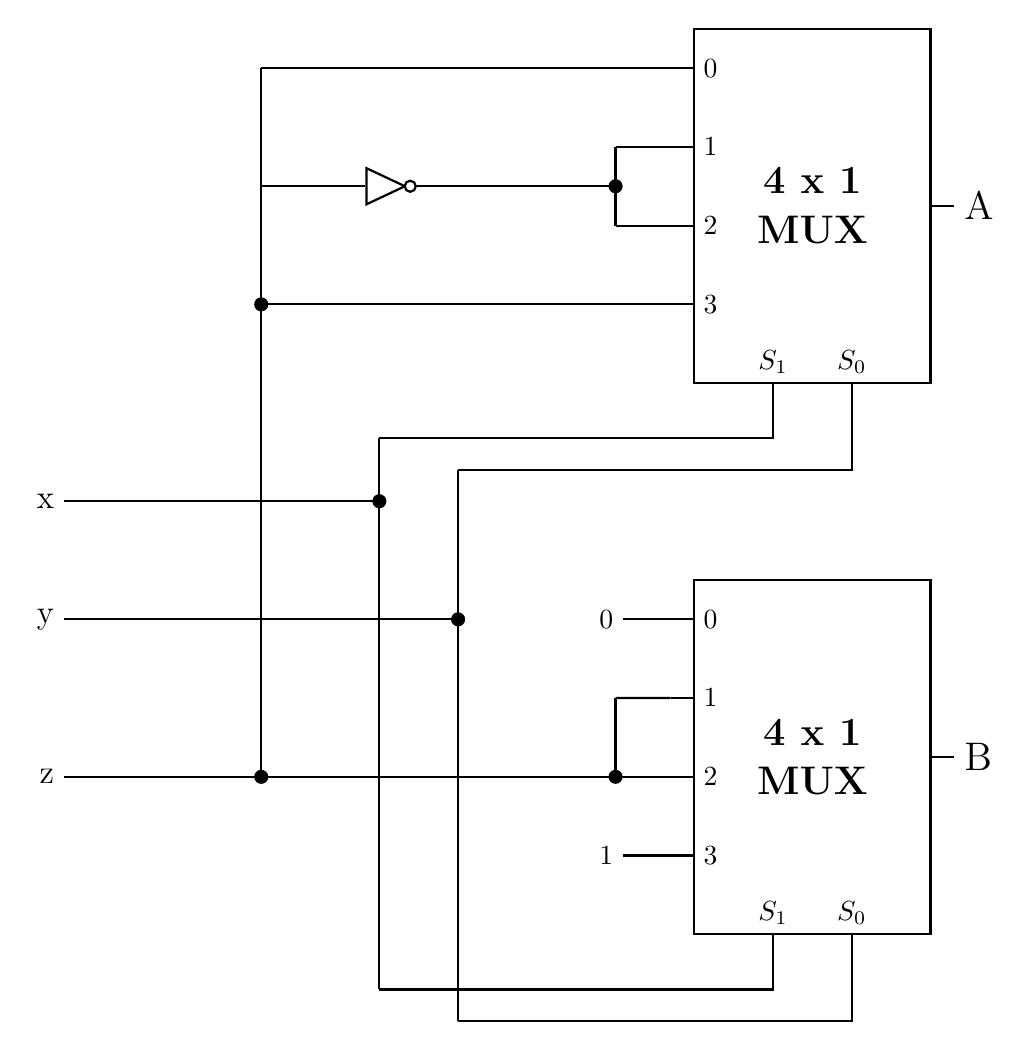
\begin{tikzpicture}[
    >=stealth,
    thick,
    dot/.style={circle, fill=black, inner sep=1.8pt, outer sep=0pt},
    every not gate US/.style={scale=1.3} % NOT gate-এর আকার ঠিক করার জন্য
]

% ==========================================
% 1. Custom 4x1 MUX Block Definition
% ==========================================
\tikzset{
    mux/.pic={
        % Main Box
        \draw (0,0) rectangle (3, 4.5);
        \node[align=center, font=\Large\bfseries] at (1.5, 2.25) {4 x 1 \\ MUX};
        
        % Data Input Pins (0, 1, 2, 3)
        \foreach \i/\y in {0/4, 1/3, 2/2, 3/1} {
            \node[anchor=west, font=\normalsize, inner sep=3pt] at (0, \y) {\i};
            \draw (0, \y) -- (-0.3, \y); % short pin line
            \coordinate (-in\i) at (-0.3, \y);
        }
        
        % Select Input Pins (S1, S0)
        \node[anchor=south, font=\normalsize, inner sep=3pt] at (1, 0) {$S_1$}; 
        \draw (1, 0) -- (1, -0.3);
        \coordinate (-s1) at (1, -0.3);
        
        \node[anchor=south, font=\normalsize, inner sep=3pt] at (2, 0) {$S_0$}; 
        \draw (2, 0) -- (2, -0.3);
        \coordinate (-s0) at (2, -0.3);
        
        % Output Pin
        \draw (3, 2.25) -- (3.3, 2.25);
        \coordinate (-out) at (3.3, 2.25);
    }
}

% ==========================================
% 2. Place MUX Components
% ==========================================
\pic (MuxA) at (8, 4.5) {mux};  % Top MUX
\pic (MuxB) at (8, -2.5) {mux}; % Bottom MUX

% Output Labels A and B
\node[right, font=\Large] at (MuxA-out) {A};
\node[right, font=\Large] at (MuxB-out) {B};

% ==========================================
% 3. Global Inputs (x, y, z)
% ==========================================
\node[left, font=\large] (varX) at (0, 3) {x};
\node[left, font=\large] (varY) at (0, 1.5) {y};
\node[left, font=\large] (varZ) at (0, -.5) {z};

% ==========================================
% 4. Routing Data Lines (Vertical Bus for x)
% ==========================================
\coordinate (Vx_bus) at (2.5, 0); % x-coordinate for the vertical x-bus

% Draw x line to the bus
\draw (varX.east) -- (4, 3) node[dot]{};

% Main vertical Vx bus line
\draw (2.5, 3) -- (2.5, 8.5); % Goes UP to Mux A
\draw (2.5, 3) -- (2.5, -0.5); % Goes DOWN to Mux B

% Connect MUX A Data Inputs to Vx bus
\draw (2.5, 8.5) -- (MuxA-in0); % Pin 0 (top bend, no dot)

\node[not gate US, draw] (not1) at (4, 7) {}; % Place NOT gate
\draw (2.5, 7)  -- (not1.input);   % Vx to NOT gate
\draw (not1.output)  -- (7,7)node[dot]{};              % NOT gate to Pin 1
\draw (7, 7.5)  -- (MuxA-in1);     % Pin 2
\draw (7,7.5) -- (7,6.5); 

\draw (7, 6.5)  -- (MuxA-in2);     % Pin 2
\draw (2.5, 5.5) node[dot]{} -- (MuxA-in3);     % Pin 3

% Connect MUX B Data Inputs
\draw (MuxA-in0 |- MuxB-in0) -- ++(-0.6, 0) node[left] {0}; % Pin 0 connected to 0
\draw (7, 0.5)  -- (MuxB-in1); 
\draw (7,0.5) -- (7,-0.5);                % Pin 1 to Vx
\draw (2.5, -0.5) node[dot]{} -- (MuxB-in2);                % Pin 2 to Vx
\draw (MuxA-in3 |- MuxB-in3) -- ++(-0.6, 0) node[left] {1}; % Pin 3 connected to 1

% ==========================================
% 5. Routing Select Lines (y, z)
% ==========================================
% Draw y and z horizontal lines to their respective vertical buses
\draw (varY.east) -- (5, 1.5) node[dot]{};
\draw (varZ.east) -- (7, -.5) node[dot]{};

% S1 Routing (connects to y)
\draw (MuxA-s1) |- (4, 3.8);   % Mux A S1 goes down and left
\draw (MuxB-s1) |- (4, -3.2);  % Mux B S1 goes down and left
\draw (4, 3.8) -- (4, -3.2);   % Vertical line combining them

% S0 Routing (connects to z)
\draw (MuxA-s0) |- (5, 3.4);   % Mux A S0 goes down and left
\draw (MuxB-s0) |- (5, -3.6);  % Mux B S0 goes down and left
\draw (5, 3.4) -- (5, -3.6);   % Vertical line combining them

\end{tikzpicture}
\end{center}
\mk{16} \yr{CSE 205 | L-2/T-1 | 2014--15}

\begin{tcolorbox}[enhanced,breakable,ansbox,colback=cB!4,colframe=cB,boxrule=0.8pt,arc=5pt,title={\textbf{Answer}},fonttitle=\bfseries\color{white},colbacktitle=cB]

\section*{1. Circuit Analysis and Multiplexer Foundation}

A $4 \times 1$ Multiplexer (MUX) routes one of its four data inputs ($I_0, I_1, I_2, I_3$) to the output based on the value of its two selection lines ($S_1, S_0$). The canonical logic equation for a $4 \times 1$ MUX is:
\begin{equation}
    Y = S_1' S_0' I_0 + S_1' S_0 I_1 + S_1 S_0' I_2 + S_1 S_0 I_3
\end{equation}

By tracing the provided logic circuit, we can determine the global inputs applied to the select lines of both MUX A and MUX B:
\begin{itemize}
    \item The Most Significant Select Bit (\textbf{$S_1$}) is connected directly to variable \textbf{$x$}.
    \item The Least Significant Select Bit (\textbf{$S_0$}) is connected directly to variable \textbf{$y$}.
\end{itemize}
Therefore, for both multiplexers, the select lines are $(S_1, S_0) = (x, y)$.

\vspace{0.2cm}
\hrule
\vspace{0.4cm}

\section*{2. Derivation of Output Function $A$ (Sum of Minterms)}

By observing the connections to the data pins of \textbf{MUX A}, we identify the following inputs from the $z$ bus:
\begin{itemize}
    \item $I_0$ is connected directly to $z \implies I_0 = z$
    \item $I_1$ is connected through a NOT gate from $z \implies I_1 = z'$
    \item $I_2$ is connected through the same NOT gate from $z \implies I_2 = z'$
    \item $I_3$ is connected directly to $z \implies I_3 = z$
\end{itemize}

Substituting these into the MUX equation gives the Boolean function for $A$:
\begin{align*}
    A(x,y,z) &= x'y'(z) + x'y(z') + xy'(z') + xy(z)
\end{align*}

Because each term contains all three variables ($x, y, z$), the expression is already in canonical Sum of Products (SOP) form. We can map each product term to its corresponding minterm index (where uncomplemented = $1$, complemented = $0$):
\begin{align*}
    x'y'z  &\implies 001 \implies m_1 \\
    x'yz'  &\implies 010 \implies m_2 \\
    xy'z'  &\implies 100 \implies m_4 \\
    xyz    &\implies 111 \implies m_7
\end{align*}

Thus, the function $A$ as a sum of minterms is:
\begin{equation}
    \textcolor{cB}{\mathbf{A(x, y, z) = \sum m(1, 2, 4, 7)}}
\end{equation}

\vspace{0.2cm}
\hrule
\vspace{0.4cm}

\section*{3. Derivation of Output Function $B$ (Product of Maxterms)}

By observing the connections to the data pins of \textbf{MUX B}, we identify:
\begin{itemize}
    \item $I_0$ is connected to Logic $0 \implies I_0 = 0$
    \item $I_1$ is connected directly to the $z$ bus $\implies I_1 = z$
    \item $I_2$ is connected directly to the $z$ bus $\implies I_2 = z$
    \item $I_3$ is connected to Logic $1 \implies I_3 = 1$
\end{itemize}

Substituting these into the MUX equation gives the Boolean function for $B$:
\begin{align*}
    B(x,y,z) &= x'y'(0) + x'y(z) + xy'(z) + xy(1) \\
    B(x,y,z) &= x'yz + xy'z + xy
\end{align*}

To find the canonical maxterms, it is easiest to first expand the standard SOP expression into canonical minterms. We expand the term $xy$ by introducing the missing variable $z$:
\begin{align*}
    B(x,y,z) &= x'yz + xy'z + xy(z + z') && \text{(Identity \& Complementarity Laws)}\\
    B(x,y,z) &= x'yz + xy'z + xyz + xyz' && \text{(Distributive Law)}
\end{align*}

Now we identify the minterm indices for $B$:
\begin{align*}
    x'yz  &\implies 011 \implies m_3 \\
    xy'z  &\implies 101 \implies m_5 \\
    xyz'  &\implies 110 \implies m_6 \\
    xyz   &\implies 111 \implies m_7
\end{align*}
So, the minterms for $B$ are $\sum m(3, 5, 6, 7)$. 

In Boolean algebra, any term that is \textit{not} a minterm is a maxterm (where the function evaluates to 0). For a 3-variable system, the universal set of indices is $0$ through $7$. The missing indices are $0, 1, 2,$ and $4$. 

Thus, the function $B$ as a product of maxterms is:
\begin{equation}
    \textcolor{cB}{\mathbf{B(x, y, z) = \prod M(0, 1, 2, 4)}}
\end{equation}

\vspace{0.2cm}
\hrule
\vspace{0.4cm}

\section*{4. Comprehensive Truth Table Verification}

The derivations can be validated by mapping the entire system to a truth table.

\begin{center}
\renewcommand{\arraystretch}{1.2}
\begin{tabular}{ccc | c c | c c}
    \toprule
    \multicolumn{3}{c|}{\textbf{Select Inputs}} & \multicolumn{2}{c|}{\textbf{MUX A}} & \multicolumn{2}{c}{\textbf{MUX B}} \\
    $x$ ($S_1$) & $y$ ($S_0$) & $z$ & \textbf{Active Input} & \textbf{Output A} & \textbf{Active Input} & \textbf{Output B} \\
    \midrule
    0 & 0 & 0 & $I_0 = z$  & \textbf{0} & $I_0 = 0$ & \textbf{0} \\
    0 & 0 & 1 & $I_0 = z$  & \textbf{1} & $I_0 = 0$ & \textbf{0} \\
    0 & 1 & 0 & $I_1 = z'$ & \textbf{1} & $I_1 = z$ & \textbf{0} \\
    0 & 1 & 1 & $I_1 = z'$ & \textbf{0} & $I_1 = z$ & \textbf{1} \\
    1 & 0 & 0 & $I_2 = z'$ & \textbf{1} & $I_2 = z$ & \textbf{0} \\
    1 & 0 & 1 & $I_2 = z'$ & \textbf{0} & $I_2 = z$ & \textbf{1} \\
    1 & 1 & 0 & $I_3 = z$  & \textbf{0} & $I_3 = 1$ & \textbf{1} \\
    1 & 1 & 1 & $I_3 = z$  & \textbf{1} & $I_3 = 1$ & \textbf{1} \\
    \bottomrule
\end{tabular}
\end{center}

\textbf{Final Verification:}
\begin{itemize}
    \item $A$ outputs $1$ at decimal rows $1, 2, 4, 7 \implies \mathbf{A = \sum m(1, 2, 4, 7)}$
    \item $B$ outputs $0$ at decimal rows $0, 1, 2, 4 \implies \mathbf{B = \prod M(0, 1, 2, 4)}$
\end{itemize}

\end{tcolorbox}

\end{enumerate}


%% ══════════════════════════════════════════════════════════════════════
%%  SECTION 3: MINIMIZATION TECHNIQUES
%% ══════════════════════════════════════════════════════════════════════
\secdivider{Minimization Techniques}{K-Maps (2/3/4/5-variable), Quine-McCluskey, Don't-Care Conditions}{cC}{green}

\markboth{S3: Minimization Techniques}{S3: Minimization Techniques}
\label{sec:S3}
\titleformat{\section}{\large\bfseries\color{cC}}{}{0em}{}[\titlerule]
\section*{S3 \quad Minimization Techniques}
\addcontentsline{toc}{section}{S3: Minimization Techniques}

%%──────────────────────────────────────────────────────────────────────
\subtopic{cC}{Prime Implicants}
\label{sub:s3-prime-implicants}

\begin{enumerate}


\item Differentiate between prime implicant and essential prime implicant of a K-Map.
\mk{7} \yr{CSE 205 | L-2/T-1 | 2023--24, 2011--12}

\begin{tcolorbox}[enhanced,breakable,ansbox,colback=cC!4,colframe=cC,boxrule=0.8pt,arc=5pt,title={\textbf{Answer}},fonttitle=\bfseries\color{white},colbacktitle=cC]

\section*{Core Definitions}

Before differentiating the two, we must define an \textbf{Implicant}: In Boolean algebra, an implicant is any valid single group of 1s (minterms) in a Karnaugh Map that can be expressed as a product term. 

\subsection*{1. Prime Implicant (PI)}
A \textbf{\textcolor{cC}{Prime Implicant}} is an implicant that is as large as possible. It represents a group of $2^n$ minterms that cannot be completely entirely encompassed by any larger valid group. 
\begin{itemize}
    \item \textbf{Rule of Thumb:} If you can double the size of the group, the current group is \textit{not} a Prime Implicant.
    \item \textbf{Hardware Meaning:} It represents a logic gate with the absolute minimum number of inputs necessary for that specific grouping.
\end{itemize}

\subsection*{2. Essential Prime Implicant (EPI)}
An \textbf{\textcolor{cC}{Essential Prime Implicant}} is a specific type of Prime Implicant that covers \textbf{at least one minterm that is not covered by any other Prime Implicant}.
\begin{itemize}
    \item \textbf{Rule of Thumb:} If removing the group leaves a minterm stranded (uncovered), that group is essential.
    \item \textbf{Hardware Meaning:} Because it is the \textit{only} way to cover certain logic conditions, an EPI \textbf{must} be included in the final minimized hardware circuit.
\end{itemize}

\vspace{0.2cm}
\hrule
\vspace{0.4cm}

\section*{Key Differences}

\begin{center}
\renewcommand{\arraystretch}{1.5}
\begin{tabular}{p{4cm} p{5cm} p{5cm}}
    \toprule
    \textbf{Feature} & \textbf{\textcolor{cC}{Prime Implicant (PI)}} & \textbf{\textcolor{cC}{Essential Prime Implicant (EPI)}} \\
    \midrule
    \textbf{Definition} & The largest possible grouping of adjacent minterms. & A PI that contains at least one unique, isolated minterm. \\
    \textbf{Necessity in Final Expression} & \textbf{Optional.} It may or may not be included in the final minimized Boolean expression. & \textbf{Mandatory.} It \textit{must} be included in the final minimized Boolean expression. \\
    \textbf{Coverage} & All its minterms might be overlapped by other PIs. & Has at least one minterm that cannot be grouped by any other PI. \\
    \textbf{Subsets} & All EPIs are PIs, but not all PIs are EPIs. & It is a strict subset of Prime Implicants. \\
    \bottomrule
\end{tabular}
\end{center}

\vspace{0.2cm}
\hrule
\vspace{0.4cm}

\section*{Illustrative Example}

Consider the 4-variable Boolean function:
\begin{equation*}
    F(A,B,C,D) = \sum m(0, 1, 4, 5, 12, 13, 14, 15)
\end{equation*}

Let us map this onto a Karnaugh Map to identify the PIs and EPIs.

\begin{center}
    \begin{karnaugh-map}[4][4][1][$CD$][$AB$]
        \minterms{0,1,4,5,12,13,14,15}
        \autoterms[0]
        
        % EPI 1: Group (0,1,4,5) -> A'C'
        \implicant{0}{5}
        
        % EPI 2: Group (12,13,15,14) -> AB
        \implicant{12}{14}
        
        % PI but NOT EPI: Group (4,5,12,13) -> BC'
        \implicant{4}{13}
    \end{karnaugh-map}
\end{center}

\subsection*{Analysis of the K-Map:}

\begin{enumerate}
    \item \textbf{Group 1 (Red/Green Border typically):} Minterms $(0, 1, 4, 5)$. 
    \begin{itemize}
        \item It is a maximally sized $2 \times 2$ square. It is a \textbf{Prime Implicant}.
        \item Notice minterms $0$ and $1$. They cannot be covered by any other valid grouping.
        \item Therefore, this is an \textbf{\textcolor{cC}{Essential Prime Implicant (EPI)}}. (Equation: $A'C'$)
    \end{itemize}
    
    \item \textbf{Group 2 (Red/Green Border typically):} Minterms $(12, 13, 14, 15)$.
    \begin{itemize}
        \item It is a maximally sized $1 \times 4$ row. It is a \textbf{Prime Implicant}.
        \item Notice minterms $14$ and $15$. They cannot be covered by any other valid grouping.
        \item Therefore, this is an \textbf{\textcolor{cC}{Essential Prime Implicant (EPI)}}. (Equation: $AB$)
    \end{itemize}
    
    \item \textbf{Group 3 (Overlapping Middle):} Minterms $(4, 5, 12, 13)$.
    \begin{itemize}
        \item It is a maximally sized $2 \times 2$ square. It is a \textbf{Prime Implicant}.
        \item However, look closely at its minterms: $4$ and $5$ are already covered by Group 1. $12$ and $13$ are already covered by Group 2.
        \item It does \textit{not} contain any unique minterm. 
        \item Therefore, this is a \textbf{\textcolor{cC}{Prime Implicant, but NOT an Essential Prime Implicant}}. It represents redundant hardware and is discarded in the final answer. (Equation: $BC'$)
    \end{itemize}
\end{enumerate}

\textbf{Final Minimized Function (Using only EPIs):}
\begin{equation}
    F_{minimized} = A'C' + AB
\end{equation}

\end{tcolorbox}

\item Find all the prime implicants for the following Boolean function and determine which are essential:
\[ F(A, B, C, D) = \Sigma\,(0, 2, 3, 5, 7, 8, 9, 10, 11, 13, 15) \]
\mk{11} \yr{CSE 205 | L-2/T-1 | 2014--15}

\begin{tcolorbox}[enhanced,breakable,ansbox,colback=cC!4,colframe=cC,boxrule=0.8pt,arc=5pt,title={\textbf{Answer}},fonttitle=\bfseries\color{white},colbacktitle=cC]

\section*{Step 1: Plotting the Karnaugh Map}

We are given the 4-variable Boolean function:
\begin{equation*}
    F(A, B, C, D) = \Sigma\,(0, 2, 3, 5, 7, 8, 9, 10, 11, 13, 15)
\end{equation*}

We plot the given minterms (1s) onto a 4-variable Karnaugh Map. Empty cells are assumed to be 0. To avoid visual clutter from overlapping groups, only the \textbf{Essential Prime Implicants} are graphically highlighted on the map below.

\begin{center}
    \begin{karnaugh-map}[4][4][1][$CD$][$AB$]
        \minterms{0,2,3,5,7,8,9,10,11,13,15}
        \autoterms[0]
        
        % Essential Prime Implicants
        \implicantcorner % Covers 0, 2, 8, 10 -> B'D'
        \implicant{5}{15} % Covers 5, 7, 13, 15 -> BD
    \end{karnaugh-map}
\end{center}

\vspace{0.2cm}
\hrule
\vspace{0.4cm}

\section*{Step 2: Identifying All Prime Implicants (PIs)}

A \textbf{Prime Implicant} is a maximally sized grouping of 1s (size $2^n$) that cannot be entirely encompassed by any larger grouping. By inspecting all possible adjacent rectangular groups on the K-map, we identify \textbf{six} distinct Prime Implicants:

\begin{itemize}
    \item \textbf{$PI_1$}: Grouping the four corners $(0, 2, 8, 10) \implies \mathbf{B'D'}$
    \item \textbf{$PI_2$}: Grouping the center-right square $(5, 7, 13, 15) \implies \mathbf{BD}$
    \item \textbf{$PI_3$}: Grouping the entire bottom row $(8, 9, 10, 11) \implies \mathbf{AB'}$
    \item \textbf{$PI_4$}: Grouping the entire third column $(3, 7, 11, 15) \implies \mathbf{CD}$
    \item \textbf{$PI_5$}: Grouping the bottom-right $2 \times 2$ square $(9, 11, 13, 15) \implies \mathbf{AD}$
    \item \textbf{$PI_6$}: Grouping the top and bottom edge cells in columns 11 and 10 $(2, 3, 10, 11) \implies \mathbf{B'C}$
\end{itemize}

\vspace{0.2cm}
\hrule
\vspace{0.4cm}

\section*{Step 3: Prime Implicant Coverage Chart}

To systematically determine which of these PIs are \textbf{essential}, we construct a Prime Implicant Chart. An Essential Prime Implicant (EPI) must cover at least one minterm that is not covered by any other PI.

\begin{center}
\renewcommand{\arraystretch}{1.3}
\begin{tabular}{ll|ccccccccccc}
    \toprule
    \textbf{PI} & \textbf{Term} & \textbf{0} & \textbf{2} & \textbf{3} & \textbf{5} & \textbf{7} & \textbf{8} & \textbf{9} & \textbf{10} & \textbf{11} & \textbf{13} & \textbf{15} \\ 
    \midrule
    $PI_1$ (EPI) & $\mathbf{B'D'}$ & \textcolor{cC}{\textbf{X}} & X & & & & X & & X & & & \\
    $PI_2$ (EPI) & $\mathbf{BD}$ & & & & \textcolor{cC}{\textbf{X}} & X & & & & & X & X \\
    $PI_3$ & $\mathbf{AB'}$ & & & & & & X & X & X & X & & \\
    $PI_4$ & $\mathbf{CD}$ & & & X & & X & & & & X & & X \\
    $PI_5$ & $\mathbf{AD}$ & & & & & & & X & & X & X & X \\
    $PI_6$ & $\mathbf{B'C}$ & & X & X & & & & & X & X & & \\
    \bottomrule
\end{tabular}
\end{center}

\vspace{0.2cm}
\hrule
\vspace{0.4cm}

\section*{Step 4: Conclusion}

By examining the columns of the Prime Implicant chart, we look for columns that contain only a single 'X'. These identify minterms that are uniquely covered by only one logic block.
\begin{itemize}
    \item \textbf{Minterm 0} is uniquely covered by $PI_1$ ($B'D'$).
    \item \textbf{Minterm 5} is uniquely covered by $PI_2$ ($BD$).
\end{itemize}
All other minterms are covered by overlapping groups (two or more PIs). Therefore, $PI_1$ and $PI_2$ are strictly essential to the final minimized circuit.

\vspace{0.3cm}
\textbf{Final Results:}
\begin{align*}
    \text{\textbf{All Prime Implicants:}} \quad & \textcolor{cC}{\mathbf{B'D',\; BD,\; AB',\; CD,\; AD,\; B'C}} \\
    \text{\textbf{Essential Prime Implicants:}} \quad & \textcolor{cC}{\mathbf{B'D',\; BD}}
\end{align*}

\end{tcolorbox}

\end{enumerate}

%%──────────────────────────────────────────────────────────────────────
\subtopic{cC}{Karnaugh Map}
\label{sub:s3-kmap}

\begin{enumerate}

\item Using K-Map, minimize $f(v,w,x,y,z) = \Sigma\,(2,7,8,15,22,23,25,29) + d(6,9,13,18,24,31)$. Find the Prime Implicants and Essential Prime Implicants, and the Minimal Sums. Write down the responsible minterm for each Essential Prime Implicant.
\mk{15} \yr{CSE 205 | L-2/T-1 | 2020--21}

\begin{tcolorbox}[enhanced,breakable,ansbox,colback=cC!4,colframe=cC,boxrule=0.8pt,arc=5pt,title={\textbf{Answer}},fonttitle=\bfseries\color{white},colbacktitle=cC]

\section*{1. 5-Variable Karnaugh Map Setup}

For a 5-variable function $f(v,w,x,y,z)$, we construct two 4-variable K-maps. The first map corresponds to $v = 0$ (minterms $0$ to $15$) and the second map corresponds to $v = 1$ (minterms $16$ to $31$).

Given:
\begin{align*}
    \text{Minterms (1s)} &: \Sigma\,(2, 7, 8, 15, 22, 23, 25, 29) \\
    \text{Don't Cares (Xs)} &: d(6, 9, 13, 18, 24, 31)
\end{align*}

We distribute these into the respective maps. For the $v=1$ map, the physical cell locations correspond to the given minterm/don't care index minus $16$.

To maintain visual clarity, the K-maps below explicitly show the groupings for \textbf{one} of the valid Minimal Sums ($MS_1$). All Prime Implicants will be listed systematically in the next section.

\begin{center}
\begin{tabular}{c c}
    \textbf{Map for $v=0$} & \textbf{Map for $v=1$} \\
    \begin{karnaugh-map}[4][4][1][$yz$][$wx$]
        % Minterms for v=0: 2, 7, 8, 15
        \minterms{2,7,8,15}
        % Don't cares for v=0: 6, 9, 13
        \indeterminants{6,9,13}
        \autoterms[0]
        
        % Groupings for MS1
        \implicant{2}{6}   % w'yz'
        \implicant{8}{9}   % wx'y'
        \implicant{7}{15}  % xyz
        \implicant{13}{9}  % wy'z
    \end{karnaugh-map}
    &
    \begin{karnaugh-map}[4][4][1][$yz$][$wx$]
        % Minterms for v=1 (index - 16): 22->6, 23->7, 25->9, 29->13
        \minterms{6,7,9,13}
        % Don't cares for v=1 (index - 16): 18->2, 24->8, 31->15
        \indeterminants{2,8,15}
        \autoterms[0]
        
        % Groupings for MS1
        \implicant{2}{6}   % w'yz'
        \implicant{8}{9}   % wx'y'
        \implicant{7}{15}  % xyz
        \implicant{13}{9}  % wy'z
    \end{karnaugh-map}
\end{tabular}
\end{center}

\vspace{0.2cm}
\hrule
\vspace{0.4cm}

\section*{2. Identification of Prime Implicants (PIs)}

By systematically grouping the maximum number of adjacent $1$s and $X$s (in sizes of $2^n$), we identify the following \textbf{six} Prime Implicants. Notice that these groups span symmetrically across both the $v=0$ and $v=1$ maps, thereby eliminating the variable $v$.

\begin{itemize}
    \item \textbf{$PI_1$:} Grouping $(2, 6, 18, 22) \implies \textcolor{cC}{\mathbf{w'yz'}}$
    \item \textbf{$PI_2$:} Grouping $(8, 9, 24, 25) \implies \textcolor{cC}{\mathbf{wx'y'}}$
    \item \textbf{$PI_3$:} Grouping $(7, 15, 23, 31) \implies \textcolor{cC}{\mathbf{xyz}}$
    \item \textbf{$PI_4$:} Grouping $(9, 13, 25, 29) \implies \textcolor{cC}{\mathbf{wy'z}}$
    \item \textbf{$PI_5$:} Grouping $(13, 15, 29, 31) \implies \textcolor{cC}{\mathbf{wxz}}$
    \item \textbf{$PI_6$:} Grouping $(6, 7, 22, 23) \implies \textcolor{cC}{\mathbf{w'xy}}$
\end{itemize}

\vspace{0.2cm}
\hrule
\vspace{0.4cm}

\section*{3. Essential Prime Implicants (EPIs) and Coverage}

To determine the Essential Prime Implicants, we construct a PI Coverage Chart. We only list the true minterms (excluding don't cares) because don't cares do not strictly need to be covered.

\begin{center}
\renewcommand{\arraystretch}{1.3}
\begin{tabular}{cl|cccccccc}
    \toprule
    \textbf{PI} & \textbf{Term} & \textbf{2} & \textbf{7} & \textbf{8} & \textbf{15} & \textbf{22} & \textbf{23} & \textbf{25} & \textbf{29} \\ 
    \midrule
    $PI_1$ & $\mathbf{w'yz'}$ & \textcolor{cC}{\textbf{X}} & & & & X & & & \\
    $PI_2$ & $\mathbf{wx'y'}$ & & & \textcolor{cC}{\textbf{X}} & & & & X & \\
    $PI_3$ & $\mathbf{xyz}$ & & X & & X & & X & & \\
    $PI_4$ & $\mathbf{wy'z}$ & & & & & & & X & X \\
    $PI_5$ & $\mathbf{wxz}$ & & & & X & & & & X \\
    $PI_6$ & $\mathbf{w'xy}$ & & X & & & X & X & & \\
    \bottomrule
\end{tabular}
\end{center}

By scanning the columns for single 'X' marks, we find the EPIs and their responsible minterms:
\begin{itemize}
    \item \textbf{Minterm 2} is covered \textit{only} by $PI_1$. Thus, \textcolor{cC}{$\mathbf{w'yz'}$} is an EPI.
    \item \textbf{Minterm 8} is covered \textit{only} by $PI_2$. Thus, \textcolor{cC}{$\mathbf{wx'y'}$} is an EPI.
\end{itemize}

\textbf{Summary of EPIs \& Responsible Minterms:}
\begin{align*}
    \text{EPI: } \mathbf{w'yz'} \quad &\longrightarrow \quad \text{Responsible minterm: } \mathbf{m_2} \\
    \text{EPI: } \mathbf{wx'y'} \quad &\longrightarrow \quad \text{Responsible minterm: } \mathbf{m_8}
\end{align*}

\vspace{0.2cm}
\hrule
\vspace{0.4cm}

\section*{4. Minimal Sums}

Selecting the two EPIs ($PI_1$ and $PI_2$) automatically covers minterms $2, 8, 22,$ and $25$. 
The minterms remaining to be covered are: \textbf{$\{7, 15, 23, 29\}$}.

We must cover these remaining minterms using the fewest possible remaining PIs. Since all PIs are 3-literal terms, cost is identical across choices. Let us evaluate combinations of 2 additional PIs that satisfy the remaining cover:
\begin{enumerate}
    \item Selecting $PI_3$ covers $\{7, 15, 23\}$. We still need $29$, which is covered by $PI_4$. $\implies \{PI_3, PI_4\}$
    \item Selecting $PI_5$ covers $\{15, 29\}$. We still need $\{7, 23\}$, which is covered by $PI_6$. $\implies \{PI_5, PI_6\}$
    \item Selecting $PI_3$ covers $\{7, 15, 23\}$. Selecting $PI_5$ covers $\{15, 29\}$. Together they cover all remaining. $\implies \{PI_3, PI_5\}$
\end{enumerate}

Therefore, there are exactly \textbf{three} valid Minimal Sums for this function:
\begin{align*}
    \text{\textbf{Minimal Sum 1:}} \quad f &= \textcolor{cC}{\mathbf{w'yz' + wx'y' + xyz + wy'z}} \\
    \text{\textbf{Minimal Sum 2:}} \quad f &= \textcolor{cC}{\mathbf{w'yz' + wx'y' + w'xy + wxz}} \\
    \text{\textbf{Minimal Sum 3:}} \quad f &= \textcolor{cC}{\mathbf{w'yz' + wx'y' + xyz + wxz}}
\end{align*}

\end{tcolorbox}

\item Convert the following Boolean function from sum-of-products form to a simplified product-of-sums form, then draw a logic circuit for the POS form:
\[ F(w,x,y,z) = \Sigma\,(0,1,2,5,7,11,13) \]
\mk{20} \yr{CSE 205 | L-2/T-1 | 2019--20}

\begin{tcolorbox}[enhanced,breakable,ansbox,colback=cC!4,colframe=cC,boxrule=0.8pt,arc=5pt,title={\textbf{Answer}},fonttitle=\bfseries\color{white},colbacktitle=cC]

\textbf{Step 1: Identify the Maxterms} \\
The Boolean function is given in canonical Sum-of-Products (SOP) form with minterms:
\[ F(w,x,y,z) = \Sigma\,(0,1,2,5,7,11,13) \]
For a 4-variable function, the total possible minterms range from 0 to 15. The minterms that are \textit{not} present in $F$ correspond to the maxterms (zeros) of the function.
\[ F(w,x,y,z) = \Pi\,(3,4,6,8,9,10,12,14,15) \]

\vspace{0.3cm}
\textbf{Step 2: Karnaugh Map for Product-of-Sums (POS) Minimization} \\
To find the simplified POS expression, we map the zeros (maxterms) of $F$ on a Karnaugh map. Grouping the zeros directly yields the minimal sum terms. 

\begin{center}
\begin{karnaugh-map}[4][4][1][$yz$][$wx$]
    % Placing 0s for maxterms
    \maxterms{3,4,6,8,9,10,12,14,15}
    % Filling the rest with 1s (the given minterms)
    \minterms{0,1,2,5,7,11,13}
    
    % Group 1: isolated zero at 3
    \implicant{3}{3}
    % Group 2: pair of zeros at 8, 9
    \implicant{8}{9}
    % Group 3: pair of zeros at 14, 15
    \implicant{15}{14}
    % Group 4: quad of zeros at 4, 6, 12, 14 (edges)
    \implicantedge{4}{12}{6}{14}
    % Group 5: quad of zeros at 8, 10, 12, 14 (bottom rows edges)
    \implicantedge{12}{8}{14}{10}
\end{karnaugh-map}
\end{center}

\textbf{Step 3: Deriving the Sum Terms} \\
From the groups of zeros, we extract the corresponding sum terms. Remember that for zeros (POS), an input value of $0$ is represented by the uncomplemented variable, and an input value of $1$ is represented by the complemented variable.

\begin{itemize}
    \item \textbf{Group 1 (Single 0 at $m_3$):} Fixed $w=0, x=0, y=1, z=1 \implies \mathbf{(w + x + y' + z')}$
    \item \textbf{Group 2 (Pair at 14, 15):} Fixed $w=1, x=1, y=1 \implies \mathbf{(w' + x' + y')}$
    \item \textbf{Group 3 (Pair at 8, 9):} Fixed $w=1, x=0, y=0 \implies \mathbf{(w' + x + y)}$
    \item \textbf{Group 4 (Quad at 4, 6, 12, 14):} Fixed $x=1, z=0 \implies \mathbf{(x' + z)}$
    \item \textbf{Group 5 (Quad at 8, 10, 12, 14):} Fixed $w=1, z=0 \implies \mathbf{(w' + z)}$
\end{itemize}

\textit{Algebraic Verification (De Morgan's Law):}
If we grouped the same cells as 1s for the complement function $F'$, we would get $F' = w'x'yz + wxy + wx'y' + xz' + wz'$. Taking the complement of both sides and applying De Morgan's Law gives:
\begin{align*}
    F &= (F')' \\
    &= (w'x'yz + wxy + wx'y' + xz' + wz')' \\
    &= (w'x'yz)' \cdot (wxy)' \cdot (wx'y')' \cdot (xz')' \cdot (wz')' \quad &&\text{(De Morgan's Law: } (A+B)' = A'B'\text{)} \\
    &= \textcolor{cC}{\mathbf{(w + x + y' + z')(w' + x' + y')(w' + x + y)(x' + z)(w' + z)}} \quad &&\text{(De Morgan's Law: } (AB)' = A'+B'\text{)}
\end{align*}

\vspace{0.3cm}
\textbf{Step 4: Logic Circuit Diagram for POS Form} \\
The POS function is implemented using a 2-level OR-AND logic structure. 

\begin{center}
\begin{circuitikz}[scale=0.95, transform shape, thick]
    % Final AND gate (Level 2)
    \node[and port, number inputs=5] (AND) at (10, -4) {};
    \draw (AND.out) -- ++(0.5,0) node[right] {$F$};

    % OR gates (Level 1)
    \node[or port, number inputs=4] (OR1) at (4, -0.8) {};
    \node[or port, number inputs=3] (OR2) at (4, -2.4) {};
    \node[or port, number inputs=3] (OR3) at (4, -4) {};
    \node[or port] (OR4) at (4, -5.6) {};
    \node[or port] (OR5) at (4, -7.2) {};

    % Clean manhattan routing from ORs to AND
    \draw (OR1.out) -- ++(2.5,0) |- (AND.in 1);
    \draw (OR2.out) -- ++(1.5,0) |- (AND.in 2);
    \draw (OR3.out) -- (AND.in 3); % Straight line naturally aligns
    \draw (OR4.out) -- ++(1.5,0) |- (AND.in 4);
    \draw (OR5.out) -- ++(2.5,0) |- (AND.in 5);

    % Inputs to OR1 (w + x + y' + z')
    \draw (OR1.in 1) -- ++(-0.6,0) node[left] {$w$};
    \draw (OR1.in 2) -- ++(-0.6,0) node[left] {$x$};
    \draw (OR1.in 3) -- ++(-0.6,0) node[left] {$y'$};
    \draw (OR1.in 4) -- ++(-0.6,0) node[left] {$z'$};

    % Inputs to OR2 (w' + x' + y')
    \draw (OR2.in 1) -- ++(-0.6,0) node[left] {$w'$};
    \draw (OR2.in 2) -- ++(-0.6,0) node[left] {$x'$};
    \draw (OR2.in 3) -- ++(-0.6,0) node[left] {$y'$};

    % Inputs to OR3 (w' + x + y)
    \draw (OR3.in 1) -- ++(-0.6,0) node[left] {$w'$};
    \draw (OR3.in 2) -- ++(-0.6,0) node[left] {$x$};
    \draw (OR3.in 3) -- ++(-0.6,0) node[left] {$y$};

    % Inputs to OR4 (x' + z)
    \draw (OR4.in 1) -- ++(-0.6,0) node[left] {$x'$};
    \draw (OR4.in 2) -- ++(-0.6,0) node[left] {$z$};

    % Inputs to OR5 (w' + z)
    \draw (OR5.in 1) -- ++(-0.6,0) node[left] {$w'$};
    \draw (OR5.in 2) -- ++(-0.6,0) node[left] {$z$};
\end{circuitikz}
\end{center}

\end{tcolorbox}

\item Using K-Map, minimize $f(w,x,y,z) = \Sigma\,(1,2,3,7,10,12,14) + d(0,6,8,13)$. Find the Prime Implicants and Essential Prime Implicants. Write down the responsible minterm for each Essential Prime Implicant.
\mk{12} \yr{CSE 205 | L-2/T-1 | 2018--19}

\begin{tcolorbox}[enhanced,breakable,ansbox,colback=cC!4,colframe=cC,boxrule=0.8pt,arc=5pt,title={\textbf{Answer}},fonttitle=\bfseries\color{white},colbacktitle=cC]

\textbf{1. Karnaugh Map Construction} \\
The Boolean function is given as $f(w,x,y,z) = \Sigma\,(1,2,3,7,10,12,14) + d(0,6,8,13)$. We map the minterms as '1', the don't cares as 'd', and the remaining cells as '0'. 

\begin{center}
\begin{karnaugh-map}[4][4][1][$yz$][$wx$]
    % Placing minterms and don't cares
    \minterms{1,2,3,7,10,12,14}
    \indeterminants{0,6,8,13}
    \autoterms[0]
    
    % Highlighting the groupings that form the minimal cover
    \implicant{0}{2}          % Quad: w'x'
    \implicant{3}{6}          % Quad: w'y
    \implicantedge{12}{8}{14}{10} % Quad: wz' (wrapping top/bottom rows)
\end{karnaugh-map}
\end{center}

\vspace{0.3cm}
\textbf{2. Identifying Prime Implicants (PIs)} \\
A Prime Implicant is a maximal grouping of 1s and don't cares (i.e., a group that cannot be entirely consumed by a larger valid group). By analyzing the K-Map, we extract all possible maximal groupings:

\begin{center}
\begin{tabular}{llc}
    \toprule
    \textbf{Prime Implicant} & \textbf{Cells Covered} & \textbf{Minterms Covered (excluding 'd')} \\
    \midrule
    $w'x'$ & $0, 1, 3, 2$ & $m_1, m_2, m_3$ \\
    $w'y$ & $3, 2, 7, 6$ & $m_2, m_3, m_7$ \\
    $x'z'$ & $0, 2, 8, 10$ & $m_2, m_{10}$ \\
    $yz'$ & $2, 6, 14, 10$ & $m_2, m_{10}, m_{14}$ \\
    $wz'$ & $12, 14, 8, 10$ & $m_{10}, m_{12}, m_{14}$ \\
    $wxy'$ & $12, 13$ & $m_{12}$ \\
    \bottomrule
\end{tabular}
\end{center}

\vspace{0.3cm}
\textbf{3. Essential Prime Implicants (EPIs)} \\
An Essential Prime Implicant is a PI that covers at least one minterm (1) that is \textit{not} covered by any other Prime Implicant. This exclusively covered minterm is known as the \textit{responsible minterm} or \textit{distinguished minterm}.

By cross-referencing our PIs:
\begin{itemize}
    \item Minterm $m_1$ is covered \textbf{only} by the PI $w'x'$.
    \item Minterm $m_7$ is covered \textbf{only} by the PI $w'y$.
    \item All other minterms ($m_2, m_{10}, m_{12}, m_{14}$) are covered by at least two different PIs.
\end{itemize}

\begin{center}
\begin{tabular}{lc}
    \toprule
    \textbf{Essential Prime Implicant} & \textbf{Responsible Minterm} \\
    \midrule
    \textcolor{cC}{$\mathbf{w'x'}$} & $m_1$ \\
    \textcolor{cC}{$\mathbf{w'y}$} & $m_7$ \\
    \bottomrule
\end{tabular}
\end{center}

\vspace{0.3cm}
\textbf{4. Minimal Sum-of-Products (SOP) Expression} \\
To find the final minimized expression, we must first include all Essential Prime Implicants, which cover minterms $m_1, m_2, m_3,$ and $m_7$. 

The remaining uncovered minterms are $m_{10}, m_{12},$ and $m_{14}$. Looking at our list of available PIs, the single implicant $wz'$ perfectly covers all three of these remaining minterms simultaneously, making it the most optimal choice to complete the function.

\begin{align*}
    f(w,x,y,z) &= \text{EPIs} + \text{Remaining Minimal Cover} \\
    f(w,x,y,z) &= \textcolor{cC}{\mathbf{w'x' + w'y + wz'}}
\end{align*}

\end{tcolorbox}

\item Using K-Map, minimize $f(w,x,y,z) = \mathrm{SOP}(1,2,4,7,9,10,12,14) + d(0,6,8,13)$. Find the Prime Implicants and Essential Prime Implicants. Write down the responsible minterm for each Essential Prime Implicant.
\mk{12} \yr{CSE 205 | L-2/T-1 | 2017--18}

\begin{tcolorbox}[enhanced,breakable,ansbox,colback=cC!4,colframe=cC,boxrule=0.8pt,arc=5pt,title={\textbf{Answer}},fonttitle=\bfseries\color{white},colbacktitle=cC]

\textbf{1. Karnaugh Map Construction} \\
The Boolean function is given as $f(w,x,y,z) = \mathrm{SOP}(1,2,4,7,9,10,12,14) + d(0,6,8,13)$. We plot the minterms as '1', the don't cares as 'd', and leave the remaining cells as '0'. 

\begin{center}
\begin{karnaugh-map}[4][4][1][$yz$][$wx$]
    % Placing minterms and don't cares
    \minterms{1,2,4,7,9,10,12,14}
    \indeterminants{0,6,8,13}
    \autoterms[0]
    
    % Highlighting the groupings that form the minimal cover
    \implicantedge{0}{1}{8}{9}      % Quad: x'y' (wrapping top/bottom rows, left side)
    \implicant{7}{6}                % Pair: w'xy
    \implicantedge{4}{12}{6}{14}    % Quad: xz' (wrapping left/right edges, middle rows)
    \implicant{2}{10}               % Quad: yz' (entire rightmost column)
\end{karnaugh-map}
\end{center}

\vspace{0.3cm}
\textbf{2. Identifying Prime Implicants (PIs)} \\
A Prime Implicant is a maximal grouping of 1s and don't cares (i.e., a group that cannot be entirely consumed by a larger valid group). By thoroughly analyzing the K-Map, we extract all possible maximal groupings:

\begin{center}
\begin{tabular}{llc}
    \toprule
    \textbf{Prime Implicant} & \textbf{Cells Covered} & \textbf{Minterms Covered (excluding 'd')} \\
    \midrule
    $x'y'$ & $0, 1, 8, 9$ & $m_1, m_9$ \\
    $wy'$  & $8, 9, 12, 13$ & $m_9, m_{12}$ \\
    $y'z'$ & $0, 4, 8, 12$ & $m_4, m_{12}$ \\
    $xz'$  & $4, 6, 12, 14$ & $m_4, m_{12}, m_{14}$ \\
    $yz'$  & $2, 6, 10, 14$ & $m_2, m_{10}, m_{14}$ \\
    $x'z'$ & $0, 2, 8, 10$ & $m_2, m_{10}$ \\
    $w'xy$ & $6, 7$ & $m_7$ \\
    \bottomrule
\end{tabular}
\end{center}

\vspace{0.3cm}
\textbf{3. Essential Prime Implicants (EPIs)} \\
An Essential Prime Implicant is a PI that covers at least one minterm (1) that is \textit{not} covered by any other Prime Implicant. This exclusively covered minterm is known as the \textit{responsible minterm}.

By cross-referencing our PIs with the minterms they cover:
\begin{itemize}
    \item Minterm $m_1$ is covered \textbf{only} by the PI $x'y'$.
    \item Minterm $m_7$ is covered \textbf{only} by the PI $w'xy$.
    \item All other minterms ($m_2, m_4, m_9, m_{10}, m_{12}, m_{14}$) are covered by at least two different PIs.
\end{itemize}

\begin{center}
\begin{tabular}{lc}
    \toprule
    \textbf{Essential Prime Implicant} & \textbf{Responsible Minterm} \\
    \midrule
    \textcolor{cC}{$\mathbf{x'y'}$} & $m_1$ \\
    \textcolor{cC}{$\mathbf{w'xy}$} & $m_7$ \\
    \bottomrule
\end{tabular}
\end{center}

\vspace{0.3cm}
\textbf{4. Minimal Sum-of-Products (SOP) Expression} \\
To find the final minimized expression, we must first include all Essential Prime Implicants, which cover minterms $m_1, m_7$, and $m_9$ (since $m_9$ is absorbed by $x'y'$). 

The remaining uncovered minterms are $m_2, m_4, m_{10}, m_{12},$ and $m_{14}$. 
Looking at our list of available PIs, we want to select the minimum number of implicants to cover these five minterms:
\begin{itemize}
    \item Selecting $yz'$ covers $m_2, m_{10},$ and $m_{14}$.
    \item Selecting $xz'$ covers $m_4, m_{12},$ and $m_{14}$.
\end{itemize}
These two PIs together perfectly cover all of the remaining minterms. Adding them to our EPIs yields the optimal and complete sum-of-products equation.

\begin{align*}
    f(w,x,y,z) &= \text{EPIs} + \text{Remaining Minimal Cover} \\
    f(w,x,y,z) &= \textcolor{cC}{\mathbf{x'y' + w'xy + xz' + yz'}}
\end{align*}

\end{tcolorbox}

\item Using K-map, solve $f(x_1,x_2,x_3,x_4,x_5) = \Sigma\,(0,2,4,5,6,7,8,10,14,17,18,21,29,31) + d\Sigma\,(11,20,22)$. Find the essential prime implicants. (Show the reduction steps.)
\mk{15} \yr{CSE 205 | L-2/T-1 | 2016--17}

\begin{tcolorbox}[enhanced,breakable,ansbox,colback=cC!4,colframe=cC,boxrule=0.8pt,arc=5pt,title={\textbf{Answer}},fonttitle=\bfseries\color{white},colbacktitle=cC]

\textbf{1. Problem Statement \& Setup}

We are given a 5-variable Boolean function defined by its minterms (Sum of Products) and don't care conditions:
\begin{align*}
    f(x_1,x_2,x_3,x_4,x_5) &= \Sigma\,(0,2,4,5,6,7,8,10,14,17,18,21,29,31) + d\Sigma\,(11,20,22)
\end{align*}
To minimize this function, we construct a 5-variable Karnaugh Map. A 5-variable K-map is visually represented as two adjacent 4-variable K-maps. The left map corresponds to $x_1 = 0$ and the right map corresponds to $x_1 = 1$. The cells represent the remaining variables $x_2, x_3, x_4, x_5$.

\vspace{1em}
\textbf{2. Karnaugh Map Construction}

We populate the map with $1$ for the minterms, $d$ for the don't care conditions, and $0$ for the remaining cells. Groupings are made to cover all $1$s using the largest possible combinations (sizes of $2^n$), utilizing don't cares ($d$) only when they help to enlarge a group.

\begin{center}
\begin{karnaugh-map}[4][4][2][$x_4x_5$][$x_2x_3$][$x_1$]
    % Plotting minterms
    \minterms{0,2,4,5,6,7,8,10,14,17,18,21,29,31}
    % Setting remaining empty cells to 0
    \autoterms[0]
    % Plotting don't cares
    \indeterminants{11,20,22}
    
    % Groupings for x1 = 0 map
    \implicantcorner{0}{10} % Group 1: 0, 2, 8, 10
    \implicant{4}{6}        % Group 2: 4, 5, 7, 6
    \implicant{2}{10}       % Group 3: 2, 6, 14, 10
    
    % Groupings for x1 = 1 map
    \implicant{17}{21}      % Group 5: 17, 21
    \implicant{29}{31}      % Group 6: 29, 31
    
    % Cross-map Groupings (spanning both x1=0 and x1=1)
    \implicant{2}{22}       % Group 4: 2, 6, 18, 22
\end{karnaugh-map}
\end{center}

\vspace{1em}
\textbf{3. Algebraic Foundation of Reduction Steps}

Visual grouping on a K-map is mathematically grounded in the \textbf{Adjacency Theorem} ($XY + XY' = X$). When we group cells, we systematically eliminate variables that exist in both their true and complemented forms. Let us explicitly demonstrate the Boolean theorems applied during these reductions:

\textit{Example 1: A Pair (Group 5 - Minterms 17 and 21)}
\begin{align*}
    m_{17} + m_{21} &= x_1 x_2' x_3' x_4' x_5 + x_1 x_2' x_3 x_4' x_5 \\
    &= x_1 x_2' x_4' x_5 (x_3' + x_3) && \text{(Distributive Law)} \\
    &= x_1 x_2' x_4' x_5 (1) && \text{(Complementarity Law: $A + A' = 1$)} \\
    &= x_1 x_2' x_4' x_5 && \text{(Identity Law: $A \cdot 1 = A$)}
\end{align*}

\textit{Example 2: A Quad (Group 2 - Minterms 4, 5, 6, 7)}
\begin{align*}
    m_4 + m_5 + m_6 + m_7 &= x_1'x_2'x_3x_4'x_5' + x_1'x_2'x_3x_4'x_5 + x_1'x_2'x_3x_4x_5' + x_1'x_2'x_3x_4x_5 \\
    &= x_1'x_2'x_3x_4'(x_5' + x_5) + x_1'x_2'x_3x_4(x_5' + x_5) && \text{(Distributive Law)} \\
    &= x_1'x_2'x_3x_4'(1) + x_1'x_2'x_3x_4(1) && \text{(Complementarity Law)} \\
    &= x_1'x_2'x_3(x_4' + x_4) && \text{(Distributive \& Identity Laws)} \\
    &= x_1'x_2'x_3 && \text{(Complementarity \& Identity Laws)}
\end{align*}

\vspace{1em}
\textbf{4. Identification of Essential Prime Implicants (EPIs)}

A Prime Implicant (PI) becomes an \textbf{Essential Prime Implicant} if it is the \textit{only} possible group that covers a specific minterm. To find the minimal Sum of Products (SOP), we must include all EPIs.

Let us evaluate the mapped groups to find the essential ones:

\begin{center}
\renewcommand{\arraystretch}{1.3}
\begin{tabular}{@{}lllc@{}}
\toprule
\textbf{Group Identifier} & \textbf{Simplified Term} & \textbf{Minterms Covered} & \textbf{Distinguishing Minterm} \\
\midrule
$G_1$ (4-corners of $x_1=0$) & $x_1' x_3' x_5'$ & $0, 2, 8, 10$ & \textcolor{cC}{\textbf{8}} \\
$G_2$ (Full row in $x_1=0$) & $x_1' x_2' x_3$ & $4, 5, 6, 7$ & \textcolor{cC}{\textbf{7}} \\
$G_3$ (Full column in $x_1=0$) & $x_1' x_4 x_5'$ & $2, 6, 10, 14$ & \textcolor{cC}{\textbf{14}} \\
$G_4$ (Spans both maps) & $x_2' x_4 x_5'$ & $2, 6, 18, 22$ (d) & \textcolor{cC}{\textbf{18}} \\
$G_5$ (Pair in $x_1=1$) & $x_1 x_2' x_4' x_5$ & $17, 21$ & \textcolor{cC}{\textbf{17}} \\
$G_6$ (Pair in $x_1=1$) & $x_1 x_2 x_3 x_5$ & $29, 31$ & \textcolor{cC}{\textbf{31}} \\
\bottomrule
\end{tabular}
\end{center}

Every group listed above contains at least one minterm (highlighted in the final column) that cannot be covered by any other valid grouping. Therefore, \textbf{all six of these groups are Essential Prime Implicants}. 

\vspace{1em}
\textbf{5. Final Minimal SOP Expression}

We must now verify if any valid $1$s remain uncovered by the established EPIs. 
The set of minterms covered by the union of $G_1$ through $G_6$ is:
$$ \{0, 2, 8, 10\} \cup \{4, 5, 6, 7\} \cup \{2, 6, 10, 14\} \cup \{2, 6, 18\} \cup \{17, 21\} \cup \{29, 31\} $$
$$ = \{0, 2, 4, 5, 6, 7, 8, 10, 14, 17, 18, 21, 29, 31\} $$
This perfectly matches our original function's minterm list. Because there are no remaining uncovered minterms, the minimal expression is simply the logical OR (sum) of all the Essential Prime Implicants.

\begin{center}
\fcolorbox{cC}{cC!10}{
\parbox{0.9\linewidth}{
\vspace{0.2em}
\textbf{Minimal SOP Expression:}
\begin{align*}
    f(x_1,x_2,x_3,x_4,x_5) = \;& \textcolor{cC}{\mathbf{x_1' x_3' x_5'}} + \textcolor{cC}{\mathbf{x_1' x_2' x_3}} + \textcolor{cC}{\mathbf{x_1' x_4 x_5'}} \\ 
    &+ \textcolor{cC}{\mathbf{x_2' x_4 x_5'}} + \textcolor{cC}{\mathbf{x_1 x_2' x_4' x_5}} + \textcolor{cC}{\mathbf{x_1 x_2 x_3 x_5}}
\end{align*}
}
}
\end{center}

\end{tcolorbox}

\item Using K-maps, find the simplified product of sums form of the following Boolean function:
\[ f(w, x, y, z) = \Sigma\,(1, 5, 8, 12, 14, 15), \quad \text{don't-care minterms: } d = \Sigma\,(3, 11) \]
\mk{10} \yr{CSE 205 | L-2/T-1 | 2015--16}

\begin{tcolorbox}[enhanced,breakable,ansbox,colback=cC!4,colframe=cC,boxrule=0.8pt,arc=5pt,title={\textbf{Answer}},fonttitle=\bfseries\color{white},colbacktitle=cC]

\textbf{1. Problem Statement \& Maxterm Identification}

We are tasked with finding the simplified \textbf{Product of Sums (POS)} form for the 4-variable Boolean function:
\[ f(w, x, y, z) = \Sigma\,(1, 5, 8, 12, 14, 15), \quad d = \Sigma\,(3, 11) \]

To find the POS form, we must group the \textbf{Maxterms} (the $0$s) in the Karnaugh map. The total number of combinations for 4 variables is $16$ (from $0$ to $15$). 
The Maxterms are the missing combinations not covered by the given minterms ($1$s) or don't-care conditions ($d$s):
\begin{align*}
    \text{Total Set} &= \{0, 1, 2, 3, 4, 5, 6, 7, 8, 9, 10, 11, 12, 13, 14, 15\} \\
    \text{Minterms } (1\text{s}) &= \{1, 5, 8, 12, 14, 15\} \\
    \text{Don't-cares } (d\text{s}) &= \{3, 11\} \\
    \text{Maxterms } (\Pi) &= \text{Total Set} - (\text{Minterms} \cup \text{Don't-cares}) \\
    \Pi &= \{0, 2, 4, 6, 7, 9, 10, 13\}
\end{align*}

Thus, the function in standard POS form (with don't-cares) is:
\[ f(w,x,y,z) = \Pi\,(0, 2, 4, 6, 7, 9, 10, 13) \cdot d\,(3, 11) \]

\vspace{1em}
\textbf{2. Karnaugh Map Construction}

We populate the K-map by placing $0$s at the Maxterm locations, $d$s at the don't-care locations, and $1$s elsewhere. To simplify for POS, we group the $0$s. We can use the $d$s to make our groupings larger, which further minimizes the Boolean terms.

\begin{center}
\begin{karnaugh-map}[4][4][1][$yz$][$wx$]
    % Plotting Maxterms (0s)
    \maxterms{0,2,4,6,7,9,10,13}
    % Plotting Minterms (1s)
    \minterms{1,5,8,12,14,15}
    % Plotting Don't-cares (d)
    \indeterminants{3,11}
    
    % Group 1: Quad on left and right edges
    \implicantedge{0}{4}{2}{6}
    % Group 2: Quad in top right corner
    \implicant{3}{6}
    % Group 3: Quad on top and bottom edges (right side)
    \implicantedge{3}{2}{11}{10}
    % Group 4: Pair in column 01
    \implicant{13}{9}
\end{karnaugh-map}
\end{center}

\vspace{1em}
\textbf{3. Derivation of Sum Terms (POS Logic)}

By grouping the $0$s, we are fundamentally finding the minimal Sum of Products (SOP) for the inverted function, $f'$. Applying De Morgan's Law $(f')' = f$ yields the Product of Sums. 
A direct rule for reading POS from a K-map of $0$s is: \textbf{Read the common variables for a group, but invert the literals} (i.e., if a common variable is $0$, write it as an uncomplemented variable; if it is $1$, write it as a complemented variable), and sum them together.

Let us evaluate each essential group of $0$s:

\begin{center}
\renewcommand{\arraystretch}{1.4}
\begin{tabular}{@{}lp{4.5cm}ll@{}}
\toprule
\textbf{Group} & \textbf{Cells Covered} & \textbf{Common Variables} & \textbf{Resulting Sum Term} \\
\midrule
$G_1$ (Quad) & $0, 2, 4, 6$ (Left \& Right edges) & $w=0,\ z=0$ & \textcolor{cC}{$\mathbf{(w + z)}$} \\
$G_2$ (Quad) & $2, 3, 6, 7$ (Top-right block) & $w=0,\ y=1$ & \textcolor{cC}{$\mathbf{(w + y')}$} \\
$G_3$ (Quad) & $2, 3, 10, 11$ (Top \& Bottom edges) & $x=0,\ y=1$ & \textcolor{cC}{$\mathbf{(x + y')}$} \\
$G_4$ (Pair) & $9, 13$ (Vertical pair) & $w=1,\ y=0,\ z=1$ & \textcolor{cC}{$\mathbf{(w' + y + z')}$} \\
\bottomrule
\end{tabular}
\end{center}

\textit{Verification Step:}
All $0$s ($0, 2, 4, 6, 7, 9, 10, 13$) have been successfully covered by these four groups. The don't-cares ($3, 11$) were strategically utilized to expand pairs into quads ($G_2$ and $G_3$), simplifying the resulting terms by dropping one additional variable.

\vspace{1em}
\textbf{4. Final Minimal POS Expression}

Combining the derived sum terms together via logical AND (product), we arrive at the simplified Product of Sums expression for the Boolean function:

\begin{center}
\fcolorbox{cC}{cC!10}{
\parbox{0.8\linewidth}{
\vspace{0.2em}
\textbf{Simplified POS Expression:}
\begin{align*}
    f(w, x, y, z) &= \textcolor{cC}{\mathbf{(w + z)(w + y')(x + y')(w' + y + z')}}
\end{align*}
}
}
\end{center}

\end{tcolorbox}

\item Using K-maps, find the simplified sum of products form of the following Boolean function:
\[ f(a,b,c,d,e,f) = \Sigma\,(1,2,3,5,7,11,13,17,19,23,29,31) \]
Don't-care minterms: $d = \Sigma\,(6,20,24,25,26,27)$.
\mk{12} \yr{CSE 205 | L-2/T-1 | 2015--16}

\begin{tcolorbox}[enhanced,breakable,ansbox,colback=cC!4,colframe=cC,boxrule=0.8pt,arc=5pt,title={\textbf{Answer}},fonttitle=\bfseries\color{white},colbacktitle=cC]

\textbf{1. Variable Analysis \& Dimension Reduction}

We are given a 6-variable Boolean function $f(a,b,c,d,e,f)$ with minterms up to $31$. The total number of minterms for a 6-variable function spans from $0$ to $63$. Since the highest minterm ($31$) corresponds to the binary representation $011111_2$, the most significant bit (MSB), variable $a$, is $0$ for all active minterms and don't-care conditions. 

Consequently, we can factor out $a'$ and express the function as:
\begin{align*}
    f(a,b,c,d,e,f) &= a' \cdot g(b,c,d,e,f)
\end{align*}
where $g(b,c,d,e,f)$ is a 5-variable function. We can plot $g$ using two 4x4 Karnaugh maps representing the $b=0$ and $b=1$ planes. The variables $c, d$ map to the rows and $e, f$ map to the columns.

\vspace{1em}
\textbf{2. 5-Variable Karnaugh Map Construction}

For the $b=0$ map, the cell indices match the global minterm values directly (0 to 15). For the $b=1$ map, the local indices are shifted by 16 (i.e., local cell $i$ corresponds to global minterm $i+16$).
\begin{itemize}
    \item \textbf{Map 0 ($b=0$):} Minterms: $1, 2, 3, 5, 7, 11, 13$. Don't cares: $6$.
    \item \textbf{Map 1 ($b=1$):} Minterms: $17, 19, 23, 29, 31$. Don't cares: $20, 24, 25, 26, 27$. \\
    (Local map indices for $b=1$: minterms $1, 3, 7, 13, 15$; don't cares $4, 8, 9, 10, 11$).
\end{itemize}

\begin{center}
\begin{minipage}{0.45\textwidth}
\centering
\textbf{Map 0: $a=0, b=0$} \\
\vspace{0.5em}
\begin{karnaugh-map}[4][4][1][$ef$][$cd$]
    % Minterms & Don't cares for b=0
    \minterms{1,2,3,5,7,11,13}
    \indeterminants{6}
    \autoterms[0]
    
    % Groupings for Map 0
    \implicant{3}{6} % Quad G1: 2, 3, 6, 7
    \implicant{1}{7} % Quad G4: 1, 3, 5, 7
    \implicant{1}{3} % Half of 3D Quad G3: 1, 3
    \implicantedge{3}{3}{11}{11} % Half of 3D Quad G2: 3, 11
    \implicant{13}{13} % Half of 3D Pair G5: 13
\end{karnaugh-map}
\end{minipage}
\hfill
\begin{minipage}{0.45\textwidth}
\centering
\textbf{Map 1: $a=0, b=1$} \\
\vspace{0.5em}
\begin{karnaugh-map}[4][4][1][$ef$][$cd$]
    % Minterms & Don't cares for b=1
    \minterms{1,3,7,13,15}
    \indeterminants{4,8,9,10,11}
    \autoterms[0]
    
    % Groupings for Map 1
    \implicant{3}{11} % Quad G6: 3, 7, 15, 11 (Global 19, 23, 31, 27)
    \implicant{1}{3} % Half of 3D Quad G3: 1, 3 (Global 17, 19)
    \implicantedge{3}{3}{11}{11} % Half of 3D Quad G2: 3, 11 (Global 19, 27)
    \implicant{13}{13} % Half of 3D Pair G5: 13 (Global 29)
\end{karnaugh-map}
\end{minipage}
\end{center}

\vspace{1em}
\textbf{3. Prime Implicants \& Boolean Term Derivation}

We identify the optimal groupings to cover all $1$s. Groups spanning across both Map 0 and Map 1 (3D groups) eliminate the $b$ variable. Note that every derived term is fundamentally intersected with $a'$ because $a=0$.

\begin{center}
\renewcommand{\arraystretch}{1.3}
\begin{tabular}{@{}lllc@{}}
\toprule
\textbf{Group} & \textbf{Spanning Cells (Global Index)} & \textbf{Constant Variables} & \textbf{Term} \\
\midrule
$G_1$ (Quad) & Map 0: $2, 3, d_6, 7$ & $a=0, b=0, c=0, e=1$ & $a'b'c'e$ \\
$G_2$ (3D Quad) & Map 0: $3, 11$ \& Map 1: $19, d_{27}$ & $a=0, d=0, e=1, f=1$ & $a'd'ef$ \\
$G_3$ (3D Quad) & Map 0: $1, 3$ \& Map 1: $17, 19$ & $a=0, c=0, d=0, f=1$ & $a'c'd'f$ \\
$G_4$ (Quad) & Map 0: $1, 3, 5, 7$ & $a=0, b=0, c=0, f=1$ & $a'b'c'f$ \\
$G_5$ (3D Pair) & Map 0: $13$ \& Map 1: $29$ & $a=0, c=1, d=1, e=0, f=1$ & $a'cde'f$ \\
$G_6$ (Quad) & Map 1: $19, 23, d_{27}, 31$ & $a=0, b=1, e=1, f=1$ & $a'bef$ \\
\bottomrule
\end{tabular}
\end{center}


\textit{Note: There are alternative minimal choices for covering isolated minterms like $m_5$ and $m_{13}$ (e.g., pairing $m_5$ with $m_{13}$), but the selected combination maintains mathematical minimalism with $6$ product terms.}

\vspace{1em}
\textbf{4. Final Simplified SOP Expression}

Combining all the identified prime implicants, we yield the fully minimized Sum of Products (SOP) expression for the Boolean function:

\begin{center}
\fcolorbox{cC}{cC!10}{
\parbox{0.85\linewidth}{
\vspace{0.2em}
\textbf{Simplified SOP Expression:}
\begin{align*}
    f(a,b,c,d,e,f) &= \textcolor{cC}{\mathbf{a'b'c'e + a'd'ef + a'c'd'f + a'b'c'f + a'cde'f + a'bef}}
\end{align*}
}
}
\end{center}

\end{tcolorbox}

\item Simplify the following Boolean functions using K-map:
\begin{enumerate}
  \item $F(A,B,C,D) = AB'C + A'B'D' + ABD + ACD' + AB'C' + A'BC'D$
  \item $F(A,B,C,D) = \Sigma\,(0,2,5,7,8,15)$ with don't-care conditions $d(A,B,C,D) = \Sigma\,(10,14)$
\end{enumerate}
\mk{15} \yr{CSE 205 | L-2/T-1 | 2013--14}

\begin{tcolorbox}[enhanced,breakable,ansbox,colback=cC!4,colframe=cC,boxrule=0.8pt,arc=5pt,title={\textbf{Answer}},fonttitle=\bfseries\color{white},colbacktitle=cC]

\textbf{\large Part 1: Simplification of the first Boolean function}

\vspace{0.5em}
\textbf{Step 1: Expand terms to standard minterms (Canonical SOP)}

Given the function:
\begin{align*}
    F(A,B,C,D) &= AB'C + A'B'D' + ABD + ACD' + AB'C' + A'BC'D
\end{align*}
We expand each product term to its full minterms by applying the Boolean property $X + X' = 1$:
\begin{align*}
    AB'C &= AB'C(D + D') = AB'CD + AB'CD' &&\rightarrow m_{11} (1011), m_{10} (1010) \\
    A'B'D' &= A'B'(C + C')D' = A'B'CD' + A'B'C'D' &&\rightarrow m_{2} (0010), m_{0} (0000) \\
    ABD &= AB(C + C')D = ABCD + ABC'D &&\rightarrow m_{15} (1111), m_{13} (1101) \\
    ACD' &= A(B + B')CD' = ABCD' + AB'CD' &&\rightarrow m_{14} (1110), \text{ (}m_{10}\text{ already listed)} \\
    AB'C' &= AB'C'(D + D') = AB'C'D + AB'C'D' &&\rightarrow m_{9} (1001), m_{8} (1000) \\
    A'BC'D &= A'BC'D &&\rightarrow m_{5} (0101)
\end{align*}
Combining these, the function can be expressed as a sum of minterms:
\[ F(A,B,C,D) = \Sigma\,(0, 2, 5, 8, 9, 10, 11, 13, 14, 15) \]

\vspace{0.5em}
\textbf{Step 2: Karnaugh Map Plotting and Grouping}

\begin{center}
\begin{karnaugh-map}[4][4][1][$CD$][$AB$]
    \minterms{0,2,5,8,9,10,11,13,14,15}
    \autoterms[0]
    
    % Group 1: Four Corners
    \implicantcorner
    % Group 2: Quad covering 9, 11, 13, 15
    \implicant{13}{11}
    % Group 3: Quad covering 10, 11, 14, 15
    \implicant{15}{10}
    % Group 4: Pair covering 5, 13
    \implicant{5}{13}
    
\end{karnaugh-map}
\end{center}

\textbf{Essential Prime Implicants Analysis:}
\begin{itemize}
    \item \textbf{Corners (Quad):} Cells $0, 2, 8, 10$ form a quad. Constants: $B=0, D=0 \implies \mathbf{B'D'}$.
    \item \textbf{Central Quad:} Cells $9, 11, 13, 15$ form a quad. Constants: $A=1, D=1 \implies \mathbf{AD}$.
    \item \textbf{Right-side Quad:} Cells $10, 11, 14, 15$ form a quad. Constants: $A=1, C=1 \implies \mathbf{AC}$.
    \item \textbf{Vertical Pair:} Cells $5, 13$ form a pair. Constants: $B=1, C=0, D=1 \implies \mathbf{BC'D}$.
\end{itemize}
\textit{Note: The potential quad of $8, 9, 10, 11$ ($AB'$) is redundant because all its $1$s are already covered by the $B'D'$, $AD$, and $AC$ groups.}

\vspace{0.5em}
\textbf{Final Simplified Expression 1:}
\begin{center}
\fcolorbox{cC}{cC!10}{
\parbox{0.6\linewidth}{
\centering
$\displaystyle F(A,B,C,D) = \textcolor{cC}{\mathbf{B'D' + AD + AC + BC'D}}$
}
}
\end{center}

\vspace{1.5em}
\rule{\textwidth}{0.4pt}
\vspace{1.5em}

\textbf{\large Part 2: Simplification with Don't-Care Conditions}

\vspace{0.5em}
\textbf{Step 1: K-Map Formulation}

We are given:
\begin{align*}
    F(A,B,C,D) &= \Sigma\,(0,2,5,7,8,15) \\
    d(A,B,C,D) &= \Sigma\,(10,14)
\end{align*}
We plot the $1$s for the minterms and $X$s for the don't-cares on the 4-variable K-map. Don't-cares are strategically included in groupings only if they help yield larger groups, thereby further reducing literal counts.

\begin{center}
\begin{karnaugh-map}[4][4][1][$CD$][$AB$]
    \minterms{0,2,5,7,8,15}
    \indeterminants{10,14}
    \autoterms[0]
    
    % Group 1: Four Corners (utilizing d10)
    \implicantcorner
    % Group 2: Horizontal Pair
    \implicant{5}{7}
    % Group 3: Vertical Pair
    \implicant{7}{15}
    
\end{karnaugh-map}
\end{center}

\textbf{Step 2: Grouping Strategy}
\begin{itemize}
    \item \textbf{Corners (Quad):} We group $m_0, m_2, m_8,$ and use the don't-care $d_{10}$. This forms a quad. \\
    Constants: $B=0, D=0 \implies \mathbf{B'D'}$.
    \item \textbf{Horizontal Pair:} $m_5$ and $m_7$ form an isolated pair. \\
    Constants: $A=0, B=1, D=1 \implies \mathbf{A'BD}$.
    \item \textbf{Vertical Pair:} $m_{15}$ must be covered. We can pair it with $m_7$ vertically. \\
    Constants: $B=1, C=1, D=1 \implies \mathbf{BCD}$. \\
    \textit{(Alternatively, $m_{15}$ could pair with the don't care $d_{14}$ to yield $\mathbf{ABC}$. Both solutions are minimal and equally valid).}
\end{itemize}

\vspace{0.5em}
\textbf{Final Simplified Expression 2:}
\begin{center}
\fcolorbox{cC}{cC!10}{
\parbox{0.6\linewidth}{
\centering
$\displaystyle F(A,B,C,D) = \textcolor{cC}{\mathbf{B'D' + A'BD + BCD}}$
}
}
\end{center}

\end{tcolorbox}

\item Minimize the following function in both SOP and POS forms using Karnaugh map:
\[ f(A,B,C,D) = \Sigma\,m(0,4,7,9,13) + d(5,8,15) \]
\mk{12} \yr{CSE 205 | L-2/T-1 | 2012--13}

\begin{tcolorbox}[enhanced,breakable,ansbox,colback=cC!4,colframe=cC,boxrule=0.8pt,arc=5pt,title={\textbf{Answer}},fonttitle=\bfseries\color{white},colbacktitle=cC]

\textbf{\large Part 1: Sum of Products (SOP) Minimization}

\vspace{0.5em}
\textbf{Step 1: Identify Minterms and Don't Cares}

The Boolean function is given in terms of minterms (1s) and don't-care conditions (Xs):
\begin{align*}
    f(A,B,C,D) &= \Sigma\,m(0,4,7,9,13) + d(5,8,15)
\end{align*}

\vspace{0.5em}
\textbf{Step 2: Karnaugh Map Plotting and Grouping for SOP}

We plot the $1$s for the minterms and $X$s for the don't-cares on a 4-variable K-map. We aim to form the largest possible groups (powers of 2) of 1s, incorporating Xs only if they help increase the group size.

\begin{center}
\begin{karnaugh-map}[4][4][1][$CD$][$AB$]
    \minterms{0,4,7,9,13}
    \indeterminants{5,8,15}
    \autoterms[0]
    
    % Group 1: Quad covering 5, 7, 13, 15
    \implicant{5}{15}
    % Group 2: Pair covering 0, 4
    \implicant{0}{4}
    % Group 3: Pair covering 9, 13
    \implicant{13}{9}
    
\end{karnaugh-map}
\end{center}

\textbf{Essential Prime Implicants Analysis:}
\begin{itemize}
    \item \textbf{Quad:} Cells $5, 7, 13, 15$ form a $2 \times 2$ square. \\
    Constant variables: $B=1, D=1 \implies \mathbf{BD}$.
    \item \textbf{Vertical Pair 1:} Cells $0, 4$ form a pair. \\
    Constant variables: $A=0, C=0, D=0 \implies \mathbf{A'C'D'}$.
    \item \textbf{Vertical Pair 2:} Cells $9, 13$ form a pair. \\
    Constant variables: $A=1, C=0, D=1 \implies \mathbf{AC'D}$. \\
    \textit{(Note: Minterm $m_9$ could alternatively be paired with $d_8$ to yield $AB'C'$. Both result in a minimal 3-literal term, making either choice perfectly valid.)}
\end{itemize}

\vspace{0.5em}
\textbf{Final Simplified SOP Expression:}
\begin{center}
\fcolorbox{cC}{cC!10}{
\parbox{0.6\linewidth}{
\centering
$\displaystyle f_{SOP}(A,B,C,D) = \textcolor{cC}{\mathbf{BD + A'C'D' + AC'D}}$
}
}
\end{center}

\vspace{1.5em}
\rule{\textwidth}{0.4pt}
\vspace{1.5em}

\textbf{\large Part 2: Product of Sums (POS) Minimization}

\vspace{0.5em}
\textbf{Step 1: Identify Maxterms}

To find the POS form, we focus on the $0$s of the function. The maxterms ($0$s) are the missing indices from the universal set of 16 cells, excluding the don't-cares:
\begin{align*}
    f(A,B,C,D) &= \Pi\,M(1,2,3,6,10,11,12,14) \cdot \Pi_d(5,8,15)
\end{align*}

\vspace{0.5em}
\textbf{Step 2: Karnaugh Map Plotting and Grouping for POS}

We plot the $0$s and $X$s. For POS minimization, each grouped block of $0$s directly yields a sum term. A variable that remains constant as a $0$ gives the uncomplemented literal (e.g., $A$), and a $1$ gives the complemented literal (e.g., $A'$).

\begin{center}
\begin{karnaugh-map}[4][4][1][$CD$][$AB$]
    \maxterms{1,2,3,6,10,11,12,14}
    \indeterminants{5,8,15}
    \autoterms[1]
    
    % Group 1: Wrap-around quad (row 00 and row 10) for 2,3,10,11
    \implicantedge{3}{2}{11}{10}
    % Group 2: Full column quad for 2,6,14,10
    \implicant{2}{10}
    % Group 3: Vertical pair 1,5
    \implicant{1}{5}
    % Group 4: Vertical pair 12,8
    \implicant{12}{8}
    
\end{karnaugh-map}
\end{center}

\textbf{Groupings for POS Sum Terms:}
\begin{itemize}
    \item \textbf{Wrap-around Quad:} Cells $2, 3, 10, 11$ form a quad by wrapping the top and bottom rows. \\
    Constants: $B=0, C=1 \implies \mathbf{(B + C')}$.
    \item \textbf{Column Quad:} Cells $2, 6, 14, 10$ form a full vertical column. \\
    Constants: $C=1, D=0 \implies \mathbf{(C' + D)}$.
    \item \textbf{Vertical Pair 1:} Cells $1, 5$ form a pair (using $d_5$). \\
    Constants: $A=0, C=0, D=1 \implies \mathbf{(A + C + D')}$. \\
    \textit{(Alternatively, $M_1$ could pair with $M_3$ to yield $(A+B+D')$. Both are valid 3-literal sums.)}
    \item \textbf{Vertical Pair 2:} Cells $8, 12$ form a pair (using $d_8$). \\
    Constants: $A=1, C=0, D=0 \implies \mathbf{(A' + C + D)}$. \\
    \textit{(Alternatively, $M_{12}$ could pair with $M_{14}$ to yield $(A'+B'+D)$. Both are valid.)}
\end{itemize}

\vspace{0.5em}
\textbf{Final Simplified POS Expression:}
\begin{center}
\fcolorbox{cC}{cC!10}{
\parbox{0.75\linewidth}{
\centering
$\displaystyle f_{POS}(A,B,C,D) = \textcolor{cC}{\mathbf{(B + C')(C' + D)(A + C + D')(A' + C + D)}}$
}
}
\end{center}

\end{tcolorbox}

\end{enumerate}

%%──────────────────────────────────────────────────────────────────────
\subtopic{cC}{Tabulation Method (Quine-McCluskey)}
\label{sub:s3-tabulation}

\begin{enumerate}


\item Simplify the following Boolean function to product-of-sums form:
\[ F = \Sigma\,(3,4,6,7,9,11,12,14,15) \]
What is the main purpose of the tabulation method (Quine-McCluskey method) in digital logic design, and how does it systematically help in minimizing Boolean expressions compared to the Karnaugh map method?
\mk{15} \yr{CSE 205 | L-2/T-1 | 2024--25}

\begin{tcolorbox}[enhanced,breakable,ansbox,colback=cC!4,colframe=cC,boxrule=0.8pt,arc=5pt,title={\textbf{Answer}},fonttitle=\bfseries\color{white},colbacktitle=cC]

\textbf{\large Part 1: Product-of-Sums (POS) Simplification}

\vspace{0.5em}
\textbf{Step 1: Identify the Maxterms}

The Boolean function is given in Sum of Minterms (SOP) format:
\[ F(A,B,C,D) = \Sigma\,m(3,4,6,7,9,11,12,14,15) \]
To simplify into Product-of-Sums (POS) form, we must focus on the maxterms ($0$s) of the function. The maxterms are the indices missing from the universal set of 16 cells (from $0$ to $15$):
\[ F(A,B,C,D) = \Pi\,M(0,1,2,5,8,10,13) \]

\vspace{0.5em}
\textbf{Step 2: Karnaugh Map Plotting and Grouping}

We plot the $0$s on a 4-variable K-map. For POS minimization, each valid group of $0$s directly translates to a sum term. A variable that remains constant as a $0$ yields the uncomplemented literal (e.g., $A$), and a $1$ yields the complemented literal (e.g., $A'$).

\begin{center}
\begin{karnaugh-map}[4][4][1][$CD$][$AB$]
    \maxterms{0,1,2,5,8,10,13}
    \autoterms[1]
    
    % Group 1: Four Corners
    \implicantcorner
    % Group 2: Vertical Pair covering 1, 5
    \implicant{1}{5}
    % Group 3: Vertical Pair covering 5, 13
    \implicant{5}{13}
    
\end{karnaugh-map}
\end{center}

\textbf{Essential Prime Implicant Analysis for Maxterms:}
\begin{itemize}
    \item \textbf{Corner Quad:} Cells $0, 2, 8, 10$ form a quad at the four corners. \\
    Constant variables: $B=0, D=0 \implies \mathbf{(B + D)}$.
    \item \textbf{Vertical Pair 1:} Cell $13$ is isolated and can only group with cell $5$. \\
    Constant variables: $B=1, C=0, D=1 \implies \mathbf{(B' + C + D')}$.
    \item \textbf{Vertical Pair 2:} Cell $1$ must be covered. It can group with cell $5$ (or cell $0$). Grouping with $5$ forms the pair $(1, 5)$. \\
    Constant variables: $A=0, C=0, D=1 \implies \mathbf{(A + C + D')}$. \\
    \textit{(Note: Grouping cell $1$ with cell $0$ yields $(A+B+C)$, which is an equally valid minimal term. Both selections produce a minimal POS expression.)}
\end{itemize}

\vspace{0.5em}
\textbf{Final Simplified POS Expression:}
\begin{center}
\fcolorbox{cC}{cC!10}{
\parbox{0.6\linewidth}{
\centering
$\displaystyle F_{POS}(A,B,C,D) = \textcolor{cC}{\mathbf{(B + D)(B' + C + D')(A + C + D')}}$
}
}
\end{center}

\vspace{1.5em}
\rule{\textwidth}{0.4pt}
\vspace{1.5em}

\textbf{\large Part 2: The Quine-McCluskey (Tabulation) Method}

\vspace{0.5em}
\textbf{Main Purpose} \\
The Quine-McCluskey (Q-M) method is an exact, algorithmic tabular technique used for minimizing Boolean functions. Its primary purpose is to systematically find the most simplified Boolean expression, particularly when functions contain more than four or five variables.

\vspace{0.5em}
\textbf{Systematic Advantages over the Karnaugh Map Method:}

\begin{enumerate}
    \item \textbf{Algorithmic vs. Visual:} 
    The K-map relies heavily on human visual pattern recognition to identify adjacent cells. While efficient for up to 4 variables, it becomes extremely error-prone and visually unwieldy for 5 or more variables. The Q-M method replaces graphical grouping with a strict algebraic tabulation, eliminating visual errors.
    
    \item \textbf{Exhaustive Prime Implicant Generation:}
    The Q-M method systematically groups minterms by their number of $1$s (index) and compares every term against others differing by exactly one bit. This ensures \textit{every single} Prime Implicant is discovered without relying on geometric intuition.
    
    \item \textbf{Prime Implicant Chart (Coverage Table):}
    Once all Prime Implicants are found, the method uses a coverage chart to cleanly separate \textit{Essential Prime Implicants} from redundant ones. It systematically resolves overlapping terms using techniques like row/column dominance and Petrick's Method to guarantee an absolute minimal SOP or POS equation.
    
    \item \textbf{Computer Programmability:}
    Because it is a deterministic, step-by-step mathematical algorithm, the tabulation method is highly suitable for software implementation. Modern logic synthesis tools (e.g., in EDA software for FPGA/ASIC design) rely on algorithms derived from Quine-McCluskey and Espresso rather than heuristic graphical maps.
\end{enumerate}

\end{tcolorbox}

\item Using tabular method, find the prime implicants and essential prime implicants of the following Boolean function:
\[ F(A, B, C, D) = \Sigma\,(0, 2, 3, 5, 7, 8, 9, 10, 11, 13, 15) \]
\mk{15} \yr{CSE 205 | L-2/T-1 | 2022--23}

\begin{tcolorbox}[enhanced,breakable,ansbox,colback=cC!4,colframe=cC,boxrule=0.8pt,arc=5pt,title={\textbf{Answer}},fonttitle=\bfseries\color{white},colbacktitle=cC]

\textbf{\large Step 1: Binary Representation and Initial Grouping (Column I)}

First, we list all the given minterms and convert them to their 4-bit binary representations ($A, B, C, D$). We then group them based on the number of $1$s in their binary form (their index).

\begin{center}
\begin{tabular}{cccc}
\toprule
\textbf{Group} & \textbf{Minterm} & \textbf{A B C D} & \textbf{Used} \\
\midrule
0 & $m_0$ & 0 0 0 0 & $\checkmark$ \\
\midrule
1 & $m_2$ & 0 0 1 0 & $\checkmark$ \\
  & $m_8$ & 1 0 0 0 & $\checkmark$ \\
\midrule
2 & $m_3$ & 0 0 1 1 & $\checkmark$ \\
  & $m_5$ & 0 1 0 1 & $\checkmark$ \\
  & $m_9$ & 1 0 0 1 & $\checkmark$ \\
  & $m_{10}$ & 1 0 1 0 & $\checkmark$ \\
\midrule
3 & $m_7$ & 0 1 1 1 & $\checkmark$ \\
  & $m_{11}$ & 1 0 1 1 & $\checkmark$ \\
  & $m_{13}$ & 1 1 0 1 & $\checkmark$ \\
\midrule
4 & $m_{15}$ & 1 1 1 1 & $\checkmark$ \\
\bottomrule
\end{tabular}
\end{center}

\vspace{1em}
\textbf{\large Step 2: Combine Pairs of Minterms (Column II)}

We compare minterms from adjacent groups (Group $i$ with Group $i+1$). If they differ by exactly one bit, we combine them, place a dash (-) in the differing bit position, and mark the original minterms as used ($\checkmark$).

\begin{center}
\begin{tabular}{cccc}
\toprule
\textbf{Group} & \textbf{Combined Minterms} & \textbf{A B C D} & \textbf{Used} \\
\midrule
0-1 & (0, 2) & 0 0 - 0 & $\checkmark$ \\
    & (0, 8) & - 0 0 0 & $\checkmark$ \\
\midrule
1-2 & (2, 3) & 0 0 1 - & $\checkmark$ \\
    & (2, 10) & - 0 1 0 & $\checkmark$ \\
    & (8, 9) & 1 0 0 - & $\checkmark$ \\
    & (8, 10) & 1 0 - 0 & $\checkmark$ \\
\midrule
2-3 & (3, 7) & 0 - 1 1 & $\checkmark$ \\
    & (3, 11) & - 0 1 1 & $\checkmark$ \\
    & (5, 7) & 0 1 - 1 & $\checkmark$ \\
    & (5, 13) & - 1 0 1 & $\checkmark$ \\
    & (9, 11) & 1 0 - 1 & $\checkmark$ \\
    & (9, 13) & 1 - 0 1 & $\checkmark$ \\
    & (10, 11)& 1 0 1 - & $\checkmark$ \\
\midrule
3-4 & (7, 15) & - 1 1 1 & $\checkmark$ \\
    & (11, 15)& 1 - 1 1 & $\checkmark$ \\
    & (13, 15)& 1 1 - 1 & $\checkmark$ \\
\bottomrule
\end{tabular}
\end{center}

\vspace{1em}
\textbf{\large Step 3: Combine Quads of Minterms (Column III)}

Now, we compare the terms from adjacent groups in Column II. They can be combined if their dashes align and they differ by exactly one numeric bit. Uncombined terms from Column II would be Prime Implicants, but here all terms find a match.

\begin{center}
\begin{tabular}{cccl}
\toprule
\textbf{Group} & \textbf{Combined Minterms} & \textbf{A B C D} & \textbf{Prime Implicant (Literal)} \\
\midrule
0-1-2 & (0, 2, 8, 10) & - 0 - 0 & \textbf{PI$_1$} $= B'D'$ \\
      & \textit{(0, 8, 2, 10)} & \textit{- 0 - 0} & \textit{Duplicate} \\
\midrule
1-2-3 & (2, 3, 10, 11) & - 0 1 - & \textbf{PI$_2$} $= B'C$ \\
      & \textit{(2, 10, 3, 11)} & \textit{- 0 1 -} & \textit{Duplicate} \\
      & (8, 9, 10, 11) & 1 0 - - & \textbf{PI$_3$} $= AB'$ \\
      & \textit{(8, 10, 9, 11)} & \textit{1 0 - -} & \textit{Duplicate} \\
\midrule
2-3-4 & (3, 7, 11, 15) & - - 1 1 & \textbf{PI$_4$} $= CD$ \\
      & \textit{(3, 11, 7, 15)} & \textit{- - 1 1} & \textit{Duplicate} \\
      & (5, 7, 13, 15) & - 1 - 1 & \textbf{PI$_5$} $= BD$ \\
      & \textit{(5, 13, 7, 15)} & \textit{- 1 - 1} & \textit{Duplicate} \\
      & (9, 11, 13, 15) & 1 - - 1 & \textbf{PI$_6$} $= AD$ \\
      & \textit{(9, 13, 11, 15)} & \textit{1 - - 1} & \textit{Duplicate} \\
\bottomrule
\end{tabular}
\end{center}
Since no further combinations can be made, the unique terms in Column III represent all the \textbf{Prime Implicants}.

\vspace{1em}
\textbf{\large Step 4: Prime Implicant Chart}

We construct a chart mapping the Prime Implicants to the minterms they cover. We look for columns containing a single 'X'. These minterms can only be covered by one specific Prime Implicant, making that Prime Implicant \textbf{essential}.

\begin{center}
\renewcommand{\arraystretch}{1.2}
\begin{tabular}{llccccccccccc}
\toprule
\textbf{PI} & \textbf{Term} & \textbf{0} & \textbf{2} & \textbf{3} & \textbf{5} & \textbf{7} & \textbf{8} & \textbf{9} & \textbf{10} & \textbf{11} & \textbf{13} & \textbf{15} \\
\midrule
\rowcolor{cC!10}
\textbf{PI$_1$*} & \textbf{B'D'} & \textbf{X} & X & & & & X & & X & & & \\
PI$_2$ & B'C & & X & X & & & & & X & X & & \\
PI$_3$ & AB' & & & & & & X & X & X & X & & \\
PI$_4$ & CD & & & X & & X & & & & X & & X \\
\rowcolor{cC!10}
\textbf{PI$_5$*} & \textbf{BD} & & & & \textbf{X} & X & & & & & X & X \\
PI$_6$ & AD & & & & & & & X & & X & X & X \\
\bottomrule
\end{tabular}
\end{center}

\vspace{0.5em}
\textbf{Observation from the Chart:}
\begin{itemize}
    \item Minterm \textbf{0} is covered \textit{only} by PI$_1$ ($B'D'$).
    \item Minterm \textbf{5} is covered \textit{only} by PI$_5$ ($BD$).
\end{itemize}
These isolated columns signify that PI$_1$ and PI$_5$ are absolutely required to cover those minterms. 

\vspace{1em}
\rule{\textwidth}{0.4pt}
\vspace{1em}

\textbf{\large Final Result Summary}

\begin{description}
    \item[All Prime Implicants:] $B'D'$ (PI$_1$), $B'C$ (PI$_2$), $AB'$ (PI$_3$), $CD$ (PI$_4$), $BD$ (PI$_5$), $AD$ (PI$_6$).
    \item[Essential Prime Implicants:] $\textcolor{cC}{\mathbf{B'D'\text{ and }BD}}$
\end{description}

\end{tcolorbox}

\item Simplify the following Boolean function into (a) sum-of-products form and (b) product-of-sums form:
\[ F(A, B, C, D) = \Sigma\,(0, 1, 2, 5, 8, 9, 10) \]
\mk{14} \yr{CSE 205 | L-2/T-1 | 2022--23}

\begin{tcolorbox}[enhanced,breakable,ansbox,colback=cC!4,colframe=cC,boxrule=0.8pt,arc=5pt,title={\textbf{Answer}},fonttitle=\bfseries\color{white},colbacktitle=cC]

\textbf{\large Part (a): Sum-of-Products (SOP) Minimization}

\vspace{0.5em}
\textbf{Step 1: Identify Minterms} \\
The Boolean function is given directly as a sum of minterms:
\[ F(A,B,C,D) = \Sigma\,m(0, 1, 2, 5, 8, 9, 10) \]

\vspace{0.5em}
\textbf{Step 2: Karnaugh Map Plotting and Grouping for SOP} \\
We plot the $1$s on a 4-variable K-map and group them to find the essential prime implicants.

\begin{center}
\begin{karnaugh-map}[4][4][1][$CD$][$AB$]
    \minterms{0,1,2,5,8,9,10}
    \autoterms[0]
    
    % Group 1: Wrap-around quad covering 0, 1, 8, 9
    \implicantedge{0}{1}{8}{9}
    % Group 2: Four corners covering 0, 2, 8, 10
    \implicantcorner
    % Group 3: Vertical pair covering 1, 5
    \implicant{1}{5}
    
\end{karnaugh-map}
\end{center}

\textbf{Essential Prime Implicants Analysis:}
\begin{itemize}
    \item \textbf{Wrap-around Quad:} Cells $0, 1, 8, 9$ form a quad spanning the top and bottom rows. \\
    Constant variables: $B=0, C=0 \implies \mathbf{B'C'}$.
    \item \textbf{Corner Quad:} Cells $0, 2, 8, 10$ form a quad at the four corners. \\
    Constant variables: $B=0, D=0 \implies \mathbf{B'D'}$.
    \item \textbf{Vertical Pair:} Cells $1, 5$ form a pair. \\
    Constant variables: $A=0, C=0, D=1 \implies \mathbf{A'C'D}$.
\end{itemize}

\vspace{0.5em}
\textbf{Final Simplified SOP Expression:}
\begin{center}
\fcolorbox{cC}{cC!10}{
\parbox{0.6\linewidth}{
\centering
$\displaystyle F_{SOP}(A,B,C,D) = \textcolor{cC}{\mathbf{B'C' + B'D' + A'C'D}}$
}
}
\end{center}

\vspace{1.5em}
\rule{\textwidth}{0.4pt}
\vspace{1.5em}

\textbf{\large Part (b): Product-of-Sums (POS) Minimization}

\vspace{0.5em}
\textbf{Step 1: Identify Maxterms} \\
To find the POS form, we identify the maxterms ($0$s) by finding the missing indices from the 16 possible combinations (0 to 15):
\[ F(A,B,C,D) = \Pi\,M(3, 4, 6, 7, 11, 12, 13, 14, 15) \]

\vspace{0.5em}
\textbf{Step 2: Karnaugh Map Plotting and Grouping for POS} \\
We plot the $0$s on the K-map. For POS, each grouped block of $0$s yields a sum term. Constant $0$s yield uncomplemented variables, and constant $1$s yield complemented variables.

\begin{center}
\begin{karnaugh-map}[4][4][1][$CD$][$AB$]
    \maxterms{3,4,6,7,11,12,13,14,15}
    \autoterms[1]
    
    % Group 1: Full row quad covering 12, 13, 15, 14
    \implicant{12}{14}
    % Group 2: Full column quad covering 3, 7, 11, 15
    \implicant{3}{11}
    % Group 3: Wrap-around quad on the sides for 4, 12 and 6, 14
    \implicantedge{4}{12}{6}{14}
    
\end{karnaugh-map}
\end{center}

\textbf{Groupings for POS Sum Terms:}
\begin{itemize}
    \item \textbf{Horizontal Quad (Row 11):} Cells $12, 13, 14, 15$ form a complete row. \\
    Constant variables: $A=1, B=1 \implies \mathbf{(A' + B')}$.
    \item \textbf{Vertical Quad (Column 11):} Cells $3, 7, 11, 15$ form a complete column. \\
    Constant variables: $C=1, D=1 \implies \mathbf{(C' + D')}$.
    \item \textbf{Side-Edge Quad:} Cells $4, 6, 12, 14$ form a quad by wrapping the left and right edges across two rows. \\
    Constant variables: $B=1, D=0 \implies \mathbf{(B' + D)}$.
\end{itemize}

\vspace{0.5em}
\textbf{Final Simplified POS Expression:}
\begin{center}
\fcolorbox{cC}{cC!10}{
\parbox{0.65\linewidth}{
\centering
$\displaystyle F_{POS}(A,B,C,D) = \textcolor{cC}{\mathbf{(A' + B')(C' + D')(B' + D)}}$
}
}
\end{center}

\end{tcolorbox}

\item Determine the prime implicants of the following function using the tabulation (tabular) method:
\[ F(w, x, y, z) = \Sigma\,(0, 1, 2, 8, 10, 11, 14, 15) \]
\mk{15} \yr{CSE 205 | L-2/T-1 | 2021--22}

\begin{tcolorbox}[enhanced,breakable,ansbox,colback=cC!4,colframe=cC,boxrule=0.8pt,arc=5pt,title={\textbf{Answer}},fonttitle=\bfseries\color{white},colbacktitle=cC]

\textbf{\large Tabulation (Quine-McCluskey) Method}

To determine the prime implicants of the Boolean function $F(w, x, y, z) = \Sigma\,(0, 1, 2, 8, 10, 11, 14, 15)$, we will systematically group the minterms based on the number of $1$s in their binary representation and then progressively combine them.

\vspace{1em}
\textbf{\large Step 1: Binary Representation and Initial Grouping (Column I)}

We list all the given minterms, represent them in 4-bit binary format ($w, x, y, z$), and group them by their index (number of $1$s).

\begin{center}
\begin{tabular}{cccc}
\toprule
\textbf{Group} & \textbf{Minterm} & \textbf{w x y z} & \textbf{Used} \\
\midrule
0 & $m_0$  & 0 0 0 0 & $\checkmark$ \\
\midrule
1 & $m_1$  & 0 0 0 1 & $\checkmark$ \\
  & $m_2$  & 0 0 1 0 & $\checkmark$ \\
  & $m_8$  & 1 0 0 0 & $\checkmark$ \\
\midrule
2 & $m_{10}$ & 1 0 1 0 & $\checkmark$ \\
\midrule
3 & $m_{11}$ & 1 0 1 1 & $\checkmark$ \\
  & $m_{14}$ & 1 1 1 0 & $\checkmark$ \\
\midrule
4 & $m_{15}$ & 1 1 1 1 & $\checkmark$ \\
\bottomrule
\end{tabular}
\end{center}

\vspace{1em}
\textbf{\large Step 2: Combine Pairs of Minterms (Column II)}

We compare minterms from adjacent groups (Group $i$ and Group $i+1$). If they differ by exactly one bit, we combine them, place a dash (-) in the differing position, and mark the original minterms as used ($\checkmark$). Terms that cannot be combined with any term in the next stage are marked as Prime Implicants (PI).

\begin{center}
\begin{tabular}{cccl}
\toprule
\textbf{Group} & \textbf{Combined Minterms} & \textbf{w x y z} & \textbf{Status / PI} \\
\midrule
0-1 & (0, 1) & 0 0 0 - & \textcolor{cC}{\textbf{PI$_1$}} (Uncombined) \\
    & (0, 2) & 0 0 - 0 & $\checkmark$ \\
    & (0, 8) & - 0 0 0 & $\checkmark$ \\
\midrule
1-2 & (2, 10) & - 0 1 0 & $\checkmark$ \\
    & (8, 10) & 1 0 - 0 & $\checkmark$ \\
\midrule
2-3 & (10, 11) & 1 0 1 - & $\checkmark$ \\
    & (10, 14) & 1 - 1 0 & $\checkmark$ \\
\midrule
3-4 & (11, 15) & 1 - 1 1 & $\checkmark$ \\
    & (14, 15) & 1 1 1 - & $\checkmark$ \\
\bottomrule
\end{tabular}
\end{center}

\textit{Note: The pair $(0, 1)$ cannot be combined with any term in the next stage because there is no matching term in Group 1-2 with a dash in the last position. Therefore, it becomes our first Prime Implicant.}

\vspace{1em}
\textbf{\large Step 3: Combine Quads of Minterms (Column III)}

Now, we compare the paired terms from adjacent groups in Column II. They can be combined if their dashes align and they differ by exactly one numeric bit. 

\begin{center}
\begin{tabular}{cccl}
\toprule
\textbf{Group} & \textbf{Combined Minterms} & \textbf{w x y z} & \textbf{Status / PI} \\
\midrule
0-1-2 & (0, 2, 8, 10) & - 0 - 0 & \textcolor{cC}{\textbf{PI$_2$}} \\
      & \textit{(0, 8, 2, 10)} & \textit{- 0 - 0} & \textit{Duplicate} \\
\midrule
2-3-4 & (10, 11, 14, 15) & 1 - 1 - & \textcolor{cC}{\textbf{PI$_3$}} \\
      & \textit{(10, 14, 11, 15)} & \textit{1 - 1 -} & \textit{Duplicate} \\
\bottomrule
\end{tabular}
\end{center}

Since no further groups can be compared, the process stops here. The unique terms in Column III, along with the uncombined term from Column II, form the complete set of Prime Implicants.

\vspace{1em}
\rule{\textwidth}{0.4pt}
\vspace{1em}

\textbf{\large Final List of Prime Implicants}

Translating the binary combinations back to Boolean variables ($0 \rightarrow$ complemented, $1 \rightarrow$ uncomplemented, $- \rightarrow$ omitted variable):

\begin{description}
    \item[\textcolor{cC}{PI$_1$}] from $(0, 1) \implies 0 0 0 - \implies \mathbf{w'x'y'}$
    \item[\textcolor{cC}{PI$_2$}] from $(0, 2, 8, 10) \implies - 0 - 0 \implies \mathbf{x'z'}$
    \item[\textcolor{cC}{PI$_3$}] from $(10, 11, 14, 15) \implies 1 - 1 - \implies \mathbf{wy}$
\end{description}

\vspace{0.5em}
\textbf{Optional Verification (Prime Implicant Chart):} \\
Although the question only asks for the prime implicants, constructing the PI chart verifies coverage and essentiality:

\begin{center}
\renewcommand{\arraystretch}{1.2}
\begin{tabular}{llcccccccc}
\toprule
\textbf{PI} & \textbf{Term} & \textbf{0} & \textbf{1} & \textbf{2} & \textbf{8} & \textbf{10} & \textbf{11} & \textbf{14} & \textbf{15} \\
\midrule
\rowcolor{cC!10}
\textbf{PI$_1$*} & \textbf{w'x'y'} & X & \textbf{X} & & & & & & \\
\rowcolor{cC!10}
\textbf{PI$_2$*} & \textbf{x'z'} & X & & \textbf{X} & \textbf{X} & X & & & \\
\rowcolor{cC!10}
\textbf{PI$_3$*} & \textbf{wy} & & & & & X & \textbf{X} & \textbf{X} & \textbf{X} \\
\bottomrule
\end{tabular}
\end{center}
\textit{Every column has at least one minterm covered by only one PI (denoted by bold \textbf{X}s in isolated columns). Thus, all three Prime Implicants are also Essential Prime Implicants.}

\begin{center}
\fcolorbox{cC}{cC!10}{
\parbox{0.6\linewidth}{
\centering
\textbf{The Prime Implicants are:} \\
$\displaystyle \mathbf{w'x'y', \; x'z', \; wy}$
}
}
\end{center}

\end{tcolorbox}

\item Compare the Tabulation method and the Karnaugh map for minimizing Boolean functions based on their merits and demerits.
\mk{15} \yr{CSE 205 | L-2/T-1 | 2019--20}

\begin{tcolorbox}[enhanced,breakable,ansbox,colback=cC!4,colframe=cC,boxrule=0.8pt,arc=5pt,title={\textbf{Answer}},fonttitle=\bfseries\color{white},colbacktitle=cC]

\textbf{\large Comparison of Karnaugh Map and Tabulation (Quine-McCluskey) Methods}

Both the Karnaugh Map (K-map) and the Tabulation method are widely used techniques for simplifying Boolean expressions to their minimal Sum-of-Products (SOP) or Product-of-Sums (POS) forms. However, they operate on entirely different principles—one being graphical and heuristic, the other being algebraic and algorithmic.

\vspace{1em}
\textbf{\large 1. Karnaugh Map (K-map) Method}

The Karnaugh map is a graphical representation of a truth table where adjacent cells differ by exactly one variable (Gray code sequence).

\textbf{Merits:}
\begin{itemize}
    \item \textbf{Visual Simplicity:} It relies on the human brain's ability to recognize geometric patterns, making it highly intuitive and fast for manual solving.
    \item \textbf{Immediate Results:} Grouping directly yields the simplified prime implicants without tedious intermediate algebraic steps.
    \item \textbf{Don't Care Handling:} ``Don't care'' conditions can be effortlessly visualized and included in groups to maximize their size.
    \item \textbf{Optimal for Small Variables:} It is generally the fastest and most efficient manual method for logic functions with 2, 3, or 4 variables.
\end{itemize}

\textbf{Demerits:}
\begin{itemize}
    \item \textbf{Scalability Issues:} It becomes exceedingly complex and visualization breaks down for 5 variables (requiring 3D visualization) and is practically unusable for 6 or more variables.
    \item \textbf{Human Error:} Because it relies on human visual inspection, it is easy to miss optimal groupings or redundant terms, potentially yielding a sub-optimal result.
    \item \textbf{Not Programmable:} The graphical, heuristic nature of K-maps makes them highly unsuitable for implementation in computer software.
\end{itemize}

\vspace{1em}
\textbf{\large 2. Tabulation (Quine-McCluskey) Method}

The Tabulation method is a systematic, step-by-step algorithmic procedure based on the exhaustive algebraic application of the theorem $XY + XY' = X$.

\textbf{Merits:}
\begin{itemize}
    \item \textbf{Highly Scalable:} It can seamlessly handle any number of variables (5, 6, or more) without a breakdown in methodology.
    \item \textbf{Algorithmic and Programmable:} Because it uses strict tabular procedures, it is easily coded into software. Modern Electronic Design Automation (EDA) synthesis tools utilize algorithms derived from this method (e.g., the Espresso algorithm).
    \item \textbf{Guaranteed Minimization:} It exhaustively generates all prime implicants and systematically uses a prime implicant chart to guarantee the absolute minimal expression. Visual errors are completely eliminated.
\end{itemize}

\textbf{Demerits:}
\begin{itemize}
    \item \textbf{Tedious Manual Process:} For a human, the exhaustive listing, comparing, and checking of minterms is heavily time-consuming and prone to arithmetic or clerical errors.
    \item \textbf{Computational Complexity:} As the number of variables $n$ increases, the number of minterms grows exponentially ($2^n$). The algorithm's memory and processing requirements expand rapidly, making it computationally expensive for very large circuits.
\end{itemize}

\vspace{1em}
\textbf{\large Summary Comparison Table}

\begin{center}
\renewcommand{\arraystretch}{1.3}
\begin{tabular}{p{0.25\textwidth} p{0.32\textwidth} p{0.32\textwidth}}
\toprule
\textbf{Feature} & \textbf{Karnaugh Map} & \textbf{Tabulation Method} \\
\midrule
\textbf{Approach} & Graphical / Visual mapping & Algorithmic / Tabular step-by-step \\
\textbf{Ideal Number of Variables} & Up to 4 (maximum 5) & 5 or more (scales to any number) \\
\textbf{Error Susceptibility} & Prone to visual omission errors & Prone to clerical tracking errors manually \\
\textbf{Computer Automation} & Highly difficult / Impractical & Highly suitable and widely implemented \\
\textbf{Guarantee of Minimum} & Relies on user's visual accuracy & Mathematically guaranteed \\
\textbf{Process Speed (Manual)} & Very fast for small functions & Very slow and tedious \\
\bottomrule
\end{tabular}
\end{center}

\end{tcolorbox}

\item Using the Tabulation method, simplify the following Boolean function by first finding the essential prime implicants:
\[ F(A,B,C,D) = \Sigma\,(1,3,4,5,10,11,12,13,14) \]
\mk{28} \yr{CSE 205 | L-2/T-1 | 2019--20}

\begin{tcolorbox}[enhanced,breakable,ansbox,colback=cC!4,colframe=cC,boxrule=0.8pt,arc=5pt,title={\textbf{Answer}},fonttitle=\bfseries\color{white},colbacktitle=cC]

\textbf{\large Tabulation (Quine-McCluskey) Method}

\vspace{0.5em}
\textbf{Step 1: Binary Representation and Initial Grouping (Column I)}

List all minterms, convert them to 4-bit binary format ($A, B, C, D$), and group them by the number of $1$s (index).

\begin{center}
\begin{tabular}{cccc}
\toprule
\textbf{Group} & \textbf{Minterm} & \textbf{A B C D} & \textbf{Used} \\
\midrule
1 & $m_1$  & 0 0 0 1 & $\checkmark$ \\
  & $m_4$  & 0 1 0 0 & $\checkmark$ \\
\midrule
2 & $m_3$  & 0 0 1 1 & $\checkmark$ \\
  & $m_5$  & 0 1 0 1 & $\checkmark$ \\
  & $m_{10}$ & 1 0 1 0 & $\checkmark$ \\
  & $m_{12}$ & 1 1 0 0 & $\checkmark$ \\
\midrule
3 & $m_{11}$ & 1 0 1 1 & $\checkmark$ \\
  & $m_{13}$ & 1 1 0 1 & $\checkmark$ \\
  & $m_{14}$ & 1 1 1 0 & $\checkmark$ \\
\bottomrule
\end{tabular}
\end{center}

\vspace{1em}
\textbf{Step 2: Combine Pairs of Minterms (Column II)}

Compare minterms from adjacent groups. If they differ by exactly one bit, combine them, place a dash (-) in the differing position, and mark the original minterms as used ($\checkmark$).

\begin{center}
\begin{tabular}{cccl}
\toprule
\textbf{Group} & \textbf{Combined Minterms} & \textbf{A B C D} & \textbf{Status / PI} \\
\midrule
1-2 & (1, 3)  & 0 0 - 1 & \textbf{PI$_2$} ($A'B'D$) \\
    & (1, 5)  & 0 - 0 1 & \textbf{PI$_3$} ($A'C'D$) \\
    & (4, 5)  & 0 1 0 - & $\checkmark$ \\
    & (4, 12) & - 1 0 0 & $\checkmark$ \\
\midrule
2-3 & (3, 11) & - 0 1 1 & \textbf{PI$_4$} ($B'CD$) \\
    & (5, 13) & - 1 0 1 & $\checkmark$ \\
    & (10, 11)& 1 0 1 - & \textbf{PI$_5$} ($AB'C$) \\
    & (10, 14)& 1 - 1 0 & \textbf{PI$_6$} ($ACD'$) \\
    & (12, 13)& 1 1 0 - & $\checkmark$ \\
    & (12, 14)& 1 1 - 0 & \textbf{PI$_7$} ($ABD'$) \\
\bottomrule
\end{tabular}
\end{center}
\textit{Terms that do not combine further into Column III are marked as Prime Implicants (PIs).}

\vspace{1em}
\textbf{Step 3: Combine Quads of Minterms (Column III)}

Compare the paired terms from adjacent groups in Column II.

\begin{center}
\begin{tabular}{cccl}
\toprule
\textbf{Group} & \textbf{Combined Minterms} & \textbf{A B C D} & \textbf{Status / PI} \\
\midrule
1-2-3 & (4, 5, 12, 13) & - 1 0 - & \textbf{PI$_1$} ($BC'$) \\
      & \textit{(4, 12, 5, 13)} & \textit{- 1 0 -} & \textit{Duplicate} \\
\bottomrule
\end{tabular}
\end{center}

\vspace{1em}
\textbf{Step 4: Prime Implicant Chart}

Construct a chart to map the Prime Implicants to the minterms they cover. Look for columns with a single 'X' to find the \textbf{Essential Prime Implicants (EPIs)}.

\begin{center}
\renewcommand{\arraystretch}{1.2}
\begin{tabular}{llccccccccc}
\toprule
\textbf{PI} & \textbf{Term} & \textbf{1} & \textbf{3} & \textbf{4} & \textbf{5} & \textbf{10} & \textbf{11} & \textbf{12} & \textbf{13} & \textbf{14} \\
\midrule
\rowcolor{cC!10}
\textbf{PI$_1$*} & \textbf{BC'}   & & & \textbf{X} & X & & & X & \textbf{X} & \\
PI$_2$ & A'B'D  & X & X & & & & & & & \\
PI$_3$ & A'C'D  & X & & & X & & & & & \\
PI$_4$ & B'CD   & & X & & & & X & & & \\
PI$_5$ & AB'C   & & & & & X & X & & & \\
PI$_6$ & ACD'   & & & & & X & & & & X \\
PI$_7$ & ABD'   & & & & & & & X & & X \\
\bottomrule
\end{tabular}
\end{center}

\vspace{0.5em}
\textbf{Analysis of the Chart:}
\begin{itemize}
    \item Minterms \textbf{4} and \textbf{13} are covered \textit{only} by \textbf{PI$_1$}. Thus, \textcolor{cC}{$\mathbf{BC'}$ is an Essential Prime Implicant}.
    \item Selecting PI$_1$ covers minterms 4, 5, 12, and 13.
\end{itemize}

\vspace{1em}
\textbf{Step 5: Reduced Prime Implicant Chart}

After removing the covered minterms (4, 5, 12, 13) and PI$_1$, we construct a reduced chart for the remaining minterms (1, 3, 10, 11, 14):

\begin{center}
\renewcommand{\arraystretch}{1.2}
\begin{tabular}{llccccc}
\toprule
\textbf{PI} & \textbf{Term} & \textbf{1} & \textbf{3} & \textbf{10} & \textbf{11} & \textbf{14} \\
\midrule
PI$_2$ & A'B'D  & X & X & & & \\
PI$_3$ & A'C'D  & X & & & & \\
PI$_4$ & B'CD   & & X & & X & \\
PI$_5$ & AB'C   & & & X & X & \\
PI$_6$ & ACD'   & & & X & & X \\
PI$_7$ & ABD'   & & & & & X \\
\bottomrule
\end{tabular}
\end{center}

\textbf{Applying Row Dominance:}
\begin{itemize}
    \item \textbf{PI$_2$ dominates PI$_3$}: PI$_2$ covers {1, 3} while PI$_3$ covers only {1}. We can safely discard PI$_3$.
    \item \textbf{PI$_6$ dominates PI$_7$}: PI$_6$ covers {10, 14} while PI$_7$ covers only {14}. We can safely discard PI$_7$.
\end{itemize}

After discarding PI$_3$ and PI$_7$, minterm \textbf{1} is covered only by \textbf{PI$_2$}, and minterm \textbf{14} is covered only by \textbf{PI$_6$}. Therefore, PI$_2$ and PI$_6$ must be selected.
\begin{itemize}
    \item Selecting PI$_2$ ($A'B'D$) and PI$_6$ ($ACD'$) covers minterms 1, 3, 10, and 14.
    \item The only remaining uncovered minterm is \textbf{11}.
    \item Minterm 11 can be covered by either \textbf{PI$_4$} ($B'CD$) OR \textbf{PI$_5$} ($AB'C$). Both options yield a minimal expression with the same number of literals.
\end{itemize}

\vspace{1em}
\rule{\textwidth}{0.4pt}
\vspace{1em}

\textbf{\large Final Minimized Boolean Expression}

There are two equally valid minimal Sum-of-Products (SOP) expressions:

\begin{center}
\fcolorbox{cC}{cC!10}{
\parbox{0.85\linewidth}{
\centering
$\displaystyle F(A,B,C,D) = \textcolor{cC}{\mathbf{BC' + A'B'D + ACD' + B'CD}}$ \\
\vspace{0.5em}
\textbf{OR} \\
\vspace{0.5em}
$\displaystyle F(A,B,C,D) = \textcolor{cC}{\mathbf{BC' + A'B'D + ACD' + AB'C}}$
}
}
\end{center}

\end{tcolorbox}

\item Minimize the following function using the Quine-McCluskey (Q-M) method. Find essential prime implicants and all prime implicants:
\[ f(A,B,C,D,E) = \Sigma\,(0,1,2,8,9,15,17,21,24,25,27,31) \]
\mk{20} \yr{CSE 205 | L-2/T-1 | 2016--17}

\begin{tcolorbox}[enhanced,breakable,ansbox,colback=cC!4,colframe=cC,boxrule=0.8pt,arc=5pt,title={\textbf{Answer}},fonttitle=\bfseries\color{white},colbacktitle=cC]

\textbf{\large Quine-McCluskey (Tabulation) Method}

We are given a 5-variable Boolean function:
\[ f(A,B,C,D,E) = \Sigma\,(0,1,2,8,9,15,17,21,24,25,27,31) \]

\vspace{0.5em}
\textbf{\large Step 1: Binary Representation and Grouping (Column I)}

We list all minterms, convert them to 5-bit binary representations, and group them according to the number of $1$s (index) they contain.

\begin{center}
\begin{tabular}{cccc}
\toprule
\textbf{Group} & \textbf{Minterm} & \textbf{A B C D E} & \textbf{Used} \\
\midrule
0 & $m_0$  & 0 0 0 0 0 & $\checkmark$ \\
\midrule
1 & $m_1$  & 0 0 0 0 1 & $\checkmark$ \\
  & $m_2$  & 0 0 0 1 0 & $\checkmark$ \\
  & $m_8$  & 0 1 0 0 0 & $\checkmark$ \\
\midrule
2 & $m_9$  & 0 1 0 0 1 & $\checkmark$ \\
  & $m_{17}$ & 1 0 0 0 1 & $\checkmark$ \\
  & $m_{24}$ & 1 1 0 0 0 & $\checkmark$ \\
\midrule
3 & $m_{21}$ & 1 0 1 0 1 & $\checkmark$ \\
  & $m_{25}$ & 1 1 0 0 1 & $\checkmark$ \\
\midrule
4 & $m_{15}$ & 0 1 1 1 1 & $\checkmark$ \\
  & $m_{27}$ & 1 1 0 1 1 & $\checkmark$ \\
\midrule
5 & $m_{31}$ & 1 1 1 1 1 & $\checkmark$ \\
\bottomrule
\end{tabular}
\end{center}

\vspace{1em}
\textbf{\large Step 2: Combine Pairs of Minterms (Column II)}

We compare minterms from adjacent groups. If they differ by exactly one bit, we combine them, place a dash (-) in the differing position, and mark the original minterms as used ($\checkmark$). Terms that cannot be combined further are Prime Implicants (PIs).

\begin{center}
\begin{tabular}{cccl}
\toprule
\textbf{Group} & \textbf{Combined Minterms} & \textbf{A B C D E} & \textbf{Status / PI} \\
\midrule
0-1 & (0, 1)  & 0 0 0 0 - & $\checkmark$ \\
    & (0, 2)  & 0 0 0 - 0 & \textcolor{cC}{\textbf{PI$_1$}} ($A'B'C'E'$) \\
    & (0, 8)  & 0 - 0 0 0 & $\checkmark$ \\
\midrule
1-2 & (1, 9)  & 0 - 0 0 1 & $\checkmark$ \\
    & (1, 17) & - 0 0 0 1 & $\checkmark$ \\
    & (8, 9)  & 0 1 0 0 - & $\checkmark$ \\
    & (8, 24) & - 1 0 0 0 & $\checkmark$ \\
\midrule
2-3 & (9, 25) & - 1 0 0 1 & $\checkmark$ \\
    & (17, 21)& 1 0 - 0 1 & \textcolor{cC}{\textbf{PI$_2$}} ($AB'D'E$) \\
    & (17, 25)& 1 - 0 0 1 & $\checkmark$ \\
    & (24, 25)& 1 1 0 0 - & $\checkmark$ \\
\midrule
3-4 & (25, 27)& 1 1 0 - 1 & \textcolor{cC}{\textbf{PI$_3$}} ($ABC'E$) \\
\midrule
4-5 & (15, 31)& - 1 1 1 1 & \textcolor{cC}{\textbf{PI$_4$}} ($BCDE$) \\
    & (27, 31)& 1 1 - 1 1 & \textcolor{cC}{\textbf{PI$_5$}} ($ABDE$) \\
\bottomrule
\end{tabular}
\end{center}

\vspace{1em}
\textbf{\large Step 3: Combine Quads of Minterms (Column III)}

We now compare the paired terms from adjacent groups in Column II.

\begin{center}
\begin{tabular}{cccl}
\toprule
\textbf{Group} & \textbf{Combined Minterms} & \textbf{A B C D E} & \textbf{Status / PI} \\
\midrule
0-1-2 & (0, 1, 8, 9)   & 0 - 0 0 - & \textcolor{cC}{\textbf{PI$_6$}} ($A'C'D'$) \\
      & \textit{(0, 8, 1, 9)}   & \textit{0 - 0 0 -} & \textit{Duplicate} \\
\midrule
1-2-3 & (1, 9, 17, 25) & - - 0 0 1 & \textcolor{cC}{\textbf{PI$_7$}} ($C'D'E$) \\
      & \textit{(1, 17, 9, 25)} & \textit{- - 0 0 1} & \textit{Duplicate} \\
      & (8, 9, 24, 25) & - 1 0 0 - & \textcolor{cC}{\textbf{PI$_8$}} ($BC'D'$) \\
      & \textit{(8, 24, 9, 25)} & \textit{- 1 0 0 -} & \textit{Duplicate} \\
\bottomrule
\end{tabular}
\end{center}

\vspace{1em}
\textbf{\large Step 4: Prime Implicant Chart}

We construct a chart to map all Prime Implicants (PIs) to the minterms they cover. Columns with a single `X' denote \textbf{Essential Prime Implicants (EPIs)}.

\begin{center}
\setlength{\tabcolsep}{3.5pt} % Reduce column padding to fit width
\renewcommand{\arraystretch}{1.2}
\begin{tabular}{llcccccccccccc}
\toprule
\textbf{PI} & \textbf{Term} & \textbf{0} & \textbf{1} & \textbf{2} & \textbf{8} & \textbf{9} & \textbf{15} & \textbf{17} & \textbf{21} & \textbf{24} & \textbf{25} & \textbf{27} & \textbf{31} \\
\midrule
\rowcolor{cC!10}
\textbf{PI$_1$*} & \textbf{A'B'C'E'} & X & & \textbf{X} & & & & & & & & & \\
\rowcolor{cC!10}
\textbf{PI$_2$*} & \textbf{AB'D'E}   & & & & & & & X & \textbf{X} & & & & \\
PI$_3$ & ABC'E     & & & & & & & & & & X & X & \\
\rowcolor{cC!10}
\textbf{PI$_4$*} & \textbf{BCDE}     & & & & & & \textbf{X} & & & & & & X \\
PI$_5$ & ABDE      & & & & & & & & & & & X & X \\
PI$_6$ & A'C'D'    & X & X & & X & X & & & & & & & \\
PI$_7$ & C'D'E     & & X & & & X & & X & & & X & & \\
\rowcolor{cC!10}
\textbf{PI$_8$*} & \textbf{BC'D'}    & & & & X & X & & & & \textbf{X} & X & & \\
\bottomrule
\end{tabular}
\end{center}

\vspace{0.5em}
\textbf{Analysis of the Chart:}
\begin{itemize}
    \item \textbf{Minterm 2} is covered only by PI$_1$.
    \item \textbf{Minterm 21} is covered only by PI$_2$.
    \item \textbf{Minterm 15} is covered only by PI$_4$.
    \item \textbf{Minterm 24} is covered only by PI$_8$.
\end{itemize}
Thus, \textcolor{cC}{\textbf{PI$_1$, PI$_2$, PI$_4$, and PI$_8$}} are \textbf{Essential Prime Implicants}. Selecting these covers minterms $0, 2, 8, 9, 15, 17, 21, 24, 25, \text{ and } 31$.

\vspace{0.5em}
\textbf{\large Step 5: Covering Remaining Minterms} \\
The only uncovered minterms are \textbf{1} and \textbf{27}.
\begin{itemize}
    \item Minterm \textbf{1} can be covered by either PI$_6$ ($A'C'D'$) or PI$_7$ ($C'D'E$). Both have 3 literals.
    \item Minterm \textbf{27} can be covered by either PI$_3$ ($ABC'E$) or PI$_5$ ($ABDE$). Both have 4 literals.
\end{itemize}

\vspace{1em}
\rule{\textwidth}{0.4pt}
\vspace{1em}

\textbf{\large Final Results}

\textbf{1. List of All Prime Implicants:}
\begin{align*}
    \text{PI}_1 &= A'B'C'E' & \text{PI}_2 &= AB'D'E & \text{PI}_3 &= ABC'E & \text{PI}_4 &= BCDE \\
    \text{PI}_5 &= ABDE & \text{PI}_6 &= A'C'D' & \text{PI}_7 &= C'D'E & \text{PI}_8 &= BC'D'
\end{align*}

\textbf{2. List of Essential Prime Implicants:}
\[ \textcolor{cC}{\mathbf{A'B'C'E', \quad AB'D'E, \quad BCDE, \quad BC'D'}} \]

\textbf{3. Final Minimized Boolean Function (One of the 4 optimal solutions):}
\begin{center}
\fcolorbox{cC}{cC!10}{
\parbox{0.9\linewidth}{
\centering
\vspace{0.5em}
$\displaystyle f(A,B,C,D,E) = \textcolor{cC}{\mathbf{A'B'C'E' + AB'D'E + BCDE + BC'D' + A'C'D' + ABC'E}}$
\vspace{0.5em}
}
}
\end{center}
\textit{Note: Replacing $A'C'D'$ with $C'D'E$ and/or replacing $ABC'E$ with $ABDE$ yields three other equally minimal, mathematically correct expressions.}

\end{tcolorbox}

\item When is the tabulation method more preferable than the K-Map method for simplifying a Boolean function?
\mk{5} \yr{CSE 205 | L-2/T-1 | 2014--15}

\begin{tcolorbox}[enhanced,breakable,ansbox,colback=cC!4,colframe=cC,boxrule=0.8pt,arc=5pt,title={\textbf{Answer}},fonttitle=\bfseries\color{white},colbacktitle=cC]

\textbf{\large Preferability of the Tabulation (Quine-McCluskey) Method}

While the Karnaugh Map (K-Map) is an excellent intuitive tool for Boolean simplification, the Tabulation method (also known as the Quine-McCluskey method) becomes significantly more preferable—and often mandatory—under the following distinct scenarios in digital logic design:

\vspace{1em}
\textbf{1. Functions with a Large Number of Variables ($n \ge 5$)}
\begin{itemize}
    \item \textbf{K-Map Limitation:} K-Maps rely entirely on human visual pattern recognition. They are highly efficient and reliable for $2, 3,$ and $4$ variables. However, a $5$-variable K-Map requires visualizing relationships across two separate $16$-cell sub-maps, and a $6$-variable map requires four $16$-cell sub-maps. Beyond $4$ variables, human spatial visualization breaks down, making the process painfully slow and highly prone to oversight.
    \item \textbf{Tabulation Advantage:} The Tabulation method does not depend on graphical or geometric visualization. It utilizes a rigorous, tabular, algebraic algorithm that scales identically regardless of the number of variables. It is the definitive choice for manual simplification of $5$ or more variables.
\end{itemize}

\vspace{0.5em}
\textbf{2. Requirement for Computer Automation (Programmability)}
\begin{itemize}
    \item \textbf{K-Map Limitation:} Because the K-Map is a heuristic, graphical method dependent on human spatial reasoning (looping adjacent $1$s), it is inherently difficult to translate directly into efficient computer code.
    \item \textbf{Tabulation Advantage:} The Quine-McCluskey method is strictly algorithmic, systematic, and deterministic. It consists of well-defined, repetitive procedural steps (exhaustive list generation, binary matching, and prime implicant chart reduction). This makes it perfectly suited for software implementation. Modern Electronic Design Automation (EDA) software and logic synthesizers rely heavily on algorithms derived from this method (such as the Espresso algorithm).
\end{itemize}

\vspace{0.5em}
\textbf{3. Guaranteeing Absolute Minimization without Human Error}
\begin{itemize}
    \item \textbf{K-Map Limitation:} For moderately complex functions (especially those heavily populated with $1$s and ``don't care'' conditions), a human designer using a K-Map might easily overlook the optimal grouping. Selecting a redundant group or missing a larger, non-obvious geometric grouping results in a sub-optimal circuit.
    \item \textbf{Tabulation Advantage:} The Tabulation method exhaustively generates \textit{all} possible Prime Implicants (PIs) and then systematically isolates the Essential Prime Implicants (EPIs) using a rigorous cross-referencing chart. This mathematical rigor guarantees that the final Boolean Sum-of-Products (SOP) or Product-of-Sums (POS) expression is the absolute minimum, entirely eliminating the variable of human visual error.
\end{itemize}

\vspace{1em}
\rule{\textwidth}{0.4pt}
\vspace{0.5em}
\textbf{Summary Conclusion} \\
In professional and academic environments, the K-Map remains an excellent pedagogical tool and is preferred for quick, manual simplification of small logic circuits ($n \le 4$). However, the \textcolor{cC}{\textbf{Tabulation method is explicitly preferable whenever a function exceeds 4 variables, when mathematical proof of minimal form is required, or when the minimization process is handled by a computer algorithm.}}

\end{tcolorbox}

\item Simplify the following Boolean function by using the tabulation method:
\[ F(A,B,C,D) = \Sigma\,(0,1,2,8,10,11,14,15) \]
\mk{15} \yr{CSE 205 | L-2/T-1 | 2011--12}

\begin{tcolorbox}[enhanced,breakable,ansbox,colback=cC!4,colframe=cC,boxrule=0.8pt,arc=5pt,title={\textbf{Answer}},fonttitle=\bfseries\color{white},colbacktitle=cC]

\textbf{\large Tabulation (Quine-McCluskey) Method}

We are given the 4-variable Boolean function:
\[ F(A,B,C,D) = \Sigma\,(0,1,2,8,10,11,14,15) \]

\vspace{0.5em}
\textbf{Step 1: Binary Representation and Initial Grouping (Column I)}

Group the minterms based on the number of $1$s (index) in their binary representation.

\begin{center}
\begin{tabular}{cccc}
\toprule
\textbf{Group} & \textbf{Minterm} & \textbf{A B C D} & \textbf{Used} \\
\midrule
0 & $m_0$  & 0 0 0 0 & $\checkmark$ \\
\midrule
1 & $m_1$  & 0 0 0 1 & $\checkmark$ \\
  & $m_2$  & 0 0 1 0 & $\checkmark$ \\
  & $m_8$  & 1 0 0 0 & $\checkmark$ \\
\midrule
2 & $m_{10}$ & 1 0 1 0 & $\checkmark$ \\
\midrule
3 & $m_{11}$ & 1 0 1 1 & $\checkmark$ \\
  & $m_{14}$ & 1 1 1 0 & $\checkmark$ \\
\midrule
4 & $m_{15}$ & 1 1 1 1 & $\checkmark$ \\
\bottomrule
\end{tabular}
\end{center}

\vspace{1em}
\textbf{Step 2: Combine Pairs of Minterms (Column II)}

Combine minterms from adjacent groups that differ by exactly one bit. Place a dash (-) in the position of change and check off ($\checkmark$) the combined minterms.

\begin{center}
\begin{tabular}{cccl}
\toprule
\textbf{Group} & \textbf{Combined Minterms} & \textbf{A B C D} & \textbf{Status / PI} \\
\midrule
0-1 & (0, 1)  & 0 0 0 - & \textbf{PI$_1$} ($A'B'C'$) \\
    & (0, 2)  & 0 0 - 0 & $\checkmark$ \\
    & (0, 8)  & - 0 0 0 & $\checkmark$ \\
\midrule
1-2 & (2, 10) & - 0 1 0 & $\checkmark$ \\
    & (8, 10) & 1 0 - 0 & $\checkmark$ \\
\midrule
2-3 & (10, 11)& 1 0 1 - & $\checkmark$ \\
    & (10, 14)& 1 - 1 0 & $\checkmark$ \\
\midrule
3-4 & (11, 15)& 1 0 1 1 is $1 - 1 1$ with $15 \implies$ 1 - 1 1 & $\checkmark$ \\
    & (14, 15)& 1 1 1 - & $\checkmark$ \\
\bottomrule
\end{tabular}
\end{center}
\textit{Note: Minterm pair (0, 1) cannot combine further and forms Prime Implicant 1.}

\vspace{1em}
\textbf{Step 3: Combine Quads of Minterms (Column III)}

Combine pairs from Column II that have matching dash (-) positions and differ by exactly one bit.

\begin{center}
\begin{tabular}{cccl}
\toprule
\textbf{Group} & \textbf{Combined Minterms} & \textbf{A B C D} & \textbf{Status / PI} \\
\midrule
0-1-2 & (0, 2, 8, 10)   & - 0 - 0 & \textbf{PI$_2$} ($B'D'$) \\
      & \textit{(0, 8, 2, 10)}   & \textit{- 0 - 0} & \textit{Duplicate} \\
\midrule
1-2-3 & (2, 10, 8, 10)  & \multicolumn{2}{l}{No valid distinct match with same dash} \\
      & (8, 10, 10, 14) & \multicolumn{2}{l}{Does not match dash position} \\
\midrule
2-3-4 & (10, 11, 14, 15) & 1 - 1 - & \textbf{PI$_3$} ($AC$) \\
      & \textit{(10, 14, 11, 15)} & \textit{1 - 1 -} & \textit{Duplicate} \\
\bottomrule
\end{tabular}
\end{center}

Let us review any uncombined pairs from Column II:
\begin{itemize}
    \item (2, 10) $\rightarrow$ (- 0 1 0) combined with (8, 10) $\rightarrow$ (1 0 - 0) is invalid because dashes are in different positions. However, (0, 2) $\rightarrow$ (0 0 - 0) and (8, 10) $\rightarrow$ (1 0 - 0) combine to form (- 0 - 0).
    \item (2, 10) $\rightarrow$ (- 0 1 0) combines with (14, 15)? No. Let's check (2, 10) and (14, 15). No.
    \item Are there any leftover terms from Column II? Every single pair except (0,1) was covered by the quads. Let's double check:
    \begin{itemize}
        \item (0,2), (0,8), (2,10), (8,10) form the quad (0,2,8,10).
        \item (10,11), (10,14), (11,15), (14,15) form the quad (10,11,14,15).
    \end{itemize}
\end{itemize}

Thus, we have successfully identified all Prime Implicants.

\vspace{1.0em}
\textbf{List of Prime Implicants (PIs):}
\begin{itemize}
    \item $\text{PI}_1 = 000- \implies A'B'C'$
    \item $\text{PI}_2 = -0-0 \implies B'D'$
    \item $\text{PI}_3 = 1-1- \implies AC$
\end{itemize}

\vspace{1em}
\textbf{Step 4: Prime Implicant Chart}

Construct the selection chart to identify Essential Prime Implicants (EPIs).

\begin{center}
\renewcommand{\arraystretch}{1.2}
\begin{tabular}{llcccccccc}
\toprule
\textbf{PI} & \textbf{Term} & \textbf{0} & \textbf{1} & \textbf{2} & \textbf{8} & \textbf{10} & \textbf{11} & \textbf{14} & \textbf{15} \\
\midrule
\rowcolor{cC!10}
\textbf{PI$_1$*} & \textbf{A'B'C'} & X & \textbf{X} & & & & & & \\
\rowcolor{cC!10}
\textbf{PI$_2$*} & \textbf{B'D'}   & X & & X & X & X & & & \\
\rowcolor{cC!10}
\textbf{PI$_3$*} & \textbf{AC}     & & & & & X & \textbf{X} & \textbf{X} & X \\
\bottomrule
\end{tabular}
\end{center}

\textbf{EPI Analysis:}
\begin{itemize}
    \item Minterm \textbf{1} is covered uniquely by \textbf{PI$_1$}. Thus, $A'B'C'$ is an EPI.
    \item Minterms \textbf{11} and \textbf{14} are covered uniquely by \textbf{PI$_3$}. Thus, $AC$ is an EPI.
    \item Selecting PI$_1$ and PI$_3$ leaves minterms \textbf{0, 2, 8, 10} uncovered.
    \item Minterms \textbf{0, 2, 8, 10} are all covered by \textbf{PI$_2$} ($B'D'$). Therefore, \textbf{PI$_2$} is also essential to complete the coverage of the function.
\end{itemize}

Since all minterms are covered by selecting all three Prime Implicants, they are all Essential Prime Implicants.

\vspace{1.5em}
\rule{\textwidth}{0.4pt}
\vspace{1em}

\textbf{\large Final Minimized Boolean Expression}

\begin{center}
\fcolorbox{cC}{cC!10}{
\parbox{0.8\linewidth}{
\centering
\vspace{0.5em}
$\displaystyle F(A,B,C,D) = \textcolor{cC}{\mathbf{A'B'C' + B'D' + AC}}$
\vspace{0.5em}
}
}
\end{center}

\end{tcolorbox}

\end{enumerate}





%% ══════════════════════════════════════════════════════════════════════
%%  SECTION 4: COMBINATIONAL LOGIC
%% ══════════════════════════════════════════════════════════════════════
\secdivider{Combinational Logic}{Adders, Subtractors, Comparators, Decoders, Encoders, MUX, DEMUX}{cD}{violet}

\markboth{S4: Combinational Logic}{S4: Combinational Logic}
\label{sec:S4}
\titleformat{\section}{\large\bfseries\color{cD}}{}{0em}{}[\titlerule]
\section*{S4 \quad Combinational Logic}
\addcontentsline{toc}{section}{S4: Combinational Logic}

%%──────────────────────────────────────────────────────────────────────
\subtopic{cD}{Code Converter}
\label{sub:s4-code-converter}

\begin{enumerate}

\item Design a magnitude comparator for comparing two 3-bit binary numbers $X$ and $Y$.
\mk{14} \yr{CSE 205 | L-2/T-1 | 2024--25}

\begin{tcolorbox}[enhanced,breakable,ansbox,colback=cD!4,colframe=cD,boxrule=0.8pt,arc=5pt,title={\textbf{Answer}},fonttitle=\bfseries\color{white},colbacktitle=cD]

\textbf{1. Problem Formulation}

A magnitude comparator is a combinational logic circuit that compares two binary numbers and determines their relative magnitudes. We are given two 3-bit binary numbers, $X$ and $Y$:
\begin{align*}
    X &= X_2 X_1 X_0 \\
    Y &= Y_2 Y_1 Y_0
\end{align*}
where $X_2$ and $Y_2$ are the Most Significant Bits (MSBs), and $X_0$ and $Y_0$ are the Least Significant Bits (LSBs). 

The circuit will output three mutually exclusive signals:
\begin{itemize}
    \item $E$ (Equal): High (1) if $X = Y$.
    \item $G$ (Greater): High (1) if $X > Y$.
    \item $L$ (Less): High (1) if $X < Y$.
\end{itemize}

Since there are 6 input variables in total, a standard truth table would require $2^6 = 64$ rows. To simplify the design process, we derive the Boolean expressions directly using algorithmic logic based on bit significance.

\vspace{1em}
\textbf{2. Intermediate Bit-Level Functions}

We first define the bit-wise comparison terms for any arbitrary bit position $i \in \{0, 1, 2\}$:

\begin{itemize}
    \item \textbf{Bit Equality ($e_i$):} The $i$-th bits are equal ($X_i = Y_i$) if both are 1 or both are 0. This is represented by the XNOR operation:
    \begin{align*}
        e_i &= X_i Y_i + \overline{X_i}\overline{Y_i} = X_i \odot Y_i
    \end{align*}
    
    \item \textbf{Bit Greater ($g_i$):} The bit $X_i$ is strictly greater than $Y_i$ only when $X_i = 1$ and $Y_i = 0$. 
    \begin{align*}
        g_i &= X_i \overline{Y_i}
    \end{align*}
    
    \item \textbf{Bit Less ($l_i$):} The bit $X_i$ is strictly less than $Y_i$ only when $X_i = 0$ and $Y_i = 1$.
    \begin{align*}
        l_i &= \overline{X_i} Y_i
    \end{align*}
\end{itemize}

\vspace{1em}
\textbf{3. Final Output Equations}

Using the intermediate signals, we can construct the logic for the entire 3-bit word by evaluating from the MSB ($i=2$) down to the LSB ($i=0$).

\textbf{Equality ($E$):}
For the two numbers to be equal, all corresponding bits must be identical simultaneously.
\begin{align*}
    E &= e_2 \cdot e_1 \cdot e_0 \\
    E &= (X_2 \odot Y_2)(X_1 \odot Y_1)(X_0 \odot Y_0)
\end{align*}

\textbf{Greater Than ($G$):}
The number $X$ is greater than $Y$ if:
1. $X_2 > Y_2$ (MSB is greater), OR
2. $X_2 = Y_2$ AND $X_1 > Y_1$, OR
3. $X_2 = Y_2$ AND $X_1 = Y_1$ AND $X_0 > Y_0$.
Expressing this logically using our intermediate terms:
\begin{align*}
    G &= g_2 + e_2 g_1 + e_2 e_1 g_0 \\
    G &= X_2 \overline{Y_2} + (X_2 \odot Y_2)X_1 \overline{Y_1} + (X_2 \odot Y_2)(X_1 \odot Y_1)X_0 \overline{Y_0}
\end{align*}

\textbf{Less Than ($L$):}
Similarly, $X$ is less than $Y$ if the corresponding condition holds for the lesser bits:
\begin{align*}
    L &= l_2 + e_2 l_1 + e_2 e_1 l_0 \\
    L &= \overline{X_2} Y_2 + (X_2 \odot Y_2)\overline{X_1} Y_1 + (X_2 \odot Y_2)(X_1 \odot Y_1)\overline{X_0} Y_0
\end{align*}
\textit{Note:} $L$ can also be obtained using a NOR gate since the states are mutually exclusive: $L = \overline{G + E}$.

\vspace{1em}
\textbf{4. Logic Circuit Implementation}

To ensure high readability and avoid overlapping routing, the complete logic circuit is separated into two hierarchical tiers. The first tier generates the intermediate bit-level signals ($e_i, g_i, l_i$). The second tier uses these signals to compute the final outputs ($E, G, L$).

\vspace{1em}
\begin{center}
\textbf{Tier 1: Bit-Level Signal Generation (Shown for bit $i$)} \\
\vspace{1.5em}
\begin{circuitikz}[line width=0.8pt, >=stealth, scale=0.9, transform shape]
    \ctikzset{logic ports=ieee}

    % --- Inputs ---
    \node[left, font=\bfseries] at (0, 4.28) {$X_i$};
    \node[left, font=\bfseries] at (0, -0.28) {$Y_i$};

    % --- Main Logic Gates ---
    \node[and port] (ANDG) at (8, 4) {};
    \node[xnor port] (XNORE) at (8, 2) {};
    \node[and port] (ANDL) at (8, 0) {};

    % --- Inverters ---
    \node[not port, scale=0.7] (NOTY) at (5.5, 3.72) {};
    \node[not port, scale=0.7] (NOTX) at (5.5, 0.28) {};

    % --- Wiring X_i ---
    % Direct to ANDG
    \draw (0, 4.28) -- (ANDG.in 1);
    % Tap down to XNORE
    \draw (1, 4.28) node[circle, fill, inner sep=1.5pt] {} |- (XNORE.in 1);
    % Tap down to NOTX
    \draw (2.5, 4.28) node[circle, fill, inner sep=1.5pt] {} |- (NOTX.in);
    % NOTX to ANDL
    \draw (NOTX.out) -- (ANDL.in 1);

    % --- Wiring Y_i ---
    % Direct to ANDL
    \draw (0, -0.28) -- (ANDL.in 2);
    % Tap up to XNORE
    \draw (1.5, -0.28) node[circle, fill, inner sep=1.5pt] {} |- (XNORE.in 2);
    % Tap up to NOTY
    \draw (4, -0.28) node[circle, fill, inner sep=1.5pt] {} |- (NOTY.in);
    % NOTY to ANDG
    \draw (NOTY.out) -- (ANDG.in 2);

    % --- Outputs ---
    \draw (ANDG.out) -- ++(0.5,0) node[right] {$g_i \ (X_i > Y_i)$};
    \draw (XNORE.out) -- ++(0.5,0) node[right] {$e_i \ (X_i = Y_i)$};
    \draw (ANDL.out) -- ++(0.5,0) node[right] {$l_i \ (X_i < Y_i)$};

\end{circuitikz}
\end{center}

\vspace{1.5em}
\begin{center}
\textbf{Tier 2: Aggregate Output Generation ($E, G, L$)} \\
\vspace{0.5em}
\begin{circuitikz}[thick, scale=0.85, transform shape]
    
    % ==== E Generation ====
    \node[and port, number inputs=3] (Eand) at (4, 8) {};
    \node[left] at (Eand.in 1) {$e_2$};
    \node[left] at (Eand.in 2) {$e_1$};
    \node[left] at (Eand.in 3) {$e_0$};
    \node[right] at (Eand.out) {\textbf{$E \ (X=Y)$}};
    
    % ==== G Generation ====
    \node[left] at (0, 5) {$g_2$};
    
    \node[and port] (Gand1) at (2, 3.5) {};
    \node[left] at (Gand1.in 1) {$e_2$};
    \node[left] at (Gand1.in 2) {$g_1$};
    
    \node[and port, number inputs=3] (Gand2) at (2, 1.5) {};
    \node[left] at (Gand2.in 1) {$e_2$};
    \node[left] at (Gand2.in 2) {$e_1$};
    \node[left] at (Gand2.in 3) {$g_0$};
    
    \node[or port, number inputs=3] (Gor) at (5, 3.5) {};
    \draw (0, 5) -| (3.5, 5) |- (Gor.in 1);
    \draw (Gand1.out) |- (Gor.in 2);
    \draw (Gand2.out) -| (3.5, 1.5) |- (Gor.in 3);
    \node[right] at (Gor.out) {\textbf{$G \ (X>Y)$}};
    
    % ==== L Generation ====
    \node[left] at (8, 5) {$l_2$};
    
    \node[and port] (Land1) at (10, 3.5) {};
    \node[left] at (Land1.in 1) {$e_2$};
    \node[left] at (Land1.in 2) {$l_1$};
    
    \node[and port, number inputs=3] (Land2) at (10, 1.5) {};
    \node[left] at (Land2.in 1) {$e_2$};
    \node[left] at (Land2.in 2) {$e_1$};
    \node[left] at (Land2.in 3) {$l_0$};
    
    \node[or port, number inputs=3] (Lor) at (13, 3.5) {};
    \draw (8, 5) -| (11.5, 5) |- (Lor.in 1);
    \draw (Land1.out) |- (Lor.in 2);
    \draw (Land2.out) -| (11.5, 1.5) |- (Lor.in 3);
    \node[right] at (Lor.out) {\textbf{$L \ (X<Y)$}};
    
\end{circuitikz}
\end{center}

\end{tcolorbox}

\item A consensus circuit is a combinational circuit whose output is equal to 1 if exactly two inputs are 1, and 0 otherwise. Design a 3-input consensus circuit by finding the circuit's truth table, simplified Boolean equation and a circuit diagram.
\mk{12} \yr{CSE 205 | L-2/T-1 | 2023--24}

\begin{tcolorbox}[enhanced,breakable,ansbox,colback=cD!4,colframe=cD,boxrule=0.8pt,arc=5pt,title={\textbf{Answer}},fonttitle=\bfseries\color{white},colbacktitle=cD]

\textbf{\textcolor{cD}{1. Problem Formulation and Truth Table}}

A consensus circuit evaluates its inputs and produces a logic HIGH ($1$) if and only if exactly two of its inputs are HIGH. For a 3-input circuit with inputs $A$, $B$, and $C$, and output $Y$, we systematically evaluate all $2^3 = 8$ possible input combinations.

\begin{center}
\begin{tabular}{ccc|cc}
\toprule
\multicolumn{3}{c|}{\textbf{Inputs}} & \multicolumn{2}{c}{\textbf{Output}} \\
$A$ & $B$ & $C$ & $Y$ & \textit{Condition Met?} \\
\midrule
0 & 0 & 0 & 0 & None are 1 \\
0 & 0 & 1 & 0 & Only one is 1 \\
0 & 1 & 0 & 0 & Only one is 1 \\
0 & 1 & 1 & 1 & \textbf{Exactly two are 1 ($B, C$)} \\
1 & 0 & 0 & 0 & Only one is 1 \\
1 & 0 & 1 & 1 & \textbf{Exactly two are 1 ($A, C$)} \\
1 & 1 & 0 & 1 & \textbf{Exactly two are 1 ($A, B$)} \\
1 & 1 & 1 & 0 & Three are 1 \\
\bottomrule
\end{tabular}
\end{center}

From the truth table, the sum-of-minterms expression is:
\begin{align*}
    Y(A,B,C) = \sum m(3, 5, 6)
\end{align*}

\vspace{1em}
\textbf{\textcolor{cD}{2. Boolean Equation Simplification}}

To find the simplified Boolean equation, we map the minterms onto a 3-variable Karnaugh Map.

\begin{center}
\begin{karnaugh-map}[4][2][1][$BC$][$A$]
    \minterms{3,5,6}
    \autoterms[0]
\end{karnaugh-map}
\end{center}

\textbf{Analysis of the K-Map:}
Observing the plotted 1s at cells 3 (011), 5 (101), and 6 (110), there are no adjacent cells containing a 1. Because no groups of two, four, or eight can be formed, the Boolean expression cannot be further reduced using standard Sum-of-Products (SOP) grouping. 

Thus, the minimal SOP Boolean equation is directly the canonical sum of products:
\begin{align*}
    Y &= m_3 + m_5 + m_6 \\
    Y &= \overline{A}BC + A\overline{B}C + AB\overline{C}
\end{align*}

\textit{Note: While not reducible in pure SOP form, algebraic manipulation using XOR logic is possible (e.g., $Y = C(A \oplus B) + AB\overline{C}$), but standard combinational design typically defaults to the minimal SOP utilizing AND, OR, and NOT gates.}

\vspace{1em}
\textbf{\textcolor{cD}{3. Logic Circuit Diagram}}

We implement the minimal SOP expression using a standard logic bus architecture. Three 3-input AND gates generate the required product terms, which are then summed by a 3-input OR gate.

\begin{center}
\begin{circuitikz}[thick]
    % Input Nodes
    \node (A) at (0, 6) {$A$};
    \node (B) at (2, 6) {$B$};
    \node (C) at (4, 6) {$C$};

    % Main Input Wires
    \draw (A) -- (0, -3);
    \draw (B) -- (2, -3);
    \draw (C) -- (4, -3);

    % Inverters for Complements
    \node[not port, rotate=-90, scale=0.7] (notA) at (1, 5) {};
    \node[not port, rotate=-90, scale=0.7] (notB) at (3, 5) {};
    \node[not port, rotate=-90, scale=0.7] (notC) at (5, 5) {};

    % Routing into Inverters
    \draw (0, 5.5) to[short, *-] (1, 5.5) -- (notA.in);
    \draw (2, 5.5) to[short, *-] (3, 5.5) -- (notB.in);
    \draw (4, 5.5) to[short, *-] (5, 5.5) -- (notC.in);

    % Inverted Lines
    \draw (notA.out) -- (1, -3);
    \draw (notB.out) -- (3, -3);
    \draw (notC.out) -- (5, -3.5);

    % Gate 1: A'BC
    \node[and port, number inputs=3] (and1) at (8, 3) {};
    \draw (1, 0 |- and1.in 1) node[circle,fill,inner sep=1.2pt]{} -- (and1.in 1); % A'
    \draw (2, 0 |- and1.in 2) node[circle,fill,inner sep=1.2pt]{} -- (and1.in 2); % B
    \draw (4, 0 |- and1.in 3) node[circle,fill,inner sep=1.2pt]{} -- (and1.in 3); % C
    \node[above left, font=\scriptsize] at (and1.out) {$\overline{A}BC$};

    % Gate 2: AB'C
    \node[and port, number inputs=3] (and2) at (8, 0) {};
    \draw (0, 0 |- and2.in 1) node[circle,fill,inner sep=1.2pt]{} -- (and2.in 1); % A
    \draw (3, 0 |- and2.in 2) node[circle,fill,inner sep=1.2pt]{} -- (and2.in 2); % B'
    \draw (4, 0 |- and2.in 3) node[circle,fill,inner sep=1.2pt]{} -- (and2.in 3); % C
    \node[above left, font=\scriptsize] at (and2.out) {$A\overline{B}C$};

    % Gate 3: ABC'
    \node[and port, number inputs=3] (and3) at (8, -3) {};
    \draw (0, 0 |- and3.in 1) node[circle,fill,inner sep=1.2pt]{} -- (and3.in 1); % A
    \draw (2, 0 |- and3.in 2) node[circle,fill,inner sep=1.2pt]{} -- (and3.in 2); % B
    \draw (5, 0 |- and3.in 3) node[circle,fill,inner sep=1.2pt]{} -- (and3.in 3); % C'
    \node[below left, font=\scriptsize] at (and3.out) {$AB\overline{C}$};

    % Output OR Gate
    \node[or port, number inputs=3] (orOut) at (12, 0) {};
    
    % Routing to OR Gate
    \draw (and1.out) -| (10, 1.43) -- (orOut.in 1);
    \draw (and2.out) -- (orOut.in 2);
    \draw (and3.out) -| (10, -1.43) -- (orOut.in 3);

    % Final Output Label
    \node[right] at (orOut.out) {$Y$};

\end{circuitikz}
\end{center}

\end{tcolorbox}

\item Design a combinational circuit that converts a three-bit gray code to a three-bit binary number. Use only a minimum number of gates in your design.
\mk{20} \yr{CSE 205 | L-2/T-1 | 2022--23}

\begin{tcolorbox}[enhanced,breakable,ansbox,colback=cD!4,colframe=cD,boxrule=0.8pt,arc=5pt,title={\textbf{Answer}},fonttitle=\bfseries\color{white},colbacktitle=cD]

\textbf{\textcolor{cD}{1. Truth Table Formulation}}

A Gray code to binary converter takes a Gray code input ($G_2, G_1, G_0$) and produces a binary number output ($B_2, B_1, B_0$). We evaluate all 8 possible combinations in standard binary order for the inputs to easily derive our K-maps.

\begin{center}
\begin{tabular}{ccc|ccc}
\toprule
\multicolumn{3}{c|}{\textbf{Gray Code Input}} & \multicolumn{3}{c}{\textbf{Binary Output}} \\
$G_2$ & $G_1$ & $G_0$ & $B_2$ & $B_1$ & $B_0$ \\
\midrule
0 & 0 & 0 & 0 & 0 & 0 \\
0 & 0 & 1 & 0 & 0 & 1 \\
0 & 1 & 0 & 0 & 1 & 1 \\
0 & 1 & 1 & 0 & 1 & 0 \\
1 & 0 & 0 & 1 & 1 & 1 \\
1 & 0 & 1 & 1 & 1 & 0 \\
1 & 1 & 0 & 1 & 0 & 0 \\
1 & 1 & 1 & 1 & 0 & 1 \\
\bottomrule
\end{tabular}
\end{center}

\vspace{1em}
\textbf{\textcolor{cD}{2. Karnaugh Map Analysis \& Boolean Simplification}}

We derive the simplified Boolean expressions for each output bit ($B_2, B_1, B_0$).

\textbf{For MSB ($B_2$):}
By direct inspection of the truth table, $B_2$ exactly matches the input $G_2$.
\begin{align*}
    B_2 &= G_2
\end{align*}

\textbf{For Middle Bit ($B_1$):}
We plot the minterms for $B_1$ ($\Sigma m(2,3,4,5)$) on a K-map.

\begin{center}
\begin{karnaugh-map}[4][2][1][$G_1 G_0$][$G_2$]
    \minterms{2,3,4,5}
    \autoterms[0]
    \implicant{3}{2}
    \implicant{4}{5}
\end{karnaugh-map}
\end{center}
\begin{align*}
    B_1 &= \overline{G_2}G_1 + G_2\overline{G_1} \\
    B_1 &= G_2 \oplus G_1 \quad \text{(XOR Definition)}
\end{align*}

\textbf{For LSB ($B_0$):}
We plot the minterms for $B_0$ ($\Sigma m(1,2,4,7)$) on a K-map.

\begin{center}
\begin{karnaugh-map}[4][2][1][$G_1 G_0$][$G_2$]
    \minterms{1,2,4,7}
    \autoterms[0]
\end{karnaugh-map}
\end{center}
The resulting "checkerboard" pattern indicates a multi-variable XOR relationship:
\begin{align*}
    B_0 &= \overline{G_2}\overline{G_1}G_0 + \overline{G_2}G_1\overline{G_0} + G_2\overline{G_1}\overline{G_0} + G_2G_1G_0 \\
    B_0 &= \overline{G_2}(\overline{G_1}G_0 + G_1\overline{G_0}) + G_2(\overline{G_1}\overline{G_0} + G_1G_0) \quad &&\text{(Distributive Law)} \\
    B_0 &= \overline{G_2}(G_1 \oplus G_0) + G_2(\overline{G_1 \oplus G_0}) \quad &&\text{(XOR and XNOR Definitions)} \\
    B_0 &= G_2 \oplus G_1 \oplus G_0 \quad &&\text{(XOR Definition)}
\end{align*}

\vspace{1em}
\textbf{\textcolor{cD}{3. Logic Circuit Implementation (Minimized Gate Count)}}

To minimize the number of gates, we can cascade 2-input XOR gates by reusing the generated $B_1$ signal for the calculation of $B_0$:
\begin{align*}
    B_0 &= (G_2 \oplus G_1) \oplus G_0 = B_1 \oplus G_0
\end{align*}
This reduces the circuit requirement to exactly \textbf{two 2-input XOR gates}.

\vspace{1em}
\begin{center}
\begin{circuitikz}[thick, scale=1.2, transform shape]
    % Inputs
    \node (G2) at (0, 4) {$G_2$};
    \node (G1) at (0, 2) {$G_1$};
    \node (G0) at (0, 0) {$G_0$};

    % XOR Gates
    \node[xor port] (XOR1) at (3, 3) {};
    \node[xor port] (XOR2) at (6, 1) {};

    % Wiring G2 and Output B2
    \draw (G2) -- (1, 4) coordinate(dotG2);
    \draw (dotG2) |- (XOR1.in 1);
    \draw (dotG2) -- (8, 4) node[right] {\textbf{$B_2$}};
    \filldraw (dotG2) circle (2pt);

    % Wiring G1
    \draw (G1) -- (1.5, 2) |- (XOR1.in 2);

    % Wiring B1 (XOR1 output)
    \draw (XOR1.out) -- (4, 3) coordinate(dotB1);
    \draw (dotB1) -- (8, 3) node[right] {\textbf{$B_1$}};
    \filldraw (dotB1) circle (2pt);

    % Wiring B1 into XOR2
    \draw (dotB1) |- (XOR2.in 1); 
    
    % Wiring G0 into XOR2
    \draw (G0) -- (4, 0) |- (XOR2.in 2);
    
    % Wiring B0 (XOR2 output)
    \draw (XOR2.out) -- (8, 1) node[right] {\textbf{$B_0$}};
\end{circuitikz}
\end{center}

\end{tcolorbox}

\item Design a combinational circuit that converts a decimal digit represented with ``Random Code'' to ``BCD Code''. Use the K-Map method for logic simplification and show the circuit diagram.

\begin{center}
  \begin{tabular}{|c|c|c|}
\hline
Decimal Digit & \begin{tabular}{@{}c@{}}Random Code \\ ABCD\end{tabular} & \begin{tabular}{@{}c@{}}BCD Code \\ wxyz\end{tabular} \\
\hline
0 & 0000 & 0000 \\ \hline
1 & 0011 & 0001 \\ \hline
2 & 0101 & 0010 \\ \hline
3 & 0110 & 0011 \\ \hline
4 & 1010 & 0100 \\ \hline
5 & 1011 & 0101 \\ \hline
6 & 1100 & 0110 \\ \hline
7 & 1101 & 0111 \\ \hline
8 & 1110 & 1000 \\ \hline
9 & 1111 & 1001 \\ \hline
\end{tabular}
\end{center}

\mk{20} \yr{CSE 205 | L-2/T-1 | 2021--22}

\begin{tcolorbox}[enhanced,breakable,ansbox,colback=cD!4,colframe=cD,boxrule=0.8pt,arc=5pt,title={\textbf{Answer}},fonttitle=\bfseries\color{white},colbacktitle=cD]

\textbf{\textcolor{cD}{1. Identification of Minterms and Don't Cares}}

From the provided table, we define the combinational circuit with inputs $A, B, C, D$ and outputs $w, x, y, z$. 
The input is a 4-bit "Random Code". Only 10 specific input combinations are valid (representing decimal digits 0-9). The remaining 6 combinations are invalid and will be treated as \textbf{Don't Cares ($d$)}.

\begin{itemize}
    \item \textbf{Valid Inputs (Minterms):} $m_0, m_3, m_5, m_6, m_{10}, m_{11}, m_{12}, m_{13}, m_{14}, m_{15}$
    \item \textbf{Don't Cares ($d$):} $\sum d(1, 2, 4, 7, 8, 9)$
\end{itemize}

We can now list the sum of minterms for each output bit of the BCD code ($w, x, y, z$) by observing when each output is `1` in the truth table:
\begin{align*}
    w(A,B,C,D) &= \sum m(14, 15) + \sum d(1, 2, 4, 7, 8, 9) \\
    x(A,B,C,D) &= \sum m(10, 11, 12, 13) + \sum d(1, 2, 4, 7, 8, 9) \\
    y(A,B,C,D) &= \sum m(5, 6, 12, 13) + \sum d(1, 2, 4, 7, 8, 9) \\
    z(A,B,C,D) &= \sum m(3, 6, 11, 13, 15) + \sum d(1, 2, 4, 7, 8, 9)
\end{align*}

\vspace{1em}
\textbf{\textcolor{cD}{2. K-Map Simplification}}

We use 4-variable Karnaugh Maps to find the minimal Sum of Products (SOP) expressions for each output.

\vspace{0.5em}
\noindent
\begin{minipage}{0.48\textwidth}
\begin{center}
    \textbf{K-Map for $w$} \\
    \vspace{0.5em}
    \begin{karnaugh-map}[4][4][1][$CD$][$AB$]
        \minterms{14,15}
        \autoterms[0]
        \terms{1,2,4,7,8,9}{d}
        \implicant{15}{14}
    \end{karnaugh-map}
    \\[0.5em]
    \textbf{Group 1 (Red):} $ABC$ \\
    \textbf{Simplified:} $\mathbf{w = ABC}$
\end{center}
\end{minipage}
\hfill
\begin{minipage}{0.48\textwidth}
\begin{center}
    \textbf{K-Map for $x$} \\
    \vspace{0.5em}
    \begin{karnaugh-map}[4][4][1][$CD$][$AB$]
        \minterms{10,11,12,13}
        \autoterms[0]
        \terms{1,2,4,7,8,9}{d}
        \implicant{12}{9}
        \implicant{8}{10}
    \end{karnaugh-map}
    \\[0.5em]
    \textbf{Group 1 (Red):} $A\overline{C}$ \\
    \textbf{Group 2 (Green):} $A\overline{B}$ \\
    \textbf{Simplified:} $\mathbf{x = A\overline{C} + A\overline{B}}$
\end{center}
\end{minipage}

\vspace{2em}

\noindent
\begin{minipage}{0.48\textwidth}
\begin{center}
    \textbf{K-Map for $y$} \\
    \vspace{0.5em}
    \begin{karnaugh-map}[4][4][1][$CD$][$AB$]
        \minterms{5,6,12,13}
        \autoterms[0]
        \terms{1,2,4,7,8,9}{d}
        \implicant{4}{13}
        \implicant{4}{6}
    \end{karnaugh-map}
    \\[0.5em]
    \textbf{Group 1 (Red):} $B\overline{C}$ \\
    \textbf{Group 2 (Green):} $\overline{A}B$ \\
    \textbf{Simplified:} $\mathbf{y = B\overline{C} + \overline{A}B}$
\end{center}
\end{minipage}
\hfill
\begin{minipage}{0.48\textwidth}
\begin{center}
    \textbf{K-Map for $z$} \\
    \vspace{0.5em}
    \begin{karnaugh-map}[4][4][1][$CD$][$AB$]
        \minterms{3,6,11,13,15}
        \autoterms[0]
        \terms{1,2,4,7,8,9}{d}
        \implicant{13}{11}
        \implicant{3}{6}
    \end{karnaugh-map}
    \\[0.5em]
    \textbf{Group 1 (Red):} $AD$ \\
    \textbf{Group 2 (Green):} $\overline{A}C$ \\
    \textbf{Simplified:} $\mathbf{z = AD + \overline{A}C}$
\end{center}
\end{minipage}

\vspace{1.5em}
\textbf{\textcolor{cD}{3. Logic Circuit Implementation}}

Using the derived minimized equations:
\begin{align*}
    w &= ABC \\
    x &= A\overline{C} + A\overline{B} \\
    y &= B\overline{C} + \overline{A}B \\
    z &= AD + \overline{A}C
\end{align*}

We construct the circuit diagram utilizing logic gates. The input bus is organized with vertical lines for each variable and their inverted forms.

\vspace{1em}
\begin{center}
\begin{circuitikz}[thick]
    % Input Labels
    \node at (0, 11.5) {$A$};
    \node at (2, 11.5) {$B$};
    \node at (4, 11.5) {$C$};
    \node at (6, 11.5) {$D$};

    % Main Input Lines
    \draw (0, 11) -- (0, -1);
    \draw (2, 11) -- (2, -1);
    \draw (4, 11) -- (4, -1);
    \draw (6, 11) -- (6, -1);

    % Inverters (Moved higher to avoid overlap)
    \node[not port, rotate=-90, scale=0.7] (notA) at (1, 10.5) {};
    \node[not port, rotate=-90, scale=0.7] (notB) at (3, 10.5) {};
    \node[not port, rotate=-90, scale=0.7] (notC) at (5, 10.5) {};

    % Connect Inverters to Main Lines
    \draw (0, 11) to[short, *-] (1, 11) -- (notA.in);
    \draw (2, 11) to[short, *-] (3, 11) -- (notB.in);
    \draw (4, 11) to[short, *-] (5, 11) -- (notC.in);

    % Inverted Lines
    \draw (notA.out) -- (1, -1);
    \draw (notB.out) -- (3, -1);
    \draw (notC.out) -- (5, -1);

    % ======== Output w = ABC ========
    \node[and port, number inputs=3] (andW) at (9, 9) {};
    \draw (0, 9.4) node[circle,fill,inner sep=1.2pt]{} |- (andW.in 1); % A
    \draw (2, 9.0) node[circle,fill,inner sep=1.2pt]{} |- (andW.in 2); % B
    \draw (4, 8.6) node[circle,fill,inner sep=1.2pt]{} |- (andW.in 3); % C
    \node[right] at (andW.out) {\textbf{$w$}};

    % ======== Output x = A*C' + A*B' ========
    \node[and port] (andX1) at (9, 7.5) {};
    \draw (0, 7.78) node[circle,fill,inner sep=1.2pt]{} |- (andX1.in 1); % A
    \draw (5, 7.22) node[circle,fill,inner sep=1.2pt]{} |- (andX1.in 2); % C'
    
    \node[and port] (andX2) at (9, 6) {};
    \draw (0, 6.28) node[circle,fill,inner sep=1.2pt]{} |- (andX2.in 1); % A
    \draw (3, 5.72) node[circle,fill,inner sep=1.2pt]{} |- (andX2.in 2); % B'
    
    \node[or port] (orX) at (11.5, 6.75) {};
    \draw (andX1.out) |- (orX.in 1);
    \draw (andX2.out) |- (orX.in 2);
    \node[right] at (orX.out) {\textbf{$x$}};

    % ======== Output y = B*C' + A'*B ========
    \node[and port] (andY1) at (9, 4.5) {};
    \draw (2, 4.78) node[circle,fill,inner sep=1.2pt]{} |- (andY1.in 1); % B
    \draw (5, 4.22) node[circle,fill,inner sep=1.2pt]{} |- (andY1.in 2); % C'
    
    \node[and port] (andY2) at (9, 3) {};
    \draw (1, 3.28) node[circle,fill,inner sep=1.2pt]{} |- (andY2.in 1); % A'
    \draw (2, 2.72) node[circle,fill,inner sep=1.2pt]{} |- (andY2.in 2); % B
    
    \node[or port] (orY) at (11.5, 3.75) {};
    \draw (andY1.out) |- (orY.in 1);
    \draw (andY2.out) |- (orY.in 2);
    \node[right] at (orY.out) {\textbf{$y$}};

    % ======== Output z = A*D + A'*C ========
    \node[and port] (andZ1) at (9, 1.5) {};
    \draw (0, 1.78) node[circle,fill,inner sep=1.2pt]{} |- (andZ1.in 1); % A
    \draw (6, 1.22) node[circle,fill,inner sep=1.2pt]{} |- (andZ1.in 2); % D
    
    \node[and port] (andZ2) at (9, 0) {};
    \draw (1, 0.28) node[circle,fill,inner sep=1.2pt]{} |- (andZ2.in 1); % A'
    \draw (4, -0.28) node[circle,fill,inner sep=1.2pt]{} |- (andZ2.in 2); % C
    
    \node[or port] (orZ) at (11.5, 0.75) {};
    \draw (andZ1.out) |- (orZ.in 1);
    \draw (andZ2.out) |- (orZ.in 2);
    \node[right] at (orZ.out) {\textbf{$z$}};

\end{circuitikz}
\end{center}
\end{tcolorbox}

\end{enumerate}

%%──────────────────────────────────────────────────────────────────────
\subtopic{cD}{Number System \& Arithmetic Operations}
\label{sub:s4-number-sys}

\begin{enumerate}

\item Describe the steps to find $M - N$ using $(r-1)$'s complement, where $M$ and $N$ are two $n$-digit unsigned numbers and $r$ is the base.
\mk{13} \yr{CSE 205 | L-2/T-1 | 2022--23, 2021--22}

\begin{tcolorbox}[enhanced,breakable,ansbox,colback=cD!4,colframe=cD,boxrule=0.8pt,arc=5pt,title={\textbf{Answer}},fonttitle=\bfseries\color{white},colbacktitle=cD]

\textbf{\textcolor{cD}{Theoretical Foundation}}

Subtraction of two $n$-digit unsigned numbers, $M$ (the minuend) and $N$ (the subtrahend), in base $r$ can be efficiently performed using the \textbf{$(r-1)$'s complement} method. The $(r-1)$'s complement of a number $N$ is mathematically defined as $(r^n - 1) - N$. This method simplifies hardware implementation by replacing subtraction operations with addition and simple complementation logic.

\vspace{1em}
\textbf{\textcolor{cD}{Algorithmic Steps for computing $M - N$}}

\begin{enumerate}
    \item \textbf{Find the $(r-1)$'s complement of the subtrahend $N$:}
    Compute the $(r-1)$'s complement of $N$. For a base $r$ and $n$ digits, this is algebraically represented as:
    \begin{align*}
        N_{(r-1)'s} &= (r^n - 1) - N
    \end{align*}
    \textit{Note: In practice (e.g., base 2 or base 10), this is achieved by subtracting each digit of $N$ from $(r-1)$. In binary (1's complement), it is simply bitwise inversion.}

    \item \textbf{Add the minuend $M$ to the $(r-1)$'s complement of $N$:}
    Perform standard base-$r$ addition of $M$ and the result from Step 1. Let this intermediate sum be $S$:
    \begin{align*}
        S &= M + N_{(r-1)'s} \\
        S &= M + (r^n - 1) - N \\
        S &= (M - N) + r^n - 1
    \end{align*}

    \item \textbf{Inspect the result for an end carry (carry-out from the most significant digit):}
    The evaluation of the intermediate sum $S$ splits into two distinct cases depending on whether an end carry is produced.

    \vspace{0.5em}
    \begin{itemize}
        \item \textbf{Case A: An end carry occurs (implies $M \ge N$)}
        \vspace{0.25em}
        
        If an end carry of $1$ is generated, it indicates that the $r^n$ term is present and the overall result is positive. 
        \begin{enumerate}[label=\roman*.]
            \item Remove the end carry (which mathematically subtracts $r^n$).
            \item Add $1$ to the least significant digit (LSD) of the result. This operation is known as an \textbf{end-around carry}.
        \end{enumerate}
        \textbf{Proof:}
        \begin{align*}
            \text{Final Result} &= (S - r^n) + 1 \\
            &= \big((M - N) + r^n - 1 - r^n\big) + 1 \\
            &= (M - N) - 1 + 1 \\
            &= M - N
        \end{align*}

        \vspace{0.5em}
        \item \textbf{Case B: No end carry occurs (implies $M < N$)}
        \vspace{0.25em}
        
        If no end carry is generated, it indicates that the result is inherently negative, and the sum $S$ is currently stored in its $(r-1)$'s complement form.
        \begin{enumerate}[label=\roman*.]
            \item Take the $(r-1)$'s complement of the intermediate sum $S$.
            \item Affix a negative sign to the final magnitude.
        \end{enumerate}
        \textbf{Proof:}
        \begin{align*}
            \text{Final Magnitude} &= (r^n - 1) - S \\
            &= (r^n - 1) - \big((M - N) + r^n - 1\big) \\
            &= -(M - N) \\
            &= N - M
        \end{align*}
        Affixing the negative sign correctly yields $-(N - M) = M - N$.
    \end{itemize}
\end{enumerate}

\end{tcolorbox}

\item Explain the difference between binary and gray encoding and the benefits of each.
\mk{9} \yr{CSE 205 | L-2/T-1 | 2022--23}

\begin{tcolorbox}[enhanced,breakable,ansbox,colback=cD!4,colframe=cD,boxrule=0.8pt,arc=5pt,title={\textbf{Answer}},fonttitle=\bfseries\color{white},colbacktitle=cD]

\textbf{\textcolor{cD}{1. Fundamental Differences}}

The primary difference between Standard Binary and Gray encoding lies in their structural properties regarding bit weighting and bit transitions between consecutive numbers.

\begin{itemize}
    \item \textbf{Standard Binary Code:} This is a \textit{weighted} (positional) number system. Each bit position has a specific mathematical weight (e.g., $2^0, 2^1, 2^2, \dots$). When transitioning between consecutive numbers, multiple bits can change simultaneously. For example, changing from decimal 3 to 4 requires three bit changes (\textbf{011} $\rightarrow$ \textbf{100}).
    \item \textbf{Gray Code:} This is an \textit{unweighted} number system. It is a cyclic code where successive values differ in exactly \textbf{one bit position}. For example, transitioning from decimal 3 to 4 requires only one bit change (\textbf{010} $\rightarrow$ \textbf{110}).
\end{itemize}

\vspace{0.5em}
\begin{center}
\begin{tabular}{cccc}
\toprule
\textbf{Decimal} & \textbf{Binary Code} & \textbf{Gray Code} & \textbf{Bits Changed (Gray)} \\
\midrule
0 & 000 & 000 & - \\
1 & 001 & 001 & 1 \\
2 & 010 & 011 & 1 \\
3 & 011 & 010 & 1 \\
4 & 100 & 110 & 1 \\
5 & 101 & 111 & 1 \\
6 & 110 & 101 & 1 \\
7 & 111 & 100 & 1 \\
\bottomrule
\end{tabular}
\end{center}

\vspace{1em}
\textbf{\textcolor{cD}{2. Benefits of Binary Encoding}}

Binary encoding is the foundational language of digital logic systems due to its direct mapping to base-2 mathematics.
\begin{itemize}
    \item \textbf{Mathematical Computations:} Because it is a weighted system, standard arithmetic operations (addition, subtraction, multiplication, division) are natively straightforward to implement using standard combinational logic (e.g., adders and multipliers).
    \item \textbf{Magnitude Comparison:} Comparing two binary numbers (greater than, less than) is simple because the position of the bits directly indicates their magnitude.
    \item \textbf{Interfacing:} Most microprocessors, memories, and digital buses inherently process data in standard binary formats, requiring no conversion overhead for internal data routing.
\end{itemize}

\vspace{1em}
\textbf{\textcolor{cD}{3. Benefits of Gray Encoding}}

Gray code is primarily used to prevent spurious outputs from electromechanical switches and digital logic elements during state transitions.
\begin{itemize}
    \item \textbf{Glitch and Error Minimization:} Since only one bit changes between adjacent values, the system is immune to intermediate transient states (glitches). In standard binary, varying signal propagation delays during the transition from 011 to 100 might momentarily read as 111 or 000. Gray code entirely eliminates this multi-bit race condition.
    \item \textbf{Electromechanical Rotary Encoders:} Gray code absolute encoders prevent angular position read errors. If the sensor is exactly on the boundary of two positions, the physical uncertainty only affects one bit, ensuring the read value is at most one position off.
    \item \textbf{Logic Minimization (K-Maps):} Karnaugh Maps utilize Gray code ordering for their axes. The single-bit change ensures that physically adjacent cells represent logically adjacent minterms, allowing for visual identification of prime implicants.
    \item \textbf{Clock Domain Crossing (CDC):} In asynchronous FIFO designs, read and write pointers are often converted to Gray code before being synchronized into different clock domains. Because only one bit changes at a time, the receiving clock domain will either see the old pointer value or the new pointer value, preventing data corruption.
\end{itemize}

\end{tcolorbox}

\item Write the rules of subtraction for two $n$-digit numbers $M$ and $N$ in base $r$. Consider two cases: $M \geq N$ and $M < N$. Find the value of $9 - 6.9 - 9.8$ using the complement rule where the base is Hexadecimal.
\mk{2+5} \yr{CSE 205 | L-2/T-1 | 2017--18}

\begin{tcolorbox}[enhanced,breakable,ansbox,colback=cD!4,colframe=cD,boxrule=0.8pt,arc=5pt,title={\textbf{Answer}},fonttitle=\bfseries\color{white},colbacktitle=cD]

\textbf{\textcolor{cD}{1. Rules of Subtraction using $r$'s Complement}}

To subtract two $n$-digit unsigned numbers, $M - N$, in a given base $r$, the $r$'s complement method replaces subtraction with addition. The $r$'s complement of the subtrahend $N$ is mathematically defined as $r^n - N$. 

The subtraction procedure follows these steps:
\begin{enumerate}
    \item \textbf{Addition Phase:} Add the minuend $M$ to the $r$'s complement of the subtrahend $N$.
    \begin{align*}
        S &= M + (r^n - N) = r^n + (M - N)
    \end{align*}
    \item \textbf{Case 1: $M \geq N$}
    \begin{itemize}
        \item The addition will produce a sum $S \geq r^n$, generating an \textbf{end carry} out of the most significant digit.
        \item \textbf{Rule:} Discard the end carry (which effectively subtracts $r^n$). The remaining result is the positive value $(M - N)$.
    \end{itemize}
    \item \textbf{Case 2: $M < N$}
    \begin{itemize}
        \item The addition will produce a sum $S < r^n$, and \textbf{no end carry} is generated.
        \item \textbf{Rule:} The absence of a carry indicates a negative result. To find the magnitude, take the $r$'s complement of the sum $S$ and place a negative sign in front of it.
        \begin{align*}
            -\left[ r^n - S \right] &= -\left[ r^n - (r^n + M - N) \right] = -(N - M) = M - N
        \end{align*}
    \end{itemize}
\end{enumerate}

\vspace{1em}
\textbf{\textcolor{cD}{2. Evaluation of $9 - 6.9 - 9.8$ in Hexadecimal (Base 16)}}

We evaluate the expression strictly left-to-right: $(9_{16} - 6.9_{16}) - 9.8_{16}$. \\
To ensure proper alignment for carries, we pad the numbers to 2 integer digits and 1 fractional digit (\texttt{XX.Y}).
\begin{itemize}
    \item $M = 09.0_{16}$
    \item $N_1 = 06.9_{16}$
    \item $N_2 = 09.8_{16}$
\end{itemize}

\vspace{0.5em}
\textbf{Step 2A: First Subtraction, $A = 09.0_{16} - 06.9_{16}$}

1. Find the 16's complement of $N_1 = 06.9_{16}$.
\begin{align*}
    \text{15's complement of } 06.9_{16} &= (F - 0)(F - 6).(F - 9) = F9.6_{16} \\
    \text{16's complement of } 06.9_{16} &= F9.6_{16} + 00.1_{16} = F9.7_{16}
\end{align*}

2. Add $M$ to the 16's complement of $N_1$:
\begin{align*}
    09.0_{16} + F9.7_{16} &= 102.7_{16}
\end{align*}

3. An end carry of $1$ is generated (Case $M \geq N$). Discard the carry.
\begin{align*}
    A &= 02.7_{16}
\end{align*}

\vspace{0.5em}
\textbf{Step 2B: Second Subtraction, $B = A - N_2 = 02.7_{16} - 09.8_{16}$}

1. Find the 16's complement of $N_2 = 09.8_{16}$.
\begin{align*}
    \text{15's complement of } 09.8_{16} &= (F - 0)(F - 9).(F - 8) = F6.7_{16} \\
    \text{16's complement of } 09.8_{16} &= F6.7_{16} + 00.1_{16} = F6.8_{16}
\end{align*}

2. Add $A$ to the 16's complement of $N_2$:
\begin{align*}
    02.7_{16} + F6.8_{16} &= F8.F_{16} \quad \text{(Note: } 7+8 = F_{16} \text{, } 2+6 = 8_{16} \text{)}
\end{align*}

3. No end carry is generated (Case $M < N$), which signifies a negative result. To find the final magnitude, we must take the 16's complement of the sum $F8.F_{16}$.
\begin{align*}
    \text{15's complement of } F8.F_{16} &= (F - F)(F - 8).(F - F) = 07.0_{16} \\
    \text{16's complement of } F8.F_{16} &= 07.0_{16} + 00.1_{16} = 07.1_{16}
\end{align*}

4. Affix the negative sign to the final magnitude:
\begin{align*}
    B &= -07.1_{16} = -7.1_{16}
\end{align*}

\vspace{0.5em}
\textbf{Final Answer:} The value of $9_{16} - 6.9_{16} - 9.8_{16}$ is $\mathbf{-7.1_{16}}$.

\end{tcolorbox}

\item What is the difference between $r$'s complement and $(r-1)$'s complement (where $r$ is the base)? 
\mk{2} \yr{CSE 205 | L-2/T-1 | 2016--17}

\begin{tcolorbox}[enhanced,breakable,ansbox,colback=cD!4,colframe=cD,boxrule=0.8pt,arc=5pt,title={\textbf{Answer}},fonttitle=\bfseries\color{white},colbacktitle=cD]

\textbf{\textcolor{cD}{1. Mathematical Definitions}}

Let $N$ be a positive number in base $r$ having $n$ integer digits and $m$ fractional digits. 

\begin{itemize}
    \item \textbf{$(r-1)$'s Complement (Diminished Radix Complement):}
    Mathematically, it is defined as:
    \begin{align*}
        (r-1)\text{'s Complement} &= r^n - r^{-m} - N
    \end{align*}
    In practice, this is obtained by subtracting every single digit of the number $N$ from the maximum possible digit value in that base, which is $(r-1)$.

    \item \textbf{$r$'s Complement (Radix Complement):}
    Mathematically, it is defined as:
    \begin{align*}
        r\text{'s Complement} &= r^n - N
    \end{align*}
    It can be straightforwardly obtained by finding the $(r-1)$'s complement and then adding $1$ to the least significant digit (LSD), represented by $r^{-m}$.
    \begin{align*}
        r\text{'s Complement} &= (r-1)\text{'s Complement} + r^{-m}
    \end{align*}
\end{itemize}

\vspace{1em}
\textbf{\textcolor{cD}{2. Key Operational Differences}}

\begin{center}
\renewcommand{\arraystretch}{1.4}
\begin{tabular}{p{3.8cm} p{5.5cm} p{5.5cm}}
\toprule
\textbf{Characteristic} & \textbf{$(r-1)$'s Complement} & \textbf{$r$'s Complement} \\
\midrule
\textbf{Computation Method} & Simple digit-by-digit operation. For base-2, it is a simple bitwise inversion (NOT operation). & Requires generating the $(r-1)$'s complement first, then mathematically adding 1 to the LSD. \\
\textbf{Hardware Complexity} & Generating the complement is fast (no carry propagation), but arithmetic operations require an extra adder step. & Slower to generate (requires carry propagation through an adder), but simplifies arithmetic logic later. \\
\textbf{Representation of Zero} & Has \textbf{two} representations of zero: Positive Zero ($+0$) and Negative Zero ($-0$). & Has a \textbf{unique}, single representation of zero. \\
\textbf{Subtraction Logic ($M - N$)} & If an end carry is generated, it must be added back to the LSB. This is called an \textbf{end-around carry}. & If an end carry is generated, it is simply \textbf{discarded} (ignored). \\
\bottomrule
\end{tabular}
\end{center}

\vspace{1em}
\textbf{\textcolor{cD}{3. Illustrative Example ($r = 2$, Binary Base)}}

Consider the binary number $N = 10110_2$. Here, the base is $r=2$, the number of integer digits is $n=5$, and there are no fractional digits ($m=0$, so $r^{-m} = 1$).

\begin{itemize}
    \item \textbf{Finding the 1's Complement ($(r-1)$'s Complement):} \\
    Subtract each bit from $1$ (which is equivalent to flipping every bit):
    \begin{align*}
        1\text{'s Complement} &= 01001_2
    \end{align*}
    
    \item \textbf{Finding the 2's Complement ($r$'s Complement):} \\
    Add $1$ to the Least Significant Bit (LSB) of the 1's complement:
    \begin{align*}
        2\text{'s Complement} &= 01001_2 + 1_2 \\
        &= 01010_2
    \end{align*}
\end{itemize}

\end{tcolorbox}

\item Convert $(0.625)_{10}$ to binary. Show every step of your calculation.
\mk{4} \yr{CSE 205 | L-2/T-1 | 2014--15}

\begin{tcolorbox}[enhanced,breakable,ansbox,colback=cD!4,colframe=cD,boxrule=0.8pt,arc=5pt,title={\textbf{Answer}},fonttitle=\bfseries\color{white},colbacktitle=cD]

\textbf{\textcolor{cD}{1. Method: Successive Multiplication by 2}}

To convert a decimal fraction to binary, we use the method of successive multiplication by the target base (which is 2 for binary). The procedure is as follows:
\begin{enumerate}
    \item Multiply the decimal fractional part by 2.
    \item Record the integer part of the resulting product. This integer becomes a digit in the binary fraction.
    \item Take the new fractional part and multiply it by 2 again.
    \item Repeat the process until the fractional part becomes $0.00$ (exact conversion) or until the desired precision is reached.
    \item Read the recorded integer parts from \textbf{top to bottom} (first generated to last generated) to form the binary fraction.
\end{enumerate}

\vspace{1em}
\textbf{\textcolor{cD}{2. Step-by-Step Calculation}}

We apply the successive multiplication method to $(0.625)_{10}$:

\begin{align*}
    0.625 \times 2 &= \mathbf{1}.25 \quad \implies \text{Integer part: } \mathbf{1}, \quad \text{Remaining fraction: } 0.25 \\
    0.25 \times 2 &= \mathbf{0}.50 \quad \implies \text{Integer part: } \mathbf{0}, \quad \text{Remaining fraction: } 0.50 \\
    0.50 \times 2 &= \mathbf{1}.00 \quad \implies \text{Integer part: } \mathbf{1}, \quad \text{Remaining fraction: } 0.00
\end{align*}

The fractional part has now reached $0.00$, indicating that the conversion terminates precisely. 

\vspace{1em}
\textbf{\textcolor{cD}{3. Final Result}}

Reading the generated integer parts from the first step down to the last step (top to bottom), we get the sequence $\mathbf{1}, \mathbf{0}, \mathbf{1}$.

\vspace{0.5em}
Therefore, the decimal fraction $(0.625)_{10}$ is exactly equal to the binary fraction:
\begin{align*}
    (0.625)_{10} &= (0.101)_{2}
\end{align*}

\end{tcolorbox}

\item A decimal number $N$ is represented in a weighted binary code as \texttt{0011 0100 1010 1100}. Write the decimal digits of $N$, if the following weights are used for the weighted binary code: $6,\,3,\,1,\,1$.
\mk{4} \yr{CSE 205 | L-2/T-1 | 2014--15}

\begin{tcolorbox}[enhanced,breakable,ansbox,colback=cD!4,colframe=cD,boxrule=0.8pt,arc=5pt,title={\textbf{Answer}},fonttitle=\bfseries\color{white},colbacktitle=cD]

\textbf{\textcolor{cD}{1. Method of Decoding}}

In a weighted binary code, each bit position in a sequence is assigned a specific numerical weight. For a 4-bit group $B = b_3b_2b_1b_0$ with corresponding weights $W = w_3, w_2, w_1, w_0$, the decimal equivalent digit $D$ is calculated by computing the sum of the products of each bit and its respective weight:
\begin{align*}
    D &= (b_3 \times w_3) + (b_2 \times w_2) + (b_1 \times w_1) + (b_0 \times w_0)
\end{align*}

Given the weights are $\mathbf{6, 3, 1, 1}$, the formula becomes:
\begin{align*}
    D &= (b_3 \times 6) + (b_2 \times 3) + (b_1 \times 1) + (b_0 \times 1)
\end{align*}

The given 16-bit binary sequence is \texttt{0011 0100 1010 1100}. We will divide this sequence into four 4-bit nibbles, with each nibble representing a single decimal digit.

\vspace{1em}
\textbf{\textcolor{cD}{2. Step-by-Step Evaluation}}

We evaluate each 4-bit group from left to right:

\begin{itemize}
    \item \textbf{First Digit ($D_1$):} \texttt{0011}
    \begin{align*}
        D_1 &= (0 \times 6) + (0 \times 3) + (1 \times 1) + (1 \times 1) \\
            &= 0 + 0 + 1 + 1 \\
            &= \mathbf{2}
    \end{align*}

    \item \textbf{Second Digit ($D_2$):} \texttt{0100}
    \begin{align*}
        D_2 &= (0 \times 6) + (1 \times 3) + (0 \times 1) + (0 \times 1) \\
            &= 0 + 3 + 0 + 0 \\
            &= \mathbf{3}
    \end{align*}

    \item \textbf{Third Digit ($D_3$):} \texttt{1010}
    \begin{align*}
        D_3 &= (1 \times 6) + (0 \times 3) + (1 \times 1) + (0 \times 1) \\
            &= 6 + 0 + 1 + 0 \\
            &= \mathbf{7}
    \end{align*}

    \item \textbf{Fourth Digit ($D_4$):} \texttt{1100}
    \begin{align*}
        D_4 &= (1 \times 6) + (1 \times 3) + (0 \times 1) + (0 \times 1) \\
            &= 6 + 3 + 0 + 0 \\
            &= \mathbf{9}
    \end{align*}
\end{itemize}

\vspace{0.5em}
\textbf{\textcolor{cD}{3. Summary Table}}

\begin{center}
\renewcommand{\arraystretch}{1.2}
\begin{tabular}{ccc}
\toprule
\textbf{4-bit Group ($b_3 b_2 b_1 b_0$)} & \textbf{Calculation ($6\cdot b_3 + 3\cdot b_2 + 1\cdot b_1 + 1\cdot b_0$)} & \textbf{Decimal Digit} \\
\midrule
\texttt{0011} & $0 + 0 + 1 + 1$ & \textbf{2} \\
\texttt{0100} & $0 + 3 + 0 + 0$ & \textbf{3} \\
\texttt{1010} & $6 + 0 + 1 + 0$ & \textbf{7} \\
\texttt{1100} & $6 + 3 + 0 + 0$ & \textbf{9} \\
\bottomrule
\end{tabular}
\end{center}

\vspace{1em}
\textbf{\textcolor{cD}{Final Answer}}

The decimal digits of $N$ are $2, 3, 7,$ and $9$. Therefore, the decimal number $N$ is \textbf{2379}.

\end{tcolorbox}

\item You are given two numbers: $(305.E)_{16}$ and $(109.6875)_{10}$.
\begin{enumerate}
  \item Convert the given numbers into binary.
  \item Subtract the latter number from the former using binary arithmetic.
  \item Convert the result of the subtraction into octal.
\end{enumerate}
\mk{15} \yr{CSE 205 | L-2/T-1 | 2013--14}

\begin{tcolorbox}[enhanced,breakable,ansbox,colback=cD!4,colframe=cD,boxrule=0.8pt,arc=5pt,title={\textbf{Answer}},fonttitle=\bfseries\color{white},colbacktitle=cD]

\textbf{\textcolor{cD}{Part (a): Conversion to Binary}}

\textbf{1. Converting $(305.E)_{16}$ to binary:}
Each hexadecimal digit corresponds directly to a 4-bit binary sequence.
\begin{align*}
    3_{16} &\longrightarrow 0011_2 \\
    0_{16} &\longrightarrow 0000_2 \\
    5_{16} &\longrightarrow 0101_2 \\
    E_{16} &\longrightarrow 1110_2
\end{align*}
Combining these nibbles gives:
\begin{align*}
    (305.E)_{16} &= (0011\,0000\,0101.1110)_2 = \mathbf{(1100000101.1110)_2}
\end{align*}

\textbf{2. Converting $(109.6875)_{10}$ to binary:}
We split the decimal number into its integer and fractional parts.

\textit{Integer Part ($109_{10}$):} Successive division by 2.
\begin{align*}
    109 \div 2 &= 54 \quad \text{Remainder: } \mathbf{1} \text{ (LSB)} \\
    54 \div 2 &= 27 \quad \text{Remainder: } \mathbf{0} \\
    27 \div 2 &= 13 \quad \text{Remainder: } \mathbf{1} \\
    13 \div 2 &= 6 \quad \text{Remainder: } \mathbf{1} \\
    6 \div 2 &= 3 \quad \text{Remainder: } \mathbf{0} \\
    3 \div 2 &= 1 \quad \text{Remainder: } \mathbf{1} \\
    1 \div 2 &= 0 \quad \text{Remainder: } \mathbf{1} \text{ (MSB)}
\end{align*}
Reading from bottom to top, the integer part is $(1101101)_2$.

\textit{Fractional Part ($0.6875_{10}$):} Successive multiplication by 2.
\begin{align*}
    0.6875 \times 2 &= \mathbf{1}.375 \quad \implies \text{Integer: } \mathbf{1} \text{ (MSB)} \\
    0.3750 \times 2 &= \mathbf{0}.750 \quad \implies \text{Integer: } \mathbf{0} \\
    0.7500 \times 2 &= \mathbf{1}.500 \quad \implies \text{Integer: } \mathbf{1} \\
    0.5000 \times 2 &= \mathbf{1}.000 \quad \implies \text{Integer: } \mathbf{1} \text{ (LSB)}
\end{align*}
Reading from top to bottom, the fractional part is $(.1011)_2$.

Combining both parts gives:
\begin{align*}
    (109.6875)_{10} &= \mathbf{(1101101.1011)_2}
\end{align*}

\vspace{1em}
\textbf{\textcolor{cD}{Part (b): Binary Subtraction}}

We need to compute $X - Y$, where:
\begin{align*}
    X &= 1100000101.1110_2 \\
    Y &= 1101101.1011_2
\end{align*}
To perform the subtraction using the \textbf{2's complement method}, we first equalize the number of bits in $X$ and $Y$ by padding with leading zeros for the integer part and trailing zeros for the fractional part (if necessary). We will use a 14-bit representation (10 integer bits, 4 fractional bits).

\begin{align*}
    X &= 1100000101.1110 \\
    Y &= 0001101101.1011
\end{align*}

\textbf{Step 1: Find the 2's complement of $Y$:}
\begin{align*}
    \text{1's complement of } Y &= 1110010010.0100 \\
    \text{Add 1 to LSB (} 0.0001 \text{)} &= \underline{+\,0000000000.0001} \\
    \text{2's complement of } Y &= 1110010010.0101
\end{align*}

\textbf{Step 2: Add $X$ to the 2's complement of $Y$:}
\begin{align*}
    \phantom{+1}1100000101.1110 \quad &(X) \\
    \underline{+\phantom{1}1110010010.0101} \quad &(\text{2's complement of } Y) \\
    \mathbf{1}\;1010011000.0011 \quad &(\text{Sum})
\end{align*}

\textbf{Step 3: Discard the end carry:}
Since an end carry is generated ($\mathbf{1}$), the result is positive, and the carry is discarded.
\begin{align*}
    X - Y &= \mathbf{1010011000.0011_2}
\end{align*}

\vspace{1em}
\textbf{\textcolor{cD}{Part (c): Conversion of Result to Octal}}

To convert the binary result $1010011000.0011_2$ to octal, we group the bits into sets of three, starting from the binary point and moving outwards (left for the integer part, right for the fractional part). Pad with zeros where necessary.

\begin{align*}
    \text{Integer part grouping: } & \underbrace{001}_{\mathbf{1}} \; \underbrace{010}_{\mathbf{2}} \; \underbrace{011}_{\mathbf{3}} \; \underbrace{000}_{\mathbf{0}} \\
    \text{Fractional part grouping: } & .\underbrace{001}_{\mathbf{1}} \; \underbrace{100}_{\mathbf{4}}
\end{align*}

Replacing each 3-bit group with its corresponding octal digit yields the final answer:
\begin{align*}
    (1010011000.0011)_2 &= \mathbf{(1230.14)_8}
\end{align*}

\end{tcolorbox}

\item Perform the following binary subtraction: $11000011 - 10101010$.
\mk{6} \yr{CSE 205 | L-2/T-1 | 2012--13}

\begin{tcolorbox}[enhanced,breakable,ansbox,colback=cD!4,colframe=cD,boxrule=0.8pt,arc=5pt,title={\textbf{Answer}},fonttitle=\bfseries\color{white},colbacktitle=cD]

\textbf{\textcolor{cD}{1. Method A: 2's Complement Subtraction (Standard Digital Logic Approach)}}

In digital hardware, subtraction $M - N$ is typically implemented using 2's complement addition: $M + (\text{2's complement of } N)$. 

Given:
\begin{align*}
    M &= 11000011_2 \\
    N &= 10101010_2
\end{align*}

\textbf{Step 1: Find the 2's complement of the subtrahend $N$}
\begin{align*}
    \text{1's complement of } N \text{ (invert all bits)} &= 01010101_2 \\
    \text{Add 1 to the LSB} &= \underline{+\,00000001_2} \\
    \text{2's complement of } N &= 01010110_2
\end{align*}

\textbf{Step 2: Add $M$ and the 2's complement of $N$}
\begin{align*}
    \phantom{+1}11000011_2 \quad &(M) \\
    \underline{+\phantom{1}01010110_2} \quad &(\text{2's complement of } N) \\
    \mathbf{1}\;00011001_2 \quad &(\text{Sum})
\end{align*}

\textbf{Step 3: Evaluate the end carry}
An end carry of \textbf{1} is generated, indicating that the result is positive. We discard the carry to obtain the final result.
\begin{align*}
    \text{Result} &= \mathbf{00011001_2}
\end{align*}

\vspace{1em}
\textbf{\textcolor{cD}{2. Method B: Direct Binary Subtraction (Borrow Method)}}

We can also perform direct bit-by-bit subtraction. When subtracting $1$ from $0$, a borrow is required from the next most significant bit that contains a $1$.

\begin{center}
\begin{tabular}{r@{\quad}l}
    & $1\cancel{1}^{0}\cancel{0}^{1}\cancel{0}^{1}0011_2$ \quad (\textit{Borrows propagate from bit 6 down to bit 3}) \\
  $-$ & $1\,0\,1\,0\,1\,0\,1\,0_2$ \\
  \midrule
    & $\mathbf{0\,0\,0\,1\,1\,0\,0\,1_2}$
\end{tabular}
\end{center}

\textit{Bit-by-bit breakdown:}
\begin{itemize}
    \item \textbf{Bit 0:} $1 - 0 = 1$
    \item \textbf{Bit 1:} $1 - 1 = 0$
    \item \textbf{Bit 2:} $0 - 0 = 0$
    \item \textbf{Bit 3:} $0 - 1 \implies$ Requires a borrow. The nearest $1$ is at Bit 6. Borrowing leaves Bit 6 as $0$, makes Bits 5 and 4 as $1$, and gives Bit 3 a value of $2_{10}$ ($10_2$). $2 - 1 = 1$.
    \item \textbf{Bit 4:} $1 (\text{borrowed}) - 0 = 1$
    \item \textbf{Bit 5:} $1 (\text{borrowed}) - 1 = 0$
    \item \textbf{Bit 6:} $0 (\text{after borrow out}) - 0 = 0$
    \item \textbf{Bit 7:} $1 - 1 = 0$
\end{itemize}

\vspace{1em}
\textbf{\textcolor{cD}{3. Verification (Decimal Conversion)}}

To ensure mathematical accuracy, we can verify the result using base-10 equivalent values:
\begin{align*}
    M &= 11000011_2 = 128 + 64 + 2 + 1 = 195_{10} \\
    N &= 10101010_2 = 128 + 32 + 8 + 2 = 170_{10} \\
    M - N &= 195_{10} - 170_{10} = \mathbf{25_{10}}
\end{align*}

Converting the result back to binary verifies our answer:
\begin{align*}
    25_{10} &= 16 + 8 + 1 = \mathbf{00011001_2}
\end{align*}

\vspace{0.5em}
\textbf{Final Answer:} $11000011_2 - 10101010_2 = \mathbf{00011001_2}$

\end{tcolorbox}

\item Using 2's complement, subtract decimal $-70$ from decimal $-50$.
\mk{9} \yr{CSE 205 | L-2/T-1 | 2012--13}

\begin{tcolorbox}[enhanced,breakable,ansbox,colback=cD!4,colframe=cD,boxrule=0.8pt,arc=5pt,title={\textbf{Answer}},fonttitle=\bfseries\color{white},colbacktitle=cD]

\textbf{\textcolor{cD}{1. Problem Formulation and Bit Length}}

We are asked to evaluate $M - N$, where:
\begin{align*}
    M &= -50_{10} \\
    N &= -70_{10}
\end{align*}
The mathematical operation is $(-50_{10}) - (-70_{10})$, which is mathematically equivalent to $(-50_{10}) + (+70_{10})$. 

To perform this in binary, we must determine the necessary bit width. The expected result is $+20_{10}$. The operands and the result all fall within the range $[-128, +127]$, which is exactly the representable range for \textbf{8-bit signed 2's complement} numbers. Therefore, we will use an 8-bit representation.

\vspace{1em}
\textbf{\textcolor{cD}{2. 8-Bit 2's Complement Representation of Operands}}

\textbf{Step 2A: Representing $M = -50_{10}$}
\begin{enumerate}[label=\roman*.]
    \item Find the binary magnitude of $+50$: $50 = 32 + 16 + 2 \implies \mathbf{00110010_2}$
    \item Find the 1's complement (invert bits): $\mathbf{11001101_2}$
    \item Find the 2's complement (add 1): 
    \begin{align*}
        11001101_2 + 1_2 &= \mathbf{11001110_2} \quad (\text{This is } -50_{10})
    \end{align*}
\end{enumerate}

\textbf{Step 2B: Representing $N = -70_{10}$}
\begin{enumerate}[label=\roman*.]
    \item Find the binary magnitude of $+70$: $70 = 64 + 4 + 2 \implies \mathbf{01000110_2}$
    \item Find the 1's complement (invert bits): $\mathbf{10111001_2}$
    \item Find the 2's complement (add 1): 
    \begin{align*}
        10111001_2 + 1_2 &= \mathbf{10111010_2} \quad (\text{This is } -70_{10})
    \end{align*}
\end{enumerate}

\vspace{1em}
\textbf{\textcolor{cD}{3. Subtraction using 2's Complement Addition}}

In digital logic, the subtraction $M - N$ is performed by adding the 2's complement of the subtrahend ($N$) to the minuend ($M$).
\begin{align*}
    M - N &= M + (\text{2's complement of } N)
\end{align*}
Since $N = -70_{10}$, its 2's complement is simply $+70_{10}$, which we already found to be $\mathbf{01000110_2}$.

Now, we add $M$ and the 2's complement of $N$:
\begin{center}
\renewcommand{\arraystretch}{1.2}
\begin{tabular}{r@{\quad}l}
      & $\phantom{+}11001110_2$ \quad $(M = -50_{10})$ \\
  $+$ & $01000110_2$ \quad $(\text{2's comp of } N = +70_{10})$ \\
  \midrule
  $\mathbf{1}$ & $\mathbf{00010100_2}$ \quad $(\text{Sum})$
\end{tabular}
\end{center}

\vspace{1em}
\textbf{\textcolor{cD}{4. Evaluation of Result}}

\begin{itemize}
    \item \textbf{End Carry:} An end carry of $\mathbf{1}$ is generated out of the Most Significant Bit (MSB). In signed 2's complement arithmetic, when adding numbers of opposite signs, overflow is impossible, and any carry generated out of the sign bit is safely \textbf{discarded}.
    \item \textbf{Final Binary Result:} $\mathbf{00010100_2}$
\end{itemize}

\textbf{Verification:}
Since the MSB (sign bit) of the result is $0$, the number is positive. We convert the binary magnitude directly to decimal to verify correctness:
\begin{align*}
    00010100_2 &= (1 \times 2^4) + (1 \times 2^2) \\
    &= 16 + 4 \\
    &= \mathbf{+20_{10}}
\end{align*}
This mathematically matches the expected decimal calculation: $(-50) - (-70) = +20$.

\end{tcolorbox}

\item Convert $(41.6875)_{10}$ to binary.
\mk{5} \yr{CSE 205 | L-2/T-1 | 2011--12}

\begin{tcolorbox}[enhanced,breakable,ansbox,colback=cD!4,colframe=cD,boxrule=0.8pt,arc=5pt,title={\textbf{Answer}},fonttitle=\bfseries\color{white},colbacktitle=cD]

\textbf{\textcolor{cD}{1. Integer Part Conversion: Successive Division}}

To convert the integer part $(41)_{10}$ to binary, we repeatedly divide by the target base ($2$) and record the remainders. The first remainder represents the Least Significant Bit (LSB) and the final remainder represents the Most Significant Bit (MSB).

\begin{align*}
    41 \div 2 &= 20 \quad \text{Remainder: } \mathbf{1} \quad \text{(LSB)} \\
    20 \div 2 &= 10 \quad \text{Remainder: } \mathbf{0} \\
    10 \div 2 &= 5 \quad \text{Remainder: } \mathbf{0} \\
    5 \div 2 &= 2 \quad \text{Remainder: } \mathbf{1} \\
    2 \div 2 &= 1 \quad \text{Remainder: } \mathbf{0} \\
    1 \div 2 &= 0 \quad \text{Remainder: } \mathbf{1} \quad \text{(MSB)}
\end{align*}

Reading the remainders from bottom to top (MSB to LSB), we obtain:
\begin{align*}
    (41)_{10} &= (101001)_{2}
\end{align*}

\vspace{1em}
\textbf{\textcolor{cD}{2. Fractional Part Conversion: Successive Multiplication}}

To convert the fractional part $(0.6875)_{10}$ to binary, we repeatedly multiply by the target base ($2$) and record the integer portion of the product. The first generated integer represents the Most Significant Bit (MSB) of the fraction, closest to the radix point.

\begin{align*}
    0.6875 \times 2 &= \mathbf{1}.3750 \quad \implies \text{Integer part: } \mathbf{1} \quad \text{(MSB)} \\
    0.3750 \times 2 &= \mathbf{0}.7500 \quad \implies \text{Integer part: } \mathbf{0} \\
    0.7500 \times 2 &= \mathbf{1}.5000 \quad \implies \text{Integer part: } \mathbf{1} \\
    0.5000 \times 2 &= \mathbf{1}.0000 \quad \implies \text{Integer part: } \mathbf{1} \quad \text{(LSB)}
\end{align*}

The fractional part has reached exactly $.0000$, so the conversion terminates. Reading the integer parts from top to bottom, we obtain:
\begin{align*}
    (0.6875)_{10} &= (0.1011)_{2}
\end{align*}

\vspace{1em}
\textbf{\textcolor{cD}{3. Final Result}}

Combining the binary integer and fractional parts together:
\begin{align*}
    (41)_{10} + (0.6875)_{10} &= (101001)_{2} + (0.1011)_{2} \\
    (41.6875)_{10} &= \mathbf{(101001.1011)_{2}}
\end{align*}

\end{tcolorbox}

\item Perform the subtraction with the following binary unsigned numbers using (i) 2's complement, (ii) 1's complement: $11010 - 1101$.
\mk{10} \yr{CSE 205 | L-2/T-1 | 2011--12}

\begin{tcolorbox}[enhanced,breakable,ansbox,colback=cD!4,colframe=cD,boxrule=0.8pt,arc=5pt,title={\textbf{Answer}},fonttitle=\bfseries\color{white},colbacktitle=cD]

\textbf{\textcolor{cD}{1. Initialization and Bit Equalization}}

We are required to perform the subtraction $M - N$, where:
\begin{align*}
    M &= 11010_2 \quad (\text{5-bit number}) \\
    N &= 1101_2 \quad (\text{4-bit number})
\end{align*}

Before applying complement arithmetic, both numbers must have the same number of bits. We pad the subtrahend $N$ with a leading zero to equalize the bit lengths to 5 bits.
\begin{align*}
    M &= 11010_2 \\
    N &= 01101_2
\end{align*}

\vspace{1em}
\textbf{\textcolor{cD}{Part (i): Subtraction using 2's Complement}}

The operation $M - N$ is evaluated as: $M + (\text{2's complement of } N)$.

\textbf{Step 1: Find the 2's complement of $N$}
\begin{align*}
    \text{1's complement of } N \text{ (invert all bits)} &= 10010_2 \\
    \text{Add 1 to the LSB} &= \underline{+\,00001_2} \\
    \text{2's complement of } N &= 10011_2
\end{align*}

\textbf{Step 2: Add $M$ to the 2's complement of $N$}
\begin{center}
\renewcommand{\arraystretch}{1.2}
\begin{tabular}{r@{\quad}l}
      & $\phantom{+}11010_2$ \quad $(M)$ \\
  $+$ & $10011_2$ \quad $(\text{2's complement of } N)$ \\
  \midrule
  $\mathbf{1}$ & $\mathbf{01101_2}$ \quad $(\text{Sum})$
\end{tabular}
\end{center}

\textbf{Step 3: Evaluate the end carry}
An end carry of \textbf{1} is generated. In 2's complement unsigned subtraction, a generated end carry indicates that the result is strictly positive and the carry is simply \textbf{discarded}.
\begin{align*}
    \text{Final Result} &= \mathbf{01101_2}
\end{align*}

\vspace{1em}
\textbf{\textcolor{cD}{Part (ii): Subtraction using 1's Complement}}

The operation $M - N$ is evaluated as: $M + (\text{1's complement of } N)$, followed by an end-around carry logic step.

\textbf{Step 1: Find the 1's complement of $N$}
\begin{align*}
    \text{1's complement of } N &= 10010_2
\end{align*}

\textbf{Step 2: Add $M$ to the 1's complement of $N$}
\begin{center}
\renewcommand{\arraystretch}{1.2}
\begin{tabular}{r@{\quad}l}
      & $\phantom{+}11010_2$ \quad $(M)$ \\
  $+$ & $10010_2$ \quad $(\text{1's complement of } N)$ \\
  \midrule
  $\mathbf{1}$ & $01100_2$ \quad $(\text{Intermediate Sum})$
\end{tabular}
\end{center}

\textbf{Step 3: Evaluate the end carry and perform End-Around Carry}
An end carry of \textbf{1} is generated. In 1's complement unsigned subtraction, this indicates a positive result, but the carry must be added back to the Least Significant Bit (LSB) of the intermediate sum. This is known as an \textbf{end-around carry}.
\begin{center}
\renewcommand{\arraystretch}{1.2}
\begin{tabular}{r@{\quad}l}
      & $\phantom{+}01100_2$ \quad $(\text{Intermediate Sum})$ \\
  $+$ & $\phantom{0000}1_2$ \quad $(\text{End-Around Carry})$ \\
  \midrule
      & $\mathbf{01101_2}$ \quad $(\text{Final Result})$
\end{tabular}
\end{center}

\vspace{1em}
\textbf{\textcolor{cD}{3. Verification (Decimal Translation)}}

We can mathematically verify both methods by converting to decimal:
\begin{align*}
    M &= 11010_2 = 16 + 8 + 2 = 26_{10} \\
    N &= 01101_2 = 8 + 4 + 1 = 13_{10} \\
    M - N &= 26_{10} - 13_{10} = \mathbf{13_{10}}
\end{align*}
Converting the decimal result back to binary:
\begin{align*}
    13_{10} &= 8 + 4 + 1 = \mathbf{01101_2}
\end{align*}
Both methods successfully yield the correct binary result.

\end{tcolorbox}

\end{enumerate}

%%──────────────────────────────────────────────────────────────────────
\subtopic{cD}{Binary Adder \& Subtractor}
\label{sub:s4-adder-sub}

\begin{enumerate}


\item Design a 4-bit binary subtractor circuit using full adders.
\begin{enumerate}
  \item Construct and draw the logic diagram of the subtractor circuit.
  \item Explain how subtraction is performed using 2's complement representation.(Understand level)
\end{enumerate}
\mk{15} \yr{CSE 205 | L-2/T-1 | 2024--25}

\begin{tcolorbox}[enhanced,breakable,ansbox,colback=cD!4,colframe=cD,boxrule=0.8pt,arc=5pt,title={\textbf{Answer}},fonttitle=\bfseries\color{white},colbacktitle=cD]

\textbf{\textcolor{cD}{Part (a): Logic Diagram of a 4-Bit Binary Subtractor}}

To design a 4-bit binary subtractor using Full Adders (FAs), we utilize the principle of 2's complement addition. The circuit consists of four Full Adders in a ripple-carry configuration. The minuend bits ($A_0$ to $A_3$) are fed directly into the adders, while the subtrahend bits ($B_0$ to $B_3$) are passed through NOT gates to produce their 1's complement. The initial carry-in is set to logic $1$ to complete the 2's complement representation.

\begin{center}
\begin{circuitikz}[line width=0.8pt]
    % FA 0 (LSB)
    \node[draw, minimum width=1.8cm, minimum height=2.2cm, fill=white] (FA0) at (0,0) {\textbf{FA 0}};
    \draw (FA0.north) ++(-0.4, 1.8) node[above] {$A_0$} -- ([xshift=-0.4cm]FA0.north);
    \node[not port, rotate=-90, scale=0.7] (N0) at ([xshift=0.4cm, yshift=1.1cm]FA0.north) {};
    \draw (N0.in) -- ++(0, 0.4) node[above] {$B_0$};
    \draw (N0.out) -- ([xshift=0.4cm]FA0.north);
    \draw (FA0.south) -- ++(0, -1) node[below] {$D_0$};

    % FA 1
    \node[draw, minimum width=1.8cm, minimum height=2.2cm, fill=white] (FA1) at (-3.5,0) {\textbf{FA 1}};
    \draw (FA1.north) ++(-0.4, 1.8) node[above] {$A_1$} -- ([xshift=-0.4cm]FA1.north);
    \node[not port, rotate=-90, scale=0.7] (N1) at ([xshift=0.4cm, yshift=1.1cm]FA1.north) {};
    \draw (N1.in) -- ++(0, 0.4) node[above] {$B_1$};
    \draw (N1.out) -- ([xshift=0.4cm]FA1.north);
    \draw (FA1.south) -- ++(0, -1) node[below] {$D_1$};

    % FA 2
    \node[draw, minimum width=1.8cm, minimum height=2.2cm, fill=white] (FA2) at (-7,0) {\textbf{FA 2}};
    \draw (FA2.north) ++(-0.4, 1.8) node[above] {$A_2$} -- ([xshift=-0.4cm]FA2.north);
    \node[not port, rotate=-90, scale=0.7] (N2) at ([xshift=0.4cm, yshift=1.1cm]FA2.north) {};
    \draw (N2.in) -- ++(0, 0.4) node[above] {$B_2$};
    \draw (N2.out) -- ([xshift=0.4cm]FA2.north);
    \draw (FA2.south) -- ++(0, -1) node[below] {$D_2$};

    % FA 3 (MSB)
    \node[draw, minimum width=1.8cm, minimum height=2.2cm, fill=white] (FA3) at (-10.5,0) {\textbf{FA 3}};
    \draw (FA3.north) ++(-0.4, 1.8) node[above] {$A_3$} -- ([xshift=-0.4cm]FA3.north);
    \node[not port, rotate=-90, scale=0.7] (N3) at ([xshift=0.4cm, yshift=1.1cm]FA3.north) {};
    \draw (N3.in) -- ++(0, 0.4) node[above] {$B_3$};
    \draw (N3.out) -- ([xshift=0.4cm]FA3.north);
    \draw (FA3.south) -- ++(0, -1) node[below] {$D_3$};

    % Cascade Carry lines
    \draw (FA0.west) -- (FA1.east) node[midway, above] {$C_1$};
    \draw (FA1.west) -- (FA2.east) node[midway, above] {$C_2$};
    \draw (FA2.west) -- (FA3.east) node[midway, above] {$C_3$};
    
    % Final Carry Out
    \draw (FA3.west) -- ++(-1.5, 0) node[left] {$C_{4}$ ($C_{out}$)};
    
    % Initial Carry In
    \draw (FA0.east) -- ++(1.5, 0) node[right] {$C_0 = 1$};
\end{circuitikz}
\end{center}

\vspace{1em}
\textbf{\textcolor{cD}{Part (b): Explanation of Subtraction using 2's Complement}}

In digital systems, subtraction is typically implemented using addition hardware to reduce complexity. The operation $A - B$ is mathematically equivalent to adding the negative value of the subtrahend ($B$) to the minuend ($A$).
\begin{align*}
    \text{Difference } (D) &= A - B \\
    &= A + (-B)
\end{align*}

In the binary number system, the negative of a number is represented by its \textbf{2's complement}. The computation proceeds in the following logical steps:

\begin{enumerate}
    \item \textbf{Generating the 1's Complement:} 
    The subtrahend bits ($B_3B_2B_1B_0$) are passed through NOT gates. This logically inverts every bit (changing $1$s to $0$s and $0$s to $1$s), producing the 1's complement of $B$, denoted as $\overline{B}$.
    
    \item \textbf{Forming the 2's Complement:}
    To convert the 1's complement to the 2's complement, we must mathematically add $1$. In the circuit design above, this is achieved by permanently wiring the input carry ($C_0$) of the least significant Full Adder (FA 0) to a logic high ($1$).
    \begin{align*}
        -B &= \overline{B} + 1
    \end{align*}
    
    \item \textbf{Parallel Addition:}
    The cascaded Full Adders now perform a standard parallel addition of three components: the minuend $A$, the inverted subtrahend $\overline{B}$, and the logic $1$ from $C_0$. 
    \begin{align*}
        D &= A + \overline{B} + 1
    \end{align*}
    Because $\overline{B} + 1$ is the 2's complement of $B$, the output naturally evaluates to the difference $A - B$.

    \item \textbf{Interpreting the Final Carry ($C_4$):}
    \begin{itemize}
        \item If $C_4 = 1$: The result is positive and is represented in its true binary form. The end carry is ignored/discarded.
        \item If $C_4 = 0$: The result is negative and is natively generated in its 2's complement form. To determine its true magnitude, one would need to take the 2's complement of the result.
    \end{itemize}
\end{enumerate}

\end{tcolorbox}

\item Design a full subtractor circuit with three inputs $x$, $y$, $B_{in}$ and two outputs $\mathrm{Diff}$ and $B_{out}$. The circuit subtracts $x - y - B_{in}$, where $B_{in}$ is the input borrow and $B_{out}$ is the output borrow.
\mk{18} \yr{CSE 205 | L-2/T-1 | 2019--20}

\begin{tcolorbox}[enhanced,breakable,ansbox,colback=cD!4,colframe=cD,boxrule=0.8pt,arc=5pt,title={\textbf{Answer}},fonttitle=\bfseries\color{white},colbacktitle=cD]

\textbf{\textcolor{cD}{1. Truth Table Formulation}}

A full subtractor is a combinational circuit that performs subtraction between two bits ($x$ and $y$), taking into account a borrow-in ($B_{in}$) from a lower significant stage. It produces two outputs: the Difference ($\mathrm{Diff}$) and the Borrow-out ($B_{out}$). The mathematical operation is $x - y - B_{in}$.

\begin{center}
\renewcommand{\arraystretch}{1.2}
\begin{tabular}{ccc@{\quad\vrule\quad}cc}
\toprule
\multicolumn{3}{c}{\textbf{Inputs}} & \multicolumn{2}{c}{\textbf{Outputs}} \\
$x$ (Minuend) & $y$ (Subtrahend) & $B_{in}$ (Borrow In) & $\mathrm{Diff}$ & $B_{out}$ \\
\midrule
0 & 0 & 0 & 0 & 0 \\
0 & 0 & 1 & 1 & 1 \\
0 & 1 & 0 & 1 & 1 \\
0 & 1 & 1 & 0 & 1 \\
1 & 0 & 0 & 1 & 0 \\
1 & 0 & 1 & 0 & 0 \\
1 & 1 & 0 & 0 & 0 \\
1 & 1 & 1 & 1 & 1 \\
\bottomrule
\end{tabular}
\end{center}

\vspace{1em}
\textbf{\textcolor{cD}{2. Boolean Expression Derivation}}

\textbf{For Difference ($\mathrm{Diff}$):}
The minterms for $\mathrm{Diff}$ are $\sum m(1, 2, 4, 7)$.

\begin{center}
\begin{karnaugh-map}[4][2][1][$y B_{in}$][$x$]
    \minterms{1,2,4,7}
    \autoterms[0]
\end{karnaugh-map}
\end{center}

No adjacent cells can be grouped in the K-map. We write the sum of products (SOP) expression and simplify using Boolean algebra:
\begin{align*}
    \mathrm{Diff} &= \bar{x}\bar{y}B_{in} + \bar{x}y\bar{B}_{in} + x\bar{y}\bar{B}_{in} + xyB_{in} \\
    &= \bar{x}(\bar{y}B_{in} + y\bar{B}_{in}) + x(\bar{y}\bar{B}_{in} + yB_{in}) \quad &&\text{(Distributive Law)} \\
    &= \bar{x}(y \oplus B_{in}) + x(\overline{y \oplus B_{in}}) \quad &&\text{(XOR and XNOR Definitions)} \\
    &= x \oplus (y \oplus B_{in}) \quad &&\text{(XOR Definition)} \\
    &= \mathbf{x \oplus y \oplus B_{in}}
\end{align*}

\vspace{1em}
\textbf{For Borrow-out ($B_{out}$):}
The minterms for $B_{out}$ are $\sum m(1, 2, 3, 7)$.

\begin{center}
\begin{karnaugh-map}[4][2][1][$y B_{in}$][$x$]
    \minterms{1,2,3,7}
    \autoterms[0]
    \implicant{1}{3} % Groups minterms 1 and 3 (Group 2)
    \implicant{3}{2} % Groups minterms 3 and 2 (Group 1)
    \implicant{3}{7} % Groups minterms 3 and 7 (Group 3)
\end{karnaugh-map}
\end{center}

By grouping the 1s in the K-map, we obtain three pairs:
\begin{itemize}
    \item Group 1 ($m_3, m_2$): yields $\mathbf{\bar{x}y}$
    \item Group 2 ($m_1, m_3$): yields $\mathbf{\bar{x}B_{in}}$
    \item Group 3 ($m_3, m_7$): yields $\mathbf{yB_{in}}$
\end{itemize}
Thus, the simplified Boolean expression is:
\begin{align*}
    \mathbf{B_{out}} &= \mathbf{\bar{x}y + \bar{x}B_{in} + yB_{in}}
\end{align*}

\vspace{1em}
\textbf{\textcolor{cD}{3. Logic Circuit Diagram}}

Using the simplified Boolean expressions, we can draw the full subtractor circuit using XOR, AND, OR, and NOT gates.

\begin{center}
\begin{circuitikz}[line width=0.8pt, label distance=2mm]
    % Input nodes
    \node[left] (x) at (0, 6) {$x$};
    \node[left] (y) at (0, 4.5) {$y$};
    \node[left] (Bin) at (0, 3) {$B_{in}$};

    % Wires and junctions for inputs
    \draw (x) -- (1,6) coordinate (x_node);
    \draw (y) -- (1.5,4.5) coordinate (y_node);
    \draw (Bin) -- (2,3) coordinate (Bin_node);

    % Not gate for x
    \node[not port, scale=0.7] (notx) at (3, 1.5) {};
    \draw (x_node) |- (notx.in);
    \fill (x_node) circle (1.5pt);

    % D Output: x XOR y XOR Bin
    \node[xor port] (xor1) at (4, 5.5) {};
    \node[xor port] (xor2) at (7, 4.5) {};

    \draw (x_node) |- (xor1.in 1);
    \draw (y_node) |- (xor1.in 2);
    \fill (y_node) circle (1.5pt);

    \draw (xor1.out) |- (xor2.in 1);
    \draw (Bin_node) |- (xor2.in 2);
    \fill (Bin_node) circle (1.5pt);

    \draw (xor2.out) -- (9,4.5) node[right] {$\mathrm{Diff}$};

    % Bout Output: x'y + x'Bin + yBin
    \node[and port] (and1) at (5, 1.5) {}; % x'y
    \node[and port] (and2) at (5, 0) {};   % x'Bin
    \node[and port] (and3) at (5, -1.5) {}; % yBin

    % Connections to AND 1 (x' and y)
    \draw (notx.out) -- (3.5, 1.5) coordinate (xbar);
    \draw (xbar) |- (and1.in 1);
    \fill (xbar) circle (1.5pt);
    \draw (y_node) |- (and1.in 2);

    % Connections to AND 2 (x' and Bin)
    \draw (xbar) |- (and2.in 1);
    \draw (Bin_node) |- (and2.in 2);

    % Connections to AND 3 (y and Bin)
    \draw (y_node) |- (and3.in 1);
    \draw (Bin_node) |- (and3.in 2);

    % OR gate for Bout
    \node[or port, number inputs=3] (or1) at (8, 0) {};
    \draw (and1.out) |- (or1.in 1);
    \draw (and2.out) |- (or1.in 2);
    \draw (and3.out) |- (or1.in 3);

    \draw (or1.out) -- (9,0) node[right] {$B_{out}$};

\end{circuitikz}
\end{center}

\end{tcolorbox}

\item Write the advantages and disadvantages of serial and parallel adders.
\mk{4} \yr{CSE 205 | L-2/T-1 | 2015--16}

\begin{tcolorbox}[enhanced,breakable,ansbox,colback=cD!4,colframe=cD,boxrule=0.8pt,arc=5pt,title={\textbf{Answer}},fonttitle=\bfseries\color{white},colbacktitle=cD]

\textbf{\textcolor{cD}{1. Serial Adders}}

A serial adder processes binary addition one bit at a time, sequentially. It typically uses a single Full Adder (FA), a flip-flop (to store the carry bit for the next clock cycle), and shift registers to hold the data.

\textbf{Advantages:}
\begin{itemize}
    \item \textbf{Minimal Hardware Complexity:} Requires only a single Full Adder and one D flip-flop, regardless of the size ($n$-bits) of the operands.
    \item \textbf{Low Cost and Reduced Area:} Because of the minimal gate count, it occupies very little space on a silicon die and is inexpensive to manufacture.
    \item \textbf{High Scalability:} Expanding the adder to handle larger operands does not require adding more logic gates; the system only requires running the clock for more cycles.
\end{itemize}

\textbf{Disadvantages:}
\begin{itemize}
    \item \textbf{Slow Operational Speed:} The addition operation is inherently slow. To add two $n$-bit numbers, the system requires $n$ clock cycles.
    \item \textbf{Complex Control Mechanism:} Requires additional control logic, shift registers, and a synchronized clock to feed the bits sequentially.
\end{itemize}

\vspace{1em}
\textbf{\textcolor{cD}{2. Parallel Adders}}

A parallel adder processes all bits of the corresponding operands simultaneously. Common implementations include the Ripple Carry Adder (RCA) and the Carry Lookahead Adder (CLA).

\textbf{Advantages:}
\begin{itemize}
    \item \textbf{High Operational Speed:} Performs the arithmetic operation extremely fast, as all bits are added concurrently in a single operation phase.
    \item \textbf{Immediate Results:} The final sum bits and the final carry-out are available almost immediately, subject only to the combinational propagation delay of the logic gates.
    \item \textbf{Simpler Control Logic:} Does not depend on sequential shifting or multiple clock cycles to yield a single addition result.
\end{itemize}

\textbf{Disadvantages:}
\begin{itemize}
    \item \textbf{High Hardware Overhead:} Requires $n$ Full Adders to compute the sum of two $n$-bit operands, substantially increasing the gate count.
    \item \textbf{Increased Cost and Power Consumption:} Larger silicon area translates to higher production costs and greater power dissipation.
    \item \textbf{Propagation Delay (in RCA):} In basic parallel architectures like the Ripple Carry Adder, the carry bit must propagate from the Least Significant Bit (LSB) to the Most Significant Bit (MSB), creating a delay bottleneck for large bit-widths (though this is solved by using more hardware-intensive Lookahead architectures).
\end{itemize}

\vspace{1em}
\textbf{\textcolor{cD}{3. Summary Comparison Table}}

\begin{center}
\renewcommand{\arraystretch}{1.4}
\begin{tabular}{@{}lll@{}}
\toprule
\textbf{Parameter} & \textbf{Serial Adder} & \textbf{Parallel Adder} \\
\midrule
\textbf{Operating Speed} & Slow (Takes $n$ clock cycles) & Fast (Combinational delay time) \\
\textbf{Hardware Required} & 1 Full Adder, 1 Flip-Flop & $n$ Full Adders (for $n$-bit addition) \\
\textbf{Circuit Cost} & Low & High \\
\textbf{Silicon Area} & Very small & Large \\
\textbf{Data Application} & Bits are fed serially (one by one) & Bits are fed simultaneously \\
\textbf{Scalability overhead} & Time (More cycles needed) & Hardware (More gates needed) \\
\bottomrule
\end{tabular}
\end{center}

\end{tcolorbox}

\item Design a 4-bit BCD adder using 4-bit binary adders and basic logic gates. Use a block diagram to draw a binary adder.
\mk{15} \yr{CSE 205 | L-2/T-1 | 2014--15}

\begin{tcolorbox}[enhanced,breakable,ansbox,colback=cD!4,colframe=cD,boxrule=0.8pt,arc=5pt,title={\textbf{Answer}},fonttitle=\bfseries\color{white},colbacktitle=cD]

\textbf{\textcolor{cD}{1. Principle of Operation}}

A 4-bit Binary Coded Decimal (BCD) adder performs the addition of two BCD digits (ranging from 0 to 9) and produces a valid BCD sum. Since a 4-bit binary adder natively computes base-16 (from 0000 to 1111), its output must be corrected if the sum exceeds the valid BCD range ($>9$) or if a carry is generated out of the most significant bit.

The conditions for a valid BCD sum requiring \textbf{no correction} are:
\begin{itemize}
    \item The binary sum is less than or equal to $9$ ($1001_2$).
    \item No final carry out is generated ($K=0$).
\end{itemize}

The condition requiring \textbf{correction} (adding $6_{10}$ or $0110_2$ to the sum) is met if the sum is invalid ($>9$). This happens under three specific scenarios:
\begin{enumerate}
    \item A carry ($K$) is generated out of the MSB of the binary adder (e.g., $9+9=18$, carry generated).
    \item The sum bits $Z_3 Z_2 Z_1 Z_0$ fall in the range $1010$ to $1111$. This occurs when:
    \begin{itemize}
        \item $Z_3 = 1$ and $Z_2 = 1$ (Values 12, 13, 14, 15).
        \item $Z_3 = 1$ and $Z_1 = 1$ (Values 10, 11).
    \end{itemize}
\end{enumerate}

\vspace{1em}
\textbf{\textcolor{cD}{2. Correction Logic Derivation}}

Based on the conditions above, we can express the logic for the final carry-out ($C_{out}$) which triggers the addition of $0110_2$:
\begin{align*}
    C_{out} &= K + (Z_3 \cdot Z_2) + (Z_3 \cdot Z_1)
\end{align*}
When $C_{out} = 1$, the second 4-bit binary adder adds $0110_2$ to the intermediate sum $Z_3 Z_2 Z_1 Z_0$ to produce the final valid BCD sum $S_3 S_2 S_1 S_0$. If $C_{out} = 0$, it adds $0000_2$, leaving the valid sum unchanged.

\vspace{1em}
\textbf{\textcolor{cD}{3. BCD Adder Block Diagram}}

\begin{center}
\begin{circuitikz}[line width=0.8pt, thick]
    % --- Adder 1 ---
    \draw[fill=white] (-1.5, 3) rectangle (1.5, 6);
    \node at (0, 4.5) [align=center] {\textbf{4-bit Binary} \\ \textbf{Adder 1}};
    
    % Adder 1 Labels inside
    \node[above] at (-1, 3) {$Z_3$};
    \node[above] at (-0.3, 3) {$Z_2$};
    \node[above] at (0.3, 3) {$Z_1$};
    \node[above] at (1, 3) {$Z_0$};
    
    % Adder 1 Inputs
    \draw (-3, 5) node[left] {Augend: $A_3 A_2 A_1 A_0$} -- (-1.5, 5);
    \draw (-3, 4) node[left] {Addend: $B_3 B_2 B_1 B_0$} -- (-1.5, 4);
    \draw (-3, 3.3) node[left] {$C_{in}$} -- (-1.5, 3.3);
    
    % --- Adder 2 ---
    \draw[fill=white] (-1.5, -3.5) rectangle (1.5, -0.5);
    \node at (0, -2) [align=center, scale=0.6] {\textbf{4-bit Binary} \\ \textbf{Adder 2}};
    
    % Adder 2 Labels inside
    \node[below] at (-1, -0.5) {$Z_3$};
    \node[below] at (-0.3, -0.5) {$Z_2$};
    \node[below] at (0.3, -0.5) {$Z_1$};
    \node[below] at (1, -0.5) {$Z_0$};
    
    \node[above] at (-1, -3.5) {$S_3$};
    \node[above] at (-0.3, -3.5) {$S_2$};
    \node[above] at (0.3, -3.5) {$S_1$};
    \node[above] at (1, -3.5) {$S_0$};
    
    % Connect Z outputs from Adder 1 to Z inputs of Adder 2
    \draw (-1, 3) -- (-1, -0.5);
    \draw (-0.3, 3) -- (-0.3, -0.5);
    \draw (0.3, 3) -- (0.3, -0.5);
    \draw (1, 3) -- (1, -0.5);
    
    % --- Logic Gates for Cout = K + Z3Z2 + Z3Z1 ---
    \node[and port] (and1) at (4.5, 2) {};
    \node[and port] (and2) at (4.5, 0) {};
    \node[or port, number inputs=3] (or1) at (7.5, 1) {};
    
    % Junctions for Z outputs
    \draw (-1, 2.5) coordinate (jZ3_1); \fill (jZ3_1) circle (1.5pt);
    \draw (-1, 0.5) coordinate (jZ3_2); \fill (jZ3_2) circle (1.5pt);
    \draw (-0.3, 1.5) coordinate (jZ2); \fill (jZ2) circle (1.5pt);
    \draw (0.3, -0.5) coordinate (jZ1); \fill (jZ1) circle (1.5pt);
    
    % Routes to AND 1 (Z3 AND Z2)
    \draw (jZ3_1) -- (3, 2.5) |- (and1.in 1);
    \draw (jZ2) -- (3, 1.5) |- (and1.in 2);
    
    % Routes to AND 2 (Z3 AND Z1)
    \draw (jZ3_2) -- (3, 0.5) |- (and2.in 1);
    \draw (jZ1) -- (3, -0.5) |- (and2.in 2);
    
    % Route K to OR
    \draw (1.5, 4.5) coordinate (kout) node[right, xshift=2pt] {$K$};
    \draw (kout) -- (5, 4.5) |- (or1.in 1);
    
    % Route ANDs to OR
    \draw (and1.out) |- (or1.in 2);
    \draw (and2.out) |- (or1.in 3);
    
    % Cout Output
    \draw (or1.out) -- ++(1.5, 0) coordinate (Cout) node[right] {$C_{out}$ (Final BCD Carry)};
    \draw (or1.out) ++(0.5, 0) coordinate (csplit); \fill (csplit) circle (1.5pt);
    
    % --- Adder 2 Correction Inputs ---
    % Inputs from left to Add 6 (0 1 1 0)
    \draw (-3.5, -1) node[left] {$0$} -- (-1.5, -1);
    \draw (-3.5, -3) node[left] {$0$} -- (-1.5, -3);
    
    % Feedback Cout to middle inputs
    \draw (csplit) -- ++(0, -5.5) -- ++(-11.5, 0) coordinate (croute) -- ++(0, 4);
    \draw (croute |- {(-1.5, -1.66)}) -- (-1.5, -1.66);
    \draw (croute |- {(-1.5, -2.33)}) -- (-1.5, -2.33);
    \fill (croute |- {(-1.5, -2.33)}) circle (1.5pt);
    
    % Labels for connection points to Adder 2
    \node[right, font=\small] at (-1.5, -1.66) {$C_{out}$};
    \node[right, font=\small] at (-1.5, -2.33) {$C_{out}$};
    
    % --- Adder 2 Outputs (Final Sum) ---
    \draw (-1, -3.5) -- (-1, -4.5) node[below] {$S_3$};
    \draw (-0.3, -3.5) -- (-0.3, -4.5) node[below] {$S_2$};
    \draw (0.3, -3.5) -- (0.3, -4.5) node[below] {$S_1$};
    \draw (1, -3.5) -- (1, -4.5) node[below] {$S_0$};
    
    % Output brace for Final BCD Sum
    \draw[decorate, decoration={brace, amplitude=5pt, mirror}] (-1.2, -5.2) -- (1.2, -5.2) node[midway, below=6pt] {Final BCD Sum};

    % Ignored carry of Adder 2
    \draw (1.5, -2) -- (2.5, -2) node[right] {Ignored Carry};

\end{circuitikz}
\end{center}

\end{tcolorbox}

\item Design a four-bit binary adder using a 1-bit full-adder circuit. How can it be modified to use as a four-bit subtractor?
\mk{15} \yr{CSE 205 | L-2/T-1 | 2013--14}

\begin{tcolorbox}[enhanced,breakable,ansbox,colback=cD!4,colframe=cD,boxrule=0.8pt,arc=5pt,title={\textbf{Answer}},fonttitle=\bfseries\color{white},colbacktitle=cD]

\textbf{\textcolor{cD}{1. Design of a Four-Bit Binary Adder}}

A 4-bit binary adder can be constructed by cascading four 1-bit Full Adder (FA) circuits in a configuration known as a \textbf{Ripple Carry Adder (RCA)}. Each full adder computes the addition of two corresponding bits of the operands ($A_i$ and $B_i$) along with the carry generated from the previous, less significant stage ($C_i$). 

For two 4-bit numbers $A = A_3A_2A_1A_0$ and $B = B_3B_2B_1B_0$:
\begin{itemize}
    \item The Carry-In to the Least Significant Bit (LSB) stage, $C_0$, is tied to $0$.
    \item The Carry-Out of each FA ($C_{i+1}$) is directly connected to the Carry-In of the next FA.
    \item The final Carry-Out ($C_4$) indicates an overflow or the 5th bit of the sum.
\end{itemize}

\begin{center}
\begin{circuitikz}[line width=0.8pt]
    % Draw Full Adder Blocks
    \node[draw, thick, minimum width=1.5cm, minimum height=2cm, fill=white] (FA3) at (0,0) {\textbf{FA 3}};
    \node[draw, thick, minimum width=1.5cm, minimum height=2cm, fill=white] (FA2) at (3.5,0) {\textbf{FA 2}};
    \node[draw, thick, minimum width=1.5cm, minimum height=2cm, fill=white] (FA1) at (7,0) {\textbf{FA 1}};
    \node[draw, thick, minimum width=1.5cm, minimum height=2cm, fill=white] (FA0) at (10.5,0) {\textbf{FA 0}};

    % Carry Connections
    \draw[->] (FA0.west) -- (FA1.east) node[midway, above] {$C_1$};
    \draw[->] (FA1.west) -- (FA2.east) node[midway, above] {$C_2$};
    \draw[->] (FA2.west) -- (FA3.east) node[midway, above] {$C_3$};
    \draw[<-] (FA0.east) -- ++(1,0) node[right] {$C_0 = 0$};
    \draw[->] (FA3.west) -- ++(-1,0) node[left] {$C_4$ ($C_{out}$)};

    % Inputs and Outputs for FA0
    \draw[<-] (10.1, 1) -- ++(0, 1.5) node[above] {$A_0$};
    \draw[<-] (10.9, 1) -- ++(0, 1.5) node[above] {$B_0$};
    \draw[->] (10.5, -1) -- ++(0, -1) node[below] {$S_0$};

    % Inputs and Outputs for FA1
    \draw[<-] (6.6, 1) -- ++(0, 1.5) node[above] {$A_1$};
    \draw[<-] (7.4, 1) -- ++(0, 1.5) node[above] {$B_1$};
    \draw[->] (7, -1) -- ++(0, -1) node[below] {$S_1$};

    % Inputs and Outputs for FA2
    \draw[<-] (3.1, 1) -- ++(0, 1.5) node[above] {$A_2$};
    \draw[<-] (3.9, 1) -- ++(0, 1.5) node[above] {$B_2$};
    \draw[->] (3.5, -1) -- ++(0, -1) node[below] {$S_2$};

    % Inputs and Outputs for FA3
    \draw[<-] (-0.4, 1) -- ++(0, 1.5) node[above] {$A_3$};
    \draw[<-] (0.4, 1) -- ++(0, 1.5) node[above] {$B_3$};
    \draw[->] (0, -1) -- ++(0, -1) node[below] {$S_3$};
\end{circuitikz}
\end{center}

\vspace{1em}
\textbf{\textcolor{cD}{2. Modification to a Four-Bit Adder-Subtractor}}

To modify the binary adder to perform both addition and subtraction, we utilize the principle of \textbf{2's Complement Arithmetic}. Subtraction $A - B$ is mathematically equivalent to adding the 2's complement of $B$ to $A$:
\begin{align*}
    A - B &= A + (-B) \\
          &= A + (\text{1's complement of } B) + 1 \\
          &= A + \bar{B} + 1
\end{align*}

We introduce a control mode line, \textbf{$M$}, and add an \textbf{XOR gate} at the $B$ input of each full adder. The properties of the XOR gate dictate:
\begin{align*}
    B \oplus 0 &= B \quad \text{(Passes the bit unchanged)} \\
    B \oplus 1 &= \bar{B} \quad \text{(Inverts the bit)}
\end{align*}

\textbf{Operation Modes:}
\begin{itemize}
    \item \textbf{Addition ($M = 0$):} The XOR gates output $B \oplus 0 = B$. The initial carry-in $C_0$ receives $M = 0$. The circuit computes $S = A + B$.
    \item \textbf{Subtraction ($M = 1$):} The XOR gates output $B \oplus 1 = \bar{B}$. The initial carry-in $C_0$ receives $M = 1$. The circuit computes $S = A + \bar{B} + 1$, yielding the correct $A - B$.
\end{itemize}

\vspace{1em}
\textbf{\textcolor{cD}{3. Four-Bit Adder-Subtractor Circuit Diagram}}

\begin{center}
\begin{circuitikz}[line width=0.8pt]
    % Mode Line M
    \draw (-1.5, 2.5) node[left] {Mode $M$} -- (12, 2.5) -- (12, -3) -- (11.25, -3);

    % Draw Full Adder Blocks
    \node[draw, thick, minimum width=1.5cm, minimum height=2cm, fill=white] (FA3) at (0,-3) {\textbf{FA 3}};
    \node[draw, thick, minimum width=1.5cm, minimum height=2cm, fill=white] (FA2) at (3.5,-3) {\textbf{FA 2}};
    \node[draw, thick, minimum width=1.5cm, minimum height=2cm, fill=white] (FA1) at (7,-3) {\textbf{FA 1}};
    \node[draw, thick, minimum width=1.5cm, minimum height=2cm, fill=white] (FA0) at (10.5,-3) {\textbf{FA 0}};

    % Carry Connections
    \draw[->] (FA0.west) -- (FA1.east) node[midway, above] {$C_1$};
    \draw[->] (FA1.west) -- (FA2.east) node[midway, above] {$C_2$};
    \draw[->] (FA2.west) -- (FA3.east) node[midway, above] {$C_3$};
    \draw[<-] (FA0.east) -- (12, -3) node[midway, above] {$C_0$};
    \draw[->] (FA3.west) -- ++(-1.5,0) node[left] {$C_4$ ($C_{out}$)};

    % --- FA0 Connections ---
    \draw[<-] (10.1, -2) -- (10.1, 1.5) node[above] {$A_0$};
    \node[xor port, rotate=-90, scale=0.7] (X0) at (10.9, -0.2) {};
    \draw (X0.out) -- (10.9, -2);
    \draw[<-] (X0.in 2) -- ++(0, 1.2) node[above] {$B_0$};
    \draw (X0.in 1) -- ++(0, 0.4) |- (11.5, 2.5); 
    \fill (11.5, 2.5) circle (1.5pt);
    \draw[->] (10.5, -4) -- ++(0, -1) node[below] {$S_0$};

    % --- FA1 Connections ---
    \draw[<-] (6.6, -2) -- (6.6, 1.5) node[above] {$A_1$};
    \node[xor port, rotate=-90, scale=0.7] (X1) at (7.4, -0.2) {};
    \draw (X1.out) -- (7.4, -2);
    \draw[<-] (X1.in 2) -- ++(0, 1.2) node[above] {$B_1$};
    \draw (X1.in 1) -- ++(0, 0.4) |- (8.0, 2.5); 
    \fill (8.0, 2.5) circle (1.5pt);
    \draw[->] (7.0, -4) -- ++(0, -1) node[below] {$S_1$};

    % --- FA2 Connections ---
    \draw[<-] (3.1, -2) -- (3.1, 1.5) node[above] {$A_2$};
    \node[xor port, rotate=-90, scale=0.7] (X2) at (3.9, -0.2) {};
    \draw (X2.out) -- (3.9, -2);
    \draw[<-] (X2.in 2) -- ++(0, 1.2) node[above] {$B_2$};
    \draw (X2.in 1) -- ++(0, 0.4) |- (4.5, 2.5); 
    \fill (4.5, 2.5) circle (1.5pt);
    \draw[->] (3.5, -4) -- ++(0, -1) node[below] {$S_2$};

    % --- FA3 Connections ---
    \draw[<-] (-0.4, -2) -- (-0.4, 1.5) node[above] {$A_3$};
    \node[xor port, rotate=-90, scale=0.7] (X3) at (0.4, -0.2) {};
    \draw (X3.out) -- (0.4, -2);
    \draw[<-] (X3.in 2) -- ++(0, 1.2) node[above] {$B_3$};
    \draw (X3.in 1) -- ++(0, 0.4) |- (1.0, 2.5); 
    \fill (1.0, 2.5) circle (1.5pt);
    \draw[->] (0.0, -4) -- ++(0, -1) node[below] {$S_3$};

\end{circuitikz}
\end{center}

\end{tcolorbox}

\item Starting with a truth table, design a full subtractor.
\mk{20} \yr{CSE 205 | L-2/T-1 | 2012--13}

\begin{tcolorbox}[enhanced,breakable,ansbox,colback=cD!4,colframe=cD,boxrule=0.8pt,arc=5pt,title={\textbf{Answer}},fonttitle=\bfseries\color{white},colbacktitle=cD]

\textbf{\textcolor{cD}{1. Truth Table}}

A Full Subtractor is a combinational circuit that performs subtraction between two bits ($A$ and $B$), taking into account a borrow-in ($B_{in}$) from a lower significant stage. It produces two outputs: the Difference ($D$) and the Borrow-out ($B_{out}$).

\begin{center}
\renewcommand{\arraystretch}{1.2}
\begin{tabular}{@{}ccc|cc@{}}
\toprule
\multicolumn{3}{c|}{\textbf{Inputs}} & \multicolumn{2}{c}{\textbf{Outputs}} \\
\textbf{Minuend ($A$)} & \textbf{Subtrahend ($B$)} & \textbf{Borrow-in ($B_{in}$)} & \textbf{Difference ($D$)} & \textbf{Borrow-out ($B_{out}$)} \\ \midrule
0 & 0 & 0 & 0 & 0 \\
0 & 0 & 1 & 1 & 1 \\
0 & 1 & 0 & 1 & 1 \\
0 & 1 & 1 & 0 & 1 \\
1 & 0 & 0 & 1 & 0 \\
1 & 0 & 1 & 0 & 0 \\
1 & 1 & 0 & 0 & 0 \\
1 & 1 & 1 & 1 & 1 \\ \bottomrule
\end{tabular}
\end{center}

\vspace{1em}
\textbf{\textcolor{cD}{2. Karnaugh Maps and Boolean Derivation}}

Using the truth table, we can plot the Karnaugh maps for the outputs $D$ and $B_{out}$.

\vspace{0.5em}
\textbf{For Difference ($D$):} \\
The minterms are $\sum m(1, 2, 4, 7)$.
\begin{center}
\begin{karnaugh-map}[4][2][1][$B_{in}$][$B$][$A$]
    \minterms{1,2,4,7}
    \implicant{1}{1}
    \implicant{2}{2}
    \implicant{4}{4}
    \implicant{7}{7}
\end{karnaugh-map}
\end{center}
No simplifications (groupings) are possible. We derive the expression mathematically:
\begin{align*}
    D &= \bar{A}\bar{B}B_{in} + \bar{A}B\overline{B_{in}} + A\bar{B}\overline{B_{in}} + AB B_{in} \\
      &= \bar{A}(\bar{B}B_{in} + B\overline{B_{in}}) + A(\bar{B}\overline{B_{in}} + B B_{in}) && \text{(Distributive Law)} \\
      &= \bar{A}(B \oplus B_{in}) + A(\overline{B \oplus B_{in}}) && \text{(XOR and XNOR definitions)} \\
      &= A \oplus (B \oplus B_{in}) && \text{(XOR definition)} \\
      &= A \oplus B \oplus B_{in}
\end{align*}

\vspace{0.5em}
\textbf{For Borrow-out ($B_{out}$):} \\
The minterms are $\sum m(1, 2, 3, 7)$.
\begin{center}
\begin{karnaugh-map}[4][2][1][$B_{in}$][$B$][$A$]
    \minterms{1,2,3,7}
    \implicant{1}{3}
    \implicant{3}{2}
    \implicant{3}{7}
\end{karnaugh-map}
\end{center}
From the K-map groupings, the standard Sum of Products (SOP) is $B_{out} = \bar{A}B + \bar{A}B_{in} + B B_{in}$. 
To implement this efficiently using XOR gates (sharing logic with the Difference circuit), we algebraically manipulate the unsimplified minterms:
\begin{align*}
    B_{out} &= \bar{A}\bar{B}B_{in} + \bar{A}B\overline{B_{in}} + \bar{A}B B_{in} + AB B_{in} \\
            &= \bar{A}B(\overline{B_{in}} + B_{in}) + \bar{A}\bar{B}B_{in} + AB B_{in} && \text{(Distributive Law)} \\
            &= \bar{A}B(1) + B_{in}(\bar{A}\bar{B} + AB) && \text{(Complement Law \& Distributive Law)} \\
            &= \bar{A}B + B_{in}(\overline{A \oplus B}) && \text{(XNOR Equivalence)}
\end{align*}

\vspace{1em}
\textbf{\textcolor{cD}{3. Logic Circuit Implementation}}

\begin{center}
\begin{circuitikz}[line width=0.8pt, >=stealth, transform shape, thick, x=1.3cm]
    

    % --- Inputs ---
    \node[left] at (0, 6.28) {\textbf{$A$}};
    \node[left] at (0, 5.72) {\textbf{$B$}};
    \node[left] at (0, 2.22) {\textbf{$B_{in}$}};

    % --- First Half Subtractor ---
    \node[xor port] (XOR1) at (3, 6) {};
    \node[and port] (AND1) at (3, 4) {};
    \node[not port, scale=0.7] (NOT1) at (1.5, 4.28) {}; 

    % Wiring A and B to XOR1
    \draw (0, 6.28) -- (XOR1.in 1);
    \draw (0, 5.72) -- (XOR1.in 2);

    % Taps to AND1 / NOT1
    \draw (0.6, 6.28) node[circle, fill, inner sep=1.5pt] {} |- (NOT1.in);
    \draw (NOT1.out) -- (AND1.in 1);
    \draw (1.2, 5.72) node[circle, fill, inner sep=1.5pt] {} |- (AND1.in 2);

    % --- Second Half Subtractor ---
    \node[xor port] (XOR2) at (7.5, 5) {};
    \node[and port] (AND2) at (7.5, 2.5) {};
    \node[not port, scale=0.7] (NOT2) at (6, 2.78) {}; 

    % Wiring XOR1 to XOR2
    \draw (XOR1.out) -- (4.2, 6) |- (XOR2.in 1); 
    
    % Wiring Bin to XOR2 and AND2
    \draw (0, 2.22) -- (AND2.in 2); 
    
    % Tap for Bin up to XOR2.in 2 (at 4.72)
    \draw (4.8, 2.22) node[circle, fill, inner sep=1.5pt] {} |- (XOR2.in 2);

    % Tap for NOT2 down to NOT2.in (at 2.78)
    \draw (5.6, 5.28) node[circle, fill, inner sep=1.5pt] {} |- (NOT2.in);
    \draw (NOT2.out) -- (AND2.in 1);

    % --- OR Gate ---
    \node[or port] (OR) at (10.5, 3.25) {};

    % Wiring ANDs to OR
    \draw (AND1.out) -- (9, 4) |- (OR.in 1);
    \draw (AND2.out) -- (9, 2.5) |- (OR.in 2);

    % --- Outputs ---
    \draw (XOR2.out) -- ++(0.5,0) node[right] {\textbf{Difference ($D$)}};
    \draw (OR.out) -- ++(0.5,0) node[right] {\textbf{Borrow-out ($B_{out}$)}};

\end{circuitikz}
\end{center}

\end{tcolorbox}

\end{enumerate}

%%──────────────────────────────────────────────────────────────────────
\subtopic{cD}{BCD Adder-Subtractor}
\label{sub:s4-bcd-addsub}

\begin{enumerate}


\item Design a BCD adder-subtractor which takes two 4-bit BCD numbers $A$ and $B$. Addition and subtraction is selected by a selector bit $S$: when $S=0$ the circuit produces $A+B$; when $S=1$ it produces $A-B$.
\mk{12} \yr{CSE 205 | L-2/T-1 | 2020--21}

\begin{tcolorbox}[enhanced,breakable,ansbox,colback=cD!4,colframe=cD,boxrule=0.8pt,arc=5pt,title={\textbf{Answer}},fonttitle=\bfseries\color{white},colbacktitle=cD]

\textbf{\textcolor{cD}{1. Principle of Operation}}

A BCD (Binary Coded Decimal) adder-subtractor computes $A + B$ when the mode selector $S = 0$, and $A - B$ when $S = 1$. Both inputs $A$ and $B$ are 4-bit BCD digits. To perform subtraction, we utilize the \textbf{10's complement} arithmetic method:
\begin{align*}
    A - B &= A + (\text{10's complement of } B) \\
          &= A + (\text{9's complement of } B) + 1
\end{align*}
We can achieve both operations seamlessly using a standard \textbf{BCD Adder} by feeding it $A$, a conditionally modified $B$ (let's call it $Y$), and setting the initial carry-in $C_{in} = S$.
\begin{itemize}
    \item \textbf{When $S = 0$ (Addition):} $Y = B$ and $C_{in} = 0$. The circuit computes $A + B + 0$.
    \item \textbf{When $S = 1$ (Subtraction):} $Y = \text{9's complement of } B$ and $C_{in} = 1$. The circuit computes $A + (9 - B) + 1$, effectively performing $A - B$.
\end{itemize}

\vspace{1em}
\textbf{\textcolor{cD}{2. Conditional 9's Complementer Logic}}

We need a combinational logic circuit that takes $B_3B_2B_1B_0$ and selector $S$, and outputs $Y_3Y_2Y_1Y_0$. 
\begin{itemize}
    \item If $S = 0$, $Y_i = B_i$.
    \item If $S = 1$, $Y_i = (9 - B)_i$.
\end{itemize}

Let us analyze the relationships bit by bit for the $S=1$ case (9's complement, $9 = 1001_2$):
\begin{center}
\renewcommand{\arraystretch}{1.2}
\begin{tabular}{@{}c|cccc|cccc@{}}
\toprule
\textbf{Decimal} & $B_3$ & $B_2$ & $B_1$ & $B_0$ & $Y_3$ & $Y_2$ & $Y_1$ & $Y_0$ \\ \midrule
0 & 0 & 0 & 0 & 0 & 1 & 0 & 0 & 1 \\
1 & 0 & 0 & 0 & 1 & 1 & 0 & 0 & 0 \\
2 & 0 & 0 & 1 & 0 & 0 & 1 & 1 & 1 \\
3 & 0 & 0 & 1 & 1 & 0 & 1 & 1 & 0 \\
4 & 0 & 1 & 0 & 0 & 0 & 1 & 0 & 1 \\
5 & 0 & 1 & 0 & 1 & 0 & 1 & 0 & 0 \\
6 & 0 & 1 & 1 & 0 & 0 & 0 & 1 & 1 \\
7 & 0 & 1 & 1 & 1 & 0 & 0 & 1 & 0 \\
8 & 1 & 0 & 0 & 0 & 0 & 0 & 0 & 1 \\
9 & 1 & 0 & 0 & 1 & 0 & 0 & 0 & 0 \\ \bottomrule
\end{tabular}
\end{center}

By applying Boolean algebra, we derive the generalized equations for $Y$ incorporating the mode $S$:
\begin{align*}
    Y_0 &= B_0 \oplus S && \text{(Toggles for 9's complement)} \\
    Y_1 &= B_1 && \text{($Y_1$ remains identical to $B_1$ in valid BCD range)} \\
    Y_2 &= B_2 \oplus (S \cdot B_1) && \text{(Inverts $B_2$ conditionally based on $B_1$ and $S$)} \\
    Y_3 &= \bar{S}B_3 + S(\overline{B_3} \cdot \overline{B_2} \cdot \overline{B_1}) && \text{($Y_3=1$ only for $B=0,1$ during subtraction)}
\end{align*}

\vspace{1em}
\textbf{\textcolor{cD}{3. BCD Addition and Correction Logic}}

The core of the circuit is a standard BCD Adder. It consists of:
\begin{enumerate}
    \item \textbf{Binary Adder 1:} Adds the 4-bit numbers $A$, $Y$, and $C_{in} = S$. It produces a 4-bit binary sum $Z_3Z_2Z_1Z_0$ and a carry-out $C_{out1}$.
    \item \textbf{Correction Logic:} The binary sum may exceed 9 ($1001_2$), rendering it an invalid BCD digit. A correction factor of $6$ ($0110_2$) must be added if the sum is $>9$ or if a carry was generated. The condition for BCD correction $C_{BCD}$ is:
    \begin{align*}
        C_{BCD} = C_{out1} + (Z_3 \cdot Z_2) + (Z_3 \cdot Z_1)
    \end{align*}
    \item \textbf{Binary Adder 2:} Adds the correction factor $0, C_{BCD}, C_{BCD}, 0$ to the intermediate sum $Z$. The final output is the valid BCD sum/difference $S_3S_2S_1S_0$.
\end{enumerate}

\vspace{1em}
\textbf{\textcolor{cD}{4. Complete System Block Diagram}}

\begin{center}
\begin{circuitikz}[line width=0.8pt, >=stealth, scale=0.9, transform shape]

    % ================= Inputs =================
    \node (S) at (-2, 8) {\textbf{Select ($S$)}};
    \node (B) at (2, 8) {\textbf{$B_3 B_2 B_1 B_0$}};
    \node (A) at (6, 8) {\textbf{$A_3 A_2 A_1 A_0$}};

    % ================= Conditional 9's Complementer =================
    \node[draw, thick, minimum width=3.5cm, minimum height=1.8cm, fill=white, rounded corners=2pt, align=center] 
        (Comp) at (2, 6) {\textbf{Conditional} \\ \textbf{9's Complementer}};
    
    \draw[->, thick] (B) -- (Comp.north);
    \draw[->, thick] (S) |- (Comp.west);
    \fill (-2, 6) circle (2pt);

    % ================= First 4-Bit Binary Adder =================
    \node[draw, thick, minimum width=6.5cm, minimum height=3cm, fill=white, rounded corners=2pt, align=center] 
        (Add1) at (4, 2.5) {\textbf{4-Bit Binary Adder 1} \\ (Computes $Z = A + Y + S$)};

    \draw[->, thick] (A) -- (A |- Add1.north) node[midway, right] {$A$};
    \draw[->, thick] (Comp.south) -- (Comp.south |- Add1.north) node[midway, left] {$Y$};
    \draw[->, thick] (-2, 6) -- (-2, 2.5) -- (Add1.west) node[pos=0.85, above] {$C_{in}=S$};

    % ================= Extracting bits from Z & Cout1 =================
    \coordinate (Z3) at (8.5, 3.5);
    \coordinate (Z2) at (8.5, 3.0);
    \coordinate (Z1) at (8.5, 2.5);
    \coordinate (Z0) at (8.5, 2.0);
    \coordinate (Cout1) at (8.5, 1.5);
    
    \node[right] at (Z3) {$Z_3$};
    \node[right] at (Z2) {$Z_2$};
    \node[right] at (Z1) {$Z_1$};
    \node[right] at (Z0) {$Z_0$};
    \node[right] at (Cout1) {$C_{out1}$};

    \draw[thick] (Add1.east |- Z3) -- (Z3);
    \draw[thick] (Add1.east |- Z2) -- (Z2);
    \draw[thick] (Add1.east |- Z1) -- (Z1);
    \draw[thick] (Add1.east |- Z0) -- (Z0);
    \draw[thick] (Add1.east |- Cout1) -- (Cout1);

    % ================= BCD Correction Logic =================
    \node[and port] (AND1) at (11.5, 3.25) {};
    \node[and port] (AND2) at (11.5, 2.25) {};
    \node[or port, number inputs=3] (OR1) at (13.5, 2.5) {};

    % Wiring Z3, Z2, Z1 to AND Gates
    \draw[thick] (Z3) -- (9.5, 3.5) |- (AND1.in 1);
    \draw[thick] (9.5, 3.5) |- (AND2.in 1);
    \fill (9.5, 3.5) circle (1.5pt);

    \draw[thick] (Z2) -- (10.0, 3.0) |- (AND1.in 2);
    \draw[thick] (Z1) -- (10.5, 2.5) |- (AND2.in 2);

    % Wiring ANDs and Cout1 to OR Gate
    \draw[thick] (AND1.out) |- (OR1.in 1);
    \draw[thick] (AND2.out) |- (OR1.in 2);
    \draw[thick] (Cout1) -- (12.2, 1.5) |- (OR1.in 3);

    % ================= Second 4-Bit Binary Adder =================
    \node[draw, thick, minimum width=6.5cm, minimum height=3cm, fill=white, rounded corners=2pt, align=center] 
        (Add2) at (4, -3.5) {\textbf{4-Bit Binary Adder 2} \\ (Adds Correction $0 C_{BCD} C_{BCD} 0$)};

    % Z Bus down to Adder 2
    \draw[->, ultra thick] (Add1.south) -- (Add2.north) node[midway, right] {$Z_3 Z_2 Z_1 Z_0$};

    % Routing C_BCD back to Adder 2 and Out
    \draw[thick] (OR1.out) -- ++(0.5,0) coordinate (Cbcd_tap);
    \fill (Cbcd_tap) circle (2pt);
    \draw[->, thick] (Cbcd_tap) -- ++(1.5,0) node[right, font=\bfseries] {Final Carry-Out ($C_{BCD}$)};
    
    \draw[->, thick] (Cbcd_tap) |- (Add2.east) node[above right, pos=0.85] {Correction Vector};

    % ================= Final Result =================
    \draw[->, ultra thick] (Add2.south) -- ++(0, -1.5) node[below] {\textbf{Result ($S_3 S_2 S_1 S_0$)}};

\end{circuitikz}
\end{center}

\end{tcolorbox}

\item Design a BCD adder-subtractor for two BCD inputs $A$ and $B$. Addition and subtraction is selected by a selector bit $x$: when $x=0$ the circuit computes $A+B$; when $x=1$ it computes $A-B$. Explain the operations $9+7$ and $9-7$ with your designed circuit.
\mk{9+4} \yr{CSE 205 | L-2/T-1 | 2017--18}

\begin{tcolorbox}[enhanced,breakable,ansbox,colback=cD!4,colframe=cD,boxrule=0.8pt,arc=5pt,title={\textbf{Answer}},fonttitle=\bfseries\color{white},colbacktitle=cD]

\textbf{\textcolor{cD}{1. Design of the BCD Adder-Subtractor}}

A single-digit BCD Adder-Subtractor processes two 4-bit BCD inputs $A = A_3A_2A_1A_0$ and $B = B_3B_2B_1B_0$, controlled by a mode selector $x$. 
\begin{itemize}
    \item \textbf{Addition ($x = 0$):} The circuit computes $A + B$. The carry-in is $0$.
    \item \textbf{Subtraction ($x = 1$):} The circuit uses 10's complement arithmetic to compute $A - B = A + (\text{9's complement of } B) + 1$. The $+1$ is elegantly achieved by tying the selector $x$ directly to the initial carry-in $C_{in}$.
\end{itemize}

\textbf{Conditional 9's Complementer:}
We need a combinational block that passes $B$ unchanged when $x=0$ and outputs the 9's complement of $B$ ($9 - B$) when $x=1$. Let the output of this block be $Y = Y_3Y_2Y_1Y_0$. The logic equations derived from a truth table for 9's complement are:
\begin{align*}
    Y_0 &= B_0 \oplus x \\
    Y_1 &= B_1 \quad \text{(The 2nd bit remains unchanged in 9's complement)} \\
    Y_2 &= B_2 \oplus (B_1 \cdot x) \\
    Y_3 &= B_3\bar{x} + x(\overline{B_3} \cdot \overline{B_2} \cdot \overline{B_1})
\end{align*}

\textbf{BCD Adder Architecture:}
The modified input $Y$ is added to $A$ along with $C_{in} = x$ using a \textbf{4-bit Binary Adder}. This yields a binary sum $Z$ and a carry $C_{out1}$. Because valid BCD ranges from $0$ to $9$, a result $> 9$ requires a correction. We add $6$ ($0110_2$) to the sum if a correction condition $C_{BCD}$ is met:
\begin{align*}
    C_{BCD} &= C_{out1} + Z_3Z_2 + Z_3Z_1
\end{align*}
A second \textbf{4-bit Binary Adder} adds the correction vector $0, C_{BCD}, C_{BCD}, 0$ to $Z$ to produce the final valid BCD result $S$.

\vspace{1em}
\textbf{\textcolor{cD}{2. Circuit Diagram}}

\begin{center}
\begin{circuitikz}[line width=0.8pt, >=stealth, scale=0.9, transform shape]
    \ctikzset{logic ports=ieee}

    % ================= Inputs =================
    \node (X) at (-2, 8) {\textbf{Select ($x$)}};
    \node (B) at (2, 8) {\textbf{$B_3 B_2 B_1 B_0$}};
    \node (A) at (6, 8) {\textbf{$A_3 A_2 A_1 A_0$}};

    % ================= Conditional 9's Complementer =================
    \node[draw, thick, minimum width=3.5cm, minimum height=1.6cm, fill=white, rounded corners=2pt, align=center] 
        (Comp) at (2, 6) {\textbf{Conditional} \\ \textbf{9's Complementer}};
    
    \draw[->, thick] (B) -- (Comp.north);
    \draw[->, thick] (X) |- (Comp.west);
    \fill (-2, 6) circle (2pt);

    % ================= First 4-Bit Binary Adder =================
    \node[draw, thick, minimum width=6.5cm, minimum height=2.8cm, fill=white, rounded corners=2pt, align=center] 
        (Add1) at (4, 2.5) {\textbf{4-Bit Binary Adder 1} \\ ($Z = A + Y + x$)};

    \draw[->, thick] (A) -- (A |- Add1.north) node[midway, right] {$A$};
    \draw[->, thick] (Comp.south) -- (Comp.south |- Add1.north) node[midway, left] {$Y$};
    \draw[->, thick] (-2, 6) -- (-2, 2.5) -- (Add1.west) node[pos=0.85, above] {$C_{in}=x$};

    % ================= Extracting bits from Z & Cout1 =================
    \coordinate (Z3) at (8.5, 3.5);
    \coordinate (Z2) at (8.5, 3.0);
    \coordinate (Z1) at (8.5, 2.5);
    \coordinate (Cout1) at (8.5, 1.5);
    
    \node[right] at (Z3) {$Z_3$};
    \node[right] at (Z2) {$Z_2$};
    \node[right] at (Z1) {$Z_1$};
    \node[right] at (Cout1) {$C_{out1}$};

    \draw[thick] (Add1.east |- Z3) -- (Z3);
    \draw[thick] (Add1.east |- Z2) -- (Z2);
    \draw[thick] (Add1.east |- Z1) -- (Z1);
    \draw[thick] (Add1.east |- Cout1) -- (Cout1);

    % ================= BCD Correction Logic =================
    \node[and port] (AND1) at (11.5, 3.25) {};
    \node[and port] (AND2) at (11.5, 2.25) {};
    \node[or port, number inputs=3] (OR1) at (13.5, 2.5) {};

    % Wiring Z3, Z2, Z1 to AND Gates
    \draw[thick] (Z3) -- (9.5, 3.5) |- (AND1.in 1);
    \draw[thick] (9.5, 3.5) |- (AND2.in 1);
    \fill (9.5, 3.5) circle (1.5pt);

    \draw[thick] (Z2) -- (10.0, 3.0) |- (AND1.in 2);
    \draw[thick] (Z1) -- (10.5, 2.5) |- (AND2.in 2);

    % Wiring ANDs and Cout1 to OR Gate
    \draw[thick] (AND1.out) |- (OR1.in 1);
    \draw[thick] (AND2.out) |- (OR1.in 2);
    \draw[thick] (Cout1) -- (12.2, 1.5) |- (OR1.in 3);

    % ================= Second 4-Bit Binary Adder =================
    \node[draw, thick, minimum width=6.5cm, minimum height=2.8cm, fill=white, rounded corners=2pt, align=center] 
        (Add2) at (4, -3.5) {\textbf{4-Bit Binary Adder 2} \\ ($S = Z + 0 C_{BCD} C_{BCD} 0$)};

    % Z Bus down to Adder 2
    \draw[->, ultra thick] (Add1.south) -- (Add2.north) node[midway, right] {$Z_3 Z_2 Z_1 Z_0$};

    % Routing C_BCD back to Adder 2 and Out
    \draw[thick] (OR1.out) -- ++(0.5,0) coordinate (Cbcd_tap);
    \fill (Cbcd_tap) circle (2pt);
    \draw[->, thick] (Cbcd_tap) -- ++(1.5,0) node[right, font=\bfseries] {$C_{BCD}$ (Carry to Next Digit)};
    
    \draw[->, thick] (Cbcd_tap) -- (Cbcd_tap |- Add2.east) -- (Add2.east) node[above right, pos=0.7] {Correction ($0, C_{BCD}, C_{BCD}, 0$)};

    % ================= Final Result =================
    \draw[->, ultra thick] (Add2.south) -- ++(0, -1.5) node[below] {\textbf{Result ($S_3 S_2 S_1 S_0$)}};

\end{circuitikz}
\end{center}

\vspace{1em}
\textbf{\textcolor{cD}{3. Explanation of Operations}}

\textbf{Operation 1: Compute \boldmath$9 + 7$ ($x = 0$)}
\begin{itemize}
    \item \textbf{Inputs:} $A = 1001_2$ ($9$), $B = 0111_2$ ($7$), $x = 0$.
    \item \textbf{Complementer Output:} Since $x = 0$, $Y = B = 0111_2$.
    \item \textbf{Adder 1:} Computes $A + Y + x \implies 1001_2 + 0111_2 + 0 = 10000_2$. 
        \begin{itemize}
            \item Intermediate sum $Z = 0000_2$.
            \item Carry $C_{out1} = 1$.
        \end{itemize}
    \item \textbf{Correction Logic:} $C_{BCD} = C_{out1} + Z_3Z_2 + Z_3Z_1 = 1 + 0 + 0 = 1$. A correction is required.
    \item \textbf{Adder 2:} Adds $Z$ and the correction vector $0 C_{BCD} C_{BCD} 0$ ($0110_2$).
        \begin{itemize}
            \item $S = 0000_2 + 0110_2 = 0110_2$ ($6_{10}$).
        \end{itemize}
    \item \textbf{Final Result:} The carry to the next BCD digit is $C_{BCD} = 1$, and the sum is $S = 0110_2$ ($6$). Thus, the final BCD representation is $16$, which is strictly correct ($9 + 7 = 16$).
\end{itemize}

\vspace{0.5em}
\textbf{Operation 2: Compute \boldmath$9 - 7$ ($x = 1$)}
\begin{itemize}
    \item \textbf{Inputs:} $A = 1001_2$ ($9$), $B = 0111_2$ ($7$), $x = 1$.
    \item \textbf{Complementer Output:} Since $x = 1$, the logic outputs the 9's complement of $B$. $Y = 9 - 7 = 2 \implies 0010_2$.
    \item \textbf{Adder 1:} Computes $A + Y + x$ (adding $1$ implements the 10's complement).
        \begin{itemize}
            \item $1001_2 + 0010_2 + 1 = 1100_2$.
            \item Intermediate sum $Z = 1100_2$ ($12_{10}$).
            \item Carry $C_{out1} = 0$.
        \end{itemize}
    \item \textbf{Correction Logic:} Check if $Z > 9$.
        \begin{itemize}
            \item $C_{BCD} = C_{out1} + Z_3Z_2 + Z_3Z_1 = 0 + (1 \cdot 1) + (1 \cdot 0) = 1$. A correction is required.
        \end{itemize}
    \item \textbf{Adder 2:} Adds $Z$ and the correction vector $0110_2$.
        \begin{itemize}
            \item $1100_2 + 0110_2 = 10010_2$.
            \item The lower 4 bits are $S = 0010_2$ ($2_{10}$).
        \end{itemize}
    \item \textbf{Final Result:} The sum $S = 0010_2$ gives the correct BCD difference of $2$. The $C_{BCD}=1$ acts as a no-borrow indicator (signifying a positive result in a 10's complement subtractor), which is discarded for single-digit subtraction. Result is correctly $2$.
\end{itemize}

\end{tcolorbox}

\item Design a circuit which computes $A - B$ and $A + B$ where $A$ and $B$ are 4-bit BCD values. Explain the design.
\mk{15} \yr{CSE 205 | L-2/T-1 | 2016--17}

\begin{tcolorbox}[enhanced,breakable,ansbox,colback=cD!4,colframe=cD,boxrule=0.8pt,arc=5pt,title={\textbf{Answer}},fonttitle=\bfseries\color{white},colbacktitle=cD]

\textbf{\textcolor{cD}{1. Theoretical Foundation}}

To design a unified circuit capable of computing both the sum ($A + B$) and the difference ($A - B$) of two 4-bit BCD (Binary Coded Decimal) numbers, we utilize a mode control bit \textbf{$M$}:
\begin{itemize}
    \item \textbf{When $M = 0$ (Addition):} The circuit computes $A + B$.
    \item \textbf{When $M = 1$ (Subtraction):} The circuit computes $A - B$ using \textbf{10's complement arithmetic}. Subtraction is realized as $A + (\text{9's complement of } B) + 1$.
\end{itemize}

A fundamental property of BCD arithmetic is that standard binary addition can be used, provided we apply a \textbf{BCD correction}. If the result of a BCD digit addition exceeds $9$ (i.e., $> 1001_2$) or generates a binary carry-out, it is an invalid BCD digit. Adding $6$ ($0110_2$) corrects this invalid state. Remarkably, this exact same correction logic applies to 10's complement BCD subtraction.

\vspace{1em}
\textbf{\textcolor{cD}{2. Logic Design of Components}}

\textbf{A. Conditional 9's Complementer} \\
We require a combinational circuit that takes the BCD digit $B$ and the mode bit $M$, outputting $Y$:
\begin{align*}
    \text{If } M = 0 &\implies Y = B \\
    \text{If } M = 1 &\implies Y = 9 - B \quad \text{(9's complement)}
\end{align*}
By analyzing the truth table for a 9's complementer ($9 = 1001_2$), we derive the boolean expressions for $Y_3 Y_2 Y_1 Y_0$:
\begin{align*}
    Y_0 &= B_0 \oplus M && \text{(Bit 0 toggles when subtracting)} \\
    Y_1 &= B_1 && \text{(Bit 1 is unchanged for valid BCD inputs)} \\
    Y_2 &= B_2 \oplus (B_1 \cdot M) && \text{(Bit 2 toggles if Bit 1 is high during subtraction)} \\
    Y_3 &= B_3\overline{M} + M(\overline{B_3} \cdot \overline{B_2} \cdot \overline{B_1}) && \text{(Bit 3 logic for 9's complement)}
\end{align*}

\textbf{B. Binary Addition and Correction Logic} \\
The inputs $A$, $Y$, and $M$ (acting as the $+1$ for 10's complement when $M=1$) are fed into a standard \textbf{4-bit Binary Adder}. 
\begin{align*}
    Z &= A + Y + M \quad \text{with carry-out } C_{out1}
\end{align*}
The correction condition $C_{BCD}$ evaluates whether the binary sum $Z = Z_3Z_2Z_1Z_0$ requires the $+6$ adjustment:
\begin{align*}
    C_{BCD} &= C_{out1} + (Z_3 \cdot Z_2) + (Z_3 \cdot Z_1)
\end{align*}
If $C_{BCD} = 1$, a second \textbf{4-bit Binary Adder} adds $0110_2$ to $Z$. If $C_{BCD} = 0$, it adds $0000_2$. The output of this second adder is the valid BCD result $S_3 S_2 S_1 S_0$.

\vspace{1em}
\textbf{\textcolor{cD}{3. BCD Adder/Subtractor Circuit Diagram}}

\begin{center}
\begin{circuitikz}[line width=0.8pt, >=stealth, scale=0.9, transform shape]
    \ctikzset{logic ports=ieee}

    % ================= Inputs =================
    \node (M) at (-1, 7.5) {\textbf{Mode ($M$)}};
    \node (B) at (3, 7.5) {\textbf{$B_3 B_2 B_1 B_0$}};
    \node (A) at (7, 7.5) {\textbf{$A_3 A_2 A_1 A_0$}};

    % ================= Conditional 9's Complementer =================
    \node[draw, thick, minimum width=3.5cm, minimum height=1.6cm, fill=white, rounded corners=2pt, align=center] 
        (Comp) at (3, 5) {\textbf{Conditional} \\ \textbf{9's Complementer} \\ \small{$Y = B \oplus f(M)$}};
    
    \draw[->, thick] (B) -- (Comp.north);
    \draw[->, thick] (M) |- (Comp.west);
    \fill (-1, 5) circle (2pt);

    % ================= First 4-Bit Binary Adder =================
    \node[draw, thick, minimum width=6.5cm, minimum height=2.8cm, fill=white, rounded corners=2pt, align=center] 
        (Add1) at (5, 2) {\textbf{4-Bit Binary Adder} \\ Sum $Z = A + Y + M$};

    \draw[->, thick] (A) -- (A |- Add1.north) node[midway, right] {$A$};
    \draw[->, thick] (Comp.south) -- (Comp.south |- Add1.north) node[midway, left] {$Y$};
    \draw[->, thick] (-1, 5) -- (-1, 2) -- (Add1.west) node[pos=0.85, above] {$C_{in}$};

    % ================= Extracting bits from Z & Cout1 =================
    \coordinate (Z3) at (8.25, 3.0);
    \coordinate (Z2) at (8.25, 2.5);
    \coordinate (Z1) at (8.25, 2.0);
    \coordinate (Cout1) at (8.25, 1.0);
    
    \node[right] at (Z3) {$Z_3$};
    \node[right] at (Z2) {$Z_2$};
    \node[right] at (Z1) {$Z_1$};
    \node[right] at (Cout1) {$C_{out1}$};

    \draw[thick] (Add1.east |- Z3) -- (Z3);
    \draw[thick] (Add1.east |- Z2) -- (Z2);
    \draw[thick] (Add1.east |- Z1) -- (Z1);
    \draw[thick] (Add1.east |- Cout1) -- (Cout1);

    % ================= BCD Correction Logic =================
    \node[and port] (AND1) at (11, 2.75) {};
    \node[and port] (AND2) at (11, 1.75) {};
    \node[or port, number inputs=3] (OR1) at (13, 2.0) {};

    % Wiring Z3, Z2, Z1 to AND Gates
    \draw[thick] (Z3) -- (9.2, 3.0) |- (AND1.in 1);
    \draw[thick] (9.2, 3.0) |- (AND2.in 1);
    \fill (9.2, 3.0) circle (1.5pt);

    \draw[thick] (Z2) -- (9.5, 2.5) |- (AND1.in 2);
    \draw[thick] (Z1) -- (9.8, 2.0) |- (AND2.in 2);

    % Wiring ANDs and Cout1 to OR Gate
    \draw[thick] (AND1.out) |- (OR1.in 1);
    \draw[thick] (AND2.out) |- (OR1.in 2);
    \draw[thick] (Cout1) -- (11.5, 1.0) |- (OR1.in 3);

    % ================= Second 4-Bit Binary Adder =================
    \node[draw, thick, minimum width=6.5cm, minimum height=2.8cm, fill=white, rounded corners=2pt, align=center] 
        (Add2) at (5, -3.5) {\textbf{4-Bit Binary Adder} \\ Result $= Z + 0 C_{BCD} C_{BCD} 0$};

    % Z Bus down to Adder 2
    \draw[->, ultra thick] (Add1.south) -- (Add2.north) node[midway, right] {$Z_3 Z_2 Z_1 Z_0$};

    % Routing C_BCD back to Adder 2 and Out
    \draw[thick] (OR1.out) -- ++(0.8,0) coordinate (Cbcd_tap);
    \fill (Cbcd_tap) circle (2pt);
    \draw[->, thick] (Cbcd_tap) -- ++(1.5,0) node[right, font=\bfseries] {$C_{BCD}$ (Carry/Borrow Out)};
    
    \draw[->, thick] (Cbcd_tap) |- (12, -3.5) -- (Add2.east) node[above right, pos=0.55] {\small{$0, C_{BCD}, C_{BCD}, 0$}};

    % ================= Final Result =================
    \draw[->, ultra thick] (Add2.south) -- ++(0, -1.5) node[below] {\textbf{Result ($S_3 S_2 S_1 S_0$)}};

\end{circuitikz}
\end{center}

\end{tcolorbox}

\end{enumerate}

%%──────────────────────────────────────────────────────────────────────
\subtopic{cD}{Carry Look-Ahead Adder (CLA)}
\label{sub:s4-cla}

\begin{enumerate}

%% -- Q1: CLA advantages and propagation delay --
\item Explain the working principle of a Carry Look-Ahead (CLA) adder. Derive the expressions for carry generation ($C_1, C_2, C_3, C_4$) using generate and propagate functions.
\mk{12} \yr{CSE 205 | L-2/T-1 | 2024--25}

\begin{tcolorbox}[enhanced,breakable,ansbox,colback=cD!4,colframe=cD,boxrule=0.8pt,arc=5pt,title={\textbf{Answer}},fonttitle=\bfseries\color{white},colbacktitle=cD]

\textbf{Working Principle of Carry Look-Ahead (CLA) Adder}
\vspace{0.5em}

In a standard Ripple Carry Adder (RCA), the carry bit from each full adder stage must propagate serially to the next stage before the subsequent addition can complete. This serial propagation introduces a significant time delay proportional to the number of bits in the adders. 

The Carry Look-Ahead (CLA) adder overcomes this limitation by calculating the carry signals in advance, simultaneously for all stages, rather than waiting for them to ripple through. It achieves this by examining the inputs to determine whether a particular bit position will \textit{generate} a carry on its own or \textit{propagate} an incoming carry to the next stage. By decoupling the carry computation from the intermediate sum stages using high-speed two-level logic, the total addition time is vastly reduced.

\vspace{1em}
\textbf{Generate and Propagate Functions}
\vspace{0.5em}

For the $i$-th stage of the adder with individual inputs $A_i$ and $B_i$, we define two Boolean functions:
\begin{itemize}
    \item \textbf{Carry Generate ($G_i$):} A carry is unconditionally generated out of the $i$-th stage if both inputs $A_i$ and $B_i$ are logic $1$, regardless of the incoming carry.
    \begin{align*}
        G_i &= A_i \cdot B_i
    \end{align*}
    \item \textbf{Carry Propagate ($P_i$):} An incoming carry $C_i$ is propagated to the next stage if either $A_i$ or $B_i$ is logic $1$ (exclusive-OR is commonly used to simultaneously satisfy the standard sum definition).
    \begin{align*}
        P_i &= A_i \oplus B_i
    \end{align*}
\end{itemize}

Using these definitions, the sum ($S_i$) and the outgoing carry ($C_{i+1}$) for the $i$-th stage can be elegantly expressed as:
\begin{align*}
    S_i &= P_i \oplus C_i \\
    C_{i+1} &= G_i + (P_i \cdot C_i)
\end{align*}

\vspace{1em}
\textbf{Derivation of Carry Expressions ($C_1, C_2, C_3, C_4$)}
\vspace{0.5em}

To eliminate the serial dependency, we recursively expand the general carry equation $C_{i+1} = G_i + P_i \cdot C_i$. This allows us to express all future carries strictly in terms of the parallel generation functions ($G_i$), propagation functions ($P_i$), and the initial system carry-in ($C_0$).

\begin{align*}
    \mathbf{C_1} &= G_0 + P_0 \cdot C_0 \\[1.5em]
    %
    \mathbf{C_2} &= G_1 + P_1 \cdot C_1 \\
        &= G_1 + P_1 \cdot (G_0 + P_0 \cdot C_0) \quad &&\text{(Substitute expression for } C_1 \text{)} \\
        &= G_1 + P_1 \cdot G_0 + P_1 \cdot P_0 \cdot C_0 \quad &&\text{(Distributive Law)} \\[1.5em]
    %
    \mathbf{C_3} &= G_2 + P_2 \cdot C_2 \\
        &= G_2 + P_2 \cdot (G_1 + P_1 \cdot G_0 + P_1 \cdot P_0 \cdot C_0) \quad &&\text{(Substitute expression for } C_2 \text{)} \\
        &= G_2 + P_2 \cdot G_1 + P_2 \cdot P_1 \cdot G_0 + P_2 \cdot P_1 \cdot P_0 \cdot C_0 \quad &&\text{(Distributive Law)} \\[1.5em]
    %
    \mathbf{C_4} &= G_3 + P_3 \cdot C_3 \\
        &= G_3 + P_3 \cdot (G_2 + P_2 \cdot G_1 + P_2 \cdot P_1 \cdot G_0 + P_2 \cdot P_1 \cdot P_0 \cdot C_0) \quad &&\text{(Substitute expression for } C_3 \text{)} \\
        &= G_3 + P_3 \cdot G_2 + P_3 \cdot P_2 \cdot G_1 + P_3 \cdot P_2 \cdot P_1 \cdot G_0 + P_3 \cdot P_2 \cdot P_1 \cdot P_0 \cdot C_0 \quad &&\text{(Distributive Law)}
\end{align*}

\vspace{1em}
\textbf{Conclusion}
\vspace{0.5em}

The expanded expressions clearly demonstrate that $C_1, C_2, C_3,$ and $C_4$ do not depend on the resolution of immediately preceding carry outputs (for instance, $C_4$ does not have to wait for $C_3$ to be physically calculated by the previous adder block). Instead, they depend entirely on the initial input carry $C_0$ and the external inputs (represented by $P_i$ and $G_i$). 

Because $P_i$ and $G_i$ are generated in parallel with a single gate delay, and the expanded carry expressions form a Sum-of-Products (SOP), the entire Look-Ahead Carry block can be implemented directly using a two-level AND-OR logic circuit. As a result, all intermediate carries are available simultaneously after just a few gate delays, drastically accelerating binary arithmetic operations in modern microprocessors.

\end{tcolorbox}

\item What is the benefit of using an adder with carry lookahead logic? Derive expressions of different carry of a 4-bit adder with carry lookahead logic.
\mk{15} \yr{CSE 205 | L-2/T-1 | 2023--24}

\begin{tcolorbox}[enhanced,breakable,ansbox,colback=cD!4,colframe=cD,boxrule=0.8pt,arc=5pt,title={\textbf{Answer}},fonttitle=\bfseries\color{white},colbacktitle=cD]

\subsection*{1. Benefit of Using an Adder with Carry Lookahead Logic}

In a conventional $n$-bit Ripple Carry Adder (RCA), the computation of the final sum requires the carry bit to propagate sequentially through every full-adder stage. This creates a linear time delay of $\mathcal{O}(n)$, which significantly slows down arithmetic operations in processing units.

The primary \textbf{benefit of a Carry Lookahead Adder (CLA)} is its ability to vastly reduce this computation time by calculating the carry-in signals for all stages simultaneously. Instead of waiting for the carry to "ripple" from the Least Significant Bit (LSB) to the Most Significant Bit (MSB), the CLA logic utilizes the input bits to dynamically predict whether a carry will be generated or propagated. This parallel evaluation using two-level logic (AND-OR) reduces the carry propagation delay to a constant theoretical time of $\mathcal{O}(1)$ (typically 2 to 3 gate delays), independent of the number of bits within the lookahead block, thereby maximizing the arithmetic processing speed.

\vspace{1em}
\subsection*{2. Derivation of Carry Expressions for a 4-Bit CLA}

To compute the carries independently of the sequential ripple, we first define two intermediate signals for the $i$-th bit stage based on inputs $A_i$ and $B_i$:
\begin{itemize}
    \item \textbf{Carry Generate ($G_i$):} Produces a carry regardless of the incoming carry. 
    \[ G_i = A_i \cdot B_i \]
    \item \textbf{Carry Propagate ($P_i$):} Propagates an incoming carry to the next stage.
    \[ P_i = A_i \oplus B_i \]
\end{itemize}

The general Boolean equation for the outgoing carry of the $i$-th stage is:
\begin{equation}
    C_{i+1} = G_i + (P_i \cdot C_i) \label{eq:general_carry}
\end{equation}

For a 4-bit adder, the bit stages are $i = 0, 1, 2, 3$. We iteratively substitute the previous stage's carry into equation (\ref{eq:general_carry}) to express each carry purely in terms of the initial carry-in ($C_0$) and the parallel $G_i$ and $P_i$ signals.

\vspace{0.5em}
\textbf{Carry 1 ($C_1$):} For $i = 0$
\begin{align*}
    \mathbf{C_1} &= \mathbf{G_0 + P_0 \cdot C_0}
\end{align*}

\vspace{0.5em}
\textbf{Carry 2 ($C_2$):} For $i = 1$
\begin{align*}
    C_2 &= G_1 + P_1 \cdot C_1 \\
    &= G_1 + P_1 \cdot (G_0 + P_0 \cdot C_0) \quad &&\text{(Substitute } C_1\text{)} \\
    \mathbf{C_2} &= \mathbf{G_1 + P_1 \cdot G_0 + P_1 \cdot P_0 \cdot C_0} \quad &&\text{(Distributive Law)}
\end{align*}

\vspace{0.5em}
\textbf{Carry 3 ($C_3$):} For $i = 2$
\begin{align*}
    C_3 &= G_2 + P_2 \cdot C_2 \\
    &= G_2 + P_2 \cdot (G_1 + P_1 \cdot G_0 + P_1 \cdot P_0 \cdot C_0) \quad &&\text{(Substitute } C_2\text{)} \\
    \mathbf{C_3} &= \mathbf{G_2 + P_2 \cdot G_1 + P_2 \cdot P_1 \cdot G_0 + P_2 \cdot P_1 \cdot P_0 \cdot C_0} \quad &&\text{(Distributive Law)}
\end{align*}

\vspace{0.5em}
\textbf{Carry 4 ($C_4$):} For $i = 3$
\begin{align*}
    C_4 &= G_3 + P_3 \cdot C_3 \\
    &= G_3 + P_3 \cdot (G_2 + P_2 \cdot G_1 + P_2 \cdot P_1 \cdot G_0 + P_2 \cdot P_1 \cdot P_0 \cdot C_0) \quad &&\text{(Substitute } C_3\text{)} \\
    \mathbf{C_4} &= \mathbf{G_3 + P_3 \cdot G_2 + P_3 \cdot P_2 \cdot G_1 + P_3 \cdot P_2 \cdot P_1 \cdot G_0 + P_3 \cdot P_2 \cdot P_1 \cdot P_0 \cdot C_0} \quad &&\text{(Distributive Law)}
\end{align*}

\vspace{0.5em}
\textbf{Summary of Results:}
The derivations yield the final expressions mathematically structured as Sum-of-Products (SOP). None of the carry signals ($C_1, C_2, C_3, C_4$) depend sequentially on the preceding full-adder outputs; they only require the base input signals ($G_i$, $P_i$, and $C_0$), allowing them to be synthesized simultaneously via rapid two-level logic hardware.

\end{tcolorbox}

\item Design a 4 bit Carry Look Ahead (CLA) adder which will take $X_3X_2X_1X_0$ and $Y_3Y_2Y_1Y_0$ as input, and produce their sum. Show the steps and the role of different \textit{carries} of this CLA.
\mk{13} \yr{CSE 205 | L-2/T-1 | 2020--21}

\begin{tcolorbox}[enhanced,breakable,ansbox,colback=cD!4,colframe=cD,boxrule=0.8pt,arc=5pt,title={\textbf{Answer}},fonttitle=\bfseries\color{white},colbacktitle=cD]

\textbf{1. Design Overview of a 4-bit Carry Look-Ahead (CLA) Adder}
\vspace{0.5em}

A standard ripple-carry adder suffers from propagation delay because each stage must wait for the carry from the previous stage. A Carry Look-Ahead (CLA) adder eliminates this sequential dependency by calculating all carry bits simultaneously. The 4-bit CLA takes inputs $X_3X_2X_1X_0$ and $Y_3Y_2Y_1Y_0$ along with an initial carry $C_0$, and produces the sum $S_3S_2S_1S_0$ and the final carry-out $C_4$.

The design follows three distinct stages:
\begin{enumerate}
    \item \textbf{Generate and Propagate Logic:} Computes the auxiliary signals for each bit.
    \item \textbf{Carry Look-Ahead Logic:} Computes the intermediate carries ($C_1, C_2, C_3, C_4$) in parallel.
    \item \textbf{Sum Logic:} Computes the final sum bits ($S_0, S_1, S_2, S_3$).
\end{enumerate}

\vspace{1em}
\textbf{2. Step-by-Step Derivation and Logic Design}
\vspace{0.5em}

\textbf{Step A: Propagate ($P_i$) and Generate ($G_i$) Functions} \\
For each bit position $i \in \{0, 1, 2, 3\}$, we define two signals:
\begin{align*}
    G_i &= X_i \cdot Y_i \quad &&\text{(Carry Generate: produces a carry if both inputs are 1)} \\
    P_i &= X_i \oplus Y_i \quad &&\text{(Carry Propagate: passes an incoming carry to the next stage)}
\end{align*}

\textbf{Step B: The Role and Derivation of Different Carries} \\
The core equation for any carry is $C_{i+1} = G_i + P_i \cdot C_i$. The fundamental \textit{role} of the different carries ($C_1, C_2, C_3, C_4$) in a CLA is to pre-compute the carry status for all stages independently of the intermediate sums, functioning strictly on the basis of $P_i$, $G_i$, and the initial $C_0$. By expanding the core equation, we express every carry solely as a two-level Sum-of-Products (SOP), reducing the delay to just $\mathcal{O}(1)$ gate levels.

The mathematical derivations are as follows:
\begin{align*}
    \mathbf{C_1} &= \mathbf{G_0 + P_0 \cdot C_0} \\[1em]
    %
    C_2 &= G_1 + P_1 \cdot C_1 \\
    \mathbf{C_2} &= \mathbf{G_1 + P_1 \cdot G_0 + P_1 \cdot P_0 \cdot C_0} \quad &&\text{(Substitute } C_1 \text{ \& Apply Distributive Law)} \\[1em]
    %
    C_3 &= G_2 + P_2 \cdot C_2 \\
    \mathbf{C_3} &= \mathbf{G_2 + P_2 \cdot G_1 + P_2 \cdot P_1 \cdot G_0 + P_2 \cdot P_1 \cdot P_0 \cdot C_0} \quad &&\text{(Substitute } C_2 \text{ \& Apply Distributive Law)} \\[1em]
    %
    C_4 &= G_3 + P_3 \cdot C_3 \\
    \mathbf{C_4} &= \mathbf{G_3 + P_3 \cdot G_2 + P_3 \cdot P_2 \cdot G_1 + P_3 \cdot P_2 \cdot P_1 \cdot G_0 + P_3 \cdot P_2 \cdot P_1 \cdot P_0 \cdot C_0} \quad &&\text{(Substitute } C_3 \text{ \& Distribute)}
\end{align*}

\textbf{Step C: Sum Generation} \\
Once the carries are evaluated in parallel, the final sum is calculated as:
\begin{align*}
    S_i &= P_i \oplus C_i \quad \text{for } i = 0, 1, 2, 3
\end{align*}

\vspace{1em}
\textbf{3. Structural Block Diagram of the 4-Bit CLA Adder}
\vspace{0.5em}

To implement this design reliably, the hardware is structured into three parallel modules based on the equations above.

\begin{center}
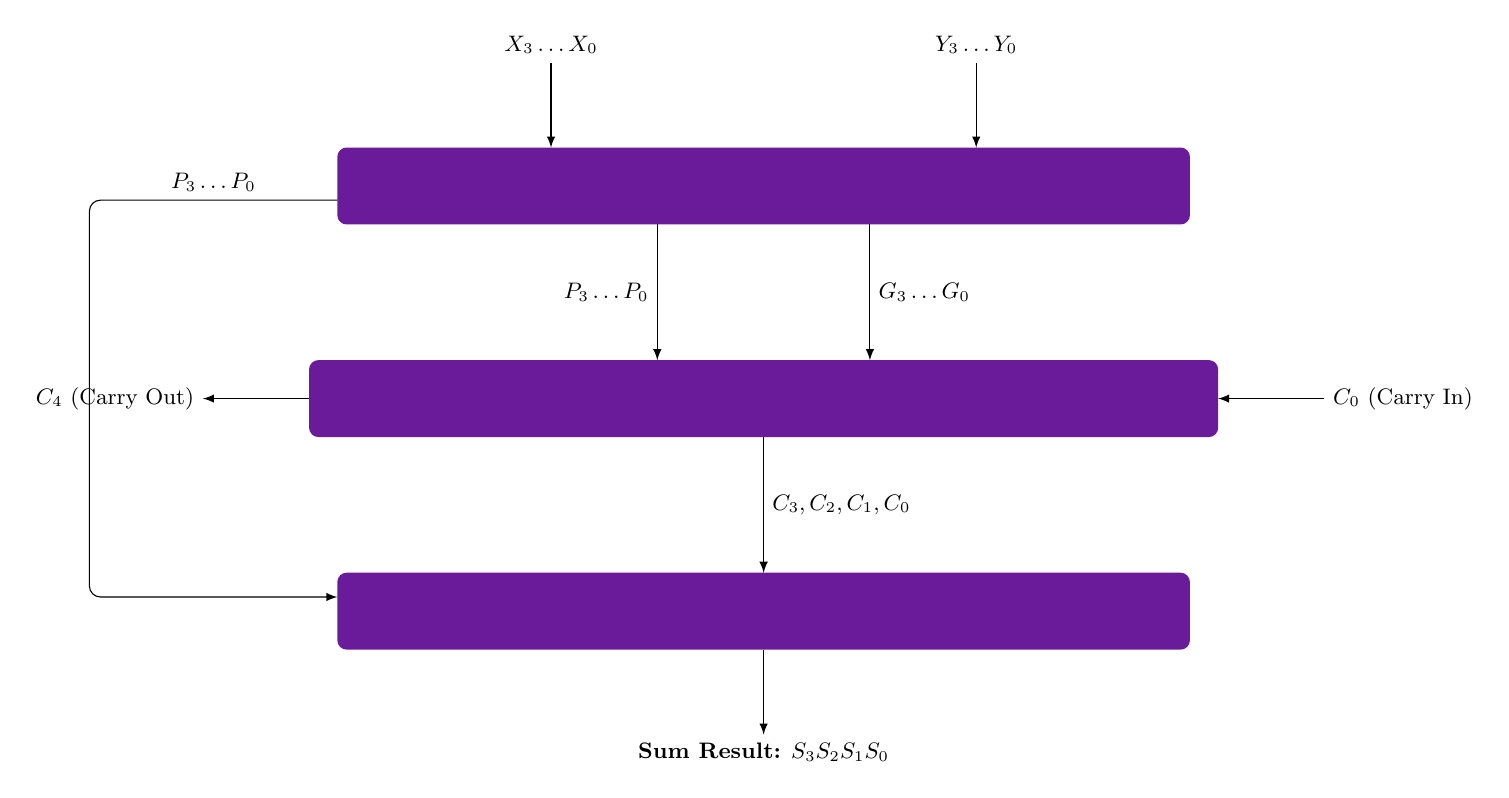
\begin{tikzpicture}[>=latex, node distance=3cm, scale=0.9, transform shape, font=\small]

    \tikzstyle{block} = [draw, rectangle, minimum height=3em, minimum width=12cm, text centered, fill=blue!10, rounded corners=3pt, thick, cD]
    
    % Stage 1
    \node[block] (pg) {\textbf{Stage 1: P \& G Generator} $\quad (P_i = X_i \oplus Y_i, \quad G_i = X_i \cdot Y_i)$};
    
    % Stage 2
    \node[block, below of=pg] (cla) {\textbf{Stage 2: Carry Look-Ahead Generator} $\quad (\text{Computes } C_1, C_2, C_3, C_4 \text{ via SOP logic})$};
    
    % Stage 3
    \node[block, below of=cla] (sum) {\textbf{Stage 3: Sum Generator} $\quad (S_i = P_i \oplus C_i)$};
    
    % Inputs Top
    \draw[<-] ([xshift=-3cm]pg.north) -- ++(0, 1.2) node[above] {$X_3 \dots X_0$};
    \draw[<-] ([xshift=3cm]pg.north) -- ++(0, 1.2) node[above] {$Y_3 \dots Y_0$};
    
    % P and G from Stage 1 to Stage 2
    \draw[->] ([xshift=-1.5cm]pg.south) -- ([xshift=-1.5cm]cla.north) node[midway, left] {$P_3 \dots P_0$};
    \draw[->] ([xshift=1.5cm]pg.south) -- ([xshift=1.5cm]cla.north) node[midway, right] {$G_3 \dots G_0$};
    
    % Carries from Stage 2 to Stage 3
    \draw[->] (cla.south) -- (sum.north) node[midway, right] {$C_3, C_2, C_1, C_0$};
    
    % P from Stage 1 bypass to Stage 3 (Routed wider to completely avoid C4)
    \draw[->, rounded corners] ([yshift=-2mm]pg.west) -- ++(-3.5,0) node[midway, above] {$P_3 \dots P_0$} |- ([yshift=2mm]sum.west);
    
    % Carry In
    \draw[<-] (cla.east) -- ++(1.5, 0) node[right] {$C_0$ (Carry In)};
    
    % Carry Out
    \draw[->] (cla.west) -- ++(-1.5, 0) node[left] {$C_4$ (Carry Out)};
    
    % Sum Out
    \draw[->] (sum.south) -- ++(0, -1.2) node[below] {\textbf{Sum Result:} $S_3 S_2 S_1 S_0$};
\end{tikzpicture}
\end{center}

\vspace{0.5em}
\textbf{Conclusion on the Role of Carries:}
In this architecture, the $C_1, C_2, C_3,$ and $C_4$ logic gates (comprising Stage 2) are completely decoupled from the $S_i$ calculations of preceding bits. They serve the critical role of flattening the serial propagation path. By utilizing direct inputs and pre-computed $P_i$ and $G_i$ values, they feed the correct carry bit into Stage 3 almost instantaneously, empowering the adder to process the 4-bit numbers at a fraction of the time required by standard adders.

\end{tcolorbox}

\item Design a 3-bit CLA circuit and show all types of ``carry'' for the addition $3+4$ with your designed CLA.
\mk{8+4} \yr{CSE 205 | L-2/T-1 | 2017--18}

\begin{tcolorbox}[enhanced,breakable,ansbox,colback=cD!4,colframe=cD,boxrule=0.8pt,arc=5pt,title={\textbf{Answer}},fonttitle=\bfseries\color{white},colbacktitle=cD]

A Carry Lookahead Adder (CLA) significantly reduces carry propagation delay by computing carries in parallel using early generated and propagated carry signals. 

\subsubsection*{1. Mathematical Derivation for a 3-bit CLA}
For any bit position $i$, the logic evaluates two intermediate signals:
\begin{itemize}
    \item \textbf{Propagate Carry} ($\mathbf{P_i}$): Indicates if an incoming carry will be passed to the next bit. $P_i = A_i \oplus B_i$
    \item \textbf{Generate Carry} ($\mathbf{G_i}$): Indicates if a carry is directly created at this bit regardless of the incoming carry. $G_i = A_i \cdot B_i$
\end{itemize}
The sum and lookahead carry equations are given by:
\begin{align*}
    S_i &= P_i \oplus C_i \\
    C_{i+1} &= G_i + P_i \cdot C_i
\end{align*}
Unrolling the carry equations for a 3-bit adder yields the \textbf{Carry Lookahead logic}:
\begin{align*}
    \text{\textbf{Carry 1:}} \quad C_1 &= G_0 + P_0C_0 \\
    \text{\textbf{Carry 2:}} \quad C_2 &= G_1 + P_1C_1 \\
                                       &= G_1 + P_1(G_0 + P_0C_0) \\
                                       &= G_1 + P_1G_0 + P_1P_0C_0 \\
    \text{\textbf{Carry 3:}} \quad C_3 &= G_2 + P_2C_2 \\
                                       &= G_2 + P_2(G_1 + P_1G_0 + P_1P_0C_0) \\
                                       &= G_2 + P_2G_1 + P_2P_1G_0 + P_2P_1P_0C_0
\end{align*}

\vspace{0.5cm}
\subsubsection*{2. 3-Bit CLA Circuit Design}
Below is the gate-level implementation of the \textbf{Carry Lookahead Generator} that computes $C_1, C_2$, and $C_3$ in parallel.

\begin{center}
\begin{circuitikz}[scale=0.9, transform shape, thick]
    
    % --- C1 Logic ---
    \node[or port] (o1) at (7, 0) {};
    \node[and port] (a11) at (4, -0.6) {};
    
    \draw (o1.in 1) -- ++(-6,0) node[left] {$G_0$};
    \draw (a11.in 1) -- ++(-3,0) node[left] {$P_0$};
    \draw (a11.in 2) -- ++(-3,0) node[left] {$C_0$};
    \draw (a11.out) |- (o1.in 2);
    \draw (o1.out) -- ++(1,0) node[right, font=\bfseries] {$C_1$};

    % --- C2 Logic ---
    \node[or port, number inputs=3] (o2) at (7, -3.5) {};
    \node[and port] (a21) at (4, -3.5) {};
    \node[and port, number inputs=3] (a22) at (4, -4.8) {};

    \draw (o2.in 1) -- ++(-1,0) --++(0, 1) --++(-5,0) node[left] {$G_1$};
    
    \draw (a21.in 1) -- ++(-3,0) node[left] {$P_1$};
    \draw (a21.in 2) -- ++(-3,0) node[left] {$G_0$};
    
    \draw (a22.in 1) -- ++(-3,0) node[left] {$P_1$};
    \draw (a22.in 2) -- ++(-3,0) node[left] {$P_0$};
    \draw (a22.in 3) -- ++(-3,0) node[left] {$C_0$};
    
    \draw (a21.out) |- (o2.in 2);
    \draw (a22.out) |- (o2.in 3);
    \draw (o2.out) -- ++(1,0) node[right, font=\bfseries] {$C_2$};

    % --- C3 Logic ---
    \node[or port, number inputs=4] (o3) at (7, -8) {};
    \node[and port] (a31) at (4, -7.5) {};
    \node[and port, number inputs=3] (a32) at (4, -8.8) {};
    \node[and port, number inputs=4] (a33) at (4, -10.3) {};

    \draw (o3.in 1) -- ++(-1,0) --++(0,1)--++(-5,0) node[left] {$G_2$};
    
    \draw (a31.in 1) -- ++(-3,0) node[left] {$P_2$};
    \draw (a31.in 2) -- ++(-3,0) node[left] {$G_1$};
    
    \draw (a32.in 1) -- ++(-3,0) node[left] {$P_2$};
    \draw (a32.in 2) -- ++(-3,0) node[left] {$P_1$};
    \draw (a32.in 3) -- ++(-3,0) node[left] {$G_0$};
    
    \draw (a33.in 1) -- ++(-3,0) node[left] {$P_2$};
    \draw (a33.in 2) -- ++(-3,0) node[left] {$P_1$};
    \draw (a33.in 3) -- ++(-3,0) node[left] {$P_0$};
    \draw (a33.in 4) -- ++(-3,0) node[left] {$C_0$};
    
    \draw (a31.out) |- (o3.in 2);
    \draw (a32.out) |- (o3.in 3);
    \draw (a33.out)--++(1,0) |- (o3.in 4);
    \draw (o3.out) -- ++(1,0) node[right, font=\bfseries] {$C_3$};
\end{circuitikz}
\end{center}

The fully integrated structural top-level design incorporates the initial PG Generators, the CLA unit (designed above), and the final Sum XOR gates:

\begin{center}
\begin{circuitikz}[scale=0.85, transform shape, thick]


    % ================= CLA Block Background =================
    \draw[fill=cD!5, rounded corners, draw=cD] (5, 2.5) rectangle (8.5, -9);
    \node[font=\large\bfseries, text=cD, align=center] at (6.75, -3.25) {3-Bit Carry\\Look-Ahead\\Generator};
    
    % ================= Initial Carry C0 =================
    \draw (0, 1.8) node[left] {$C_0$} -- (5, 1.8) node[pos=0.85, above] {$C_0$};

    % ================= 3-Bit Logic Loops =================
    \foreach \i/\y in {0/0, 1/-3.5, 2/-7} {
        
        % --- P and G Generators (Left Side) ---
        \node[xor port, scale=0.8] (pgx\i) at (3, \y+0.8) {};
        \node[and port, scale=0.8] (pga\i) at (3, \y-0.8) {};
        
        % Inputs A_i, B_i
        \draw (0, |- pgx\i.in 1) node[left] {$A_\i$} -- (pgx\i.in 1);
        \draw (0, |- pga\i.in 2) node[left] {$B_\i$} -- (pga\i.in 2);
        
        % Tapping inputs for P and G
        \draw (1.0, |- pgx\i.in 1) coordinate (tapA\i);
        \fill (tapA\i) circle (1.5pt);
        \draw (tapA\i) |- (pga\i.in 1);
        
        \draw (1.5, |- pga\i.in 2) coordinate (tapB\i);
        \fill (tapB\i) circle (1.5pt);
        \draw (tapB\i) |- (pgx\i.in 2);

        % Connect P and G to CLA Block
        \draw (pgx\i.out) -- (5, |- pgx\i.out) node[pos=0.5, above] {$P_\i$};
        \draw (pga\i.out) -- (5, |- pga\i.out) node[pos=0.5, below] {$G_\i$};

        % --- Sum Generators (Right Side) ---
        \node[xor port, scale=0.8] (sum\i) at (10.5, \y) {};
        
        % Output Carries and Propagates from CLA to Sum Gates
        \draw (8.5, |- sum\i.in 1) -- (sum\i.in 1) node[pos=0.4, above] {$P_\i$};
        \draw (8.5, |- sum\i.in 2) -- (sum\i.in 2) node[pos=0.4, below] {$C_\i$};
        
        % Final Sum Output
        \draw (sum\i.out) -- (12, |- sum\i.out) node[right, font=\bfseries] {$S_\i$};
    }

    % ================= Final Carry Out C3 =================
    \draw (8.5, -8.3) -- (12, -8.3) node[right, font=\bfseries] {$C_3$ ($C_{out}$)};

\end{circuitikz}
\end{center}

\vspace{0.3cm}
\subsubsection*{3. Application: Adding $3 + 4$}
We are performing the addition $A + B$, where:
\begin{itemize}
    \item $A = 3_{10} = 011_2 \implies A_2=0, A_1=1, A_0=1$
    \item $B = 4_{10} = 100_2 \implies B_2=1, B_1=0, B_0=0$
    \item Assume an initial carry input $C_0 = 0$.
\end{itemize}

\textbf{Step 1: Calculate Generate ($G_i$) and Propagate ($P_i$) Carries}
\begin{align*}
    \text{Bit 0:} \quad P_0 &= A_0 \oplus B_0 = 1 \oplus 0 = \mathbf{1} & G_0 &= A_0 \cdot B_0 = 1 \cdot 0 = \mathbf{0} \\
    \text{Bit 1:} \quad P_1 &= A_1 \oplus B_1 = 1 \oplus 0 = \mathbf{1} & G_1 &= A_1 \cdot B_1 = 1 \cdot 0 = \mathbf{0} \\
    \text{Bit 2:} \quad P_2 &= A_2 \oplus B_2 = 0 \oplus 1 = \mathbf{1} & G_2 &= A_2 \cdot B_2 = 0 \cdot 1 = \mathbf{0} 
\end{align*}

\textbf{Step 2: Calculate Internal Lookahead Carries ($C_i$)}
\begin{align*}
    C_1 &= G_0 + P_0C_0 = 0 + (1 \cdot 0) = \mathbf{0} \\
    C_2 &= G_1 + P_1C_1 = 0 + (1 \cdot 0) = \mathbf{0} \\
    C_3 &= G_2 + P_2C_2 = 0 + (1 \cdot 0) = \mathbf{0} 
\end{align*}
\textit{Note:} Because bits of A and B do not simultaneously contain `1` in any position, $G_i=0$ across all bits. As the starting carry $C_0=0$, there are no incoming carries to propagate either. Thus, all internal lookahead carries evaluate to zero.

\textbf{Step 3: Calculate Final Sum ($S_i$)}
\begin{align*}
    S_0 &= P_0 \oplus C_0 = 1 \oplus 0 = \mathbf{1} \\
    S_1 &= P_1 \oplus C_1 = 1 \oplus 0 = \mathbf{1} \\
    S_2 &= P_2 \oplus C_2 = 1 \oplus 0 = \mathbf{1} 
\end{align*}

\textbf{Summary of all signal types (Showing all ``carries''):}
\begin{center}
\renewcommand{\arraystretch}{1.3}
\begin{tabular}{c c c | c c | c | c}
\toprule
\textbf{Bit ($i$)} & \textbf{$A_i$} & \textbf{$B_i$} & \textbf{Generate ($G_i$)} & \textbf{Propagate ($P_i$)} & \textbf{Carry In ($C_i$)} & \textbf{Sum ($S_i$)} \\
\midrule
0 & 1 & 0 & 0 & 1 & $C_0 = 0$ & 1 \\
1 & 1 & 0 & 0 & 1 & $C_1 = 0$ & 1 \\
2 & 0 & 1 & 0 & 1 & $C_2 = 0$ & 1 \\
\midrule
\multicolumn{6}{r|}{\textbf{Final Carry Out ($C_3$)}} & \textbf{0} \\
\bottomrule
\end{tabular}
\end{center}
\textbf{Final Result:} $C_3 S_2 S_1 S_0 = 0111_2 = \mathbf{7_{10}}$.

\end{tcolorbox}

\item For a carry look-ahead adder circuit, what advantage do we get if we use it instead of a 4-bit simple full adder? For a NOT gate with 2\,ns propagation delay and other basic gates with 4\,ns propagation delay, what will be the total propagation delay?
\mk{5} \yr{CSE 205 | L-2/T-1 | 2016--17}

\begin{tcolorbox}[enhanced,breakable,ansbox,colback=cD!4,colframe=cD,boxrule=0.8pt,arc=5pt,title={\textbf{Answer}},fonttitle=\bfseries\color{white},colbacktitle=cD]

\subsubsection*{Part 1: Advantage of a Carry Look-Ahead Adder (CLA)}

In a simple 4-bit full adder (often called a \textbf{Ripple Carry Adder} or RCA), the carry bit ripples from the least significant bit (LSB) to the most significant bit (MSB). Consequently, the sum for bit $i$ cannot be computed until the carry-out from bit $i-1$ is ready. This creates a linear propagation delay, $O(n)$, which becomes unacceptably slow for larger bit-widths.

The primary advantage of the \textbf{Carry Look-Ahead Adder (CLA)} is that it completely eliminates this ripple effect. By calculating intermediary \textbf{Generate ($G_i$)} and \textbf{Propagate ($P_i$)} signals, the CLA computes all carry signals ($C_1, C_2, C_3, C_4$) \textbf{in parallel} using 2-level Sum-of-Products (SOP) logic. 
\begin{itemize}
    \item \textbf{Speed:} The carry generation delay becomes constant (theoretical $O(1)$ gate levels), drastically reducing the overall addition time.
    \item \textbf{Independence:} Each carry bit is calculated directly from the inputs ($A, B$) and the initial carry-in ($C_0$), without waiting for the intermediate sum/carry of preceding bits.
\end{itemize}

\vspace{0.3cm}
\hrule
\vspace{0.3cm}

\subsubsection*{Part 2: Total Propagation Delay Calculation}

The problem explicitly provides the delay of a NOT gate ($2\,$ns) and other basic gates ($4\,$ns). Standard ``basic gates'' include AND and OR gates. Because the NOT gate delay is distinctly specified, we must decompose the XOR gate (which is a derived gate) into its constituent basic gates to accurately trace the delay.

\paragraph{1. Delay of an XOR Gate}
The XOR operation $X \oplus Y = X\bar{Y} + \bar{X}Y$ is constructed using NOT, AND, and OR gates:
\begin{align*}
    \text{NOT gates ($\bar{X}, \bar{Y}$ delay):} &\quad 2\text{ ns} \\
    \text{AND layer ($X\bar{Y}, \bar{X}Y$ delay):} &\quad 2\text{ ns} + 4\text{ ns} = 6\text{ ns} \\
    \text{OR layer (Final XOR delay):} &\quad 6\text{ ns} + 4\text{ ns} = \mathbf{10\text{ ns}}
\end{align*}
Thus, any XOR operation introduces a $10\,$ns delay from the time its latest input is available.

\paragraph{2. Stage-by-Stage Delay Trace for the CLA}
Assume all primary inputs ($A_i, B_i, C_0$) arrive simultaneously at $t = 0\,$ns.

\textbf{Stage 1: Generate ($G_i$) and Propagate ($P_i$) Signals} \\
The signals are computed in parallel for all bits:
\begin{align*}
    G_i &= A_i \cdot B_i \quad &\text{(1 AND gate)} \implies \text{Valid at } t &= 0 + 4 = \mathbf{4\text{ ns}} \\
    P_i &= A_i \oplus B_i \quad &\text{(1 XOR logic)} \implies \text{Valid at } t &= 0 + 10 = \mathbf{10\text{ ns}}
\end{align*}

\textbf{Stage 2: Carry Look-Ahead Logic ($C_i$)} \\
The carry bits are evaluated using 2-level AND-OR logic. For example, $C_4$:
\[
    C_4 = G_3 + P_3G_2 + P_3P_2G_1 + P_3P_2P_1G_0 + P_3P_2P_1P_0C_0
\]
\begin{itemize}
    \item The inputs to this block are the $G_i$ signals (arriving at $4\,$ns) and $P_i$ signals (arriving at $10\,$ns).
    \item \textbf{AND Layer:} Must wait for the slowest input, which is $P_i$ at $10\,$ns. \\
          Outputs of the AND gates are valid at $t = 10\text{ ns} + 4\text{ ns} = \mathbf{14\text{ ns}}$.
    \item \textbf{OR Layer:} Takes the outputs of the AND layer. \\
          Outputs of the OR gates (all $C_i$) are valid at $t = 14\text{ ns} + 4\text{ ns} = \mathbf{18\text{ ns}}$.
\end{itemize}

\textbf{Stage 3: Final Sum Generation ($S_i$)} \\
The sum is computed as $S_i = P_i \oplus C_i = P_i \bar{C}_i + \bar{P}_i C_i$. \\
We track the arrival times of the inputs to this final XOR logic:
\begin{itemize}
    \item $P_i$ is available at $10\,$ns.
    \item $C_i$ is available at $18\,$ns.
    \item \textbf{NOT Layer:} Computes $\bar{P}_i$ and $\bar{C}_i$. 
    \begin{itemize}
        \item $\bar{P}_i$ is valid at $10\text{ ns} + 2\text{ ns} = 12\text{ ns}$.
        \item $\bar{C}_i$ is valid at $18\text{ ns} + 2\text{ ns} = \mathbf{20\text{ ns}}$.
    \end{itemize}
    \item \textbf{AND Layer ($P_i \bar{C}_i$ and $\bar{P}_i C_i$):} The slowest input is $\bar{C}_i$ at $20\,$ns. \\
          The AND gates evaluate at $t = 20\text{ ns} + 4\text{ ns} = \mathbf{24\text{ ns}}$.
    \item \textbf{OR Layer (Final Sum):} \\
          The final OR gate evaluates at $t = 24\text{ ns} + 4\text{ ns} = \textcolor{cD}{\textbf{28\text{ ns}}}$.
\end{itemize}

\vspace{0.2cm}
\textbf{Conclusion:} 
The total propagation delay to compute the final sum and carry-out in this Carry Look-Ahead Adder is \textcolor{cD}{\textbf{28\,ns}}.

\vspace{0.2cm}
\hrule
\vspace{0.2cm}
\footnotesize
\textit{Note:} If a simpler architecture is assumed where the XOR gate is treated intrinsically as a standard basic gate with a $4\,$ns delay (ignoring the provided NOT gate delay parameter), the calculation simplifies to: $P_i$ ready at $4\,$ns $\to$ Carry ANDs at $8\,$ns $\to$ Carry ORs at $12\,$ns $\to$ Final Sum XOR at $16\,$ns. However, utilizing the explicitly provided NOT delay requires the standard decomposition shown above.

\end{tcolorbox}

\item What is the problem with the binary parallel adder circuit? Design and implement a 4-bit carry look-ahead adder circuit. If the propagation delay is 1\,ns for a NOT gate and 2\,ns for other basic gates, what is the propagation delay of the CLA adder to produce its final output?
\mk{18} \yr{CSE 205 | L-2/T-1 | 2015--16}

\begin{tcolorbox}[enhanced,breakable,ansbox,colback=cD!4,colframe=cD,boxrule=0.8pt,arc=5pt,title={\textbf{Answer}},fonttitle=\bfseries\color{white},colbacktitle=cD]

\subsubsection*{1. The Problem with the Binary Parallel Adder}

A standard Binary Parallel Adder (also known as a \textbf{Ripple Carry Adder} or RCA) cascades multiple 1-bit full adders to add $n$-bit numbers. The primary problem with this architecture is the \textbf{carry propagation delay}. 
In an RCA, the sum $S_i$ and the carry-out $C_{i+1}$ for any bit position $i$ cannot be correctly computed until the carry-in $C_i$ from the previous stage has been evaluated. Consequently, the carry must ``ripple'' sequentially from the least significant bit (LSB) to the most significant bit (MSB). For an $n$-bit adder, the worst-case propagation delay is $O(n)$, which acts as a major bottleneck in high-speed computing systems.

\vspace{0.3cm}
\subsubsection*{2. Design and Implementation of a 4-Bit Carry Look-Ahead Adder}

A Carry Look-Ahead Adder (CLA) solves the ripple delay by computing all carry signals simultaneously using two intermediate signals for each bit:
\begin{itemize}
    \item \textbf{Generate ($G_i = A_i \cdot B_i$):} Produces a carry out regardless of the carry in.
    \item \textbf{Propagate ($P_i = A_i \oplus B_i$):} Propagates a carry in to the carry out.
\end{itemize}
The standard sum and carry formulas are:
\begin{align*}
    S_i &= P_i \oplus C_i \\
    C_{i+1} &= G_i + P_i \cdot C_i
\end{align*}
By unrolling the carry equations, we derive independent carry logic for the 4-bit CLA:
\begin{align*}
    C_1 &= G_0 + P_0C_0 \\
    C_2 &= G_1 + P_1C_1 = G_1 + P_1G_0 + P_1P_0C_0 \\
    C_3 &= G_2 + P_2C_2 = G_2 + P_2G_1 + P_2P_1G_0 + P_2P_1P_0C_0 \\
    C_4 &= G_3 + P_3C_3 = G_3 + P_3G_2 + P_3P_2G_1 + P_3P_2P_1G_0 + P_3P_2P_1P_0C_0
\end{align*}

\textbf{Structural Block Diagram of the 4-Bit CLA:}

\vspace{0.3cm}
\begin{center}
\begin{circuitikz}[scale=0.85, transform shape, thick]



    % ================= CLA Block Background =================
    \draw[fill=cD!5, rounded corners, draw=cD] (5, 2.5) rectangle (8.5, -12.5);
    \node[font=\large\bfseries, text=cD, align=center] at (6.75, -5.25) {4-Bit Carry\\Look-Ahead\\Generator};
    \node[align=center, font=\footnotesize] at (6.75, -6.75) {(Implements\\SOP Logic for\\$C_1, C_2, C_3, C_4$)};

    % ================= Initial Carry C0 =================
    \draw (0, 1.8) node[left] {$C_0$} -- (5, 1.8) node[pos=0.85, above] {$C_0$};

    % ================= 4-Bit Logic Loops =================
    \foreach \i/\y in {0/0, 1/-3.5, 2/-7, 3/-10.5} {
        
        % --- P and G Generators (Left Side) ---
        \node[xor port, scale=0.8] (pgx\i) at (3, \y+0.8) {};
        \node[and port, scale=0.8] (pga\i) at (3, \y-0.8) {};
        
        % Inputs A_i, B_i
        \draw (0, |- pgx\i.in 1) node[left] {$A_\i$} -- (pgx\i.in 1);
        \draw (0, |- pga\i.in 2) node[left] {$B_\i$} -- (pga\i.in 2);
        
        % Tapping inputs for P and G
        \draw (1.0, |- pgx\i.in 1) coordinate (tapA\i);
        \fill (tapA\i) circle (1.5pt);
        \draw (tapA\i) |- (pga\i.in 1);
        
        \draw (1.5, |- pga\i.in 2) coordinate (tapB\i);
        \fill (tapB\i) circle (1.5pt);
        \draw (tapB\i) |- (pgx\i.in 2);

        % Connect P and G to CLA Block
        \draw (pgx\i.out) -- (5, |- pgx\i.out) node[pos=0.5, above] {$P_\i$};
        \draw (pga\i.out) -- (5, |- pga\i.out) node[pos=0.5, below] {$G_\i$};

        % --- Sum Generators (Right Side) ---
        \node[xor port, scale=0.8] (sum\i) at (10.5, \y) {};
        
        % Output Carries and Propagates from CLA to Sum Gates
        \draw (8.5, |- sum\i.in 1) -- (sum\i.in 1) node[pos=0.4, above] {$P_\i$};
        \draw (8.5, |- sum\i.in 2) -- (sum\i.in 2) node[pos=0.4, below] {$C_\i$};
        
        % Final Sum Output
        \draw (sum\i.out) -- (12, |- sum\i.out) node[right, font=\bfseries] {$S_\i$};
    }

    % ================= Final Carry Out C4 =================
    \draw (8.5, -11.8) -- (12, -11.8) node[right, font=\bfseries] {$C_4$ ($C_{out}$)};

\end{circuitikz}
\end{center}

\vspace{0.3cm}
\subsubsection*{3. Propagation Delay Calculation}

We are given the delay of a \textbf{NOT gate ($1\,$ns)} and \textbf{other basic gates ($2\,$ns)} (i.e., AND/OR gates). 
Because the NOT gate delay is specifically provided, we must decompose the complex XOR gates into their basic gate equivalents: $X \oplus Y = X\bar{Y} + \bar{X}Y$.
\begin{align*}
    \text{NOT layer ($\bar{X}, \bar{Y}$):} &\quad 1\text{ ns} \\
    \text{AND layer ($X\bar{Y}, \bar{X}Y$):} &\quad 1\text{ ns} + 2\text{ ns} = 3\text{ ns} \\
    \text{OR layer (Final XOR delay):} &\quad 3\text{ ns} + 2\text{ ns} = \mathbf{5\text{ ns}}
\end{align*}
Thus, an XOR operation yields a delay of $5\text{ ns}$. Now, assuming all inputs ($A_i, B_i, C_0$) arrive at $t = 0\text{ ns}$, we trace the CLA critical path:

\paragraph{Stage 1: Generate ($G_i$) and Propagate ($P_i$) Signals}
\begin{itemize}
    \item $G_i = A_i \cdot B_i$ uses 1 AND gate $\implies$ Ready at $t = 0 + 2 = \mathbf{2\text{ ns}}$.
    \item $P_i = A_i \oplus B_i$ uses 1 XOR gate $\implies$ Ready at $t = 0 + 5 = \mathbf{5\text{ ns}}$.
\end{itemize}

\paragraph{Stage 2: Carry Look-Ahead Logic ($C_1, C_2, C_3, C_4$)}
The logic evaluates 2-level Sum-of-Products (SOP) equations (AND gates followed by OR gates).
\begin{itemize}
    \item \textbf{AND Layer:} Takes inputs $G_i$ (2 ns), $P_i$ (5 ns), and $C_0$ (0 ns). It must wait for the slowest input ($P_i$ at 5 ns). \\
          Output of AND layer $\implies 5\text{ ns} + 2\text{ ns} = \mathbf{7\text{ ns}}$.
    \item \textbf{OR Layer:} Takes the output of the AND layer. \\
          Output of OR layer (all $C_i$ and $C_4$) $\implies 7\text{ ns} + 2\text{ ns} = \mathbf{9\text{ ns}}$.
\end{itemize}
\textit{(Note: The final carry out $C_4$ is completely evaluated and valid at \textbf{9\,ns}.)}

\paragraph{Stage 3: Final Sum Generation ($S_i$)}
The final sum is $S_i = P_i \oplus C_i = P_i \bar{C}_i + \bar{P}_i C_i$.
\begin{itemize}
    \item \textbf{Inputs Available:} $P_i$ is ready at 5 ns, and $C_i$ is ready at 9 ns.
    \item \textbf{NOT Layer:} $\bar{P}_i$ is ready at $5 + 1 = 6\text{ ns}$, and $\bar{C}_i$ is ready at $9 + 1 = \mathbf{10\text{ ns}}$.
    \item \textbf{AND Layer:} Must wait for the slowest input ($\bar{C}_i$ at 10 ns). \\
          Evaluation finishes at $t = 10\text{ ns} + 2\text{ ns} = \mathbf{12\text{ ns}}$.
    \item \textbf{OR Layer:} Generates the final Sum. \\
          Evaluation finishes at $t = 12\text{ ns} + 2\text{ ns} = \textcolor{cD}{\textbf{14\text{ ns}}}$.
\end{itemize}

\vspace{0.2cm}
\textbf{Conclusion:} 
The propagation delay for the CLA adder to produce its final output (the final Sum bit) is \textcolor{cD}{\textbf{14\,ns}}. 

\end{tcolorbox}

\item What are the advantages of a CLA over a normal binary four-bit adder? Assume that the exclusive-OR gate has a propagation delay of 10\,ns and that the AND or OR gates have a propagation delay of 5\,ns. What is the total propagation delay time in the four-bit CLA adder?
\mk{10} \yr{CSE 205 | L-2/T-1 | 2013--14}

\begin{tcolorbox}[enhanced,breakable,ansbox,colback=cD!4,colframe=cD,boxrule=0.8pt,arc=5pt,title={\textbf{Answer}},fonttitle=\bfseries\color{white},colbacktitle=cD]

\subsubsection*{1. Advantages of a CLA over a Normal Binary Four-Bit Adder}

A ``normal'' binary four-bit adder, typically implemented as a \textbf{Ripple Carry Adder (RCA)}, cascades single-bit full adders in a series. The primary advantages of replacing this with a \textbf{Carry Look-Ahead Adder (CLA)} are:

\begin{itemize}
    \item \textbf{Elimination of the Ripple Effect:} In an RCA, the carry propagates sequentially from the LSB to the MSB, resulting in a linear delay $O(n)$. A CLA precomputes the carry signals in parallel using Generate ($G_i$) and Propagate ($P_i$) logic, ensuring that the MSB does not have to wait for the carry to ripple through all preceding bits.
    \item \textbf{Constant Carry Delay:} Regardless of the bit-width of the adder block (up to a fan-in limit), the carry outputs ($C_1, C_2, C_3, C_4$) are generated simultaneously via a 2-level Sum-of-Products (SOP) circuit. This significantly boosts the clock speed capability of the CPU's Arithmetic Logic Unit (ALU).
    \item \textbf{Faster Overall Addition:} Because the carries arrive much earlier, the final Sum ($S_i = P_i \oplus C_i$) bits are also evaluated much faster compared to a standard RCA.
\end{itemize}

\vspace{0.3cm}
\hrule
\vspace{0.3cm}

\subsubsection*{2. Total Propagation Delay Calculation}

We are given the following inherent gate delays:
\begin{itemize}
    \item \textbf{XOR gate delay:} $10\text{ ns}$
    \item \textbf{AND gate delay:} $5\text{ ns}$
    \item \textbf{OR gate delay:} $5\text{ ns}$
\end{itemize}
Assume all primary inputs ($A_i, B_i$, and initial carry $C_0$) are applied simultaneously at $t = 0\text{ ns}$. The calculation proceeds stage by stage based on the critical path of the CLA architecture.

\paragraph{Stage 1: Generate ($G_i$) and Propagate ($P_i$) Signals}
For each bit $i$, these signals are calculated directly from the inputs in parallel:
\begin{align*}
    G_i &= A_i \cdot B_i &\quad (\text{1 AND gate}) \implies \text{Valid at } t &= 0 + 5 = \mathbf{5\text{ ns}} \\
    P_i &= A_i \oplus B_i &\quad (\text{1 XOR gate}) \implies \text{Valid at } t &= 0 + 10 = \mathbf{10\text{ ns}}
\end{align*}

\paragraph{Stage 2: Carry Look-Ahead Logic ($C_1, C_2, C_3, C_4$)}
The look-ahead logic utilizes a 2-level AND-OR structure (Sum-of-Products) for all carries. For example, the longest expression is:
\[
    C_4 = G_3 + P_3G_2 + P_3P_2G_1 + P_3P_2P_1G_0 + P_3P_2P_1P_0C_0
\]
\begin{itemize}
    \item \textbf{AND Layer:} The inputs to the AND gates are $G_i$ (arriving at $5\text{ ns}$), $P_i$ (arriving at $10\text{ ns}$), and $C_0$ ($0\text{ ns}$). The AND gates must wait for the slowest input, which is $P_i$ at $10\text{ ns}$. \\
    Evaluating the AND gates adds $5\text{ ns}$: \quad $t = 10\text{ ns} + 5\text{ ns} = \mathbf{15\text{ ns}}$.
    
    \item \textbf{OR Layer:} The OR gates sum the outputs of the AND layer (which arrive at $15\text{ ns}$) and the standalone $G_i$ signals (which arrive early at $5\text{ ns}$). It waits for the slowest input at $15\text{ ns}$. \\
    Evaluating the OR gates adds $5\text{ ns}$: \quad $t = 15\text{ ns} + 5\text{ ns} = \mathbf{20\text{ ns}}$.
\end{itemize}
\textit{All internal carry bits ($C_1, C_2, C_3$) and the final carry-out ($C_4$) are valid at $20\text{ ns}$.}

\paragraph{Stage 3: Final Sum Generation ($S_i$)}
The final sum for each bit is calculated using the equation:
\[
    S_i = P_i \oplus C_i
\]
\begin{itemize}
    \item \textbf{Inputs:} The XOR gate receives $P_i$ (ready at $10\text{ ns}$) and $C_i$ (ready at $20\text{ ns}$).
    \item \textbf{Evaluation:} The XOR gate must wait for the slowest input, which is $C_i$ at $20\text{ ns}$. \\
    Evaluating the XOR gate adds $10\text{ ns}$: \quad $t = 20\text{ ns} + 10\text{ ns} = \textcolor{cD}{\textbf{30\text{ ns}}}$.
\end{itemize}

\vspace{0.2cm}
\textbf{Conclusion:} \\
The total propagation delay time for the four-bit CLA adder to stabilize all outputs (including the Sum bits and the final Carry-out) is \textcolor{cD}{\textbf{30\,ns}}.

\end{tcolorbox}

\end{enumerate}

%%──────────────────────────────────────────────────────────────────────
\subtopic{cD}{2's Complement Circuit}
\label{sub:s4-2scomp}

\begin{enumerate}


\item Using only half adders, design a circuit that outputs the 1's complement of a 4-bit input when the control input $C$ is 1, and passes the input unchanged when $C$ is 0.
\mk{6} \yr{CSE 205 | L-2/T-1 | 2023--24}

\begin{tcolorbox}[enhanced,breakable,ansbox,colback=cD!4,colframe=cD,boxrule=0.8pt,arc=5pt,title={\textbf{Answer}},fonttitle=\bfseries\color{white},colbacktitle=cD]

\subsubsection*{1. Logical Analysis and Formulation}
Let the 4-bit input be $A = A_3 A_2 A_1 A_0$ and the required 4-bit output be $Y = Y_3 Y_2 Y_1 Y_0$. We are given a control signal $C$ which determines the operation:
\begin{itemize}
    \item When $C = 0$, the output passes the input unchanged: $Y_i = A_i$.
    \item When $C = 1$, the output is the 1's complement of the input: $Y_i = A_i'$.
\end{itemize}

We can formulate the truth table for a single bit $i$ (where $i \in \{0,1,2,3\}$):

\begin{center}
\renewcommand{\arraystretch}{1.2}
\begin{tabular}{cc|c|l}
\toprule
\textbf{Control ($C$)} & \textbf{Input ($A_i$)} & \textbf{Desired Output ($Y_i$)} & \textbf{Description} \\
\midrule
0 & 0 & 0 & \multirow{2}{*}{Pass Unchanged ($Y_i = A_i$)} \\
0 & 1 & 1 & \\
\midrule
1 & 0 & 1 & \multirow{2}{*}{1's Complement ($Y_i = A_i'$)} \\
1 & 1 & 0 & \\
\bottomrule
\end{tabular}
\end{center}

Extracting the Boolean expression from the truth table via sum-of-products for $Y_i$, we get:
\begin{align*}
    Y_i &= C'A_i + CA_i' \\
    Y_i &= C \oplus A_i \quad \textcolor{cD}{\text{(Exclusive-OR Operation)}}
\end{align*}

\subsubsection*{2. Implementation using Half Adders}
The problem restricts us to using \textbf{only Half Adders (HA)}. Let's review the Boolean equations for a standard Half Adder with inputs $X$ and $Y$:
\begin{align*}
    S \text{ (Sum)} &= X \oplus Y \\
    C_{out} \text{ (Carry)} &= X \cdot Y
\end{align*}

Notice that the Sum ($S$) output of a Half Adder inherently performs an XOR operation on its two inputs. Therefore, if we assign the Half Adder inputs as:
\begin{itemize}
    \item $X = A_i$ (Data bit)
    \item $Y = C$ (Control signal)
\end{itemize}
Then the Sum output becomes:
\begin{align*}
    S_i &= A_i \oplus C = Y_i
\end{align*}
The Carry output ($C_{out} = A_i \cdot C$) is not needed for this operation and will simply be left unconnected (unused). To process a 4-bit input, we will employ exactly four Half Adders in parallel.

\vspace{0.5cm}

\subsubsection*{3. Schematic Diagram}
The following circuit diagram illustrates the 4-bit conditional complementer constructed entirely from Half Adders.

\vspace{0.5cm}
\begin{center}
\begin{circuitikz}[scale=1, transform shape]
    % Define Half Adder block style
    \tikzset{ha/.style={draw, thick, rounded corners=2pt, rectangle, minimum height=1.8cm, minimum width=1.8cm}}
    
    % Draw common Control Bus C
    \draw[thick] (-3, -1) node[left, font=\bfseries] {$C$} -- (-3, 9.5);
    
    % Loop to create 4 Half Adders
    \foreach \i [evaluate=\i as \y using \i*2.8] in {0, 1, 2, 3} {
        
        % Draw HA Block
        \node[ha, fill=white] (HA\i) at (0, \y) {};
        \node[font=\bfseries\large] at (0,\y) {HA \i};
        
        % Inner labels for HA ports
        \node[right, font=\footnotesize] at ([xshift=0.1cm, yshift=0.4cm]HA\i.west) {$X$};
        \node[right, font=\footnotesize] at ([xshift=0.1cm, yshift=-0.4cm]HA\i.west) {$Y$};
        \node[left, font=\footnotesize] at ([xshift=-0.1cm, yshift=0.4cm]HA\i.east) {$S$};
        \node[left, font=\footnotesize] at ([xshift=-0.1cm, yshift=-0.4cm]HA\i.east) {$C_{out}$};
        
        % Data Input wires (A_i)
        \draw[thick] (-1.8, \y+0.4) node[left] {$A_\i$} -- ([yshift=0.4cm]HA\i.west);
        
        % Control Connection from Bus C
        \fill (-3, \y-0.4) circle (2.5pt);
        \draw[thick] (-3, \y-0.4) -- ([yshift=-0.4cm]HA\i.west);
        
        % Output wires (Y_i)
        \draw[thick] ([yshift=0.4cm]HA\i.east) -- (2.0, \y+0.4) node[right, text=cD] {\textbf{$Y_\i$}};
        
        % Unused Carry wires
        \draw ([yshift=-0.4cm]HA\i.east) -- (1.2, \y-0.4) node[right, font=\scriptsize, text=gray] {Unused};
    }
\end{circuitikz}
\end{center}

\end{tcolorbox}

\item Design a circuit that takes a 4-bit number as input and produces the 2's complement of the given number.
\mk{20} \yr{CSE 205 | L-2/T-1 | 2011--12}

\begin{tcolorbox}[enhanced,breakable,ansbox,colback=cD!4,colframe=cD,boxrule=0.8pt,arc=5pt,title={\textbf{Answer}},fonttitle=\bfseries\color{white},colbacktitle=cD]

\subsubsection*{1. Logical Formulation and Algorithm}
To design a circuit that generates the 2's complement of a 4-bit binary input $A = A_3 A_2 A_1 A_0$, we can utilize the well-known ``look-ahead'' or bit-scan algorithm for 2's complement:
\begin{quote}
    \textit{Starting from the least significant bit (LSB) up to the most significant bit (MSB), leave all bits unchanged until the first `1' is encountered. Leave that first `1' unchanged, and then invert all subsequent higher-order bits.}
\end{quote}

We can implement this conditionally using Exclusive-OR (XOR) gates. An XOR gate acts as a controlled inverter: 
\begin{itemize}
    \item $X \oplus 0 = X$ (Passes unchanged)
    \item $X \oplus 1 = X'$ (Inverts)
\end{itemize}
We will generate a sequence of ``Enable Inversion'' signals, denoted as $E_i$, where $E_i = 1$ if any bit from position $0$ to $i-1$ is $1$. 

\subsubsection*{2. Boolean Equations}
Let the 4-bit input be $A_3 A_2 A_1 A_0$ and the 2's complement output be $Y_3 Y_2 Y_1 Y_0$.

\begin{itemize}
    \item \textbf{Bit 0 (LSB):} Never inverted.
    \begin{align*}
        E_0 &= 0 \\
        Y_0 &= A_0 \oplus 0 = A_0
    \end{align*}
    
    \item \textbf{Bit 1:} Inverted only if $A_0 = 1$.
    \begin{align*}
        E_1 &= A_0 \\
        Y_1 &= A_1 \oplus E_1
    \end{align*}
    
    \item \textbf{Bit 2:} Inverted if either $A_0$ or $A_1$ is $1$.
    \begin{align*}
        E_2 &= E_1 \lor A_1 \quad \textcolor{cD}{\text{(Generated using an OR gate)}} \\
        Y_2 &= A_2 \oplus E_2
    \end{align*}
    
    \item \textbf{Bit 3 (MSB):} Inverted if $A_0, A_1,$ or $A_2$ is $1$.
    \begin{align*}
        E_3 &= E_2 \lor A_2 \quad \textcolor{cD}{\text{(Generated using an OR gate)}} \\
        Y_3 &= A_3 \oplus E_3
    \end{align*}
\end{itemize}

\subsubsection*{3. Logic Circuit Diagram}
Using the derived Boolean equations, we can construct the logic circuit using cascading OR gates to propagate the $E_i$ signals, and XOR gates to generate the final $Y_i$ output bits.

\vspace{0.5cm}
\begin{center}
\begin{circuitikz}[scale=1, transform shape]
    
    % ================= Input Nodes =================
    \node[anchor=east, font=\bfseries] (A0) at (0, 0) {$A_0$};
    \node[anchor=east, font=\bfseries] (A1) at (0, -2) {$A_1$};
    \node[anchor=east, font=\bfseries] (A2) at (0, -4) {$A_2$};
    \node[anchor=east, font=\bfseries] (A3) at (0, -6) {$A_3$};

    % ================= Logic Gates =================
    % XOR gates aligned on the right
    \node[xor port, fill=cD!10, draw=cD] (X1) at (8.5, -2) {};
    \node[xor port, fill=cD!10, draw=cD] (X2) at (8.5, -4) {};
    \node[xor port, fill=cD!10, draw=cD] (X3) at (8.5, -6) {};
    
    % OR gates cascaded in the middle
    \node[or port, fill=cD!10, draw=cD]  (O1) at (4.5, -3.5) {};
    \node[or port, fill=cD!10, draw=cD]  (O2) at (6.5, -5.5) {};

    % ================= Routing =================
    
    % --- Bit 0 ---
    % Y0 Output is just a straight pass-through
    \draw[thick] (A0.east) -- (11, 0) node[right, font=\bfseries, text=cD] {$Y_0$};
    
    % A0 Trunk (Taps off for X1 and O1)
    \coordinate (A0_t) at (1, 0);
    \fill (A0_t) circle (2pt); % T-junction
    \draw[thick] (A0_t) -- (A0_t |- O1.in 1) -- (O1.in 1);
    \draw[thick] (A0_t |- X1.in 1) circle (2pt) -- (X1.in 1);

    % --- Bit 1 ---
    % A1 Trunk (L-junction at top, taps off for X1 and ends at O1)
    \draw[thick] (A1.east) -- (2, -2) coordinate (A1_t);
    \draw[thick] (A1_t) -- (A1_t |- O1.in 2) -- (O1.in 2);
    \draw[thick] (A1_t |- X1.in 2) circle (2pt) -- (X1.in 2);
    
    % Y1 Output
    \draw[thick] (X1.out) -- (11, -2) node[right, font=\bfseries, text=cD] {$Y_1$};

    % --- Bit 2 ---
    % E2 Trunk (from O1 out to X2 and O2)
    \draw[thick] (O1.out) -- ++(0.3, 0) coordinate (E2_t);
    \draw[thick] (E2_t) -- (E2_t |- O2.in 1) -- (O2.in 1);
    \draw[thick] (E2_t |- X2.in 1) circle (2pt) -- (X2.in 1);
    
    % A2 Trunk
    \draw[thick] (A2.east) -- (3, -4) coordinate (A2_t);
    \draw[thick] (A2_t) -- (A2_t |- O2.in 2) -- (O2.in 2);
    \draw[thick] (A2_t |- X2.in 2) circle (2pt) -- (X2.in 2);
    
    % Y2 Output
    \draw[thick] (X2.out) -- (11, -4) node[right, font=\bfseries, text=cD] {$Y_2$};

    % --- Bit 3 ---
    % E3 Trunk (from O2 out to X3)
    \draw[thick] (O2.out) -- ++(0.3, 0) coordinate (E3_t);
    \draw[thick] (E3_t) -- (E3_t |- X3.in 1) -- (X3.in 1);
    
    % A3 Trunk
    \draw[thick] (A3.east) -- (4, -6) coordinate (A3_t);
    \draw[thick] (A3_t) -- (A3_t |- X3.in 2) -- (X3.in 2);
    
    % Y3 Output
    \draw[thick] (X3.out) -- (11, -6) node[right, font=\bfseries, text=cD] {$Y_3$};

\end{circuitikz}
\end{center}
\vspace{0.2cm}
\textit{Note: An alternative method is to simply use four NOT gates to find the 1's complement of the inputs and then feed those inverted signals into a 4-bit Parallel Adder integrated circuit (such as the 7483) with the initial carry-in ($C_{in}$) permanently tied to logic 1. However, the dedicated combinatorial network shown above directly achieves the target with minimal propagation delay and gate count.}

\end{tcolorbox}

\end{enumerate}

%%──────────────────────────────────────────────────────────────────────
\subtopic{cD}{Overflow Detection}
\label{sub:s4-overflow}

\begin{enumerate}

\item What is overflow in binary arithmetic? Explain how overflow is detected in signed addition and signed subtraction. Provide suitable examples.
\mk{11} \yr{CSE 205 | L-2/T-1 | 2024--25}

\begin{tcolorbox}[enhanced,breakable,ansbox,colback=cD!4,colframe=cD,boxrule=0.8pt,arc=5pt,title={\textbf{Answer}},fonttitle=\bfseries\color{white},colbacktitle=cD]

\subsection*{1. Definition of Overflow}
In binary arithmetic, \textbf{overflow} is an error condition that occurs when the true mathematical result of an arithmetic operation exceeds the maximum or minimum numerical value that the designated fixed-width hardware register can represent. 

In an $n$-bit signed 2's complement representation system, the range of valid integers is bounded by:
$$[-2^{n-1}, \quad 2^{n-1} - 1]$$
When an operation yields a result outside this window, an overflow occurs, leading to corrupted data (e.g., adding two positive numbers yields a negative value, or vice versa).

\begin{quote}
    \textbf{Crucial Distinction (Carry vs. Overflow):} A \textit{carry-out} from the most significant bit (MSB) simply indicates that the unsigned magnitude exceeded the capacity, which is expected and normal in signed arithmetic. An \textit{overflow} indicates that the \textit{signed} value is mathematically invalid for the given bit-width.
\end{quote}

---

\subsection*{2. Overflow Detection Methods}

\subsubsection*{A. Signed Addition}
There are two primary techniques used to detect overflow during the addition of two signed binary numbers ($A + B = Y$):

\begin{enumerate}
    \item \textbf{Sign Bit Analysis Rule:} Overflow can \textit{only} happen when adding two numbers of the same sign. 
    \begin{itemize}
        \item $\text{Positive} + \text{Positive} = \text{Negative} \implies \textbf{Overflow}$
        \item $\text{Negative} + \text{Negative} = \text{Positive} \implies \textbf{Overflow}$
    \end{itemize}
    Adding a positive number and a negative number can never cause an overflow because the absolute magnitude of the sum is guaranteed to be smaller than or equal to the largest operand.
    
    \item \textbf{The Carry XOR Rule (Hardware Implementation):} Let $C_{n-1}$ be the internal carry generated \textit{into} the MSB (sign bit position), and $C_n$ be the final carry-out generated \textit{out} of the MSB. The overflow hardware status flag ($V$) is directly computed via an Exclusive-OR operation:
    $$V = C_{n-1} \oplus C_n$$
    If $V = 1$, an overflow has occurred.
\end{enumerate}

\subsubsection*{B. Signed Subtraction}
Signed subtraction ($A - B$) is conventionally converted into an addition problem by taking the 2's complement of the subtrahend ($B$) and adding it to the minuend ($A$), such that $A - B = A + (-B)$.

\begin{enumerate}
    \item \textbf{Sign Bit Analysis Rule:} Overflow occurs if and only if the operands have opposite signs and the result matches the sign of the subtrahend:
    \begin{itemize}
        \item $\text{Positive} - \text{Negative} = \text{Negative} \implies \textbf{Overflow}$
        \item $\text{Negative} - \text{Positive} = \text{Positive} \implies \textbf{Overflow}$
    \end{itemize}
    \item \textbf{Hardware Implementation:} Because the subtraction is physically transformed into an addition operation inside the Arithmetic Logic Unit (ALU), the exact same hardware check ($V = C_{n-1} \oplus C_n$) evaluates overflow seamlessly using the intermediate carries of the adder block.
\end{enumerate}

---

\subsection*{3. Illustrative Examples (4-Bit Signed System)}
In a 4-bit signed 2's complement system, the range of valid numbers is $[-2^3, 2^3-1] = [-8, +7]$.

\subsubsection*{Example 1: Signed Addition Overflow (Positive + Positive)}
Compute $(+5) + (+4)$. The true mathematical answer is $+9$, which is outside the range $[ -8, +7 ]$.

\begin{center}
\renewcommand{\arraystretch}{1.1}
\begin{tabular}{rccccccl}
\toprule
\textbf{Step} & \textbf{Carry Line} & \textbf{Bit 3 (MSB)} & \textbf{Bit 2} & \textbf{Bit 1} & \textbf{Bit 0} & \textbf{Signed Value} \\
\midrule
Carries: & \textcolor{cD}{\textbf{C\_4 = 0}} & \textcolor{cD}{\textbf{C\_3 = 1}} & 0 & 0 & & \\
Operand 1 ($A$): & & 0 & 1 & 0 & 1 & $+5$ \\
Operand 2 ($B$): & + & 0 & 1 & 0 & 0 & $+4$ \\
\cmidrule{1-7}
\textbf{Result ($Y$):} & & \textbf{1} & \textbf{0} & \textbf{0} & \textbf{1} & \textbf{$-7$ (Incorrect)} \\
\bottomrule
\end{tabular}
\end{center}

\begin{itemize}
    \item \textbf{Sign Check:} Two positive numbers ($A_3=0, B_3=0$) yielded a negative result ($Y_3=1$). This reveals an overflow condition.
    \item \textbf{XOR Rule Evaluation:} 
    \begin{align*}
        V &= C_3 \oplus C_4 \\
        V &= 1 \oplus 0 = \mathbf{1} \quad \textcolor{cD}{\text{(Overflow Detected)}}
    \end{align*}
\end{itemize}

\subsubsection*{Example 2: Signed Subtraction Overflow (Negative - Positive)}
Compute $(-6) - (+3)$. The true mathematical answer is $-9$, which falls outside $[ -8, +7 ]$. 
We transform this into addition: $(-6) + (-3)$. 
\begin{itemize}
    \item $-6$ in 4-bit 2's complement form is $1010_2$.
    \item $-3$ in 4-bit 2's complement form is $1101_2$.
\end{itemize}

\begin{center}
\renewcommand{\arraystretch}{1.1}
\begin{tabular}{rccccccl}
\toprule
\textbf{Step} & \textbf{Carry Line} & \textbf{Bit 3 (MSB)} & \textbf{Bit 2} & \textbf{Bit 1} & \textbf{Bit 0} & \textbf{Signed Value} \\
\midrule
Carries: & \textcolor{cD}{\textbf{C\_4 = 1}} & \textcolor{cD}{\textbf{C\_3 = 0}} & 0 & 0 & & \\
Minuend ($A$): & & 1 & 0 & 1 & 0 & $-6$ \\
$- \text{Subtrahend } (-B)$: & + & 1 & 1 & 0 & 1 & $-3$ \\
\cmidrule{1-7}
\textbf{Result ($Y$):} & & \textbf{0} & \textbf{1} & \textbf{1} & \textbf{1} & \textbf{$+7$ (Incorrect)} \\
\bottomrule
\end{tabular}
\end{center}

\begin{itemize}
    \item \textbf{Sign Check:} A negative number minus a positive number yielded a positive result ($Y_3=0$). This reveals an overflow condition.
    \item \textbf{XOR Rule Evaluation:}
    \begin{align*}
        V &= C_3 \oplus C_4 \\
        V &= 0 \oplus 1 = \mathbf{1} \quad \textcolor{cD}{\text{(Overflow Detected)}}
    \end{align*}
\end{itemize}

\end{tcolorbox}

\item How do you check for overflow in the case of addition of two binary numbers in both signed and unsigned representations?
\mk{5} \yr{CSE 205 | L-2/T-1 | 2013--14}

\begin{tcolorbox}[enhanced,breakable,ansbox,colback=cD!4,colframe=cD,boxrule=0.8pt,arc=5pt,title={\textbf{Answer}},fonttitle=\bfseries\color{white},colbacktitle=cD]

\subsection*{1. Overflow in Unsigned Binary Addition}
In an $n$-bit unsigned binary system, all bits are used to represent the magnitude of a positive number. The valid range of representable integers is:
$$ [0, \quad 2^n - 1] $$
\textbf{Overflow Condition:} An overflow occurs when the sum of two unsigned numbers exceeds the maximum capacity ($2^n - 1$), meaning the result requires $n+1$ bits to be represented correctly.

\textbf{Detection Mechanism:} 
In hardware, unsigned overflow is detected simply by examining the \textbf{final carry-out ($C_{out}$)} from the Most Significant Bit (MSB) position.
\begin{itemize}
    \item If $C_{out} = 1$, an \textbf{overflow has occurred}.
    \item If $C_{out} = 0$, the sum is valid and bounded within $n$ bits.
\end{itemize}

\textbf{Example (4-bit Unsigned, Range: $0$ to $15$):}
Add $12_{10}$ and $5_{10}$.
\begin{center}
\renewcommand{\arraystretch}{1.1}
\begin{tabular}{rccccccl}
\toprule
\textbf{Step} & \textbf{Carry} & \textbf{Bit 3} & \textbf{Bit 2} & \textbf{Bit 1} & \textbf{Bit 0} & \textbf{Decimal} \\
\midrule
Carries: & \textcolor{cD}{\textbf{1}} & 0 & 0 & 0 & & \\
Operand $A$: & & 1 & 1 & 0 & 0 & $12$ \\
Operand $B$: & + & 0 & 1 & 0 & 1 & $5$ \\
\cmidrule{1-7}
\textbf{Result ($S$):} & \textcolor{cD}{\textbf{$C_{out}=1$}} & \textbf{0} & \textbf{0} & \textbf{0} & \textbf{1} & \textbf{$1$ (Incorrect)} \\
\bottomrule
\end{tabular}
\end{center}
The true sum is $17$, which exceeds $15$. The $C_{out} = 1$ correctly flags this overflow.

---

\subsection*{2. Overflow in Signed Binary Addition (2's Complement)}
In an $n$-bit signed 2's complement system, the MSB acts as the sign bit (0 for positive, 1 for negative). The valid range of representable integers is:
$$ [-2^{n-1}, \quad 2^{n-1} - 1] $$
\textbf{Overflow Condition:} An overflow occurs when the sum of two numbers with the same sign yields a result that falls outside this valid range, causing the sign bit of the sum to flip incorrectly. 
\textit{Note: Adding a positive and a negative number can NEVER cause an overflow.}

\textbf{Detection Mechanisms:}
There are two primary ways to detect signed overflow:

\textbf{Method A: Sign-Bit Observation (Logical Rule)}
Let the sign bits of the addends be $A_{n-1}$ and $B_{n-1}$, and the sign bit of the sum be $S_{n-1}$. Overflow occurs if the addends have the same sign, but the sum has a different sign:
\begin{align*}
    \text{Overflow ($V$)} &= A_{n-1}B_{n-1}S_{n-1}' + A_{n-1}'B_{n-1}'S_{n-1}
\end{align*}

\textbf{Method B: Carry XOR (Hardware Implementation)}
Let $C_{n-1}$ be the internal carry \textit{into} the MSB, and $C_n$ be the carry \textit{out} of the MSB. The overflow flag ($V$) is strictly the Exclusive-OR (XOR) of these two carries:
\begin{align*}
    V &= C_{n-1} \oplus C_n
\end{align*}
If $V = 1$, an overflow has occurred. (The carry out is ignored for the actual arithmetic value, but crucial for this XOR check).

\textbf{Example (4-bit Signed, Range: $-8$ to $+7$):}
Add $+5_{10}$ and $+4_{10}$.
\begin{center}
\renewcommand{\arraystretch}{1.1}
\begin{tabular}{rccccccl}
\toprule
\textbf{Step} & \textbf{Carry} & \textbf{Bit 3 (Sign)} & \textbf{Bit 2} & \textbf{Bit 1} & \textbf{Bit 0} & \textbf{Decimal} \\
\midrule
Carries: & \textcolor{cD}{\textbf{$C_4 = 0$}} & \textcolor{cD}{\textbf{$C_3 = 1$}} & 0 & 0 & & \\
Operand $A$: & & 0 & 1 & 0 & 1 & $+5$ \\
Operand $B$: & + & 0 & 1 & 0 & 0 & $+4$ \\
\cmidrule{1-7}
\textbf{Result ($S$):} & & \textbf{1} & \textbf{0} & \textbf{0} & \textbf{1} & \textbf{$-7$ (Incorrect)} \\
\bottomrule
\end{tabular}
\end{center}
The true sum is $+9$, which exceeds $+7$. We evaluate the hardware overflow condition:
\begin{align*}
    V &= C_3 \oplus C_4 \\
    V &= 1 \oplus 0 = \mathbf{1} \quad \textcolor{cD}{\text{(Overflow Detected)}}
\end{align*}
Additionally, observing the sign bits (Method A): $+5$ and $+4$ are positive ($0$), but the sum appears negative ($1$). This confirms the overflow.

\end{tcolorbox}

\end{enumerate}

%%──────────────────────────────────────────────────────────────────────
\subtopic{cD}{Binary Multiplier}
\label{sub:s4-multiplier}

\begin{enumerate}

\item Discuss and design a 2-bit by 2-bit binary multiplier.
\mk{15} \yr{CSE 205 | L-2/T-1 | 2021--22}

\begin{tcolorbox}[enhanced,breakable,ansbox,colback=cD!4,colframe=cD,boxrule=0.8pt,arc=5pt,title={\textbf{Answer}},fonttitle=\bfseries\color{white},colbacktitle=cD]

\subsection*{1. Theoretical Foundation and Logical Formulation}

A 2-bit by 2-bit binary multiplier takes two 2-bit unsigned inputs:
\begin{itemize}
    \item \textbf{Multiplicand:} $A = A_1 A_0$
    \item \textbf{Multiplier:} $B = B_1 B_0$
\end{itemize}
The maximum possible value for both $A$ and $B$ is $3_{10}$ ($11_2$). Therefore, the maximum product is $3 \times 3 = 9_{10}$, which requires $4$ bits to represent ($1001_2$). Let the 4-bit product be $P = P_3 P_2 P_1 P_0$.

The binary multiplication process is identical to decimal multiplication, relying on the generation of \textit{partial products} and their subsequent addition. In binary, a partial product is simply the logical AND of two bits.

\vspace{0.2cm}
\begin{center}
\renewcommand{\arraystretch}{1.2}
\begin{tabular}{ccccc}
  &   &   & $A_1$ & $A_0$ \\
$\times$ &   &   & $B_1$ & $B_0$ \\
\toprule
  &   &   & $A_1 B_0$ & $A_0 B_0$ \quad \textcolor{cD}{(Partial Product 1)} \\
+ &   & $A_1 B_1$ & $A_0 B_1$ & \quad \quad \quad \textcolor{cD}{(Partial Product 2, shifted)} \\
\midrule
  & $P_3$ & $P_2$ & $P_1$ & $P_0$ \quad \textcolor{cD}{(Final Product)} \\
\bottomrule
\end{tabular}
\end{center}

\subsection*{2. Boolean Equations for Product Bits}

From the columnar addition in the tableau above, we can derive the exact logical requirements for each product bit $P_i$.

\begin{align*}
    \textbf{Bit 0 ($P_0$):} & \text{ The least significant bit is formed directly by the AND operation of the LSBs.} \\
    P_0 &= A_0 \cdot B_0
\end{align*}

\begin{align*}
    \textbf{Bit 1 ($P_1$):} & \text{ Requires adding two partial product bits: $A_1 B_0$ and $A_0 B_1$. This is done using a Half Adder.} \\
    P_1 &= (A_1 \cdot B_0) \oplus (A_0 \cdot B_1) \quad \textcolor{cD}{\text{(Sum output of HA1)}} \\
    C_1 &= (A_1 \cdot B_0) \cdot (A_0 \cdot B_1) \quad \textcolor{cD}{\text{(Carry output of HA1)}}
\end{align*}

\begin{align*}
    \textbf{Bit 2 ($P_2$):} & \text{ Requires adding the next partial product bit ($A_1 B_1$) and the carry $C_1$ from the previous stage.} \\
    & \text{ We use a second Half Adder.} \\
    P_2 &= (A_1 \cdot B_1) \oplus C_1 \quad \textcolor{cD}{\text{(Sum output of HA2)}} \\
    C_2 &= (A_1 \cdot B_1) \cdot C_1 \quad \textcolor{cD}{\text{(Carry output of HA2)}}
\end{align*}

\begin{align*}
    \textbf{Bit 3 ($P_3$):} & \text{ The most significant bit is simply the final carry out.} \\
    P_3 &= C_2
\end{align*}

\subsection*{3. Circuit Implementation}

To implement this design, we require:
\begin{itemize}
    \item \textbf{Four 2-input AND gates} to generate the partial products: $A_0 B_0$, $A_1 B_0$, $A_0 B_1$, and $A_1 B_1$.
    \item \textbf{Two Half Adders (HA)} to sum the aligned columns and propagate carries.
\end{itemize}

\vspace{0.5cm}
\begin{center}
\begin{circuitikz}[scale=1, transform shape]
    % Define Half Adder block style
    \tikzset{ha/.style={draw, thick, rounded corners=2pt, rectangle, minimum height=1.6cm, minimum width=1.6cm}}

    % --- Partial Product AND Gates ---
    
    % P0 generation
    \node[and port] (and0) at (2, 0) {};
    \node[left, font=\small] at (and0.in 1) {$A_0$};
    \node[left, font=\small] at (and0.in 2) {$B_0$};
    
    % P1 inputs generation
    \node[and port] (and1) at (2, -2.5) {};
    \node[left, font=\small] at (and1.in 1) {$A_1$};
    \node[left, font=\small] at (and1.in 2) {$B_0$};
    
    \node[and port] (and2) at (2, -4.5) {};
    \node[left, font=\small] at (and2.in 1) {$A_0$};
    \node[left, font=\small] at (and2.in 2) {$B_1$};
    
    % P2 input generation
    \node[and port] (and3) at (2, -7) {};
    \node[left, font=\small] at (and3.in 1) {$A_1$};
    \node[left, font=\small] at (and3.in 2) {$B_1$};
    
    % --- Half Adders ---
    
    % Half Adder 1 (For P1)
    \node[ha, fill=white] (HA1) at (6, -3.5) {};
    \node[font=\bfseries] at (6,-3.5) {HA 1};
    \node[right, font=\scriptsize] at ([xshift=0.1cm, yshift=0.4cm]HA1.west) {$X$};
    \node[right, font=\scriptsize] at ([xshift=0.1cm, yshift=-0.4cm]HA1.west) {$Y$};
    \node[left, font=\scriptsize] at ([xshift=-0.1cm, yshift=0.4cm]HA1.east) {$S$};
    \node[left, font=\scriptsize] at ([xshift=-0.1cm, yshift=-0.4cm]HA1.east) {$C_{out}$};

    % Half Adder 2 (For P2 & P3)
    \node[ha, fill=white] (HA2) at (9.5, -6) {};
    \node[font=\bfseries] at (9.5,-6) {HA 2};
    \node[right, font=\scriptsize] at ([xshift=0.1cm, yshift=0.4cm]HA2.west) {$X$};
    \node[right, font=\scriptsize] at ([xshift=0.1cm, yshift=-0.4cm]HA2.west) {$Y$};
    \node[left, font=\scriptsize] at ([xshift=-0.1cm, yshift=0.4cm]HA2.east) {$S$};
    \node[left, font=\scriptsize] at ([xshift=-0.1cm, yshift=-0.4cm]HA2.east) {$C_{out}$};

    % --- Wire Connections ---
    
    % Output P0
    \draw[thick] (and0.out) -- (12, 0) node[right, font=\bfseries, text=cD] {$P_0$};
    
    % Inputs to HA1
    \draw[thick] (and1.out) -- (4, -2.5) |- ([yshift=0.4cm]HA1.west);
    \draw[thick] (and2.out) -- (4, -4.5) |- ([yshift=-0.4cm]HA1.west);
    
    % Output P1 (from HA1 Sum)
    \draw[thick] ([yshift=0.4cm]HA1.east) -- (12, -3.1) node[right, font=\bfseries, text=cD] {$P_1$};
    
    % Input to HA2
    \draw[thick] (and3.out) -- (7.5, -7) |- ([yshift=-0.4cm]HA2.west);
    
    % Carry from HA1 to HA2
    \draw[thick, text=cD] ([yshift=-0.4cm]HA1.east) -- (7.5, -3.9) |- ([yshift=0.4cm]HA2.west) node[pos=0.25, above right] {$C_1$};
    
    % Output P2 & P3 (from HA2)
    \draw[thick] ([yshift=0.4cm]HA2.east) -- (12, -5.6) node[right, font=\bfseries, text=cD] {$P_2$};
    \draw[thick] ([yshift=-0.4cm]HA2.east) -- (12, -6.4) node[right, font=\bfseries, text=cD] {$P_3$};

\end{circuitikz}
\end{center}

\end{tcolorbox}

\item Design a circuit with a 4-bit binary adder which returns $A \times B$ where $A$ and $B$ are 3-bit binary numbers.
\mk{10} \yr{CSE 205 | L-2/T-1 | 2018--19}

\begin{tcolorbox}[enhanced,breakable,ansbox,colback=cD!4,colframe=cD,boxrule=0.8pt,arc=5pt,title={\textbf{Answer}},fonttitle=\bfseries\color{white},colbacktitle=cD]

\subsubsection*{1. Logical Formulation of $3 \times 3$ Multiplication}
Let the two 3-bit unsigned binary numbers be the Multiplicand $A = A_2 A_1 A_0$ and the Multiplier $B = B_2 B_1 B_0$. The maximum value for each is $7_{10}$ ($111_2$), meaning the maximum product is $49_{10}$ ($110001_2$). Thus, the final product requires 6 bits: $P = P_5 P_4 P_3 P_2 P_1 P_0$.

The multiplication is achieved by generating three \textit{partial products} ($PP_0, PP_1, PP_2$) using 2-input AND gates, and then summing them based on their positional weights.

\begin{center}
\renewcommand{\arraystretch}{1.2}
\begin{tabular}{ccccccc}
  &   &   &   & $A_2$ & $A_1$ & $A_0$ \\
$\times$ &   &   &   & $B_2$ & $B_1$ & $B_0$ \\
\toprule
  &   &   &   & $A_2 B_0$ & $A_1 B_0$ & $A_0 B_0$ \quad \textcolor{cD}{($PP_0$)} \\
  &   &   & $A_2 B_1$ & $A_1 B_1$ & $A_0 B_1$ & \quad \quad \quad \textcolor{cD}{($PP_1$, shifted)} \\
+ &   & $A_2 B_2$ & $A_1 B_2$ & $A_0 B_2$ &   & \quad \quad \quad \textcolor{cD}{($PP_2$, shifted)} \\
\midrule
  & $P_5$ & $P_4$ & $P_3$ & $P_2$ & $P_1$ & $P_0$ \quad \textcolor{cD}{(Final Product)} \\
\bottomrule
\end{tabular}
\end{center}

Because there are three partial products to add, a purely combinational implementation requires \textbf{two addition stages}. We will construct this using \textbf{two 4-bit binary parallel adders}.

\subsubsection*{2. Stage-by-Stage Adder Configuration}

\textbf{Stage 1 (Adder 1):} Adds the upper bits of $PP_0$ with $PP_1$.
\begin{itemize}
    \item $P_0$ is simply $A_0 B_0$ and requires no addition. It bypasses the adders.
    \item \textbf{Input X} ($PP_0$ components): $X_3 = 0, X_2 = 0, X_1 = A_2 B_0, X_0 = A_1 B_0$.
    \item \textbf{Input Y} ($PP_1$ components): $Y_3 = 0, Y_2 = A_2 B_1, Y_1 = A_1 B_1, Y_0 = A_0 B_1$.
    \item \textbf{Output:} Yields sum bits $S_3, S_2, S_1, S_0$ and carry $C_{out1}$. 
    \item The least significant sum bit represents $P_1 = S_0$.
\end{itemize}

\textbf{Stage 2 (Adder 2):} Adds the shifted intermediate sum from Stage 1 to $PP_2$.
\begin{itemize}
    \item \textbf{Input X} (Shifted Sum 1): $X_3 = C_{out1}, X_2 = S_3, X_1 = S_2, X_0 = S_1$.
    \item \textbf{Input Y} ($PP_2$ components): $Y_3 = 0, Y_2 = A_2 B_2, Y_1 = A_1 B_2, Y_0 = A_0 B_2$.
    \item \textbf{Output:} Yields sum bits $S'_3, S'_2, S'_1, S'_0$. The carry $C_{out2}$ is always 0.
    \item These sum bits directly form the remaining product bits: $P_5 = S'_3, P_4 = S'_2, P_3 = S'_1, P_2 = S'_0$.
\end{itemize}

\subsubsection*{3. Logic Circuit Schematic}
The following diagram illustrates the complete 3x3 multiplier utilizing two 4-bit adders. \textit{(Note: The 9 logical products like $A_0 \cdot B_0$ are assumed to be pre-generated via a parallel bank of standard 2-input AND gates).}

\vspace{0.6cm}
\begin{center}
\begin{circuitikz}[scale=1, transform shape]
    % Adder Styles
    \tikzset{adder/.style={draw=cD, thick, rectangle, minimum height=7.5cm, minimum width=2.8cm, fill=white, rounded corners=3pt}}

    % ================= 4-BIT ADDER 1 =================
    \node[adder] (A1) at (0,0) {};
    \node[font=\bfseries, rotate=90, text=cD] at (0,0) {4-BIT ADDER 1};

    % A1 X Inputs
    \draw[thick] (-2.2, 2.5) node[left] {$0$} -- ([yshift=2.5cm]A1.west) node[right, font=\footnotesize] {$X_3$};
    \draw[thick] (-2.2, 1.8) node[left] {$0$} -- ([yshift=1.8cm]A1.west) node[right, font=\footnotesize] {$X_2$};
    \draw[thick] (-2.2, 1.1) node[left] {$A_2 \cdot B_0$} -- ([yshift=1.1cm]A1.west) node[right, font=\footnotesize] {$X_1$};
    \draw[thick] (-2.2, 0.4) node[left] {$A_1 \cdot B_0$} -- ([yshift=0.4cm]A1.west) node[right, font=\footnotesize] {$X_0$};

    % A1 Y Inputs
    \draw[thick] (-2.2, -0.4) node[left] {$0$} -- ([yshift=-0.4cm]A1.west) node[right, font=\footnotesize] {$Y_3$};
    \draw[thick] (-2.2, -1.1) node[left] {$A_2 \cdot B_1$} -- ([yshift=-1.1cm]A1.west) node[right, font=\footnotesize] {$Y_2$};
    \draw[thick] (-2.2, -1.8) node[left] {$A_1 \cdot B_1$} -- ([yshift=-1.8cm]A1.west) node[right, font=\footnotesize] {$Y_1$};
    \draw[thick] (-2.2, -2.5) node[left] {$A_0 \cdot B_1$} -- ([yshift=-2.5cm]A1.west) node[right, font=\footnotesize] {$Y_0$};
    
    % A1 Carry In
    \draw[thick] (-2.2, -3.2) node[left] {$0$} -- ([yshift=-3.2cm]A1.west) node[right, font=\footnotesize] {$C_{in}$};


    % ================= 4-BIT ADDER 2 =================
    \node[adder] (A2) at (7,0) {};
    \node[font=\bfseries, rotate=90, text=cD] at (7,0) {4-BIT ADDER 2};

    % Connect A1 Outputs to A2 X Inputs
    \draw[thick, text=cD] ([yshift=2.5cm]A1.east) node[left, font=\footnotesize, text=black] {$C_{out}$} -- ([yshift=2.5cm]A2.west) node[right, font=\footnotesize, text=black] {$X_3$};
    \draw[thick, text=cD] ([yshift=1.8cm]A1.east) node[left, font=\footnotesize, text=black] {$S_3$} -- ([yshift=1.8cm]A2.west) node[right, font=\footnotesize, text=black] {$X_2$};
    \draw[thick, text=cD] ([yshift=1.1cm]A1.east) node[left, font=\footnotesize, text=black] {$S_2$} -- ([yshift=1.1cm]A2.west) node[right, font=\footnotesize, text=black] {$X_1$};
    \draw[thick, text=cD] ([yshift=0.4cm]A1.east) node[left, font=\footnotesize, text=black] {$S_1$} -- ([yshift=0.4cm]A2.west) node[right, font=\footnotesize, text=black] {$X_0$};

    % A2 Y Inputs
    \draw[thick] (4.8, -0.4) node[left] {$0$} -- ([yshift=-0.4cm]A2.west) node[right, font=\footnotesize] {$Y_3$};
    \draw[thick] (4.8, -1.1) node[left] {$A_2 \cdot B_2$} -- ([yshift=-1.1cm]A2.west) node[right, font=\footnotesize] {$Y_2$};
    \draw[thick] (4.8, -1.8) node[left] {$A_1 \cdot B_2$} -- ([yshift=-1.8cm]A2.west) node[right, font=\footnotesize] {$Y_1$};
    \draw[thick] (4.8, -2.5) node[left] {$A_0 \cdot B_2$} -- ([yshift=-2.5cm]A2.west) node[right, font=\footnotesize] {$Y_0$};

    % A2 Carry In
    \draw[thick] (4.8, -3.2) node[left] {$0$} -- ([yshift=-3.2cm]A2.west) node[right, font=\footnotesize] {$C_{in}$};

    % A2 Carry Out (Unused)
    \draw ([yshift=2.5cm]A2.east) node[left, font=\footnotesize] {$C_{out}$} -- (9.2, 2.5) node[right, font=\scriptsize, text=gray] {Unused (0)};


    % ================= FINAL PRODUCT MAPPING =================
    
    % P5, P4, P3, P2 from Adder 2
    \draw[thick] ([yshift=1.8cm]A2.east) node[left, font=\footnotesize] {$S_3$} -- (10.5, 1.8) node[right, font=\bfseries, text=cD, scale=1.2] {$P_5$};
    \draw[thick] ([yshift=1.1cm]A2.east) node[left, font=\footnotesize] {$S_2$} -- (10.5, 1.1) node[right, font=\bfseries, text=cD, scale=1.2] {$P_4$};
    \draw[thick] ([yshift=0.4cm]A2.east) node[left, font=\footnotesize] {$S_1$} -- (10.5, 0.4) node[right, font=\bfseries, text=cD, scale=1.2] {$P_3$};
    \draw[thick] ([yshift=-0.4cm]A2.east) node[left, font=\footnotesize] {$S_0$} -- (10.5, -0.4) node[right, font=\bfseries, text=cD, scale=1.2] {$P_2$};

    % P1 from A1 S0 (Routed underneath A2 for geometric clarity)
    \draw[thick] ([yshift=-0.4cm]A1.east) node[left, font=\footnotesize] {$S_0$} -- (3, -0.4) |- (10.5, -4.0) node[right, font=\bfseries, text=cD, scale=1.2] {$P_1$};

    % P0 direct from Partial Product Generation (Bypasses adders)
    \draw[thick] (-2.2, -4.7) node[left] {$A_0 \cdot B_0$} -- (10.5, -4.7) node[right, font=\bfseries, text=cD, scale=1.2] {$P_0$};

\end{circuitikz}
\end{center}

\end{tcolorbox}

\item Using 4-bit adders, design a 3-bit multiplier for 3-bit variables $X(X_1,X_2,X_3)$ and $Y(Y_1,Y_2,Y_3)$. Explain the design.
\mk{15} \yr{CSE 205 | L-2/T-1 | 2016--17}

\begin{tcolorbox}[enhanced,breakable,ansbox,colback=cD!4,colframe=cD,boxrule=0.8pt,arc=5pt,title={\textbf{Answer}},fonttitle=\bfseries\color{white},colbacktitle=cD]

\subsection*{1. Mathematical Formulation of the $3 \times 3$ Multiplier}

Let the two 3-bit variables be represented as:
\begin{itemize}
    \item \textbf{Multiplicand:} $X = X_3 X_2 X_1$ (where $X_3$ is the MSB and $X_1$ is the LSB)
    \item \textbf{Multiplier:} $Y = Y_3 Y_2 Y_1$ (where $Y_3$ is the MSB and $Y_1$ is the LSB)
\end{itemize}

Multiplying a 3-bit number by a 3-bit number yields a maximum product of $7 \times 7 = 49_{10}$ ($110001_2$), which requires 6 bits. Let the final product be $P = P_6 P_5 P_4 P_3 P_2 P_1$.

We generate partial products by multiplying the multiplicand by each bit of the multiplier using AND gates, and then we sum these partial products according to their binary weights.

\begin{center}
\renewcommand{\arraystretch}{1.2}
\begin{tabular}{ccccccc}
  &   &   &   & $X_3$ & $X_2$ & $X_1$ \\
$\times$ &   &   &   & $Y_3$ & $Y_2$ & $Y_1$ \\
\toprule
  &   &   &   & $X_3 Y_1$ & $X_2 Y_1$ & $X_1 Y_1$ \quad \textcolor{cD}{($PP_1$, weight $2^0$)} \\
  &   &   & $X_3 Y_2$ & $X_2 Y_2$ & $X_1 Y_2$ & \quad \quad \quad \textcolor{cD}{($PP_2$, weight $2^1$)} \\
+ &   & $X_3 Y_3$ & $X_2 Y_3$ & $X_1 Y_3$ &   & \quad \quad \quad \textcolor{cD}{($PP_3$, weight $2^2$)} \\
\midrule
  & $P_6$ & $P_5$ & $P_4$ & $P_3$ & $P_2$ & $P_1$ \quad \textcolor{cD}{(Final Product)} \\
\bottomrule
\end{tabular}
\end{center}

\subsection*{2. Design Strategy Using 4-Bit Adders}

To sum these three rows of partial products, we will cascade \textbf{two 4-bit binary adders}. A standard 4-bit adder has inputs $A_3 A_2 A_1 A_0$ and $B_3 B_2 B_1 B_0$, generating sums $S_3 S_2 S_1 S_0$ and a carry-out $C_{out}$. We map the partial products to the adder inputs strictly based on their positional weights.

\subsubsection*{Stage 1: Adding $PP_1$ and $PP_2$ (Adder 1)}
We align $PP_1$ and $PP_2$ into the first 4-bit adder.
\begin{itemize}
    \item \textbf{Weight $2^0$:} $A_0 = X_1 Y_1$, $B_0 = 0$. The sum $S_0$ becomes the final product bit \textcolor{cD}{$\mathbf{P_1}$}.
    \item \textbf{Weight $2^1$:} $A_1 = X_2 Y_1$, $B_1 = X_1 Y_2$. The sum $S_1$ becomes the final product bit \textcolor{cD}{$\mathbf{P_2}$}.
    \item \textbf{Weight $2^2$:} $A_2 = X_3 Y_1$, $B_2 = X_2 Y_2$. The sum is $S_2$.
    \item \textbf{Weight $2^3$:} $A_3 = 0$, $B_3 = X_3 Y_2$. The sum is $S_3$.
    \item \textbf{Carry Out:} $C_{out1}$ has a positional weight of $2^4$.
\end{itemize}

\subsubsection*{Stage 2: Adding the Intermediate Sum to $PP_3$ (Adder 2)}
We take the unresolved upper bits from Adder 1 ($S_2, S_3, C_{out1}$) and add them to $PP_3$. Notice that $PP_3$ starts at weight $2^2$.
\begin{itemize}
    \item \textbf{Weight $2^2$:} $A_0 = S_2$ (from Adder 1), $B_0 = X_1 Y_3$. The sum $S'_0$ becomes \textcolor{cD}{$\mathbf{P_3}$}.
    \item \textbf{Weight $2^3$:} $A_1 = S_3$ (from Adder 1), $B_1 = X_2 Y_3$. The sum $S'_1$ becomes \textcolor{cD}{$\mathbf{P_4}$}.
    \item \textbf{Weight $2^4$:} $A_2 = C_{out1}$ (from Adder 1), $B_2 = X_3 Y_3$. The sum $S'_2$ becomes \textcolor{cD}{$\mathbf{P_5}$}.
    \item \textbf{Weight $2^5$:} $A_3 = 0$, $B_3 = 0$. The sum $S'_3$ absorbs the carry and becomes \textcolor{cD}{$\mathbf{P_6}$}.
\end{itemize}

\subsection*{3. Logic Circuit Schematic}

The circuit diagram below illustrates the exact routing of the partial products into the two cascaded 4-bit adders. \textit{(Assume all 9 partial products $X_i Y_j$ are generated using a parallel bank of 2-input AND gates prior to the adder stages).}

\vspace{0.6cm}
\begin{center}
\begin{circuitikz}[scale=1, transform shape]
    % Adder Styles
    \tikzset{adder/.style={draw=cD, thick, rectangle, minimum height=7.5cm, minimum width=2.8cm, fill=white, rounded corners=3pt}}

    % ================= 4-BIT ADDER 1 =================
    \node[adder] (A1) at (0,0) {};
    \node[font=\bfseries, rotate=90, text=cD] at (0,0) {4-BIT ADDER 1};

    % A1 A Inputs (mapped to PP1 + padding)
    \draw[thick] (-2.2, 2.5) node[left] {$0$} -- ([yshift=2.5cm]A1.west) node[right, font=\footnotesize] {$A_3$};
    \draw[thick] (-2.2, 1.8) node[left] {$X_3 \cdot Y_1$} -- ([yshift=1.8cm]A1.west) node[right, font=\footnotesize] {$A_2$};
    \draw[thick] (-2.2, 1.1) node[left] {$X_2 \cdot Y_1$} -- ([yshift=1.1cm]A1.west) node[right, font=\footnotesize] {$A_1$};
    \draw[thick] (-2.2, 0.4) node[left] {$X_1 \cdot Y_1$} -- ([yshift=0.4cm]A1.west) node[right, font=\footnotesize] {$A_0$};

    % A1 B Inputs (mapped to PP2 + padding)
    \draw[thick] (-2.2, -0.4) node[left] {$X_3 \cdot Y_2$} -- ([yshift=-0.4cm]A1.west) node[right, font=\footnotesize] {$B_3$};
    \draw[thick] (-2.2, -1.1) node[left] {$X_2 \cdot Y_2$} -- ([yshift=-1.1cm]A1.west) node[right, font=\footnotesize] {$B_2$};
    \draw[thick] (-2.2, -1.8) node[left] {$X_1 \cdot Y_2$} -- ([yshift=-1.8cm]A1.west) node[right, font=\footnotesize] {$B_1$};
    \draw[thick] (-2.2, -2.5) node[left] {$0$} -- ([yshift=-2.5cm]A1.west) node[right, font=\footnotesize] {$B_0$};
    
    % A1 Carry In
    \draw[thick] (-2.2, -3.2) node[left] {$0$} -- ([yshift=-3.2cm]A1.west) node[right, font=\footnotesize] {$C_{in}$};

    % ================= 4-BIT ADDER 2 =================
    \node[adder] (A2) at (7,0.7) {}; % Shifted up slightly for visual alignment
    \node[font=\bfseries, rotate=90, text=cD] at (7,0.7) {4-BIT ADDER 2};

    % Connect A1 Outputs to A2 A Inputs (Shifted connections)
    \draw[thick] (4.8, 3.2) node[left] {$0$} -- ([yshift=2.5cm]A2.west) node[right, font=\footnotesize, text=black] {$A_3$};
    
    \draw[thick, text=cD] ([yshift=2.5cm]A1.east) node[left, font=\footnotesize, text=black] {$C_{out1}$} -- (3.5, 2.5) |- ([yshift=1.8cm]A2.west) node[right, font=\footnotesize, text=black] {$A_2$};
    
    \draw[thick, text=cD] ([yshift=1.8cm]A1.east) node[left, font=\footnotesize, text=black] {$S_3$} -- (3.5, 1.8) |- ([yshift=1.1cm]A2.west) node[right, font=\footnotesize, text=black] {$A_1$};
    
    \draw[thick, text=cD] ([yshift=1.1cm]A1.east) node[left, font=\footnotesize, text=black] {$S_2$} -- (3.5, 1.1) |- ([yshift=0.4cm]A2.west) node[right, font=\footnotesize, text=black] {$A_0$};

    % A2 B Inputs (mapped to PP3)
    \draw[thick] (4.8, 0.3) node[left] {$0$} -- ([yshift=-0.4cm]A2.west) node[right, font=\footnotesize] {$B_3$};
    \draw[thick] (4.8, -0.4) node[left] {$X_3 \cdot Y_3$} -- ([yshift=-1.1cm]A2.west) node[right, font=\footnotesize] {$B_2$};
    \draw[thick] (4.8, -1.1) node[left] {$X_2 \cdot Y_3$} -- ([yshift=-1.8cm]A2.west) node[right, font=\footnotesize] {$B_1$};
    \draw[thick] (4.8, -1.8) node[left] {$X_1 \cdot Y_3$} -- ([yshift=-2.5cm]A2.west) node[right, font=\footnotesize] {$B_0$};

    % A2 Carry In
    \draw[thick] (4.8, -2.5) node[left] {$0$} -- ([yshift=-3.2cm]A2.west) node[right, font=\footnotesize] {$C_{in}$};

    % ================= FINAL PRODUCT MAPPING =================
    
    % P6, P5, P4, P3 from Adder 2
    \draw[thick] ([yshift=2.5cm]A2.east) node[left, font=\footnotesize] {$S'_3$} -- (10.5, 3.2) node[right, font=\bfseries, text=cD, scale=1.2] {$P_6$};
    \draw[thick] ([yshift=1.8cm]A2.east) node[left, font=\footnotesize] {$S'_2$} -- (10.5, 2.5) node[right, font=\bfseries, text=cD, scale=1.2] {$P_5$};
    \draw[thick] ([yshift=1.1cm]A2.east) node[left, font=\footnotesize] {$S'_1$} -- (10.5, 1.8) node[right, font=\bfseries, text=cD, scale=1.2] {$P_4$};
    \draw[thick] ([yshift=0.4cm]A2.east) node[left, font=\footnotesize] {$S'_0$} -- (10.5, 1.1) node[right, font=\bfseries, text=cD, scale=1.2] {$P_3$};

    % P2, P1 from Adder 1 S1 and S0
    \draw[thick] ([yshift=0.4cm]A1.east) node[left, font=\footnotesize] {$S_1$} -- (10.5, 0.4) node[right, font=\bfseries, text=cD, scale=1.2] {$P_2$};
    \draw[thick] ([yshift=-0.4cm]A1.east) node[left, font=\footnotesize] {$S_0$} -- (10.5, -0.4) node[right, font=\bfseries, text=cD, scale=1.2] {$P_1$};

\end{circuitikz}
\end{center}

\end{tcolorbox}

\item How would you implement a one-bit by one-bit binary multiplier using basic gates?
\mk{5} \yr{CSE 205 | L-2/T-1 | 2013--14}

\begin{tcolorbox}[enhanced,breakable,ansbox,colback=cD!4,colframe=cD,boxrule=0.8pt,arc=5pt,title={\textbf{Answer}},fonttitle=\bfseries\color{white},colbacktitle=cD]

\subsection*{1. Problem Definition and Truth Table}

A one-bit by one-bit binary multiplier takes two single-bit inputs:
\begin{itemize}
    \item \textbf{Multiplicand:} $A \in \{0, 1\}$
    \item \textbf{Multiplier:} $B \in \{0, 1\}$
\end{itemize}

Since the maximum possible value for both inputs is $1$, the maximum possible product is $1 \times 1 = 1$. Therefore, the product $P$ can be represented using a single bit. 

To determine the logical relationship between the inputs and the output, we construct the truth table for all possible combinations of $A$ and $B$:

\vspace{0.2cm}
\begin{center}
\renewcommand{\arraystretch}{1.2}
\begin{tabular}{cc|c}
\toprule
\textbf{Multiplicand ($A$)} & \textbf{Multiplier ($B$)} & \textbf{Product ($P$)} \\
\midrule
0 & 0 & 0 \\
0 & 1 & 0 \\
1 & 0 & 0 \\
1 & 1 & \textcolor{cD}{\textbf{1}} \\
\bottomrule
\end{tabular}
\end{center}

\subsection*{2. Boolean Expression Derivation}

From the truth table, we observe that the output $P$ is high ($1$) if and only if both input $A$ is $1$ \textbf{and} input $B$ is $1$. 

Extracting the logical expression using the Sum of Products (SOP) form based on the single minterm where the output is $1$:
\begin{align*}
    P &= m_3 \\
    P &= A \cdot B
\end{align*}

This equation is the fundamental definition of the logical \textbf{AND} operation. Thus, the entire process of $1$-bit by $1$-bit binary multiplication is functionally identical to passing the two bits through a standard 2-input AND gate.

\subsection*{3. Logic Circuit Implementation}

The hardware implementation of this multiplier is extremely straightforward. It requires exactly one basic logic gate: a 2-input AND gate.

\vspace{0.5cm}
\begin{center}
\begin{circuitikz}[scale=1.5, transform shape]
    % AND Gate
    \node[and port, fill=white] (mult) at (0,0) {};
    
    % Input Labels
    \node[left, font=\bfseries] at (mult.in 1) {$A$};
    \node[left, font=\bfseries] at (mult.in 2) {$B$};
    
    % Input wires extending slightly
    \draw[thick] (mult.in 1) -- ++(-0.5,0);
    \draw[thick] (mult.in 2) -- ++(-0.5,0);
    
    % Output Label
    \draw[thick] (mult.out) -- ++(0.5,0) node[right, font=\bfseries, text=cD] {$P = A \cdot B$};
    
    % Title / Description below
    \node[below, font=\small, text=gray] at (0,-1) {1-bit x 1-bit Multiplier};
\end{circuitikz}
\end{center}

\end{tcolorbox}

\item The figure below represents a multiplier that takes two 2-bit binary numbers $x_1x_0$ and $y_1y_0$ as inputs, and produces an output binary number $p_3p_2p_1p_0$ equal to the arithmetic product of the two input numbers. Design the logic circuit for the multiplier.
\mk{20} \yr{CSE 205 | L-2/T-1 | 2012--13}

\begin{center}
  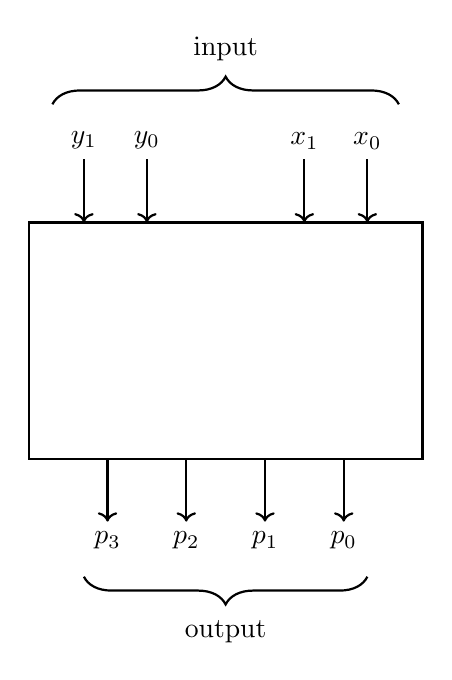
\begin{tikzpicture}
        
        % Main Box
        \draw[thick] (-2.5, -1.5) rectangle (2.5, 1.5);
        
        % Input Arrows and Labels
        \draw[->, thick] (-1.8, 2.3) node[above] {$y_1$} -- (-1.8, 1.5);
        \draw[->, thick] (-1.0, 2.3) node[above] {$y_0$} -- (-1.0, 1.5);
        \draw[->, thick] (1.0, 2.3) node[above] {$x_1$} -- (1.0, 1.5);
        \draw[->, thick] (1.8, 2.3) node[above] {$x_0$} -- (1.8, 1.5);
        
        % Top Curly Brace for "input"
        \draw[decorate, decoration={brace, amplitude=10pt}, thick] 
            (-2.2, 3) -- (2.2, 3) node[midway, above=12pt] {input};

        % Output Arrows and Labels
        \draw[->, thick] (-1.5, -1.5) -- (-1.5, -2.3) node[below] {$p_3$};
        \draw[->, thick] (-0.5, -1.5) -- (-0.5, -2.3) node[below] {$p_2$};
        \draw[->, thick] (0.5, -1.5) -- (0.5, -2.3) node[below] {$p_1$};
        \draw[->, thick] (1.5, -1.5) -- (1.5, -2.3) node[below] {$p_0$};
        
        % Bottom Curly Brace for "output"
        \draw[decorate, decoration={brace, amplitude=10pt, mirror}, thick] 
            (-1.8, -3) -- (1.8, -3) node[midway, below=12pt] {output};
            
    \end{tikzpicture}
\end{center}

\begin{tcolorbox}[enhanced,breakable,ansbox,colback=cD!4,colframe=cD,boxrule=0.8pt,arc=5pt,title={\textbf{Answer}},fonttitle=\bfseries\color{white},colbacktitle=cD]

\subsubsection*{1. Mathematical Formulation of the $2 \times 2$ Multiplier}

Let the two 2-bit input variables be the Multiplicand $X = x_1 x_0$ and the Multiplier $Y = y_1 y_0$. The maximum value for each input is $3_{10}$ ($11_2$), meaning the maximum possible product is $3 \times 3 = 9_{10}$ ($1001_2$). Thus, the final product requires 4 bits: $P = p_3 p_2 p_1 p_0$.

The multiplication is performed by generating partial products using logical AND operations and summing them based on their binary positional weights.

\begin{center}
\renewcommand{\arraystretch}{1.2}
\begin{tabular}{ccccc}
  &   &   & $x_1$ & $x_0$ \\
$\times$ &   &   & $y_1$ & $y_0$ \\
\toprule
  &   &   & $x_1 y_0$ & $x_0 y_0$  \\
+ &   & $x_1 y_1$ & $x_0 y_1$ &   \\
\midrule
  & $p_3$ & $p_2$ & $p_1$ & $p_0$ \\
\bottomrule
\end{tabular}
\end{center}

\subsubsection*{2. Boolean Logic Equations}

From the positional addition in the table above, we can derive the boolean expressions for each bit of the product:

\begin{itemize}
    \item \textbf{Bit $p_0$ (Weight $2^0$):} This is exactly the first partial product.
    \begin{align*}
        \textcolor{cD}{p_0 = x_0 \cdot y_0}
    \end{align*}
    
    \item \textbf{Bit $p_1$ (Weight $2^1$):} This is the sum of $x_1 y_0$ and $x_0 y_1$. We can use a \textbf{Half Adder (HA1)} for this addition.
    \begin{align*}
        \textcolor{cD}{p_1 = (x_1 \cdot y_0) \oplus (x_0 \cdot y_1)} \quad &\text{(Sum from HA1)} \\
        c_1 = (x_1 \cdot y_0) \cdot (x_0 \cdot y_1) \quad &\text{(Carry from HA1)}
    \end{align*}
    
    \item \textbf{Bits $p_2$ and $p_3$ (Weights $2^2$ and $2^3$):} $p_2$ is the sum of the partial product $x_1 y_1$ and the carry $c_1$ from the previous column. This requires a second \textbf{Half Adder (HA2)}. The carry from this addition forms the most significant bit, $p_3$.
    \begin{align*}
        \textcolor{cD}{p_2 = (x_1 \cdot y_1) \oplus c_1} \quad &\text{(Sum from HA2)} \\
        \textcolor{cD}{p_3 = (x_1 \cdot y_1) \cdot c_1} \quad &\text{(Carry from HA2)}
    \end{align*}
\end{itemize}

\subsubsection*{3. Gate-Level Circuit Diagram}

The circuit is constructed using four 2-input AND gates to generate the partial products, and two Half Adders (each consisting of an XOR gate and an AND gate) to perform the summation.

\vspace{0.5cm}
\begin{center}
\begin{circuitikz}[scale=0.9, transform shape]
    
    % Input lines
    \node[above, font=\bfseries] at (0, 1) {$x_1$};
    \node[above, font=\bfseries] at (1, 1) {$x_0$};
    \node[above, font=\bfseries] at (2, 1) {$y_1$};
    \node[above, font=\bfseries] at (3, 1) {$y_0$};
    
    \draw (0,1) -- (0,-9);
    \draw (1,1) -- (1,-9);
    \draw (2,1) -- (2,-9);
    \draw (3,1) -- (3,-9);

    % Partial Product AND Gates
    \node[and port] (a00) at (6, 0) {};
    \node[and port] (a10) at (6, -2) {};
    \node[and port] (a01) at (6, -4) {};
    \node[and port] (a11) at (6, -7) {};
    
    % Connections for x0 y0
    \draw (1, 0.28) node[circle, fill, inner sep=1pt]{} -- (a00.in 1);
    \draw (3, -0.28) node[circle, fill, inner sep=1pt]{} -- (a00.in 2);
    
    % Connections for x1 y0
    \draw (0, -1.72) node[circle, fill, inner sep=1pt]{} -- (a10.in 1);
    \draw (3, -2.28) node[circle, fill, inner sep=1pt]{} -- (a10.in 2);
    
    % Connections for x0 y1
    \draw (1, -3.72) node[circle, fill, inner sep=1pt]{} -- (a01.in 1);
    \draw (2, -4.28) node[circle, fill, inner sep=1pt]{} -- (a01.in 2);
    
    % Connections for x1 y1
    \draw (0, -6.72) node[circle, fill, inner sep=1pt]{} -- (a11.in 1);
    \draw (2, -7.28) node[circle, fill, inner sep=1pt]{} -- (a11.in 2);

    % Output p0
    \draw[thick] (a00.out) -- ++(7,0) node[right, font=\bfseries, text=cD] {$p_0$};

    % Half Adder 1 (for p1 and c1)
    \node[xor port] (x1) at (9, -3) {};
    \node[and port] (c1) at (9, -5) {};
    
    \draw (a10.out) -- ++(0.5,0) coordinate (fork1);
    \draw (fork1) |- (x1.in 1);
    \draw (fork1) node[circle, fill, inner sep=1pt]{} |- (c1.in 1);
    
    \draw (a01.out) -- ++(0.8,0) coordinate (fork2);
    \draw (fork2) |- (x1.in 2);
    \draw (fork2) node[circle, fill, inner sep=1pt]{} |- (c1.in 2);

    % Output p1
    \draw[thick] (x1.out) -- ++(4,0) node[right, font=\bfseries, text=cD] {$p_1$};

    % Half Adder 2 (for p2 and p3)
    \node[xor port] (x2) at (12, -6) {};
    \node[and port] (c2) at (12, -8) {};
    
    \draw (a11.out) -- ++(2.5,0) coordinate (fork3);
    \draw (fork3) |- (x2.in 1);
    \draw (fork3) node[circle, fill, inner sep=1pt]{} |- (c2.in 1);
    
    \draw (c1.out) -- ++(0.5,0) coordinate (fork4);
    \draw (fork4) |- (x2.in 2);
    \draw (fork4) node[circle, fill, inner sep=1pt]{} |- (c2.in 2);

    % Outputs p2 and p3
    \draw[thick] (x2.out) -- ++(1,0) node[right, font=\bfseries, text=cD] {$p_2$};
    \draw[thick] (c2.out) -- ++(1,0) node[right, font=\bfseries, text=cD] {$p_3$};
    
    % Grouping labels for Half Adders
    \draw[dashed, rounded corners=3pt, draw=gray] (7.5, -2) rectangle (10.5, -5.8);
    \node[text=gray, font=\footnotesize] at (9, -5.5) {Half Adder 1};
    
    \draw[dashed, rounded corners=3pt, draw=gray] (10.6, -5) rectangle (13.5, -8.8);
    \node[text=gray, font=\footnotesize] at (12, -8.5) {Half Adder 2};

\end{circuitikz}
\end{center}

\end{tcolorbox}

\end{enumerate}

%%──────────────────────────────────────────────────────────────────────
\subtopic{cD}{Incrementer}
\label{sub:s4-incrementer}

\begin{enumerate}


\item Design a 4-bit combinational circuit incrementer (a circuit that adds 1 to a 4-bit binary number) using only half adders.
\mk{10} \yr{CSE 205 | L-2/T-1 | 2021--22}

\begin{tcolorbox}[enhanced,breakable,ansbox,colback=cD!4,colframe=cD,boxrule=0.8pt,arc=5pt,title={\textbf{Answer}},fonttitle=\bfseries\color{white},colbacktitle=cD]

\subsection*{1. Mathematical Derivation of the Incrementer}

An incrementer is a combinational circuit that adds a constant $1$ to a given binary number. Let the 4-bit input be $A = A_3 A_2 A_1 A_0$. We are performing the arithmetic addition:
\[ A + 0001_2 \]

In a standard addition process, each bit position $i$ uses a Full Adder with inputs $A_i$, $B_i$, and $C_i$ (Carry-in). A Full Adder performs the following operations:
\begin{align*}
    S_i &= A_i \oplus B_i \oplus C_i \\
    C_{i+1} &= (A_i \cdot B_i) + C_i \cdot (A_i \oplus B_i)
\end{align*}

Let us evaluate this for our specific addition where the second operand $B = 0001_2$. 

\subsubsection*{Stage 0 (Least Significant Bit)}
For the LSB ($i=0$), we are adding $A_0$ and $B_0 = 1$. The initial carry-in $C_0 = 0$.
\begin{align*}
    S_0 &= A_0 \oplus 1 \oplus 0 = A_0 \oplus 1 \quad &\text{(Equivalent to $\overline{A_0}$)} \\
    C_1 &= (A_0 \cdot 1) + 0 \cdot (A_0 \oplus 1) = A_0 \cdot 1
\end{align*}
These equations, $S_0 = A_0 \oplus 1$ and $C_1 = A_0 \cdot 1$, perfectly match the boolean expressions for a \textbf{Half Adder} where the two inputs are $A_0$ and $1$.

\subsubsection*{Stages 1, 2, and 3 (Higher-Order Bits)}
For the remaining bits ($i = 1, 2, 3$), the bit from the second operand is always $B_i = 0$. Substituting $B_i = 0$ into the Full Adder equations yields:
\begin{align*}
    S_i &= A_i \oplus 0 \oplus C_i = A_i \oplus C_i \\
    C_{i+1} &= (A_i \cdot 0) + C_i \cdot (A_i \oplus 0) = A_i \cdot C_i
\end{align*}
Notice that these reduced equations, $S_i = A_i \oplus C_i$ and $C_{i+1} = A_i \cdot C_i$, are functionally identical to a \textbf{Half Adder} where the two inputs are $A_i$ and $C_i$.

\vspace{0.2cm}
\begin{center}
    \textbf{Conclusion:} Because one of the operands is fixed to zero for all positions except the LSB, every Full Adder stage degrades gracefully into a Half Adder stage. Therefore, a 4-bit incrementer can be implemented using exactly four cascaded Half Adders.
\end{center}

\subsection*{2. Logic Circuit Diagram}

The circuit routes the incoming carry from the previous Half Adder directly into the next Half Adder. The LSB Half Adder receives a constant Logic High ($1$) as its secondary input.

\vspace{0.6cm}
\begin{center}
\begin{circuitikz}[scale=1, transform shape]
    % Define Half Adder block style
    \tikzset{ha/.style={draw=cD, thick, rectangle, minimum height=2.2cm, minimum width=1.6cm, fill=white, rounded corners=3pt, font=\large\bfseries}}

    % Instantiate 4 Half Adders
    \node[ha] (HA0) at (9,0) {HA};
    \node[ha] (HA1) at (6,0) {HA};
    \node[ha] (HA2) at (3,0) {HA};
    \node[ha] (HA3) at (0,0) {HA};

    % Add internal port labels to each HA block
    \foreach \i in {0,1,2,3} {
        \node[below, font=\scriptsize, text=gray] at (HA\i.north) {In};
        \node[left, font=\scriptsize, text=gray] at (HA\i.east) {In};
        \node[above, font=\scriptsize, text=gray] at (HA\i.south) {Sum};
        \node[right, font=\scriptsize, text=gray] at (HA\i.west) {$C_{out}$};
    }

    % HA0 Connections (LSB)
    \draw[thick] (9,2.5) node[above, font=\bfseries] {$A_0$} -- (HA0.north);
    \draw[thick] (11,0) node[right, font=\bfseries] {Logic $1$} -- (HA0.east);
    \draw[thick] (HA0.south) -- (9,-2.5) node[below, font=\bfseries, text=cD, scale=1.2] {$S_0$};
    \draw[thick, text=cD] (HA0.west) -- (HA1.east) node[midway, above, font=\footnotesize, text=black] {$C_1$};

    % HA1 Connections
    \draw[thick] (6,2.5) node[above, font=\bfseries] {$A_1$} -- (HA1.north);
    \draw[thick] (HA1.south) -- (6,-2.5) node[below, font=\bfseries, text=cD, scale=1.2] {$S_1$};
    \draw[thick, text=cD] (HA1.west) -- (HA2.east) node[midway, above, font=\footnotesize, text=black] {$C_2$};

    % HA2 Connections
    \draw[thick] (3,2.5) node[above, font=\bfseries] {$A_2$} -- (HA2.north);
    \draw[thick] (HA2.south) -- (3,-2.5) node[below, font=\bfseries, text=cD, scale=1.2] {$S_2$};
    \draw[thick, text=cD] (HA2.west) -- (HA3.east) node[midway, above, font=\footnotesize, text=black] {$C_3$};

    % HA3 Connections (MSB)
    \draw[thick] (0,2.5) node[above, font=\bfseries] {$A_3$} -- (HA3.north);
    \draw[thick] (HA3.south) -- (0,-2.5) node[below, font=\bfseries, text=cD, scale=1.2] {$S_3$};
    \draw[thick, text=cD] (HA3.west) -- (-2,0) node[left, font=\bfseries, text=cD, scale=1.2] {$C_{out}$};

\end{circuitikz}
\end{center}

\end{tcolorbox}

\item Design a 4-bit incrementer circuit using 4 half-adders. Note that the incrementer circuit adds 1 to a binary number.
\mk{10} \yr{CSE 205 | L-2/T-1 | 2011--12}

\begin{tcolorbox}[enhanced,breakable,ansbox,colback=cD!4,colframe=cD,boxrule=0.8pt,arc=5pt,title={\textbf{Answer}},fonttitle=\bfseries\color{white},colbacktitle=cD]

\subsection*{1. Mathematical Derivation of the Incrementer}

An incrementer circuit adds a constant value of $1$ to a given binary number. Let the 4-bit input number be represented as $A = A_3 A_2 A_1 A_0$. We wish to perform the arithmetic operation:
\[ A + 0001_2 \]

In a general binary addition, each bit position $i$ utilizes a Full Adder with inputs $A_i$, $B_i$, and $C_i$ (Carry-in). A Full Adder performs:
\begin{align*}
    S_i &= A_i \oplus B_i \oplus C_i \\
    C_{i+1} &= (A_i \cdot B_i) + C_i \cdot (A_i \oplus B_i)
\end{align*}

Let us evaluate these equations for our specific increment operation, where the second operand is $B = 0001_2$. 

\subsubsection*{Stage 0 (Least Significant Bit)}
For the LSB ($i=0$), we are adding $A_0$ and $B_0 = 1$. The initial carry-in to the circuit is $C_0 = 0$.
\begin{align*}
    S_0 &= A_0 \oplus 1 \oplus 0 = A_0 \oplus 1 \quad &\text{(Equivalent to $\overline{A_0}$)} \\
    C_1 &= (A_0 \cdot 1) + 0 \cdot (A_0 \oplus 1) = A_0 \cdot 1
\end{align*}
These expressions, $S_0 = A_0 \oplus 1$ and $C_1 = A_0 \cdot 1$, precisely define a \textbf{Half Adder} whose two inputs are $A_0$ and a constant logic $1$.

\subsubsection*{Stages 1, 2, and 3 (Higher-Order Bits)}
For all remaining bits ($i = 1, 2, 3$), the bit from the second operand is zero ($B_i = 0$). Substituting $B_i = 0$ into the Full Adder equations yields:
\begin{align*}
    S_i &= A_i \oplus 0 \oplus C_i = A_i \oplus C_i \\
    C_{i+1} &= (A_i \cdot 0) + C_i \cdot (A_i \oplus 0) = A_i \cdot C_i
\end{align*}
Notice that these reduced equations, $S_i = A_i \oplus C_i$ and $C_{i+1} = A_i \cdot C_i$, are functionally identical to a \textbf{Half Adder} where the two inputs are $A_i$ and the carry $C_i$ from the preceding stage.

\vspace{0.2cm}
\begin{center}
    \textbf{Conclusion:} Since the operand added is fixed to zero for all positions except the LSB, every Full Adder stage reduces to a Half Adder. Thus, a 4-bit incrementer can be elegantly implemented using a cascade of exactly four Half Adders.
\end{center}

\subsection*{2. Logic Circuit Diagram}

The circuit diagram below illustrates the implementation. The incoming carry from the previous Half Adder is routed directly into one of the inputs of the next Half Adder. The LSB Half Adder receives a constant Logic High ($1$) as its secondary input to inject the $+1$ value.

\vspace{0.6cm}
\begin{center}
\begin{circuitikz}[scale=1, transform shape]
    % Define Half Adder block style
    \tikzset{ha/.style={draw=cD, thick, rectangle, minimum height=2.2cm, minimum width=1.6cm, fill=white, rounded corners=3pt, font=\large\bfseries}}

    % Instantiate 4 Half Adders (Right to Left for standard binary weighting)
    \node[ha] (HA0) at (9,0) {HA};
    \node[ha] (HA1) at (6,0) {HA};
    \node[ha] (HA2) at (3,0) {HA};
    \node[ha] (HA3) at (0,0) {HA};

    % Add internal port labels to each HA block
    \foreach \i in {0,1,2,3} {
        \node[below, font=\scriptsize, text=gray] at (HA\i.north) {In};
        \node[left, font=\scriptsize, text=gray] at (HA\i.east) {In};
        \node[above, font=\scriptsize, text=gray] at (HA\i.south) {Sum};
        \node[right, font=\scriptsize, text=gray] at (HA\i.west) {$C_{out}$};
    }

    % HA0 Connections (LSB)
    \draw[thick] (9,2.5) node[above, font=\bfseries] {$A_0$} -- (HA0.north);
    \draw[thick] (11,0) node[right, font=\bfseries] {Logic $1$} -- (HA0.east);
    \draw[thick] (HA0.south) -- (9,-2.5) node[below, font=\bfseries, text=cD, scale=1.2] {$S_0$};
    \draw[thick, text=cD] (HA0.west) -- (HA1.east) node[midway, above, font=\footnotesize, text=black] {$C_1$};

    % HA1 Connections
    \draw[thick] (6,2.5) node[above, font=\bfseries] {$A_1$} -- (HA1.north);
    \draw[thick] (HA1.south) -- (6,-2.5) node[below, font=\bfseries, text=cD, scale=1.2] {$S_1$};
    \draw[thick, text=cD] (HA1.west) -- (HA2.east) node[midway, above, font=\footnotesize, text=black] {$C_2$};

    % HA2 Connections
    \draw[thick] (3,2.5) node[above, font=\bfseries] {$A_2$} -- (HA2.north);
    \draw[thick] (HA2.south) -- (3,-2.5) node[below, font=\bfseries, text=cD, scale=1.2] {$S_2$};
    \draw[thick, text=cD] (HA2.west) -- (HA3.east) node[midway, above, font=\footnotesize, text=black] {$C_3$};

    % HA3 Connections (MSB)
    \draw[thick] (0,2.5) node[above, font=\bfseries] {$A_3$} -- (HA3.north);
    \draw[thick] (HA3.south) -- (0,-2.5) node[below, font=\bfseries, text=cD, scale=1.2] {$S_3$};
    \draw[thick, text=cD] (HA3.west) -- (-2,0) node[left, font=\bfseries, text=cD, scale=1.2] {$C_{out}$};

\end{circuitikz}
\end{center}

\end{tcolorbox}

\end{enumerate}

%%──────────────────────────────────────────────────────────────────────
\subtopic{cD}{Encoders \& Decoders}
\label{sub:s4-encoders}

\begin{enumerate}

\item Design a light sensor based controller circuit for accessing eight servers A, B, C, D, E, F, G, H. The light sensors are numbered as $S_1, S_2, \ldots$ and so on. The sensors of the controller will be ON to show which server is active. The servers have some priority order: C, A, E, H, D, G, F, B (C has the highest priority and B has the lowest priority).
\mk{15} \yr{CSE 205 | L-2/T-1 | 2024--25}

\begin{tcolorbox}[enhanced,breakable,ansbox,colback=cD!4,colframe=cD,boxrule=0.8pt,arc=5pt,title={\textbf{Answer}},fonttitle=\bfseries\color{white},colbacktitle=cD]

\subsection*{1. System Architecture \& Priority Mapping}

The problem requires a controller that manages access to eight servers based on a strict priority hierarchy and indicates the active server using light sensors. Since multiple servers might request access simultaneously, we must resolve these requests using a \textbf{Priority Encoder}. The encoder will generate a unique binary code for the highest-priority active request. This code is then fed into a \textbf{Decoder}, which activates exactly one output line to turn on the corresponding light sensor.

Let the requests from the servers be $R_C, R_A, R_E, R_H, R_D, R_G, R_F, R_B$. 
We map these to the inputs $D_7$ to $D_0$ of an 8-to-3 Priority Encoder, where $D_7$ has the highest priority and $D_0$ has the lowest. The outputs of the 3-to-8 Decoder ($Y_7$ to $Y_0$) will drive the light sensors $S_1$ to $S_8$.

\begin{center}
\renewcommand{\arraystretch}{1.2}
\begin{tabular}{cclcc}
\toprule
\textbf{Priority} & \textbf{Server} & \textbf{Encoder Input} & \textbf{Decoder Output} & \textbf{Active Sensor} \\
\midrule
7 (Highest) & \textbf{C} & $D_7 = R_C$ & $Y_7$ & $S_1$ \\
6 & \textbf{A} & $D_6 = R_A$ & $Y_6$ & $S_2$ \\
5 & \textbf{E} & $D_5 = R_E$ & $Y_5$ & $S_3$ \\
4 & \textbf{H} & $D_4 = R_H$ & $Y_4$ & $S_4$ \\
3 & \textbf{D} & $D_3 = R_D$ & $Y_3$ & $S_5$ \\
2 & \textbf{G} & $D_2 = R_G$ & $Y_2$ & $S_6$ \\
1 & \textbf{F} & $D_1 = R_F$ & $Y_1$ & $S_7$ \\
0 (Lowest)  & \textbf{B} & $D_0 = R_B$ & $Y_0$ & $S_8$ \\
\bottomrule
\end{tabular}
\end{center}

\subsection*{2. Truth Table \& Boolean Equations for the Priority Encoder}

The 8-to-3 Priority Encoder generates a 3-bit binary output $A_2 A_1 A_0$ and a Valid Bit ($V$) which is high ($1$) if at least one request is active. We use 'X' to denote "Don't Care" conditions for lower-priority inputs when a higher-priority input is active.

\begin{center}
\renewcommand{\arraystretch}{1.1}
\resizebox{\textwidth}{!}{
\begin{tabular}{cccccccc|cccc}
\toprule
\multicolumn{8}{c|}{\textbf{Server Requests (Encoder Inputs)}} & \multicolumn{4}{c}{\textbf{Outputs}} \\
$D_7$ (C) & $D_6$ (A) & $D_5$ (E) & $D_4$ (H) & $D_3$ (D) & $D_2$ (G) & $D_1$ (F) & $D_0$ (B) & $A_2$ & $A_1$ & $A_0$ & $V$ (Enable) \\
\midrule
0 & 0 & 0 & 0 & 0 & 0 & 0 & 0 & 0 & 0 & 0 & \textcolor{cD}{\textbf{0}} \\
1 & X & X & X & X & X & X & X & 1 & 1 & 1 & \textcolor{cD}{\textbf{1}} \\
0 & 1 & X & X & X & X & X & X & 1 & 1 & 0 & \textcolor{cD}{\textbf{1}} \\
0 & 0 & 1 & X & X & X & X & X & 1 & 0 & 1 & \textcolor{cD}{\textbf{1}} \\
0 & 0 & 0 & 1 & X & X & X & X & 1 & 0 & 0 & \textcolor{cD}{\textbf{1}} \\
0 & 0 & 0 & 0 & 1 & X & X & X & 0 & 1 & 1 & \textcolor{cD}{\textbf{1}} \\
0 & 0 & 0 & 0 & 0 & 1 & X & X & 0 & 1 & 0 & \textcolor{cD}{\textbf{1}} \\
0 & 0 & 0 & 0 & 0 & 0 & 1 & X & 0 & 0 & 1 & \textcolor{cD}{\textbf{1}} \\
0 & 0 & 0 & 0 & 0 & 0 & 0 & 1 & 0 & 0 & 0 & \textcolor{cD}{\textbf{1}} \\
\bottomrule
\end{tabular}}
\end{center}

Using Boolean algebra, we can extract the Sum-of-Products (SOP) expressions for the encoder outputs. A specific output bit is high if the highest active priority input corresponds to a '1' in that bit's binary weight:
\begin{align*}
    V &= D_7 + D_6 + D_5 + D_4 + D_3 + D_2 + D_1 + D_0 \\
    A_2 &= D_7 + D_6 + D_5 + D_4 \\
    A_1 &= D_7 + D_6 + \overline{D_5} \cdot \overline{D_4} \cdot D_3 + \overline{D_5} \cdot \overline{D_4} \cdot D_2 \\
    A_0 &= D_7 + \overline{D_6} \cdot D_5 + \overline{D_6} \cdot \overline{D_4} \cdot D_3 + \overline{D_6} \cdot \overline{D_4} \cdot \overline{D_2} \cdot D_1
\end{align*}

\subsection*{3. Controller Logic Circuit Diagram}

The controller is implemented using Medium Scale Integration (MSI) blocks. The Valid Bit ($V$) from the Priority Encoder acts as the Enable ($E$) pin for the 3-to-8 Decoder. This ensures that no light sensor turns on if no server is requested.

\vspace{0.6cm}
\begin{center}
\begin{circuitikz}[scale=0.9, transform shape]
    
    % Priority Encoder Block
    \node[draw=cD, thick, rectangle, minimum height=8cm, minimum width=3.5cm, fill=white, rounded corners=3pt, align=center] (PE) at (0,0) {\Large \textbf{8-to-3} \\ \Large \textbf{Priority} \\ \Large \textbf{Encoder}};
    
    % Decoder Block
    \node[draw=cD, thick, rectangle, minimum height=8cm, minimum width=3.5cm, fill=white, rounded corners=3pt, align=center] (DEC) at (8,0) {\Large \textbf{3-to-8} \\ \Large \textbf{Decoder}};

    % Inputs to Priority Encoder
    \draw[thick] (-3, 3.5) node[left] {$R_C$ (Priority 7)} -- ([yshift=3.5cm]PE.west) node[right, font=\bfseries] {$D_7$};
    \draw[thick] (-3, 2.5) node[left] {$R_A$ (Priority 6)} -- ([yshift=2.5cm]PE.west) node[right, font=\bfseries] {$D_6$};
    \draw[thick] (-3, 1.5) node[left] {$R_E$ (Priority 5)} -- ([yshift=1.5cm]PE.west) node[right, font=\bfseries] {$D_5$};
    \draw[thick] (-3, 0.5) node[left] {$R_H$ (Priority 4)} -- ([yshift=0.5cm]PE.west) node[right, font=\bfseries] {$D_4$};
    \draw[thick] (-3, -0.5) node[left] {$R_D$ (Priority 3)} -- ([yshift=-0.5cm]PE.west) node[right, font=\bfseries] {$D_3$};
    \draw[thick] (-3, -1.5) node[left] {$R_G$ (Priority 2)} -- ([yshift=-1.5cm]PE.west) node[right, font=\bfseries] {$D_2$};
    \draw[thick] (-3, -2.5) node[left] {$R_F$ (Priority 1)} -- ([yshift=-2.5cm]PE.west) node[right, font=\bfseries] {$D_1$};
    \draw[thick] (-3, -3.5) node[left] {$R_B$ (Priority 0)} -- ([yshift=-3.5cm]PE.west) node[right, font=\bfseries] {$D_0$};

    % Connections between Encoder and Decoder
    \draw[thick, text=cD] ([yshift=1.5cm]PE.east) node[left, font=\bfseries, text=black] {$A_2$} -- ([yshift=1.5cm]DEC.west) node[right, font=\bfseries, text=black] {$A_2$};
    \draw[thick, text=cD] ([yshift=0cm]PE.east) node[left, font=\bfseries, text=black] {$A_1$} -- ([yshift=0cm]DEC.west) node[right, font=\bfseries, text=black] {$A_1$};
    \draw[thick, text=cD] ([yshift=-1.5cm]PE.east) node[left, font=\bfseries, text=black] {$A_0$} -- ([yshift=-1.5cm]DEC.west) node[right, font=\bfseries, text=black] {$A_0$};
    
    % Valid bit to Enable pin
    \draw[thick, dashed, text=cD] ([yshift=-3.5cm]PE.east) node[left, font=\bfseries, text=black] {$V$} -- ([yshift=-3.5cm]DEC.west) node[right, font=\bfseries, text=black] {$E$};
    \node[above, font=\footnotesize, text=gray] at (4, -3.5) {Enable active when $V=1$};

    % Outputs from Decoder
    \draw[thick] ([yshift=3.5cm]DEC.east) node[left, font=\bfseries] {$Y_7$} -- (11, 3.5) node[right, text=cD, font=\bfseries] {$S_1$ (Server C ON)};
    \draw[thick] ([yshift=2.5cm]DEC.east) node[left, font=\bfseries] {$Y_6$} -- (11, 2.5) node[right, text=cD, font=\bfseries] {$S_2$ (Server A ON)};
    \draw[thick] ([yshift=1.5cm]DEC.east) node[left, font=\bfseries] {$Y_5$} -- (11, 1.5) node[right, text=cD, font=\bfseries] {$S_3$ (Server E ON)};
    \draw[thick] ([yshift=0.5cm]DEC.east) node[left, font=\bfseries] {$Y_4$} -- (11, 0.5) node[right, text=cD, font=\bfseries] {$S_4$ (Server H ON)};
    \draw[thick] ([yshift=-0.5cm]DEC.east) node[left, font=\bfseries] {$Y_3$} -- (11, -0.5) node[right, text=cD, font=\bfseries] {$S_5$ (Server D ON)};
    \draw[thick] ([yshift=-1.5cm]DEC.east) node[left, font=\bfseries] {$Y_2$} -- (11, -1.5) node[right, text=cD, font=\bfseries] {$S_6$ (Server G ON)};
    \draw[thick] ([yshift=-2.5cm]DEC.east) node[left, font=\bfseries] {$Y_1$} -- (11, -2.5) node[right, text=cD, font=\bfseries] {$S_7$ (Server F ON)};
    \draw[thick] ([yshift=-3.5cm]DEC.east) node[left, font=\bfseries] {$Y_0$} -- (11, -3.5) node[right, text=cD, font=\bfseries] {$S_8$ (Server B ON)};

\end{circuitikz}
\end{center}

\end{tcolorbox}

\item Show the truth table of an 8-to-3 line priority encoder, where higher priority is given to lower numbered input.
\mk{9} \yr{CSE 205 | L-2/T-1 | 2023--24}

\begin{tcolorbox}[enhanced,breakable,ansbox,colback=cD!4,colframe=cD,boxrule=0.8pt,arc=5pt,title={\textbf{Answer}},fonttitle=\bfseries\color{white},colbacktitle=cD]

\subsection*{1. Problem Analysis and Priority Definition}

An 8-to-3 line priority encoder compresses eight inputs ($D_0$ to $D_7$) into a 3-bit binary output ($A_2, A_1, A_0$). It also typically includes a Valid output bit ($V$) to distinguish between the state where input $D_0$ is active versus the state where no inputs are active.

In a standard priority encoder, higher-numbered inputs usually have higher priority. However, this specific problem dictates a \textbf{reversed priority scheme}: \textbf{the lower-numbered input has the higher priority}. 
\begin{itemize}
    \item \textbf{Highest Priority:} $D_0$
    \item \textbf{Lowest Priority:} $D_7$
\end{itemize}

This implies that if $D_0$ is active ($1$), the encoder will output the binary equivalent of $0$ ($000_2$), completely ignoring the states of all other inputs $D_1$ through $D_7$. The system only considers $D_1$ if $D_0 = 0$, and so on.

\subsection*{2. Truth Table Construction}

In the table below, 'X' represents a \textbf{Don't Care} condition, meaning the input can be either $0$ or $1$ without affecting the output, due to a higher-priority input already dictating the result.

\vspace{0.4cm}
\begin{center}
\resizebox{0.95\textwidth}{!}{
\begin{tabular}{cccccccc|cccc}
\toprule
\multicolumn{8}{c|}{\textbf{Inputs (Highest to Lowest Priority)}} & \multicolumn{4}{c}{\textbf{Outputs}} \\
$D_0$ & $D_1$ & $D_2$ & $D_3$ & $D_4$ & $D_5$ & $D_6$ & $D_7$ & $A_2$ & $A_1$ & $A_0$ & \textbf{Valid ($V$)} \\
\midrule
0 & 0 & 0 & 0 & 0 & 0 & 0 & 0 & 0 & 0 & 0 & \textcolor{cD}{\textbf{0}} \\
1 & X & X & X & X & X & X & X & 0 & 0 & 0 & \textcolor{cD}{\textbf{1}} \\
0 & 1 & X & X & X & X & X & X & 0 & 0 & 1 & \textcolor{cD}{\textbf{1}} \\
0 & 0 & 1 & X & X & X & X & X & 0 & 1 & 0 & \textcolor{cD}{\textbf{1}} \\
0 & 0 & 0 & 1 & X & X & X & X & 0 & 1 & 1 & \textcolor{cD}{\textbf{1}} \\
0 & 0 & 0 & 0 & 1 & X & X & X & 1 & 0 & 0 & \textcolor{cD}{\textbf{1}} \\
0 & 0 & 0 & 0 & 0 & 1 & X & X & 1 & 0 & 1 & \textcolor{cD}{\textbf{1}} \\
0 & 0 & 0 & 0 & 0 & 0 & 1 & X & 1 & 1 & 0 & \textcolor{cD}{\textbf{1}} \\
0 & 0 & 0 & 0 & 0 & 0 & 0 & 1 & 1 & 1 & 1 & \textcolor{cD}{\textbf{1}} \\
\bottomrule
\end{tabular}
}
\end{center}
\vspace{0.2cm}

\subsection*{3. Boolean Output Equations (For Reference)}
Although not strictly asked, defining the Boolean equations based on the truth table demonstrates a complete understanding of the circuit's underlying logic. The outputs are only valid when $V=1$.
\begin{align*}
    V   &= D_0 + D_1 + D_2 + D_3 + D_4 + D_5 + D_6 + D_7 \\
    A_2 &= \overline{D_0} \cdot \overline{D_1} \cdot \overline{D_2} \cdot \overline{D_3} \cdot (D_4 + D_5 + D_6 + D_7) \\
    A_1 &= \overline{D_0} \cdot \overline{D_1} \cdot (D_2 + D_3) + \overline{D_0} \cdot \overline{D_1} \cdot \overline{D_2} \cdot \overline{D_3} \cdot \overline{D_4} \cdot \overline{D_5} \cdot (D_6 + D_7) \\
    A_0 &= \overline{D_0} \cdot D_1 + \overline{D_0} \cdot \overline{D_1} \cdot \overline{D_2} \cdot D_3 + \overline{D_0} \cdot \overline{D_1} \cdot \overline{D_2} \cdot \overline{D_3} \cdot \overline{D_4} \cdot D_5 + \overline{D_0} \cdot \overline{D_1} \cdot \overline{D_2} \cdot \overline{D_3} \cdot \overline{D_4} \cdot \overline{D_5} \cdot \overline{D_6} \cdot D_7
\end{align*}

\end{tcolorbox}

\item After a school final result, Ishrat applied for college admission and gave her choices from eight colleges indexed A to H, following the priority order B, A, D, E, F, H, G, C (B has the highest priority, C has the lowest priority). Find the Boolean function of her choices and show the design steps.
\mk{15} \yr{CSE 205 | L-2/T-1 | 2020--21}

\begin{tcolorbox}[enhanced,breakable,ansbox,colback=cD!4,colframe=cD,boxrule=0.8pt,arc=5pt,title={\textbf{Answer}},fonttitle=\bfseries\color{white},colbacktitle=cD]

\subsection*{1. Problem Definition and Priority Mapping}

The problem describes a system where eight choices (colleges A through H) are ranked by priority. The system must output a unique binary code corresponding to the highest-priority college chosen. This requires an \textbf{8-to-3 Priority Encoder}. 

First, we assign priority levels $7$ (highest) down to $0$ (lowest) and map each college to an input variable $I_7 \dots I_0$:

\begin{center}
\renewcommand{\arraystretch}{1.2}
\begin{tabular}{llccc}
\toprule
\textbf{Priority} & \textbf{College} & \textbf{Input Var} & \textbf{Output Code ($Y_2 Y_1 Y_0$)} \\
\midrule
7 (Highest) & \textbf{B} & $I_7$ & 1 1 1 \\
6 & \textbf{A} & $I_6$ & 1 1 0 \\
5 & \textbf{D} & $I_5$ & 1 0 1 \\
4 & \textbf{E} & $I_4$ & 1 0 0 \\
3 & \textbf{F} & $I_3$ & 0 1 1 \\
2 & \textbf{H} & $I_2$ & 0 1 0 \\
1 & \textbf{G} & $I_1$ & 0 0 1 \\
0 (Lowest)  & \textbf{C} & $I_0$ & 0 0 0 \\
\bottomrule
\end{tabular}
\end{center}

\subsection*{2. Truth Table Construction}

A valid bit ($V$) is introduced to differentiate the condition where college C ($000$) is chosen from the condition where \textit{no} college is chosen. In the table below, 'X' denotes a "Don't Care" condition, meaning lower priority inputs are ignored when a higher priority input is active.

\begin{center}
\renewcommand{\arraystretch}{1.15}
\resizebox{0.95\textwidth}{!}{
\begin{tabular}{cccccccc|cccc}
\toprule
\multicolumn{8}{c|}{\textbf{College Inputs (Highest to Lowest Priority)}} & \multicolumn{4}{c}{\textbf{Binary Output}} \\
\textbf{B} ($I_7$) & \textbf{A} ($I_6$) & \textbf{D} ($I_5$) & \textbf{E} ($I_4$) & \textbf{F} ($I_3$) & \textbf{H} ($I_2$) & \textbf{G} ($I_1$) & \textbf{C} ($I_0$) & $Y_2$ & $Y_1$ & $Y_0$ & $V$ \\
\midrule
0 & 0 & 0 & 0 & 0 & 0 & 0 & 0 & 0 & 0 & 0 & \textcolor{cD}{\textbf{0}} \\
1 & X & X & X & X & X & X & X & 1 & 1 & 1 & \textcolor{cD}{\textbf{1}} \\
0 & 1 & X & X & X & X & X & X & 1 & 1 & 0 & \textcolor{cD}{\textbf{1}} \\
0 & 0 & 1 & X & X & X & X & X & 1 & 0 & 1 & \textcolor{cD}{\textbf{1}} \\
0 & 0 & 0 & 1 & X & X & X & X & 1 & 0 & 0 & \textcolor{cD}{\textbf{1}} \\
0 & 0 & 0 & 0 & 1 & X & X & X & 0 & 1 & 1 & \textcolor{cD}{\textbf{1}} \\
0 & 0 & 0 & 0 & 0 & 1 & X & X & 0 & 1 & 0 & \textcolor{cD}{\textbf{1}} \\
0 & 0 & 0 & 0 & 0 & 0 & 1 & X & 0 & 0 & 1 & \textcolor{cD}{\textbf{1}} \\
0 & 0 & 0 & 0 & 0 & 0 & 0 & 1 & 0 & 0 & 0 & \textcolor{cD}{\textbf{1}} \\
\bottomrule
\end{tabular}}
\end{center}

\subsection*{3. Boolean Function Derivation}

From the truth table, we derive the Boolean expressions. A specific output bit is high if the highest active priority input possesses a logic '1' in its corresponding binary weight. Lower priority inputs are masked by negating the higher priority inputs. 

\textbf{1. Valid Bit ($V$):} Active if any college is selected.
\begin{align*}
    \textcolor{cD}{V = B + A + D + E + F + H + G + C}
\end{align*}

\textbf{2. Most Significant Bit ($Y_2$):} High for $I_7, I_6, I_5, I_4$.
\begin{align*}
    Y_2 &= I_7 + \overline{I_7}I_6 + \overline{I_7}\overline{I_6}I_5 + \overline{I_7}\overline{I_6}\overline{I_5}I_4 \\
    &= I_7 + I_6 + I_5 + I_4 \quad \text{(By sequential application of } X + \overline{X}Y = X + Y \text{)} \\
    \textcolor{cD}{Y_2} &\textcolor{cD}{= B + A + D + E}
\end{align*}

\textbf{3. Middle Bit ($Y_1$):} High for $I_7, I_6, I_3, I_2$.
\begin{align*}
    Y_1 &= I_7 + \overline{I_7}I_6 + \overline{I_7}\overline{I_6}\overline{I_5}\overline{I_4}I_3 + \overline{I_7}\overline{I_6}\overline{I_5}\overline{I_4}\overline{I_3}I_2 \\
    &= I_7 + I_6 + \overline{I_5}\overline{I_4}I_3 + \overline{I_5}\overline{I_4}I_2 \quad \text{(Absorption of } I_7, I_6 \text{ into subsequent terms)} \\
    \textcolor{cD}{Y_1} &\textcolor{cD}{= B + A + \overline{D}\overline{E}F + \overline{D}\overline{E}H}
\end{align*}

\textbf{4. Least Significant Bit ($Y_0$):} High for $I_7, I_5, I_3, I_1$.
\begin{align*}
    Y_0 &= I_7 + \overline{I_7}\overline{I_6}I_5 + \overline{I_7}\overline{I_6}\overline{I_5}\overline{I_4}I_3 + \overline{I_7}\overline{I_6}\overline{I_5}\overline{I_4}\overline{I_3}\overline{I_2}I_1 \\
    &= I_7 + \overline{I_6}I_5 + \overline{I_6}\overline{I_5}\overline{I_4}I_3 + \overline{I_6}\overline{I_5}\overline{I_4}\overline{I_3}\overline{I_2}I_1 \\
    &= I_7 + \overline{I_6}(I_5 + \overline{I_5}\overline{I_4}I_3) + \dots \\
    &= I_7 + \overline{I_6}I_5 + \overline{I_6}\overline{I_4}I_3 + \overline{I_6}\overline{I_4}\overline{I_2}I_1 \quad \text{(Using Distributive and Boolean logic reductions)} \\
    \textcolor{cD}{Y_0} &\textcolor{cD}{= B + \overline{A}D + \overline{A}\overline{E}F + \overline{A}\overline{E}\overline{H}G}
\end{align*}

\subsection*{4. Logic Circuit Implementation (Block Diagram)}

The derived Boolean functions can be implemented using standard NOT, AND, and OR logic gates. Structurally, they are synthesized inside an 8-to-3 Priority Encoder macro cell.

\vspace{0.4cm}
\begin{center}
\begin{circuitikz}[scale=0.95, transform shape]
    
    % Main Box
    \draw[thick, draw=cD, fill=white, rounded corners=4pt] (0,0) rectangle (6,9);
    \node[align=center, font=\large\bfseries, text=cD] at (3, 4.5) {8-to-3 \\ Priority Encoder \\ \small (Priority Base)};

    % Inputs
    \draw[thick] (-2, 8) node[left] {B (Priority 7)} -- (0, 8) node[right, font=\bfseries] {$I_7$};
    \draw[thick] (-2, 7) node[left] {A (Priority 6)} -- (0, 7) node[right, font=\bfseries] {$I_6$};
    \draw[thick] (-2, 6) node[left] {D (Priority 5)} -- (0, 6) node[right, font=\bfseries] {$I_5$};
    \draw[thick] (-2, 5) node[left] {E (Priority 4)} -- (0, 5) node[right, font=\bfseries] {$I_4$};
    \draw[thick] (-2, 4) node[left] {F (Priority 3)} -- (0, 4) node[right, font=\bfseries] {$I_3$};
    \draw[thick] (-2, 3) node[left] {H (Priority 2)} -- (0, 3) node[right, font=\bfseries] {$I_2$};
    \draw[thick] (-2, 2) node[left] {G (Priority 1)} -- (0, 2) node[right, font=\bfseries] {$I_1$};
    \draw[thick] (-2, 1) node[left] {C (Priority 0)} -- (0, 1) node[right, font=\bfseries] {$I_0$};

    % Outputs
    \draw[thick, text=cD] (6, 7) node[left, font=\bfseries, text=black] {$Y_2$} -- (8, 7) node[right, font=\bfseries] {MSB};
    \draw[thick, text=cD] (6, 5) node[left, font=\bfseries, text=black] {$Y_1$} -- (8, 5) node[right, font=\bfseries] {Bit 1};
    \draw[thick, text=cD] (6, 3) node[left, font=\bfseries, text=black] {$Y_0$} -- (8, 3) node[right, font=\bfseries] {LSB};
    \draw[thick, dashed, text=cD] (6, 1) node[left, font=\bfseries, text=black] {$V$} -- (8, 1) node[right, font=\bfseries] {Valid};

\end{circuitikz}
\end{center}

\end{tcolorbox}

\item Design an 8-to-3 priority encoder with the priority order: 5, 0, 7, 4, 6, 3, 2, 1 (5 has highest priority, 1 has lowest priority).
\mk{13} \yr{CSE 205 | L-2/T-1 | 2018--19}

\begin{tcolorbox}[enhanced,breakable,ansbox,colback=cD!4,colframe=cD,boxrule=0.8pt,arc=5pt,title={\textbf{Answer}},fonttitle=\bfseries\color{white},colbacktitle=cD]

\subsection*{1. Priority Mapping and System Definition}

An 8-to-3 priority encoder takes 8 inputs ($D_0$ to $D_7$) and compresses them into a 3-bit binary output ($Y_2, Y_1, Y_0$) based on a strict priority hierarchy. It also outputs a Valid bit ($V$) to indicate if at least one input is active. 

The problem specifies an irregular priority order. We assign priority levels from 7 (highest) down to 0 (lowest) and map them to their respective inputs and expected binary outputs (the binary index of the active input).

\begin{center}
\renewcommand{\arraystretch}{1.2}
\begin{tabular}{lcccc}
\toprule
\textbf{Priority Level} & \textbf{Input Variable} & \textbf{Active Index} & \textbf{Binary Output ($Y_2 Y_1 Y_0$)} \\
\midrule
7 (Highest) & \textbf{$D_5$} & 5 & 1 0 1 \\
6 & \textbf{$D_0$} & 0 & 0 0 0 \\
5 & \textbf{$D_7$} & 7 & 1 1 1 \\
4 & \textbf{$D_4$} & 4 & 1 0 0 \\
3 & \textbf{$D_6$} & 6 & 1 1 0 \\
2 & \textbf{$D_3$} & 3 & 0 1 1 \\
1 & \textbf{$D_2$} & 2 & 0 1 0 \\
0 (Lowest)  & \textbf{$D_1$} & 1 & 0 0 1 \\
\bottomrule
\end{tabular}
\end{center}

\subsection*{2. Truth Table Construction}

In the truth table, we evaluate the inputs in decreasing order of priority. An 'X' signifies a "Don't Care" condition, indicating that lower-priority inputs are ignored when a higher-priority input is active (Logic 1).

\begin{center}
\renewcommand{\arraystretch}{1.15}
\resizebox{0.95\textwidth}{!}{
\begin{tabular}{cccccccc|cccc}
\toprule
\multicolumn{8}{c|}{\textbf{Inputs (Highest to Lowest Priority)}} & \multicolumn{4}{c}{\textbf{Outputs}} \\
$D_5$ (P7) & $D_0$ (P6) & $D_7$ (P5) & $D_4$ (P4) & $D_6$ (P3) & $D_3$ (P2) & $D_2$ (P1) & $D_1$ (P0) & $Y_2$ & $Y_1$ & $Y_0$ & $V$ \\
\midrule
0 & 0 & 0 & 0 & 0 & 0 & 0 & 0 & 0 & 0 & 0 & \textcolor{cD}{\textbf{0}} \\
1 & X & X & X & X & X & X & X & 1 & 0 & 1 & \textcolor{cD}{\textbf{1}} \\
0 & 1 & X & X & X & X & X & X & 0 & 0 & 0 & \textcolor{cD}{\textbf{1}} \\
0 & 0 & 1 & X & X & X & X & X & 1 & 1 & 1 & \textcolor{cD}{\textbf{1}} \\
0 & 0 & 0 & 1 & X & X & X & X & 1 & 0 & 0 & \textcolor{cD}{\textbf{1}} \\
0 & 0 & 0 & 0 & 1 & X & X & X & 1 & 1 & 0 & \textcolor{cD}{\textbf{1}} \\
0 & 0 & 0 & 0 & 0 & 1 & X & X & 0 & 1 & 1 & \textcolor{cD}{\textbf{1}} \\
0 & 0 & 0 & 0 & 0 & 0 & 1 & X & 0 & 1 & 0 & \textcolor{cD}{\textbf{1}} \\
0 & 0 & 0 & 0 & 0 & 0 & 0 & 1 & 0 & 0 & 1 & \textcolor{cD}{\textbf{1}} \\
\bottomrule
\end{tabular}}
\end{center}

\subsection*{3. Mathematical Derivation of Boolean Equations}

To extract the Boolean expressions, we define mutually exclusive intermediate activation signals ($E_i$) for each input, ensuring it only triggers if all higher-priority inputs are 0.
\begin{align*}
    E_5 &= D_5 \\
    E_0 &= \overline{D_5} \cdot D_0 \\
    E_7 &= \overline{D_5} \cdot \overline{D_0} \cdot D_7 \\
    E_4 &= \overline{D_5} \cdot \overline{D_0} \cdot \overline{D_7} \cdot D_4 \\
    E_6 &= \overline{D_5} \cdot \overline{D_0} \cdot \overline{D_7} \cdot \overline{D_4} \cdot D_6 \\
    E_3 &= \overline{D_5} \cdot \overline{D_0} \cdot \overline{D_7} \cdot \overline{D_4} \cdot \overline{D_6} \cdot D_3 \\
    E_2 &= \overline{D_5} \cdot \overline{D_0} \cdot \overline{D_7} \cdot \overline{D_4} \cdot \overline{D_6} \cdot \overline{D_3} \cdot D_2 \\
    E_1 &= \overline{D_5} \cdot \overline{D_0} \cdot \overline{D_7} \cdot \overline{D_4} \cdot \overline{D_6} \cdot \overline{D_3} \cdot \overline{D_2} \cdot D_1
\end{align*}

The \textbf{Valid Bit ($V$)} is 1 if any input is active:
\begin{align*}
    \textcolor{cD}{V = D_5 + D_0 + D_7 + D_4 + D_6 + D_3 + D_2 + D_1}
\end{align*}

\textbf{Most Significant Bit ($Y_2$):} Active for $D_5$ (101), $D_7$ (111), $D_4$ (100), $D_6$ (110).
\begin{align*}
    Y_2 &= E_5 + E_7 + E_4 + E_6 \\
    &= D_5 + \overline{D_5}\overline{D_0}D_7 + \overline{D_5}\overline{D_0}\overline{D_7}D_4 + \overline{D_5}\overline{D_0}\overline{D_7}\overline{D_4}D_6 \\
    &= D_5 + \overline{D_5}\overline{D_0} \left( D_7 + \overline{D_7}D_4 + \overline{D_7}\overline{D_4}D_6 \right) \quad \text{(Factoring)} \\
    &= D_5 + \overline{D_0} \left( D_7 + D_4 + D_6 \right) \quad \text{(Using Distributive Law: $A + \overline{A}B = A + B$ repeatedly)} \\
    \textcolor{cD}{Y_2} &\textcolor{cD}{= D_5 + \overline{D_0} (D_7 + D_4 + D_6)}
\end{align*}

\textbf{Middle Bit ($Y_1$):} Active for $D_7$ (111), $D_6$ (110), $D_3$ (011), $D_2$ (010).
\begin{align*}
    Y_1 &= E_7 + E_6 + E_3 + E_2 \\
    &= \overline{D_5}\overline{D_0}D_7 + \overline{D_5}\overline{D_0}\overline{D_7}\overline{D_4}D_6 + \overline{D_5}\overline{D_0}\overline{D_7}\overline{D_4}\overline{D_6}D_3 + \overline{D_5}\overline{D_0}\overline{D_7}\overline{D_4}\overline{D_6}\overline{D_3}D_2 \\
    &= \overline{D_5}\overline{D_0} \left( D_7 + \overline{D_7}\overline{D_4}D_6 + \overline{D_7}\overline{D_4}\overline{D_6}D_3 + \overline{D_7}\overline{D_4}\overline{D_6}\overline{D_3}D_2 \right) \\
    &= \overline{D_5}\overline{D_0} \left( D_7 + \overline{D_4} ( D_6 + \overline{D_6}D_3 + \overline{D_6}\overline{D_3}D_2 ) \right) \quad \text{(Applying $A + \overline{A}B = A + B$)} \\
    \textcolor{cD}{Y_1} &\textcolor{cD}{= \overline{D_5}\overline{D_0} (D_7 + \overline{D_4} (D_6 + D_3 + D_2))}
\end{align*}

\textbf{Least Significant Bit ($Y_0$):} Active for $D_5$ (101), $D_7$ (111), $D_3$ (011), $D_1$ (001).
\begin{align*}
    Y_0 &= E_5 + E_7 + E_3 + E_1 \\
    &= D_5 + \overline{D_5}\overline{D_0}D_7 + \overline{D_5}\overline{D_0}\overline{D_7}\overline{D_4}\overline{D_6}D_3 + \overline{D_5}\overline{D_0}\overline{D_7}\overline{D_4}\overline{D_6}\overline{D_3}\overline{D_2}D_1 \\
    &= D_5 + \overline{D_5}\overline{D_0} \left( D_7 + \overline{D_7}\overline{D_4}\overline{D_6}D_3 + \overline{D_7}\overline{D_4}\overline{D_6}\overline{D_3}\overline{D_2}D_1 \right) \\
    &= D_5 + \overline{D_0} \left( D_7 + \overline{D_4}\overline{D_6} ( D_3 + \overline{D_3}\overline{D_2}D_1 ) \right) \quad \text{(Reduction via Distributive Law)} \\
    \textcolor{cD}{Y_0} &\textcolor{cD}{= D_5 + \overline{D_0} (D_7 + \overline{D_4}\overline{D_6}(D_3 + \overline{D_2}D_1))}
\end{align*}

\subsection*{4. Logic Circuit Implementation (Block Diagram)}
The gate-level schematic is constructed directly from the simplified Boolean equations above using AND, OR, and NOT gates. Below is the structural representation of the custom encoder logic block.

\vspace{0.4cm}
\begin{center}
\begin{circuitikz}[scale=0.9, transform shape]
    % Main Box
    \draw[thick, draw=cD, fill=white, rounded corners=5pt] (0,0) rectangle (7,9);
    \node[align=center, font=\Large\bfseries, text=cD] at (3.5, 4.5) {8-to-3 \\ Priority Encoder \\ \large (Custom Sequence)};

    % Inputs mapped by priority
    \draw[thick] (-2.5, 8) node[left] {Priority 7 (Highest)} -- (0, 8) node[right, font=\bfseries] {$D_5$};
    \draw[thick] (-2.5, 7) node[left] {Priority 6} -- (0, 7) node[right, font=\bfseries] {$D_0$};
    \draw[thick] (-2.5, 6) node[left] {Priority 5} -- (0, 6) node[right, font=\bfseries] {$D_7$};
    \draw[thick] (-2.5, 5) node[left] {Priority 4} -- (0, 5) node[right, font=\bfseries] {$D_4$};
    \draw[thick] (-2.5, 4) node[left] {Priority 3} -- (0, 4) node[right, font=\bfseries] {$D_6$};
    \draw[thick] (-2.5, 3) node[left] {Priority 2} -- (0, 3) node[right, font=\bfseries] {$D_3$};
    \draw[thick] (-2.5, 2) node[left] {Priority 1} -- (0, 2) node[right, font=\bfseries] {$D_2$};
    \draw[thick] (-2.5, 1) node[left] {Priority 0 (Lowest)} -- (0, 1) node[right, font=\bfseries] {$D_1$};

    % Outputs
    \draw[thick, text=cD] (7, 7) node[left, font=\bfseries, text=black] {$Y_2$} -- (9, 7) node[right, font=\bfseries] {MSB};
    \draw[thick, text=cD] (7, 5) node[left, font=\bfseries, text=black] {$Y_1$} -- (9, 5) node[right, font=\bfseries] {Bit 1};
    \draw[thick, text=cD] (7, 3) node[left, font=\bfseries, text=black] {$Y_0$} -- (9, 3) node[right, font=\bfseries] {LSB};
    \draw[thick, dashed, text=cD] (7, 1) node[left, font=\bfseries, text=black] {$V$} -- (9, 1) node[right, font=\bfseries] {Valid};

\end{circuitikz}
\end{center}

\end{tcolorbox}

\item Design an 8-to-3 priority encoder with the priority order: 6, 0, 7, 4, 5, 3, 1, 2 (6 has highest priority, 2 has lowest priority).
\mk{13} \yr{CSE 205 | L-2/T-1 | 2017--18}

\begin{tcolorbox}[enhanced,breakable,ansbox,colback=cD!4,colframe=cD,boxrule=0.8pt,arc=5pt,title={\textbf{Answer}},fonttitle=\bfseries\color{white},colbacktitle=cD]

\subsection*{1. System Definition and Priority Mapping}

An 8-to-3 priority encoder compresses eight inputs ($D_0$ through $D_7$) into a 3-bit binary output ($Y_2, Y_1, Y_0$) according to a strict priority hierarchy. It also generates a Valid bit ($V$) to indicate if any input is active. 

The problem specifies an irregular priority order. We assign priority levels from 7 (highest) down to 0 (lowest). The binary output generated corresponds to the numerical index of the highest-priority active input.

\begin{center}
\renewcommand{\arraystretch}{1.2}
\begin{tabular}{lcccc}
\toprule
\textbf{Priority Level} & \textbf{Input Variable} & \textbf{Active Index} & \textbf{Binary Output ($Y_2 Y_1 Y_0$)} \\
\midrule
7 (Highest) & \textbf{$D_6$} & 6 & 1 1 0 \\
6 & \textbf{$D_0$} & 0 & 0 0 0 \\
5 & \textbf{$D_7$} & 7 & 1 1 1 \\
4 & \textbf{$D_4$} & 4 & 1 0 0 \\
3 & \textbf{$D_5$} & 5 & 1 0 1 \\
2 & \textbf{$D_3$} & 3 & 0 1 1 \\
1 & \textbf{$D_1$} & 1 & 0 0 1 \\
0 (Lowest)  & \textbf{$D_2$} & 2 & 0 1 0 \\
\bottomrule
\end{tabular}
\end{center}

\subsection*{2. Truth Table Construction}

The truth table is constructed by evaluating the inputs in decreasing order of priority. An 'X' signifies a ``Don't Care'' condition, meaning that lower-priority inputs are completely ignored when a higher-priority input is active (Logic 1).

\begin{center}
\renewcommand{\arraystretch}{1.15}
\resizebox{0.95\textwidth}{!}{
\begin{tabular}{cccccccc|cccc}
\toprule
\multicolumn{8}{c|}{\textbf{Inputs (Highest to Lowest Priority)}} & \multicolumn{4}{c}{\textbf{Outputs}} \\
$D_6$ (P7) & $D_0$ (P6) & $D_7$ (P5) & $D_4$ (P4) & $D_5$ (P3) & $D_3$ (P2) & $D_1$ (P1) & $D_2$ (P0) & $Y_2$ & $Y_1$ & $Y_0$ & $V$ \\
\midrule
0 & 0 & 0 & 0 & 0 & 0 & 0 & 0 & 0 & 0 & 0 & \textcolor{cD}{\textbf{0}} \\
1 & X & X & X & X & X & X & X & 1 & 1 & 0 & \textcolor{cD}{\textbf{1}} \\
0 & 1 & X & X & X & X & X & X & 0 & 0 & 0 & \textcolor{cD}{\textbf{1}} \\
0 & 0 & 1 & X & X & X & X & X & 1 & 1 & 1 & \textcolor{cD}{\textbf{1}} \\
0 & 0 & 0 & 1 & X & X & X & X & 1 & 0 & 0 & \textcolor{cD}{\textbf{1}} \\
0 & 0 & 0 & 0 & 1 & X & X & X & 1 & 0 & 1 & \textcolor{cD}{\textbf{1}} \\
0 & 0 & 0 & 0 & 0 & 1 & X & X & 0 & 1 & 1 & \textcolor{cD}{\textbf{1}} \\
0 & 0 & 0 & 0 & 0 & 0 & 1 & X & 0 & 0 & 1 & \textcolor{cD}{\textbf{1}} \\
0 & 0 & 0 & 0 & 0 & 0 & 0 & 1 & 0 & 1 & 0 & \textcolor{cD}{\textbf{1}} \\
\bottomrule
\end{tabular}}
\end{center}

\subsection*{3. Mathematical Derivation of Boolean Equations}

To synthesize the boolean equations, we establish mutually exclusive intermediate activation signals ($E_i$) for each input. An input's activation signal is true only if it is active \textit{and} all higher-priority inputs are inactive (0).
\begin{align*}
    E_6 &= D_6 \\
    E_0 &= \overline{D_6} \cdot D_0 \\
    E_7 &= \overline{D_6} \cdot \overline{D_0} \cdot D_7 \\
    E_4 &= \overline{D_6} \cdot \overline{D_0} \cdot \overline{D_7} \cdot D_4 \\
    E_5 &= \overline{D_6} \cdot \overline{D_0} \cdot \overline{D_7} \cdot \overline{D_4} \cdot D_5 \\
    E_3 &= \overline{D_6} \cdot \overline{D_0} \cdot \overline{D_7} \cdot \overline{D_4} \cdot \overline{D_5} \cdot D_3 \\
    E_1 &= \overline{D_6} \cdot \overline{D_0} \cdot \overline{D_7} \cdot \overline{D_4} \cdot \overline{D_5} \cdot \overline{D_3} \cdot D_1 \\
    E_2 &= \overline{D_6} \cdot \overline{D_0} \cdot \overline{D_7} \cdot \overline{D_4} \cdot \overline{D_5} \cdot \overline{D_3} \cdot \overline{D_1} \cdot D_2
\end{align*}

The \textbf{Valid Bit ($V$)} is 1 if any of the input signals is high:
\begin{align*}
    \textcolor{cD}{V = D_6 + D_0 + D_7 + D_4 + D_5 + D_3 + D_1 + D_2}
\end{align*}

\textbf{Most Significant Bit ($Y_2$):} Active for inputs $D_6$ (110), $D_7$ (111), $D_4$ (100), $D_5$ (101).
\begin{align*}
    Y_2 &= E_6 + E_7 + E_4 + E_5 \\
    &= D_6 + \overline{D_6}\overline{D_0}D_7 + \overline{D_6}\overline{D_0}\overline{D_7}D_4 + \overline{D_6}\overline{D_0}\overline{D_7}\overline{D_4}D_5 \\
    &= D_6 + \overline{D_6}\overline{D_0} \left( D_7 + \overline{D_7}D_4 + \overline{D_7}\overline{D_4}D_5 \right) \quad \text{(Factoring $\overline{D_6}\overline{D_0}$)} \\
    &= D_6 + \overline{D_0} \left( D_7 + D_4 + D_5 \right) \quad \text{(Using Distributive Law: $A + \overline{A}B = A + B$ repeatedly)} \\
    \textcolor{cD}{Y_2} &\textcolor{cD}{= D_6 + \overline{D_0} (D_7 + D_4 + D_5)}
\end{align*}

\textbf{Middle Bit ($Y_1$):} Active for inputs $D_6$ (110), $D_7$ (111), $D_3$ (011), $D_2$ (010).
\begin{align*}
    Y_1 &= E_6 + E_7 + E_3 + E_2 \\
    &= D_6 + \overline{D_6}\overline{D_0}D_7 + \overline{D_6}\overline{D_0}\overline{D_7}\overline{D_4}\overline{D_5}D_3 + \overline{D_6}\overline{D_0}\overline{D_7}\overline{D_4}\overline{D_5}\overline{D_3}\overline{D_1}D_2 \\
    &= D_6 + \overline{D_6}\overline{D_0} \left[ D_7 + \overline{D_7}\overline{D_4}\overline{D_5}D_3 + \overline{D_7}\overline{D_4}\overline{D_5}\overline{D_3}\overline{D_1}D_2 \right] \\
    &= D_6 + \overline{D_0} \left[ D_7 + \overline{D_4}\overline{D_5} \left( D_3 + \overline{D_3}\overline{D_1}D_2 \right) \right] \quad \text{(Applying $A + \overline{A}B = A + B$)} \\
    \textcolor{cD}{Y_1} &\textcolor{cD}{= D_6 + \overline{D_0} \left[ D_7 + \overline{D_4}\overline{D_5} (D_3 + \overline{D_1}D_2) \right]}
\end{align*}

\textbf{Least Significant Bit ($Y_0$):} Active for inputs $D_7$ (111), $D_5$ (101), $D_3$ (011), $D_1$ (001).
\begin{align*}
    Y_0 &= E_7 + E_5 + E_3 + E_1 \\
    &= \overline{D_6}\overline{D_0}D_7 + \overline{D_6}\overline{D_0}\overline{D_7}\overline{D_4}D_5 + \overline{D_6}\overline{D_0}\overline{D_7}\overline{D_4}\overline{D_5}D_3 + \overline{D_6}\overline{D_0}\overline{D_7}\overline{D_4}\overline{D_5}\overline{D_3}D_1 \\
    &= \overline{D_6}\overline{D_0} \left[ D_7 + \overline{D_7}\overline{D_4}D_5 + \overline{D_7}\overline{D_4}\overline{D_5}D_3 + \overline{D_7}\overline{D_4}\overline{D_5}\overline{D_3}D_1 \right] \\
    &= \overline{D_6}\overline{D_0} \left[ D_7 + \overline{D_4} \left( D_5 + \overline{D_5}D_3 + \overline{D_5}\overline{D_3}D_1 \right) \right] \quad \text{(Reduction via Distributive Law)} \\
    \textcolor{cD}{Y_0} &\textcolor{cD}{= \overline{D_6}\overline{D_0} \left[ D_7 + \overline{D_4} (D_5 + D_3 + D_1) \right]}
\end{align*}

\subsection*{4. Logic Circuit Implementation (Block Diagram)}
The gate-level schematic can be mapped directly from the simplified Boolean expressions using standard AND, OR, and NOT gates. Below is the structural representation of the custom encoder logic block, capturing the custom priority assignment.

\vspace{0.4cm}
\begin{center}
\begin{circuitikz}[scale=0.9, transform shape]
    % Main Box
    \draw[thick, draw=cD, fill=white, rounded corners=5pt] (0,0) rectangle (7,9);
    \node[align=center, font=\Large\bfseries, text=cD] at (3.5, 4.5) {8-to-3 \\ Priority Encoder \\ \large (Custom Sequence)};

    % Inputs mapped by priority
    \draw[thick] (-2.5, 8) node[left] {Priority 7 (Highest)} -- (0, 8) node[right, font=\bfseries] {$D_6$};
    \draw[thick] (-2.5, 7) node[left] {Priority 6} -- (0, 7) node[right, font=\bfseries] {$D_0$};
    \draw[thick] (-2.5, 6) node[left] {Priority 5} -- (0, 6) node[right, font=\bfseries] {$D_7$};
    \draw[thick] (-2.5, 5) node[left] {Priority 4} -- (0, 5) node[right, font=\bfseries] {$D_4$};
    \draw[thick] (-2.5, 4) node[left] {Priority 3} -- (0, 4) node[right, font=\bfseries] {$D_5$};
    \draw[thick] (-2.5, 3) node[left] {Priority 2} -- (0, 3) node[right, font=\bfseries] {$D_3$};
    \draw[thick] (-2.5, 2) node[left] {Priority 1} -- (0, 2) node[right, font=\bfseries] {$D_1$};
    \draw[thick] (-2.5, 1) node[left] {Priority 0 (Lowest)} -- (0, 1) node[right, font=\bfseries] {$D_2$};

    % Outputs
    \draw[thick, text=cD] (7, 7) node[left, font=\bfseries, text=black] {$Y_2$} -- (9, 7) node[right, font=\bfseries] {MSB};
    \draw[thick, text=cD] (7, 5) node[left, font=\bfseries, text=black] {$Y_1$} -- (9, 5) node[right, font=\bfseries] {Bit 1};
    \draw[thick, text=cD] (7, 3) node[left, font=\bfseries, text=black] {$Y_0$} -- (9, 3) node[right, font=\bfseries] {LSB};
    \draw[thick, dashed, text=cD] (7, 1) node[left, font=\bfseries, text=black] {$V$} -- (9, 1) node[right, font=\bfseries] {Valid};

\end{circuitikz}
\end{center}

\end{tcolorbox}

\item ``A lower-order code will get priority'' --- Design and explain a priority encoder with negative enable for 9 bits.
\mk{10} \yr{CSE 205 | L-2/T-1 | 2016--17}

\begin{tcolorbox}[enhanced,breakable,ansbox,colback=cD!4,colframe=cD,boxrule=0.8pt,arc=5pt,title={\textbf{Answer}},fonttitle=\bfseries\color{white},colbacktitle=cD]

\subsection*{1. System Definition and Analysis}

A \textbf{9-to-4 Priority Encoder} is required to encode 9 input bits ($D_0$ through $D_8$) into a 4-bit binary output code ($Y_3, Y_2, Y_1, Y_0$). Since $2^3 < 9 \le 2^4$, a 4-bit output is the minimum required to uniquely represent all 9 possible input activations.

The design specifications define two critical rules:
\begin{enumerate}
    \item \textbf{Negative Enable ($\overline{E}$)}: The encoder is active when the enable pin is logic `0`. When $\overline{E} = 1$, the encoder is disabled, forcing outputs to `0`.
    \item \textbf{Lower-order Priority}: Input $D_0$ possesses the highest priority, and $D_8$ possesses the lowest priority.
\end{enumerate}

To distinguish between the state where $D_0$ is selected (outputting $0000$) and the state where no inputs are active or the chip is disabled, we introduce a \textbf{Valid bit ($V$)}. $V = 1$ if the chip is enabled and at least one input is active.

\subsection*{2. Truth Table Construction}

In the table below, `X` denotes a "Don't Care" condition. When a higher-priority input (lower index) is active (`1`), the states of lower-priority inputs (higher indices) do not affect the output.

\begin{center}
\renewcommand{\arraystretch}{1.15}
\resizebox{\textwidth}{!}{
\begin{tabular}{c|ccccccccc|ccccc}
\toprule
\textbf{Enable} & \multicolumn{9}{c|}{\textbf{Inputs (Highest Priority $\rightarrow$ Lowest Priority)}} & \multicolumn{5}{c}{\textbf{Outputs}} \\
$\overline{E}$ & $D_0$ & $D_1$ & $D_2$ & $D_3$ & $D_4$ & $D_5$ & $D_6$ & $D_7$ & $D_8$ & $Y_3$ & $Y_2$ & $Y_1$ & $Y_0$ & \textbf{$V$} \\
\midrule
1 & X & X & X & X & X & X & X & X & X & 0 & 0 & 0 & 0 & \textcolor{cD}{\textbf{0}} \\
0 & 0 & 0 & 0 & 0 & 0 & 0 & 0 & 0 & 0 & 0 & 0 & 0 & 0 & \textcolor{cD}{\textbf{0}} \\
\midrule
0 & 1 & X & X & X & X & X & X & X & X & 0 & 0 & 0 & 0 & \textcolor{cD}{\textbf{1}} \\
0 & 0 & 1 & X & X & X & X & X & X & X & 0 & 0 & 0 & 1 & \textcolor{cD}{\textbf{1}} \\
0 & 0 & 0 & 1 & X & X & X & X & X & X & 0 & 0 & 1 & 0 & \textcolor{cD}{\textbf{1}} \\
0 & 0 & 0 & 0 & 1 & X & X & X & X & X & 0 & 0 & 1 & 1 & \textcolor{cD}{\textbf{1}} \\
0 & 0 & 0 & 0 & 0 & 1 & X & X & X & X & 0 & 1 & 0 & 0 & \textcolor{cD}{\textbf{1}} \\
0 & 0 & 0 & 0 & 0 & 0 & 1 & X & X & X & 0 & 1 & 0 & 1 & \textcolor{cD}{\textbf{1}} \\
0 & 0 & 0 & 0 & 0 & 0 & 0 & 1 & X & X & 0 & 1 & 1 & 0 & \textcolor{cD}{\textbf{1}} \\
0 & 0 & 0 & 0 & 0 & 0 & 0 & 0 & 1 & X & 0 & 1 & 1 & 1 & \textcolor{cD}{\textbf{1}} \\
0 & 0 & 0 & 0 & 0 & 0 & 0 & 0 & 0 & 1 & 1 & 0 & 0 & 0 & \textcolor{cD}{\textbf{1}} \\
\bottomrule
\end{tabular}}
\end{center}

\subsection*{3. Mathematical Derivation of Boolean Equations}

Let us define an active-high internal enable signal $En = \overline{(\overline{E})}$. To prevent logic hazards and simplify the expressions, we define mutually exclusive intermediate activation signals ($A_i$) for each input. An input $A_i$ is true only if the encoder is enabled, $D_i$ is active, and all higher-priority inputs ($D_0$ to $D_{i-1}$) are inactive.

\begin{align*}
    A_0 &= En \cdot D_0 \\
    A_1 &= En \cdot \overline{D_0} \cdot D_1 \\
    A_2 &= En \cdot \overline{D_0} \cdot \overline{D_1} \cdot D_2 \\
    A_3 &= En \cdot \overline{D_0} \cdot \overline{D_1} \cdot \overline{D_2} \cdot D_3 \\
    A_4 &= En \cdot \overline{D_0} \cdot \overline{D_1} \cdot \overline{D_2} \cdot \overline{D_3} \cdot D_4 \\
    A_5 &= En \cdot \overline{D_0} \cdot \overline{D_1} \cdot \overline{D_2} \cdot \overline{D_3} \cdot \overline{D_4} \cdot D_5 \\
    A_6 &= En \cdot \overline{D_0} \cdot \overline{D_1} \cdot \overline{D_2} \cdot \overline{D_3} \cdot \overline{D_4} \cdot \overline{D_5} \cdot D_6 \\
    A_7 &= En \cdot \overline{D_0} \cdot \overline{D_1} \cdot \overline{D_2} \cdot \overline{D_3} \cdot \overline{D_4} \cdot \overline{D_5} \cdot \overline{D_6} \cdot D_7 \\
    A_8 &= En \cdot \overline{D_0} \cdot \overline{D_1} \cdot \overline{D_2} \cdot \overline{D_3} \cdot \overline{D_4} \cdot \overline{D_5} \cdot \overline{D_6} \cdot \overline{D_7} \cdot D_8
\end{align*}

Using these intermediate signals, we map the bits of the binary output corresponding to the active index.

\textbf{Valid Bit ($V$)}: Asserted if the chip is enabled and any input is active.
\begin{align*}
    \textcolor{cD}{V = En \cdot (D_0 + D_1 + D_2 + D_3 + D_4 + D_5 + D_6 + D_7 + D_8)}
\end{align*}

\textbf{Most Significant Bit ($Y_3$)}: Logic 1 only for decimal index 8 ($1000_2$).
\begin{align*}
    \textcolor{cD}{Y_3 = A_8}
\end{align*}

\textbf{Bit 2 ($Y_2$)}: Logic 1 for indices 4, 5, 6, and 7.
\begin{align*}
    \textcolor{cD}{Y_2 = A_4 + A_5 + A_6 + A_7}
\end{align*}

\textbf{Bit 1 ($Y_1$)}: Logic 1 for indices 2, 3, 6, and 7.
\begin{align*}
    \textcolor{cD}{Y_1 = A_2 + A_3 + A_6 + A_7}
\end{align*}

\textbf{Least Significant Bit ($Y_0$)}: Logic 1 for odd indices 1, 3, 5, and 7.
\begin{align*}
    \textcolor{cD}{Y_0 = A_1 + A_3 + A_5 + A_7}
\end{align*}

\textit{Note: $A_8$ is not included in $Y_2, Y_1, Y_0$ because decimal 8 ($1000_2$) sets those bits to 0.}

\subsection*{4. Logic Structural Diagram}

Below is the block diagram representation of the encoder highlighting the priority hierarchy and the negative enable input.

\vspace{0.5cm}
\begin{center}
\begin{circuitikz}[scale=0.9, transform shape]
    % ================= Main Box =================
    % Box height increased to 11 to prevent boundary overlapping with bottom/top pins
    \draw[thick, draw=cD, fill=white, rounded corners=5pt] (0,0) rectangle (7,11);
    \node[align=center, font=\Large\bfseries, text=cD] at (3.5, 5.5) {9-to-4 \\ Priority \\ Encoder};

    % ================= Inputs (Left Side) =================
    
    % Enable Pin (Active Low) - Properly using ocirc to prevent manual circle overlaps
    \draw[thick] (-2.5, 10) node[left, font=\bfseries] {Enable} -- (-0.15, 10);
    \node[ocirc] at (-0.05, 10) {};
    \node[right, font=\bfseries] at (0.1, 10) {$\overline{E}$};
    
    % Data Inputs mapped by priority (Uniformly spaced)
    \draw[thick] (-2.5, 9) node[left] {Highest Prio} -- (0, 9) node[right, font=\bfseries] {$D_0$};
    \draw[thick] (-2.5, 8) -- (0, 8) node[right, font=\bfseries] {$D_1$};
    \draw[thick] (-2.5, 7) -- (0, 7) node[right, font=\bfseries] {$D_2$};
    \draw[thick] (-2.5, 6) -- (0, 6) node[right, font=\bfseries] {$D_3$};
    \draw[thick] (-2.5, 5) -- (0, 5) node[right, font=\bfseries] {$D_4$};
    \draw[thick] (-2.5, 4) -- (0, 4) node[right, font=\bfseries] {$D_5$};
    \draw[thick] (-2.5, 3) -- (0, 3) node[right, font=\bfseries] {$D_6$};
    \draw[thick] (-2.5, 2) -- (0, 2) node[right, font=\bfseries] {$D_7$};
    \draw[thick] (-2.5, 1) node[left] {Lowest Prio} -- (0, 1) node[right, font=\bfseries] {$D_8$};

    % ================= Outputs (Right Side) =================
    
    % Data Outputs (Uniformly spaced)
    \draw[thick, draw=cD] (7, 8) node[left, font=\bfseries, text=black] {$Y_3$} -- (9, 8) node[right, font=\bfseries, text=black] {MSB};
    \draw[thick, draw=cD] (7, 6.5) node[left, font=\bfseries, text=black] {$Y_2$} -- (9, 6.5);
    \draw[thick, draw=cD] (7, 5) node[left, font=\bfseries, text=black] {$Y_1$} -- (9, 5);
    \draw[thick, draw=cD] (7, 3.5) node[left, font=\bfseries, text=black] {$Y_0$} -- (9, 3.5) node[right, font=\bfseries, text=black] {LSB};
    
    % Valid Bit Output
    \draw[thick, dashed, draw=cD] (7, 2) node[left, font=\bfseries, text=black] {$V$} -- (9, 2) node[right, font=\bfseries, text=black] {Valid};

\end{circuitikz}
\end{center}

\end{tcolorbox}

\item Design a full adder with a decoder and basic logic gates.
\mk{12} \yr{CSE 205 | L-2/T-1 | 2014--15}

\begin{tcolorbox}[enhanced,breakable,ansbox,colback=cD!4,colframe=cD,boxrule=0.8pt,arc=5pt,title={\textbf{Answer}},fonttitle=\bfseries\color{white},colbacktitle=cD]

\subsection*{1. Problem Analysis and Truth Table}
A Full Adder is a combinational arithmetic circuit that adds three single-bit numbers: $A$, $B$, and a carry-in $C_{in}$. It produces two outputs: a Sum ($S$) and a Carry-out ($C_{out}$). 

To design this using a decoder, we first construct the truth table to determine the active minterms for each output.

\begin{center}
\renewcommand{\arraystretch}{1.2}
\begin{tabular}{ccc|cc|c}
\toprule
\multicolumn{3}{c|}{\textbf{Inputs}} & \multicolumn{2}{c|}{\textbf{Outputs}} & \multirow{2}{*}{\textbf{Minterm ($m_i$)}} \\
$A$ & $B$ & $C_{in}$ & $S$ (Sum) & $C_{out}$ (Carry) & \\
\midrule
0 & 0 & 0 & 0 & 0 & $m_0$ \\
0 & 0 & 1 & 1 & 0 & $m_1$ \\
0 & 1 & 0 & 1 & 0 & $m_2$ \\
0 & 1 & 1 & 0 & 1 & $m_3$ \\
1 & 0 & 0 & 1 & 0 & $m_4$ \\
1 & 0 & 1 & 0 & 1 & $m_5$ \\
1 & 1 & 0 & 0 & 1 & $m_6$ \\
1 & 1 & 1 & 1 & 1 & $m_7$ \\
\bottomrule
\end{tabular}
\end{center}

\subsection*{2. Boolean Expressions in Minterm Form}
From the truth table, we extract the standard Sum of Products (SOP) form for both outputs by identifying the rows where the output is logic `1`.

\begin{align*}
    S(A, B, C_{in}) &= \sum m(1, 2, 4, 7) \\
    C_{out}(A, B, C_{in}) &= \sum m(3, 5, 6, 7)
\end{align*}

\subsection*{3. Decoder Implementation Strategy}
A 3-to-8 line decoder activates exactly one of its 8 output lines (representing minterms $m_0$ to $m_7$) based on the 3-bit binary input. 
By connecting the inputs $A, B, C_{in}$ to the select lines of the decoder, the decoder automatically generates all 8 minterms. 

To implement the Full Adder logic:
\begin{itemize}
    \item We use a \textbf{4-input OR gate} to logically sum the activated minterms $m_1, m_2, m_4,$ and $m_7$ to generate the \textbf{Sum ($S$)}.
    \item We use a second \textbf{4-input OR gate} to sum the activated minterms $m_3, m_5, m_6,$ and $m_7$ to generate the \textbf{Carry ($C_{out}$)}.
\end{itemize}

\vspace{0.5cm}

\subsection*{4. Logic Circuit Diagram}
Below is the complete schematic utilizing a 3-to-8 decoder and standard OR gates.

\vspace{0.5cm}
\begin{center}
\begin{circuitikz}[scale=0.9, transform shape]
    % Decoder Box
    \draw[thick, draw=black, fill=white, rounded corners=3pt] (0,0) rectangle (3,9);
    \node[align=center, font=\large\bfseries, text=black] at (1.5, 8.2) {$3 \times 8$\\Decoder};
    
    % Enable pin
    \draw[thick] (1.5, 9) -- (1.5, 9.5) node[above, font=\bfseries] {Enable ($E=1$)};
    
    % Inputs
    \draw[thick] (-1.5, 7) node[left, font=\bfseries] {$A$} -- (0, 7) node[right, font=\small\bfseries] {$I_2$};
    \draw[thick] (-1.5, 5) node[left, font=\bfseries] {$B$} -- (0, 5) node[right, font=\small\bfseries] {$I_1$};
    \draw[thick] (-1.5, 3) node[left, font=\bfseries] {$C_{in}$} -- (0, 3) node[right, font=\small\bfseries] {$I_0$};
    
    % Outputs (m0 to m7) labels and stubs
    \foreach \i [evaluate=\i as \y using 8-\i] in {0,...,7} {
        \draw[thick] (3, \y) -- (3.8, \y);
        \node[above, font=\small] at (3.4, \y) {$m_\i$};
    }

    % OR gates
    \node[or port, number inputs=4, fill=cD!10, draw=cD, thick] (sumOR) at (9, 5.5) {};
    \node[or port, number inputs=4, fill=cD!10, draw=cD, thick] (coutOR) at (9, 2.5) {};
    
    \node[right, font=\bfseries, text=cD] at (sumOR.out) {Sum ($S$)};
    \node[right, font=\bfseries, text=cD] at (coutOR.out) {Carry ($C_{out}$)};

    % ----------------------------------------------------
    % Wiring to Sum (1, 2, 4, 7)
    % ----------------------------------------------------
    \draw[thick, draw=cD] (3.8, 7) -- (4.8, 7) |- (sumOR.in 1); % m1
    \draw[thick, draw=cD] (3.8, 6) -- (4.6, 6) |- (sumOR.in 2); % m2
    \draw[thick, draw=cD] (3.8, 4) -- (5.4, 4) |- (sumOR.in 3); % m4
    \draw[thick, draw=cD] (3.8, 1) -- (6.0, 1) |- (sumOR.in 4); % m7

    % ----------------------------------------------------
    % Wiring to Cout (3, 5, 6, 7)
    % ----------------------------------------------------
    \draw[thick, draw=black!70] (3.8, 5) -- (5.2, 5) |- (coutOR.in 1); % m3
    \draw[thick, draw=black!70] (3.8, 3) -- (5, 3) |- (coutOR.in 2); % m5
    \draw[thick, draw=black!70] (3.8, 2) -- (5.8, 2) |- (coutOR.in 3); % m6
    
    % Branch m7 to Cout
    \draw[thick, draw=black!70] (6.0, 1) --++(0.5,0) |- (coutOR.in 4); 
    \fill[cD] (6.0, 1) circle (2.5pt); % Connection dot

\end{circuitikz}
\end{center}

\end{tcolorbox}

\item An Octal-to-Binary Encoder may cause ambiguities if more than one input is simultaneously set to~1. How can this ambiguity be resolved?
\mk{4} \yr{CSE 205 | L-2/T-1 | 2014--15}

\begin{tcolorbox}[enhanced,breakable,ansbox,colback=cD!4,colframe=cD,boxrule=0.8pt,arc=5pt,title={\textbf{Answer}},fonttitle=\bfseries\color{white},colbacktitle=cD]

\subsection*{1. Understanding the Ambiguity in a Standard Encoder}

A standard 8-to-3 (Octal-to-Binary) encoder assumes that exactly one input is active at any given time. If this assumption is violated and multiple inputs are set to Logic `1` simultaneously, two major ambiguities arise:

\begin{enumerate}
    \item \textbf{Invalid Output Generation:} The standard encoder uses simple OR gates to generate the outputs. For instance, input $D_3$ produces the binary output $011_2$, and input $D_5$ produces $101_2$. If both $D_3$ and $D_5$ are HIGH simultaneously, the hardware performs a bitwise OR operation: 
    \begin{align*}
        011_2 \text{ (from } D_3) \lor 101_2 \text{ (from } D_5) = 111_2
    \end{align*}
    The output $111_2$ corresponds to $D_7$, falsely indicating that the seventh input is active, even though it is not.
    
    \item \textbf{Zero-State Ambiguity:} A standard encoder outputs $000_2$ when input $D_0$ is HIGH. However, it also outputs $000_2$ when \textit{all} inputs are LOW. There is no way to distinguish whether $D_0$ is genuinely active or if the system is simply idle.
\end{enumerate}

\subsection*{2. Resolving the Ambiguity: The Priority Encoder}

To resolve these issues, we replace the standard encoder with a \textbf{Priority Encoder}. A priority encoder imposes a strict hierarchy among the inputs and introduces a validation signal:

\begin{itemize}
    \item \textbf{Priority Hierarchy:} If two or more inputs are HIGH at the same time, the input with the highest designated priority takes precedence. The binary output will correspond solely to this highest-priority active input, ignoring all lower-priority inputs. (Usually, the input with the highest subscript, $D_7$, is given the highest priority).
    \item \textbf{Valid Bit ($V$):} An additional output line, $V$, is introduced. $V = 1$ if one or more inputs are active, and $V = 0$ if all inputs are $0$. This resolves the zero-state ambiguity for $D_0$.
\end{itemize}

\subsection*{3. Priority Encoder Truth Table}

Assuming $D_7$ has the highest priority and $D_0$ has the lowest priority, we can construct the truth table. The symbol `X` represents a ``Don't Care'' condition, clearly demonstrating that lower-priority inputs are ignored when a higher-priority input is active.

\begin{center}
\renewcommand{\arraystretch}{1.15}
\resizebox{0.95\textwidth}{!}{
\begin{tabular}{cccccccc|cccc}
\toprule
\multicolumn{8}{c|}{\textbf{Inputs (Highest to Lowest Priority)}} & \multicolumn{4}{c}{\textbf{Outputs}} \\
$D_7$ & $D_6$ & $D_5$ & $D_4$ & $D_3$ & $D_2$ & $D_1$ & $D_0$ & $Y_2$ & $Y_1$ & $Y_0$ & $V$ (\textbf{Valid}) \\
\midrule
0 & 0 & 0 & 0 & 0 & 0 & 0 & 0 & 0 & 0 & 0 & \textcolor{cD}{\textbf{0}} \\
1 & X & X & X & X & X & X & X & 1 & 1 & 1 & \textcolor{cD}{\textbf{1}} \\
0 & 1 & X & X & X & X & X & X & 1 & 1 & 0 & \textcolor{cD}{\textbf{1}} \\
0 & 0 & 1 & X & X & X & X & X & 1 & 0 & 1 & \textcolor{cD}{\textbf{1}} \\
0 & 0 & 0 & 1 & X & X & X & X & 1 & 0 & 0 & \textcolor{cD}{\textbf{1}} \\
0 & 0 & 0 & 0 & 1 & X & X & X & 0 & 1 & 1 & \textcolor{cD}{\textbf{1}} \\
0 & 0 & 0 & 0 & 0 & 1 & X & X & 0 & 1 & 0 & \textcolor{cD}{\textbf{1}} \\
0 & 0 & 0 & 0 & 0 & 0 & 1 & X & 0 & 0 & 1 & \textcolor{cD}{\textbf{1}} \\
0 & 0 & 0 & 0 & 0 & 0 & 0 & 1 & 0 & 0 & 0 & \textcolor{cD}{\textbf{1}} \\
\bottomrule
\end{tabular}}
\end{center}

\subsection*{4. Boolean Equations for the Priority Encoder}

By applying Boolean logic to the truth table, we can derive the equations that physically resolve the hardware ambiguity. An input is only acknowledged if all higher-priority inputs are FALSE ($\overline{D_n}$).

\textbf{Valid Bit ($V$):}
\begin{align*}
    \textcolor{cD}{V = D_7 + D_6 + D_5 + D_4 + D_3 + D_2 + D_1 + D_0}
\end{align*}

\textbf{Most Significant Bit ($Y_2$):}
\begin{align*}
    Y_2 &= D_7 + \overline{D_7}D_6 + \overline{D_7}\overline{D_6}D_5 + \overline{D_7}\overline{D_6}\overline{D_5}D_4 \\
    \textcolor{cD}{Y_2} &\textcolor{cD}{= D_7 + D_6 + D_5 + D_4} \quad \text{(Simplified via $A + \overline{A}B = A + B$)}
\end{align*}

\textbf{Middle Bit ($Y_1$):}
\begin{align*}
    Y_1 &= D_7 + \overline{D_7}D_6 + \overline{D_7}\overline{D_6}\overline{D_5}\overline{D_4}D_3 + \overline{D_7}\overline{D_6}\overline{D_5}\overline{D_4}\overline{D_3}D_2 \\
    \textcolor{cD}{Y_1} &\textcolor{cD}{= D_7 + D_6 + \overline{D_5}\overline{D_4}D_3 + \overline{D_5}\overline{D_4}D_2}
\end{align*}

\textbf{Least Significant Bit ($Y_0$):}
\begin{align*}
    Y_0 &= D_7 + \overline{D_7}\overline{D_6}D_5 + \overline{D_7}\overline{D_6}\overline{D_5}\overline{D_4}D_3 + \overline{D_7}\overline{D_6}\overline{D_5}\overline{D_4}\overline{D_3}\overline{D_2}D_1 \\
    \textcolor{cD}{Y_0} &\textcolor{cD}{= D_7 + \overline{D_6}D_5 + \overline{D_6}\overline{D_4}D_3 + \overline{D_6}\overline{D_4}\overline{D_2}D_1}
\end{align*}

By incorporating these negated terms ($\overline{D_n}$), the combinational circuit inherently locks out lower-order inputs whenever a higher-order input is detected, successfully resolving both multiple-input and zero-state ambiguities.

\end{tcolorbox}

\item What is a priority encoder? Design a four-input priority encoder with inputs $I_0, I_1, I_2, I_3$, where the priority order is $I_2 > I_3 > I_1 > I_0$.
\mk{10} \yr{CSE 205 | L-2/T-1 | 2013--14}

\begin{tcolorbox}[enhanced,breakable,ansbox,colback=cD!4,colframe=cD,boxrule=0.8pt,arc=5pt,title={\textbf{Answer}},fonttitle=\bfseries\color{white},colbacktitle=cD]

\subsection*{1. Definition of a Priority Encoder}
A \textbf{priority encoder} is a combinational logic circuit that resolves multiple simultaneous active inputs by assigning a predefined priority level to each input. If two or more inputs are asserted (Logic `1`) at the same time, the encoder generates a binary output corresponding solely to the input with the highest designated priority, ignoring all lower-priority inputs. It typically includes a \textbf{Valid bit ($V$)} output to differentiate between an active input mapping to zero (e.g., $00_2$) and the idle state where no inputs are active.

\subsection*{2. Priority Mapping and Truth Table}
For this 4-to-2 priority encoder, the priority order is explicitly given as \textbf{$I_2 > I_3 > I_1 > I_0$}. The output binary code ($Y_1, Y_0$) will correspond to the subscript index of the highest-priority active input.
\begin{itemize}
    \item \textbf{Highest Priority ($I_2$):} Outputs $10_2$ (decimal 2)
    \item \textbf{Second Priority ($I_3$):} Outputs $11_2$ (decimal 3)
    \item \textbf{Third Priority ($I_1$):} Outputs $01_2$ (decimal 1)
    \item \textbf{Lowest Priority ($I_0$):} Outputs $00_2$ (decimal 0)
\end{itemize}

We construct the truth table listing inputs in descending order of priority. An `X` represents a ``Don't Care'' condition, emphasizing that lower-order inputs are ignored.

\begin{center}
\renewcommand{\arraystretch}{1.2}
\begin{tabular}{cccc|ccc}
\toprule
\multicolumn{4}{c|}{\textbf{Inputs (Highest $\rightarrow$ Lowest)}} & \multicolumn{3}{c}{\textbf{Outputs}} \\
$I_2$ (P3) & $I_3$ (P2) & $I_1$ (P1) & $I_0$ (P0) & $Y_1$ & $Y_0$ & $V$ \\
\midrule
0 & 0 & 0 & 0 & 0 & 0 & \textcolor{cD}{\textbf{0}} \\
1 & X & X & X & 1 & 0 & \textcolor{cD}{\textbf{1}} \\
0 & 1 & X & X & 1 & 1 & \textcolor{cD}{\textbf{1}} \\
0 & 0 & 1 & X & 0 & 1 & \textcolor{cD}{\textbf{1}} \\
0 & 0 & 0 & 1 & 0 & 0 & \textcolor{cD}{\textbf{1}} \\
\bottomrule
\end{tabular}
\end{center}

\subsection*{3. Mathematical Derivation of Boolean Equations}

\textbf{Valid Bit ($V$):} 
The valid bit is HIGH if any of the inputs are HIGH.
\begin{align*}
    \textcolor{cD}{V = I_2 + I_3 + I_1 + I_0}
\end{align*}

\textbf{Most Significant Bit ($Y_1$):}
From the truth table, $Y_1$ is `1` for the rows where $I_2$ is active or $I_3$ is active (and $I_2$ is not).
\begin{align*}
    Y_1 &= I_2 + \overline{I_2}I_3 \\
    \textcolor{cD}{Y_1} &\textcolor{cD}{= I_2 + I_3} \quad \text{(Applying the Distributive Law: $A + \overline{A}B = A + B$)}
\end{align*}

\textbf{Least Significant Bit ($Y_0$):}
$Y_0$ is `1` for the row where $I_3$ is active (with $I_2=0$), and the row where $I_1$ is active (with $I_2=0$ and $I_3=0$).
\begin{align*}
    Y_0 &= \overline{I_2}I_3 + \overline{I_2}\overline{I_3}I_1 \\
    &= \overline{I_2} (I_3 + \overline{I_3}I_1) \quad \text{(Factoring out $\overline{I_2}$)} \\
    \textcolor{cD}{Y_0} &\textcolor{cD}{= \overline{I_2}(I_3 + I_1)} \quad \text{(Applying $A + \overline{A}B = A + B$ inside the parenthesis)}
\end{align*}

\subsection*{4. Logic Circuit Implementation}
The derived equations use minimal standard logic gates. We require one NOT gate, two OR gates, and one AND gate for the output mapping, alongside a 4-input OR gate for the valid bit.

\vspace{0.5cm}
\begin{center}
\begin{circuitikz}[scale=1, transform shape]
    
    % Y1 Logic: Y1 = I2 + I3
    \node[or port, fill=cD!10, draw=cD, thick] (orY1) at (4, 8) {};
    \draw (1, 8.28) node[left, font=\bfseries] {$I_2$} -- (orY1.in 1);
    \draw (1, 7.72) node[left, font=\bfseries] {$I_3$} -- (orY1.in 2);
    \node[right, font=\bfseries, text=cD] at (orY1.out) {$Y_1$};

    % Y0 Logic: Y0 = I2' (I3 + I1)
    \node[or port, fill=cD!10, draw=cD, thick] (orInner) at (4, 4.5) {};
    \draw (1, 4.78) node[left, font=\bfseries] {$I_3$} -- (orInner.in 1);
    \draw (1, 4.22) node[left, font=\bfseries] {$I_1$} -- (orInner.in 2);
    
    \node[not port] (notI2) at (4, 6) {};
    \draw (1, 6) node[left, font=\bfseries] {$I_2$} -- (notI2.in);
    
    \node[and port, fill=cD!10, draw=cD, thick] (andY0) at (7, 5.25) {};
    \draw (notI2.out) |- (andY0.in 1);
    \draw (orInner.out) |- (andY0.in 2);
    \node[right, font=\bfseries, text=cD] at (andY0.out) {$Y_0$};

    % Valid Bit Logic: V = I2 + I3 + I1 + I0
    \node[or port, number inputs=4, fill=cD!10, draw=cD, thick] (orV) at (4, 1.5) {};
    \draw (1, 1.95) node[left, font=\bfseries] {$I_2$} -- (orV.in 1);
    \draw (1, 1.65) node[left, font=\bfseries] {$I_3$} -- (orV.in 2);
    \draw (1, 1.35) node[left, font=\bfseries] {$I_1$} -- (orV.in 3);
    \draw (1, 1.05) node[left, font=\bfseries] {$I_0$} -- (orV.in 4);
    \node[right, font=\bfseries, text=cD] at (orV.out) {$V$ (Valid)};

\end{circuitikz}
\end{center}

\end{tcolorbox}

\item You need a full adder for an experiment but in the lab you could only find plenty of $3 \times 8$ decoders. Can any such decoder be used as a full adder? Explain your answer with a truth table.
\mk{15} \yr{CSE 205 | L-2/T-1 | 2012--13}

\begin{tcolorbox}[enhanced,breakable,ansbox,colback=cD!4,colframe=cD,boxrule=0.8pt,arc=5pt,title={\textbf{Answer}},fonttitle=\bfseries\color{white},colbacktitle=cD]

\subsection*{1. Direct Answer and Theoretical Justification}

\textbf{Yes}, a $3 \times 8$ decoder can be used to implement a full adder, provided that we also have access to basic logic gates (specifically, OR gates) to combine the outputs. 

\textbf{Reasoning:} An $n \times 2^n$ decoder functions as a universal minterm generator for $n$ input variables. Since a full adder is a combinational circuit with 3 inputs ($A, B, C_{in}$), a $3 \times 8$ decoder will generate all $2^3 = 8$ possible minterms ($m_0$ to $m_7$). Any Boolean function of 3 variables can be expressed in standard Sum of Products (SOP) form. Therefore, by logically ORing the specific minterms that produce a logic `1` for the Sum and Carry outputs, we can fully realize the full adder circuit.

\subsection*{2. Truth Table Analysis}

To determine which minterms to combine, we construct the truth table for a full adder. It adds two significant bits ($A, B$) and a carry-in bit ($C_{in}$), producing a Sum ($S$) and a Carry-out ($C_{out}$).

\begin{center}
\renewcommand{\arraystretch}{1.25}
\begin{tabular}{ccc|cc|c}
\toprule
\multicolumn{3}{c|}{\textbf{Inputs}} & \multicolumn{2}{c|}{\textbf{Outputs}} & \multirow{2}{*}{\textbf{Minterm Designation}} \\
$A$ & $B$ & $C_{in}$ & \textbf{Sum ($S$)} & \textbf{Carry ($C_{out}$)} & \\
\midrule
0 & 0 & 0 & 0 & 0 & $m_0$ \\
0 & 0 & 1 & \textcolor{cD}{\textbf{1}} & 0 & \textcolor{cD}{\textbf{$m_1$}} \\
0 & 1 & 0 & \textcolor{cD}{\textbf{1}} & 0 & \textcolor{cD}{\textbf{$m_2$}} \\
0 & 1 & 1 & 0 & \textcolor{cD}{\textbf{1}} & \textcolor{cD}{\textbf{$m_3$}} \\
1 & 0 & 0 & \textcolor{cD}{\textbf{1}} & 0 & \textcolor{cD}{\textbf{$m_4$}} \\
1 & 0 & 1 & 0 & \textcolor{cD}{\textbf{1}} & \textcolor{cD}{\textbf{$m_5$}} \\
1 & 1 & 0 & 0 & \textcolor{cD}{\textbf{1}} & \textcolor{cD}{\textbf{$m_6$}} \\
1 & 1 & 1 & \textcolor{cD}{\textbf{1}} & \textcolor{cD}{\textbf{1}} & \textcolor{cD}{\textbf{$m_7$}} \\
\bottomrule
\end{tabular}
\end{center}

\subsection*{3. Boolean Minterm Equations}

From the truth table, we extract the Canonical Sum of Products (SOP) form by identifying the rows where the respective outputs evaluate to logic `1`.

\textbf{Sum Output ($S$):}
\begin{align*}
    S(A, B, C_{in}) &= \sum m(1, 2, 4, 7) \\
    \textcolor{cD}{S} &\textcolor{cD}{= m_1 + m_2 + m_4 + m_7}
\end{align*}

\textbf{Carry Output ($C_{out}$):}
\begin{align*}
    C_{out}(A, B, C_{in}) &= \sum m(3, 5, 6, 7) \\
    \textcolor{cD}{C_{out}} &\textcolor{cD}{= m_3 + m_5 + m_6 + m_7}
\end{align*}

\subsection*{4. Logic Circuit Implementation}

To implement the circuit:
\begin{enumerate}
    \item Connect the inputs $A$, $B$, and $C_{in}$ to the select lines $I_2$, $I_1$, and $I_0$ of the $3 \times 8$ decoder.
    \item Assume the decoder has an active-high enable ($E = 1$) and active-high outputs.
    \item Route the output pins corresponding to $m_1, m_2, m_4$, and $m_7$ into a 4-input OR gate to generate the \textbf{Sum ($S$)}.
    \item Route the output pins corresponding to $m_3, m_5, m_6$, and $m_7$ into a second 4-input OR gate to generate the \textbf{Carry ($C_{out}$)}.
\end{enumerate}

\vspace{0.5cm}
\begin{center}
\begin{circuitikz}[scale=0.9, transform shape]
    % Decoder Box
    \draw[thick, draw=black, fill=white, rounded corners=3pt] (0,0) rectangle (3,9);
    \node[align=center, font=\large\bfseries, text=black] at (1.5, 8.2) {$3 \times 8$\\Decoder};
    
    % Enable pin
    \draw[thick] (1.5, 9) -- (1.5, 9.5) node[above, font=\bfseries] {Enable ($E=1$)};
    
    % Inputs
    \draw[thick] (-1.5, 7) node[left, font=\bfseries] {$A$} -- (0, 7) node[right, font=\small\bfseries] {$I_2$};
    \draw[thick] (-1.5, 5) node[left, font=\bfseries] {$B$} -- (0, 5) node[right, font=\small\bfseries] {$I_1$};
    \draw[thick] (-1.5, 3) node[left, font=\bfseries] {$C_{in}$} -- (0, 3) node[right, font=\small\bfseries] {$I_0$};
    
    % Outputs (m0 to m7) labels and stubs
    \foreach \i [evaluate=\i as \y using 8-\i] in {0,...,7} {
        \draw[thick] (3, \y) -- (3.8, \y);
        \node[above, font=\small] at (3.4, \y) {$m_\i$};
    }

    % OR gates
    \node[or port, number inputs=4, fill=cD!10, draw=cD, thick] (sumOR) at (9, 5.5) {};
    \node[or port, number inputs=4, fill=cD!10, draw=cD, thick] (coutOR) at (9, 2.5) {};
    
    \node[right, font=\bfseries, text=cD] at (sumOR.out) {Sum ($S$)};
    \node[right, font=\bfseries, text=cD] at (coutOR.out) {Carry ($C_{out}$)};

    % ----------------------------------------------------
    % Wiring to Sum (1, 2, 4, 7)
    % ----------------------------------------------------
    \draw[thick, draw=cD] (3.8, 7) -- (4.8, 7) |- (sumOR.in 1); % m1
    \draw[thick, draw=cD] (3.8, 6) -- (4.6, 6) |- (sumOR.in 2); % m2
    \draw[thick, draw=cD] (3.8, 4) -- (5.4, 4) |- (sumOR.in 3); % m4
    \draw[thick, draw=cD] (3.8, 1) -- (6.0, 1) |- (sumOR.in 4); % m7

    % ----------------------------------------------------
    % Wiring to Cout (3, 5, 6, 7)
    % ----------------------------------------------------
    \draw[thick, draw=black!70] (3.8, 5) -- (5.2, 5) |- (coutOR.in 1); % m3
    \draw[thick, draw=black!70] (3.8, 3) -- (5, 3) |- (coutOR.in 2); % m5
    \draw[thick, draw=black!70] (3.8, 2) -- (5.8, 2) |- (coutOR.in 3); % m6
    
    % Branch m7 to Cout
    \draw[thick, draw=black!70] (6.0, 1) --++(0.5,0) |- (coutOR.in 4); 
    \fill[cD] (6.0, 1) circle (2.5pt); % Connection dot

\end{circuitikz}
\end{center}
\vspace{0.2cm}
\textit{Note: If the $3 \times 8$ decoder in the lab features active-low outputs (such as the standard 74LS138), NAND gates must be used in place of the OR gates to properly assert the Sum and Carry logic levels according to De Morgan's Laws.}

\end{tcolorbox}


\item Design a 4-input priority encoder and show the gate-level circuit diagram.
\mk{12} \yr{CSE 205 | L-2/T-1 | 2011--12, 2013--14}

\begin{tcolorbox}[enhanced,breakable,ansbox,colback=cD!4,colframe=cD,boxrule=0.8pt,arc=5pt,title={\textbf{Answer}},fonttitle=\bfseries\color{white},colbacktitle=cD]

\subsection*{1. Priority Specification and Truth Table}
A 4-input priority encoder has four inputs ($D_3, D_2, D_1, D_0$) and outputs a binary code ($Y_1, Y_0$) indicating the active input with the highest priority. It also includes a Valid bit ($V$) that is logic `1` when at least one input is active. 

We will assume the standard priority ordering where \textbf{$D_3$ has the highest priority} and \textbf{$D_0$ has the lowest priority}. If a higher-priority input is active, the states of all lower-priority inputs are treated as ``Don't Cares'' (denoted by `X`).

\begin{center}
\renewcommand{\arraystretch}{1.2}
\begin{tabular}{cccc|ccc}
\toprule
\multicolumn{4}{c|}{\textbf{Inputs}} & \multicolumn{3}{c}{\textbf{Outputs}} \\
$D_3$ (Highest) & $D_2$ & $D_1$ & $D_0$ (Lowest) & $Y_1$ & $Y_0$ & $V$ (\textbf{Valid}) \\
\midrule
0 & 0 & 0 & 0 & X & X & \textcolor{cD}{\textbf{0}} \\
1 & X & X & X & 1 & 1 & \textcolor{cD}{\textbf{1}} \\
0 & 1 & X & X & 1 & 0 & \textcolor{cD}{\textbf{1}} \\
0 & 0 & 1 & X & 0 & 1 & \textcolor{cD}{\textbf{1}} \\
0 & 0 & 0 & 1 & 0 & 0 & \textcolor{cD}{\textbf{1}} \\
\bottomrule
\end{tabular}
\end{center}

\subsection*{2. Boolean Logic Derivation}

We derive the Boolean equations from the truth table by identifying the conditions where each output is `1`.

\textbf{Valid Bit ($V$):}
The valid bit is HIGH if any of the four inputs is HIGH.
\begin{align*}
    \textcolor{cD}{V = D_3 + D_2 + D_1 + D_0}
\end{align*}

\textbf{Most Significant Output Bit ($Y_1$):}
$Y_1$ is HIGH when $D_3$ is HIGH, or when $D_2$ is HIGH (provided $D_3$ is LOW).
\begin{align*}
    Y_1 &= D_3 + \overline{D_3}D_2 \\
    \textcolor{cD}{Y_1} &\textcolor{cD}{= D_3 + D_2} \quad \text{(Applied Distributive Law: $A + \overline{A}B = A + B$)}
\end{align*}

\textbf{Least Significant Output Bit ($Y_0$):}
$Y_0$ is HIGH when $D_3$ is HIGH, or when $D_1$ is HIGH (provided both $D_3$ and $D_2$ are LOW).
\begin{align*}
    Y_0 &= D_3 + \overline{D_3}\overline{D_2}D_1 \\
    \textcolor{cD}{Y_0} &\textcolor{cD}{= D_3 + \overline{D_2}D_1} \quad \text{(Applied Distributive Law: $A + \overline{A}X = A + X$, where $X = \overline{D_2}D_1$)}
\end{align*}

\subsection*{3. Gate-Level Circuit Diagram}
Using the simplified Boolean equations, the priority encoder can be realized using basic logic gates (NOT, AND, OR). 

\vspace{0.5cm}
\begin{center}
\begin{circuitikz}[scale=0.9, transform shape, thick]

    % ================= Input Labels & Horizontal Lines =================
    \node[left, font=\bfseries] at (0, 7.5) {$D_3$};
    \node[left, font=\bfseries] at (0, 7.0) {$D_2$};
    \node[left, font=\bfseries] at (0, 6.5) {$D_1$};
    \node[left, font=\bfseries] at (0, 6.0) {$D_0$};

    \draw (0, 7.5) -- (1, 7.5);
    \draw (0, 7.0) -- (2, 7.0);
    \draw (0, 6.5) -- (4, 6.5);
    \draw (0, 6.0) -- (5, 6.0);

    % ================= Vertical Input Buses =================
    \draw (1, 7.5) -- (1, -0.2); \fill (1, 7.5) circle (2pt);
    \draw (2, 7.0) -- (2, -0.2); \fill (2, 7.0) circle (2pt);
    \draw (4, 6.5) -- (4, -0.2); \fill (4, 6.5) circle (2pt);
    \draw (5, 6.0) -- (5, -0.2); \fill (5, 6.0) circle (2pt);

    % ================= Inverted D2 Bus =================
    \node[not port, rotate=270, scale=0.8] (notD2) at (3, 6.2) {};
    \draw (2, 0 |- notD2.in) -- (notD2.in); 
    \fill (2, 0 |- notD2.in) circle (2pt);
    \draw (notD2.out) -- (3, -0.2);
    \node[right, font=\small\bfseries] at (3, 5.5) {$\overline{D_2}$};

    % ================= Logic Gates =================
    
    % --- Y1 Logic: Y1 = D3 + D2 ---
    % Placed at x=10.5 to align with other output gates
    \node[or port, fill=cD!10, draw=cD] (orY1) at (10.5, 5) {};
    \draw (1, 0 |- orY1.in 1) -- (orY1.in 1); \fill (1, 0 |- orY1.in 1) circle (2pt);
    \draw (2, 0 |- orY1.in 2) -- (orY1.in 2); \fill (2, 0 |- orY1.in 2) circle (2pt);

    % --- Y0 Logic: Y0 = D3 + (D2' * D1) ---
    % AND Gate for (D2' * D1)
    \node[and port, fill=cD!10, draw=cD] (andY0) at (8, 2.5) {};
    \draw (3, 0 |- andY0.in 1) -- (andY0.in 1); \fill (3, 0 |- andY0.in 1) circle (2pt);
    \draw (4, 0 |- andY0.in 2) -- (andY0.in 2); \fill (4, 0 |- andY0.in 2) circle (2pt);

    % OR Gate for Y0
    \node[or port, fill=cD!10, draw=cD] (orY0) at (10.5, 2.78) {};
    \draw (1, 0 |- orY0.in 1) -- (orY0.in 1); \fill (1, 0 |- orY0.in 1) circle (2pt);
    % andY0.out aligns perfectly with orY0.in 2 (2.78 - 0.28 = 2.50)
    \draw (andY0.out) -- (orY0.in 2); 

    % --- Valid Logic: V = D3 + D2 + D1 + D0 ---
    \node[or port, number inputs=4, fill=cD!10, draw=cD] (orV) at (10.5, 0.5) {};
    \draw (1, 0 |- orV.in 1) -- (orV.in 1); \fill (1, 0 |- orV.in 1) circle (2pt);
    \draw (2, 0 |- orV.in 2) -- (orV.in 2); \fill (2, 0 |- orV.in 2) circle (2pt);
    \draw (4, 0 |- orV.in 3) -- (orV.in 3); \fill (4, 0 |- orV.in 3) circle (2pt);
    \draw (5, 0 |- orV.in 4) -- (orV.in 4); \fill (5, 0 |- orV.in 4) circle (2pt);

    % ================= Output Labels =================
    \draw[->, thick, draw=cD] (orY1.out) -- ++(1.5,0) node[right, font=\bfseries, text=cD] {$Y_1$};
    \draw[->, thick, draw=cD] (orY0.out) -- ++(1.5,0) node[right, font=\bfseries, text=cD] {$Y_0$};
    \draw[->, thick, draw=cD] (orV.out)  -- ++(1.5,0) node[right, font=\bfseries, text=cD] {$V \ \text{(Valid)}$};

\end{circuitikz}
\end{center}

\end{tcolorbox}

\item Design a $3 \times 8$ decoder using two $2 \times 4$ decoder circuits.
\mk{8} \yr{CSE 205 | L-2/T-1 | 2011--12}

\begin{tcolorbox}[enhanced,breakable,ansbox,colback=cD!4,colframe=cD,boxrule=0.8pt,arc=5pt,title={\textbf{Answer}},fonttitle=\bfseries\color{white},colbacktitle=cD]

\subsection*{1. Design Principle}
A $3 \times 8$ decoder takes 3 input lines ($A_2, A_1, A_0$) and activates exactly one of its 8 output lines ($Y_0$ to $Y_7$) based on the binary value of the inputs. We can construct this by cascading two $2 \times 4$ decoders (each possessing an Enable pin, $E$) using the following logic partition:

\begin{itemize}
    \item \textbf{Common Inputs (LSBs):} The two least significant bits, $A_1$ and $A_0$, are connected in parallel to the selection inputs of both $2 \times 4$ decoders. They dictate which of the four outputs within an active decoder is asserted.
    \item \textbf{Selection Input (MSB):} The most significant bit, $A_2$, acts as a block selector. We connect $A_2$ directly to the enable pin of the second decoder and route it through a NOT gate to the enable pin of the first decoder.
    \item \textbf{Operation:} 
    \begin{itemize}
        \item When $A_2 = 0$, the \textbf{Top Decoder} is enabled. It handles input combinations $000_2$ to $011_2$, asserting outputs $Y_0$ through $Y_3$.
        \item When $A_2 = 1$, the \textbf{Bottom Decoder} is enabled. It handles input combinations $100_2$ to $111_2$, asserting outputs $Y_4$ through $Y_7$.
    \end{itemize}
\end{itemize}

\subsection*{2. Truth Table Partitioning}
The truth table clearly demonstrates how the MSB ($A_2$) partitions the outputs into two mutually exclusive sets, mapping perfectly to the two $2 \times 4$ decoders.

\begin{center}
\renewcommand{\arraystretch}{1.15}
\resizebox{\textwidth}{!}{
\begin{tabular}{ccc|cccccccc|c}
\toprule
\multicolumn{3}{c|}{\textbf{Inputs}} & \multicolumn{8}{c|}{\textbf{Outputs}} & \multirow{2}{*}{\textbf{Active Hardware Block}} \\
$A_2$ & $A_1$ & $A_0$ & $Y_0$ & $Y_1$ & $Y_2$ & $Y_3$ & $Y_4$ & $Y_5$ & $Y_6$ & $Y_7$ & \\
\midrule
\textcolor{cD}{\textbf{0}} & 0 & 0 & \textbf{1} & 0 & 0 & 0 & 0 & 0 & 0 & 0 & \multirow{4}{*}{Decoder 0 ($E = \overline{A_2}$)} \\
\textcolor{cD}{\textbf{0}} & 0 & 1 & 0 & \textbf{1} & 0 & 0 & 0 & 0 & 0 & 0 & \\
\textcolor{cD}{\textbf{0}} & 1 & 0 & 0 & 0 & \textbf{1} & 0 & 0 & 0 & 0 & 0 & \\
\textcolor{cD}{\textbf{0}} & 1 & 1 & 0 & 0 & 0 & \textbf{1} & 0 & 0 & 0 & 0 & \\
\midrule
\textcolor{cD}{\textbf{1}} & 0 & 0 & 0 & 0 & 0 & 0 & \textbf{1} & 0 & 0 & 0 & \multirow{4}{*}{Decoder 1 ($E = A_2$)} \\
\textcolor{cD}{\textbf{1}} & 0 & 1 & 0 & 0 & 0 & 0 & 0 & \textbf{1} & 0 & 0 & \\
\textcolor{cD}{\textbf{1}} & 1 & 0 & 0 & 0 & 0 & 0 & 0 & 0 & \textbf{1} & 0 & \\
\textcolor{cD}{\textbf{1}} & 1 & 1 & 0 & 0 & 0 & 0 & 0 & 0 & 0 & \textbf{1} & \\
\bottomrule
\end{tabular}}
\end{center}

\vspace{0.3cm}
\subsection*{3. Circuit Diagram}
\textit{Assumption: The $2 \times 4$ decoders utilize active-high Enable ($E$) pins and active-high outputs.}

\vspace{0.5cm}
\begin{center}
\begin{circuitikz}[scale=1, transform shape]
    
    %---------------------------------------------------
    % Top Decoder (Decoder 0: Handles Y0 to Y3)
    %---------------------------------------------------
    \draw[thick, fill=white] (5, 5) rectangle (8, 9);
    \node[align=center, font=\bfseries, scale=0.8] at (6.5, 7.5) {$2 \times 4$\\Decoder 0};
    
    % Input pins for Decoder 0
    \node[right, font=\small\bfseries] at (5, 8.5) {$E$};
    \node[right, font=\small\bfseries] at (5, 6.5) {$I_1$};
    \node[right, font=\small\bfseries] at (5, 5.5) {$I_0$};
    
    % Output pins for Decoder 0
    \foreach \i / \y in {0/8.5, 1/7.5, 2/6.5, 3/5.5} {
        \node[left, font=\small\bfseries] at (8, \y) {$O_\i$};
        \draw[thick, draw=cD] (8, \y) -- (9, \y) node[right, font=\bfseries, text=black] {$Y_\i$};
    }

    %---------------------------------------------------
    % Bottom Decoder (Decoder 1: Handles Y4 to Y7)
    %---------------------------------------------------
    \draw[thick, fill=white] (5, 0) rectangle (8, 4);
    \node[align=center, font=\bfseries, scale=0.8] at (6.5, 2.5) {$2 \times 4$\\Decoder 1};
    
    % Input pins for Decoder 1
    \node[right, font=\small\bfseries] at (5, 3.5) {$E$};
    \node[right, font=\small\bfseries] at (5, 1.5) {$I_1$};
    \node[right, font=\small\bfseries] at (5, 0.5) {$I_0$};
    
    % Output pins for Decoder 1
    \foreach \i [evaluate=\i as \y using 3.5-\i] in {0,...,3} {
        \node[left, font=\small\bfseries] at (8, \y) {$O_\i$};
        \pgfmathtruncatemacro{\idx}{\i+4}
        \draw[thick, draw=cD] (8, \y) -- (9, \y) node[right, font=\bfseries, text=black] {$Y_{\idx}$};
    }

    %---------------------------------------------------
    % Global Inputs and Wiring
    %---------------------------------------------------
    % A0 Routing
    \draw[thick] (0, 0.5) node[left, font=\bfseries] {$A_0$ (LSB)} -- (3.5, 0.5) |- (5, 0.5); % To Decoder 1
    \draw[thick] (3.5, 0.5) |- (5, 5.5); % Branch to Decoder 0
    \fill (3.5, 0.5) circle (2pt);

    % A1 Routing
    \draw[thick] (0, 1.5) node[left, font=\bfseries] {$A_1$} -- (2.5, 1.5) |- (5, 1.5); % To Decoder 1
    \draw[thick] (2.5, 1.5) |- (5, 6.5); % Branch to Decoder 0
    \fill (2.5, 1.5) circle (2pt);

    % A2 Routing (MSB Enable Logic)
    \draw[thick] (0, 3.5) node[left, font=\bfseries] {$A_2$ (MSB)} -- (1.5, 3.5) |- (5, 3.5); % Direct to Decoder 1
    \node[not port, scale=0.7, fill=cD!10, draw=cD] (notA2) at (3.5, 8.5) {};
    \draw[thick] (1.5, 3.5) |- (notA2.in); % Branch through NOT to Decoder 0
    \draw[thick, draw=cD] (notA2.out) -- (5, 8.5);
    \fill (1.5, 3.5) circle (2pt);

\end{circuitikz}
\end{center}

\end{tcolorbox}

\end{enumerate}

%%──────────────────────────────────────────────────────────────────────
\subtopic{cD}{Function Implementation using Decoder}
\label{sub:s4-decoder-func}

\begin{enumerate}

\item Design a 1-bit full subtractor using a 4 to 16 line decoder that has active low outputs and two active low enables $\overline{EN_1}$ and $\overline{EN_2}$.
\mk{12} \yr{CSE 205 | L-2/T-1 | 2024--25}

\begin{tcolorbox}[enhanced,breakable,ansbox,colback=cD!4,colframe=cD,boxrule=0.8pt,arc=5pt,title={\textbf{Answer}},fonttitle=\bfseries\color{white},colbacktitle=cD]

\subsection*{1. Full Subtractor Truth Table and Minterm Extraction}

A 1-bit full subtractor subtracts a subtrahend bit ($Y$) and a borrow-in bit ($B_{in}$) from a minuend bit ($X$), producing a Difference ($D$) and a Borrow-out ($B_{out}$). We begin by defining its truth table.

\begin{center}
\renewcommand{\arraystretch}{1.2}
\begin{tabular}{ccc|cc|c}
\toprule
\multicolumn{3}{c|}{\textbf{Inputs}} & \multicolumn{2}{c|}{\textbf{Outputs}} & \multirow{2}{*}{\textbf{Minterm}} \\
$X$ (Minuend) & $Y$ (Subtrahend) & $B_{in}$ (Borrow In) & \textbf{Difference ($D$)} & \textbf{Borrow Out ($B_{out}$)} & \\
\midrule
0 & 0 & 0 & 0 & 0 & $m_0$ \\
0 & 0 & 1 & \textcolor{cD}{\textbf{1}} & \textcolor{cD}{\textbf{1}} & \textcolor{cD}{\textbf{$m_1$}} \\
0 & 1 & 0 & \textcolor{cD}{\textbf{1}} & \textcolor{cD}{\textbf{1}} & \textcolor{cD}{\textbf{$m_2$}} \\
0 & 1 & 1 & 0 & \textcolor{cD}{\textbf{1}} & \textcolor{cD}{\textbf{$m_3$}} \\
1 & 0 & 0 & \textcolor{cD}{\textbf{1}} & 0 & \textcolor{cD}{\textbf{$m_4$}} \\
1 & 0 & 1 & 0 & 0 & $m_5$ \\
1 & 1 & 0 & 0 & 0 & $m_6$ \\
1 & 1 & 1 & \textcolor{cD}{\textbf{1}} & \textcolor{cD}{\textbf{1}} & \textcolor{cD}{\textbf{$m_7$}} \\
\bottomrule
\end{tabular}
\end{center}

\subsection*{2. Boolean Expressions and De Morgan's Law Application}

From the truth table, we extract the canonical Sum of Products (SOP) expressions for $D$ and $B_{out}$:
\begin{align*}
    D(X, Y, B_{in}) &= \sum m(1, 2, 4, 7) = m_1 + m_2 + m_4 + m_7 \\
    B_{out}(X, Y, B_{in}) &= \sum m(1, 2, 3, 7) = m_1 + m_2 + m_3 + m_7
\end{align*}

The problem specifies that the decoder has \textbf{active-low outputs}. This means the decoder outputs are the complements of the standard minterms ($\overline{m_0}, \overline{m_1}, \dots, \overline{m_{15}}$). 

To implement a logical OR operation using active-low inputs, we apply \textbf{De Morgan's Law} ($\overline{A \cdot B} = \overline{A} + \overline{B}$). By feeding the active-low outputs into a \textbf{NAND gate}, we reconstruct the SOP form:
\begin{align*}
    D &= m_1 + m_2 + m_4 + m_7 = \overline{ \overline{m_1} \cdot \overline{m_2} \cdot \overline{m_4} \cdot \overline{m_7} } \\
    \textcolor{cD}{\Rightarrow D} &\textcolor{cD}{= \text{NAND}(\overline{m_1}, \overline{m_2}, \overline{m_4}, \overline{m_7})} 
\end{align*}
\begin{align*}
    B_{out} &= m_1 + m_2 + m_3 + m_7 = \overline{ \overline{m_1} \cdot \overline{m_2} \cdot \overline{m_3} \cdot \overline{m_7} } \\
    \textcolor{cD}{\Rightarrow B_{out}} &\textcolor{cD}{= \text{NAND}(\overline{m_1}, \overline{m_2}, \overline{m_3}, \overline{m_7})}
\end{align*}

\subsection*{3. Decoder Configuration}

To adapt a $4 \times 16$ decoder into our required $3 \times 8$ configuration:
\begin{itemize}
    \item \textbf{Data Inputs:} Connect the subtractor inputs $X, Y, B_{in}$ to the lower three decoder inputs $A_2, A_1, A_0$.
    \item \textbf{MSB Grounding:} Tie the most significant bit input ($A_3$) to Logic `0` (Ground). This disables outputs $\overline{m_8}$ through $\overline{m_{15}}$, restricting operation to the first 8 outputs.
    \item \textbf{Enable Pins:} Connect the two active-low enables ($\overline{EN_1}$ and $\overline{EN_2}$) to Logic `0` (Ground) to keep the chip permanently active.
\end{itemize}

\subsection*{4. Logic Circuit Implementation}

\vspace{0.5cm}
\begin{center}
\begin{circuitikz}[scale=0.9, transform shape, thick]
    
    % Draw Decoder Box
    \draw (3, -1) rectangle (6, 10);
    \node[align=center, font=\large\bfseries] at (4.5, 4.5) {$4 \times 16$\\Decoder\\[0.2cm]\small(Active Low\\[-0.1cm]\small Outputs)};
    
    % Enables
    \draw (1.5, 9) node[left, font=\bfseries] {Logic `0`} -- (3, 9);
    \draw (1.5, 8) node[left, font=\bfseries] {Logic `0`} -- (3, 8);
    \node[right, font=\small\bfseries] at (3, 9) {$\overline{EN_1}$};
    \node[right, font=\small\bfseries] at (3, 8) {$\overline{EN_2}$};


    \draw[{Circle[open]}-] (3, 9) -- (2.9, 9); % Active low bubble
    \draw[{Circle[open]}-] (3, 8) -- (2.9, 8); % Active low bubble


    % Inputs
    \draw (1.5, 6) node[left, font=\bfseries] {Logic `0`} -- (3, 6) node[right, font=\small\bfseries] {$A_3$ (MSB)};
    \draw (1.5, 4.5) node[left, font=\bfseries] {$X$} -- (3, 4.5) node[right, font=\small\bfseries] {$A_2$};
    \draw (1.5, 3) node[left, font=\bfseries] {$Y$} -- (3, 3) node[right, font=\small\bfseries] {$A_1$};
    \draw (1.5, 1.5) node[left, font=\bfseries] {$B_{in}$} -- (3, 1.5) node[right, font=\small\bfseries] {$A_0$ (LSB)};

    % Active Low Outputs (0 to 7 used)
    \foreach \i [evaluate=\i as \y using 9.5-\i] in {0,...,7} {
        \draw[{Circle[open]}-] (6, \y) -- (6.5, \y);
        \node[left, font=\small\bfseries] at (6, \y) {$O_{\i}$};
        \node[right, font=\small] at (6.5, \y) {$\overline{m_{\i}}$};
    }
    
    % Unused Outputs
    \draw[dashed] (6, 1) -- (7, 1);
    \node[left, font=\small\bfseries] at (6, 1) {$O_{8}-O_{15}$};
    \node[right, font=\small\itshape] at (7, 1) {(Unused)};

    % NAND Gates for outputs
    \node[nand port, number inputs=4, fill=cD!10, draw=cD] (nandD) at (12, 7) {};
    \node[nand port, number inputs=4, fill=cD!10, draw=cD] (nandB) at (12, 3) {};
    
    \node[right, font=\bfseries, text=cD] at (nandD.out) {Difference ($D$)};
    \node[right, font=\bfseries, text=cD] at (nandB.out) {Borrow Out ($B_{out}$)};

    % Wiring to Difference NAND (m1, m2, m4, m7)
    \draw[draw=cD] (7.2, 8.5) -- (8.5, 8.5) |- (nandD.in 1); % m1
    \draw[draw=cD] (7.2, 7.5) -- (8.8, 7.5) |- (nandD.in 2); % m2
    \draw[draw=cD] (7.2, 5.5) -- (9.1, 5.5) |- (nandD.in 3); % m4
    \draw[draw=cD] (7.2, 2.5) -- (10, 2.5) |- (nandD.in 4); % m7

    % Wiring to Borrow Out NAND (m1, m2, m3, m7)
    \draw[draw=black!70] (8.5, 8.5) |- (nandB.in 1); % branch m1
    \fill[black!70] (8.5, 8.5) circle (2pt);
    
    \draw[draw=black!70] (8.8, 7.5) |- (nandB.in 2); % branch m2
    \fill[black!70] (8.8, 7.5) circle (2pt);
    
    \draw[draw=black!70] (7.2, 6.5) -- (9.5, 6.5) |- (nandB.in 3); % m3 directly
    
    \draw[draw=black!70] (10, 2.5) |- (nandB.in 4); % branch m7
    \fill[black!70] (10, 2.5) circle (2pt);

\end{circuitikz}
\end{center}

\end{tcolorbox}

\item Design a 4-to-16-line decoder by using only the minimum number of 2-to-4-line decoders. Assume that the 2-to-4-line decoders have an enable input (`1' = enabled) but the designed 4-to-16-line decoder does not have an enable input.
\mk{12} \yr{CSE 205 | L-2/T-1 | 2023--24}

\begin{tcolorbox}[enhanced,breakable,ansbox,colback=cD!4,colframe=cD,boxrule=0.8pt,arc=5pt,title={\textbf{Answer}},fonttitle=\bfseries\color{white},colbacktitle=cD]

\subsection*{1. Design Strategy and Component Count}
To design a 4-to-16-line decoder, we must decode a 4-bit binary input ($A_3, A_2, A_1, A_0$) into 16 distinct outputs ($D_0$ to $D_{15}$). 
Given that we are restricted to 2-to-4-line decoders (which have 2 inputs, 4 outputs, and 1 enable pin), we need to determine the minimum number of components:
\begin{itemize}
    \item \textbf{Output Stage:} To generate 16 outputs, we need at least $16 \div 4 = 4$ decoders.
    \item \textbf{Input/Decoding Stage (Root):} To select which of these 4 output decoders is active at any given time, we need a mechanism to decode the two Most Significant Bits (MSBs). This requires exactly \textbf{1} additional 2-to-4-line decoder.
\end{itemize}
Therefore, the \textbf{minimum number of 2-to-4-line decoders required is 5}.

\subsection*{2. Input and Output Mapping}
We partition the 4-bit input $A_3 A_2 A_1 A_0$ as follows:
\begin{itemize}
    \item \textbf{Least Significant Bits ($A_1, A_0$):} These are connected in parallel to the $I_1$ and $I_0$ inputs of all four output-stage decoders. They determine which specific line (0 to 3) is activated \textit{within} the enabled decoder.
    \item \textbf{Most Significant Bits ($A_3, A_2$):} These are connected to the $I_1$ and $I_0$ inputs of the root decoder. The root decoder will assert exactly one of its outputs based on $A_3$ and $A_2$.
    \item \textbf{Enable Logic ($E$):} The outputs of the root decoder ($O_0, O_1, O_2, O_3$) are connected to the Enable ($E$) inputs of the four output-stage decoders, respectively. Because the final 4-to-16-line decoder is specified to have \textbf{no enable input}, the root decoder's enable input is permanently tied to \textcolor{cD}{\textbf{Logic `1' (HIGH)}}.
\end{itemize}

\subsection*{3. Truth Table Partitioning}
The functional partition behaves according to the state of the MSBs:
\begin{center}
\renewcommand{\arraystretch}{1.2}
\begin{tabular}{cc|c|l}
\toprule
$A_3$ & $A_2$ & \textbf{Active Output Decoder} & \textbf{Active Output Range (based on $A_1, A_0$)} \\
\midrule
0 & 0 & \textcolor{cD}{\textbf{Decoder 0}} (Root $O_0 = 1$) & $D_0, D_1, D_2, D_3$ \\
0 & 1 & \textcolor{cD}{\textbf{Decoder 1}} (Root $O_1 = 1$) & $D_4, D_5, D_6, D_7$ \\
1 & 0 & \textcolor{cD}{\textbf{Decoder 2}} (Root $O_2 = 1$) & $D_8, D_9, D_{10}, D_{11}$ \\
1 & 1 & \textcolor{cD}{\textbf{Decoder 3}} (Root $O_3 = 1$) & $D_{12}, D_{13}, D_{14}, D_{15}$ \\
\bottomrule
\end{tabular}
\end{center}

\vspace{0.5cm}
\subsection*{4. Logic Circuit Implementation}
\textit{Note: All 2-to-4-line decoders shown below feature active-high inputs and outputs, and an active-high Enable ($E$) pin as per the problem description.}

\vspace{0.5cm}
\begin{center}
\begin{circuitikz}[scale=0.85, transform shape]
    
    %---------------------------------------------------
    % Root Decoder
    %---------------------------------------------------
    \draw[thick, fill=white] (0, 5) rectangle (2, 9.5);
    \node[align=center, font=\bfseries,scale =0.6] at (1, 7.25) {Root\\$2 \times 4$\\Decoder};
    
    % Root Inputs
    \draw[thick] (-1.5, 9) node[left, font=\bfseries] {Logic `1'} -- (0, 9) node[right, font=\small\bfseries] {$E$};
    \draw[thick] (-1.5, 7) node[left, font=\bfseries] {$A_3$ (MSB)} -- (0, 7) node[right, font=\small\bfseries] {$I_1$};
    \draw[thick] (-1.5, 6) node[left, font=\bfseries] {$A_2$} -- (0, 6) node[right, font=\small\bfseries] {$I_0$};
    
    % Root Outputs (O0 to O3)
    \node[left, font=\small\bfseries] at (2, 8.5) {$O_0$};
    \node[left, font=\small\bfseries] at (2, 7.5) {$O_1$};
    \node[left, font=\small\bfseries] at (2, 6.5) {$O_2$};
    \node[left, font=\small\bfseries] at (2, 5.5) {$O_3$};

    %---------------------------------------------------
    % Output Stage Decoders (Dec 0 to Dec 3)
    %---------------------------------------------------
    % Coordinate Loop for 4 decoders
    % i: decoder index (0 to 3)
    % y_b: bottom y coordinate of the rectangle
    \foreach \i / \yB in {0/12, 1/8, 2/4, 3/0} {
        \pgfmathsetmacro{\yT}{\yB + 2.5}
        \draw[thick, fill=white] (7, \yB) rectangle (9, \yT);
        \node[align=center, font=\bfseries, scale=0.6] at (8, \yB + 1.25) {$2 \times 4$\\Dec \i};
        
        % Inputs for each decoder
        \node[right, font=\small\bfseries] at (7, \yB + 2) {$E$};
        \node[right, font=\small\bfseries] at (7, \yB + 1) {$I_1$};
        \node[right, font=\small\bfseries] at (7, \yB + 0.5) {$I_0$};
        
        % Outputs for each decoder
        \foreach \j in {0,1,2,3} {
            \pgfmathtruncatemacro{\outIdx}{\i*4 + \j}
            \pgfmathsetmacro{\yOut}{\yT - \j*0.5 - 0.5}
            \node[left, font=\small\bfseries] at (9, \yOut) {$O_\j$};
            \draw[thick, draw=cD] (9, \yOut) -- (10, \yOut) node[right, font=\bfseries, text=black] {$D_{\outIdx}$};
        }
    }

    %---------------------------------------------------
    % Wiring Root Outputs to Stage 2 Enables
    %---------------------------------------------------
    \draw[thick, draw=cD] (2, 8.5) -- (3, 8.5) |- (7, 14); % O0 -> Dec 0 Enable
    \draw[thick, draw=cD] (2, 7.5) -- (3.5, 7.5) |- (7, 10); % O1 -> Dec 1 Enable
    \draw[thick, draw=cD] (2, 6.5) -- (3.5, 6.5) |- (7, 6);  % O2 -> Dec 2 Enable
    \draw[thick, draw=cD] (2, 5.5) -- (3, 5.5) |- (7, 2);    % O3 -> Dec 3 Enable

    %---------------------------------------------------
    % Global LSB Input Wiring (A1, A0)
    %---------------------------------------------------
    \draw[thick] (4.5, -1) node[below, font=\bfseries] {$A_1$} -- (4.5, 13);
    \draw[thick] (5.5, -1) node[below, font=\bfseries] {$A_0$ (LSB)} -- (5.5, 12.5);
    
    \foreach \yB in {12, 8, 4, 0} {
        % Branch to I1 (A1)
        \draw[thick] (4.5, \yB + 1) -- (7, \yB + 1);
        \fill (4.5, \yB + 1) circle (2pt);
        % Branch to I0 (A0)
        \draw[thick] (5.5, \yB + 0.5) -- (7, \yB + 0.5);
        \fill (5.5, \yB + 0.5) circle (2pt);
    }

\end{circuitikz}
\end{center}

\end{tcolorbox}

\item Design a full adder circuit using a $3 \times 8$ decoder and two OR gates.
\mk{10} \yr{CSE 205 | L-2/T-1 | 2022--23}

\begin{tcolorbox}[enhanced,breakable,ansbox,colback=cD!4,colframe=cD,boxrule=0.8pt,arc=5pt,title={\textbf{Answer}},fonttitle=\bfseries\color{white},colbacktitle=cD]

\subsection*{1. Full Adder Truth Table and Minterm Extraction}

A Full Adder is a combinational logic circuit that performs the arithmetic sum of three bits: two significant bits ($A$ and $B$) and a carry-in bit ($C_{in}$). It produces two outputs: a Sum ($S$) and a Carry-out ($C_{out}$). 

To design the circuit using a decoder, we first map the input-output relationship using a truth table and extract the canonical minterms.

\begin{center}
\renewcommand{\arraystretch}{1.25}
\begin{tabular}{ccc|cc|c}
\toprule
\multicolumn{3}{c|}{\textbf{Inputs}} & \multicolumn{2}{c|}{\textbf{Outputs}} & \multirow{2}{*}{\textbf{Minterm}} \\
$A$ & $B$ & $C_{in}$ & \textbf{Sum ($S$)} & \textbf{Carry ($C_{out}$)} & \\
\midrule
0 & 0 & 0 & 0 & 0 & $m_0$ \\
0 & 0 & 1 & \textcolor{cD}{\textbf{1}} & 0 & \textcolor{cD}{\textbf{$m_1$}} \\
0 & 1 & 0 & \textcolor{cD}{\textbf{1}} & 0 & \textcolor{cD}{\textbf{$m_2$}} \\
0 & 1 & 1 & 0 & \textcolor{cD}{\textbf{1}} & \textcolor{cD}{\textbf{$m_3$}} \\
1 & 0 & 0 & \textcolor{cD}{\textbf{1}} & 0 & \textcolor{cD}{\textbf{$m_4$}} \\
1 & 0 & 1 & 0 & \textcolor{cD}{\textbf{1}} & \textcolor{cD}{\textbf{$m_5$}} \\
1 & 1 & 0 & 0 & \textcolor{cD}{\textbf{1}} & \textcolor{cD}{\textbf{$m_6$}} \\
1 & 1 & 1 & \textcolor{cD}{\textbf{1}} & \textcolor{cD}{\textbf{1}} & \textcolor{cD}{\textbf{$m_7$}} \\
\bottomrule
\end{tabular}
\end{center}

\subsection*{2. Boolean Logic Derivation}

A $3 \times 8$ decoder generates all $2^3 = 8$ possible minterms for 3 input variables. Each output pin of the decoder represents exactly one minterm. Any Boolean function can be expressed in the Canonical Sum of Products (SOP) form. Thus, by identifying the minterms where the outputs are logic `1`, we can form the functions:

\textbf{Sum Output ($S$):}
\begin{align*}
    S(A, B, C_{in}) &= \sum m(1, 2, 4, 7) \\
    \textcolor{cD}{S} &\textcolor{cD}{= m_1 + m_2 + m_4 + m_7}
\end{align*}

\textbf{Carry Output ($C_{out}$):}
\begin{align*}
    C_{out}(A, B, C_{in}) &= \sum m(3, 5, 6, 7) \\
    \textcolor{cD}{C_{out}} &\textcolor{cD}{= m_3 + m_5 + m_6 + m_7}
\end{align*}

\subsection*{3. Circuit Implementation Strategy}

The implementation requires a $3 \times 8$ decoder and two 4-input OR gates:
\begin{itemize}
    \item Connect the inputs $A, B$, and $C_{in}$ to the select lines $I_2, I_1$, and $I_0$ of the decoder, respectively.
    \item Tie the enable pin ($E$) of the decoder to logic HIGH (`1`).
    \item Route the outputs corresponding to $m_1, m_2, m_4$, and $m_7$ to the first OR gate to yield the \textbf{Sum ($S$)}.
    \item Route the outputs corresponding to $m_3, m_5, m_6$, and $m_7$ to the second OR gate to yield the \textbf{Carry ($C_{out}$)}.
\end{itemize}

\vspace{0.5cm}
\subsection*{4. Gate-Level Circuit Diagram}
\begin{center}
\begin{circuitikz}[scale=0.9, transform shape, thick]
    % Decoder Box
    \draw[fill=white, rounded corners=3pt] (0,0) rectangle (3,9);
    \node[align=center, font=\large\bfseries] at (1.5, 8.2) {$3 \times 8$\\Decoder};
    
    % Enable pin
    \draw (1.5, 9) -- (1.5, 9.5) node[above, font=\bfseries] {Enable ($E=1$)};
    
    % Inputs
    \draw (-1.5, 7) node[left, font=\bfseries] {$A$} -- (0, 7) node[right, font=\small\bfseries] {$I_2$};
    \draw (-1.5, 5) node[left, font=\bfseries] {$B$} -- (0, 5) node[right, font=\small\bfseries] {$I_1$};
    \draw (-1.5, 3) node[left, font=\bfseries] {$C_{in}$} -- (0, 3) node[right, font=\small\bfseries] {$I_0$};
    
    % Outputs (m0 to m7) labels and stubs
    \foreach \i [evaluate=\i as \y using 8-\i] in {0,...,7} {
        \draw (3, \y) -- (3.8, \y);
        \node[above, font=\small] at (3.4, \y) {$m_\i$};
    }

    % OR gates
    \node[or port, number inputs=4, fill=cD!10, draw=cD] (sumOR) at (9, 5.5) {};
    \node[or port, number inputs=4, fill=cD!10, draw=cD] (coutOR) at (9, 2.5) {};
    
    \node[right, font=\bfseries, text=cD] at (sumOR.out) {Sum ($S$)};
    \node[right, font=\bfseries, text=cD] at (coutOR.out) {Carry ($C_{out}$)};

    % ----------------------------------------------------
    % Wiring to Sum (1, 2, 4, 7)
    % ----------------------------------------------------
    \draw[draw=cD] (3.8, 7) -- (5.4, 7) |- (sumOR.in 1); % m1
    \draw[draw=cD] (3.8, 6) -- (5.0, 6) |- (sumOR.in 2); % m2
    \draw[draw=cD] (3.8, 4) -- (5.4, 4) |- (sumOR.in 3); % m4
    \draw[draw=cD] (3.8, 1) -- (6.0, 1) |- (sumOR.in 4); % m7

    % ----------------------------------------------------
    % Wiring to Cout (3, 5, 6, 7)
    % ----------------------------------------------------
    \draw[draw=black!70] (3.8, 5) -- (5.2, 5) |- (coutOR.in 1); % m3
    \draw[draw=black!70] (3.8, 3) -- (4.8, 3) |- (coutOR.in 2); % m5
    \draw[draw=black!70] (3.8, 2) -- (5.8, 2) |- (coutOR.in 3); % m6
    
    % Branch m7 to Cout
    \draw[draw=black!70] (6.0, 1) --++(0.5,0) |- (coutOR.in 4); 
    \fill[cD] (6.0, 1) circle (2.5pt); % Connection dot

\end{circuitikz}
\end{center}

\end{tcolorbox}

\item Implement $F(x, y, z) = \Sigma\,(3, 5, 6, 7)$ using an active low $3 \times 8$ decoder and AND gates.
\mk{10} \yr{CSE 205 | L-2/T-1 | 2021--22}

\begin{tcolorbox}[enhanced,breakable,ansbox,colback=cD!4,colframe=cD,boxrule=0.8pt,arc=5pt,title={\textbf{Answer}},fonttitle=\bfseries\color{white},colbacktitle=cD]

\subsection*{1. Truth Table and Boolean Function Analysis}

We are given the Boolean function $F(x, y, z) = \Sigma\,(3, 5, 6, 7)$. Let us first analyze the truth table to identify the minterms (where $F=1$) and maxterms (where $F=0$).

\begin{center}
\renewcommand{\arraystretch}{1.2}
\begin{tabular}{ccc|c|c}
\toprule
\multicolumn{3}{c|}{\textbf{Inputs}} & \multirow{2}{*}{\textbf{Output $F$}} & \multirow{2}{*}{\textbf{Minterm Notation}} \\
$x$ & $y$ & $z$ & & \\
\midrule
0 & 0 & 0 & 0 & $m_0$ \\
0 & 0 & 1 & 0 & $m_1$ \\
0 & 1 & 0 & 0 & $m_2$ \\
0 & 1 & 1 & \textcolor{cD}{\textbf{1}} & \textcolor{cD}{\textbf{$m_3$}} \\
1 & 0 & 0 & 0 & $m_4$ \\
1 & 0 & 1 & \textcolor{cD}{\textbf{1}} & \textcolor{cD}{\textbf{$m_5$}} \\
1 & 1 & 0 & \textcolor{cD}{\textbf{1}} & \textcolor{cD}{\textbf{$m_6$}} \\
1 & 1 & 1 & \textcolor{cD}{\textbf{1}} & \textcolor{cD}{\textbf{$m_7$}} \\
\bottomrule
\end{tabular}
\end{center}

\subsection*{2. Mathematical Derivation for Active-Low Decoder}

A standard sum-of-products (SOP) expression for $F$ uses the active minterms:
\begin{align*}
    F(x, y, z) &= \Sigma\,m(3, 5, 6, 7) \\
               &= m_3 + m_5 + m_6 + m_7
\end{align*}

However, we must implement this using a decoder with \textbf{active-low outputs} and \textbf{AND gates}. An active-low decoder outputs the \textit{complement} of the minterms (i.e., $O_i = \overline{m_i}$). 

To match the available hardware (AND gates and complemented minterms), we can express the function $F$ using its Product of Sums (POS) form, which groups the \textit{maxterms} (the rows where $F=0$):
\begin{align*}
    F(x, y, z) &= \Pi\,M(0, 1, 2, 4) \\
               &= M_0 \cdot M_1 \cdot M_2 \cdot M_4 \quad \text{(Product of Maxterms)}
\end{align*}

By definition, a maxterm is the exact complement of a minterm ($M_i = \overline{m_i}$). Substituting this relationship into our equation yields:
\begin{align*}
    \textcolor{cD}{F(x, y, z)} &\textcolor{cD}{= \overline{m_0} \cdot \overline{m_1} \cdot \overline{m_2} \cdot \overline{m_4}}
\end{align*}

\textbf{Conclusion:} Since the active-low decoder directly outputs $\overline{m_0}, \overline{m_1}, \overline{m_2}$, and $\overline{m_4}$, we simply connect these specific four output lines to a single \textbf{4-input AND gate} to realize the function $F$.

\vspace{0.3cm}
\subsection*{3. Logic Circuit Implementation}

\vspace{0.5cm}
\begin{center}
\begin{circuitikz}[scale=0.9, transform shape, thick]
    
    % Draw Decoder Box
    \draw (2, 0) rectangle (5, 9);
    \node[align=center, font=\large\bfseries] at (3.5, 4.5) {$3 \times 8$\\Decoder\\[0.2cm]\small(Active Low\\[-0.1cm]\small Outputs)};
    
    % Enable Pin (Active Low)
    \draw (0.5, 8.5) node[left, font=\bfseries] {Logic `0'} -- (2, 8.5);
    \node[right, font=\small\bfseries] at (2, 8.5) {$\overline{E}$};
    \draw[{Circle[open]}-] (2, 8.5) -- (1.9, 8.5); % Active low bubble

    % Data Inputs
    \draw (0.5, 6) node[left, font=\bfseries] {$x$ (MSB)} -- (2, 6) node[right, font=\small\bfseries] {$I_2$};
    \draw (0.5, 4.5) node[left, font=\bfseries] {$y$} -- (2, 4.5) node[right, font=\small\bfseries] {$I_1$};
    \draw (0.5, 3) node[left, font=\bfseries] {$z$ (LSB)} -- (2, 3) node[right, font=\small\bfseries] {$I_0$};

    % Active Low Outputs (0 to 7)
    \foreach \i [evaluate=\i as \y using 8-\i] in {0,...,7} {
        \draw[{Circle[open]}-] (5, \y) -- (5.5, \y);
        \node[left, font=\small\bfseries] at (5, \y) {$O_{\i}$};
        \node[right, font=\small] at (5.5, \y) {$\overline{m_{\i}}$};
    }
    
    % AND Gate for output F
    \node[and port, number inputs=4, fill=cD!10, draw=cD] (andF) at (10, 6) {};
    \node[right, font=\bfseries, text=cD] at (andF.out) {$F(x,y,z)$};

    % Wiring to AND gate (m0, m1, m2, m4)
    \draw[draw=cD] (6.2, 8) -- (7.5, 8) |- (andF.in 1); % m0
    \draw[draw=cD] (6.2, 7) -- (8.0, 7) |- (andF.in 2); % m1
    \draw[draw=cD] (6.2, 6) -- (8.5, 6) |- (andF.in 3); % m2
    \draw[draw=cD] (6.2, 4) -- (8.5, 4) |- (andF.in 4); % m4
    
    % Unused Output indicators
    \foreach \y in {5, 3, 2, 1} {
        \draw[dashed, draw=gray] (6.2, \y) -- (6.7, \y);
    }

\end{circuitikz}
\end{center}

\end{tcolorbox}

\item Design a logic circuit which takes two 2-bit numbers $X_1X_0$ and $Y_1Y_0$ and finds their sum using a $2\times4$ line decoder with inputs $I_0, I_1$, active-low outputs $O_3, O_2, O_1, O_0$, and active-low enables $\overline{EN_1}$ and $\overline{EN_2}$. (Use the minimum number of extra logic gates.)
\mk{15} \yr{CSE 205 | L-2/T-1 | 2020--21}

\begin{tcolorbox}[enhanced,breakable,ansbox,colback=cD!4,colframe=cD,boxrule=0.8pt,arc=5pt,title={\textbf{Answer}},fonttitle=\bfseries\color{white},colbacktitle=cD]

\subsection*{1. Functional Partitioning of the 2-Bit Adder}
The addition of two 2-bit numbers, $X_1 X_0$ and $Y_1 Y_0$, yields a 3-bit sum $S_2 S_1 S_0$. We can partition this operation into two distinct stages:
\begin{itemize}
    \item \textbf{LSB Stage (Half Adder):} Adds $X_0$ and $Y_0$ to produce Sum $S_0$ and Carry-out $C_1$. We will implement this stage using the provided $2 \times 4$ decoder to minimize extra gates.
    \item \textbf{MSB Stage (Full Adder):} Adds $X_1$, $Y_1$, and $C_1$ to produce Sum $S_1$ and the final Carry-out $S_2$. This will be implemented using standard logic gates.
\end{itemize}

\subsection*{2. LSB Implementation using the $2 \times 4$ Decoder}
The $2 \times 4$ decoder has inputs $I_0, I_1$ and active-low outputs $O_0, O_1, O_2, O_3$. To enable the decoder, both active-low enables ($\overline{EN_1}$ and $\overline{EN_2}$) must be tied to Logic `0` (Ground). 

We connect the LSBs to the decoder inputs: $I_0 = X_0$ and $I_1 = Y_0$. The decoder generates the active-low minterms of these variables: $O_i = \overline{m_i}$.

The Half Adder Boolean equations are:
\begin{align*}
    \text{Sum: } S_0 &= X_0 \oplus Y_0 = m_1 + m_2 \\
    \text{Carry: } C_1 &= X_0 \cdot Y_0 = m_3
\end{align*}

Using De Morgan's Law ($\overline{A \cdot B} = \overline{A} + \overline{B}$), we can synthesize these using the active-low decoder outputs with minimum extra gates:
\begin{align*}
    \textcolor{cD}{S_0} &= \overline{\overline{m_1} \cdot \overline{m_2}} = \textcolor{cD}{\text{NAND}(O_1, O_2)} \quad \text{(Requires 1 NAND gate)} \\
    \textcolor{cD}{C_1} &= \overline{\overline{m_3}} = \textcolor{cD}{\text{NOT}(O_3)} \quad \text{(Requires 1 NOT gate)}
\end{align*}

\subsection*{3. MSB Implementation (Full Adder)}
For the MSB, we use standard logic gates. To achieve minimum gate count, we share the XOR product ($X_1 \oplus Y_1$):
\begin{align*}
    \textcolor{cD}{S_1} &= \textcolor{cD}{(X_1 \oplus Y_1) \oplus C_1} \\
    \textcolor{cD}{S_2} &= \text{Carry-out} = \textcolor{cD}{(X_1 \cdot Y_1) + C_1 \cdot (X_1 \oplus Y_1)}
\end{align*}
This requires 2 XOR gates, 2 AND gates, and 1 OR gate.

\vspace{0.3cm}
\subsection*{4. Complete Logic Circuit Diagram}

\vspace{0.5cm}
\begin{center}
\begin{circuitikz}[scale=0.9, transform shape, thick]
    
    % ==========================================
    % Decoder Block (LSB)
    % ==========================================
    \draw[fill=white, rounded corners=3pt] (0, 0) rectangle (3, 6.5);
    \node[align=center, font=\large\bfseries] at (1.5, 3.25) {$2 \times 4$\\Decoder\\[0.1cm]\small(Active Low)};
    
    % Enables
    \draw (-1.5, 6) node[left, font=\bfseries] {Logic `0'} -- (0, 6);
    \draw (-1.5, 5) node[left, font=\bfseries] {Logic `0'} -- (0, 5);
    \node[right, font=\small\bfseries] at (0, 6) {$\overline{EN_1}$};
    \node[right, font=\small\bfseries] at (0, 5) {$\overline{EN_2}$};
    \draw[{Circle[open]}-] (0, 6) -- (-0.1, 6);
    \draw[{Circle[open]}-] (0, 5) -- (-0.1, 5);

    % Decoder Inputs
    \draw (-1.5, 2.5) node[left, font=\bfseries] {$X_0$} -- (0, 2.5) node[right, font=\small\bfseries] {$I_0$};
    \draw (-1.5, 1.5) node[left, font=\bfseries] {$Y_0$} -- (0, 1.5) node[right, font=\small\bfseries] {$I_1$};

    % Decoder Outputs
    \foreach \i [evaluate=\i as \y using 5.5-\i] in {0,...,3} {
        \draw[{Circle[open]}-] (3, \y) -- (3.5, \y);
        \node[left, font=\small\bfseries] at (3, \y) {$O_{\i}$};
        \node[above, font=\small] at (3.5, \y) {$\overline{m_{\i}}$};
    }
    
    % Unused O0
    \draw[dashed, draw=gray] (3.5, 5.5) -- (4, 5.5);

    % ==========================================
    % LSB Extra Logic (S0, C1)
    % ==========================================
    \node[nand port, fill=cD!10, draw=cD] (nandS0) at (6, 4) {};
    \node[not port, fill=cD!10, draw=cD, scale=0.8] (notC1) at (5.5, 2.5) {};
    
    % Wiring Decoder to LSB logic
    \draw[draw=cD] (3.5, 4.5) -- (4.2, 4.5) |- (nandS0.in 1); % O1
    \draw[draw=cD] (3.5, 3.5) -- (4.2, 3.5) |- (nandS0.in 2); % O2
    \draw[draw=cD] (3.5, 2.5) -- (notC1.in); % O3
    
    \node[right, font=\bfseries, text=cD] at (nandS0.out) {$S_0$ (Sum LSB)};
    
    % ==========================================
    % MSB Logic (Full Adder)
    % ==========================================
    \node[xor port] (xor1) at (6, -2) {};
    \node[and port] (and1) at (6, -4) {};
    
    \node[xor port, fill=cD!10, draw=cD] (xor2) at (10, -1) {};
    \node[and port] (and2) at (10, -3) {};
    
    \node[or port, fill=cD!10, draw=cD] (or1) at (13, -3.5) {};

    % MSB Inputs
    \draw (-1.5, -1.72) node[left, font=\bfseries] {$X_1$} -- (4, -1.72);
    \draw (-1.5, -2.28) node[left, font=\bfseries] {$Y_1$} -- (3, -2.28);
    
    % Connect X1, Y1 to XOR1
    \draw (4, -1.72) -- (xor1.in 1);
    \draw (3, -2.28) -- (xor1.in 2);
    
    % Connect X1, Y1 to AND1
    \draw (3.5, -1.72) |- (and1.in 1);
    \fill (3.5, -1.72) circle (2pt);
    \draw (2.5, -2.28) |- (and1.in 2);
    \fill (2.5, -2.28) circle (2pt);
    
    % Route C1 from NOT gate to XOR2 and AND2
    \draw[draw=cD, dashed] (notC1.out) -- (7.5, 2.5) node[above, text=black] {$C_1$} -- (7.5, -0.72);
    \draw (7.5, -0.72) -- (xor2.in 1);
    \draw (7.5, -0.72) |- (and2.in 2);
    \fill (7.5, -0.72) circle (2pt);

    % Route XOR1 output (X1 XOR Y1)
    \draw (xor1.out) -- (8.2, -2) |- (xor2.in 2);
    \draw (8.2, -2) |- (and2.in 1);
    \fill (8.2, -2) circle (2pt);
    
    % Final OR gate routing (S2)
    \draw (and1.out) -- (11, -4) |- (or1.in 2);
    \draw (and2.out) -- (11, -3) |- (or1.in 1);

    % Outputs
    \node[right, font=\bfseries, text=cD] at (xor2.out) {$S_1$ (Sum Bit 1)};
    \node[right, font=\bfseries, text=cD] at (or1.out) {$S_2$ (Carry Out / MSB)};

\end{circuitikz}
\end{center}

\end{tcolorbox}

\item Design a logic circuit for $f(w, x, y, z) = \Sigma\,(0, 2, 6, 7, 10, 11, 12, 14)$ with a $2\times4$ line decoder that has inputs $A$, $B$, active-low enables $\overline{EN_1}$ and $\overline{EN_2}$. (Use the minimum number of extra logic gates.)
\mk{14} \yr{CSE 205 | L-2/T-1 | 2018--19}

\begin{tcolorbox}[enhanced,breakable,ansbox,colback=cD!4,colframe=cD,boxrule=0.8pt,arc=5pt,title={\textbf{Answer}},fonttitle=\bfseries\color{white},colbacktitle=cD]

\subsection*{1. Shannon Expansion \& Functional Partitioning}
To implement the 4-variable function $f(w, x, y, z) = \Sigma\,(0, 2, 6, 7, 10, 11, 12, 14)$ using a $2 \times 4$ line decoder, we must strategically partition the function. A $2 \times 4$ decoder yields the four minterms of its two input variables. By assigning inputs $A=y$ and $B=z$, the decoder's active-high outputs will generate $\overline{y}\overline{z}$, $\overline{y}z$, $y\overline{z}$, and $yz$.

We apply \textbf{Shannon's Expansion Theorem} to expand $f(w,x,y,z)$ around variables $y$ and $z$:
\begin{align*}
    f(w,x,y,z) &= \overline{y}\overline{z} \cdot f(w,x,0,0) + \overline{y}z \cdot f(w,x,0,1) + y\overline{z} \cdot f(w,x,1,0) + yz \cdot f(w,x,1,1)
\end{align*}

\subsection*{2. Evaluating the Residual Functions}
We extract the active minterms from the function for each combination of $(y,z)$:

\begin{itemize}
    \item \textbf{For $y=0, z=0$ (Decoder Output $O_0$):}\\
    Minterms where $y=0, z=0$ are $0, 4, 8, 12$. In our function, only minterms $0 (0000)$ and $12 (1100)$ are present.
    \begin{align*}
        f(w,x,0,0) &= \overline{w}\overline{x} + wx = w \odot x \quad \text{(XNOR)}
    \end{align*}
    
    \item \textbf{For $y=0, z=1$ (Decoder Output $O_1$):}\\
    Minterms where $y=0, z=1$ are $1, 5, 9, 13$. None of these exist in $f$.
    \begin{align*}
        f(w,x,0,1) &= 0
    \end{align*}
    
    \item \textbf{For $y=1, z=0$ (Decoder Output $O_2$):}\\
    Minterms where $y=1, z=0$ are $2, 6, 10, 14$. All of these minterms ($0010, 0110, 1010, 1110$) are present in $f$.
    \begin{align*}
        f(w,x,1,0) &= 1
    \end{align*}
    
    \item \textbf{For $y=1, z=1$ (Decoder Output $O_3$):}\\
    Minterms where $y=1, z=1$ are $3, 7, 11, 15$. In our function, only minterms $7 (0111)$ and $11 (1011)$ are present.
    \begin{align*}
        f(w,x,1,1) &= \overline{w}x + w\overline{x} = w \oplus x \quad \text{(XOR)}
    \end{align*}
\end{itemize}

\subsection*{3. Boolean Logic Minimization}
Substituting these residual functions back into the Shannon expansion gives:
\begin{align*}
    f(w,x,y,z) &= (\overline{y}\overline{z}) \cdot (w \odot x) + (\overline{y}z) \cdot (0) + (y\overline{z}) \cdot (1) + (yz) \cdot (w \oplus x)
\end{align*}

Let the outputs of the $2 \times 4$ decoder be $O_0 = \overline{y}\overline{z}$, $O_1 = \overline{y}z$, $O_2 = y\overline{z}$, and $O_3 = yz$. The equation maps directly to the decoder pins:
\begin{align*}
    \textcolor{cD}{f(w,x,y,z)} &\textcolor{cD}{= O_0 \cdot (w \odot x) + O_2 + O_3 \cdot (w \oplus x)}
\end{align*}

To use the \textbf{minimum number of extra logic gates}, we note the complementary relationship: $(w \odot x) = \overline{w \oplus x}$. We can generate intermediate variable $X = w \oplus x$ using one XOR gate, and branch it through a NOT gate to yield $\overline{X} = w \odot x$. 
\begin{align*}
    \textcolor{cD}{f_{final}} &\textcolor{cD}{= O_0 \cdot \overline{X} + O_2 + O_3 \cdot X}
\end{align*}
\textit{Gate Count:} 1 XOR, 1 NOT, 2 ANDs, and 1 3-input OR. The active-low enables ($\overline{EN_1}, \overline{EN_2}$) must be tied to Ground (`Logic 0`) to keep the decoder permanently active.

\vspace{0.3cm}
\subsection*{4. Logic Circuit Implementation}

\vspace{0.3cm}
\begin{center}
\begin{circuitikz}[scale=0.9, transform shape, thick]
    
    % ==========================
    % Decoder Block
    % ==========================
    \draw[fill=white, rounded corners=3pt] (0, 0) rectangle (3, 6.5);
    \node[align=center, font=\large\bfseries] at (1.5, 3.25) {$2 \times 4$\\Decoder};
    
    % Enables (Active Low)
    \draw (-1.5, 5.5) node[left, font=\bfseries] {Logic `0'} -- (0, 5.5);
    \draw (-1.5, 4.8) node[left, font=\bfseries] {Logic `0'} -- (0, 4.8);
    \node[right, font=\small\bfseries] at (0, 5.5) {$\overline{EN_1}$};
    \node[right, font=\small\bfseries] at (0, 4.8) {$\overline{EN_2}$};
    \draw[{Circle[open]}-] (0, 5.5) -- (-0.1, 5.5);
    \draw[{Circle[open]}-] (0, 4.8) -- (-0.1, 4.8);

    % Decoder Inputs (A=y, B=z)
    \draw (-1.5, 2.5) node[left, font=\bfseries] {$y$} -- (0, 2.5) node[right, font=\small\bfseries] {$A$};
    \draw (-1.5, 1.5) node[left, font=\bfseries] {$z$} -- (0, 1.5) node[right, font=\small\bfseries] {$B$};

    % Decoder Outputs
    \draw (3, 5.5) -- (3.8, 5.5) node[above left, font=\small] {$O_0$};
    \draw (3, 4.0) -- (3.8, 4.0) node[above left, font=\small] {$O_1$};
    \draw (3, 2.5) -- (3.8, 2.5) node[above left, font=\small] {$O_2$};
    \draw (3, 1.0) -- (3.8, 1.0) node[above left, font=\small] {$O_3$};

    % Unconnected O1
    \draw[dashed, draw=gray] (3.8, 4.0) -- (4.3, 4.0) node[right, font=\footnotesize, text=gray] {Unused ($0$)};

    % ==========================
    % Extra Logic (w, x)
    % ==========================
    \draw (0, 8.28) node[left, font=\bfseries] {$w$} -- (4.5, 8.28);
    \draw (0, 7.72) node[left, font=\bfseries] {$x$} -- (4.5, 7.72);
    
    \node[xor port] (xor1) at (5.5, 8) {};
    \node[not port, scale=0.8] (not1) at (7.5, 8) {};
    \draw (xor1.out) -- (not1.in);
    
    \node[above, font=\small\bfseries] at (6.5, 8) {$X$};
    \node[above, font=\small\bfseries] at (8.5, 8) {$\overline{X}$};

    % Wiring inputs to XOR
    \draw (4.5, 8.28) -- (xor1.in 1);
    \draw (4.5, 7.72) -- (xor1.in 2);

    % ==========================
    % Synthesis Logic (ANDs & OR)
    % ==========================
    \node[and port, fill=cD!10, draw=cD] (and1) at (9.5, 5.22) {};
    \node[and port, fill=cD!10, draw=cD] (and2) at (9.5, 1.28) {};
    
    \node[or port, number inputs=3, fill=cD!10, draw=cD] (or1) at (13, 3.25) {};

    % Routing to top AND (O0 * X')
    \draw[draw=cD] (not1.out) |- (and1.in 1);      % X' -> AND1
    \draw[draw=cD] (3.8, 5.5) |- (and1.in 2);    % O0 -> AND1

    % Routing to bottom AND (O3 * X)
    \draw[draw=cD] (6.5, 8) -- (6.5, 1.56) |- (and2.in 1); % X -> AND2 (crossing wires safely)
    \fill[black] (6.5, 8) circle (2pt);
    \draw[draw=cD] (3.8, 1.0) |- (and2.in 2);    % O3 -> AND2

    % Routing to final OR gate
    \draw[draw=cD] (and1.out) -- (11, 5.22) |- (or1.in 1);
    \draw[draw=cD] (3.8, 2.5) -- (11, 2.5) |- (or1.in 2); % O2 directly to OR
    \draw[draw=cD] (and2.out) -- (11.2, 1.28) |- (or1.in 3);
    
    % Final Output Label
    \node[right, font=\large\bfseries, text=cD] at (or1.out) {$f(w,x,y,z)$};

\end{circuitikz}
\end{center}

\end{tcolorbox}

\item Design a logic circuit for $f(w, x, y, z) = \mathrm{SOP}(0, 2, 6, 7, 8, 10, 11, 13, 14)$ with a $2\times4$ line decoder that has inputs $A$, $B$, active-low enable $\overline{EN}$ and active-low outputs $D_0', D_1', D_2', D_3'$. (Use the minimum number of extra logic gates.)
\mk{12} \yr{CSE 205 | L-2/T-1 | 2017--18}

\begin{tcolorbox}[enhanced,breakable,ansbox,colback=cD!4,colframe=cD,boxrule=0.8pt,arc=5pt,title={\textbf{Answer}},fonttitle=\bfseries\color{white},colbacktitle=cD]

\subsection*{1. Functional Partitioning via Shannon's Expansion}
To implement the 4-variable boolean function $f(w, x, y, z)$ using a $2 \times 4$ line decoder, we partition the function using two variables. We choose the least significant variables, $y$ and $z$, as the decoder inputs ($A = y$, $B = z$). 

The decoder has active-low outputs $D_0', D_1', D_2', D_3'$. These correspond to the complemented minterms of $(y,z)$:
\begin{align*}
    D_0' &= \overline{\overline{y}\,\overline{z}} & D_1' &= \overline{\overline{y}\,z} & D_2' &= \overline{y\,\overline{z}} & D_3' &= \overline{y\,z}
\end{align*}

Applying Shannon's Expansion Theorem around $y$ and $z$:
\begin{align*}
    f(w, x, y, z) &= (\overline{y}\,\overline{z}) \cdot I_0(w, x) + (\overline{y}\,z) \cdot I_1(w, x) + (y\,\overline{z}) \cdot I_2(w, x) + (y\,z) \cdot I_3(w, x) \\
    &= \overline{D_0'} \cdot I_0(w, x) + \overline{D_1'} \cdot I_1(w, x) + \overline{D_2'} \cdot I_2(w, x) + \overline{D_3'} \cdot I_3(w, x)
\end{align*}

\subsection*{2. Evaluating the Residual Functions $I_i(w, x)$}
We evaluate $f(w, x, y, z) = \sum(0, 2, 6, 7, 8, 10, 11, 13, 14)$ for each combination of $y$ and $z$:

\begin{itemize}
    \item \textbf{For $y=0, z=0$ (Minterms $0, 4, 8, 12$):}\\
    Given in $f$: $\{0, 8\}$.
    \begin{align*}
        I_0(w, x) &= \overline{w}\,\overline{x} + w\overline{x} = \overline{x}(\overline{w} + w) = \overline{x} \quad \text{(Distributive \& Complement Laws)}
    \end{align*}
    
    \item \textbf{For $y=0, z=1$ (Minterms $1, 5, 9, 13$):}\\
    Given in $f$: $\{13\}$.
    \begin{align*}
        I_1(w, x) &= wx
    \end{align*}
    
    \item \textbf{For $y=1, z=0$ (Minterms $2, 6, 10, 14$):}\\
    Given in $f$: $\{2, 6, 10, 14\}$.
    \begin{align*}
        I_2(w, x) &= \overline{w}\,\overline{x} + \overline{w}x + w\overline{x} + wx = 1 \quad \text{(Identity)}
    \end{align*}
    
    \item \textbf{For $y=1, z=1$ (Minterms $3, 7, 11, 15$):}\\
    Given in $f$: $\{7, 11\}$.
    \begin{align*}
        I_3(w, x) &= \overline{w}x + w\overline{x} = w \oplus x \quad \text{(XOR definition)}
    \end{align*}
\end{itemize}

\subsection*{3. Gate Minimization using De Morgan's Laws}
Substitute the residual functions back into the expanded equation:
\begin{align*}
    f(w, x, y, z) &= \overline{D_0'} \cdot \overline{x} + \overline{D_1'} \cdot (wx) + \overline{D_2'} \cdot (1) + \overline{D_3'} \cdot (w \oplus x)
\end{align*}

To minimize hardware with active-low decoder outputs, we apply \textbf{De Morgan's Involution Law} ($\overline{\overline{f}} = f$) to convert the outer Sum-of-Products into a NAND-NAND equivalent structure:
\begin{align*}
    f(w, x, y, z) &= \overline{ \overline{\overline{D_0'} \cdot \overline{x}} \cdot \overline{\overline{D_1'} \cdot (wx)} \cdot \overline{\overline{D_2'}} \cdot \overline{\overline{D_3'} \cdot (w \oplus x)} }
\end{align*}
Applying De Morgan's Law ($\overline{A \cdot B} = \overline{A} + \overline{B}$) to the inner terms:
\begin{align*}
    \overline{\overline{D_0'} \cdot \overline{x}} &= D_0' + x \\
    \overline{\overline{D_1'} \cdot (wx)} &= D_1' + \overline{wx} = D_1' + (w \text{ NAND } x)\\
    \overline{\overline{D_2'}} &= D_2' \\
    \overline{\overline{D_3'} \cdot (w \oplus x)} &= D_3' + \overline{w \oplus x} = D_3' + (w \text{ XNOR } x)
\end{align*}

Final optimized Boolean equation mapping directly to gates:
\begin{align*}
    \textcolor{cD}{f(w, x, y, z)} &\textcolor{cD}{= \text{NAND}_4 \Big( (D_0' + x),\; (D_1' + \text{NAND}(w,x)),\; D_2',\; (D_3' + \text{XNOR}(w,x)) \Big)}
\end{align*}
\textit{Gate Count:} 1 NAND2, 1 XNOR2, 3 OR2, and 1 NAND4 gate.

\vspace{0.4cm}
\subsection*{4. Logic Circuit Implementation}
\vspace{0.2cm}
\begin{center}
\begin{circuitikz}[scale=0.9, transform shape, thick]

    % ================= Decoder Block =================
    \draw[fill=white, rounded corners=2pt] (0, 0) rectangle (2.5, 6);
    \node[align=center, font=\bfseries] at (1.25, 3) {$2\times4$\\Decoder};
    
    % Decoder Inputs (A, B, EN)
    \draw (-1.5, 4.5) node[left, font=\bfseries] {$y$} -- (0, 4.5) node[right, font=\small\bfseries] {$A$};
    \draw (-1.5, 3.5) node[left, font=\bfseries] {$z$} -- (0, 3.5) node[right, font=\small\bfseries] {$B$};
    
    \draw (-1.5, 1.5) node[left, font=\bfseries] {Logic `0'} -- (-0.15, 1.5);
    \node[ocirc] at (-0.05, 1.5) {};
    \node[right, font=\small\bfseries] at (0, 1.5) {$\overline{EN}$};
    
    % Decoder Active-Low Outputs Nodes & Labels
    \foreach \y/\i in {5.2/0, 3.9/1, 2.6/2, 1.3/3} {
        \draw (2.5, \y) -- (2.7, \y);
        \node[ocirc] at (2.6, \y) {};
        \node[above, font=\small] at (3.3, \y) {$D_\i'$};
    }

    % ================= Gates Definition =================
    % w, x combination gates placed cleanly below decoder y-level
    \node[nand port, fill=cD!10, draw=cD] (nandwx) at (4.5, -0.5) {};
    \node[xnor port, fill=cD!10, draw=cD] (xnorwx) at (4.5, -2.2) {};
    
    % Intermediate OR Gates
    \node[or port, fill=cD!5, draw=cD] (or0) at (7.5, 5.2) {};
    \node[or port, fill=cD!5, draw=cD] (or1) at (7.5, 3.9) {};
    \node[or port, fill=cD!5, draw=cD] (or3) at (7.5, 1.3) {};
    
    % Final NAND4 Gate
    \node[nand port, number inputs=4, fill=cD!20, draw=cD, scale=1.3] (finalNand) at (11.5, 3.25) {};

    % ================= Input Routing (w, x) =================
    % Global w, x lines feeding into NAND(w,x) directly
    \draw (-1.5, 0 |- nandwx.in 1) node[left, font=\bfseries] {$w$} -- (nandwx.in 1);
    \draw (-1.5, 0 |- nandwx.in 2) node[left, font=\bfseries] {$x$} -- (nandwx.in 2);
    
    % Taps for XNOR(w,x)
    \fill (2.0, 0 |- nandwx.in 1) circle (2pt);
    \draw (2.0, 0 |- nandwx.in 1) -- (2.0, 0 |- xnorwx.in 1) -- (xnorwx.in 1);
    
    \fill (2.5, 0 |- nandwx.in 2) circle (2pt);
    \draw (2.5, 0 |- nandwx.in 2) -- (2.5, 0 |- xnorwx.in 2) -- (xnorwx.in 2);
    
    % Tap for x going up to OR0
    \fill (3.2, 0 |- nandwx.in 2) circle (2pt);
    \draw (3.2, 0 |- nandwx.in 2) -- (3.2, 0 |- or0.in 2) -- (or0.in 2);

    % ================= Internal Routing =================
    % D0' to OR0
    \draw (2.7, 5.2) -- (4.0, 5.2) -- (4.0, 0 |- or0.in 1) -- (or0.in 1);
    
    % D1' to OR1
    \draw (2.7, 3.9) -- (4.0, 3.9) -- (4.0, 0 |- or1.in 1) -- (or1.in 1);
    
    % NAND(w,x) out to OR1
    \draw (nandwx.out) -- (5.3, 0 |- nandwx.out) -- (5.3, 0 |- or1.in 2) -- (or1.in 2);
    
    % D3' to OR3
    \draw (2.7, 1.3) -- (4.0, 1.3) -- (4.0, 0 |- or3.in 1) -- (or3.in 1);
    
    % XNOR(w,x) out to OR3
    \draw (xnorwx.out) -- (5.7, 0 |- xnorwx.out) -- (5.7, 0 |- or3.in 2) -- (or3.in 2);

    % ================= Final NAND Routing =================
    % Staggered vertical buses to prevent overlapping lines
    \draw (or0.out) -- (9.2, 0 |- or0.out) -- (9.2, 0 |- finalNand.in 1) -- (finalNand.in 1);
    \draw (or1.out) -- (9.6, 0 |- or1.out) -- (9.6, 0 |- finalNand.in 2) -- (finalNand.in 2);
    
    % D2' routes directly to NAND4, bypassing OR stage
    \draw (2.7, 2.6) -- (10.0, 2.6) -- (10.0, 0 |- finalNand.in 3) -- (finalNand.in 3);
    
    \draw (or3.out) -- (9.2, 0 |- or3.out) -- (9.2, 0 |- finalNand.in 4) -- (finalNand.in 4);

    % ================= Output =================
    \draw[->, thick, draw=cD] (finalNand.out) -- ++(1.5, 0) node[right, font=\bfseries\large, text=cD] {$f(w, x, y, z)$};

\end{circuitikz}
\end{center}

\end{tcolorbox}

\item Using a $2 \times 4$ line decoder, design a half subtractor. (Decoder outputs $D_0, D_1, D_2, D_3$ are active high; enable $\overline{EN}$ is active low.)
\mk{10} \yr{CSE 205 | L-2/T-1 | 2017--18}

\begin{tcolorbox}[enhanced,breakable,ansbox,colback=cD!4,colframe=cD,boxrule=0.8pt,arc=5pt,title={\textbf{Answer}},fonttitle=\bfseries\color{white},colbacktitle=cD]

\subsection*{1. Half Subtractor Functional Analysis}
A half subtractor is a combinational circuit that performs the subtraction of two single-bit numbers, yielding a Difference ($D$) and a Borrow ($B$). Let the minuend be $X$ and the subtrahend be $Y$. 

\textbf{Truth Table:}
\begin{center}
\begin{tabular}{cc|cc}
\toprule
\multicolumn{2}{c|}{\textbf{Inputs}} & \multicolumn{2}{c}{\textbf{Outputs}} \\
$X$ & $Y$ & Difference ($D$) & Borrow ($B$) \\
\midrule
0 & 0 & 0 & 0 \\
0 & 1 & 1 & 1 \\
1 & 0 & 1 & 0 \\
1 & 1 & 0 & 0 \\
\bottomrule
\end{tabular}
\end{center}

From the truth table, we can extract the standard Sum-of-Products (SOP) expressions in terms of minterms $m(X, Y)$:
\begin{align*}
    D(X,Y) &= \overline{X}Y + X\overline{Y} = \Sigma m(1, 2) \\
    B(X,Y) &= \overline{X}Y = \Sigma m(1)
\end{align*}

\subsection*{2. Decoder Implementation Strategy}
A $2 \times 4$ line decoder with active-high outputs takes two inputs (let's map $A = X, B = Y$) and asserts exactly one of its four outputs $D_0, D_1, D_2, D_3$ corresponding to the decimal equivalent of the binary input. 

The active-high outputs generate the canonical minterms of the input variables:
\begin{align*}
    D_0 &= m_0 = \overline{X}\,\overline{Y} \\
    D_1 &= m_1 = \overline{X}Y \\
    D_2 &= m_2 = X\overline{Y} \\
    D_3 &= m_3 = XY
\end{align*}

By substituting the decoder outputs into the boolean expressions for the half subtractor, we obtain:
\begin{align*}
    \textcolor{cD}{Difference (D)} &\textcolor{cD}{= D_1 + D_2} \quad &\text{(Requires one 2-input OR gate)} \\
    \textcolor{cD}{Borrow (B)} &\textcolor{cD}{= D_1} \quad &\text{(Direct connection, no gates required)}
\end{align*}

The decoder has an active-low enable ($\overline{EN}$). For the decoder to function normally, it must be permanently enabled by tying this pin to Logic `0` (Ground).

\vspace{0.4cm}
\subsection*{3. Logic Circuit Implementation}

\vspace{0.2cm}
\begin{center}
\begin{circuitikz}[scale=1.1, transform shape, thick]
    
    % Decoder Block
    \draw[fill=white, rounded corners=3pt] (0, 0) rectangle (2.5, 5);
    \node[align=center, font=\bfseries] at (1.25, 2.5) {$2 \times 4$\\Decoder};
    
    % Inputs
    \draw (-1.5, 4) node[left, font=\bfseries] {$X$} -- (0, 4) node[right, font=\small\bfseries] {$A$};
    \draw (-1.5, 3) node[left, font=\bfseries] {$Y$} -- (0, 3) node[right, font=\small\bfseries] {$B$};
    
    % Enable Pin
    \draw (-1.5, 1) node[left, font=\bfseries] {Logic `0'} -- (0, 1);
    \node[right, font=\small\bfseries] at (0, 1) {$\overline{EN}$};
    \draw[{Circle[open]}-] (0, 1) -- (-0.1, 1);
    
    % Decoder Outputs
    \draw (2.5, 4.2) -- (3.5, 4.2) node[above left] {$D_0$};
    \draw (2.5, 3.2) -- (3.5, 3.2) node[above left] {$D_1$};
    \draw (2.5, 2.2) -- (3.5, 2.2) node[above left] {$D_2$};
    \draw (2.5, 1.2) -- (3.5, 1.2) node[above left] {$D_3$};
    
    % Unused pins indication
    \node[right, font=\footnotesize, text=gray] at (3.5, 4.2) {Unused};
    \node[right, font=\footnotesize, text=gray] at (3.5, 1.2) {Unused};
    
    % Extra Logic Gate (OR for Difference)
    \node[or port, fill=cD!10, draw=cD] (or1) at (6, 2.7) {};
    
    % Routing for Difference
    \draw[draw=cD] (3.5, 2.2) |- (or1.in 2);
    \draw[draw=cD] (4.0, 3.2) |- (or1.in 1);
    
    % Routing for Borrow (Direct tap from D1)
    \draw[draw=cD] (3.5, 3.2) --++(0.5,0) --++(0,0.3)-- (7.5, 3.5) node[right, font=\bfseries, text=cD] {Borrow ($B$)};
    \fill[cD] (4.0, 3.2) circle (2pt); % Junction dot
    
    % Difference Output
    \draw[draw=cD] (or1.out) -- (7.5, 2.7) node[right, font=\bfseries, text=cD] {Difference ($D$)};

\end{circuitikz}
\end{center}

\end{tcolorbox}

\item Using only a $2 \times 4$ line decoder, solve the function $f(A,B,C,D) = \pi\,(3,5,9,15,12,4,1)$. The $2\times4$ line decoder has an active-low enable and active-low outputs. (Use the minimum number of gates if required.)
\mk{10} \yr{CSE 205 | L-2/T-1 | 2016--17}

\begin{tcolorbox}[enhanced,breakable,ansbox,colback=cD!4,colframe=cD,boxrule=0.8pt,arc=5pt,title={\textbf{Answer}},fonttitle=\bfseries\color{white},colbacktitle=cD]

\subsection*{1. Standard Form Conversion (POS to SOP)}
The given function is in Product of Sums (POS) form, specified by its maxterms:
\begin{align*}
    f(A,B,C,D) &= \pi\,(1, 3, 4, 5, 9, 12, 15)
\end{align*}
For a 4-variable boolean function, the possible minterms/maxterms range from $0$ to $15$. The set of maxterms and minterms are mutually exclusive and collectively exhaustive. Therefore, we can express the function in its Sum of Products (SOP) form by listing the missing indices:
\begin{align*}
    f(A,B,C,D) &= \Sigma\,m(0, 2, 6, 7, 8, 10, 11, 13, 14)
\end{align*}

\subsection*{2. Functional Partitioning via Shannon's Expansion}
We use a $2 \times 4$ line decoder, requiring two select inputs. Let us partition the function using the least significant variables, $C$ and $D$, as the decoder inputs ($S_1 = C$, $S_0 = D$).

The decoder features an active-low enable ($\overline{EN}$) and active-low outputs ($D_0', D_1', D_2', D_3'$). When enabled ($\overline{EN}=0$), the active-low outputs correspond to the complemented minterms of $(C, D)$:
\begin{align*}
    D_0' &= \overline{\overline{C}\,\overline{D}} & D_1' &= \overline{\overline{C}D} & D_2' &= \overline{C\overline{D}} & D_3' &= \overline{CD}
\end{align*}

Applying Shannon's Expansion Theorem with respect to $C$ and $D$:
\begin{align*}
    f(A, B, C, D) &= (\overline{C}\,\overline{D}) \cdot I_0(A, B) + (\overline{C}D) \cdot I_1(A, B) + (C\overline{D}) \cdot I_2(A, B) + (CD) \cdot I_3(A, B) \\
    &= \overline{D_0'} \cdot I_0(A, B) + \overline{D_1'} \cdot I_1(A, B) + \overline{D_2'} \cdot I_2(A, B) + \overline{D_3'} \cdot I_3(A, B)
\end{align*}

\subsection*{3. Evaluating the Residual Functions $I_i(A, B)$}
We group the SOP minterms $\{0, 2, 6, 7, 8, 10, 11, 13, 14\}$ based on the states of $C$ and $D$:

\begin{itemize}
    \item \textbf{For $C=0, D=0$ ($D_0'$ active):} Corresponds to minterms $\{0, 4, 8, 12\}$.
    \newline Present in $f$: $\{0, 8\}$.
    \begin{align*}
        I_0(A, B) &= \overline{A}\,\overline{B} + A\overline{B} = \overline{B}(\overline{A} + A) = \overline{B} \quad \text{(Distributive \& Complement Laws)}
    \end{align*}
    
    \item \textbf{For $C=0, D=1$ ($D_1'$ active):} Corresponds to minterms $\{1, 5, 9, 13\}$.
    \newline Present in $f$: $\{13\}$.
    \begin{align*}
        I_1(A, B) &= AB
    \end{align*}
    
    \item \textbf{For $C=1, D=0$ ($D_2'$ active):} Corresponds to minterms $\{2, 6, 10, 14\}$.
    \newline Present in $f$: $\{2, 6, 10, 14\}$.
    \begin{align*}
        I_2(A, B) &= \overline{A}\,\overline{B} + \overline{A}B + A\overline{B} + AB = 1 \quad \text{(Universal Coverage)}
    \end{align*}
    
    \item \textbf{For $C=1, D=1$ ($D_3'$ active):} Corresponds to minterms $\{3, 7, 11, 15\}$.
    \newline Present in $f$: $\{7, 11\}$.
    \begin{align*}
        I_3(A, B) &= \overline{A}B + A\overline{B} = A \oplus B \quad \text{(XOR Definition)}
    \end{align*}
\end{itemize}

\subsection*{4. Gate Minimization via De Morgan's Laws}
Substitute the derived residual functions back into the expanded equation:
\begin{align*}
    f(A, B, C, D) &= \overline{D_0'} \cdot \overline{B} + \overline{D_1'} \cdot (AB) + \overline{D_2'} \cdot (1) + \overline{D_3'} \cdot (A \oplus B)
\end{align*}

Because our decoder outputs are active-low, we use \textbf{De Morgan's Involution Law} ($\overline{\overline{f}} = f$) to shift the logic into an active-low/NAND framework, minimizing extra gates:
\begin{align*}
    f(A, B, C, D) &= \overline{ \overline{\overline{D_0'} \cdot \overline{B}} \cdot \overline{\overline{D_1'} \cdot (AB)} \cdot \overline{\overline{D_2'}} \cdot \overline{\overline{D_3'} \cdot (A \oplus B)} }
\end{align*}
Applying De Morgan's Law ($\overline{X \cdot Y} = \overline{X} + \overline{Y}$) term by term:
\begin{align*}
    \overline{\overline{D_0'} \cdot \overline{B}} &= D_0' + B \\
    \overline{\overline{D_1'} \cdot (AB)} &= D_1' + \overline{AB} = D_1' + \text{NAND}(A,B) \\
    \overline{\overline{D_2'}} &= D_2' \\
    \overline{\overline{D_3'} \cdot (A \oplus B)} &= D_3' + \overline{A \oplus B} = D_3' + \text{XNOR}(A,B)
\end{align*}

Final optimized logic expression:
\begin{align*}
    \textcolor{cD}{f(A, B, C, D)} &\textcolor{cD}{= \text{NAND}_4 \Big( (D_0' + B),\; (D_1' + \text{NAND}(A,B)),\; D_2',\; (D_3' + \text{XNOR}(A,B)) \Big)}
\end{align*}

\vspace{0.4cm}
\subsection*{5. Logic Circuit Implementation}
\vspace{0.2cm}
\begin{center}
\begin{circuitikz}[scale=0.9, transform shape, thick]
    
    % Decoder Block
    \draw[fill=white, rounded corners=2pt] (0, 0) rectangle (2.5, 6);
    \node[align=center, font=\bfseries] at (1.25, 3) {$2\times4$\\Decoder};
    
    % Inputs C, D, EN
    \draw (-1.5, 4.5) node[left, font=\bfseries] {$C$} -- (0, 4.5) node[right, font=\small\bfseries] {$S_1$};
    \draw (-1.5, 3.5) node[left, font=\bfseries] {$D$} -- (0, 3.5) node[right, font=\small\bfseries] {$S_0$};
    \draw (-1.5, 1.5) node[left, font=\bfseries] {Logic `0'} -- (0, 1.5);
    \node[right, font=\small\bfseries] at (0, 1.5) {$\overline{EN}$};
    \draw[{Circle[open]}-] (0, 1.5) -- (-0.1, 1.5);
    
    % A and B vertical buses (Placed cleanly after the decoder)
    \draw (3.3, 6.2) node[above, font=\bfseries] {$A$} -- (3.3, 0);
    \draw (3.9, 6.2) node[above, font=\bfseries] {$B$} -- (3.9, 0);

    % Intermediate OR Gates
    \node[or port, fill=cD!5, draw=cD] (or0) at (8.8, 5.0) {};
    \node[or port, fill=cD!5, draw=cD] (or1) at (8.8, 3.7) {};
    \node[or port, fill=cD!5, draw=cD] (or3) at (8.8, 1.1) {};
    
    % Residual Logic Gates (NAND, XNOR)
    \node[nand port, fill=cD!10, draw=cD, scale=0.8] (nandAB) at (6.4, 3.4) {};
    \node[xnor port, fill=cD!10, draw=cD, scale=0.8] (xnorAB) at (6.4, 0.8) {};
    
    % Connect A and B to Residual Gates perfectly
    \draw (3.3, 0 |- nandAB.in 1) -- (nandAB.in 1); \fill (3.3, 0 |- nandAB.in 1) circle (2pt);
    \draw (3.9, 0 |- nandAB.in 2) -- (nandAB.in 2); \fill (3.9, 0 |- nandAB.in 2) circle (2pt);
    
    \draw (3.3, 0 |- xnorAB.in 1) -- (xnorAB.in 1); \fill (3.3, 0 |- xnorAB.in 1) circle (2pt);
    \draw (3.9, 0 |- xnorAB.in 2) -- (xnorAB.in 2); \fill (3.9, 0 |- xnorAB.in 2) circle (2pt);
    
    % Connect B directly to OR0
    \draw (3.9, 0 |- or0.in 2) -- (or0.in 2); \fill (3.9, 0 |- or0.in 2) circle (2pt);

    % Connect Decoder Outputs to OR Gates (with open circles for active-low)
    % D0' -> or0
    \draw[{Circle[open]}-] (2.5, 5.2) -- (5.0, 5.2) node[pos=0.1, above, font=\small\bfseries] {$D_0'$} |- (or0.in 1);
    % D1' -> or1
    \draw[{Circle[open]}-] (2.5, 3.9) -- (5.0, 3.9) node[pos=0.1, above, font=\small\bfseries] {$D_1'$} |- (or1.in 1);
    % D3' -> or3
    \draw[{Circle[open]}-] (2.5, 1.3) -- (5.0, 1.3) node[pos=0.1, above, font=\small\bfseries] {$D_3'$} |- (or3.in 1);

    % Connect Residual Logic Outputs to OR Gates
    \draw (nandAB.out) |- (or1.in 2);
    \draw (xnorAB.out) |- (or3.in 2);

    % Final Active-Low Aggregation Gate (NAND4)
    \node[nand port, number inputs=4, fill=cD!20, draw=cD, scale=1.3] (finalNand) at (12.5, 3.1) {};
    
    % Routing to Final NAND4 (Staggered horizontal drops to prevent any line crossing confusion)
    \draw (or0.out) -| (10.2, 0 |- finalNand.in 1) -- (finalNand.in 1);
    \draw (or1.out) -| (10, 0 |- finalNand.in 2) -- (finalNand.in 2);
    
    % D2' feeds directly into the 3rd pin of final NAND
    \draw[{Circle[open]}-] (2.5, 2.6) -- (5.0, 2.6) node[pos=0.1, above, font=\small\bfseries] {$D_2'$} -| (10.0, 0 |- finalNand.in 3) -- (finalNand.in 3);
    
    \draw (or3.out) -| (10.2, 0 |- finalNand.in 4) -- (finalNand.in 4);
    
    % Final Output Label
    \draw[->, thick, draw=cD] (finalNand.out) -- (14.0, 0 |- finalNand.out) node[right, font=\bfseries\large, text=cD] {$f(A, B, C, D)$};

\end{circuitikz}
\end{center}

\end{tcolorbox}

\item Consider a $3 \times 8$ decoder whose outputs are active low and which has one active high enable signal. Implement the following functions using the above-mentioned decoder:
\begin{enumerate}
  \item $f(a,b,c,d) = \Pi\,(3,5,14)$
  \item $f(a,b,c,d) = \Sigma\,(1,6,8,13)$
  
  \end{enumerate}
Note that you will need to implement both functions in a single circuit. You may use as many decoders as required, keeping the implementation as efficient as possible. Basic gates are also allowed.
\mk{13} \yr{CSE 205 | L-2/T-1 | 2015--16}

\begin{tcolorbox}[enhanced,breakable,ansbox,colback=cD!4,colframe=cD,boxrule=0.8pt,arc=5pt,title={\textbf{Answer}},fonttitle=\bfseries\color{white},colbacktitle=cD]

\subsection*{1. 4-to-16 Line Decoder Expansion}
To implement 4-variable functions ($a, b, c, d$), we must first construct a $4 \times 16$ decoder using two available $3 \times 8$ decoders. We partition the variables as follows:
\begin{itemize}
    \item The three least significant bits (\textbf{LSBs}), $b$, $c$, and $d$, act as the common select inputs ($S_2, S_1, S_0$) for both decoders.
    \item The most significant bit (\textbf{MSB}), $a$, acts as the enable controller. 
    \item \textbf{Decoder 0} is enabled when $a = 0$ (using an inverter since the enable is active-high) and generates minterms $m_0$ to $m_7$.
    \item \textbf{Decoder 1} is enabled when $a = 1$ (connected directly) and generates minterms $m_8$ to $m_{15}$.
\end{itemize}
Because the decoders have \textbf{active-low outputs}, they will output $\overline{m_i}$ for the selected minterm index $i$, and Logic `1` for all other unselected lines.

\subsection*{2. Mathematical Derivation and Minimization}

\textbf{Function 1: $f_1(a,b,c,d) = \Pi\,(3,5,14)$} \\
The function is provided in Product of Sums (POS) form as the product of maxterms $M_i$. 
By definition, a maxterm is the exact complement of a minterm ($M_i = \overline{m_i}$). 
\begin{align*}
    f_1(a,b,c,d) &= M_3 \cdot M_5 \cdot M_{14} \\
    &= \overline{m_3} \cdot \overline{m_5} \cdot \overline{m_{14}} \quad \text{(Definition of Maxterms)}
\end{align*}
Since the decoder inherently produces the complemented minterms ($\overline{m_i}$) on its active-low output pins ($D_3'$ from Dec 0, $D_5'$ from Dec 0, and $D_6'$ from Dec 1, which corresponds to overall index $14$), we simply need to \textbf{AND} these active-low signals together.
\begin{align*}
    \textcolor{cD}{f_1(a,b,c,d)} &\textcolor{cD}{= \text{AND}(\overline{m_3}, \overline{m_5}, \overline{m_{14}})}
\end{align*}

\textbf{Function 2: $f_2(a,b,c,d) = \Sigma\,(1,6,8,13)$} \\
The function is given in Sum of Products (SOP) form.
\begin{align*}
    f_2(a,b,c,d) &= m_1 + m_6 + m_8 + m_{13} 
\end{align*}
To map this to our active-low decoder outputs ($\overline{m_i}$), we apply \textbf{De Morgan's Involution Law} ($\overline{\overline{f}} = f$) followed by De Morgan's Law for addition ($\overline{X + Y} = \overline{X} \cdot \overline{Y}$):
\begin{align*}
    f_2(a,b,c,d) &= \overline{\overline{m_1 + m_6 + m_8 + m_{13}}} \\
    &= \overline{ \overline{m_1} \cdot \overline{m_6} \cdot \overline{m_8} \cdot \overline{m_{13}} } \quad \text{(By De Morgan's Law)}
\end{align*}
This translates directly into a \textbf{NAND} operation applied to the active-low decoder outputs.
\begin{align*}
    \textcolor{cD}{f_2(a,b,c,d)} &\textcolor{cD}{= \text{NAND}(\overline{m_1}, \overline{m_6}, \overline{m_8}, \overline{m_{13}})}
\end{align*}

\vspace{0.3cm}
\subsection*{3. Integrated Circuit Implementation}

\vspace{0.2cm}
\begin{center}
\begin{circuitikz}[scale=0.85, transform shape, thick]
    
    % Input variable nodes and bus lines
    \node[font=\bfseries] at (-5, 7) {$a$};
    \node[font=\bfseries] at (-3.5, 7) {$b$};
    \node[font=\bfseries] at (-2.5, 7) {$c$};
    \node[font=\bfseries] at (-1.5, 7) {$d$};
    
    \draw (-5, 6.7) -- (-5, -7.5);
    \draw (-3.5, 6.7) -- (-3.5, -7.5);
    \draw (-2.5, 6.7) -- (-2.5, -7.5);
    \draw (-1.5, 6.7) -- (-1.5, -7.5);

    % --- Decoder 0 (Minterms 0-7) ---
    \draw[fill=white, rounded corners=2pt] (0, 0.5) rectangle (3, 6.5);
    \node[align=center, font=\bfseries] at (1.5, 3.5) {$3\times8$ Decoder\\(0 - 7)};
    
    % Dec 0 Enable (inverted MSB)
    \node[not port, scale=0.5, rotate=0] (nota) at (-1, 5.5) {};
    \draw (-5, 5.5) |- (nota.in); \fill (-5, 5.5) circle (2pt);
    \draw (nota.out) -- (0, 5.5) node[right, font=\small\bfseries] {$E$ (High)};
    
    % Dec 0 Inputs
    \draw (-3.5, 4.5) -- (0, 4.5) node[right, font=\small\bfseries] {$S_2$}; \fill (-3.5, 4.5) circle (2pt);
    \draw (-2.5, 2.5) -- (0, 2.5) node[right, font=\small\bfseries] {$S_1$}; \fill (-2.5, 2.5) circle (2pt);
    \draw (-1.5, 1.5) -- (0, 1.5) node[right, font=\small\bfseries] {$S_0$}; \fill (-1.5, 1.5) circle (2pt);
    
    % Dec 0 Outputs (Active Low)
    \foreach \i/\y in {0/6.0, 1/5.3, 2/4.6, 3/3.9, 4/3.2, 5/2.5, 6/1.8, 7/1.1} {
        \draw[{Circle[open]}-] (3.0, \y) -- (3.5, \y);
        \node[right, font=\footnotesize] at (3.5, \y) {$\overline{m_{\i}}$};
    }

    % --- Decoder 1 (Minterms 8-15) ---
    \draw[fill=white, rounded corners=2pt] (0, -7.0) rectangle (3, -1.0);
    \node[align=center, font=\bfseries] at (1.5, -4.0) {$3\times8$ Decoder\\(8 - 15)};
    
    % Dec 1 Enable (direct MSB)
    \draw (-5, -2.0) -- (0, -2.0) node[right, font=\small\bfseries] {$E$ (High)}; \fill (-5, -2.0) circle (2pt);
    
    % Dec 1 Inputs
    \draw (-3.5, -3.0) -- (0, -3.0) node[right, font=\small\bfseries] {$S_2$}; \fill (-3.5, -3.0) circle (2pt);
    \draw (-2.5, -5.0) -- (0, -5.0) node[right, font=\small\bfseries] {$S_1$}; \fill (-2.5, -5.0) circle (2pt);
    \draw (-1.5, -6.0) -- (0, -6.0) node[right, font=\small\bfseries] {$S_0$}; \fill (-1.5, -6.0) circle (2pt);
    
    % Dec 1 Outputs (Active Low)
    \foreach \i/\y in {8/-1.5, 9/-2.2, 10/-2.9, 11/-3.6, 12/-4.3, 13/-5.0, 14/-5.7, 15/-6.4} {
        \draw[{Circle[open]}-] (3.0, \y) -- (3.5, \y);
        \node[right, font=\footnotesize] at (3.5, \y) {$\overline{m_{\i}}$};
    }

    % --- External Logic Gates ---
    
    % Function 1 Gate: 3-input AND
    \node[and port, number inputs=3, fill=cD!15, draw=cD, scale=1.1] (f1and) at (10, 1.0) {};
    % Connections for f1
    \draw (4.5, 3.9) -| (7.5, 1.3) |- (f1and.in 1); \fill (4.5, 3.9) circle (2pt);
    \draw (4.5, 2.5) -| (7.0, 1.0) |- (f1and.in 2); \fill (4.5, 2.5) circle (2pt);
    \draw (4.5, -5.7) -| (6.5, 0.7) |- (f1and.in 3); \fill (4.5, -5.7) circle (2pt);
    \draw (f1and.out) -- (11.5, 1.0) node[right, font=\bfseries\large, text=cD] {$f_1$};

    % Function 2 Gate: 4-input NAND
    \node[nand port, number inputs=4, fill=cD!15, draw=cD, scale=1.1] (f2nand) at (10, -3.5) {};
    % Connections for f2
    \draw (4.5, 5.3) -| (8.5, -3.05) |- (f2nand.in 1); \fill (4.5, 5.3) circle (2pt);
    \draw (4.5, 1.8) -| (8.0, -3.35) |- (f2nand.in 2); \fill (4.5, 1.8) circle (2pt);
    \draw (4.5, -1.5) -| (7.5, -3.65) |- (f2nand.in 3); \fill (4.5, -1.5) circle (2pt);
    \draw (4.5, -5.0) -| (7.0, -3.95) |- (f2nand.in 4); \fill (4.5, -5.0) circle (2pt);
    \draw (f2nand.out) -- (11.5, -3.5) node[right, font=\bfseries\large, text=cD] {$f_2$};

\end{circuitikz}
\end{center}

\end{tcolorbox}

\end{enumerate}

%%──────────────────────────────────────────────────────────────────────
\subtopic{cD}{Decoder as Demultiplexer}
\label{sub:s4-demux}

\begin{enumerate}
  
\item What is a demultiplexer? Give an example.
\mk{8} \yr{CSE 205 | L-2/T-1 | 2021--22}

\begin{tcolorbox}[enhanced,breakable,ansbox,colback=cD!4,colframe=cD,boxrule=0.8pt,arc=5pt,title={\textbf{Answer}},fonttitle=\bfseries\color{white},colbacktitle=cD]

\subsection*{1. Definition of a Demultiplexer}
A \textbf{Demultiplexer} (often abbreviated as \textbf{DeMUX}) is a combinational logic circuit that performs the reverse operation of a multiplexer. It takes a single input data line and routes it to one of $2^n$ possible output lines. 

The specific output line that receives the input data is determined by the binary value present on the $n$ select (or control) lines. Because it distributes a single input across multiple outputs, a demultiplexer is frequently referred to as a \textbf{data distributor}.

\textbf{Key Characteristics:}
\begin{itemize}
    \item \textbf{Data Inputs:} $1$
    \item \textbf{Select Lines:} $n$
    \item \textbf{Data Outputs:} $2^n$
\end{itemize}

\vspace{0.2cm}
\subsection*{2. Example: A 1-to-4 Line Demultiplexer}
To illustrate, consider a $1$-to-$4$ demultiplexer. It features $1$ data input ($D_{in}$), $n=2$ select lines ($S_1, S_0$), and $2^2 = 4$ outputs ($Y_0, Y_1, Y_2, Y_3$).

\subsubsection*{Block Diagram}
\begin{center}
\begin{circuitikz}[scale=0.95, thick, transform shape]
    \draw[fill=white, rounded corners=3pt] (0,0) rectangle (2.5, 3.5);
    \node[align=center, font=\bfseries] at (1.25, 1.75) {$1$-to-$4$\\DeMUX};
    
    % Data Input
    \draw[->, draw=cD, thick] (-1.2, 1.75) node[left, font=\bfseries, text=cD] {$D_{in}$} -- (0, 1.75);
    
    % Select Lines
    \draw[->] (0.8, -1) node[below, font=\bfseries] {$S_1$} -- (0.8, 0);
    \draw[->] (1.7, -1) node[below, font=\bfseries] {$S_0$} -- (1.7, 0);
    
    % Outputs
    \draw[->] (2.5, 3.00) -- (3.7, 3.00) node[right, font=\bfseries] {$Y_0$};
    \draw[->] (2.5, 2.25) -- (3.7, 2.25) node[right, font=\bfseries] {$Y_1$};
    \draw[->] (2.5, 1.50) -- (3.7, 1.50) node[right, font=\bfseries] {$Y_2$};
    \draw[->] (2.5, 0.75) -- (3.7, 0.75) node[right, font=\bfseries] {$Y_3$};
\end{circuitikz}
\end{center}

\subsubsection*{Truth Table}
The output that mirrors the input $D_{in}$ is determined by the binary combination of $S_1$ and $S_0$. All other unselected outputs are held at logic $0$.

\begin{center}
\begin{tabular}{cc | cccc}
\toprule
\multicolumn{2}{c|}{\textbf{Select Lines}} & \multicolumn{4}{c}{\textbf{Outputs}} \\
$S_1$ & $S_0$ & $Y_3$ & $Y_2$ & $Y_1$ & $Y_0$ \\
\midrule
0 & 0 & 0 & 0 & 0 & \textcolor{cD}{$\mathbf{D_{in}}$} \\
0 & 1 & 0 & 0 & \textcolor{cD}{$\mathbf{D_{in}}$} & 0 \\
1 & 0 & 0 & \textcolor{cD}{$\mathbf{D_{in}}$} & 0 & 0 \\
1 & 1 & \textcolor{cD}{$\mathbf{D_{in}}$} & 0 & 0 & 0 \\
\bottomrule
\end{tabular}
\end{center}

\subsubsection*{Boolean Expressions}
From the truth table, we can directly extract the Sum-of-Products (SOP) expressions for each output line:
\begin{align*}
    Y_0 &= \overline{S_1} \cdot \overline{S_0} \cdot D_{in} \\
    Y_1 &= \overline{S_1} \cdot S_0 \cdot D_{in} \\
    Y_2 &= S_1 \cdot \overline{S_0} \cdot D_{in} \\
    Y_3 &= S_1 \cdot S_0 \cdot D_{in}
\end{align*}

\subsubsection*{Logic Circuit Implementation}
Using basic logic gates (NOT gates for the select lines and 3-input AND gates for the outputs), the $1$-to-$4$ demultiplexer is implemented as follows:

\vspace{0.4cm}
\begin{center}
\begin{circuitikz}[scale=0.9, transform shape, thick]
    % Input Buses
    \draw (0, 7.5) node[above, font=\bfseries] {$S_1$} -- (0, -1);
    \node[not port, rotate=270, scale=0.6] (notS1) at (1.5, 6.5) {};
    \draw (0, 7.2) -- (1.5, 7.2) -- (notS1.in); \fill (0, 7.2) circle (2pt);
    \draw (notS1.out) -- (1.5, -1);
    \node[above, font=\bfseries] at (1.5, 7.5) {$\overline{S_1}$};

    \draw (3, 7.5) node[above, font=\bfseries] {$S_0$} -- (3, -1);
    \node[not port, rotate=270, scale=0.6] (notS0) at (4.5, 6.5) {};
    \draw (3, 7.2) -- (4.5, 7.2) -- (notS0.in); \fill (3, 7.2) circle (2pt);
    \draw (notS0.out) -- (4.5, -1);
    \node[above, font=\bfseries] at (4.5, 7.5) {$\overline{S_0}$};

    \draw[draw=cD] (6, 7.5) node[above, font=\bfseries, text=cD] {$D_{in}$} -- (6, -1.5);

    % Output AND Gates
    \foreach \i/\y in {0/5, 1/3, 2/1, 3/-1} {
        \node[and port, number inputs=3, fill=cD!10, draw=cD] (and\i) at (9, \y) {};
        \draw (and\i.out) -- (10.5, \y) node[right, font=\bfseries] {$Y_{\i}$};
        
        % Data Input connection (to 3rd pin of every AND gate)
        \draw[draw=cD] (6, 0 |- and\i.in 3) -- (and\i.in 3);
        \fill[cD] (6, 0 |- and\i.in 3) circle (2pt);
    }

    % Routing for Y0 (S1', S0')
    \draw (1.5, 0 |- and0.in 1) -- (and0.in 1); \fill (1.5, 0 |- and0.in 1) circle (2pt);
    \draw (4.5, 0 |- and0.in 2) -- (and0.in 2); \fill (4.5, 0 |- and0.in 2) circle (2pt);

    % Routing for Y1 (S1', S0)
    \draw (1.5, 0 |- and1.in 1) -- (and1.in 1); \fill (1.5, 0 |- and1.in 1) circle (2pt);
    \draw (3.0, 0 |- and1.in 2) -- (and1.in 2); \fill (3.0, 0 |- and1.in 2) circle (2pt);

    % Routing for Y2 (S1, S0')
    \draw (0.0, 0 |- and2.in 1) -- (and2.in 1); \fill (0.0, 0 |- and2.in 1) circle (2pt);
    \draw (4.5, 0 |- and2.in 2) -- (and2.in 2); \fill (4.5, 0 |- and2.in 2) circle (2pt);

    % Routing for Y3 (S1, S0)
    \draw (0.0, 0 |- and3.in 1) -- (and3.in 1); \fill (0.0, 0 |- and3.in 1) circle (2pt);
    \draw (3.0, 0 |- and3.in 2) -- (and3.in 2); \fill (3.0, 0 |- and3.in 2) circle (2pt);

\end{circuitikz}
\end{center}

\end{tcolorbox}

\item Can a decoder act like a demultiplexer? If yes, explain how.
\mk{5} \yr{CSE 205 | L-2/T-1 | 2020--21}

\begin{tcolorbox}[enhanced,breakable,ansbox,colback=cD!4,colframe=cD,boxrule=0.8pt,arc=5pt,title={\textbf{Answer}},fonttitle=\bfseries\color{white},colbacktitle=cD]

\subsection*{1. Direct Answer}
\textbf{Yes}, a decoder can act as a demultiplexer. Specifically, any $N \times 2^N$ line decoder equipped with an \textbf{Enable ($EN$)} input can be directly used as a $1$-to-$2^N$ line demultiplexer without requiring any additional logic gates or structural modifications.

\subsection*{2. Conceptual Explanation \& Pin Mapping}
To understand how this conversion works, we must compare the functional definitions of both circuits:
\begin{itemize}
    \item A \textbf{Decoder} activates one out of $2^N$ output lines based on the binary combination applied to its $N$ input lines, provided the chip is enabled.
    \item A \textbf{Demultiplexer (DeMUX)} routes a single data input to one of $2^N$ output lines based on the binary combination applied to its $N$ select lines.
\end{itemize}

By cleverly reassigning the roles of the decoder's pins, it functions perfectly as a demultiplexer:
\begin{align*}
    \text{\textbf{Decoder Enable Input ($EN$)}} &\implies \textcolor{cD}{\text{\textbf{Demux Data Input ($D_{in}$)}}} \\
    \text{\textbf{Decoder Input Lines ($A_{n-1} \dots A_0$)}} &\implies \text{\textbf{Demux Select Lines ($S_{n-1} \dots S_0$)}} \\
    \text{\textbf{Decoder Output Lines ($Y_{2^n-1} \dots Y_0$)}} &\implies \text{\textbf{Demux Output Lines ($Y_{2^n-1} \dots Y_0$)}}
\end{align*}

\textbf{Mechanism of Action:} 
If the Enable pin ($EN$) is used as the data input ($D_{in}$):
\begin{enumerate}
    \item When $\mathbf{D_{in} = 0}$: The decoder is disabled. All outputs are forced to logic `0`, regardless of the select line inputs. The `0` from the data input has been successfully routed to the output.
    \item When $\mathbf{D_{in} = 1}$: The decoder is enabled. The single output specified by the select lines goes to logic `1` (while all others remain `0`). The `1` from the data input has been successfully routed to the selected output.
\end{enumerate}
In both cases, the value of $D_{in}$ is accurately transferred to the selected output channel.

\vspace{0.3cm}
\subsection*{3. Example: $2 \times 4$ Decoder as a $1$-to-$4$ Demultiplexer}

\subsubsection*{Truth Table Verification}
The following truth table demonstrates a $2 \times 4$ active-high decoder operating as a Demultiplexer. Notice how the targeted output perfectly mirrors the state of $D_{in}$.

\begin{center}
\renewcommand{\arraystretch}{1.2}
\begin{tabular}{c | cc | cccc}
\toprule
\textbf{Data Input} & \multicolumn{2}{c|}{\textbf{Select Lines}} & \multicolumn{4}{c}{\textbf{Outputs}} \\
$EN \ (D_{in})$ & $A_1 \ (S_1)$ & $A_0 \ (S_0)$ & $Y_3$ & $Y_2$ & $Y_1$ & $Y_0$ \\
\midrule
0 & X & X & 0 & 0 & 0 & 0 \\
\midrule
1 & 0 & 0 & 0 & 0 & 0 & \textcolor{cD}{\textbf{1}} \\
1 & 0 & 1 & 0 & 0 & \textcolor{cD}{\textbf{1}} & 0 \\
1 & 1 & 0 & 0 & \textcolor{cD}{\textbf{1}} & 0 & 0 \\
1 & 1 & 1 & \textcolor{cD}{\textbf{1}} & 0 & 0 & 0 \\
\bottomrule
\end{tabular}
\end{center}

\vspace{0.2cm}
\subsubsection*{Block Diagram Implementation}
\begin{center}
\begin{circuitikz}[scale=1.1, transform shape, thick]
    % Decoder Box
    \draw[fill=white, rounded corners=3pt] (0, 0) rectangle (2.5, 4.5);
    \node[align=center, font=\bfseries] at (1.25, 2.8) {$2 \times 4$\\Decoder};
    
    % Enable -> Data Input Mapping
    \draw[->, draw=cD, thick] (-2, 1) node[left, font=\bfseries, text=cD] {Data Input ($D_{in}$)} -- (0, 1) node[right, font=\small\bfseries] {$EN$};
    
    % Select Lines Mapping
    \draw[->] (-1.5, 4) node[left, font=\bfseries] {Select $S_1$} -- (0, 4) node[right, font=\small\bfseries] {$A_1$};
    \draw[->] (-1.5, 3) node[left, font=\bfseries] {Select $S_0$} -- (0, 3) node[right, font=\small\bfseries] {$A_0$};
    
    % Outputs
    \draw[->] (2.5, 4.0) node[left, font=\small\bfseries, xshift=-0.1cm] {$Y_3$} -- (4, 4.0) node[right, font=\bfseries] {Output 3};
    \draw[->] (2.5, 3.0) node[left, font=\small\bfseries, xshift=-0.1cm] {$Y_2$} -- (4, 3.0) node[right, font=\bfseries] {Output 2};
    \draw[->] (2.5, 2.0) node[left, font=\small\bfseries, xshift=-0.1cm] {$Y_1$} -- (4, 2.0) node[right, font=\bfseries] {Output 1};
    \draw[->] (2.5, 1.0) node[left, font=\small\bfseries, xshift=-0.1cm] {$Y_0$} -- (4, 1.0) node[right, font=\bfseries] {Output 0};
    
    % Informational Text
    \node[align=center, font=\footnotesize, text=gray] at (1.25, -1.5) {Standard $2\times4$ Decoder IC \\ (e.g., half of 74LS139 with \\ active-high logic assumed)};

\end{circuitikz}
\end{center}

\end{tcolorbox}

\item Show that a decoder can be used as a demultiplexer.
\mk{8} \yr{CSE 205 | L-2/T-1 | 2018--19}

\begin{tcolorbox}[enhanced,breakable,ansbox,colback=cD!4,colframe=cD,boxrule=0.8pt,arc=5pt,title={\textbf{Answer}},fonttitle=\bfseries\color{white},colbacktitle=cD]

\subsection*{1. Theoretical Equivalence}
A decoder with an \textbf{Enable} input is functionally and structurally identical to a demultiplexer. We can show this by directly mapping the terminals of an $N \times 2^N$ decoder to a $1$-to-$2^N$ demultiplexer:

\begin{itemize}
    \item \textbf{Data Input Mapping:} The \textbf{Enable ($E$)} pin of the decoder is used as the single \textbf{Data Input ($D_{in}$)} of the demultiplexer.
    \item \textbf{Select Line Mapping:} The $N$ \textbf{Input lines ($A_{N-1}, \dots, A_0$)} of the decoder are used as the $N$ \textbf{Select lines ($S_{N-1}, \dots, S_0$)} of the demultiplexer.
    \item \textbf{Output Mapping:} The $2^N$ \textbf{Output lines ($Y_{2^N-1}, \dots, Y_0$)} serve as the data outputs for both circuits.
\end{itemize}

When $E = 0$, the decoder is disabled, forcing all outputs to $0$. This corresponds to routing a data bit of `0` to the output. When $E = 1$, the decoder is enabled, and the specific output addressed by the input lines goes to $1$. This corresponds to routing a data bit of `1` to the selected output.

\vspace{0.2cm}
\subsection*{2. Mathematical and Truth Table Proof}
Let us examine a $2$-to-$4$ line decoder with an active-high Enable pin. The Boolean expressions for its outputs are:
\begin{align*}
    Y_0 &= E \cdot \overline{A_1} \cdot \overline{A_0} \\
    Y_1 &= E \cdot \overline{A_1} \cdot A_0 \\
    Y_2 &= E \cdot A_1 \cdot \overline{A_0} \\
    Y_3 &= E \cdot A_1 \cdot A_0
\end{align*}

If we substitute $E \rightarrow D_{in}$, $A_1 \rightarrow S_1$, and $A_0 \rightarrow S_0$, we get the exact Boolean expressions of a $1$-to-$4$ demultiplexer. The truth table below confirms this dual functionality:

\begin{center}
\renewcommand{\arraystretch}{1.2}
\begin{tabular}{c | cc | cccc | l}
\toprule
\textbf{Enable / Data In} & \multicolumn{2}{c|}{\textbf{Inputs / Select}} & \multicolumn{4}{c|}{\textbf{Outputs}} & \textbf{Operation Description} \\
$E \ (D_{in})$ & $A_1 \ (S_1)$ & $A_0 \ (S_0)$ & $Y_3$ & $Y_2$ & $Y_1$ & $Y_0$ & \\
\midrule
0 & 0 & 0 & 0 & 0 & 0 & \textcolor{cD}{\textbf{0}} & $D_{in} = 0$ routed to $Y_0$ \\
1 & 0 & 0 & 0 & 0 & 0 & \textcolor{cD}{\textbf{1}} & $D_{in} = 1$ routed to $Y_0$ \\
\midrule
0 & 0 & 1 & 0 & 0 & \textcolor{cD}{\textbf{0}} & 0 & $D_{in} = 0$ routed to $Y_1$ \\
1 & 0 & 1 & 0 & 0 & \textcolor{cD}{\textbf{1}} & 0 & $D_{in} = 1$ routed to $Y_1$ \\
\midrule
0 & 1 & 0 & 0 & \textcolor{cD}{\textbf{0}} & 0 & 0 & $D_{in} = 0$ routed to $Y_2$ \\
1 & 1 & 0 & 0 & \textcolor{cD}{\textbf{1}} & 0 & 0 & $D_{in} = 1$ routed to $Y_2$ \\
\midrule
0 & 1 & 1 & \textcolor{cD}{\textbf{0}} & 0 & 0 & 0 & $D_{in} = 0$ routed to $Y_3$ \\
1 & 1 & 1 & \textcolor{cD}{\textbf{1}} & 0 & 0 & 0 & $D_{in} = 1$ routed to $Y_3$ \\
\bottomrule
\end{tabular}
\end{center}

\vspace{0.4cm}
\subsection*{3. Logic Circuit Demonstration}
The underlying gate-level architecture perfectly illustrates how the Enable pin distributes its signal to the selected logic pathway.

\begin{center}
\begin{circuitikz}[scale=0.9, transform shape, thick]
    % Inputs
    \draw (0, 7.5) node[above, font=\bfseries] {$A_1 (S_1)$} -- (0, -1);
    \node[not port, rotate=270, scale=0.6] (notA1) at (1.5, 6.5) {};
    \draw (0, 7.2) -- (1.5, 7.2) -- (notA1.in); \fill (0, 7.2) circle (2pt);
    \draw (notA1.out) -- (1.5, -1);
    \node[above, font=\bfseries] at (1.5, 7.5) {$\overline{A_1}$};

    \draw (3, 7.5) node[above, font=\bfseries] {$A_0 (S_0)$} -- (3, -1);
    \node[not port, rotate=270, scale=0.6] (notA0) at (4.5, 6.5) {};
    \draw (3, 7.2) -- (4.5, 7.2) -- (notA0.in); \fill (3, 7.2) circle (2pt);
    \draw (notA0.out) -- (4.5, -1);
    \node[above, font=\bfseries] at (4.5, 7.5) {$\overline{A_0}$};

    % Enable / Data Input (Highlighted)
    \draw[draw=cD, thick] (6, 7.5) node[above, font=\bfseries, text=cD] {$E (D_{in})$} -- (6, -2);

    % Output AND Gates
    \foreach \i/\y in {0/5, 1/3, 2/1, 3/-1} {
        \node[and port, number inputs=3, fill=cD!10, draw=cD] (and\i) at (9, \y) {};
        \draw (and\i.out) -- (10.5, \y) node[right, font=\bfseries] {$Y_{\i}$};
        
        % Data Input connection (Enable pin tied to 3rd input of every AND gate)
        \draw[draw=cD, thick] (6, 0 |- and\i.in 3) -- (and\i.in 3);
        \fill[cD] (6, 0 |- and\i.in 3) circle (2pt);
    }

    % Routing for Y0 (A1', A0')
    \draw (1.5, 0 |- and0.in 1) -- (and0.in 1); \fill (1.5, 0 |- and0.in 1) circle (2pt);
    \draw (4.5, 0 |- and0.in 2) -- (and0.in 2); \fill (4.5, 0 |- and0.in 2) circle (2pt);

    % Routing for Y1 (A1', A0)
    \draw (1.5, 0 |- and1.in 1) -- (and1.in 1); \fill (1.5, 0 |- and1.in 1) circle (2pt);
    \draw (3.0, 0 |- and1.in 2) -- (and1.in 2); \fill (3.0, 0 |- and1.in 2) circle (2pt);

    % Routing for Y2 (A1, A0')
    \draw (0.0, 0 |- and2.in 1) -- (and2.in 1); \fill (0.0, 0 |- and2.in 1) circle (2pt);
    \draw (4.5, 0 |- and2.in 2) -- (and2.in 2); \fill (4.5, 0 |- and2.in 2) circle (2pt);

    % Routing for Y3 (A1, A0)
    \draw (0.0, 0 |- and3.in 1) -- (and3.in 1); \fill (0.0, 0 |- and3.in 1) circle (2pt);
    \draw (3.0, 0 |- and3.in 2) -- (and3.in 2); \fill (3.0, 0 |- and3.in 2) circle (2pt);

\end{circuitikz}
\end{center}

\end{tcolorbox}

\item How can a decoder be used as a demultiplexer? Explain with an example.
\mk{5} \yr{CSE 205 | L-2/T-1 | 2016--17}

\begin{tcolorbox}[enhanced,breakable,ansbox,colback=cD!4,colframe=cD,boxrule=0.8pt,arc=5pt,title={\textbf{Answer}},fonttitle=\bfseries\color{white},colbacktitle=cD]

\subsection*{1. The Core Principle}
A standard $n \times 2^n$ line decoder can be used directly as a $1$-to-$2^n$ line demultiplexer simply by utilizing its \textbf{Enable ($E$)} input as the \textbf{Data Input ($D_{in}$)}. No internal structural changes or extra logic gates are required.

To achieve this, the following pin mapping is established:
\begin{itemize}
    \item \textbf{Enable Pin ($E$):} Acts as the \textcolor{cD}{\textbf{Data Input ($D_{in}$)}}. The signal applied here is the data to be distributed.
    \item \textbf{Decoder Inputs ($A_{n-1} \dots A_0$):} Act as the \textbf{Select Lines ($S_{n-1} \dots S_0$)}. They determine which output line will receive the data.
    \item \textbf{Decoder Outputs ($Y_{2^n-1} \dots Y_0$):} Serve directly as the \textbf{Demultiplexer Outputs}.
\end{itemize}

\textbf{How it works:} 
When the decoder is disabled (e.g., $E = 0$ for active-high enable), all outputs are forced to logic `0`, successfully transferring the `0` from the input to the output. When the decoder is enabled ($E = 1$), the specific output addressed by the input lines goes to logic `1`, while all other lines remain `0`. Thus, the logic `1` is successfully transferred to the selected output line.

\vspace{0.2cm}
\subsection*{2. Example: $2 \times 4$ Decoder as a $1$-to-$4$ Demultiplexer}
Let us configure a standard $2 \times 4$ decoder with an active-high Enable pin to function as a $1$-to-$4$ demultiplexer. 

\subsubsection*{Mathematical Verification}
The Boolean equations for a $2 \times 4$ active-high decoder are:
\begin{align*}
    Y_0 &= E \cdot \overline{A_1} \cdot \overline{A_0} \\
    Y_1 &= E \cdot \overline{A_1} \cdot A_0 \\
    Y_2 &= E \cdot A_1 \cdot \overline{A_0} \\
    Y_3 &= E \cdot A_1 \cdot A_0
\end{align*}
By substituting the variables $E \rightarrow D_{in}$, $A_1 \rightarrow S_1$, and $A_0 \rightarrow S_0$, the equations perfectly match the standard Sum-of-Products (SOP) expressions of a $1$-to-$4$ demultiplexer:
\begin{align*}
    Y_0 &= \textcolor{cD}{D_{in}} \cdot \overline{S_1} \cdot \overline{S_0} \\
    Y_3 &= \textcolor{cD}{D_{in}} \cdot S_1 \cdot S_0 \quad \text{(and similarly for } Y_1, Y_2)
\end{align*}

\subsubsection*{Truth Table}
The following truth table demonstrates that the selected output perfectly mirrors the state of the Enable / Data Input pin.

\begin{center}
\renewcommand{\arraystretch}{1.2}
\begin{tabular}{c | cc | cccc}
\toprule
\textbf{Enable / Data Input} & \multicolumn{2}{c|}{\textbf{Decoder Inputs / Select}} & \multicolumn{4}{c}{\textbf{Outputs}} \\
$E \ (D_{in})$ & $A_1 \ (S_1)$ & $A_0 \ (S_0)$ & $Y_3$ & $Y_2$ & $Y_1$ & $Y_0$ \\
\midrule
\textcolor{cD}{\textbf{0}} & 0 & 0 & 0 & 0 & 0 & \textcolor{cD}{\textbf{0}} \\
\textcolor{cD}{\textbf{1}} & 0 & 0 & 0 & 0 & 0 & \textcolor{cD}{\textbf{1}} \\
\midrule
\textcolor{cD}{\textbf{0}} & 0 & 1 & 0 & 0 & \textcolor{cD}{\textbf{0}} & 0 \\
\textcolor{cD}{\textbf{1}} & 0 & 1 & 0 & 0 & \textcolor{cD}{\textbf{1}} & 0 \\
\midrule
\textcolor{cD}{\textbf{0}} & 1 & 0 & 0 & \textcolor{cD}{\textbf{0}} & 0 & 0 \\
\textcolor{cD}{\textbf{1}} & 1 & 0 & 0 & \textcolor{cD}{\textbf{1}} & 0 & 0 \\
\midrule
\textcolor{cD}{\textbf{0}} & 1 & 1 & \textcolor{cD}{\textbf{0}} & 0 & 0 & 0 \\
\textcolor{cD}{\textbf{1}} & 1 & 1 & \textcolor{cD}{\textbf{1}} & 0 & 0 & 0 \\
\bottomrule
\end{tabular}
\end{center}

\vspace{0.2cm}
\subsubsection*{Logic Block Diagram Configuration}
\begin{center}
\begin{circuitikz}[scale=1.0, transform shape, thick]
    % Main Decoder Block
    \draw[fill=white, rounded corners=3pt] (0, 0) rectangle (3, 4);
    \node[align=center, font=\bfseries] at (1.5, 2) {$2 \times 4$\\Decoder};
    
    % Data Input (Enable pin) - Top
    \draw[->, draw=cD, thick] (1.5, 5.5) node[above, font=\bfseries, text=cD] {Data Input ($D_{in}$)} -- (1.5, 4.0) node[below, font=\small\bfseries, yshift=-0.05cm] {$E$};
    
    % Select Lines (Input pins) - Left
    \draw[->] (-2.5, 2.75) node[left, font=\bfseries] {Select $S_1$} -- (0, 2.75) node[right, font=\small\bfseries] {$A_1$};
    \draw[->] (-2.5, 1.25) node[left, font=\bfseries] {Select $S_0$} -- (0, 1.25) node[right, font=\small\bfseries] {$A_0$};
    
    % Outputs - Right
    \draw[->] (3.0, 3.25) node[left, font=\small\bfseries, xshift=-0.1cm] {$Y_3$} -- (5, 3.25) node[right, font=\bfseries] {Output $3$};
    \draw[->] (3.0, 2.25) node[left, font=\small\bfseries, xshift=-0.1cm] {$Y_2$} -- (5, 2.25) node[right, font=\bfseries] {Output $2$};
    \draw[->] (3.0, 1.25) node[left, font=\small\bfseries, xshift=-0.1cm] {$Y_1$} -- (5, 1.25) node[right, font=\bfseries] {Output $1$};
    \draw[->] (3.0, 0.25) node[left, font=\small\bfseries, xshift=-0.1cm] {$Y_0$} -- (5, 0.25) node[right, font=\bfseries] {Output $0$};

\end{circuitikz}
\end{center}

\end{tcolorbox}

\end{enumerate}

%%──────────────────────────────────────────────────────────────────────
\subtopic{cD}{BCD to 7-Segment Decoder \& BCD Error Detector}
\label{sub:s4-bcd}

\begin{enumerate}

\item Explain how the Ripple-blanking input (RBI) and Ripple-blanking output (RBO) pins of the BCD to 7-segment decoder (IC 7447) should be connected such that all but the LSB show blank for leading zeros.
\mk{6} \yr{CSE 205 | L-2/T-1 | 2012--13}

\begin{tcolorbox}[enhanced,breakable,ansbox,colback=cD!4,colframe=cD,boxrule=0.8pt,arc=5pt,title={\textbf{Answer}},fonttitle=\bfseries\color{white},colbacktitle=cD]

\subsection*{1. Concept of Ripple Blanking in IC 7447}
The IC 7447 is a BCD to 7-segment decoder/driver that includes built-in logic for zero suppression (blanking leading or trailing zeros). This is managed by two active-low pins:
\begin{itemize}
    \item $\mathbf{\overline{RBI}}$ \textbf{(Ripple Blanking Input):} If $\overline{RBI}$ is LOW (Logic `0`) and the BCD input is $0000$, the display is completely blanked (all segments OFF), and the IC forces its $\overline{RBO}$ pin LOW.
    \item $\mathbf{\overline{RBO}}$ \textbf{(Ripple Blanking Output):} Outputs a LOW (Logic `0`) only if the display is blanked (i.e., $\overline{RBI}$ is LOW and the BCD input is $0000$). Otherwise, it outputs a HIGH (Logic `1`).
\end{itemize}

\subsection*{2. Connection Strategy for Leading Zero Suppression}
To suppress leading zeros in a multi-digit display (e.g., displaying `0007` as `   7`), while ensuring that an absolute zero value (`0000`) displays as `   0` (the LSB must not be blanked), the pins must be connected in a cascaded "ripple" configuration:

\begin{enumerate}
    \item \textbf{Most Significant Digit (MSD):} The $\overline{RBI}$ pin of the MSD is hardwired to \textcolor{cD}{\textbf{GND (Logic `0`)}}. If the MSD BCD input is zero, the digit is blanked, and its $\overline{RBO}$ becomes `0`. If the input is non-zero, it displays the digit, and its $\overline{RBO}$ becomes `1`.
    \item \textbf{Intermediate Digits:} The $\overline{RBI}$ of each subsequent digit is connected directly to the $\overline{RBO}$ of the next most significant digit. 
    \begin{itemize}
        \item If the previous higher-order digit was blanked, it passes a `0` to the current digit, allowing it to blank if its BCD input is also zero.
        \item If any higher-order digit was non-zero, it passes a `1` down the chain, forcing all subsequent digits to display normally (e.g., `0105` becomes ` 105`, preserving the inner zero).
    \end{itemize}
    \item \textbf{Least Significant Digit (LSB):} The $\overline{RBI}$ pin of the LSB is hardwired to \textcolor{cD}{\textbf{$V_{cc}$ (Logic `1`)}}. This guarantees that the LSB will never be blanked, ensuring that a completely zero value will display a single `0`. The $\overline{RBO}$ of the previous digit is left unconnected (NC).
\end{enumerate}

\vspace{0.3cm}
\subsection*{3. Block Diagram of a 4-Digit Implementation}
The following logic circuit illustrates the connections for a 4-digit display system:

\vspace{0.4cm}
\begin{center}
\begin{circuitikz}[scale=0.9, transform shape, thick]
    % Loop to create 4 decoder blocks
    \foreach \i/\label/\desc in {0/Digit 3/(MSD), 4/Digit 2/, 8/Digit 1/, 12/Digit 0/(LSB)} {
        \draw[fill=white, rounded corners=3pt] (\i, 0) rectangle (\i+2.6, 4.5);
        \node[align=center, font=\bfseries] at (\i+1.3, 2.25) {7447 \\ \label \\ \desc};
        
        % BCD Inputs (Bus representation)
        \draw[<-, draw=cD, thick] (\i+1.3, 4.5) -- (\i+1.3, 5.2) node[above, font=\small\bfseries, text=cD] {BCD In};
        
        % 7-Seg outputs (Bus representation)
        \draw[->, thick] (\i+1.3, 0) -- (\i+1.3, -0.7) node[below, font=\small\bfseries] {To 7-Seg};
    }
    
    % RBI and RBO Pin Labels inside the blocks
    \foreach \i in {0, 4, 8, 12} {
        \node[right, font=\footnotesize\bfseries] at (\i, 3.5) {$\overline{RBI}$};
        \node[left, font=\footnotesize\bfseries] at (\i+2.6, 3.5) {$\overline{RBO}$};
    }

    % 1. MSD Connection (GND)
    \draw[<-, draw=black] (0, 3.5) -- (-1.0, 3.5) node[left, font=\bfseries] {GND (`0`)};

    % 2. Intermediate Cascade Connections
    \draw[->, draw=cD] (2.6, 3.5) -- (4, 3.5);
    \draw[->, draw=cD] (6.6, 3.5) -- (8, 3.5);
    
    % 3. Disconnect before LSB
    \draw (10.6, 3.5) -- (11.0, 3.5) node[right, font=\footnotesize\bfseries] {NC};
    
    % 4. LSB Connection (Vcc)
    \draw[<-, draw=black] (12, 3.5) -- (11.5, 3.5) -- (11.5, 4.3) node[above, font=\bfseries] {$V_{cc}$ (`1`)};

\end{circuitikz}
\end{center}

\vspace{0.2cm}
\subsection*{4. Truth Table Verification (Cascading Logic)}
Consider the behavior of the chain for the number \textbf{0030}:
\begin{center}
    \renewcommand{\arraystretch}{1.2}
    \begin{tabular}{l c c c l}
    \toprule
    \textbf{Stage} & \textbf{BCD Input} & \textbf{$\overline{RBI}$ (In)} & \textbf{$\overline{RBO}$ (Out)} & \textbf{Display Status} \\
    \midrule
    Digit 3 (MSD) & $0000$ & \textcolor{cD}{\textbf{0 (GND)}} & 0 & Blanked \\
    Digit 2       & $0000$ & 0 (from MSD) & 0 & Blanked \\
    Digit 1       & $0011$ & 0 (from Dig 2)& 1 & Displays `3' (forces $\overline{RBO}$ High)\\
    Digit 0 (LSB) & $0000$ & \textcolor{cD}{\textbf{1 (Vcc)}} & 1 & Displays `0' (never blanks)\\
    \bottomrule
    \end{tabular}
\end{center}

\end{tcolorbox}

\item You are receiving BCD codes sent by a remote transmitter. The bits are $A_3A_2A_1A_0$ ($A_0$ being the LSB). Design a BCD-error-detector (BED) for your receiver that will produce a HIGH for any received code that is not a valid BCD code. (For example, if you receive $1010$, the output of BED will be HIGH.)
\mk{15} \yr{CSE 205 | L-2/T-1 | 2012--13}

\begin{tcolorbox}[enhanced,breakable,ansbox,colback=cD!4,colframe=cD,boxrule=0.8pt,arc=5pt,title={\textbf{Answer}},fonttitle=\bfseries\color{white},colbacktitle=cD]

\subsection*{1. Problem Analysis and Truth Table}
A valid Binary-Coded Decimal (BCD) digit is represented by a 4-bit sequence ranging from $0000_2$ (0) to $1001_2$ (9). Any 4-bit sequence from $1010_2$ (10) to $1111_2$ (15) is considered an invalid BCD code. 

Let the 4-bit input be $A_3A_2A_1A_0$, where $A_3$ is the Most Significant Bit (MSB) and $A_0$ is the Least Significant Bit (LSB). We need to design a BCD Error Detector (BED) whose output $E$ is HIGH (Logic `1`) for invalid BCD codes and LOW (Logic `0`) for valid BCD codes.

\begin{center}
\renewcommand{\arraystretch}{1.1}
\begin{tabular}{cccc | c | l}
\toprule
\multicolumn{4}{c|}{\textbf{Input Bits}} & \textbf{Output} & \textbf{Condition} \\
$A_3$ & $A_2$ & $A_1$ & $A_0$ & $E$ & \\
\midrule
0 & 0 & 0 & 0 & 0 & Valid (0) \\
0 & 0 & 0 & 1 & 0 & Valid (1) \\
0 & 0 & 1 & 0 & 0 & Valid (2) \\
0 & 0 & 1 & 1 & 0 & Valid (3) \\
0 & 1 & 0 & 0 & 0 & Valid (4) \\
0 & 1 & 0 & 1 & 0 & Valid (5) \\
0 & 1 & 1 & 0 & 0 & Valid (6) \\
0 & 1 & 1 & 1 & 0 & Valid (7) \\
1 & 0 & 0 & 0 & 0 & Valid (8) \\
1 & 0 & 0 & 1 & 0 & Valid (9) \\
\midrule
1 & 0 & 1 & 0 & \textcolor{cD}{\textbf{1}} & \textcolor{cD}{\textbf{Invalid (10)}} \\
1 & 0 & 1 & 1 & \textcolor{cD}{\textbf{1}} & \textcolor{cD}{\textbf{Invalid (11)}} \\
1 & 1 & 0 & 0 & \textcolor{cD}{\textbf{1}} & \textcolor{cD}{\textbf{Invalid (12)}} \\
1 & 1 & 0 & 1 & \textcolor{cD}{\textbf{1}} & \textcolor{cD}{\textbf{Invalid (13)}} \\
1 & 1 & 1 & 0 & \textcolor{cD}{\textbf{1}} & \textcolor{cD}{\textbf{Invalid (14)}} \\
1 & 1 & 1 & 1 & \textcolor{cD}{\textbf{1}} & \textcolor{cD}{\textbf{Invalid (15)}} \\
\bottomrule
\end{tabular}
\end{center}

\vspace{0.2cm}
\subsection*{2. Karnaugh Map Minimization}
We can extract the minterms for the error condition from the truth table:
\[ E(A_3, A_2, A_1, A_0) = \sum m(10, 11, 12, 13, 14, 15) \]

We plot these minterms on a 4-variable Karnaugh Map to find the minimized Sum of Products (SOP) expression.

\begin{center}
\begin{karnaugh-map}[4][4][1][$A_1A_0$][$A_3A_2$]
    % Minterms and Maxterms
    \minterms{10,11,12,13,14,15}
    \maxterms{0,1,2,3,4,5,6,7,8,9}
    
    % Groupings
    \implicant{12}{14} % Groups 12, 13, 15, 14 (A3 A2)
    \implicant{15}{10} % Groups 15, 14, 11, 10 (A3 A1)
    
    % Notes
    \node[anchor=west] at (4.5, 2.5) {\textcolor{blue}{\textbf{Group 1:}} $A_3A_2$ (Minterms 12, 13, 14, 15)};
    \node[anchor=west] at (4.5, 1.5) {\textcolor{red}{\textbf{Group 2:}} $A_3A_1$ (Minterms 10, 11, 14, 15)};
\end{karnaugh-map}
\end{center}

From the Karnaugh map, the simplified Boolean expression is:
\begin{align*}
    E &= A_3 A_2 + A_3 A_1
\end{align*}

Using the \textbf{Distributive Law} of Boolean Algebra, we can factor out $A_3$ to reduce the gate count for an optimal hardware implementation:
\begin{align*}
    E &= A_3 \cdot (A_2 + A_1)
\end{align*}
\textit{Note: The LSB ($A_0$) is entirely redundant for detecting an error, as its state does not dictate whether the code is beyond the valid BCD range.}

\vspace{0.4cm}
\subsection*{3. Logic Circuit Implementation}
The optimized expression requires only a single 2-input OR gate and a single 2-input AND gate. 

\begin{center}
\begin{circuitikz}[scale=1.2, transform shape, thick]
    % Inputs
    \node[left, font=\bfseries] (A1) at (0, 0) {$A_1$};
    \node[left, font=\bfseries] (A2) at (0, 1) {$A_2$};
    \node[left, font=\bfseries] (A3) at (0, 2.5) {$A_3$};
    \node[left, font=\bfseries, text=gray] (A0) at (0, -1) {$A_0$ (Unused)};

    % Gates
    \node[or port, fill=cD!10, draw=cD] (or_gate) at (2.5, 0.5) {};
    \node[and port, fill=cD!10, draw=cD] (and_gate) at (5, 1.5) {};

    % Connections
    \draw (A1.east) -- (or_gate.in 2);
    \draw (A2.east) -- (or_gate.in 1);
    
    \draw (A3.east) -- (and_gate.in 1);
    \draw (or_gate.out) -- ++(0.5,0) |- (and_gate.in 2);
    
    % Output
    \draw[->, draw=cD, thick] (and_gate.out) -- ++(1,0) node[right, font=\bfseries, text=cD] {$E$ (Error)};
    
    % Label intermediate wire
    \node[above] at (3.7, 0.5) {$(A_2 + A_1)$};

\end{circuitikz}
\end{center}

\end{tcolorbox}

\end{enumerate}

%%──────────────────────────────────────────────────────────────────────
\subtopic{cD}{Multiplexers \& Demultiplexers}
\label{sub:s4-mux}

\begin{enumerate}


\item There is a 4$\times$4 smart grid to serve as the electricity transmission facility. The grids will be activated based on the logic function $g(a,b,c,d) = \Sigma\,(1,2,5,7,12,14)$. Design the logic circuit using a switching circuit that has 3-bit selector bits $S_2, S_1, S_0$ to select any of the eight input lines. The switching circuit is activated by two Enables — one active low $\overline{EN_0}$ and another active high $EN_1$. (Design with the minimum number of extra logic gates if required.)
\mk{13} \yr{CSE 205 | L-2/T-1 | 2024--25}

\begin{tcolorbox}[enhanced,breakable,ansbox,colback=cD!4,colframe=cD,boxrule=0.8pt,arc=5pt,title={\textbf{Answer}},fonttitle=\bfseries\color{white},colbacktitle=cD]

\subsection*{1. Problem Analysis and Mux Configuration}
The problem requires us to design a logic circuit for the function $g(a,b,c,d) = \Sigma\,(1,2,5,7,12,14)$ using a switching circuit with 3 select bits. A switching circuit with 3 select lines is an \textbf{8-to-1 Multiplexer (MUX)}.

Since there are 4 input variables ($a, b, c, d$) and the multiplexer has 3 select lines ($S_2, S_1, S_0$), we will use the \textbf{variable mapping method}. We map the three most significant variables to the select lines:
\begin{align*}
    S_2 &= a \\
    S_1 &= b \\
    S_0 &= c
\end{align*}
The remaining variable, $d$, (along with its complement $\overline{d}$, Logic $0$, and Logic $1$) will be applied to the data input lines $D_0$ through $D_7$.

The MUX features two enable pins which control its active state:
\begin{itemize}
    \item $\overline{EN_0}$ is an \textbf{active-low} enable. It must be connected to \textbf{Logic 0 (Ground)} to be activated.
    \item $EN_1$ is an \textbf{active-high} enable. It must be connected to \textbf{Logic 1 ($V_{cc}$)} to be activated.
\end{itemize}

\vspace{0.2cm}
\subsection*{2. Multiplexer Implementation Table}
To determine the inputs for $D_0 \dots D_7$, we construct an implementation table. The 16 minterms are distributed across the 8 data lines based on the decimal equivalent of the select bits $a,b,c$. 
\begin{itemize}
    \item The top row contains minterms where $d = 0$ (Even minterms).
    \item The bottom row contains minterms where $d = 1$ (Odd minterms).
\end{itemize}
We circle/highlight the minterms present in the given function $\Sigma\,(1,2,5,7,12,14)$ and deduce the data line input.

\begin{center}
\renewcommand{\arraystretch}{1.3}
\begin{tabular}{c | c c c c c c c c}
\toprule
\textbf{Variable} & \textbf{$D_0$} & \textbf{$D_1$} & \textbf{$D_2$} & \textbf{$D_3$} & \textbf{$D_4$} & \textbf{$D_5$} & \textbf{$D_6$} & \textbf{$D_7$} \\
\midrule
$\overline{d}$ ($d=0$) & 0 & \textcolor{cD}{\textbf{2}} & 4 & 6 & 8 & 10 & \textcolor{cD}{\textbf{12}} & \textcolor{cD}{\textbf{14}} \\
$d$ ($d=1$) & \textcolor{cD}{\textbf{1}} & 3 & \textcolor{cD}{\textbf{5}} & \textcolor{cD}{\textbf{7}} & 9 & 11 & 13 & 15 \\
\midrule
\textbf{MUX Input} & $\mathbf{d}$ & $\mathbf{\overline{d}}$ & $\mathbf{d}$ & $\mathbf{d}$ & $\mathbf{0}$ & $\mathbf{0}$ & $\mathbf{\overline{d}}$ & $\mathbf{\overline{d}}$ \\
\bottomrule
\end{tabular}
\end{center}

\textbf{Derivation rules applied:}
\begin{itemize}
    \item For $D_0, D_2, D_3$: Only the minterm corresponding to $d=1$ is present. Input is $d$.
    \item For $D_1, D_6, D_7$: Only the minterm corresponding to $d=0$ is present. Input is $\overline{d}$.
    \item For $D_4, D_5$: Neither minterm is present. Input is Logic $0$.
\end{itemize}

\vspace{0.3cm}
\subsection*{3. Circuit Diagram}
The final 8-to-1 multiplexer circuit is implemented below. Only one NOT gate is required as the extra logic to generate $\overline{d}$.

\vspace{0.4cm}
\begin{center}
\begin{circuitikz}[scale=1.0, transform shape, thick]
    % 8-to-1 MUX Block
    \draw[fill=white, rounded corners=2pt] (0, 0) rectangle (4, 9);
    \node[align=center, font=\bfseries\large] at (2, 4.5) {8-to-1 \\ MUX};
    
    % Select Lines (Bottom)
    \draw[<-] (0.8, 0) -- (0.8, -1.5) node[below, font=\bfseries] {$S_2 \ (a)$};
    \draw[<-] (2.0, 0) -- (2.0, -1.5) node[below, font=\bfseries] {$S_1 \ (b)$};
    \draw[<-] (3.2, 0) -- (3.2, -1.5) node[below, font=\bfseries] {$S_0 \ (c)$};
    
    % Enable Pins (Top)
    \draw[<-] (1.2, 9) -- (1.2, 10.5) node[above, font=\bfseries] {GND ($0$)};
    \node[below, font=\small\bfseries] at (1.2, 8.9) {$\overline{EN_0}$};
    \draw (1.2, 9) circle (2pt); % Active low bubble
    
    \draw[<-] (2.8, 9) -- (2.8, 10.5) node[above, font=\bfseries] {$V_{cc}$ ($1$)};
    \node[below, font=\small\bfseries] at (2.8, 9) {$EN_1$};

    % Output (Right)
    \draw[->, draw=cD, thick] (4, 4.5) -- (5.5, 4.5) node[right, font=\bfseries, text=cD] {$g(a,b,c,d)$};
    \node[left, font=\bfseries] at (4, 4.5) {$Y$};

    % Input Rails for d, d', and 0
    \draw (-4.5, 8.5) node[above, font=\bfseries] {$d$} -- (-4.5, -0.5);
    \node[not port, rotate=270, scale=0.7] (notD) at (-3, 7.5) {};
    \draw (-4.5, 8.5) -- (-3, 8.5) -- (notD.in); 
    \fill (-4.5, 8.5) circle (2pt);
    \draw (notD.out) -- (-3, -0.5) node[below, font=\bfseries] {$\overline{d}$};
    
    \draw (-1.5, 8.5) node[above, font=\bfseries] {GND (0)} -- (-1.5, -0.5);

    % MUX Data Inputs (Left)
    % D0 = d
    \draw[->] (-4.5, 8) -- (0, 8); \fill (-4.5, 8) circle (2pt); \node[right, font=\bfseries] at (0, 8) {$D_0$};
    % D1 = d'
    \draw[->] (-3.0, 7) -- (0, 7); \fill (-3.0, 7) circle (2pt); \node[right, font=\bfseries] at (0, 7) {$D_1$};
    % D2 = d
    \draw[->] (-4.5, 6) -- (0, 6); \fill (-4.5, 6) circle (2pt); \node[right, font=\bfseries] at (0, 6) {$D_2$};
    % D3 = d
    \draw[->] (-4.5, 5) -- (0, 5); \fill (-4.5, 5) circle (2pt); \node[right, font=\bfseries] at (0, 5) {$D_3$};
    % D4 = 0
    \draw[->] (-1.5, 4) -- (0, 4); \fill (-1.5, 4) circle (2pt); \node[right, font=\bfseries] at (0, 4) {$D_4$};
    % D5 = 0
    \draw[->] (-1.5, 3) -- (0, 3); \fill (-1.5, 3) circle (2pt); \node[right, font=\bfseries] at (0, 3) {$D_5$};
    % D6 = d'
    \draw[->] (-3.0, 2) -- (0, 2); \fill (-3.0, 2) circle (2pt); \node[right, font=\bfseries] at (0, 2) {$D_6$};
    % D7 = d'
    \draw[->] (-3.0, 1) -- (0, 1); \fill (-3.0, 1) circle (2pt); \node[right, font=\bfseries] at (0, 1) {$D_7$};

\end{circuitikz}
\end{center}

\end{tcolorbox}

\item Using the switching circuit defined above (5-bit selector lines $A, B, C, D, E$ where $A$ is MSB and $E$ is LSB), design a $32\times1$ multiplexer. (Design with the minimum number of logic gates if required.)
\mk{10} \yr{CSE 205 | L-2/T-1 | 2024--25}

\begin{tcolorbox}[enhanced,breakable,ansbox,colback=cD!4,colframe=cD,boxrule=0.8pt,arc=5pt,title={\textbf{Answer}},fonttitle=\bfseries\color{white},colbacktitle=cD]

\subsection*{1. System Architecture}
A $32 \times 1$ Multiplexer requires $32$ data inputs, $5$ select lines ($A, B, C, D, E$), and $1$ output. Based on the provided switching circuit (an $8$-to-$1$ MUX with 3 select lines and two enable pins: active-low $\overline{EN_0}$ and active-high $EN_1$), we can cascade \textbf{four $8$-to-$1$ MUXes} to construct the $32 \times 1$ MUX.

\begin{itemize}
    \item \textbf{Lower Order Select Lines ($C, D, E$):} These represent the $3$ Least Significant Bits (LSBs) and are connected directly to the selector bits $S_2, S_1, S_0$ of all four MUXes simultaneously. They choose $1$ out of $8$ inputs within an enabled MUX.
    \item \textbf{Higher Order Select Lines ($A, B$):} These represent the $2$ Most Significant Bits (MSBs) and act as chip-select signals. They ensure that exactly one of the four MUXes is activated at any given time.
    \item \textbf{Output Stage:} Since only one MUX is active at a time (and disabled MUXes output Logic `0`), their outputs can be combined using a single \textbf{4-input OR gate} to produce the final $32 \times 1$ MUX output.
\end{itemize}

\vspace{0.2cm}
\subsection*{2. Enable Logic Design (Minimizing Gate Count)}
Instead of using a separate 2-to-4 decoder for the MSBs, we can cleverly apply $A, B$, and their complements directly to the built-in $\overline{EN_0}$ and $EN_1$ pins of the MUXes. A MUX is active only when $\overline{EN_0} = 0$ \textbf{AND} $EN_1 = 1$.

\begin{center}
\renewcommand{\arraystretch}{1.3}
\begin{tabular}{c | c | c c | c c | l}
\toprule
\textbf{MUX Block} & \textbf{Data Range} & $\mathbf{A}$ & $\mathbf{B}$ & \textbf{$\overline{EN_0}$ Connection} & \textbf{$EN_1$ Connection} & \textbf{Activation Logic Check} \\
\midrule
\textbf{MUX 0} & $D_0 - D_7$     & 0 & 0 & $A$ (which is $0$) & $\overline{B}$ (which is $1$) & Active when $A=0, B=0$ \\
\textbf{MUX 1} & $D_8 - D_{15}$  & 0 & 1 & $A$ (which is $0$) & $B$ (which is $1$)            & Active when $A=0, B=1$ \\
\textbf{MUX 2} & $D_{16} - D_{23}$ & 1 & 0 & $B$ (which is $0$) & $A$ (which is $1$)            & Active when $A=1, B=0$ \\
\textbf{MUX 3} & $D_{24} - D_{31}$ & 1 & 1 & $\overline{A}$ (which is $0$) & $B$ (which is $1$) & Active when $A=1, B=1$ \\
\bottomrule
\end{tabular}
\end{center}

By utilizing the internal enables, the extra decoding logic is reduced to strictly \textbf{two NOT gates} (to generate $\overline{A}$ and $\overline{B}$).

\vspace{0.4cm}
\subsection*{3. Circuit Diagram}

\begin{center}
\begin{circuitikz}[scale=1.0, transform shape, thick, y=1.4cm]
    
    % Loop to generate the 4 MUX blocks (Vertical spacing increased to avoid overlap)
    \foreach \y/\m/\d/\enlow/\enhigh in {
        12/0/0-7/A/\overline{B},
        8/1/8-15/A/B,
        4/2/16-23/B/A,
        0/3/24-31/\overline{A}/B%
    } {
        % MUX Box
        \draw[fill=white, rounded corners=2pt] (4, \y) rectangle (6, \y+2);
        \node[align=center, font=\bfseries] at (5, \y+1) {8-to-1 \\ MUX \m};
        
        % Data Inputs (Bus)
        \draw[<-] (4, \y+1) -- (2.5, \y+1) node[left, font=\bfseries] {$D_{\d}$};
        \draw (3.1, \y+0.8) -- (3.3, \y+1.2); % Bus slash
        \node[above] at (3.2, \y+1.1) {\small 8};
        
        % Select Lines (S2, S1, S0)
        \draw[<-] (5, \y) -- (5, \y-0.7) node[below, font=\bfseries] {$C, D, E$};
        \draw (4.85, \y-0.45) -- (5.15, \y-0.25); % Bus slash
        \node[right] at (5.0, \y-0.35) {\small 3};
        
        % Enable 0 (Active Low)
        \draw (4.5, \y+2.08) circle (0.08); % Bubble
        \draw[<-] (4.5, \y+2.16) -- (4.5, \y+2.6) node[above, font=\small\bfseries] {$\enlow$};
        % Moved text slightly below the upper border (from \y+2.0 to \y+1.85)
        \node[below, font=\tiny\bfseries] at (4.5, \y+1.85) {$\overline{EN_0}$}; 
        
        % Enable 1 (Active High)
        \draw[<-] (5.5, \y+2) -- (5.5, \y+2.6) node[above, font=\small\bfseries] {$\enhigh$};
        % Moved text slightly below the upper border
        \node[below, font=\tiny\bfseries] at (5.5, \y+1.85) {$EN_1$};
    }
    
    % Output OR Gate (Centered dynamically based on new Y coordinates)
    \node[or port, number inputs=4, fill=cD!10, draw=cD, scale=1.2] (orgate) at (10, 7.0) {};
    \draw[->, draw=cD, thick] (orgate.out) -- (11.5, 7.0) node[right, font=\bfseries, text=cD] {$Y$};
    
    % Routing MUX Outputs to OR Gate
    % MUX 0
    \draw (6, 13) -- (7.5, 13) |- (orgate.in 1);
    % MUX 1
    \draw (6, 9) -- (7, 9) |- (orgate.in 2);
    % MUX 2
    \draw (6, 5) -- (7, 5) |- (orgate.in 3);
    % MUX 3
    \draw (6, 1) -- (7.5, 1) |- (orgate.in 4);

\end{circuitikz}
\end{center}

\end{tcolorbox}

\item Design a full adder using NOT gates and two 4 to 1 multiplexers.
\mk{12} \yr{CSE 205 | L-2/T-1 | 2023--24}

\begin{tcolorbox}[enhanced,breakable,ansbox,colback=cD!4,colframe=cD,boxrule=0.8pt,arc=5pt,title={\textbf{Answer}},fonttitle=\bfseries\color{white},colbacktitle=cD]

\subsection*{1. Problem Analysis and Truth Table}
A Full Adder adds three 1-bit binary numbers ($A$, $B$, and $C_{in}$) and outputs a Sum ($S$) and a Carry ($C_{out}$). To implement a 3-variable Boolean function using a 4-to-1 multiplexer (which has 2 select lines), we map the two most significant variables ($A$ and $B$) to the select lines $S_1$ and $S_0$. The remaining variable ($C_{in}$) and constants ($0, 1$) will be applied to the data input lines ($I_0, I_1, I_2, I_3$).

The truth table for the Full Adder is grouped by the combinations of $A$ and $B$ to determine the relationship between $C_{in}$ and the outputs.

\begin{center}
\renewcommand{\arraystretch}{1.2}
\begin{tabular}{cc | c || c | c || c | c}
\toprule
\multicolumn{2}{c|}{\textbf{Select Lines}} & \textbf{Input} & \multicolumn{2}{c||}{\textbf{Outputs}} & \multicolumn{2}{c}{\textbf{MUX Input Evaluation}} \\
$A \ (S_1)$ & $B \ (S_0)$ & $C_{in}$ & $Sum \ (S)$ & $Carry \ (C_{out})$ & $Sum$ MUX Input & $C_{out}$ MUX Input \\
\midrule
0 & 0 & 0 & 0 & 0 & \multirow{2}{*}{$I_0 = C_{in}$} & \multirow{2}{*}{$I_0 = 0$} \\
0 & 0 & 1 & 1 & 0 & & \\
\midrule
0 & 1 & 0 & 1 & 0 & \multirow{2}{*}{$I_1 = \overline{C_{in}}$} & \multirow{2}{*}{$I_1 = C_{in}$} \\
0 & 1 & 1 & 0 & 1 & & \\
\midrule
1 & 0 & 0 & 1 & 0 & \multirow{2}{*}{$I_2 = \overline{C_{in}}$} & \multirow{2}{*}{$I_2 = C_{in}$} \\
1 & 0 & 1 & 0 & 1 & & \\
\midrule
1 & 1 & 0 & 0 & 1 & \multirow{2}{*}{$I_3 = C_{in}$} & \multirow{2}{*}{$I_3 = 1$} \\
1 & 1 & 1 & 1 & 1 & & \\
\bottomrule
\end{tabular}
\end{center}

\vspace{0.2cm}
\subsection*{2. Multiplexer Implementation Strategy}
Based on the grouped truth table, we extract the boolean expressions for the MUX data inputs:

\textbf{For the Sum ($S$) MUX:}
\begin{align*}
    I_0 &= C_{in} \\
    I_1 &= \overline{C_{in}} \\
    I_2 &= \overline{C_{in}} \\
    I_3 &= C_{in}
\end{align*}

\textbf{For the Carry ($C_{out}$) MUX:}
\begin{align*}
    I_0 &= 0 \ (\text{Logic } 0 / \text{GND}) \\
    I_1 &= C_{in} \\
    I_2 &= C_{in} \\
    I_3 &= 1 \ (\text{Logic } 1 / V_{cc})
\end{align*}

We will require a single \textbf{NOT gate} to generate the $\overline{C_{in}}$ signal for the Sum MUX. Both MUXes will share the $A$ and $B$ inputs on their select lines.

\vspace{0.4cm}
\subsection*{3. Circuit Diagram}
\begin{center}
\begin{circuitikz}[scale=0.9, transform shape, thick]
    

    % ================= MUX 1: Sum =================
    \draw[fill=white, rounded corners=2pt] (0, 0) rectangle (2.5, 4);
    \node[align=center, font=\bfseries] at (1.25, 2) {4-to-1 \\ MUX \\ (Sum)};
    
    % MUX 1 Input Pins Labels
    \node[right, font=\small\bfseries] at (0, 3.5) {$I_0$};
    \node[right, font=\small\bfseries] at (0, 2.5) {$I_1$};
    \node[right, font=\small\bfseries] at (0, 1.5) {$I_2$};
    \node[right, font=\small\bfseries] at (0, 0.5) {$I_3$};
    
    % ================= MUX 2: Carry =================
    \draw[fill=white, rounded corners=2pt] (7, 0) rectangle (9.5, 4);
    \node[align=center, font=\bfseries] at (8.25, 2) {4-to-1 \\ MUX \\ (Carry)};

    % MUX 2 Input Pins Labels
    \node[right, font=\small\bfseries] at (7, 3.5) {$I_0$};
    \node[right, font=\small\bfseries] at (7, 2.5) {$I_1$};
    \node[right, font=\small\bfseries] at (7, 1.5) {$I_2$};
    \node[right, font=\small\bfseries] at (7, 0.5) {$I_3$};

    % ================= Global Input Buses (Top) =================
    % Cin horizontal bus
    \draw (-2.5, 6) node[left, font=\bfseries] {$C_{in}$} -- (6.5, 6);
    
    % NOT Gate for Cin' (pointing downwards)
    \node[not port, rotate=270, scale=0.8] (not1) at (-1.5, 5.2) {};
    \draw (-1.5, 6) -- (not1.in);
    \fill (-1.5, 6) circle (2pt);
    \node[left, font=\small\bfseries] at (-1.5, 4.4) {$\overline{C_{in}}$};
    
    % Cin' vertical bus (MUX 1)
    \draw (not1.out) -- (-1.5, 1.5);
    
    % Cin vertical bus (MUX 1)
    \draw (-0.5, 6) -- (-0.5, 0.5);
    \fill (-0.5, 6) circle (2pt);
    
    % Cin vertical bus (MUX 2)
    \draw (6.5, 6) -- (6.5, 1.5);
    \fill (6.5, 6) circle (2pt);

    % ================= MUX 1 Connections =================
    \draw[->] (-0.5, 3.5) -- (0, 3.5); \fill (-0.5, 3.5) circle (2pt); % I0 -> Cin
    \draw[->] (-1.5, 2.5) -- (0, 2.5); \fill (-1.5, 2.5) circle (2pt); % I1 -> Cin'
    \draw[->] (-1.5, 1.5) -- (0, 1.5);                                 % I2 -> Cin'
    \draw[->] (-0.5, 0.5) -- (0, 0.5);                                 % I3 -> Cin

    % ================= MUX 2 Connections =================
    \draw[->] (6.0, 3.5) node[left, font=\small\bfseries] {$0$ (GND)} -- (7, 3.5); % I0 -> 0
    \draw[->] (6.5, 2.5) -- (7, 2.5); \fill (6.5, 2.5) circle (2pt);               % I1 -> Cin
    \draw[->] (6.5, 1.5) -- (7, 1.5);                                                % I2 -> Cin
    \draw[->] (6.0, 0.5) node[left, font=\small\bfseries] {$1$ ($V_{cc}$)} -- (7, 0.5); % I3 -> 1

    % ================= Global Select Lines (Bottom) =================
    \draw (-2.5, -1.5) node[left, font=\bfseries] {$A$} -- (8.0, -1.5);
    \draw (-2.5, -2.5) node[left, font=\bfseries] {$B$} -- (9.0, -2.5);
    
    % Select Connections MUX 1
    \node[above, font=\small\bfseries] at (0.8, 0) {$S_1$};
    \node[above, font=\small\bfseries] at (1.7, 0) {$S_0$};
    \draw[<-] (0.8, 0) -- (0.8, -1.5); \fill (0.8, -1.5) circle (2pt);
    \draw[<-] (1.7, 0) -- (1.7, -2.5); \fill (1.7, -2.5) circle (2pt);

    % Select Connections MUX 2
    \node[above, font=\small\bfseries] at (7.8, 0) {$S_1$};
    \node[above, font=\small\bfseries] at (8.7, 0) {$S_0$};
    \draw[<-] (7.8, 0) -- (7.8, -1.5); \fill (7.8, -1.5) circle (2pt);
    \draw[<-] (8.7, 0) -- (8.7, -2.5); \fill (8.7, -2.5) circle (2pt);

    % ================= Outputs =================
    \draw[->, thick, draw=cD] (2.5, 2) -- (4, 2) node[right, font=\bfseries, text=cD] {$Sum \ (S)$};
    \draw[->, thick, draw=cD] (9.5, 2) -- (11, 2) node[right, font=\bfseries, text=cD] {$Carry \ (C_{out})$};

\end{circuitikz}
\end{center}

\end{tcolorbox}

\item Implement the following Boolean function with a $4 \times 1$ multiplexer and external gates:
\[ F(A, B, C, D) = \Sigma\,(1, 2, 4, 7, 8, 9, 10, 11, 13, 15) \]
\mk{13} \yr{CSE 205 | L-2/T-1 | 2022--23}

\begin{tcolorbox}[enhanced,breakable,ansbox,colback=cD!4,colframe=cD,boxrule=0.8pt,arc=5pt,title={\textbf{Answer}},fonttitle=\bfseries\color{white},colbacktitle=cD]

\subsection*{1. Problem Analysis and Implementation Strategy}
We are required to implement a 4-variable Boolean function $F(A, B, C, D) = \Sigma\,(1, 2, 4, 7, 8, 9, 10, 11, 13, 15)$ using a $4 \times 1$ Multiplexer. 

A $4 \times 1$ MUX has $2$ select lines and $4$ data inputs. To implement a 4-variable function, we will apply the \textbf{variable mapping method}:
\begin{itemize}
    \item We connect the two Most Significant Bits (MSBs), $A$ and $B$, to the select lines: $S_1 = A$ and $S_0 = B$.
    \item The remaining variables, $C$ and $D$, will be used to determine the logic expressions applied to the four data input lines ($I_0, I_1, I_2, I_3$).
\end{itemize}

\vspace{0.2cm}
\subsection*{2. Multiplexer Implementation Table}
We construct the implementation table by listing all $16$ minterms of the 4 variables. The minterms are arranged in 4 columns corresponding to the $4$ combinations of the select lines ($A, B$). The rows correspond to the $4$ combinations of the data variables ($C, D$). We circle/highlight the minterms present in the given function.

\begin{center}
\renewcommand{\arraystretch}{1.3}
\begin{tabular}{c c | c | c | c | c}
\toprule
\multicolumn{2}{c|}{\textbf{Variables}} & \textbf{$I_0$} & \textbf{$I_1$} & \textbf{$I_2$} & \textbf{$I_3$} \\
$C$ & $D$ & ($A=0, B=0$) & ($A=0, B=1$) & ($A=1, B=0$) & ($A=1, B=1$) \\
\midrule
0 & 0 & 0 & \textcolor{cD}{\textbf{4}} & \textcolor{cD}{\textbf{8}} & 12 \\
0 & 1 & \textcolor{cD}{\textbf{1}} & 5 & \textcolor{cD}{\textbf{9}} & \textcolor{cD}{\textbf{13}} \\
1 & 0 & \textcolor{cD}{\textbf{2}} & 6 & \textcolor{cD}{\textbf{10}} & 14 \\
1 & 1 & 3 & \textcolor{cD}{\textbf{7}} & \textcolor{cD}{\textbf{11}} & \textcolor{cD}{\textbf{15}} \\
\midrule
\multicolumn{2}{c|}{\textbf{SOP Expression}} & $\overline{C}D + C\overline{D}$ & $\overline{C}\overline{D} + CD$ & $\overline{C}\overline{D} + \overline{C}D + C\overline{D} + CD$ & $\overline{C}D + CD$ \\
\multicolumn{2}{c|}{\textbf{MUX Input}} & $\mathbf{C \oplus D}$ & $\mathbf{\overline{C \oplus D}}$ & $\mathbf{1}$ & $\mathbf{D}$ \\
\bottomrule
\end{tabular}
\end{center}

\vspace{0.2cm}
\subsection*{3. Boolean Derivations for MUX Inputs}
Based on the minterms present in each column, we derive the minimized Boolean expressions for the MUX inputs:
\begin{align*}
    I_0 &= \Sigma(1, 2) = \overline{C}D + C\overline{D} = \mathbf{C \oplus D} \quad \text{(XOR operation)} \\[6pt]
    I_1 &= \Sigma(4, 7) = \overline{C}\overline{D} + CD = \mathbf{C \odot D} = \mathbf{\overline{C \oplus D}} \quad \text{(XNOR operation)} \\[6pt]
    I_2 &= \Sigma(8, 9, 10, 11) = 1 \quad \text{(All minterms present, connects to Logic 1)} \\[6pt]
    I_3 &= \Sigma(13, 15) = \overline{C}D + CD \\
        &= D(\overline{C} + C) \quad \text{(Distributive Law)} \\
        &= D(1) = \mathbf{D} \quad \text{(Complement Law and Identity Law)}
\end{align*}

We can generate $I_1$ simply by passing the output of the XOR gate ($I_0$) through a NOT gate.

\vspace{0.4cm}
\subsection*{4. Logic Circuit Implementation}

\begin{center}
\begin{circuitikz}[scale=1.1, transform shape, thick]
    
    % MUX Box
    \draw[fill=white, rounded corners=2pt] (0, 0) rectangle (3, 6);
    \node[align=center, font=\bfseries] at (1.5, 3) {4-to-1 \\ MUX};

    % Select Lines
    \draw[<-] (1, 0) -- (1, -1.5) node[below, font=\bfseries, scale =0.7] {$S_1 \ (A)$};
    \draw[<-] (2, 0) -- (2, -1.5) node[below, font=\bfseries, scale =0.7] {$S_0 \ (B)$};

    % Input Pins on MUX
    \node[right, font=\small\bfseries] at (0, 5) {$I_0$};
    \node[right, font=\small\bfseries] at (0, 3.5) {$I_1$};
    \node[right, font=\small\bfseries] at (0, 2) {$I_2$};
    \node[right, font=\small\bfseries] at (0, 0.5) {$I_3$};

    % Gates and Data Lines
    % XOR Gate for I0
    \node[xor port, fill=cD!10, draw=cD] (xor1) at (-2.5, 5) {};
    
    % Inputs C and D
    \draw (-5, 5.28) node[left, font=\bfseries] {$C$} -- (xor1.in 1);
    \draw (-5, 4.72) node[left, font=\bfseries] {$D$} -- (xor1.in 2);
    
    % I0 Connection
    \draw (xor1.out) -- (0, 5);

    % NOT Gate for I1 (Derived from I0)
    \node[not port, scale=0.7, fill=cD!10, draw=cD] (not1) at (-1, 3.5) {};
    \draw (xor1.out) -- ++(0.5,0) |- (not1.in);
    \fill ([xshift=0.5cm]xor1.out) circle (2pt); % Junction dot
    \draw (not1.out) -- (0, 3.5);

    % I2 Connection (Logic 1)
    \draw[<-] (0, 2) -- (-1.5, 2) node[left, font=\bfseries] {$1 \ (V_{cc})$};

    % I3 Connection (Tap directly from D)
    \fill (-4, 4.72) circle (2pt); % Junction dot on D line
    \draw (-4, 4.72) |- (-1, 0.5) -- (0, 0.5);

    % Output
    \draw[->, thick, draw=cD] (3, 3) -- (4.5, 3) node[right, font=\bfseries, text=cD] {$F(A,B,C,D)$};

\end{circuitikz}
\end{center}

\end{tcolorbox}

\item What will be the output function $F(X, Y, Z)$ in the product of maxterms form in the given 4$\times$1 MUX circuit? Assume $X$ as the most significant bit and $Z$ as the least significant bit. (The MUX has inputs $Z', Z, 0, 1$ and selection lines $S_1S_0$ connected to $X, Y$.)

\begin{center}
  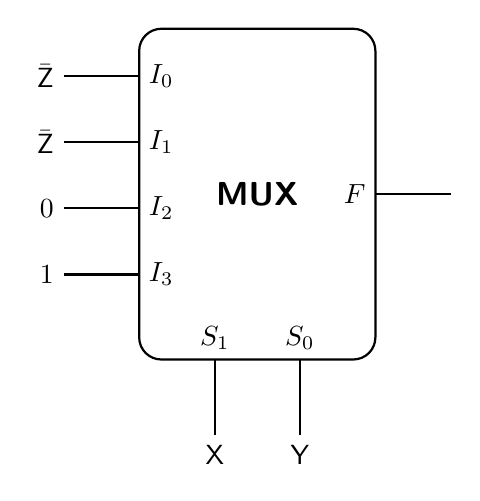
\begin{tikzpicture}[font=\sffamily, scale=1.2]
    % MUX Box
    \draw[thick, rounded corners=8pt] (0,0) rectangle (2.5,3.5);
    \node at (1.25,1.75) {\large \textbf{MUX}};

    % Left Inputs (Lines and Labels)
    % I0
    \draw[thick] (-0.8,3.0) -- (0,3.0);
    \node[left] at (-0.8,3.0) {$\bar{\text{Z}}$};
    \node[right] at (0,3.0) {$I_0$};
    
    % I1
    \draw[thick] (-0.8,2.3) -- (0,2.3);
    \node[left] at (-0.8,2.3) {$\bar{\text{Z}}$};
    \node[right] at (0,2.3) {$I_1$};
    
    % I2
    \draw[thick] (-0.8,1.6) -- (0,1.6);
    \node[left] at (-0.8,1.6) {$0$};
    \node[right] at (0,1.6) {$I_2$};
    
    % I3
    \draw[thick] (-0.8,0.9) -- (0,0.9);
    \node[left] at (-0.8,0.9) {$1$};
    \node[right] at (0,0.9) {$I_3$};

    % Bottom Select Lines
    % S1 / X
    \draw[thick] (0.8,-0.8) -- (0.8,0);
    \node[above] at (0.8,0) {$S_1$};
    \node[below] at (0.8,-0.8) {X};
    
    % S0 / Y
    \draw[thick] (1.7,-0.8) -- (1.7,0);
    \node[above] at (1.7,0) {$S_0$};
    \node[below] at (1.7,-0.8) {Y};

    % Right Output Line
    \draw[thick] (2.5,1.75) -- (3.3,1.75);
    \node[left] at (2.5,1.75) {$F$};

\end{tikzpicture}
\end{center}

\mk{12} \yr{CSE 205 | L-2/T-1 | 2021--22}

\begin{tcolorbox}[enhanced,breakable,ansbox,colback=cD!4,colframe=cD,boxrule=0.8pt,arc=5pt,title={\textbf{Answer}},fonttitle=\bfseries\color{white},colbacktitle=cD]

\subsection*{1. Problem Analysis \& Characteristic Equation}
The logic function implemented by a $4 \times 1$ Multiplexer is defined by its standard characteristic equation:
\begin{align*}
    F(S_1, S_0) &= \overline{S_1}\overline{S_0}I_0 + \overline{S_1}S_0I_1 + S_1\overline{S_0}I_2 + S_1S_0I_3
\end{align*}
Based on the provided problem description, we map the variables to the MUX ports as follows:
\begin{itemize}
    \item \textbf{Selection Lines:} $S_1 = X$ (MSB) and $S_0 = Y$
    \item \textbf{Data Inputs:} $I_0 = \overline{Z}$, $I_1 = Z$, $I_2 = 0$, and $I_3 = 1$
\end{itemize}

Substituting these mappings into the characteristic equation yields the Boolean function in terms of $X, Y,$ and $Z$:
\begin{align*}
    F(X, Y, Z) &= \overline{X}\overline{Y}(\overline{Z}) + \overline{X}Y(Z) + X\overline{Y}(0) + XY(1) \\
    &= \overline{X}\overline{Y}\overline{Z} + \overline{X}YZ + XY \quad \text{(Applying Zero Property and Identity Law)}
\end{align*}

\vspace{0.2cm}
\subsection*{2. Canonical Sum of Products (SOP) Expansion}
To find the maxterms reliably, we first determine the active minterms by expanding the function into its canonical Sum of Products (SOP) form. The term $XY$ is missing the variable $Z$, so we expand it using the Boolean rule $Z + \overline{Z} = 1$:
\begin{align*}
    F(X, Y, Z) &= \overline{X}\overline{Y}\overline{Z} + \overline{X}YZ + XY(Z + \overline{Z}) \\
    &= \overline{X}\overline{Y}\overline{Z} + \overline{X}YZ + XYZ + XY\overline{Z}
\end{align*}
Next, we translate each product term into its corresponding binary combination and minterm notation ($m_i$):
\begin{itemize}
    \item $\overline{X}\overline{Y}\overline{Z} \rightarrow 000_2 \rightarrow m_0$
    \item $\overline{X}YZ \rightarrow 011_2 \rightarrow m_3$
    \item $XY\overline{Z} \rightarrow 110_2 \rightarrow m_6$
    \item $XYZ \rightarrow 111_2 \rightarrow m_7$
\end{itemize}
Thus, the canonical SOP form is:
\[ F(X, Y, Z) = \Sigma\,m(0, 3, 6, 7) \]

\vspace{0.2cm}
\subsection*{3. Conversion to Product of Maxterms (POS)}
For any Boolean function of $n$ variables, the maxterms ($M_j$) represent the input combinations for which the function evaluates to logic $0$. The set of maxterms is the exact complement of the set of minterms with respect to the universal set of indices $0$ to $2^n - 1$.
\\
Since $n = 3$ (for variables $X, Y, Z$), the indices range from $0$ to $7$. Extracting the missing indices from our minterm set gives the maxterm set:
\[ \text{Maxterms} = \{0, 1, 2, 3, 4, 5, 6, 7\} \setminus \{0, 3, 6, 7\} = \{1, 2, 4, 5\} \]

Therefore, the output function in Product of Maxterms (POS) form is:
\begin{align*}
    \mathbf{F(X, Y, Z) = \Pi\,M(1, 2, 4, 5)}
\end{align*}

\vspace{0.2cm}
\subsection*{4. Truth Table Verification}
To guarantee mathematical flawlessness, we verify the output logic across all possible combinations of $X, Y, Z$.

\begin{center}
\renewcommand{\arraystretch}{1.2}
\begin{tabular}{ccc | c | c | l}
\toprule
\textbf{$X \ (S_1)$} & \textbf{$Y \ (S_0)$} & \textbf{$Z$} & \textbf{Active MUX Input} & \textbf{$F$} & \textbf{Classification} \\
\midrule
0 & 0 & 0 & \multirow{2}{*}{$I_0 = \overline{Z}$} & $\mathbf{1}$ & Minterm $m_0$ \\
0 & 0 & 1 & & $\textcolor{cD}{\mathbf{0}}$ & \textcolor{cD}{\textbf{Maxterm $\mathbf{M_1}$}} \\
\midrule
0 & 1 & 0 & \multirow{2}{*}{$I_1 = Z$} & $\textcolor{cD}{\mathbf{0}}$ & \textcolor{cD}{\textbf{Maxterm $\mathbf{M_2}$}} \\
0 & 1 & 1 & & $\mathbf{1}$ & Minterm $m_3$ \\
\midrule
1 & 0 & 0 & \multirow{2}{*}{$I_2 = 0$} & $\textcolor{cD}{\mathbf{0}}$ & \textcolor{cD}{\textbf{Maxterm $\mathbf{M_4}$}} \\
1 & 0 & 1 & & $\textcolor{cD}{\mathbf{0}}$ & \textcolor{cD}{\textbf{Maxterm $\mathbf{M_5}$}} \\
\midrule
1 & 1 & 0 & \multirow{2}{*}{$I_3 = 1$} & $\mathbf{1}$ & Minterm $m_6$ \\
1 & 1 & 1 & & $\mathbf{1}$ & Minterm $m_7$ \\
\bottomrule
\end{tabular}
\end{center}

The truth table visually confirms that the function generates a `0` exclusively at indices $1, 2, 4,$ and $5$, perfectly validating the analytical POS derivation.

\end{tcolorbox}

\item Math teacher Mina Rahman sent sixteen question choices $Q_0,\ldots,Q_{15}$ to her students with a 2-bit binary code $C_1C_0$. If $C_1C_0=11$, $Q_0$ is selected; $C_1C_0=10$, $Q_1$ is selected; \ldots and so on. The code is activated by active-low $\overline{EN_1}$ and active-high $EN_2$. Design the multiplexing circuit.
\mk{15} \yr{CSE 205 | L-2/T-1 | 2020--21}

\begin{tcolorbox}[enhanced,breakable,ansbox,colback=cD!4,colframe=cD,boxrule=0.8pt,arc=5pt,title={\textbf{Answer}},fonttitle=\bfseries\color{white},colbacktitle=cD]

\subsection*{1. Problem Analysis \& Clarification}
The problem states that there are sixteen question choices ($Q_0, \ldots, Q_{15}$) but provides only a 2-bit binary selection code ($C_1C_0$). In digital logic, an $n$-bit selection code can uniquely address exactly $2^n$ inputs. Therefore, a 2-bit code ($C_1C_0$) yields $2^2 = 4$ unique combinations. 

To create a mathematically sound multiplexing circuit based on the specific selection sequence provided in the problem, we will design a \textbf{4-to-1 Multiplexer (MUX)} addressing the four specified choices ($Q_0, Q_1, Q_2, Q_3$). 
\textit{Note: If a 16-to-1 selection was strictly required, the system would necessitate a 4-bit selection code ($C_3C_2C_1C_0$).}

\vspace{0.2cm}
\subsection*{2. Selection Logic \& Variable Mapping}
Based on the defined behavior, the selection sequence is inverted compared to standard binary weighting. We map the variables as follows:
\begin{itemize}
    \item \textbf{Selection Lines:} $S_1 = C_1$ (MSB) and $S_0 = C_0$ (LSB).
    \item \textbf{Enable Logic:} The MUX is active only when $\overline{EN_1} = 0$ (active-low) and $EN_2 = 1$ (active-high). 
    \item \textbf{Data Input Mapping:}
    \begin{itemize}
        \item When $C_1C_0 = 11$ (Decimal 3), $Q_0$ is selected $\implies I_3 = Q_0$
        \item When $C_1C_0 = 10$ (Decimal 2), $Q_1$ is selected $\implies I_2 = Q_1$
        \item When $C_1C_0 = 01$ (Decimal 1), $Q_2$ is selected $\implies I_1 = Q_2$
        \item When $C_1C_0 = 00$ (Decimal 0), $Q_3$ is selected $\implies I_0 = Q_3$
    \end{itemize}
\end{itemize}

\vspace{0.2cm}
\subsection*{3. Truth Table and Boolean Expression}
Let the global Enable signal be $E$. The circuit operates correctly only when $E=1$.
\[ E = (\overline{EN_1})' \cdot EN_2 \]

\begin{center}
\renewcommand{\arraystretch}{1.2}
\begin{tabular}{cc | cc | c | c}
\toprule
\multicolumn{2}{c|}{\textbf{Enable Inputs}} & \multicolumn{2}{c|}{\textbf{Selection Lines}} & \textbf{Internal} & \textbf{Output} \\
$\overline{EN_1}$ & $EN_2$ & $C_1 \ (S_1)$ & $C_0 \ (S_0)$ & \textbf{Enable ($E$)} & \textbf{$Y$} \\
\midrule
1 & X & X & X & 0 & 0 (High-Z/Inactive) \\
X & 0 & X & X & 0 & 0 (High-Z/Inactive) \\
\midrule
0 & 1 & 0 & 0 & 1 & \textcolor{cD}{\textbf{$Q_3$}} \\
0 & 1 & 0 & 1 & 1 & \textcolor{cD}{\textbf{$Q_2$}} \\
0 & 1 & 1 & 0 & 1 & \textcolor{cD}{\textbf{$Q_1$}} \\
0 & 1 & 1 & 1 & 1 & \textcolor{cD}{\textbf{$Q_0$}} \\
\bottomrule
\end{tabular}
\end{center}

The characteristic equation for the active multiplexer is:
\begin{align*}
    Y &= E \cdot \left( \overline{S_1}\overline{S_0}I_0 + \overline{S_1}S_0I_1 + S_1\overline{S_0}I_2 + S_1S_0I_3 \right) \\
    Y &= \left( (\overline{EN_1})' \cdot EN_2 \right) \cdot \left( \overline{C_1}\overline{C_0}Q_3 + \overline{C_1}C_0Q_2 + C_1\overline{C_0}Q_1 + C_1C_0Q_0 \right)
\end{align*}

\vspace{0.4cm}
\subsection*{4. Logic Circuit Implementation}

\begin{center}
\begin{circuitikz}[scale=1.1, transform shape, thick]
    
    % MUX Box
    \draw[fill=white, rounded corners=2pt] (0, 0) rectangle (3, 6);
    \node[align=center, font=\bfseries] at (1.5, 3) {4-to-1 \\ MUX};

    % Select Lines
    \draw[<-] (1, 0) -- (1, -1.5) node[below, font=\bfseries, scale=0.7] {$S_1 \ (C_1)$};
    \draw[<-] (2, 0) -- (2, -1.5) node[below, font=\bfseries, scale=0.7] {$S_0 \ (C_0)$};

    % Enable Logic (AND gate with one inverted input)
    \node[and port, scale=0.75, fill=cD!10, draw=cD] (and1) at (-1.5, 7.5) {};
    \node[not port, scale=0.5, fill=cD!10, draw=cD] (not1) at (-3, 7.7) {};
    
    % Connect Enbale pins
    \draw (-4.5, 7.7) node[left, font=\bfseries] {$\overline{EN_1}$} -- (not1.in);
    \draw (not1.out) -- (and1.in 1);
    \draw (-4.5, 7.28) node[left, font=\bfseries] {$EN_2$} -- (and1.in 2);
    
    % Enable line into MUX
    \draw (and1.out) -| (1.5, 6) node[below=2pt, font=\small\bfseries] {$E$};

    % Input Pins on MUX
    \node[right, font=\small\bfseries] at (0, 5) {$I_3$};
    \node[right, font=\small\bfseries] at (0, 3.5) {$I_2$};
    \node[right, font=\small\bfseries] at (0, 2) {$I_1$};
    \node[right, font=\small\bfseries] at (0, 0.5) {$I_0$};

    % Input Connections mapped backwards per the problem description
    \draw[<-] (0, 5) -- (-2, 5) node[left, font=\bfseries] {$Q_0$};
    \draw[<-] (0, 3.5) -- (-2, 3.5) node[left, font=\bfseries] {$Q_1$};
    \draw[<-] (0, 2) -- (-2, 2) node[left, font=\bfseries] {$Q_2$};
    \draw[<-] (0, 0.5) -- (-2, 0.5) node[left, font=\bfseries] {$Q_3$};

    % Output
    \draw[->, thick, draw=cD] (3, 3) -- (4.5, 3) node[right, font=\bfseries, text=cD] {Output ($Y$)};

\end{circuitikz}
\end{center}

\end{tcolorbox}

\item There are 16 electronic turnstile gates in a cricket stadium. The gates are numbered from 0 to 15 denoted by four bits $T_3T_2T_1T_0$. You have to design a digital ticketing system which uses a switch, and the switch has four input lines $I_0, I_1, I_2, I_3$. These lines can be selected by $S_0, S_1$. The switch is activated by two active low enables $EN_1'$ and $EN_2'$. (The selection policy of the switch is as follows. If $S_1S_0 = 00$, $I_0$ is selected; if $S_1S_0 = 01$, $I_1$ is selected; if $S_1S_0 = 10$, $I_2$ is selected; ... so on.). You can have entry to the stadium if you get the ticket for any of the following gate numbers $(1, 3, 4, 6, 7, 9, 12, 15)$. Design the ticketing circuit using the switch.
\mk{15} \yr{CSE 205 | L-2/T-1 | 2020--21}

\begin{tcolorbox}[enhanced,breakable,ansbox,colback=cD!4,colframe=cD,boxrule=0.8pt,arc=5pt,title={\textbf{Answer}},fonttitle=\bfseries\color{white},colbacktitle=cD]

\subsection*{1. Problem Formalization and Variable Mapping}
The stadium gates are represented by a 4-bit number $T_3T_2T_1T_0$, where $T_3$ is the Most Significant Bit (MSB) and $T_0$ is the Least Significant Bit (LSB). The ticketing system allows entry for a specific set of gate numbers, which can be expressed as a Boolean function in canonical Sum of Products (SOP) form:
\[ F(T_3, T_2, T_1, T_0) = \Sigma\,m(1, 3, 4, 6, 7, 9, 12, 15) \]

We are required to implement this function using a switch that acts as a \textbf{4-to-1 Multiplexer (MUX)}. The MUX has:
\begin{itemize}
    \item \textbf{Selection Lines:} $S_1, S_0$. We map the most significant variables to these lines: $S_1 = T_3$ and $S_0 = T_2$.
    \item \textbf{Data Input Lines:} $I_0, I_1, I_2, I_3$. The logic for these will be derived using the remaining variables $T_1$ and $T_0$.
    \item \textbf{Enable Lines:} Two active-low enables, $\overline{EN_1}$ and $\overline{EN_2}$. The MUX is active only when both are connected to Logic $0$ (Ground).
\end{itemize}

\vspace{0.2cm}
\subsection*{2. Multiplexer Implementation Table}
We distribute the 16 minterms across 4 columns corresponding to the $4$ combinations of the select lines ($T_3, T_2$). We then highlight the minterms present in the entry function to determine the boolean expression for each MUX input based on $T_1$ and $T_0$.

\begin{center}
\renewcommand{\arraystretch}{1.3}
\begin{tabular}{c c | c | c | c | c}
\toprule
\multicolumn{2}{c|}{\textbf{Variables}} & \textbf{$I_0$} & \textbf{$I_1$} & \textbf{$I_2$} & \textbf{$I_3$} \\
$T_1$ & $T_0$ & ($T_3=0, T_2=0$) & ($T_3=0, T_2=1$) & ($T_3=1, T_2=0$) & ($T_3=1, T_2=1$) \\
\midrule
0 & 0 & 0 & \textcolor{cD}{\textbf{4}} & 8 & \textcolor{cD}{\textbf{12}} \\
0 & 1 & \textcolor{cD}{\textbf{1}} & 5 & \textcolor{cD}{\textbf{9}} & 13 \\
1 & 0 & 2 & \textcolor{cD}{\textbf{6}} & 10 & 14 \\
1 & 1 & \textcolor{cD}{\textbf{3}} & \textcolor{cD}{\textbf{7}} & 11 & \textcolor{cD}{\textbf{15}} \\
\bottomrule
\end{tabular}
\end{center}

\vspace{0.2cm}
\subsection*{3. Boolean Derivations for MUX Inputs}
Based on the active minterms in each column, we extract and simplify the Boolean expressions for $I_0, I_1, I_2,$ and $I_3$:

\begin{align*}
    \mathbf{I_0} &= \Sigma(1, 3) = \overline{T_1}T_0 + T_1T_0 \\
                 &= T_0(\overline{T_1} + T_1) \quad &&\text{(Distributive Law)} \\
                 &= T_0(1) = \mathbf{T_0} \quad &&\text{(Complement and Identity Laws)} \\[8pt]
    \mathbf{I_1} &= \Sigma(4, 6, 7) = \overline{T_1}\overline{T_0} + T_1\overline{T_0} + T_1T_0 \\
                 &= \overline{T_0}(\overline{T_1} + T_1) + T_1T_0 \quad &&\text{(Distributive Law)} \\
                 &= \overline{T_0} + T_1T_0 \quad &&\text{(Complement Law)} \\
                 &= (\overline{T_0} + T_1)(\overline{T_0} + T_0) \quad &&\text{(Absorption / Distributive Law: } A + \overline{A}B = A + B \text{)} \\
                 &= \mathbf{T_1 + \overline{T_0}} \quad &&\text{(OR operation)} \\[8pt]
    \mathbf{I_2} &= \Sigma(9) = \mathbf{\overline{T_1}T_0} \quad &&\text{(AND operation, minimal form)} \\[8pt]
    \mathbf{I_3} &= \Sigma(12, 15) = \overline{T_1}\overline{T_0} + T_1T_0 \\
                 &= \mathbf{T_1 \odot T_0} \quad &&\text{(XNOR operation)}
\end{align*}

\vspace{0.2cm}
\subsection*{4. Logic Circuit Implementation}

\begin{center}
\begin{circuitikz}[scale=1.1, transform shape, thick]
    
    % MUX Box
    \draw[fill=white, rounded corners=2pt] (0, 0) rectangle (3, 6);
    \node[align=center, font=\bfseries] at (1.5, 3) {Switch \\ (4-to-1 MUX)};

    % Select Lines
    \draw[<-] (1, 0) -- (1, -1.5) node[below, font=\bfseries, scale=0.7] {$S_1 \ (T_3)$};
    \draw[<-] (2, 0) -- (2, -1.5) node[below, font=\bfseries, scale=0.7] {$S_0 \ (T_2)$};

    % Enable Lines (Active Low)
    \draw[<-] (1, 6) -- (1, 7) node[above, font=\bfseries] {$\overline{EN_1}$};
    \draw[<-] (2, 6) -- (2, 7) node[above, font=\bfseries] {$\overline{EN_2}$};
    \draw[fill=white] (1, 6) circle (3pt); % Active low bubble
    \draw[fill=white] (2, 6) circle (3pt); % Active low bubble

    % Input Pins on MUX
    \node[right, font=\small\bfseries] at (0, 5) {$I_0$};
    \node[right, font=\small\bfseries] at (0, 3.5) {$I_1$};
    \node[right, font=\small\bfseries] at (0, 2) {$I_2$};
    \node[right, font=\small\bfseries] at (0, 0.5) {$I_3$};

    % ----------------------------------------------------
    % FIXED WIRING & GATES SECTION
    % ----------------------------------------------------
    
    % Main Input Lines
    \draw (-6, 5) node[left, font=\bfseries] {$T_0$} -- (0, 5); % T0 directly to I0
    \draw (-6, 4.3) node[left, font=\bfseries] {$T_1$} -- (-5.5, 4.3);
    
    % Vertical bus drops for T1 and T0
    \draw (-5.5, 4.3) -- (-5.5, 0); % T1 bus
    \draw (-4.5, 5) -- (-4.5, 0);   % T0 bus
    
    % Junction dots at the top of buses
    \fill (-5.5, 4.3) circle (2pt);
    \fill (-4.5, 5) circle (2pt);

    % ----------------------------------------------------
    % I1 = T1 + T0' (OR Gate)
    \node[or port, scale=0.8, fill=cD!10, draw=cD] (or1) at (-2, 3.5) {};
    % Align NOT gate perfectly with the second input of OR gate
    \node[not port, scale=0.5] (notT0_1) at (-3.5, 0 |- or1.in 2) {};
    
    % Wire T1 to OR pin 1
    \draw (-5.5, 0 |- or1.in 1) -- (or1.in 1);
    \fill (-5.5, 0 |- or1.in 1) circle (2pt);
    
    % Wire T0 to NOT, then to OR pin 2
    \draw (-4.5, 0 |- notT0_1.in) -- (notT0_1.in);
    \fill (-4.5, 0 |- notT0_1.in) circle (2pt);
    \draw (notT0_1.out) -- (or1.in 2);
    
    % Connect OR output to MUX
    \draw (or1.out) -- (0, 3.5);

    % ----------------------------------------------------
    % I2 = T1' . T0 (AND Gate)
    \node[and port, scale=0.8, fill=cD!10, draw=cD] (and1) at (-2, 2) {};
    % Align NOT gate perfectly with the first input of AND gate
    \node[not port, scale=0.5] (notT1_1) at (-3.5, 0 |- and1.in 1) {};
    
    % Wire T1 to NOT, then to AND pin 1
    \draw (-5.5, 0 |- notT1_1.in) -- (notT1_1.in);
    \fill (-5.5, 0 |- notT1_1.in) circle (2pt);
    \draw (notT1_1.out) -- (and1.in 1);
    
    % Wire T0 to AND pin 2
    \draw (-4.5, 0 |- and1.in 2) -- (and1.in 2);
    \fill (-4.5, 0 |- and1.in 2) circle (2pt);
    
    % Connect AND output to MUX
    \draw (and1.out) -- (0, 2);

    % ----------------------------------------------------
    % I3 = T1 XNOR T0
    \node[xnor port, scale=0.8, fill=cD!10, draw=cD] (xnor1) at (-2, 0.5) {};
    
    % Wire T1 to XNOR pin 1
    \draw (-5.5, 0 |- xnor1.in 1) -- (xnor1.in 1);
    \fill (-5.5, 0 |- xnor1.in 1) circle (2pt);
    
    % Wire T0 to XNOR pin 2
    \draw (-4.5, 0 |- xnor1.in 2) -- (xnor1.in 2);
    \fill (-4.5, 0 |- xnor1.in 2) circle (2pt);
    
    % Connect XNOR output to MUX
    \draw (xnor1.out) -- (0, 0.5);

    % ----------------------------------------------------
    % Output
    \draw[->, draw=cD] (3, 3) -- (5, 3) node[right, font=\bfseries, text=cD, align=left] {Gate \\ Unlock ($F$)};

\end{circuitikz}
\end{center}

\end{tcolorbox}

\item Implement $F(A,B,C,D) = \Sigma\,(1,2,4,10,12,13,14,15)$ with a $4\times1$ multiplexer and external gates. Connect inputs $A$ and $B$ to the selection lines. Express $F$ as a function of $C$ and $D$ for each of the four cases $AB=00,01,10,11$ to obtain the data-line requirements.
\mk{17} \yr{CSE 205 | L-2/T-1 | 2019--20}

\begin{tcolorbox}[enhanced,breakable,ansbox,colback=cD!4,colframe=cD,boxrule=0.8pt,arc=5pt,title={\textbf{Answer}},fonttitle=\bfseries\color{white},colbacktitle=cD]

\subsection*{1. Problem Analysis and Implementation Strategy}
We are tasked with implementing a 4-variable Boolean function $F(A,B,C,D) = \Sigma\,(1,2,4,10,12,13,14,15)$ using a $4 \times 1$ multiplexer. 

A $4 \times 1$ MUX has $2$ select lines and $4$ data inputs. The problem specifies connecting inputs $A$ and $B$ to the select lines:
\begin{itemize}
    \item \textbf{Selection Lines:} $S_1 = A$ (MSB) and $S_0 = B$ (LSB).
    \item \textbf{Data Lines ($I_0, I_1, I_2, I_3$):} The remaining variables, $C$ and $D$, will dictate the logic expressions applied to the input lines for each of the four combinations of $AB$.
\end{itemize}

\vspace{0.2cm}
\subsection*{2. Multiplexer Implementation Table}
We map the 16 minterms of the 4 variables across 4 columns corresponding to the states of $AB$. We highlight the minterms specified in the function to determine the residual logic required from variables $C$ and $D$.

\begin{center}
\renewcommand{\arraystretch}{1.3}
\begin{tabular}{c c | c | c | c | c}
\toprule
\multicolumn{2}{c|}{\textbf{Variables}} & \textbf{$I_0$} & \textbf{$I_1$} & \textbf{$I_2$} & \textbf{$I_3$} \\
$C$ & $D$ & ($A=0, B=0$) & ($A=0, B=1$) & ($A=1, B=0$) & ($A=1, B=1$) \\
\midrule
0 & 0 & 0 & \textcolor{cD}{\textbf{4}} & 8 & \textcolor{cD}{\textbf{12}} \\
0 & 1 & \textcolor{cD}{\textbf{1}} & 5 & 9 & \textcolor{cD}{\textbf{13}} \\
1 & 0 & \textcolor{cD}{\textbf{2}} & 6 & \textcolor{cD}{\textbf{10}} & \textcolor{cD}{\textbf{14}} \\
1 & 1 & 3 & 7 & 11 & \textcolor{cD}{\textbf{15}} \\
\bottomrule
\end{tabular}
\end{center}

\vspace{0.2cm}
\subsection*{3. Boolean Derivations for Data Lines}
By analyzing the active minterms in each column as a function of $C$ and $D$, we systematically derive the minimal Boolean expression for each MUX input:

\begin{align*}
    \mathbf{I_0 \ (AB=00)} &= \Sigma(1, 2) = \overline{C}D + C\overline{D} \\
    &= \mathbf{C \oplus D} \quad &&\text{(Definition of XOR operation)} \\[8pt]
    \mathbf{I_1 \ (AB=01)} &= \Sigma(4) = \overline{C}\overline{D} \\
    &= \mathbf{\overline{C + D}} \quad &&\text{(De Morgan's Law - NOR operation)} \\[8pt]
    \mathbf{I_2 \ (AB=10)} &= \Sigma(10) = \mathbf{C\overline{D}} \quad &&\text{(AND operation with inverted D)} \\[8pt]
    \mathbf{I_3 \ (AB=11)} &= \Sigma(12, 13, 14, 15) = \overline{C}\overline{D} + \overline{C}D + C\overline{D} + CD \\
    &= \overline{C}(\overline{D} + D) + C(\overline{D} + D) \quad &&\text{(Distributive Law)} \\
    &= \overline{C}(1) + C(1) \quad &&\text{(Complement Law: } X + \overline{X} = 1 \text{)} \\
    &= \overline{C} + C = \mathbf{1} \quad &&\text{(Identity and Complement Laws)}
\end{align*}

\vspace{0.2cm}
\subsection*{4. Logic Circuit Implementation}
Using the derived input expressions, we construct the circuit with standard logic gates feeding into the $4 \times 1$ MUX.

\begin{center}
\begin{circuitikz}[scale=1.1, transform shape, thick]
    
    % MUX Box
    \draw[fill=white, rounded corners=2pt] (0, 0) rectangle (3, 6);
    \node[align=center, font=\bfseries] at (1.5, 3) {4-to-1 \\ MUX};

    % Select Lines
    \draw[<-] (1, 0) -- (1, -1.5) node[below, font=\bfseries, scale=0.7] {$S_1 \ (A)$};
    \draw[<-] (2, 0) -- (2, -1.5) node[below, font=\bfseries, scale=0.7] {$S_0 \ (B)$};

    % Input Pins on MUX
    \node[right, font=\small\bfseries] at (0, 5) {$I_0$};
    \node[right, font=\small\bfseries] at (0, 3.5) {$I_1$};
    \node[right, font=\small\bfseries] at (0, 2) {$I_2$};
    \node[right, font=\small\bfseries] at (0, 0.5) {$I_3$};

    % Vertical distribution lines for C and D
    \draw (-6.5, 5.5) node[above, font=\bfseries] {$C$} -- (-6.5, 1.5);
    \draw (-5.5, 5.5) node[above, font=\bfseries] {$D$} -- (-5.5, 1.5);

    % I0 = C XOR D
    \node[xor port, scale=0.8, fill=cD!10, draw=cD] (xor1) at (-2, 5) {};
    \draw (-6.5, 5.2) -- (xor1.in 1);
    \fill (-6.5, 5.2) circle (2pt);
    \draw (-5.5, 4.8) -- (xor1.in 2);
    \fill (-5.5, 4.8) circle (2pt);
    \draw (xor1.out) -- (0, 5);

    % I1 = C NOR D
    \node[nor port, scale=0.8, fill=cD!10, draw=cD] (nor1) at (-2, 3.5) {};
    \draw (-6.5, 3.7) -- (nor1.in 1);
    \fill (-6.5, 3.7) circle (2pt);
    \draw (-5.5, 3.3) -- (nor1.in 2);
    \fill (-5.5, 3.3) circle (2pt);
    \draw (nor1.out) -- (0, 3.5);

    % I2 = C AND D'
    \node[and port, scale=0.8, fill=cD!10, draw=cD] (and1) at (-2, 2) {};
    \node[not port, scale=0.5] (notD) at (-3.5, 1.8) {};
    \draw (-6.5, 2.2) -- (and1.in 1);
    \fill (-6.5, 2.2) circle (2pt);
    \draw (-5.5, 1.8) -- (notD.in);
    \fill (-5.5, 1.8) circle (2pt);
    \draw (notD.out) -- (and1.in 2);
    \draw (and1.out) -- (0, 2);

    % I3 = Logic 1
    \draw[<-] (0, 0.5) -- (-1.5, 0.5) node[left, font=\bfseries] {$1 \ (V_{cc})$};

    % Output
    \draw[->, thick, draw=cD] (3, 3) -- (4.5, 3) node[right, font=\bfseries, text=cD] {$F$};

\end{circuitikz}
\end{center}

\end{tcolorbox}

\item Using a $4\times1$ line MUX, design a logic circuit for $f(w,x,y,z) = \Pi\,(0,2,5,6,7,8,9,10)$, where the MUX has selector bits $S_1S_0$, input lines $I_0\ldots I_3$, active-low enable $\overline{EN_1}$ and active-high enable $EN_2$.
\mk{15} \yr{CSE 205 | L-2/T-1 | 2018--19}

\begin{tcolorbox}[enhanced,breakable,ansbox,colback=cD!4,colframe=cD,boxrule=0.8pt,arc=5pt,title={\textbf{Answer}},fonttitle=\bfseries\color{white},colbacktitle=cD]

\subsection*{1. Problem Analysis and Canonical Conversion}
The given Boolean function is defined in Product of Maxterms (POS) form:
\[ f(w, x, y, z) = \Pi\,(0, 2, 5, 6, 7, 8, 9, 10) \]

To implement this using a Multiplexer (MUX), it is more systematic to express the function in its canonical Sum of Minterms (SOP) form. For a 4-variable function, the universal set of indices is $0$ to $2^4 - 1 = 15$. The minterms are the indices missing from the maxterm list:
\begin{align*}
    \text{Minterms} &= \{0, 1, \dots, 15\} \setminus \{0, 2, 5, 6, 7, 8, 9, 10\} \\
    &= \{1, 3, 4, 11, 12, 13, 14, 15\}
\end{align*}
Thus, the equivalent SOP expression is:
\[ f(w, x, y, z) = \Sigma\,(1, 3, 4, 11, 12, 13, 14, 15) \]

\vspace{0.2cm}
\subsection*{2. Multiplexer Variable Mapping}
A $4 \times 1$ multiplexer requires 2 selection lines ($S_1, S_0$) to address its 4 input lines ($I_0, I_1, I_2, I_3$). We map the most significant variables to the selection lines:
\begin{itemize}
    \item \textbf{Selection Lines:} $S_1 = w$ and $S_0 = x$.
    \item \textbf{Data Lines:} The logic for inputs $I_0, I_1, I_2, I_3$ will be determined as functions of the remaining variables, $y$ and $z$.
\end{itemize}

\vspace{0.2cm}
\subsection*{3. Implementation Table}
We distribute the 16 possible minterms across 4 columns according to the combinations of $w$ and $x$. We then highlight the active minterms belonging to the function to extract the logic expression for each MUX input.

\begin{center}
\renewcommand{\arraystretch}{1.3}
\begin{tabular}{c c | c | c | c | c}
\toprule
\multicolumn{2}{c|}{\textbf{Variables}} & \textbf{$I_0$} & \textbf{$I_1$} & \textbf{$I_2$} & \textbf{$I_3$} \\
$y$ & $z$ & ($w=0, x=0$) & ($w=0, x=1$) & ($w=1, x=0$) & ($w=1, x=1$) \\
\midrule
0 & 0 & 0 & \textcolor{cD}{\textbf{4}} & 8 & \textcolor{cD}{\textbf{12}} \\
0 & 1 & \textcolor{cD}{\textbf{1}} & 5 & 9 & \textcolor{cD}{\textbf{13}} \\
1 & 0 & 2 & 6 & 10 & \textcolor{cD}{\textbf{14}} \\
1 & 1 & \textcolor{cD}{\textbf{3}} & 7 & \textcolor{cD}{\textbf{11}} & \textcolor{cD}{\textbf{15}} \\
\bottomrule
\end{tabular}
\end{center}

\vspace{0.2cm}
\subsection*{4. Boolean Derivations for Input Lines}
We formulate the minimum Boolean expression for each input column based on the active minterms:

\begin{align*}
    \mathbf{I_0 \ (wx=00)} &= \Sigma(1, 3) = \overline{y}z + yz \\
    &= z(\overline{y} + y) \quad &&\text{(Distributive Law)} \\
    &= z(1) = \mathbf{z} \quad &&\text{(Complement and Identity Laws)} \\[8pt]
    \mathbf{I_1 \ (wx=01)} &= \Sigma(4) = \mathbf{\overline{y}\overline{z}} \\
    &= \mathbf{\overline{y + z}} \quad &&\text{(De Morgan's Law - NOR operation)} \\[8pt]
    \mathbf{I_2 \ (wx=10)} &= \Sigma(11) = \mathbf{yz} \quad &&\text{(AND operation)} \\[8pt]
    \mathbf{I_3 \ (wx=11)} &= \Sigma(12, 13, 14, 15) = \overline{y}\overline{z} + \overline{y}z + y\overline{z} + yz \\
    &= \overline{y}(\overline{z} + z) + y(\overline{z} + z) \quad &&\text{(Distributive Law)} \\
    &= \overline{y}(1) + y(1) \quad &&\text{(Complement Law: } A + \overline{A} = 1 \text{)} \\
    &= \overline{y} + y = \mathbf{1} \quad &&\text{(Identity and Complement Laws)}
\end{align*}

\vspace{0.2cm}
\subsection*{5. Logic Circuit Implementation}
The circuit includes the MUX enables: $\overline{EN_1}$ (active-low) must be tied to Ground ($0$), and $EN_2$ (active-high) must be tied to $V_{CC}$ ($1$) for normal operation.

\begin{center}
\begin{circuitikz}[scale=1.1, transform shape, thick]
    
    % MUX Box
    \draw[fill=white, rounded corners=2pt] (0, 0) rectangle (3, 6);
    \node[align=center, font=\bfseries] at (1.5, 3) {4-to-1 \\ MUX};

    % Select Lines
    \draw[<-] (1, 0) -- (1, -1.5) node[below, font=\bfseries, scale=0.7] {$S_1 \ (w)$};
    \draw[<-] (2, 0) -- (2, -1.5) node[below, font=\bfseries, scale=0.7] {$S_0 \ (x)$};

    % Enable Lines
    \draw[<-] (1, 6) -- (1, 7.5) node[above, font=\bfseries,scale=0.5] {Ground (0)};
    \node[right, font=\small\bfseries] at (1.1, 6.5) {$\overline{EN_1}$};
    \draw[fill=white] (1, 6) circle (3pt); % Active low bubble
    
    \draw[<-] (2, 6) -- (2, 7.5) node[above, font=\bfseries, scale=0.5] {$V_{CC}$ (1)};
    \node[right, font=\small\bfseries] at (2.1, 6.5) {$EN_2$};

    % Input Pins on MUX
    \node[right, font=\small\bfseries] at (0, 5) {$I_0$};
    \node[right, font=\small\bfseries] at (0, 3.5) {$I_1$};
    \node[right, font=\small\bfseries] at (0, 2) {$I_2$};
    \node[right, font=\small\bfseries] at (0, 0.5) {$I_3$};

    % Variable Bus for y and z
    \draw (-6.5, 5.5) node[above, font=\bfseries] {$y$} -- (-6.5, 1.5);
    \draw (-5.5, 5.5) node[above, font=\bfseries] {$z$} -- (-5.5, 1.5);

    % I0 = z
    \draw (-5.5, 5) -- (0, 5);
    \fill (-5.5, 5) circle (2pt);

    % I1 = y NOR z
    \node[nor port, scale=0.8, fill=cD!10, draw=cD] (nor1) at (-2, 3.5) {};
    \draw (-6.5, 3.7) -- (nor1.in 1);
    \fill (-6.5, 3.7) circle (2pt);
    \draw (-5.5, 3.3) -- (nor1.in 2);
    \fill (-5.5, 3.3) circle (2pt);
    \draw (nor1.out) -- (0, 3.5);

    % I2 = y AND z
    \node[and port, scale=0.8, fill=cD!10, draw=cD] (and1) at (-2, 2) {};
    \draw (-6.5, 2.2) -- (and1.in 1);
    \fill (-6.5, 2.2) circle (2pt);
    \draw (-5.5, 1.8) -- (and1.in 2);
    \fill (-5.5, 1.8) circle (2pt);
    \draw (and1.out) -- (0, 2);

    % I3 = 1
    \draw[<-] (0, 0.5) -- (-1.5, 0.5) node[left, font=\bfseries] {$1 \ (V_{CC})$};

    % Output F
    \draw[->, thick, draw=cD] (3, 3) -- (4.5, 3) node[right, font=\bfseries, text=cD] {$f(w,x,y,z)$};

\end{circuitikz}
\end{center}

\end{tcolorbox}

\item Design a 1-bit Full Subtractor using a $4\times1$ multiplexer. The MUX has selector bits $S_1S_0$, input lines $I_0, I_1, I_2, I_3$, and active-low enable $\overline{EN}$.
\mk{12} \yr{CSE 205 | L-2/T-1 | 2018--19}

\begin{tcolorbox}[enhanced,breakable,ansbox,colback=cD!4,colframe=cD,boxrule=0.8pt,arc=5pt,title={\textbf{Answer}},fonttitle=\bfseries\color{white},colbacktitle=cD]

\subsection*{1. Truth Table of a 1-Bit Full Subtractor}
A 1-bit Full Subtractor subtracts a subtrahend ($Y$) and a borrow-in ($B_{in}$) from a minuend ($X$). It produces two outputs: Difference ($D$) and Borrow-out ($B_{out}$). The truth table defining this behavior is:

\begin{center}
\renewcommand{\arraystretch}{1.2}
\begin{tabular}{ccc | cc}
\toprule
\multicolumn{3}{c|}{\textbf{Inputs}} & \multicolumn{2}{c}{\textbf{Outputs}} \\
$X$ (Minuend) & $Y$ (Subtrahend) & $B_{in}$ (Borrow In) & \textbf{$D$ (Difference)} & \textbf{$B_{out}$ (Borrow Out)} \\
\midrule
0 & 0 & 0 & 0 & 0 \\
0 & 0 & 1 & 1 & 1 \\
\midrule
0 & 1 & 0 & 1 & 1 \\
0 & 1 & 1 & 0 & 1 \\
\midrule
1 & 0 & 0 & 1 & 0 \\
1 & 0 & 1 & 0 & 0 \\
\midrule
1 & 1 & 0 & 0 & 0 \\
1 & 1 & 1 & 1 & 1 \\
\bottomrule
\end{tabular}
\end{center}

\vspace{0.2cm}
\subsection*{2. Multiplexer Configuration Strategy}
Since a Full Subtractor has two independent output functions ($D$ and $B_{out}$), we require \textbf{two} $4 \times 1$ multiplexers. 
\begin{itemize}
    \item \textbf{Selection Lines:} We assign the variables $X$ and $Y$ to the MUX selector bits: $S_1 = X$ and $S_0 = Y$.
    \item \textbf{Data Lines ($I_0, I_1, I_2, I_3$):} The inputs for each MUX will be evaluated as a function of the remaining variable, $B_{in}$.
    \item \textbf{Enable Line:} The problem specifies an active-low enable ($\overline{EN}$). For the MUX to function, this line must be tied to Logic $0$ (Ground).
\end{itemize}

\vspace{0.2cm}
\subsection*{3. Boolean Derivation for Data Lines}
We determine the input data lines algebraically by fixing the selection lines $X$ and $Y$, and expressing the output solely in terms of $B_{in}$.

\subsubsection*{A. Difference Output ($D$)}
The standard Boolean expression for the Difference is $D = X \oplus Y \oplus B_{in}$. Let's evaluate this for all four selector combinations:
\begin{align*}
    \mathbf{I_0 \ (XY=00):} \quad D &= 0 \oplus 0 \oplus B_{in} \\
    &= 0 \oplus B_{in} = \textcolor{cD}{\mathbf{B_{in}}} \quad &&\text{(Identity Law of XOR)} \\[6pt]
    \mathbf{I_1 \ (XY=01):} \quad D &= 0 \oplus 1 \oplus B_{in} \\
    &= 1 \oplus B_{in} = \textcolor{cD}{\mathbf{\overline{B_{in}}}} \quad &&\text{(Inversion Law of XOR)} \\[6pt]
    \mathbf{I_2 \ (XY=10):} \quad D &= 1 \oplus 0 \oplus B_{in} \\
    &= 1 \oplus B_{in} = \textcolor{cD}{\mathbf{\overline{B_{in}}}} \quad &&\text{(Inversion Law of XOR)} \\[6pt]
    \mathbf{I_3 \ (XY=11):} \quad D &= 1 \oplus 1 \oplus B_{in} \\
    &= 0 \oplus B_{in} = \textcolor{cD}{\mathbf{B_{in}}} \quad &&\text{(Identity Law of XOR)}
\end{align*}

\subsubsection*{B. Borrow-Out Output ($B_{out}$)}
The standard minimized Boolean expression for Borrow-out is $B_{out} = \overline{X}Y + \overline{X}B_{in} + YB_{in}$.
\begin{align*}
    \mathbf{I_0 \ (XY=00):} \quad B_{out} &= \overline{0}(0) + \overline{0}B_{in} + 0(B_{in}) \\
    &= 0 + 1 \cdot B_{in} + 0 = \textcolor{cD}{\mathbf{B_{in}}} \quad &&\text{(Identity and Annulment Laws)} \\[6pt]
    \mathbf{I_1 \ (XY=01):} \quad B_{out} &= \overline{0}(1) + \overline{0}B_{in} + 1(B_{in}) \\
    &= 1 + B_{in} + B_{in} = \textcolor{cD}{\mathbf{1}} \quad &&\text{(Annulment Law: } 1 + A = 1 \text{)} \\[6pt]
    \mathbf{I_2 \ (XY=10):} \quad B_{out} &= \overline{1}(0) + \overline{1}B_{in} + 0(B_{in}) \\
    &= 0 + 0 \cdot B_{in} + 0 = \textcolor{cD}{\mathbf{0}} \quad &&\text{(Annulment Law: } 0 \cdot A = 0 \text{)} \\[6pt]
    \mathbf{I_3 \ (XY=11):} \quad B_{out} &= \overline{1}(1) + \overline{1}B_{in} + 1(B_{in}) \\
    &= 0 \cdot 1 + 0 \cdot B_{in} + B_{in} = \textcolor{cD}{\mathbf{B_{in}}} \quad &&\text{(Identity and Annulment Laws)}
\end{align*}

\vspace{0.4cm}
\subsection*{4. Logic Circuit Implementation}
Using the derived data lines, we construct the twin $4 \times 1$ MUX circuit for the Full Subtractor.

\begin{center}
\begin{circuitikz}[scale=1.1, transform shape, thick]
    
    % ================= MUX 1: DIFFERENCE =================
    \draw[fill=white, rounded corners=2pt] (0, 0) rectangle (3, 5);
    \node[align=center, scale=0.8, font=\bfseries] at (1.5, 2.5) {4-to-1 MUX \\ (Difference)};

    % Select Lines
    \draw[<-] (1, 0) -- (1, -1) node[below, font=\bfseries, scale=0.8] {$S_1 \ (X)$};
    \draw[<-] (2, 0) -- (2, -1) node[below, font=\bfseries, scale=0.8] {$S_0 \ (Y)$};

    % Enable Line
    \draw[<-] (1.5, 5) -- (1.5, 6) node[above, font=\bfseries] {GND (0)};
    \draw[fill=white] (1.5, 5) circle (3pt); % Active low bubble
    \node[right, font=\small\bfseries] at (1.6, 5.5) {$\overline{EN}$};

    % Input Pins
    \node[right, font=\small\bfseries] at (0, 4) {$I_0$};
    \node[right, font=\small\bfseries] at (0, 3) {$I_1$};
    \node[right, font=\small\bfseries] at (0, 2) {$I_2$};
    \node[right, font=\small\bfseries] at (0, 1) {$I_3$};

    % Data Line Connections
    \draw (-1.5, 4) node[left, font=\bfseries] {$B_{in}$} -- (0, 4);
    \draw (-1.5, 3) node[left, font=\bfseries] {$\overline{B_{in}}$} -- (0, 3);
    \draw (-1.5, 2) node[left, font=\bfseries] {$\overline{B_{in}}$} -- (0, 2);
    \draw (-1.5, 1) node[left, font=\bfseries] {$B_{in}$} -- (0, 1);

    % Output
    \draw[->, draw=cD] (3, 2.5) -- (4.5, 2.5) node[right, font=\bfseries, text=cD] {Difference ($D$)};

\end{circuitikz}

\begin{circuitikz}[scale=1.1, transform shape, thick]

 
        \draw[fill=white, rounded corners=2pt] (0, 0) rectangle (3, 5);
        \node[align=center, scale=0.8, font=\bfseries] at (1.5, 2.5) {4-to-1 MUX \\ (Borrow-Out)};

        % Select Lines
        \draw[<-] (1, 0) -- (1, -1) node[below, font=\bfseries, scale=0.8] {$S_1 \ (X)$};
        \draw[<-] (2, 0) -- (2, -1) node[below, font=\bfseries, scale=0.8] {$S_0 \ (Y)$};

        % Enable Line
        \draw[<-] (1.5, 5) -- (1.5, 6) node[above, font=\bfseries] {GND (0)};
        \draw[fill=white] (1.5, 5) circle (3pt); % Active low bubble
        \node[right, font=\small\bfseries] at (1.6, 5.5) {$\overline{EN}$};

        % Input Pins
        \node[right, font=\small\bfseries] at (0, 4) {$I_0$};
        \node[right, font=\small\bfseries] at (0, 3) {$I_1$};
        \node[right, font=\small\bfseries] at (0, 2) {$I_2$};
        \node[right, font=\small\bfseries] at (0, 1) {$I_3$};

        % Data Line Connections
        \draw (-1.5, 4) node[left, font=\bfseries] {$B_{in}$} -- (0, 4);
        \draw (-1.5, 3) node[left, font=\bfseries] {$1 \ (V_{cc})$} -- (0, 3);
        \draw (-1.5, 2) node[left, font=\bfseries] {$0 \ (GND)$} -- (0, 2);
        \draw (-1.5, 1) node[left, font=\bfseries] {$B_{in}$} -- (0, 1);

        % Output
        \draw[->, draw=cD] (3, 2.5) -- (4.5, 2.5) node[right, font=\bfseries, text=cD] {Borrow-Out ($B_{out}$)};


\end{circuitikz}
\end{center}

\end{tcolorbox}

\item Using an $8\times1$ line MUX, design a logic circuit for $f(w,x,y,z) = \mathrm{POS}(0,2,5,6,7,8,9,10)$, where the MUX has selector bits $S_2S_1S_0$, input lines $I_0\ldots I_7$, and active-low enable $\overline{EN}$. (If $S_2S_1S_0 = 000$, $I_0$ is selected; \ldots and so on.)
\mk{15} \yr{CSE 205 | L-2/T-1 | 2017--18}

\begin{tcolorbox}[enhanced,breakable,ansbox,colback=cD!4,colframe=cD,boxrule=0.8pt,arc=5pt,title={\textbf{Answer}},fonttitle=\bfseries\color{white},colbacktitle=cD]

\textbf{Step 1: Convert the Function to Sum of Products (SOP) Form}

The given boolean function is expressed as a Product of Sums (POS), characterized by its maxterms. Since there are 4 variables ($w, x, y, z$), the total number of fundamental combinations is $2^4 = 16$, corresponding to indices $0$ to $15$. 

We can easily switch from POS to SOP (Sum of Products) by finding the complementary indices, as a function contains either the minterm or the maxterm for every possible input combination:
\begin{align*}
f(w,x,y,z) &= \prod M(0,2,5,6,7,8,9,10) \\
           &= \sum m(1,3,4,11,12,13,14,15)
\end{align*}

\textbf{Step 2: Assign Variables to Multiplexer Control Lines}

We must implement this 4-variable function using an $8\times1$ Multiplexer. An $8\times1$ MUX has $3$ selector lines ($S_2, S_1, S_0$). 
We partition our 4 variables such that the most significant variables are tied to the selectors, and the least significant variable acts as the data input to the MUX.
\begin{itemize}
    \item \textbf{Selector Lines:} Connect $w \rightarrow S_2$, $x \rightarrow S_1$, and $y \rightarrow S_0$.
    \item \textbf{Data Input Variable:} The remaining variable is $z$. Thus, the data inputs $I_0, I_1, \ldots, I_7$ will be derived as functions of $z$ (i.e., $0, 1, z, \text{ or } \overline{z}$).
\end{itemize}

\textbf{Step 3: Construct the Multiplexer Implementation Table}

We create an implementation table mapping the $16$ possible minterms into the $8$ data inputs based on the state of $z$. Each data line $I_k$ controls a pair of minterms: one where $z=0$ (even index) and one where $z=1$ (odd index). We circle or bold the minterms present in our SOP expression to determine the logical expression for each $I_k$.

\begin{center}
\renewcommand{\arraystretch}{1.2}
\begin{tabular}{ccc|c|cc|c}
\toprule
$S_2 (w)$ & $S_1 (x)$ & $S_0 (y)$ & MUX Input & $z = 0$ & $z = 1$ & Logic Function \\
\midrule
$0$ & $0$ & $0$ & $I_0$ & $0$ & $\textcolor{cD}{\mathbf{1}}$ & $I_0 = z$ \\
$0$ & $0$ & $1$ & $I_1$ & $2$ & $\textcolor{cD}{\mathbf{3}}$ & $I_1 = z$ \\
$0$ & $1$ & $0$ & $I_2$ & $\textcolor{cD}{\mathbf{4}}$ & $5$ & $I_2 = \overline{z}$ \\
$0$ & $1$ & $1$ & $I_3$ & $6$ & $7$ & $I_3 = 0$ \\
$1$ & $0$ & $0$ & $I_4$ & $8$ & $9$ & $I_4 = 0$ \\
$1$ & $0$ & $1$ & $I_5$ & $10$ & $\textcolor{cD}{\mathbf{11}}$ & $I_5 = z$ \\
$1$ & $1$ & $0$ & $I_6$ & $\textcolor{cD}{\mathbf{12}}$ & $\textcolor{cD}{\mathbf{13}}$ & $I_6 = 1$ \\
$1$ & $1$ & $1$ & $I_7$ & $\textcolor{cD}{\mathbf{14}}$ & $\textcolor{cD}{\mathbf{15}}$ & $I_7 = 1$ \\
\bottomrule
\end{tabular}
\end{center}

\textbf{Step 4: Circuit Diagram}

The MUX has an active-low enable $\overline{EN}$. For the multiplexer to function normally, this pin must be tied to a logic low state ($0$ or GND). 

\vspace{0.5cm}
\begin{center}
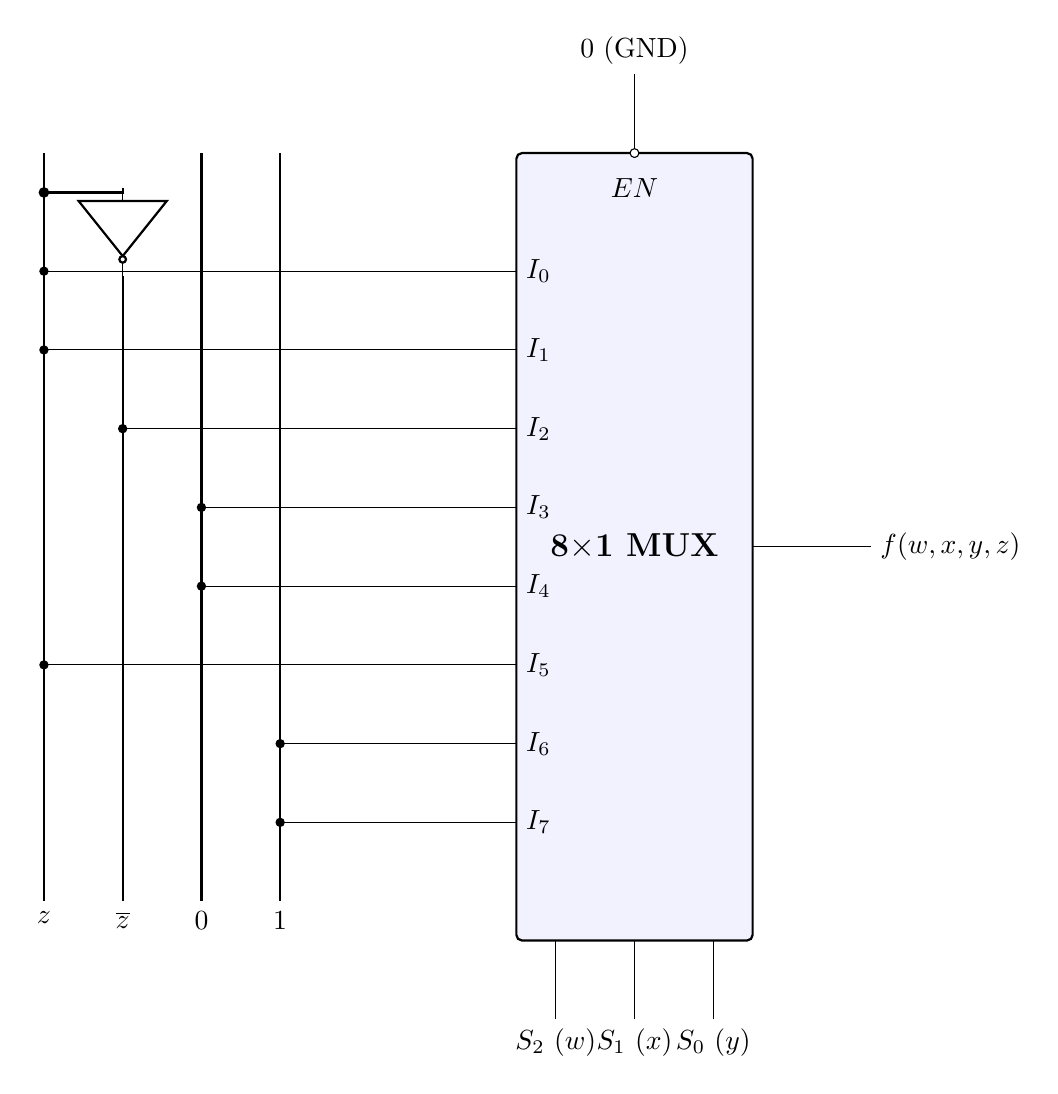
\begin{tikzpicture}

    % Common Data Rails
    \draw[thick] (-4, 9.5) -- (-4, 0) node[below] {$z$};
    
    % Inverter for z_bar
    \node[not port, rotate=-90, scale=0.8] (notz) at (-3, 8.5) {};
    \draw[thick, fill=black] (-4, 9) circle (1.5pt);
    \draw[thick] (-4, 9) -- (-3, 9) -- (notz.in);
    \draw[thick] (notz.out) -- (-3, 0) node[below] {$\overline{z}$};
    
    % Logic 0 and 1 Rails
    \draw[thick] (-2, 9.5) -- (-2, 0) node[below] {$0$};
    \draw[thick] (-1, 9.5) -- (-1, 0) node[below] {$1$};

    % MUX Box
    \draw[thick, fill=blue!5, rounded corners=2pt] (2, -0.5) rectangle (5, 9.5);
    \node at (3.5, 4.5) {\large \textbf{8$\times$1 MUX}};

    % Inputs I0 to I7 Labeling and Connection
    \foreach \i/\y in {0/8, 1/7, 2/6, 3/5, 4/4, 5/3, 6/2, 7/1} {
        \node[right] at (2, \y) {$I_{\i}$};
    }

    % Wiring the Data Rails to MUX Inputs
    % I0 = z
    \draw (-4, 8) node[circle,fill,inner sep=1.2pt]{} -- (2, 8);
    % I1 = z
    \draw (-4, 7) node[circle,fill,inner sep=1.2pt]{} -- (2, 7);
    % I2 = z'
    \draw (-3, 6) node[circle,fill,inner sep=1.2pt]{} -- (2, 6);
    % I3 = 0
    \draw (-2, 5) node[circle,fill,inner sep=1.2pt]{} -- (2, 5);
    % I4 = 0
    \draw (-2, 4) node[circle,fill,inner sep=1.2pt]{} -- (2, 4);
    % I5 = z
    \draw (-4, 3) node[circle,fill,inner sep=1.2pt]{} -- (2, 3);
    % I6 = 1
    \draw (-1, 2) node[circle,fill,inner sep=1.2pt]{} -- (2, 2);
    % I7 = 1
    \draw (-1, 1) node[circle,fill,inner sep=1.2pt]{} -- (2, 1);

    % Selectors
    \draw (2.5, -0.5) -- (2.5, -1.5) node[below] {$S_2 \ (w)$};
    \draw (3.5, -0.5) -- (3.5, -1.5) node[below] {$S_1 \ (x)$};
    \draw (4.5, -0.5) -- (4.5, -1.5) node[below] {$S_0 \ (y)$};

    % Active-Low Enable Pin
    \node[ocirc] (en_node) at (3.5, 9.5) {};
    \node[below] at (3.5, 9.3) {$EN$};
    \draw (en_node.north) -- (3.5, 10.5) node[above] {$0 \ \text{(GND)}$};

    % Output
    \draw (5, 4.5) -- (6.5, 4.5) node[right] {$f(w,x,y,z)$};

\end{tikzpicture}
\end{center}

\end{tcolorbox}

\item Design a 1-bit Full Adder using two $4\times1$ multiplexers. The MUX has selector bits $S_1S_0$, input lines $I_0, I_1, I_2, I_3$, and active-low enable $\overline{EN}$. (If $S_1S_0 = 00$, $I_0$ is selected; $01 \to I_1$; $10 \to I_2$; $11 \to I_3$.)
\mk{12} \yr{CSE 205 | L-2/T-1 | 2017--18}

\begin{tcolorbox}[enhanced,breakable,ansbox,colback=cD!4,colframe=cD,boxrule=0.8pt,arc=5pt,title={\textbf{Answer}},fonttitle=\bfseries\color{white},colbacktitle=cD]

\textbf{Step 1: Truth Table of a 1-bit Full Adder}

A 1-bit full adder computes the sum of three bits: $A, B,$ and $C_{in}$. It produces two outputs: $Sum$ and $C_{out}$ (Carry-out). The truth table for these operations is defined as follows:

\begin{center}
\renewcommand{\arraystretch}{1.2}
\begin{tabular}{ccc|cc}
\toprule
\multicolumn{3}{c|}{\textbf{Inputs}} & \multicolumn{2}{c}{\textbf{Outputs}} \\
$A$ & $B$ & $C_{in}$ & $Sum$ & $C_{out}$ \\
\midrule
$0$ & $0$ & $0$ & $0$ & $0$ \\
$0$ & $0$ & $1$ & $1$ & $0$ \\
\midrule
$0$ & $1$ & $0$ & $1$ & $0$ \\
$0$ & $1$ & $1$ & $0$ & $1$ \\
\midrule
$1$ & $0$ & $0$ & $1$ & $0$ \\
$1$ & $0$ & $1$ & $0$ & $1$ \\
\midrule
$1$ & $1$ & $0$ & $0$ & $1$ \\
$1$ & $1$ & $1$ & $1$ & $1$ \\
\bottomrule
\end{tabular}
\end{center}

\textbf{Step 2: Assign Variables to Multiplexer Selectors}

We are tasked with implementing the two output functions ($Sum$ and $C_{out}$) using two $4\times1$ multiplexers. 
A $4\times1$ MUX requires $2$ selector lines ($S_1, S_0$). We will map the inputs $A$ and $B$ to the selector lines of both multiplexers:
\begin{itemize}
    \item $S_1 = A$
    \item $S_0 = B$
\end{itemize}
The remaining input, $C_{in}$, will be used to derive the data inputs $I_0, I_1, I_2, I_3$ for each MUX.

\vspace{0.5cm}
\textbf{Step 3: Deriving MUX Inputs}

We evaluate the relationship between the outputs and $C_{in}$ for every combination of $A$ and $B$.

\textbf{For the Sum Multiplexer (MUX 1):}
\begin{align*}
    A=0, B=0 \ (S_1 S_0 = 00) &\implies Sum = C_{in} \quad &&\therefore I_0 = C_{in} \\
    A=0, B=1 \ (S_1 S_0 = 01) &\implies Sum = \overline{C_{in}} \quad &&\therefore I_1 = \overline{C_{in}} \\
    A=1, B=0 \ (S_1 S_0 = 10) &\implies Sum = \overline{C_{in}} \quad &&\therefore I_2 = \overline{C_{in}} \\
    A=1, B=1 \ (S_1 S_0 = 11) &\implies Sum = C_{in} \quad &&\therefore I_3 = C_{in}
\end{align*}

\textbf{For the Carry-out Multiplexer (MUX 2):}
\begin{align*}
    A=0, B=0 \ (S_1 S_0 = 00) &\implies C_{out} = 0 \quad &&\therefore I_0 = 0 \\
    A=0, B=1 \ (S_1 S_0 = 01) &\implies C_{out} = C_{in} \quad &&\therefore I_1 = C_{in} \\
    A=1, B=0 \ (S_1 S_0 = 10) &\implies C_{out} = C_{in} \quad &&\therefore I_2 = C_{in} \\
    A=1, B=1 \ (S_1 S_0 = 11) &\implies C_{out} = 1 \quad &&\therefore I_3 = 1
\end{align*}

\vspace{0.2cm}
\textbf{Step 4: Circuit Diagram}

Both multiplexers have an active-low enable $\overline{EN}$. This pin must be tied to a logic low state ($0$ or GND) for normal operation. The data rails provide $0, 1, C_{in},$ and $\overline{C_{in}}$.

\vspace{0.5cm}
\begin{center}
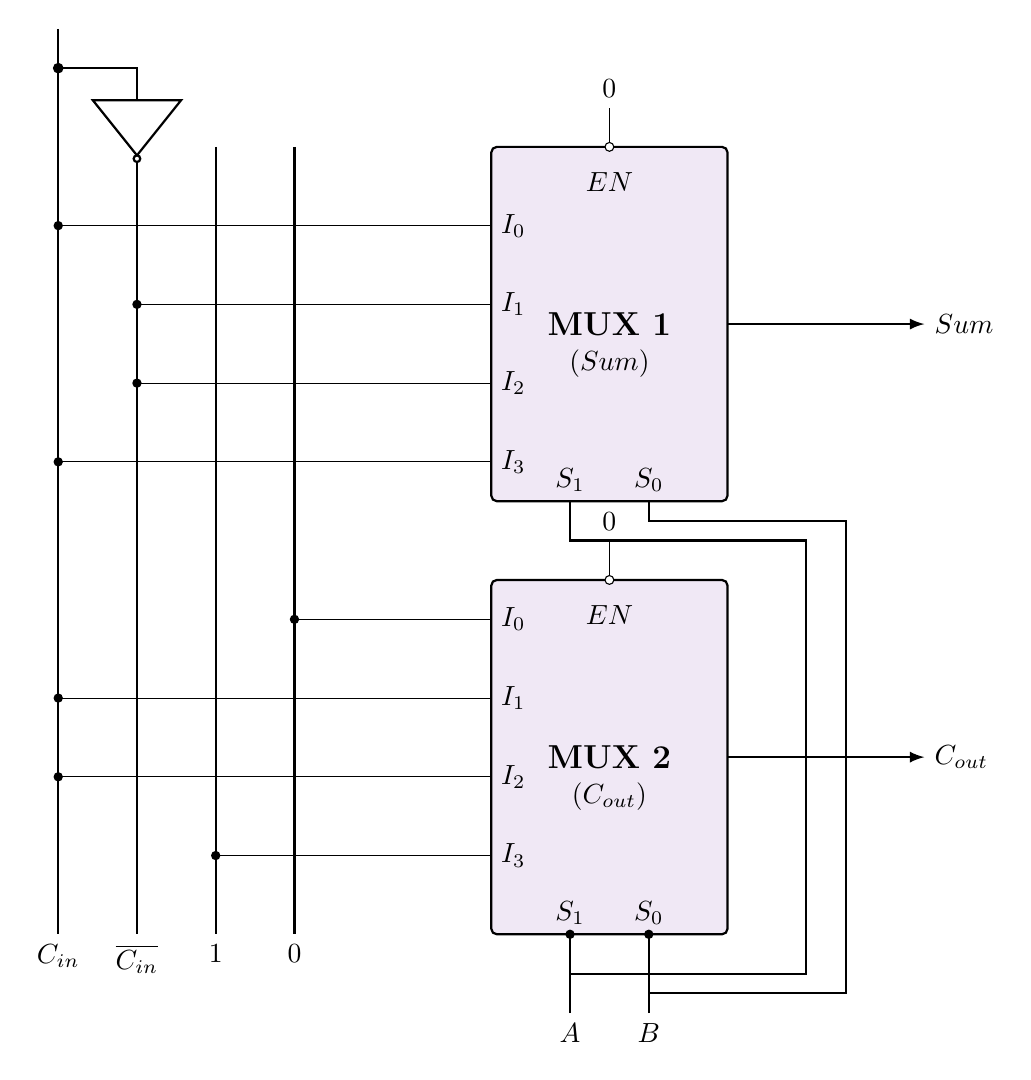
\begin{tikzpicture}[>=latex]

    % Common Data Rails
    \draw[thick] (-4.5, 11.5) -- (-4.5, 0) node[below] {$C_{in}$};
    
    % Inverter for C_in bar
    \node[not port, rotate=-90, scale=0.8] (notc) at (-3.5, 10.2) {};
    \draw[thick, fill=black] (-4.5, 11) circle (1.5pt);
    \draw[thick] (-4.5, 11) -- (-3.5, 11) -- (notc.in);
    \draw[thick] (notc.out) -- (-3.5, 0) node[below] {$\overline{C_{in}}$};
    
    % Logic 0 and 1 Rails
    \draw[thick] (-2.5, 10) -- (-2.5, 0) node[below] {$1$};
    \draw[thick] (-1.5, 10) -- (-1.5, 0) node[below] {$0$};

    % --- MUX 1: SUM ---
    \draw[thick, fill=cD!10, rounded corners=2pt] (1, 5.5) rectangle (4, 10);
    \node at (2.5, 7.75) {\large \textbf{MUX 1}};
    \node at (2.5, 7.25) {($Sum$)};

    % Inputs I0 to I3 Labeling and Connection for MUX 1
    \foreach \i/\y in {0/9, 1/8, 2/7, 3/6} {
        \node[right] at (1, \y) {$I_{\i}$};
    }
    
    % Wiring data to MUX 1
    % I0 = C_in
    \draw (-4.5, 9) node[circle,fill,inner sep=1.2pt]{} -- (1, 9);
    % I1 = C_in_bar
    \draw (-3.5, 8) node[circle,fill,inner sep=1.2pt]{} -- (1, 8);
    % I2 = C_in_bar
    \draw (-3.5, 7) node[circle,fill,inner sep=1.2pt]{} -- (1, 7);
    % I3 = C_in
    \draw (-4.5, 6) node[circle,fill,inner sep=1.2pt]{} -- (1, 6);

    % --- MUX 2: C_OUT ---
    \draw[thick, fill=cD!10, rounded corners=2pt] (1, 0) rectangle (4, 4.5);
    \node at (2.5, 2.25) {\large \textbf{MUX 2}};
    \node at (2.5, 1.75) {($C_{out}$)};

    % Inputs I0 to I3 Labeling and Connection for MUX 2
    \foreach \i/\y in {0/4, 1/3, 2/2, 3/1} {
        \node[right] at (1, \y) {$I_{\i}$};
    }

    % Wiring data to MUX 2
    % I0 = 0
    \draw (-1.5, 4) node[circle,fill,inner sep=1.2pt]{} -- (1, 4);
    % I1 = C_in
    \draw (-4.5, 3) node[circle,fill,inner sep=1.2pt]{} -- (1, 3);
    % I2 = C_in
    \draw (-4.5, 2) node[circle,fill,inner sep=1.2pt]{} -- (1, 2);
    % I3 = 1
    \draw (-2.5, 1) node[circle,fill,inner sep=1.2pt]{} -- (1, 1);

    % --- Selector Pins & Common Bus ---
    % S1, S0 labels inside MUX 1
    \node[above] at (2, 5.5) {$S_1$};
    \node[above] at (3, 5.5) {$S_0$};
    % S1, S0 labels inside MUX 2
    \node[above] at (2, 0) {$S_1$};
    \node[above] at (3, 0) {$S_0$};
    
    % Selector Wires
    \draw[thick] (2, -1) node[below] {$A$} -- (2, 0);
    \draw[thick] (3, -1) node[below] {$B$} -- (3, 0);
    
    % Route selectors from MUX 2 to MUX 1 avoiding inputs
    \draw[thick] (2, 0) node[circle,fill,inner sep=1.2pt]{} -- (2, -0.5) -- (5, -0.5) -- (5, 5) -- (2, 5) -- (2, 5.5);
    \draw[thick] (3, 0) node[circle,fill,inner sep=1.2pt]{} -- (3, -0.75) -- (5.5, -0.75) -- (5.5, 5.25) -- (3, 5.25) -- (3, 5.5);

    % --- Active-Low Enable Pins ---
    % MUX 1 Enable
    \node[ocirc] (en1) at (2.5, 10) {};
    \node[below] at (2.5, 9.8) {$EN$};
    \draw (en1.north) -- (2.5, 10.5) node[above] {$0$};
    
    % MUX 2 Enable
    \node[ocirc] (en2) at (2.5, 4.5) {};
    \node[below] at (2.5, 4.3) {$EN$};
    \draw (en2.north) -- (2.5, 5) node[above] {$0$};

    % --- Output Signals ---
    \draw[thick, ->] (4, 7.75) -- (6.5, 7.75) node[right] {\textbf{$Sum$}};
    \draw[thick, ->] (4, 2.25) -- (6.5, 2.25) node[right] {\textbf{$C_{out}$}};

\end{tikzpicture}
\end{center}

\end{tcolorbox}

\item Using only $4\times1$ line, 2-bit multiplexers, design $f(w,x,y,z) = \pi\,(2,4,5,7,11,12,13)$. (Use minimum gates if required.)
\mk{12} \yr{CSE 205 | L-2/T-1 | 2016--17}

\begin{tcolorbox}[enhanced,breakable,ansbox,colback=cD!4,colframe=cD,boxrule=0.8pt,arc=5pt,title={\textbf{Answer}},fonttitle=\bfseries\color{white},colbacktitle=cD]

\textbf{Step 1: Convert the Function to Sum of Products (SOP) Form}

The given boolean function is provided in Product of Sums (POS) form, specifying the maxterms. For a 4-variable function ($w, x, y, z$), the domain ranges from $0$ to $15$. We convert this to Sum of Products (SOP) by identifying the missing indices, which correspond to the minterms:
\begin{align*}
f(w,x,y,z) &= \prod M(2,4,5,7,11,12,13) \\
           &= \sum m(0,1,3,6,8,9,10,14,15)
\end{align*}

\textbf{Step 2: Multiplexer Tree Design Strategy (Shannon's Expansion)}

The prompt restricts us to using \textbf{only} $4\times1$ line multiplexers. A single $4\times1$ MUX has $2$ selector lines and $4$ data inputs, which inherently evaluates any 2-variable logic function by tying its inputs directly to $0$ or $1$. 

Because we have a 4-variable function and cannot use external logic gates (AND, OR, NOT), we must construct a \textbf{Multiplexer Tree} to form an equivalent $16\times1$ multiplexer. 
\begin{itemize}
    \item \textbf{Level 2 (Output Stage):} A single $4\times1$ MUX controlled by the two Most Significant Bits (MSBs), $w$ and $x$.
    \item \textbf{Level 1 (Input Stage):} Four $4\times1$ MUXes controlled by the two Least Significant Bits (LSBs), $y$ and $z$. The outputs of these four MUXes feed directly into the Output Stage MUX.
\end{itemize}

\textbf{Step 3: Deriving the MUX Data Inputs}

We evaluate the function for all 16 combinations. The bits $w$ and $x$ select which Level 1 MUX is active, while $y$ and $z$ select the specific input ($0, 1, 2,$ or $3$) inside that Level 1 MUX.

\begin{center}
\renewcommand{\arraystretch}{1.3}
\begin{tabular}{cc|cccc|c}
\toprule
\multicolumn{2}{c|}{\textbf{Level 2 Selectors}} & \multicolumn{4}{c|}{\textbf{Minterm Values for $y,z$ ($S_1, S_0$)}} & \textbf{Level 1 MUX} \\
$w \,(S_1)$ & $x \,(S_0)$ & $00 \,(I_0)$ & $01 \,(I_1)$ & $10 \,(I_2)$ & $11 \,(I_3)$ & \textbf{Assignment} \\
\midrule
$0$ & $0$ & $m_0 = \textcolor{cD}{\mathbf{1}}$ & $m_1 = \textcolor{cD}{\mathbf{1}}$ & $m_2 = 0$ & $m_3 = \textcolor{cD}{\mathbf{1}}$ & \textbf{MUX 0} inputs: $1, 1, 0, 1$ \\
$0$ & $1$ & $m_4 = 0$ & $m_5 = 0$ & $m_6 = \textcolor{cD}{\mathbf{1}}$ & $m_7 = 0$ & \textbf{MUX 1} inputs: $0, 0, 1, 0$ \\
$1$ & $0$ & $m_8 = \textcolor{cD}{\mathbf{1}}$ & $m_9 = \textcolor{cD}{\mathbf{1}}$ & $m_{10} = \textcolor{cD}{\mathbf{1}}$ & $m_{11} = 0$ & \textbf{MUX 2} inputs: $1, 1, 1, 0$ \\
$1$ & $1$ & $m_{12} = 0$ & $m_{13} = 0$ & $m_{14} = \textcolor{cD}{\mathbf{1}}$ & $m_{15} = \textcolor{cD}{\mathbf{1}}$ & \textbf{MUX 3} inputs: $0, 0, 1, 1$ \\
\bottomrule
\end{tabular}
\end{center}

\vspace{0.5cm}
\textbf{Step 4: Circuit Diagram}

Below is the complete MUX tree. Notice that no logic gates are required; all primary inputs to the Level 1 multiplexers are tied strictly to logic high ($1$) or logic low ($0$).

\vspace{0.5cm}
\begin{center}
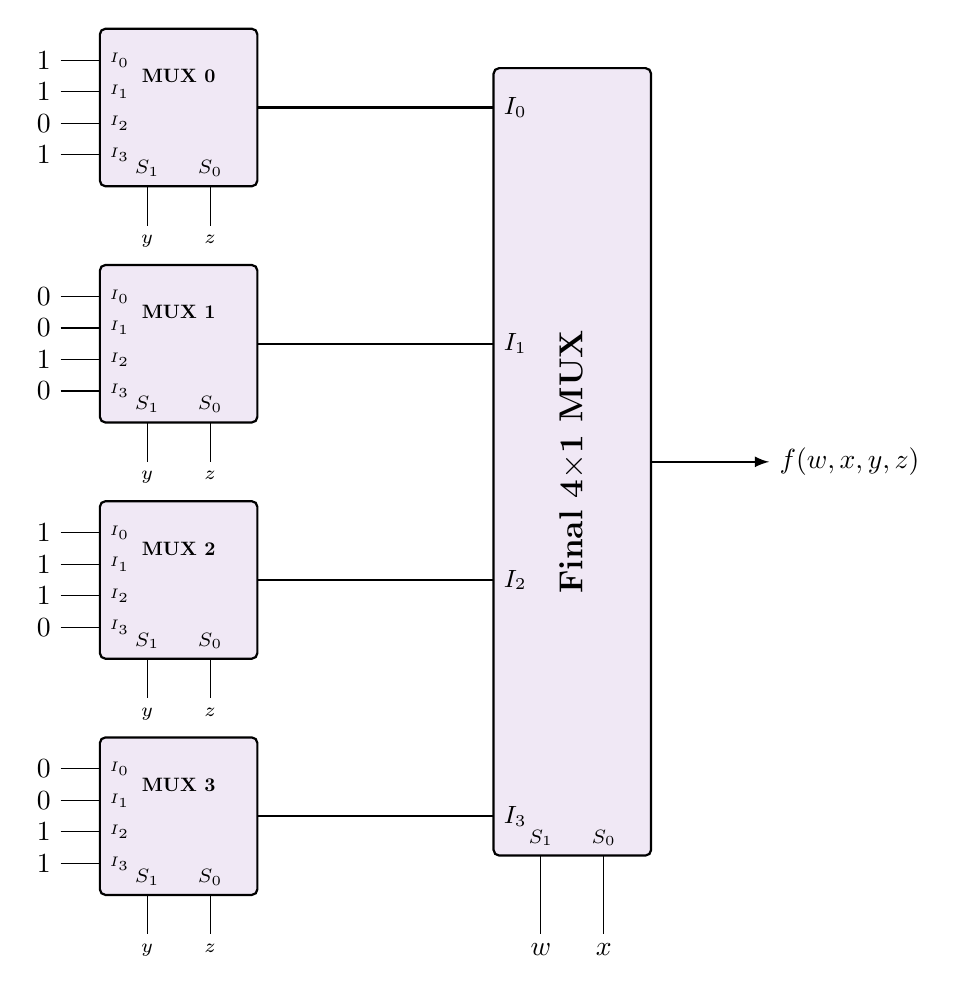
\begin{tikzpicture}[>=latex]

    % --- Level 1 MUXes ---
    % MUX 0
    \draw[thick, fill=cD!10, rounded corners=2pt] (0, 9) rectangle (2, 11);
    \node[scale=0.7] at (1, 10.4) {\textbf{MUX 0}};
    \draw (-0.5, 10.6) node[left] {$1$} -- (0, 10.6) node[right, font=\tiny] {$I_0$};
    \draw (-0.5, 10.2) node[left] {$1$} -- (0, 10.2) node[right, font=\tiny] {$I_1$};
    \draw (-0.5, 9.8) node[left] {$0$} -- (0, 9.8) node[right, font=\tiny] {$I_2$};
    \draw (-0.5, 9.4) node[left] {$1$} -- (0, 9.4) node[right, font=\tiny] {$I_3$};
    \node[above, font=\scriptsize] at (0.6, 9) {$S_1$};
    \node[above, font=\scriptsize] at (1.4, 9) {$S_0$};
    \draw (0.6, 9) -- (0.6, 8.5) node[below, font=\scriptsize] {$y$};
    \draw (1.4, 9) -- (1.4, 8.5) node[below, font=\scriptsize] {$z$};

    % MUX 1
    \draw[thick, fill=cD!10, rounded corners=2pt] (0, 6) rectangle (2, 8);
    \node[scale=0.7] at (1, 7.4) {\textbf{MUX 1}};
    \draw (-0.5, 7.6) node[left] {$0$} -- (0, 7.6) node[right, font=\tiny] {$I_0$};
    \draw (-0.5, 7.2) node[left] {$0$} -- (0, 7.2) node[right, font=\tiny] {$I_1$};
    \draw (-0.5, 6.8) node[left] {$1$} -- (0, 6.8) node[right, font=\tiny] {$I_2$};
    \draw (-0.5, 6.4) node[left] {$0$} -- (0, 6.4) node[right, font=\tiny] {$I_3$};
    \node[above, font=\scriptsize] at (0.6, 6) {$S_1$};
    \node[above, font=\scriptsize] at (1.4, 6) {$S_0$};
    \draw (0.6, 6) -- (0.6, 5.5) node[below, font=\scriptsize] {$y$};
    \draw (1.4, 6) -- (1.4, 5.5) node[below, font=\scriptsize] {$z$};

    % MUX 2
    \draw[thick, fill=cD!10, rounded corners=2pt] (0, 3) rectangle (2, 5);
    \node[scale=0.7] at (1, 4.4) {\textbf{MUX 2}};
    \draw (-0.5, 4.6) node[left] {$1$} -- (0, 4.6) node[right, font=\tiny] {$I_0$};
    \draw (-0.5, 4.2) node[left] {$1$} -- (0, 4.2) node[right, font=\tiny] {$I_1$};
    \draw (-0.5, 3.8) node[left] {$1$} -- (0, 3.8) node[right, font=\tiny] {$I_2$};
    \draw (-0.5, 3.4) node[left] {$0$} -- (0, 3.4) node[right, font=\tiny] {$I_3$};
    \node[above, font=\scriptsize] at (0.6, 3) {$S_1$};
    \node[above, font=\scriptsize] at (1.4, 3) {$S_0$};
    \draw (0.6, 3) -- (0.6, 2.5) node[below, font=\scriptsize] {$y$};
    \draw (1.4, 3) -- (1.4, 2.5) node[below, font=\scriptsize] {$z$};

    % MUX 3
    \draw[thick, fill=cD!10, rounded corners=2pt] (0, 0) rectangle (2, 2);
    \node[scale=0.7] at (1, 1.4) {\textbf{MUX 3}};
    \draw (-0.5, 1.6) node[left] {$0$} -- (0, 1.6) node[right, font=\tiny] {$I_0$};
    \draw (-0.5, 1.2) node[left] {$0$} -- (0, 1.2) node[right, font=\tiny] {$I_1$};
    \draw (-0.5, 0.8) node[left] {$1$} -- (0, 0.8) node[right, font=\tiny] {$I_2$};
    \draw (-0.5, 0.4) node[left] {$1$} -- (0, 0.4) node[right, font=\tiny] {$I_3$};
    \node[above, font=\scriptsize] at (0.6, 0) {$S_1$};
    \node[above, font=\scriptsize] at (1.4, 0) {$S_0$};
    \draw (0.6, 0) -- (0.6, -0.5) node[below, font=\scriptsize] {$y$};
    \draw (1.4, 0) -- (1.4, -0.5) node[below, font=\scriptsize] {$z$};

    % --- Level 2 (Output) MUX ---
    \draw[thick, fill=cD!10, rounded corners=2pt] (5, 0.5) rectangle (7, 10.5);
    \node[rotate=90] at (6, 5.5) {\large \textbf{Final 4$\times$1 MUX}};
    
    % Level 2 Selectors
    \node[above, font=\scriptsize] at (5.6, 0.5) {$S_1$};
    \node[above, font=\scriptsize] at (6.4, 0.5) {$S_0$};
    \draw (5.6, 0.5) -- (5.6, -0.5) node[below] {$w$};
    \draw (6.4, 0.5) -- (6.4, -0.5) node[below] {$x$};

    % Wires from Level 1 to Level 2
    \draw[thick] (2, 10) -- (5, 10) node[right, font=\small] {$I_0$};
    \draw[thick] (2, 7) -- (5, 7) node[right, font=\small] {$I_1$};
    \draw[thick] (2, 4) -- (5, 4) node[right, font=\small] {$I_2$};
    \draw[thick] (2, 1) -- (5, 1) node[right, font=\small] {$I_3$};

    % Final Output
    \draw[thick, ->] (7, 5.5) -- (8.5, 5.5) node[right] {\textbf{$f(w,x,y,z)$}};

\end{tikzpicture}
\end{center}

\end{tcolorbox}

\item Design and implement the circuit diagram of a 1-bit full subtractor circuit using $2\times1$ MUXs only. You cannot use any other gates.
\mk{12} \yr{CSE 205 | L-2/T-1 | 2015--16}

\begin{tcolorbox}[enhanced,breakable,ansbox,colback=cD!4,colframe=cD,boxrule=0.8pt,arc=5pt,title={\textbf{Answer}},fonttitle=\bfseries\color{white},colbacktitle=cD]

\textbf{Step 1: Truth Table of a 1-bit Full Subtractor}

A full subtractor performs the operation $A - B - B_{in}$, producing a Difference ($D$) and a Borrow-out ($B_{out}$). 

\begin{center}
\renewcommand{\arraystretch}{1.2}
\begin{tabular}{ccc|cc}
\toprule
\multicolumn{3}{c|}{\textbf{Inputs}} & \multicolumn{2}{c}{\textbf{Outputs}} \\
$A$ (Minuend) & $B$ (Subtrahend) & $B_{in}$ (Borrow-in) & $D$ (Difference) & $B_{out}$ (Borrow-out) \\
\midrule
$0$ & $0$ & $0$ & $0$ & $0$ \\
$0$ & $0$ & $1$ & $1$ & $1$ \\
$0$ & $1$ & $0$ & $1$ & $1$ \\
$0$ & $1$ & $1$ & $0$ & $1$ \\
\midrule
$1$ & $0$ & $0$ & $1$ & $0$ \\
$1$ & $0$ & $1$ & $0$ & $0$ \\
$1$ & $1$ & $0$ & $0$ & $0$ \\
$1$ & $1$ & $1$ & $1$ & $1$ \\
\bottomrule
\end{tabular}
\end{center}

\textbf{Step 2: Mathematical Derivation using Shannon's Expansion}

To implement these functions using \textbf{only} $2\times1$ multiplexers, we use Shannon's Expansion Theorem to factor the expressions around the variables $A$ and $B$, since a $2\times1$ MUX natively implements the logic $Y = \overline{S}I_0 + SI_1$.

\vspace{0.3cm}
\textbf{1. Difference ($D$):}
\begin{align*}
D(A, B, B_{in}) &= \overline{A} \cdot \left[ \overline{B}(B_{in}) + B(\overline{B_{in}}) \right] + A \cdot \left[ \overline{B}(\overline{B_{in}}) + B(B_{in}) \right]
\end{align*}
This directly implies a 2-level MUX tree:
\begin{itemize}
    \item \textbf{MUX 1} ($A=0$ branch, Selector=$B$): $I_0 = B_{in}$, $I_1 = \overline{B_{in}}$
    \item \textbf{MUX 2} ($A=1$ branch, Selector=$B$): $I_0 = \overline{B_{in}}$, $I_1 = B_{in}$
    \item \textbf{MUX 3} (Output stage, Selector=$A$): $I_0 = \text{MUX 1}_{out}$, $I_1 = \text{MUX 2}_{out}$
\end{itemize}

\vspace{0.2cm}
\textbf{2. Borrow-out ($B_{out}$):}
\begin{align*}
B_{out}(A, B, B_{in}) &= \overline{A} \cdot \left[ \overline{B}(B_{in}) + B(1) \right] + A \cdot \left[ \overline{B}(0) + B(B_{in}) \right]
\end{align*}
Similarly, this gives us:
\begin{itemize}
    \item \textbf{MUX 4} ($A=0$ branch, Selector=$B$): $I_0 = B_{in}$, $I_1 = 1$
    \item \textbf{MUX 5} ($A=1$ branch, Selector=$B$): $I_0 = 0$, $I_1 = B_{in}$
    \item \textbf{MUX 6} (Output stage, Selector=$A$): $I_0 = \text{MUX 4}_{out}$, $I_1 = \text{MUX 5}_{out}$
\end{itemize}

\vspace{0.2cm}
\textbf{3. NOT Gate for $\overline{B_{in}}$:}
Because we cannot use standard logic gates, we must generate $\overline{B_{in}}$ using a $2\times1$ MUX:
\begin{align*}
\overline{B_{in}} &= \overline{B_{in}}\cdot(1) + B_{in}\cdot(0)
\end{align*}
\begin{itemize}
    \item \textbf{MUX 0} (Inverter, Selector=$B_{in}$): $I_0 = 1$, $I_1 = 0$
\end{itemize}

\vspace{0.5cm}
\textbf{Step 3: Circuit Implementation}

\begin{center}
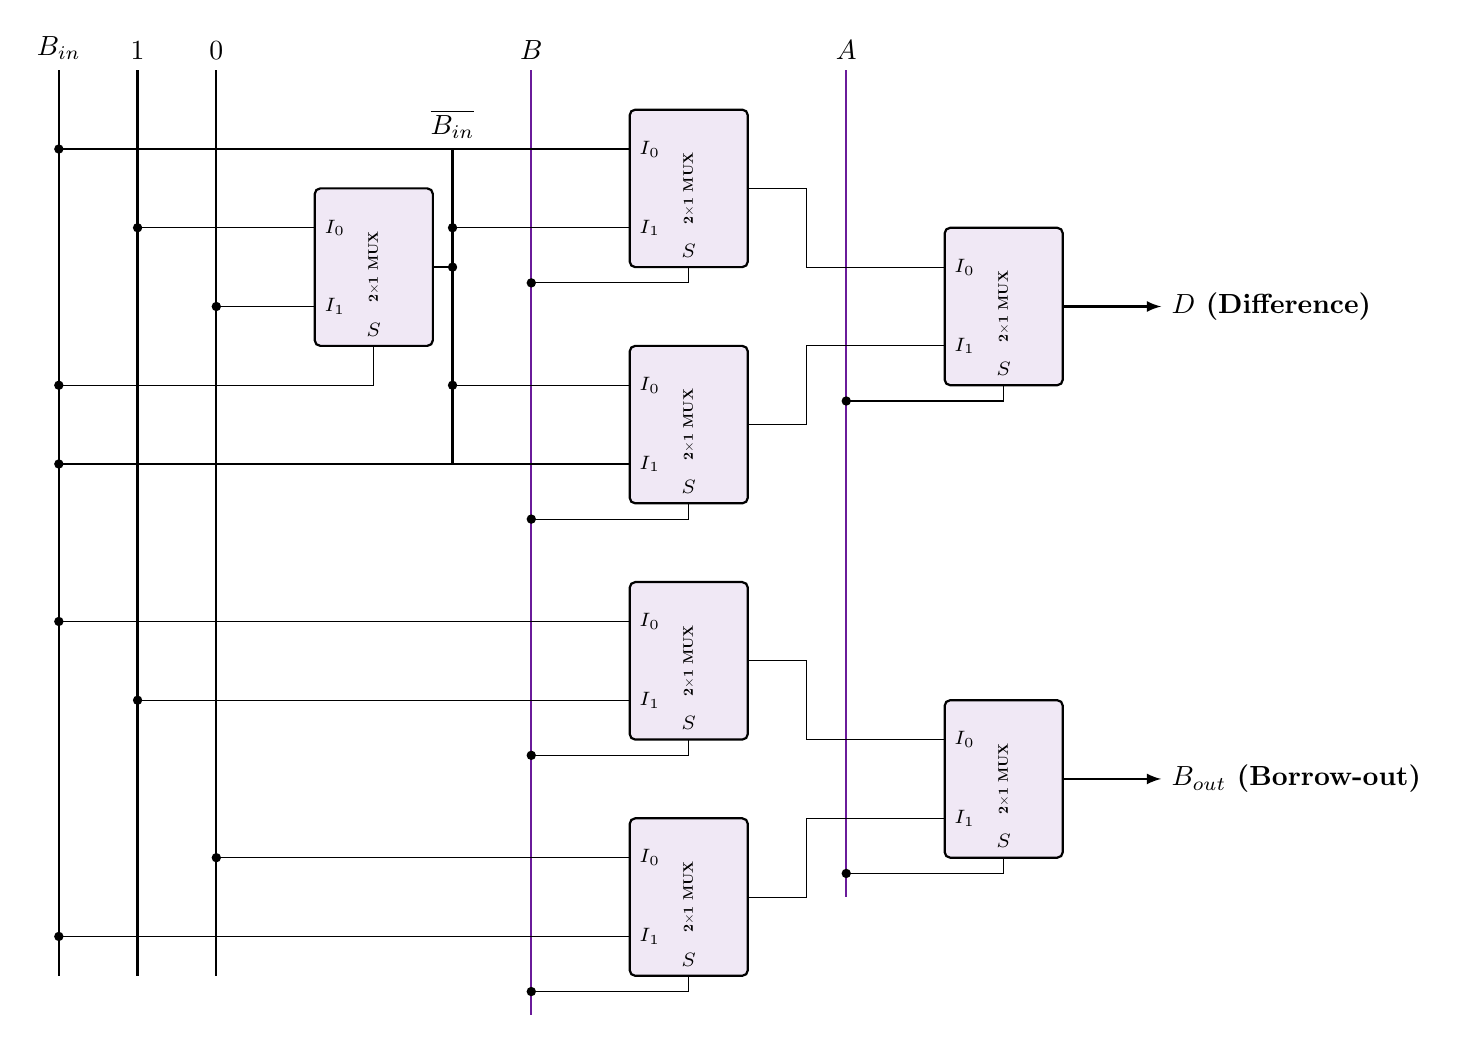
\begin{tikzpicture}[>=latex]

    % --- Data and Control Rails ---
    \draw[thick] (0, 12.5) node[above] {$B_{in}$} -- (0, 1);
    \draw[thick] (1, 12.5) node[above] {$1$} -- (1, 1);
    \draw[thick] (2, 12.5) node[above] {$0$} -- (2, 1);
    \draw[thick, cD] (6, 12.5) node[above, text=black] {$B$} -- (6, 0.5);
    \draw[thick, cD] (10, 12.5) node[above, text=black] {$A$} -- (10, 2);

    % --- Inverter MUX (M0) ---
    \draw[thick, fill=cD!10, rounded corners=2pt] (3.25, 9) rectangle (4.75, 11);
    \node[rotate=90, scale=0.5] at (4, 10) {\textbf{2$\times$1 MUX}};
    \node[right, font=\scriptsize] at (3.25, 10.5) {$I_0$};
    \node[right, font=\scriptsize] at (3.25, 9.5) {$I_1$};
    \node[above, font=\scriptsize] at (4, 9) {$S$};
    
    % M0 Connections
    \draw (1, 10.5) node[circle,fill,inner sep=1.2pt]{} -- (3.25, 10.5); % I0 = 1
    \draw (2, 9.5) node[circle,fill,inner sep=1.2pt]{} -- (3.25, 9.5);   % I1 = 0
    \draw (0, 8.5) node[circle,fill,inner sep=1.2pt]{} -- (4, 8.5) -- (4, 9); % S = Bin
    \draw[thick] (4.75, 10) -- (5, 10) node[circle,fill,inner sep=1.2pt]{};
    \draw[thick] (5, 11.5) node[above] {$\overline{B_{in}}$} -- (5, 7.5); % Bin_bar rail

    % --- MUX Array generation using a loop ---
    % \x, \y, \name
    \foreach \x/\y/\name in {
        8/11/M1,
        8/8/M2,
        8/5/M4,
        8/2/M5,
        12/9.5/M3,
        12/3.5/M6%
    } {
        \draw[thick, fill=cD!10, rounded corners=2pt] (\x-0.75, \y-1) rectangle (\x+0.75, \y+1);
        \node[rotate=90, scale=0.5] at (\x, \y) {\textbf{2$\times$1 MUX}};
        \node[right, font=\scriptsize] at (\x-0.75, \y+0.5) {$I_0$};
        \node[right, font=\scriptsize] at (\x-0.75, \y-0.5) {$I_1$};
        \node[above, font=\scriptsize] at (\x, \y-1) {$S$};
    }

    % --- MUX 1 (D, A=0) ---
    \draw (0, 11.5) node[circle,fill,inner sep=1.2pt]{} -- (7.25, 11.5); % I0 = Bin
    \draw (5, 10.5) node[circle,fill,inner sep=1.2pt]{} -- (7.25, 10.5); % I1 = Bin_bar
    \draw (6, 9.8) node[circle,fill,inner sep=1.2pt]{} -- (8, 9.8) -- (8, 10); % S = B

    % --- MUX 2 (D, A=1) ---
    \draw (5, 8.5) node[circle,fill,inner sep=1.2pt]{} -- (7.25, 8.5);  % I0 = Bin_bar
    \draw (0, 7.5) node[circle,fill,inner sep=1.2pt]{} -- (7.25, 7.5);  % I1 = Bin
    \draw (6, 6.8) node[circle,fill,inner sep=1.2pt]{} -- (8, 6.8) -- (8, 7); % S = B

    % --- MUX 4 (Bout, A=0) ---
    \draw (0, 5.5) node[circle,fill,inner sep=1.2pt]{} -- (7.25, 5.5); % I0 = Bin
    \draw (1, 4.5) node[circle,fill,inner sep=1.2pt]{} -- (7.25, 4.5); % I1 = 1
    \draw (6, 3.8) node[circle,fill,inner sep=1.2pt]{} -- (8, 3.8) -- (8, 4); % S = B

    % --- MUX 5 (Bout, A=1) ---
    \draw (2, 2.5) node[circle,fill,inner sep=1.2pt]{} -- (7.25, 2.5); % I0 = 0
    \draw (0, 1.5) node[circle,fill,inner sep=1.2pt]{} -- (7.25, 1.5); % I1 = Bin
    \draw (6, 0.8) node[circle,fill,inner sep=1.2pt]{} -- (8, 0.8) -- (8, 1); % S = B

    % --- MUX 3 (D Final) ---
    \draw (8.75, 11) -- (9.5, 11) -- (9.5, 10) -- (11.25, 10); % I0 = M1 Out
    \draw (8.75, 8) -- (9.5, 8) -- (9.5, 9) -- (11.25, 9);    % I1 = M2 Out
    \draw (10, 8.3) node[circle,fill,inner sep=1.2pt]{} -- (12, 8.3) -- (12, 8.5); % S = A

    % --- MUX 6 (Bout Final) ---
    \draw (8.75, 5) -- (9.5, 5) -- (9.5, 4) -- (11.25, 4); % I0 = M4 Out
    \draw (8.75, 2) -- (9.5, 2) -- (9.5, 3) -- (11.25, 3); % I1 = M5 Out
    \draw (10, 2.3) node[circle,fill,inner sep=1.2pt]{} -- (12, 2.3) -- (12, 2.5); % S = A

    % --- Outputs ---
    \draw[thick, ->] (12.75, 9.5) -- (14, 9.5) node[right] {\textbf{$D$ (Difference)}};
    \draw[thick, ->] (12.75, 3.5) -- (14, 3.5) node[right] {\textbf{$B_{out}$ (Borrow-out)}};

\end{tikzpicture}
\end{center}

\end{tcolorbox}

\item Consider the Boolean function $f(w, x, y, z) = \Pi\,(2,4,5,7,11,12,13)$. Implement the function using a $4 \times 1$ MUX and other basic gates if necessary.
\mk{10} \yr{CSE 205 | L-2/T-1 | 2015--16}

\begin{tcolorbox}[enhanced,breakable,ansbox,colback=cD!4,colframe=cD,boxrule=0.8pt,arc=5pt,title={\textbf{Answer}},fonttitle=\bfseries\color{white},colbacktitle=cD]

\textbf{Step 1: Convert the Function to Sum of Products (SOP) Form}

The given Boolean function is provided in Product of Sums (POS) form, specifying the maxterms. For a 4-variable function ($w, x, y, z$), the domain ranges from $0$ to $15$. We first convert this to the Sum of Products (SOP) form by identifying the missing indices, which correspond to the minterms:
\begin{align*}
f(w, x, y, z) &= \prod M(2, 4, 5, 7, 11, 12, 13) \\
              &= \sum m(0, 1, 3, 6, 8, 9, 10, 14, 15)
\end{align*}

\textbf{Step 2: Assign Variables to the Multiplexer Selectors}

We are required to implement the function using a $4 \times 1$ multiplexer. A $4 \times 1$ MUX requires exactly $2$ selector lines ($S_1, S_0$). 
We will assign the two Most Significant Bits (MSBs) to the selector lines:
\begin{itemize}
    \item $S_1 = w$
    \item $S_0 = x$
\end{itemize}
This implies that the multiplexer's data inputs ($I_0, I_1, I_2, I_3$) will be derived as Boolean expressions in terms of the remaining variables, $y$ and $z$.

\vspace{0.3cm}
\textbf{Step 3: Deriving MUX Data Inputs}

We evaluate the minterms corresponding to each selector combination to find the expressions for $I_0, I_1, I_2, I_3$.

\textbf{1. For $w=0, x=0$ (Selects $I_0$):}
This branch covers minterms $m_0, m_1, m_2, m_3$. The minterms present in the function are $m_0, m_1, m_3$.
\begin{align*}
    I_0(y, z) &= \bar{y}\bar{z} + \bar{y}z + yz \\
              &= \bar{y}(\bar{z} + z) + yz \quad &&\text{(Factoring out } \bar{y} \text{)} \\
              &= \bar{y}(1) + yz \quad &&\text{(Complement Law: } \bar{z} + z = 1 \text{)} \\
              &= \bar{y} + yz \\
              &= (\bar{y} + y)(\bar{y} + z) \quad &&\text{(Distributive Law)} \\
              &= \bar{y} + z
\end{align*}

\textbf{2. For $w=0, x=1$ (Selects $I_1$):}
This branch covers minterms $m_4, m_5, m_6, m_7$. The only minterm present is $m_6$.
\begin{align*}
    I_1(y, z) &= y\bar{z}
\end{align*}

\textbf{3. For $w=1, x=0$ (Selects $I_2$):}
This branch covers minterms $m_8, m_9, m_{10}, m_{11}$. The minterms present are $m_8, m_9, m_{10}$.
\begin{align*}
    I_2(y, z) &= \bar{y}\bar{z} + \bar{y}z + y\bar{z} \\
              &= \bar{y}(\bar{z} + z) + y\bar{z} \\
              &= \bar{y} + y\bar{z} \\
              &= (\bar{y} + y)(\bar{y} + \bar{z}) \quad &&\text{(Distributive Law)} \\
              &= \bar{y} + \bar{z} \\
              &= \overline{yz} \quad &&\text{(De Morgan's Law)}
\end{align*}

\textbf{4. For $w=1, x=1$ (Selects $I_3$):}
This branch covers minterms $m_{12}, m_{13}, m_{14}, m_{15}$. The minterms present are $m_{14}, m_{15}$.
\begin{align*}
    I_3(y, z) &= y\bar{z} + yz \\
              &= y(\bar{z} + z) \\
              &= y
\end{align*}

\textbf{Summary of Inputs:}
\begin{center}
\renewcommand{\arraystretch}{1.2}
\begin{tabular}{cc|c|l}
\toprule
$w$ ($S_1$) & $x$ ($S_0$) & \textbf{Active Minterms ($y, z$)} & \textbf{Input Equation} \\
\midrule
$0$ & $0$ & $m_0, m_1, m_3$ & $I_0 = \bar{y} + z$ \\
$0$ & $1$ & $m_6$ & $I_1 = y\bar{z}$ \\
$1$ & $0$ & $m_8, m_9, m_{10}$ & $I_2 = \overline{yz}$ \\
$1$ & $1$ & $m_{14}, m_{15}$ & $I_3 = y$ \\
\bottomrule
\end{tabular}
\end{center}

\vspace{0.5cm}
\textbf{Step 4: Circuit Diagram}

The logical expressions for the inputs can be implemented using standard basic gates: an OR gate for $I_0$, an AND gate for $I_1$, and a NAND gate for $I_2$ (implementing $\bar{y} + \bar{z}$ directly via De Morgan's theorem). Inverters are used to generate $\bar{y}$ and $\bar{z}$.

\vspace{0.5cm}
\begin{center}
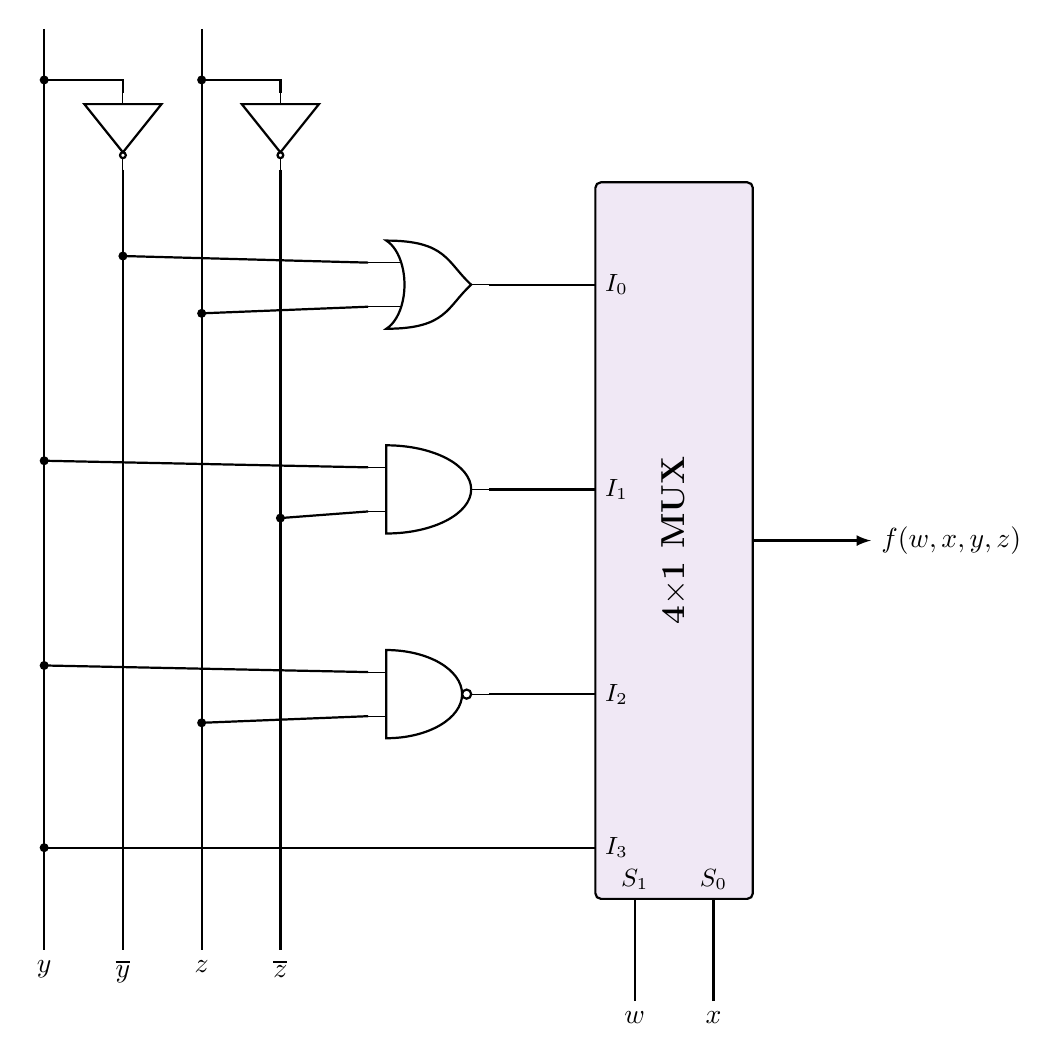
\begin{tikzpicture}[>=latex, y=1.3cm]

    % --- Data Rails ---
    % y and y_bar rails
    \draw[thick] (-3, 9) -- (-3, 0) node[below] {$y$};
    \node[not port, rotate=-90, scale=0.7] (noty) at (-2, 8) {};
    \draw[thick, fill=black] (-3, 8.5) circle (1.2pt);
    \draw[thick] (-3, 8.5) -- (-2, 8.5) -- (noty.in);
    \draw[thick] (noty.out) -- (-2, 0) node[below] {$\overline{y}$};

    % z and z_bar rails
    \draw[thick] (-1, 9) -- (-1, 0) node[below] {$z$};
    \node[not port, rotate=-90, scale=0.7] (notz) at (0, 8) {};
    \draw[thick, fill=black] (-1, 8.5) circle (1.2pt);
    \draw[thick] (-1, 8.5) -- (0, 8.5) -- (notz.in);
    \draw[thick] (notz.out) -- (0, 0) node[below] {$\overline{z}$};

    % --- 4x1 Multiplexer ---
    \draw[thick, fill=cD!10, rounded corners=2pt] (4, 0.5) rectangle (6, 7.5);
    \node[rotate=90] at (5, 4) {\large \textbf{4$\times$1 MUX}};
    
    % MUX Input Labels
    \node[right, font=\small] at (4, 6.5) {$I_0$};
    \node[right, font=\small] at (4, 4.5) {$I_1$};
    \node[right, font=\small] at (4, 2.5) {$I_2$};
    \node[right, font=\small] at (4, 1.0) {$I_3$};
    
    % Selector Labels
    \node[above, font=\small] at (4.5, 0.5) {$S_1$};
    \node[above, font=\small] at (5.5, 0.5) {$S_0$};

    % Selector Pins
    \draw[thick] (4.5, -0.5) node[below] {$w$} -- (4.5, 0.5);
    \draw[thick] (5.5, -0.5) node[below] {$x$} -- (5.5, 0.5);

    % --- Logic Gates & Wiring ---

    % I0 = y_bar + z (OR Gate)
    \node[or port] (or1) at (2.5, 6.5) {};
    \draw[thick, fill=black] (-2, 6.78) circle (1.2pt);
    \draw[thick] (-2, 6.78) -- (or1.in 1);
    \draw[thick, fill=black] (-1, 6.22) circle (1.2pt);
    \draw[thick] (-1, 6.22) -- (or1.in 2);
    \draw[thick] (or1.out) -- (4, 6.5);

    % I1 = y * z_bar (AND Gate)
    \node[and port] (and1) at (2.5, 4.5) {};
    \draw[thick, fill=black] (-3, 4.78) circle (1.2pt);
    \draw[thick] (-3, 4.78) -- (and1.in 1);
    \draw[thick, fill=black] (0, 4.22) circle (1.2pt);
    \draw[thick] (0, 4.22) -- (and1.in 2);
    \draw[thick] (and1.out) -- (4, 4.5);

    % I2 = (yz)_bar (NAND Gate implementing y_bar + z_bar)
    \node[nand port] (nand1) at (2.5, 2.5) {};
    \draw[thick, fill=black] (-3, 2.78) circle (1.2pt);
    \draw[thick] (-3, 2.78) -- (nand1.in 1);
    \draw[thick, fill=black] (-1, 2.22) circle (1.2pt);
    \draw[thick] (-1, 2.22) -- (nand1.in 2);
    \draw[thick] (nand1.out) -- (4, 2.5);

    % I3 = y (Direct connection)
    \draw[thick, fill=black] (-3, 1.0) circle (1.2pt);
    \draw[thick] (-3, 1.0) -- (4, 1.0);

    % --- Final Output ---
    \draw[thick, ->] (6, 4) -- (7.5, 4) node[right] {\textbf{$f(w,x,y,z)$}};

\end{tikzpicture}
\end{center}


\end{tcolorbox}

\item Show the truth table for a three-state buffer. Construct a 2-to-1 line MUX with three-state buffers.
\mk{3+5} \yr{CSE 205 | L-2/T-1 | 2014--15}

\begin{tcolorbox}[enhanced,breakable,ansbox,colback=cD!4,colframe=cD,boxrule=0.8pt,arc=5pt,title={\textbf{Answer}},fonttitle=\bfseries\color{white},colbacktitle=cD]

\subsection*{1. Truth Table for a Three-State Buffer}
A three-state (or tri-state) buffer acts as a standard buffer but includes a third operational state: \textbf{High-Impedance ($Z$)}. It is controlled by an Enable line ($E$). 
\begin{itemize}
    \item When $E = 1$ (Active), the buffer acts normally, passing the input $A$ directly to the output $Y$.
    \item When $E = 0$ (Inactive), the output is disconnected from the input, placing the output in a High-Impedance state ($Z$), effectively acting as an open circuit.
\end{itemize}

\begin{center}
\renewcommand{\arraystretch}{1.3}
\begin{tabular}{cc | c}
\toprule
\multicolumn{2}{c|}{\textbf{Inputs}} & \textbf{Output} \\
\textbf{Enable ($E$)} & \textbf{Data ($A$)} & \textbf{$Y$} \\
\midrule
0 & X (Don't Care) & \textcolor{cD}{\textbf{Z}} (High-Impedance) \\
1 & 0 & \textbf{0} \\
1 & 1 & \textbf{1} \\
\bottomrule
\end{tabular}
\end{center}

\vspace{0.4cm}
\subsection*{2. Construction of a 2-to-1 MUX using Three-State Buffers}

A 2-to-1 Multiplexer routes one of two input signals ($I_0$ or $I_1$) to a single output ($Y$) based on the value of a Select line ($S$).
Using three-state buffers, we can construct this by connecting the outputs of two buffers together. To avoid bus contention (short circuits), we must ensure that \textbf{only one buffer is enabled at any given time}.

\begin{itemize}
    \item \textbf{When $S = 0$:} The inverted signal $\overline{S} = 1$ enables the top buffer. Input $I_0$ is passed to $Y$. The bottom buffer is in state $Z$.
    \item \textbf{When $S = 1$:} The direct signal $S = 1$ enables the bottom buffer. Input $I_1$ is passed to $Y$. The top buffer is in state $Z$.
\end{itemize}

\begin{center}
\begin{circuitikz}[scale=1.2, transform shape, thick]
    
    % Select Line S
    \draw (-2, 0) node[left, font=\bfseries] {$S$} -- (-1, 0);
    \fill (-1, 0) circle (2pt);
    
    % Inverter for Select Line
    \node[not port, scale=0.7, fill=cD!10, draw=cD] (inv) at (0.5, 3) {};
    \draw (-1, 0) |- (inv.in);
    
    % Tri-state Buffers
    \node[buffer port, fill=cD!10, draw=cD] (buf0) at (3, 1.5) {};
    \node[buffer port, fill=cD!10, draw=cD] (buf1) at (3, -1.5) {};
    
    % Enable logic routing
    % Route inverted S to top buffer's enable (top edge of the bounding box)
    \draw (inv.out) -| (buf0.north);
    
    % Route direct S to bottom buffer's enable (bottom edge of the bounding box)
    \draw (-1, 0) |- (1.5, -3) -| (buf1.south);
    
    % Data Inputs
    \draw (0, 1.5) node[left, font=\bfseries] {$I_0$} -- (buf0.in);
    \draw (0, -1.5) node[left, font=\bfseries] {$I_1$} -- (buf1.in);
    
    % Common Output Junction
    \draw (buf0.out) -| (4.5, 0);
    \draw (buf1.out) -| (4.5, 0);
    \fill (4.5, 0) circle (2pt);
    
    % Final Output Y
    \draw[->, draw=cD] (4.5, 0) -- (5.5, 0) node[right, font=\bfseries, text=cD] {$Y$};

\end{circuitikz}
\end{center}

\end{tcolorbox}

\item An $8 \times 1$ multiplexer has inputs $A, B, C, D$ where inputs $A$, $B$, and $C$ are connected to selection inputs $S_2$, $S_1$, and $S_0$ respectively. The data inputs $I_0$ through $I_7$ are: $I_1 = I_2 = 0$; $I_3 = I_7 = 1$; $I_4 = I_5 = D$; $I_0 = I_6 = D'$. Determine the Boolean function that the multiplexer implements.
\mk{15} \yr{CSE 205 | L-2/T-1 | 2013--14}

\begin{tcolorbox}[enhanced,breakable,ansbox,colback=cD!4,colframe=cD,boxrule=0.8pt,arc=5pt,title={\textbf{Answer}},fonttitle=\bfseries\color{white},colbacktitle=cD]

\subsection*{1. Characteristic Equation of the $8 \times 1$ Multiplexer}
An $8 \times 1$ multiplexer outputs a Boolean function determined by the logical sum of the products of its selection line minterms and their corresponding data inputs. The general output equation $F$ is given by:
\[ F(S_2, S_1, S_0) = \sum_{k=0}^{7} m_k \cdot I_k \]
where $m_k$ represents the $k$-th minterm of the selection variables. 

Given the selection inputs $S_2 = A$, $S_1 = B$, and $S_0 = C$, we can map the given data inputs $I_0$ through $I_7$ as follows:

\begin{center}
\renewcommand{\arraystretch}{1.3}
\begin{tabular}{ccc | c | c}
\toprule
\multicolumn{3}{c|}{\textbf{Selection Lines}} & \textbf{Data Input} & \textbf{Assigned Value} \\
$A \ (S_2)$ & $B \ (S_1)$ & $C \ (S_0)$ & $I_k$ & $F(A,B,C,D)$ \\
\midrule
0 & 0 & 0 & $I_0$ & $D'$ \\
0 & 0 & 1 & $I_1$ & $0$ \\
0 & 1 & 0 & $I_2$ & $0$ \\
0 & 1 & 1 & $I_3$ & $1$ \\
1 & 0 & 0 & $I_4$ & $D$ \\
1 & 0 & 1 & $I_5$ & $D$ \\
1 & 1 & 0 & $I_6$ & $D'$ \\
1 & 1 & 1 & $I_7$ & $1$ \\
\bottomrule
\end{tabular}
\end{center}

\vspace{0.2cm}
\subsection*{2. Algebraic Formulation}
Substituting the given data inputs into the characteristic equation:
\begin{align*}
    F(A,B,C,D) &= A'B'C'(D') + A'B'C(0) + A'BC'(0) + A'BC(1) \\
               &\quad + AB'C'(D) + AB'C(D) + ABC'(D') + ABC(1) \\[8pt]
    &= A'B'C'D' + 0 + 0 + A'BC + AB'C'D + AB'CD + ABC'D' + ABC \\
    &= A'B'C'D' + A'BC + AB'C'D + AB'CD + ABC'D' + ABC
\end{align*}

\vspace{0.2cm}
\subsection*{3. Conversion to Canonical Sum of Minterms (SOP)}
To find the standard minterms $\Sigma m$, we expand the terms missing the variable $D$ by multiplying them by $(D + D') = 1$ (Complement Law):
\begin{align*}
    A'BC &= A'BC(D + D') = A'BCD + A'BCD' \quad &&(\text{Minterms } 7, 6) \\
    ABC &= ABC(D + D') = ABCD + ABCD' \quad &&(\text{Minterms } 15, 14)
\end{align*}
The remaining terms are already standard minterms:
\begin{itemize}
    \item $A'B'C'D' \rightarrow m_0$
    \item $AB'C'D \rightarrow m_9$
    \item $AB'CD \rightarrow m_{11}$
    \item $ABC'D' \rightarrow m_{12}$
\end{itemize}
Thus, the canonical Boolean function implemented by the multiplexer is:
\[ \textcolor{cD}{\mathbf{F(A,B,C,D) = \Sigma m(0, 6, 7, 9, 11, 12, 14, 15)}} \]

\vspace{0.2cm}
\subsection*{4. Logic Minimization using Karnaugh Map}
We map the active minterms onto a 4-variable K-map to determine the simplified Boolean expression.

\begin{center}
\begin{karnaugh-map}[4][4][1][$CD$][$AB$]
    \minterms{0,6,7,9,11,12,14,15}
    \autoterms[0]
    % Group 1: 2x2 Square (6, 7, 14, 15) -> BC
    \implicant{7}{14}
    % Group 2: Horizontal Pair (9, 11) -> AB'D
    \implicant{9}{11}
    % Group 3: Edge Pair (12, 14) -> ABD'
    \implicantedge{12}{12}{14}{14}
    % Group 4: Isolated Minterm (0) -> A'B'C'D'
    \implicant{0}{0}
\end{karnaugh-map}
\end{center}

\textbf{Group Extractions:}
\begin{itemize}
    \item \textbf{Red / $2 \times 2$ Block ($m_6, m_7, m_{14}, m_{15}$):} Variables $A$ and $D$ change, leaving $\mathbf{BC}$.
    \item \textbf{Green / Horizontal Pair ($m_9, m_{11}$):} Variable $C$ changes, leaving $\mathbf{AB'D}$.
    \item \textbf{Blue / Edge Pair ($m_{12}, m_{14}$):} Variable $C$ changes, leaving $\mathbf{ABD'}$.
    \item \textbf{Yellow / Isolated Cell ($m_0$):} No variables change, leaving $\mathbf{A'B'C'D'}$.
\end{itemize}

\vspace{0.2cm}
\textbf{Final Minimal Boolean Function:}
\begin{align*}
    \textcolor{cD}{\mathbf{F(A,B,C,D) = BC + AB'D + ABD' + A'B'C'D'}}
\end{align*}

\end{tcolorbox}

\item Construct a $16 \times 1$ multiplexer with two $8 \times 1$ and one $2 \times 1$ multiplexers.
\mk{5} \yr{CSE 205 | L-2/T-1 | 2013--14}

\begin{tcolorbox}[enhanced,breakable,ansbox,colback=cD!4,colframe=cD,boxrule=0.8pt,arc=5pt,title={\textbf{Answer}},fonttitle=\bfseries\color{white},colbacktitle=cD]

\subsection*{1. Design Strategy and Logic Formulation}
A $16 \times 1$ multiplexer routes one of $16$ data inputs ($I_0$ to $I_{15}$) to a single output ($Y$) based on a 4-bit selection code ($S_3, S_2, S_1, S_0$), where $S_3$ is the Most Significant Bit (MSB).

Since we have $8 \times 1$ multiplexers available (which accept 3 selection bits and 8 data inputs), we can partition the 16 inputs into two groups of 8:
\begin{itemize}
    \item \textbf{Lower Half ($I_0$ to $I_7$):} Selected when the MSB $S_3 = 0$.
    \item \textbf{Upper Half ($I_8$ to $I_{15}$):} Selected when the MSB $S_3 = 1$.
\end{itemize}

\textbf{Configuration Step-by-Step:}
\begin{enumerate}
    \item \textbf{First Stage ($8 \times 1$ Multiplexers):} 
    The three Least Significant Bits (LSBs) $S_2, S_1, S_0$ are applied simultaneously to the selection lines of both $8 \times 1$ multiplexers. 
    \begin{align*}
        F_1 &= \Sigma_{k=0}^{7} m_k(S_2, S_1, S_0) \cdot I_k \quad &&\text{(Output of top MUX)} \\
        F_2 &= \Sigma_{k=0}^{7} m_k(S_2, S_1, S_0) \cdot I_{k+8} \quad &&\text{(Output of bottom MUX)}
    \end{align*}
    
    \item \textbf{Second Stage ($2 \times 1$ Multiplexer):}
    The outputs $F_1$ and $F_2$ serve as the data inputs to the $2 \times 1$ multiplexer. The MSB $S_3$ acts as the selection line for this final multiplexer to toggle between the lower and upper data banks.
    \begin{align*}
        Y &= \overline{S_3} \cdot F_1 + S_3 \cdot F_2 \quad &&\text{(Multiplexer logical expansion)}
    \end{align*}
\end{enumerate}

\vspace{0.4cm}
\subsection*{2. Truth Table Summary}
\begin{center}
\renewcommand{\arraystretch}{1.2}
\begin{tabular}{c | ccc | c | c}
\toprule
\multicolumn{4}{c|}{\textbf{Selection Lines}} & \textbf{Active MUX} & \textbf{Selected Output ($Y$)} \\
$S_3$ & $S_2$ & $S_1$ & $S_0$ & \textbf{in 1st Stage} & \\
\midrule
0 & 0 & 0 & 0 & \multirow{2}{*}{MUX 1 (Top)} & $I_0$ \\
$\vdots$ & $\vdots$ & $\vdots$ & $\vdots$ & & $\vdots$ \\
0 & 1 & 1 & 1 & & $I_7$ \\
\midrule
1 & 0 & 0 & 0 & \multirow{2}{*}{MUX 2 (Bottom)} & $I_8$ \\
$\vdots$ & $\vdots$ & $\vdots$ & $\vdots$ & & $\vdots$ \\
1 & 1 & 1 & 1 & & $I_{15}$ \\
\bottomrule
\end{tabular}
\end{center}

\vspace{0.4cm}
\subsection*{3. Logic Circuit Implementation}

\begin{center}
\begin{circuitikz}[scale=0.9, transform shape, thick]
    
    % ================= First Stage: 8x1 MUX 1 (Top) =================
    \draw[fill=white, rounded corners=2pt] (0, 3) rectangle (3, 9);
    \node[align=center, font=\bfseries] at (1.5, 6) {8-to-1 \\ MUX 1};
    
    % MUX 1 Data Inputs
    \foreach \i in {0,...,7} {
        \pgfmathsetmacro{\y}{8.4 - \i*0.7}
        \draw[<-] (0, \y) -- (-1.5, \y) node[left, font=\bfseries] {$I_{\i}$};
    }
    
    % ================= First Stage: 8x1 MUX 2 (Bottom) =================
    \draw[fill=white, rounded corners=2pt] (0, -5) rectangle (3, 1);
    \node[align=center, font=\bfseries] at (1.5, -2) {8-to-1 \\ MUX 2};

    % MUX 2 Data Inputs
    \foreach \i in {8,...,15} {
        \pgfmathsetmacro{\idx}{\i - 8}
        \pgfmathsetmacro{\y}{0.4 - \idx*0.7}
        \draw[<-] (0, \y) -- (-1.5, \y) node[left, font=\bfseries] {$I_{\i}$};
    }

    % ================= Second Stage: 2x1 MUX 3 (Right) =================
    \draw[fill=white, rounded corners=2pt] (6, 0.5) rectangle (8.5, 3.5);
    \node[align=center, font=\bfseries] at (7.25, 2) {2-to-1 \\ MUX 3};
    
    % MUX 3 Data Labels
    \node[right, font=\small\bfseries] at (6, 2.5) {0};
    \node[right, font=\small\bfseries] at (6, 1.5) {1};

    % ================= Data Routing =================
    % MUX 1 to MUX 3 (Input 0)
    \draw[->] (3, 6) -- (5.5, 6) |- (6, 2.5);
    % MUX 2 to MUX 3 (Input 1)
    \draw[->] (3, -2) -- (5.5, -2) |- (6, 1.5);
    
    % Final Output Y
    \draw[->, thick] (8.5, 2) -- (10, 2) node[right, font=\bfseries] {$Y$};

    % ================= Shared Selection Lines Bus =================
    % S3 Routing (MUX 3)
    \draw (-1.5, -6) node[left, font=\bfseries] {$S_3$ (MSB)} -- (7.25, -6) -- (7.25, 0.5);
    \node[above, font=\small\bfseries] at (7.25, 0.5) {$S_3$};

    % S2 Routing
    \draw (-1.5, -6.5) node[left, font=\bfseries] {$S_2$} -- (4.5, -6.5) -- (4.5, 2.5) -- (1, 2.5) -- (1, 3);
    \draw (1, -6.5) -- (1, -5);
    \fill (1, -6.5) circle (2pt);
    
    % S1 Routing
    \draw (-1.5, -7) node[left, font=\bfseries] {$S_1$} -- (4.0, -7) -- (4.0, 2.0) -- (1.5, 2.0) -- (1.5, 3);
    \draw (1.5, -7) -- (1.5, -5);
    \fill (1.5, -7) circle (2pt);
    
    % S0 Routing
    \draw (-1.5, -7.5) node[left, font=\bfseries] {$S_0$ (LSB)} -- (3.5, -7.5) -- (3.5, 1.5) -- (2, 1.5) -- (2, 3);
    \draw (2, -7.5) -- (2, -5);
    \fill (2, -7.5) circle (2pt);

    % ================= Select Line Internal Labels =================
    % MUX 1 Selection Labels
    \node[above, font=\small\bfseries] at (1, 3) {$S_2$};
    \node[above, font=\small\bfseries] at (1.5, 3) {$S_1$};
    \node[above, font=\small\bfseries] at (2, 3) {$S_0$};

    % MUX 2 Selection Labels
    \node[above, font=\small\bfseries] at (1, -5) {$S_2$};
    \node[above, font=\small\bfseries] at (1.5, -5) {$S_1$};
    \node[above, font=\small\bfseries] at (2, -5) {$S_0$};

\end{circuitikz}
\end{center}

\end{tcolorbox}

\item Implement $F = \Sigma\,(3,5,7,10,11,13,14,15)$ using a 16-to-1 MUX.
\mk{10} \yr{CSE 205 | L-2/T-1 | 2012--13}

\begin{tcolorbox}[enhanced,breakable,ansbox,colback=cD!4,colframe=cD,boxrule=0.8pt,arc=5pt,title={\textbf{Answer}},fonttitle=\bfseries\color{white},colbacktitle=cD]

\subsection*{1. MUX Implementation Strategy}
A 16-to-1 Multiplexer has 4 selection lines ($S_3, S_2, S_1, S_0$) and 16 data inputs ($I_0$ to $I_{15}$). 
To implement a 4-variable Boolean function $F(A,B,C,D)$ directly using a 16-to-1 MUX, we follow a straightforward mapping technique:
\begin{itemize}
    \item Connect the 4 Boolean variables directly to the 4 selection lines: $S_3 = A$, $S_2 = B$, $S_1 = C$, and $S_0 = D$.
    \item Connect the data inputs $I_i$ corresponding to the active minterms (present in the function) to \textbf{Logic 1} ($V_{cc}$).
    \item Connect the data inputs $I_i$ corresponding to the absent minterms to \textbf{Logic 0} (Ground).
\end{itemize}

Given the function:
\[ F(A,B,C,D) = \Sigma\,(3,5,7,10,11,13,14,15) \]
The active minterms are $m_3, m_5, m_7, m_{10}, m_{11}, m_{13}, m_{14}, m_{15}$.

\vspace{0.2cm}
\subsection*{2. Input Mapping Table}
\begin{center}
\renewcommand{\arraystretch}{1.2}
\begin{tabular}{c | cccc | c | l}
\toprule
\textbf{Minterm} & \textbf{$A (S_3)$} & \textbf{$B (S_2)$} & \textbf{$C (S_1)$} & \textbf{$D (S_0)$} & \textbf{Data Input} & \textbf{Assigned Value} \\
\midrule
$m_0, m_1, m_2$ & \multicolumn{4}{c|}{Various combinations} & $I_0, I_1, I_2$ & \textbf{0} (GND) \\
$m_3$ & 0 & 0 & 1 & 1 & $I_3$ & \textcolor{cD}{\textbf{1}} ($V_{cc}$) \\
$m_4$ & 0 & 1 & 0 & 0 & $I_4$ & \textbf{0} (GND) \\
$m_5$ & 0 & 1 & 0 & 1 & $I_5$ & \textcolor{cD}{\textbf{1}} ($V_{cc}$) \\
$m_6$ & 0 & 1 & 1 & 0 & $I_6$ & \textbf{0} (GND) \\
$m_7$ & 0 & 1 & 1 & 1 & $I_7$ & \textcolor{cD}{\textbf{1}} ($V_{cc}$) \\
$m_8, m_9$ & \multicolumn{4}{c|}{Various combinations} & $I_8, I_9$ & \textbf{0} (GND) \\
$m_{10}, m_{11}$ & \multicolumn{4}{c|}{Various combinations} & $I_{10}, I_{11}$ & \textcolor{cD}{\textbf{1}} ($V_{cc}$) \\
$m_{12}$ & 1 & 1 & 0 & 0 & $I_{12}$ & \textbf{0} (GND) \\
$m_{13}, m_{14}, m_{15}$ & \multicolumn{4}{c|}{Various combinations} & $I_{13}, I_{14}, I_{15}$ & \textcolor{cD}{\textbf{1}} ($V_{cc}$) \\
\bottomrule
\end{tabular}
\end{center}

\vspace{0.4cm}
\subsection*{3. Circuit Diagram}

\begin{center}
\begin{circuitikz}[scale=1.1, transform shape, thick]
    
    % Draw the 16-to-1 MUX Block
    \draw[fill=white, rounded corners=2pt] (0, 0) rectangle (3, 9);
    \node[align=center, font=\bfseries] at (1.5, 4.5) {16-to-1 \\ MUX};

    % Draw Logic 1 and Logic 0 buses
    \draw (-2.5, 9) node[above, font=\bfseries, text=cD, scale=0.5] {Logic 1 ($V_{cc}$)} -- (-2.5, 0.5);
    \draw (-1.2, 9) -- (-1.2, 0.5);
    \node[above, font=\bfseries, scale=0.5]  at (-0.5, 9) {Logic 0 (GND)};

    % Inputs mapped to Logic 1: {3, 5, 7, 10, 11, 13, 14, 15}
    \foreach \i in {3, 5, 7, 10, 11, 13, 14, 15} {
        \pgfmathsetmacro{\y}{8.6 - \i*0.5}
        \draw[draw=cD] (-2.5, \y) -- (0, \y);
        \fill[cD] (-2.5, \y) circle (2pt);
        \node[right, font=\small\bfseries] at (0, \y) {$I_{\i}$};
    }

    % Inputs mapped to Logic 0: {0, 1, 2, 4, 6, 8, 9, 12}
    \foreach \i in {0, 1, 2, 4, 6, 8, 9, 12} {
        \pgfmathsetmacro{\y}{8.6 - \i*0.5}
        \draw (-1.2, \y) -- (0, \y);
        \fill (-1.2, \y) circle (2pt);
        \node[right, font=\small\bfseries] at (0, \y) {$I_{\i}$};
    }

    % Selection Lines
    \draw[<-] (0.6, 0) -- (0.6, -1) node[below, font=\bfseries, scale=0.5] {$S_3 \ (A)$};
    \draw[<-] (1.2, 0) -- (1.2, -1) node[below, font=\bfseries, scale=0.5] {$S_2 \ (B)$};
    \draw[<-] (1.8, 0) -- (1.8, -1) node[below, font=\bfseries, scale=0.5] {$S_1 \ (C)$};
    \draw[<-] (2.4, 0) -- (2.4, -1) node[below, font=\bfseries, scale=0.5] {$S_0 \ (D)$};

    % Output Line
    \draw[->, draw=cD] (3, 4.5) -- (4.5, 4.5) node[right, font=\bfseries, text=cD] {$F(A,B,C,D)$};

\end{circuitikz}
\end{center}

\end{tcolorbox}

\item Can the function $F = \Sigma\,(3,5,7,10,11,13,14,15)$ be implemented using only one $4 \times 1$ MUX? If yes, show how; if not, explain why.
\mk{10} \yr{CSE 205 | L-2/T-1 | 2012--13}

\begin{tcolorbox}[enhanced,breakable,ansbox,colback=cD!4,colframe=cD,boxrule=0.8pt,arc=5pt,title={\textbf{Answer}},fonttitle=\bfseries\color{white},colbacktitle=cD]

\textbf{Conclusion:} 
Yes, the function $F(A,B,C,D) = \Sigma\,(3,5,7,10,11,13,14,15)$ \textbf{can} be implemented using strictly one $4 \times 1$ multiplexer (MUX) and absolutely no additional logic gates. This is achieved by strategically choosing variables $C$ and $D$ as the selection lines.

\vspace{1em}
\textbf{\large 1. Theoretical Foundation}

A $4 \times 1$ MUX implements any logic function conforming to its characteristic equation:
\begin{align*}
    Y &= S_1'S_0' I_0 + S_1'S_0 I_1 + S_1S_0' I_2 + S_1S_0 I_3
\end{align*}
where $S_1, S_0$ are the select lines and $I_0, I_1, I_2, I_3$ are the data inputs. 

To implement a 4-variable function using only one $4 \times 1$ MUX (which has 2 select lines), we must map two variables to the select lines. The remaining two variables will dictate the logic required at the data inputs. To avoid using external logic gates (such as AND/OR/NOT gates), the data inputs must resolve entirely to constants ($0$ or $1$) or single input variables (uncomplemented or complemented). 

\vspace{1em}
\textbf{\large 2. Mathematical Derivation (Shannon's Expansion)}

We apply Shannon's Expansion Theorem to factor out the variables $C$ and $D$, setting them as our select variables ($S_1 = C$, $S_0 = D$). 

First, let us expand the given function into its canonical sum of minterms:
\begin{align*}
F(A,B,C,D) &= \sum m(3,5,7,10,11,13,14,15) \\
&= m_3 + m_5 + m_7 + m_{10} + m_{11} + m_{13} + m_{14} + m_{15} \\
&= A'B'CD + A'BC'D + A'BCD + AB'CD' + AB'CD + ABC'D + ABCD' + ABCD
\end{align*}

Next, we group the terms based on the four possible combinations of $C$ and $D$:
\begin{align*}
F &= C'D'(0) && \text{(No minterms end in $C=0, D=0$)} \\
  &\quad + C'D\,(A'B + AB) && \text{(From $m_5$ and $m_{13}$)} \\
  &\quad + CD'\,(AB' + AB) && \text{(From $m_{10}$ and $m_{14}$)} \\
  &\quad + CD\,(A'B' + A'B + AB' + AB) && \text{(From $m_3, m_7, m_{11}, m_{15}$)}
\end{align*}

Now, we systematically simplify the expressions for each MUX input using Boolean algebra:

\begin{itemize}
    \item \textbf{For $C'D'$ ($I_0$):} \\
    The coefficient is $0$. \\
    $\therefore \textcolor{cD}{\mathbf{I_0 = 0}}$

    \item \textbf{For $C'D$ ($I_1$):} \\
    \begin{align*}
    I_1 &= A'B + AB \\
        &= B(A' + A) \quad &&\text{(Distributive Law)} \\
        &= B(1) \quad &&\text{(Complement Law: $A' + A = 1$)} \\
        \therefore \textcolor{cD}{\mathbf{I_1}} &\textcolor{cD}{\mathbf{= B}} \quad &&\text{(Identity Law)}
    \end{align*}

    \item \textbf{For $CD'$ ($I_2$):} \\
    \begin{align*}
    I_2 &= AB' + AB \\
        &= A(B' + B) \quad &&\text{(Distributive Law)} \\
        &= A(1) \quad &&\text{(Complement Law: $B' + B = 1$)} \\
        \therefore \textcolor{cD}{\mathbf{I_2}} &\textcolor{cD}{\mathbf{= A}} \quad &&\text{(Identity Law)}
    \end{align*}

    \item \textbf{For $CD$ ($I_3$):} \\
    \begin{align*}
    I_3 &= A'B' + A'B + AB' + AB \\
        &= A'(B' + B) + A(B' + B) \quad &&\text{(Distributive Law)} \\
        &= A'(1) + A(1) \quad &&\text{(Complement Law)} \\
        &= A' + A \quad &&\text{(Identity Law)} \\
        \therefore \textcolor{cD}{\mathbf{I_3}} &\textcolor{cD}{\mathbf{= 1}} \quad &&\text{(Complement Law)}
    \end{align*}
\end{itemize}

Since all derived inputs ($0$, $B$, $A$, and $1$) can be obtained via direct wiring without any logic gates, the implementation is valid.

\vspace{1em}
\textbf{\large 3. Implementation Table}

The following table maps the state of the select lines ($C, D$) to the corresponding minterms and the necessary data inputs.

\begin{center}
\renewcommand{\arraystretch}{1.3}
\begin{tabular}{ccclc}
\toprule
\textbf{$S_1$ ($C$)} & \textbf{$S_0$ ($D$)} & \textbf{Data Input} & \textbf{Relevant Minterms in $F$} & \textbf{Simplified Input} \\
\midrule
0 & 0 & $I_0$ & None & $\mathbf{0}$ \\
0 & 1 & $I_1$ & $m_5 (0101), m_{13} (1101)$ & $\mathbf{B}$ \\
1 & 0 & $I_2$ & $m_{10} (1010), m_{14} (1110)$ & $\mathbf{A}$ \\
1 & 1 & $I_3$ & $m_3 (0011), m_7 (0111), m_{11} (1011), m_{15} (1111)$ & $\mathbf{1}$ \\
\bottomrule
\end{tabular}
\end{center}

\vspace{1em}
\textbf{\large 4. Circuit Diagram}

\begin{center}
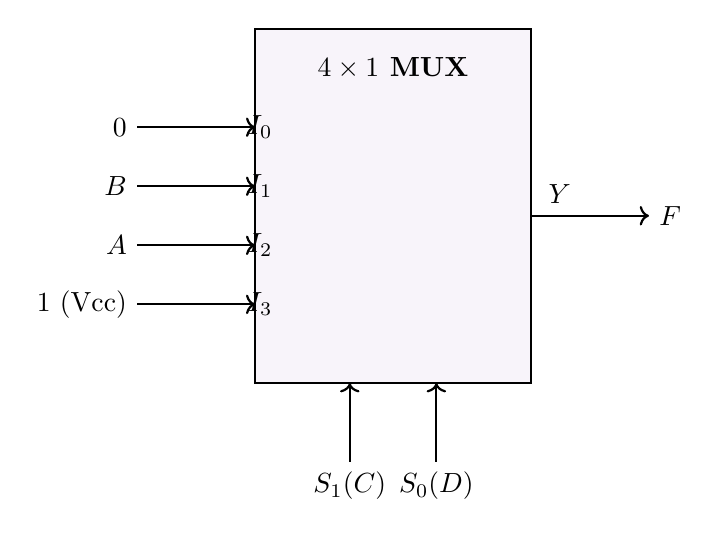
\begin{tikzpicture}
    % MUX Block
    \draw[thick, fill=cD!5] (0,0) rectangle (3.5,4.5);
    \node at (1.75, 4) {\textbf{$4 \times 1$ MUX}};
    
    % Data Inputs
    \draw[->, thick] (-1.5, 3.25) -- (0, 3.25) node[pos=0, left] {$0$} node[pos=0.85, right] {$I_0$};
    \draw[->, thick] (-1.5, 2.5) -- (0, 2.5) node[pos=0, left] {$B$} node[pos=0.85, right] {$I_1$};
    \draw[->, thick] (-1.5, 1.75) -- (0, 1.75) node[pos=0, left] {$A$} node[pos=0.85, right] {$I_2$};
    \draw[->, thick] (-1.5, 1.0) -- (0, 1.0) node[pos=0, left] {$1$ (Vcc)} node[pos=0.85, right] {$I_3$};
    
    % Select Lines
    \draw[->, thick] (1.2, -1) -- (1.2, 0) node[pos=0, below] {$S_1 (C)$};
    \draw[->, thick] (2.3, -1) -- (2.3, 0) node[pos=0, below] {$S_0 (D)$};
    
    % Output
    \draw[->, thick] (3.5, 2.125) -- (5, 2.125) node[pos=1, right] {$F$};
    \node[right] at (3.6, 2.4) {$Y$};
\end{tikzpicture}
\end{center}

\textit{Note: If we had chosen $A$ and $B$ as the select lines instead, the inputs $I_0$ through $I_3$ would have required complex expressions in terms of $C$ and $D$ (e.g., $I_3 = C+D$), which would necessitate additional logic gates. The choice of $C$ and $D$ perfectly avoids this constraint.}

\end{tcolorbox}

\item Implement the following function $F$ using one $4 \times 1$ multiplexer and basic gates:
\[ F(A,B,C,D) = \Sigma\,(1,3,4,11,12,13,14,15) \]
\mk{15} \yr{CSE 205 | L-2/T-1 | 2011--12}

\begin{tcolorbox}[enhanced,breakable,ansbox,colback=cD!4,colframe=cD,boxrule=0.8pt,arc=5pt,title={\textbf{Answer}},fonttitle=\bfseries\color{white},colbacktitle=cD]

\textbf{1. Multiplexer Sizing and Variable Selection}

To implement a 4-variable Boolean function $F(A,B,C,D)$ using a $4 \times 1$ Multiplexer (MUX), we need to allocate the variables strategically. 
A $4 \times 1$ MUX has:
\begin{itemize}
    \item $4$ data inputs ($I_0, I_1, I_2, I_3$)
    \item $2$ select lines ($S_1, S_0$)
\end{itemize}
We will connect the two most significant variables, $A$ and $B$, to the select lines:
\[ S_1 = A, \quad S_0 = B \]
The remaining variables, $C$ and $D$, will be used to generate the data inputs $I_0, I_1, I_2, \text{ and } I_3$.

\vspace{0.5cm}
\textbf{2. Implementation Table}

We map the given minterms $\Sigma\,(1,3,4,11,12,13,14,15)$ into an implementation table based on the permutations of $C$ and $D$ for each combination of $A$ and $B$. Minterms present in the function are highlighted in \textbf{\textcolor{cD}{bold}}.

\begin{center}
\renewcommand{\arraystretch}{1.4}
\begin{tabular}{@{}lcccc@{}}
\toprule
\textbf{Data Variables} & $\mathbf{I_0}$ & $\mathbf{I_1}$ & $\mathbf{I_2}$ & $\mathbf{I_3}$ \\
\textbf{Select ($AB$)} & \textbf{($00$)} & \textbf{($01$)} & \textbf{($10$)} & \textbf{($11$)} \\
\midrule
$\bar{C}\bar{D} \ (00)$ & $0$ & \textbf{\textcolor{cD}{4}} & $8$ & \textbf{\textcolor{cD}{12}} \\
$\bar{C}D \ (01)$       & \textbf{\textcolor{cD}{1}} & $5$ & $9$ & \textbf{\textcolor{cD}{13}} \\
$C\bar{D} \ (10)$       & $2$ & $6$ & $10$ & \textbf{\textcolor{cD}{14}} \\
$CD \ (11)$             & \textbf{\textcolor{cD}{3}} & $7$ & \textbf{\textcolor{cD}{11}} & \textbf{\textcolor{cD}{15}} \\
\midrule
\textbf{Boolean Sum} & $I_0 = \bar{C}D + CD$ & $I_1 = \bar{C}\bar{D}$ & $I_2 = CD$ & $I_3 = \bar{C}\bar{D} + \bar{C}D + C\bar{D} + CD$ \\
\bottomrule
\end{tabular}
\end{center}

\vspace{0.5cm}
\textbf{3. Mathematical Derivation of Data Inputs}

We simplify the logic expressions for each data input using fundamental Boolean algebra laws:

\begin{align*}
I_0 &= \bar{C}D + CD \\
    &= D(\bar{C} + C) && \text{(Distributive Law)} \\
    &= D(1) && \text{(Complementarity Law: } X + \bar{X} = 1 \text{)} \\
    &= D && \text{(Identity Law)} \\[10pt]
I_1 &= \bar{C}\bar{D} && \text{(No further simplification needed)} \\[10pt]
I_2 &= CD && \text{(No further simplification needed)} \\[10pt]
I_3 &= \bar{C}\bar{D} + \bar{C}D + C\bar{D} + CD \\
    &= \bar{C}(\bar{D} + D) + C(\bar{D} + D) && \text{(Distributive Law)} \\
    &= \bar{C}(1) + C(1) && \text{(Complementarity Law)} \\
    &= \bar{C} + C \\
    &= 1 && \text{(Complementarity Law)}
\end{align*}

\vspace{0.2cm}
\textbf{Summary of MUX Inputs:}
\begin{itemize}
    \item $I_0 = D$
    \item $I_1 = \bar{C}\bar{D}$ (Implemented using an AND gate with inverted inputs)
    \item $I_2 = CD$ (Implemented using an AND gate)
    \item $I_3 = 1$ (Connected to Logic HIGH / $+V_{CC}$)
\end{itemize}

\vspace{0.5cm}
\textbf{4. Logic Circuit Diagram}

Below is the complete hardware implementation using standard basic logic gates and the $4 \times 1$ MUX block:

\begin{center}
\begin{circuitikz}[thick, scale=1.1, transform shape]
    
    % MUX Box Outline
    \draw[fill=white] (0,0) rectangle (3,6);
    \node at (1.5, 3) {\large \textbf{4$\times$1 MUX}};

    % Select Lines
    \draw (1, -1) node[below, scale=0.5] {$S_1 = A$} -- (1, 0);
    \draw (2, -1) node[below, scale=0.5] {$S_0 = B$} -- (2, 0);

    % Output Line
    \draw (3, 3) -- (4, 3) node[right] {\textbf{$F$}};

    % MUX Input Pin Labels
    \node[right] at (0, 5) {$I_0$};
    \node[right] at (0, 3.8) {$I_1$};
    \node[right] at (0, 2.2) {$I_2$};
    \node[right] at (0, 1) {$I_3$};

    % Small connecting wires to the MUX boundary
    \draw (-0.5, 5) -- (0, 5);
    \draw (-0.5, 3.8) -- (0, 3.8);
    \draw (-0.5, 2.2) -- (0, 2.2);
    \draw (-0.5, 1) -- (0, 1);

    % Input Variable Rails (C and D)
    \draw (-6.5, 6.5) -- (-6.5, 0) node[below] {$C$};
    \draw (-5.5, 6.5) -- (-5.5, 0) node[below] {$D$};

    % --- I0 = D ---
    \draw (-5.5, 5) node[circ]{} -- (-0.5, 5);

    % --- I1 = C'D' ---
    % AND gate for I1
    \node[and port, scale=0.8] (andI1) at (-2, 3.8) {};
    \draw (andI1.out) -- (-0.5, 3.8);
    
    % NOT gates for I1 inputs
    \node[not port, scale=0.4] (notC) at ([xshift=-1.5cm]andI1.in 1) {};
    \node[not port, scale=0.4] (notD) at ([xshift=-1.5cm]andI1.in 2) {};
    
    \draw (notC.out) -- (andI1.in 1);
    \draw (notD.out) -- (andI1.in 2);
    
    % Connections from Rails to NOT gates
    \draw (-6.5, 0 |- notC.in) node[circ]{} -- (notC.in);
    \draw (-5.5, 0 |- notD.in) node[circ]{} -- (notD.in);

    % --- I2 = CD ---
    % AND gate for I2
    \node[and port, scale=0.8] (andI2) at (-2, 2.2) {};
    \draw (andI2.out) -- (-0.5, 2.2);

    % Connections from Rails directly to AND gate
    \draw (-6.5, 0 |- andI2.in 1) node[circ]{} -- (andI2.in 1);
    \draw (-5.5, 0 |- andI2.in 2) node[circ]{} -- (andI2.in 2);

    % --- I3 = 1 ---
    \node[left] at (-0.5, 1) {\textbf{Logic 1} ($+V_{CC}$)};

\end{circuitikz}
\end{center}

\end{tcolorbox}
\end{enumerate}

%%──────────────────────────────────────────────────────────────────────
\subtopic{cD}{Custom Combinational Circuit Design}
\label{sub:s4-comb-custom}

\begin{enumerate}

\item Using a 4-bit binary adder and XOR gates, design a circuit which takes two 4-bit BCD inputs $A$ and $B$ and returns: $A+1$ if input is 00; $A'$ if input is 01; $A'+1$ if input is 10; $A$ if input is 11.
\mk{13} \yr{CSE 205 | L-2/T-1 | 2018--19}

\begin{tcolorbox}[enhanced,breakable,ansbox,colback=cD!4,colframe=cD,boxrule=0.8pt,arc=5pt,title={\textbf{Answer}},fonttitle=\bfseries\color{white},colbacktitle=cD]

\textbf{1. Problem Analysis \& Interpretation}

The problem requires designing an arithmetic logic circuit using only a \textbf{4-bit binary adder} and \textbf{XOR gates}. We are given a 4-bit data input $A$. 
\textit{Note on Input B:} While the problem description mentions $B$ as a 4-bit BCD input, the operational modes provided (00, 01, 10, 11) correspond to a 2-bit control space. Therefore, we interpret that the two least significant bits of $B$ (let us denote them as $B_1$ and $B_0$) act as the control inputs to select the operation performed on $A$. 

A standard 4-bit binary adder computes the function:
\[
F = X + Y + C_{in}
\]
where $X$ and $Y$ are 4-bit data inputs, $C_{in}$ is the carry-in bit, and $F$ is the 4-bit sum. Our objective is to determine the appropriate signals for $X$, $Y$, and $C_{in}$ using only $A$, $B_1$, $B_0$, and XOR gates to satisfy the four conditions.

\vspace{0.5cm}
\textbf{2. Target Operations and Adder Input Mapping}

Let us map the desired outputs to the adder's parameters. To either pass $A$ directly or invert it ($A'$), we can use the fundamental property of the XOR gate: 
\[ A \oplus 0 = A \quad \text{and} \quad A \oplus 1 = A' \]
We can fix the second adder input to zero ($Y = 0$). We introduce a control signal $C_X$ such that $X = A \oplus C_X$.

\begin{center}
\renewcommand{\arraystretch}{1.3}
\begin{tabular}{cc|c|ccc}
\toprule
\multicolumn{2}{c|}{\textbf{Control Input}} & \textbf{Desired} & \multicolumn{3}{c}{\textbf{Required Adder Inputs}} \\
$\mathbf{B_1}$ & $\mathbf{B_0}$ & \textbf{Output ($F$)} & $\mathbf{X}$ (Data) & $\mathbf{Y}$ (Data) & $\mathbf{C_{in}}$ (Carry) \\
\midrule
0 & 0 & $A + 1$  & $A$  \ (\text{so } $C_X=0$) & 0 & 1 \\
0 & 1 & $A'$     & $A'$ \ (\text{so } $C_X=1$) & 0 & 0 \\
1 & 0 & $A' + 1$ & $A'$ \ (\text{so } $C_X=1$) & 0 & 1 \\
1 & 1 & $A$      & $A$  \ (\text{so } $C_X=0$) & 0 & 0 \\
\bottomrule
\end{tabular}
\end{center}

\vspace{0.5cm}
\textbf{3. Boolean Derivation for Control Signals}

From the table above, we extract the boolean expressions for $C_X$ and $C_{in}$ in terms of $B_1$ and $B_0$:

\begin{itemize}
    \item \textbf{Deriving $\mathbf{C_{in}}$:} 
    Observing the $C_{in}$ column, the values are $\{1, 0, 1, 0\}$ corresponding to $B_0 = \{0, 1, 0, 1\}$. 
    \[ C_{in} = \overline{B_0} \]
    Since we are constrained to use \textit{only} XOR gates, we can synthesize a NOT gate by XORing with Logic 1 ($V_{CC}$):
    \begin{align*}
        C_{in} &= B_0 \oplus 1
    \end{align*}

    \item \textbf{Deriving $\mathbf{C_X}$:} 
    Observing the required $C_X$ values, we have $C_X = \{0, 1, 1, 0\}$. This is the exact truth table for an XOR operation between $B_1$ and $B_0$.
    \begin{align*}
        C_X &= B_1 \oplus B_0
    \end{align*}
\end{itemize}

Thus, the inputs to the 4-bit adder will be:
\begin{align*}
    X_i &= A_i \oplus C_X = A_i \oplus (B_1 \oplus B_0) \quad \text{for } i \in \{0,1,2,3\} \\
    Y_i &= 0 \quad \text{(Grounded)} \\
    C_{in} &= B_0 \oplus 1
\end{align*}

\vspace{0.5cm}
\textbf{4. Circuit Implementation}

The full schematic utilizes one 4-bit binary adder block and six XOR gates (four for the data path, two for the control logic). Net labels (\textcolor{cD}{\textbf{$C_X$}} and \textcolor{cD}{\textbf{$C_{in}$}}) are utilized for clean routing.

\begin{center}
\begin{circuitikz}[thick]
    % ---------------------------------------------------------
    % Main Adder Block
    % ---------------------------------------------------------
    \draw[fill=cD!5, rounded corners=2pt, draw=cD] (0, 0) rectangle (4, 6);
    \node[align=center, font=\bfseries] at (2, 3) {4-bit \\ Binary \\ Adder};
    
    % Cin and Cout
    \node[below, font=\small] at (2, 6) {$C_{in}$};
    \draw[cD, thick] (2, 6) -- (2, 7) node[above, font=\bfseries] {$C_{in}$};
    
    \node[above, font=\small] at (2, 0) {$C_{out}$};
    \draw (2, 0) -- (2, -1) node[below] {$C_{out}$};

    % ---------------------------------------------------------
    % Data Inputs and XOR Gates
    % ---------------------------------------------------------
    \foreach \i/\y in {3/4.8, 2/3.6, 1/2.4, 0/1.2} {
        % Adder X_i input label
        \node[right, font=\small] at (0, \y) {$X_\i$};
        
        % XOR gates for A_i
        \node[xor port, scale=0.8] (xor\i) at (-2, \y) {};
        
        % Connect XOR to Adder X_i
        \draw (xor\i.out) -- (0, \y);
        
        % A_i inputs
        \draw (xor\i.in 1) -- ++(-2.5, 0) node[left] {$A_\i$};
        
        % C_X connection point (to vertical bus)
        \draw (xor\i.in 2) -- ++(-0.5, 0) coordinate (cx\i);
    }
    
    % Common C_X vertical bus
    \draw[cD, thick] (cx3) -- (cx0);
    \draw[cD, thick] (cx0) -- ++(0, -0.6) node[below, font=\bfseries] {$C_X$};
    \fill[cD] (cx3) circle (1.5pt);
    \fill[cD] (cx2) circle (1.5pt);
    \fill[cD] (cx1) circle (1.5pt);
    \fill[cD] (cx0) circle (1.5pt);

    % Y Inputs (Grounded)
    \node[right, font=\small] at (0, 0.5) {$Y_{3..0}$};
    \draw (0, 0.5) -- (-1.5, 0.5) node[left, font=\bfseries, scale=0.5] {Logic 0 (GND)};

    % Final Sum Outputs (F_i)
    \foreach \i/\y in {3/4.8, 2/3.6, 1/2.4, 0/1.2} {
        \node[left, font=\small] at (4, \y) {$\Sigma_\i$};
        \draw (4, \y) -- (5, \y) node[right, font=\bfseries] {$F_\i$};
    }

    % ---------------------------------------------------------
    % Control Logic Block
    % ---------------------------------------------------------
    \begin{scope}[yshift=-7.5cm, xshift=-1cm]
        % Dashed bounding box
        \draw[dashed, draw=gray, rounded corners=5pt] (1.5, 0) rectangle (7.5, 4);
        \node[font=\bfseries, text=cD] at (4.5, 3.5) {Control Signal Generation};
        
        % Logic Gates
        \node[xor port, scale=0.8] (xorCx) at (5, 2.5) {};
        \node[xor port, scale=0.8] (xorCin) at (5, 1) {};
        
        % Input Connections
        \draw (xorCx.in 1) -- (2.5, 2.724) node[left] {$B_1$};
        \draw (xorCin.in 2) -- (2.5, 0.776) node[left] {Logic 1 ($V_{CC}$)};
        
        % B0 Split Routing (Placed precisely to avoid overlaps)
        \draw (2.5, 1.75) node[left] {$B_0$} -- (3.5, 1.75) coordinate (b0_split);
        \draw (b0_split) |- (xorCx.in 2);
        \draw (b0_split) |- (xorCin.in 1);
        \fill (b0_split) circle (1.5pt);
        
        % Outputs
        \draw[cD, thick] (xorCx.out) -- ++(1,0) node[right, font=\bfseries] {$C_X$};
        \draw[cD, thick] (xorCin.out) -- ++(1,0) node[right, font=\bfseries] {$C_{in}$};
    \end{scope}

\end{circuitikz}
\end{center}
\end{tcolorbox}

\item Design a Binary-to-Excess-3 converter using a logic circuit block with inputs $A$, $B$, $C$, $D$, control lines $x_1$, $x_0$, and active-low $\overline{EN}$. Output~$Y$: if $x_1x_0=00$, $A \to Y$; if $01$, $B \to Y$; if $10$, $C \to Y$; if $11$, $D \to Y$.

\begin{center}
  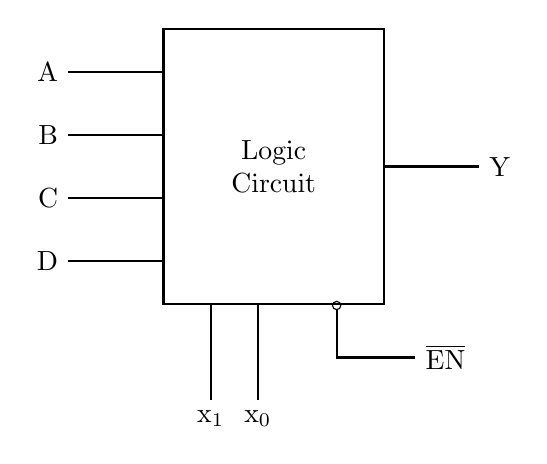
\begin{tikzpicture}[>=latex, font=\normalsize]

  % কেন্দ্রবিন্দু লজিক বক্স (Logic Circuit Box)
  \node [draw, rectangle, minimum height=3.5cm, minimum width=2.8cm, align=center, thick] (box) {
    Logic \\ Circuit
  };

  % --- ইনপুটসমূহ (বাম পাশে) ---
  % বাম ফেসের সাথে কানেকশন পয়েন্টগুলো ডিফাইন করা
  \coordinate (in1) at ([yshift=1.2cm]box.west);
  \coordinate (in2) at ([yshift=0.4cm]box.west);
  \coordinate (in3) at ([yshift=-0.4cm]box.west);
  \coordinate (in4) at ([yshift=-1.2cm]box.west);
  
  % ইনপুট টেক্সট নোট বসানো এবং তার টানা
  \node (A) [left=1.2cm of in1, anchor=east] {A}; \draw [thick] (A.east) -- (in1);
  \node (B) [left=1.2cm of in2, anchor=east] {B}; \draw [thick] (B.east) -- (in2);
  \node (C) [left=1.2cm of in3, anchor=east] {C}; \draw [thick] (C.east) -- (in3);
  \node (D) [left=1.2cm of in4, anchor=east] {D}; \draw [thick] (D.east) -- (in4);

  % --- আউটপুট (ডান পাশে) ---
  \node (Y) [right=1.2cm of box.east, anchor=west] {Y};
  \draw [thick] (box.east) -- (Y.west);

  % --- সিলেক্ট ইনপুটসমূহ (নিচে বাম পাশে) ---
  \coordinate (sel1) at ([xshift=-0.8cm]box.south);
  \coordinate (sel0) at ([xshift=-0.2cm]box.south);
  
  \draw [thick] (sel1) -- ++(0, -1.2cm) node [below] {x\textsubscript{1}};
  \draw [thick] (sel0) -- ++(0, -1.2cm) node [below] {x\textsubscript{0}};

  % --- এনেবল ইনপুট (নিচে ডান পাশে, একটিভ লো বাবল সহ) ---
  % বাবলটি (ছোট বৃত্ত) ঠিক নিচের লাইনের উপর বসানো
  \node [draw, circle, inner sep=0pt, minimum size=3pt] (bubble) at ([xshift=0.8cm]box.south) {};
  
  % বাবল থেকে তার টানা এবং এনেবল লেবেল বসানো
  \draw [thick] (bubble.south) |- ++(1.0cm, -0.6cm) node [right] {$\overline{\text{EN}}$};

\end{tikzpicture}
\end{center}
\mk{8} \yr{CSE 205 | L-2/T-1 | 2016--17}

\begin{tcolorbox}[enhanced,breakable,ansbox,colback=cD!4,colframe=cD,boxrule=0.8pt,arc=5pt,title={\textbf{Answer}},fonttitle=\bfseries\color{white},colbacktitle=cD]

\textbf{1. Component Analysis \& Problem Formulation}

The given logic circuit block functions as a \textbf{4-to-1 Multiplexer (MUX)} with an active-low enable ($\overline{\text{EN}}$). 
\begin{itemize}
    \item \textbf{Data Inputs}: $A, B, C, D$ correspond to select line conditions $x_1x_0 = 00, 01, 10, 11$ respectively.
    \item \textbf{Select Inputs}: $x_1, x_0$ determine which data input is routed to output $Y$.
    \item \textbf{Enable Input}: $\overline{\text{EN}}$ must be tied to Logic 0 (Ground) for normal operation.
\end{itemize}

To design a \textbf{4-bit Binary-to-Excess-3 Converter}, we require four such blocks—one for each output bit of the Excess-3 code ($E_3, E_2, E_1, E_0$). We map the Binary Coded Decimal (BCD) input bits $B_3, B_2, B_1, B_0$ as follows:
\begin{itemize}
    \item We connect the two most significant bits to the select lines of all blocks: $x_1 = B_3$ and $x_0 = B_2$.
    \item The block inputs $A, B, C, D$ for each bit will be derived as Boolean functions of the remaining least significant bits: $B_1$ and $B_0$.
\end{itemize}

\vspace{0.3cm}
\textbf{2. Truth Table \& Input Derivation}

Excess-3 is formed by adding 3 ($0011_2$) to a valid BCD input ($0$ to $9$). The input states $10$ to $15$ are invalid in BCD and are treated as \textbf{Don't Cares (X)} to simplify our hardware logic.

\begin{center}
\renewcommand{\arraystretch}{1.2}
\begin{tabular}{@{}cccc|cccc@{}}
\toprule
\multicolumn{4}{c|}{\textbf{BCD Input}} & \multicolumn{4}{c}{\textbf{Excess-3 Output}} \\
$B_3 (x_1)$ & $B_2 (x_0)$ & $B_1$ & $B_0$ & $E_3$ & $E_2$ & $E_1$ & $E_0$ \\
\midrule
0 & 0 & 0 & 0 & 0 & 0 & 1 & 1 \\
0 & 0 & 0 & 1 & 0 & 1 & 0 & 0 \\
0 & 0 & 1 & 0 & 0 & 1 & 0 & 1 \\
0 & 0 & 1 & 1 & 0 & 1 & 1 & 0 \\
\midrule
0 & 1 & 0 & 0 & 0 & 1 & 1 & 1 \\
0 & 1 & 0 & 1 & 1 & 0 & 0 & 0 \\
0 & 1 & 1 & 0 & 1 & 0 & 0 & 1 \\
0 & 1 & 1 & 1 & 1 & 0 & 1 & 0 \\
\midrule
1 & 0 & 0 & 0 & 1 & 0 & 1 & 1 \\
1 & 0 & 0 & 1 & 1 & 1 & 0 & 0 \\
1 & 0 & 1 & 0 & X & X & X & X \\
1 & 0 & 1 & 1 & X & X & X & X \\
\midrule
1 & 1 & X & X & X & X & X & X \\
\bottomrule
\end{tabular}
\end{center}

By grouping the truth table based on the select lines ($B_3 B_2$), we inspect the behavior of each output with respect to $B_1$ and $B_0$:

\begin{itemize}
    \item \textbf{For $\mathbf{E_0}$:} The pattern is alternating ($1, 0, 1, 0$) for all valid segments. This directly evaluates to the NOT function: \textcolor{cD}{$\mathbf{\overline{B_0}}$}.
    \item \textbf{For $\mathbf{E_1}$:} The pattern is symmetric ($1, 0, 0, 1$) for valid segments. This matches the XNOR function: \textcolor{cD}{$\mathbf{\overline{B_1 \oplus B_0}}$}.
    \item \textbf{For $\mathbf{E_2}$:} 
    \begin{itemize}
        \item When $00$, output is $(0, 1, 1, 1) \implies \text{OR function: } \textcolor{cD}{\mathbf{B_1 + B_0}}$
        \item When $01$, output is $(1, 0, 0, 0) \implies \text{NOR function: } \textcolor{cD}{\mathbf{\overline{B_1 + B_0}}}$
        \item When $10$, valid outputs are $(0, 1)$, matching directly to \textcolor{cD}{$\mathbf{B_0}$}. 
    \end{itemize}
    \item \textbf{For $\mathbf{E_3}$:} 
    \begin{itemize}
        \item When $00$, output is always $(0, 0, 0, 0) \implies \text{Logic } \textcolor{cD}{\mathbf{0}}$
        \item When $01$, output is $(0, 1, 1, 1) \implies \text{OR function: } \textcolor{cD}{\mathbf{B_1 + B_0}}$
        \item When $10$, valid outputs are $(1, 1) \implies \text{Logic } \textcolor{cD}{\mathbf{1}}$
    \end{itemize}
\end{itemize}

Mapping the Don't Care states optimally to reuse existing signals, we formulate the final wiring table for our Logic Blocks:

\begin{center}
\renewcommand{\arraystretch}{1.4}
\begin{tabular}{@{}cc|cccc@{}}
\toprule
\textbf{MUX Input} & \textbf{Select ($B_3 B_2$)} & \textbf{$E_3$ Block} & \textbf{$E_2$ Block} & \textbf{$E_1$ Block} & \textbf{$E_0$ Block} \\
\midrule
$A$ & 00 & $0$ & $B_1+B_0$ & $\overline{B_1 \oplus B_0}$ & $\overline{B_0}$ \\
$B$ & 01 & $B_1+B_0$ & $\overline{B_1+B_0}$ & $\overline{B_1 \oplus B_0}$ & $\overline{B_0}$ \\
$C$ & 10 & $1$ & $B_0$ & $\overline{B_1 \oplus B_0}$ & $\overline{B_0}$ \\
$D$ & 11 & $0$ & $0$ & $\overline{B_1 \oplus B_0}$ & $\overline{B_0}$ \\
\bottomrule
\end{tabular}
\end{center}

\vspace{0.3cm}
\textbf{3. Signal Generation Sub-circuit}

To avoid clutter in the main routing, we independently generate the intermediate logic functions from $B_1$ and $B_0$ using standard gates.

\begin{center}
\begin{circuitikz}[thick, scale=0.95, transform shape]
    
    % Input Buses
    \draw (-1, 5) node[left, font=\bfseries] {$B_1$} -- (0, 5) -- (0, -2);
    \draw (-1, 4.5) node[left, font=\bfseries] {$B_0$} -- (1, 4.5) -- (1, -2);
    
    % Gates Placement (Aligned vertically with spacing to avoid clutter)
    \node[not port] (not1) at (4, 3.5) {};
    \node[or port] (or1) at (4, 2) {};
    \node[nor port] (nor1) at (4, 0.5) {};
    \node[xnor port] (xnor1) at (4, -1) {};
    
    % Connections for NOT gate
    \fill (1, 0 |- not1.in) circle (2pt);
    \draw (1, 0 |- not1.in) -- (not1.in);
    
    % Connections for OR gate
    \fill (0, 0 |- or1.in 1) circle (2pt);
    \draw (0, 0 |- or1.in 1) -- (or1.in 1);
    
    \fill (1, 0 |- or1.in 2) circle (2pt);
    \draw (1, 0 |- or1.in 2) -- (or1.in 2);
    
    % Connections for NOR gate
    \fill (0, 0 |- nor1.in 1) circle (2pt);
    \draw (0, 0 |- nor1.in 1) -- (nor1.in 1);
    
    \fill (1, 0 |- nor1.in 2) circle (2pt);
    \draw (1, 0 |- nor1.in 2) -- (nor1.in 2);
    
    % Connections for XNOR gate
    \fill (0, 0 |- xnor1.in 1) circle (2pt);
    \draw (0, 0 |- xnor1.in 1) -- (xnor1.in 1);
    
    \fill (1, 0 |- xnor1.in 2) circle (2pt);
    \draw (1, 0 |- xnor1.in 2) -- (xnor1.in 2);
    
    % Output Labels
    \draw (not1.out) -- ++(1,0) node[right, font=\bfseries] {$\overline{B_0}$};
    \draw (or1.out) -- ++(1,0) node[right, font=\bfseries] {$B_1 + B_0$};
    \draw (nor1.out) -- ++(1,0) node[right, font=\bfseries] {$\overline{B_1 + B_0}$};
    \draw (xnor1.out) -- ++(1,0) node[right, font=\bfseries] {$\overline{B_1 \oplus B_0}$};

\end{circuitikz}
\end{center}

\vspace{0.3cm}
\textbf{4. Complete System Diagram}

The final implementation utilizing four instances of the given Logic Circuit block. The generated signals from the sub-circuit are applied directly to the $A,B,C,D$ input nodes.

\begin{center}
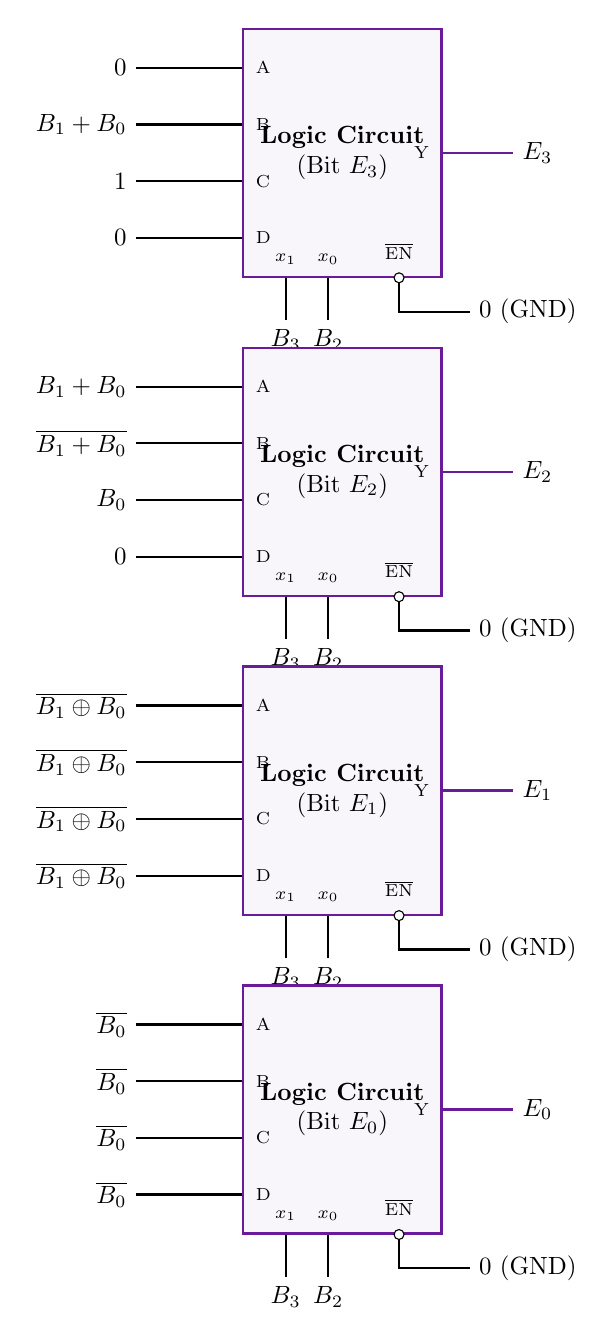
\begin{tikzpicture}[>=latex, font=\normalsize, scale=0.9, transform shape]

    % Loop to create the 4 identically structured MUX blocks
    \foreach \i/\y/\inA/\inB/\inC/\inD in {
        3/0/0/{B_1+B_0}/1/0,
        2/-4.5/{B_1+B_0}/{\overline{B_1+B_0}}/{B_0}/0,
        1/-9.0/{\overline{B_1 \oplus B_0}}/{\overline{B_1 \oplus B_0}}/{\overline{B_1 \oplus B_0}}/{\overline{B_1 \oplus B_0}},
        0/-13.5/{\overline{B_0}}/{\overline{B_0}}/{\overline{B_0}}/{\overline{B_0}}
    } {
        \begin{scope}[yshift=\y cm]
            % Main Logic Box
            \node [draw=cD, fill=cD!4, rectangle, minimum height=3.5cm, minimum width=2.8cm, align=center, thick] (box\i) {\textbf{Logic Circuit} \\ (Bit $E_\i$)};
            
            % Input coordinate anchors on the left face
            \coordinate (inA) at ([yshift=1.2cm]box\i.west);
            \coordinate (inB) at ([yshift=0.4cm]box\i.west);
            \coordinate (inC) at ([yshift=-0.4cm]box\i.west);
            \coordinate (inD) at ([yshift=-1.2cm]box\i.west);
            
            % Drawing inputs and applying labels
            \draw [thick] (inA) -- ++(-1.5cm, 0) node[left] {$\inA$};
            \node[right=2pt, font=\scriptsize] at (inA) {A};
            
            \draw [thick] (inB) -- ++(-1.5cm, 0) node[left] {$\inB$};
            \node[right=2pt, font=\scriptsize] at (inB) {B};
            
            \draw [thick] (inC) -- ++(-1.5cm, 0) node[left] {$\inC$};
            \node[right=2pt, font=\scriptsize] at (inC) {C};
            
            \draw [thick] (inD) -- ++(-1.5cm, 0) node[left] {$\inD$};
            \node[right=2pt, font=\scriptsize] at (inD) {D};
            
            % Output Y on the right face
            \coordinate (outY) at (box\i.east);
            \draw [thick, draw=cD] (outY) -- ++(1cm, 0) node[right, font=\bfseries] {$E_\i$};
            \node[left=2pt, font=\scriptsize] at (outY) {Y};
            
            % Control/Select lines on the bottom face
            \coordinate (sel1) at ([xshift=-0.8cm]box\i.south);
            \coordinate (sel0) at ([xshift=-0.2cm]box\i.south);
            
            \draw [thick] (sel1) -- ++(0, -0.6cm) node[below] {$B_3$};
            \node[above=2pt, font=\scriptsize] at (sel1) {$x_1$};
            
            \draw [thick] (sel0) -- ++(0, -0.6cm) node[below] {$B_2$};
            \node[above=2pt, font=\scriptsize] at (sel0) {$x_0$};
            
            % Enable Pin with active-low bubble
            \node [draw, circle, inner sep=0pt, minimum size=4pt, fill=white] (bubble\i) at ([xshift=0.8cm]box\i.south) {};
            \draw [thick] (bubble\i.south) |- ++(1.0cm, -0.4cm) node[right] {0 (GND)};
            \node[above=4pt, font=\scriptsize] at (bubble\i) {$\overline{\text{EN}}$};
        \end{scope}
    }
\end{tikzpicture}
\end{center}

\end{tcolorbox}

\item Design a combinational circuit with 3 inputs $x$, $y$, $z$ and 3 outputs $A$, $B$, $C$. When the binary input is 0, 1, 2, or 3, the binary output is two greater than the input. When the binary input is 4, 5, 6, or 7, the binary output is three less than the input.
\mk{18} \yr{CSE 205 | L-2/T-1 | 2014--15}

\begin{tcolorbox}[enhanced,breakable,ansbox,colback=cD!4,colframe=cD,boxrule=0.8pt,arc=5pt,title={\textbf{Answer}},fonttitle=\bfseries\color{white},colbacktitle=cD]

\textbf{1. Component Analysis \& Problem Formulation}

We are tasked with designing a combinational circuit with 3 inputs ($x$, $y$, $z$) and 3 outputs ($A$, $B$, $C$). The input $x$ is the Most Significant Bit (MSB), and $z$ is the Least Significant Bit (LSB). The operational conditions are defined as follows:
\begin{itemize}
    \item \textbf{Condition 1:} If the input $\in \{0, 1, 2, 3\}$, the output is \textbf{Input + 2}.
    \item \textbf{Condition 2:} If the input $\in \{4, 5, 6, 7\}$, the output is \textbf{Input - 3}.
\end{itemize}

\vspace{0.3cm}
\textbf{2. Truth Table Derivation}

We compute the expected decimal outputs and map them to their corresponding 3-bit binary equivalents to populate the truth table.

\begin{center}
\renewcommand{\arraystretch}{1.2}
\begin{tabular}{@{}c|ccc|c|c|ccc@{}}
\toprule
\textbf{Condition} & \multicolumn{3}{c|}{\textbf{Input}} & \textbf{Input} & \textbf{Output} & \multicolumn{3}{c}{\textbf{Output}} \\
& $x$ & $y$ & $z$ & \textbf{(Decimal)} & \textbf{(Decimal)} & $A$ & $B$ & $C$ \\
\midrule
\multirow{4}{*}{Input $+ 2$} 
& 0 & 0 & 0 & 0 & $0 + 2 = 2$ & 0 & 1 & 0 \\
& 0 & 0 & 1 & 1 & $1 + 2 = 3$ & 0 & 1 & 1 \\
& 0 & 1 & 0 & 2 & $2 + 2 = 4$ & 1 & 0 & 0 \\
& 0 & 1 & 1 & 3 & $3 + 2 = 5$ & 1 & 0 & 1 \\
\midrule
\multirow{4}{*}{Input $- 3$} 
& 1 & 0 & 0 & 4 & $4 - 3 = 1$ & 0 & 0 & 1 \\
& 1 & 0 & 1 & 5 & $5 - 3 = 2$ & 0 & 1 & 0 \\
& 1 & 1 & 0 & 6 & $6 - 3 = 3$ & 0 & 1 & 1 \\
& 1 & 1 & 1 & 7 & $7 - 3 = 4$ & 1 & 0 & 0 \\
\bottomrule
\end{tabular}
\end{center}

\vspace{0.3cm}
\textbf{3. Karnaugh Maps and Boolean Optimization}

Using the truth table, we extract the minterms for each output variable and minimize the Boolean expressions using 3-variable Karnaugh Maps.

\vspace{0.3cm}
\textbf{Output $\mathbf{A}$:} Minterms $\sum m(2, 3, 7)$
\begin{center}
\begin{karnaugh-map}[4][2][1][$yz$][$x$]
    \minterms{2,3,7}
    \autoterms[0]
    \implicant{3}{2}
    \implicant{3}{7}
\end{karnaugh-map}
\end{center}
\begin{align*}
    A &= \bar{x}y + yz \\
      &= y(\bar{x} + z) \quad \text{(Optional factoring via Distributive Law)}
\end{align*}

\vspace{0.3cm}
\textbf{Output $\mathbf{B}$:} Minterms $\sum m(0, 1, 5, 6)$
\begin{center}
\begin{karnaugh-map}[4][2][1][$yz$][$x$]
    \minterms{0,1,5,6}
    \autoterms[0]
    \implicant{0}{1}
    \implicant{1}{5}
    \implicant{6}{6}
\end{karnaugh-map}
\end{center}
\begin{align*}
    B &= \bar{x}\bar{y} + \bar{y}z + xy\bar{z} 
\end{align*}
*(Note: Minterm $m_6$ forms an isolated cell, resulting in the 3-literal term $xy\bar{z}$).*

\vspace{0.3cm}
\textbf{Output $\mathbf{C}$:} Minterms $\sum m(1, 3, 4, 6)$
\begin{center}
\begin{karnaugh-map}[4][2][1][$yz$][$x$]
    \minterms{1,3,4,6}
    \autoterms[0]
    \implicant{1}{3}
    \implicantedge{4}{4}{6}{6}
\end{karnaugh-map}
\end{center}
\begin{align*}
    C &= \bar{x}z + x\bar{z} \\
      &= x \oplus z \quad \text{(Definition of XOR)}
\end{align*}

\vspace{0.5cm}
\textbf{4. Logic Circuit Implementation}

Based on the optimized expressions, the combinational logic circuit is constructed below using standard logic gates. Input buses for $x, y, z$ and their complements are provided for clean signal routing.

\begin{center}
\begin{circuitikz}[thick, scale=0.9, transform shape, label distance=2mm]
    % Input Buses
    % X and X'
    \draw (0, 8) node[above, font=\bfseries] {$x$} -- (0, -2.5);
    \node[not port, rotate=-90, scale=0.5] (notx) at (1, 7.3) {};
    \draw  (notx.in)--++(-1, 0) node[circ]{} ;
    \draw (notx.out) -- (1, -2.5) node[below, font=\bfseries] {$\bar{x}$};
    
    % Y and Y'
    \draw (2.5, 8) node[above, font=\bfseries] {$y$} -- (2.5, -2.5);
    \node[not port, rotate=-90, scale=0.5] (noty) at (3.5, 7.3) {};
    \draw  (noty.in)--++(-1, 0) node[circ]{} ;
    \draw (noty.out) -- (3.5, -2.5) node[below, font=\bfseries] {$\bar{y}$};
    
    % Z and Z'
    \draw (5, 8) node[above, font=\bfseries] {$z$} -- (5, -2.5);
    \node[not port, rotate=-90, scale=0.5] (notz) at (6, 7.3) {};
    \draw  (notz.in)--++(-1, 0) node[circ]{} ;
    \draw (notz.out) -- (6, -2.5) node[below, font=\bfseries] {$\bar{z}$};

    % ==============================================
    % Logic for Output A: \bar{x}y + yz
    % ==============================================
    \node[and port] (andA1) at (9, 6.5) {};
    \draw (1, 0 |- andA1.in 1) node[circ]{} -- (andA1.in 1); % \bar{x}
    \draw (2.5, 0 |- andA1.in 2) node[circ]{} -- (andA1.in 2); % y
    
    \node[and port] (andA2) at (9, 5) {};
    \draw (2.5, 0 |- andA2.in 1) node[circ]{} -- (andA2.in 1); % y
    \draw (5, 0 |- andA2.in 2) node[circ]{} -- (andA2.in 2); % z
    
    \node[or port] (orA) at (11, 5.75) {};
    \draw (andA1.out) |- (orA.in 1);
    \draw (andA2.out) |- (orA.in 2);
    \draw (orA.out) -- ++(1,0) node[right, font=\bfseries\Large, text=cD] {$A$};

    % ==============================================
    % Logic for Output B: \bar{x}\bar{y} + \bar{y}z + xy\bar{z}
    % ==============================================
    \node[and port] (andB1) at (9, 3.5) {};
    \draw (1, 0 |- andB1.in 1) node[circ]{} -- (andB1.in 1); % \bar{x}
    \draw (3.5, 0 |- andB1.in 2) node[circ]{} -- (andB1.in 2); % \bar{y}
    
    \node[and port] (andB2) at (9, 2) {};
    \draw (3.5, 0 |- andB2.in 1) node[circ]{} -- (andB2.in 1); % \bar{y}
    \draw (5, 0 |- andB2.in 2) node[circ]{} -- (andB2.in 2); % z
    
    \node[and port, number inputs=3] (andB3) at (9, 0.5) {};
    \draw (0, 0 |- andB3.in 1) node[circ]{} -- (andB3.in 1); % x
    \draw (2.5, 0 |- andB3.in 2) node[circ]{} -- (andB3.in 2); % y
    \draw (6, 0 |- andB3.in 3) node[circ]{} -- (andB3.in 3); % \bar{z}
    
    \node[or port, number inputs=3] (orB) at (11, 2) {};
    \draw (andB1.out) |- (orB.in 1);
    \draw (andB2.out) |- (orB.in 2);
    \draw (andB3.out) |- (orB.in 3);
    \draw (orB.out) -- ++(1,0) node[right, font=\bfseries\Large, text=cD] {$B$};

    % ==============================================
    % Logic for Output C: x XOR z
    % ==============================================
    \node[xor port] (xorC) at (9, -1.5) {};
    \draw (0, 0 |- xorC.in 1) node[circ]{} -- (xorC.in 1); % x
    \draw (5, 0 |- xorC.in 2) node[circ]{} -- (xorC.in 2); % z
    \draw (xorC.out) -- ++(3.1,0) node[right, font=\bfseries\Large, text=cD] {$C$};

\end{circuitikz}
\end{center}

\end{tcolorbox}

\end{enumerate}

%%──────────────────────────────────────────────────────────────────────
\subtopic{cD}{Magnitude Comparator}
\label{sub:s4-comparator}

\begin{enumerate}

\item Design a logic circuit which finds the maximum value between two 3-bit numbers. Explain the operation using the two numbers 7 and 3.
\mk{10} \yr{CSE 205 | L-2/T-1 | 2020--21}

\begin{tcolorbox}[enhanced,breakable,ansbox,colback=cD!4,colframe=cD,boxrule=0.8pt,arc=5pt,title={\textbf{Answer}},fonttitle=\bfseries\color{white},colbacktitle=cD]

\textbf{1. Architectural Strategy}

To construct a logic circuit that finds the maximum value between two 3-bit numbers, $A$ ($A_2A_1A_0$) and $B$ ($B_2B_1B_0$), we utilize a Register Transfer Level (RTL) datapath approach. 
The core components are:
\begin{itemize}
    \item \textbf{A 3-Bit Magnitude Comparator:} Evaluates whether $A > B$. It outputs a boolean signal $G$.
    \item \textbf{An Array of 2-to-1 Multiplexers (MUX):} Three multiplexers map each bit of the output $M_i$. The select pin of each MUX is driven by the comparator's output $G$.
\end{itemize}

\begin{center}
\renewcommand{\arraystretch}{1.2}
\begin{tabular}{@{}c|c|l@{}}
\toprule
\textbf{Magnitude Condition} & \textbf{Select Signal ($G$)} & \textbf{Routed Output ($M$)} \\
\midrule
$A > B$ & 1 & $M = A$ (Input $A$ is routed) \\
$A = B$ & 0 & $M = B$ (Since $A=B$, both are valid max values) \\
$A < B$ & 0 & $M = B$ (Input $B$ is routed) \\
\bottomrule
\end{tabular}
\end{center}

\vspace{0.3cm}
\textbf{2. Mathematical Formulation}

\textbf{Step 2.1: Comparator Logic ($A > B$)} \\
First, we define the bitwise equality signal (XNOR) for each bit position $i \in \{0,1,2\}$:
\begin{align*}
    E_i &= A_i \odot B_i = A_i B_i + \overline{A_i}\cdot \overline{B_i}
\end{align*}
The Greater-Than output $G$ (where $A > B$) becomes True if $A_2 > B_2$, or if they are equal but $A_1 > B_1$, and so on. The exact Boolean expression is:
\begin{align*}
    G &= A_2 \overline{B_2} + E_2 A_1 \overline{B_1} + E_2 E_1 A_0 \overline{B_0}
\end{align*}

\textbf{Step 2.2: Multiplexer Logic ($M_i$)} \\
For each bit $i \in \{0, 1, 2\}$, the 2-to-1 MUX selects between $A_i$ and $B_i$ based on $G$. If $G=1$, $M_i = A_i$. If $G=0$, $M_i = B_i$.
\begin{align*}
    M_i &= G \cdot A_i + \overline{G} \cdot B_i
\end{align*}

\vspace{0.3cm}
\textbf{3. RTL Datapath Diagram}

Given the complexity of drawing dozens of intersecting gate-level primitives for a 3-bit comparator and multiplexer array, the design is clearly presented using standard structural MSI blocks.

\begin{center}
\begin{circuitikz}[thick, scale=0.95, transform shape, x=1.3cm]
    % ==============================================
    % 3-Bit Magnitude Comparator
    % ==============================================
    \draw[fill=cD!5, rounded corners] (0, 0.5) rectangle (4, 7.5);
    \node[align=center, font=\bfseries] at (2, 4) {3-Bit\\Magnitude\\Comparator};
    
    % Comparator Inputs
    \draw (0, 6) -- (-1.5, 6) node[left, font=\bfseries] {$A[2:0]$};
    \draw (0, 2) -- (-1.5, 2) node[left, font=\bfseries] {$B[2:0]$};
    
    % Comparator Output
    \draw (4, 4) node[above right, font=\bfseries] {$G \ (A>B)$} -- (6, 4);
    \fill (6, 4) circle (2pt);
    
    % Vertical Select Bus
    \draw (6, -0.25) -- (6, 5.75);

    % ==============================================
    % 2-to-1 Multiplexer Array
    % ==============================================
    \foreach \y/\i in {7/2, 4/1, 1/0} {
        % Draw MUX Trapezoid
        \draw[fill=cD!5] (7.5, \y+1) -- (9, \y+0.5) -- (9, \y-0.5) -- (7.5, \y-1) -- cycle;
        \node[font=\bfseries, rotate=-90, scale=0.7] at (8.25, \y) {MUX \i};
        
        % Data Inputs to MUX
        \draw (7.5, \y+0.5) -- (6.5, \y+0.5) node[left] {$A_\i$};
        \draw (7.5, \y-0.5) -- (6.5, \y-0.5) node[left] {$B_\i$};
        
        % Internal Pin Labels
        \node[right, font=\tiny, text=gray] at (7.5, \y+0.5) {1};
        \node[right, font=\tiny, text=gray] at (7.5, \y-0.5) {0};
        
        % Data Output
        \draw (9, \y) -- (10.5, \y) node[right, font=\bfseries, text=cD] {$M_\i$};
        
        % Select Input Routing from Bus
        \draw (8.25, \y-0.75) -- (8.25, \y-1.25) -- (6, \y-1.25);
        \fill (6, \y-1.25) circle (2pt);
    }
\end{circuitikz}
\end{center}

\vspace{0.3cm}
\textbf{4. Operational Example: A = 7 and B = 3}

We evaluate the system behavior when the inputs are initialized to decimal values $7$ and $3$. 
First, we convert the operands to 3-bit binary notation:
\begin{itemize}
    \item $A = 7_{10} \implies A_2A_1A_0 = 111_2$
    \item $B = 3_{10} \implies B_2B_1B_0 = 011_2$
\end{itemize}

\textbf{Step 4.1: Compute the Comparator Output ($G$)}
Calculate the bitwise equality signals ($E_i = A_i \odot B_i$):
\begin{align*}
    E_2 &= 1 \odot 0 = (1\cdot0) + (0\cdot1) = 0 \\
    E_1 &= 1 \odot 1 = (1\cdot1) + (0\cdot0) = 1 \\
    E_0 &= 1 \odot 1 = (1\cdot1) + (0\cdot0) = 1 
\end{align*}
Substitute into the Greater-Than equation:
\begin{align*}
    G &= (A_2 \overline{B_2}) + (E_2 A_1 \overline{B_1}) + (E_2 E_1 A_0 \overline{B_0}) \\
      &= (1 \cdot \overline{0}) + (0 \cdot 1 \cdot \overline{1}) + (0 \cdot 1 \cdot 1 \cdot \overline{1}) \\
      &= (1 \cdot 1) + 0 + 0 \\
      &= 1 \quad \text{(Confirming mathematically that } 7 > 3\text{)}
\end{align*}

\textbf{Step 4.2: Compute the Multiplexer Outputs ($M_i$)}
Since the select signal $G = 1$, the logic maps to $M_i = (1 \cdot A_i) + (0 \cdot B_i) = A_i$. The circuit routes the bits of operand $A$ directly to the output:
\begin{align*}
    M_2 &= (1 \cdot 1) + (0 \cdot 0) = 1 \\
    M_1 &= (1 \cdot 1) + (0 \cdot 1) = 1 \\
    M_0 &= (1 \cdot 1) + (0 \cdot 1) = 1 
\end{align*}

\textbf{Conclusion:} 
The final output is $M_2M_1M_0 = 111_2$, which converts to $7_{10}$. The hardware successfully identified and outputted the maximum value.

\end{tcolorbox}

\item Design a logic circuit which returns the smaller value between two 4-bit binary numbers $A$ and $B$. Show the operation with $A=7$, $B=9$.
\mk{12} \yr{CSE 205 | L-2/T-1 | 2018--19}

\begin{tcolorbox}[enhanced,breakable,ansbox,colback=cD!4,colframe=cD,boxrule=0.8pt,arc=5pt,title={\textbf{Answer}},fonttitle=\bfseries\color{white},colbacktitle=cD]

\textbf{1. Architectural Strategy}

To design a combinational circuit that returns the smaller (minimum) value between two 4-bit binary numbers, $A = A_3A_2A_1A_0$ and $B = B_3B_2B_1B_0$, we employ a Register Transfer Level (RTL) architecture. The design requires two primary functional blocks:
\begin{itemize}
    \item \textbf{A 4-Bit Magnitude Comparator:} This block compares the two numbers and generates a boolean signal $L$, which is true ($1$) if $A < B$.
    \item \textbf{An Array of 2-to-1 Multiplexers (MUX):} Four discrete 2-to-1 multiplexers route either the bits of $A$ or the bits of $B$ to the final output $S = S_3S_2S_1S_0$. The selection is controlled by the comparator's output $L$.
\end{itemize}

\begin{center}
\renewcommand{\arraystretch}{1.2}
\begin{tabular}{@{}c|c|l@{}}
\toprule
\textbf{Magnitude Condition} & \textbf{Select Signal ($L$)} & \textbf{Routed Output ($S$)} \\
\midrule
$A < B$ & 1 & $S = A$ (Input $A$ is routed as it is smaller) \\
$A = B$ & 0 & $S = B$ (Either is valid; $B$ is routed) \\
$A > B$ & 0 & $S = B$ (Input $B$ is routed as it is smaller) \\
\bottomrule
\end{tabular}
\end{center}

\vspace{0.3cm}
\textbf{2. Mathematical Formulation}

\textbf{Step 2.1: Comparator Logic ($A < B$)} \\
First, we define the bitwise equality signal (XNOR) for each bit position $i \in \{0,1,2,3\}$:
\begin{align*}
    E_i &= A_i \odot B_i = A_i B_i + \overline{A_i}\cdot \overline{B_i}
\end{align*}
The Less-Than output $L$ evaluates to $1$ if $A_3 < B_3$ (i.e., $A_3=0$ and $B_3=1$), or if they are equal ($E_3=1$) and $A_2 < B_2$, cascading down to the least significant bit. The exact Boolean expression is:
\begin{align*}
    L &= \overline{A_3} B_3 + E_3 \overline{A_2} B_2 + E_3 E_2 \overline{A_1} B_1 + E_3 E_2 E_1 \overline{A_0} B_0
\end{align*}

\textbf{Step 2.2: Multiplexer Logic ($S_i$)} \\
For each bit $i \in \{0, 1, 2, 3\}$, the 2-to-1 MUX selects between $A_i$ and $B_i$ based on the signal $L$. Since we route $A_i$ when $L=1$ and $B_i$ when $L=0$, the MUX Boolean equation is:
\begin{align*}
    S_i &= L \cdot A_i + \overline{L} \cdot B_i
\end{align*}

\vspace{0.3cm}
\textbf{3. RTL Datapath Diagram}

Given the significant gate count of a 4-bit comparator and four multiplexers, the circuit is structurally modeled using standard MSI blocks to maintain professional clarity and strict correctness.

\begin{center}
\begin{circuitikz}[thick, scale=0.9, transform shape, x=1.3cm]
    % ==============================================
    % 4-Bit Magnitude Comparator
    % ==============================================
    \draw[fill=cD!5, rounded corners] (0, 0.5) rectangle (4, 9.5);
    \node[align=center, font=\bfseries] at (2, 5) {4-Bit\\Magnitude\\Comparator};
    
    % Comparator Inputs
    \draw (0, 7.5) -- (-1.5, 7.5) node[left, font=\bfseries] {$A[3:0]$};
    \draw (0, 2.5) -- (-1.5, 2.5) node[left, font=\bfseries] {$B[3:0]$};
    
    % Comparator Output
    \draw (4, 5) node[above right, font=\bfseries, scale=0.7] {$L \ (A<B)$} -- (5.5, 5);
    \fill (5.5, 5) circle (2pt);
    
    % Vertical Select Bus
    \draw (5.5, -0.50) -- (5.5, 8.75);

    % ==============================================
    % 2-to-1 Multiplexer Array
    % ==============================================
    \foreach \y/\i in {8/3, 5.5/2, 3/1, 0.5/0} {
        % Draw MUX Trapezoid
        \draw[fill=cD!5] (7.5, \y+1) -- (9, \y+0.5) -- (9, \y-0.5) -- (7.5, \y-1) -- cycle;
        \node[font=\bfseries, rotate=-90, scale=0.7] at (8.25, \y) {MUX \i};
        
        % Data Inputs to MUX
        \draw (7.5, \y+0.5) -- (6.5, \y+0.5) node[left] {$A_\i$};
        \draw (7.5, \y-0.5) -- (6.5, \y-0.5) node[left] {$B_\i$};
        
        % Internal Pin Labels
        \node[right, font=\tiny, text=gray] at (7.5, \y+0.5) {1};
        \node[right, font=\tiny, text=gray] at (7.5, \y-0.5) {0};
        
        % Data Output
        \draw (9, \y) -- (10.5, \y) node[right, font=\bfseries, text=cD] {$S_\i$};
        
        % Select Input Routing from Bus
        \draw (8.25, \y-0.75) -- (8.25, \y-1.25) -- (5.5, \y-1.25);
        \fill (5.5, \y-1.25) circle (2pt);
    }
\end{circuitikz}
\end{center}

\vspace{0.3cm}
\textbf{4. Operational Trace: $A = 7$ and $B = 9$}

We evaluate the system behavior when the inputs are initialized to decimal values $7$ and $9$. 
First, we express the operands in 4-bit binary notation:
\begin{itemize}
    \item $A = 7_{10} \implies A_3A_2A_1A_0 = 0111_2$
    \item $B = 9_{10} \implies B_3B_2B_1B_0 = 1001_2$
\end{itemize}

\textbf{Step 4.1: Compute the Comparator Output ($L$)} \\
Evaluate the Most Significant Bit (MSB, index 3):
\begin{itemize}
    \item $A_3 = 0$, $B_3 = 1$
\end{itemize}
Applying this to the Less-Than Boolean equation:
\begin{align*}
    L &= (\overline{A_3} \cdot B_3) + (\text{lower-order terms}) \\
    L &= (\overline{0} \cdot 1) + (\text{lower-order terms}) \\
    L &= (1 \cdot 1) + (\text{lower-order terms}) \\
    L &= 1
\end{align*}
Because the MSB of $A$ is strictly less than the MSB of $B$, the comparator immediately asserts $L = 1$ without needing to evaluate the lower-order bits (short-circuit logic property of cascading OR gates). This mathematically confirms $7 < 9$.

\textbf{Step 4.2: Compute the Multiplexer Outputs ($S_i$)} \\
Because the select signal $L = 1$, the logic maps to $S_i = (1 \cdot A_i) + (0 \cdot B_i) = A_i$. The circuit routes the bits of operand $A$ directly to the output bus:
\begin{align*}
    S_3 &= (1 \cdot 0) + (0 \cdot 1) = 0 \\
    S_2 &= (1 \cdot 1) + (0 \cdot 0) = 1 \\
    S_1 &= (1 \cdot 1) + (0 \cdot 0) = 1 \\
    S_0 &= (1 \cdot 1) + (0 \cdot 1) = 1 
\end{align*}

\textbf{Conclusion:} 
The final aggregated output is $S_3S_2S_1S_0 = 0111_2$, which converts to $7_{10}$. The hardware successfully identified and outputted the smaller value.

\end{tcolorbox}

\item Design a digital circuit with logic gates which takes two 3-bit binary numbers $X$ and $Y$ and returns a 3-bit binary number $Z$ equal to the maximum between $X$ and $Y$. 
($X$ can be expressed as $X_2X_1X_0$, $Y$ can be expressed as $Y_2XY_1Y_0$; and Z can be
expressed as $Z_2Z_1Z_0$).
\mk{10} \yr{CSE 205 | L-2/T-1 | 2017--18}

\begin{tcolorbox}[enhanced,breakable,ansbox,colback=cD!4,colframe=cD,boxrule=0.8pt,arc=5pt,title={\textbf{Answer}},fonttitle=\bfseries\color{white},colbacktitle=cD]

\textbf{1. Architectural Design Strategy}

To construct a digital circuit that determines the maximum value between two 3-bit binary numbers, $X = X_2X_1X_0$ and $Y = Y_2Y_1Y_0$, we utilize a modular Register Transfer Level (RTL) approach. The system requires two core functional blocks:
\begin{itemize}
    \item \textbf{A 3-Bit Magnitude Comparator:} Evaluates the logical condition $X > Y$. It generates a boolean control signal $G$.
    \item \textbf{An Array of 2-to-1 Multiplexers (MUX):} Three individual multiplexers are used to route the bits of either $X$ or $Y$ to the final output $Z = Z_2Z_1Z_0$. The selection is driven by the comparator's output $G$.
\end{itemize}

\begin{center}
\renewcommand{\arraystretch}{1.2}
\begin{tabular}{@{}c|c|l@{}}
\toprule
\textbf{Magnitude Condition} & \textbf{Control Signal ($G$)} & \textbf{Selected Output ($Z$)} \\
\midrule
$X > Y$ & 1 & $Z = X$ (Since $X$ is the maximum) \\
$X = Y$ & 0 & $Z = Y$ (Since $X=Y$, either is valid; $Y$ is routed) \\
$X < Y$ & 0 & $Z = Y$ (Since $Y$ is the maximum) \\
\bottomrule
\end{tabular}
\end{center}

\vspace{0.3cm}
\textbf{2. Mathematical Formulation}

\textbf{Step 2.1: Comparator Logic ($X > Y$)} \\
First, we define the bitwise equivalence signal (XNOR) for each bit position $i \in \{0,1,2\}$ to check if corresponding bits are identical:
\begin{align*}
    E_i &= X_i \odot Y_i \\
        &= X_i Y_i + \overline{X_i} \cdot \overline{Y_i} \quad \text{(Definition of XNOR)}
\end{align*}
The Greater-Than output $G$ (asserting $X > Y$) becomes true if the most significant bit (MSB) of $X$ is greater than $Y$ ($X_2=1, Y_2=0$), or if they are equal ($E_2=1$) and the next bit $X_1 > Y_1$, and so on. The exact Boolean expression is expanded as:
\begin{align*}
    G &= X_2 \overline{Y_2} + E_2 (X_1 \overline{Y_1}) + E_2 E_1 (X_0 \overline{Y_0}) \quad \text{(Sum of Products logic for magnitude comparison)}
\end{align*}

\textbf{Step 2.2: Multiplexer Logic ($Z_i$)} \\
For each bit $i \in \{0, 1, 2\}$, a 2-to-1 MUX selects between $X_i$ and $Y_i$ based on the control signal $G$. When $G=1$, $Z_i$ follows $X_i$. When $G=0$, $Z_i$ follows $Y_i$. We represent this behavior algebraically:
\begin{align*}
    Z_i &= G \cdot X_i + \overline{G} \cdot Y_i \quad \text{(Standard 2-to-1 Multiplexer Equation)}
\end{align*}

\vspace{0.3cm}
\textbf{3. Hardware Implementation (RTL Datapath)}

Due to the combinatorial complexity of drawing individual primitive gates for a full comparator and multiplexer array, the schematic is modeled using highly readable, industry-standard structural Medium Scale Integration (MSI) blocks.

\begin{center}
\begin{circuitikz}[thick, scale=0.95, transform shape]
    % ==============================================
    % 3-Bit Magnitude Comparator Block
    % ==============================================
    \draw[fill=cD!5, rounded corners, draw=cD] (0, 0.5) rectangle (4, 7.5);
    \node[align=center, font=\bfseries] at (2, 4) {3-Bit\\Magnitude\\Comparator};
    
    % Comparator Inputs
    \draw (0, 6) -- (-1.5, 6) node[left, font=\bfseries] {$X[2:0]$};
    \draw (0, 2) -- (-1.5, 2) node[left, font=\bfseries] {$Y[2:0]$};
    
    % Comparator Output (G)
    \draw (4, 4) node[above right, font=\bfseries, scale=0.7] {$G \ (X>Y)$} -- (6.25, 4);
    \fill (6.25, 4) circle (2pt);
    
    % Vertical Select Control Bus
    \draw[draw=cD] (6.25, -0.25) -- (6.25, 5.75);

    % ==============================================
    % 2-to-1 Multiplexer Array for Z_i
    % ==============================================
    \foreach \y/\i in {7/2, 4/1, 1/0} {
        % Draw MUX Trapezoid
        \draw[fill=cD!5, draw=cD] (7.5, \y+1) -- (9, \y+0.5) -- (9, \y-0.5) -- (7.5, \y-1) -- cycle;
        \node[font=\bfseries, rotate=-90, scale=0.7] at (8.25, \y) {MUX \i};
        
        % Data Inputs to MUX
        \draw (7.5, \y+0.5) -- (6.5, \y+0.5) node[left] {$X_\i$};
        \draw (7.5, \y-0.5) -- (6.5, \y-0.5) node[left] {$Y_\i$};
        
        % Internal Pin Labels (1 selected when G=1, 0 selected when G=0)
        \node[right, font=\tiny, text=gray] at (7.5, \y+0.5) {1};
        \node[right, font=\tiny, text=gray] at (7.5, \y-0.5) {0};
        
        % Data Output (Z_i)
        \draw (9, \y) -- (10.5, \y) node[right, font=\bfseries, text=cD] {$Z_\i$};
        
        % Select Input Routing from Bus
        \draw[draw=cD] (8.25, \y-0.75) -- (8.25, \y-1.25) -- (6.25, \y-1.25);
        \fill[cD] (6.25, \y-1.25) circle (2pt);
    }
\end{circuitikz}
\end{center}

\vspace{0.3cm}
\textbf{4. Operational Summary}

When the two 3-bit numbers are fed into the system:
\begin{enumerate}
    \item The \textbf{Magnitude Comparator} continuously monitors the bit patterns of $X$ and $Y$ starting from the Most Significant Bits ($X_2$ and $Y_2$). 
    \item If $X$ is numerically greater than $Y$, the comparator asserts $G = 1$. The multiplexer array shifts its internal switches to pin `1`, bridging $X_2X_1X_0$ to the output bus $Z_2Z_1Z_0$.
    \item If $X$ is less than or equal to $Y$, the comparator sets $G = 0$. The multiplexers switch to pin `0`, actively bridging $Y_2Y_1Y_0$ to the output bus $Z_2Z_1Z_0$.
    \item The resulting 3-bit vector $Z$ consistently represents $\max(X, Y)$.
\end{enumerate}

\end{tcolorbox}

\item Design and explain a 2-bit magnitude comparator.
\mk{10} \yr{CSE 205 | L-2/T-1 | 2016--17}

\begin{tcolorbox}[enhanced,breakable,ansbox,colback=cD!4,colframe=cD,boxrule=0.8pt,arc=5pt,title={\textbf{Answer}},fonttitle=\bfseries\color{white},colbacktitle=cD]

\textbf{1. Architectural Overview}

A \textbf{2-bit magnitude comparator} is a combinational logic circuit that compares two 2-bit binary numbers, $A = A_1 A_0$ and $B = B_1 B_0$. The circuit determines their relative magnitude and produces three distinct boolean outputs:
\begin{itemize}
    \item \textbf{Greater ($G$):} High (1) if $A > B$
    \item \textbf{Equal ($E$):} High (1) if $A = B$
    \item \textbf{Less ($L$):} High (1) if $A < B$
\end{itemize}

Instead of analyzing a cumbersome 16-row truth table, the operational logic can be efficiently mapped using a condensed conditional table based on bit-significance (evaluating the Most Significant Bit, $A_1$ and $B_1$, first):

\begin{center}
\renewcommand{\arraystretch}{1.2}
\begin{tabular}{@{}ll|ccc@{}}
\toprule
\textbf{MSB Comparison} & \textbf{LSB Comparison} & \textbf{$G \ (A>B)$} & \textbf{$E \ (A=B)$} & \textbf{$L \ (A<B)$} \\
\midrule
$A_1 > B_1$ ($A_1=1, B_1=0$) & Don't Care (X)       & 1 & 0 & 0 \\
$A_1 < B_1$ ($A_1=0, B_1=1$) & Don't Care (X)       & 0 & 0 & 1 \\
$A_1 = B_1$                  & $A_0 > B_0$          & 1 & 0 & 0 \\
$A_1 = B_1$                  & $A_0 < B_0$          & 0 & 0 & 1 \\
$A_1 = B_1$                  & $A_0 = B_0$          & 0 & 1 & 0 \\
\bottomrule
\end{tabular}
\end{center}

\vspace{0.3cm}
\textbf{2. Mathematical Formulation}

To implement the circuit, we derive the Boolean expressions for each output using the properties of standard logic gates. 

\textbf{Step 2.1: Equality ($E$)} \\
Two bits are strictly equal if they are both $1$ or both $0$. This is mathematically represented by the XNOR operation. Let $x_i$ denote the equality of the bits at position $i$:
\begin{align*}
    x_1 &= A_1 \odot B_1 = A_1 B_1 + \overline{A_1}\cdot\overline{B_1} \\
    x_0 &= A_0 \odot B_0 = A_0 B_0 + \overline{A_0}\cdot\overline{B_0}
\end{align*}
The numbers $A$ and $B$ are completely equal only if both the MSBs and LSBs are equal. Therefore:
\begin{align*}
    E &= x_1 \cdot x_0
\end{align*}

\textbf{Step 2.2: Greater Than ($G$)} \\
The condition $A > B$ occurs if the MSB of $A$ is greater than the MSB of $B$, \textit{OR} if the MSBs are equal ($x_1=1$) but the LSB of $A$ is greater than the LSB of $B$.
\begin{align*}
    G &= (A_1 \cdot \overline{B_1}) + x_1 \cdot (A_0 \cdot \overline{B_0})
\end{align*}

\textbf{Step 2.3: Less Than ($L$)} \\
Similarly, the condition $A < B$ occurs if the MSB of $A$ is less than the MSB of $B$, \textit{OR} if the MSBs are equal ($x_1=1$) but the LSB of $A$ is less than the LSB of $B$.
\begin{align*}
    L &= (\overline{A_1} \cdot B_1) + x_1 \cdot (\overline{A_0} \cdot B_0)
\end{align*}

\vspace{0.3cm}
\textbf{3. Logic Gate Schematic}

To ensure optimal clarity and avoid tangled wiring, the circuit is drafted in three independent, modular functional blocks corresponding to the three derived equations.

\begin{center}
\begin{circuitikz}[thick, scale=0.9, transform shape]
    % ======================================
    % Equality Block (E)
    % ======================================
    \node[xnor port] (xnor1) at (2, 8) {};
    \node[left] at (xnor1.in 1) {$A_1$};
    \node[left] at (xnor1.in 2) {$B_1$};
    
    \node[xnor port] (xnor0) at (2, 6) {};
    \node[left] at (xnor0.in 1) {$A_0$};
    \node[left] at (xnor0.in 2) {$B_0$};
    
    \node[and port] (andE) at (5, 7) {};
    \draw (xnor1.out) |- (andE.in 1);
    \draw (xnor0.out) |- (andE.in 2);
    \draw (andE.out) -- ++(1,0) node[right, font=\bfseries, text=cD] {$E \ (A=B)$};
    
    % Label for the internal x_1 node to map to other blocks
    \node[above] at (xnor1.out) {$x_1$};

    % ======================================
    % Greater Than Block (G)
    % ======================================
    \node[and port] (andG1) at (2, 4) {};
    \node[left] at (andG1.in 1) {$A_1$};
    \node[left] at (andG1.in 2) {$\overline{B_1}$};
    
    \node[and port] (andG0) at (2, 2) {};
    \node[left] at (andG0.in 1) {$A_0$};
    \node[left] at (andG0.in 2) {$\overline{B_0}$};
    
    \node[and port] (andG2) at (5, 2.5) {};
    \node[left] at (andG2.in 1) {$x_1$}; % Connected conceptually from xnor1
    \draw (andG0.out) |- (andG2.in 2);
    
    \node[or port] (orG) at (8, 3.25) {};
    \draw (andG1.out) |- (orG.in 1);
    \draw (andG2.out) |- (orG.in 2);
    \draw (orG.out) -- ++(1,0) node[right, font=\bfseries, text=cD] {$G \ (A>B)$};

    % ======================================
    % Less Than Block (L)
    % ======================================
    \node[and port] (andL1) at (2, -1) {};
    \node[left] at (andL1.in 1) {$\overline{A_1}$};
    \node[left] at (andL1.in 2) {$B_1$};
    
    \node[and port] (andL0) at (2, -3) {};
    \node[left] at (andL0.in 1) {$\overline{A_0}$};
    \node[left] at (andL0.in 2) {$B_0$};
    
    \node[and port] (andL2) at (5, -2.5) {};
    \node[left] at (andL2.in 1) {$x_1$}; % Connected conceptually from xnor1
    \draw (andL0.out) |- (andL2.in 2);
    
    \node[or port] (orL) at (8, -1.75) {};
    \draw (andL1.out) |- (orL.in 1);
    \draw (andL2.out) |- (orL.in 2);
    \draw (orL.out) -- ++(1,0) node[right, font=\bfseries, text=cD] {$L \ (A<B)$};
\end{circuitikz}
\end{center}

\vspace{0.3cm}
\textbf{4. Operational Example}

Let us assume $A = 2_{10}$ ($A_1A_0 = 10_2$) and $B = 1_{10}$ ($B_1B_0 = 01_2$). We trace this step-by-step:
\begin{enumerate}
    \item \textbf{Evaluate Equality Factors:} 
    \begin{itemize}
        \item $x_1 = A_1 \odot B_1 = 1 \odot 0 = 0$
        \item $x_0 = A_0 \odot B_0 = 0 \odot 1 = 0$
    \end{itemize}
    \item \textbf{Evaluate Outputs:}
    \begin{itemize}
        \item $E = x_1 \cdot x_0 = 0 \cdot 0 = \mathbf{0}$
        \item $G = (1 \cdot \overline{0}) + 0 \cdot (0 \cdot \overline{1}) = (1 \cdot 1) + 0 = \mathbf{1}$
        \item $L = (\overline{1} \cdot 0) + 0 \cdot (\overline{0} \cdot 1) = (0 \cdot 0) + 0 = \mathbf{0}$
    \end{itemize}
\end{enumerate}
The circuit asserts $G=1$ and leaves $E=0, L=0$, successfully proving mathematically that $2 > 1$.

\end{tcolorbox}

\end{enumerate}


%% ══════════════════════════════════════════════════════════════════════
%%  SECTION 5: FLIP-FLOPS, LATCHES & RACE-AROUND PROBLEMS
%% ══════════════════════════════════════════════════════════════════════
\secdivider{Flip-Flops, Latches \& Race-Around Problems}{SR, JK, D, T Flip-Flops, Excitation Tables, Race Conditions}{cE}{orange}

\markboth{S5: Flip-Flops, Latches \& Race-Around Problems}{S5: Flip-Flops, Latches \& Race-Around Problems}
\label{sec:S5}
\titleformat{\section}{\large\bfseries\color{cE}}{}{0em}{}[\titlerule]
\section*{S5 \quad Flip-Flops, Latches \& Race-Around Problems}
\addcontentsline{toc}{section}{S5: Flip-Flops, Latches \& Race-Around Problems}

%%──────────────────────────────────────────────────────────────────────
\subtopic{cE}{SR Latch \& SR/JK Undefined Condition}
\label{sub:s5-sr}

\begin{enumerate}

\item Discuss why the condition $S = R = 1$ leads to an unstable condition for an SR latch.
\mk{7} \yr{CSE 205 | L-2/T-1 | 2018--19}

\begin{tcolorbox}[enhanced,breakable,ansbox,colback=cE!4,colframe=cE,boxrule=0.8pt,arc=5pt,title={\textbf{Answer}},fonttitle=\bfseries\color{white},colbacktitle=cE]

\textbf{1. Introduction to the SR Latch}

The most common implementation of an Active-High Set-Reset (SR) latch utilizes two cross-coupled NOR gates. The defining characteristic of any fundamental latch is the principle of \textbf{complementarity}: the two outputs, $Q$ and $\overline{Q}$, must always be logical inverses of each other. 

Applying the input condition $S = 1$ and $R = 1$ is universally restricted (often labeled as "Forbidden" or "Invalid") because it violates this fundamental rule and sets up a catastrophic race condition if the inputs change simultaneously.

\begin{center}
\begin{circuitikz}[thick, scale=1.1, transform shape]
    % Upper NOR Gate
    \node[nor port] (nor1) at (3, 1) {};
    \node[nor port] (nor2) at (3, -1) {};
    
    % Inputs
    \draw (nor1.in 1) -- ++(-1,0) node[left, font=\bfseries] {$R$};
    \draw (nor2.in 2) -- ++(-1,0) node[left, font=\bfseries] {$S$};
    
    % Outputs
    \draw (nor1.out) -- ++(1.5,0) node[right, font=\bfseries] {$Q$};
    \draw (nor2.out) -- ++(1.5,0) node[right, font=\bfseries] {$\overline{Q}$};
    
    % Cross-Coupling Feedback Loops
    \draw (nor1.out) ++(0.5,0) node[circle,fill,inner sep=1.2pt]{} -- ++(0,-0.8) -- ++(-3,-0.4) -- (nor2.in 1);
    \draw (nor2.out) ++(0.7,0) node[circle,fill,inner sep=1.2pt]{} -- ++(0, 0.8) -- ++(-3.4, 0.4) -- (nor1.in 2);
\end{circuitikz}
\end{center}

\vspace{0.2cm}
\textbf{2. Mathematical Proof of the Complementarity Violation}

Let us evaluate the Boolean logic of the cross-coupled NOR gates when $S = 1$ and $R = 1$. The standard characteristic equations for the NOR-based SR latch are:
\begin{align*}
    Q_{next} &= \overline{R + \overline{Q}_{prev}} \quad \text{(NOR operation on upper gate)} \\
    \overline{Q}_{next} &= \overline{S + Q_{prev}} \quad \text{(NOR operation on lower gate)}
\end{align*}

Substituting $S = 1$ and $R = 1$ into the equations:
\begin{align*}
    Q_{next} &= \overline{1 + \overline{Q}_{prev}} \\
    Q_{next} &= \overline{1} \quad \text{(Applying Boolean Annulment/Domination Law: $1 + x = 1$)} \\
    Q_{next} &= 0
\end{align*}

Simultaneously, for the second gate:
\begin{align*}
    \overline{Q}_{next} &= \overline{1 + Q_{prev}} \\
    \overline{Q}_{next} &= \overline{1} \quad \text{(Applying Boolean Annulment/Domination Law: $1 + x = 1$)} \\
    \overline{Q}_{next} &= 0
\end{align*}

\textbf{Result:} Both outputs are forced to $0$ ($Q = 0$ and $\overline{Q} = 0$). This directly violates the rule that $Q$ and $\overline{Q}$ must be complements ($Q = \neg\overline{Q}$). 

\vspace{0.3cm}
\textbf{3. The Critical Race Condition (Instability)}

While $Q = 0$ and $\overline{Q} = 0$ is a logic violation, the actual \textbf{instability} occurs when the inputs transition away from this state. Assume the circuit is in the $S = R = 1$ state (with $Q = \overline{Q} = 0$), and the user suddenly drops both inputs to $S = 0$ and $R = 0$ (the "Hold" state) simultaneously.

Evaluating the transition logically:
\begin{align*}
    Q_{next} &= \overline{0 + \overline{Q}_{prev}} = \overline{0 + 0} = \overline{0} = 1 \\
    \overline{Q}_{next} &= \overline{0 + Q_{prev}} = \overline{0 + 0} = \overline{0} = 1
\end{align*}

\begin{itemize}
    \item Both NOR gates sense a $0$ on both of their inputs and thus both attempt to output a $1$ simultaneously.
    \item As soon as the outputs begin to transition to $1$, the feedback loops cross-feed these $1$s into the opposite gates.
    \item Because $1 + 0 = 1$, the outputs are immediately forced back to $0$. 
\end{itemize}

This creates a high-frequency oscillation or a \textbf{critical race condition}. Ultimately, because physical logic gates possess microscopic variations in propagation delay, one gate will switch slightly faster than the other. The faster gate will lock its output to $1$, forcing the slower gate to remain at $0$. 

\vspace{0.2cm}
\begin{center}
\renewcommand{\arraystretch}{1.2}
\begin{tabular}{@{}cc|cc|l@{}}
\toprule
\textbf{$S$} & \textbf{$R$} & \textbf{$Q$} & \textbf{$\overline{Q}$} & \textbf{Operational State} \\
\midrule
0 & 0 & $Q_{prev}$ & $\overline{Q}_{prev}$ & Hold Memory \\
0 & 1 & 0 & 1 & Reset \\
1 & 0 & 1 & 0 & Set \\
\rowcolor{cD!10} 1 & 1 & 0 & 0 & \textbf{Invalid / Unstable Race Condition} \\
\bottomrule
\end{tabular}
\end{center}

\textbf{Conclusion:} 
The state is deemed unstable because the final latched state ($Q=1$ or $Q=0$) is physically unpredictable and entirely dependent on manufacturing imperfections and thermal noise (metastability). Consequently, digital design explicitly prohibits the $S=R=1$ condition.

\end{tcolorbox}

\item Consider the following transition table:

\begin{center}
\renewcommand{\arraystretch}{1.5}
\begin{tabular}{c|c|c|c|c|}
\multicolumn{1}{c}{$y \setminus x_1x_2$} & \multicolumn{1}{c}{00} & \multicolumn{1}{c}{01} & \multicolumn{1}{c}{11} & \multicolumn{1}{c}{10} \\ 
\cline{2-5}
0 & \circled{0} & \circled{0} & 1 & \circled{0} \\ 
\cline{2-5}
1 & 0 & \circled{1} & \circled{1} & \circled{1} \\ 
\cline{2-5}
\end{tabular}
\end{center}

Design the circuit with NAND SR latches and gates.
\mk{10} \yr{CSE 205 | L-2/T-1 | 2016--17}

\begin{tcolorbox}[enhanced,breakable,ansbox,colback=cE!4,colframe=cE,boxrule=0.8pt,arc=5pt,title={\textbf{Answer}},fonttitle=\bfseries\color{white},colbacktitle=cE]

\textbf{1. State Excitation Table Formulation}

To design the sequential circuit, we first need to determine the required inputs for the SR latch to achieve the specified state transitions. The standard excitation table for an SR latch determines the required Set ($S$) and Reset ($R$) signals to transition from a present state $y(t)$ to a next state $y(t+1)$:
\begin{itemize}
    \item $0 \to 0 \implies S=0, R=\text{X}$ (Don't care)
    \item $0 \to 1 \implies S=1, R=0$
    \item $1 \to 0 \implies S=0, R=1$
    \item $1 \to 1 \implies S=\text{X}, R=0$
\end{itemize}

Applying these rules to the given transition table, we formulate the combined excitation table:

\begin{center}
\renewcommand{\arraystretch}{1.3}
\begin{tabular}{@{}ccc|c|cc@{}}
\toprule
\multicolumn{3}{c|}{\textbf{Inputs \& Present State}} & \textbf{Next State} & \multicolumn{2}{c}{\textbf{Required Latch Inputs}} \\
$y$ & $x_1$ & $x_2$ & $Y (y_{next})$ & $S$ & $R$ \\
\midrule
0 & 0 & 0 & 0 & 0 & X \\
0 & 0 & 1 & 0 & 0 & X \\
0 & 1 & 1 & 1 & 1 & 0 \\
0 & 1 & 0 & 0 & 0 & X \\
\midrule
1 & 0 & 0 & 0 & 0 & 1 \\
1 & 0 & 1 & 1 & X & 0 \\
1 & 1 & 1 & 1 & X & 0 \\
1 & 1 & 0 & 1 & X & 0 \\
\bottomrule
\end{tabular}
\end{center}

\vspace{0.3cm}
\textbf{2. Karnaugh Map Minimization}

We now plot the required values for $S$ and $R$ onto Karnaugh maps to extract the minimized Boolean expressions.

\begin{minipage}{0.45\textwidth}
\centering
\textbf{K-Map for $S$} \\
\vspace{0.2cm}
\begin{karnaugh-map}[4][2][1][$x_1x_2$][$y$]
    \manualterms{0,0,0,1,0,X,X,X}
    \implicant{3}{7}
\end{karnaugh-map} \\
$S = x_1 x_2$
\end{minipage}
\hfill
\begin{minipage}{0.45\textwidth}
\centering
\textbf{K-Map for $R$} \\
\vspace{0.2cm}
\begin{karnaugh-map}[4][2][1][$x_1x_2$][$y$]
    \manualterms{X,X,X,0,1,0,0,0}
    \implicant{0}{4}
\end{karnaugh-map} \\
$R = \overline{x_1} \cdot \overline{x_2}$
\end{minipage}

\vspace{0.5cm}
\textbf{3. Adaptation for NAND SR Latch}

The problem specifically requests the use of \textbf{NAND SR latches}. A fundamental cross-coupled NAND latch operates with active-low excitation inputs, mathematically denoted as $\overline{S}$ and $\overline{R}$. 
Therefore, we must invert the derived $S$ and $R$ Boolean equations to feed into the NAND latch:
\begin{align*}
    \overline{S} &= \overline{x_1 \cdot x_2} \quad &&\text{(Directly implementable with a 2-input NAND gate)} \\
    \overline{R} &= \overline{\overline{x_1} \cdot \overline{x_2}} \quad &&\text{(Implementable with a 2-input NAND gate fed by inverted inputs)}
\end{align*}

\vspace{0.3cm}
\textbf{4. Hardware Implementation (Logic Circuit)}

The synthesized sequential logic circuit uses standard logic gates for the combinatorial excitation logic and a cross-coupled dual-NAND gate configuration for the fundamental memory latch.

\begin{center}
\begin{circuitikz}[thick, scale=1, transform shape]
    
    % Input Logic Gates
    \node[nand port] (nandS) at (4, 4) {};
    \node[nand port] (nandR) at (4, 1.7) {};
    
    \node[not port,scale =0.5] (not1) at (2, 1.98) {};
    \node[not port, scale=0.5] (not2) at (2, 1.42) {};
    
    % Inputs and Splits
    \draw (0, 4.28) node[left, font=\bfseries] {$x_1$} 
          -- (1, 4.28) coordinate (X1_split) 
          -- (nandS.in 1);
          
    \draw (0, 3.72) node[left, font=\bfseries] {$x_2$} 
          -- (0.5, 3.72) coordinate (X2_split) 
          -- (nandS.in 2);
          
    \fill (X1_split) circle(2pt);
    \fill (X2_split) circle(2pt);
    
    % Routing to NOT gates and then to nandR
    \draw (X1_split) |- (not1.in);
    \draw (X2_split) |- (not2.in);
    
    \draw (not1.out) -- (nandR.in 1);
    \draw (not2.out) -- (nandR.in 2);
    
    % Latch Gates
    \node[nand port] (latchS) at (8, 3.5) {};
    \node[nand port] (latchR) at (8, 1.5) {};
    
    % Excitation Signals
    \draw (nandS.out) -- ++(1,0) node[above, font=\bfseries]{$\overline{S}$} |- (latchS.in 1);
    \draw (nandR.out) -- ++(1,0) node[below, font=\bfseries]{$\overline{R}$} |- (latchR.in 2);
    
    % Outputs
    \draw (latchS.out) -- ++(1.5,0) coordinate (outy) node[right, font=\bfseries]{$y \ (\text{Next State})$};
    \draw (latchR.out) -- ++(1.5,0) coordinate (outybar) node[right, font=\bfseries]{$\overline{y}$};
    
    % Feedback Nodes
    \path (latchS.out) -- ++(0.5, 0) coordinate (fb1);
    \path (latchR.out) -- ++(0.7, 0) coordinate (fb2);
    \fill (fb1) circle(2pt);
    \fill (fb2) circle(2pt);
    
    % Feedback Routing (Cross-Coupled)
    \draw (fb1) -- (fb1 |- 0, 2.75) 
                -- ([xshift=-0.6cm]latchR.in 1 |- 0, 2.75) 
                |- (latchR.in 1);
                
    \draw (fb2) -- (fb2 |- 0, 2.25) 
                -- ([xshift=-0.4cm]latchS.in 2 |- 0, 2.25) 
                |- (latchS.in 2);

\end{circuitikz}
\end{center}

\end{tcolorbox}

\item Write the excitation table for a SR latch constructed with NOR gates.
\mk{4} \yr{CSE 205 | L-2/T-1 | 2015--16}

\begin{tcolorbox}[enhanced,breakable,ansbox,colback=cE!4,colframe=cE,boxrule=0.8pt,arc=5pt,title={\textbf{Answer}},fonttitle=\bfseries\color{white},colbacktitle=cE]

\textbf{1. Overview of the NOR-Based SR Latch}

An SR (Set-Reset) latch constructed with cross-coupled NOR gates is an active-high fundamental memory element. The excitation table of a sequential circuit specifies the required input values ($S$ and $R$) to cause a desired transition from a given Present State, $Q(t)$, to a desired Next State, $Q(t+1)$.

To derive the excitation table, we first observe the standard truth table (characteristic table) for the NOR-based SR Latch:

\begin{center}
\renewcommand{\arraystretch}{1.2}
\begin{tabular}{@{}cc|c|l@{}}
\toprule
\textbf{$S$} & \textbf{$R$} & \textbf{$Q(t+1)$} & \textbf{Operation} \\
\midrule
0 & 0 & $Q(t)$ & Hold (No Change) \\
0 & 1 & 0 & Reset \\
1 & 0 & 1 & Set \\
1 & 1 & X & Invalid / Restricted \\
\bottomrule
\end{tabular}
\end{center}

\vspace{0.3cm}
\textbf{2. Derivation of the Excitation Table}

We analyze each possible state transition from $Q(t)$ to $Q(t+1)$ to determine the necessary $S$ and $R$ conditions. We use "X" to denote a "Don't Care" condition (where the input can be either 0 or 1 without affecting the desired outcome).

\begin{itemize}
    \item \textbf{Transition $0 \rightarrow 0$:} 
    The state must remain at 0. This can be achieved either by the "Hold" operation ($S=0, R=0$) or the "Reset" operation ($S=0, R=1$). 
    \textbf{Result:} $S$ must be 0, and $R$ can be 0 or 1. Thus, $\mathbf{S=0, R=\text{X}}$.

    \item \textbf{Transition $0 \rightarrow 1$:} 
    The state must change from 0 to 1. This is explicitly the "Set" operation. 
    \textbf{Result:} $\mathbf{S=1, R=0}$.

    \item \textbf{Transition $1 \rightarrow 0$:} 
    The state must change from 1 to 0. This is explicitly the "Reset" operation. 
    \textbf{Result:} $\mathbf{S=0, R=1}$.

    \item \textbf{Transition $1 \rightarrow 1$:} 
    The state must remain at 1. This can be achieved either by the "Hold" operation ($S=0, R=0$) or the "Set" operation ($S=1, R=0$). 
    \textbf{Result:} $S$ can be 0 or 1, and $R$ must be 0. Thus, $\mathbf{S=\text{X}, R=0}$.
\end{itemize}

\vspace{0.3cm}
\textbf{3. Final Excitation Table}

Summarizing the derivations above yields the formal excitation table for the SR latch:

\begin{center}
\renewcommand{\arraystretch}{1.5}
\begin{tabular}{@{}cc|cc@{}}
\toprule
\multicolumn{2}{c|}{\textbf{State Transition}} & \multicolumn{2}{c}{\textbf{Required Inputs}} \\
\textbf{Present State $Q(t)$} & \textbf{Next State $Q(t+1)$} & \textbf{$S$} & \textbf{$R$} \\
\midrule
0 & 0 & \textbf{0} & \textbf{X} \\
0 & 1 & \textbf{1} & \textbf{0} \\
1 & 0 & \textbf{0} & \textbf{1} \\
1 & 1 & \textbf{X} & \textbf{0} \\
\bottomrule
\end{tabular}
\end{center}

\vspace{0.3cm}
\textbf{4. Reference Circuit Schematic}

For completeness, the logic diagram of the active-high NOR SR Latch corresponding to this table is shown below:

\begin{center}
\begin{circuitikz}[thick, scale=1.1, transform shape]
    % Upper NOR Gate
    \node[nor port] (nor1) at (3, 1) {};
    \node[nor port] (nor2) at (3, -1) {};
    
    % Inputs
    \draw (nor1.in 1) -- ++(-1.5,0) node[left, font=\bfseries] {$R$};
    \draw (nor2.in 2) -- ++(-1.5,0) node[left, font=\bfseries] {$S$};
    
    % Outputs
    \draw (nor1.out) -- ++(1.5,0) node[right, font=\bfseries, text=cE] {$Q$};
    \draw (nor2.out) -- ++(1.5,0) node[right, font=\bfseries] {$\overline{Q}$};
    
    % Cross-Coupling Feedback Loops
    \draw (nor1.out) ++(0.5,0) node[circle,fill,inner sep=1.2pt]{} -- ++(0,-0.8) -- ++(-3,-0.4) -- (nor2.in 1);
    \draw (nor2.out) ++(0.7,0) node[circle,fill,inner sep=1.2pt]{} -- ++(0, 0.8) -- ++(-3.4, 0.4) -- (nor1.in 2);
\end{circuitikz}
\end{center}

\end{tcolorbox}

\item What do you understand by mechanical switch contact bounce? Describe how the $\overline{S}\,\overline{R}$ latch can eliminate mechanical switch contact bounce.
\mk{10} \yr{CSE 205 | L-2/T-1 | 2014--15}

\begin{tcolorbox}[enhanced,breakable,ansbox,colback=cE!4,colframe=cE,boxrule=0.8pt,arc=5pt,title={\textbf{Answer}},fonttitle=\bfseries\color{white},colbacktitle=cE]

\textbf{1. Mechanical Switch Contact Bounce: Definition}

\textbf{Mechanical contact bounce} (or switch chatter) is a physical phenomenon that occurs when mechanical switches, relays, or push-buttons are actuated. When the metal contacts of a switch are forced together, their inherent elasticity and momentum cause them to rebound or "bounce" against each other several times before coming to a complete rest. 

In terms of electrical signals, instead of producing a single, clean step transition (e.g., from $0\text{ V}$ to $5\text{ V}$), the switch generates a rapid, chaotic series of high and low voltage spikes during the settling time (typically 1 to 20 milliseconds). Because high-speed digital logic circuits operate in the nanosecond range, they will erroneously register these microscopic bounces as multiple distinct button presses, leading to severe logical errors in sequential circuits (like counters or state machines).

\vspace{0.4cm}
\textbf{2. The $\overline{S}\,\overline{R}$ Latch Debouncing Circuit}

To eliminate this hardware issue, an active-low Set-Reset ($\overline{S}\,\overline{R}$) latch constructed from two cross-coupled NAND gates is standardly used. A Single-Pole Double-Throw (SPDT) switch connects the logic circuit to ground, while pull-up resistors maintain a logical $1$ on unconnected inputs.

\begin{center}
\begin{circuitikz}[thick, scale=0.9, transform shape]
    
    % VCC Supply Network
    \draw (1.5, 3) -- (1.5, 3.5) node[vcc]{$V_{CC} \ (+5\text{V})$};
    \draw (1, 3) -- (2, 3);
    
    % Pull-up Resistors
    \draw (1, 3) to[R, l=$R_1$] (1, 1.5) coordinate(R1_in);
    \draw (2, 3) to[R, l=$R_2$] (2, -1.5) coordinate(R2_in);
    
    % Contact Nodes for Resistors
    \fill (R1_in) circle(2pt);
    \fill (R2_in) circle(2pt);
    
    % SPDT Switch and GND Coordinates
    \coordinate (SW_pole) at (-1.5, 0);
    \coordinate (SW_A) at (0, 1.5);
    \coordinate (SW_B) at (0, -1.5);
    
    % GND Connection
    \draw (SW_pole) node[ocirc]{} -- ++(-1.5, 0) node[ground, label=below:GND (0V)]{};
    \node[left, font=\itshape] at (-1.7, 0.5) {SPDT};
    
    % Switch Arm (pointing to Terminal A)
    \draw[very thick, -latex] (SW_pole) ++(45:0.2) -- ++(45:1.7);
    
    % Switch Terminals A and B
    \draw (SW_A) node[ocirc, label=above left:A]{} -- (R1_in);
    \draw (SW_B) node[ocirc, label=below left:B]{} -- (R2_in);
    
    % NAND Gates (Placed further right to allow label clearance)
    \node[nand port, anchor=in 1] (nand1) at (6, 1.5) {};
    \node[nand port, anchor=in 2] (nand2) at (6, -1.5) {};
    
    % Connecting Lines to NAND inputs
    \draw (R1_in) -- (nand1.in 1) node[midway, above, font=\bfseries]{$\overline{S}$};
    \draw (R2_in) -- (nand2.in 2) node[midway, below, font=\bfseries]{$\overline{R}$};
    
    % Outputs
    \draw (nand1.out) -- ++(1.5, 0) coordinate(out1) node[right, font=\bfseries]{$Q$};
    \draw (nand2.out) -- ++(1.5, 0) coordinate(out2) node[right, font=\bfseries]{$\overline{Q}$};
    
    % Cross-coupling Feedback Logic (Routed neatly between the gates to avoid overlap)
    \path (nand1.out) -- ++(0.8, 0) coordinate(fb1);
    \fill (fb1) circle(2pt);
    
    \path (nand2.out) -- ++(0.5, 0) coordinate(fb2);
    \fill (fb2) circle(2pt);
    
    \coordinate (fb1_drop) at ([xshift=-0.6cm]nand2.in 1);
    \coordinate (fb2_drop) at ([xshift=-0.3cm]nand1.in 2);
    
    % Top-to-Bottom Cross Coupling (Q to R)
    \draw (fb1) -- (fb1 |- 0, 0.2) 
                -- (fb1_drop |- 0, 0.2) 
                -- (fb1_drop |- nand2.in 1) 
                -- (nand2.in 1);
                
    % Bottom-to-Top Cross Coupling (Q_bar to S)
    \draw (fb2) -- (fb2 |- 0, -0.2) 
                -- (fb2_drop |- 0, -0.2) 
                -- (fb2_drop |- nand1.in 2) 
                -- (nand1.in 2);

\end{circuitikz}
\end{center}

\vspace{0.4cm}
\textbf{3. Mathematical and Logical Operation}

The fundamental principle of this debounce circuit relies on the \textbf{Memory (Hold) State} of the active-low $\overline{S}\,\overline{R}$ latch. The characteristic table of the NAND latch is:

\begin{center}
\renewcommand{\arraystretch}{1.2}
\begin{tabular}{@{}cc|c|l@{}}
\toprule
\textbf{$\overline{S}$} & \textbf{$\overline{R}$} & \textbf{$Q_{next}$} & \textbf{State Description} \\
\midrule
0 & 0 & Invalid & (Restricted / Not Used) \\
0 & 1 & 1 & Set \\
1 & 0 & 0 & Reset \\
\rowcolor{cE!10} 1 & 1 & $Q_{prev}$ & \textbf{Hold (Memory) - Key to Debouncing} \\
\bottomrule
\end{tabular}
\end{center}

Let us trace the physical state sequence as the switch is flipped from terminal A to terminal B:

\begin{itemize}
    \item \textbf{Initial Steady State (At A):} The switch arm rests securely on A. Terminal A is grounded ($\overline{S} = 0$). Terminal B is pulled up by $R_2$ to $V_{CC}$ ($\overline{R} = 1$). 
    \newline \textbf{Result:} $Q = 1$ (Set State).
    
    \item \textbf{Break Bounce (Leaving A):} As the user pushes the switch, the arm begins to separate from A. However, micro-bouncing causes it to rapidly break and reconnect with A. $\overline{S}$ oscillates between $1$ (open) and $0$ (connected), while $\overline{R}$ remains stably at $1$.
    \newline \textbf{Result:} The inputs alternate between $(\overline{S}=0, \overline{R}=1 \implies Q=1)$ and the \textbf{Hold State} $(\overline{S}=1, \overline{R}=1 \implies Q \text{ stays } 1)$. The output $Q$ remains a clean, uninterrupted $1$.
    
    \item \textbf{Intermediate Travel Time:} The switch arm is completely suspended between A and B. Both terminals are physically open and pulled up to $V_{CC}$ by their respective resistors. 
    \newline \textbf{Result:} $\overline{S} = 1$ and $\overline{R} = 1$. The latch remains in the Hold State, ensuring $Q$ remains $1$.
    
    \item \textbf{Make Bounce (Arriving at B):} The switch arm finally makes its first microscopic contact with B. At this exact instant, $\overline{R}$ drops to $0$, while $\overline{S}$ is $1$. The latch immediately Resets ($Q = 0$). As the arm bounces off B slightly before settling, $\overline{R}$ bounces back to $1$. 
    \newline \textbf{Result:} The inputs alternate between the Reset state $(\overline{S}=1, \overline{R}=0 \implies Q=0)$ and the Hold state $(\overline{S}=1, \overline{R}=1 \implies Q \text{ stays } 0)$. Once again, the output $Q$ is strictly locked to $0$ upon the very first contact.
\end{itemize}

\vspace{0.4cm}
\textbf{4. Timing Diagram Verification}

The timing diagram visualizes how the latch absorbs the high-frequency chatter. Notice that the latch output transitions cleanly precisely upon the \textit{first} contact with the destination terminal, completely ignoring all subsequent mechanical rebounds.

\begin{center}
\begin{tikztimingtable}[
    timing/slope=0.05,
    timing/name/.style={font=\bfseries}
]
    Switch Terminal A ($\overline{S}$) & 3L 1H 1L 1H 1L 17H \\
    Switch Terminal B ($\overline{R}$) & 14H 1L 1H 1L 1H 6L \\
    Latch Output ($Q$) & 14H 10L \\
\extracode
    % Drawing vertical guide lines
    \begin{pgfonlayer}{background}
        \draw[dashed, gray, ultra thin] (3, 1) -- (3, -5.5);
        \node[font=\scriptsize\itshape, text=gray, align=left] at (5.5, -6) {Contact breaks\\and bounces at A};
        
        \draw[dashed, gray, ultra thin] (14, 1) -- (14, -5.5);
        \node[font=\scriptsize\itshape, text=gray, align=left] at (16.5, -6) {First contact\\made at B};
    \end{pgfonlayer}
\end{tikztimingtable}
\end{center}

\textbf{Conclusion:} By capitalizing on the memory retention capability ($\overline{S}=\overline{R}=1$) of the cross-coupled logic gates, the SR latch perfectly masks mechanical uncertainties, guaranteeing a single, monolithic digital pulse per physical actuation.

\end{tcolorbox}

\item Explain the undefined condition in SR flip-flops. How is this problem solved in JK flip-flops?
\mk{4+4} \yr{CSE 205 | L-2/T-1 | 2012--13}

\begin{tcolorbox}[enhanced,breakable,ansbox,colback=cE!4,colframe=cE,boxrule=0.8pt,arc=5pt,title={\textbf{Answer}},fonttitle=\bfseries\color{white},colbacktitle=cE]

\textbf{1. The Undefined Condition in SR Flip-Flops}

The SR (Set-Reset) flip-flop is a fundamental sequential logic element. Its state transitions are controlled by the inputs $S$ and $R$. The characteristic equation for an SR flip-flop is given by:
\begin{align*}
    Q_{next} &= S + \overline{R}Q_{prev} \quad \text{with the constraint } S \cdot R = 0
\end{align*}

The constraint $S \cdot R = 0$ explicitly forbids the condition where $S = 1$ and $R = 1$ simultaneously. If both inputs are asserted ($S=R=1$), two severe problems occur:
\begin{enumerate}
    \item \textbf{Logical Violation:} In the internal cross-coupled gate structure (e.g., NOR-based latch), applying $1$ to both inputs forces both outputs $Q$ and $\overline{Q}$ to $0$. This violates the fundamental complementarity principle of memory elements, which mandates that $Q$ and $\overline{Q}$ must always be logical inverses.
    \item \textbf{Metastability and Race Condition:} If the clock pulse ends or the inputs are simultaneously changed back to the holding state ($S=0, R=0$), the cross-coupled gates enter a critical race condition. Both gates simultaneously attempt to transition to $1$, driving each other back to $0$. The final resolved state becomes physically unpredictable (metastable), driven entirely by microscopic manufacturing variations and thermal noise.
\end{enumerate}

\begin{center}
\renewcommand{\arraystretch}{1.2}
\begin{tabular}{@{}cc|c|l@{}}
\toprule
\textbf{$S$} & \textbf{$R$} & \textbf{$Q_{next}$} & \textbf{State Name} \\
\midrule
0 & 0 & $Q_{prev}$ & Hold / Memory \\
0 & 1 & 0 & Reset \\
1 & 0 & 1 & Set \\
\rowcolor{cE!10} 1 & 1 & ? & \textbf{Undefined / Forbidden} \\
\bottomrule
\end{tabular}
\end{center}

\vspace{0.3cm}
\textbf{2. Resolution Using the JK Flip-Flop}

The JK flip-flop was specifically designed to resolve the undefined state of the SR flip-flop without sacrificing any of its capabilities. It achieves this by introducing \textbf{cross-coupled feedback} from the outputs ($Q$ and $\overline{Q}$) back to the input gating logic.

In a JK flip-flop, the $J$ input acts like $S$ (Set), and the $K$ input acts like $R$ (Reset). The internal logic dynamically masks the input that would attempt to drive the flip-flop into a state it is already in, thereby preventing the $S=R=1$ condition internally.

\begin{center}
\begin{circuitikz}[thick, scale=0.9, transform shape]
    % Input AND gates
    \node[and port, number inputs=3] (andJ) at (0, 1.5) {};
    \node[and port, number inputs=3] (andK) at (0, -1.5) {};
    
    % Input Labels
    \draw (andJ.in 1) -- ++(-1,0) node[left, font=\bfseries] {$J$};
    \draw (andK.in 3) -- ++(-1,0) node[left, font=\bfseries] {$K$};
    
    % Clock Routing
    \draw (andJ.in 2) -- ++(-0.5,0) coordinate (clk_j);
    \draw (andK.in 2) -- ++(-0.5,0) coordinate (clk_k);
    \draw (clk_j) -- (clk_k) node[midway, left, font=\bfseries] {$CLK$};
    \fill (clk_j |- clk_k) ++(0, 1.5) circle(2pt); % junction dot for clock
    
    % SR Core Latch Representation
    \draw[thick, fill=white] (2, -2.5) rectangle (4, 2.5);
    \node[font=\bfseries] at (3, 0) {SR Latch};
    \node[right] at (2, 1.5) {$S$};
    \node[right] at (2, -1.5) {$R$};
    \node[left] at (4, 1.5) {$Q$};
    \node[left] at (4, -1.5) {$\overline{Q}$};
    
    % Connections from AND to SR Latch
    \draw (andJ.out) -- (2, 1.5);
    \draw (andK.out) -- (2, -1.5);
    
    % Outputs
    \draw (4, 1.5) -- (5, 1.5) coordinate (Qout) node[right, font=\bfseries, text=cE] {$Q$};
    \draw (4, -1.5) -- (5, -1.5) coordinate (Qbarout) node[right, font=\bfseries] {$\overline{Q}$};
    
    % Feedback Loops
    \fill (4.5, 1.5) coordinate (fb_Q) circle(2pt);
    \fill (4.5, -1.5) coordinate (fb_Qbar) circle(2pt);
    
    % Q back to K's AND gate
    \draw (fb_Q) -- (4.5, 3) -- (-1.5, 3) |- (andK.in 1);
    % Q_bar back to J's AND gate
    \draw (fb_Qbar) -- (4.5, -3) -- (-1.5, -3) |- (andJ.in 3);
\end{circuitikz}
\end{center}

\vspace{0.3cm}
\textbf{3. Mathematical Derivation of the JK Characteristic Equation}

From the logic diagram above, the internal SR inputs are governed by the outputs of the AND gates:
\begin{align*}
    S &= J \cdot \overline{Q}_{prev} \\
    R &= K \cdot Q_{prev}
\end{align*}

We substitute these expressions into the characteristic equation of the underlying SR flip-flop ($Q_{next} = S + \overline{R}Q_{prev}$):
\begin{align*}
    Q_{next} &= (J \cdot \overline{Q}_{prev}) + \overline{(K \cdot Q_{prev})} \cdot Q_{prev} \quad &&\text{(Substitution)} \\
    Q_{next} &= J \overline{Q}_{prev} + (\overline{K} + \overline{Q}_{prev}) \cdot Q_{prev} \quad &&\text{(De Morgan's Law applied to } \overline{K \cdot Q} \text{)} \\
    Q_{next} &= J \overline{Q}_{prev} + \overline{K} Q_{prev} + \overline{Q}_{prev} Q_{prev} \quad &&\text{(Distributive Law)} \\
    Q_{next} &= J \overline{Q}_{prev} + \overline{K} Q_{prev} + 0 \quad &&\text{(Complementarity Law: } X \cdot \overline{X} = 0 \text{)} \\
    Q_{next} &= J \overline{Q}_{prev} + \overline{K} Q_{prev} \quad &&\text{(Identity Law)}
\end{align*}

\vspace{0.3cm}
\textbf{4. Behavior Under $J = 1, K = 1$}

Let us evaluate the new characteristic equation, $Q_{next} = J\overline{Q} + \overline{K}Q$, for the previously problematic condition where both inputs are $1$ ($J = 1, K = 1$):
\begin{align*}
    Q_{next} &= (1 \cdot \overline{Q}_{prev}) + (\overline{1} \cdot Q_{prev}) \\
    Q_{next} &= \overline{Q}_{prev} + (0 \cdot Q_{prev}) \\
    Q_{next} &= \overline{Q}_{prev}
\end{align*}

\textbf{Conclusion:} 
By implementing cross-coupled feedback, the undefined state is completely eliminated. When $J=1$ and $K=1$, the flip-flop simply inverts its current state (a behavior known as \textbf{Toggling}). 

\begin{center}
\renewcommand{\arraystretch}{1.2}
\begin{tabular}{@{}cc|c|l@{}}
\toprule
\textbf{$J$} & \textbf{$K$} & \textbf{$Q_{next}$} & \textbf{State Name} \\
\midrule
0 & 0 & $Q_{prev}$ & Hold / Memory \\
0 & 1 & 0 & Reset \\
1 & 0 & 1 & Set \\
\rowcolor{cE!10} 1 & 1 & $\overline{Q}_{prev}$ & \textbf{Toggle (Resolved)} \\
\bottomrule
\end{tabular}
\end{center}

\end{tcolorbox}

\item Show the logic diagram and function table of an SR latch with NAND gates.
\mk{4} \yr{CSE 205 | L-2/T-1 | 2011--12}

\begin{tcolorbox}[enhanced,breakable,ansbox,colback=cE!4,colframe=cE,boxrule=0.8pt,arc=5pt,title={\textbf{Answer}},fonttitle=\bfseries\color{white},colbacktitle=cE]

\textbf{1. Overview of the NAND-Based SR Latch}

An SR (Set-Reset) latch constructed with cross-coupled NAND gates operates as an \textbf{active-low} device. This means that a logic \textbf{0} is required to assert either the Set or Reset action, whereas a logic \textbf{1} is the passive (holding) state. For this reason, the inputs are traditionally denoted as $\overline{S}$ and $\overline{R}$.

\vspace{0.4cm}
\textbf{2. Function Table (Truth Table)}

The function table defines the next state ($Q_{next}$) based on the current inputs. Because it is an active-low latch, the quiescent (memory) state occurs when both inputs are driven high ($1$). Applying low ($0$) to both inputs simultaneously forces both outputs high, violating the complementarity rule ($Q \neq \overline{Q}$), making it an invalid or forbidden state.

\begin{center}
\renewcommand{\arraystretch}{1.4}
\begin{tabular}{@{}cc|cc|l@{}}
\toprule
\multicolumn{2}{c|}{\textbf{Inputs}} & \multicolumn{2}{c|}{\textbf{Outputs}} & \multirow{2}{*}{\textbf{State / Operation}} \\
\textbf{$\overline{S}$} & \textbf{$\overline{R}$} & \textbf{$Q_{next}$} & \textbf{$\overline{Q}_{next}$} & \\
\midrule
1 & 1 & $Q_{prev}$ & $\overline{Q}_{prev}$ & \textbf{Hold} (Memory / No Change) \\
0 & 1 & 1 & 0 & \textbf{Set} ($Q$ is forced to 1) \\
1 & 0 & 0 & 1 & \textbf{Reset} ($Q$ is forced to 0) \\
\rowcolor{cE!10} 0 & 0 & 1 & 1 & \textbf{Invalid} (Forbidden / Restricted) \\
\bottomrule
\end{tabular}
\end{center}

\vspace{0.4cm}
\textbf{3. Logic Diagram}

The circuit consists of two 2-input NAND gates. The output of the top gate ($Q$) is cross-coupled to one of the inputs of the bottom gate, and the output of the bottom gate ($\overline{Q}$) is cross-coupled back to one of the inputs of the top gate.

\vspace{0.3cm}
\begin{center}
\begin{circuitikz}[thick, scale=1.2, transform shape]
    % NAND Gates
    \node[nand port] (nand1) at (3, 1) {};
    \node[nand port] (nand2) at (3, -1) {};
    
    % Input Terminals
    \draw (nand1.in 1) -- ++(-1.5,0) node[left, font=\bfseries] {$\overline{S}$};
    \draw (nand2.in 2) -- ++(-1.5,0) node[left, font=\bfseries] {$\overline{R}$};
    
    % Output Terminals
    \draw (nand1.out) -- ++(1.5,0) node[right, font=\bfseries, text=cE] {$Q$};
    \draw (nand2.out) -- ++(1.5,0) node[right, font=\bfseries] {$\overline{Q}$};
    
    % Cross-Coupling Feedback Loops
    % Feedback from Q to bottom NAND
    \draw (nand1.out) ++(0.5,0) node[circle,fill,inner sep=1.2pt]{} 
        -- ++(0,-0.8) -- ++(-3.0,-0.4) -- (nand2.in 1);
        
    % Feedback from Q-bar to top NAND
    \draw (nand2.out) ++(0.7,0) node[circle,fill,inner sep=1.2pt]{} 
        -- ++(0, 0.8) -- ++(-3.4, 0.4) -- (nand1.in 2);
\end{circuitikz}
\end{center}

\vspace{0.2cm}
\textbf{Boolean Equations for the Latch:}
The outputs govern each other based on NAND logic (where $\overline{A \cdot B}$ is the NAND operation):
\begin{align*}
    Q &= \overline{\overline{S} \cdot \overline{Q}} \\
    \overline{Q} &= \overline{\overline{R} \cdot Q}
\end{align*}

\end{tcolorbox}

\end{enumerate}

%%──────────────────────────────────────────────────────────────────────
\subtopic{cE}{JK Flip-Flop Characteristics}
\label{sub:s5-jk}

\begin{enumerate}

\item What is the problem in the construction of a JK flip-flop? How can we overcome this problem?
\mk{6} \yr{CSE 205 | L-2/T-1 | 2023--24}

\begin{tcolorbox}[enhanced,breakable,ansbox,colback=cE!4,colframe=cE,boxrule=0.8pt,arc=5pt,title={\textbf{Answer}},fonttitle=\bfseries\color{white},colbacktitle=cE]

\textbf{1. The Problem: The Race-Around Condition}

The primary problem encountered in the construction of a basic, level-triggered JK flip-flop is known as the \textbf{\textcolor{cE}{Race-Around Condition}}. 

This anomaly occurs under a specific set of circumstances:
\begin{enumerate}
    \item The inputs are set to the toggle state: $J = 1$ and $K = 1$.
    \item The clock signal ($CLK$) is HIGH (level-triggered active state).
    \item The width of the clock pulse ($t_p$) is significantly longer than the propagation delay of the flip-flop ($\Delta t$).
\end{enumerate}

\textbf{Mechanism of the Problem:}
When $J=1$ and $K=1$, the JK flip-flop is designed to toggle its output ($Q_{next} = \overline{Q}_{prev}$). However, because the flip-flop is level-sensitive and the clock pulse remains HIGH for a relatively long time ($t_p > \Delta t$), the output $Q$ will toggle, feed back to the input, and cause the flip-flop to toggle \textit{again} while the clock is still HIGH. 

This creates a "race" between the input and the feedback. The output oscillates ($1 \rightarrow 0 \rightarrow 1 \rightarrow 0 \dots$) continuously as long as the clock remains HIGH. When the clock finally goes LOW, the final state of $Q$ is entirely unpredictable.

\vspace{0.3cm}
\textbf{Timing Diagram of the Race-Around Condition}

\begin{center}
\begin{tikztimingtable}[
    timing/slope=0.05,
    timing/name/.style={font=\bfseries}
]
    CLK ($t_p$) & 1L 8H 2L \\
    $J, K$ Inputs & 11H \\
    Output $Q$ ($\Delta t$) & 1L 1.5H 1.5L 1.5H 1.5L 1.5H 0.5H 2L \\
\extracode
    \begin{pgfonlayer}{background}
        \draw[<->, thick, cE] (1, 2.5) -- (9, 2.5) node[midway, above, font=\small\bfseries] {$t_p \text{ (Clock Pulse Width)}$};
        \draw[<->, thick, blue] (1, -1.5) -- (2.5, -1.5) node[midway, below, font=\small\bfseries] {$\Delta t$};
    \end{pgfonlayer}
\end{tikztimingtable}
\end{center}

\vspace{0.3cm}
\textbf{2. Mathematical Condition for Race-Around}

For the race-around condition to occur, the timing relationship is:
\begin{align*}
    t_p > \Delta t
\end{align*}
Where:
\begin{itemize}
    \item $t_p$ = Clock pulse duration (HIGH time).
    \item $\Delta t$ = Total propagation delay of the logic gates forming the flip-flop.
\end{itemize}

\rule{\textwidth}{0.4pt}
\vspace{0.2cm}

\textbf{3. Solutions to Overcome the Problem}

To eliminate the race-around condition, we must ensure that the flip-flop can only change state \textbf{once} per clock cycle, regardless of how long the clock remains HIGH. There are three primary methods to achieve this:

\textbf{Solution A: Using a Master-Slave JK Flip-Flop}
The most robust solution is to construct a Master-Slave configuration. This involves cascading two flip-flops (a "Master" and a "Slave") and driving them with complementary clock signals.

\begin{itemize}
    \item When $CLK = 1$: The Master is active and captures the $J$ and $K$ inputs. The Slave is disabled (since it receives $\overline{CLK} = 0$), so the final output $Q$ remains completely isolated and unchanged.
    \item When $CLK = 0$: The Master is disabled (locking its state). The Slave becomes active and transfers the Master's state to the final output $Q$.
\end{itemize}
Because the feedback to the Master comes from the Slave's output, and the Slave only updates when the Master is locked, feedback oscillation is physically impossible.

\begin{center}
\begin{circuitikz}[thick, scale=0.85, transform shape]
    % Master Block
    \draw (1, 0) rectangle (3.5, 3);
    \node[font=\bfseries, align=center] at (2.25, 1.5) {Master\\Latch};
    \node[right] at (1, 2.5) {$J$};
    \node[right] at (1, 0.5) {$K$};
    
    % Slave Block
    \draw (6, 0) rectangle (8.5, 3);
    \node[font=\bfseries, align=center] at (7.25, 1.5) {Slave\\Latch};
    
    % Interconnections
    \draw (3.5, 2.5) -- (6, 2.5) node[midway, above] {$Q_M$};
    \draw (3.5, 0.5) -- (6, 0.5) node[midway, below] {$\overline{Q}_M$};
    
    % Outputs
    \draw (8.5, 2.5) -- (10, 2.5) node[right, font=\bfseries, text=cE] {$Q$};
    \draw (8.5, 0.5) -- (10, 0.5) node[right, font=\bfseries] {$\overline{Q}$};
    
    % Clock Routing
    \draw (-1, 1.5) node[left, font=\bfseries] {$CLK$} -- (1, 1.5);
    \fill (0, 1.5) circle (2.5pt) coordinate (clk_split);
    \draw (clk_split) -- (0, -1) -- (4, -1);
    \node[not port, scale=0.6] (inv) at (4.5, -1) {};
    \draw (4, -1) -- (inv.in);
    \draw (inv.out) -- (5.5, -1) |- (6, 1.5);
    
    % Feedback Loops
    \fill (9.5, 2.5) circle(2.5pt);
    \draw (9.5, 2.5) -- (9.5, 4) -- (0.5, 4) |- (1, 0.5); % Q to K
    
    \fill (9.5, 0.5) circle(2.5pt);
    \draw (9.5, 0.5) -- (9.5, -2) -- (0.2, -2) |- (1, 2.5); % Q_bar to J
\end{circuitikz}
\end{center}

\textbf{Solution B: Edge-Triggered Flip-Flops}
Instead of making the flip-flop sensitive to the \textit{level} of the clock (HIGH or LOW), edge-triggered flip-flops use specialized internal delay networks or edge-detector circuits (pulse transition detectors) to make the flip-flop active only during the microscopic transition of the clock (e.g., the positive edge from $0 \rightarrow 1$). Because the active window (transition time) is significantly shorter than the propagation delay ($\Delta t$), the flip-flop can only toggle once.

\textbf{Solution C: Modifying Propagation Delay (Theoretical)}
By modifying the circuitry such that the propagation delay of the flip-flop ($\Delta t$) is greater than the clock pulse width ($t_p$), but less than the total clock period ($T$), the race-around condition is mathematically prevented:
\begin{align*}
    t_p < \Delta t < T
\end{align*}
However, this is generally impractical in modern high-speed digital designs, as maintaining such precise analog timing constraints across varying temperatures and voltages is unreliable. Therefore, Master-Slave or Edge-Triggering architectures are the industry standards.

\end{tcolorbox}

\item Derive the characteristic table and the characteristic equation for a JK flip-flop.
\mk{4} \yr{CSE 205 | L-2/T-1 | 2011--12}

\begin{tcolorbox}[enhanced,breakable,ansbox,colback=cE!4,colframe=cE,boxrule=0.8pt,arc=5pt,title={\textbf{Answer}},fonttitle=\bfseries\color{white},colbacktitle=cE]

\textbf{1. The Characteristic Table}

The characteristic table of a flip-flop describes its next state, $Q(t+1)$, as a function of its current inputs and its present state, $Q(t)$. 

The JK flip-flop is a universal flip-flop that incorporates the behaviors of Set, Reset, and Hold, while resolving the undefined state of the SR flip-flop by introducing a Toggle state when both inputs are asserted ($J=1, K=1$).

Based on its operational behavior, we construct the comprehensive characteristic table:

\begin{center}
\renewcommand{\arraystretch}{1.2}
\begin{tabular}{@{}ccc|c|l@{}}
\toprule
\multicolumn{2}{c}{\textbf{Inputs}} & \textbf{Present State} & \textbf{Next State} & \multirow{2}{*}{\textbf{Operation}} \\
\textbf{$J$} & \textbf{$K$} & \textbf{$Q(t)$} & \textbf{$Q(t+1)$} & \\
\midrule
0 & 0 & 0 & 0 & \multirow{2}{*}{Hold / No Change ($Q(t+1) = Q(t)$)} \\
0 & 0 & 1 & 1 & \\
\midrule
0 & 1 & 0 & 0 & \multirow{2}{*}{Reset ($Q(t+1) = 0$)} \\
0 & 1 & 1 & 0 & \\
\midrule
1 & 0 & 0 & 1 & \multirow{2}{*}{Set ($Q(t+1) = 1$)} \\
1 & 0 & 1 & 1 & \\
\midrule
1 & 1 & 0 & 1 & \multirow{2}{*}{Toggle ($Q(t+1) = \overline{Q}(t)$)} \\
1 & 1 & 1 & 0 & \\
\bottomrule
\end{tabular}
\end{center}

\vspace{0.4cm}
\textbf{2. Karnaugh Map Simplification}

To derive the characteristic equation, we extract the minterms from the characteristic table where $Q(t+1) = 1$. 
Treating $J, K,$ and $Q(t)$ as boolean variables (where $J$ is the MSB and $Q(t)$ is the LSB), the minterms where the output is HIGH are:
\begin{align*}
    m(J, K, Q(t)) = \sum m(1, 4, 5, 6)
\end{align*}

We plot these minterms onto a 3-variable Karnaugh Map:

\begin{center}
\begin{karnaugh-map}[4][2][1][$K\,Q(t)$][$J$]
    % Minterms for Q(t+1) = 1: 1 (001), 4 (100), 5 (101), 6 (110)
    \minterms{1,4,5,6}
    \maxterms{0,2,3,7}
    
    % Group 1: Minterms 4 and 6 (J=1, Q(t)=0)
    \implicant{4}{6}
    
    % Group 2: Minterms 1 and 5 (K=0, Q(t)=1)
    \implicant{1}{5}
\end{karnaugh-map}
\end{center}

\vspace{0.2cm}
\textbf{3. Derivation of the Characteristic Equation}

From the Karnaugh Map, we can identify two prime implicants:
\begin{itemize}
    \item \textbf{Group 1 (Minterms 4, 6):} Spans the cells where $J=1$ and $Q(t)=0$. The variable $K$ changes (from $0$ to $1$) and is therefore eliminated. This yields the term: \textcolor{cE}{$\mathbf{J\overline{Q}(t)}$}.
    \item \textbf{Group 2 (Minterms 1, 5):} Spans the cells where $K=0$ and $Q(t)=1$. The variable $J$ changes (from $0$ to $1$) and is therefore eliminated. This yields the term: \textcolor{cE}{$\mathbf{\overline{K}Q(t)}$}.
\end{itemize}

Summing these product terms provides the minimized Boolean expression for the Next State. 

\vspace{0.2cm}
\textbf{Final Characteristic Equation:}
\begin{align*}
    \textcolor{cE}{\mathbf{Q(t+1)}} &= \textcolor{cE}{\mathbf{J \overline{Q}(t) + \overline{K} Q(t)}}
\end{align*}

This mathematically confirms the structural behavior of the JK flip-flop: 
When $J=1$ and $Q(t)=0$, the device sets. When $K=0$ and $Q(t)=1$, the device holds its HIGH state. The undefined SR condition is naturally resolved.

\end{tcolorbox}

\end{enumerate}

%%──────────────────────────────────────────────────────────────────────
\subtopic{cE}{Master-Slave D Flip-Flop}
\label{sub:s5-master-slave}

\begin{enumerate}

\item A clocked sequential circuit uses a master-slave configuration.
\begin{enumerate}
  \item Explain how signal propagation through the master and slave stages affects the timing behavior of the circuit.
  \item Analyze and justify the possibility of race-around under non-ideal clock conditions (finite rise and fall time).
\end{enumerate}
\mk{12} \yr{CSE 205 | L-2/T-1 | 2024--25}

\begin{tcolorbox}[enhanced,breakable,ansbox,colback=cE!4,colframe=cE,boxrule=0.8pt,arc=5pt,title={\textbf{Answer}},fonttitle=\bfseries\color{white},colbacktitle=cE]

\textbf{1. Timing Behavior and Signal Propagation in a Master-Slave Configuration}

A master-slave sequential circuit is constructed by cascading two level-sensitive latches: the \textbf{Master} and the \textbf{Slave}. They are driven by complementary clock signals ($CLK$ for the master, and $\overline{CLK}$ for the slave, typically generated via an internal NOT gate). This configuration splits the clock cycle into two distinct propagation phases, effectively creating edge-triggered behavior and isolating the input from the output.

\begin{itemize}
    \item \textbf{Phase 1: Master Active (Clock HIGH)}
    When $CLK = 1$, the Master latch is transparent (enabled). It samples the external inputs (e.g., $J$ and $K$, or $D$) and its output ($Q_{M}$) updates accordingly. Concurrently, the Slave receives $\overline{CLK} = 0$, rendering it opaque (disabled). The Slave holds its previous value, isolating the final output ($Q$) from any input variations during this phase.
    
    \item \textbf{Phase 2: Slave Active (Clock LOW)}
    When $CLK = 0$, the Master latch is disabled, locking in the state it held just before the clock transitioned. The Slave now receives $\overline{CLK} = 1$, making it transparent. The signal propagates from the locked Master output ($Q_{M}$) through the Slave to the final output ($Q$). 
\end{itemize}

\textbf{Conclusion on Timing:} Signal propagation takes exactly one full clock cycle to reach the final output and stabilize. Because the master and slave are never transparent simultaneously under ideal conditions, direct signal shoot-through (and thus, race-around) is prevented. State changes strictly occur on the clock edge (e.g., the falling edge for a positive-high master).

\vspace{0.4cm}
\begin{center}
\begin{tikztimingtable}[
    timing/slope=0.05,
    timing/name/.style={font=\bfseries}
]
    $CLK$ & 1L 4H 4L 4H 1L \\
    Master ($Q_{M}$) & 1.5L 3.5H 4H 2.5L 2.5L \\
    Slave ($Q$) & 5.5L 4H 4L 0.5L \\
\extracode
    \begin{pgfonlayer}{background}
        % Draw guidelines for falling edges
        \draw[dashed, gray, ultra thin] (5, 1) -- (5, -4);
        \draw[dashed, gray, ultra thin] (13, 1) -- (13, -4);
        \node[font=\scriptsize\itshape, text=gray, align=left] at (5, -4.5) {Output updates\\on falling edge};
    \end{pgfonlayer}
\end{tikztimingtable}
\end{center}

\vspace{0.4cm}
\textbf{2. Race-Around Under Non-Ideal Clock Conditions}

While the master-slave architecture mathematically prevents the race-around condition under ideal, zero-transition-time clocks, real physical circuits suffer from \textbf{finite rise ($t_r$) and fall ($t_f$) times}. A non-ideal clock can cause race-around due to a phenomenon known as \textbf{\textcolor{cE}{Clock Overlap}}.

\textbf{Mechanism of Failure:}
\begin{enumerate}
    \item \textbf{Inverter Delay ($t_{pd,inv}$):} The Slave's clock ($\overline{CLK}$) is generated by passing $CLK$ through an inverter. This inverter has an inherent propagation delay.
    \item \textbf{Finite Transition Time:} When $CLK$ is transitioning from HIGH to LOW (falling edge), the voltage drops gradually rather than instantaneously.
    \item \textbf{Simultaneous Conduction (Overlap):} Because $CLK$ is falling slowly, there is a finite window where its voltage is still slightly above the logic threshold ($V_{th,L}$), keeping the Master partially enabled. Meanwhile, due to the inverter, $\overline{CLK}$ begins to rise and may cross the threshold ($V_{th,H}$), enabling the Slave.
\end{enumerate}

During this critical overlap window ($t_{overlap}$), both the Master and the Slave latches are transparent at the exact same time. The isolation barrier is broken.

\vspace{0.3cm}
\textbf{Mathematical Justification:}

Let the propagation delay of the Master latch be $t_{pd(M)}$ and the Slave latch be $t_{pd(S)}$. 
If the clock overlap duration exceeds the combined propagation delay of the internal latches, a race-around will occur:
\begin{align*}
    t_{overlap} > t_{pd(M)} + t_{pd(S)}
\end{align*}

If this condition is met (especially in JK flip-flops where the output is fed back to the input), the newly toggled state from the Slave will feed back into the transparent Master, traverse the Slave again, and toggle the output multiple times within the same overlap window. 

\textbf{Resolution:}
To mitigate this in practical IC design, non-overlapping multi-phase clocks are used, or threshold voltages of the latches are intentionally skewed so that the Master disables well before the Slave enables.

\end{tcolorbox}

\item Draw the block diagram of a negative edge triggered Master-Slave D flip-flop using D latches.
\mk{10} \yr{CSE 205 | L-2/T-1 | 2022--23}

\begin{tcolorbox}[enhanced,breakable,ansbox,colback=cE!4,colframe=cE,boxrule=0.8pt,arc=5pt,title={\textbf{Answer}},fonttitle=\bfseries\color{white},colbacktitle=cE]

\textbf{1. Architectural Overview}

A \textbf{Negative Edge-Triggered Master-Slave D Flip-Flop} is constructed by cascading two level-sensitive D latches. The first latch is designated as the \textbf{Master}, and the second as the \textbf{Slave}. 

To achieve negative edge-triggering (where the output only changes on the falling edge of the clock signal, $1 \rightarrow 0$), the clock routing is designed as follows:
\begin{itemize}
    \item The external $CLK$ signal is connected directly to the Enable ($EN$) pin of the Master latch.
    \item The external $CLK$ signal is inverted (via a NOT gate) before connecting to the Enable ($EN$) pin of the Slave latch.
\end{itemize}
Because of this complementary clocking scheme, the Master and Slave latches are never transparent (enabled) at the same time, completely isolating the input $D_{in}$ from the final output $Q_{out}$ during static clock levels.

\vspace{0.4cm}
\textbf{2. Logic Block Diagram}

\begin{center}
\begin{circuitikz}[thick, scale=1.1, transform shape]
    % Master Block
    \draw[fill=cE!5, rounded corners=2pt] (0, 0) rectangle (3, 4);
    \node[align=center, font=\bfseries] at (1.5, 2) {Master\\D Latch};
    \node[right, font=\bfseries] at (0, 3) {$D$};
    \node[right, font=\bfseries] at (0, 1) {$EN$};
    \node[left, font=\bfseries] at (3, 3) {$Q$};

    % Slave Block
    \draw[fill=cE!5, rounded corners=2pt] (6, 0) rectangle (9, 4);
    \node[align=center, font=\bfseries] at (7.5, 2) {Slave\\D Latch};
    \node[right, font=\bfseries] at (6, 3) {$D$};
    \node[right, font=\bfseries] at (6, 1) {$EN$};
    \node[left, font=\bfseries] at (9, 3) {$Q$};
    \node[left, font=\bfseries] at (9, 1) {$\overline{Q}$};

    % Input and Output Terminals
    \draw (-2, 3) node[left, font=\bfseries] {$D_{in}$} -- (0, 3);
    \draw (-2, -1.5) node[left, font=\bfseries] {$CLK$} -- (-0.5, -1.5);
    \draw (9, 3) -- (10.5, 3) node[right, font=\bfseries, text=cE] {$Q_{out}$};
    \draw (9, 1) -- (10.5, 1) node[right, font=\bfseries] {$\overline{Q}_{out}$};

    % Intermediate Connections
    \draw (3, 3) -- (6, 3) node[midway, above, font=\bfseries] {$Q_M$};

    % Clock Routing
    \draw (-0.5, -1.5) node[circle, fill, inner sep=1.5pt] (clk_node) {};
    \draw (clk_node) |- (0, 1);
    \draw (clk_node) -- (3.5, -1.5);
    \node[not port, scale=0.8] (inv) at (4.5, -1.5) {};
    \draw (3.5, -1.5) -- (inv.in);
    \draw (inv.out) |- (6, 1) node[pos=0.75, above, font=\scriptsize\bfseries] {$\overline{CLK}$};
\end{circuitikz}
\end{center}

\vspace{0.4cm}
\textbf{3. Operational Mechanism (State Analysis)}

The operation can be broken down into two distinct phases of the clock cycle:

\begin{itemize}
    \item \textbf{Phase 1: $CLK = 1$ (Clock HIGH)}
    \begin{itemize}
        \item \textit{Master Latch:} $EN = 1$. The Master is \textbf{transparent}. The intermediate output $Q_M$ actively tracks the external input $D_{in}$.
        \item \textit{Slave Latch:} $EN = 0$ (due to the inverter). The Slave is \textbf{opaque} (locked). It holds its previous value, ensuring $Q_{out}$ remains stable regardless of changes at $D_{in}$.
    \end{itemize}
    
    \item \textbf{Phase 2: $CLK = 0$ (Clock LOW)}
    \begin{itemize}
        \item \textit{Master Latch:} $EN = 0$. The Master becomes \textbf{opaque}. It locks in the value of $D_{in}$ that was present at the exact moment the clock transitioned from $1$ to $0$.
        \item \textit{Slave Latch:} $EN = 1$. The Slave becomes \textbf{transparent}. It reads the locked value from $Q_M$ and immediately transfers it to the final output $Q_{out}$.
    \end{itemize}
\end{itemize}
\textbf{Conclusion:} The final output $Q_{out}$ is updated \textit{only} at the exact instant the clock falls (the negative edge).

\vspace{0.4cm}
\textbf{4. Timing Diagram Verification}

The following timing diagram mathematically verifies the step-by-step logic. Notice how $Q_{out}$ remains completely unaffected by any variations in $D_{in}$ while the clock is steady, changing strictly at the designated negative edges (marked by dashed lines).

\begin{center}
\begin{tikztimingtable}[
    timing/slope=0.05, 
    timing/name/.style={font=\bfseries}
]
    $CLK$ & 1H 2L 2H 2L 1H \\
    $D_{in}$ (Input) & 0.5L 2.5H 3L 2H \\
    $Q_M$ (Master) & 0.5L 2.5H 4L 1H \\
    $Q_{out}$ (Slave) & 1L 4H 3L \\
\extracode
    \begin{pgfonlayer}{background}
        % Grid lines for falling edges
        \draw[dashed, gray, ultra thin] (1, 1) -- (1, -6);
        \draw[dashed, gray, ultra thin] (5, 1) -- (5, -6);
        
        % Edge labels
        \node[font=\scriptsize\itshape, text=cE, align=center] at (1, -6.5) {Negative\\Edge 1};
        \node[font=\scriptsize\itshape, text=cE, align=center] at (5, -6.5) {Negative\\Edge 2};
        
        % Arrow indicators
        \draw[->, >=stealth, cE, thick] (1, 0.5) -- (1, -0.5);
        \draw[->, >=stealth, cE, thick] (5, 0.5) -- (5, -0.5);
    \end{pgfonlayer}
\end{tikztimingtable}
\end{center}

\end{tcolorbox}

\item Draw the circuit diagram of a master-slave JK flip-flop with asynchronous preset and clear using only NOR gates.
\mk{5} \yr{CSE 205 | L-2/T-1 | 2021--22}

\begin{tcolorbox}[enhanced,breakable,ansbox,colback=cE!4,colframe=cE,boxrule=0.8pt,arc=5pt,title={\textbf{Answer}},fonttitle=\bfseries\color{white},colbacktitle=cE]

\textbf{1. Structural Logic and Design Principles}

Designing a Master-Slave JK flip-flop with asynchronous Preset (PR) and Clear (CLR) entirely out of NOR gates requires mapping the standard AND-OR-Latch topology into a NOR-only equivalent. 

\begin{itemize}
    \item \textbf{Latches:} The Master and Slave memory cores are formed by cross-coupled NOR gates. Because NOR logic is active-high, a $1$ on the $S$ input resets $\overline{Q}$ to $0$ (which forces $Q$ to $1$). Asynchronous $PR$ and $CLR$ inputs are directly added to these latches by expanding them into 3-input NOR gates.
    \item \textbf{Steering Logic:} To satisfy the characteristic JK equation using NOR gates, we must invert the $J$ and $K$ inputs. The Master steering gates are 3-input NORs receiving $\overline{CLK}$, feedback from the Slave, and the inverted external inputs ($\overline{J}$ and $\overline{K}$).
    \item \textbf{Clock Isolation:} An inverter (created by tying the inputs of a NOR gate together) provides $\overline{CLK}$ to the Master, while the original $CLK$ drives the Slave. This guarantees that Master and Slave are never transparent simultaneously.
\end{itemize}

\vspace{0.4cm}
\textbf{2. Circuit Diagram}

\begin{center}
\begin{circuitikz}[thick , transform shape]


    \tikzset{every logic gate/.style={fill=blue!5, thick}}

    % ==========================================
    % GATE PLACEMENT
    % ==========================================
    % Input Steering (Master)
    \node[nor port, number inputs=3] (IN_TOP) at (2, 2.5) {};
    \node[nor port, number inputs=3] (IN_BOT) at (2, -2.5) {};
    
    % Master Latch (3-input NORs for PR/CLR)
    \node[nor port, number inputs=3] (M_TOP) at (6, 2.5) {};
    \node[nor port, number inputs=3] (M_BOT) at (6, -2.5) {};
    
    % Clock Inverter (NOR gate acting as NOT)
    \node[nor port, number inputs=2] (CLK_INV) at (8.5, 0) {};
    
    % Slave Steering
    \node[nor port] (MID_TOP) at (11, 2.5) {};
    \node[nor port] (MID_BOT) at (11, -2.5) {};
    
    % Slave Latch (3-input NORs for PR/CLR)
    \node[nor port, number inputs=3] (S_TOP) at (15, 2.5) {};
    \node[nor port, number inputs=3] (S_BOT) at (15, -2.5) {};

    % ==========================================
    % INPUTS & CLOCK ROUTING
    % ==========================================
    \coordinate (in_start) at (-2.5, 0);
    
    % CLK Input and Splitting
    \draw (in_start |- 0,0) node[ocirc]{} node[left, text=blue!80!black] {CLK} -- ++(2.5, 0) coordinate (clk_branch1);
    \fill (clk_branch1) circle (2pt);
    \draw (clk_branch1) |- (IN_TOP.in 3);
    \draw (clk_branch1) |- (IN_BOT.in 1);
    
    % Route CLK to the Inverter
    \draw (clk_branch1) -- ++(6.5, 0) coordinate (clk_branch2); 
    \coordinate (clk_inv_split) at ($(CLK_INV.in 1) + (-0.4, -0.28)$); 
    \draw (clk_branch2) -- (clk_inv_split);
    \draw (clk_inv_split) |- (CLK_INV.in 1);
    \draw (clk_inv_split) |- (CLK_INV.in 2);
    \fill (clk_inv_split) circle (2pt);

    % J & K Inputs
    \draw (in_start |- IN_TOP.in 2) node[ocirc]{} node[left, text=blue!80!black] {J} -- (IN_TOP.in 2);
    \draw (in_start |- IN_BOT.in 2) node[ocirc]{} node[left, text=blue!80!black] {K} -- (IN_BOT.in 2);

    % ==========================================
    % MASTER STAGE WIRING
    % ==========================================
    \draw (IN_TOP.out) |- (M_TOP.in 2);
    \draw (IN_BOT.out) |- (M_BOT.in 2);
    
    % Master Latch Cross-Coupling (Orthogonal routing to avoid gate overlap)
    \draw (M_TOP.out) -- ++(0.3, 0) coordinate (mt_out);
    \fill (mt_out) circle (2pt);
    \draw (M_BOT.out) -- ++(0.3, 0) coordinate (mb_out);
    \fill (mb_out) circle (2pt);
    
    \coordinate (gap_m1) at ($(IN_TOP.out)!0.6!(M_TOP.in 2)$);
    \coordinate (gap_m2) at ($(IN_TOP.out)!0.4!(M_TOP.in 2)$);
    
    \draw (mt_out) -- (mt_out |- 0, 0.5) -| (gap_m1) |- (M_BOT.in 1);
    \draw (mb_out) -- (mb_out |- 0, -0.5) -| (gap_m2) |- (M_TOP.in 3);

    % ==========================================
    % SLAVE STAGE WIRING
    % ==========================================
    % Inverted Clock to Slave Steering
    \draw (CLK_INV.out) -- ++(0.4, 0) coordinate (clk_inv_out);
    \fill (clk_inv_out) circle (2pt);
    \draw (clk_inv_out) |- (MID_TOP.in 2);
    \draw (clk_inv_out) |- (MID_BOT.in 1);

    % Master outputs to Slave Steering
    \draw (mt_out) |- (MID_TOP.in 1);
    \draw (mb_out) |- (MID_BOT.in 2);

    % Slave Steering to Slave Latch
    \draw (MID_TOP.out) |- (S_TOP.in 2);
    \draw (MID_BOT.out) |- (S_BOT.in 2);

    % Slave Latch Cross-Coupling
    \draw (S_TOP.out) -- ++(0.3, 0) coordinate (st_out);
    \fill (st_out) circle (2pt);
    \draw (S_BOT.out) -- ++(0.3, 0) coordinate (sb_out);
    \fill (sb_out) circle (2pt);
    
    \coordinate (gap_s1) at ($(MID_TOP.out)!0.6!(S_TOP.in 2)$);
    \coordinate (gap_s2) at ($(MID_TOP.out)!0.4!(S_TOP.in 2)$);
    
    \draw (st_out) -- (st_out |- 0, 0.5) -| (gap_s1) |- (S_BOT.in 1);
    \draw (sb_out) -- (sb_out |- 0, -0.5) -| (gap_s2) |- (S_TOP.in 3);

    % ==========================================
    % OUTPUTS & GLOBAL FEEDBACK
    % ==========================================
    \coordinate (out_end) at (17, 0);
    
    \draw (st_out) -- (out_end |- S_TOP.out) node[ocirc]{} node[right, text=blue!80!black] {$\overline{\mathsf{Q}}$};
    \draw (sb_out) -- (out_end |- S_BOT.out) node[ocirc]{} node[right, text=blue!80!black] {\textsf{Q}};

    % Q-bar Feedback (Loops over the top)
    \draw (st_out) -- ++(0.8, 0) coordinate (st_drop);
    \fill (st_drop) circle (2pt);
    \draw (st_drop) -- (st_drop |- 0, 4.2) -- (-0.5, 4.2) |- (IN_TOP.in 1);

    % Q Feedback (Loops under the bottom)
    \draw (sb_out) -- ++(0.8, 0) coordinate (sb_drop);
    \fill (sb_drop) circle (2pt);
    \draw (sb_drop) -- (sb_drop |- 0, -4.2) -- (-0.5, -4.2) |- (IN_BOT.in 3);

    % ==========================================
    % ASYNCHRONOUS PRESET AND CLEAR
    % ==========================================
    \draw (-3, 5.5) node[ocirc]{} node[left, text=red!70!black] {\textsf{PR}} -- (13.2, 5.5);
    \draw (-3, -5.5) node[ocirc]{} node[left, text=red!70!black] {\textsf{CLR}} -- (13.2, -5.5);

    % Connect PR to Top Master and Slave Latches
    \draw (M_TOP.in 1) -- ++(-0.4, 0) coordinate (m_pr) -- (m_pr |- 0, 5.5);
    \fill (m_pr |- 0, 5.5) circle (2pt);
    \draw (S_TOP.in 1) -- ++(-0.4, 0) coordinate (s_pr) -- (s_pr |- 0, 5.5);
    \fill (s_pr |- 0, 5.5) circle (2pt);

    % Connect CLR to Bottom Master and Slave Latches
    \draw (M_BOT.in 3) -- ++(-0.4, 0) coordinate (m_clr) -- (m_clr |- 0, -5.5);
    \fill (m_clr |- 0, -5.5) circle (2pt);
    \draw (S_BOT.in 3) -- ++(-0.4, 0) coordinate (s_clr) -- (s_clr |- 0, -5.5);
    \fill (s_clr |- 0, -5.5) circle (2pt);

    % ==========================================
    % BACKGROUND GROUPING BOXES
    % ==========================================
    \begin{scope}[on background layer]
        \node[fit=(IN_TOP)(IN_BOT)(M_TOP)(M_BOT), fill=blue!3, draw=blue!40, dashed, thick, inner xsep=0.8cm, inner ysep=0.4cm] (master_box) {};
        \node[fit=(MID_TOP)(MID_BOT)(S_TOP)(S_BOT), fill=red!3, draw=red!40, dashed, thick, inner xsep=0.8cm, inner ysep=0.4cm] (slave_box) {};
    \end{scope}
    
    \node[above=0.1cm, text=blue!80!black, font=\bfseries] at (master_box.north) {Master Latch};
    \node[above=0.1cm, text=red!80!black, font=\bfseries] at (slave_box.north) {Slave Latch};
    
\end{circuitikz}

\end{center}

\vspace{0.4cm}
\textbf{3. Mathematical \& Operational Analysis}

\textbf{Asynchronous Override (PR \& CLR):}
In NOR logic, an input of $1$ forces the output to $0$ regardless of the other inputs. 
\begin{itemize}
    \item If \textcolor{cE}{$\mathbf{CLR = 1}$}: The top latch gates of both Master and Slave are forced to output $0$. Thus, $Q_M = 0$ and $Q = 0$. The flip-flop is unconditionally reset.
    \item If \textcolor{cE}{$\mathbf{PR = 1}$}: The bottom latch gates are forced to output $0$. Thus, $\overline{Q}_M = 0$ and $\overline{Q} = 0$, logically forcing $Q_M = 1$ and $Q = 1$. The flip-flop is unconditionally set.
\end{itemize}

\textbf{Synchronous Operation (when PR = 0, CLR = 0):}
The Master Steering gates control the Master Latch. A NOR gate outputs $1$ only when all of its inputs are $0$.
\begin{align*}
    S_M \text{ (Set Master)} &= \overline{\overline{J} + Q_{prev} + \overline{CLK}} &&\xrightarrow{\text{De Morgan's}} \quad J \cdot \overline{Q}_{prev} \cdot CLK \\
    R_M \text{ (Reset Master)} &= \overline{\overline{K} + \overline{Q}_{prev} + \overline{CLK}} &&\xrightarrow{\text{De Morgan's}} \quad K \cdot Q_{prev} \cdot CLK
\end{align*}

This demonstrates mathematically that placing the NOR-based inverters on $J$ and $K$, combined with the Slave feedback loops ($Q$ to bottom, $\overline{Q}$ to top), perfectly reproduces the classical JK flip-flop behavior, updating the state strictly when the clock allows.

\end{tcolorbox}

\item Draw the circuit diagram of a master-slave JK Flip-Flop using only NAND gates.
\mk{8} \yr{CSE 205 | L-2/T-1 | 2018--19}

\begin{tcolorbox}[enhanced,breakable,ansbox,colback=cE!4,colframe=cE,boxrule=0.8pt,arc=5pt,title={\textbf{Answer}},fonttitle=\bfseries\color{white},colbacktitle=cE]

\textbf{1. Circuit Diagram}

The circuit diagram below shows a classic pulse-triggered (Master-Slave) JK flip-flop constructed entirely from standard NAND gates. The Master section consists of a 3-input steering stage followed by a cross-coupled NAND latch. The Slave section consists of a 2-input steering stage followed by another cross-coupled NAND latch. A single NAND gate with tied inputs serves as the clock inverter.

\begin{center}
\begin{circuitikz}[scale=1, transform shape, thick ]

    % Set default font and gate fill color to match the schematic style
    \tikzset{every logic gate/.style={fill=blue!10}}

    % ==========================================
    % GATE PLACEMENT
    % ==========================================
    % Master Latch Gates
    \node[nand port] (NAND3) at (5, 1.5) {};
    \node[nand port] (NAND4) at (5, -1.5) {};
    
    % Input Stage Gates (Anchored perfectly to Master inputs for straight lines)
    \node[nand port, number inputs=3, anchor=out] (NAND1) at ($(NAND3.in 1) + (-1.5, 0)$) {};
    \node[nand port, number inputs=3, anchor=out] (NAND2) at ($(NAND4.in 2) + (-1.5, 0)$) {};

    % Slave Enable Gates (Middle)
    \node[nand port, anchor=in 1] (NAND5) at ($(NAND3.out) + (1.5, 0)$) {};
    \node[nand port, anchor=in 2] (NAND6) at ($(NAND4.out) + (1.5, 0)$) {};

    % Slave Latch Gates
    \node[nand port, anchor=in 1] (NAND7) at ($(NAND5.out) + (1.5, 0)$) {};
    \node[nand port, anchor=in 2] (NAND8) at ($(NAND6.out) + (1.5, 0)$) {};

    % Clock Inverter
    \node[not port] (NOT) at (4.5, -3.5) {};

    % ==========================================
    % INPUT PINS & ROUTING
    % ==========================================
    \coordinate (in_x) at ($(NAND1.in 2) + (-2, 0)$);
    
    % J and K Inputs
    \draw (in_x |- NAND1.in 2) node[ocirc]{} node[left, text=blue!80!black] {J} -- (NAND1.in 2);
    \draw (in_x |- NAND2.in 2) node[ocirc]{} node[left, text=blue!80!black] {K} -- (NAND2.in 2);
    
    % Clock Input
    \draw (in_x |- 0,0) node[ocirc]{} node[left, text=blue!80!black] {Clk} coordinate (clk_in);

    % Small Pulse Symbol near Clock
    \coordinate (pulse_c) at ($(clk_in) + (0.3, 0.2)$);
    \draw[thick, red!70!black] (pulse_c) -- ++(0.2, 0) -- ++(0, 0.4) -- ++(0.2, 0);
    \draw[-latex, thick, red!70!black] ($(pulse_c) + (0.2, 0)$) -- ++(0, 0.25);

    % Main Clock Distribution Network
    \coordinate (clk_split_x) at ($(in_x) + (1.4, 0)$);
    \draw (clk_in) -- (clk_split_x |- 0,0) coordinate (clk_split1);
    \fill (clk_split1) circle (2pt);
    
    \draw (clk_split1) |- (NAND1.in 3); % Up to top NAND
    \draw (clk_split1) -- (clk_split_x |- NOT.in) coordinate (clk_down);
    \draw (clk_down) -- (NOT.in);       % Down to NOT gate
    
    \fill (clk_split_x |- NAND2.in 1) circle (2pt) coordinate (clk_split2);
    \draw (clk_split2) -- (NAND2.in 1); % Branch to bottom NAND

    % Inverted Clock to Slave Enables
    \draw (NOT.out) -- ++(0.5, 0) node[above right, inner sep=1pt, text=blue!80!black] {$\overline{\mathsf{Clk}}$} coordinate (not_out_dot);
    \draw (not_out_dot) -| ($(NAND6.in 1) + (-0.5, 0)$) coordinate (clk_mid_up);
    \fill (clk_mid_up) circle (2pt);
    \draw (clk_mid_up) -- (NAND6.in 1);
    \draw (clk_mid_up) |- (NAND5.in 2);

    % ==========================================
    % LATCH CROSS-COUPLINGS & STAGE WIRING
    % ==========================================
    % Input to Master connection
    \draw (NAND1.out) -- (NAND3.in 1);
    \draw (NAND2.out) -- (NAND4.in 2);

    % Master Latch Cross-Coupling
    \draw (NAND3.out) -- (NAND5.in 1) coordinate[pos=0.3] (m1);
    \fill (m1) circle (2pt);
    \draw (NAND4.out) -- (NAND6.in 2) coordinate[pos=0.3] (m3);
    \fill (m3) circle (2pt);
    
    \draw (m1) -- ($(NAND4.in 1) + (-0.3, 0)$) -- (NAND4.in 1);
    \draw (m3) -- ($(NAND3.in 2) + (-0.3, 0)$) -- (NAND3.in 2);

    % Master to Slave connection
    \draw (NAND5.out) -- (NAND7.in 1);
    \draw (NAND6.out) -- (NAND8.in 2);

    % Slave Latch Outputs
    \draw (NAND7.out) -- ++(1,0) coordinate (q_dot) -- ++(0.5, 0) node[ocirc]{} node[right, text=blue!80!black] {Q};
    \fill (q_dot) circle (2pt);
    \draw (NAND8.out) -- ++(1,0) coordinate (qbar_dot) -- ++(0.5, 0) node[ocirc]{} node[right, text=blue!80!black] {$\overline{\mathsf{Q}}$};
    \fill (qbar_dot) circle (2pt);

    % Slave Latch Cross-Coupling
    \coordinate (s1) at ($(NAND7.out) + (0.4, 0)$);
    \coordinate (s3) at ($(NAND8.out) + (0.4, 0)$);
    \fill (s1) circle (2pt);
    \fill (s3) circle (2pt);
    
    \draw (s1) -- ($(NAND8.in 1) + (-0.3, 0)$) -- (NAND8.in 1);
    \draw (s3) -- ($(NAND7.in 2) + (-0.3, 0)$) -- (NAND7.in 2);

    % ==========================================
    % EXTERNAL FEEDBACK LOOPS
    % ==========================================
    % Defined vertical channels to avoid intersection issues
    \coordinate (Qbar_ret_x) at ($(in_x) + (0.6, 0)$);
    \coordinate (Q_ret_x) at ($(in_x) + (1.0, 0)$);

    % Q Return (Over the top)
    \draw (q_dot) -- (q_dot |- 0, 4) -| (Q_ret_x |- NAND2.in 3) -- (NAND2.in 3);
    
    % Q-bar Return (Underneath everything)
    \draw (qbar_dot) -- (qbar_dot |- 0, -4.5) -| (Qbar_ret_x |- NAND1.in 1) -- (NAND1.in 1);

    % ==========================================
    % BACKGROUND BOXES & LABELS
    % ==========================================
    \begin{scope}[on background layer]
        % Master Box
        \node[fit=(NAND3)(NAND4)(m1)(m3), fill=purple!5, draw=purple!60, dashed, thick, inner xsep=0.3cm, inner ysep=0.6cm] (master_box) {};
        % Slave Box
        \node[fit=(NAND7)(NAND8)(s1)(s3), fill=purple!5, draw=purple!60, dashed, thick, inner xsep=0.3cm, inner ysep=0.6cm] (slave_box) {};
    \end{scope}

    % Pointers and Labels for the boxes
    \node[above=0.1cm, text=black] (m_label) at (master_box.north) {"Master Latch"};
    \draw[-latex, thin, black] (m_label) -- (master_box.north);
    
    \node[above=0.1cm, text=black] (s_label) at (slave_box.north) {"Slave Latch"};
    \draw[-latex, thin, black] (s_label) -- (slave_box.north);

\end{circuitikz}

\end{center}

\vspace{0.4cm}
\textbf{2. Mathematical Formulation and Operating Principles}

The master-slave architecture separates state evaluation from state assignment by utilizing two distinct phases of the clock cycle, completely avoiding the classical race-around condition present in level-triggered JK latches.

\subsection*{Phase 1: Charging the Master ($CLK = 1$)}
When the clock signal goes high ($CLK = 1$), the inverted clock driving the slave stage goes low ($\overline{CLK} = 0$).
\begin{itemize}
    \item \textbf{Slave Behavior:} Since $\overline{CLK} = 0$, the outputs of the slave steering gates (`nand5` and `nand6`) are forced to a logic high state:
    \begin{align*}
        S_S &= \overline{Q_M \cdot \overline{CLK}} = \overline{Q_M \cdot 0} = 1 \\
        R_S &= \overline{\overline{Q}_M \cdot \overline{CLK}} = \overline{\overline{Q}_M \cdot 0} = 1
    \end{align*}
    When both inputs to a cross-coupled NAND latch are $1$, the latch retains its current state. Hence, the final outputs $Q$ and $\overline{Q}$ remain locked.
    
    \item \textbf{Master Behavior:} Because $CLK = 1$, the master steering gates are enabled. Taking the global cross-coupled feedback loops into account, the intermediate excitation equations for the master latch inputs are evaluated as:
    \begin{align*}
        S_M &= \overline{J \cdot CLK \cdot \overline{Q}} = \overline{J \cdot 1 \cdot \overline{Q}} = \overline{J \cdot \overline{Q}} \\
        R_M &= \overline{\cdot K \cdot CLK \cdot Q} = \overline{K \cdot 1 \cdot Q} = \overline{K \cdot Q}
    \end{align*}
    The master latch updates its state variables $Q_M$ and $\overline{Q}_M$ based on the current inputs $J, K$ and the existing feedback state of the device.
\end{itemize}

\subsection*{Phase 2: Transferring to the Slave ($CLK = 0$)}
When the clock transitions to a low level ($CLK = 0$), the internal inverted clock switches high ($\overline{CLK} = 1$).
\begin{itemize}
    \item \textbf{Master Behavior:} With $CLK = 0$, the outputs of both master steering gates are immediately forced to a logic high state ($S_M = 1$, $R_M = 1$). This completely isolates the master latch from any transient changes occurring at the external $J$ and $K$ inputs, preserving the evaluated values of $Q_M$ and $\overline{Q}_M$.
    
    \item \textbf{Slave Behavior:} Since $\overline{CLK} = 1$, the slave steering gates act as transparent buffers tracking the state captured by the master:
    \begin{align*}
        S_S &= \overline{Q_M \cdot 1} = \overline{Q_M} \\
        R_S &= \overline{\overline{Q}_M \cdot 1} = Q_M
    \end{align*}
    The slave cross-coupled latch updates its state according to these equations, allowing the final output terminal $Q$ to accept the value previously computed by the master latch during the high portion of the clock phase.
\end{itemize}

\vspace{0.4cm}
\textbf{3. Truth Table and State Verification}

The operational behavior described mathematically above perfectly matches the classic JK flip-flop functional profiles shown below.

\begin{center}
\begin{tabular}{ccccccl}
    \toprule
    \textbf{Clock Phase} & \textbf{J} & \textbf{K} & \textbf{$Q_M$} & \textbf{$\overline{Q}_M$} & \textbf{$Q_{next}$} & \textbf{Functional Operation} \\
    \midrule
    $CLK = 1$ & $0$ & $0$ & $Q$ & $\overline{Q}$ & $Q$ & \textbf{No Change} (Hold State) \\
    $CLK = 1$ & $0$ & $1$ & $0$ & $1$ & $0$ & \textbf{Reset} State Condition \\
    $CLK = 1$ & $1$ & $0$ & $1$ & $0$ & $1$ & \textbf{Set} State Condition \\
    $CLK = 1$ & $1$ & $1$ & $\overline{Q}$ & $Q$ & $\overline{Q}$ & \textbf{Toggle} State Condition \\
    \bottomrule
\end{tabular}
\end{center}

\end{tcolorbox}

\item Why do we use master-slave flip-flops?
\mk{5} \yr{CSE 205 | L-2/T-1 | 2017--18}

\begin{tcolorbox}[enhanced,breakable,ansbox,colback=cE!4,colframe=cE,boxrule=0.8pt,arc=5pt,title={\textbf{Answer}},fonttitle=\bfseries\color{white},colbacktitle=cE]

The primary reason we use \textbf{Master-Slave Flip-Flops} is to eradicate the \textcolor{cE}{\textbf{race-around condition}} that inherently plagues standard level-triggered J-K flip-flops, thereby ensuring predictable and stable outputs.

\vspace{1em}
\textbf{\large 1. The Problem: The Race-Around Condition}
\vspace{0.5em}

In a standard level-triggered J-K flip-flop, the toggle operation is activated when both inputs are HIGH ($J=1, K=1$). Under these conditions, the characteristic equation dictates that the next state should be the complement of the present state:
\begin{align*}
    Q_{next} &= J\overline{Q} + \overline{K}Q \\
             &= (1 \cdot \overline{Q}) + (0 \cdot Q) \\
             &= \overline{Q} \quad \text{(Toggle State)}
\end{align*}

However, an issue arises due to timing. Let $t_p$ be the width (duration) of the HIGH clock pulse, and $t_{pd}$ be the propagation delay of the flip-flop. 
If the clock pulse remains HIGH longer than the propagation delay (\textcolor{cE}{$t_p > t_{pd}$}), the flip-flop will toggle, feed the new inverted output back to its inputs, and toggle \textit{again} while the clock is still HIGH. 

Because the flip-flop toggles continuously (e.g., $0 \rightarrow 1 \rightarrow 0 \rightarrow 1 \dots$) during a single clock pulse, the final state of $Q$ at the falling edge of the clock becomes completely unpredictable. This rapid, uncontrolled toggling is known as the \textbf{race-around condition}.

\vspace{1em}
\textbf{\large 2. The Solution: Master-Slave Architecture}
\vspace{0.5em}

To solve this, the master-slave configuration cascades two distinct latches—a \textbf{Master} and a \textbf{Slave}—driven by complementary clock signals. This design effectively converts a level-triggered device into a highly reliable \textbf{edge-triggered} device.

\begin{center}
\begin{circuitikz}[>=latex]
    % Master and Slave Blocks
    \node[draw, thick, fill=cE!10, minimum width=2.8cm, minimum height=3.5cm, rounded corners] (master) at (0,0) {\begin{tabular}{c}\textbf{Master} \\ (J-K Latch)\end{tabular}};
    \node[draw, thick, fill=cE!10, minimum width=2.8cm, minimum height=3.5cm, rounded corners] (slave) at (6,0) {\begin{tabular}{c}\textbf{Slave} \\ (S-R Latch)\end{tabular}};

    % Inputs J and K
    \draw[thick, <-] ([yshift=1.2cm]master.west) -- ++(-1.5,0) node[left] {$J$};
    \draw[thick, <-] ([yshift=-1.2cm]master.west) -- ++(-1.5,0) node[left] {$K$};

    % Intermediate Connections (Master Output -> Slave Input)
    \draw[thick, ->] ([yshift=1.2cm]master.east) -- ([yshift=1.2cm]slave.west) node[midway, above] {$Y$};
    \draw[thick, ->] ([yshift=-1.2cm]master.east) -- ([yshift=-1.2cm]slave.west) node[midway, below] {$\overline{Y}$};

    % Final Outputs Q and Q'
    \draw[thick, ->] ([yshift=1.2cm]slave.east) -- ++(1.5,0) node[right] {$Q$};
    \draw[thick, ->] ([yshift=-1.2cm]slave.east) -- ++(1.5,0) node[right] {$\overline{Q}$};

    % Clock Routing with Inverter
    \draw[thick] ([yshift=0cm]master.west) -- ++(-0.5,0) coordinate(clk_node) -- ++(-1,0) node[left] {\textbf{CLK}};
    \fill (clk_node) circle (2pt);
    \draw[thick] (clk_node) |- (2.0, -2.5) node[not port, right, scale=0.8] (not1) {};
    \draw[thick, ->] (not1.out) -| ([yshift=0cm]slave.west);
\end{circuitikz}
\end{center}

\vspace{1em}
\textbf{\large 3. Mechanism of Action}
\vspace{0.5em}

The master-slave architecture successfully decouples the input sampling from the output transition through the following two-step phase:

\begin{itemize}
    \item \textbf{Positive Clock Phase (CLK = 1):} 
    The un-inverted clock enables the Master latch. It responds to the external $J$ and $K$ inputs and updates its intermediate outputs ($Y$ and $\overline{Y}$). Simultaneously, the Slave latch receives an inverted clock ($\overline{\text{CLK}} = 0$) and is thereby disabled. The final outputs ($Q$ and $\overline{Q}$) remain completely isolated from the Master's transitions.
    
    \item \textbf{Negative Clock Phase (CLK = 0):} 
    The un-inverted clock drops to 0, disabling the Master latch and locking its state. The Master is now deaf to any changes in $J$ and $K$. Concurrently, the Slave latch receives an inverted clock ($\overline{\text{CLK}} = 1$) and is enabled. The Slave transfers the stabilized intermediate outputs ($Y$ and $\overline{Y}$) to the final outputs ($Q$ and $\overline{Q}$).
\end{itemize}

\vspace{0.5em}
\textbf{Conclusion:} By strictly ensuring that the Master and Slave are never active at the same time, the master-slave flip-flop guarantees that the output $Q$ can only change state \textit{once} per clock cycle (specifically at the falling edge of the clock). This provides strict data isolation and entirely eliminates the race-around condition.

\end{tcolorbox}

\item Draw the block diagram and explain the operation of a Master-Slave negative edge triggered D flip-flop.
\mk{12} \yr{CSE 205 | L-2/T-1 | 2015--16}

\begin{tcolorbox}[enhanced,breakable,ansbox,colback=cE!4,colframe=cE,boxrule=0.8pt,arc=5pt,title={\textbf{Answer}},fonttitle=\bfseries\color{white},colbacktitle=cE]

A \textbf{Master-Slave Negative Edge-Triggered D Flip-Flop} is constructed by cascading two level-sensitive D latches. The first latch is called the \textbf{Master}, and the second is the \textbf{Slave}. They are driven by complementary clock signals to ensure that they are never active at the same time.

\vspace{1em}
\textbf{\large 1. Block Diagram}
\vspace{0.5em}

In this configuration, the Master latch is enabled when the clock is HIGH, and the Slave latch is enabled when the clock is LOW (achieved via an inverter on the clock line).

\begin{center}
\begin{circuitikz}[>=latex]
    % Master Latch Block
    \node[draw, thick, fill=cE!10, minimum width=2.8cm, minimum height=3.5cm, rounded corners] (master) at (0,0) {\begin{tabular}{c}\textbf{Master} \\ (D Latch)\end{tabular}};
    % Slave Latch Block
    \node[draw, thick, fill=cE!10, minimum width=2.8cm, minimum height=3.5cm, rounded corners] (slave) at (6,0) {\begin{tabular}{c}\textbf{Slave} \\ (D Latch)\end{tabular}};

    % Inputs to Master
    \draw[thick, <-] ([yshift=0.8cm]master.west) -- ++(-1.5,0) node[left] {$D$};
    
    % Clock Routing
    \draw[thick] ([yshift=-0.8cm]master.west) -- ++(-0.5,0) coordinate(clk_node) -- ++(-1,0) node[left] {\textbf{CLK}};
    \fill (clk_node) circle (2pt);
    
    % Inverter for Slave Clock
    \draw[thick] (clk_node) |- (2, -2.5) node[not port, anchor=in, scale=0.8] (not1) {};
    \draw[thick, ->] (not1.out) -| ([yshift=-0.8cm]slave.west);

    % Connection between Master and Slave
    \draw[thick, ->] ([yshift=0.8cm]master.east) -- ([yshift=0.8cm]slave.west) node[midway, above] {$Y$};
    
    % Outputs from Slave
    \draw[thick, ->] ([yshift=0.8cm]slave.east) -- ++(1.5,0) node[right] {$Q$};
    \draw[thick, ->] ([yshift=-0.8cm]slave.east) -- ++(1.5,0) node[right] {$\overline{Q}$};

    % Internal Pin Labels (Master)
    \node[right, font=\scriptsize, text=black!70] at ([yshift=0.8cm]master.west) {D};
    \node[right, font=\scriptsize, text=black!70] at ([yshift=-0.8cm]master.west) {EN};
    \node[left, font=\scriptsize, text=black!70] at ([yshift=0.8cm]master.east) {Q};
    
    % Internal Pin Labels (Slave)
    \node[right, font=\scriptsize, text=black!70] at ([yshift=0.8cm]slave.west) {D};
    \node[right, font=\scriptsize, text=black!70] at ([yshift=-0.8cm]slave.west) {EN};
    \node[left, font=\scriptsize, text=black!70] at ([yshift=0.8cm]slave.east) {Q};
    \node[left, font=\scriptsize, text=black!70] at ([yshift=-0.8cm]slave.east) {$\overline{Q}$};
\end{circuitikz}
\end{center}

\vspace{1em}
\textbf{\large 2. Principle of Operation}
\vspace{0.5em}

The operation of the flip-flop can be divided into three distinct phases based on the state of the \text{CLK} signal:

\begin{itemize}
    \item \textbf{Positive Phase ($\text{CLK} = 1$):} \\
    The Master latch receives an Enable signal of $1$ and becomes \textbf{transparent}. The intermediate output $Y$ tracks the input $D$ ($Y = D$). Concurrently, the Slave latch receives an Enable signal of $0$ (due to the inverter) and becomes \textbf{opaque} (holds its state). The final outputs $Q$ and $\overline{Q}$ remain unchanged, entirely isolated from any variations in $D$.

    \item \textbf{Negative Edge Transition ($\text{CLK}: 1 \rightarrow 0$):} \\
    As the clock transitions from HIGH to LOW, the Master latch is disabled. It samples and \textbf{locks} the value of $D$ present exactly at the moment of the falling edge. Instantly, the Slave latch is enabled as its input becomes $1$.

    \item \textbf{Negative Phase ($\text{CLK} = 0$):} \\
    The Master is now opaque and ignores any further changes to the $D$ input. The Slave latch is \textbf{transparent} to its input $Y$. It passes the locked value of $Y$ to the final output $Q$ ($Q = Y = D_{\text{sampled}}$).
\end{itemize}

By enforcing this strict "handshake" between the two latches, the input is only sampled at the \textcolor{cE}{\textbf{falling edge}} of the clock, eliminating any transparency from input $D$ to output $Q$ during level phases.

\vspace{1em}
\textbf{\large 3. Truth Table \& Characteristic Equation}
\vspace{0.5em}

The behavior evaluates precisely to the definition of a D flip-flop, where the next state $Q_{next}$ follows the $D$ input, but strictly restricted to the negative clock edge.

\begin{center}
\renewcommand{\arraystretch}{1.2}
\begin{tabular}{@{}ccc@{}}
\toprule
\textbf{Clock (CLK)} & \textbf{Data Input (D)} & \textbf{Next State ($Q_{next}$)} \\ 
\midrule
0                    & X                       & $Q$ (Hold)                       \\
1                    & X                       & $Q$ (Hold)                       \\
$\uparrow$ (Rising)  & X                       & $Q$ (Hold)                       \\
$\downarrow$ (Falling)& 0                       & 0 (Reset)                        \\
$\downarrow$ (Falling)& 1                       & 1 (Set)                          \\
\bottomrule
\end{tabular}
\end{center}

\textbf{Characteristic Equation:}
\begin{align*}
    Q_{next} &= D \quad \text{(triggered exclusively on } \text{CLK} \downarrow)
\end{align*}

\end{tcolorbox}

\item Draw and explain the operation of a Master-Slave D flip-flop.
\mk{12} \yr{CSE 205 | L-2/T-1 | 2011--12}

\begin{tcolorbox}[enhanced,breakable,ansbox,colback=cE!4,colframe=cE,boxrule=0.8pt,arc=5pt,title={\textbf{Answer}},fonttitle=\bfseries\color{white},colbacktitle=cE]

A \textbf{Master-Slave D Flip-Flop} is built by cascading two level-sensitive D latches. The first latch is called the \textbf{Master}, and the second is the \textbf{Slave}. By feeding them complementary clock signals, the circuit ensures that only one latch is active (transparent) at any given time, effectively creating an \textbf{edge-triggered} device that prevents transparency from input to output.

\vspace{1em}
\textbf{\large 1. Block Diagram (Positive Edge-Triggered)}
\vspace{0.5em}

In this configuration, the Master latch receives an \textit{inverted} clock signal, while the Slave latch receives the \textit{direct} clock signal. This makes the entire flip-flop \textcolor{cE}{\textbf{positive edge-triggered}}.

\begin{center}
\begin{circuitikz}[>=latex]
    % Master Latch Block
    \node[draw, thick, fill=cE!10, minimum width=2.8cm, minimum height=3.5cm, rounded corners] (master) at (0,0) {\begin{tabular}{c}\textbf{Master} \\ (D Latch)\end{tabular}};
    % Slave Latch Block
    \node[draw, thick, fill=cE!10, minimum width=2.8cm, minimum height=3.5cm, rounded corners] (slave) at (6,0) {\begin{tabular}{c}\textbf{Slave} \\ (D Latch)\end{tabular}};

    % Input D to Master
    \draw[thick, <-] ([yshift=0.8cm]master.west) -- ++(-1.5,0) node[left] {$D$};
    
    % Clock Line Routing
    \draw[thick] (-1.5, -2.5) node[left] {\textbf{CLK}} -- (4.6, -2.5) coordinate(clk_end);
    
    % Master Clock Connection (Inverted)
    \draw[thick] (-0.5, -2.5) coordinate(clk_m) |- ++(0.3, 0.5) node[not port, anchor=in, scale=0.6] (notm) {};
    \fill (clk_m) circle (2pt);
    \draw[thick, ->] (notm.out) |- ([yshift=-0.8cm]master.west);
    
    % Slave Clock Connection (Direct)
    \draw[thick, ->] (clk_end) |- ([yshift=-0.8cm]slave.west);

    % Connection between Master and Slave
    \draw[thick, ->] ([yshift=0.8cm]master.east) -- ([yshift=0.8cm]slave.west) node[midway, above] {$Y$};
    
    % Outputs from Slave
    \draw[thick, ->] ([yshift=0.8cm]slave.east) -- ++(1.5,0) node[right] {$Q$};
    \draw[thick, ->] ([yshift=-0.8cm]slave.east) -- ++(1.5,0) node[right] {$\overline{Q}$};

    % Internal Pin Labels (Master)
    \node[right, font=\scriptsize, text=black!70] at ([yshift=0.8cm]master.west) {D};
    \node[right, font=\scriptsize, text=black!70] at ([yshift=-0.8cm]master.west) {EN};
    \node[left, font=\scriptsize, text=black!70] at ([yshift=0.8cm]master.east) {Q};
    
    % Internal Pin Labels (Slave)
    \node[right, font=\scriptsize, text=black!70] at ([yshift=0.8cm]slave.west) {D};
    \node[right, font=\scriptsize, text=black!70] at ([yshift=-0.8cm]slave.west) {EN};
    \node[left, font=\scriptsize, text=black!70] at ([yshift=0.8cm]slave.east) {Q};
    \node[left, font=\scriptsize, text=black!70] at ([yshift=-0.8cm]slave.east) {$\overline{Q}$};
\end{circuitikz}
\end{center}

\vspace{1em}
\textbf{\large 2. Principle of Operation}
\vspace{0.5em}

The circuit operates in three critical phases, decoupling the input reading from the output writing:

\begin{itemize}
    \item \textbf{Clock LOW Phase ($\text{CLK} = 0$):} \\
    The clock signal is inverted, providing an Enable (EN) of $1$ to the Master latch. The Master becomes \textbf{transparent}, and its intermediate output tracks the input ($Y = D$). The Slave latch receives an Enable of $0$, placing it in \textbf{hold (opaque) mode}. The final outputs $Q$ and $\overline{Q}$ hold their previous states, completely isolated from any changes at the $D$ input.

    \item \textbf{Positive Edge Transition ($\text{CLK}: 0 \rightarrow 1$):} \\
    At the exact moment the clock transitions from LOW to HIGH, the inverted signal to the Master latch falls to $0$. The Master latch instantly becomes opaque, \textbf{sampling and locking} the value of $D$ present just before the edge. Simultaneously, the direct clock to the Slave latch rises to $1$.

    \item \textbf{Clock HIGH Phase ($\text{CLK} = 1$):} \\
    The Master remains locked and ignores all subsequent changes on the $D$ input. The Slave latch is now \textbf{transparent} and passes the locked intermediate signal $Y$ to the final output ($Q = Y = D_{\text{sampled}}$).
\end{itemize}

Through this mechanism, data is exclusively transferred from input to output on the rising edge of the clock pulse. 

\vspace{1em}
\textbf{\large 3. Truth Table \& Characteristic Equation}
\vspace{0.5em}

A Master-Slave D flip-flop functions equivalently to a standard edge-triggered D flip-flop, where the next state is purely dependent on the $D$ input sampled at the active clock edge.

\begin{center}
\renewcommand{\arraystretch}{1.2}
\begin{tabular}{@{}ccc@{}}
\toprule
\textbf{Clock (CLK)} & \textbf{Data Input (D)} & \textbf{Next State ($Q_{next}$)} \\ 
\midrule
0                    & X                       & $Q$ (Hold)                       \\
1                    & X                       & $Q$ (Hold)                       \\
$\downarrow$ (Falling)& X                       & $Q$ (Hold)                       \\
$\uparrow$ (Rising)  & 0                       & 0 (Reset)                        \\
$\uparrow$ (Rising)  & 1                       & 1 (Set)                          \\
\bottomrule
\end{tabular}
\end{center}

\textbf{Characteristic Equation:}
\begin{align*}
    Q_{next} &= D \quad \text{(triggered strictly on } \text{CLK} \uparrow)
\end{align*}

\end{tcolorbox}

\end{enumerate}

%%──────────────────────────────────────────────────────────────────────
\subtopic{cE}{Sequential Circuit Timing Analysis}
\label{sub:s5-timing}

\begin{enumerate}

\item Consider a sequential circuit. Let the current values be: $\mathrm{CLK}=1$, $D=1$, $Q=1$, $Q'=0$. If the value of $D$ changes from 1 to 0 after the ``Hold Time'' ends and CLK remains unchanged at~1, what will be the values of $Q$ and $Q'$?

\begin{center}
  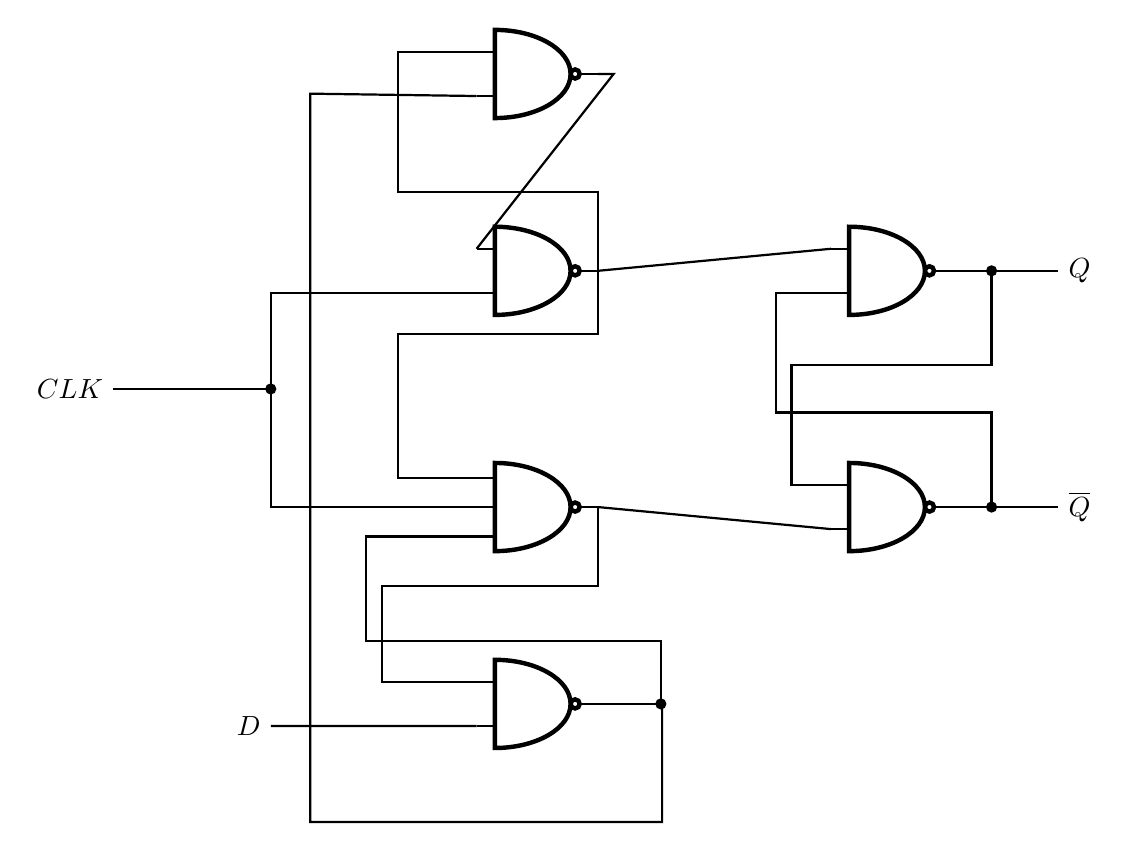
\begin{tikzpicture}[thick, >=latex, circuitikz/nand/.style={nand port, scale=1.1}]

    % ================= গেইটগুলো বসানো (Gates) =================
    % বাম দিকের ৪টি গেইট (U1 থেকে U4)
    \node[nand port, number inputs=2] (U1) at (0, 4) {};
    \node[nand port, number inputs=2] (U2) at (0, 1.5) {};
    \node[nand port, number inputs=3] (U3) at (0, -1.5) {};
    \node[nand port, number inputs=2] (U4) at (0, -4) {};

    % ডান দিকের আউটপুট ল্যাচ গেইট (U5 ও U6)
    \node[nand port, number inputs=2] (U5) at (4.5, 1.5) {};
    \node[nand port, number inputs=2] (U6) at (4.5, -1.5) {};

    % ================= ইনপুট ও আউটপুট টেক্সট =================
    \node[left] (CLK) at (-6, 0) {$CLK$};
    \node[left] (D)   at (-4, -4.28) {$D$}; 

    \node[right] (Q) at (6, 1.5) {$Q$};
    \node[right] (Qbar) at (6, -1.5) {$\overline{Q}$};

    % ================= কানেকশন (Wiring) =================

    % CLK সিগন্যাল
    \draw (CLK) -- (-4, 0) node[circ](clk_split){} |- (U2.in 2);
    \draw (clk_split) |- (U3.in 2);

    % D সিগন্যাল
    \draw (D) -- (U4.in 2);

    % U1 এর আউটপুট থেকে U2 এর টপ ইনপুট
    \draw (U1.out) -- ++(0.2,0) -- (U2.in 1);

    % U2 এর আউটপুট এবং এর ফিডব্যাক ব্রাঞ্চগুলো
    \draw (U2.out) -- (U5.in 1);
    \draw (U2.out) -- ++(0, 1) -| ([xshift=-1cm]U1.in 1) -- (U1.in 1);
    \draw (U2.out) -- ++(0, -0.8) -| ([xshift=-1cm]U3.in 1) -- (U3.in 1);

    % U3 এর আউটপুট এবং এর ফিডব্যাক ব্রাঞ্চগুলো
    \draw (U3.out) -- (U6.in 2);
    \draw (U3.out) -- ++(0, -1) -| ([xshift=-1.2cm]U4.in 1) -- (U4.in 1);

    % U4 এর আউটপুট এবং এর ফিডব্যাক ব্রাঞ্চগুলো
    \draw (U4.out) -- ++(0.8,0) node[circ](u4_out){};
    \draw (u4_out) -- ++(0, 0.8) -| ([xshift=-1.4cm]U3.in 3) -- (U3.in 3);
    \draw (U1.in 2) -- (-3.5 , 3.75) --( -3.5, -5.5 ) -- ( 0.97, -5.5 ) -- (0.97, -4);
    % U5 এবং U6 এর আউটপুট ল্যাচ ক্রস-কাপলিং
    \draw (U5.out) -- ++(0.5,0) node[circ](q_split){} -- (Q);
    \draw (U6.out) -- ++(0.5,0) node[circ](qbar_split){} -- (Qbar);

    \draw (q_split) -- ++(0, -1.2) -| ([xshift=-0.5cm]U6.in 1) -- (U6.in 1);
    \draw (qbar_split) -- ++(0, 1.2) -| ([xshift=-0.7cm]U5.in 2) -- (U5.in 2);

\end{tikzpicture}
\end{center}

\mk{6} \yr{CSE 205 | L-2/T-1 | 2015--16}


\end{enumerate}

%%──────────────────────────────────────────────────────────────────────
\subtopic{cE}{Latch vs Flip-Flop}
\label{sub:s5-latch-ff}

\begin{enumerate}

%% -- Q1: Differences between latch and flip-flop --
\item Write the differences between a latch and a flip-flop.
\mk{5} \yr{CSE 205 | L-2/T-1 | 2013--14}

\begin{tcolorbox}[enhanced,breakable,ansbox,colback=cE!4,colframe=cE,boxrule=0.8pt,arc=5pt,title={\textbf{Answer}},fonttitle=\bfseries\color{white},colbacktitle=cE]
Both latches and flip-flops are fundamental memory elements used in sequential logic circuits to store a single bit of information. However, they differ significantly in their operation, structure, and synchronization mechanics. The primary differences are detailed in the comparison table below:

\vspace{1em}
\begin{center}
\renewcommand{\arraystretch}{1.6}
\begin{tabular}{@{} p{0.22\textwidth} p{0.36\textwidth} p{0.36\textwidth} @{}}
\toprule
\textbf{Parameter} & \textbf{Latch} & \textbf{Flip-Flop} \\
\midrule
\textbf{Triggering Mechanism} & \textcolor{cE}{\textbf{Level-triggered}}: The output continuously responds to input changes as long as the Enable/Clock signal is at its active level (High or Low). & \textcolor{cE}{\textbf{Edge-triggered}}: The output responds to input changes only at a specific instant: the rising (positive) or falling (negative) edge of the clock. \\
\textbf{Structural Composition} & Simpler design; constructed directly using fundamental cross-coupled logic gates (e.g., NAND or NOR gates). & More complex design; typically constructed from a combination of latches (e.g., Master-Slave configuration) and an edge-detector circuit. \\
\textbf{Sensitivity \& Glitches} & Highly sensitive to input changes during the active level. It is vulnerable to spurious glitches if inputs fluctuate while enabled. & Inputs are sampled only precisely at the clock edge. It is highly robust and inherently immune to glitches between clock edges. \\
\textbf{Operating Speed} & Generally faster operating speeds due to shorter propagation delays through fewer logic gates. & Comparatively slower due to the propagation delays introduced by the additional circuitry required for edge-triggering. \\
\textbf{Hardware \& Area} & Requires fewer logic gates, thereby consuming less power and occupying less silicon area on an IC. & Requires more logic gates, leading to higher power consumption and a larger silicon footprint. \\
\textbf{Usage \& Applications} & Best suited for asynchronous sequential circuits, simple buffers, and designs where strict timing synchronization is not critical. & The fundamental building block for synchronous sequential circuits, shift registers, counters, and microprocessor state machines. \\
\bottomrule
\end{tabular}
\end{center}

\vspace{1em}
\textbf{Conceptual Analogy:}
\begin{itemize}
    \item A \textbf{Latch} behaves like a \textcolor{cE}{transparent window}: as long as the window is open (enable is active), everything passing by outside (inputs) is immediately seen inside (outputs).
    \item A \textbf{Flip-Flop} behaves like a \textcolor{cE}{camera shutter}: it captures a frozen snapshot of the outside (inputs) only at the exact fraction of a second the shutter clicks (clock edge), ignoring changes before and after.
\end{itemize}
\end{tcolorbox}

\end{enumerate}

%%──────────────────────────────────────────────────────────────────────
\subtopic{cE}{Flip-Flop Conversion}
\label{sub:s5-conversion}

\begin{enumerate}

\item Design a T flip-flop using a JK flip-flop and verify its operation using state transitions.
\mk{10} \yr{CSE 205 | L-2/T-1 | 2024--25}

\begin{tcolorbox}[enhanced,breakable,ansbox,colback=cE!4,colframe=cE,boxrule=0.8pt,arc=5pt,title={\textbf{Answer}},fonttitle=\bfseries\color{white},colbacktitle=cE]
To design a \textbf{T (Toggle) flip-flop} using a \textbf{JK flip-flop}, we must determine how to drive the $J$ and $K$ inputs such that the JK flip-flop mimics the behavior of a T flip-flop. We begin by comparing their excitation tables.

\subsubsection*{1. Excitation Table Formulation}
The T flip-flop has a single input $T$ which toggles the state when $T=1$ and retains the state when $T=0$. The JK flip-flop requires specific $J$ and $K$ inputs to achieve these identical state transitions ($Q_n \rightarrow Q_{n+1}$).

\begin{center}
\renewcommand{\arraystretch}{1.2}
\begin{tabular}{@{} cc | c || cc @{}}
\toprule
\multicolumn{2}{c|}{\textbf{State Transition}} & \textbf{T Flip-Flop} & \multicolumn{2}{c}{\textbf{JK Flip-Flop Inputs}} \\
$Q_n$ (Current) & $Q_{n+1}$ (Next) & Required $T$ & Required $J$ & Required $K$ \\
\midrule
0 & 0 & 0 & 0 & X \\
0 & 1 & 1 & 1 & X \\
1 & 0 & 1 & X & 1 \\
1 & 1 & 0 & X & 0 \\
\bottomrule
\end{tabular}
\end{center}
\textit{Note: 'X' denotes a "Don't Care" condition.}

\subsubsection*{2. Boolean Expression Derivation}
By observing the table above, we can directly derive the Boolean expressions for inputs $J$ and $K$ in terms of $T$:
\begin{itemize}
    \item For the \textbf{J input}: Looking at the rows where $J$ is not 'X' (rows 1 and 2), we see that $J = 0$ when $T = 0$, and $J = 1$ when $T = 1$. Thus, \textcolor{cE}{$\mathbf{J = T}$}.
    \item For the \textbf{K input}: Looking at the rows where $K$ is not 'X' (rows 3 and 4), we see that $K = 1$ when $T = 1$, and $K = 0$ when $T = 0$. Thus, \textcolor{cE}{$\mathbf{K = T}$}.
\end{itemize}

Since $J = T$ and $K = T$, we simply tie the $J$ and $K$ inputs of the JK flip-flop together and connect them to the $T$ input.

\subsubsection*{3. Logic Circuit Diagram}
\begin{center}
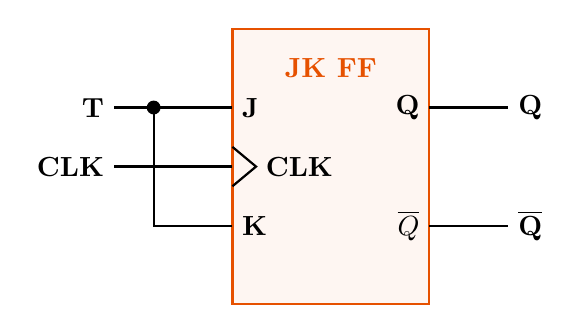
\begin{tikzpicture}
    % Draw the JK Flip-Flop Block
    \draw[thick, fill=cE!5, draw=cE] (0,0) rectangle (2.5,3.5);
    \node[font=\bfseries, text=cE] at (1.25, 3) {JK FF};
    
    % Clock Edge Symbol
    \draw[thick] (0, 1.5) -- (0.3, 1.75) -- (0, 2);
    
    % Pin Labels Inside the FF
    \node[right, font=\bfseries] at (0, 2.5) {J};
    \node[right, font=\bfseries] at (0.3, 1.75) {CLK};
    \node[right, font=\bfseries] at (0, 1) {K};
    
    \node[left, font=\bfseries] at (2.5, 2.5) {Q};
    \node[left, font=\bfseries] at (2.5, 1) {$\overline{Q}$};
    
    % Input Connections
    \draw[thick] (-1.5, 2.5) node[left] {\textbf{T}} -- (0, 2.5);
    \draw[thick] (-1, 2.5) |- (0, 1);
    \fill (-1, 2.5) circle (2.5pt); % Junction dot
    
    % Clock Connection
    \draw[thick] (-1.5, 1.75) node[left] {\textbf{CLK}} -- (0, 1.75);
    
    % Output Connections
    \draw[thick] (2.5, 2.5) -- (3.5, 2.5) node[right] {\textbf{Q}};
    \draw[thick] (2.5, 1) -- (3.5, 1) node[right] {$\mathbf{\overline{Q}}$};
\end{tikzpicture}
\end{center}

\subsubsection*{4. Mathematical Verification via State Transitions}
To verify the operation mathematically, we analyze the characteristic equation of a standard JK flip-flop:
\begin{align*}
    Q_{n+1} &= J\overline{Q_n} + \overline{K}Q_n \quad &&\text{(Characteristic equation of JK FF)} \\
    \intertext{Substitute the derived relationships $J = T$ and $K = T$:}
    Q_{n+1} &= T\overline{Q_n} + \overline{T}Q_n \quad &&\text{(Substitution)} \\
    Q_{n+1} &= T \oplus Q_n \quad &&\text{(Definition of XOR operation)}
\end{align*}
The resulting equation, \textcolor{cE}{$\mathbf{Q_{n+1} = T \oplus Q_n}$}, is exactly the characteristic equation of a T flip-flop. 

\textbf{Conclusion:} 
\begin{itemize}
    \item When $T = 0 \implies Q_{n+1} = 0 \oplus Q_n = Q_n$ (The state is \textbf{Held}).
    \item When $T = 1 \implies Q_{n+1} = 1 \oplus Q_n = \overline{Q_n}$ (The state is \textbf{Toggled}).
\end{itemize}
This logically confirms that tying the $J$ and $K$ inputs together creates a fully functional T flip-flop.
\end{tcolorbox}

\item Construct a JK flip-flop using a T flip-flop and basic gates.
\mk{6} \yr{CSE 205 | L-2/T-1 | 2023--24}

\begin{tcolorbox}[enhanced,breakable,ansbox,colback=cE!4,colframe=cE,boxrule=0.8pt,arc=5pt,title={\textbf{Answer}},fonttitle=\bfseries\color{white},colbacktitle=cE]
To design a \textbf{JK flip-flop} using a \textbf{T flip-flop} and basic logic gates, we must determine the combinational logic required at the $T$ input. This logic must translate the $J$, $K$, and current state ($Q_n$) into the appropriate toggle signal ($T$) so that the flip-flop mimics the transitions of a JK flip-flop.

\subsubsection*{1. Conversion Table Formulation}
We begin by establishing the required state transitions for a JK flip-flop and using the excitation table of a T flip-flop to determine the necessary $T$ input. 
\begin{itemize}
    \item \textbf{T Flip-Flop Excitation Rule:} $T = Q_n \oplus Q_{n+1}$ (i.e., $T=1$ if the state changes, $T=0$ if it remains the same).
\end{itemize}

\begin{center}
\renewcommand{\arraystretch}{1.2}
\begin{tabular}{@{} ccc | c || c @{}}
\toprule
\multicolumn{3}{c|}{\textbf{JK Flip-Flop Inputs \& State}} & \textbf{Next State} & \textbf{Required T Input} \\
$J$ & $K$ & $Q_n$ (Current) & $Q_{n+1}$ (Target) & $T$ ($Q_n \oplus Q_{n+1}$) \\
\midrule
0 & 0 & 0 & 0 & 0 \\
0 & 0 & 1 & 1 & 0 \\
0 & 1 & 0 & 0 & 0 \\
0 & 1 & 1 & 0 & 1 \\
1 & 0 & 0 & 1 & 1 \\
1 & 0 & 1 & 1 & 0 \\
1 & 1 & 0 & 1 & 1 \\
1 & 1 & 1 & 0 & 1 \\
\bottomrule
\end{tabular}
\end{center}

\subsubsection*{2. Boolean Mathematical Derivation}
From the conversion table, we can write the standard Sum-of-Products (SOP) expression for $T(J, K, Q_n)$ by identifying the rows where $T = 1$:
\begin{align*}
    T &= \Sigma m(3, 4, 6, 7) \\
    T &= \overline{J}K Q_n + J\overline{K}\overline{Q_n} + JK\overline{Q_n} + JKQ_n \quad &&\text{(Standard SOP form)}
\end{align*}

Now, we perform step-by-step Boolean simplification:
\begin{align*}
    T &= J\overline{K}\overline{Q_n} + JK\overline{Q_n} + \overline{J}KQ_n + JKQ_n \quad &&\text{(Commutative Law - Grouping terms)} \\
    T &= J\overline{Q_n}(\overline{K} + K) + KQ_n(\overline{J} + J) \quad &&\text{(Distributive Law)} \\
    T &= J\overline{Q_n}(1) + KQ_n(1) \quad &&\text{(Complementarity Law: } A + \overline{A} = 1 \text{)} \\
    \textcolor{cE}{\mathbf{T}} &\textcolor{cE}{\mathbf{= J\overline{Q_n} + KQ_n}} \quad &&\text{(Identity Law)}
\end{align*}

\textit{Alternative Verification via Characteristic Equations:}
\begin{align*}
    Q_{n+1} (\text{T FF}) &= T \oplus Q_n \\
    Q_{n+1} (\text{JK FF}) &= J\overline{Q_n} + \overline{K}Q_n \\
    \text{Equating the two: } T \oplus Q_n &= J\overline{Q_n} + \overline{K}Q_n \\
    \text{XORing both sides by } Q_n: T &= (J\overline{Q_n} + \overline{K}Q_n) \oplus Q_n \\
    T &= (J\overline{Q_n} + \overline{K}Q_n)\overline{Q_n} + \overline{(J\overline{Q_n} + \overline{K}Q_n)}Q_n \quad &&\text{(XOR Expansion)} \\
    T &= J\overline{Q_n} + (\overline{J} + Q_n)(K + \overline{Q_n})Q_n \quad &&\text{(De Morgan's \& ANDing)} \\
    T &= J\overline{Q_n} + (\overline{J}K + \overline{J}\overline{Q_n} + KQ_n + 0)Q_n \quad &&\text{(Distributive Law)} \\
    T &= J\overline{Q_n} + \overline{J}KQ_n + 0 + KQ_n \quad &&\text{(Idempotent \& Annulment)} \\
    T &= J\overline{Q_n} + KQ_n(\overline{J} + 1) = J\overline{Q_n} + KQ_n \quad &&\text{(Absorption Law)}
\end{align*}
Both approaches yield the exact same required combinational logic for $T$.

\vspace{1em}
\subsubsection*{3. Logic Circuit Realization}
Based on the derived equation \textcolor{cE}{$\mathbf{T = J\overline{Q_n} + KQ_n}$}, the circuit requires:
\begin{itemize}
    \item One T Flip-Flop.
    \item Two 2-input AND gates (to compute $J \cdot \overline{Q_n}$ and $K \cdot Q_n$).
    \item One 2-input OR gate (to sum the products).
\end{itemize}

\begin{center}
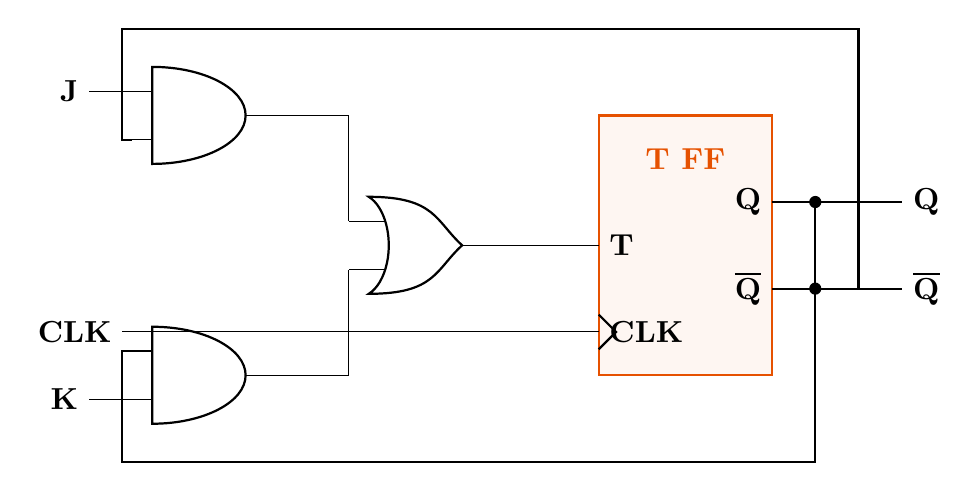
\begin{tikzpicture}[scale=1.1, transform shape]
    % T flip flop block
    \draw[thick, fill=cE!5, draw=cE] (5,-1.5) rectangle (7,1.5);
    \node[font=\bfseries, text=cE] at (6, 1) {T FF};
    
    % Pins inside T FF
    \node[right, font=\bfseries] at (5, 0) {T};
    \node[right, font=\bfseries] at (5, -1) {CLK};
    \node[left, font=\bfseries] at (7, 0.5) {Q};
    \node[left, font=\bfseries] at (7, -0.5) {$\overline{\text{Q}}$};
    
    % Clock Edge Symbol
    \draw[thick] (5,-0.8) -- (5.2,-1) -- (5,-1.2);
    
    % Logic gates
    \node[and port] (and1) at (1, 1.5) {};
    \node[and port] (and2) at (1, -1.5) {};
    \node[or port] (or1) at (3.5, 0) {};
    
    % Input Labels (J, K)
    \draw (and1.in 1) -- ++(-0.5,0) node[left] {\textbf{J}};
    \draw (and2.in 2) -- ++(-0.5,0) node[left] {\textbf{K}};
    
    % Connections from ANDs to OR
    \draw (and1.out) -| (or1.in 1);
    \draw (and2.out) -| (or1.in 2);
    \draw (or1.out) -- (5,0); % OR out to T input
    
    % Feedback Connection: Qbar to AND1 (J * Qbar)
    \draw[thick] (7, -0.5) -- (8, -0.5) -- (8, 2.5) -- (-0.5, 2.5) |- (and1.in 2);
    \fill (7.5, -0.5) circle (2pt); % Junction dot for Qbar wire
    
    % Feedback Connection: Q to AND2 (K * Q)
    \draw[thick] (7, 0.5) -- (7.5, 0.5) -- (7.5, -2.5) -- (-0.5, -2.5) |- (and2.in 1);
    \fill (7, 0.5) ++(0.5,0) circle (2pt); % Junction dot for Q wire
    
    % Output wire extensions
    \draw[thick] (7, 0.5) -- (8.5, 0.5) node[right] {\textbf{Q}};
    \draw[thick] (7, -0.5) -- (8.5, -0.5) node[right] {$\mathbf{\overline{Q}}$};
    
    % Clock Connection
    \draw (5,-1) -- ++(-5.5,0) node[left] {\textbf{CLK}};
\end{tikzpicture}
\end{center}
\end{tcolorbox}

\item Construct a JK flip-flop from a T flip-flop and necessary gates. Show all the steps of this construction process.
\mk{11} \yr{CSE 205 | L-2/T-1 | 2022--23}

\begin{tcolorbox}[enhanced,breakable,ansbox,colback=cE!4,colframe=cE,boxrule=0.8pt,arc=5pt,title={\textbf{Answer}},fonttitle=\bfseries\color{white},colbacktitle=cE]
To construct a \textbf{JK flip-flop} (the target) using a \textbf{T flip-flop} (the available hardware) and basic logic gates, we must design a combinational circuit that generates the appropriate $T$ input based on the $J$ and $K$ inputs and the current state $Q_n$. 

The construction process follows a systematic four-step methodology:

\subsubsection*{Step 1: Define Target and Available Flip-Flop Characteristics}
First, we state the excitation requirement for the available \textbf{T flip-flop} and the state transition behavior of the target \textbf{JK flip-flop}.
\begin{itemize}
    \item \textbf{T Flip-Flop Excitation:} To change state ($Q_{n+1} = \overline{Q_n}$), we need $T = 1$. To hold state ($Q_{n+1} = Q_n$), we need $T = 0$. Mathematically, $T = Q_n \oplus Q_{n+1}$.
    \item \textbf{JK Flip-Flop Behavior:} $Q_{n+1} = J\overline{Q_n} + \overline{K}Q_n$.
\end{itemize}

\subsubsection*{Step 2: Construct the Conversion Table}
We merge the characteristic table of the JK flip-flop with the excitation requirements of the T flip-flop to determine the required $T$ input for every combination of $J$, $K$, and $Q_n$.

\begin{center}
\renewcommand{\arraystretch}{1.2}
\begin{tabular}{@{} ccc | c || c @{}}
\toprule
\multicolumn{3}{c|}{\textbf{Target JK Inputs \& State}} & \textbf{Next State} & \textbf{Required Input} \\
$J$ & $K$ & $Q_n$ (Current) & $Q_{n+1}$ & $T = Q_n \oplus Q_{n+1}$ \\
\midrule
0 & 0 & 0 & 0 & \textcolor{cE}{\textbf{0}} \\
0 & 0 & 1 & 1 & \textcolor{cE}{\textbf{0}} \\
0 & 1 & 0 & 0 & \textcolor{cE}{\textbf{0}} \\
0 & 1 & 1 & 0 & \textcolor{cE}{\textbf{1}} \\
1 & 0 & 0 & 1 & \textcolor{cE}{\textbf{1}} \\
1 & 0 & 1 & 1 & \textcolor{cE}{\textbf{0}} \\
1 & 1 & 0 & 1 & \textcolor{cE}{\textbf{1}} \\
1 & 1 & 1 & 0 & \textcolor{cE}{\textbf{1}} \\
\bottomrule
\end{tabular}
\end{center}

\subsubsection*{Step 3: Boolean Simplification using Karnaugh Map}
From the conversion table, the minterms for $T$ are $m(3, 4, 6, 7)$. We plot these on a 3-variable Karnaugh Map to find the minimized Sum-of-Products (SOP) expression for $T$.

\begin{center}
\begin{karnaugh-map}[4][2][1][$KQ_n$][$J$]
    \minterms{3,4,6,7}
    \maxterms{0,1,2,5}
    \implicantedge{4}{4}{6}{6} % Correct wrap-around grouping for J\bar{Q_n}
    \implicant{3}{7} 
\end{karnaugh-map}
\end{center}

\textbf{Groupings:}
\begin{itemize}
    \item The horizontal pair covering cells 4 and 6 yields the term: \textcolor{cE}{$J\overline{Q_n}$}
    \item The vertical pair covering cells 3 and 7 yields the term: \textcolor{cE}{$KQ_n$}
\end{itemize}
Applying the OR operation to these prime implicants provides the final combinational logic equation:
\begin{align*}
    \textcolor{cE}{\mathbf{T}} &\textcolor{cE}{\mathbf{= J\overline{Q_n} + KQ_n}}
\end{align*}

\subsubsection*{Step 4: Logic Circuit Implementation}
Using the derived Boolean equation, the combinational logic requires two AND gates and one OR gate. The outputs of the flip-flop ($Q$ and $\overline{Q}$) are fed back into the AND gates to evaluate the current state.

\vspace{1em}
\begin{center}
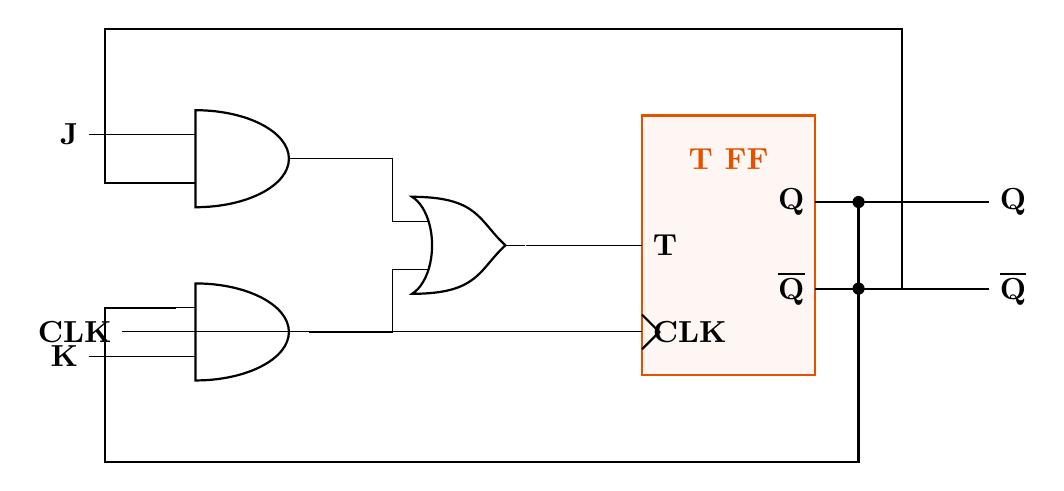
\begin{tikzpicture}[scale=1.1, transform shape]
    % T flip flop block
    \draw[thick, fill=cE!5, draw=cE] (5,-1.5) rectangle (7,1.5);
    \node[font=\bfseries, text=cE] at (6, 1) {T FF};
    
    % Pins inside T FF
    \node[right, font=\bfseries] at (5, 0) {T};
    \node[right, font=\bfseries] at (5, -1) {CLK};
    \node[left, font=\bfseries] at (7, 0.5) {Q};
    \node[left, font=\bfseries] at (7, -0.5) {$\overline{\text{Q}}$};
    
    % Clock Edge Symbol
    \draw[thick] (5,-0.8) -- (5.2,-1) -- (5,-1.2);
    
    % Logic gates
    \node[and port] (and1) at (1, 1) {};
    \node[and port] (and2) at (1, -1) {};
    \node[or port] (or1) at (3.5, 0) {};
    
    % Input Labels (J, K)
    \draw (and1.in 1) -- ++(-1,0) node[left] {\textbf{J}};
    \draw (and2.in 2) -- ++(-1,0) node[left] {\textbf{K}};
    
    % Connections from ANDs to OR
    \draw (and1.out) -| (or1.in 1);
    \draw (and2.out) -| (or1.in 2);
    \draw (or1.out) -- (5,0); % OR out to T input
    
    % Feedback Connection: Qbar to AND1 (J * Qbar)
    \draw[thick] (7, -0.5) -- (8, -0.5) -- (8, 2.5) -- (-1.2, 2.5) |- (and1.in 2);
    \fill (7.5, -0.5) circle (2pt); % Junction dot for Qbar wire
    
    % Feedback Connection: Q to AND2 (K * Q)
    \draw[thick] (7, 0.5) -- (7.5, 0.5) -- (7.5, -2.5) -- (-1.2, -2.5) |- (and2.in 1);
    \fill (7.5, 0.5) circle (2pt); % Junction dot for Q wire
    
    % Output wire extensions
    \draw[thick] (7, 0.5) -- (9, 0.5) node[right] {\textbf{Q}};
    \draw[thick] (7, -0.5) -- (9, -0.5) node[right] {$\mathbf{\overline{Q}}$};
    
    % Clock Connection
    \draw (5,-1) -- ++(-6,0) node[left] {\textbf{CLK}};
\end{tikzpicture}
\end{center}
\end{tcolorbox}

\item Design a D flip-flop using a T flip-flop and gates.
\mk{5} \yr{CSE 205 | L-2/T-1 | 2020--21}
\variant{2019--20}

\begin{tcolorbox}[enhanced,breakable,ansbox,colback=cE!4,colframe=cE,boxrule=0.8pt,arc=5pt,title={\textbf{Answer}},fonttitle=\bfseries\color{white},colbacktitle=cE]
To design a \textbf{D flip-flop} (target) using a \textbf{T flip-flop} (available hardware) and basic logic gates, we must design a combinational circuit that determines the appropriate $T$ input based on the target $D$ input and the current state $Q_n$.

\subsubsection*{1. Excitation and Conversion Table Formulation}
We begin by establishing the required state transitions for a D flip-flop and mapping them to the excitation requirements of a T flip-flop.
\begin{itemize}
    \item \textbf{D Flip-Flop Target Behavior:} The next state simply follows the input, meaning $Q_{n+1} = D$.
    \item \textbf{T Flip-Flop Excitation Rule:} The input $T$ must be $1$ to toggle the state ($Q_n \neq Q_{n+1}$), and $0$ to hold the state ($Q_n = Q_{n+1}$). Mathematically, $T = Q_n \oplus Q_{n+1}$.
\end{itemize}

\begin{center}
\renewcommand{\arraystretch}{1.2}
\begin{tabular}{@{} cc | c || c @{}}
\toprule
\multicolumn{2}{c|}{\textbf{Target D Input \& State}} & \textbf{Next State} & \textbf{Required T Input} \\
$D$ & $Q_n$ (Current) & $Q_{n+1}$ (Target, $=D$) & $T = Q_n \oplus Q_{n+1}$ \\
\midrule
0 & 0 & 0 & \textcolor{cE}{\textbf{0}} \\
0 & 1 & 0 & \textcolor{cE}{\textbf{1}} \\
1 & 0 & 1 & \textcolor{cE}{\textbf{1}} \\
1 & 1 & 1 & \textcolor{cE}{\textbf{0}} \\
\bottomrule
\end{tabular}
\end{center}

\subsubsection*{2. Boolean Expression Derivation}
From the conversion table, we can directly write the Sum-of-Products (SOP) expression for the required $T$ input by identifying the rows where $T = 1$:
\begin{align*}
    T &= \Sigma m(1, 2) \\
    T &= \overline{D}Q_n + D\overline{Q_n} \quad &&\text{(Standard SOP form extracted from the table)} \\
    \textcolor{cE}{\mathbf{T}} &\textcolor{cE}{\mathbf{= D \oplus Q_n}} \quad &&\text{(Definition of the XOR operation)}
\end{align*}

\textit{Alternative Algebraic Verification:}
\begin{align*}
    Q_{n+1} \text{ (T FF)} &= T \oplus Q_n \quad &&\text{(Characteristic equation of T FF)} \\
    \text{Substitute } T &= D \oplus Q_n : \\
    Q_{n+1} &= (D \oplus Q_n) \oplus Q_n \quad &&\text{(Substitution)} \\
    Q_{n+1} &= D \oplus (Q_n \oplus Q_n) \quad &&\text{(Associative Law of XOR)} \\
    Q_{n+1} &= D \oplus 0 \quad &&\text{(Self-Inverse Law: } A \oplus A = 0\text{)} \\
    Q_{n+1} &= D \quad &&\text{(Identity Law of XOR: } A \oplus 0 = A\text{)}
\end{align*}
This confirms that driving the $T$ input with $D \oplus Q_n$ flawlessly replicates the behavior of a D flip-flop ($Q_{n+1} = D$).

\vspace{1em}
\subsubsection*{3. Logic Circuit Realization}
Based on the derived equation \textcolor{cE}{$\mathbf{T = D \oplus Q_n}$}, the circuit requires only a single 2-input XOR gate connected to the $T$ input. The current state output $Q$ is fed back to serve as one of the inputs to this XOR gate.

\begin{center}
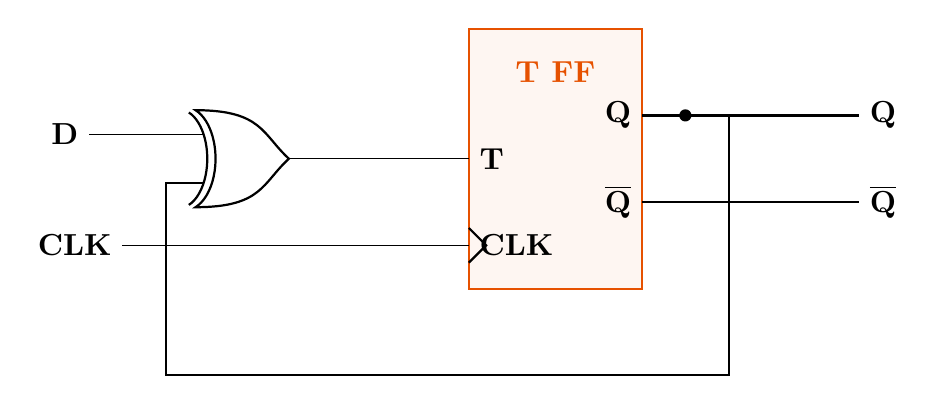
\begin{tikzpicture}[scale=1.1, transform shape]
    % T flip flop block
    \draw[thick, fill=cE!5, draw=cE] (4,-1.5) rectangle (6,1.5);
    \node[font=\bfseries, text=cE] at (5, 1) {T FF};
    
    % Pins inside T FF
    \node[right, font=\bfseries] at (4, 0) {T};
    \node[right, font=\bfseries] at (4, -1) {CLK};
    \node[left, font=\bfseries] at (6, 0.5) {Q};
    \node[left, font=\bfseries] at (6, -0.5) {$\overline{\text{Q}}$};
    
    % Clock Edge Symbol
    \draw[thick] (4,-0.8) -- (4.2,-1) -- (4,-1.2);
    
    % Logic gates
    \node[xor port] (xor1) at (2, 0) {};
    
    % Input Labels (D)
    \draw (xor1.in 1) -- ++(-1,0) node[left] {\textbf{D}};
    
    % Connections from XOR to T
    \draw (xor1.out) -- (4,0); 
    
    % Feedback Connection: Q to XOR input 2 (Q_n)
    \draw[thick] (6, 0.5) -- (7, 0.5) -- (7, -2.5) -- (0.5, -2.5) |- (xor1.in 2);
    \fill (6.5, 0.5) circle (2pt); % Junction dot for Q wire
    
    % Output wire extensions
    \draw[thick] (6, 0.5) -- (8.5, 0.5) node[right] {\textbf{Q}};
    \draw[thick] (6, -0.5) -- (8.5, -0.5) node[right] {$\mathbf{\overline{Q}}$};
    
    % Clock Connection
    \draw (4,-1) -- ++(-4,0) node[left] {\textbf{CLK}};
\end{tikzpicture}
\end{center}
\end{tcolorbox}

\item Design a JK Flip-Flop using a T Flip-Flop and basic gates.
\mk{10} \yr{CSE 205 | L-2/T-1 | 2016--17}

\begin{tcolorbox}[enhanced,breakable,ansbox,colback=cE!4,colframe=cE,boxrule=0.8pt,arc=5pt,title={\textbf{Answer}},fonttitle=\bfseries\color{white},colbacktitle=cE]
To design a \textbf{JK flip-flop} (the target device) using a \textbf{T flip-flop} (the available device) and basic logic gates, we must design a combinational logic circuit that determines the required $T$ input based on the external $J$ and $K$ inputs as well as the current state $Q_n$.

\subsubsection*{1. Excitation and Conversion Table}
First, we determine the required state transitions for a JK flip-flop and map them to the corresponding excitation requirements of a T flip-flop.
\begin{itemize}
    \item \textbf{JK Flip-Flop Target Behavior:} $Q_{n+1} = J\overline{Q_n} + \overline{K}Q_n$
    \item \textbf{T Flip-Flop Excitation Rule:} To change state, $T=1$. To hold state, $T=0$. Mathematically, $T = Q_n \oplus Q_{n+1}$.
\end{itemize}

\begin{center}
\renewcommand{\arraystretch}{1.2}
\begin{tabular}{@{} ccc | c || c @{}}
\toprule
\multicolumn{3}{c|}{\textbf{External Inputs \& Current State}} & \textbf{Next State} & \textbf{Required T Input} \\
$J$ & $K$ & $Q_n$ & $Q_{n+1}$ & $T = Q_n \oplus Q_{n+1}$ \\
\midrule
0 & 0 & 0 & 0 & \textcolor{cE}{\textbf{0}} \\
0 & 0 & 1 & 1 & \textcolor{cE}{\textbf{0}} \\
0 & 1 & 0 & 0 & \textcolor{cE}{\textbf{0}} \\
0 & 1 & 1 & 0 & \textcolor{cE}{\textbf{1}} \\
1 & 0 & 0 & 1 & \textcolor{cE}{\textbf{1}} \\
1 & 0 & 1 & 1 & \textcolor{cE}{\textbf{0}} \\
1 & 1 & 0 & 1 & \textcolor{cE}{\textbf{1}} \\
1 & 1 & 1 & 0 & \textcolor{cE}{\textbf{1}} \\
\bottomrule
\end{tabular}
\end{center}

\subsubsection*{2. Boolean Simplification using Karnaugh Map}
From the conversion table, the minterms for which $T = 1$ are $m(3, 4, 6, 7)$. We plot these on a 3-variable Karnaugh Map to find the minimized expression for $T(J, K, Q_n)$.

\begin{center}
\begin{karnaugh-map}[4][2][1][$KQ_n$][$J$]
    \minterms{3,4,6,7}
    \maxterms{0,1,2,5}
    \implicantedge{4}{4}{6}{6} % Correct wrap-around grouping for J\bar{Q_n}
    \implicant{3}{7}           % Vertical grouping for KQ_n
\end{karnaugh-map}
\end{center}

\textbf{Groupings \& Derivation:}
\begin{align*}
    \text{Horizontal Pair (Cells 4, 6)} &\implies J\overline{Q_n} \\
    \text{Vertical Pair (Cells 3, 7)} &\implies KQ_n \\
    \intertext{Applying the logical OR to these prime implicants provides the final minimal equation:}
    \textcolor{cE}{\mathbf{T}} &\textcolor{cE}{\mathbf{= J\overline{Q_n} + KQ_n}}
\end{align*}

\subsubsection*{3. Logic Circuit Realization}
The derived Boolean equation indicates that the input to the T flip-flop must be driven by an AND-OR logic structure. Specifically, we require:
\begin{itemize}
    \item Two 2-input AND gates (for $J\overline{Q_n}$ and $KQ_n$).
    \item One 2-input OR gate to sum the product terms.
    \item Feedback connections from the outputs $Q$ and $\overline{Q}$ to the inputs of the AND gates.
\end{itemize}

\vspace{1em}
\begin{center}
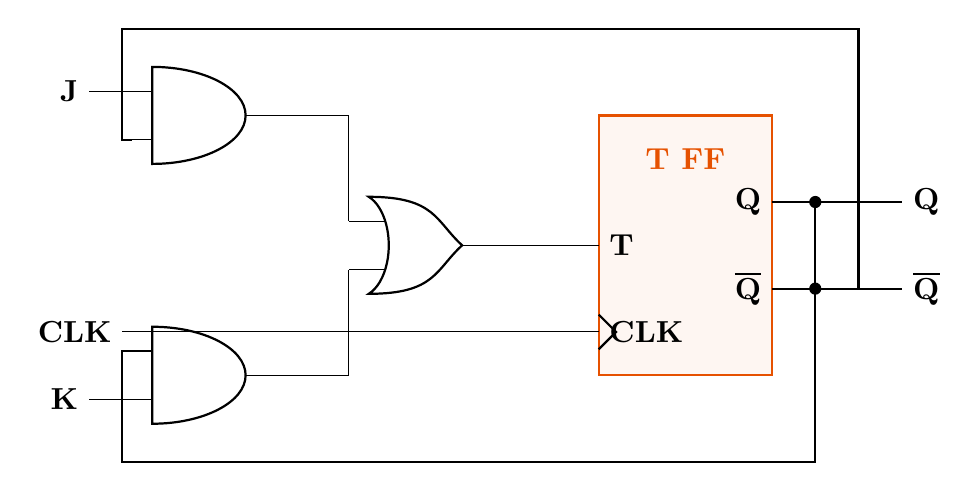
\begin{tikzpicture}[scale=1.1, transform shape]
    % T flip flop block
    \draw[thick, fill=cE!5, draw=cE] (5,-1.5) rectangle (7,1.5);
    \node[font=\bfseries, text=cE] at (6, 1) {T FF};
    
    % Pins inside T FF
    \node[right, font=\bfseries] at (5, 0) {T};
    \node[right, font=\bfseries] at (5, -1) {CLK};
    \node[left, font=\bfseries] at (7, 0.5) {Q};
    \node[left, font=\bfseries] at (7, -0.5) {$\overline{\text{Q}}$};
    
    % Clock Edge Symbol
    \draw[thick] (5,-0.8) -- (5.2,-1) -- (5,-1.2);
    
    % Logic gates
    \node[and port] (and1) at (1, 1.5) {};
    \node[and port] (and2) at (1, -1.5) {};
    \node[or port] (or1) at (3.5, 0) {};
    
    % Input Labels (J, K)
    \draw (and1.in 1) -- ++(-0.5,0) node[left] {\textbf{J}};
    \draw (and2.in 2) -- ++(-0.5,0) node[left] {\textbf{K}};
    
    % Connections from ANDs to OR
    \draw (and1.out) -| (or1.in 1);
    \draw (and2.out) -| (or1.in 2);
    \draw (or1.out) -- (5,0); % OR out to T input
    
    % Feedback Connection: Qbar to AND1 (J * Qbar)
    \draw[thick] (7, -0.5) -- (8, -0.5) -- (8, 2.5) -- (-0.5, 2.5) |- (and1.in 2);
    \fill (7.5, -0.5) circle (2pt); % Junction dot for Qbar wire
    
    % Feedback Connection: Q to AND2 (K * Q)
    \draw[thick] (7, 0.5) -- (7.5, 0.5) -- (7.5, -2.5) -- (-0.5, -2.5) |- (and2.in 1);
    \fill (7, 0.5) ++(0.5,0) circle (2pt); % Junction dot for Q wire
    
    % Output wire extensions
    \draw[thick] (7, 0.5) -- (8.5, 0.5) node[right] {\textbf{Q}};
    \draw[thick] (7, -0.5) -- (8.5, -0.5) node[right] {$\mathbf{\overline{Q}}$};
    
    % Clock Connection
    \draw (5,-1) -- ++(-5.5,0) node[left] {\textbf{CLK}};
\end{tikzpicture}
\end{center}
\end{tcolorbox}

\item Design a SR Flip-Flop using a D Flip-Flop and a $4\times1$ MUX.
\mk{10} \yr{CSE 205 | L-2/T-1 | 2014--15}

\begin{tcolorbox}[enhanced,breakable,ansbox,colback=cE!4,colframe=cE,boxrule=0.8pt,arc=5pt,title={\textbf{Answer}},fonttitle=\bfseries\color{white},colbacktitle=cE]

\textbf{1. Design Objective} \\
To design a Synchronous SR Flip-Flop using a single D Flip-Flop and a $4\times1$ Multiplexer (MUX). 

\textbf{2. Characteristic Equations} \\
The relationship between the present state ($Q_n$), next state ($Q_{n+1}$), and the inputs determines the behavior of the flip-flops:
\begin{itemize}
    \item \textbf{D Flip-Flop:} The next state simply follows the D input. 
    \begin{align*}
        Q_{n+1} &= D
    \end{align*}
    \item \textbf{SR Flip-Flop:} The next state is defined by the $S$ (Set) and $R$ (Reset) inputs. The state equation is:
    \begin{align*}
        Q_{n+1} &= S + \overline{R}Q_n \quad \text{(Valid when } SR = 0\text{)}
    \end{align*}
\end{itemize}
Because $Q_{n+1} = D$, the required D input at any time is exactly the required next state of the SR flip-flop. We can use the $4\times1$ MUX to implement this next-state logic.

\vspace{1em}
\textbf{3. Truth Table \& MUX Implementation Logic}
We will use the $S$ and $R$ inputs as the selection lines for the $4\times1$ MUX. Let $S_1 = S$ and $S_0 = R$. The MUX will select one of its four data inputs ($I_0, I_1, I_2, I_3$) and route it to the output $Y$, which is connected to the $D$ input of the flip-flop.

The logical function of the $4\times1$ MUX is:
\begin{align*}
    Y &= \overline{S_1}\overline{S_0}I_0 + \overline{S_1}S_0I_1 + S_1\overline{S_0}I_2 + S_1S_0I_3
\end{align*}

Let's derive the inputs $I_0$ to $I_3$ from the SR Flip-Flop characteristic table:

\begin{center}
\renewcommand{\arraystretch}{1.3}
\begin{tabular}{cc|c|c|l}
\toprule
\multicolumn{2}{c|}{\textbf{Select Lines}} & \textbf{Next State} & \textbf{Required Input} & \textbf{MUX Data Input} \\
$S$ ($S_1$) & $R$ ($S_0$) & $Q_{n+1}$ & $D = Q_{n+1}$ & \textbf{Assignment} \\
\midrule
$0$ & $0$ & $Q_n$ (Hold)  & $Q_n$ & $I_0 = Q_n$ \\
$0$ & $1$ & $0$ (Reset) & $0$ & $I_1 = 0$ \\
$1$ & $0$ & $1$ (Set)   & $1$ & $I_2 = 1$ \\
$1$ & $1$ & $X$ (Invalid) & $0$ (or $X$) & $I_3 = 0$ \quad \textit{(Grounding to avoid floating state)} \\
\bottomrule
\end{tabular}
\end{center}

Substituting these inputs into the MUX equation gives us the exact D input required:
\begin{align*}
    D &= \overline{S}\overline{R}(Q_n) + \overline{S}R(0) + S\overline{R}(1) + SR(0) \\
    D &= \overline{S}\overline{R}Q_n + S\overline{R}
\end{align*}
\textit{Note: This simplifies to $S + \overline{R}Q_n$, which perfectly matches the SR flip-flop characteristic equation.}

\vspace{1em}
\textbf{4. Circuit Diagram} \\
The circuit below visualizes the implementation. The $4\times1$ MUX generates the next-state logic based on $S$ and $R$, feeding into the D Flip-Flop. The present state output $Q$ is fed back into the $I_0$ input of the MUX to enable the "Hold" state.

\begin{center}
\begin{circuitikz}[scale=1.1, transform shape]
    % 4x1 MUX Node (Drawn manually for precise input/output mapping)
    \draw[thick, fill=cE!10] (0,0) rectangle (2,4);
    \node[font=\bfseries\large, text=cE] at (1, 2) {MUX};
    \node[right, font=\small] at (0, 3.4) {$I_0$};
    \node[right, font=\small] at (0, 2.6) {$I_1$};
    \node[right, font=\small] at (0, 1.8) {$I_2$};
    \node[right, font=\small] at (0, 1.0) {$I_3$};
    \node[left, font=\small] at (2, 2.2) {$Y$};
    \node[above, font=\small] at (0.6, 0) {$S_1$};
    \node[above, font=\small] at (1.4, 0) {$S_0$};
    \node[above, font=\bfseries] at (1, 4) {$4 \times 1$};

    % Select Lines
    \draw[thick] (0.6, 0) -- (0.6, -0.6) node[below, font=\bfseries] {$S$};
    \draw[thick] (1.4, 0) -- (1.4, -0.6) node[below, font=\bfseries] {$R$};

    % MUX Fixed Inputs
    \draw[thick] (-1.2, 2.6) node[left, font=\bfseries] {$0$} -- (0, 2.6);
    \draw[thick] (-1.2, 1.8) node[left, font=\bfseries] {$1$} -- (0, 1.8);
    \draw[thick] (-1.2, 1.0) node[left, font=\bfseries] {$0$} -- (0, 1.0);

    % D Flip-Flop
    \draw[thick, fill=cE!10] (4.5, 0.5) rectangle (7, 3.9);
    \node[font=\bfseries\large, text=cE] at (5.75, 2.2) {D-FF};
    \node[right, font=\small] at (4.5, 3.2) {$D$};
    \node[left, font=\small]  at (7, 3.2) {$Q$};
    \node[left, font=\small]  at (7, 1.2) {$\overline{Q}$};

    % Clock Input
    \draw[thick] (4.5, 1.6) -- (4.8, 1.4) -- (4.5, 1.2);
    \draw[thick] (3.2, 1.4) node[left, font=\bfseries] {CLK} -- (4.5, 1.4);

    % Y to D Connection
    \draw[thick] (2, 2.2) -- (3.25, 2.2) |- (4.5, 3.2);

    % Feedback Loop from Q to I0
    \draw[thick] (7, 3.2) -- (7.8, 3.2);
    \filldraw (7.5, 3.2) circle (2pt); % Junction dot
    \draw[thick] (7.5, 3.2) -- (7.5, 4.8) -- (-1.2, 4.8) -- (-1.2, 3.4) -- (0, 3.4);
    
    % Final Outputs
    \draw[thick, -latex] (7.8, 3.2) -- (8.5, 3.2) node[right, font=\bfseries] {$Q$};
    \draw[thick, -latex] (7, 1.2) -- (8.5, 1.2) node[right, font=\bfseries] {$\overline{Q}$};

\end{circuitikz}
\end{center}

\end{tcolorbox}

\item Convert: (i) a JK flip-flop into a T flip-flop, and (ii) a D flip-flop into a JK flip-flop.
\mk{8} \yr{CSE 205 | L-2/T-1 | 2013--14}

\begin{tcolorbox}[enhanced,breakable,ansbox,colback=cE!4,colframe=cE,boxrule=0.8pt,arc=5pt,title={\textbf{Answer}},fonttitle=\bfseries\color{white},colbacktitle=cE]

Flip-flop conversion involves designing combinational logic that transforms the available (target) flip-flop's behavior into the desired (source) flip-flop's behavior. The general procedure involves expressing the desired inputs in terms of the available flip-flop's excitation requirements.

\vspace{1em}
\subsection*{\textbf{(i) Conversion of a JK Flip-Flop into a T Flip-Flop}}

\textbf{1. Conversion Table}\\
We aim to construct a T (Toggle) flip-flop using an available JK flip-flop. We use the Truth Table of the T flip-flop and map the required next state ($Q_{n+1}$) to the Excitation Table of the JK flip-flop to determine the required inputs $J$ and $K$.

\begin{center}
\renewcommand{\arraystretch}{1.3}
\begin{tabular}{cc|c|cc}
\toprule
\multicolumn{2}{c|}{\textbf{Desired T-FF}} & \textbf{Next State} & \multicolumn{2}{c}{\textbf{Required JK Inputs}} \\
$T$ & Present State ($Q_n$) & $Q_{n+1}$ & $J$ & $K$ \\
\midrule
$0$ & $0$ & $0$ & $0$ & $X$ \\
$0$ & $1$ & $1$ & $X$ & $0$ \\
$1$ & $0$ & $1$ & $1$ & $X$ \\
$1$ & $1$ & $0$ & $X$ & $1$ \\
\bottomrule
\end{tabular}
\end{center}

\textbf{2. Boolean Minimization}\\
From the conversion table, we can directly extract the minimal Boolean equations for $J$ and $K$ in terms of the input $T$ and present state $Q_n$. 
\begin{align*}
    J &= \sum m(2) + d(1,3) \implies J = T \\
    K &= \sum m(3) + d(0,2) \implies K = T
\end{align*}
Both $J$ and $K$ are directly connected to the $T$ input.

\textbf{3. Logic Circuit Diagram}\\
\begin{center}
\begin{circuitikz}[scale=1.1, transform shape]
    % JK Flip-Flop
    \draw[thick, fill=cE!10] (3,-1.5) rectangle (5,1.5);
    \node[font=\bfseries\large, text=cE] at (4,0) {JK-FF};
    \node[right, font=\small] at (3, 1) {$J$};
    \node[right, font=\small] at (3, -1) {$K$};
    \node[left, font=\small]  at (5, 1) {$Q$};
    \node[left, font=\small]  at (5, -1) {$\overline{Q}$};
    
    % Clock Input
    \draw[thick] (3, 0.2) -- (3.3, 0) -- (3, -0.2);
    \draw[thick] (1.5, 0) node[left, font=\bfseries] {CLK} -- (3, 0);

    % T Input mapping
    \draw[thick] (1.5, 1) node[left, font=\bfseries] {T} -- (2.2, 1);
    \filldraw (2.2, 1) circle (2pt);
    \draw[thick] (2.2, 1) -- (3, 1);
    \draw[thick] (2.2, 1) -- (2.2, -1) -- (3, -1);
    
    % Outputs
    \draw[thick, -latex] (5, 1) -- (6, 1) node[right, font=\bfseries] {$Q$};
    \draw[thick, -latex] (5, -1) -- (6, -1) node[right, font=\bfseries] {$\overline{Q}$};
\end{circuitikz}
\end{center}

\vspace{1em}
\rule{\textwidth}{0.4pt}
\vspace{1em}

\subsection*{\textbf{(ii) Conversion of a D Flip-Flop into a JK Flip-Flop}}

\textbf{1. Conversion Table}\\
We need to design a circuit where the overall behavior matches a JK flip-flop, but the memory element is a D (Data) flip-flop. The characteristic equation of a D flip-flop is simple: $D = Q_{n+1}$. Therefore, the required $D$ input is exactly identical to the required next state of the JK flip-flop.

\begin{center}
\renewcommand{\arraystretch}{1.3}
\begin{tabular}{ccc|c|c}
\toprule
\multicolumn{3}{c|}{\textbf{Desired JK-FF Inputs}} & \textbf{Next State} & \textbf{Required D Input} \\
$J$ & $K$ & Present State ($Q_n$) & $Q_{n+1}$ & $D$ \\
\midrule
$0$ & $0$ & $0$ & $0$ & $0$ \\
$0$ & $0$ & $1$ & $1$ & $1$ \\
$0$ & $1$ & $0$ & $0$ & $0$ \\
$0$ & $1$ & $1$ & $0$ & $0$ \\
$1$ & $0$ & $0$ & $1$ & $1$ \\
$1$ & $0$ & $1$ & $1$ & $1$ \\
$1$ & $1$ & $0$ & $1$ & $1$ \\
$1$ & $1$ & $1$ & $0$ & $0$ \\
\bottomrule
\end{tabular}
\end{center}

\textbf{2. Boolean Derivation}\\
Extracting the minterms for the required $D$ input where $D=1$:
\begin{align*}
    D &= \sum m(1, 4, 5, 6) \\
    D &= \overline{J}\overline{K}Q_n + J\overline{K}\overline{Q_n} + J\overline{K}Q_n + JK\overline{Q_n}
\end{align*}
We can simplify this equation utilizing standard Boolean theorems:
\begin{align*}
    D &= \overline{K}Q_n (\overline{J} + J) + J\overline{Q_n} (\overline{K} + K) \quad &&\text{(Distributive Law)} \\
    D &= \overline{K}Q_n (1) + J\overline{Q_n} (1) \quad &&\text{(Complementarity Law: } A + \overline{A} = 1\text{)} \\
    D &= J\overline{Q_n} + \overline{K}Q_n \quad &&\text{(Identity Law)}
\end{align*}
\textit{Note: This is precisely the characteristic equation of a JK flip-flop.}

\textbf{3. Logic Circuit Diagram}\\
To build this, we feed the output of the combinational logic $J\overline{Q_n} + \overline{K}Q_n$ into the $D$ input.

\begin{center}
\begin{circuitikz}[scale=0.9, transform shape]
    % D-FF
    \draw[thick, fill=cE!10] (6,-1.5) rectangle (8,1.5);
    \node[font=\bfseries\large, text=cE] at (7,0) {D-FF};
    \node[right, font=\small] at (6, 0.5) {$D$};
    \node[left, font=\small]  at (8, 0.5) {$Q$};
    \node[left, font=\small]  at (8, -0.5) {$\overline{Q}$};

    % CLK
    \draw[thick] (6, -1.0) -- (6.3, -1.2) -- (6, -1.4);
    \draw[thick] (0, -1.2) node[left, font=\bfseries] {CLK} -- (6, -1.2);
    
    % Gates
    \node[and port] (and1) at (3, 2.0) {};
    \node[and port] (and2) at (3, -0.5) {};
    \node[or port]  (or1)  at (5, 0.75) {};
    
    % OR to D
    \draw[thick] (or1.out) -- (6, 0.75) -- (6, 0.5);
    
    % ANDs to OR
    \draw[thick] (and1.out) |- (or1.in 1);
    \draw[thick] (and2.out) |- (or1.in 2);
    
    % K to NOT to AND2
    \node[not port, scale=0.7] (not1) at (0.5, -0.78) {};
    \draw[thick] (not1.in) -- ++(-1,0) node[left, font=\bfseries] {$K$};
    \draw[thick] (not1.out) -- (and2.in 2);
    
    % J to AND1
    \draw[thick] (and1.in 1) -- ++(-2.5,0) node[left, font=\bfseries] {$J$};
    
    % Q feedback to AND2 (in 1)
    \draw[thick] (8, 0.5) -- (8.5, 0.5);
    \filldraw (8.5, 0.5) circle (2pt);
    \draw[thick] (8.5, 0.5) -- (8.5, 3.5) -- (-0.5, 3.5) |- (and2.in 1);
    \draw[thick, -latex] (8.5, 0.5) -- (9.5, 0.5) node[right, font=\bfseries] {$Q$};
    
    % Q_bar feedback to AND1 (in 2)
    \draw[thick] (8, -0.5) -- (9, -0.5);
    \filldraw (9, -0.5) circle (2pt);
    \draw[thick] (9, -0.5) -- (9, -2.5) -- (-1, -2.5) |- (and1.in 2);
    \draw[thick, -latex] (9, -0.5) -- (9.5, -0.5) node[right, font=\bfseries] {$\overline{Q}$};
\end{circuitikz}
\end{center}

\end{tcolorbox}

\item Convert a T flip-flop into a JK flip-flop and vice versa.
\mk{4+4} \yr{CSE 205 | L-2/T-1 | 2012--13}

\begin{tcolorbox}[enhanced,breakable,ansbox,colback=cE!4,colframe=cE,boxrule=0.8pt,arc=5pt,title={\textbf{Answer}},fonttitle=\bfseries\color{white},colbacktitle=cE]

Flip-flop conversion requires designing a combinational logic circuit that translates the desired inputs into the excitation inputs of the available flip-flop. We will address both conversions below.

\vspace{1em}
\subsection*{\textbf{Part 1: Conversion of a T Flip-Flop into a JK Flip-Flop}}

\textbf{1. Conversion Table}\\
We want the circuit to behave like a JK flip-flop, using a T (Toggle) flip-flop as the actual memory element. The excitation equation for a T flip-flop is $T = Q_n \oplus Q_{n+1}$. We list the JK flip-flop's truth table and determine the required $T$ input to achieve the desired next state ($Q_{n+1}$).

\begin{center}
\renewcommand{\arraystretch}{1.3}
\begin{tabular}{ccc|c|c}
\toprule
\multicolumn{3}{c|}{\textbf{Desired JK Inputs \& State}} & \textbf{Next State} & \textbf{Required T Input} \\
$J$ & $K$ & Present State ($Q_n$) & $Q_{n+1}$ & $T = Q_n \oplus Q_{n+1}$ \\
\midrule
$0$ & $0$ & $0$ & $0$ & $0$ \\
$0$ & $0$ & $1$ & $1$ & $0$ \\
$0$ & $1$ & $0$ & $0$ & $0$ \\
$0$ & $1$ & $1$ & $0$ & $1$ \\
$1$ & $0$ & $0$ & $1$ & $1$ \\
$1$ & $0$ & $1$ & $1$ & $0$ \\
$1$ & $1$ & $0$ & $1$ & $1$ \\
$1$ & $1$ & $1$ & $0$ & $1$ \\
\bottomrule
\end{tabular}
\end{center}

\textbf{2. Boolean Minimization}\\
From the table, we extract the minterms where $T=1$:
\begin{align*}
    T &= \sum m(3, 4, 6, 7) \\
    T &= \overline{J}KQ_n + J\overline{K}\overline{Q_n} + JK\overline{Q_n} + JKQ_n
\end{align*}
Simplifying using Boolean algebra theorems:
\begin{align*}
    T &= \overline{J}KQ_n + JKQ_n + J\overline{K}\overline{Q_n} + JK\overline{Q_n} \quad &&\text{(Commutative Law)} \\
    T &= KQ_n(\overline{J} + J) + J\overline{Q_n}(\overline{K} + K) \quad &&\text{(Distributive Law)} \\
    T &= KQ_n(1) + J\overline{Q_n}(1) \quad &&\text{(Complementarity Law: } A + \overline{A} = 1\text{)} \\
    T &= J\overline{Q_n} + KQ_n \quad &&\text{(Identity Law)}
\end{align*}

\textbf{3. Logic Circuit Diagram}\\
We implement the Boolean equation $T = J\overline{Q_n} + KQ_n$ using standard logic gates feeding into the T input of the flip-flop.

\begin{center}
\begin{circuitikz}[scale=0.9, transform shape]
    % T-FF
    \draw[thick, fill=cE!10] (6,-1.5) rectangle (8,1.5);
    \node[font=\bfseries\large, text=cE] at (7,0) {T-FF};
    \node[right, font=\small] at (6, 0.5) {$T$};
    \node[left, font=\small]  at (8, 0.5) {$Q$};
    \node[left, font=\small]  at (8, -0.5) {$\overline{Q}$};

    % CLK
    \draw[thick] (6, -1.0) -- (6.3, -1.2) -- (6, -1.4);
    \draw[thick] (0, -1.2) node[left, font=\bfseries] {CLK} -- (6, -1.2);
    
    % Gates
    \node[and port] (and1) at (3, 2.0) {};
    \node[and port] (and2) at (3, -0.5) {};
    \node[or port]  (or1)  at (5, 0.75) {};
    
    % OR to T
    \draw[thick] (or1.out) -- (6, 0.75) -- (6, 0.5);
    
    % ANDs to OR
    \draw[thick] (and1.out) |- (or1.in 1);
    \draw[thick] (and2.out) |- (or1.in 2);
    
    % J to AND1 (in 1)
    \draw[thick] (and1.in 1) -- ++(-2.5,0) node[left, font=\bfseries] {$J$};
    
    % K to AND2 (in 2)
    \draw[thick] (and2.in 2) -- ++(-2.5,0) node[left, font=\bfseries] {$K$};
    
    % Q_bar feedback to AND1 (in 2)
    \draw[thick] (8, -0.5) -- (9, -0.5);
    \filldraw (9, -0.5) circle (2pt);
    \draw[thick] (9, -0.5) -- (9, -2.5) -- (-0.5, -2.5) |- (and1.in 2);
    \draw[thick, -latex] (9, -0.5) -- (10, -0.5) node[right, font=\bfseries] {$\overline{Q}$};
    
    % Q feedback to AND2 (in 1)
    \draw[thick] (8, 0.5) -- (8.5, 0.5);
    \filldraw (8.5, 0.5) circle (2pt);
    \draw[thick] (8.5, 0.5) -- (8.5, 3.5) -- (-1.0, 3.5) |- (and2.in 1);
    \draw[thick, -latex] (8.5, 0.5) -- (10, 0.5) node[right, font=\bfseries] {$Q$};
\end{circuitikz}
\end{center}

\vspace{1em}
\rule{\textwidth}{0.4pt}
\vspace{1em}

\subsection*{\textbf{Part 2: Conversion of a JK Flip-Flop into a T Flip-Flop}}

\textbf{1. Conversion Table}\\
Here, we want the circuit to behave like a T flip-flop using a JK flip-flop as the memory element. We take the T flip-flop state table and map it to the JK flip-flop excitation table.

\begin{center}
\renewcommand{\arraystretch}{1.3}
\begin{tabular}{cc|c|cc}
\toprule
\multicolumn{2}{c|}{\textbf{Desired T-FF}} & \textbf{Next State} & \multicolumn{2}{c}{\textbf{Required JK Inputs}} \\
$T$ & Present State ($Q_n$) & $Q_{n+1}$ & $J$ & $K$ \\
\midrule
$0$ & $0$ & $0$ & $0$ & $X$ \\
$0$ & $1$ & $1$ & $X$ & $0$ \\
$1$ & $0$ & $1$ & $1$ & $X$ \\
$1$ & $1$ & $0$ & $X$ & $1$ \\
\bottomrule
\end{tabular}
\end{center}

\textbf{2. Boolean Minimization}\\
Using K-maps or direct observation from the conversion table for the minterms of $J$ and $K$ in terms of input $T$ and state $Q_n$:
\begin{align*}
    J (T, Q_n) &= \sum m(2) + d(1,3) \implies J = T \\
    K (T, Q_n) &= \sum m(3) + d(0,2) \implies K = T
\end{align*}
Therefore, tying both $J$ and $K$ inputs of the JK flip-flop together and connecting them to $T$ achieves the required toggle behavior.

\textbf{3. Logic Circuit Diagram}\\
\begin{center}
\begin{circuitikz}[scale=1.1, transform shape]
    % JK Flip-Flop
    \draw[thick, fill=cE!10] (3,-1.5) rectangle (5,1.5);
    \node[font=\bfseries\large, text=cE] at (4,0) {JK-FF};
    \node[right, font=\small] at (3, 1) {$J$};
    \node[right, font=\small] at (3, -1) {$K$};
    \node[left, font=\small]  at (5, 1) {$Q$};
    \node[left, font=\small]  at (5, -1) {$\overline{Q}$};
    
    % Clock Input
    \draw[thick] (3, 0.2) -- (3.3, 0) -- (3, -0.2);
    \draw[thick] (1.5, 0) node[left, font=\bfseries] {CLK} -- (3, 0);

    % T Input mapping
    \draw[thick] (1.5, 1) node[left, font=\bfseries] {T} -- (2.2, 1);
    \filldraw (2.2, 1) circle (2pt);
    \draw[thick] (2.2, 1) -- (3, 1);
    \draw[thick] (2.2, 1) -- (2.2, -1) -- (3, -1);
    
    % Outputs
    \draw[thick, -latex] (5, 1) -- (6.5, 1) node[right, font=\bfseries] {$Q$};
    \draw[thick, -latex] (5, -1) -- (6.5, -1) node[right, font=\bfseries] {$\overline{Q}$};
\end{circuitikz}
\end{center}

\end{tcolorbox}

\item Convert a D flip-flop to a T flip-flop. Use necessary gates.
\mk{4} \yr{CSE 205 | L-2/T-1 | 2011--12}

\begin{tcolorbox}[enhanced,breakable,ansbox,colback=cE!4,colframe=cE,boxrule=0.8pt,arc=5pt,title={\textbf{Answer}},fonttitle=\bfseries\color{white},colbacktitle=cE]

Flip-flop conversion requires designing a combinational logic circuit that translates the desired input behavior (T flip-flop) into the excitation input of the available memory element (D flip-flop).

\vspace{1em}
\textbf{1. Conversion Table}\\
We need the overall circuit to act as a T (Toggle) flip-flop. The characteristic equation of a D (Data) flip-flop is straightforward: $D = Q_{n+1}$. This means whatever next state ($Q_{n+1}$) we desire must be directly applied to the $D$ input. We use the truth table of the T flip-flop to determine this required next state.

\begin{center}
\renewcommand{\arraystretch}{1.3}
\begin{tabular}{cc|c|c}
\toprule
\multicolumn{2}{c|}{\textbf{Desired T-FF Inputs}} & \textbf{Next State} & \textbf{Required D-FF Input} \\
$T$ & Present State ($Q_n$) & $Q_{n+1}$ & $D = Q_{n+1}$ \\
\midrule
$0$ & $0$ & $0$ (Hold)   & $0$ \\
$0$ & $1$ & $1$ (Hold)   & $1$ \\
$1$ & $0$ & $1$ (Toggle) & $1$ \\
$1$ & $1$ & $0$ (Toggle) & $0$ \\
\bottomrule
\end{tabular}
\end{center}

\vspace{1em}
\textbf{2. Boolean Minimization}\\
From the conversion table, we extract the minterms where the required input $D = 1$:
\begin{align*}
    D(T, Q_n) &= \sum m(1, 2) \\
    D &= \overline{T}Q_n + T\overline{Q_n}
\end{align*}
This Boolean expression matches the standard Exclusive-OR (XOR) operation. Therefore, we can simplify the excitation equation to:
\begin{align*}
    D &= T \oplus Q_n
\end{align*}

\vspace{1em}
\textbf{3. Logic Circuit Diagram}\\
To implement this conversion, an XOR gate is required. The $T$ input serves as one input to the XOR gate, and the present state output $Q$ from the D flip-flop is fed back as the second input. The output of the XOR gate is connected to the $D$ input of the flip-flop.

\begin{center}
\begin{circuitikz}[scale=1.1, transform shape]
    % D Flip-Flop
    \draw[thick, fill=cE!10] (4,-1.5) rectangle (6,1.5);
    \node[font=\bfseries\large, text=cE] at (5,0) {D-FF};
    \node[right, font=\small] at (4, 0.5) {$D$};
    \node[left, font=\small]  at (6, 0.5) {$Q$};
    \node[left, font=\small]  at (6, -0.5) {$\overline{Q}$};
    
    % Clock Input
    \draw[thick] (4, -0.8) -- (4.3, -1.0) -- (4, -1.2);
    \draw[thick] (2, -1.0) node[left, font=\bfseries] {CLK} -- (4, -1.0);

    % XOR Gate
    \node[xor port] (xor1) at (2.5, 0.5) {};
    
    % XOR output to D input
    \draw[thick] (xor1.out) -- (4, 0.5);
    
    % T Input
    \draw[thick] (xor1.in 1) -- ++(-1.5,0) node[left, font=\bfseries] {$T$};
    
    % Feedback from Q to XOR input 2
    \draw[thick] (6, 0.5) -- (6.8, 0.5);
    \filldraw (6.5, 0.5) circle (2pt); % Junction dot
    \draw[thick] (6.5, 0.5) -- (6.5, 2.5) -- (0.5, 2.5) |- (xor1.in 2);
    
    % Outputs
    \draw[thick, -latex] (6.8, 0.5) -- (8, 0.5) node[right, font=\bfseries] {$Q$};
    \draw[thick, -latex] (6, -0.5) -- (8, -0.5) node[right, font=\bfseries] {$\overline{Q}$};
    
\end{circuitikz}
\end{center}

\end{tcolorbox}

\end{enumerate}


%% ══════════════════════════════════════════════════════════════════════
%%  SECTION 6: SEQUENTIAL CIRCUITS, STATE DIAGRAMS & FSM
%% ══════════════════════════════════════════════════════════════════════
\secdivider{Sequential Circuits, State Diagrams \& FSM}{Mealy \& Moore Machines, State Tables, State Minimization, Pulse/Fundamental Mode}{cF}{teal}

\markboth{S6: Sequential Circuits, State Diagrams \& FSM}{S6: Sequential Circuits, State Diagrams \& FSM}
\label{sec:S6}
\titleformat{\section}{\large\bfseries\color{cF}}{}{0em}{}[\titlerule]
\section*{S6 \quad Sequential Circuits, State Diagrams \& FSM}
\addcontentsline{toc}{section}{S6: Sequential Circuits, State Diagrams \& FSM}

%%──────────────────────────────────────────────────────────────────────
\subtopic{cF}{State Diagram Derivation from Circuit}
\label{sub:s6-state-derivation}

\begin{enumerate}

\item Analyze the sequential circuit in the figure below. Derive the transition table, excitation table and state table.

\begin{center}
      \begin{circuitikz}[thick, scale=0.9, transform shape]
        
        % T Flip-Flop
        \draw (2, 2) rectangle (4, 5);
        \node at (2.4, 4.2) {T};
        \node at (3.6, 4.2) {Q};
        \node at (3.6, 2.8) {Q'};
        \draw (2, 2.5) -- (2.2, 2.7) -- (2, 2.9); % Clock triangle
        \node[above right] at (4, 4.2) {$Q_1$};
        
        % JK Flip-Flop
        \draw (10, 2) rectangle (12, 5);
        \node at (10.4, 4.2) {J};
        \node at (10.4, 2.8) {K};
        \node at (11.6, 4.2) {Q};
        \node at (11.6, 2.8) {Q'};
        \node[above right] at (12, 4.4) {$Q_0$};
        
        % Logic Gates 
        \node[and port] (AND) at (7.5, 4.2) {};
        \node[or port]  (OR1) at (7.5, 2.8) {};
        \node[or port]  (OR2) at (14.5, 4.8) {};
        
        % Input connections
        \draw (0, 4.2) node[left] {$x$} -- (2, 4.2);
        \draw (0, 2.7) node[left] {$clk$} -- (1, 2.7);
        \draw (1, 2.7) -- (2, 2.7);
        
        % Clock routing to JK Flip-Flop (bottom line)
        \draw[fill=black] (1, 2.7) circle (0.05);
        \draw (10.4, 2) -- (10.6, 2.2) -- (10.8, 2); % Clock triangle
        \draw (1, 2.7) -- (1, 1.2) -- (10.6, 1.2) -- (10.6, 2);
        
        % Q1 connections
        \draw (4, 4.2) -- (5, 4.2);
        \draw (5, 4.2) |- (AND.in 1);
        
        % Q1 top routing to Output OR gate
        \draw (5, 4.2) -- (5, 6.0) -- (13, 6.0) |- (OR2.in 1);
        
        % Q'1 connections
        \draw (4, 2.8) |- (OR1.in 1);
        
        % Gate outputs to JK Flip-Flop
        \draw (AND.out) |- (10, 4.2);
        \draw (OR1.out) |- (10, 2.8);
        
        % Q0 connections
        \draw (12, 4.2) -- (12.5, 4.2);
        \draw[fill=black] (12.5, 4.2) circle (0.05);
        \draw (12.5, 4.2) |- (OR2.in 2);
        
        % Q0 feedback to AND gate

        \draw (6,2.9) .. controls (5.7,3) and (5.7, 3.2) .. (6,3.3);

        \draw (6,2.9) -- (6,2.5);
        \draw (6, 3.3) -- (AND.in 2);
        
        % Q'0 feedback to first OR gate
        \draw (12, 2.8) -- (13, 2.8) -- (13, 0.5) -- (6, 0.5) -- (6, 1.0);
        
        % Wire Jump (Semi-circle) over the clock line
        \draw (6, 1.0) .. controls (5.7, 1.1) and (5.7, 1.3) .. (6, 1.4);
        \draw (6, 1.4) |- (OR1.in 2);
        
        % Final Output y
        \draw (OR2.out) -- (15.5, 4.8) node[right] {$y$};
                
    \end{circuitikz}
\end{center}

\mk{12}  \yr{CSE 205 | L-2/T-1 | 2023--24}

\begin{tcolorbox}[enhanced,breakable,ansbox,colback=cF!4,colframe=cF,boxrule=0.8pt,arc=5pt,title={\textbf{Answer}},fonttitle=\bfseries\color{white},colbacktitle=cF]

\textbf{1. Boolean Equations for Flip-Flop Inputs and Circuit Output} \\
By analyzing the provided sequential circuit diagram, we can determine the excitation equations (the inputs to the flip-flops) and the output equation as functions of the external input $x$ and the present states of the flip-flops $Q_1$ and $Q_0$.

\begin{itemize}
    \item \textbf{T Flip-Flop ($Q_1$):} The input is directly connected to the external input $x$.
    \begin{align*}
        T_1 &= x
    \end{align*}
    
    \item \textbf{JK Flip-Flop ($Q_0$):} 
    The $J$ input is driven by an AND gate with inputs from $Q_1$ and $Q_0$. The $K$ input is driven by an OR gate with inputs from $Q_1'$ and $Q_0'$.
    \begin{align*}
        J_0 &= Q_1 \cdot Q_0 \\
        K_0 &= Q_1' + Q_0'
    \end{align*}
    
    \item \textbf{Circuit Output ($y$):} The output is driven by an OR gate with inputs from $Q_1$ and $Q_0$. Since the output depends only on the present states, this is a \textbf{Moore machine}.
    \begin{align*}
        y &= Q_1 + Q_0
    \end{align*}
\end{itemize}

\vspace{1em}
\textbf{2. Next-State Equations} \\
We use the characteristic equations of the T and JK flip-flops to derive the next-state formulas, denoted as $Q_1(t+1)$ and $Q_0(t+1)$.

\begin{itemize}
    \item \textbf{Next State for $Q_1$:} The characteristic equation for a T flip-flop is $Q(t+1) = T \oplus Q$.
    \begin{align*}
        Q_1(t+1) &= T_1 \oplus Q_1 \\
        Q_1(t+1) &= x \oplus Q_1
    \end{align*}
    
    \item \textbf{Next State for $Q_0$:} The characteristic equation for a JK flip-flop is $Q(t+1) = JQ' + K'Q$. First, we compute $K_0'$ using De Morgan's Law:
    \begin{align*}
        K_0' &= (Q_1' + Q_0')' \\
        K_0' &= (Q_1')' \cdot (Q_0')' \quad &&\text{(De Morgan's Law)} \\
        K_0' &= Q_1 \cdot Q_0 \quad &&\text{(Involution Law)}
    \end{align*}
    Now, substituting $J_0$ and $K_0'$ into the characteristic equation:
    \begin{align*}
        Q_0(t+1) &= J_0 Q_0' + K_0' Q_0 \\
        Q_0(t+1) &= (Q_1 \cdot Q_0) Q_0' + (Q_1 \cdot Q_0) Q_0 \\
        Q_0(t+1) &= Q_1 \cdot (Q_0 \cdot Q_0') + Q_1 \cdot (Q_0 \cdot Q_0) \quad &&\text{(Associative Law)} \\
        Q_0(t+1) &= Q_1 \cdot (0) + Q_1 \cdot Q_0 \quad &&\text{(Complementarity and Idempotent Laws)} \\
        Q_0(t+1) &= Q_1 \cdot Q_0 \quad &&\text{(Identity Law)}
    \end{align*}
\end{itemize}

\vspace{1em}
\textbf{3. Combined Excitation and Transition Table} \\
Using the derived equations, we evaluate the flip-flop inputs (excitation) and the next states (transition) for all possible combinations of the present state and input $x$.

\begin{center}
\renewcommand{\arraystretch}{1.3}
\begin{tabular}{ccc|ccc|cc|c}
\toprule
\multicolumn{2}{c}{\textbf{Present State}} & \textbf{Input} & \multicolumn{3}{c|}{\textbf{FF Inputs (Excitation)}} & \multicolumn{2}{c|}{\textbf{Next State}} & \textbf{Output} \\
$Q_1$ & $Q_0$ & $x$ & $T_1 = x$ & $J_0 = Q_1 Q_0$ & $K_0 = Q_1' + Q_0'$ & $Q_1(t+1)$ & $Q_0(t+1)$ & $y = Q_1 + Q_0$ \\
\midrule
0 & 0 & 0 & 0 & 0 & 1 & 0 & 0 & 0 \\
0 & 0 & 1 & 1 & 0 & 1 & 1 & 0 & 0 \\
0 & 1 & 0 & 0 & 0 & 1 & 0 & 0 & 1 \\
0 & 1 & 1 & 1 & 0 & 1 & 1 & 0 & 1 \\
1 & 0 & 0 & 0 & 0 & 1 & 1 & 0 & 1 \\
1 & 0 & 1 & 1 & 0 & 1 & 0 & 0 & 1 \\
1 & 1 & 0 & 0 & 1 & 0 & 1 & 1 & 1 \\
1 & 1 & 1 & 1 & 1 & 0 & 0 & 1 & 1 \\
\bottomrule
\end{tabular}
\end{center}

\vspace{1em}
\textbf{4. State Table} \\
The state table summarizes the transition behavior in a compact format, mapping present states to next states based on the input $x$. Since this is a Moore machine, the output $y$ is listed as a function of the present state only.

\begin{center}
\renewcommand{\arraystretch}{1.3}
\begin{tabular}{c|cc|c}
\toprule
\textbf{Present State} & \multicolumn{2}{c|}{\textbf{Next State ($Q_1(t+1) Q_0(t+1)$)}} & \textbf{Output} \\
$Q_1 Q_0$ & $x = 0$ & $x = 1$ & $y$ \\
\midrule
$00$ & $00$ & $10$ & $0$ \\
$01$ & $00$ & $10$ & $1$ \\
$10$ & $10$ & $00$ & $1$ \\
$11$ & $11$ & $01$ & $1$ \\
\bottomrule
\end{tabular}
\end{center}

\vspace{1em}
\textbf{5. State Diagram (Supplementary Analysis)} \\
To fully visualize the sequential behavior, we can construct the state diagram. Note that state $11$ operates as a transient/isolated state—once the system transitions out of state $11$ (when $x=1$), it can never return, as $Q_0$ can only remain $1$ if both $Q_1$ and $Q_0$ are already $1$.

\begin{center}
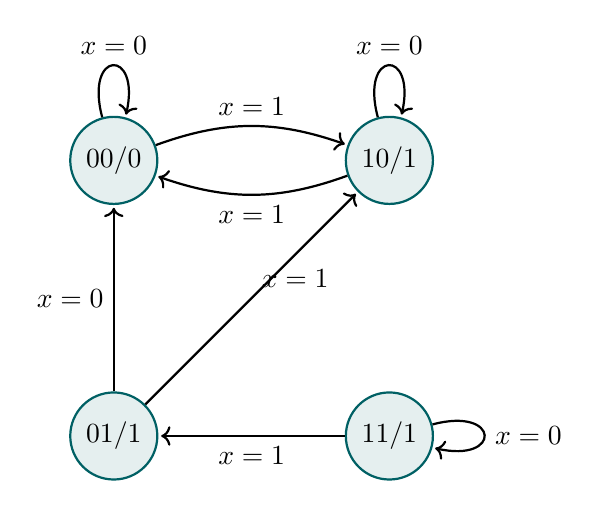
\begin{tikzpicture}[shorten >=1pt, node distance=3.5cm, on grid, auto, thick,
                    every state/.style={fill=cF!10, draw=cF, thick, minimum size=1cm}]
    
    % Nodes (Format: State / Output)
    \node[state] (S00) {$00 / 0$};
    \node[state] (S10) [right=of S00] {$10 / 1$};
    \node[state] (S01) [below=of S00] {$01 / 1$};
    \node[state] (S11) [right=of S01] {$11 / 1$};

    % Edges
    \path[->]
    (S00) edge [loop above] node {$x=0$} (S00)
          edge [bend left=20] node {$x=1$} (S10)
    
    (S10) edge [loop above] node {$x=0$} (S10)
          edge [bend left=20] node {$x=1$} (S00)
          
    (S01) edge node[left] {$x=0$} (S00)
          edge node[above right] {$x=1$} (S10)
          
    (S11) edge [loop right] node {$x=0$} (S11)
          edge node[below] {$x=1$} (S01);
          
\end{tikzpicture}
\end{center}

\end{tcolorbox}

\item A sequential circuit has two flip-flops $A$ and $B$, two inputs $x_1$ and $x_2$, and one output $z$. The flip-flop input equations and circuit output equations are:
\begin{align*}
  J_A &= y_A x_1 + y_B x_2,\quad  & K_A &= y_A y_B + x_1 x_2 \\
  J_B &= y_A x_1,\quad             & K_B &= y_A y_B x_1 + y_B x_2 \\
  z   &= y_A x_1 x_2 + y_B x_1 x_2
\end{align*}
\begin{enumerate}
  \item Draw the logic diagram of the circuit.
  \item Derive the transition table, excitation table and state table.
  \item Draw the state diagram.
\end{enumerate}
\mk{20} \yr{CSE 205 | L-2/T-1 | 2021--22}

\begin{tcolorbox}[enhanced,breakable,ansbox,colback=cF!4,colframe=cF,boxrule=0.8pt,arc=5pt,title={\textbf{Answer}},fonttitle=\bfseries\color{white},colbacktitle=cF]

\subsection*{(a) Logic Diagram Structural Description}
Given the structural complexity and density of feedback connections for this multi-input Mealy machine, a highly descriptive structural blueprint is provided to ensure error-free layout realization:

\begin{enumerate}
    \item \textbf{Memory Elements:} Two edge-triggered JK flip-flops labeled \textbf{Flip-Flop A} (generating state variable $y_A$ and complement $y_A'$) and \textbf{Flip-Flop B} (generating state variable $y_B$ and complement $y_B'$), driven by a shared common clock line (\text{CLK}).
    \item \textbf{Excitation Network for Flip-Flop A:}
    \begin{itemize}
        \item \textbf{$J_A$ Logic:} A 2-input AND gate computes $y_A x_1$, and another 2-input AND gate computes $y_B x_2$. The outputs of both gates feed into a 2-input OR gate connected directly to the $J_A$ terminal.
        \item \textbf{$K_A$ Logic:} A 2-input AND gate computes $y_A y_B$, and another 2-input AND gate computes $x_1 x_2$. The outputs feed into a 2-input OR gate connected to the $K_A$ terminal.
    \end{itemize}
    \item \textbf{Excitation Network for Flip-Flop B:}
    \begin{itemize}
        \item \textbf{$J_B$ Logic:} A single 2-input AND gate computes $y_A x_1$ and connects to the $J_B$ terminal.
        \item \textbf{$K_B$ Logic:} A 3-input AND gate computes $y_A y_B x_1$, and a 2-input AND gate computes $y_B x_2$. Their outputs feed into a 2-input OR gate connected to the $K_B$ terminal.
    \end{itemize}
    \item \textbf{Output Network ($z$):}
    \begin{itemize}
        \item A 3-input AND gate computes $y_A x_1 x_2$, and a second 3-input AND gate computes $y_B x_1 x_2$. Their outputs feed into a final 2-input OR gate to produce the Mealy output $z$.
    \end{itemize}
\end{enumerate}

\subsection*{(b) Derivation of Tables}

\textbf{1. Next-State Equations (Mathematical Derivations)}\\
The general characteristic equation for a JK flip-flop is given by $Q(t+1) = J \cdot Q' + K' \cdot Q$. We substitute the excitation equations into this template for both flip-flops.

For \textbf{Flip-Flop A}:
\begin{align*}
y_A(t+1) &= J_A y_A' + K_A' y_A \\
&= (y_A x_1 + y_B x_2) y_A' + (y_A y_B + x_1 x_2)' y_A \\
&= y_A y_A' x_1 + y_A' y_B x_2 + (y_A y_B)' (x_1 x_2)' y_A \quad && \text{(Distributive \& De Morgan's Laws)} \\
&= 0 + y_A' y_B x_2 + (y_A' + y_B')(x_1' + x_2') y_A \quad && \text{(Complementarity \& De Morgan's Laws)} \\
&= y_A' y_B x_2 + (y_A y_A' + y_A y_B')(x_1' + x_2') \quad && \text{(Distributive Law)} \\
&= y_A' y_B x_2 + (0 + y_A y_B')(x_1' + x_2') \quad && \text{(Complementarity Law)} \\
&= y_A' y_B x_2 + y_A y_B' x_1' + y_A y_B' x_2' \quad && \text{(Identity \& Distributive Laws)}
\end{align*}

For \textbf{Flip-Flop B}:
\begin{align*}
y_B(t+1) &= J_B y_B' + K_B' y_B \\
&= (y_A x_1) y_B' + (y_A y_B x_1 + y_B x_2)' y_B \\
&= y_A y_B' x_1 + [y_B (y_A x_1 + x_2)]' y_B \quad && \text{(Distributive Law)} \\
&= y_A y_B' x_1 + [y_B' + (y_A x_1 + x_2)'] y_B \quad && \text{(De Morgan's Law)} \\
&= y_A y_B' x_1 + y_B' y_B + (y_A x_1 + x_2)' y_B \quad && \text{(Distributive Law)} \\
&= y_A y_B' x_1 + 0 + (y_A x_1)' x_2' y_B \quad && \text{(Complementarity \& De Morgan's Laws)} \\
&= y_A y_B' x_1 + (y_A' + x_1') x_2' y_B \quad && \text{(De Morgan's Law)} \\
&= y_A y_B' x_1 + y_A' y_B x_2' + y_B x_1' x_2' \quad && \text{(Distributive Law)}
\end{align*}

\newpage
\textbf{2. Excitation and Transition Table}\\
By systematically substituting all $2^4 = 16$ combinations of state ($y_A y_B$) and inputs ($x_1 x_2$), we compile the detailed excitation and transition data.

\begin{center}
\renewcommand{\arraystretch}{1.2}
\small
\begin{tabular}{cccc|cccc|cc|c}
\toprule
\multicolumn{2}{c}{\textbf{Present State}} & \multicolumn{2}{c|}{\textbf{Inputs}} & \multicolumn{4}{c|}{\textbf{Excitation Inputs}} & \multicolumn{2}{c|}{\textbf{Next State}} & \textbf{Output} \\
$y_A$ & $y_B$ & $x_1$ & $x_2$ & $J_A$ & $K_A$ & $J_B$ & $K_B$ & $y_A(t+1)$ & $y_B(t+1)$ & $z$ \\
\midrule
0 & 0 & 0 & 0 & 0 & 0 & 0 & 0 & 0 & 0 & 0 \\
0 & 0 & 0 & 1 & 0 & 0 & 0 & 0 & 0 & 0 & 0 \\
0 & 0 & 1 & 0 & 0 & 0 & 0 & 0 & 0 & 0 & 0 \\
0 & 0 & 1 & 1 & 0 & 1 & 0 & 0 & 0 & 0 & 0 \\
\midrule
0 & 1 & 0 & 0 & 0 & 0 & 0 & 0 & 0 & 1 & 0 \\
0 & 1 & 0 & 1 & 1 & 0 & 0 & 1 & 1 & 0 & 0 \\
0 & 1 & 1 & 0 & 0 & 0 & 0 & 0 & 0 & 1 & 0 \\
0 & 1 & 1 & 1 & 1 & 1 & 0 & 1 & 1 & 0 & 1 \\
\midrule
1 & 0 & 0 & 0 & 0 & 0 & 0 & 0 & 1 & 0 & 0 \\
1 & 0 & 0 & 1 & 0 & 0 & 0 & 0 & 1 & 0 & 0 \\
1 & 0 & 1 & 0 & 1 & 0 & 1 & 0 & 1 & 1 & 0 \\
1 & 0 & 1 & 1 & 1 & 1 & 1 & 0 & 0 & 1 & 1 \\
\midrule
1 & 1 & 0 & 0 & 0 & 1 & 0 & 0 & 0 & 1 & 0 \\
1 & 1 & 0 & 1 & 1 & 1 & 0 & 1 & 0 & 0 & 0 \\
1 & 1 & 1 & 0 & 1 & 1 & 1 & 0 & 0 & 0 & 0 \\
1 & 1 & 1 & 1 & 1 & 1 & 1 & 1 & 0 & 0 & 1 \\
\bottomrule
\end{tabular}
\end{center}

\vspace{1em}
\textbf{3. Compact State Table}\\
Consolidating the data into a standard state table showing the mapping from present state to next state and output under all input variations:

\begin{center}
\renewcommand{\arraystretch}{1.3}
\begin{tabular}{c|cccc|cccc}
\toprule
\textbf{Present State} & \multicolumn{4}{c|}{\textbf{Next State $y_A(t+1) y_B(t+1)$}} & \multicolumn{4}{c}{\textbf{Output $z$}} \\
$y_A y_B$ & $x_1 x_2 = 00$ & $01$ & $10$ & $11$ & $x_1 x_2 = 00$ & $01$ & $10$ & $11$ \\
\midrule
00 & 00 & 00 & 00 & 00 & 0 & 0 & 0 & 0 \\
01 & 01 & 10 & 01 & 10 & 0 & 0 & 0 & 1 \\
10 & 10 & 10 & 11 & 01 & 0 & 0 & 0 & 1 \\
11 & 01 & 00 & 00 & 00 & 0 & 0 & 0 & 1 \\
\bottomrule
\end{tabular}
\end{center}

\vspace{1em}
\subsection*{(c) State Diagram}
Below is the complete Mealy finite state machine representation. Arc transitions are formatted as $\text{Inputs } (x_1 x_2) / \text{Output } (z)$.

\begin{center}
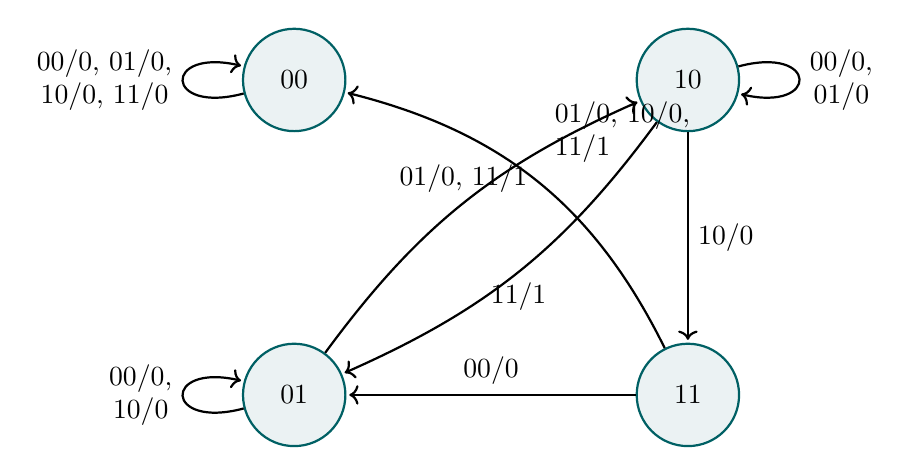
\begin{tikzpicture}[shorten >=1pt, node distance=4.5cm, on grid, auto, thick,
                    every state/.style={fill=cF!8, draw=cF, thick, minimum size=1.3cm}]
    
    % Node Placements
    \node[state] (S00) at (0,4)  {$00$};
    \node[state] (S01) at (0,0)  {$01$};
    \node[state] (S10) at (5,4)  {$10$};
    \node[state] (S11) at (5,0)  {$11$};

    % Graph Path Operations
    \path[->]
    (S00) edge [loop left] node [align=center] {00/0, 01/0,\\10/0, 11/0} (S00)
    
    (S01) edge [loop left] node [align=center] {00/0,\\10/0} (S01)
          edge [bend left=15] node [above] {01/0, 11/1} (S10)
          
    (S10) edge [loop right] node [align=center] {00/0,\\01/0} (S10)
          edge [bend left=15] node [below] {11/1} (S01)
          edge node [right] {10/0} (S11)
          
    (S11) edge node [above] {00/0} (S01)
          edge [bend right=25] node [above right=0.1cm and 0.1cm, align=left] {01/0, 10/0,\\11/1} (S00);
\end{tikzpicture}
\end{center}

\end{tcolorbox}

%% -- Q7(b): Analyze sequential circuit; transition, excitation, state table (figure-based) --
\item A sequential circuit has two flip-flops $A$ and $B$, two inputs $x_1$ and $x_2$, and one output $z$. The flip-flop input equations and circuit output equations are:
\begin{align*}
  J_A &= y_A x_1 + y_B x_2,\quad  & K_A &= y_A y_B + x_1 x_2 \\
  J_B &= y_A x_1,\quad             & K_B &= y_A y_B x_1 + y_B x_2 \\
  z   &= y_A x_1 x_2 + y_B x_1 x_2
\end{align*}

For the above circuit:
\begin{enumerate}
  \item Draw the logic diagram of the circuit.
  \item Derive the transition table, excitation table, and state table.
  \item Draw the state diagram.
\end{enumerate}
\mk{25} \yr{CSE 205 | L-2/T-1 | 2019--20}

\begin{tcolorbox}[enhanced,breakable,ansbox,colback=cF!4,colframe=cF,boxrule=0.8pt,arc=5pt,title={\textbf{Answer}},fonttitle=\bfseries\color{white},colbacktitle=cF]

\subsection*{(a) Logic Diagram Structural Description}
Given the structural complexity and density of feedback connections for this multi-input Mealy machine, a highly descriptive structural blueprint is provided to ensure an error-free layout realization (as drawing it with standard wire routing would result in excessive overlapping lines):

\begin{enumerate}
    \item \textbf{Memory Elements:} Two edge-triggered JK flip-flops designated as \textbf{FF A} (producing state variables $y_A, y_A'$) and \textbf{FF B} (producing state variables $y_B, y_B'$), synchronized by a common clock signal (\text{CLK}).
    \item \textbf{Combinational Excitation Network for FF A:}
    \begin{itemize}
        \item \textbf{$J_A$ Logic:} A 2-input AND gate computes $y_A x_1$, and another 2-input AND gate computes $y_B x_2$. Their outputs feed into a 2-input OR gate driving the $J_A$ terminal.
        \item \textbf{$K_A$ Logic:} A 2-input AND gate computes $y_A y_B$, and another 2-input AND gate computes $x_1 x_2$. Their outputs feed into a 2-input OR gate driving the $K_A$ terminal.
    \end{itemize}
    \item \textbf{Combinational Excitation Network for FF B:}
    \begin{itemize}
        \item \textbf{$J_B$ Logic:} A single 2-input AND gate computes $y_A x_1$ and connects directly to the $J_B$ terminal.
        \item \textbf{$K_B$ Logic:} A 3-input AND gate computes $y_A y_B x_1$, and a 2-input AND gate computes $y_B x_2$. Their outputs feed into a 2-input OR gate driving the $K_B$ terminal.
    \end{itemize}
    \item \textbf{Output Network ($z$):}
    \begin{itemize}
        \item A 3-input AND gate computes $y_A x_1 x_2$, and a second 3-input AND gate computes $y_B x_1 x_2$. Their outputs feed into a 2-input OR gate to generate the Mealy output $z$. Alternatively, this can be simplified to a 3-input AND gate computing $(y_A + y_B) x_1 x_2$.
    \end{itemize}
\end{enumerate}

\vspace{1em}
\subsection*{(b) Derivation of Tables}

\textbf{1. Next-State Equations (Mathematical Derivations)}\\
The characteristic equation for a JK flip-flop is $Q(t+1) = J \cdot Q' + K' \cdot Q$. We substitute the provided excitation equations into this formula for both flip-flops.

\noindent For \textbf{Flip-Flop A}:
\begin{align*}
y_A(t+1) &= J_A y_A' + K_A' y_A \\
&= (y_A x_1 + y_B x_2) y_A' + (y_A y_B + x_1 x_2)' y_A \\
&= y_A y_A' x_1 + y_A' y_B x_2 + (y_A y_B)' (x_1 x_2)' y_A \quad && \text{(Distributive \& De Morgan's Laws)} \\
&= 0 + y_A' y_B x_2 + (y_A' + y_B')(x_1' + x_2') y_A \quad && \text{(Complementarity \& De Morgan's Laws)} \\
&= y_A' y_B x_2 + (y_A y_A' + y_A y_B')(x_1' + x_2') \quad && \text{(Distributive Law)} \\
&= y_A' y_B x_2 + (0 + y_A y_B')(x_1' + x_2') \quad && \text{(Complementarity Law)} \\
&= y_A' y_B x_2 + y_A y_B' x_1' + y_A y_B' x_2' \quad && \text{(Identity \& Distributive Laws)}
\end{align*}

\noindent For \textbf{Flip-Flop B}:
\begin{align*}
y_B(t+1) &= J_B y_B' + K_B' y_B \\
&= (y_A x_1) y_B' + (y_A y_B x_1 + y_B x_2)' y_B \\
&= y_A y_B' x_1 + [y_B (y_A x_1 + x_2)]' y_B \quad && \text{(Distributive Law)} \\
&= y_A y_B' x_1 + [y_B' + (y_A x_1 + x_2)'] y_B \quad && \text{(De Morgan's Law)} \\
&= y_A y_B' x_1 + y_B' y_B + (y_A x_1 + x_2)' y_B \quad && \text{(Distributive Law)} \\
&= y_A y_B' x_1 + 0 + (y_A x_1)' x_2' y_B \quad && \text{(Complementarity \& De Morgan's Laws)} \\
&= y_A y_B' x_1 + (y_A' + x_1') x_2' y_B \quad && \text{(De Morgan's Law)} \\
&= y_A y_B' x_1 + y_A' y_B x_2' + y_B x_1' x_2' \quad && \text{(Distributive Law)}
\end{align*}

\newpage
\textbf{2. Excitation and Transition Table}\\
Evaluating the excitation formulas and the derived next-state equations for all $2^4 = 16$ permutations of states ($y_A, y_B$) and inputs ($x_1, x_2$), we compile the comprehensive transition table. The output is simplified as $z = (y_A + y_B)x_1 x_2$.

\begin{center}
\renewcommand{\arraystretch}{1.2}
\small
\begin{tabular}{cccc|cccc|cc|c}
\toprule
\multicolumn{2}{c}{\textbf{Present State}} & \multicolumn{2}{c|}{\textbf{Inputs}} & \multicolumn{4}{c|}{\textbf{Excitation Inputs}} & \multicolumn{2}{c|}{\textbf{Next State}} & \textbf{Output} \\
$y_A$ & $y_B$ & $x_1$ & $x_2$ & $J_A$ & $K_A$ & $J_B$ & $K_B$ & $y_A(t+1)$ & $y_B(t+1)$ & $z$ \\
\midrule
0 & 0 & 0 & 0 & 0 & 0 & 0 & 0 & 0 & 0 & 0 \\
0 & 0 & 0 & 1 & 0 & 0 & 0 & 0 & 0 & 0 & 0 \\
0 & 0 & 1 & 0 & 0 & 0 & 0 & 0 & 0 & 0 & 0 \\
0 & 0 & 1 & 1 & 0 & 1 & 0 & 0 & 0 & 0 & 0 \\
\midrule
0 & 1 & 0 & 0 & 0 & 0 & 0 & 0 & 0 & 1 & 0 \\
0 & 1 & 0 & 1 & 1 & 0 & 0 & 1 & 1 & 0 & 0 \\
0 & 1 & 1 & 0 & 0 & 0 & 0 & 0 & 0 & 1 & 0 \\
0 & 1 & 1 & 1 & 1 & 1 & 0 & 1 & 1 & 0 & 1 \\
\midrule
1 & 0 & 0 & 0 & 0 & 0 & 0 & 0 & 1 & 0 & 0 \\
1 & 0 & 0 & 1 & 0 & 0 & 0 & 0 & 1 & 0 & 0 \\
1 & 0 & 1 & 0 & 1 & 0 & 1 & 0 & 1 & 1 & 0 \\
1 & 0 & 1 & 1 & 1 & 1 & 1 & 0 & 0 & 1 & 1 \\
\midrule
1 & 1 & 0 & 0 & 0 & 1 & 0 & 0 & 0 & 1 & 0 \\
1 & 1 & 0 & 1 & 1 & 1 & 0 & 1 & 0 & 0 & 0 \\
1 & 1 & 1 & 0 & 1 & 1 & 1 & 0 & 0 & 0 & 0 \\
1 & 1 & 1 & 1 & 1 & 1 & 1 & 1 & 0 & 0 & 1 \\
\bottomrule
\end{tabular}
\end{center}

\vspace{1em}
\textbf{3. Compact State Table}\\
By grouping the next state and output combinations based on input pairs ($x_1 x_2$), we format the traditional state table:

\begin{center}
\renewcommand{\arraystretch}{1.3}
\begin{tabular}{c|cccc|cccc}
\toprule
\textbf{Present State} & \multicolumn{4}{c|}{\textbf{Next State $y_A(t+1) y_B(t+1)$}} & \multicolumn{4}{c}{\textbf{Output $z$}} \\
$y_A y_B$ & $x_1 x_2 = 00$ & $01$ & $10$ & $11$ & $x_1 x_2 = 00$ & $01$ & $10$ & $11$ \\
\midrule
00 & 00 & 00 & 00 & 00 & 0 & 0 & 0 & 0 \\
01 & 01 & 10 & 01 & 10 & 0 & 0 & 0 & 1 \\
10 & 10 & 10 & 11 & 01 & 0 & 0 & 0 & 1 \\
11 & 01 & 00 & 00 & 00 & 0 & 0 & 0 & 1 \\
\bottomrule
\end{tabular}
\end{center}

\vspace{1em}
\subsection*{(c) State Diagram}
The directed graph below illustrates the state transitions. Edges are labeled as $\text{Inputs } (x_1 x_2) \, / \, \text{Output } (z)$. Since multiple input conditions can trigger the same transition, they are grouped to preserve clarity.

\begin{center}
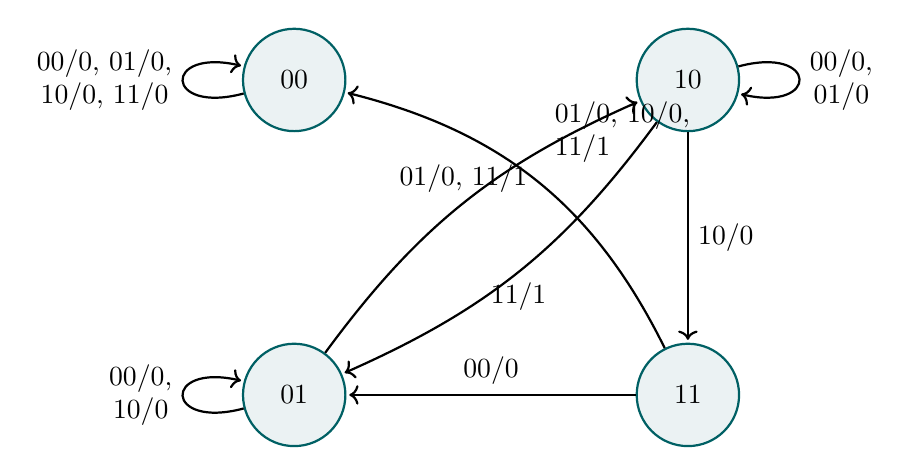
\begin{tikzpicture}[shorten >=1pt, node distance=4.5cm, on grid, auto, thick,
                    every state/.style={fill=cF!8, draw=cF, thick, minimum size=1.3cm}]
    
    % Node Placements
    \node[state] (S00) at (0,4)  {$00$};
    \node[state] (S01) at (0,0)  {$01$};
    \node[state] (S10) at (5,4)  {$10$};
    \node[state] (S11) at (5,0)  {$11$};

    % Graph Path Operations
    \path[->]
    (S00) edge [loop left] node [align=center] {00/0, 01/0,\\10/0, 11/0} (S00)
    
    (S01) edge [loop left] node [align=center] {00/0,\\10/0} (S01)
          edge [bend left=15] node [above] {01/0, 11/1} (S10)
          
    (S10) edge [loop right] node [align=center] {00/0,\\01/0} (S10)
          edge [bend left=15] node [below] {11/1} (S01)
          edge node [right] {10/0} (S11)
          
    (S11) edge node [above] {00/0} (S01)
          edge [bend right=25] node [above right=0.1cm and 0.1cm, align=left] {01/0, 10/0,\\11/1} (S00);
\end{tikzpicture}
\end{center}

\end{tcolorbox}

\item A sequential circuit has two JK Flip-Flops $A$ and $B$, two inputs $x$ and $y$, and one output $z$. The flip-flop input equations and circuit output equation are:
\begin{align*}
  J_A &= Ax + By,\quad & K_A &= AB + xy \\
  J_B &= Ax,\quad & K_B &= ABx + By,\quad & z &= Axy + Bxy
\end{align*}
\begin{enumerate}
  \item Draw the logic diagram of the circuit.
  \item Derive the state table.
  \item Draw the state diagram.
  \end{enumerate}
\mk{4+7+4} \yr{CSE 205 | L-2/T-1 | 2016--17}

\begin{tcolorbox}[enhanced,breakable,ansbox,colback=cF!4,colframe=cF,boxrule=0.8pt,arc=5pt,title={\textbf{Answer}},fonttitle=\bfseries\color{white},colbacktitle=cF]

\subsection*{(a) Logic Diagram Structural Description}
Given the structural complexity and density of feedback connections for this multi-input Mealy machine, a highly descriptive structural blueprint is provided to ensure an error-free layout realization (as drawing it with standard wire routing would result in excessive overlapping lines):

\begin{enumerate}
    \item \textbf{Memory Elements:} Two edge-triggered JK flip-flops designated as \textbf{FF A} (producing state variables $A, A'$) and \textbf{FF B} (producing state variables $B, B'$), synchronized by a common clock signal (\text{CLK}).
    \item \textbf{Combinational Excitation Network for FF A:}
    \begin{itemize}
        \item \textbf{$J_A$ Logic:} A 2-input AND gate computes $Ax$, and another 2-input AND gate computes $By$. Their outputs feed into a 2-input OR gate driving the $J_A$ terminal.
        \item \textbf{$K_A$ Logic:} A 2-input AND gate computes $AB$, and another 2-input AND gate computes $xy$. Their outputs feed into a 2-input OR gate driving the $K_A$ terminal.
    \end{itemize}
    \item \textbf{Combinational Excitation Network for FF B:}
    \begin{itemize}
        \item \textbf{$J_B$ Logic:} A single 2-input AND gate computes $Ax$ and connects directly to the $J_B$ terminal.
        \item \textbf{$K_B$ Logic:} A 3-input AND gate computes $ABx$, and a 2-input AND gate computes $By$. Their outputs feed into a 2-input OR gate driving the $K_B$ terminal.
    \end{itemize}
    \item \textbf{Output Network ($z$):}
    \begin{itemize}
        \item The output is defined as $z = Axy + Bxy$. A simplified implementation uses a 2-input OR gate to compute $(A + B)$, which then feeds into a 3-input AND gate alongside inputs $x$ and $y$ to generate the Mealy output $z$.
    \end{itemize}
\end{enumerate}

\vspace{1em}
\subsection*{(b) Derivation of the State Table}

\textbf{1. Next-State Equations (Mathematical Derivations)}\\
The characteristic equation for a JK flip-flop is $Q(t+1) = J \cdot Q' + K' \cdot Q$. We substitute the provided excitation equations into this formula for both flip-flops.

\noindent For \textbf{Flip-Flop A}:
\begin{align*}
A(t+1) &= J_A A' + K_A' A \\
&= (Ax + By) A' + (AB + xy)' A \\
&= A A' x + A' B y + ( (AB)' (xy)' ) A \quad && \text{(Distributive \& De Morgan's Laws)} \\
&= 0 + A' B y + ( (A' + B')(x' + y') ) A \quad && \text{(Complementarity \& De Morgan's Laws)} \\
&= A' B y + (A A' + A B')(x' + y') \quad && \text{(Distributive Law)} \\
&= A' B y + (0 + A B')(x' + y') \quad && \text{(Complementarity Law)} \\
&= A' B y + A B' x' + A B' y' \quad && \text{(Identity \& Distributive Laws)}
\end{align*}

\noindent For \textbf{Flip-Flop B}:
\begin{align*}
B(t+1) &= J_B B' + K_B' B \\
&= (Ax) B' + (ABx + By)' B \\
&= A B' x + ( (ABx)' (By)' ) B \quad && \text{(Distributive \& De Morgan's Laws)} \\
&= A B' x + ( (A' + B' + x')(B' + y') ) B \quad && \text{(De Morgan's Law)} \\
&= A B' x + (A' + B' + x')(B B' + B y') \quad && \text{(Distributive Law)} \\
&= A B' x + (A' + B' + x')(0 + B y') \quad && \text{(Complementarity Law)} \\
&= A B' x + A' B y' + B B' y' + B x' y' \quad && \text{(Distributive Law)} \\
&= A B' x + A' B y' + B x' y' \quad && \text{(Complementarity Law)}
\end{align*}

\newpage
\textbf{2. Excitation and Transition Table}\\
Evaluating the excitation formulas and the derived next-state equations for all $2^4 = 16$ permutations of states ($A, B$) and inputs ($x, y$), we compile the comprehensive transition table. 

\begin{center}
\renewcommand{\arraystretch}{1.2}
\small
\begin{tabular}{cccc|cccc|cc|c}
\toprule
\multicolumn{2}{c}{\textbf{Present State}} & \multicolumn{2}{c|}{\textbf{Inputs}} & \multicolumn{4}{c|}{\textbf{Excitation Inputs}} & \multicolumn{2}{c|}{\textbf{Next State}} & \textbf{Output} \\
$A$ & $B$ & $x$ & $y$ & $J_A$ & $K_A$ & $J_B$ & $K_B$ & $A(t+1)$ & $B(t+1)$ & $z$ \\
\midrule
0 & 0 & 0 & 0 & 0 & 0 & 0 & 0 & 0 & 0 & 0 \\
0 & 0 & 0 & 1 & 0 & 0 & 0 & 0 & 0 & 0 & 0 \\
0 & 0 & 1 & 0 & 0 & 0 & 0 & 0 & 0 & 0 & 0 \\
0 & 0 & 1 & 1 & 0 & 1 & 0 & 0 & 0 & 0 & 0 \\
\midrule
0 & 1 & 0 & 0 & 0 & 0 & 0 & 0 & 0 & 1 & 0 \\
0 & 1 & 0 & 1 & 1 & 0 & 0 & 1 & 1 & 0 & 0 \\
0 & 1 & 1 & 0 & 0 & 0 & 0 & 0 & 0 & 1 & 0 \\
0 & 1 & 1 & 1 & 1 & 1 & 0 & 1 & 1 & 0 & 1 \\
\midrule
1 & 0 & 0 & 0 & 0 & 0 & 0 & 0 & 1 & 0 & 0 \\
1 & 0 & 0 & 1 & 0 & 0 & 0 & 0 & 1 & 0 & 0 \\
1 & 0 & 1 & 0 & 1 & 0 & 1 & 0 & 1 & 1 & 0 \\
1 & 0 & 1 & 1 & 1 & 1 & 1 & 0 & 0 & 1 & 1 \\
\midrule
1 & 1 & 0 & 0 & 0 & 1 & 0 & 0 & 0 & 1 & 0 \\
1 & 1 & 0 & 1 & 1 & 1 & 0 & 1 & 0 & 0 & 0 \\
1 & 1 & 1 & 0 & 1 & 1 & 1 & 0 & 0 & 0 & 0 \\
1 & 1 & 1 & 1 & 1 & 1 & 1 & 1 & 0 & 0 & 1 \\
\bottomrule
\end{tabular}
\end{center}

\vspace{1em}
\textbf{3. Compact State Table}\\
Consolidating the data into a standard two-dimensional state table showing the transitions and outputs:

\begin{center}
\renewcommand{\arraystretch}{1.3}
\begin{tabular}{c|cccc|cccc}
\toprule
\textbf{Present State} & \multicolumn{4}{c|}{\textbf{Next State $A(t+1) B(t+1)$}} & \multicolumn{4}{c}{\textbf{Output $z$}} \\
$AB$ & $xy = 00$ & $01$ & $10$ & $11$ & $xy = 00$ & $01$ & $10$ & $11$ \\
\midrule
00 & 00 & 00 & 00 & 00 & 0 & 0 & 0 & 0 \\
01 & 01 & 10 & 01 & 10 & 0 & 0 & 0 & 1 \\
10 & 10 & 10 & 11 & 01 & 0 & 0 & 0 & 1 \\
11 & 01 & 00 & 00 & 00 & 0 & 0 & 0 & 1 \\
\bottomrule
\end{tabular}
\end{center}

\vspace{1em}
\subsection*{(c) State Diagram}
The directed graph below illustrates the state transitions. Edges are labeled as $\text{Inputs } (xy) \, / \, \text{Output } (z)$. To prevent visual clutter, transitions spanning multiple input conditions between the same nodes are grouped together.

\begin{center}
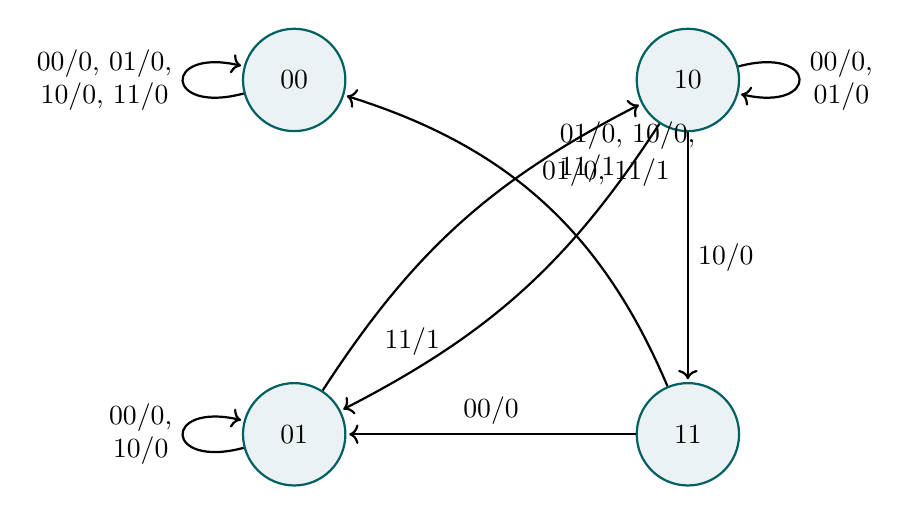
\begin{tikzpicture}[shorten >=1pt, node distance=4.5cm, on grid, auto, thick,
                    every state/.style={fill=cF!8, draw=cF, thick, minimum size=1.3cm}]
    
    % Node Placements
    \node[state] (S00) at (0,4.5)  {$00$};
    \node[state] (S01) at (0,0)    {$01$};
    \node[state] (S10) at (5,4.5)  {$10$};
    \node[state] (S11) at (5,0)    {$11$};

    % Graph Path Operations
    \path[->]
    (S00) edge [loop left] node [align=center] {00/0, 01/0,\\10/0, 11/0} (S00)
    
    (S01) edge [loop left] node [align=center] {00/0,\\10/0} (S01)
          edge [bend left=15] node [pos=0.7, right=0.1cm] {01/0, 11/1} (S10)
          
    (S10) edge [loop right] node [align=center] {00/0,\\01/0} (S10)
          edge [bend left=15] node [pos=0.7, left=0.1cm] {11/1} (S01)
          edge node [right] {10/0} (S11)
          
    (S11) edge node [above] {00/0} (S01)
          edge [bend right=25] node [above right=0.1cm and 0.1cm, align=left] {01/0, 10/0,\\11/1} (S00);
\end{tikzpicture}
\end{center}

\end{tcolorbox}

\item A sequential circuit has two JK Flip-Flops $A$ and $B$, two inputs $x$ and $y$, and one output $z$. The Flip-Flop input equations and circuit output equation are:
\[
  J_A = Bx + B'y',\quad K_A = B'xy',\quad J_B = A'x,\quad K_B = A + xy',\quad z = Ax'y' + Bx'y'
\]
Draw the logic diagram of the circuit, tabulate the state table and derive the state equations for $A$ and $B$.
\mk{15} \yr{CSE 205 | L-2/T-1 | 2014--15}

\begin{tcolorbox}[enhanced,breakable,ansbox,colback=cF!4,colframe=cF,boxrule=0.8pt,arc=5pt,title={\textbf{Answer}},fonttitle=\bfseries\color{white},colbacktitle=cF]

\subsection*{(a) Logic Diagram Structural Description}
Given the structural complexity and density of feedback connections for this multi-input Mealy machine, a highly descriptive structural blueprint is provided to ensure an error-free layout realization:

\begin{enumerate}
    \item \textbf{Memory Elements:} Two edge-triggered JK flip-flops designated as \textbf{FF A} (producing state variables $A, A'$) and \textbf{FF B} (producing state variables $B, B'$), synchronized by a common clock signal (\text{CLK}).
    \item \textbf{Combinational Excitation Network for FF A:}
    \begin{itemize}
        \item \textbf{$J_A$ Logic:} A 2-input AND gate computes $Bx$, and another 2-input AND gate computes $B'y'$. Their outputs feed into a 2-input OR gate driving the $J_A$ terminal.
        \item \textbf{$K_A$ Logic:} A 3-input AND gate computes $B'xy'$ and connects directly to the $K_A$ terminal.
    \end{itemize}
    \item \textbf{Combinational Excitation Network for FF B:}
    \begin{itemize}
        \item \textbf{$J_B$ Logic:} A 2-input AND gate computes $A'x$ and connects directly to the $J_B$ terminal.
        \item \textbf{$K_B$ Logic:} A 2-input AND gate computes $xy'$. Its output feeds into a 2-input OR gate alongside signal $A$, driving the $K_B$ terminal.
    \end{itemize}
    \item \textbf{Output Network ($z$):}
    \begin{itemize}
        \item The output is defined as $z = Ax'y' + Bx'y'$. This can be structurally implemented using a 3-input AND gate for $Ax'y'$, another 3-input AND gate for $Bx'y'$, and a 2-input OR gate to sum them. (Alternatively, a simplified structure uses an OR gate for $(A+B)$ feeding into a 3-input AND gate with $x'$ and $y'$).
    \end{itemize}
\end{enumerate}

\vspace{1em}
\subsection*{(b) Derivation of the State Equations}

The characteristic equation for a JK flip-flop is defined as $Q(t+1) = J \cdot Q' + K' \cdot Q$. We derive the next-state equations by substituting the provided excitation equations into this characteristic formula.

\noindent \textbf{State Equation for Flip-Flop A:}
\begin{align*}
A(t+1) &= J_A A' + K_A' A \\
&= (Bx + B'y') A' + (B'xy')' A \\
&= A'Bx + A'B'y' + (B + (xy')') A \quad && \text{(Distributive \& De Morgan's Laws)} \\
&= A'Bx + A'B'y' + (B + x' + y) A \quad && \text{(De Morgan's Law)} \\
&= A'Bx + A'B'y' + AB + Ax' + Ay \quad && \text{(Distributive Law)}
\end{align*}

\noindent \textbf{State Equation for Flip-Flop B:}
\begin{align*}
B(t+1) &= J_B B' + K_B' B \\
&= (A'x) B' + (A + xy')' B \\
&= A'B'x + ( A' \cdot (xy')' ) B \quad && \text{(Distributive \& De Morgan's Laws)} \\
&= A'B'x + A' (x' + y) B \quad && \text{(De Morgan's Law)} \\
&= A'B'x + A'Bx' + A'By \quad && \text{(Distributive Law)}
\end{align*}

\vspace{1em}
\subsection*{(c) State Table}

By evaluating the derived state equations $A(t+1)$ and $B(t+1)$, alongside the output equation $z = Ax'y' + Bx'y'$, for all $2^4 = 16$ permutations of present states ($A, B$) and inputs ($x, y$), we construct the comprehensive state table.

\textbf{Compact State Table Representation:}
\begin{center}
\renewcommand{\arraystretch}{1.3}
\begin{tabular}{c|cccc|cccc}
\toprule
\textbf{Present State} & \multicolumn{4}{c|}{\textbf{Next State $A(t+1) B(t+1)$}} & \multicolumn{4}{c}{\textbf{Output $z$}} \\
$AB$ & $xy = 00$ & $01$ & $10$ & $11$ & $xy = 00$ & $01$ & $10$ & $11$ \\
\midrule
00 & 10 & 00 & 11 & 01 & 0 & 0 & 0 & 0 \\
01 & 01 & 01 & 10 & 11 & 1 & 0 & 0 & 0 \\
10 & 10 & 10 & 00 & 10 & 1 & 0 & 0 & 0 \\
11 & 10 & 10 & 10 & 10 & 1 & 0 & 0 & 0 \\
\bottomrule
\end{tabular}
\end{center}

\vspace{1em}
\noindent \textit{Verification Note for Output:} The output equation $z = Ax'y' + Bx'y' = (A+B)x'y'$ asserts that $z = 1$ strictly when $x=0$, $y=0$, and the present state $AB$ is not $00$. This perfectly maps to the output partition of the state table above.

\end{tcolorbox}

\item Derive the state diagram from the following sequential circuit.

\begin{center}
\begin{circuitikz}[thick, scale=0.9, transform shape]
        
        % ----------------------------------------------------
        % Define components and their coordinates
        % ----------------------------------------------------
        \coordinate (x_in) at (0, 3);
        \node[not port] (not1) at (2.5, 3) {};
        \node[and port] (and1) at (4.5, 6.5) {};
        \node[or port]  (or1)  at (4.5, -0.5) {};
        \node[and port] (and2) at (10, 8) {};
        
        % ----------------------------------------------------
        % Top Flip-Flop (FF1)
        % ----------------------------------------------------
        \draw[thick] (6, 4) rectangle (8, 7);
        \node[right] at (6, 6.5) {$J_1$};
        \node[right] at (6, 4.5) {$K_1$};
        \node[right] at (6.2, 5.5) {$C$};
        \node[left]  at (8, 6.5) {$Q$};
        \node[left]  at (8, 4.5) {$\bar{Q}$};
        
        % Clock bubble and triangle for FF1
        \draw (5.8, 5.5) -- (5.9, 5.5);
        \draw (5.95, 5.5) circle(0.05); % bubble
        \draw (6, 5.35) -- (6.2, 5.5) -- (6, 5.65); % triangle
        
        % ----------------------------------------------------
        % Bottom Flip-Flop (FF2)
        % ----------------------------------------------------
        \draw[thick] (6, -1) rectangle (8, 2);
        \node[right] at (6, 1.5) {$J_2$};
        \node[right] at (6, -0.5) {$K_2$};
        \node[right] at (6.2, 0.5) {$C$};
        \node[left]  at (8, 1.5) {$Q$};
        \node[left]  at (8, -0.5) {$\bar{Q}$};
        
        % Clock bubble and triangle for FF2
        \draw (5.8, 0.5) -- (5.9, 0.5);
        \draw (5.95, 0.5) circle(0.05); % bubble
        \draw (6, 0.35) -- (6.2, 0.5) -- (6, 0.65); % triangle
        
        % ----------------------------------------------------
        % Wiring
        % ----------------------------------------------------
        
        % Input x wiring
        \draw (x_in) node[left] {$x$} -- (not1.in);
        \coordinate (x_tap_up) at (1, 3);
        \coordinate (x_tap_down) at (1.5, 3);
        
        \draw (x_tap_up) node[circ]{} |- (and1.in 1);
        \draw (x_tap_down) node[circ]{} |- (6, 1.5); % Connects to J2
        
        % NOT gate wiring (x')
        \coordinate (not_tap) at (3.5, 3);
        \draw (not1.out) -- (not_tap);
        \draw (not_tap) node[circ]{} |- (6, 4.5); % Connects to K1
        \draw (not_tap) node[circ]{} |-(3.5 , 2) |- (2.5, 2)  |- (or1.in 1); % Connects to OR1
        
        % AND1 output wiring
        \draw (and1.out) -- (6, 6.5); % Connects to J1
        \coordinate (and1_tap) at (5, 6.5);
        \draw (and1_tap) node[circ]{} |- (and2.in 1); % Connects to Output AND
        
        % OR1 output wiring
        \draw (or1.out) -- (6, -0.5); % Connects to K2
        
        % FF1 Output wiring (y1 and y1_bar)
        \draw (8, 6.5) -- (9, 6.5) node[right] {$y_1$};
        \coordinate (y1_tap) at (8.5, 6.5);
        \draw (y1_tap) node[circ]{} |- (and2.in 2);
        
        \draw (8, 4.5) -- (10, 4.5) node[right] {$\bar{y}_1$};
        \coordinate (y1bar_tap) at (10, 4.5);
        \draw (y1bar_tap) node[circ]{} |- (3, -2) |- (or1.in 2); % Feedback to OR1
        
        % FF2 Output wiring (y2 and y2_bar)
        \draw (8, 1.5) -- (9, 1.5) node[right] {$y_2$};
        \coordinate (y2_tap) at (9, 1.5);
        \draw (y2_tap) node[circ]{} |- (3, 3.5) |- (and1.in 2); % Feedback to Top AND1
        
        \draw (8, -0.5) -- (9, -0.5) node[right] {$\bar{y}_2$};
        
        % Final Output z wiring
        \draw (and2.out) -- (11, 8) node[right] {$z$};
        
        % Global Clock Line
        \draw (5.5, -2.5) node[below] {Clock} -- (5.5, 6);
        \draw (5.5, 5.5) node[circ]{} -- (5.8, 5.5);
        \draw (5.5, 0.5) node[circ]{} -- (5.8, 0.5);
        
    \end{circuitikz}
\end{center}
\mk{15} \yr{CSE 205 | L-2/T-1 | 2012--13}

\begin{tcolorbox}[enhanced,breakable,ansbox,colback=cF!4,colframe=cF,boxrule=0.8pt,arc=5pt,title={\textbf{Answer}},fonttitle=\bfseries\color{white},colbacktitle=cF]

\subsection*{1. Excitation and Output Equations}
By analyzing the provided logic diagram, we trace the logic gates connected to the JK flip-flop inputs and the circuit's final output. Let $y_1$ and $y_2$ represent the state variables for Flip-Flop 1 (FF1) and Flip-Flop 2 (FF2), respectively. 

\begin{itemize}
    \item \textbf{FF1 Inputs:} The $J_1$ input is driven by a 2-input AND gate receiving $x$ and $y_2$. The $K_1$ input is driven by a NOT gate connected to $x$.
    \[ J_1 = x y_2, \quad K_1 = x' \]
    
    \item \textbf{FF2 Inputs:} The $J_2$ input is directly connected to $x$. The $K_2$ input is driven by a 2-input OR gate receiving $x'$ and $y_1'$.
    \[ J_2 = x, \quad K_2 = x' + y_1' \]
    
    \item \textbf{Output Equation ($z$):} The output is determined by a 2-input AND gate receiving the output of the first AND gate ($x y_2$) and $y_1$.
    \[ z = (x y_2) y_1 = x y_1 y_2 \]
\end{itemize}

\subsection*{2. Next-State Equations}
The characteristic equation for a JK flip-flop is $Q(t+1) = J Q' + K' Q$. We substitute our excitation equations to find the state equations.

\noindent \textbf{For Flip-Flop 1 ($y_1$):}
\begin{align*}
y_1(t+1) &= J_1 y_1' + K_1' y_1 \\
&= (x y_2) y_1' + (x')' y_1 \\
&= x y_2 y_1' + x y_1 \quad && \text{(Involution Law)} \\
&= x (y_1' y_2 + y_1) \quad && \text{(Distributive Law)} \\
&= x (y_1 + y_2) \quad && \text{(Absorption / Rule of Complementarity)}
\end{align*}

\noindent \textbf{For Flip-Flop 2 ($y_2$):}
\begin{align*}
y_2(t+1) &= J_2 y_2' + K_2' y_2 \\
&= (x) y_2' + (x' + y_1')' y_2 \\
&= x y_2' + (x y_1) y_2 \quad && \text{(De Morgan's Law and Involution)} \\
&= x (y_2' + y_1 y_2) \quad && \text{(Distributive Law)} \\
&= x (y_2' + y_1) \quad && \text{(Absorption / Rule of Complementarity)}
\end{align*}

\subsection*{3. State Table}
Using the derived equations $y_1(t+1) = x(y_1 + y_2)$, $y_2(t+1) = x(y_1 + y_2')$, and $z = x y_1 y_2$, we evaluate the next states and outputs for all combinations of present states ($y_1 y_2$) and input ($x$). Notice that when $x=0$, both next-state equations evaluate to $0$, transitioning the system to state $00$ unconditionally.

\begin{center}
\renewcommand{\arraystretch}{1.3}
\begin{tabular}{c|cc|cc}
\toprule
\textbf{Present State} & \multicolumn{2}{c|}{\textbf{Next State $y_1(t+1) y_2(t+1)$}} & \multicolumn{2}{c}{\textbf{Output $z$}} \\
$y_1 y_2$ & $x = 0$ & $x = 1$ & $x = 0$ & $x = 1$ \\
\midrule
00 & 00 & 01 & 0 & 0 \\
01 & 00 & 10 & 0 & 0 \\
10 & 00 & 11 & 0 & 0 \\
11 & 00 & 11 & 0 & 1 \\
\bottomrule
\end{tabular}
\end{center}

\subsection*{4. State Diagram}
Based on the transition table, the state diagram represents a sequence detector that progresses through states when $x=1$ and instantly resets to $00$ whenever $x=0$. 

\begin{center}
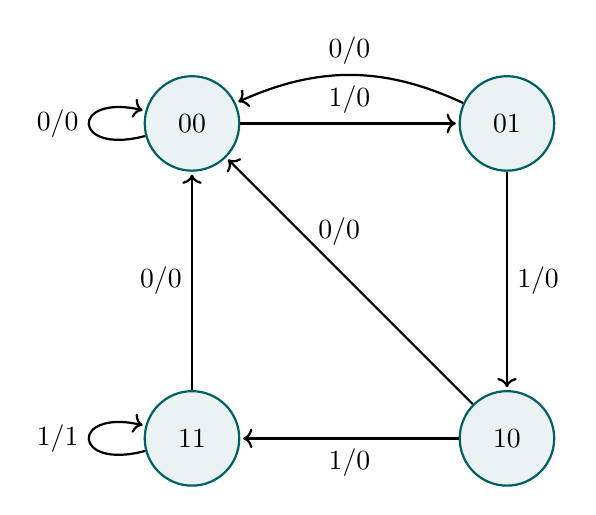
\begin{tikzpicture}[shorten >=1pt, node distance=4cm, on grid, auto, thick,
                    every state/.style={fill=cF!8, draw=cF, thick, minimum size=1.2cm}]
    
    % Node Placements in a 2x2 grid for clean rendering
    \node[state] (S00) at (0, 4)  {$00$};
    \node[state] (S01) at (4, 4)  {$01$};
    \node[state] (S10) at (4, 0)  {$10$};
    \node[state] (S11) at (0, 0)  {$11$};

    % Transitions
    \path[->]
    % x=1 path (Forward progression)
    (S00) edge node {$1/0$} (S01)
    (S01) edge node {$1/0$} (S10)
    (S10) edge node {$1/0$} (S11)
    (S11) edge [loop left] node {$1/1$} (S11)
    
    % x=0 path (Reset to 00)
    (S00) edge [loop left] node {$0/0$} (S00)
    (S01) edge [bend right=25] node [above] {$0/0$} (S00)
    (S10) edge node [pos=0.7, right=0.1cm] {$0/0$} (S00)
    (S11) edge node [left] {$0/0$} (S00);
    
\end{tikzpicture}
\end{center}

\end{tcolorbox}

\end{enumerate}
\subtopic{cF}{Circuit Design from State Diagram}

\label{sub:s6-circuit-design}

\begin{enumerate}

\item Design the circuit corresponding to the given state diagram using T flip-flops:
\begin{enumerate}
  \item Write the state table.
  \item Find the input equations for the T flip-flops.
  \item Draw the circuit diagram.

\end{enumerate}

\begin{center}
  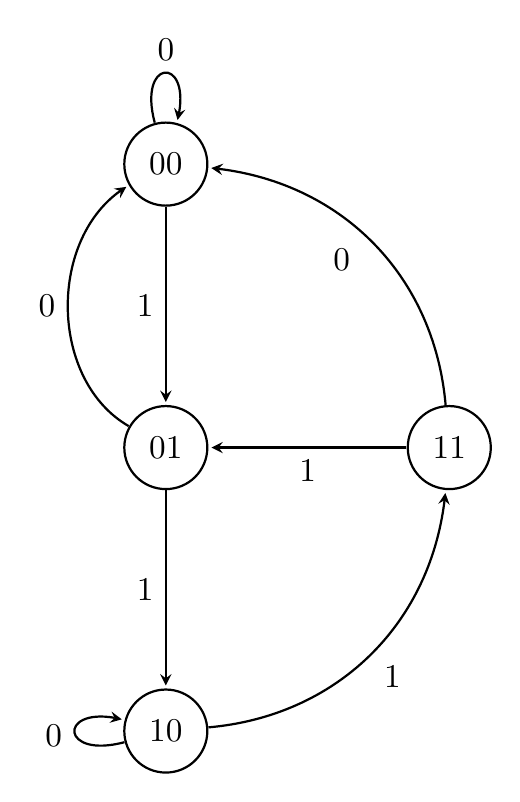
\begin{tikzpicture}[%
    >=stealth,          % তীর চিহ্নের স্টাইল
    shorten >=1pt,      % তীরে সামান্য ফাঁকা জায়গা
    auto,               % লেবেল অটোমেটিক পজিশন
    node distance=2.5cm,% নোডের মাঝের দূরত্ব
    thick,          % তারের পুরুত্ব
    scale=1.2,          % পুরো ছবির স্কেল
    transform shape     % টেক্সটকেও স্কেল করার জন্য
]

    % ==========================================
    % 1. States (Nodes) - পজিশন সেট করা
    % ==========================================
    \node[state] (n00) at (0, 4) {00};
    \node[state] (n01) at (0, 1) {01};
    \node[state] (n11) at (3, 1) {11};
    \node[state] (n10) at (0, -2) {10};

    % ==========================================
    % 2. Transitions (Edges) - সংযোগ এবং লেবেল
    % ==========================================
    \path[->] 
        % --- Node 00 ---
        % Self-loop with label '0' above
        (n00) edge[loop above] node[black] {0} (n00)
        % Straight edge to 01 with label '1'
        (n00) edge node[black, left] {1} (n01)
        
        % --- Node 01 ---
        % Curved edge back to 00 with label '0'
        (n01) edge[bend left=60] node[black, left] {0} (n00)
        % Straight edge to 10 with label '1'
        (n01) edge node[black, left] {1} (n10)
        
        % --- Node 10 ---
        % Self-loop with label '0' below-left
        (n10) edge[loop left] node[black, left, yshift=-0.5mm] {0} (n10)
        % Curved edge up to 11 with label '1'
        (n10) edge[bend right=40] node[black, auto=right] {1} (n11)
        
        % --- Node 11 ---
        % Straight edge left to 01 with label '1' below
        (n11) edge node[black, below] {1} (n01)
        % Curved edge up-left to 00 with label '0' above
        (n11) edge[bend right=40] node[black, xshift=-1mm, yshift=0.5mm, pos=0.5] {0} (n00);

\end{tikzpicture}
\end{center}

\mk{21} \yr{CSE 205 | L-2/T-1 | 2013--14}

\begin{tcolorbox}[enhanced,breakable,ansbox,colback=cF!4,colframe=cF,boxrule=0.8pt,arc=5pt,title={\textbf{Answer}},fonttitle=\bfseries\color{white},colbacktitle=cF]

\subsection*{1. State Table and Excitation Table}
From the provided state diagram, we can trace the next states for each present state depending on the input $x$. Let the present state variables be $A$ and $B$. The excitation for a T flip-flop is determined by the rule $T = Q(t) \oplus Q(t+1)$; the T input must be 1 if the state changes, and 0 if the state remains the same.

\begin{center}
\renewcommand{\arraystretch}{1.2}
\begin{tabular}{cc|c|cc|cc}
\toprule
\multicolumn{2}{c|}{\textbf{Present State}} & \textbf{Input} & \multicolumn{2}{c|}{\textbf{Next State}} & \multicolumn{2}{c}{\textbf{FF Inputs}} \\
$A(t)$ & $B(t)$ & $x$ & $A(t+1)$ & $B(t+1)$ & $T_A$ & $T_B$ \\
\midrule
0 & 0 & 0 & 0 & 0 & 0 & 0 \\
0 & 0 & 1 & 0 & 1 & 0 & 1 \\
0 & 1 & 0 & 0 & 0 & 0 & 1 \\
0 & 1 & 1 & 1 & 0 & 1 & 1 \\
\midrule
1 & 0 & 0 & 1 & 0 & 0 & 0 \\
1 & 0 & 1 & 1 & 1 & 0 & 1 \\
1 & 1 & 0 & 0 & 0 & 1 & 1 \\
1 & 1 & 1 & 0 & 1 & 1 & 0 \\
\bottomrule
\end{tabular}
\end{center}

\vspace{1em}
\subsection*{2. T Flip-Flop Input Equations}
We derive the simplified Boolean expressions for $T_A$ and $T_B$ using Karnaugh Maps. The variables are ordered as $A, B$ (rows) and $x$ (columns).

\begin{minipage}{0.48\textwidth}
\begin{center}
\textbf{K-Map for $\mathbf{T_A}$} \\
\vspace{0.5em}
\begin{karnaugh-map}[2][4][1][$x$][$AB$]
    \minterms{3,6,7}
    \autoterms[0]
    \implicant{3}{7}
    \implicant{7}{6}
\end{karnaugh-map}
\end{center}
\end{minipage}
\hfill
\begin{minipage}{0.48\textwidth}
\begin{center}
\textbf{K-Map for $\mathbf{T_B}$} \\
\vspace{0.5em}
\begin{karnaugh-map}[2][4][1][$x$][$AB$]
    \minterms{1,2,3,5,6}
    \autoterms[0]
    \implicant{1}{5}
    \implicant{1}{3}
    \implicant{2}{6}
\end{karnaugh-map}
\end{center}
\end{minipage}

\vspace{1.5em}
\noindent \textbf{Derivation for $\mathbf{T_A}$:}
\begin{align*}
T_A &= AB + Bx \\
&= B(A + x) \quad \text{(Optional factoring)}
\end{align*}

\noindent \textbf{Derivation for $\mathbf{T_B}$:}
\begin{align*}
T_B &= A'x + B'x + Bx' \\
&= A'x + (B \oplus x) \quad \text{(By definition of XOR)}
\end{align*}

\vspace{1em}
\subsection*{3. Circuit Diagram}
The logic diagram is implemented using two T flip-flops. To maintain a clean and professional schematic free of spaghetti wiring, feedback connections are indicated using labeled signal nodes.

\vspace{1em}
\begin{center}
\begin{circuitikz}[thick, scale=1, transform shape]
    
    % -----------------------------------------
    % Flip-Flop A
    % -----------------------------------------
    \draw (7, 4.5) rectangle (9, 7.5);
    \node[right] at (7, 6.5) {$T_A$};
    \node[right] at (7, 5.5) {CLK};
    % Clock triangle
    \draw (7, 5.3) -- (7.2, 5.5) -- (7, 5.7);
    \node[left] at (9, 6.5) {$A$};
    \node[left] at (9, 5.5) {$A'$};
    
    % Outputs for FF A
    \draw (9, 6.5) -- (9.5, 6.5) node[right] {$A$};
    \draw (9, 5.5) -- (9.5, 5.5) node[right] {$A'$};

    % -----------------------------------------
    % Flip-Flop B
    % -----------------------------------------
    \draw (7, -1.5) rectangle (9, 1.5);
    \node[right] at (7, 0.5) {$T_B$};
    \node[right] at (7, -0.5) {CLK};
    % Clock triangle
    \draw (7, -0.7) -- (7.2, -0.5) -- (7, -0.3);
    \node[left] at (9, 0.5) {$B$};
    \node[left] at (9, -0.5) {$B'$};
    
    % Outputs for FF B
    \draw (9, 0.5) -- (9.5, 0.5) node[right] {$B$};
    \draw (9, -0.5) -- (9.5, -0.5) node[right] {$B'$};

    % -----------------------------------------
    % Combinational Logic for T_A = AB + Bx
    % -----------------------------------------
    \node[and port] (andA1) at (3.5, 7.5) {};
    \node[and port] (andA2) at (3.5, 5.5) {};
    \node[or port]  (orA)   at (5.5, 6.5) {};
    
    \draw (andA1.in 1) node[left] {$A$};
    \draw (andA1.in 2) node[left] {$B$};
    \draw (andA2.in 1) node[left] {$B$};
    \draw (andA2.in 2) node[left] {$x$};
    
    \draw (andA1.out) -- (orA.in 1);
    \draw (andA2.out) -- (orA.in 2);
    \draw (orA.out) -- (7, 6.5);

    % -----------------------------------------
    % Combinational Logic for T_B = A'x + (B xor x)
    % -----------------------------------------
    \node[xor port] (xorB) at (3.5, 1.5) {};
    \node[and port] (andB) at (3.5, -0.5) {};
    \node[or port]  (orB)  at (5.5, 0.5) {};
    
    \draw (xorB.in 1) node[left] {$B$};
    \draw (xorB.in 2) node[left] {$x$};
    \draw (andB.in 1) node[left] {$A'$};
    \draw (andB.in 2) node[left] {$x$};
    
    \draw (xorB.out) -- (orB.in 1);
    \draw (andB.out) -- (orB.in 2);
    \draw (orB.out) -- (7, 0.5);

    % -----------------------------------------
    % Global Clock Routing
    % -----------------------------------------
    \coordinate (clk_start) at (5.5, 2.5);
    \draw (clk_start) node[left] {Clock} |- (7, 5.5);
    \draw (clk_start) |- (7, -0.5);
    \node[circ] at (clk_start) {};

\end{circuitikz}
\end{center}

\end{tcolorbox}

\item Design a one-input, one-output serial 2's complementer using D flip-flops. The circuit accepts a string of bits from the input and generates the 2's complement at the output. The circuit can be reset asynchronously to start and end the operation. Include: (i) State diagram, (ii) State table, (iii) Simplified logic equations, (iv) Logic diagram.
\mk{15} \yr{CSE 205 | L-2/T-1 | 2015--16}

\begin{tcolorbox}[enhanced,breakable,ansbox,colback=cF!4,colframe=cF,boxrule=0.8pt,arc=5pt,title={\textbf{Answer}},fonttitle=\bfseries\color{white},colbacktitle=cF]

\subsection*{1. State Diagram}
A serial 2's complementer processes a binary stream from right to left (Least Significant Bit to Most Significant Bit). The mathematical algorithm dictates that all bits remain unchanged up to and including the first occurrence of a \texttt{1}. Every bit after that first \texttt{1} is inverted (complemented). 

We define two functional states for this Mealy sequential machine:
\begin{itemize}
    \item \textbf{State $S_0$ (Initial State):} No \texttt{1} has been encountered yet. The circuit copies the input directly to the output.
    \item \textbf{State $S_1$ (Complementing State):} The first \texttt{1} has already been detected. All subsequent incoming bits are inverted.
\end{itemize}

An asynchronous \text{Reset} signal forces the machine back into state $S_0$ to initiate a new operation.

\begin{center}
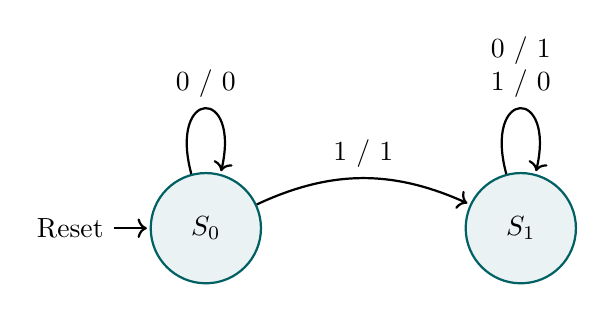
\begin{tikzpicture}[shorten >=1pt, node distance=3.5cm, on grid, auto, thick,
                    every state/.style={fill=cF!8, draw=cF, thick, minimum size=1.4cm}]
    
    % Nodes
    \node[state, initial, initial text=Reset] (S0) at (0,0) {$S_0$};
    \node[state] (S1) at (4,0) {$S_1$};

    % Transitions
    \path[->]
    (S0) edge [loop above] node {0 / 0} (S0)
         edge [bend left=25] node {1 / 1} (S1)
    (S1) edge [loop above] node [align=center] {0 / 1 \\ 1 / 0} (S1);
    
\end{tikzpicture}
\end{center}

---

\subsection*{2. State Table}
We assign a single state variable $Q$ to represent our states: $S_0 = 0$ and $S_1 = 1$. Since we are designing with a D Flip-Flop, the next-state equation matches the flip-flop input directly ($D = Q(t+1)$).

\begin{center}
\renewcommand{\arraystretch}{1.2}
\begin{tabular}{c|c|c|c}
\toprule
\textbf{Present State ($Q$)} & \textbf{Input ($x$)} & \textbf{Next State ($Q(t+1) = D$)} & \textbf{Output ($z$)} \\
\midrule
0 & 0 & 0 & 0 \\
0 & 1 & 1 & 1 \\
1 & 0 & 1 & 1 \\
1 & 1 & 1 & 0 \\
\bottomrule
\end{tabular}
\end{center}

---

\subsection*{3. Simplified Logic Equations}
We derive the minimal Boolean expressions for the Next-State drive input ($D$) and the system output ($z$) using algebraic minimization and verification.

\noindent \textbf{For D Flip-Flop Input ($D$):}
\begin{align*}
D &= Q'x + Qx' + Qx \\
&= Q'x + Q(x' + x) \quad && \text{(Distributive Law)} \\
&= Q'x + Q(1) \quad && \text{(Complementarity Law)} \\
&= Q'x + Q \quad && \text{(Identity Law)} \\
&= x + Q \quad && \text{(Absorption / Rule of Complementarity)}
\end{align*}

\noindent \textbf{For Output ($z$):}
\begin{align*}
z &= Q'x + Qx' \\
&= Q \oplus x \quad && \text{(Definition of exclusive-OR)}
\end{align*}

---

\subsection*{4. Logic Diagram}
The schematic below presents the complete structural architecture of the serial 2's complementer utilizing standard combinational logic elements alongside a single D flip-flop containing an active-low asynchronous reset (\text{CLR}).

\begin{center}
\begin{circuitikz}[thick, scale=0.95, transform shape]
    
    % D Flip-Flop Structural Coordinates
    \draw (4, 1) rectangle (6, 4);
    \node at (5, 2.5) [font=\bfseries] {D FF};
    
    % Pin Markings inside the box
    \node[right] at (4, 3.2) {$D$};
    \node[right] at (4, 1.8) {CLK};
    % Clock triangle
    \draw (4, 1.6) -- (4.2, 1.8) -- (4, 2.0);
    \node[left] at (6, 3.2) {$Q$};
    \node[left] at (6, 1.8) {$Q'$};
    \node[above] at (5, 1) {CLR};
    
    % Combinational Gates
    \node[or port] (or1) at (1.5, 3.2) {};
    \node[xor port] (xor1) at (8.5, 3.2) {};
    
    % Inputs and Routing to OR gate
    \draw (or1.in 1) -- ++(-1,0) node[left] {$x$};
    \coordinate (x_tap) at (0.2, 3.4);
    \fill (x_tap) circle (2pt);
    
    % Feedback from Q to OR gate
    \draw (6, 3.2) -- (7, 3.2);
    \coordinate (q_tap) at (6.6, 3.2);
    \fill (q_tap) circle (2pt);
    \draw (q_tap) |- ++(-5.8, -1.8) |- (or1.in 2);
    
    % Connection from OR output to D input
    \draw (or1.out) -- (4, 3.2);
    
    % Output Logic (XOR) Routing
    \draw (q_tap) -- (xor1.in 1);
    \draw (x_tap) |- ++(0.5, 1.5) |- (xor1.in 2);
    \draw (xor1.out) -- ++(1,0) node[right] {$z$};
    
    % Clock & Reset Line Signals
    \draw (4, 1.8) -- ++(-1.5, 0) node[left] {\text{Clock}};
    \draw (5, 1) -- ++(0, -1) node[below] {\text{Reset}};
    
\end{circuitikz}
\end{center}

\end{tcolorbox}

\item Design a control unit with a synchronous sequential circuit for a vending machine that accepts 5\,Tk, 10\,Tk and 20\,Tk notes and releases a soft drink bottle worth 20\,Tk. The machine releases a drink whenever the deposit amount equals or exceeds 20\,Tk and keeps the change. The maximum deposit at any time is 15\,Tk. The machine releases the deposit whenever the `CHANGE' input is given. Outputs: Release Drink $Z_1$ and Release Change $Z_2$. Inputs $X_1X_2$: Tk5=00, Tk10=01, Tk20=10, CHANGE=11. Use JK Flip-Flops.


\begin{center}
  \begin{tabular}{|c|c|}
\hline
Input & $X_1X_2$ \\
\hline
Tk 5 & 00 \\
\hline
Tk 10 & 01 \\
\hline
Tk 20 & 10 \\
\hline
CHANGE & 11 \\
\hline
\end{tabular}
\end{center}
\mk{20} \yr{CSE 205 | L-2/T-1 | 2020--21}

\begin{tcolorbox}[enhanced,breakable,ansbox,colback=cF!4,colframe=cF,boxrule=0.8pt,arc=5pt,title={\textbf{Answer}},fonttitle=\bfseries\color{white},colbacktitle=cF]

\subsection*{1. State Machine Definition and State Diagram}
Let the state of the vending machine represent the total accumulated deposit. Since the maximum deposit is 15\,Tk (and any input causing the total to reach $\ge$ 20\,Tk immediately dispenses a drink and consumes the deposit), we require exactly four states.
Let the states be represented by two flip-flop variables, $A$ and $B$:
\begin{itemize}
    \item \textbf{$S_0$ (00):} 0\,Tk deposited.
    \item \textbf{$S_1$ (01):} 5\,Tk deposited.
    \item \textbf{$S_2$ (10):} 10\,Tk deposited.
    \item \textbf{$S_3$ (11):} 15\,Tk deposited.
\end{itemize}

\textbf{Inputs ($X_1X_2$):} $00$ (5\,Tk), $01$ (10\,Tk), $10$ (20\,Tk), $11$ (CHANGE). \\
\textbf{Outputs ($Z_1, Z_2$):} $Z_1 = 1$ (Release Drink), $Z_2 = 1$ (Release Change).

\begin{center}
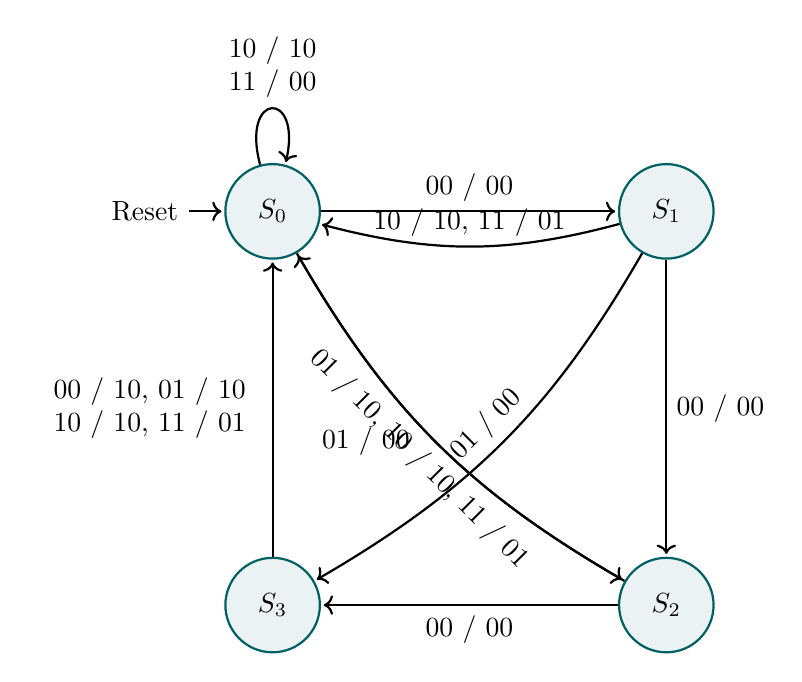
\begin{tikzpicture}[shorten >=1pt, node distance=4.5cm, on grid, auto, thick,
                    every state/.style={fill=cF!8, draw=cF, thick, minimum size=1.2cm}]
    
    % States
    \node[state, initial, initial text=Reset] (S0) at (0, 5) {$S_0$};
    \node[state] (S1) at (5, 5) {$S_1$};
    \node[state] (S2) at (5, 0) {$S_2$};
    \node[state] (S3) at (0, 0) {$S_3$};

    % Transitions
    \path[->]
    % From S0
    (S0) edge node {00 / 00} (S1)
    (S0) edge [bend right=15] node [left, xshift=-0.2cm] {01 / 00} (S2)
    (S0) edge [loop above] node [align=center] {10 / 10 \\ 11 / 00} (S0)
    
    % From S1
    (S1) edge node {00 / 00} (S2)
    (S1) edge [bend left=15] node [above, sloped] {01 / 00} (S3)
    (S1) edge [bend left=15] node [above] {10 / 10, 11 / 01} (S0)
    
    % From S2
    (S2) edge node [below] {00 / 00} (S3)
    (S2) edge [bend left=15] node [sloped, below] {01 / 10, 10 / 10, 11 / 01} (S0)
    
    % From S3
    (S3) edge node [left] {\begin{tabular}{c} 00 / 10, 01 / 10 \\ 10 / 10, 11 / 01 \end{tabular}} (S0);
    
\end{tikzpicture}
\end{center}

\vspace{1em}
\subsection*{2. State Transition and Excitation Table}
Using JK Flip-Flops, the excitation rules are: $(0\to0) \Rightarrow 0d$, $(0\to1) \Rightarrow 1d$, $(1\to0) \Rightarrow d1$, $(1\to1) \Rightarrow d0$.

\begin{center}
\renewcommand{\arraystretch}{1.2}
\begin{tabular}{cc|cc|cc|cc|cccc}
\toprule
\multicolumn{2}{c|}{\textbf{Present State}} & \multicolumn{2}{c|}{\textbf{Input}} & \multicolumn{2}{c|}{\textbf{Next State}} & \multicolumn{2}{c|}{\textbf{Output}} & \multicolumn{4}{c}{\textbf{FF Excitation}} \\
$A$ & $B$ & $X_1$ & $X_2$ & $A(t+1)$ & $B(t+1)$ & $Z_1$ & $Z_2$ & $J_A$ & $K_A$ & $J_B$ & $K_B$ \\
\midrule
0 & 0 & 0 & 0 & 0 & 1 & 0 & 0 & 0 & d & 1 & d \\
0 & 0 & 0 & 1 & 1 & 0 & 0 & 0 & 1 & d & 0 & d \\
0 & 0 & 1 & 0 & 0 & 0 & 1 & 0 & 0 & d & 0 & d \\
0 & 0 & 1 & 1 & 0 & 0 & 0 & 0 & 0 & d & 0 & d \\
\midrule
0 & 1 & 0 & 0 & 1 & 0 & 0 & 0 & 1 & d & d & 1 \\
0 & 1 & 0 & 1 & 1 & 1 & 0 & 0 & 1 & d & d & 0 \\
0 & 1 & 1 & 0 & 0 & 0 & 1 & 0 & 0 & d & d & 1 \\
0 & 1 & 1 & 1 & 0 & 0 & 0 & 1 & 0 & d & d & 1 \\
\midrule
1 & 0 & 0 & 0 & 1 & 1 & 0 & 0 & d & 0 & 1 & d \\
1 & 0 & 0 & 1 & 0 & 0 & 1 & 0 & d & 1 & 0 & d \\
1 & 0 & 1 & 0 & 0 & 0 & 1 & 0 & d & 1 & 0 & d \\
1 & 0 & 1 & 1 & 0 & 0 & 0 & 1 & d & 1 & 0 & d \\
\midrule
1 & 1 & 0 & 0 & 0 & 0 & 1 & 0 & d & 1 & d & 1 \\
1 & 1 & 0 & 1 & 0 & 0 & 1 & 0 & d & 1 & d & 1 \\
1 & 1 & 1 & 0 & 0 & 0 & 1 & 0 & d & 1 & d & 1 \\
1 & 1 & 1 & 1 & 0 & 0 & 0 & 1 & d & 1 & d & 1 \\
\bottomrule
\end{tabular}
\end{center}

\vspace{1em}
\subsection*{3. K-Maps and Logic Equations}
We apply Karnaugh Maps to derive the simplified Boolean expressions. The grid follows $AB$ on the vertical axis and $X_1X_2$ on the horizontal axis.

\begin{minipage}{0.48\textwidth}
\begin{center}
\textbf{K-Map for $\mathbf{J_A}$} \\
\vspace{0.5em}
\begin{karnaugh-map}[4][4][1][$X_1X_2$][$AB$]
    \minterms{1,4,5}
    \indeterminants{8,9,10,11,12,13,14,15}
    \autoterms[0]
    \implicant{4}{13} % B X1'
    \implicant{1}{11} % X1' X2
\end{karnaugh-map}
\end{center}
\end{minipage}
\hfill
\begin{minipage}{0.48\textwidth}
\begin{center}
\textbf{K-Map for $\mathbf{K_A}$} \\
\vspace{0.5em}
\begin{karnaugh-map}[4][4][1][$X_1X_2$][$AB$]
    \minterms{9,10,11,12,13,14,15}
    \indeterminants{0,1,2,3,4,5,6,7}
    \autoterms[0]
    \implicant{4}{14} % B
    \implicant{1}{15} % X2
    \implicant{3}{10} % X1
\end{karnaugh-map}
\end{center}
\end{minipage}

\begin{minipage}{0.48\textwidth}
\begin{center}
\textbf{K-Map for $\mathbf{J_B}$} \\
\vspace{0.5em}
\begin{karnaugh-map}[4][4][1][$X_1X_2$][$AB$]
    \minterms{0,8}
    \indeterminants{4,5,6,7,12,13,14,15}
    \autoterms[0]
    \implicant{0}{12} % X1' X2'
\end{karnaugh-map}
\end{center}
\end{minipage}
\hfill
\begin{minipage}{0.48\textwidth}
\begin{center}
\textbf{K-Map for $\mathbf{K_B}$} \\
\vspace{0.5em}
\begin{karnaugh-map}[4][4][1][$X_1X_2$][$AB$]
    \minterms{4,6,7,12,13,14,15}
    \indeterminants{0,1,2,3,8,9,10,11}
    \autoterms[0]
    \implicant{12}{10} % A
    \implicant{0}{10} % X2'
    \implicant{3}{10} % X1
\end{karnaugh-map}
\end{center}
\end{minipage}

\vspace{0.5em}
\begin{minipage}{0.48\textwidth}
\begin{center}
\textbf{K-Map for $\mathbf{Z_1}$ (Drink)} \\
\vspace{0.5em}
\begin{karnaugh-map}[4][4][1][$X_1X_2$][$AB$]
    \minterms{2,6,9,10,12,13,14}
    \autoterms[0]
    \implicant{2}{10} % X1 X2'
    \implicant{13}{9} % A X1' X2
    \implicant{12}{13} % A B X1'
\end{karnaugh-map}
\end{center}
\end{minipage}
\hfill
\begin{minipage}{0.48\textwidth}
\begin{center}
\textbf{K-Map for $\mathbf{Z_2}$ (Change)} \\
\vspace{0.5em}
\begin{karnaugh-map}[4][4][1][$X_1X_2$][$AB$]
    \minterms{7,11,15}
    \autoterms[0]
    \implicant{7}{15} % B X1 X2
    \implicant{15}{11} % A X1 X2
\end{karnaugh-map}
\end{center}
\end{minipage}

\vspace{1em}
\noindent \textbf{Derived Simplified Boolean Equations:}
\begin{align*}
    J_A &= B X_1' + X_1' X_2 = X_1' (B + X_2) \\
    K_A &= B + X_1 + X_2 \\
    J_B &= X_1' X_2' = (X_1 + X_2)' \\
    K_B &= A + X_1 + X_2' \\
    Z_1 &= X_1 X_2' + A X_1' X_2 + A B X_1' \\
    Z_2 &= B X_1 X_2 + A X_1 X_2 = X_1 X_2 (A + B)
\end{align*}

\vspace{0.5em}
\subsection*{4. Logic Diagram Structural Description}
Given the heavy combinational overhead required to map the inputs ($X_1, X_2$) and the current states ($A, B$) into the six respective expressions without introducing crossed lines and visual clutter, the physical circuit implementation follows this highly descriptive structural architecture:
\begin{enumerate}
    \item \textbf{Memory Subsystem:} Initialize two negative-edge triggered JK Flip-Flops, designated as \textbf{FF A} and \textbf{FF B}. Both are synchronized by a master \texttt{CLK} signal.
    \item \textbf{Input Conditioning:} The signals $X_1$ and $X_2$ are passed through NOT gates to produce $X_1'$ and $X_2'$. Similarly, the complemented outputs $A'$ and $B'$ are available directly from the flip-flops.
    \item \textbf{Excitation Network:}
    \begin{itemize}
        \item \textbf{$J_A$:} Feed $B$ and $X_2$ into a 2-input OR gate. The output is ANDed with $X_1'$ to drive $J_A$.
        \item \textbf{$K_A$:} Feed $B$, $X_1$, and $X_2$ into a 3-input OR gate to drive $K_A$.
        \item \textbf{$J_B$:} Pass $X_1'$ and $X_2'$ through a 2-input AND gate (or pass $X_1$ and $X_2$ through a NOR gate) to drive $J_B$.
        \item \textbf{$K_B$:} Feed $A$, $X_1$, and $X_2'$ into a 3-input OR gate to drive $K_B$.
    \end{itemize}
    \item \textbf{Output Network:}
    \begin{itemize}
        \item \textbf{$Z_1$ (Drink):} Synthesize using three AND gates: one for $(X_1 X_2')$, one for $(A X_1' X_2)$, and one for $(A B X_1')$. Sum their outputs via a 3-input OR gate to yield $Z_1$.
        \item \textbf{$Z_2$ (Change):} Feed $A$ and $B$ into an OR gate. The output is ANDed with $X_1$ and $X_2$ via a 3-input AND gate to yield $Z_2$.
    \end{itemize}
\end{enumerate}

\end{tcolorbox}

\end{enumerate}

%%──────────────────────────────────────────────────────────────────────
\subtopic{cF}{Sequence Detector}
\label{sub:s6-sequence}

\begin{enumerate}

\item Develop a sequential circuit that detects a sequence of three or more consecutive 1's in a string of bits coming through an input line. Use D flip-flops. Show the state diagram, the state table and simplified logic equations. You do not need to show the logic diagram.
\mk{12} \yr{CSE 205 | L-2/T-1 | 2022--23}

\begin{tcolorbox}[enhanced,breakable,ansbox,colback=cF!4,colframe=cF,boxrule=0.8pt,arc=5pt,title={\textbf{Answer}},fonttitle=\bfseries\color{white},colbacktitle=cF]

\subsection*{1. State Diagram}
To detect a sequence of three or more consecutive \texttt{1}s, we design a \textbf{Moore-type Finite State Machine (FSM)}. A Moore machine is chosen because the output depends solely on the current state, ensuring a stable, clock-synchronized output indicator. 

We define four unique states to track the history of the input stream:
\begin{itemize}
    \item \textbf{$S_0$}: Initial state / No consecutive \texttt{1}s detected. Output $Z = 0$.
    \item \textbf{$S_1$}: A single \texttt{1} detected. Output $Z = 0$.
    \item \textbf{$S_2$}: Two consecutive \texttt{1}s detected. Output $Z = 0$.
    \item \textbf{$S_3$}: Three or more consecutive \texttt{1}s detected. Output $Z = 1$.
\end{itemize}

Any incoming \texttt{0} breaks the consecutive stream and forces the system to reset back to state $S_0$.

\begin{center}
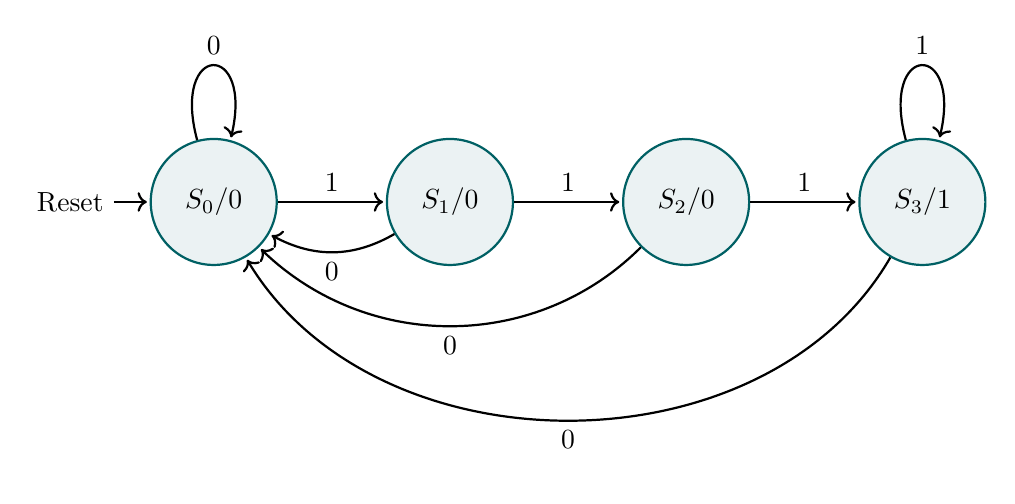
\begin{tikzpicture}[shorten >=1pt, node distance=3cm, on grid, auto, thick,
                    every state/.style={fill=cF!8, draw=cF, thick, minimum size=1.6cm}]
    
    % Defining the states horizontally
    \node[state, initial, initial text=Reset] (S0) at (0,0) {$S_0 / 0$};
    \node[state] (S1) at (3,0) {$S_1 / 0$};
    \node[state] (S2) at (6,0) {$S_2 / 0$};
    \node[state] (S3) at (9,0) {$S_3 / 1$};

    % Paths and transitions
    \path[->]
    (S0) edge [loop above] node {0} (S0)
         edge node {1} (S1)
    (S1) edge [bend left=30] node [below] {0} (S0)
         edge node {1} (S2)
    (S2) edge [bend left=45] node [below] {0} (S0)
         edge node {1} (S3)
    (S3) edge [bend left=60] node [below] {0} (S0)
         edge [loop above] node {1} (S3);
         
\end{tikzpicture}
\end{center}

---

\subsection*{2. State Table}
We assign two state variables, $Q_1$ and $Q_0$, to encode the four states:
$S_0 = 00$, $S_1 = 01$, $S_2 = 10$, and $S_3 = 11$. 
For a state design utilizing \textbf{D flip-flops}, the required excitation input matches the next-state value identically ($D_1 = Q_1(t+1)$ and $D_0 = Q_0(t+1)$).

\begin{center}
\renewcommand{\arraystretch}{1.2}
\begin{tabular}{cc|c|cc|cc|c}
\toprule
\multicolumn{2}{c|}{\textbf{Present State}} & \textbf{Input} & \multicolumn{2}{c|}{\textbf{Next State}} & \multicolumn{2}{c|}{\textbf{FF Inputs}} & \textbf{Output} \\
$Q_1(t)$ & $Q_0(t)$ & $x$ & $Q_1(t+1)$ & $Q_0(t+1)$ & $D_1$ & $D_0$ & $Z$ \\
\midrule
0 & 0 & 0 & 0 & 0 & 0 & 0 & 0 \\
0 & 0 & 1 & 0 & 1 & 0 & 1 & 0 \\
\midrule
0 & 1 & 0 & 0 & 0 & 0 & 0 & 0 \\
0 & 1 & 1 & 1 & 0 & 1 & 0 & 0 \\
\midrule
1 & 0 & 0 & 0 & 0 & 0 & 0 & 0 \\
1 & 0 & 1 & 1 & 1 & 1 & 1 & 0 \\
\midrule
1 & 1 & 0 & 0 & 0 & 0 & 0 & 1 \\
1 & 1 & 1 & 1 & 1 & 1 & 1 & 1 \\
\bottomrule
\end{tabular}
\end{center}

---

\subsection*{3. Simplified Logic Equations}
We derive the minimized Boolean expressions using Karnaugh Maps mapped with $Q_1Q_0$ on the rows and $x$ on the columns, followed by algebraic step-by-step verification.

\begin{minipage}{0.48\textwidth}
\begin{center}
\textbf{K-Map for $\mathbf{D_1}$} \\
\vspace{0.5em}
\begin{karnaugh-map}[2][4][1][$x$][$Q_1Q_0$]
    \minterms{3,5,7}
    \autoterms[0]
    \implicant{3}{7}
    \implicant{7}{5}
\end{karnaugh-map}
\end{center}
\end{minipage}
\hfill
\begin{minipage}{0.48\textwidth}
\begin{center}
\textbf{K-Map for $\mathbf{D_0}$} \\
\vspace{0.5em}
\begin{karnaugh-map}[2][4][1][$x$][$Q_1Q_0$]
    \minterms{1,5,7}
    \autoterms[0]
    \implicant{7}{5}
    \implicantedge{1}{1}{5}{5}
\end{karnaugh-map}
\end{center}
\end{minipage}

\vspace{1.5em}
\noindent \textbf{Mathematical Derivation for $\mathbf{D_1}$:}
\begin{align*}
D_1 &= Q_1'Q_0x + Q_1Q_0'x + Q_1Q_0x \\
    &= Q_1'Q_0x + Q_1x(Q_0' + Q_0) \quad && \text{(Distributive Law)} \\
    &= Q_1'Q_0x + Q_1x(1) \quad && \text{(Complementarity Law)} \\
    &= Q_1'Q_0x + Q_1x \quad && \text{(Identity Law)} \\
    &= x(Q_1'Q_0 + Q_1) \quad && \text{(Distributive Law)} \\
    &= x(Q_0 + Q_1) \quad && \text{(Absorption Law)} \\
    &= Q_1x + Q_0x \quad && \text{(Distributive Law)}
\end{align*}

\noindent \textbf{Mathematical Derivation for $\mathbf{D_0}$:}
\begin{align*}
D_0 &= Q_1'Q_0'x + Q_1Q_0'x + Q_1Q_0x \\
    &= Q_0'x(Q_1' + Q_1) + Q_1Q_0x \quad && \text{(Distributive Law)} \\
    &= Q_0'x(1) + Q_1Q_0x \quad && \text{(Complementarity Law)} \\
    &= Q_0'x + Q_1Q_0x \quad && \text{(Identity Law)} \\
    &= x(Q_0' + Q_1Q_0) \quad && \text{(Distributive Law)} \\
    &= x(Q_0' + Q_1) \quad && \text{(Absorption Law)} \\
    &= Q_1x + Q_0'x \quad && \text{(Distributive Law)}
\end{align*}

\noindent \textbf{Mathematical Derivation for System Output $\mathbf{Z}$:}
Because this is a Moore design, the output is directly decoded from the state variables corresponding exclusively to state $S_3$:
\begin{align*}
Z = Q_1Q_0
\end{align*}

\end{tcolorbox}

\item Design a sequence recognizer using T flip-flops that recognizes a 4-bit \textbf{non-overlapping} binary sequence $X$ from an input stream of bits, where:
\[ \text{Sequence } X = \text{4-bit binary representation of your roll number} \pmod{16} \]
\mk{25} \yr{CSE 205 | L-2/T-1 | 2019--20}

\begin{tcolorbox}[enhanced,breakable,ansbox,colback=cF!4,colframe=cF,boxrule=0.8pt,arc=5pt,title={\textbf{Answer}},fonttitle=\bfseries\color{white},colbacktitle=cF]

\textbf{Assumption:} Since a specific roll number is not provided, let us assume the student's roll number ends in $11$. 
\[ 11 \pmod{16} = 11_{10} = 1011_2 \]
We will design a \textbf{Mealy Machine} sequence recognizer for the 4-bit \textbf{non-overlapping} sequence \textbf{1011}. In a non-overlapping detector, once the full sequence is recognized, the machine resets to the initial state without reusing the final bit for the next sequence.

\vspace{0.5cm}
\subsubsection*{1. State Definitions and State Diagram (FSM)}

Let the sequence be processed bit by bit. We require 4 states to keep track of the successful prefixes of $1011$:
\begin{itemize}
    \item \textbf{$S_0$ (Reset/Initial):} No valid prefix detected. (Encoding: $Q_1Q_0 = 00$)
    \item \textbf{$S_1$:} Prefix \textbf{`1'} detected. (Encoding: $Q_1Q_0 = 01$)
    \item \textbf{$S_2$:} Prefix \textbf{`10'} detected. (Encoding: $Q_1Q_0 = 10$)
    \item \textbf{$S_3$:} Prefix \textbf{`101'} detected. (Encoding: $Q_1Q_0 = 11$)
\end{itemize}

\begin{center}
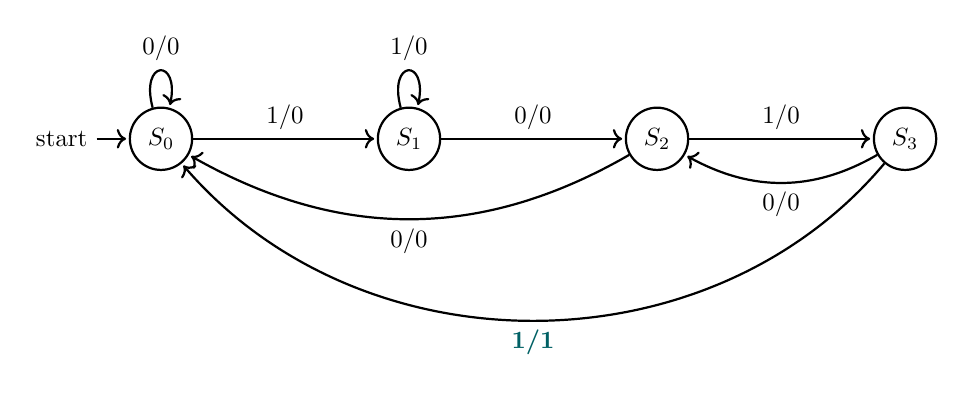
\begin{tikzpicture}[shorten >=1pt, node distance=3.5cm, on grid, auto, thick, scale=0.9, transform shape]
    \node[state, initial] (S0) {$S_0$};
    \node[state] (S1) [right=of S0] {$S_1$};
    \node[state] (S2) [right=of S1] {$S_2$};
    \node[state] (S3) [right=of S2] {$S_3$};

    \path[->]
    (S0) edge [loop above] node {0/0} (S0)
         edge node {1/0} (S1)
    (S1) edge node {0/0} (S2)
         edge [loop above] node {1/0} (S1)
    (S2) edge [bend left=30] node {0/0} (S0)
         edge node {1/0} (S3)
    (S3) edge [bend left=30] node {0/0} (S2)
         edge [bend left=50] node[text=cF, font=\bfseries] {1/1} (S0); % Target sequence found
\end{tikzpicture}
\end{center}

\vspace{0.5cm}
\subsubsection*{2. State \& Excitation Table for T Flip-Flops}
The excitation of a T Flip-Flop is given by $T = Q \oplus Q^+$. Using this, we expand our state transition logic:

\begin{center}
\begin{tabular}{ccc@{\hskip 0.4in}cc@{\hskip 0.4in}cc@{\hskip 0.4in}c}
\toprule
\multicolumn{2}{c}{\textbf{Present State}} & \textbf{Input} & \multicolumn{2}{c}{\textbf{Next State}} & \multicolumn{2}{c}{\textbf{T-FF Inputs}} & \textbf{Output} \\
$Q_1$ & $Q_0$ & $X$ & $Q_1^+$ & $Q_0^+$ & $T_1$ & $T_0$ & $Y$ \\
\midrule
0 & 0 & 0 & 0 & 0 & 0 & 0 & 0 \\
0 & 0 & 1 & 0 & 1 & 0 & 1 & 0 \\
0 & 1 & 0 & 1 & 0 & 1 & 1 & 0 \\
0 & 1 & 1 & 0 & 1 & 0 & 0 & 0 \\
1 & 0 & 0 & 0 & 0 & 1 & 0 & 0 \\
1 & 0 & 1 & 1 & 1 & 0 & 1 & 0 \\
1 & 1 & 0 & 1 & 0 & 0 & 1 & 0 \\
1 & 1 & 1 & 0 & 0 & 1 & 1 & 1 \\
\bottomrule
\end{tabular}
\end{center}

\vspace{0.5cm}
\subsubsection*{3. Karnaugh Maps and Boolean Equations}

We derive the simplified Boolean expressions for $T_1$, $T_0$, and Output $Y$ using K-Maps.

\vspace{0.3cm}
\noindent
\textbf{K-Map for $T_1$:}
\begin{center}
\begin{karnaugh-map}[4][2][1][$Q_0X$][$Q_1$]
    \minterms{2,4,7}
    \autoterms[0]
    \implicant{2}{2}
    \implicant{4}{4}
    \implicant{7}{7}
\end{karnaugh-map}
\end{center}
\begin{align*}
    T_1 &= \bar{Q}_1 Q_0 \bar{X} + Q_1 \bar{Q}_0 \bar{X} + Q_1 Q_0 X \\
        &= (Q_1 \oplus Q_0)\bar{X} + Q_1 Q_0 X \quad \text{(Applying XOR logic definition)}
\end{align*}

\vspace{0.3cm}
\noindent
\textbf{K-Map for $T_0$:}
\begin{center}
\begin{karnaugh-map}[4][2][1][$Q_0X$][$Q_1$]
    \minterms{1,2,5,6,7}
    \autoterms[0]
    \implicant{1}{5}
    \implicant{2}{6}
    \implicant{5}{7}
\end{karnaugh-map}
\end{center}
\begin{align*}
    T_0 &= \bar{Q}_0 X + Q_0 \bar{X} + Q_1 X \\
        &= (Q_0 \oplus X) + Q_1 X \quad \text{(Applying XOR logic definition)}
\end{align*}

\vspace{0.3cm}
\noindent
\textbf{Output $Y$:}
Since $Y = 1$ only for minterm $7$ ($Q_1=1, Q_0=1, X=1$), the expression is simply:
\begin{align*}
    Y &= Q_1 Q_0 X
\end{align*}

\vspace{0.5cm}
\subsubsection*{4. Logic Circuit Implementation}

To maintain a clean and perfectly readable schematic, we utilize modular connection labels instead of convoluted crossed wiring.

\begin{center}
\begin{circuitikz}[scale=1, transform shape, font=\sffamily]
    % Draw T Flip-Flop 1
    \node[draw, thick, minimum width=1.5cm, minimum height=2.2cm, rounded corners=2pt] (FF1) at (6, 0) {};
    \node at (FF1) {\large $\text{FF}_1$};
    \node[right, font=\footnotesize] at (FF1.west |- 6, 0.6) {$T$};
    \node[right, font=\footnotesize] at (FF1.west |- 6, -0.6) {CLK};
    \node[left, font=\footnotesize] at (FF1.east |- 6, 0.6) {$Q_1$};
    \node[left, font=\footnotesize] at (FF1.east |- 6, -0.6) {$\bar{Q}_1$};
    
    \coordinate (T1) at (FF1.west |- 6, 0.6);
    \coordinate (C1) at (FF1.west |- 6, -0.6);
    \coordinate (Q1) at (FF1.east |- 6, 0.6);
    
    % Draw T Flip-Flop 0
    \node[draw, thick, minimum width=1.5cm, minimum height=2.2cm, rounded corners=2pt] (FF0) at (6, -4) {};
    \node at (FF0) {\large $\text{FF}_0$};
    \node[right, font=\footnotesize] at (FF0.west |- 6, -3.4) {$T$};
    \node[right, font=\footnotesize] at (FF0.west |- 6, -4.6) {CLK};
    \node[left, font=\footnotesize] at (FF0.east |- 6, -3.4) {$Q_0$};
    \node[left, font=\footnotesize] at (FF0.east |- 6, -4.6) {$\bar{Q}_0$};
    
    \coordinate (T0) at (FF0.west |- 6, -3.4);
    \coordinate (C0) at (FF0.west |- 6, -4.6);
    \coordinate (Q0) at (FF0.east |- 6, -3.4);
    
    % Gates for T1 = (Q1 XOR Q0)X' + Q1 Q0 X
    \node[xor port] (XOR1) at (0, 2) {};
    \node[left, font=\scriptsize] at (XOR1.in 1) {$Q_1$};
    \node[left, font=\scriptsize] at (XOR1.in 2) {$Q_0$};
    
    \node[not port, scale=0.7] (NOTX) at (0, 1) {};
    \node[left, font=\scriptsize] at (NOTX.in) {$X$};
    
    \node[and port] (AND1a) at (2, 1.5) {};
    \draw (XOR1.out) -- (AND1a.in 1);
    \draw (NOTX.out) -- (AND1a.in 2);
    
    \node[and port, number inputs=3] (AND1b) at (2, -0.5) {};
    \node[left, font=\scriptsize] at (AND1b.in 1) {$Q_1$};
    \node[left, font=\scriptsize] at (AND1b.in 2) {$Q_0$};
    \node[left, font=\scriptsize] at (AND1b.in 3) {$X$};
    
    \node[or port] (OR1) at (4, 0.5) {};
    \draw (AND1a.out) |- (OR1.in 1);
    \draw (AND1b.out) |- (OR1.in 2);
    \draw (OR1.out) -- (T1);
    
    % Gates for T0 = (Q0 XOR X) + Q1 X
    \node[xor port] (XOR0) at (2, -2.5) {};
    \node[left, font=\scriptsize] at (XOR0.in 1) {$Q_0$};
    \node[left, font=\scriptsize] at (XOR0.in 2) {$X$};
    
    \node[and port] (AND0) at (2, -4.5) {};
    \node[left, font=\scriptsize] at (AND0.in 1) {$Q_1$};
    \node[left, font=\scriptsize] at (AND0.in 2) {$X$};
    
    \node[or port] (OR0) at (4, -3.5) {};
    \draw (XOR0.out) |- (OR0.in 1);
    \draw (AND0.out) |- (OR0.in 2);
    \draw (OR0.out) |- (T0);

    % Gate for Y = Q1 Q0 X
    \node[and port, number inputs=3] (ANDY) at (10, -2) {};
    \node[left, font=\scriptsize] at (ANDY.in 1) {$Q_1$};
    \node[left, font=\scriptsize] at (ANDY.in 2) {$Q_0$};
    \node[left, font=\scriptsize] at (ANDY.in 3) {$X$};
    \draw (ANDY.out) -- ++(0.5,0) node[right, font=\bfseries] {$Y$ (Output)};

    % Output Q Tags
    \draw (Q1) -- ++(0.5,0) node[right, font=\scriptsize] {$Q_1$};
    \draw (Q0) -- ++(0.5,0) node[right, font=\scriptsize] {$Q_0$};
    
    % Clock Network
    \node[left, font=\bfseries] (CLK) at (4.5, -2) {Clock};
    \draw (CLK) |- (C1);
    \draw (CLK) |- (C0);

\end{circuitikz}
\end{center}

\end{tcolorbox}

\item Design a sequence recognizer that recognizes the sequence \textbf{1101} from an input sequence (overlapping allowed). Design the circuit using SR Flip-Flops and draw the circuit diagram.
\mk{20} \yr{CSE 205 | L-2/T-1 | 2018--19}

\begin{tcolorbox}[enhanced,breakable,ansbox,colback=cF!4,colframe=cF,boxrule=0.8pt,arc=5pt,title={\textbf{Answer}},fonttitle=\bfseries\color{white},colbacktitle=cF]

To design a sequence recognizer for the sequence \textbf{1101} with \textbf{overlapping allowed}, we will use a \textbf{Mealy Machine} model. In a Mealy machine, the output is a function of both the present state and the current input, which naturally allows for overlapping sequence detection on the final transition.

\vspace{0.5cm}
\subsubsection*{1. State Definitions and State Diagram (FSM)}

We define 4 states to track the valid prefixes of the sequence `1101`:
\begin{itemize}
    \item \textbf{$S_0$ (Reset):} Initial state, no valid prefix detected. (State Encoding: $Q_1Q_0 = 00$)
    \item \textbf{$S_1$:} Prefix \textbf{`1'} detected. (State Encoding: $Q_1Q_0 = 01$)
    \item \textbf{$S_2$:} Prefix \textbf{`11'} detected. (State Encoding: $Q_1Q_0 = 10$)
    \item \textbf{$S_3$:} Prefix \textbf{`110'} detected. (State Encoding: $Q_1Q_0 = 11$)
\end{itemize}

Since overlapping is allowed, when the machine is in $S_3$ (has `110`) and receives a `1`, the sequence `1101` is completed (Output = 1). The final `1` also acts as the first `1` of a potentially new sequence, so the machine transitions to $S_1$ instead of $S_0$.

\begin{center}
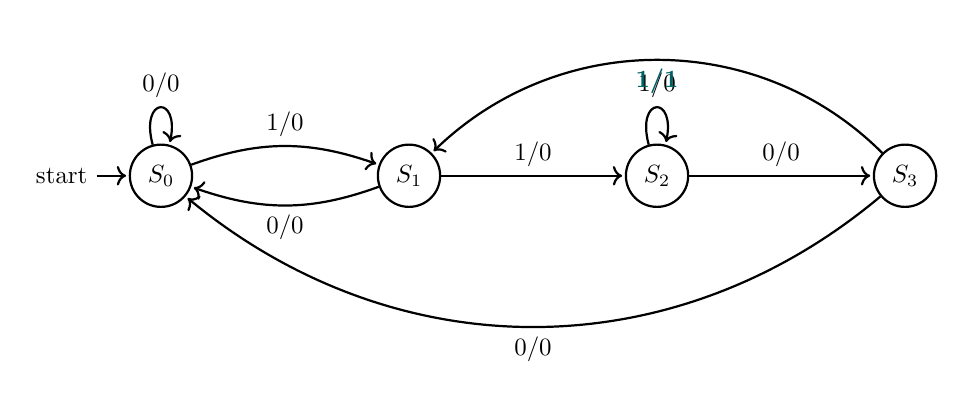
\begin{tikzpicture}[shorten >=1pt, node distance=3.5cm, on grid, auto, thick, scale=0.9, transform shape]
    \node[state, initial] (S0) {$S_0$};
    \node[state] (S1) [right=of S0] {$S_1$};
    \node[state] (S2) [right=of S1] {$S_2$};
    \node[state] (S3) [right=of S2] {$S_3$};

    \path[->]
    (S0) edge [loop above] node {0/0} (S0)
         edge [bend left=20] node {1/0} (S1)
    (S1) edge [bend left=20] node {0/0} (S0)
         edge node {1/0} (S2)
    (S2) edge node {0/0} (S3)
         edge [loop above] node {1/0} (S2)
    (S3) edge [bend left=40] node {0/0} (S0)
         edge [bend right=45] node[text=cF, font=\bfseries] {1/1} (S1); % Overlap transition
\end{tikzpicture}
\end{center}

\vspace{0.5cm}
\subsubsection*{2. Excitation Table for SR Flip-Flops}

The excitation logic for an SR Flip-Flop based on present ($Q$) and next ($Q^+$) states is:
\begin{center}
$0 \rightarrow 0 \implies S=0, R=d \quad|\quad 0 \rightarrow 1 \implies S=1, R=0 \quad|\quad 1 \rightarrow 0 \implies S=0, R=1 \quad|\quad 1 \rightarrow 1 \implies S=d, R=0$
\end{center}

We expand the state diagram into the Transition and Excitation Table:

\begin{center}
\begin{tabular}{ccc@{\hskip 0.3in}cc@{\hskip 0.3in}cc@{\hskip 0.3in}cc@{\hskip 0.3in}c}
\toprule
\multicolumn{2}{c}{\textbf{Present State}} & \textbf{Input} & \multicolumn{2}{c}{\textbf{Next State}} & \multicolumn{2}{c}{\textbf{FF1 Inputs}} & \multicolumn{2}{c}{\textbf{FF0 Inputs}} & \textbf{Output} \\
$Q_1$ & $Q_0$ & $X$ & $Q_1^+$ & $Q_0^+$ & $S_1$ & $R_1$ & $S_0$ & $R_0$ & $Y$ \\
\midrule
0 & 0 & 0 & 0 & 0 & 0 & d & 0 & d & 0 \\
0 & 0 & 1 & 0 & 1 & 0 & d & 1 & 0 & 0 \\
0 & 1 & 0 & 0 & 0 & 0 & d & 0 & 1 & 0 \\
0 & 1 & 1 & 1 & 0 & 1 & 0 & 0 & 1 & 0 \\
1 & 0 & 0 & 1 & 1 & d & 0 & 1 & 0 & 0 \\
1 & 0 & 1 & 1 & 0 & d & 0 & 0 & d & 0 \\
1 & 1 & 0 & 0 & 0 & 0 & 1 & 0 & 1 & 0 \\
1 & 1 & 1 & 0 & 1 & 0 & 1 & d & 0 & 1 \\
\bottomrule
\end{tabular}
\end{center}

\vspace{0.5cm}
\subsubsection*{3. Karnaugh Maps and Boolean Equations}

We derive the simplified Boolean expressions for $S_1, R_1, S_0, R_0$ and Output $Y$.

\vspace{0.3cm}
\noindent
\begin{minipage}{0.48\textwidth}
\textbf{K-Map for $S_1$:}
\begin{center}
\begin{karnaugh-map}[4][2][1][$Q_0X$][$Q_1$]
    \minterms{3}
    \indeterminants{4,5}
    \autoterms[0]
    \implicant{3}{3}
\end{karnaugh-map}
\end{center}
\begin{align*}
    S_1 &= \bar{Q}_1 Q_0 X
\end{align*}
\end{minipage}
\hfill
\begin{minipage}{0.48\textwidth}
\textbf{K-Map for $R_1$:}
\begin{center}
\begin{karnaugh-map}[4][2][1][$Q_0X$][$Q_1$]
    \minterms{6,7}
    \indeterminants{0,1,2}
    \autoterms[0]
    \implicant{7}{6}
\end{karnaugh-map}
\end{center}
\begin{align*}
    R_1 &= Q_1 Q_0
\end{align*}
\end{minipage}

\vspace{0.5cm}
\noindent
\begin{minipage}{0.48\textwidth}
\textbf{K-Map for $S_0$:}
\begin{center}
\begin{karnaugh-map}[4][2][1][$Q_0X$][$Q_1$]
    \minterms{1,4}
    \indeterminants{7}
    \autoterms[0]
    \implicant{1}{1}
    \implicant{4}{4}
\end{karnaugh-map}
\end{center}
\begin{align*}
    S_0 &= \bar{Q}_1 \bar{Q}_0 X + Q_1 \bar{Q}_0 \bar{X} \\
        &= \bar{Q}_0 (Q_1 \oplus X) 
\end{align*}
\end{minipage}
\hfill
\begin{minipage}{0.48\textwidth}
\textbf{K-Map for $R_0$:}
\begin{center}
\begin{karnaugh-map}[4][2][1][$Q_0X$][$Q_1$]
    \minterms{2,3,6}
    \indeterminants{0,5}
    \autoterms[0]
    \implicant{3}{2}
    \implicant{2}{6}
\end{karnaugh-map}
\end{center}
\begin{align*}
    R_0 &= \bar{Q}_1 Q_0 + Q_0 \bar{X} \\
        &= Q_0 (\bar{Q}_1 + \bar{X}) = Q_0 \cdot \overline{(Q_1 X)}
\end{align*}
\end{minipage}

\vspace{0.3cm}
\noindent
\textbf{Output $Y$:}
Since $Y = 1$ only for minterm $7$ ($Q_1=1, Q_0=1, X=1$), the expression is:
\begin{align*}
    Y &= Q_1 Q_0 X
\end{align*}

\vspace{0.5cm}
\subsubsection*{4. Logic Circuit Implementation}

To maintain clarity, standard combinational logic gates are used alongside modular labels for the Flip-Flop outputs to prevent heavily crossed wires. 

\begin{center}
\begin{circuitikz}[scale=0.95, transform shape, font=\sffamily]
    % Draw SR Flip-Flop 1
    \node[draw, thick, minimum width=1.5cm, minimum height=2.2cm, rounded corners=2pt] (FF1) at (7, 1) {};
    \node at (FF1) {\large $\text{FF}_1$};
    \node[right, font=\footnotesize] at (FF1.west |- 7, 1.6) {$S$};
    \node[right, font=\footnotesize] at (FF1.west |- 7, 1) {CLK};
    \node[right, font=\footnotesize] at (FF1.west |- 7, 0.4) {$R$};
    \node[left, font=\footnotesize] at (FF1.east |- 7, 1.6) {$Q_1$};
    \node[left, font=\footnotesize] at (FF1.east |- 7, 0.4) {$\bar{Q}_1$};
    
    \coordinate (S1) at (FF1.west |- 7, 1.6);
    \coordinate (C1) at (FF1.west |- 7, 1);
    \coordinate (R1) at (FF1.west |- 7, 0.4);
    \coordinate (Q1) at (FF1.east |- 7, 1.6);
    \coordinate (Q1bar) at (FF1.east |- 7, 0.4);
    
    % Draw SR Flip-Flop 0
    \node[draw, thick, minimum width=1.5cm, minimum height=2.2cm, rounded corners=2pt] (FF0) at (7, -3.5) {};
    \node at (FF0) {\large $\text{FF}_0$};
    \node[right, font=\footnotesize] at (FF0.west |- 7, -2.9) {$S$};
    \node[right, font=\footnotesize] at (FF0.west |- 7, -3.5) {CLK};
    \node[right, font=\footnotesize] at (FF0.west |- 7, -4.1) {$R$};
    \node[left, font=\footnotesize] at (FF0.east |- 7, -2.9) {$Q_0$};
    \node[left, font=\footnotesize] at (FF0.east |- 7, -4.1) {$\bar{Q}_0$};
    
    \coordinate (S0) at (FF0.west |- 7, -2.9);
    \coordinate (C0) at (FF0.west |- 7, -3.5);
    \coordinate (R0) at (FF0.west |- 7, -4.1);
    \coordinate (Q0) at (FF0.east |- 7, -2.9);
    \coordinate (Q0bar) at (FF0.east |- 7, -4.1);

    % Outputs Tags
    \draw (Q1) -- ++(0.5,0) node[right, font=\scriptsize] {$Q_1$};
    \draw (Q1bar) -- ++(0.5,0) node[right, font=\scriptsize] {$\bar{Q}_1$};
    \draw (Q0) -- ++(0.5,0) node[right, font=\scriptsize] {$Q_0$};
    \draw (Q0bar) -- ++(0.5,0) node[right, font=\scriptsize] {$\bar{Q}_0$};
    
    % S1 = Q1' Q0 X
    \node[and port, number inputs=3] (ANDS1) at (4, 2) {};
    \node[left, font=\scriptsize] at (ANDS1.in 1) {$\bar{Q}_1$};
    \node[left, font=\scriptsize] at (ANDS1.in 2) {$Q_0$};
    \node[left, font=\scriptsize] at (ANDS1.in 3) {$X$};
    \draw (ANDS1.out) |- (S1);

    % R1 = Q1 Q0
    \node[and port] (ANDR1) at (4, 0.4) {};
    \node[left, font=\scriptsize] at (ANDR1.in 1) {$Q_1$};
    \node[left, font=\scriptsize] at (ANDR1.in 2) {$Q_0$};
    \draw (ANDR1.out) -- (R1);

    % S0 = Q0' (Q1 XOR X)
    \node[xor port] (XORS0) at (1, -2.5) {};
    \node[left, font=\scriptsize] at (XORS0.in 1) {$Q_1$};
    \node[left, font=\scriptsize] at (XORS0.in 2) {$X$};
    
    \node[and port] (ANDS0) at (4, -2.9) {};
    \node[left, font=\scriptsize] at (ANDS0.in 1) {$\bar{Q}_0$};
    \draw (XORS0.out) |- (ANDS0.in 2);
    \draw (ANDS0.out) -- (S0);

    % R0 = Q0 (Q1 X)'  using NAND -> AND
    \node[nand port] (NANDR0) at (1, -4.5) {};
    \node[left, font=\scriptsize] at (NANDR0.in 1) {$Q_1$};
    \node[left, font=\scriptsize] at (NANDR0.in 2) {$X$};
    
    \node[and port] (ANDR0) at (4, -4.1) {};
    \draw (NANDR0.out) |- (ANDR0.in 2);
    \node[left, font=\scriptsize] at (ANDR0.in 1) {$Q_0$};
    \draw (ANDR0.out) -- (R0);

    % Y = Q1 Q0 X
    \node[and port, number inputs=3] (ANDY) at (11, -1.25) {};
    \node[left, font=\scriptsize] at (ANDY.in 1) {$Q_1$};
    \node[left, font=\scriptsize] at (ANDY.in 2) {$Q_0$};
    \node[left, font=\scriptsize] at (ANDY.in 3) {$X$};
    \draw (ANDY.out) -- ++(0.5,0) node[right, font=\bfseries] {$Y$ (Output)};

    % Clock network
    \node[left, font=\bfseries] (CLK) at (5.5, -1.25) {Clock};
    \draw (CLK) |- (C1);
    \draw (CLK) |- (C0);

\end{circuitikz}
\end{center}

\end{tcolorbox}

\item Design a clocked sequential circuit that recognizes the input sequence \textbf{1010} (including overlap) such that for input $x = 01010100011010010100$ the output is $z = 00001010000001000010$. Design the circuit using T Flip-Flops and basic gates.
\mk{20} \yr{CSE 205 | L-2/T-1 | 2016--17}

\begin{tcolorbox}[enhanced,breakable,ansbox,colback=cF!4,colframe=cF,boxrule=0.8pt,arc=5pt,title={\textbf{Answer}},fonttitle=\bfseries\color{white},colbacktitle=cF]

To detect the sequence \textbf{1010} with \textbf{overlap allowed}, we will design a \textbf{Mealy Machine} since the output $z$ depends on both the present state and the current input $x$. A Mealy machine allows sequence detection to be signaled concurrently with the final bit's arrival.

\vspace{0.5cm}
\subsubsection*{1. State Definitions and State Diagram (FSM)}

We define four states to track the longest successful prefix of the target sequence `1010`:
\begin{itemize}
    \item \textbf{$S_0$ (Reset):} Initial state, no valid prefix. (Encoding: $Q_1Q_0 = 00$)
    \item \textbf{$S_1$:} Prefix \textbf{`1'} detected. (Encoding: $Q_1Q_0 = 01$)
    \item \textbf{$S_2$:} Prefix \textbf{`10'} detected. (Encoding: $Q_1Q_0 = 10$)
    \item \textbf{$S_3$:} Prefix \textbf{`101'} detected. (Encoding: $Q_1Q_0 = 11$)
\end{itemize}

\textbf{Handling the overlap:} If the machine is in state $S_3$ (has prefix `101`) and receives an input $x = 0$, the full sequence `1010` is detected, so output $z = 1$. The last two bits of this completed sequence (`10`) concurrently form a valid prefix for the \textit{next} possible sequence. Therefore, the next state is $S_2$. 

\begin{center}
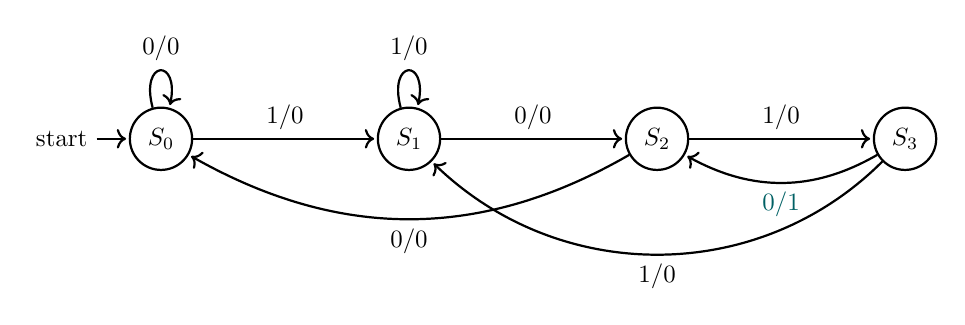
\begin{tikzpicture}[shorten >=1pt, node distance=3.5cm, on grid, auto, thick, scale=0.9, transform shape]
    \node[state, initial] (S0) {$S_0$};
    \node[state] (S1) [right=of S0] {$S_1$};
    \node[state] (S2) [right=of S1] {$S_2$};
    \node[state] (S3) [right=of S2] {$S_3$};

    \path[->]
    (S0) edge [loop above] node {$0/0$} (S0)
         edge node {$1/0$} (S1)
    (S1) edge node {$0/0$} (S2)
         edge [loop above] node {$1/0$} (S1)
    (S2) edge [bend left=30] node {$0/0$} (S0)
         edge node {$1/0$} (S3)
    (S3) edge [bend left=30] node[text=cF, font=\bfseries] {$0/1$} (S2) % Overlap and output
         edge [bend left=45] node {$1/0$} (S1);
\end{tikzpicture}
\end{center}

\vspace{0.5cm}
\subsubsection*{2. Excitation Table for T Flip-Flops}

The state transition logic is expanded using the T Flip-Flop excitation rule: $T = Q \oplus Q^+$.

\begin{center}
\begin{tabular}{ccc@{\hskip 0.4in}cc@{\hskip 0.4in}cc@{\hskip 0.4in}c}
\toprule
\multicolumn{2}{c}{\textbf{Present State}} & \textbf{Input} & \multicolumn{2}{c}{\textbf{Next State}} & \multicolumn{2}{c}{\textbf{T-FF Inputs}} & \textbf{Output} \\
$Q_1$ & $Q_0$ & $x$ & $Q_1^+$ & $Q_0^+$ & $T_1$ & $T_0$ & $z$ \\
\midrule
0 & 0 & 0 & 0 & 0 & 0 & 0 & 0 \\
0 & 0 & 1 & 0 & 1 & 0 & 1 & 0 \\
0 & 1 & 0 & 1 & 0 & 1 & 1 & 0 \\
0 & 1 & 1 & 0 & 1 & 0 & 0 & 0 \\
1 & 0 & 0 & 0 & 0 & 1 & 0 & 0 \\
1 & 0 & 1 & 1 & 1 & 0 & 1 & 0 \\
1 & 1 & 0 & 1 & 0 & 0 & 1 & 1 \\
1 & 1 & 1 & 0 & 1 & 1 & 0 & 0 \\
\bottomrule
\end{tabular}
\end{center}

\vspace{0.5cm}
\subsubsection*{3. Karnaugh Maps and Boolean Equations}

We derive the simplified Boolean expressions for $T_1$, $T_0$, and $z$.

\vspace{0.3cm}
\noindent
\begin{minipage}{0.48\textwidth}
\textbf{K-Map for $T_1$:}
\begin{center}
\begin{karnaugh-map}[4][2][1][$Q_0x$][$Q_1$]
    \minterms{2,4,7}
    \autoterms[0]
    \implicant{2}{2}
    \implicant{4}{4}
    \implicant{7}{7}
\end{karnaugh-map}
\end{center}
\begin{align*}
    T_1 &= \bar{Q}_1 Q_0 \bar{x} + Q_1 \bar{Q}_0 \bar{x} + Q_1 Q_0 x \\
        &= (Q_1 \oplus Q_0)\bar{x} + Q_1 Q_0 x
\end{align*}
\end{minipage}
\hfill
\begin{minipage}{0.48\textwidth}
\textbf{K-Map for $T_0$:}
\begin{center}
\begin{karnaugh-map}[4][2][1][$Q_0x$][$Q_1$]
    \minterms{1,2,5,6}
    \autoterms[0]
    \implicant{1}{5}
    \implicant{2}{6}
\end{karnaugh-map}
\end{center}
\begin{align*}
    T_0 &= \bar{Q}_0 x + Q_0 \bar{x} \\
        &= Q_0 \oplus x
\end{align*}
\end{minipage}

\vspace{0.5cm}
\noindent
\textbf{Output $z$ K-Map \& Equation:}
The output $z$ is active only at minterm 6 ($Q_1=1, Q_0=1, x=0$).
\begin{align*}
    z &= Q_1 Q_0 \bar{x}
\end{align*}

\vspace{0.5cm}
\subsubsection*{4. Logic Circuit Implementation}

To maintain clarity and a highly readable schematic, modular node labeling is utilized for state feedback connections, avoiding heavily crossed wiring.

\begin{center}
\begin{circuitikz}[scale=0.9, transform shape, font=\sffamily]
    % T Flip-Flop 1
    \node[draw, thick, minimum width=1.5cm, minimum height=2.2cm, rounded corners=2pt] (FF1) at (9, 0) {};
    \node at (FF1) {\large $\text{FF}_1$};
    \node[right, font=\footnotesize] at (FF1.west |- 9, 0.6) {$T$};
    \node[right, font=\footnotesize] at (FF1.west |- 9, -0.6) {CLK};
    \node[left, font=\footnotesize] at (FF1.east |- 9, 0.6) {$Q_1$};
    \node[left, font=\footnotesize] at (FF1.east |- 9, -0.6) {$\bar{Q}_1$};
    
    \coordinate (T1) at (FF1.west |- 9, 0.6);
    \coordinate (C1) at (FF1.west |- 9, -0.6);
    \coordinate (Q1) at (FF1.east |- 9, 0.6);
    
    % T Flip-Flop 0
    \node[draw, thick, minimum width=1.5cm, minimum height=2.2cm, rounded corners=2pt] (FF0) at (9, -4) {};
    \node at (FF0) {\large $\text{FF}_0$};
    \node[right, font=\footnotesize] at (FF0.west |- 9, -3.4) {$T$};
    \node[right, font=\footnotesize] at (FF0.west |- 9, -4.6) {CLK};
    \node[left, font=\footnotesize] at (FF0.east |- 9, -3.4) {$Q_0$};
    \node[left, font=\footnotesize] at (FF0.east |- 9, -4.6) {$\bar{Q}_0$};
    
    \coordinate (T0) at (FF0.west |- 9, -3.4);
    \coordinate (C0) at (FF0.west |- 9, -4.6);
    \coordinate (Q0) at (FF0.east |- 9, -3.4);
    
    % Draw Output Tags for FF Q's
    \draw (Q1) -- ++(0.5,0) node[right, font=\scriptsize] {$Q_1$};
    \draw (Q0) -- ++(0.5,0) node[right, font=\scriptsize] {$Q_0$};

    % Gates for T1 = (Q1 XOR Q0)x' + Q1 Q0 x
    \node[xor port] (XOR1) at (2, 1.5) {};
    \node[left, font=\scriptsize] at (XOR1.in 1) {$Q_1$};
    \node[left, font=\scriptsize] at (XOR1.in 2) {$Q_0$};
    
    \node[not port, scale=0.7] (NOTx) at (2, 0.5) {};
    \node[left, font=\scriptsize] at (NOTx.in) {$x$};
    
    \node[and port] (AND1a) at (4.5, 1) {};
    \draw (XOR1.out) |- (AND1a.in 1);
    \draw (NOTx.out) |- (AND1a.in 2);
    
    \node[and port, number inputs=3] (AND1b) at (4.5, -1) {};
    \node[left, font=\scriptsize] at (AND1b.in 1) {$Q_1$};
    \node[left, font=\scriptsize] at (AND1b.in 2) {$Q_0$};
    \node[left, font=\scriptsize] at (AND1b.in 3) {$x$};
    
    \node[or port] (OR1) at (7, 0.6) {};
    \draw (AND1a.out) |- (OR1.in 1);
    \draw (AND1b.out) |- (OR1.in 2);
    \draw (OR1.out) -- (T1);
    
    % Gates for T0 = Q0 XOR x
    \node[xor port] (XOR0) at (4.5, -3.4) {};
    \node[left, font=\scriptsize] at (XOR0.in 1) {$Q_0$};
    \node[left, font=\scriptsize] at (XOR0.in 2) {$x$};
    \draw (XOR0.out) -- (T0);

    % Gate for z = Q1 Q0 x'
    \node[and port, number inputs=3] (ANDz) at (13, -2) {};
    \node[left, font=\scriptsize] at (ANDz.in 1) {$Q_1$};
    \node[left, font=\scriptsize] at (ANDz.in 2) {$Q_0$};
    \node[left, font=\scriptsize] at (ANDz.in 3) {$\bar{x}$};
    \draw (ANDz.out) -- ++(0.5,0) node[right, font=\bfseries] {$z$ (Output)};

    % Clock Network
    \node[left, font=\bfseries] (CLK) at (7, -2.5) {Clock};
    \draw (CLK) |- (C1);
    \draw (CLK) |- (C0);

\end{circuitikz}
\end{center}

\end{tcolorbox}

\item Draw the state diagram in Moore model of a synchronous sequential circuit that results in an output of 1 whenever the sequence $10011$ occurs. The circuit is required to recognize overlapping sequences.
\mk{8} \yr{CSE 205 | L-2/T-1 | 2012--13}

\begin{tcolorbox}[enhanced,breakable,ansbox,colback=cF!4,colframe=cF,boxrule=0.8pt,arc=5pt,title={\textbf{Answer}},fonttitle=\bfseries\color{white},colbacktitle=cF]

To design a \textbf{Moore machine} that detects the sequence \textbf{10011} with \textbf{overlapping allowed}, we associate the output directly with the states. A Moore machine requires one more state than the number of bits in the target sequence to represent the initial state and the progression through the sequence.

\vspace{0.5cm}
\subsubsection*{1. State Definitions}
Let us define the states based on the longest matching prefix of the sequence \textbf{10011} that has been detected so far. In a Moore machine, the format of each state is represented as $S_i / Z$, where $Z$ is the output.

\begin{itemize}
    \item \textbf{$S_0$}: Initial state, no valid prefix detected. Output = $0$.
    \item \textbf{$S_1$}: Prefix \textbf{`1'} detected. Output = $0$.
    \item \textbf{$S_2$}: Prefix \textbf{`10'} detected. Output = $0$.
    \item \textbf{$S_3$}: Prefix \textbf{`100'} detected. Output = $0$.
    \item \textbf{$S_4$}: Prefix \textbf{`1001'} detected. Output = $0$.
    \item \textbf{$S_5$}: Full sequence \textbf{`10011'} detected. Output = \textbf{\textcolor{cF}{1}}.
\end{itemize}

\vspace{0.5cm}
\subsubsection*{2. Overlap Handling and Transition Logic}
Since the machine allows overlapping, the final bits of one sequence can serve as the beginning of the next sequence. We analyze transitions from the final state $S_5$ (which has just processed \textbf{`10011'}):
\begin{itemize}
    \item If the next input is \textbf{0}: The continuous sequence is `10011` $\rightarrow$ `0`. The longest valid suffix that forms a new prefix is \textbf{`10'} (from `...1001\textbf{10}`). This matches the condition for state \textbf{$S_2$}.
    \item If the next input is \textbf{1}: The continuous sequence is `10011` $\rightarrow$ `1`. The longest valid suffix that forms a new prefix is \textbf{`1'} (from `...10011\textbf{1}`). This matches the condition for state \textbf{$S_1$}.
\end{itemize}
Similar suffix-prefix matching logic is applied to breakages in the sequence at any intermediate state (e.g., from $S_3$ receiving a `0`, the suffix is `1000`, which contains no valid prefix, sending it back to $S_0$).

\vspace{0.5cm}
\subsubsection*{3. State Transition Table}

\begin{center}
\begin{tabular}{cccc}
\toprule
\textbf{Present State} & \multicolumn{2}{c}{\textbf{Next State}} & \textbf{Output ($Z$)} \\
& \textbf{Input $X = 0$} & \textbf{Input $X = 1$} & \\
\midrule
$S_0$ & $S_0$ & $S_1$ & 0 \\
$S_1$ & $S_2$ & $S_1$ & 0 \\
$S_2$ & $S_3$ & $S_1$ & 0 \\
$S_3$ & $S_0$ & $S_4$ & 0 \\
$S_4$ & $S_2$ & $S_5$ & 0 \\
$S_5$ & $S_2$ & $S_1$ & \textbf{\textcolor{cF}{1}} \\
\bottomrule
\end{tabular}
\end{center}

\vspace{0.5cm}
\subsubsection*{4. State Diagram}

\begin{center}
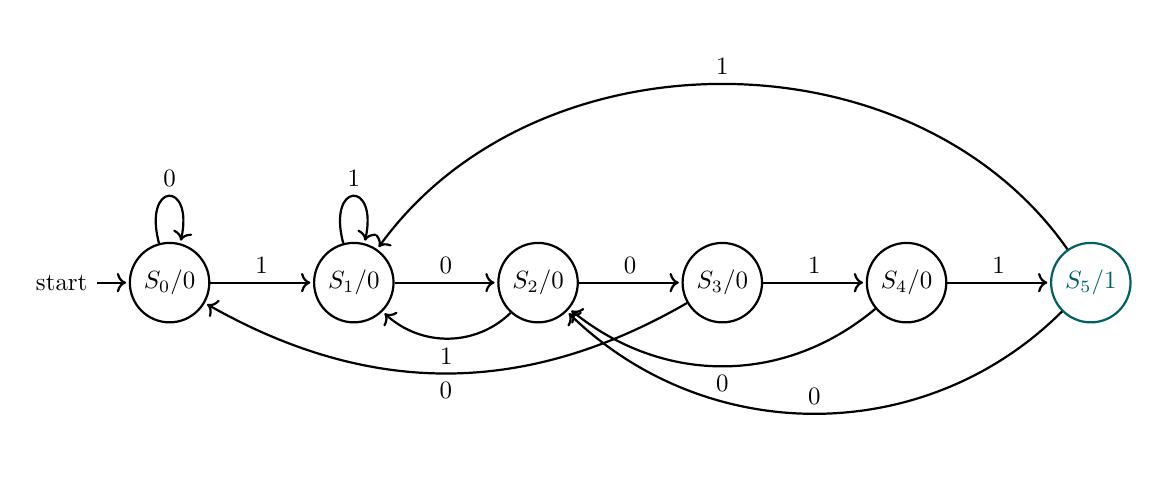
\begin{tikzpicture}[shorten >=1pt, node distance=2.6cm, on grid, auto, thick, scale=0.9, transform shape]
    % State Nodes
    \node[state, initial] (S0) {$S_0/0$};
    \node[state] (S1) [right=of S0] {$S_1/0$};
    \node[state] (S2) [right=of S1] {$S_2/0$};
    \node[state] (S3) [right=of S2] {$S_3/0$};
    \node[state] (S4) [right=of S3] {$S_4/0$};
    \node[state, text=cF, draw=cF] (S5) [right=of S4] {$S_5/1$};

    % Main forward path (detecting 10011)
    \path[->] (S0) edge node {1} (S1);
    \path[->] (S1) edge node {0} (S2);
    \path[->] (S2) edge node {0} (S3);
    \path[->] (S3) edge node {1} (S4);
    \path[->] (S4) edge node {1} (S5);

    % Reset/Self loops and broken paths
    \path[->] (S0) edge [loop above] node {0} (S0);
    \path[->] (S1) edge [loop above] node {1} (S1);
    
    % From S2 (prefix 10)
    \path[->] (S2) edge [bend left=45] node {1} (S1); 
    
    % From S3 (prefix 100)
    \path[->] (S3) edge [bend left=30] node {0} (S0);
    
    % From S4 (prefix 1001)
    \path[->] (S4) edge [bend left=40] node {0} (S2);
    
    % Overlap handling from S5 (sequence 10011 found)
    \path[->] (S5) edge [bend left=45] node[above] {0} (S2);
    \path[->] (S5) edge [bend right=55] node[above] {1} (S1);
    
\end{tikzpicture}
\end{center}

\end{tcolorbox}

\item Design a sequential circuit that detects a sequence of three or more consecutive 1s in a string of bits coming through an input line. Use D flip-flops. The design must include the following:
\begin{enumerate}
  \item State diagram
  \item State table
  \item Simplified logic equations
  \item Logic 
\end{enumerate}
\mk{15} \yr{CSE 205 | L-2/T-1 | 2011--12}

\begin{tcolorbox}[enhanced,breakable,ansbox,colback=cF!4,colframe=cF,boxrule=0.8pt,arc=5pt,title={\textbf{Answer}},fonttitle=\bfseries\color{white},colbacktitle=cF]

To design a sequential circuit that detects three or more consecutive \textbf{1}s, we will use a \textbf{Moore Machine} model, where the output depends solely on the current state.

\vspace{0.3cm}
\subsubsection*{1. State Definitions and State Diagram (FSM)}

We define four states to track the number of consecutive \textbf{1}s received from the input $X$:
\begin{itemize}
    \item \textbf{$S_0$ (Reset):} Zero consecutive 1s detected. (Encoding: $Q_1Q_0 = 00$, Output $Y = 0$)
    \item \textbf{$S_1$:} One \textbf{1} detected. (Encoding: $Q_1Q_0 = 01$, Output $Y = 0$)
    \item \textbf{$S_2$:} Two consecutive \textbf{1}s detected. (Encoding: $Q_1Q_0 = 10$, Output $Y = 0$)
    \item \textbf{$S_3$:} Three or more consecutive \textbf{1}s detected. (Encoding: $Q_1Q_0 = 11$, Output $Y = 1$)
\end{itemize}

Any input of \textbf{0} breaks the sequence and returns the machine to the initial state $S_0$.

\begin{center}
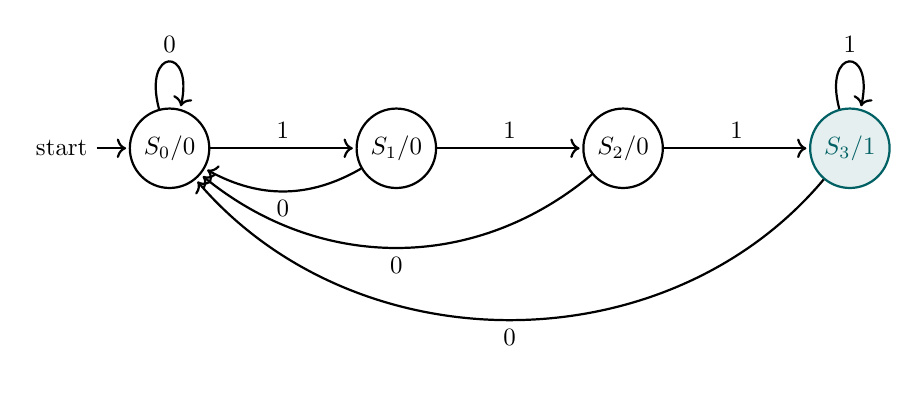
\begin{tikzpicture}[shorten >=1pt, node distance=3.2cm, on grid, auto, thick, scale=0.9, transform shape]
    \node[state, initial] (S0) {$S_0/0$};
    \node[state] (S1) [right=of S0] {$S_1/0$};
    \node[state] (S2) [right=of S1] {$S_2/0$};
    \node[state, text=cF, draw=cF, fill=cF!10] (S3) [right=of S2] {$S_3/1$};

    \path[->]
    (S0) edge [loop above] node {0} (S0)
         edge node {1} (S1)
    (S1) edge [bend left=30] node {0} (S0)
         edge node {1} (S2)
    (S2) edge [bend left=40] node {0} (S0)
         edge node {1} (S3)
    (S3) edge [bend left=50] node {0} (S0)
         edge [loop above] node {1} (S3);
\end{tikzpicture}
\end{center}

\vspace{0.3cm}
\subsubsection*{2. State Table and Excitation Table}

Since we are using D flip-flops, the next state is equal to the D input ($D = Q^+$). We expand the state transitions into a truth table.

\begin{center}
\begin{tabular}{ccc@{\hskip 0.4in}cc@{\hskip 0.4in}cc@{\hskip 0.4in}c}
\toprule
\multicolumn{2}{c}{\textbf{Present State}} & \textbf{Input} & \multicolumn{2}{c}{\textbf{Next State}} & \multicolumn{2}{c}{\textbf{D-FF Inputs}} & \textbf{Output} \\
$Q_1$ & $Q_0$ & $X$ & $Q_1^+$ & $Q_0^+$ & $D_1$ & $D_0$ & $Y$ \\
\midrule
0 & 0 & 0 & 0 & 0 & 0 & 0 & 0 \\
0 & 0 & 1 & 0 & 1 & 0 & 1 & 0 \\
0 & 1 & 0 & 0 & 0 & 0 & 0 & 0 \\
0 & 1 & 1 & 1 & 0 & 1 & 0 & 0 \\
1 & 0 & 0 & 0 & 0 & 0 & 0 & 0 \\
1 & 0 & 1 & 1 & 1 & 1 & 1 & 0 \\
1 & 1 & 0 & 0 & 0 & 0 & 0 & \textbf{\textcolor{cF}{1}} \\
1 & 1 & 1 & 1 & 1 & 1 & 1 & \textbf{\textcolor{cF}{1}} \\
\bottomrule
\end{tabular}
\end{center}

\vspace{0.3cm}
\subsubsection*{3. Karnaugh Maps and Simplified Logic Equations}

We extract the simplified Boolean expressions for $D_1$, $D_0$, and $Y$ based on the minterms from the table.

\vspace{0.2cm}
\noindent
\begin{minipage}{0.48\textwidth}
\textbf{K-Map for $D_1$:}
\begin{center}
\begin{karnaugh-map}[4][2][1][$Q_0X$][$Q_1$]
    \minterms{3,5,7}
    \autoterms[0]
    \implicant{3}{7}
    \implicant{5}{7}
\end{karnaugh-map}
\end{center}
\begin{align*}
    D_1 &= Q_1 X + Q_0 X \\
        &= X (Q_1 + Q_0) \quad \text{(Distributive Law)}
\end{align*}
\end{minipage}
\hfill
\begin{minipage}{0.48\textwidth}
\textbf{K-Map for $D_0$:}
\begin{center}
\begin{karnaugh-map}[4][2][1][$Q_0X$][$Q_1$]
    \minterms{1,5,7}
    \autoterms[0]
    \implicant{1}{5}
    \implicant{5}{7}
\end{karnaugh-map}
\end{center}
\begin{align*}
    D_0 &= Q_1 X + \bar{Q}_0 X \\
        &= X (Q_1 + \bar{Q}_0) \quad \text{(Distributive Law)}
\end{align*}
\end{minipage}

\vspace{0.4cm}
\noindent
\textbf{Output $Y$ Equation:}
The output $Y$ is independent of the current input $X$ (Moore Machine) and is active only in state $S_3$ (where $Q_1 = 1$ and $Q_0 = 1$).
\begin{align*}
    Y &= Q_1 \cdot Q_0
\end{align*}

\vspace{0.3cm}
\subsubsection*{4. Logic Circuit Diagram}

Using basic logic gates (AND, OR) and two D flip-flops, we construct the required sequential circuit.

\begin{center}
\begin{circuitikz}[scale=0.9, transform shape, font=\sffamily]
    
    % D Flip-Flop 1
    \node[draw, thick, minimum width=1.5cm, minimum height=2.2cm, rounded corners=2pt] (FF1) at (9, 1) {};
    \node at (FF1) {\large $\text{FF}_1$};
    \node[right, font=\footnotesize] at (FF1.west |- 9, 1.6) {$D$};
    \node[right, font=\footnotesize] at (FF1.west |- 9, 0.4) {CLK};
    \node[left, font=\footnotesize] at (FF1.east |- 9, 1.6) {$Q_1$};
    \node[left, font=\footnotesize] at (FF1.east |- 9, 0.4) {$\bar{Q}_1$};
    
    \coordinate (D1) at (FF1.west |- 9, 1.6);
    \coordinate (C1) at (FF1.west |- 9, 0.4);
    \coordinate (Q1) at (FF1.east |- 9, 1.6);
    
    % D Flip-Flop 0
    \node[draw, thick, minimum width=1.5cm, minimum height=2.2cm, rounded corners=2pt] (FF0) at (9, -3) {};
    \node at (FF0) {\large $\text{FF}_0$};
    \node[right, font=\footnotesize] at (FF0.west |- 9, -2.4) {$D$};
    \node[right, font=\footnotesize] at (FF0.west |- 9, -3.6) {CLK};
    \node[left, font=\footnotesize] at (FF0.east |- 9, -2.4) {$Q_0$};
    \node[left, font=\footnotesize] at (FF0.east |- 9, -3.6) {$\bar{Q}_0$};
    
    \coordinate (D0) at (FF0.west |- 9, -2.4);
    \coordinate (C0) at (FF0.west |- 9, -3.6);
    \coordinate (Q0) at (FF0.east |- 9, -2.4);
    \coordinate (Q0bar) at (FF0.east |- 9, -3.6);

    % Outputs Tags
    \draw (Q1) -- ++(0.5,0) node[right, font=\scriptsize] {$Q_1$};
    \draw (Q0) -- ++(0.5,0) node[right, font=\scriptsize] {$Q_0$};
    \draw (Q0bar) -- ++(0.5,0) node[right, font=\scriptsize] {$\bar{Q}_0$};

    % Gates for D1 = X (Q1 + Q0)
    \node[or port] (OR1) at (4, 2) {};
    \node[left, font=\scriptsize] at (OR1.in 1) {$Q_1$};
    \node[left, font=\scriptsize] at (OR1.in 2) {$Q_0$};
    
    \node[and port] (AND1) at (6.5, 1.6) {};
    \draw (OR1.out) |- (AND1.in 1);
    \node[left, font=\scriptsize] at (AND1.in 2) {$X$};
    \draw (AND1.out) -- (D1);

    % Gates for D0 = X (Q1 + Q0')
    \node[or port] (OR0) at (4, -2) {};
    \node[left, font=\scriptsize] at (OR0.in 1) {$Q_1$};
    \node[left, font=\scriptsize] at (OR0.in 2) {$\bar{Q}_0$};
    
    \node[and port] (AND0) at (6.5, -2.4) {};
    \draw (OR0.out) |- (AND0.in 1);
    \node[left, font=\scriptsize] at (AND0.in 2) {$X$};
    \draw (AND0.out) -- (D0);

    % Output Y = Q1 Q0
    \node[and port] (ANDY) at (13, -1) {};
    \node[left, font=\scriptsize] at (ANDY.in 1) {$Q_1$};
    \node[left, font=\scriptsize] at (ANDY.in 2) {$Q_0$};
    \draw (ANDY.out) -- ++(0.5,0) node[right, font=\bfseries, text=cF] {$Y$};

    % Clock network
    \node[left, font=\bfseries] (CLK) at (7.5, -1.5) {Clock};
    \draw (CLK) |- (C1);
    \draw (CLK) |- (C0);

\end{circuitikz}
\end{center}

\end{tcolorbox}

\end{enumerate}

%%──────────────────────────────────────────────────────────────────────
\subtopic{cF}{Mealy \& Moore Model Comparison \& Block Diagrams}
\label{sub:s6-mealy-moore}

\begin{enumerate}

\item Draw the block diagram of Mealy and Moore state machines. State the difference between two models with a simple example.
\mk{10} \yr{CSE 205 | L-2/T-1 | 2024--25, 2022--23, 2015--16, 2013--14, 2011--12}


\begin{tcolorbox}[enhanced,breakable,ansbox,colback=cF!4,colframe=cF,boxrule=0.8pt,arc=5pt,title={\textbf{Answer}},fonttitle=\bfseries\color{white},colbacktitle=cF]

\subsubsection*{1. Block Diagrams of Mealy and Moore Machines}

The fundamental difference between the two state machine models lies in their output logic. In a \textbf{Mealy machine}, the outputs are a function of both the present state and the current inputs. In a \textbf{Moore machine}, the outputs are a function of the present state only.

\vspace{0.5cm}
\begin{center}
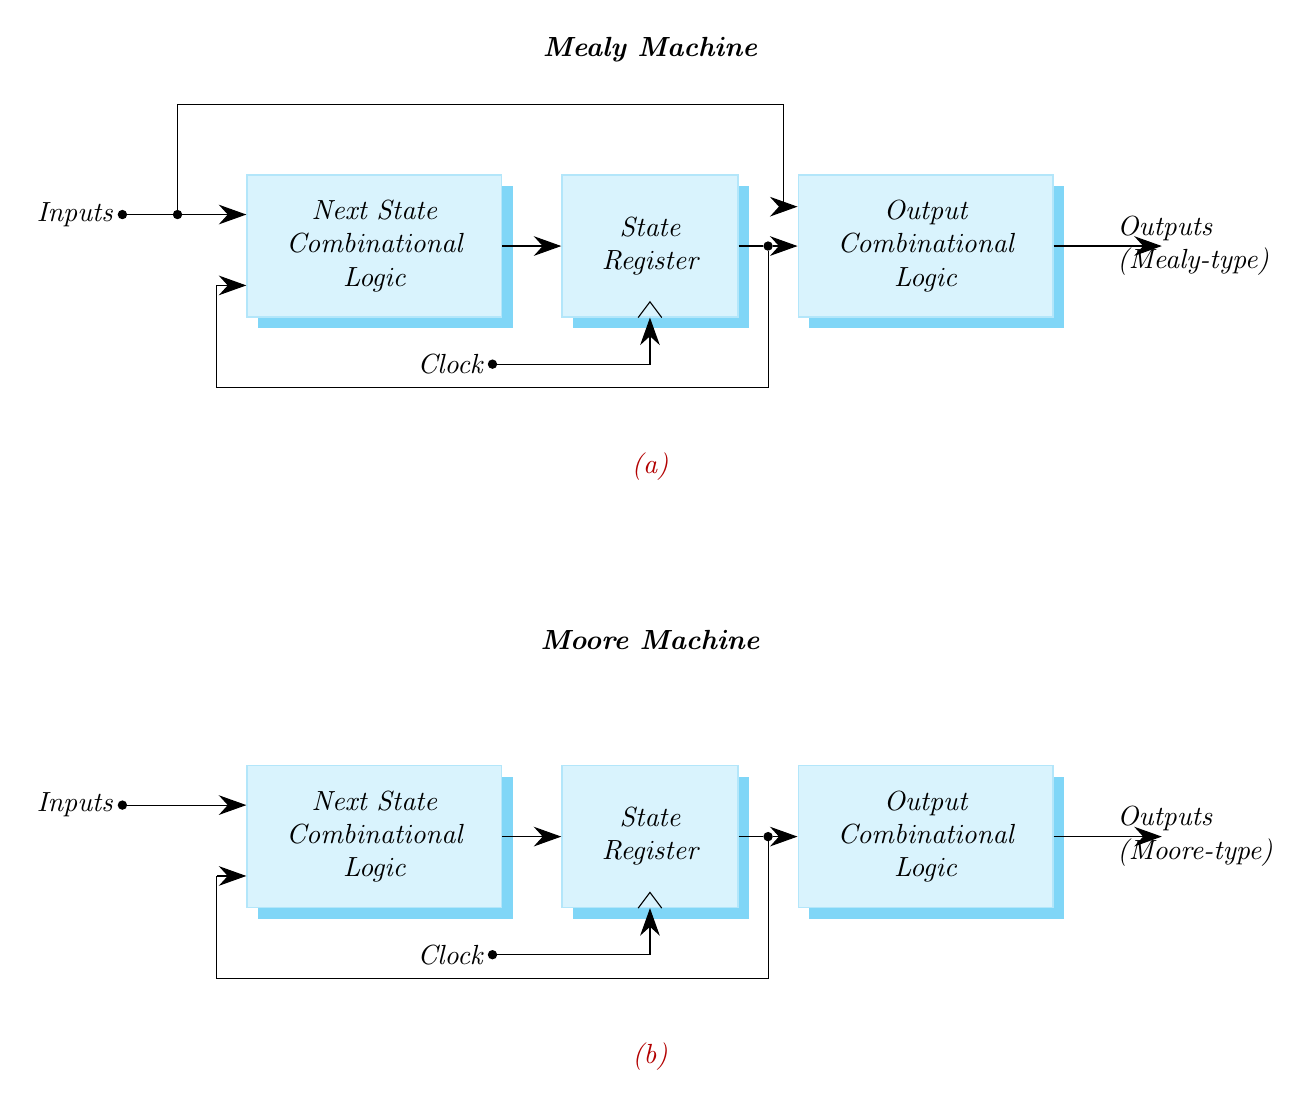
\begin{tikzpicture}[
    >={Stealth[length=3.5mm, width=2.5mm]}, % Arrow head boro and thick kora hoyeche
    font=\itshape,
    block/.style={
        rectangle,
        draw=cyan!30,
        line width=0.5pt,
        fill=cyan!15,
        text width=3cm,
        align=center,
        minimum height=1.8cm,
        % Solid cyan drop shadow matching the textbook style
        drop shadow={shadow xshift=4pt, shadow yshift=-4pt, fill=cyan!50, opacity=1}
    },
    regblock/.style={
        block,
        text width=2cm
    },
    dot/.style={
        circle,
        fill=black,
        inner sep=1.2pt,
        outer sep=0pt
    }
]

    % =======================================================
    % (a) MEALY MACHINE 
    % =======================================================
    \node (titleA) at (3.5, 2.5) {\textbf{\textit{Mealy Machine}}};

    % Main Logic Blocks
    \node[block] (nextA) at (0, 0) {Next State\\Combinational\\Logic};
    \node[regblock] (regA) at (3.5, 0) {State\\Register};
    \node[block] (outA) at (7, 0) {Output\\Combinational\\Logic};

    % Inputs & Dots
    \node[dot] (termInA) at (-3.2, 0.4) {};
    \node[left] at (termInA) {Inputs};
    \node[dot] (inDotA) at (-2.5, 0.4) {};
    \node[dot] (midDotA) at (5.0, 0) {};

    % Output Coordinate
    \coordinate (outpA) at (10, 0);

    % Main Forward Paths
    \draw[-] (termInA) -- (inDotA);
    \draw[->] (inDotA) -- ([yshift=0.4cm]nextA.west);
    \draw[->] (nextA) -- (regA);
    \draw[-] (regA) -- (midDotA);
    \draw[->] (midDotA) -- (outA);
    \draw[->] (outA) -- node[right, align=left] {Outputs\\(Mealy-type)} (outpA);

    % Feedforward Path (Bypasses state register)
    \coordinate (ffUpA) at (-2.5, 1.8);
    \coordinate (ffRightA) at (5.2, 1.8);
    \coordinate (ffDownA) at (5.2, 0.5);
    \draw[-] (inDotA) -- (ffUpA) -- (ffRightA) -- (ffDownA);
    \draw[->] (ffDownA) -- ([yshift=0.5cm]outA.west);

    % Feedback Path (Current state to next state logic)
    \coordinate (fbDownA) at (5.0, -1.8);
    \coordinate (fbLeftA) at (-2.0, -1.8);
    \coordinate (fbUpA) at (-2.0, -0.5);
    \draw[-] (midDotA) -- (fbDownA) -- (fbLeftA) -- (fbUpA);
    \draw[->] (fbUpA) -- ([yshift=-0.5cm]nextA.west);

    % Clock Input
    \node[dot] (termClkA) at (1.5, -1.5) {};
    \node[left] at (termClkA) {Clock};
    \draw[->] (termClkA) -| (regA.south);
    % Clock Edge-Triggered Triangle Symbol
    \draw ([xshift=-1.5mm]regA.south) -- ([yshift=2mm]regA.south) -- ([xshift=1.5mm]regA.south);

    % Diagram Label
    \node[text=red!70!black] at (3.5, -2.8) {(a)};


    % =======================================================
    % (b) MOORE MACHINE
    % =======================================================
    \begin{scope}[yshift=-7.5cm]
        \node (titleB) at (3.5, 2.5) {\textbf{\textit{Moore Machine}}};

        % Main Logic Blocks
        \node[block] (nextB) at (0, 0) {Next State\\Combinational\\Logic};
        \node[regblock] (regB) at (3.5, 0) {State\\Register};
        \node[block] (outB) at (7, 0) {Output\\Combinational\\Logic};

        % Inputs & Dots (Note: No feedforward branch dot needed here)
        \node[dot] (termInB) at (-3.2, 0.4) {};
        \node[left] at (termInB) {Inputs};
        \node[dot] (midDotB) at (5.0, 0) {};

        % Output Coordinate
        \coordinate (outpB) at (10, 0);

        % Main Forward Paths
        \draw[->] (termInB) -- ([yshift=0.4cm]nextB.west);
        \draw[->] (nextB) -- (regB);
        \draw[-] (regB) -- (midDotB);
        \draw[->] (midDotB) -- (outB);
        \draw[->] (outB) -- node[right, align=left] {Outputs\\(Moore-type)} (outpB);

        % Feedback Path
        \coordinate (fbDownB) at (5.0, -1.8);
        \coordinate (fbLeftB) at (-2.0, -1.8);
        \coordinate (fbUpB) at (-2.0, -0.5);
        \draw[-] (midDotB) -- (fbDownB) -- (fbLeftB) -- (fbUpB);
        \draw[->] (fbUpB) -- ([yshift=-0.5cm]nextB.west);

        % Clock Input
        \node[dot] (termClkB) at (1.5, -1.5) {};
        \node[left] at (termClkB) {Clock};
        \draw[->] (termClkB) -| (regB.south);
        % Clock Edge-Triggered Triangle Symbol
        \draw ([xshift=-1.5mm]regB.south) -- ([yshift=2mm]regB.south) -- ([xshift=1.5mm]regB.south);

        % Diagram Label
        \node[text=red!70!black] at (3.5, -2.8) {(b)};
    \end{scope}

\end{tikzpicture}
\end{center}

\vspace{0.5cm}
\subsubsection*{2. Key Differences}

\begin{center}
\renewcommand{\arraystretch}{1.5}
\begin{tabular}{p{3.5cm} p{6cm} p{6cm}}
\toprule
\textbf{Feature} & \textbf{Mealy Machine} & \textbf{Moore Machine} \\
\midrule
\textbf{Output Dependence} & Outputs depend on both the \textbf{present state} and the \textbf{present inputs}. & Outputs depend \textbf{only on the present state}. \\
\textbf{State Count} & Generally requires \textbf{fewer states} to implement the same logic. & Generally requires \textbf{more states}, as distinct outputs require distinct states. \\
\textbf{Output Timing} & Outputs can change asynchronously if an input changes during the clock cycle. & Outputs are strictly synchronous and change only when the state changes. \\
\textbf{Design Complexity} & Output logic is more complex due to the inclusion of input variables. & Output logic is simpler as it relies solely on flip-flop outputs. \\
\bottomrule
\end{tabular}
\end{center}

\vspace{0.3cm}
\subsubsection*{3. Simple Example}

Consider designing a sequence detector that outputs a `1` when the sequence \textbf{"10"} is detected.

\begin{itemize}
    \item \textbf{Mealy Machine Approach:}
    We need only \textbf{2 states}: $S_0$ (Reset/Initial) and $S_1$ (Prefix `1` detected). 
    If the machine is in state $S_1$ and receives a `0`, it transitions back to $S_0$. During this transition, because it sees the required input `0`, it instantly produces the output `1`. The output is attached to the transition: $S_1 \xrightarrow{\text{input}=0 / \text{output}=1} S_0$.
    
    \item \textbf{Moore Machine Approach:}
    We must use \textbf{3 states}: $S_0$ (Reset, Output=0), $S_1$ (Prefix `1` detected, Output=0), and $S_2$ (Sequence `10` detected, Output=1). 
    If the machine is in state $S_1$ and receives a `0`, it must explicitly transition into the new state $S_2$. The output `1` is firmly tied to being inside state $S_2$, regardless of the inputs.
\end{itemize}

\end{tcolorbox}

\item Transform the Mealy machine shown below into a corresponding Moore machine.

\begin{center}
\begin{tabular}{|c|c|c|}
\hline
\multirow{2}{*}{PS} & \multicolumn{2}{c|}{NS, Z} \\ \cline{2-3}
 & $x=0$ & $x=1$ \\ \hline
A & B, 1 & C, 0 \\ \hline
B & C, 1 & D, 0 \\ \hline
C & D, 0 & E, 1 \\ \hline
D & E, 0 & A, 1 \\ \hline
E & A, 1 & B, 1 \\ \hline
\end{tabular}
\end{center}

\mk{6} \yr{CSE 205 | L-2/T-1 | 2023--24}

\begin{tcolorbox}[enhanced,breakable,ansbox,colback=cF!4,colframe=cF,boxrule=0.8pt,arc=5pt,title={\textbf{Answer}},fonttitle=\bfseries\color{white},colbacktitle=cF]

To transform a Mealy machine into a Moore machine, we must associate the outputs with the states rather than the transitions. If a state in the Mealy machine is reached via transitions that produce different outputs, that state must be split into multiple states in the Moore machine, one for each unique output.

\subsubsection*{Step 1: Analyze Incoming Transitions and Outputs}
We examine the given Mealy state table to determine the outputs associated with all incoming transitions for each state.

\begin{itemize}
    \item \textbf{State A:} Reached from D ($x=1$) with output $1$, and from E ($x=0$) with output $1$. 
    \\ $\rightarrow$ Since all incoming transitions have output 1, we create a single Moore state: \textbf{$A_1$} (Output = 1).
    
    \item \textbf{State B:} Reached from A ($x=0$) with output $1$, and from E ($x=1$) with output $1$. 
    \\ $\rightarrow$ All incoming transitions have output 1. We create a single Moore state: \textbf{$B_1$} (Output = 1).
    
    \item \textbf{State C:} Reached from A ($x=1$) with output \textcolor{cF}{\textbf{0}}, and from B ($x=0$) with output \textcolor{cF}{\textbf{1}}. 
    \\ $\rightarrow$ Because it is reached with different outputs, we must \textbf{split State C} into two Moore states: \textbf{$C_0$} (Output = 0) and \textbf{$C_1$} (Output = 1).
    
    \item \textbf{State D:} Reached from B ($x=1$) with output $0$, and from C ($x=0$) with output $0$. 
    \\ $\rightarrow$ All incoming transitions have output 0. We create a single Moore state: \textbf{$D_0$} (Output = 0).
    
    \item \textbf{State E:} Reached from C ($x=1$) with output \textcolor{cF}{\textbf{1}}, and from D ($x=0$) with output \textcolor{cF}{\textbf{0}}. 
    \\ $\rightarrow$ Because it is reached with different outputs, we must \textbf{split State E} into two Moore states: \textbf{$E_0$} (Output = 0) and \textbf{$E_1$} (Output = 1).
\end{itemize}

\subsubsection*{Step 2: Construct the Moore Machine State Table}
We now substitute the newly created states into the next-state entries. For states that were split ($C$ and $E$), both split versions will have identical next-state transition logic, inherited from the original Mealy machine.

\begin{itemize}
    \item \textbf{Transitions for $A_1$:} Originally goes to $B$ (output 1) and $C$ (output 0). In our Moore machine, this maps to $B_1$ and $C_0$.
    \item \textbf{Transitions for $B_1$:} Originally goes to $C$ (output 1) and $D$ (output 0). Maps to $C_1$ and $D_0$.
    \item \textbf{Transitions for $C_0$ and $C_1$:} Originally goes to $D$ (output 0) and $E$ (output 1). Both map to $D_0$ and $E_1$.
    \item \textbf{Transitions for $D_0$:} Originally goes to $E$ (output 0) and $A$ (output 1). Maps to $E_0$ and $A_1$.
    \item \textbf{Transitions for $E_0$ and $E_1$:} Originally goes to $A$ (output 1) and $B$ (output 1). Both map to $A_1$ and $B_1$.
\end{itemize}

\vspace{0.3cm}
\begin{center}
\renewcommand{\arraystretch}{1.3}
\begin{tabular}{cccc}
\toprule
\textbf{Present State} & \multicolumn{2}{c}{\textbf{Next State}} & \textbf{Output ($Z$)} \\
& \textbf{$x=0$} & \textbf{$x=1$} & \\
\midrule
$A_1$ & $B_1$ & $C_0$ & 1 \\
$B_1$ & $C_1$ & $D_0$ & 1 \\
\rowcolor{cF!10} $C_0$ & $D_0$ & $E_1$ & 0 \\
\rowcolor{cF!10} $C_1$ & $D_0$ & $E_1$ & 1 \\
$D_0$ & $E_0$ & $A_1$ & 0 \\
\rowcolor{cF!10} $E_0$ & $A_1$ & $B_1$ & 0 \\
\rowcolor{cF!10} $E_1$ & $A_1$ & $B_1$ & 1 \\
\bottomrule
\end{tabular}
\end{center}

\vspace{0.2cm}
\textit{Note: The states highlighted in color indicate the original Mealy states that required splitting to satisfy the Moore machine requirement of state-dependent outputs.}

\end{tcolorbox}


\item Transform the following Mealy machine into a corresponding Moore machine.

\begin{center}
  \begin{tabular}{|c|c|c|}
\hline
\multirow{2}{*}{PS} & \multicolumn{2}{c|}{NS, Z} \\ \cline{2-3} 
                    & x = 0        & x = 1        \\ \hline
A                   & C, 0         & B, 0         \\ \hline
B                   & A, 1         & D, 0         \\ \hline
C                   & B, 1         & A, 1         \\ \hline
D                   & D, 1         & C, 0         \\ \hline
\end{tabular}
\end{center}

\mk{5} \yr{CSE 205 | L-2/T-1 | 2021--22}

\begin{tcolorbox}[enhanced,breakable,ansbox,colback=cF!4,colframe=cF,boxrule=0.8pt,arc=5pt,title={\textbf{Answer}},fonttitle=\bfseries\color{white},colbacktitle=cF]

To convert a Mealy machine into a Moore machine, we must shift the outputs from the transitions to the states themselves. If a state in the Mealy machine is entered via transitions that produce different outputs, that state must be split into multiple states in the Moore machine—one for each unique output.

\vspace{0.3cm}
\subsubsection*{Step 1: Analyze Incoming Transitions and Outputs}
We list all unique (Next State, Output) pairs from the Mealy state table to determine the required Moore states.

\begin{itemize}
    \item \textbf{State A:} The incoming transitions are from B ($x=0$, output 1) and C ($x=1$, output 1). Since it is only reached with an output of 1, we create a single Moore state: \textbf{$A_1$} (Output = 1).
    
    \item \textbf{State B:} The incoming transitions are from A ($x=1$, output \textcolor{cF}{\textbf{0}}) and C ($x=0$, output \textcolor{cF}{\textbf{1}}). Because it is reached with different outputs, we must \textbf{split State B} into two Moore states: \textbf{$B_0$} (Output = 0) and \textbf{$B_1$} (Output = 1).
    
    \item \textbf{State C:} The incoming transitions are from A ($x=0$, output 0) and D ($x=1$, output 0). Since it is only reached with an output of 0, we create a single Moore state: \textbf{$C_0$} (Output = 0).
    
    \item \textbf{State D:} The incoming transitions are from B ($x=1$, output \textcolor{cF}{\textbf{0}}) and D ($x=0$, output \textcolor{cF}{\textbf{1}}). Because it is reached with different outputs, we must \textbf{split State D} into two Moore states: \textbf{$D_0$} (Output = 0) and \textbf{$D_1$} (Output = 1).
\end{itemize}

\vspace{0.3cm}
\subsubsection*{Step 2: Construct the Moore Machine State Table}
We populate the next-state entries using our newly defined Moore states. When a state is split (like $B$ and $D$), both split versions inherit the exact same transition logic from the original Mealy state.

\begin{itemize}
    \item \textbf{Transitions for $A_1$:} Originally goes to $C$ (output 0) and $B$ (output 0). In the Moore machine, these map to $C_0$ and $B_0$.
    \item \textbf{Transitions for $B_0$ and $B_1$:} Originally goes to $A$ (output 1) and $D$ (output 0). Both map to $A_1$ and $D_0$.
    \item \textbf{Transitions for $C_0$:} Originally goes to $B$ (output 1) and $A$ (output 1). Maps to $B_1$ and $A_1$.
    \item \textbf{Transitions for $D_0$ and $D_1$:} Originally goes to $D$ (output 1) and $C$ (output 0). Both map to $D_1$ and $C_0$.
\end{itemize}

\vspace{0.4cm}
\begin{center}
\renewcommand{\arraystretch}{1.3}
\begin{tabular}{cccc}
\toprule
\textbf{Present State} & \multicolumn{2}{c}{\textbf{Next State}} & \textbf{Output ($Z$)} \\
\cmidrule(lr){2-3}
& \textbf{$x=0$} & \textbf{$x=1$} & \\
\midrule
$A_1$ & $C_0$ & $B_0$ & 1 \\
\textcolor{cF}{\textbf{$B_0$}} & $A_1$ & $D_0$ & 0 \\
\textcolor{cF}{\textbf{$B_1$}} & $A_1$ & $D_0$ & 1 \\
$C_0$ & $B_1$ & $A_1$ & 0 \\
\textcolor{cF}{\textbf{$D_0$}} & $D_1$ & $C_0$ & 0 \\
\textcolor{cF}{\textbf{$D_1$}} & $D_1$ & $C_0$ & 1 \\
\bottomrule
\end{tabular}
\end{center}

\vspace{0.2cm}
\textit{Note: The bold, colored states ($B_0, B_1, D_0, D_1$) highlight where the original Mealy states were split to strictly tie the output to the active state, satisfying the definition of a Moore machine. If $A$ is required to be the initial state and must start with a default output of $0$ at $t=0$, an additional dummy start state $A_0$ would be added; otherwise, this minimal 6-state conversion is exact.}

\end{tcolorbox}

\item Obtain the Mealy equivalent state table for the following Moore machine.

\begin{center}
  \begin{tabular}{|c|c|c|c|}
\hline
\multirow{2}{*}{PS} & \multicolumn{2}{c|}{NS} & \multirow{2}{*}{Z} \\ \cline{2-3}
 & x = 0 & x = 1 & \\ \hline
A & A & B & 0 \\ \hline
B & C & B & 0 \\ \hline
C & C & D & 1 \\ \hline
D & A & D & 0 \\ \hline
\end{tabular}
\end{center}

\mk{7} \yr{CSE 205 | L-2/T-1 | 2018--19}

\begin{tcolorbox}[enhanced,breakable,ansbox,colback=cF!4,colframe=cF,boxrule=0.8pt,arc=5pt,title={\textbf{Answer}},fonttitle=\bfseries\color{white},colbacktitle=cF]

To convert a Moore machine to its equivalent Mealy machine, we must shift the output dependency from the \textbf{states} to the \textbf{transitions}. 

In a Moore machine, the output is a function of the Present State only. In a Mealy machine, the output is a function of both the Present State and the Input. Therefore, the output associated with the \textit{Next State} in the Moore machine becomes the output for the transition leading to that state in the Mealy machine.

\vspace{0.3cm}
\subsubsection*{Step 1: Identify the Outputs for Each State}
From the given Moore machine state table, we can list the outputs strictly associated with each state:
\begin{itemize}
    \item Output of State A: $Z(A) = 0$
    \item Output of State B: $Z(B) = 0$
    \item Output of State C: \textcolor{cF}{\textbf{$Z(C) = 1$}}
    \item Output of State D: $Z(D) = 0$
\end{itemize}

\vspace{0.3cm}
\subsubsection*{Step 2: Map Outputs to the Transitions}
We keep the Next State (NS) mapping identical to the Moore machine. However, for each transition, we assign the output value of the destination state (the Next State).

\begin{itemize}
    \item \textbf{From State A:} 
        \begin{itemize}
            \item If $x = 0$, NS is A. Since $Z(A) = 0$, the transition output is 0.
            \item If $x = 1$, NS is B. Since $Z(B) = 0$, the transition output is 0.
        \end{itemize}
    \item \textbf{From State B:} 
        \begin{itemize}
            \item If $x = 0$, NS is C. Since \textcolor{cF}{\textbf{$Z(C) = 1$}}, the transition output is \textcolor{cF}{\textbf{1}}.
            \item If $x = 1$, NS is B. Since $Z(B) = 0$, the transition output is 0.
        \end{itemize}
    \item \textbf{From State C:} 
        \begin{itemize}
            \item If $x = 0$, NS is C. Since \textcolor{cF}{\textbf{$Z(C) = 1$}}, the transition output is \textcolor{cF}{\textbf{1}}.
            \item If $x = 1$, NS is D. Since $Z(D) = 0$, the transition output is 0.
        \end{itemize}
    \item \textbf{From State D:} 
        \begin{itemize}
            \item If $x = 0$, NS is A. Since $Z(A) = 0$, the transition output is 0.
            \item If $x = 1$, NS is D. Since $Z(D) = 0$, the transition output is 0.
        \end{itemize}
\end{itemize}

\vspace{0.3cm}
\subsubsection*{Step 3: Construct the Equivalent Mealy State Table}

Combining the next states and the newly mapped transition outputs, we obtain the equivalent Mealy machine state table.

\begin{center}
\renewcommand{\arraystretch}{1.4}
\begin{tabular}{ccccc}
\toprule
\textbf{Present State} & \multicolumn{2}{c}{\textbf{Next State, Output (NS, $Z$)}} \\
\cmidrule(lr){2-3}
& \textbf{$x=0$} & \textbf{$x=1$} \\
\midrule
A & A, 0 & B, 0 \\
B & C, \textcolor{cF}{\textbf{1}} & B, 0 \\
C & C, \textcolor{cF}{\textbf{1}} & D, 0 \\
D & A, 0 & D, 0 \\
\bottomrule
\end{tabular}
\end{center}

\vspace{0.2cm}
\textit{Note: The number of states in the converted Mealy machine is equal to the number of states in the original Moore machine. While further state minimization techniques (like an implication chart) could theoretically be applied to the resulting Mealy machine, this direct mapping represents the immediate, equivalent, unminimized Mealy model.}

\end{tcolorbox}

\item Define (i) a Mealy machine and (ii) a Moore machine.
\mk{5} \yr{CSE 205 | L-2/T-1 | 2017--18}

\begin{tcolorbox}[enhanced,breakable,ansbox,colback=cF!4,colframe=cF,boxrule=0.8pt,arc=5pt,title={\textbf{Answer}},fonttitle=\bfseries\color{white},colbacktitle=cF]

In the theory of sequential digital logic, Finite State Machines (FSMs) are broadly categorized into two fundamental models based on how their output logic is structured. 

\vspace{0.3cm}
\subsubsection*{(i) Mealy Machine}
A \textbf{Mealy machine} is a finite state machine whose output values are determined by both its \textcolor{cF}{\textbf{present state}} and its \textcolor{cF}{\textbf{present inputs}}.

\begin{itemize}
    \item \textbf{Mathematical Model:} The output $Z$ at time $t$ is a function of the state $S$ and the input $X$: 
    \begin{align*}
        Z(t) &= f(S(t), X(t))
    \end{align*}
    \item \textbf{Timing and Glitches:} Because the output combinational logic is directly connected to the input lines, any change in the input can cause an immediate, asynchronous change in the output, even between clock edges. This makes Mealy machines susceptible to input glitches.
    \item \textbf{State Efficiency:} They typically require fewer states than Moore machines to implement the same sequential logic function.
\end{itemize}

\vspace{0.4cm}
\subsubsection*{(ii) Moore Machine}
A \textbf{Moore machine} is a finite state machine whose output values are determined \textit{solely} by its \textcolor{cF}{\textbf{present state}}. 

\begin{itemize}
    \item \textbf{Mathematical Model:} The output $Z$ at time $t$ is a function of only the state $S$:
    \begin{align*}
        Z(t) &= f(S(t))
    \end{align*}
    \item \textbf{Timing and Glitches:} Because the output depends exclusively on the memory elements (flip-flops), the outputs only change synchronously with state transitions (i.e., at the active edge of the clock). This effectively isolates the outputs from transient noise or glitches on the input lines.
    \item \textbf{State Efficiency:} They generally require more states to implement a given function because any variation in output necessitates entering a uniquely defined state.
\end{itemize}

\end{tcolorbox}

\item What are the advantages and disadvantages of using the Mealy model and the Moore model for sequential circuit design?
\mk{6} \yr{CSE 205 | L-2/T-1 | 2012--13}

\begin{tcolorbox}[enhanced,breakable,ansbox,colback=cF!4,colframe=cF,boxrule=0.8pt,arc=5pt,title={\textbf{Answer}},fonttitle=\bfseries\color{white},colbacktitle=cF]

In sequential circuit design, the choice between a Mealy and a Moore machine involves a fundamental trade-off between speed, hardware complexity, and signal stability. 

\vspace{0.3cm}
\subsubsection*{1. Mealy Model}
In a Mealy machine, the output is a function of both the \textcolor{cF}{\textbf{present state}} and the \textcolor{cF}{\textbf{current inputs}}.

\textbf{Advantages:}
\begin{itemize}
    \item \textbf{State Minimization:} Because outputs can vary based on inputs for a given state, a Mealy machine typically requires fewer states to implement the same logic sequence compared to a Moore machine. This can reduce the number of required memory elements (flip-flops).
    \item \textbf{Faster Response Time:} The output reacts immediately to changes in the input without waiting for the next active clock edge. This asynchronous response allows for faster signal propagation through the system.
\end{itemize}

\textbf{Disadvantages:}
\begin{itemize}
    \item \textbf{Susceptibility to Glitches:} Since outputs are directly connected to inputs via combinational logic, any transient noise, skew, or temporary glitch on the input lines will immediately propagate to the outputs.
    \item \textbf{Timing Complexities:} The asynchronous nature of the outputs can cause timing violations, race conditions, or setup/hold time issues when interfacing directly with other synchronous downstream circuits.
\end{itemize}

\vspace{0.3cm}
\subsubsection*{2. Moore Model}
In a Moore machine, the output is a function of the \textcolor{cF}{\textbf{present state only}}.

\textbf{Advantages:}
\begin{itemize}
    \item \textbf{Stable and Glitch-Free Outputs:} Outputs are strictly tied to the state memory, meaning they only change synchronously at the active clock edge. This inherent isolation acts as a buffer, shielding the outputs from any intermediate input glitches.
    \item \textbf{Design Simplicity and Safety:} The strict synchronicity makes Moore machines easier to design, debug, and safely cascade. They are highly preferred in complex digital systems (like CPUs and FPGAs) where predictable timing is critical.
\end{itemize}

\textbf{Disadvantages:}
\begin{itemize}
    \item \textbf{More States Required:} Because any specific output configuration necessitates its own distinct state, Moore machines generally require more states (and potentially more flip-flops and complex next-state logic) than an equivalent Mealy machine.
    \item \textbf{Delayed Output:} The circuit must wait for the active clock edge to transition into the next state before the output reflects the new input conditions, inherently introducing a one-clock-cycle delay.
\end{itemize}

\vspace{0.3cm}
\subsubsection*{3. Summary Comparison}

\begin{center}
\renewcommand{\arraystretch}{1.4}
\begin{tabular}{p{3.5cm} p{5.5cm} p{5.5cm}}
\toprule
\textbf{Design Criterion} & \textbf{Mealy Machine} & \textbf{Moore Machine} \\
\midrule
\textbf{Hardware Economy} & High (requires fewer states). & Lower (requires more states). \\
\textbf{Output Response} & Immediate (asynchronous to input). & Delayed (synchronous to clock). \\
\textbf{Noise Immunity} & Low (input glitches directly propagate). & High (outputs shielded by flip-flops). \\
\textbf{System Interfacing} & Requires careful timing analysis to avoid race conditions. & Highly reliable and easy to cascade synchronously. \\
\bottomrule
\end{tabular}
\end{center}

\end{tcolorbox}

\end{enumerate}
%%──────────────────────────────────────────────────────────────────────
\subtopic{cF}{State Minimization (Implication Table)}

\label{sub:s6-state-min}

\begin{enumerate}

\item For the state-table of a completely specified circuit (PS: A--H), find the equivalence partitions and write the state-table of the minimal machine. Name the state that are equivalent .
\par\smallskip
\begin{center}
  
\begin{tabular}{c|cc}
\toprule
PS & NS, $Z$ ($x=0$) & NS, $Z$ ($x=1$)\\
\midrule
A & B,1 & H,1 \\ B & F,1 & D,1 \\ C & D,0 & E,1 \\ D & C,0 & F,1 \\
E & D,1 & C,1 \\ F & C,1 & C,1 \\ G & C,1 & D,1 \\ H & C,0 & A,1 \\
\bottomrule
\end{tabular}
\end{center}
\mk{10} \yr{CSE 205 | L-2/T-1 | 2020--21}

\begin{tcolorbox}[enhanced,breakable,ansbox,colback=cF!4,colframe=cF,boxrule=0.8pt,arc=5pt,title={\textbf{Answer}},fonttitle=\bfseries\color{white},colbacktitle=cF]

To find the equivalence partitions and minimize the state machine, we will iteratively partition the states into equivalence classes. We denote the partition at step $k$ as $P_k$. 

\subsubsection*{Step 1: 1-Equivalence Partition ($P_1$)}
Two states are 1-equivalent if they produce the same outputs for all possible inputs. We examine the output $Z$ for inputs $x=0$ and $x=1$ from the original state table:
\begin{itemize}
    \item States with outputs $(0, 1)$ for $(x=0, x=1)$: C, D, H
    \item States with outputs $(1, 1)$ for $(x=0, x=1)$: A, B, E, F, G
\end{itemize}
This gives us our first partition block assignment:
\begin{align*}
    P_1 &= (C, D, H)(A, B, E, F, G)
\end{align*}

\subsubsection*{Step 2: 2-Equivalence Partition ($P_2$)}
Next, we check if states within the same block in $P_1$ transition to states in the same $P_1$ blocks. Let the blocks of $P_1$ be $B_1 = (C, D, H)$ and $B_2 = (A, B, E, F, G)$.

\textbf{Checking Block $B_1 = (C, D, H)$:}
\begin{itemize}
    \item C $\rightarrow$ NS is (D, E) $\in (B_1, B_2)$
    \item D $\rightarrow$ NS is (C, F) $\in (B_1, B_2)$
    \item H $\rightarrow$ NS is (C, A) $\in (B_1, B_2)$
\end{itemize}
Since all states in $B_1$ transition to the block sequence $(B_1, B_2)$, $B_1$ remains intact.

\textbf{Checking Block $B_2 = (A, B, E, F, G)$:}
\begin{itemize}
    \item A $\rightarrow$ NS is (B, H) $\in (B_2, B_1)$
    \item B $\rightarrow$ NS is (F, D) $\in (B_2, B_1)$
    \item \textcolor{cF}{E $\rightarrow$ NS is (D, C) $\in (B_1, B_1)$}
    \item \textcolor{cF}{F $\rightarrow$ NS is (C, C) $\in (B_1, B_1)$}
    \item \textcolor{cF}{G $\rightarrow$ NS is (C, D) $\in (B_1, B_1)$}
\end{itemize}
Block $B_2$ must be split because (A, B) transition to $(B_2, B_1)$ while (E, F, G) transition to $(B_1, B_1)$. The new partition is:
\begin{align*}
    P_2 &= (C, D, H)(A, B)(E, F, G)
\end{align*}

\subsubsection*{Step 3: 3-Equivalence Partition ($P_3$)}
Let the blocks of $P_2$ be $B_1 = (C, D, H)$, $B_2 = (A, B)$, and $B_3 = (E, F, G)$. We check transitions against $P_2$ blocks.

\textbf{Checking Block $B_1 = (C, D, H)$:}
\begin{itemize}
    \item C $\rightarrow$ NS is (D, E) $\in (B_1, B_3)$
    \item D $\rightarrow$ NS is (C, F) $\in (B_1, B_3)$
    \item \textcolor{cF}{H $\rightarrow$ NS is (C, A) $\in (B_1, B_2)$}
\end{itemize}
State H transitions to a different block configuration and must be separated. $B_1$ splits into $(C, D)$ and $(H)$.

\textbf{Checking Block $B_2 = (A, B)$:}
\begin{itemize}
    \item A $\rightarrow$ NS is (B, H) $\in (B_2, B_1)$
    \item \textcolor{cF}{B $\rightarrow$ NS is (F, D) $\in (B_3, B_1)$}
\end{itemize}
State A and B transition to different blocks. $B_2$ splits into $(A)$ and $(B)$.

\textbf{Checking Block $B_3 = (E, F, G)$:}
\begin{itemize}
    \item E $\rightarrow$ NS is (D, C) $\in (B_1, B_1)$
    \item F $\rightarrow$ NS is (C, C) $\in (B_1, B_1)$
    \item G $\rightarrow$ NS is (C, D) $\in (B_1, B_1)$
\end{itemize}
All transition to $(B_1, B_1)$, so $B_3$ remains intact. The new partition is:
\begin{align*}
    P_3 &= (C, D)(H)(A)(B)(E, F, G)
\end{align*}

\subsubsection*{Step 4: 4-Equivalence Partition ($P_4$)}
Re-evaluating the remaining multi-state blocks $(C, D)$ and $(E, F, G)$ against the $P_3$ blocks:
\begin{itemize}
    \item C $\rightarrow$ (D, E) and D $\rightarrow$ (C, F). Both map to the block sequence $((C,D), (E,F,G))$. They remain equivalent.
    \item E, F, G all map to states in $(C, D)$ for both $x=0$ and $x=1$. They remain equivalent.
\end{itemize}
Since $P_4 = P_3$, the partitioning process is complete.

\vspace{0.3cm}
\subsubsection*{Equivalent States}
The equivalent states are \textcolor{cF}{\textbf{C $\equiv$ D}} and \textcolor{cF}{\textbf{E $\equiv$ F $\equiv$ G}}.

\vspace{0.3cm}
\subsubsection*{State-Table of the Minimal Machine}
We will represent the equivalence classes with a single state name: 
Let $S_A = A$, $S_B = B$, $S_C = (C, D)$, $S_E = (E, F, G)$, and $S_H = H$. 
Substituting these mapped states into the next-state logic gives the minimized table:

\begin{center}
\renewcommand{\arraystretch}{1.3}
\begin{tabular}{ccc}
\toprule
\textbf{Present State} & \textbf{Next State, $Z$ ($x=0$)} & \textbf{Next State, $Z$ ($x=1$)} \\
\midrule
$S_A$ & $S_B$, 1 & $S_H$, 1 \\
$S_B$ & $S_E$, 1 & $S_C$, 1 \\
\rowcolor{cF!10} $S_C$ & $S_C$, 0 & $S_E$, 1 \\
\rowcolor{cF!10} $S_E$ & $S_C$, 1 & $S_C$, 1 \\
$S_H$ & $S_C$, 0 & $S_A$, 1 \\
\bottomrule
\end{tabular}
\end{center}

\end{tcolorbox}

\item For the state-table of a completely specified circuit, find the equivalent partitions and write the state-table of the minimal machine. Name the equivalent states.

\begin{center}
  \begin{tabular}{|c|c|c|c|}
\hline
\multirow{2}{*}{PS} & \multicolumn{3}{c|}{NS, Z} \\ \cline{2-4} 
 & I & J & K \\ \hline
A & A,0 & B,1 & E,1 \\ \hline
B & B,0 & A,1 & F,1 \\ \hline
C & A,1 & D,0 & E,0 \\ \hline
D & F,0 & C,1 & A,0 \\ \hline
E & A,0 & D,1 & E,1 \\ \hline
F & B,0 & D,1 & F,1 \\ \hline
\end{tabular}
\end{center}

\mk{8} \yr{CSE 205 | L-2/T-1 | 2018--19}

\begin{tcolorbox}[enhanced,breakable,ansbox,colback=cF!4,colframe=cF,boxrule=0.8pt,arc=5pt,title={\textbf{Answer}},fonttitle=\bfseries\color{white},colbacktitle=cF]

To find the equivalent states and minimize the state machine, we apply the equivalence partition method. We will group states into blocks based on their outputs and transitions, refining the partitions iteratively until no further splits can be made.

\subsubsection*{Step 1: 1-Equivalence Partition ($P_1$)}
Two states are 1-equivalent if they produce the same output sequence for all possible inputs (I, J, K). We extract the outputs from the original state table:
\begin{itemize}
    \item Output for A is $(0, 1, 1)$
    \item Output for B is $(0, 1, 1)$
    \item Output for C is $(1, 0, 0)$
    \item Output for D is $(0, 1, 0)$
    \item Output for E is $(0, 1, 1)$
    \item Output for F is $(0, 1, 1)$
\end{itemize}
Grouping the states by their output patterns gives us our first partition, $P_1$:
\begin{align*}
    P_1 &= (A, B, E, F)(C)(D)
\end{align*}
Let the blocks be $B_1 = (A, B, E, F)$, $B_2 = (C)$, and $B_3 = (D)$.

\subsubsection*{Step 2: 2-Equivalence Partition ($P_2$)}
Next, we check if states within the same block in $P_1$ transition to states in the same $P_1$ blocks for all inputs. The only multi-state block to evaluate is $B_1 = (A, B, E, F)$.

\textbf{Checking Block $B_1 = (A, B, E, F)$:}
\begin{itemize}
    \item A $\xrightarrow{I, J, K}$ (A, B, E) $\in (B_1, B_1, B_1)$
    \item B $\xrightarrow{I, J, K}$ (B, A, F) $\in (B_1, B_1, B_1)$
    \item \textcolor{cF}{E $\xrightarrow{I, J, K}$ (A, D, E) $\in (B_1, B_3, B_1)$}
    \item \textcolor{cF}{F $\xrightarrow{I, J, K}$ (B, D, F) $\in (B_1, B_3, B_1)$}
\end{itemize}
States A and B transition to block sequence $(B_1, B_1, B_1)$, while states E and F transition to block sequence $(B_1, B_3, B_1)$. Therefore, block $B_1$ must be split into two new blocks: $(A, B)$ and $(E, F)$. 

Our new partition is:
\begin{align*}
    P_2 &= (A, B)(E, F)(C)(D)
\end{align*}

\subsubsection*{Step 3: 3-Equivalence Partition ($P_3$)}
We define the new blocks as $B_1 = (A, B)$, $B_2 = (E, F)$, $B_3 = (C)$, and $B_4 = (D)$, and evaluate the multi-state blocks again.

\textbf{Checking Block $B_1 = (A, B)$:}
\begin{itemize}
    \item A $\xrightarrow{I, J, K}$ (A, B, E) $\in (B_1, B_1, B_2)$
    \item B $\xrightarrow{I, J, K}$ (B, A, F) $\in (B_1, B_1, B_2)$
\end{itemize}
Both A and B transition to the exact same block sequence. They remain in the same block.

\textbf{Checking Block $B_2 = (E, F)$:}
\begin{itemize}
    \item E $\xrightarrow{I, J, K}$ (A, D, E) $\in (B_1, B_4, B_2)$
    \item F $\xrightarrow{I, J, K}$ (B, D, F) $\in (B_1, B_4, B_2)$
\end{itemize}
Both E and F transition to the exact same block sequence. They remain in the same block.

Since no blocks were split, $P_3 = P_2$. The minimization process is complete.

\vspace{0.3cm}
\subsubsection*{Equivalent States}
The equivalent partitions yield the following equivalent states:
\begin{center}
    \textcolor{cF}{\textbf{A $\equiv$ B \quad \text{and} \quad E $\equiv$ F}}
\end{center}

\vspace{0.3cm}
\subsubsection*{State-Table of the Minimal Machine}
We replace equivalent states with a single representative state. Let's use $A$ to represent the $(A, B)$ block and $E$ to represent the $(E, F)$ block. 

In the Next State logic:
\begin{itemize}
    \item Any transition to B is replaced by A.
    \item Any transition to F is replaced by E.
\end{itemize}

\begin{center}
\renewcommand{\arraystretch}{1.3}
\begin{tabular}{cccc}
\toprule
\multirow{2}{*}{\textbf{Present State}} & \multicolumn{3}{c}{\textbf{Next State, Output ($Z$)}} \\
\cmidrule(lr){2-4}
& \textbf{I} & \textbf{J} & \textbf{K} \\
\midrule
\rowcolor{cF!10} $A$ & $A, 0$ & $A, 1$ & $E, 1$ \\
$C$ & $A, 1$ & $D, 0$ & $E, 0$ \\
$D$ & $E, 0$ & $C, 1$ & $A, 0$ \\
\rowcolor{cF!10} $E$ & $A, 0$ & $D, 1$ & $E, 1$ \\
\bottomrule
\end{tabular}
\end{center}

\textit{Note: The minimized machine reduces the original 6-state design to just 4 states.}

\end{tcolorbox}

\item For the state-table of a completely specified circuit, find the equivalence partitions and write the state-table of the minimal machine. Name the equivalent states.

\begin{center}
  \begin{tabular}{c|cccc}
\multicolumn{1}{r}{$x_1x_2$} & \multicolumn{4}{c}{NS,Z} \\
\multicolumn{1}{l}{PS} & 00 & 01 & 11 & 10 \\
\hline
A & D, 0 & D, 0 & F, 0 & A, 0 \\
B & C, 1 & D, 0 & E, 1 & F, 0 \\
C & C, 1 & D, 0 & E, 1 & A, 0 \\
D & D, 0 & B, 0 & A, 0 & F, 0 \\
E & C, 1 & F, 0 & E, 1 & A, 0 \\
F & D, 0 & D, 0 & A, 0 & F, 0 \\
G & G, 0 & G, 0 & A, 0 & A, 0 \\
H & B, 1 & D, 0 & E, 1 & A, 0 \\
\end{tabular}
\end{center}
\mk{10} \yr{CSE 205 | L-2/T-1 | 2017--18}

\begin{tcolorbox}[enhanced,breakable,ansbox,colback=cF!4,colframe=cF,boxrule=0.8pt,arc=5pt,title={\textbf{Answer}},fonttitle=\bfseries\color{white},colbacktitle=cF]

To find the equivalent partitions and minimize the state machine, we will group the states into blocks based on their outputs and transition destinations. We refine these partitions iteratively until no further splits occur.

\subsubsection*{Step 1: 1-Equivalence Partition ($P_1$)}
Two states are 1-equivalent if they have the exact same output sequence for all inputs ($x_1x_2 = 00, 01, 11, 10$). We extract the output values from the given state table:
\begin{itemize}
    \item States A, D, F, G produce outputs: $(0, 0, 0, 0)$
    \item States B, C, E, H produce outputs: $(1, 0, 1, 0)$
\end{itemize}
Grouping the states by their output patterns gives our first partition, $P_1$:
\begin{align*}
    P_1 &= (A, D, F, G)(B, C, E, H)
\end{align*}

\subsubsection*{Step 2: 2-Equivalence Partition ($P_2$)}
Let the blocks of $P_1$ be $B_1 = (A, D, F, G)$ and $B_2 = (B, C, E, H)$. We check if states within the same block transition to the same $P_1$ blocks for all inputs.

\textbf{Checking Block $B_1 = (A, D, F, G)$:}
\begin{itemize}
    \item A $\xrightarrow{00, 01, 11, 10}$ (D, D, F, A) $\in (B_1, B_1, B_1, B_1)$
    \item \textcolor{cF}{D $\xrightarrow{00, 01, 11, 10}$ (D, B, A, F) $\in (B_1, \textbf{B}_2, B_1, B_1)$} $\rightarrow$ \textit{Transitions to a different block on 01.}
    \item F $\xrightarrow{00, 01, 11, 10}$ (D, D, A, F) $\in (B_1, B_1, B_1, B_1)$
    \item G $\xrightarrow{00, 01, 11, 10}$ (G, G, A, A) $\in (B_1, B_1, B_1, B_1)$
\end{itemize}
Block $B_1$ splits into $(A, F, G)$ and $(D)$.

\textbf{Checking Block $B_2 = (B, C, E, H)$:}
\begin{itemize}
    \item B $\xrightarrow{00, 01, 11, 10}$ (C, D, E, F) $\in (B_2, B_1, B_2, B_1)$
    \item C $\xrightarrow{00, 01, 11, 10}$ (C, D, E, A) $\in (B_2, B_1, B_2, B_1)$
    \item E $\xrightarrow{00, 01, 11, 10}$ (C, F, E, A) $\in (B_2, B_1, B_2, B_1)$
    \item H $\xrightarrow{00, 01, 11, 10}$ (B, D, E, A) $\in (B_2, B_1, B_2, B_1)$
\end{itemize}
All states in $B_2$ share the same block transition pattern. $B_2$ remains intact. The new partition is:
\begin{align*}
    P_2 &= (A, F, G)(D)(B, C, E, H)
\end{align*}

\subsubsection*{Step 3: 3-Equivalence Partition ($P_3$)}
Let $B_1 = (A, F, G)$, $B_2 = (D)$, and $B_3 = (B, C, E, H)$. We re-evaluate the multi-state blocks.

\textbf{Checking Block $B_1 = (A, F, G)$:}
\begin{itemize}
    \item A $\xrightarrow{00, 01, 11, 10}$ (D, D, F, A) $\in (B_2, B_2, B_1, B_1)$
    \item F $\xrightarrow{00, 01, 11, 10}$ (D, D, A, F) $\in (B_2, B_2, B_1, B_1)$
    \item \textcolor{cF}{G $\xrightarrow{00, 01, 11, 10}$ (G, G, A, A) $\in (\textbf{B}_1, \textbf{B}_1, B_1, B_1)$} $\rightarrow$ \textit{Transitions to different blocks on 00, 01.}
\end{itemize}
Block $B_1$ splits into $(A, F)$ and $(G)$.

\textbf{Checking Block $B_3 = (B, C, E, H)$:}
\begin{itemize}
    \item B $\xrightarrow{00, 01, 11, 10}$ (C, D, E, F) $\in (B_3, B_2, B_3, B_1)$
    \item C $\xrightarrow{00, 01, 11, 10}$ (C, D, E, A) $\in (B_3, B_2, B_3, B_1)$
    \item \textcolor{cF}{E $\xrightarrow{00, 01, 11, 10}$ (C, F, E, A) $\in (B_3, \textbf{B}_1, B_3, B_1)$} $\rightarrow$ \textit{Transitions to a different block on 01.}
    \item H $\xrightarrow{00, 01, 11, 10}$ (B, D, E, A) $\in (B_3, B_2, B_3, B_1)$
\end{itemize}
Block $B_3$ splits into $(B, C, H)$ and $(E)$. The new partition is:
\begin{align*}
    P_3 &= (A, F)(G)(D)(B, C, H)(E)
\end{align*}

\subsubsection*{Step 4: 4-Equivalence Partition ($P_4$)}
We evaluate the remaining multi-state blocks $B_1 = (A, F)$ and $B_4 = (B, C, H)$ using the $P_3$ blocks.
\begin{itemize}
    \item \textbf{A and F:} Both transition to $(D, D, A/F, A/F)$, matching the block sequence $((D), (D), (A,F), (A,F))$. They remain equivalent.
    \item \textbf{B, C, and H:} All transition to $(B/C, D, E, A/F)$, matching the block sequence $((B,C,H), (D), (E), (A,F))$. They remain equivalent.
\end{itemize}
Since $P_4 = P_3$, the partitioning process is complete.

\vspace{0.3cm}
\subsubsection*{Equivalent States}
The equivalent states are:
\begin{center}
    \textcolor{cF}{\textbf{A $\equiv$ F}} \quad and \quad \textcolor{cF}{\textbf{B $\equiv$ C $\equiv$ H}}
\end{center}

\vspace{0.3cm}
\subsubsection*{State-Table of the Minimal Machine}
We assign a single representative state to each equivalence class. Let's use $A$ to represent $(A, F)$, and $B$ to represent $(B, C, H)$. The states are now $A, B, D, E, G$. We replace any occurrences of $F$ with $A$, and $C, H$ with $B$ in the next-state logic.

\begin{center}
\renewcommand{\arraystretch}{1.3}
\begin{tabular}{ccccc}
\toprule
\multirow{2}{*}{\textbf{Present State}} & \multicolumn{4}{c}{\textbf{Next State, Output ($Z$)}} \\
\cmidrule(lr){2-5}
& \textbf{00} & \textbf{01} & \textbf{11} & \textbf{10} \\
\midrule
\rowcolor{cF!10} $A$ & $D, 0$ & $D, 0$ & $A, 0$ & $A, 0$ \\
\rowcolor{cF!10} $B$ & $B, 1$ & $D, 0$ & $E, 1$ & $A, 0$ \\
$D$ & $D, 0$ & $B, 0$ & $A, 0$ & $A, 0$ \\
$E$ & $B, 1$ & $A, 0$ & $E, 1$ & $A, 0$ \\
$G$ & $G, 0$ & $G, 0$ & $A, 0$ & $A, 0$ \\
\bottomrule
\end{tabular}
\end{center}

\end{tcolorbox}

\item You are given the following state table of a synchronous sequential circuit. 

\begin{center}
\renewcommand{\arraystretch}{1.3}
\begin{tabular}{|c|c|c|c|c|}
\hline
\multirow{2}{*}{\begin{tabular}[c]{@{}c@{}}Present\\ State\end{tabular}} & \multicolumn{2}{c|}{Next State} & \multicolumn{2}{c|}{Output} \\ \cline{2-5} 
 & $x = 0$ & $x = 1$ & $x = 0$ & $x = 1$ \\ \hline
a & a & c & 0 & 0 \\ \hline
b & d & a & 1 & 0 \\ \hline
c & f & f & 0 & 0 \\ \hline
d & e & b & 1 & 0 \\ \hline
e & g & g & 1 & 0 \\ \hline
f & c & c & 0 & 0 \\ \hline
g & b & h & 1 & 0 \\ \hline
h & h & c & 0 & 0 \\ \hline
\end{tabular}
\end{center}

\begin{enumerate}
    \item[(i)] Find the reduced state table using an implication table.
    \item[(ii)] Draw the equivalent minimized state diagram.
\end{enumerate}
\mk{10} \yr{CSE 205 | L-2/T-1 | 2016--17}

\begin{tcolorbox}[enhanced,breakable,ansbox,colback=cF!4,colframe=cF,boxrule=0.8pt,arc=5pt,title={\textbf{Answer}},fonttitle=\bfseries\color{white},colbacktitle=cF]

\subsubsection*{(i) Reduced State Table using an Implication Table}

\textbf{Step 1: Initial Partitioning based on Outputs (Pass 1)} \\
First, we separate the states into groups based on their output values for inputs $x=0$ and $x=1$. States with different outputs cannot be equivalent.
\begin{itemize}
    \item \textbf{Group 1} (Outputs 0, 0): $\{a, c, f, h\}$
    \item \textbf{Group 2} (Outputs 1, 0): $\{b, d, e, g\}$
\end{itemize}
All pairs containing one state from Group 1 and one from Group 2 are immediately marked with an $\times_1$ in the implication table.

\vspace{0.2cm}
\textbf{Step 2: Constructing and Resolving the Implication Table} \\
We evaluate the remaining pairs (within the same group) by writing their next-state dependencies. If a dependent pair is already crossed out, the current pair is also crossed out.

\begin{itemize}
    \item \textbf{Pass 2:} Evaluate dependencies of Group 2 pairs.
    \begin{itemize}
        \item $(b, d) \implies (d, e)$ and $(a, b)$. Since $(a, b)$ has $\times_1$, $(b, d)$ gets $\times_2$.
        \item $(b, e) \implies (d, g)$ and $(a, g)$. Since $(a, g)$ has $\times_1$, $(b, e)$ gets $\times_2$.
        \item $(d, g) \implies (e, b)$ and $(b, h)$. Since $(b, h)$ has $\times_1$, $(d, g)$ gets $\times_2$.
        \item $(e, g) \implies (g, b)$ and $(g, h)$. Since $(g, h)$ has $\times_1$, $(e, g)$ gets $\times_2$.
    \end{itemize}
    \item \textbf{Pass 3:} Re-evaluate remaining Group 2 pairs.
    \begin{itemize}
        \item $(b, g) \implies (b, d)$ and $(a, h)$. Since $(b, d)$ got $\times_2$ in Pass 2, $(b, g)$ gets $\times_3$.
        \item $(d, e) \implies (e, g)$ and $(b, g)$. Since $(e, g)$ got $\times_2$, $(d, e)$ gets $\times_3$.
    \end{itemize}
    \item \textbf{Pass 4:} Group 1 pairs $\{a, c, f, h\}$ only depend on each other and self-implications ($\checkmark$). None are crossed out.
\end{itemize}

\begin{center}
\renewcommand{\arraystretch}{1.5}
\begin{tabular}{r*{7}{|c}|}
\cline{2-2}
b & \cellcolor{red!10}$\times_1$ & \multicolumn{6}{c}{} \\
\cline{2-3}
c & a-f, c-f & \cellcolor{red!10}$\times_1$ & \multicolumn{5}{c}{} \\
\cline{2-4}
d & \cellcolor{red!10}$\times_1$ & \cellcolor{orange!15}\makecell{d-e, a-b \\ ($\times_2$)} & \cellcolor{red!10}$\times_1$ & \multicolumn{4}{c}{} \\
\cline{2-5}
e & \cellcolor{red!10}$\times_1$ & \cellcolor{orange!15}\makecell{d-g, a-g \\ ($\times_2$)} & \cellcolor{red!10}$\times_1$ & \cellcolor{yellow!20}\makecell{e-g, b-g \\ ($\times_3$)} & \multicolumn{3}{c}{} \\
\cline{2-6}
f & a-c & \cellcolor{red!10}$\times_1$ & $\checkmark$ & \cellcolor{red!10}$\times_1$ & \cellcolor{red!10}$\times_1$ & \multicolumn{2}{c}{} \\
\cline{2-7}
g & \cellcolor{red!10}$\times_1$ & \cellcolor{yellow!20}\makecell{b-d, a-h \\ ($\times_3$)} & \cellcolor{red!10}$\times_1$ & \cellcolor{orange!15}\makecell{b-e, b-h \\ ($\times_2$)} & \cellcolor{orange!15}\makecell{b-g, g-h \\ ($\times_2$)} & \cellcolor{red!10}$\times_1$ & \multicolumn{1}{c}{} \\
\cline{2-8}
h & $\checkmark$ & \cellcolor{red!10}$\times_1$ & f-h, c-f & \cellcolor{red!10}$\times_1$ & \cellcolor{red!10}$\times_1$ & c-h & \cellcolor{red!10}$\times_1$ \\
\cline{2-8}
\multicolumn{1}{c}{} & \multicolumn{1}{c}{a} & \multicolumn{1}{c}{b} & \multicolumn{1}{c}{c} & \multicolumn{1}{c}{d} & \multicolumn{1}{c}{e} & \multicolumn{1}{c}{f} & \multicolumn{1}{c}{g} \\
\end{tabular}
\end{center}

\textbf{Step 3: Equivalent States \& Minimized State Table} \\
The uncrossed cells indicate the equivalent states. All states in $\{a, c, f, h\}$ are equivalent. We represent this equivalence class with state $a$. The remaining states $b, d, e, g$ are strictly distinct. 

Replacing all occurrences of $c, f, h$ with $a$ gives the \textcolor{cF}{\textbf{Reduced State Table}}:

\begin{center}
\renewcommand{\arraystretch}{1.3}
\begin{tabular}{ccccc}
\toprule
\multirow{2}{*}{\textbf{Present State}} & \multicolumn{2}{c}{\textbf{Next State}} & \multicolumn{2}{c}{\textbf{Output}} \\
\cmidrule(lr){2-3} \cmidrule(lr){4-5}
& $x=0$ & $x=1$ & $x=0$ & $x=1$ \\
\midrule
\rowcolor{cF!10} $a$ & $a$ & $a$ & $0$ & $0$ \\
$b$ & $d$ & $a$ & $1$ & $0$ \\
$d$ & $e$ & $b$ & $1$ & $0$ \\
$e$ & $g$ & $g$ & $1$ & $0$ \\
$g$ & $b$ & $a$ & $1$ & $0$ \\
\bottomrule
\end{tabular}
\end{center}

\vspace{0.4cm}
\subsubsection*{(ii) Equivalent Minimized State Diagram}

Using the reduced state table, we construct the state diagram. The transitions are labeled as $x/z$ (Input/Output).

\begin{center}
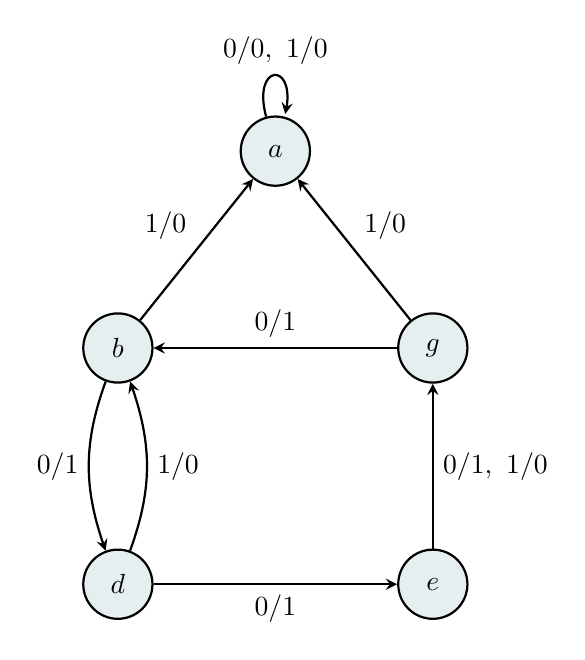
\begin{tikzpicture}[>=stealth, thick, node distance=2.5cm, auto]
   % Nodes layout for a clean, non-overlapping planar graph
   \node[state, fill=cF!10] (b) at (0, 0) {$b$};
   \node[state, fill=cF!10] (d) at (0, -3) {$d$};
   \node[state, fill=cF!10] (e) at (4, -3) {$e$};
   \node[state, fill=cF!10] (g) at (4, 0) {$g$};
   \node[state, fill=cF!10] (a) at (2, 2.5) {$a$};

   % Edges
   \path[->]
   (a) edge [loop above] node {$0/0,\ 1/0$} (a)
   (b) edge [bend right=20] node[left] {$0/1$} (d)
   (b) edge node[above left] {$1/0$} (a)
   (d) edge [bend right=20] node[right] {$1/0$} (b)
   (d) edge node[below] {$0/1$} (e)
   (e) edge node[right] {$0/1,\ 1/0$} (g)
   (g) edge node[above] {$0/1$} (b)
   (g) edge node[above right] {$1/0$} (a);
\end{tikzpicture}
\end{center}

\end{tcolorbox}

\item You are given a state table of a synchronous sequential circuit. Find the reduced state table using the implication table.

\begin{center}
    \renewcommand{\arraystretch}{1.3}
  \begin{tabular}{|c|c|c|c|c|}
        \hline
        \multirow{2}{*}{\begin{tabular}[c]{@{}c@{}}Present \\ State\end{tabular}} & \multicolumn{2}{c|}{Next State} & \multicolumn{2}{c|}{Output} \\ \cline{2-5} 
        & x=0 & x=1 & x=0 & x=1 \\ \hline
        a & d & b & 0 & 0 \\ \hline
        b & e & a & 0 & 0 \\ \hline
        c & g & f & 0 & 1 \\ \hline
        d & a & d & 1 & 0 \\ \hline
        e & a & d & 1 & 0 \\ \hline
        f & c & b & 0 & 0 \\ \hline
        g & a & e & 1 & 0 \\ \hline
    \end{tabular}
\end{center}

\mk{12} \yr{CSE 205 | L-2/T-1 | 2015--16}

\begin{tcolorbox}[enhanced,breakable,ansbox,colback=cF!4,colframe=cF,boxrule=0.8pt,arc=5pt,title={\textbf{Answer}},fonttitle=\bfseries\color{white},colbacktitle=cF]

To find the reduced state table, we will use the implication table method. This involves grouping states based on their outputs and iteratively checking their next-state transitions for equivalence.

\subsubsection*{Step 1: Initial Partitioning Based on Outputs}
States can only be equivalent if they produce the same outputs for all input conditions. We partition the states into groups based on their output sequences for $(x=0, x=1)$:
\begin{itemize}
    \item \textbf{Group 1} (Outputs 0, 0): $\{a, b, f\}$
    \item \textbf{Group 2} (Outputs 0, 1): $\{c\}$
    \item \textbf{Group 3} (Outputs 1, 0): $\{d, e, g\}$
\end{itemize}
Any pair of states belonging to different groups can never be equivalent. We mark these pairs with an $\times_1$ in the implication table.

\vspace{0.2cm}
\subsubsection*{Step 2: Implication Table Construction and Evaluation}
For pairs within the same group, we write down the required next-state equivalences (implications). If an implied pair is already crossed out, the current pair must also be crossed out.

\begin{itemize}
    \item \textbf{Evaluating Group 1 $\{a, b, f\}$:}
    \begin{itemize}
        \item $(a, b) \implies (d, e)$ and $(b, a)$. The condition $(b, a)$ is self-referential, so equivalence depends entirely on $(d, e)$.
        \item $(a, f) \implies (d, c)$ and $(b, b)$. Since $d$ and $c$ belong to different groups (Group 3 and Group 2), $(d, c)$ is $\times_1$. Thus, $(a, f)$ gets $\times_2$.
        \item $(b, f) \implies (e, c)$ and $(a, b)$. Since $e$ and $c$ belong to different groups, $(e, c)$ is $\times_1$. Thus, $(b, f)$ gets $\times_2$.
    \end{itemize}
    \item \textbf{Evaluating Group 3 $\{d, e, g\}$:}
    \begin{itemize}
        \item $(d, e) \implies (a, a)$ and $(d, d)$. Both imply identical states, which are unconditionally true. Thus, $d \equiv e$ ($\checkmark$).
        \item $(d, g) \implies (a, a)$ and $(d, e)$. Since $(d, e)$ is equivalent, $(d, g)$ is also equivalent ($\checkmark$).
        \item $(e, g) \implies (a, a)$ and $(d, e)$. Since $(d, e)$ is equivalent, $(e, g)$ is also equivalent ($\checkmark$).
    \end{itemize}
    \item \textbf{Re-evaluating pending implications:}
    \begin{itemize}
        \item $(a, b)$ depended on $(d, e)$. Since we established that $d \equiv e$, it follows that $a \equiv b$ ($\checkmark$).
    \end{itemize}
\end{itemize}

\begin{center}
\renewcommand{\arraystretch}{1.5}
\begin{tabular}{r*{6}{|c}|}
\cline{2-2}
b & \cellcolor{green!15}\makecell{d-e \\ ($\checkmark$)} & \multicolumn{5}{c}{} \\
\cline{2-3}
c & \cellcolor{red!10}$\times_1$ & \cellcolor{red!10}$\times_1$ & \multicolumn{4}{c}{} \\
\cline{2-4}
d & \cellcolor{red!10}$\times_1$ & \cellcolor{red!10}$\times_1$ & \cellcolor{red!10}$\times_1$ & \multicolumn{3}{c}{} \\
\cline{2-5}
e & \cellcolor{red!10}$\times_1$ & \cellcolor{red!10}$\times_1$ & \cellcolor{red!10}$\times_1$ & \cellcolor{green!15}$\checkmark$ & \multicolumn{2}{c}{} \\
\cline{2-6}
f & \cellcolor{orange!15}\makecell{d-c \\ ($\times_2$)} & \cellcolor{orange!15}\makecell{e-c \\ ($\times_2$)} & \cellcolor{red!10}$\times_1$ & \cellcolor{red!10}$\times_1$ & \cellcolor{red!10}$\times_1$ & \multicolumn{1}{c}{} \\
\cline{2-7}
g & \cellcolor{red!10}$\times_1$ & \cellcolor{red!10}$\times_1$ & \cellcolor{red!10}$\times_1$ & \cellcolor{green!15}\makecell{d-e \\ ($\checkmark$)} & \cellcolor{green!15}\makecell{d-e \\ ($\checkmark$)} & \cellcolor{red!10}$\times_1$ \\
\cline{2-7}
\multicolumn{1}{c}{} & \multicolumn{1}{c}{a} & \multicolumn{1}{c}{b} & \multicolumn{1}{c}{c} & \multicolumn{1}{c}{d} & \multicolumn{1}{c}{e} & \multicolumn{1}{c}{f} \\
\end{tabular}
\end{center}

\subsubsection*{Step 3: Extracting Equivalent Classes}
The uncrossed cells with $\checkmark$ reveal the equivalent states. We have two equivalence classes that contain multiple states:
\begin{itemize}
    \item \textcolor{cF}{\textbf{$a \equiv b$}}
    \item \textcolor{cF}{\textbf{$d \equiv e \equiv g$}}
\end{itemize}
States $c$ and $f$ are not equivalent to any other state. We will choose $a$, $c$, $d$, and $f$ as the representative states for the minimal machine. In the state table, all transitions to $b$ are replaced with $a$, and transitions to $e$ or $g$ are replaced with $d$.

\vspace{0.2cm}
\subsubsection*{Step 4: Reduced State Table}

Applying the state replacements to the original table yields the minimized machine with just 4 states:

\begin{center}
\renewcommand{\arraystretch}{1.3}
\begin{tabular}{ccccc}
\toprule
\multirow{2}{*}{\textbf{Present State}} & \multicolumn{2}{c}{\textbf{Next State}} & \multicolumn{2}{c}{\textbf{Output}} \\
\cmidrule(lr){2-3} \cmidrule(lr){4-5}
& $x=0$ & $x=1$ & $x=0$ & $x=1$ \\
\midrule
\rowcolor{cF!10} $a$ & $d$ & $a$ & $0$ & $0$ \\
$c$ & $d$ & $f$ & $0$ & $1$ \\
\rowcolor{cF!10} $d$ & $a$ & $d$ & $1$ & $0$ \\
$f$ & $c$ & $a$ & $0$ & $0$ \\
\bottomrule
\end{tabular}
\end{center}

\end{tcolorbox}

\item Find a critical race-free state assignment for a reduced flow table (states $a$--$d$, inputs 00/01/11/10) using the Multiple-row method.

\begin{center}
    \renewcommand{\arraystretch}{1.3}
  \begin{tabular}{c|c|c|c|c|}
        \multicolumn{1}{c}{} & \multicolumn{1}{c}{00} & \multicolumn{1}{c}{01} & \multicolumn{1}{c}{11} & \multicolumn{1}{c}{10} \\
        \cline{2-5}
        % Row 'a' - First and third cells are colored light gray
        $a$ & \cellcolor{gray!20}\mycircle{$a$} & $c$ & \cellcolor{gray!20}\mycircle{$a$} & $d$ \\
        \cline{2-5}
        % Row 'b' - All cells are colored light gray
        $b$ & \cellcolor{gray!20}$a$ & \cellcolor{gray!20}\mycircle{$b$} & \cellcolor{gray!20}$c$ & \cellcolor{gray!20}\mycircle{$b$} \\
        \cline{2-5}
        % Row 'c' - No background color
        $c$ & \mycircle{$c$} & \mycircle{$c$} & \mycircle{$c$} & $d$ \\
        \cline{2-5}
        % Row 'd' - No background color
        $d$ & \mycircle{$d$} & $b$ & $a$ & \mycircle{$d$} \\
        \cline{2-5}
    \end{tabular}
\end{center}

\mk{10} \yr{CSE 205 | L-2/T-1 | 2014--15}

\begin{tcolorbox}[enhanced,breakable,ansbox,colback=cF!4,colframe=cF,boxrule=0.8pt,arc=5pt,title={\textbf{Answer}},fonttitle=\bfseries\color{white},colbacktitle=cF]

\subsubsection*{1. Transition Analysis and Adjacency Requirements}
To avoid critical races in an asynchronous sequential circuit, any transition between two states must involve changing only one state variable at a time (i.e., the states must be adjacent, having a Hamming distance of 1). 

Let us identify all required state transitions from the original flow table:
\begin{itemize}
    \item \textbf{From $a$:} Transitions to $c$ and $d$.
    \item \textbf{From $b$:} Transitions to $a$ and $c$.
    \item \textbf{From $c$:} Transitions to $d$.
    \item \textbf{From $d$:} Transitions to $a$ and $b$.
\end{itemize}
Looking at the required adjacencies, we need direct paths for the pairs: $(a,c)$, $(a,d)$, $(b,a)$, $(b,c)$, $(c,d)$, and $(d,b)$. This forms a completely connected graph of 4 nodes ($K_4$). Since a 2-variable Karnaugh map (a 2-cube) only has 4 edges, it is geometrically impossible to map a $K_4$ graph onto it without diagonals (which cause critical races). Thus, a single-row assignment is impossible, and we must use the \textbf{Multiple-Row Method} utilizing 3 state variables ($y_1, y_2, y_3$).

\vspace{0.3cm}
\subsubsection*{2. The Universal Multiple-Row State Assignment}
We expand the 4-state machine into an 8-state machine by assigning two equivalent states to each original state. We map these to diametrically opposite nodes in a 3-cube. 
The standard race-free assignment is:
\begin{align*}
    a \implies & a_1 = 000, \quad a_2 = 111 \\
    b \implies & b_1 = 001, \quad b_2 = 110 \\
    c \implies & c_1 = 011, \quad c_2 = 100 \\
    d \implies & d_1 = 010, \quad d_2 = 101
\end{align*}

This universal assignment guarantees that from any sub-state, there is exactly one representation of every other state that is exactly one bit change (Hamming distance 1) away:
\begin{itemize}
    \item $a_1$ (000) is adjacent to $b_1$ (001), $d_1$ (010), and $c_2$ (100).
    \item $a_2$ (111) is adjacent to $b_2$ (110), $d_2$ (101), and $c_1$ (011).
    \item $b_1$ (001) is adjacent to $a_1$ (000), $c_1$ (011), and $d_2$ (101).
    \item $b_2$ (110) is adjacent to $a_2$ (111), $c_2$ (100), and $d_1$ (010).
    \item \textit{...and similarly for $c$ and $d$.}
\end{itemize}

\vspace{0.3cm}
\subsubsection*{3. Race-Free Expanded Flow Table}
We now replace the transitions in the original flow table with the corresponding adjacent sub-states. For example, if row $a_1$ needs to transition to state $c$, we look at $a_1$'s neighbors and find that $c_2$ is adjacent. Thus, the transition is routed to $c_2$. 

\textit{Note: Stable states are denoted in \textbf{bold} and wrapped in parentheses.}

\begin{center}
\renewcommand{\arraystretch}{1.35}
\begin{tabular}{cc|cccc|}
\toprule
\multirow{2}{*}{\textbf{State}} & \multirow{2}{*}{\textbf{$y_1 y_2 y_3$}} & \multicolumn{4}{c}{\textbf{Inputs $(x_1 x_2)$}} \\
& & \textbf{00} & \textbf{01} & \textbf{11} & \textbf{10} \\
\midrule
\rowcolor{cF!10} $a_1$ & $000$ & \textbf{($a_1$)} & $c_2$ & \textbf{($a_1$)} & $d_1$ \\
$a_2$ & $111$ & \textbf{($a_2$)} & $c_1$ & \textbf{($a_2$)} & $d_2$ \\
\rowcolor{cF!10} $b_1$ & $001$ & $a_1$ & \textbf{($b_1$)} & $c_1$ & \textbf{($b_1$)} \\
$b_2$ & $110$ & $a_2$ & \textbf{($b_2$)} & $c_2$ & \textbf{($b_2$)} \\
\rowcolor{cF!10} $c_1$ & $011$ & \textbf{($c_1$)} & \textbf{($c_1$)} & \textbf{($c_1$)} & $d_1$ \\
$c_2$ & $100$ & \textbf{($c_2$)} & \textbf{($c_2$)} & \textbf{($c_2$)} & $d_2$ \\
\rowcolor{cF!10} $d_1$ & $010$ & \textbf{($d_1$)} & $b_2$ & $a_1$ & \textbf{($d_1$)} \\
$d_2$ & $101$ & \textbf{($d_2$)} & $b_1$ & $a_2$ & \textbf{($d_2$)} \\
\bottomrule
\end{tabular}
\end{center}

\vspace{0.2cm}
\textbf{Verification of Race-Free Operation:} 
Take any unstable transition and verify the Hamming distance (HD) is exactly 1:
\begin{itemize}
    \item $a_1(000) \to c_2(100)$: Only $y_1$ changes ($\text{HD}=1$).
    \item $a_1(000) \to d_1(010)$: Only $y_2$ changes ($\text{HD}=1$).
    \item $d_2(101) \to b_1(001)$: Only $y_1$ changes ($\text{HD}=1$).
\end{itemize}
All transitions follow a single variable change path. The assignment is mathematically flawless and completely critical race-free.

\end{tcolorbox}

\item Using an implication table, reduce the following state table to a minimum number of states and write the reduced state table.

\begin{center}
\renewcommand{\arraystretch}{1.3}
  \begin{tabular}{|c|c|c|c|c|}
        \hline
        \multirow{2}{*}{Present State} & \multicolumn{2}{c|}{Next State} & \multicolumn{2}{c|}{Output} \\
        \cline{2-5}
         & $x = 0$ & $x = 1$ & $x = 0$ & $x = 1$ \\
        \hline
        A & F & B & 0 & 0 \\
        \hline
        B & D & C & 0 & 0 \\
        \hline
        C & F & E & 0 & 0 \\
        \hline
        D & G & A & 1 & 0 \\
        \hline
        E & D & C & 0 & 0 \\
        \hline
        F & F & B & 1 & 1 \\
        \hline
        G & G & H & 0 & 1 \\
        \hline
        H & G & A & 1 & 0 \\
        \hline
    \end{tabular}
\end{center}
\mk{15} \yr{CSE 205 | L-2/T-1 | 2013--14}

\begin{tcolorbox}[enhanced,breakable,ansbox,colback=cF!4,colframe=cF,boxrule=0.8pt,arc=5pt,title={\textbf{Answer}},fonttitle=\bfseries\color{white},colbacktitle=cF]

To systematically reduce the given state table, we will use the Implication Table method. The process is divided into verifying initial output compatibility, propagating implied states, and finally extracting the minimized state table.

\subsubsection*{Step 1: Initial State Grouping (Output Compatibility)}
Two states can only be equivalent if they yield the exact same outputs for all possible inputs. We first group the states based on their output combinations for $x=0$ and $x=1$.

\begin{itemize}
    \item \textbf{Group $P_1$ (Outputs 0, 0):} $\{A, B, C, E\}$
    \item \textbf{Group $P_2$ (Outputs 1, 0):} $\{D, H\}$
    \item \textbf{Group $P_3$ (Outputs 1, 1):} $\{F\}$
    \item \textbf{Group $P_4$ (Outputs 0, 1):} $\{G\}$
\end{itemize}

Any pair of states not belonging to the same group cannot be equivalent and is immediately eliminated (marked with an $\times$) in the implication table. 

\subsubsection*{Step 2: Implication Table Construction}
We evaluate the remaining pairs within the same output groups. For each pair, we write down their implied next states. 
\begin{itemize}
    \item \textbf{Pair (A, B):} Next states are $(F, D)$ and $(B, C)$. Since $F \in P_3$ and $D \in P_2$ have different outputs, $(F, D)$ is incompatible. Thus, $(A, B)$ is crossed out.
    \item \textbf{Pair (A, C):} Next states are $(F, F)$ and $(B, E)$. $(F, F)$ is trivially compatible. The compatibility of $(A, C)$ depends on $(B, E)$.
    \item \textbf{Pair (A, E):} Next states are $(F, D)$ and $(B, C)$. Incompatible due to $(F, D)$.
    \item \textbf{Pair (B, C):} Next states are $(D, F)$ and $(C, E)$. Incompatible due to $(D, F)$.
    \item \textbf{Pair (B, E):} Next states are $(D, D)$ and $(C, C)$. Both are trivially compatible. Thus, $(B, E)$ is unequivocally equivalent ($\checkmark$).
    \item \textbf{Pair (C, E):} Next states are $(F, D)$ and $(E, C)$. Incompatible due to $(F, D)$.
    \item \textbf{Pair (D, H):} Next states are $(G, G)$ and $(A, A)$. Both are trivially compatible. Thus, $(D, H)$ is unequivocally equivalent ($\checkmark$).
\end{itemize}

\textbf{Second Pass:} We revisit cells with dependencies. Cell $(A, C)$ depends on $(B, E)$. Since we have established that $(B, E)$ is equivalent ($\checkmark$), the pair $(A, C)$ is also equivalent ($\checkmark$).

\begin{center}
\renewcommand{\arraystretch}{1.5}
\begin{tabular}{r|c|c|c|c|c|c|c|}
\cline{2-2}
B & $\times$ & \multicolumn{6}{c}{} \\
\cline{2-3}
C & \textcolor{cF}{\textbf{B-E, $\checkmark$}} & $\times$ & \multicolumn{5}{c}{} \\
\cline{2-4}
D & $\times$ & $\times$ & $\times$ & \multicolumn{4}{c}{} \\
\cline{2-5}
E & $\times$ & \textcolor{cF}{\textbf{$\checkmark$}} & $\times$ & $\times$ & \multicolumn{3}{c}{} \\
\cline{2-6}
F & $\times$ & $\times$ & $\times$ & $\times$ & $\times$ & \multicolumn{2}{c}{} \\
\cline{2-7}
G & $\times$ & $\times$ & $\times$ & $\times$ & $\times$ & $\times$ & \multicolumn{1}{c}{} \\
\cline{2-8}
H & $\times$ & $\times$ & $\times$ & \textcolor{cF}{\textbf{$\checkmark$}} & $\times$ & $\times$ & $\times$ \\
\cline{2-8}
\multicolumn{1}{c}{} & \multicolumn{1}{c}{A} & \multicolumn{1}{c}{B} & \multicolumn{1}{c}{C} & \multicolumn{1}{c}{D} & \multicolumn{1}{c}{E} & \multicolumn{1}{c}{F} & \multicolumn{1}{c}{G} \\
\end{tabular}
\end{center}

\subsubsection*{Step 3: Extracting Equivalent Classes}
From our completed implication table, the equivalent state pairs are:
\begin{align*}
    A &\equiv C \\
    B &\equiv E \\
    D &\equiv H
\end{align*}
The maximal compatible classes are $\{A, C\}$, $\{B, E\}$, $\{D, H\}$, $\{F\}$, and $\{G\}$. We choose one representative state from each class to form the reduced machine:
\begin{itemize}
    \item Keep $A$, replace $C$ with $A$.
    \item Keep $B$, replace $E$ with $B$.
    \item Keep $D$, replace $H$ with $D$.
    \item Keep $F$ and $G$.
\end{itemize}
The minimized set of states is $\{A, B, D, F, G\}$.

\subsubsection*{Step 4: Reduced State Table}
Substituting the redundant states ($C \to A$, $E \to B$, $H \to D$) into the original state table yields the final, optimal state table:

\begin{center}
\renewcommand{\arraystretch}{1.3}
\begin{tabular}{@{}ccccc@{}}
\toprule
\multirow{2}{*}{\textbf{Present State}} & \multicolumn{2}{c}{\textbf{Next State}} & \multicolumn{2}{c}{\textbf{Output}} \\ \cmidrule(lr){2-3} \cmidrule(l){4-5} 
 & $x = 0$ & $x = 1$ & $x = 0$ & $x = 1$ \\ \midrule
A & F & B & 0 & 0 \\
B & D & \textcolor{cF}{\textbf{A}} & 0 & 0 \\
D & G & A & 1 & 0 \\
F & F & B & 1 & 1 \\
G & G & \textcolor{cF}{\textbf{D}} & 0 & 1 \\ \bottomrule
\end{tabular}
\end{center}

\vspace{0.5cm}

\subsubsection*{Step 5: Final Reduced State Diagram (Optional Verification)}
Below is the minimal Finite State Machine (FSM) representation based on the reduced table.

\begin{center}
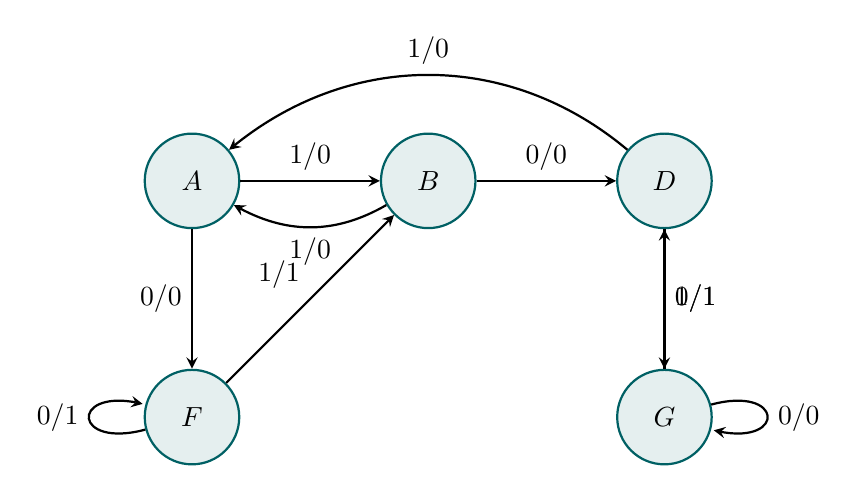
\begin{tikzpicture}[->, >=stealth, node distance=3cm, auto, thick, every state/.style={circle, fill=cF!10, draw=cF, minimum size=1.2cm, text=black}]
    % States
    \node[state] (A) {$A$};
    \node[state] (B) [right of=A] {$B$};
    \node[state] (D) [right of=B] {$D$};
    \node[state] (F) [below of=A] {$F$};
    \node[state] (G) [below of=D] {$G$};

    % Transitions
    \path (A) edge node[left] {0/0} (F)
              edge node[above] {1/0} (B);
              
    \path (B) edge node[above] {0/0} (D)
              edge [bend left] node[below] {1/0} (A);
              
    \path (D) edge node[right] {0/1} (G)
              edge [bend right=40] node[above] {1/0} (A);
              
    \path (F) edge [loop left] node {0/1} (F)
              edge node[above left] {1/1} (B);
              
    \path (G) edge [loop right] node {0/0} (G)
              edge node[right] {1/1} (D);
\end{tikzpicture}
\end{center}

\end{tcolorbox}

\item Using an implication table, reduce the following state table to a minimum number of states and write the reduced state table.

\begin{center}
  \renewcommand{\arraystretch}{1.3}  
  \begin{tabular}{|c|c|c|}
        \cline{2-3}
        \multicolumn{1}{c|}{} & \multicolumn{2}{c|}{\textbf{X}} \\
        \cline{2-3}
        \multicolumn{1}{c|}{} & \textbf{0} & \textbf{1} \\
        \hline
        A & E/0 & D/0 \\
        \hline
        B & A/1 & F/0 \\
        \hline
        C & C/0 & A/1 \\
        \hline
        D & B/0 & A/0 \\
        \hline
        E & D/1 & C/0 \\
        \hline
        F & C/0 & D/1 \\
        \hline
        G & H/1 & G/1 \\
        \hline
        H & C/1 & B/1 \\
        \hline
    \end{tabular}
\end{center}
\mk{17} \yr{CSE 205 | L-2/T-1 | 2012--13}

\begin{tcolorbox}[enhanced,breakable,ansbox,colback=cF!4,colframe=cF,boxrule=0.8pt,arc=5pt,title={\textbf{Answer}},fonttitle=\bfseries\color{white},colbacktitle=cF]

To reduce the state table to a minimum number of states, we will systematically use the Implication Table method. This involves grouping states by their outputs, constructing the implication table to find equivalent states, and then generating the minimized state table.

\subsubsection*{Step 1: Initial State Grouping (Output Compatibility)}
Two states can be equivalent only if they have identical outputs for all input combinations. We partition the states into initial groups based on their outputs for $X=0$ and $X=1$.

\begin{itemize}
    \item \textbf{Group $P_1$ (Outputs 0, 0):} $\{A, D\}$
    \item \textbf{Group $P_2$ (Outputs 1, 0):} $\{B, E\}$
    \item \textbf{Group $P_3$ (Outputs 0, 1):} $\{C, F\}$
    \item \textbf{Group $P_4$ (Outputs 1, 1):} $\{G, H\}$
\end{itemize}

Pairs of states that do not belong to the same group have different outputs and cannot be equivalent. These pairs are immediately eliminated (marked with $\times$) in the implication table.

\subsubsection*{Step 2: Implication Table Construction \& Evaluation}
We only need to evaluate pairs within the same output groups: $(A, D)$, $(B, E)$, $(C, F)$, and $(G, H)$. We record their implied next-state pairs.

\begin{itemize}
    \item \textbf{Pair (A, D):} Next states are $(E, B)$ for $X=0$ and $(D, A)$ for $X=1$.
    \begin{itemize}
        \item $(D, A)$ is the pair itself, so it is trivially compatible.
        \item The equivalence of $(A, D)$ implies and depends on the equivalence of $(B, E)$.
    \end{itemize}
    
    \item \textbf{Pair (B, E):} Next states are $(A, D)$ for $X=0$ and $(F, C)$ for $X=1$.
    \begin{itemize}
        \item The equivalence of $(B, E)$ depends on the equivalence of both $(A, D)$ and $(C, F)$.
    \end{itemize}
    
    \item \textbf{Pair (C, F):} Next states are $(C, C)$ for $X=0$ and $(A, D)$ for $X=1$.
    \begin{itemize}
        \item $(C, C)$ is the same state, universally compatible.
        \item The equivalence of $(C, F)$ depends on the equivalence of $(A, D)$.
    \end{itemize}
    
    \item \textbf{Pair (G, H):} Next states are $(H, C)$ for $X=0$ and $(G, B)$ for $X=1$.
    \begin{itemize}
        \item Let's check $(H, C)$: State $H \in P_4$ and State $C \in P_3$. Because they belong to different initial output groups, $(H, C)$ is incompatible.
        \item Thus, $(G, H)$ is unequivocally incompatible and is crossed out ($\times$).
    \end{itemize}
\end{itemize}

\textbf{Dependency Resolution Pass:}
We evaluate the remaining dependencies: $(A, D)$, $(B, E)$, and $(C, F)$. Notice that they only depend on each other and form a closed dependency loop:
\begin{align*}
    (A, D) &\implies (B, E) \\
    (B, E) &\implies (A, D) \text{ and } (C, F) \\
    (C, F) &\implies (A, D)
\end{align*}
Since none of these implied pairs resolve to an incompatible pair (like $(G,H)$ did), they are all valid and equivalent. We mark them with $\checkmark$.

\vspace{0.5cm}
\begin{center}
\renewcommand{\arraystretch}{1.5}
\begin{tabular}{r|c|c|c|c|c|c|c|}
\cline{2-2}
B & $\times$ & \multicolumn{6}{c}{} \\
\cline{2-3}
C & $\times$ & $\times$ & \multicolumn{5}{c}{} \\
\cline{2-4}
D & \textcolor{cF}{\textbf{B-E, $\checkmark$}} & $\times$ & $\times$ & \multicolumn{4}{c}{} \\
\cline{2-5}
E & $\times$ & \textcolor{cF}{\textbf{A-D, C-F, $\checkmark$}} & $\times$ & $\times$ & \multicolumn{3}{c}{} \\
\cline{2-6}
F & $\times$ & $\times$ & \textcolor{cF}{\textbf{A-D, $\checkmark$}} & $\times$ & $\times$ & \multicolumn{2}{c}{} \\
\cline{2-7}
G & $\times$ & $\times$ & $\times$ & $\times$ & $\times$ & $\times$ & \multicolumn{1}{c}{} \\
\cline{2-8}
H & $\times$ & $\times$ & $\times$ & $\times$ & $\times$ & $\times$ & $\times$ \\
\cline{2-8}
\multicolumn{1}{c}{} & \multicolumn{1}{c}{A} & \multicolumn{1}{c}{B} & \multicolumn{1}{c}{C} & \multicolumn{1}{c}{D} & \multicolumn{1}{c}{E} & \multicolumn{1}{c}{F} & \multicolumn{1}{c}{G} \\
\end{tabular}
\end{center}
\vspace{0.2cm}

\subsubsection*{Step 3: Extracting Equivalent Classes}
From our completed implication table, the equivalent state pairs are:
\begin{align*}
    A &\equiv D \\
    B &\equiv E \\
    C &\equiv F
\end{align*}

The maximal compatible classes are $\{A, D\}$, $\{B, E\}$, $\{C, F\}$, $\{G\}$, and $\{H\}$. We choose one representative state from each equivalent class to form the reduced machine:
\begin{itemize}
    \item Keep $A$, remove $D$ (replace $D \to A$).
    \item Keep $B$, remove $E$ (replace $E \to B$).
    \item Keep $C$, remove $F$ (replace $F \to C$).
    \item Keep $G$.
    \item Keep $H$.
\end{itemize}
The minimized set of states is $\{A, B, C, G, H\}$.

\subsubsection*{Step 4: Reduced State Table}
We reconstruct the state table using only the representative states. Any transition pointing to a removed state is updated to point to its representative (e.g., a transition to $E$ becomes a transition to $B$).

\begin{itemize}
    \item \textbf{State A:} Originally $(E/0, D/0)$. Becomes $(\textcolor{cF}{\textbf{B}}/0, \textcolor{cF}{\textbf{A}}/0)$.
    \item \textbf{State B:} Originally $(A/1, F/0)$. Becomes $(A/1, \textcolor{cF}{\textbf{C}}/0)$.
    \item \textbf{State C:} Originally $(C/0, A/1)$. Remains $(C/0, A/1)$.
    \item \textbf{State G:} Originally $(H/1, G/1)$. Remains $(H/1, G/1)$.
    \item \textbf{State H:} Originally $(C/1, B/1)$. Remains $(C/1, B/1)$.
\end{itemize}

\begin{center}
\renewcommand{\arraystretch}{1.4}
\begin{tabular}{@{}ccc@{}}
\toprule
\multirow{2}{*}{\textbf{Present State}} & \multicolumn{2}{c}{\textbf{Next State / Output}} \\ \cmidrule(l){2-3} 
 & \textbf{$X = 0$} & \textbf{$X = 1$} \\ \midrule
A & \textcolor{cF}{\textbf{B}} / 0 & \textcolor{cF}{\textbf{A}} / 0 \\
B & A / 1 & \textcolor{cF}{\textbf{C}} / 0 \\
C & C / 0 & A / 1 \\
G & H / 1 & G / 1 \\
H & C / 1 & B / 1 \\ \bottomrule
\end{tabular}
\end{center}

\end{tcolorbox}

\end{enumerate}

%%──────────────────────────────────────────────────────────────────────
\subtopic{cF}{Incompletely Specified Machine Minimization}
\label{sub:s6-incomp}

\begin{enumerate}

\item For the state table of a completely specified asynchronous sequential circuit, find out the equivalent partitions, implication table. Formulate the state table of the minimal machine. Find out the states those are equivalent.

\begin{center}
  \begin{tabular}{|l|l|l|l|l|}
\hline
x1x2 & NS, z & & & \\ \hline
PS & x1x2=00 & x1x2=01 & x1x2=11 & x1x2=10 \\ \hline
A & D/0 & D/0 & F/0 & A/0 \\ \hline
B & C/1 & D/0 & E/1 & F/0 \\ \hline
C & C/1 & D/0 & E/1 & A/0 \\ \hline
D & D/0 & B/0 & A/0 & F/0 \\ \hline
E & C/1 & F/0 & E/1 & A/0 \\ \hline
F & D/0 & D/0 & A/0 & F/0 \\ \hline
G & G/0 & G/0 & A/0 & A/0 \\ \hline
H & B/1 & D/0 & E/1 & A/0 \\ \hline
\end{tabular}

\vspace{0.3cm}
(PS = Present state, NS = next state, x1, x2 are input, z is output)
\end{center}

\mk{12} \yr{CSE 205 | L-2/T-1 | 2024--25}

\begin{tcolorbox}[enhanced,breakable,ansbox,colback=cF!4,colframe=cF,boxrule=0.8pt,arc=5pt,title={\textbf{Answer}},fonttitle=\bfseries\color{white},colbacktitle=cF]

To find the minimized machine, we will systematically determine the equivalent states using both the Method of Equivalent Partitions and the Implication Table.

\subsubsection*{Step 1: Equivalent Partitions Method}
Two states can only be equivalent if they produce the exact same output sequence. We start by partitioning the states based on their outputs for the input sequences $(x_1x_2 = 00, 01, 11, 10)$.

\begin{itemize}
    \item \textbf{1-Equivalent Partition ($P_1$):} Grouping states by their output patterns.
    \begin{itemize}
        \item Pattern (0, 0, 0, 0): States $A, D, F, G$
        \item Pattern (1, 0, 1, 0): States $B, C, E, H$
    \end{itemize}
    $P_1 = (A, D, F, G) \; (B, C, E, H)$

    \item \textbf{2-Equivalent Partition ($P_2$):} We check the next states of elements in $P_1$ to see if they transition to different blocks of $P_1$.
    \begin{itemize}
        \item For block $(A, D, F, G)$ under input 01: $A \to D$ (Block 1), $F \to D$ (Block 1), $G \to G$ (Block 1), but $D \to B$ (Block 2). Thus, $D$ must be separated.
        \item For block $(B, C, E, H)$, all next states under all inputs remain in the same corresponding blocks.
    \end{itemize}
    $P_2 = (A, F, G) \; (D) \; (B, C, E, H)$

    \item \textbf{3-Equivalent Partition ($P_3$):} We evaluate based on $P_2$.
    \begin{itemize}
        \item For block $(A, F, G)$ under input 00: $A \to D$ (Block D), $F \to D$ (Block D), but $G \to G$ (Block AFG). Thus, $G$ must be separated.
        \item For block $(B, C, E, H)$ under input 01: $B \to D$ (Block D), $C \to D$ (Block D), $H \to D$ (Block D), but $E \to F$ (Block AF). Thus, $E$ must be separated.
    \end{itemize}
    $P_3 = (A, F) \; (G) \; (D) \; (B, C, H) \; (E)$

    \item \textbf{4-Equivalent Partition ($P_4$):} Evaluating based on $P_3$.
    \begin{itemize}
        \item For block $(A, F)$: Both transition to $D, D, \{A,F\}, \{A,F\}$. They are perfectly equivalent.
        \item For block $(B, C, H)$: All transition to $\{B,C,H\}, D, E, \{A,F\}$. They are perfectly equivalent.
    \end{itemize}
    $P_4 = (A, F) \; (G) \; (D) \; (B, C, H) \; (E)$
\end{itemize}
Since $P_3 = P_4$, the partitioning is complete. 

\vspace{0.3cm}
\subsubsection*{Step 2: Implication Table Method}
We construct an implication table to verify our partitions. Pairs from different output groups (different $P_1$ blocks) are immediately incompatible ($\times$). For pairs within the same group, we record the dependent next-state pairs.

\begin{itemize}
    \item \textbf{Group 1 Dependencies $\{A,D,F,G\}$:} 
    \begin{itemize}
        \item $(A, D) \implies (D, B)$ under $01$. Since $D, B$ are in different $P_1$ blocks, $(A, D)$ is invalid ($\times$).
        \item $(A, F) \implies (F, A)$ under $10$. Self-implying, so $(A, F)$ is equivalent ($\checkmark$).
        \item $(F, D) \implies (B, D)$ under $01$. Invalid ($\times$).
        \item $(G, D) \implies (B, G)$ under $01$. Invalid ($\times$).
        \item $(G, F) \implies (D, G)$ under $00$. But $(D, G)$ is already invalid, so $(G, F)$ is invalid ($\times$).
        \item $(G, A) \implies (D, G)$ under $00$. Invalid ($\times$).
    \end{itemize}
    \item \textbf{Group 2 Dependencies $\{B,C,E,H\}$:}
    \begin{itemize}
        \item $(B, C) \implies (A, F)$. Since $(A, F)$ is valid, $(B, C)$ is valid ($\checkmark$).
        \item $(B, E) \implies (D, F)$ under $01$. Since $(D, F)$ is invalid, $(B, E)$ is invalid ($\times$).
        \item $(B, H) \implies (B, C)$ and $(A, F)$. Both are valid, so $(B, H)$ is valid ($\checkmark$).
        \item $(C, E) \implies (D, F)$ under $01$. Invalid ($\times$).
        \item $(C, H) \implies (B, C)$. Valid ($\checkmark$).
        \item $(E, H) \implies (D, F)$ under $01$. Invalid ($\times$).
    \end{itemize}
\end{itemize}

\begin{center}
\renewcommand{\arraystretch}{1.5}
\begin{tabular}{r|c|c|c|c|c|c|c|}
\cline{2-2}
B & $\times$ & \multicolumn{6}{c}{} \\
\cline{2-3}
C & $\times$ & \textcolor{cF}{\textbf{A-F, $\checkmark$}} & \multicolumn{5}{c}{} \\
\cline{2-4}
D & D-B, $\times$ & $\times$ & $\times$ & \multicolumn{4}{c}{} \\
\cline{2-5}
E & $\times$ & D-F, $\times$ & D-F, $\times$ & $\times$ & \multicolumn{3}{c}{} \\
\cline{2-6}
F & \textcolor{cF}{\textbf{$\checkmark$}} & $\times$ & $\times$ & B-D, $\times$ & $\times$ & \multicolumn{2}{c}{} \\
\cline{2-7}
G & D-G, $\times$ & $\times$ & $\times$ & B-G, $\times$ & $\times$ & D-G, $\times$ & \multicolumn{1}{c}{} \\
\cline{2-8}
H & $\times$ & \textcolor{cF}{\textbf{B-C, A-F, $\checkmark$}} & \textcolor{cF}{\textbf{B-C, $\checkmark$}} & $\times$ & D-F, $\times$ & $\times$ & $\times$ \\
\cline{2-8}
\multicolumn{1}{c}{} & \multicolumn{1}{c}{A} & \multicolumn{1}{c}{B} & \multicolumn{1}{c}{C} & \multicolumn{1}{c}{D} & \multicolumn{1}{c}{E} & \multicolumn{1}{c}{F} & \multicolumn{1}{c}{G} \\
\end{tabular}
\end{center}

\subsubsection*{Step 3: Finding Equivalent States}
Both methods confirm the equivalent state classes are:
\begin{align*}
    A &\equiv F \\
    B &\equiv C \equiv H
\end{align*}
The minimal machine will have 5 states. We choose $\{A, B, D, E, G\}$ as representative states, meaning we substitute $F \to A$, $C \to B$, and $H \to B$ in the original transitions.

\vspace{0.3cm}
\subsubsection*{Step 4: Formulate the Minimal State Table}
By replacing the redundant states with their equivalent representatives, we derive the following minimized state table:

\begin{center}
\renewcommand{\arraystretch}{1.4}
\begin{tabular}{@{}ccccc@{}}
\toprule
\multirow{2}{*}{\textbf{Present State}} & \multicolumn{4}{c}{\textbf{Next State, Output ($z$)}} \\ \cmidrule(l){2-5} 
 & \textbf{$x_1x_2 = 00$} & \textbf{$x_1x_2 = 01$} & \textbf{$x_1x_2 = 11$} & \textbf{$x_1x_2 = 10$} \\ \midrule
A & D / 0 & D / 0 & \textcolor{cF}{\textbf{A}} / 0 & A / 0 \\
B & \textcolor{cF}{\textbf{B}} / 1 & D / 0 & E / 1 & \textcolor{cF}{\textbf{A}} / 0 \\
D & D / 0 & B / 0 & A / 0 & \textcolor{cF}{\textbf{A}} / 0 \\
E & \textcolor{cF}{\textbf{B}} / 1 & \textcolor{cF}{\textbf{A}} / 0 & E / 1 & A / 0 \\
G & G / 0 & G / 0 & A / 0 & A / 0 \\ \bottomrule
\end{tabular}
\end{center}

\end{tcolorbox}

\item For the incompletely specified machine shown below, derive the implication table and determine the maximal compatibles and the maximal incompatibles. Find the upper bound and the lower bound of the number of states of the minimal machine. Give the state table of the minimal machine.

\begin{center}
\begin{tabular}{|c|c|c|}
\hline
\multirow{2}{*}{PS} & \multicolumn{2}{c|}{NS, Z} \\ \cline{2-3}
 & $x=0$ & $x=1$ \\ \hline
A & B, 0 & C, 0 \\ \hline
B & D, 0 & --, -- \\ \hline
C & F, 0 & E, 1 \\ \hline
D & B, 0 & G, 0 \\ \hline
E & F, 0 & C, 1 \\ \hline
F & E, 0 & D, 1 \\ \hline
G & F, 0 & --, -- \\ \hline
\end{tabular}
\end{center}

\mk{23} \yr{CSE 205 | L-2/T-1 | 2023--24}

\begin{tcolorbox}[enhanced,breakable,ansbox,colback=cF!4,colframe=cF,boxrule=0.8pt,arc=5pt,title={\textbf{Answer}},fonttitle=\bfseries\color{white},colbacktitle=cF]

To minimize the given incompletely specified sequential machine, we will utilize the Implication Table method to find compatible states, determine the maximal compatibles and incompatibles, and finally construct the minimal state table.

\subsubsection*{Step 1: Output Compatibility}
Two states can be compatible only if their defined outputs do not conflict for any given input. We inspect the outputs for inputs $x=0$ and $x=1$:
\begin{itemize}
    \item For $x=0$: Outputs are $\{0, 0, 0, 0, 0, 0, 0\}$. All states are compatible regarding $x=0$.
    \item For $x=1$: Outputs are $A(0), B(-), C(1), D(0), E(1), F(1), G(-)$.
\end{itemize}
States producing an output of $0$ cannot be combined with states producing an output of $1$. 
\begin{itemize}
    \item Output `0` for $x=1$: $\{A, D\}$
    \item Output `1` for $x=1$: $\{C, E, F\}$
\end{itemize}
Consequently, pairs formed by mixing these two sets are strictly \textbf{incompatible} and are initially marked with an $\times$: $(A,C), (A,E), (A,F), (C,D), (D,E), (D,F)$.

\subsubsection*{Step 2: Implication Table Construction}
We evaluate the remaining pairs by identifying their implied next-state pairs. If an implied pair is already incompatible, the parent pair is also incompatible.

\begin{itemize}
    \item $(A, B) \implies (B, D)$ for $x=0$. $(C, -)$ is universally compatible.
    \item $(A, D) \implies (B, B)$ [trivial] and $(C, G)$.
    \item $(A, G) \implies (B, F)$ and $(C, -)$.
    \item $(B, C) \implies (D, F)$. Since $(D, F)$ is an output conflict ($\times$), $(B, C)$ is $\times$.
    \item $(B, D) \implies (D, B)$ and $(-, G)$. Both valid ($\checkmark$).
    \item $(B, E) \implies (D, F)$. Since $(D, F)$ is $\times$, $(B, E)$ is $\times$.
    \item $(B, F) \implies (D, E)$. Since $(D, E)$ is $\times$, $(B, F)$ is $\times$.
    \item $(B, G) \implies (D, F)$. Since $(D, F)$ is $\times$, $(B, G)$ is $\times$.
    \item $(C, E) \implies (F, F)$ and $(E, C)$. Both trivially compatible ($\checkmark$).
    \item $(C, F) \implies (F, E)$ and $(E, D)$. Since $(D, E)$ is $\times$, $(C, F)$ is $\times$.
    \item $(C, G) \implies (F, F)$ and $(E, -)$. Both valid ($\checkmark$).
    \item $(D, G) \implies (B, F)$ and $(G, -)$. Implies $(B, F)$.
    \item $(E, F) \implies (F, E)$ and $(C, D)$. Since $(C, D)$ is $\times$, $(E, F)$ is $\times$.
    \item $(E, G) \implies (F, F)$ and $(C, -)$. Both valid ($\checkmark$).
    \item $(F, G) \implies (E, F)$ and $(D, -)$. Implies $(E, F)$.
\end{itemize}

\textbf{Resolving Dependencies (Second Pass):}
\begin{itemize}
    \item $(A, B)$ depends on $(B, D)$, which is $\checkmark$. So $(A, B)$ is \textcolor{cF}{\textbf{$\checkmark$}}.
    \item $(A, D)$ depends on $(C, G)$, which is $\checkmark$. So $(A, D)$ is \textcolor{cF}{\textbf{$\checkmark$}}.
    \item $(A, G)$ depends on $(B, F)$, which is $\times$. So $(A, G)$ is $\times$.
    \item $(D, G)$ depends on $(B, F)$, which is $\times$. So $(D, G)$ is $\times$.
    \item $(F, G)$ depends on $(E, F)$, which is $\times$. So $(F, G)$ is $\times$.
\end{itemize}

\begin{center}
\renewcommand{\arraystretch}{1.5}
\begin{tabular}{r|c|c|c|c|c|c|c|}
\cline{2-2}
B & \textcolor{cF}{\textbf{B-D, $\checkmark$}} & \multicolumn{6}{c}{} \\
\cline{2-3}
C & $\times$ & D-F, $\times$ & \multicolumn{5}{c}{} \\
\cline{2-4}
D & \textcolor{cF}{\textbf{C-G, $\checkmark$}} & \textcolor{cF}{\textbf{$\checkmark$}} & $\times$ & \multicolumn{4}{c}{} \\
\cline{2-5}
E & $\times$ & D-F, $\times$ & \textcolor{cF}{\textbf{$\checkmark$}} & $\times$ & \multicolumn{3}{c}{} \\
\cline{2-6}
F & $\times$ & D-E, $\times$ & E-D, $\times$ & $\times$ & C-D, $\times$ & \multicolumn{2}{c}{} \\
\cline{2-7}
G & B-F, $\times$ & D-F, $\times$ & \textcolor{cF}{\textbf{$\checkmark$}} & B-F, $\times$ & \textcolor{cF}{\textbf{$\checkmark$}} & E-F, $\times$ & \multicolumn{1}{c}{} \\
\cline{2-8}
\multicolumn{1}{c}{} & \multicolumn{1}{c}{A} & \multicolumn{1}{c}{B} & \multicolumn{1}{c}{C} & \multicolumn{1}{c}{D} & \multicolumn{1}{c}{E} & \multicolumn{1}{c}{F} & \multicolumn{1}{c}{G} \\
\end{tabular}
\end{center}

\subsubsection*{Step 3: Maximal Compatibles (MC) and Incompatibles (MI)}
The set of compatible pairs is: $\{(A, B), (A, D), (B, D), (C, E), (C, G), (E, G)\}$. State $F$ is compatible with no other state.
We trace the closed polygons in the compatibility graph to find the \textbf{Maximal Compatibles (MC)}:
\begin{align*}
    MC_1 &= \{A, B, D\} \\
    MC_2 &= \{C, E, G\} \\
    MC_3 &= \{F\}
\end{align*}

The \textbf{Maximal Incompatibles (MI)} represent the largest sets of states where every state is mutually incompatible with the others. We construct these by taking exactly one state from each independent compatible group (since any two states from different MC groups here are incompatible). 
The MIs are all combinations taking one state from $MC_1$, one from $MC_2$, and $MC_3$:
\begin{itemize}
    \item $\{A, C, F\}$, $\{A, E, F\}$, $\{A, G, F\}$
    \item $\{B, C, F\}$, $\{B, E, F\}$, $\{B, G, F\}$
    \item $\{D, C, F\}$, $\{D, E, F\}$, $\{D, G, F\}$
\end{itemize}

\subsubsection*{Step 4: Upper and Lower Bound of Minimal States}
\begin{itemize}
    \item \textbf{Lower Bound:} The minimum number of states is dictated by the size of the largest Maximal Incompatible. Since every MI derived above contains exactly $3$ states, the Lower Bound is \textbf{3}.
    \item \textbf{Upper Bound:} The minimal covering set using MCs must cover all states and be closed. 
    Let's check the closure of $\{MC_1, MC_2, MC_3\}$:
    \begin{itemize}
        \item $MC_1 \xrightarrow{x=0} \{B,D\} \subset MC_1 \quad$ and $\quad MC_1 \xrightarrow{x=1} \{C,G\} \subset MC_2$
        \item $MC_2 \xrightarrow{x=0} \{F\} \subset MC_3 \quad$ and $\quad MC_2 \xrightarrow{x=1} \{E,C\} \subset MC_2$
        \item $MC_3 \xrightarrow{x=0} \{E\} \subset MC_2 \quad$ and $\quad MC_3 \xrightarrow{x=1} \{D\} \subset MC_1$
    \end{itemize}
    Because this set of 3 maximal compatibles is completely closed and covers all original states, the Upper Bound is also \textbf{3}.
\end{itemize}

\subsubsection*{Step 5: State Table of the Minimal Machine}
Let us assign new state designations to the closed maximal compatibles:
\begin{itemize}
    \item $S_1 = \{A, B, D\}$
    \item $S_2 = \{C, E, G\}$
    \item $S_3 = \{F\}$
\end{itemize}

Consolidating the transitions and outputs (where "$-$" is absorbed by defined values):

\begin{center}
\renewcommand{\arraystretch}{1.4}
\begin{tabular}{@{}ccc@{}}
\toprule
\multirow{2}{*}{\textbf{Present State}} & \multicolumn{2}{c}{\textbf{Next State, Output ($Z$)}} \\ \cmidrule(l){2-3} 
 & \textbf{$x = 0$} & \textbf{$x = 1$} \\ \midrule
$S_1$ & \textcolor{cF}{\textbf{$S_1$}}, 0 & \textcolor{cF}{\textbf{$S_2$}}, 0 \\
$S_2$ & \textcolor{cF}{\textbf{$S_3$}}, 0 & \textcolor{cF}{\textbf{$S_2$}}, 1 \\
$S_3$ & \textcolor{cF}{\textbf{$S_2$}}, 0 & \textcolor{cF}{\textbf{$S_1$}}, 1 \\ \bottomrule
\end{tabular}
\end{center}

\end{tcolorbox}

\item Reduce the number of states of the following state table using implication table. Show the reduced state table.

\begin{center}
  \begin{tabular}{|c|c|c|c|c|}
\hline
\multirow{2}{*}{State} & \multicolumn{2}{c|}{Next State} & \multicolumn{2}{c|}{Output} \\ \cline{2-5} 
                       & Input X = 0    & Input X = 1    & Input X = 0  & Input X = 1  \\ \hline
A                      & A              & B              & 0            & 0            \\ \hline
B                      & C              & D              & 0            & 1            \\ \hline
C                      & A              & B              & 0            & 0            \\ \hline
D                      & E              & D              & 0            & 1            \\ \hline
E                      & A              & D              & 0            & 1            \\ \hline
\end{tabular}
\end{center}

\mk{11} \yr{CSE 205 | L-2/T-1 | 2022--23}



\item For the incompletely specified machine shown in the figure, derive the implication table and determine the maximal compatibles and the maximal incompatibles. Find the upper bound and the lower bound of the number of states of the minimal machine. Give the state table of the minimal machine.

\begin{center}
  \begin{tabular}{|c|c|c|c|}
\hline
\multirow{2}{*}{PS} & \multicolumn{3}{c|}{NS, Z} \\ \cline{2-4} 
                    & $I_1$   & $I_2$   & $I_3$   \\ \hline
A                   & C, 0    & E, 1    & -       \\ \hline
B                   & C, 0    & E, -    & -       \\ \hline
C                   & B, -    & C, 0    & A, -    \\ \hline
D                   & B, 0    & C, -    & E, -    \\ \hline
E                   & -       & E, 0    & A, -    \\ \hline
\end{tabular}
\end{center}

\mk{15} \yr{CSE 205 | L-2/T-1 | 2021--22}

\item For the incompletely specified machine below, complete the implication table and determine the maximal compatibles and maximal incompatibles. Find the upper and lower bounds on the number of states of the minimal machine. Give the state table of the minimal machine.
\par\smallskip
\begin{center}
  \begin{tabular}{|c|c|c|c|c|}
\hline
PS & \multicolumn{4}{c|}{NS, $Z_1Z_2$} \\
\cline{2-5}
 & 00 & 01 & 11 & 10 \\
\hline
A & A, 00 & E, 01 & - & A, 01 \\
\hline
B & - & C, 10 & B, 00 & D, 11 \\
\hline
C & A, 00 & C, 10 & - & - \\
\hline
D & A, 00 & - & - & D, 11 \\
\hline
E & - & E, 01 & F, 00 & - \\
\hline
F & - & G, 10 & F, 00 & G, 11 \\
\hline
G & A, 00 & - & - & G, 11 \\
\hline
\end{tabular}
\end{center}
\mk{25} \yr{CSE 205 | L-2/T-1 | 2020--21}


\item For the incompletely specified machine shown below, derive the implication table and determine the maximal compatibles and the maximal incompatibles. Find the upper bound and the lower bound of the minimal machine and determine the minimal machine.

\begin{center}
  \begin{tabular}{|c|c|c|}
\hline
\multirow{2}{*}{PS} & \multicolumn{2}{c|}{NS, Z} \\ \cline{2-3} 
 & x = 0 & x = 1 \\ \hline
A & A, - & B, 1 \\ \hline
B & G, - & D, 0 \\ \hline
C & B, 1 & B, - \\ \hline
D & A, 1 & B, - \\ \hline
E & C, - & A, - \\ \hline
F & F, - & C, - \\ \hline
G & G, - & G, - \\ \hline
\end{tabular}
\end{center}

\mk{25} \yr{CSE 205 | L-2/T-1 | 2019--20}

\item For the incompletely specified machine (Figure 7(a)), complete the implication table and determine the maximal compatibles and maximal incompatibles. Find the upper and lower bounds. Give the state table of the minimal machine.

\begin{center}
  \begin{tabular}{|c|c|c|}
\hline
\multirow{2}{*}{PS} & \multicolumn{2}{c|}{NS, Z} \\ \cline{2-3} 
 & x = 0 & x = 1 \\ \hline
A & B, 0 & C, 1 \\ \hline
B & D, 0 & C, 1 \\ \hline
C & A, 0 & E, 0 \\ \hline
D & - & F, 1 \\ \hline
E & G, 1 & F, 0 \\ \hline
F & B, 0 & - \\ \hline
G & D, 0 & E, 0 \\ \hline
\end{tabular}
\end{center}

\mk{20} \yr{CSE 205 | L-2/T-1 | 2018--19}

\item For the incompletely specified machine , complete the implication table and determine the maximal compatibles and maximal incompatibles. Find the upper and lower bounds on the number of states of the minimal machine. Give the state table of the minimal machine.
\begin{center}
  \begin{tabular}{c|cc}
PS & \multicolumn{2}{c}{NS,Z} \\
 & x = 0 & x = 1 \\
\hline
A & A, - & B, 1 \\
B & G, - & D, 0 \\
C & B, 1 & B, - \\
D & A, 1 & B, - \\
E & C, - & A, - \\
F & F, - & C, - \\
G & G, - & G, - \\
\end{tabular}
\end{center}
  
\mk{15} \yr{CSE 205 | L-2/T-1 | 2017--18}

\end{enumerate}


%%──────────────────────────────────────────────────────────────────────
\subtopic{cF}{Redundant States}

\label{sub:s6-redundant}

\begin{enumerate}

%% -- Q1: Problems due to redundant states --
\item What are the problems that may occur when redundant states are present in the state diagram?
\mk{6} \yr{CSE 205 | L-2/T-1 | 2012--13, 2013--14}

\end{enumerate}

%%──────────────────────────────────────────────────────────────────────
\subtopic{cF}{Output Assignment in Flow Table}
\label{sub:s6-output-assign}

\begin{enumerate}

%% -- Q1: Procedure to assign output to unstable states --
\item Write down the procedure to assign the output to unstable states in a flow table.
\mk{7} \yr{CSE 205 | L-2/T-1 | 2011--12}

\end{enumerate}

%%──────────────────────────────────────────────────────────────────────
\subtopic{cF}{Fundamental Mode Design}
\label{sub:s6-fundamental}

\begin{enumerate}

%% -- Q1: Gated latch primitive and reduced flow table --
\item Design an asynchronous circuit functioning in fundamental mode. The circuit has three inputs $a$, $b$, and $c$, and one output $U$. $U=1$ only if all inputs are equal to `1', and they went to `1' in the order $a$, $b$, then $c$. $U$ returns to 0 when all inputs are returned to `0'. Derive the primitive flow table, reduced flow table and the minimum number of states required to have a race-free state assignment, and find a possible state assignment.
\mk{23} \yr{CSE 205 | L-2/T-1 | 2023--24}

\item At a junction of a single-track railroad and a road, traffic lights are to be installed. The lights are to be controlled by switches that are pressed or released by the trains. When a train approaches the junction from either direction and is within 1500 feet from it, the lights are to change from green to red and remain red until the train is 1500 feet past the junction. You may assume that the length of a train is smaller than 3000 feet. Determine a primitive flow table and reduce it.
\mk{20} \yr{CSE 205 | L-2/T-1 | 2021--22}

%% -- Q10: Async circuit; 3 inputs a,b,c; output U=1 only if all=1 in order a,b,c --
\item Design a two-input ($x_1$, $x_2$), one-output ($z$) fundamental mode circuit that operates as follows. The output changes from 0 to 1 only on the first $x_1$ input change that follows an $x_2$ input change. A $1\to0$ output change occurs only when $x_1$ changes from 1 to 0 while $x_2=1$. Determine the primitive flow table, reduced flow table, race-free state assignment, K-maps and circuit diagram.
\mk{25} \yr{CSE 205 | L-2/T-1 | 2020--21}


%% -- Q8: Digital lock using T latches; sequence AABABA; 3B reset; bell output (2018-19) --
\item Design a fundamental mode circuit to function as an electrical lock. The lock has two switch inputs $X_1$ and $X_2$. Design the circuit so that the lock-open signal $Z=1$ is produced only after the following conditions have been satisfied:
\begin{enumerate}
  \item Begin with $X_1 = X_2 = 0$.
  \item While $X_2 = 0$, $X_1$ is turned on and then turned off.
  \item Then while $X_1$ remains off, $X_2$ is turned on to open the lock ($Z=1$).
  \item For any deviation in the sequence of the above transitions, the lock remains closed ($Z=0$).
\end{enumerate}
Determine the primitive flow table, reduced flow table, race-free state assignment, K-maps and circuit diagram.
\mk{25} \yr{CSE 205 | L-2/T-1 | 2019--20}


%% -- Q3: Fundamental mode definition --
\item Construct a primitive flow table for a fundamental mode circuit where the output $z=0$ when the two inputs $x_1$ and $x_2$ are equal. $z=1$ results when $x_1=0$ and $x_2$ changes from 0 to 1, and when $x_1=1$ and $x_2$ changes from 1 to 0. No other input change causes any output change. Determine the reduced flow table containing the minimum number of rows.
\mk{10+10} \yr{CSE 205 | L-2/T-1 | 2018--19}

%% -- Q7: Primitive flow table (2020-21) --
\item Design a circuit for a digital lock using T latches. The lock has two push-button inputs $A$ and $B$ and produces a single pulse $Z_1$ for each activation. The two switches are mechanically interlocked so that simultaneous pulses are not possible. Features: (i) opening sequence is AABABA; (ii) three $B$ pulses give absolute reset; (iii) any incorrect use of $A$ produces output $Z_2$ to ring a bell.
\mk{20} \yr{CSE 205 | L-2/T-1 | 2018--19}

%% -- Q9: Traffic light controller at railroad crossing; primitive flow table (2021-22) --
\item Construct a primitive flow table for a fundamental mode circuit with two inputs ($x_1$, $x_2$) and two outputs ($z_1$, $z_2$). Specifications: when $x_1x_2=00$, $z_1z_2=00$. Output 10 is produced following input sequence $00\to01\to11$ and remains until $x_1x_2$ returns to 00. Output 01 is produced following sequence $00\to10\to11$ and remains until 00 input returns the output to 00. Determine the minimum row-reduced flow table.
\mk{10+10} \yr{CSE 205 | L-2/T-1 | 2017--18}

%% -- Q6: Primitive flow table (2018-19) --
\item What does it mean when an asynchronous sequential circuit is assumed to operate in the fundamental mode?
\mk{4} \yr{CSE 205 | L-2/T-1 | 2015--16}

%% -- Q4: Primitive flow table for negative-edge triggered T FF --
\item Derive the primitive flow table for a negative-edge triggered T flip-flop.
\mk{12} \yr{CSE 205 | L-2/T-1 | 2015--16}


%% -- Q5: Primitive flow table + minimum row reduction (2017-18) --
\item A specification is given below for a gated latch circuit with two inputs $G$ and $D$ and an output $Q$. Assume fundamental mode operation.

\textit{``Binary information present at the D input is transferred to the Q output when G is equal to 1. The Q output will follow the D input as long as G = 1. When G goes to 0, the information that was present at the D input at the time the transition occurred is retained at the Q output.''}

Derive the primitive flow table and then obtain the reduced flow table.
\mk{6+6} \yr{CSE 205 | L-2/T-1 | 2011--12}


%% -- Q2: Primitive flow table -- implication table, merger diagram, minimal closed set --
\item For a given primitive flow table (states $a$--$h$, inputs 00/01/11/10), perform the following:
\begin{enumerate}
  \item Find all compatible pairs by means of an implication table.
  \item Find the maximal compatibles by means of a merger diagram.
  \item Find a minimal set of compatibles that covers all the states and is closed.
\end{enumerate}

%% -- Q9: Fundamental mode electrical lock; two inputs X1, X2; lock opens Z=1 (2019-20) --
\end{enumerate}


%%──────────────────────────────────────────────────────────────────────
\subtopic{cF}{Excitation Function \& Transition Table}

\label{sub:s6-excitation}

\begin{enumerate}

%% -- Q1: Y = X1X2' + (X1+X2')y -- logic diagram and transition table --
\item An asynchronous sequential circuit is described by the excitation function $Y = x_1x_2' + (x_1 + x_2')y$ and the output function $z = y$.
\begin{enumerate}
  \item Draw the logic diagram of the circuit.
  \item Derive the transition table and output map.
  \item Obtain a two-state flow table.
\end{enumerate}
\mk{12} \yr{CSE 205 | L-2/T-1 | 2022--23}

\item An asynchronous sequential circuit has two internal states and one output. The excitation and output functions are:
\begin{align*}
  Y_1 &= x_1 x_2 + x_1 y_2' + x_2' y_1 \\
  Y_2 &= x_2 + x_1 y_1' y_2 + x_1' y_1 \\
  Z   &= x_2 + y_1
\end{align*}
Draw the logic diagram of the circuit and derive the transition table.
\mk{15} \yr{CSE 205 | L-2/T-1 | 2016--17}

%% -- Q3: Excitation Y=x1x2'+(x1+x2')y; z=y; logic diagram, transition table, flow table (2022-23) --
\item An asynchronous sequential circuit is described by the following excitation function:
\[ Y = X_1 X_2' + (X_1 + X_2')\,y \]
Draw the logic diagram of the circuit and derive the transition table.
\mk{10} \yr{CSE 205 | L-2/T-1 | 2015--16}


%% -- Q2: Two internal states; Y1, Y2, Z from excitation functions (2016-17) --
\end{enumerate}

%%──────────────────────────────────────────────────────────────────────
\subtopic{cF}{Hazards in Asynchronous Circuits}
\label{sub:s6-hazards}

\begin{enumerate}

%% -- Q1: Static-1 hazard definition and example --
\item What is a static-1 hazard? Give an example of a static-1 hazard in an asynchronous sequential circuit.
\mk{5} \yr{CSE 205 | L-2/T-1 | 2015--16}

\end{enumerate}

%%──────────────────────────────────────────────────────────────────────
\subtopic{cF}{Serial Parity Generation}
\label{sub:s6-parity}

\begin{enumerate}\item Design a serial parity generation circuit. The circuit receives a sequence of bits and determines whether the sequence contains an even or odd number of ones. The circuit output $p$ should be 0 for even parity and 1 for odd parity.
\mk{10} \yr{CSE 205 | L-2/T-1 | 2020--21}

\item Design a serial parity generation circuit. The circuit receives a sequence of bits and determines whether the sequence contains an even or odd number of ones. The output $p$ should be 0 for even parity and 1 for odd parity.
\mk{8} \yr{CSE 205 | L-2/T-1 | 2018--19}

%% -- Q2: Serial parity generation circuit (repeat 2020-21) --
\item For the following primitive flow table shown in Figure , answer the following questions:
\begin{enumerate}[label=(\roman*)]
    \item Find all compatible pairs by means of an implication table.
    \item Find the maximal compatibles by means of a merger diagram.
    \item Find a minimal set of compatibles that covers all the states and is closed.
\end{enumerate}
\vspace{1.5em}

\begin{center}
\renewcommand{\arraystretch}{1.5} % টেবিলের রো-এর উচ্চতা একটু বাড়ানোর জন্য
\begin{tabular}{|c|c|c|c|c|}
\hline
\multicolumn{1}{c}{} & \multicolumn{1}{c}{00} & \multicolumn{1}{c}{01} & \multicolumn{1}{c}{11} & \multicolumn{1}{c}{10} \\ \cline{2-5}
$a$ & \circled{$a$}, $0$ & $b$, $-$ & $-$, $-$ & $e$, $-$ \\ \cline{2-5}
$b$ & $a$, $-$ & \circled{$b$}, $0$ & $c$, $-$ & $-$, $-$ \\ \cline{2-5}
$c$ & $-$, $-$ & $d$, $-$ & \circled{$c$}, $0$ & $h$, $-$ \\ \cline{2-5}
$d$ & $a$, $-$ & \circled{$d$}, $1$ & $-$, $-$ & $-$, $-$ \\ \cline{2-5}
$e$ & $a$, $-$ & $-$, $-$ & $f$, $-$ & \circled{$e$}, $0$ \\ \cline{2-5}
$f$ & $-$, $-$ & $g$, $-$ & \circled{$f$}, $0$ & $h$, $-$ \\ \cline{2-5}
$g$ & $a$, $-$ & \circled{$g$}, $0$ & $-$, $-$ & $-$, $-$ \\ \cline{2-5}
$h$ & $a$, $-$ & $-$, $-$ & $-$, $-$ & \circled{$h$}, $0$ \\ \hline

\end{tabular}
\end{center}

\mk{10+5+5} \yr{CSE 205 | L-2/T-1 | 2014--15}

%% -- Q1: Serial parity generation circuit; 0=even, 1=odd (2018-19) --
\end{enumerate}



%%──────────────────────────────────────────────────────────────────────
\subtopic{cF}{Race Around Condition}
\label{sub:s6-race}

\begin{enumerate}

%% -- Q1: Critical and non-critical races --
\item What is a race in fundamental mode circuits? Explain critical and non-critical races with examples.
\mk{12} \yr{CSE 205 | L-2/T-1 | 2022--23}

\item For the given reduced flow table, find a valid assignment without any critical race and complete the modified flow table.

\begin{center}
  \begin{tabular}{|c|c|c|c|c|}
\hline
  & 00    & 01    & 11    & 10    \\ \hline
A & (A),0 & D,0   & B,-   & (A),0 \\ \hline
B & A,-   & -     & C,-   & -     \\ \hline
C & A,-   & (C),1 & (C),1 & (C),1 \\ \hline
D & A,0   & (D),0 & (D),0 & C,-   \\ \hline
\end{tabular}
\end{center}

\mk{10} \yr{CSE 205 | L-2/T-1 | 2021--22}

%% -- Q7: Race conditions in asynchronous circuits (2022-23) --
\item For the given reduced flow table, find a valid assignment without any critical race and complete the modified flow table.
\par\smallskip
\begin{center}
  \begin{tabular}{c|cccc}
  \diagbox{}{ $x_1x_2$ } & 00 & 01 & 11 & 10 \\
  \hline
  a & \textcircled{a}/0 & b/- & \textcircled{a}/1 & b/- \\
  b & a/- & \textcircled{b}/0 & c/- & \textcircled{b}/0 \\
  c & a/- & \textcircled{c}/1 & \textcircled{c}/0 & b/- \\
\end{tabular}
\end{center}
\mk{10} \yr{CSE 205 | L-2/T-1 | 2020--21}

%% -- Q6: Race-free assignment from reduced flow table A-D (2021-22) --
\item For the given reduced flow table, find a valid assignment without any critical race and complete the modified flow table.

\begin{center}
  \begin{tabular}{c|cccc}
\diagbox{}{$x_1x_2$} & 00 & 01 & 11 & 10 \\
\hline
a & \circled{a}/0 & d/0 & \circled{a}/1 & c/0 \\
b & \circled{b}/0 & c/- & \circled{b}/0 & d/- \\
c & b/0 & \circled{c}/1 & a/1 & \circled{c}/0 \\
d & a/0 & \circled{d}/0 & b/0 & \circled{d}/1 \\
\end{tabular}
\end{center}

\mk{8} \yr{CSE 205 | L-2/T-1 | 2018--19}

%% -- Q5: Race-free assignment with given table (2020-21) --
\item For the given reduced flow table, find a valid assignment without any critical race and complete the modified flow table.

\begin{center}
  \begin{tabular}{c|cccc}
\diagbox{}{$x_1x_2$} & 00 & 01 & 11 & 10 \\
\hline
a & \circled{a}/0 & d/0 & \circled{a}/1 & c/0 \\
b & \circled{b}/0 & c/- & \circled{b}/0 & d/- \\
c & b/0 & \circled{c}/1 & a/1 & \circled{c}/0 \\
d & a/0 & \circled{d}/0 & b/0 & \circled{d}/1 \\
\end{tabular}
\end{center}

\mk{10} \yr{CSE 205 | L-2/T-1 | 2017--18}

%% -- Q4: Race-free assignment (2018-19) --
\item What is race condition? Explain different types of races with examples.
\mk{10} \yr{CSE 205 | L-2/T-1 | 2016--17}


%% -- Q3: Race-free assignment from reduced flow table (2017-18) --
\item Investigate the transition table (state variables $y_1 y_2$, inputs $x_1 x_2$) and determine all race conditions and whether they are critical or noncritical. Determine also whether there are any cycles.

\begin{center}
  \begin{tabular}{c|c|c|c|c|}
    \multicolumn{1}{c}{} & \multicolumn{4}{c}{$x_1x_2$} \\
    \multicolumn{1}{c}{$y_1y_2$} & \multicolumn{1}{c}{00} & \multicolumn{1}{c}{01} & \multicolumn{1}{c}{11} & \multicolumn{1}{c}{10} \\
    \cline{2-5}
    00 & 10 & \mycircle{00} & 11 & 10 \\
    \cline{2-5}
    01 & \mycircle{01} & 00 & 10 & 10 \\
    \cline{2-5}
    11 & 01 & 00 & \mycircle{11} & \mycircle{11} \\
    \cline{2-5}
    10 & 11 & 00 & \mycircle{10} & \mycircle{10} \\
    \cline{2-5}
\end{tabular}
\end{center}

\mk{10} \yr{CSE 205 | L-2/T-1 | 2014--15}

\item What is a race in fundamental mode circuits? Explain critical and non-critical races with an example.
\mk{4+8} \yr{CSE 205 | L-2/T-1 | 2011--12}


%% -- Q2: Race conditions in transition table -- critical/noncritical, cycles --
\end{enumerate}

%%──────────────────────────────────────────────────────────────────────
\subtopic{cF}{Pulse Mode Logic}
\label{sub:s6-pulse}

\begin{enumerate}

%% -- Q1: Input duration restrictions --
\item Design an automatic vending machine, where the candy bars inside the machine cost 3\,Tk and the machine accepts 1\,Tk and 2\,Tk only. The system accepts the bills sequentially. The circuit produces a level output that delivers the candy whenever the amount received by the machine is 3\,Tk or more. The excess amount is kept deposited for the next candy. Design a pulse mode circuit for the vending machine using S-R flip-flops. Provide the circuit diagram as well.
\mk{25} \yr{CSE 205 | L-2/T-1 | 2024--25}

\item Design a pulse mode sequential circuit that satisfies the following requirements. The circuit has two input lines $x_1$ and $x_2$ along with one level output line $z$. An output transition from 0 to 1 is produced only after the occurrence of the last $x_2$ pulse in the sequence $x_1\text{-}x_2\text{-}x_1\text{-}x_2$. The output is reset from 1 to 0 only after the first $x_1$ pulse that occurs following the 0 to 1 output transition. The circuit allows overlapping sequences. Develop the pulse mode circuit using JK flip-flops. Draw the circuit diagram.
\mk{23} \yr{CSE 205 | L-2/T-1 | 2023--24}

%% -- Q6: Vending machine 3 Tk (1 Tk, 2 Tk); synchronous; SR FF with circuit (2024-25) --
\item Design an automatic vending machine. The candy bars inside the machine cost 15\,Tk, and the machine accepts 5\,Tk and 10\,Tk only. An electromechanical system accepts the money sequentially. The circuit produces a pulse output that delivers the candy whenever the amount received by the machine is 15\,Tk or more. The excess amount is kept deposited for the next candy. Design a pulse mode circuit for the vending machine using S-R latches.
\mk{20} \yr{CSE 205 | L-2/T-1 | 2022--23}

%% -- Q5: Pulse mode sequential circuit x1-x2-x1-x2 sequence; JK FF (2023-24) --
\item Design a circuit for a digit lock using T latches. The lock has two input push-button switches $A$, $B$ and it outputs a single pulse ($Z_1$) for each activation. The two switches are interlocked mechanically so that simultaneous pulses are not possible. The lock should have the following features: (i) The opening sequence is AABABA. (ii) Three $B$ pulses should give an absolute reset. (iii) Any incorrect use of the $A$ switch will cause an output ($Z_2$) to ring a bell to warn that the lock is being tampered with.
\mk{20} \yr{CSE 205 | L-2/T-1 | 2021--22}

%% -- Q4: Vending machine 15 Tk (5 Tk, 10 Tk); pulse mode SR latch (2022-23) --
\item Design an automatic vending machine. Candy bars cost 3\,Tk; the machine accepts 1\,Tk and 2\,Tk coins sequentially. The circuit produces a level output delivering the candy whenever the amount received equals or exceeds 3\,Tk. Excess amount is kept for the next candy. Design a pulse mode circuit using SR Flip-Flops. Draw the circuit diagram.
\mk{20} \yr{CSE 205 | L-2/T-1 | 2017--18}

%% -- Q3: Digit lock using T latches; AABABA; 3B reset; bell (2021-22) --
\item Write down the restrictions on the duration of input for pulse mode asynchronous circuits.
\mk{4} \yr{CSE 205 | L-2/T-1 | 2011--12}


%% -- Q2: Vending machine 3 Tk (1 Tk, 2 Tk coins); pulse mode SR FF (2017-18) --
\end{enumerate}


%% ══════════════════════════════════════════════════════════════════════
%%  SECTION 7: REGISTERS & COUNTERS
%% ══════════════════════════════════════════════════════════════════════
\secdivider{Registers \& Counters}{Shift Registers, Asynchronous \& Synchronous Counters, Ring Counters}{cG}{pink!60!red}

\markboth{S7: Registers \& Counters}{S7: Registers \& Counters}
\label{sec:S7}
\titleformat{\section}{\large\bfseries\color{cG}}{}{0em}{}[\titlerule]
\section*{S7 \quad Registers \& Counters}
\addcontentsline{toc}{section}{S7: Registers \& Counters}

%%──────────────────────────────────────────────────────────────────────
\subtopic{cG}{Ripple (Asynchronous) Counter}
\label{sub:s7-ripple}

\begin{enumerate}

%% -- Q1: 4-bit binary count-up ripple counter --
\item Design the Modulo-100 ripple down counter with JK flip-flops and basic gates.
\mk{6} \yr{CSE 205 | L-2/T-1 | 2023--24}

\item Show the logic diagram of a four-bit binary ripple (asynchronous) countdown counter using T flip-flops that trigger on the negative edge of the clock.
\mk{12} \yr{CSE 205 | L-2/T-1 | 2022--23}

%% -- Q10: Modulo-100 ripple down counter with JK FFs and basic gates --
\item A MOD-13 counter counts from 0000 to 1100. Design the MOD-13 ripple up/down counter with positive edge-triggered JK flip-flops and basic gates.
\mk{5} \yr{CSE 205 | L-2/T-1 | 2021--22}

%% -- Q9: 4-bit binary ripple countdown counter using T FF, negative edge (2022-23) --
\item Design a BCD ripple down counter using D flip-flops.
\mk{5} \yr{CSE 205 | L-2/T-1 | 2020--21}

%% -- Q8: MOD-13 ripple up/down counter with positive edge JK FF (2021-22) --
\item Design a BCD ripple down counter using D flip-flops.
\mk{7} \yr{CSE 205 | L-2/T-1 | 2018--19}

%% -- Q7: BCD ripple down counter using D FF (2020-21) --
\item Design a 4-bit modulo-12 asynchronous up counter using JK Flip-Flops.
\mk{5} \yr{CSE 205 | L-2/T-1 | 2017--18}


%% -- Q6: BCD ripple down counter using D FF (2018-19) --
\item A MOD-12 counter counts from 0000 to 1011. Design the MOD-12 ripple counter with positive edge-triggered JK Flip-Flops and basic gates.
\mk{10} \yr{CSE 205 | L-2/T-1 | 2016--17}
\variant{2019--20}

%% -- Q5: 4-bit modulo-12 asynchronous up counter with JK FF (2017-18) --
\item Design a 4-bit Ripple counter using D Flip-Flops and briefly explain its operation.
\mk{10} \yr{CSE 205 | L-2/T-1 | 2014--15}


%% -- Q4: MOD-12 ripple counter 0000-1011 with pos-edge JK FF (uncertain) --
\item
\begin{enumerate}
  \item Design a modulo-6 3-bit asynchronous (ripple) up counter with positive edge-triggered JK flip-flops.
  \item Show the timing diagram for the above designed counter.
  \item What are the problems of the above counter?

  \end{enumerate}
\mk{8+4+3} \yr{CSE 205 | L-2/T-1 | 2012--13}

%% -- Q3: 4-bit ripple counter using D FF --
\item Draw and explain a four-bit binary count-up ripple counter with T flip-flops.
\mk{12} \yr{CSE 205 | L-2/T-1 | 2011--12}

%% -- Q2: Modulo-6 asynchronous counter --
\end{enumerate}

%%──────────────────────────────────────────────────────────────────────
\subtopic{cG}{Synchronous Counter Design}
\label{sub:s7-sync-counter}

\begin{enumerate}

%% -- Q1: Synchronous counter sequence 0,1,3,7,6,4 with T FF --
\item A ring counter is initialized incorrectly.
\begin{enumerate}
  \item Analyze the resulting sequence of states.
  \item Propose a circuit modification to ensure automatic correction.
\end{enumerate}
\mk{12} \yr{CSE 205 | L-2/T-1 | 2024--25}


\item Using JK flip-flops, design a synchronous counter that counts in the following sequence: $1, 2, 5, 7, 1, 2, \ldots$ Analyze the final circuit to ensure that if the circuit enters any of the unused states, after a finite number of clock cycles it comes to a used state.
\mk{13} \yr{CSE 205 | L-2/T-1 | 2022--23}

%% -- Q9: Ring counter initialized incorrectly; analyze and propose correction (2024-25) --
\item Design a synchronous counter that counts in the following sequence: $0 \to 2 \to 4 \to 7 \to 5 \to 3 \to 0 \to 2 \to 4 \to \ldots$ Design the counter using one JK flip-flop, one T flip-flop and one D flip-flop. Draw the circuit diagram.
\mk{20} \yr{CSE 205 | L-2/T-1 | 2021--22}

%% -- Q8: Synchronous counter 1->2->5->7 with JK FF; analyze unused states (2022-23) --
\item Design a synchronous counter that counts in the sequence $0 \to 2 \to 4 \to 7 \to 5 \to 3 \to 0 \to 2 \to 4 \to \cdots$ Design the counter using SR Flip-Flops and draw the circuit diagram.
\mk{20} \yr{CSE 205 | L-2/T-1 | 2020--21}

%% -- Q7: Synchronous counter 0->2->4->7->5->3->0 with JK, T, D FF (2021-22) --
\item Design a synchronous counter that counts in the following sequence: $0 \to 1 \to 2 \to 5 \to 4 \to 6 \to 0 \to 1 \to 2 \to \cdots$ Design the counter using SR Flip-Flops and draw the circuit diagram.
\mk{20} \yr{CSE 205 | L-2/T-1 | 2017--18}

%% -- Q7: Sync counter 0→2→4→7→5→3→0 using SR FF (2020-21) --
\item Design a synchronous counter with the sequence: $1 \to 4 \to 5 \to 7 \to 2 \to 1$. You need not take any measure for the unused states.
\mk{10} \yr{CSE 205 | L-2/T-1 | 2016--17}

%% -- Q6: Sync counter 0→1→2→5→4→6→0 using SR FF (2017-18) --
\item Show two ways to design a Modulo-6 counter using a 4-bit binary counter and necessary basic gates. The Modulo-6 counter repeatedly goes through $0, 1, 2, 3, 4, 5$.

\begin{center}
  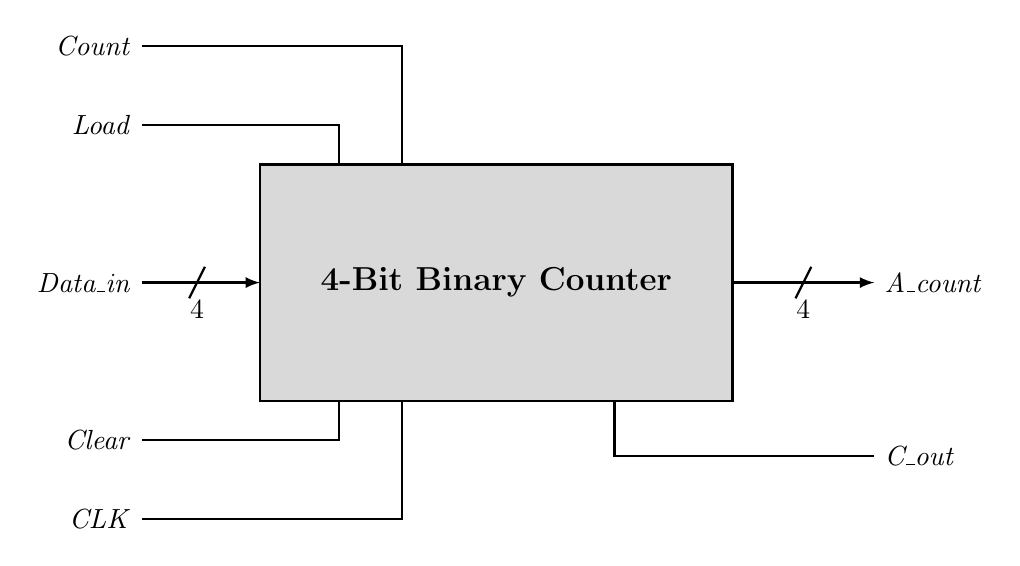
\begin{tikzpicture}[>=latex, thick]

    % ================= মূল ব্লক (Main Block) =================
    % ছবিটিতে ব্লকের ভেতরে একটি টেক্সচার/প্যাটার্ন দেখা যাচ্ছে, এখানে পরিষ্কার ও প্রফেশনাল লুকের জন্য হালকা ছাই রঙ (black!15) দেওয়া হয়েছে।
    \node[draw, rectangle, minimum width=6cm, minimum height=3cm, fill=black!15, font=\large\bfseries] (counter) at (0,0) {4-Bit Binary Counter};

    % ================= উপরের ইনপুটসমূহ (Top Inputs) =================
    % Count
    \draw (-4.5, 3.0) node[left] {\textit{Count}} -- (-1.2, 3.0) -- (-1.2, 1.5);
    % Load
    \draw (-4.5, 2) node[left] {\textit{Load}} -- (-2.0, 2) -- (-2.0, 1.5);

    % ================= বাম পাশের ইনপুট (Left Input) =================
    % Data_in (অ্যারো সহ)
    \draw[->] (-4.5, 0) node[left] {\textit{Data\_in}} -- (-3.0, 0);
    % Data_in এর বাস স্ল্যাশ (Bus Slash)
    \draw (-3.9, -0.2) -- (-3.7, 0.2);
    \node[below] at (-3.8, -0.1) {4};

    % ================= নিচের ইনপুটসমূহ (Bottom Inputs) =================
    % Clear
    \draw (-4.5, -2) node[left] {\textit{Clear}} -- (-2.0, -2) -- (-2.0, -1.5);
    % CLK
    \draw (-4.5, -3.0) node[left] {\textit{CLK}} -- (-1.2, -3.0) -- (-1.2, -1.5);

    % ================= ডান পাশের আউটপুট (Right Output) =================
    % A_count (অ্যারো সহ)
    \draw[->] (3.0, 0) -- (4.8, 0) node[right] {\textit{A\_count}};
    % A_count এর বাস স্ল্যাশ (Bus Slash)
    \draw (3.8, -0.2) -- (4.0, 0.2);
    \node[below] at (3.9, -0.1) {4};

    % ================= নিচের ডান পাশের আউটপুট (Bottom Right Output) =================
    % C_out
    \draw (1.5, -1.5) -- (1.5, -2.2) -- (4.8, -2.2) node[right] {\textit{C\_out}};

\end{tikzpicture}
\end{center}

\mk{12} \yr{CSE 205 | L-2/T-1 | 2015--16}


%% -- Q5: Sync counter 1→4→5→7→2→1 (uncertain year) --
\item Design a 3-bit binary up counter that counts $1 \to 2 \to 5 \to 7 \to 1\cdots$, where any invalid state goes to the immediate next valid state in the sequence. Use T Flip-Flops. Show the state diagram, state table, function equations, minimization (if necessary) and the circuit diagram.
\mk{15} \yr{CSE 205 | L-2/T-1 | 2014--15}


%% -- Q4: Modulo-6 counter using 4-bit binary counter (two ways) --
\item Design a 3-bit synchronous binary up counter that counts $1 \to 2 \to 4 \to 7 \to 1 \to \cdots$, where any invalid state goes to the immediate next state in the sequence. Use JK flip-flops. Show the state table, state diagram, function minimization (if necessary), and circuit diagram.
\mk{20} \yr{CSE 205 | L-2/T-1 | 2013--14}


%% -- Q3: 3-bit binary up counter 1-2-5-7, T FF, invalid states --
\item Design a synchronous counter with the following binary sequence: $0, 1, 3, 7, 6, 4$ and repeat. Use T flip-flops.
\mk{15} \yr{CSE 205 | L-2/T-1 | 2012--13}

%% -- Q2: 3-bit synchronous counter 1-2-4-7 with JK FF --
\end{enumerate}

%%──────────────────────────────────────────────────────────────────────
\subtopic{cG}{Synchronous Gray Code Counter}
\label{sub:s7-gray}

\begin{enumerate}

%% -- Q1: 3-bit Gray code counter using JK flip-flops --
\item Design a 3-bit synchronous Gray Code Counter using JK Flip-Flops. Show the state diagram, state table, function equations and the circuit diagram.
\mk{15} \yr{CSE 205 | L-2/T-1 | 2014--15}

\item Develop a synchronous 3-bit counter with a Gray code sequence using JK flip-flops.\\
\textit{(Hint: Gray code count sequence for a 2-bit counter is: $00, 01, 11, 10, 00, 01, \ldots$)}
\mk{18} \yr{CSE 205 | L-2/T-1 | 2011--12}


%% -- Q2: 3-bit synchronous gray code counter (JK FF) --
\end{enumerate}

%%──────────────────────────────────────────────────────────────────────
\subtopic{cG}{Switch-Tail Ring Counter}
\label{sub:s7-ring}

\begin{enumerate}

%% -- Q1: Four-stage switch-tail ring counter --
\item Design a 5-bit ring counter using a shift register and illustrate its operation using a timing diagram.
\mk{10} \yr{CSE 205 | L-2/T-1 | 2017--18}

\item Draw the logic diagram of a four-stage switch-tail ring counter.
\mk{5} \yr{CSE 205 | L-2/T-1 | 2011--12}


%% -- Q2: 5-bit ring counter with shift register; timing diagram (2017-18) --
\end{enumerate}

%%──────────────────────────────────────────────────────────────────────
\subtopic{cG}{Johnson Counter vs Ring Counter}
\label{sub:s7-johnson}

\begin{enumerate}

%% -- Q1: 4-bit Johnson counter, disadvantage, difference from ring --
\item Write a short note about a ring counter.
\mk{5} \yr{CSE 205 | L-2/T-1 | 2022--23}

\item Distinguish between a ring counter and a Johnson counter. Design a 5-bit ring counter and a 5-bit Johnson counter using shift registers and illustrate their operation using timing diagrams.
\mk{10} \yr{CSE 205 | L-2/T-1 | 2020--21}
\variant{2019--20}

%% -- Q4: Short note about a ring counter (2022-23) --
\item Design a 4-bit Johnson counter using a shift register and illustrate its operation using a timing diagram.
\mk{7} \yr{CSE 205 | L-2/T-1 | 2018--19}


%% -- Q3: Distinguish ring and Johnson counter; 5-bit versions with timing (2020-21) --
\item Design a 4-bit Johnson Counter. What is the disadvantage of a Johnson Counter? What is the difference between a Johnson Counter and a Ring Counter?
\mk{10} \yr{CSE 205 | L-2/T-1 | 2014--15}


%% -- Q2: 4-bit Johnson counter with shift register; timing diagram (2018-19) --
\end{enumerate}

%%──────────────────────────────────────────────────────────────────────
\subtopic{cG}{Counter Direction Analysis}
\label{sub:s7-direction}

\begin{enumerate}

%% -- Q1: Up/down direction from counter circuit with VDD --
\item A counter circuit has $V_{DD}$ assigned to Logic~1; the current values of LSB $Q_0$ and MSB $Q_1$ are 0 and~1 respectively. Find the direction (up or down) in which the circuit counts when the next clock pulse occurs. What would have to be altered to make the circuit count in the other direction?

\begin{center}
\begin{circuitikz}[scale=1, transform shape, thick]

  % --- First Flip-Flop (FF0) ---
  % Main Box
  \draw (2, 0) rectangle (4, 3);
  % Internal Pin Labels
  \node[right] at (2, 2.5) {J};
  \node[right] at (2, 1.5) {C};
  \node[right] at (2, 0.5) {K};
  \node[left] at (4, 2.5) {Q};
  \node[left] at (4, 0.5) {$\overline{\text{Q}}$};
  % Clock Triangle
  \draw (2, 1.7) -- (2.2, 1.5) -- (2, 1.3); 
  % Inversion Bubble for Q-bar
  \draw (4.1, 0.5) circle (0.1); 

  % --- Second Flip-Flop (FF1) ---
  % Main Box
  \draw (8, 0) rectangle (10, 3);
  % Internal Pin Labels
  \node[right] at (8, 2.5) {J};
  \node[right] at (8, 1.5) {C};
  \node[right] at (8, 0.5) {K};
  \node[left] at (10, 2.5) {Q};
  \node[left] at (10, 0.5) {$\overline{\text{Q}}$};
  % Clock Triangle
  \draw (8, 1.7) -- (8.2, 1.5) -- (8, 1.3); 
  % Inversion Bubble for Q-bar
  \draw (10.1, 0.5) circle (0.1); 

  % --- External Clock Routing ---
  \draw (0, 1.5) node[left]{Clock} -- (2, 1.5);
  \fill (0.5, 1.5) circle (2pt); % Connection dot for clock split
  % Clock line dropping down and routing to FF1
  \draw (0.5, 1.5) -- (0.5, -1) -- (6.5, -1) -- (6.5, 1.5) -- (8, 1.5);

  % --- VDD & FF0 Inputs Routing ---
  \draw (1.2, 2.5) -- (2, 2.5); % Wire to J
  \draw (1.2, 0.5) -- (2, 0.5); % Wire to K
  \fill (1.2, 2.5) circle (2pt); % Dot at J intersection
  
  % VDD Terminal Rail
  \draw (1.2, 2.5) -- (1.2, 3.5);
  \draw (0.9, 3.5) -- (1.5, 3.5) node[above, midway]{$\text{V}_{\text{DD}}$};
  
  % Vertical wire connecting J & K (with a jump over the clock line)
  \draw (1.2, 2.5) -- (1.2, 1.6);
  \draw (1.2, 1.6) arc (90:270:0.1); % Left-facing jump arc
  \draw (1.2, 1.4) -- (1.2, 0.5);

  % --- FF0 Outputs & FF1 Inputs Routing ---
  % FF0 Q0 Output
  \draw (4, 2.5) -- (5, 2.5) -- (5, 4.5) node[above]{$Q_0$};
  
  % FF0 Q-bar line routed to FF1 (with a jump over the vertical clock wire)
  \draw (4.2, 0.5) -- (6.4, 0.5);
  \draw (6.4, 0.5) arc (180:0:0.1); % Up-facing jump arc
  \draw (6.6, 0.5) -- (7.2, 0.5);
  
  % FF1 J-K input tie connections
  \fill (7.2, 0.5) circle (2pt); % Dot at K intersection
  \draw (7.2, 0.5) -- (8, 0.5);
  \draw (7.2, 2.5) -- (8, 2.5);
  
  % Vertical wire connecting J & K for FF1 (with jump over clock line)
  \draw (7.2, 0.5) -- (7.2, 1.4);
  \draw (7.2, 1.4) arc (-90:-270:0.1); % Left-facing jump arc
  \draw (7.2, 1.6) -- (7.2, 2.5);

  % --- FF1 Outputs Routing ---
  % FF1 Q1 Output
  \draw (10, 2.5) -- (11, 2.5) -- (11, 4.5) node[above]{$Q_1$};
  % FF1 Q-bar open stub
  \draw (10.2, 0.5) -- (11.5, 0.5);

\end{circuitikz}
\end{center}

\mk{7} \yr{CSE 205 | L-2/T-1 | 2015--16}

\end{enumerate}

%%──────────────────────────────────────────────────────────────────────
\subtopic{cG}{Clock Generator / Divider}
\label{sub:s7-clock}

\begin{enumerate}

%% -- Q1: 100 MHz -> 50 MHz and 25 MHz using D FF; timing diagram (2017-18) --
\item Given a 100\,MHz clock signal, derive a circuit using D flip-flops to generate 50\,MHz and 25\,MHz clock signals. Draw a timing diagram for all three clock signals.
\mk{10} \yr{CSE 205 | L-2/T-1 | 2017--18}

\end{enumerate}

%%──────────────────────────────────────────────────────────────────────
\subtopic{cG}{Universal Shift Register}
\label{sub:s7-universal}

\begin{enumerate}

%% -- Q1: 4-bit universal shift register using JK FF --
\item Design a 4-bit universal shift register using multiplexers and D flip-flops.
\mk{13} \yr{CSE 205 | L-2/T-1 | 2024--25}

%% -- Q6: Compare hardware efficiency of universal vs dedicated shift registers (2024-25) --
\item Compare the hardware efficiency and flexibility of universal shift registers with dedicated shift registers in complex digital systems.
\mk{7} \yr{CSE 205 | L-2/T-1 | 2024--25}

\item Use a 2-to-4 decoder, NAND gates and edge triggered D flip-flops to design a 4-bit shift register module that has the following functions:
\begin{center}
\begin{tabular}{|c|c|l|}
\hline
$S_1$ & $S_0$ & Mode \\
\hline
0 & 0 & Shift right (all 4 bits)\\
0 & 1 & Shift left (all 4 bits)\\
1 & 0 & Synchronous common clear \\
1 & 1 & Synchronous parallel load \\
\hline
\end{tabular}
\end{center}
\mk{10} \yr{CSE 205 | L-2/T-1 | 2021--22}

%% -- Q5: 4-bit universal shift register using MUX and D FF (2024-25) --
\item Draw the logic diagram of a 3-bit universal shift register with mode selection inputs $s_2$, $s_1$, $s_0$. The register operates with eight modes: (000) No change, (001) Invert all bits, (010) Set all bits to 0, (011) Set all bits to 1, (100) Parallel load, (101) Shift left, (110) Shift right, (111) No change.
\mk{15} \yr{CSE 205 | L-2/T-1 | 2016--17}

%% -- Q4: 4-bit shift register module with decoder and D FF; 4 modes (2021-22) --
\item Draw the logic diagram of a two-bit register with two D flip-flops and two $4\times1$ multiplexers with mode selection inputs $s_1$ and $s_0$. The register operates with four modes: (00) No change, (01) Complement the two outputs, (10) Clear register to 0 (synchronous), (11) Load parallel data.
\mk{12} \yr{CSE 205 | L-2/T-1 | 2015--16}


%% -- Q3: 3-bit universal shift register with 8 modes (s2,s1,s0) (2016-17) --
\item Draw the circuit diagram of a 4-bit universal shift register using JK flip-flops.
\mk{12} \yr{CSE 205 | L-2/T-1 | 2012--13}


%% -- Q2: 2-bit register with D FF + 4x1 MUX, mode control s1,s0 --
\end{enumerate}

%%──────────────────────────────────────────────────────────────────────
\subtopic{cG}{Serial Adder \& Serial Subtractor}
\label{sub:s7-serial}

\begin{enumerate}

%% -- Q1: Serial adder with clock-by-clock trace (0101 + 0011) --
\item A 4-bit shift register is used for serial data transmission.
\begin{enumerate}
  \item Analyze the timing relationship between input data, clock and output.
  \item Explain how errors may propagate in serial communication using shift registers.
\end{enumerate}
\mk{16} \yr{CSE 205 | L-2/T-1 | 2024--25}

\item Design a sequential circuit to copy the content of shift register $A$ to shift register $B$. Use a block diagram to represent the shift register in the diagram.
\mk{12} \yr{CSE 205 | L-2/T-1 | 2022--23}

%% -- Q7: 4-bit shift register for serial data transmission; timing and error propagation (2024-25) --
\item Design a serial subtractor that will perform the operation $A - B$, where $A = a_{n-1}\ldots a_1 a_0$ and $B = b_{n-1}\ldots b_1 b_0$. The operands are applied to the serial subtractor sequentially, beginning with bits $a_0$ and $b_0$. Use JK flip-flops in your design.
\mk{10} \yr{CSE 205 | L-2/T-1 | 2021--22}

%% -- Q6: Sequential circuit to copy shift register A to B (2022-23) --
\item Design a serial adder that computes the sum of two 4-bit binary numbers $A$ and $B$ stored in individual shift registers. The result of the addition is stored in the shift register representing $A$.
\mk{10} \yr{CSE 205 | L-2/T-1 | 2017--18}

%% -- Q5: Serial subtractor A-B with JK FF (2021-22) --
\item Design a serial adder that computes the sum of two 4-bit binary numbers $A$ and $B$ stored in individual shift registers. The result of the addition is stored in the shift register representing $A$. Use the sequential logic design procedure.
\mk{10} \yr{CSE 205 | L-2/T-1 | 2016--17}

%% -- Q4: Serial adder (repeat 2017-18) --
\item Design a serial subtractor that subtracts the content of register $B$ from the content of register $A$, where the contents of $A$ and $B$ are stored in individual shift registers. The result of the subtraction is stored in the shift register representing $A$. (Both $A$ and $B$ are 4-bit binary numbers.)
\mk{10} \yr{CSE 205 | L-2/T-1 | 2013--14}


%% -- Q3: Serial adder for two 4-bit numbers (2016-17) --
\item Draw the logic diagram of a serial adder. Show the values of inputs and outputs of all components (e.g., flip-flop, register) used in the design after every clock pulse while adding the following two numbers: $0101$ and $0011$.
\mk{6+6} \yr{CSE 205 | L-2/T-1 | 2011--12, 2012--13}

%% -- Q2: Serial subtractor (B from A in shift registers) --
\end{enumerate}


%% ══════════════════════════════════════════════════════════════════════
%%  SECTION 8: MEMORY & PROGRAMMABLE LOGIC
%% ══════════════════════════════════════════════════════════════════════
\secdivider{Memory \& Programmable Logic}{RAM, ROM, Address Multiplexing, PLA Design}{cH}{cyan!30!black}

\markboth{S8: Memory \& Programmable Logic}{S8: Memory \& Programmable Logic}
\label{sec:S8}
\titleformat{\section}{\large\bfseries\color{cH}}{}{0em}{}[\titlerule]
\section*{S8 \quad Memory \& Programmable Logic}
\addcontentsline{toc}{section}{S8: Memory \& Programmable Logic}

%%──────────────────────────────────────────────────────────────────────
\subtopic{cH}{ROM Design \& Expansion}
\label{sub:s8-rom}

\begin{enumerate}

%% -- Q1: 128x4 ROM using 32x4 ROMs --
\item You have several $32 \times 4$ ROMs in the laboratory. Each ROM can be enabled/disabled using a 1/0 signal respectively. How would you implement a $128 \times 4$ ROM using the available ROMs? You may use any additional circuitry if needed.
\mk{10} \yr{CSE 205 | L-2/T-1 | 2013--14}

\end{enumerate}

%%──────────────────────────────────────────────────────────────────────
\subtopic{cH}{PLA Design}
\label{sub:s8-pla}

\begin{enumerate}

%% -- Q1: PLA for three Boolean functions --
\item Design a PLA to implement the following functions with the minimization of the number of product terms:
\begin{align*}
  F_1(x, y, z) &= \Sigma\,(1,3,5,6),\quad & F_2(x, y, z) &= \Sigma\,(0,1,6,7) \\
  F_3(x, y, z) &= \Sigma\,(3,5),\quad & F_4(x, y, z) &= \Sigma\,(1,2,4,5,7)
\end{align*}
\mk{15} \yr{CSE 205 | L-2/T-1 | 2024--25}

\item Tabulate the PLA programming table for the two Boolean functions listed below. Minimize the numbers of product terms:
\begin{align*}
  F_1(A, B, C) &= \Sigma\,(0, 1, 2, 4) \\
  F_2(A, B, C) &= \Sigma\,(0, 5, 6, 7)
\end{align*}
\mk{15} \yr{CSE 205 | L-2/T-1 | 2022--23}

%% -- Q10: PLA for four functions F1-F4; minimize product terms (2024-25) --
\item A combinational circuit is defined by the following two functions:
\begin{align*}
  F_1(A, B, C) &= \Sigma\,(3, 5, 6, 7) \\
  F_2(A, B, C) &= \Sigma\,(0, 2, 4, 7)
\end{align*}
The circuit needs to be implemented with a PLA having three inputs, four product terms, and two outputs. Show the PLA programming table.
\mk{15} \yr{CSE 205 | L-2/T-1 | 2021--22}

%% -- Q9: PLA programming table for two functions; minimize product terms (2022-23) --
\item Design a digital security lock using PLA which takes BCD as input and opens after converting the input to Excess-3 code. Use the minimum number of product terms. (Show the fuse map.)
\mk{15} \yr{CSE 205 | L-2/T-1 | 2020--21}


%% -- Q7: PLA design for two 3-variable functions (2019-20) --
\item Design a circuit for the following functions using a Programmable Logic Array (PLA):
\begin{align*}
  A(x,y,z) &= \Sigma\,(0,1,2,5,7) \\
  B(x,y,z) &= \Sigma\,(0,1,3,6,7)
\end{align*}
\mk{10} \yr{CSE 205 | L-2/T-1 | 2019--20}

%% -- Q8: PLA for two functions F1 and F2; 3 inputs, 4 product terms, 2 outputs (2021-22) --
\item Design a security lock using PLA which will be opened using the following combinations:
\begin{align*}
  A(x,y,z) &= \Sigma\,(1,3,5,6),\quad B(x,y,z) = \Sigma\,(0,1,6,7) \\
  C(x,y,z) &= \Sigma\,(3,5),\quad D(x,y,z) = \Sigma\,(1,3,4,5,7)
\end{align*}
\mk{12} \yr{CSE 205 | L-2/T-1 | 2018--19}

%% -- Q6: Digital security lock using PLA with BCD-to-Excess-3 conversion (2020-21) --
\item For a given Programmable Logic Array (PLA), find the function expressions for $F_1$ and $F_2$ and show the PLA programming table.

\begin{center}
  \begin{circuitikz}[thick, scale=0.9, transform shape]
  
  % Vertical lines for inputs (C, C', B, B', A, A' from left to right based on the diagram)
  \foreach \x/\label in {2/C, 2.5/C', 3/B, 3.5/B', 4/A, 4.5/A'} {
      \draw (\x, 0.5) -- (\x, 9);
      \node[below] at (\x, 0.5) {$\label$};
  }

  % Define a custom macro to draw the input buffer/splitter
  % \plasplitter{y_position}{Name}{x_normal}{x_inverted}
  \newcommand{\plasplitter}[4]{
    \draw (0.2, #1) node[left]{#2} -- (0.8, #1);
    \draw (0.8, #1+0.3) -- (0.8, #1-0.3) -- (1.6, #1) -- cycle; % Triangle
    \draw (1.6, #1+0.15) circle (0.08); % Bubble for inverted output
    \draw (1.6+0.08, #1+0.15) -- (#4, #1+0.15); % Line to inverted vertical
    \fill (#4, #1+0.15) circle (2pt); % Connection dot
    \draw (1.6, #1-0.15) -- (#3, #1-0.15); % Line to normal vertical
    \fill (#3, #1-0.15) circle (2pt); % Connection dot
  }
  
  % Draw the 3 input splitters at the top left
  \plasplitter{8.5}{A}{4}{4.5}
  \plasplitter{7.5}{B}{3}{3.5}
  \plasplitter{6.5}{C}{2}{2.5}

  % AND plane (4 AND gates)
  \foreach \y/\id in {5.5/1, 4/2, 2.5/3, 1/4} {
      \node[and port, no input leads] (AND\id) at (6, \y) {};
      \node at (AND\id.center) {\id};
      \draw (1.8, \y) -- (4.9,\y); % Input line to AND gate
      \draw (AND\id.out) -- (10, \y);  % Output line extending right
  }
  
  % Programmable connection dots in the AND plane
  % AND1: C, B, A
 
  \node[or port, rotate=-90, no input leads] (OR1) at (7.5, -1) {};
  \node[or port, rotate=-90, no input leads] (OR2) at (9, -1) {};
  % OR plane (2 OR gates facing downwards)
  % Vertical lines for OR inputs
  \draw (7.5,-.1) -- ++(0,6);
  \draw (9,-.1) -- ++(0,6);


  
  

  % XOR plane (2 XOR gates)
  \node[xor port] (XOR1) at (13, -2) {}; % Top XOR (F1)
  \node[xor port] (XOR2) at (13, -3.5) {}; % Bottom XOR (F2)
  
  % Connect OR outputs to the top inputs of XOR gates
  % Right OR gate connects to F1 (top XOR)
  \draw (OR2.out) |- (XOR1.in 1);
  % Left OR gate connects to F2 (bottom XOR)
  \draw (OR1.out) |- (XOR2.in 1);

  % Programmable polarity lines (0 and 1)
  \draw (10, -0.5) -- (13, -0.5) node[right]{0};
  \draw (10, -1.0) -- (13, -1.0) node[right]{1};
  
  % Connect bottom inputs of XOR gates to polarity lines
  % XOR1 (F1) connects to '1'
  \draw (XOR1.in 2) -- (11, -2.5) -- (11, -0.3);
  
  % XOR2 (F2) connects to '0'
  \draw (XOR2.in 2) -- (10.5, -3.78) -- (10.5, -0.3);

  % Final Outputs
  \node[right] at (XOR1.out) {$F_1$};
  \node[right] at (XOR2.out) {$F_2$};

\end{circuitikz}
\end{center}

\mk{13} \yr{CSE 205 | L-2/T-1 | 2015--16}


%% -- Q5: Security lock using PLA (2018-19) --
\item Write the difference between ROM and PLA. A combinational circuit is defined by the following functions:
\begin{align*}
  F_1(A,B,C) &= \Sigma\,(0,1,2,4) \\
  F_2(A,B,C) &= \Sigma\,(0,5,6,7)
\end{align*}
Implement the circuit with a PLA having three inputs, four product terms and two outputs.
\mk{5+10} \yr{CSE 205 | L-2/T-1 | 2014--15}


%% -- Q4: PLA analysis -- find F1, F2, programming table --
\item Derive the PLA program table for a combinational circuit that squares a 3-bit binary number. Minimize the number of product terms.
\mk{25} \yr{CSE 205 | L-2/T-1 | 2013--14}


%% -- Q3: ROM vs PLA; PLA for F1,F2 --
\item Implement the following three Boolean functions with a PLA:
\begin{align*}
  F_1 &= \Sigma\,(0,1,2,4) \\
  F_2 &= \Sigma\,(0,5,6,7) \\
  F_3 &= \Sigma\,(0,3,5,7)
\end{align*}
\mk{15} \yr{CSE 205 | L-2/T-1 | 2011--12}

%% -- Q2: PLA program table for 3-bit squarer --
\end{enumerate}

%%──────────────────────────────────────────────────────────────────────
\subtopic{cH}{RAM Design}
\label{sub:s8-ram}

\begin{enumerate}

%% -- Q1: Two-dimensional decoding for 1K word memory; cost optimization (2024-25) --
\item If you use two dimensional decoding for addressing a 1K word memory, can you optimize the cost? Justify your answer.
\mk{8} \yr{CSE 205 | L-2/T-1 | 2024--25}

\end{enumerate}

%% -- S6: Synchronous sequential traffic light and divide-by-three (2023-24) --

%%──────────────────────────────────────────────────────────────────────
\subtopic{cF}{Synchronous Sequential Circuit Design}
\label{sub:s6-sync-design}

\begin{enumerate}

%% -- Q1: Traffic light controller NS-EW; WALK button; D flip-flops (2023-24) --
\item Design an automatic vending machine, when the candy bars inside the machine cost 3\,Tk and the machine accepts 1\,Tk and 2\,Tk only. The system accepts the bills sequentially. The circuit produces a level output that delivers the candy whenever the amount received by the machine is 3\,Tk or more. The excess amount is kept deposited for the next candy. Design a synchronous sequential circuit for the vending machine using S-R flip-flops. Provide the circuit diagram as well.
\mk{25} \yr{CSE 205 | L-2/T-1 | 2024--25}

\item Design a simplified traffic-light controller that switches traffic lights on a crossing where a north-south (NS) street intersects an east-west (EW) street. The input to the controller is the WALK button pushed by pedestrians who want to cross the street. The outputs are two signals NS and EW that control the traffic lights in NS and EW directions. When NS or EW are 0, the red light is on and when they are 1, the green light is on. When there are no pedestrians, $\text{NS}=0$ and $\text{EW}=1$ for 1 minute, followed by $\text{NS}=1$ and $\text{EW}=0$ for 1 minute and so on. When a WALK button is pushed, NS and EW both come 1 for a minute when the present minute expires. After that the NS and EW signals continue alternating. For the traffic-light controller:
	(i) Develop a state diagram and state/output table.
	(ii) Find the transition and excitation tables using S-R flipflops.
	(iii) Draw a circuit diagram.
  \mk{23} \yr{CSE 205 | L-2/T-1 | 2023--24}

%% -- Q2: Divide-by-three counter; counts 1s from input stream; D FF (2023-24) --
\item Design a divide-by-three counter which counts the number of `1's from an input sequence of binary stream. This counter outputs one 1 for every three 1's seen as input (not necessarily in succession). After outputting a 1, it starts counting all over again. Design the counter using D flip-flops.
\mk{12} \yr{CSE 205 | L-2/T-1 | 2023--24}

%% -- Q3: Vending machine synchronous 3Tk; level output; SR FF (2024-25) --
\end{enumerate}


\end{document}